\documentclass[a4paper,landscape,10pt]{article}
\usepackage[margin=10mm, top=18mm, bottom=12mm, headheight=14pt, headsep=4mm, footskip=6mm]{geometry}
\usepackage[T1]{fontenc}
\usepackage{lmodern}
\usepackage{helvet}
\renewcommand{\familydefault}{\sfdefault}
\usepackage{tikz}
\usetikzlibrary{arrows.meta}
\usepackage{xcolor}
\usepackage{booktabs}
\setlength{\parindent}{0pt}
\definecolor{ft0}{HTML}{CFE4F2}
\definecolor{ft1}{HTML}{FBE2B4}
\definecolor{ft2}{HTML}{D4E9CC}
\definecolor{ft3}{HTML}{E5D3EA}
\definecolor{ft4}{HTML}{F5CACA}
\usepackage{fancyhdr}
\usepackage[hidelinks, bookmarksnumbered, bookmarksopen, bookmarksopenlevel=1]{hyperref}
\setcounter{tocdepth}{2}
\setcounter{secnumdepth}{1}
\renewcommand{\sectionmark}[1]{\markboth{#1}{}}
\pagestyle{fancy}
\fancyhf{}
\renewcommand{\headrulewidth}{0.3pt}
\fancyhead[L]{\small Bilderwand -- layout candidates}
\fancyhead[R]{\small\nouppercase{\leftmark}}
\fancyfoot[C]{\small\thepage}
\begin{document}

\thispagestyle{empty}
\vspace*{18mm}
\begin{center}
{\Huge\bfseries Bilderwand -- layout candidates}\\[10pt]
{\LARGE 9 search paradigms, 144 layouts}\\[8pt]
{\large 25 October 2026}
\end{center}
\vspace{14mm}
\begin{minipage}[t]{0.58\textwidth}\vspace{0pt}
{\bfseries What this document is}\\[4pt]
The 28 picture frames listed on the right (measured outer dimensions, orientation as listed) are
to be hung as one collage of about 180 $\times$ 120 cm
($\pm$ 10 cm) with gaps as uniform as possible and, ideally, a sharp rectangular
outer border. Not all frames have to be used.

\vspace{6pt}
The same search was run with 9 different settings (``paradigms'': free-gap, per-run-gap, proportional, gap-3, linear-cost, free-gap-s1, large-apart, entropy, large-entropy).
Section~1 explains what distinguishes them and compares their best layouts, section~2 ranks all
144 distinct layouts of this document together, section~3 covers the sub-analysis with large-frame constraints and the entropy reward, and the remaining sections show every paradigm's
16 best layouts, one per page at scale 1:10, with frame labels, red annotations for gaps that
deviate from the nominal gap, and a coordinate table for hanging.

\vspace{6pt}
{\bfseries Reading the numbers}\\[4pt]
\emph{Nominal gap}: the spacing the layout is built on. \emph{Max.\ / mean deviation}: largest and
average difference between an actual gap and the nominal gap, in cm.
\emph{Notches}: total length of the outer border that is not covered by a frame or a regular gap.
\emph{Corners}: how many of the four corners of the bounding rectangle are filled by a frame.
\emph{Score} $=$ max.\ deviation $+ 0.5\cdot$ mean deviation $+ 0.15\cdot$ notch length $+ 2$ per
missing corner (lower is better). Layouts are ranked by score rounded to whole cm, then by number of frames
(more is better), then by exact score, then by distance from the target size.
\emph{Entropy}: irregularity of the constellation in $[0, 1]$ (mix of formats, different neighbours, staggered
edges, few through-lines; see the sub-analysis section). \emph{Large frames}: the 52.5 $\times$ 42.5 and
42.5 $\times$ 52.5 frames; a layout page says how many are used, whether two of them touch and how far apart the
closest two are.
\end{minipage}\hfill
\begin{minipage}[t]{0.36\textwidth}\vspace{0pt}
{\bfseries Inventory}\\[4pt]
\begin{tabular}{@{}c l l r@{}}
\toprule
 & outer w $\times$ h (cm) &  & have \\
\midrule
\tikz[baseline=-0.6ex]\fill[ft0,draw=black!60] (0,0) rectangle (1.2ex,1.2ex); & 20.5$\times$15.5 & L & 9 \\
\tikz[baseline=-0.6ex]\fill[ft0,draw=black!60] (0,0) rectangle (1.2ex,1.2ex); & 15.5$\times$20.5 & P & 2 \\
\tikz[baseline=-0.6ex]\fill[ft3,draw=black!60] (0,0) rectangle (1.2ex,1.2ex); & 32.5$\times$42.5 & P & 2 \\
\tikz[baseline=-0.6ex]\fill[ft3,draw=black!60] (0,0) rectangle (1.2ex,1.2ex); & 42.5$\times$32.5 & L & 1 \\
\tikz[baseline=-0.6ex]\fill[ft1,draw=black!60] (0,0) rectangle (1.2ex,1.2ex); & 32.5$\times$23.5 & L & 5 \\
\tikz[baseline=-0.6ex]\fill[ft1,draw=black!60] (0,0) rectangle (1.2ex,1.2ex); & 23.5$\times$32.5 & P & 1 \\
\tikz[baseline=-0.6ex]\fill[ft2,draw=black!60] (0,0) rectangle (1.2ex,1.2ex); & 25.5$\times$25.5 &  & 5 \\
\tikz[baseline=-0.6ex]\fill[ft4,draw=black!60] (0,0) rectangle (1.2ex,1.2ex); & 42.5$\times$52.5 & P & 1 \\
\tikz[baseline=-0.6ex]\fill[ft4,draw=black!60] (0,0) rectangle (1.2ex,1.2ex); & 52.5$\times$42.5 & L & 2 \\
\bottomrule
\end{tabular}
\end{minipage}
\clearpage
\tableofcontents
\clearpage

\section{Search paradigms}\label{sec:paradigms}
All paradigms share the same model and search. A layout is a \emph{slicing tree} over a subset of the
frames: frames are recursively placed side by side or on top of each other with a nominal gap. Where two
siblings differ in height (or width) the smaller one has slack, which is absorbed by widening the gaps inside
it; if it has no inner gaps the slack becomes dead space, which counts as a notch when it touches the outer
border. Simulated annealing over the tree, the subset of frames used and (unless fixed) the nominal gap
minimises a cost made of gap deviations, border notches, the distance from the target size and a small bonus
per frame used. Every paradigm ran 256 independent annealing runs, 20 min wall-clock budget on all cores;
its candidate states were then placed, measured exactly, de-duplicated (mirror images count as equal) and
ranked by the score described on the title page.

\vspace{8pt}
\begin{tabular}{@{}l p{0.50\textwidth} p{0.30\textwidth}@{}}
\toprule
paradigm & what differs & parameters that differ from the baseline \\
\midrule
\hyperref[sec:free-gap]{\bfseries free-gap} & Baseline. The nominal gap is an annealing variable between 1.5 and 6 cm (steps of 0.5 cm). Where a strip of frames is shorter than its neighbour, the slack is spread evenly over the gaps inside that strip. Gap deviations and border notches are penalised with a Huber shape: quadratic up to 2 cm, linear beyond, so a few large deviations are not punished out of proportion. & {\small baseline} \\
\addlinespace[4pt]
\hyperref[sec:per-run-gap]{\bfseries per-run-gap} & Every annealing run keeps one fixed nominal gap from the grid 1.5, 2, \dots, 6 cm (the runs are spread over the grid) instead of changing the gap during the search. Each run explores its gap value more thoroughly, which gives a more diverse set of results across gap values. & {\small gap\_mode = per-run} \\
\addlinespace[4pt]
\hyperref[sec:proportional]{\bfseries proportional} & Unavoidable slack is distributed in proportion to the size of the neighbouring frames: the weight of a gap is the mean extent of the two frames (or groups) it separates, so gaps next to big frames widen more than gaps between small ones. The deviations are therefore systematic (bigger frame, bigger gap) rather than equal. & {\small slack\_rule = proportional} \\
\addlinespace[4pt]
\hyperref[sec:gap-3]{\bfseries gap-3} & The nominal gap is fixed at 3 cm; the search only changes the arrangement and the subset of frames. Actual gaps still deviate from 3 cm wherever slack has to be absorbed. & {\small gap = 3} \\
\addlinespace[4pt]
\hyperref[sec:linear-cost]{\bfseries linear-cost} & Gap deviations and notches are penalised linearly instead of with the Huber shape. The cost landscape is smoother and small deviations count relatively more, which favours layouts whose deviations are spread thinly instead of concentrated in one gap. & {\small cost\_shape = linear} \\
\addlinespace[4pt]
\hyperref[sec:free-gap-s1]{\bfseries free-gap-s1} & Identical to the baseline but with another random seed. Comparing it with the baseline shows how reproducible the results of a 20 minute search are. & {\small seed = 1} \\
\addlinespace[4pt]
\hyperref[sec:large-apart]{\bfseries large-apart} & Sub-analysis. Like the baseline, but the layout must contain 2 to 3 large frames (outer area of at least 2000 cm$^2$, i.e.\ the 52.5 $\times$ 42.5 and 42.5 $\times$ 52.5 frames) and they are kept apart: two large frames that are direct neighbours are penalised in proportion to the edge they share (barely touching costs little), and the closest pair of large frames is pulled towards a centre distance of at least 70 cm. & {\small large\_area = 2000, large\_count = 2-3, large\_apart = True, large\_min\_dist = 70, entropy = 0} \\
\addlinespace[4pt]
\hyperref[sec:entropy]{\bfseries entropy} & Sub-analysis. Like the baseline, but the cost also rewards the irregularity (``entropy'') of the constellation: a mix of many formats, different formats next to each other, frame edges that do not line up, and few straight gap lines running across the whole collage. & {\small large\_apart = False, large\_min\_dist = 70, entropy = 40} \\
\addlinespace[4pt]
\hyperref[sec:large-entropy]{\bfseries large-entropy} & Sub-analysis. Both of the above: 2 to 3 large frames kept apart from each other, and the irregularity reward. & {\small large\_area = 2000, large\_count = 2-3, large\_apart = True, large\_min\_dist = 70, entropy = 40} \\
\addlinespace[4pt]
\bottomrule
\end{tabular}

\vspace{12pt}
{\bfseries Best-ranked layout of each paradigm} (all measurements in cm)\\[4pt]
\begin{tabular}{@{}l r l r r r r l c r r@{}}
\toprule
paradigm & layout & size & frames & nominal gap & mean dev & max dev & notches & corners & entropy & score \\
\midrule
\hyperref[sec:free-gap]{free-gap} & \hyperref[lay:free-gap:1]{1} & 181.5 $\times$ 113.5 & 20 & 1.5 & 0.59 & 1.0 & none & 4/4 & 0.71 & 1.29 \\
\hyperref[sec:per-run-gap]{per-run-gap} & \hyperref[lay:per-run-gap:1]{1} & 188.0 $\times$ 113.5 & 24 & 2 & 0.62 & 3.0 & none & 4/4 & 0.76 & 3.31 \\
\hyperref[sec:proportional]{proportional} & \hyperref[lay:proportional:1]{1} & 185.5 $\times$ 116.5 & 23 & 2.5 & 0.51 & 2.0 & none & 4/4 & 0.77 & 2.25 \\
\hyperref[sec:gap-3]{gap-3} & \hyperref[lay:gap-3:1]{1} & 179.0 $\times$ 126.5 & 24 & 3 & 0.44 & 2.2 & none & 4/4 & 0.64 & 2.47 \\
\hyperref[sec:linear-cost]{linear-cost} & \hyperref[lay:linear-cost:1]{1} & 172.5 $\times$ 115.5 & 24 & 2.5 & 0.30 & 2.0 & none & 4/4 & 0.71 & 2.15 \\
\hyperref[sec:free-gap-s1]{free-gap-s1} & \hyperref[lay:free-gap-s1:1]{1} & 170.0 $\times$ 114.5 & 24 & 2 & 0.33 & 1.8 & 4 cm & 4/4 & 0.66 & 2.44 \\
\hyperref[sec:large-apart]{large-apart} & \hyperref[lay:large-apart:1]{1} & 182.0 $\times$ 129.0 & 25 & 4 & 0.60 & 3.0 & none & 4/4 & 0.65 & 3.30 \\
\hyperref[sec:entropy]{entropy} & \hyperref[lay:entropy:1]{1} & 172.5 $\times$ 116.5 & 24 & 2.5 & 0.43 & 2.0 & none & 4/4 & 0.72 & 2.21 \\
\hyperref[sec:large-entropy]{large-entropy} & \hyperref[lay:large-entropy:1]{1} & 182.0 $\times$ 129.0 & 24 & 4 & 0.56 & 1.8 & none & 4/4 & 0.65 & 2.03 \\
\bottomrule
\end{tabular}
\clearpage
{\large\bfseries Best-ranked layout of each paradigm at a glance} {\small (scale 1:25; details on the linked pages)}\\[10pt]
\begin{minipage}[t]{0.32\textwidth}\centering\vspace{0pt}
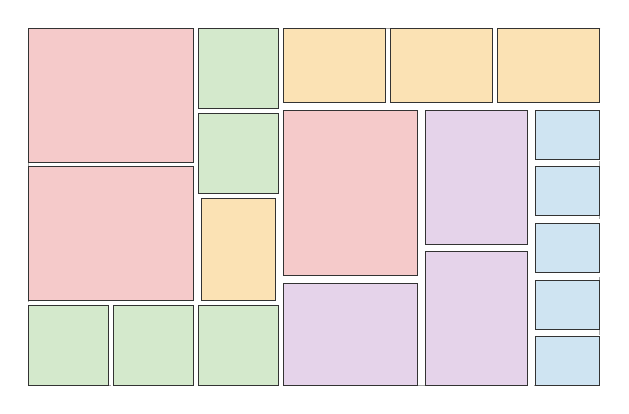
\begin{tikzpicture}[x=0.4mm, y=-0.4mm]
\draw[gray!70, dashed, line width=0.4pt] (0,0) rectangle (181.50,113.50);
\filldraw[fill=ft4, draw=black!80, line width=0.3pt] (0.00,0.00) rectangle (52.50,42.50);
\filldraw[fill=ft2, draw=black!80, line width=0.3pt] (54.00,0.00) rectangle (79.50,25.50);
\filldraw[fill=ft1, draw=black!80, line width=0.3pt] (81.00,0.00) rectangle (113.50,23.50);
\filldraw[fill=ft1, draw=black!80, line width=0.3pt] (115.00,0.00) rectangle (147.50,23.50);
\filldraw[fill=ft1, draw=black!80, line width=0.3pt] (149.00,0.00) rectangle (181.50,23.50);
\filldraw[fill=ft4, draw=black!80, line width=0.3pt] (81.00,26.00) rectangle (123.50,78.50);
\filldraw[fill=ft3, draw=black!80, line width=0.3pt] (126.00,26.00) rectangle (158.50,68.50);
\filldraw[fill=ft0, draw=black!80, line width=0.3pt] (161.00,26.00) rectangle (181.50,41.50);
\filldraw[fill=ft2, draw=black!80, line width=0.3pt] (54.00,27.00) rectangle (79.50,52.50);
\filldraw[fill=ft4, draw=black!80, line width=0.3pt] (0.00,44.00) rectangle (52.50,86.50);
\filldraw[fill=ft0, draw=black!80, line width=0.3pt] (161.00,44.00) rectangle (181.50,59.50);
\filldraw[fill=ft1, draw=black!80, line width=0.3pt] (55.00,54.00) rectangle (78.50,86.50);
\filldraw[fill=ft0, draw=black!80, line width=0.3pt] (161.00,62.00) rectangle (181.50,77.50);
\filldraw[fill=ft3, draw=black!80, line width=0.3pt] (126.00,71.00) rectangle (158.50,113.50);
\filldraw[fill=ft0, draw=black!80, line width=0.3pt] (161.00,80.00) rectangle (181.50,95.50);
\filldraw[fill=ft3, draw=black!80, line width=0.3pt] (81.00,81.00) rectangle (123.50,113.50);
\filldraw[fill=ft2, draw=black!80, line width=0.3pt] (0.00,88.00) rectangle (25.50,113.50);
\filldraw[fill=ft2, draw=black!80, line width=0.3pt] (27.00,88.00) rectangle (52.50,113.50);
\filldraw[fill=ft2, draw=black!80, line width=0.3pt] (54.00,88.00) rectangle (79.50,113.50);
\filldraw[fill=ft0, draw=black!80, line width=0.3pt] (161.00,98.00) rectangle (181.50,113.50);
\end{tikzpicture}\\[2pt]
{\small\bfseries free-gap} -- \hyperref[lay:free-gap:1]{layout 1}\\
{\scriptsize 181.5 $\times$ 113.5 cm, 20 frames, gap 1.5 cm,
max.\ dev.\ 1.0 cm, notches none, entropy 0.71}
\end{minipage}\hfill
\begin{minipage}[t]{0.32\textwidth}\centering\vspace{0pt}
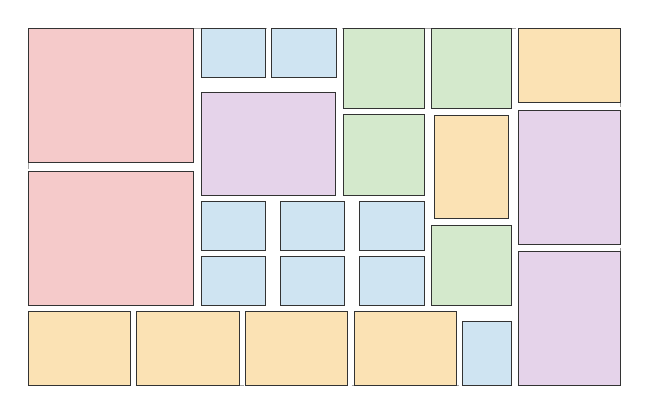
\begin{tikzpicture}[x=0.4mm, y=-0.4mm]
\draw[gray!70, dashed, line width=0.4pt] (0,0) rectangle (188.00,113.50);
\filldraw[fill=ft4, draw=black!80, line width=0.3pt] (0.00,0.00) rectangle (52.50,42.50);
\filldraw[fill=ft0, draw=black!80, line width=0.3pt] (54.83,0.00) rectangle (75.33,15.50);
\filldraw[fill=ft0, draw=black!80, line width=0.3pt] (77.33,0.00) rectangle (97.83,15.50);
\filldraw[fill=ft2, draw=black!80, line width=0.3pt] (100.17,0.00) rectangle (125.67,25.50);
\filldraw[fill=ft2, draw=black!80, line width=0.3pt] (128.00,0.00) rectangle (153.50,25.50);
\filldraw[fill=ft1, draw=black!80, line width=0.3pt] (155.50,0.00) rectangle (188.00,23.50);
\filldraw[fill=ft3, draw=black!80, line width=0.3pt] (55.08,20.50) rectangle (97.58,53.00);
\filldraw[fill=ft3, draw=black!80, line width=0.3pt] (155.50,26.00) rectangle (188.00,68.50);
\filldraw[fill=ft2, draw=black!80, line width=0.3pt] (100.17,27.50) rectangle (125.67,53.00);
\filldraw[fill=ft1, draw=black!80, line width=0.3pt] (129.00,27.75) rectangle (152.50,60.25);
\filldraw[fill=ft4, draw=black!80, line width=0.3pt] (0.00,45.50) rectangle (52.50,88.00);
\filldraw[fill=ft0, draw=black!80, line width=0.3pt] (54.83,55.00) rectangle (75.33,70.50);
\filldraw[fill=ft0, draw=black!80, line width=0.3pt] (80.00,55.00) rectangle (100.50,70.50);
\filldraw[fill=ft0, draw=black!80, line width=0.3pt] (105.17,55.00) rectangle (125.67,70.50);
\filldraw[fill=ft2, draw=black!80, line width=0.3pt] (128.00,62.50) rectangle (153.50,88.00);
\filldraw[fill=ft3, draw=black!80, line width=0.3pt] (155.50,71.00) rectangle (188.00,113.50);
\filldraw[fill=ft0, draw=black!80, line width=0.3pt] (54.83,72.50) rectangle (75.33,88.00);
\filldraw[fill=ft0, draw=black!80, line width=0.3pt] (80.00,72.50) rectangle (100.50,88.00);
\filldraw[fill=ft0, draw=black!80, line width=0.3pt] (105.17,72.50) rectangle (125.67,88.00);
\filldraw[fill=ft1, draw=black!80, line width=0.3pt] (0.00,90.00) rectangle (32.50,113.50);
\filldraw[fill=ft1, draw=black!80, line width=0.3pt] (34.50,90.00) rectangle (67.00,113.50);
\filldraw[fill=ft1, draw=black!80, line width=0.3pt] (69.00,90.00) rectangle (101.50,113.50);
\filldraw[fill=ft1, draw=black!80, line width=0.3pt] (103.50,90.00) rectangle (136.00,113.50);
\filldraw[fill=ft0, draw=black!80, line width=0.3pt] (138.00,93.00) rectangle (153.50,113.50);
\end{tikzpicture}\\[2pt]
{\small\bfseries per-run-gap} -- \hyperref[lay:per-run-gap:1]{layout 1}\\
{\scriptsize 188.0 $\times$ 113.5 cm, 24 frames, gap 2 cm,
max.\ dev.\ 3.0 cm, notches none, entropy 0.76}
\end{minipage}\hfill
\begin{minipage}[t]{0.32\textwidth}\centering\vspace{0pt}
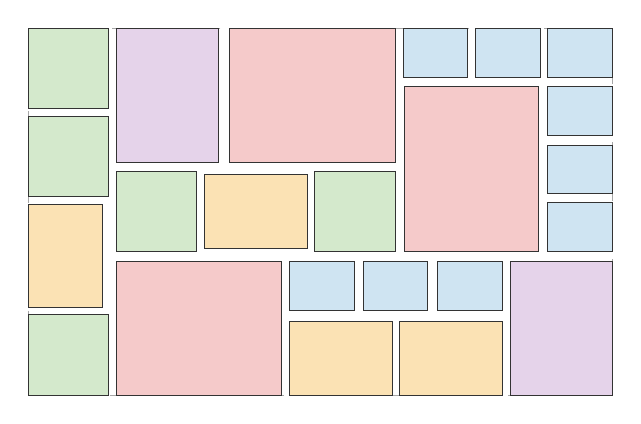
\begin{tikzpicture}[x=0.4mm, y=-0.4mm]
\draw[gray!70, dashed, line width=0.4pt] (0,0) rectangle (185.50,116.50);
\filldraw[fill=ft2, draw=black!80, line width=0.3pt] (0.00,0.00) rectangle (25.50,25.50);
\filldraw[fill=ft3, draw=black!80, line width=0.3pt] (28.00,0.00) rectangle (60.50,42.50);
\filldraw[fill=ft4, draw=black!80, line width=0.3pt] (64.00,0.00) rectangle (116.50,42.50);
\filldraw[fill=ft0, draw=black!80, line width=0.3pt] (119.00,0.00) rectangle (139.50,15.50);
\filldraw[fill=ft0, draw=black!80, line width=0.3pt] (142.00,0.00) rectangle (162.50,15.50);
\filldraw[fill=ft0, draw=black!80, line width=0.3pt] (165.00,0.00) rectangle (185.50,15.50);
\filldraw[fill=ft4, draw=black!80, line width=0.3pt] (119.50,18.38) rectangle (162.00,70.88);
\filldraw[fill=ft0, draw=black!80, line width=0.3pt] (165.00,18.63) rectangle (185.50,34.13);
\filldraw[fill=ft2, draw=black!80, line width=0.3pt] (0.00,28.00) rectangle (25.50,53.50);
\filldraw[fill=ft0, draw=black!80, line width=0.3pt] (165.00,37.09) rectangle (185.50,52.59);
\filldraw[fill=ft2, draw=black!80, line width=0.3pt] (28.00,45.38) rectangle (53.50,70.88);
\filldraw[fill=ft2, draw=black!80, line width=0.3pt] (91.00,45.38) rectangle (116.50,70.88);
\filldraw[fill=ft1, draw=black!80, line width=0.3pt] (56.00,46.38) rectangle (88.50,69.88);
\filldraw[fill=ft0, draw=black!80, line width=0.3pt] (165.00,55.38) rectangle (185.50,70.88);
\filldraw[fill=ft1, draw=black!80, line width=0.3pt] (0.00,56.00) rectangle (23.50,88.50);
\filldraw[fill=ft4, draw=black!80, line width=0.3pt] (28.00,74.00) rectangle (80.50,116.50);
\filldraw[fill=ft0, draw=black!80, line width=0.3pt] (83.00,74.00) rectangle (103.50,89.50);
\filldraw[fill=ft0, draw=black!80, line width=0.3pt] (106.39,74.00) rectangle (126.89,89.50);
\filldraw[fill=ft0, draw=black!80, line width=0.3pt] (130.00,74.00) rectangle (150.50,89.50);
\filldraw[fill=ft3, draw=black!80, line width=0.3pt] (153.00,74.00) rectangle (185.50,116.50);
\filldraw[fill=ft2, draw=black!80, line width=0.3pt] (0.00,91.00) rectangle (25.50,116.50);
\filldraw[fill=ft1, draw=black!80, line width=0.3pt] (83.00,93.00) rectangle (115.50,116.50);
\filldraw[fill=ft1, draw=black!80, line width=0.3pt] (118.00,93.00) rectangle (150.50,116.50);
\end{tikzpicture}\\[2pt]
{\small\bfseries proportional} -- \hyperref[lay:proportional:1]{layout 1}\\
{\scriptsize 185.5 $\times$ 116.5 cm, 23 frames, gap 2.5 cm,
max.\ dev.\ 2.0 cm, notches none, entropy 0.77}
\end{minipage}
\par\vspace{10pt}
\begin{minipage}[t]{0.32\textwidth}\centering\vspace{0pt}
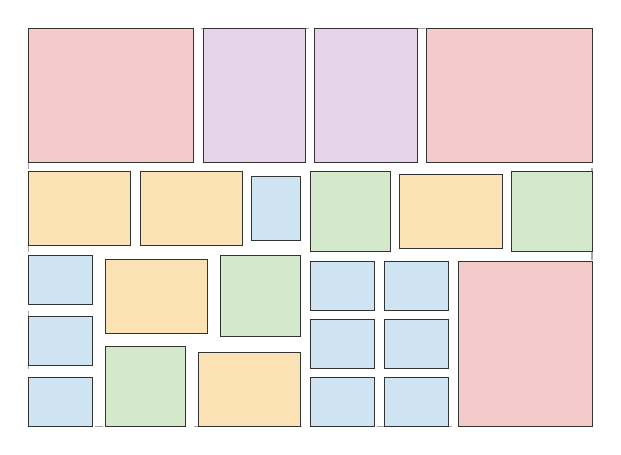
\begin{tikzpicture}[x=0.4mm, y=-0.4mm]
\draw[gray!70, dashed, line width=0.4pt] (0,0) rectangle (179.00,126.50);
\filldraw[fill=ft4, draw=black!80, line width=0.3pt] (0.00,0.00) rectangle (52.50,42.50);
\filldraw[fill=ft3, draw=black!80, line width=0.3pt] (55.50,0.00) rectangle (88.00,42.50);
\filldraw[fill=ft3, draw=black!80, line width=0.3pt] (91.00,0.00) rectangle (123.50,42.50);
\filldraw[fill=ft4, draw=black!80, line width=0.3pt] (126.50,0.00) rectangle (179.00,42.50);
\filldraw[fill=ft1, draw=black!80, line width=0.3pt] (0.00,45.50) rectangle (32.50,69.00);
\filldraw[fill=ft1, draw=black!80, line width=0.3pt] (35.50,45.50) rectangle (68.00,69.00);
\filldraw[fill=ft2, draw=black!80, line width=0.3pt] (89.50,45.50) rectangle (115.00,71.00);
\filldraw[fill=ft2, draw=black!80, line width=0.3pt] (153.50,45.50) rectangle (179.00,71.00);
\filldraw[fill=ft1, draw=black!80, line width=0.3pt] (118.00,46.50) rectangle (150.50,70.00);
\filldraw[fill=ft0, draw=black!80, line width=0.3pt] (71.00,47.00) rectangle (86.50,67.50);
\filldraw[fill=ft0, draw=black!80, line width=0.3pt] (0.00,72.25) rectangle (20.50,87.75);
\filldraw[fill=ft2, draw=black!80, line width=0.3pt] (61.00,72.25) rectangle (86.50,97.75);
\filldraw[fill=ft1, draw=black!80, line width=0.3pt] (24.50,73.25) rectangle (57.00,96.75);
\filldraw[fill=ft0, draw=black!80, line width=0.3pt] (89.50,74.00) rectangle (110.00,89.50);
\filldraw[fill=ft0, draw=black!80, line width=0.3pt] (113.00,74.00) rectangle (133.50,89.50);
\filldraw[fill=ft4, draw=black!80, line width=0.3pt] (136.50,74.00) rectangle (179.00,126.50);
\filldraw[fill=ft0, draw=black!80, line width=0.3pt] (0.00,91.62) rectangle (20.50,107.12);
\filldraw[fill=ft0, draw=black!80, line width=0.3pt] (89.50,92.50) rectangle (110.00,108.00);
\filldraw[fill=ft0, draw=black!80, line width=0.3pt] (113.00,92.50) rectangle (133.50,108.00);
\filldraw[fill=ft2, draw=black!80, line width=0.3pt] (24.50,101.00) rectangle (50.00,126.50);
\filldraw[fill=ft1, draw=black!80, line width=0.3pt] (54.00,103.00) rectangle (86.50,126.50);
\filldraw[fill=ft0, draw=black!80, line width=0.3pt] (0.00,111.00) rectangle (20.50,126.50);
\filldraw[fill=ft0, draw=black!80, line width=0.3pt] (89.50,111.00) rectangle (110.00,126.50);
\filldraw[fill=ft0, draw=black!80, line width=0.3pt] (113.00,111.00) rectangle (133.50,126.50);
\end{tikzpicture}\\[2pt]
{\small\bfseries gap-3} -- \hyperref[lay:gap-3:1]{layout 1}\\
{\scriptsize 179.0 $\times$ 126.5 cm, 24 frames, gap 3 cm,
max.\ dev.\ 2.2 cm, notches none, entropy 0.64}
\end{minipage}\hfill
\begin{minipage}[t]{0.32\textwidth}\centering\vspace{0pt}
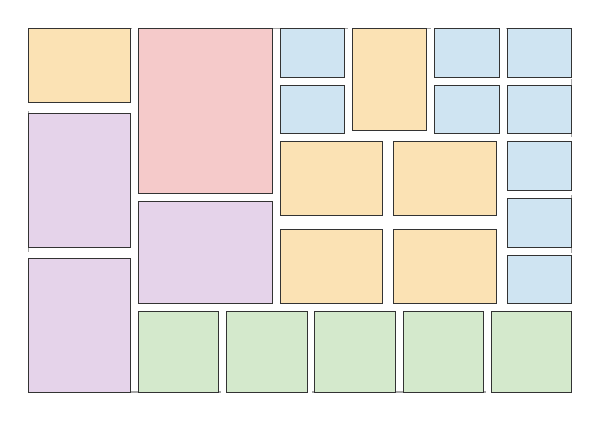
\begin{tikzpicture}[x=0.4mm, y=-0.4mm]
\draw[gray!70, dashed, line width=0.4pt] (0,0) rectangle (172.50,115.50);
\filldraw[fill=ft1, draw=black!80, line width=0.3pt] (0.00,0.00) rectangle (32.50,23.50);
\filldraw[fill=ft4, draw=black!80, line width=0.3pt] (35.00,0.00) rectangle (77.50,52.50);
\filldraw[fill=ft0, draw=black!80, line width=0.3pt] (80.00,0.00) rectangle (100.50,15.50);
\filldraw[fill=ft1, draw=black!80, line width=0.3pt] (103.00,0.00) rectangle (126.50,32.50);
\filldraw[fill=ft0, draw=black!80, line width=0.3pt] (129.00,0.00) rectangle (149.50,15.50);
\filldraw[fill=ft0, draw=black!80, line width=0.3pt] (152.00,0.00) rectangle (172.50,15.50);
\filldraw[fill=ft0, draw=black!80, line width=0.3pt] (80.00,18.00) rectangle (100.50,33.50);
\filldraw[fill=ft0, draw=black!80, line width=0.3pt] (129.00,18.00) rectangle (149.50,33.50);
\filldraw[fill=ft0, draw=black!80, line width=0.3pt] (152.00,18.00) rectangle (172.50,33.50);
\filldraw[fill=ft3, draw=black!80, line width=0.3pt] (0.00,27.00) rectangle (32.50,69.50);
\filldraw[fill=ft1, draw=black!80, line width=0.3pt] (80.00,36.00) rectangle (112.50,59.50);
\filldraw[fill=ft1, draw=black!80, line width=0.3pt] (116.00,36.00) rectangle (148.50,59.50);
\filldraw[fill=ft0, draw=black!80, line width=0.3pt] (152.00,36.00) rectangle (172.50,51.50);
\filldraw[fill=ft0, draw=black!80, line width=0.3pt] (152.00,54.00) rectangle (172.50,69.50);
\filldraw[fill=ft3, draw=black!80, line width=0.3pt] (35.00,55.00) rectangle (77.50,87.50);
\filldraw[fill=ft1, draw=black!80, line width=0.3pt] (80.00,64.00) rectangle (112.50,87.50);
\filldraw[fill=ft1, draw=black!80, line width=0.3pt] (116.00,64.00) rectangle (148.50,87.50);
\filldraw[fill=ft0, draw=black!80, line width=0.3pt] (152.00,72.00) rectangle (172.50,87.50);
\filldraw[fill=ft3, draw=black!80, line width=0.3pt] (0.00,73.00) rectangle (32.50,115.50);
\filldraw[fill=ft2, draw=black!80, line width=0.3pt] (35.00,90.00) rectangle (60.50,115.50);
\filldraw[fill=ft2, draw=black!80, line width=0.3pt] (63.00,90.00) rectangle (88.50,115.50);
\filldraw[fill=ft2, draw=black!80, line width=0.3pt] (91.00,90.00) rectangle (116.50,115.50);
\filldraw[fill=ft2, draw=black!80, line width=0.3pt] (119.00,90.00) rectangle (144.50,115.50);
\filldraw[fill=ft2, draw=black!80, line width=0.3pt] (147.00,90.00) rectangle (172.50,115.50);
\end{tikzpicture}\\[2pt]
{\small\bfseries linear-cost} -- \hyperref[lay:linear-cost:1]{layout 1}\\
{\scriptsize 172.5 $\times$ 115.5 cm, 24 frames, gap 2.5 cm,
max.\ dev.\ 2.0 cm, notches none, entropy 0.71}
\end{minipage}\hfill
\begin{minipage}[t]{0.32\textwidth}\centering\vspace{0pt}
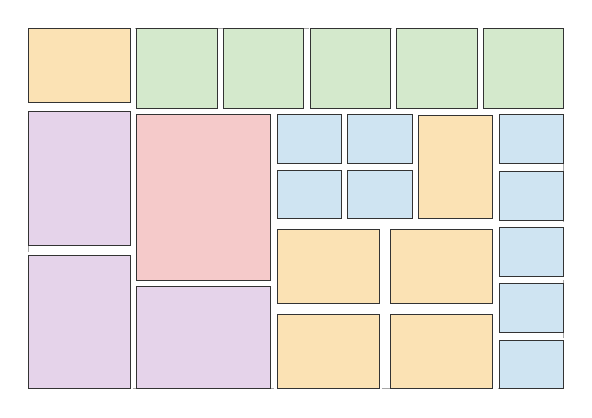
\begin{tikzpicture}[x=0.4mm, y=-0.4mm]
\draw[gray!70, dashed, line width=0.4pt] (0,0) rectangle (170.00,114.50);
\filldraw[fill=ft1, draw=black!80, line width=0.3pt] (0.00,0.00) rectangle (32.50,23.50);
\filldraw[fill=ft2, draw=black!80, line width=0.3pt] (34.50,0.00) rectangle (60.00,25.50);
\filldraw[fill=ft2, draw=black!80, line width=0.3pt] (62.00,0.00) rectangle (87.50,25.50);
\filldraw[fill=ft2, draw=black!80, line width=0.3pt] (89.50,0.00) rectangle (115.00,25.50);
\filldraw[fill=ft2, draw=black!80, line width=0.3pt] (117.00,0.00) rectangle (142.50,25.50);
\filldraw[fill=ft2, draw=black!80, line width=0.3pt] (144.50,0.00) rectangle (170.00,25.50);
\filldraw[fill=ft3, draw=black!80, line width=0.3pt] (0.00,26.50) rectangle (32.50,69.00);
\filldraw[fill=ft4, draw=black!80, line width=0.3pt] (34.50,27.50) rectangle (77.00,80.00);
\filldraw[fill=ft0, draw=black!80, line width=0.3pt] (79.00,27.50) rectangle (99.50,43.00);
\filldraw[fill=ft0, draw=black!80, line width=0.3pt] (101.50,27.50) rectangle (122.00,43.00);
\filldraw[fill=ft0, draw=black!80, line width=0.3pt] (149.50,27.50) rectangle (170.00,43.00);
\filldraw[fill=ft1, draw=black!80, line width=0.3pt] (124.00,27.75) rectangle (147.50,60.25);
\filldraw[fill=ft0, draw=black!80, line width=0.3pt] (79.00,45.00) rectangle (99.50,60.50);
\filldraw[fill=ft0, draw=black!80, line width=0.3pt] (101.50,45.00) rectangle (122.00,60.50);
\filldraw[fill=ft0, draw=black!80, line width=0.3pt] (149.50,45.38) rectangle (170.00,60.88);
\filldraw[fill=ft0, draw=black!80, line width=0.3pt] (149.50,63.25) rectangle (170.00,78.75);
\filldraw[fill=ft1, draw=black!80, line width=0.3pt] (79.00,64.00) rectangle (111.50,87.50);
\filldraw[fill=ft1, draw=black!80, line width=0.3pt] (115.00,64.00) rectangle (147.50,87.50);
\filldraw[fill=ft3, draw=black!80, line width=0.3pt] (0.00,72.00) rectangle (32.50,114.50);
\filldraw[fill=ft0, draw=black!80, line width=0.3pt] (149.50,81.12) rectangle (170.00,96.62);
\filldraw[fill=ft3, draw=black!80, line width=0.3pt] (34.50,82.00) rectangle (77.00,114.50);
\filldraw[fill=ft1, draw=black!80, line width=0.3pt] (79.00,91.00) rectangle (111.50,114.50);
\filldraw[fill=ft1, draw=black!80, line width=0.3pt] (115.00,91.00) rectangle (147.50,114.50);
\filldraw[fill=ft0, draw=black!80, line width=0.3pt] (149.50,99.00) rectangle (170.00,114.50);
\end{tikzpicture}\\[2pt]
{\small\bfseries free-gap-s1} -- \hyperref[lay:free-gap-s1:1]{layout 1}\\
{\scriptsize 170.0 $\times$ 114.5 cm, 24 frames, gap 2 cm,
max.\ dev.\ 1.8 cm, notches 4 cm, entropy 0.66}
\end{minipage}
\par\vspace{10pt}
\begin{minipage}[t]{0.32\textwidth}\centering\vspace{0pt}
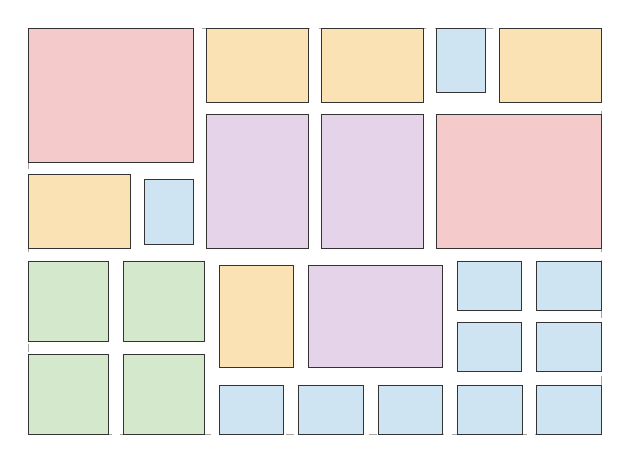
\begin{tikzpicture}[x=0.4mm, y=-0.4mm]
\draw[gray!70, dashed, line width=0.4pt] (0,0) rectangle (182.00,129.00);
\filldraw[fill=ft4, draw=black!80, line width=0.3pt] (0.00,0.00) rectangle (52.50,42.50);
\filldraw[fill=ft1, draw=black!80, line width=0.3pt] (56.50,0.00) rectangle (89.00,23.50);
\filldraw[fill=ft1, draw=black!80, line width=0.3pt] (93.00,0.00) rectangle (125.50,23.50);
\filldraw[fill=ft0, draw=black!80, line width=0.3pt] (129.50,0.00) rectangle (145.00,20.50);
\filldraw[fill=ft1, draw=black!80, line width=0.3pt] (149.50,0.00) rectangle (182.00,23.50);
\filldraw[fill=ft3, draw=black!80, line width=0.3pt] (56.50,27.50) rectangle (89.00,70.00);
\filldraw[fill=ft3, draw=black!80, line width=0.3pt] (93.00,27.50) rectangle (125.50,70.00);
\filldraw[fill=ft4, draw=black!80, line width=0.3pt] (129.50,27.50) rectangle (182.00,70.00);
\filldraw[fill=ft1, draw=black!80, line width=0.3pt] (0.00,46.50) rectangle (32.50,70.00);
\filldraw[fill=ft0, draw=black!80, line width=0.3pt] (37.00,48.00) rectangle (52.50,68.50);
\filldraw[fill=ft2, draw=black!80, line width=0.3pt] (0.00,74.00) rectangle (25.50,99.50);
\filldraw[fill=ft2, draw=black!80, line width=0.3pt] (30.30,74.00) rectangle (55.80,99.50);
\filldraw[fill=ft0, draw=black!80, line width=0.3pt] (136.20,74.00) rectangle (156.70,89.50);
\filldraw[fill=ft0, draw=black!80, line width=0.3pt] (161.50,74.00) rectangle (182.00,89.50);
\filldraw[fill=ft1, draw=black!80, line width=0.3pt] (60.60,75.25) rectangle (84.10,107.75);
\filldraw[fill=ft3, draw=black!80, line width=0.3pt] (88.90,75.25) rectangle (131.40,107.75);
\filldraw[fill=ft0, draw=black!80, line width=0.3pt] (136.20,93.50) rectangle (156.70,109.00);
\filldraw[fill=ft0, draw=black!80, line width=0.3pt] (161.50,93.50) rectangle (182.00,109.00);
\filldraw[fill=ft2, draw=black!80, line width=0.3pt] (0.00,103.50) rectangle (25.50,129.00);
\filldraw[fill=ft2, draw=black!80, line width=0.3pt] (30.30,103.50) rectangle (55.80,129.00);
\filldraw[fill=ft0, draw=black!80, line width=0.3pt] (60.60,113.50) rectangle (81.10,129.00);
\filldraw[fill=ft0, draw=black!80, line width=0.3pt] (85.82,113.50) rectangle (106.32,129.00);
\filldraw[fill=ft0, draw=black!80, line width=0.3pt] (111.05,113.50) rectangle (131.55,129.00);
\filldraw[fill=ft0, draw=black!80, line width=0.3pt] (136.27,113.50) rectangle (156.77,129.00);
\filldraw[fill=ft0, draw=black!80, line width=0.3pt] (161.50,113.50) rectangle (182.00,129.00);
\end{tikzpicture}\\[2pt]
{\small\bfseries large-apart} -- \hyperref[lay:large-apart:1]{layout 1}\\
{\scriptsize 182.0 $\times$ 129.0 cm, 25 frames, gap 4 cm,
max.\ dev.\ 3.0 cm, notches none, entropy 0.65}
\end{minipage}\hfill
\begin{minipage}[t]{0.32\textwidth}\centering\vspace{0pt}
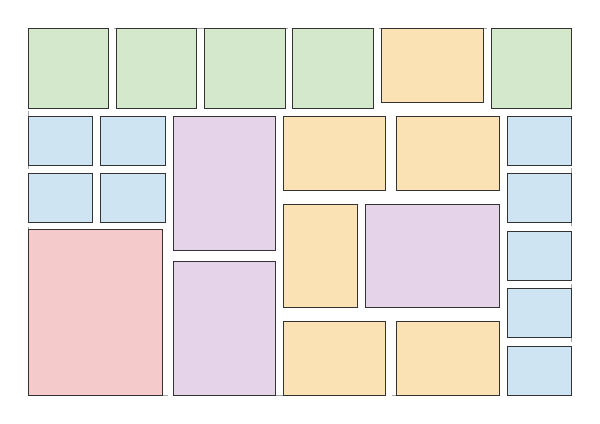
\begin{tikzpicture}[x=0.4mm, y=-0.4mm]
\draw[gray!70, dashed, line width=0.4pt] (0,0) rectangle (172.50,116.50);
\filldraw[fill=ft2, draw=black!80, line width=0.3pt] (0.00,0.00) rectangle (25.50,25.50);
\filldraw[fill=ft2, draw=black!80, line width=0.3pt] (28.00,0.00) rectangle (53.50,25.50);
\filldraw[fill=ft2, draw=black!80, line width=0.3pt] (56.00,0.00) rectangle (81.50,25.50);
\filldraw[fill=ft2, draw=black!80, line width=0.3pt] (84.00,0.00) rectangle (109.50,25.50);
\filldraw[fill=ft1, draw=black!80, line width=0.3pt] (112.00,0.00) rectangle (144.50,23.50);
\filldraw[fill=ft2, draw=black!80, line width=0.3pt] (147.00,0.00) rectangle (172.50,25.50);
\filldraw[fill=ft0, draw=black!80, line width=0.3pt] (0.00,28.00) rectangle (20.50,43.50);
\filldraw[fill=ft0, draw=black!80, line width=0.3pt] (23.00,28.00) rectangle (43.50,43.50);
\filldraw[fill=ft3, draw=black!80, line width=0.3pt] (46.00,28.00) rectangle (78.50,70.50);
\filldraw[fill=ft1, draw=black!80, line width=0.3pt] (81.00,28.00) rectangle (113.50,51.50);
\filldraw[fill=ft1, draw=black!80, line width=0.3pt] (117.00,28.00) rectangle (149.50,51.50);
\filldraw[fill=ft0, draw=black!80, line width=0.3pt] (152.00,28.00) rectangle (172.50,43.50);
\filldraw[fill=ft0, draw=black!80, line width=0.3pt] (0.00,46.00) rectangle (20.50,61.50);
\filldraw[fill=ft0, draw=black!80, line width=0.3pt] (23.00,46.00) rectangle (43.50,61.50);
\filldraw[fill=ft0, draw=black!80, line width=0.3pt] (152.00,46.25) rectangle (172.50,61.75);
\filldraw[fill=ft1, draw=black!80, line width=0.3pt] (81.00,56.00) rectangle (104.50,88.50);
\filldraw[fill=ft3, draw=black!80, line width=0.3pt] (107.00,56.00) rectangle (149.50,88.50);
\filldraw[fill=ft4, draw=black!80, line width=0.3pt] (0.00,64.00) rectangle (42.50,116.50);
\filldraw[fill=ft0, draw=black!80, line width=0.3pt] (152.00,64.50) rectangle (172.50,80.00);
\filldraw[fill=ft3, draw=black!80, line width=0.3pt] (46.00,74.00) rectangle (78.50,116.50);
\filldraw[fill=ft0, draw=black!80, line width=0.3pt] (152.00,82.75) rectangle (172.50,98.25);
\filldraw[fill=ft1, draw=black!80, line width=0.3pt] (81.00,93.00) rectangle (113.50,116.50);
\filldraw[fill=ft1, draw=black!80, line width=0.3pt] (117.00,93.00) rectangle (149.50,116.50);
\filldraw[fill=ft0, draw=black!80, line width=0.3pt] (152.00,101.00) rectangle (172.50,116.50);
\end{tikzpicture}\\[2pt]
{\small\bfseries entropy} -- \hyperref[lay:entropy:1]{layout 1}\\
{\scriptsize 172.5 $\times$ 116.5 cm, 24 frames, gap 2.5 cm,
max.\ dev.\ 2.0 cm, notches none, entropy 0.72}
\end{minipage}\hfill
\begin{minipage}[t]{0.32\textwidth}\centering\vspace{0pt}
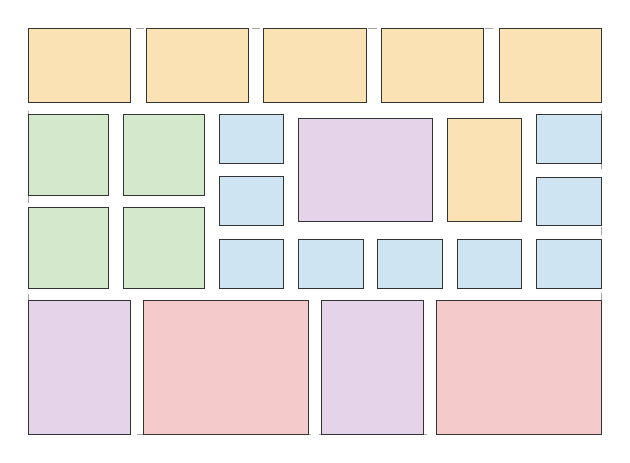
\begin{tikzpicture}[x=0.4mm, y=-0.4mm]
\draw[gray!70, dashed, line width=0.4pt] (0,0) rectangle (182.00,129.00);
\filldraw[fill=ft1, draw=black!80, line width=0.3pt] (0.00,0.00) rectangle (32.50,23.50);
\filldraw[fill=ft1, draw=black!80, line width=0.3pt] (37.38,0.00) rectangle (69.88,23.50);
\filldraw[fill=ft1, draw=black!80, line width=0.3pt] (74.75,0.00) rectangle (107.25,23.50);
\filldraw[fill=ft1, draw=black!80, line width=0.3pt] (112.12,0.00) rectangle (144.62,23.50);
\filldraw[fill=ft1, draw=black!80, line width=0.3pt] (149.50,0.00) rectangle (182.00,23.50);
\filldraw[fill=ft2, draw=black!80, line width=0.3pt] (0.00,27.50) rectangle (25.50,53.00);
\filldraw[fill=ft2, draw=black!80, line width=0.3pt] (30.30,27.50) rectangle (55.80,53.00);
\filldraw[fill=ft0, draw=black!80, line width=0.3pt] (60.60,27.50) rectangle (81.10,43.00);
\filldraw[fill=ft0, draw=black!80, line width=0.3pt] (161.50,27.50) rectangle (182.00,43.00);
\filldraw[fill=ft3, draw=black!80, line width=0.3pt] (85.90,28.75) rectangle (128.40,61.25);
\filldraw[fill=ft1, draw=black!80, line width=0.3pt] (133.20,28.75) rectangle (156.70,61.25);
\filldraw[fill=ft0, draw=black!80, line width=0.3pt] (60.60,47.00) rectangle (81.10,62.50);
\filldraw[fill=ft0, draw=black!80, line width=0.3pt] (161.50,47.25) rectangle (182.00,62.75);
\filldraw[fill=ft2, draw=black!80, line width=0.3pt] (0.00,57.00) rectangle (25.50,82.50);
\filldraw[fill=ft2, draw=black!80, line width=0.3pt] (30.30,57.00) rectangle (55.80,82.50);
\filldraw[fill=ft0, draw=black!80, line width=0.3pt] (60.60,67.00) rectangle (81.10,82.50);
\filldraw[fill=ft0, draw=black!80, line width=0.3pt] (85.80,67.00) rectangle (106.30,82.50);
\filldraw[fill=ft0, draw=black!80, line width=0.3pt] (111.00,67.00) rectangle (131.50,82.50);
\filldraw[fill=ft0, draw=black!80, line width=0.3pt] (136.20,67.00) rectangle (156.70,82.50);
\filldraw[fill=ft0, draw=black!80, line width=0.3pt] (161.50,67.00) rectangle (182.00,82.50);
\filldraw[fill=ft3, draw=black!80, line width=0.3pt] (0.00,86.50) rectangle (32.50,129.00);
\filldraw[fill=ft4, draw=black!80, line width=0.3pt] (36.50,86.50) rectangle (89.00,129.00);
\filldraw[fill=ft3, draw=black!80, line width=0.3pt] (93.00,86.50) rectangle (125.50,129.00);
\filldraw[fill=ft4, draw=black!80, line width=0.3pt] (129.50,86.50) rectangle (182.00,129.00);
\end{tikzpicture}\\[2pt]
{\small\bfseries large-entropy} -- \hyperref[lay:large-entropy:1]{layout 1}\\
{\scriptsize 182.0 $\times$ 129.0 cm, 24 frames, gap 4 cm,
max.\ dev.\ 1.8 cm, notches none, entropy 0.65}
\end{minipage}
\par\vspace{10pt}
\clearpage

\section{Combined ranking}\label{sec:combined}
The 144 layouts shown in this document (144 distinct ones; a layout found by several paradigms is
listed once, with the other paradigms in the third column) ranked together by the same score (gap uniformity and
border only; the sub-analysis constraints are not part of this score). Click a layout to jump to its page.\\[8pt]
\begin{tabular}{@{}r l l l r r r r l c r r@{}}
\toprule
\# & paradigm / layout & also found by & size (cm) & gap & frames & max dev & mean dev & notches & corners & entropy & score \\
\midrule
1 & \hyperref[lay:free-gap:1]{free-gap / 1} & {\small --} & 181.5 $\times$ 113.5 & 1.5 & 20 & 1.0 & 0.59 & none & 4/4 & 0.71 & 1.29 \\
2 & \hyperref[lay:free-gap:2]{free-gap / 2} & {\small --} & 182.0 $\times$ 129.0 & 4 & 24 & 1.8 & 0.53 & none & 4/4 & 0.64 & 2.01 \\
3 & \hyperref[lay:large-entropy:1]{large-entropy / 1} & {\small --} & 182.0 $\times$ 129.0 & 4 & 24 & 1.8 & 0.56 & none & 4/4 & 0.65 & 2.03 \\
4 & \hyperref[lay:linear-cost:1]{linear-cost / 1} & {\small --} & 172.5 $\times$ 115.5 & 2.5 & 24 & 2.0 & 0.30 & none & 4/4 & 0.71 & 2.15 \\
5 & \hyperref[lay:entropy:1]{entropy / 1} & {\small --} & 172.5 $\times$ 116.5 & 2.5 & 24 & 2.0 & 0.43 & none & 4/4 & 0.72 & 2.21 \\
6 & \hyperref[lay:free-gap-s1:1]{free-gap-s1 / 1} & {\small --} & 170.0 $\times$ 114.5 & 2 & 24 & 1.8 & 0.33 & 4 cm & 4/4 & 0.66 & 2.44 \\
7 & \hyperref[lay:free-gap-s1:2]{free-gap-s1 / 2} & {\small --} & 170.0 $\times$ 114.5 & 2 & 24 & 1.8 & 0.35 & 4 cm & 4/4 & 0.71 & 2.45 \\
8 & \hyperref[lay:gap-3:1]{gap-3 / 1} & {\small --} & 179.0 $\times$ 126.5 & 3 & 24 & 2.2 & 0.44 & none & 4/4 & 0.64 & 2.47 \\
9 & \hyperref[lay:proportional:1]{proportional / 1} & {\small --} & 185.5 $\times$ 116.5 & 2.5 & 23 & 2.0 & 0.51 & none & 4/4 & 0.77 & 2.25 \\
10 & \hyperref[lay:linear-cost:2]{linear-cost / 2} & {\small --} & 181.5 $\times$ 113.5 & 1.5 & 23 & 2.0 & 0.52 & none & 4/4 & 0.57 & 2.26 \\
11 & \hyperref[lay:linear-cost:3]{linear-cost / 3} & {\small --} & 181.5 $\times$ 113.5 & 1.5 & 23 & 2.0 & 0.53 & none & 4/4 & 0.72 & 2.27 \\
12 & \hyperref[lay:free-gap:3]{free-gap / 3} & {\small --} & 184.0 $\times$ 115.0 & 2 & 23 & 2.0 & 0.56 & none & 4/4 & 0.76 & 2.28 \\
13 & \hyperref[lay:free-gap-s1:3]{free-gap-s1 / 3} & {\small --} & 184.0 $\times$ 115.0 & 2 & 23 & 2.0 & 0.57 & none & 4/4 & 0.74 & 2.29 \\
14 & \hyperref[lay:proportional:2]{proportional / 2} & {\small --} & 184.0 $\times$ 115.0 & 2 & 23 & 2.0 & 0.57 & none & 4/4 & 0.69 & 2.29 \\
15 & \hyperref[lay:free-gap-s1:4]{free-gap-s1 / 4} & {\small --} & 183.5 $\times$ 115.0 & 2 & 23 & 2.2 & 0.48 & none & 4/4 & 0.76 & 2.49 \\
16 & \hyperref[lay:free-gap-s1:5]{free-gap-s1 / 5} & {\small --} & 190.5 $\times$ 115.5 & 2.5 & 22 & 2.0 & 0.41 & none & 4/4 & 0.68 & 2.20 \\
17 & \hyperref[lay:linear-cost:4]{linear-cost / 4} & {\small --} & 189.5 $\times$ 109.5 & 3.5 & 22 & 2.0 & 0.40 & none & 4/4 & 0.76 & 2.20 \\
18 & \hyperref[lay:free-gap-s1:6]{free-gap-s1 / 6} & {\small --} & 171.5 $\times$ 116.5 & 2.5 & 22 & 2.0 & 0.61 & none & 4/4 & 0.74 & 2.30 \\
19 & \hyperref[lay:free-gap:4]{free-gap / 4} & {\small --} & 177.5 $\times$ 113.5 & 1.5 & 21 & 2.0 & 0.51 & none & 4/4 & 0.66 & 2.26 \\
20 & \hyperref[lay:linear-cost:5]{linear-cost / 5} & {\small --} & 181.5 $\times$ 113.5 & 1.5 & 20 & 2.0 & 0.55 & none & 4/4 & 0.78 & 2.28 \\
\bottomrule
\end{tabular}
\clearpage

\section{Sub-analysis: large frames apart, entropy}\label{sec:sub}
The following paradigms add constraints on top of the baseline search:
\hyperref[sec:large-apart]{large-apart}, \hyperref[sec:entropy]{entropy}, \hyperref[sec:large-entropy]{large-entropy}. The gap and border measures stay the
same; the extra measures are shown on every layout page and in the tables below.

\vspace{4pt}
{\bfseries Large frames apart.} Frames with an outer area of at least 2000 cm$^2$ count
as large (here the 52.5 $\times$ 42.5 and 42.5 $\times$ 52.5 frames). The layout must contain between
2 and 3 of them (each one missing or too many costs as much as a 1.5 cm notch across the whole
width). Two large frames that face each other across a regular gap are ``touching''; the penalty grows with the
edge they share, so barely touching is almost free. In addition the closest pair of large frames is pulled towards a
centre distance of at least 70 cm. The tables report the number of large frames, how many pairs touch
(with the total shared edge) and the smallest centre distance.

\vspace{4pt}
{\bfseries Entropy.} A number in $[0, 1]$ for how irregular (``random'') a constellation looks, the
mean of four shares: \emph{mix} -- the Shannon entropy of the formats used, relative to using all formats equally;
\emph{variety} -- the share of neighbouring pairs (across a regular gap) that have different formats;
\emph{stagger} -- the share of distinct frame edge positions (in a grid most edges line up, so it scores low);
\emph{lines} -- 1 for a single straight gap line running across the whole collage, 0 for five or more.
The search adds $w \cdot (1 - \mathrm{entropy})$ to the cost, so it trades a little gap uniformity for irregularity;
layouts with equal rounded score are ranked by entropy.

\vspace{10pt}
{\bfseries Best-ranked layout of each sub-analysis paradigm} (cm; large = count, touching pairs, min.\ centre distance;
entropy components = mix / variety / stagger / lines)\\[4pt]
\begin{tabular}{@{}l r l r r r l l r l r@{}}
\toprule
paradigm & layout & size & frames & gap & max dev & notches & large frames & entropy & components & score \\
\midrule
\hyperref[sec:large-apart]{large-apart} & \hyperref[lay:large-apart:1]{1} & 182.0 $\times$ 129.0 & 25 & 4 & 3.0 & none & 2, apart, 132 cm & 0.65 & 0.83 / 0.54 / 0.48 / 0.75 & 3.30 \\
\hyperref[sec:entropy]{entropy} & \hyperref[lay:entropy:1]{1} & 172.5 $\times$ 116.5 & 24 & 2.5 & 2.0 & none & 1 & 0.72 & 0.74 / 0.65 / 0.49 / 1.00 & 2.21 \\
\hyperref[sec:large-entropy]{large-entropy} & \hyperref[lay:large-entropy:1]{1} & 182.0 $\times$ 129.0 & 24 & 4 & 1.8 & none & 2, apart, 93 cm & 0.65 & 0.76 / 0.60 / 0.48 / 0.75 & 2.03 \\
\bottomrule
\end{tabular}
\clearpage
{\large\bfseries Best-ranked layout of each sub-analysis paradigm at a glance} {\small (scale 1:25)}\\[10pt]
\begin{minipage}[t]{0.32\textwidth}\centering\vspace{0pt}
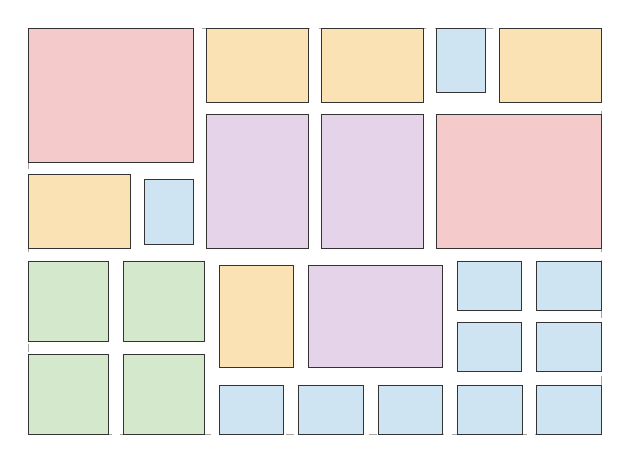
\begin{tikzpicture}[x=0.4mm, y=-0.4mm]
\draw[gray!70, dashed, line width=0.4pt] (0,0) rectangle (182.00,129.00);
\filldraw[fill=ft4, draw=black!80, line width=0.3pt] (0.00,0.00) rectangle (52.50,42.50);
\filldraw[fill=ft1, draw=black!80, line width=0.3pt] (56.50,0.00) rectangle (89.00,23.50);
\filldraw[fill=ft1, draw=black!80, line width=0.3pt] (93.00,0.00) rectangle (125.50,23.50);
\filldraw[fill=ft0, draw=black!80, line width=0.3pt] (129.50,0.00) rectangle (145.00,20.50);
\filldraw[fill=ft1, draw=black!80, line width=0.3pt] (149.50,0.00) rectangle (182.00,23.50);
\filldraw[fill=ft3, draw=black!80, line width=0.3pt] (56.50,27.50) rectangle (89.00,70.00);
\filldraw[fill=ft3, draw=black!80, line width=0.3pt] (93.00,27.50) rectangle (125.50,70.00);
\filldraw[fill=ft4, draw=black!80, line width=0.3pt] (129.50,27.50) rectangle (182.00,70.00);
\filldraw[fill=ft1, draw=black!80, line width=0.3pt] (0.00,46.50) rectangle (32.50,70.00);
\filldraw[fill=ft0, draw=black!80, line width=0.3pt] (37.00,48.00) rectangle (52.50,68.50);
\filldraw[fill=ft2, draw=black!80, line width=0.3pt] (0.00,74.00) rectangle (25.50,99.50);
\filldraw[fill=ft2, draw=black!80, line width=0.3pt] (30.30,74.00) rectangle (55.80,99.50);
\filldraw[fill=ft0, draw=black!80, line width=0.3pt] (136.20,74.00) rectangle (156.70,89.50);
\filldraw[fill=ft0, draw=black!80, line width=0.3pt] (161.50,74.00) rectangle (182.00,89.50);
\filldraw[fill=ft1, draw=black!80, line width=0.3pt] (60.60,75.25) rectangle (84.10,107.75);
\filldraw[fill=ft3, draw=black!80, line width=0.3pt] (88.90,75.25) rectangle (131.40,107.75);
\filldraw[fill=ft0, draw=black!80, line width=0.3pt] (136.20,93.50) rectangle (156.70,109.00);
\filldraw[fill=ft0, draw=black!80, line width=0.3pt] (161.50,93.50) rectangle (182.00,109.00);
\filldraw[fill=ft2, draw=black!80, line width=0.3pt] (0.00,103.50) rectangle (25.50,129.00);
\filldraw[fill=ft2, draw=black!80, line width=0.3pt] (30.30,103.50) rectangle (55.80,129.00);
\filldraw[fill=ft0, draw=black!80, line width=0.3pt] (60.60,113.50) rectangle (81.10,129.00);
\filldraw[fill=ft0, draw=black!80, line width=0.3pt] (85.82,113.50) rectangle (106.32,129.00);
\filldraw[fill=ft0, draw=black!80, line width=0.3pt] (111.05,113.50) rectangle (131.55,129.00);
\filldraw[fill=ft0, draw=black!80, line width=0.3pt] (136.27,113.50) rectangle (156.77,129.00);
\filldraw[fill=ft0, draw=black!80, line width=0.3pt] (161.50,113.50) rectangle (182.00,129.00);
\end{tikzpicture}\\[2pt]
{\small\bfseries large-apart} -- \hyperref[lay:large-apart:1]{layout 1}\\
{\scriptsize 182.0 $\times$ 129.0 cm, 25 frames, gap 4 cm,
max.\ dev.\ 3.0 cm, notches none, entropy 0.65}
\end{minipage}\hfill
\begin{minipage}[t]{0.32\textwidth}\centering\vspace{0pt}
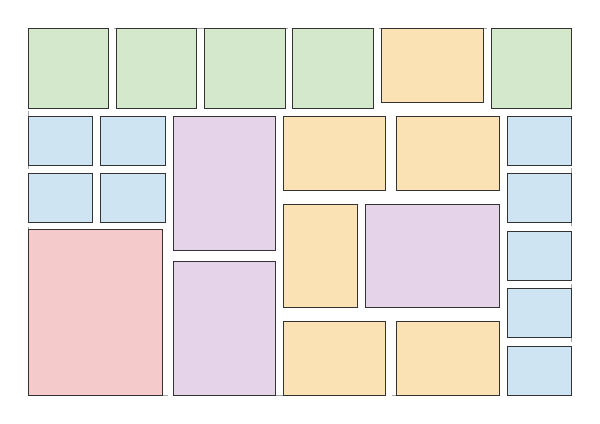
\begin{tikzpicture}[x=0.4mm, y=-0.4mm]
\draw[gray!70, dashed, line width=0.4pt] (0,0) rectangle (172.50,116.50);
\filldraw[fill=ft2, draw=black!80, line width=0.3pt] (0.00,0.00) rectangle (25.50,25.50);
\filldraw[fill=ft2, draw=black!80, line width=0.3pt] (28.00,0.00) rectangle (53.50,25.50);
\filldraw[fill=ft2, draw=black!80, line width=0.3pt] (56.00,0.00) rectangle (81.50,25.50);
\filldraw[fill=ft2, draw=black!80, line width=0.3pt] (84.00,0.00) rectangle (109.50,25.50);
\filldraw[fill=ft1, draw=black!80, line width=0.3pt] (112.00,0.00) rectangle (144.50,23.50);
\filldraw[fill=ft2, draw=black!80, line width=0.3pt] (147.00,0.00) rectangle (172.50,25.50);
\filldraw[fill=ft0, draw=black!80, line width=0.3pt] (0.00,28.00) rectangle (20.50,43.50);
\filldraw[fill=ft0, draw=black!80, line width=0.3pt] (23.00,28.00) rectangle (43.50,43.50);
\filldraw[fill=ft3, draw=black!80, line width=0.3pt] (46.00,28.00) rectangle (78.50,70.50);
\filldraw[fill=ft1, draw=black!80, line width=0.3pt] (81.00,28.00) rectangle (113.50,51.50);
\filldraw[fill=ft1, draw=black!80, line width=0.3pt] (117.00,28.00) rectangle (149.50,51.50);
\filldraw[fill=ft0, draw=black!80, line width=0.3pt] (152.00,28.00) rectangle (172.50,43.50);
\filldraw[fill=ft0, draw=black!80, line width=0.3pt] (0.00,46.00) rectangle (20.50,61.50);
\filldraw[fill=ft0, draw=black!80, line width=0.3pt] (23.00,46.00) rectangle (43.50,61.50);
\filldraw[fill=ft0, draw=black!80, line width=0.3pt] (152.00,46.25) rectangle (172.50,61.75);
\filldraw[fill=ft1, draw=black!80, line width=0.3pt] (81.00,56.00) rectangle (104.50,88.50);
\filldraw[fill=ft3, draw=black!80, line width=0.3pt] (107.00,56.00) rectangle (149.50,88.50);
\filldraw[fill=ft4, draw=black!80, line width=0.3pt] (0.00,64.00) rectangle (42.50,116.50);
\filldraw[fill=ft0, draw=black!80, line width=0.3pt] (152.00,64.50) rectangle (172.50,80.00);
\filldraw[fill=ft3, draw=black!80, line width=0.3pt] (46.00,74.00) rectangle (78.50,116.50);
\filldraw[fill=ft0, draw=black!80, line width=0.3pt] (152.00,82.75) rectangle (172.50,98.25);
\filldraw[fill=ft1, draw=black!80, line width=0.3pt] (81.00,93.00) rectangle (113.50,116.50);
\filldraw[fill=ft1, draw=black!80, line width=0.3pt] (117.00,93.00) rectangle (149.50,116.50);
\filldraw[fill=ft0, draw=black!80, line width=0.3pt] (152.00,101.00) rectangle (172.50,116.50);
\end{tikzpicture}\\[2pt]
{\small\bfseries entropy} -- \hyperref[lay:entropy:1]{layout 1}\\
{\scriptsize 172.5 $\times$ 116.5 cm, 24 frames, gap 2.5 cm,
max.\ dev.\ 2.0 cm, notches none, entropy 0.72}
\end{minipage}\hfill
\begin{minipage}[t]{0.32\textwidth}\centering\vspace{0pt}
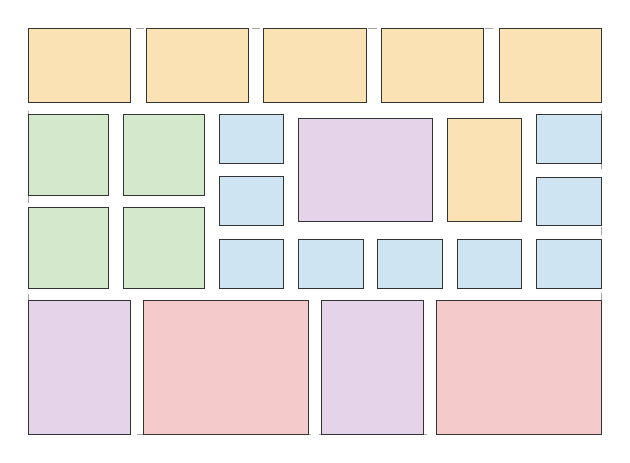
\begin{tikzpicture}[x=0.4mm, y=-0.4mm]
\draw[gray!70, dashed, line width=0.4pt] (0,0) rectangle (182.00,129.00);
\filldraw[fill=ft1, draw=black!80, line width=0.3pt] (0.00,0.00) rectangle (32.50,23.50);
\filldraw[fill=ft1, draw=black!80, line width=0.3pt] (37.38,0.00) rectangle (69.88,23.50);
\filldraw[fill=ft1, draw=black!80, line width=0.3pt] (74.75,0.00) rectangle (107.25,23.50);
\filldraw[fill=ft1, draw=black!80, line width=0.3pt] (112.12,0.00) rectangle (144.62,23.50);
\filldraw[fill=ft1, draw=black!80, line width=0.3pt] (149.50,0.00) rectangle (182.00,23.50);
\filldraw[fill=ft2, draw=black!80, line width=0.3pt] (0.00,27.50) rectangle (25.50,53.00);
\filldraw[fill=ft2, draw=black!80, line width=0.3pt] (30.30,27.50) rectangle (55.80,53.00);
\filldraw[fill=ft0, draw=black!80, line width=0.3pt] (60.60,27.50) rectangle (81.10,43.00);
\filldraw[fill=ft0, draw=black!80, line width=0.3pt] (161.50,27.50) rectangle (182.00,43.00);
\filldraw[fill=ft3, draw=black!80, line width=0.3pt] (85.90,28.75) rectangle (128.40,61.25);
\filldraw[fill=ft1, draw=black!80, line width=0.3pt] (133.20,28.75) rectangle (156.70,61.25);
\filldraw[fill=ft0, draw=black!80, line width=0.3pt] (60.60,47.00) rectangle (81.10,62.50);
\filldraw[fill=ft0, draw=black!80, line width=0.3pt] (161.50,47.25) rectangle (182.00,62.75);
\filldraw[fill=ft2, draw=black!80, line width=0.3pt] (0.00,57.00) rectangle (25.50,82.50);
\filldraw[fill=ft2, draw=black!80, line width=0.3pt] (30.30,57.00) rectangle (55.80,82.50);
\filldraw[fill=ft0, draw=black!80, line width=0.3pt] (60.60,67.00) rectangle (81.10,82.50);
\filldraw[fill=ft0, draw=black!80, line width=0.3pt] (85.80,67.00) rectangle (106.30,82.50);
\filldraw[fill=ft0, draw=black!80, line width=0.3pt] (111.00,67.00) rectangle (131.50,82.50);
\filldraw[fill=ft0, draw=black!80, line width=0.3pt] (136.20,67.00) rectangle (156.70,82.50);
\filldraw[fill=ft0, draw=black!80, line width=0.3pt] (161.50,67.00) rectangle (182.00,82.50);
\filldraw[fill=ft3, draw=black!80, line width=0.3pt] (0.00,86.50) rectangle (32.50,129.00);
\filldraw[fill=ft4, draw=black!80, line width=0.3pt] (36.50,86.50) rectangle (89.00,129.00);
\filldraw[fill=ft3, draw=black!80, line width=0.3pt] (93.00,86.50) rectangle (125.50,129.00);
\filldraw[fill=ft4, draw=black!80, line width=0.3pt] (129.50,86.50) rectangle (182.00,129.00);
\end{tikzpicture}\\[2pt]
{\small\bfseries large-entropy} -- \hyperref[lay:large-entropy:1]{layout 1}\\
{\scriptsize 182.0 $\times$ 129.0 cm, 24 frames, gap 4 cm,
max.\ dev.\ 1.8 cm, notches none, entropy 0.65}
\end{minipage}
\par\vspace{10pt}
\clearpage

\section{free-gap}\label{sec:free-gap}
Baseline. The nominal gap is an annealing variable between 1.5 and 6 cm (steps of 0.5 cm). Where a strip of frames is shorter than its neighbour, the slack is spread evenly over the gaps inside that strip. Gap deviations and border notches are penalised with a Huber shape: quadratic up to 2 cm, linear beyond, so a few large deviations are not punished out of proportion.\\[4pt]
{\small This is the baseline the other paradigms are compared with.}\\
{\small 256 runs, 20 min wall-clock budget, 542 candidate states, the 16 best distinct layouts are shown.}\\[10pt]
\begin{tabular}{@{}r l r r r r l c r@{}}
\toprule
\# & size (cm) & gap & frames & max dev & mean dev & notches & corners & entropy \\
\midrule
\hyperref[lay:free-gap:1]{1} & 181.5 $\times$ 113.5 & 1.5 & 20 & 1.0 & 0.59 & none & 4/4 & 0.71 \\
\hyperref[lay:free-gap:2]{2} & 182.0 $\times$ 129.0 & 4 & 24 & 1.8 & 0.53 & none & 4/4 & 0.64 \\
\hyperref[lay:free-gap:3]{3} & 184.0 $\times$ 115.0 & 2 & 23 & 2.0 & 0.56 & none & 4/4 & 0.76 \\
\hyperref[lay:free-gap:4]{4} & 177.5 $\times$ 113.5 & 1.5 & 21 & 2.0 & 0.51 & none & 4/4 & 0.66 \\
\hyperref[lay:free-gap:5]{5} & 181.5 $\times$ 126.5 & 2.5 & 25 & 3.0 & 0.76 & none & 4/4 & 0.79 \\
\hyperref[lay:free-gap:6]{6} & 186.5 $\times$ 115.0 & 2 & 24 & 2.2 & 0.46 & 4 cm & 4/4 & 0.76 \\
\hyperref[lay:free-gap:7]{7} & 180.5 $\times$ 128.5 & 3.5 & 24 & 3.0 & 0.61 & none & 4/4 & 0.66 \\
\hyperref[lay:free-gap:8]{8} & 169.5 $\times$ 113.5 & 1.5 & 23 & 2.5 & 0.68 & none & 4/4 & 0.76 \\
\hyperref[lay:free-gap:9]{9} & 184.0 $\times$ 115.0 & 2 & 23 & 2.2 & 0.53 & 4 cm & 4/4 & 0.68 \\
\hyperref[lay:free-gap:10]{10} & 180.0 $\times$ 117.0 & 4 & 23 & 3.0 & 0.29 & none & 4/4 & 0.58 \\
\hyperref[lay:free-gap:11]{11} & 182.5 $\times$ 112.5 & 4.5 & 22 & 3.0 & 0.64 & none & 4/4 & 0.67 \\
\hyperref[lay:free-gap:12]{12} & 170.5 $\times$ 114.5 & 2 & 22 & 3.0 & 0.81 & none & 4/4 & 0.72 \\
\hyperref[lay:free-gap:13]{13} & 177.5 $\times$ 113.5 & 1.5 & 21 & 2.0 & 0.54 & 6 cm & 4/4 & 0.68 \\
\hyperref[lay:free-gap:14]{14} & 171.0 $\times$ 120.5 & 6 & 14 & 3.0 & 0.29 & none & 4/4 & 0.81 \\
\hyperref[lay:free-gap:15]{15} & 187.5 $\times$ 130.0 & 2 & 26 & 3.5 & 0.78 & 4 cm & 4/4 & 0.83 \\
\hyperref[lay:free-gap:16]{16} & 180.0 $\times$ 114.5 & 2 & 25 & 3.0 & 0.64 & 4 cm & 4/4 & 0.66 \\
\bottomrule
\end{tabular}
\clearpage
\phantomsection\addcontentsline{toc}{subsection}{Layout 1: 181.5 \texorpdfstring{$\times$}{x} 113.5 cm, 20 frames, gap 1.5 cm, max.\ deviation 1.0 cm}
\label{lay:free-gap:1}
\begin{minipage}[t]{0.74\textwidth}\vspace{0pt}
{\LARGE\bfseries Layout 1}\hspace{1.5em}{\large 181.5 $\times$ 113.5 cm \quad gap 1.5 cm \quad 20 frames}\\[8pt]
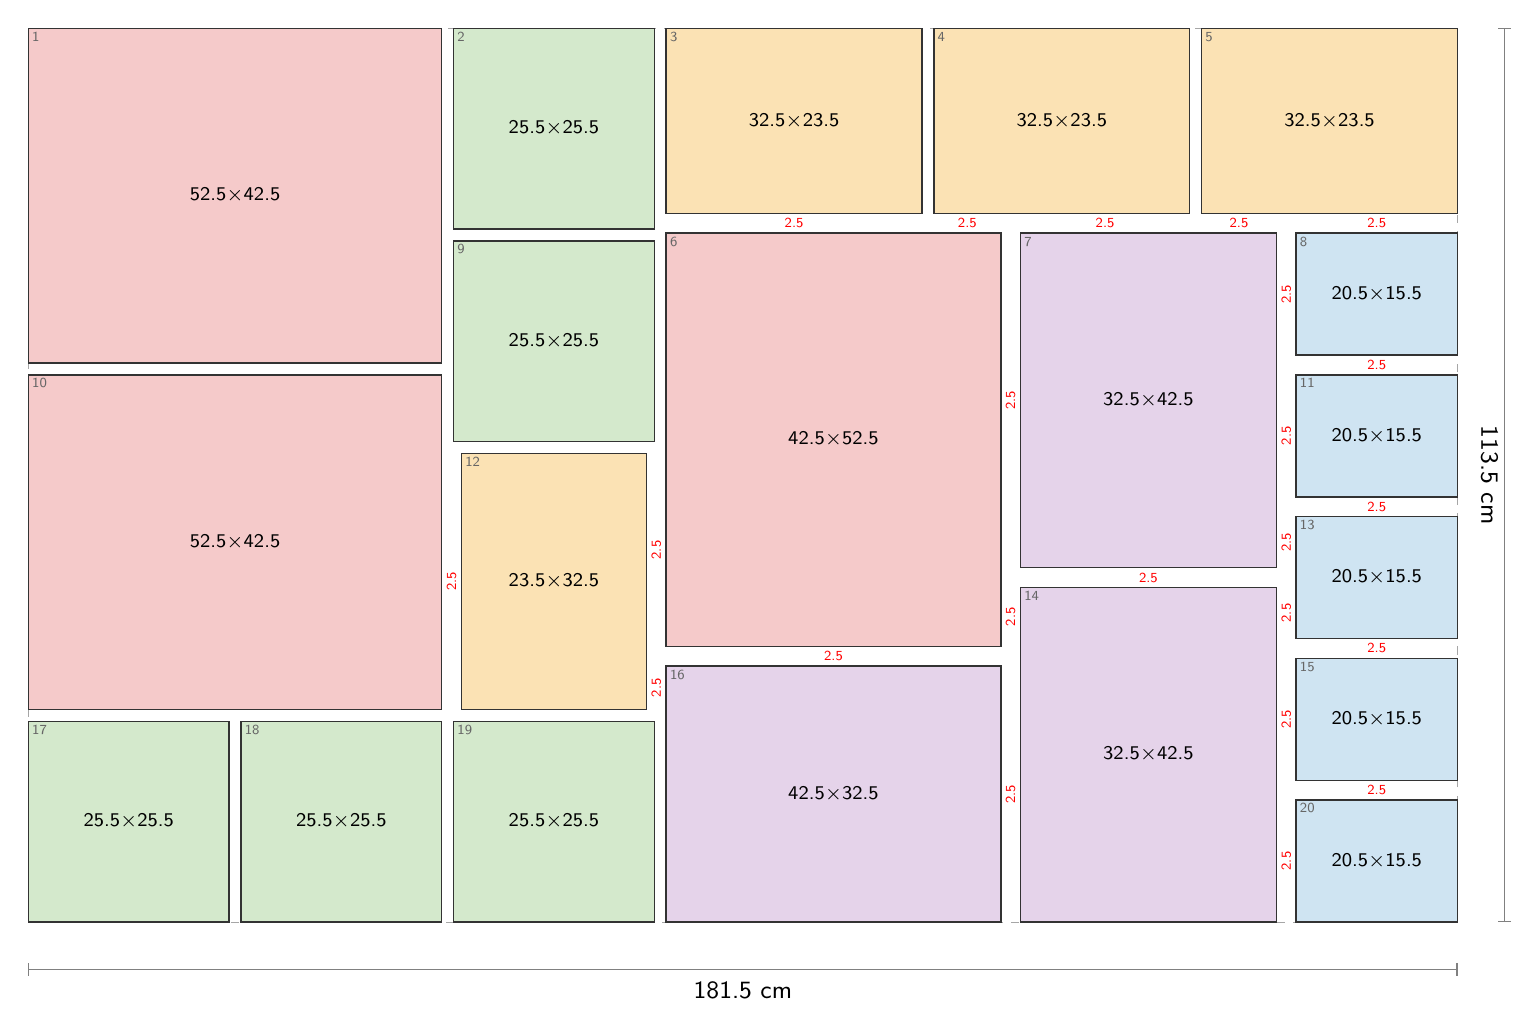
\begin{tikzpicture}[x=1mm, y=-1mm]
\draw[gray!70, dashed, line width=0.4pt] (0,0) rectangle (181.50,113.50);
\filldraw[fill=ft4, draw=black!80, line width=0.5pt] (0.00,0.00) rectangle (52.50,42.50);
\node[align=center, inner sep=0pt] at (26.25,21.25) {\scriptsize 52.5$\times$42.5};
\node[anchor=north west, inner sep=1.2pt, font=\tiny, text=black!60] at (0.00,0.00) {1};
\filldraw[fill=ft2, draw=black!80, line width=0.5pt] (54.00,0.00) rectangle (79.50,25.50);
\node[align=center, inner sep=0pt] at (66.75,12.75) {\scriptsize 25.5$\times$25.5};
\node[anchor=north west, inner sep=1.2pt, font=\tiny, text=black!60] at (54.00,0.00) {2};
\filldraw[fill=ft1, draw=black!80, line width=0.5pt] (81.00,0.00) rectangle (113.50,23.50);
\node[align=center, inner sep=0pt] at (97.25,11.75) {\scriptsize 32.5$\times$23.5};
\node[anchor=north west, inner sep=1.2pt, font=\tiny, text=black!60] at (81.00,0.00) {3};
\filldraw[fill=ft1, draw=black!80, line width=0.5pt] (115.00,0.00) rectangle (147.50,23.50);
\node[align=center, inner sep=0pt] at (131.25,11.75) {\scriptsize 32.5$\times$23.5};
\node[anchor=north west, inner sep=1.2pt, font=\tiny, text=black!60] at (115.00,0.00) {4};
\filldraw[fill=ft1, draw=black!80, line width=0.5pt] (149.00,0.00) rectangle (181.50,23.50);
\node[align=center, inner sep=0pt] at (165.25,11.75) {\scriptsize 32.5$\times$23.5};
\node[anchor=north west, inner sep=1.2pt, font=\tiny, text=black!60] at (149.00,0.00) {5};
\filldraw[fill=ft4, draw=black!80, line width=0.5pt] (81.00,26.00) rectangle (123.50,78.50);
\node[align=center, inner sep=0pt] at (102.25,52.25) {\scriptsize 42.5$\times$52.5};
\node[anchor=north west, inner sep=1.2pt, font=\tiny, text=black!60] at (81.00,26.00) {6};
\filldraw[fill=ft3, draw=black!80, line width=0.5pt] (126.00,26.00) rectangle (158.50,68.50);
\node[align=center, inner sep=0pt] at (142.25,47.25) {\scriptsize 32.5$\times$42.5};
\node[anchor=north west, inner sep=1.2pt, font=\tiny, text=black!60] at (126.00,26.00) {7};
\filldraw[fill=ft0, draw=black!80, line width=0.5pt] (161.00,26.00) rectangle (181.50,41.50);
\node[align=center, inner sep=0pt] at (171.25,33.75) {\scriptsize 20.5$\times$15.5};
\node[anchor=north west, inner sep=1.2pt, font=\tiny, text=black!60] at (161.00,26.00) {8};
\filldraw[fill=ft2, draw=black!80, line width=0.5pt] (54.00,27.00) rectangle (79.50,52.50);
\node[align=center, inner sep=0pt] at (66.75,39.75) {\scriptsize 25.5$\times$25.5};
\node[anchor=north west, inner sep=1.2pt, font=\tiny, text=black!60] at (54.00,27.00) {9};
\filldraw[fill=ft4, draw=black!80, line width=0.5pt] (0.00,44.00) rectangle (52.50,86.50);
\node[align=center, inner sep=0pt] at (26.25,65.25) {\scriptsize 52.5$\times$42.5};
\node[anchor=north west, inner sep=1.2pt, font=\tiny, text=black!60] at (0.00,44.00) {10};
\filldraw[fill=ft0, draw=black!80, line width=0.5pt] (161.00,44.00) rectangle (181.50,59.50);
\node[align=center, inner sep=0pt] at (171.25,51.75) {\scriptsize 20.5$\times$15.5};
\node[anchor=north west, inner sep=1.2pt, font=\tiny, text=black!60] at (161.00,44.00) {11};
\filldraw[fill=ft1, draw=black!80, line width=0.5pt] (55.00,54.00) rectangle (78.50,86.50);
\node[align=center, inner sep=0pt] at (66.75,70.25) {\scriptsize 23.5$\times$32.5};
\node[anchor=north west, inner sep=1.2pt, font=\tiny, text=black!60] at (55.00,54.00) {12};
\filldraw[fill=ft0, draw=black!80, line width=0.5pt] (161.00,62.00) rectangle (181.50,77.50);
\node[align=center, inner sep=0pt] at (171.25,69.75) {\scriptsize 20.5$\times$15.5};
\node[anchor=north west, inner sep=1.2pt, font=\tiny, text=black!60] at (161.00,62.00) {13};
\filldraw[fill=ft3, draw=black!80, line width=0.5pt] (126.00,71.00) rectangle (158.50,113.50);
\node[align=center, inner sep=0pt] at (142.25,92.25) {\scriptsize 32.5$\times$42.5};
\node[anchor=north west, inner sep=1.2pt, font=\tiny, text=black!60] at (126.00,71.00) {14};
\filldraw[fill=ft0, draw=black!80, line width=0.5pt] (161.00,80.00) rectangle (181.50,95.50);
\node[align=center, inner sep=0pt] at (171.25,87.75) {\scriptsize 20.5$\times$15.5};
\node[anchor=north west, inner sep=1.2pt, font=\tiny, text=black!60] at (161.00,80.00) {15};
\filldraw[fill=ft3, draw=black!80, line width=0.5pt] (81.00,81.00) rectangle (123.50,113.50);
\node[align=center, inner sep=0pt] at (102.25,97.25) {\scriptsize 42.5$\times$32.5};
\node[anchor=north west, inner sep=1.2pt, font=\tiny, text=black!60] at (81.00,81.00) {16};
\filldraw[fill=ft2, draw=black!80, line width=0.5pt] (0.00,88.00) rectangle (25.50,113.50);
\node[align=center, inner sep=0pt] at (12.75,100.75) {\scriptsize 25.5$\times$25.5};
\node[anchor=north west, inner sep=1.2pt, font=\tiny, text=black!60] at (0.00,88.00) {17};
\filldraw[fill=ft2, draw=black!80, line width=0.5pt] (27.00,88.00) rectangle (52.50,113.50);
\node[align=center, inner sep=0pt] at (39.75,100.75) {\scriptsize 25.5$\times$25.5};
\node[anchor=north west, inner sep=1.2pt, font=\tiny, text=black!60] at (27.00,88.00) {18};
\filldraw[fill=ft2, draw=black!80, line width=0.5pt] (54.00,88.00) rectangle (79.50,113.50);
\node[align=center, inner sep=0pt] at (66.75,100.75) {\scriptsize 25.5$\times$25.5};
\node[anchor=north west, inner sep=1.2pt, font=\tiny, text=black!60] at (54.00,88.00) {19};
\filldraw[fill=ft0, draw=black!80, line width=0.5pt] (161.00,98.00) rectangle (181.50,113.50);
\node[align=center, inner sep=0pt] at (171.25,105.75) {\scriptsize 20.5$\times$15.5};
\node[anchor=north west, inner sep=1.2pt, font=\tiny, text=black!60] at (161.00,98.00) {20};
\node[font=\tiny, text=red, fill=white, inner sep=0.3pt] at (97.25,24.75) {2.5};
\node[font=\tiny, text=red, fill=white, inner sep=0.3pt] at (119.25,24.75) {2.5};
\node[font=\tiny, text=red, fill=white, inner sep=0.3pt] at (136.75,24.75) {2.5};
\node[font=\tiny, text=red, fill=white, inner sep=0.3pt] at (153.75,24.75) {2.5};
\node[font=\tiny, text=red, fill=white, inner sep=0.3pt] at (171.25,24.75) {2.5};
\node[font=\tiny, text=red, fill=white, inner sep=0.3pt, rotate=90] at (124.75,47.25) {2.5};
\node[font=\tiny, text=red, fill=white, inner sep=0.3pt, rotate=90] at (124.75,74.75) {2.5};
\node[font=\tiny, text=red, fill=white, inner sep=0.3pt] at (102.25,79.75) {2.5};
\node[font=\tiny, text=red, fill=white, inner sep=0.3pt, rotate=90] at (159.75,33.75) {2.5};
\node[font=\tiny, text=red, fill=white, inner sep=0.3pt, rotate=90] at (159.75,51.75) {2.5};
\node[font=\tiny, text=red, fill=white, inner sep=0.3pt, rotate=90] at (159.75,65.25) {2.5};
\node[font=\tiny, text=red, fill=white, inner sep=0.3pt] at (142.25,69.75) {2.5};
\node[font=\tiny, text=red, fill=white, inner sep=0.3pt] at (171.25,42.75) {2.5};
\node[font=\tiny, text=red, fill=white, inner sep=0.3pt, rotate=90] at (53.75,70.25) {2.5};
\node[font=\tiny, text=red, fill=white, inner sep=0.3pt] at (171.25,60.75) {2.5};
\node[font=\tiny, text=red, fill=white, inner sep=0.3pt, rotate=90] at (79.75,66.25) {2.5};
\node[font=\tiny, text=red, fill=white, inner sep=0.3pt, rotate=90] at (79.75,83.75) {2.5};
\node[font=\tiny, text=red, fill=white, inner sep=0.3pt] at (171.25,78.75) {2.5};
\node[font=\tiny, text=red, fill=white, inner sep=0.3pt, rotate=90] at (159.75,74.25) {2.5};
\node[font=\tiny, text=red, fill=white, inner sep=0.3pt, rotate=90] at (159.75,87.75) {2.5};
\node[font=\tiny, text=red, fill=white, inner sep=0.3pt, rotate=90] at (159.75,105.75) {2.5};
\node[font=\tiny, text=red, fill=white, inner sep=0.3pt] at (171.25,96.75) {2.5};
\node[font=\tiny, text=red, fill=white, inner sep=0.3pt, rotate=90] at (124.75,97.25) {2.5};
\draw[Bar-Bar, gray] (0,119.50) -- (181.50,119.50) node[midway, below=1pt, font=\small, text=black] {181.5 cm};
\draw[Bar-Bar, gray] (187.50,0) -- (187.50,113.50) node[midway, right=1pt, font=\small, text=black, rotate=-90, anchor=north] {113.5 cm};
\end{tikzpicture}\\[4pt]
{\scriptsize Scale 1:10 (1 mm = 1 cm). Red numbers mark gaps that deviate from the nominal gap by more than 0.25 cm. Small grey numbers index the coordinate table.}
\end{minipage}\hfill
\begin{minipage}[t]{0.25\textwidth}\vspace{0pt}
\small
\begin{tabular}{@{}l l@{}}
\toprule
Outer size & 181.5 $\times$ 113.5 cm \\
Nominal gap & 1.5 cm \\
Actual gaps & 1.5 -- 2.5 cm \\
Max.\ deviation & 1.0 cm \\
Mean deviation & 0.59 cm \\
Border notches & none \\
Corners filled & 4 / 4 \\
Frames used & 20 of 28 \\
Large frames & {\scriptsize 3, touching 1$\times$ (52 cm), min.\ dist.\ 44 cm} \\
Entropy & 0.71 \\
\quad {\scriptsize mix / variety} & {\scriptsize 0.86 / 0.72} \\
\quad {\scriptsize stagger / lines} & {\scriptsize 0.51 / 0.75 (2 through)} \\
\bottomrule
\end{tabular}

\vspace{8pt}
\scriptsize
\begin{tabular}{@{}c l l r r@{}}
\toprule
 & outer w $\times$ h (cm) &  & used & have \\
\midrule
\tikz[baseline=-0.6ex]\fill[ft0,draw=black!60] (0,0) rectangle (1.2ex,1.2ex); & 20.5$\times$15.5 & L & 5 & 9 \\
\tikz[baseline=-0.6ex]\fill[ft0,draw=black!60] (0,0) rectangle (1.2ex,1.2ex); & 15.5$\times$20.5 & P & 0 & 2 \\
\tikz[baseline=-0.6ex]\fill[ft3,draw=black!60] (0,0) rectangle (1.2ex,1.2ex); & 32.5$\times$42.5 & P & 2 & 2 \\
\tikz[baseline=-0.6ex]\fill[ft3,draw=black!60] (0,0) rectangle (1.2ex,1.2ex); & 42.5$\times$32.5 & L & 1 & 1 \\
\tikz[baseline=-0.6ex]\fill[ft1,draw=black!60] (0,0) rectangle (1.2ex,1.2ex); & 32.5$\times$23.5 & L & 3 & 5 \\
\tikz[baseline=-0.6ex]\fill[ft1,draw=black!60] (0,0) rectangle (1.2ex,1.2ex); & 23.5$\times$32.5 & P & 1 & 1 \\
\tikz[baseline=-0.6ex]\fill[ft2,draw=black!60] (0,0) rectangle (1.2ex,1.2ex); & 25.5$\times$25.5 &  & 5 & 5 \\
\tikz[baseline=-0.6ex]\fill[ft4,draw=black!60] (0,0) rectangle (1.2ex,1.2ex); & 42.5$\times$52.5 & P & 1 & 1 \\
\tikz[baseline=-0.6ex]\fill[ft4,draw=black!60] (0,0) rectangle (1.2ex,1.2ex); & 52.5$\times$42.5 & L & 2 & 2 \\
\bottomrule
\end{tabular}

\vspace{8pt}
{\bfseries Positions} (top-left corner, cm)\\[2pt]
\tiny
\begin{tabular}{@{}r l r r@{}}
\toprule
\# & frame w $\times$ h & x & y \\
\midrule
1 & 52.5 $\times$ 42.5 & 0.0 & 0.0 \\
2 & 25.5 $\times$ 25.5 & 54.0 & 0.0 \\
3 & 32.5 $\times$ 23.5 & 81.0 & 0.0 \\
4 & 32.5 $\times$ 23.5 & 115.0 & 0.0 \\
5 & 32.5 $\times$ 23.5 & 149.0 & 0.0 \\
6 & 42.5 $\times$ 52.5 & 81.0 & 26.0 \\
7 & 32.5 $\times$ 42.5 & 126.0 & 26.0 \\
8 & 20.5 $\times$ 15.5 & 161.0 & 26.0 \\
9 & 25.5 $\times$ 25.5 & 54.0 & 27.0 \\
10 & 52.5 $\times$ 42.5 & 0.0 & 44.0 \\
11 & 20.5 $\times$ 15.5 & 161.0 & 44.0 \\
12 & 23.5 $\times$ 32.5 & 55.0 & 54.0 \\
13 & 20.5 $\times$ 15.5 & 161.0 & 62.0 \\
14 & 32.5 $\times$ 42.5 & 126.0 & 71.0 \\
15 & 20.5 $\times$ 15.5 & 161.0 & 80.0 \\
16 & 42.5 $\times$ 32.5 & 81.0 & 81.0 \\
17 & 25.5 $\times$ 25.5 & 0.0 & 88.0 \\
18 & 25.5 $\times$ 25.5 & 27.0 & 88.0 \\
19 & 25.5 $\times$ 25.5 & 54.0 & 88.0 \\
20 & 20.5 $\times$ 15.5 & 161.0 & 98.0 \\
\bottomrule
\end{tabular}
\end{minipage}
\clearpage

\phantomsection\addcontentsline{toc}{subsection}{Layout 2: 182.0 \texorpdfstring{$\times$}{x} 129.0 cm, 24 frames, gap 4 cm, max.\ deviation 1.8 cm}
\label{lay:free-gap:2}
\begin{minipage}[t]{0.74\textwidth}\vspace{0pt}
{\LARGE\bfseries Layout 2}\hspace{1.5em}{\large 182.0 $\times$ 129.0 cm \quad gap 4 cm \quad 24 frames}\\[8pt]
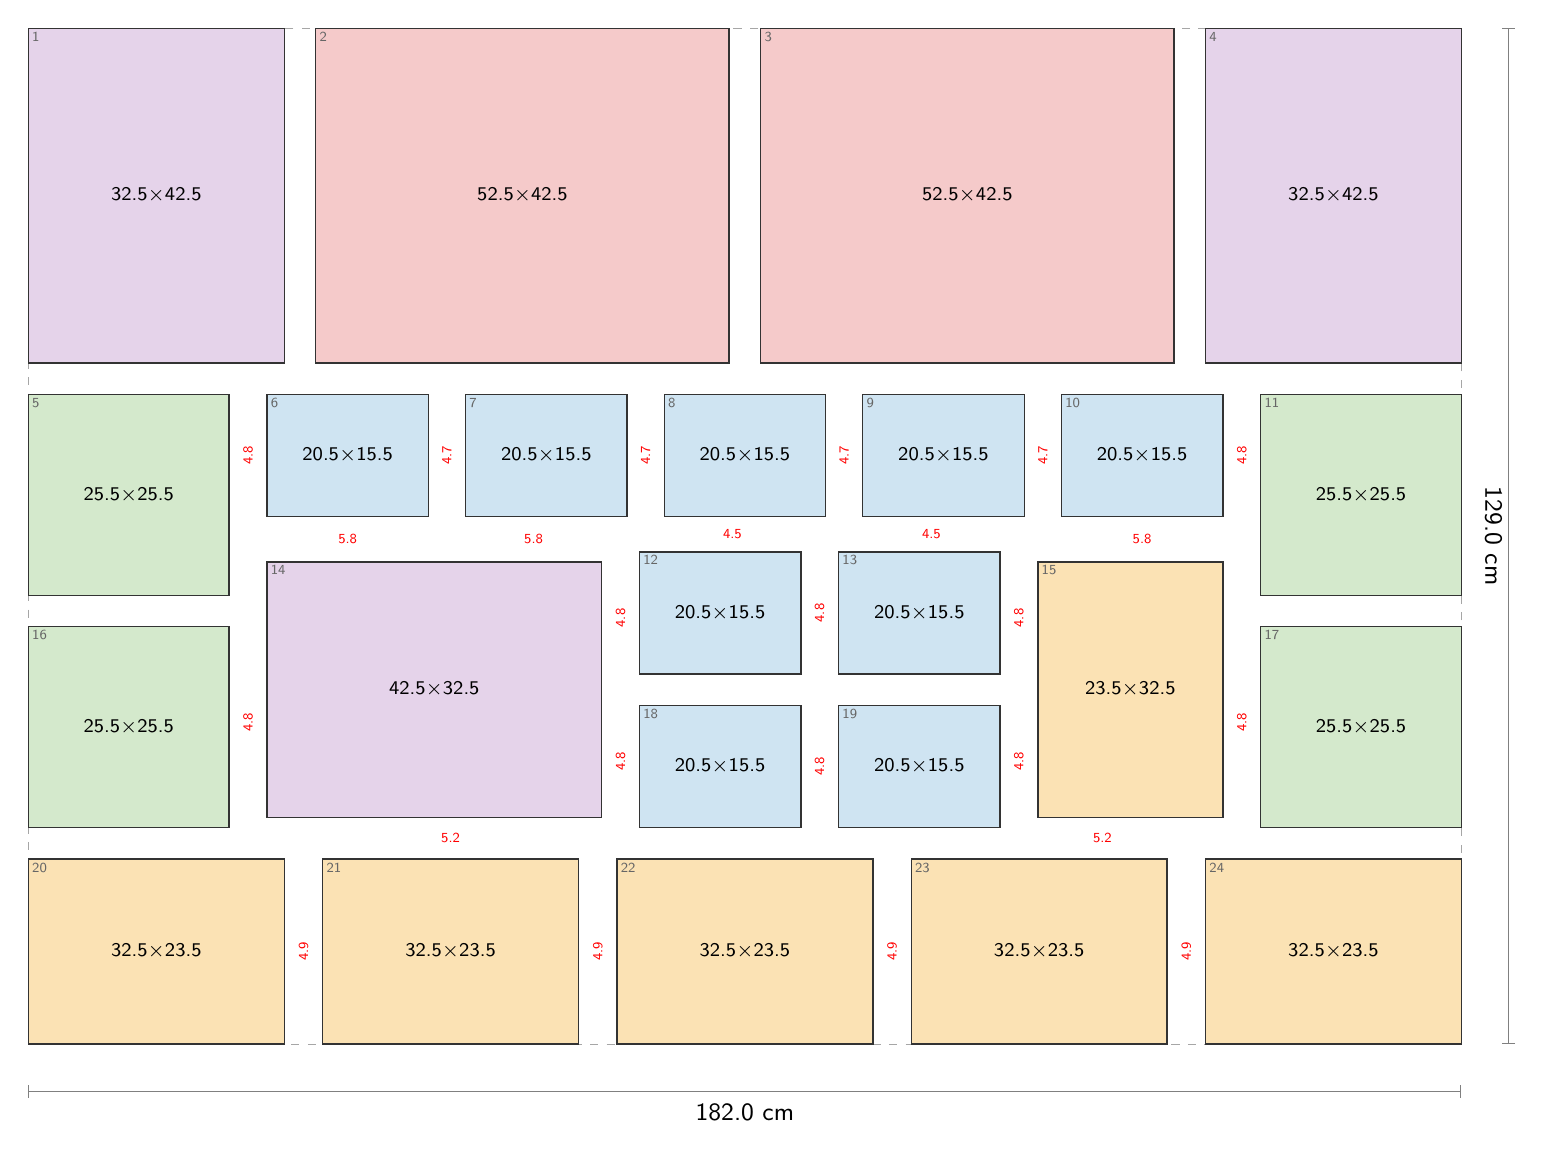
\begin{tikzpicture}[x=1mm, y=-1mm]
\draw[gray!70, dashed, line width=0.4pt] (0,0) rectangle (182.00,129.00);
\filldraw[fill=ft3, draw=black!80, line width=0.5pt] (0.00,0.00) rectangle (32.50,42.50);
\node[align=center, inner sep=0pt] at (16.25,21.25) {\scriptsize 32.5$\times$42.5};
\node[anchor=north west, inner sep=1.2pt, font=\tiny, text=black!60] at (0.00,0.00) {1};
\filldraw[fill=ft4, draw=black!80, line width=0.5pt] (36.50,0.00) rectangle (89.00,42.50);
\node[align=center, inner sep=0pt] at (62.75,21.25) {\scriptsize 52.5$\times$42.5};
\node[anchor=north west, inner sep=1.2pt, font=\tiny, text=black!60] at (36.50,0.00) {2};
\filldraw[fill=ft4, draw=black!80, line width=0.5pt] (93.00,0.00) rectangle (145.50,42.50);
\node[align=center, inner sep=0pt] at (119.25,21.25) {\scriptsize 52.5$\times$42.5};
\node[anchor=north west, inner sep=1.2pt, font=\tiny, text=black!60] at (93.00,0.00) {3};
\filldraw[fill=ft3, draw=black!80, line width=0.5pt] (149.50,0.00) rectangle (182.00,42.50);
\node[align=center, inner sep=0pt] at (165.75,21.25) {\scriptsize 32.5$\times$42.5};
\node[anchor=north west, inner sep=1.2pt, font=\tiny, text=black!60] at (149.50,0.00) {4};
\filldraw[fill=ft2, draw=black!80, line width=0.5pt] (0.00,46.50) rectangle (25.50,72.00);
\node[align=center, inner sep=0pt] at (12.75,59.25) {\scriptsize 25.5$\times$25.5};
\node[anchor=north west, inner sep=1.2pt, font=\tiny, text=black!60] at (0.00,46.50) {5};
\filldraw[fill=ft0, draw=black!80, line width=0.5pt] (30.30,46.50) rectangle (50.80,62.00);
\node[align=center, inner sep=0pt] at (40.55,54.25) {\scriptsize 20.5$\times$15.5};
\node[anchor=north west, inner sep=1.2pt, font=\tiny, text=black!60] at (30.30,46.50) {6};
\filldraw[fill=ft0, draw=black!80, line width=0.5pt] (55.52,46.50) rectangle (76.03,62.00);
\node[align=center, inner sep=0pt] at (65.78,54.25) {\scriptsize 20.5$\times$15.5};
\node[anchor=north west, inner sep=1.2pt, font=\tiny, text=black!60] at (55.52,46.50) {7};
\filldraw[fill=ft0, draw=black!80, line width=0.5pt] (80.75,46.50) rectangle (101.25,62.00);
\node[align=center, inner sep=0pt] at (91.00,54.25) {\scriptsize 20.5$\times$15.5};
\node[anchor=north west, inner sep=1.2pt, font=\tiny, text=black!60] at (80.75,46.50) {8};
\filldraw[fill=ft0, draw=black!80, line width=0.5pt] (105.97,46.50) rectangle (126.47,62.00);
\node[align=center, inner sep=0pt] at (116.22,54.25) {\scriptsize 20.5$\times$15.5};
\node[anchor=north west, inner sep=1.2pt, font=\tiny, text=black!60] at (105.97,46.50) {9};
\filldraw[fill=ft0, draw=black!80, line width=0.5pt] (131.20,46.50) rectangle (151.70,62.00);
\node[align=center, inner sep=0pt] at (141.45,54.25) {\scriptsize 20.5$\times$15.5};
\node[anchor=north west, inner sep=1.2pt, font=\tiny, text=black!60] at (131.20,46.50) {10};
\filldraw[fill=ft2, draw=black!80, line width=0.5pt] (156.50,46.50) rectangle (182.00,72.00);
\node[align=center, inner sep=0pt] at (169.25,59.25) {\scriptsize 25.5$\times$25.5};
\node[anchor=north west, inner sep=1.2pt, font=\tiny, text=black!60] at (156.50,46.50) {11};
\filldraw[fill=ft0, draw=black!80, line width=0.5pt] (77.60,66.50) rectangle (98.10,82.00);
\node[align=center, inner sep=0pt] at (87.85,74.25) {\scriptsize 20.5$\times$15.5};
\node[anchor=north west, inner sep=1.2pt, font=\tiny, text=black!60] at (77.60,66.50) {12};
\filldraw[fill=ft0, draw=black!80, line width=0.5pt] (102.90,66.50) rectangle (123.40,82.00);
\node[align=center, inner sep=0pt] at (113.15,74.25) {\scriptsize 20.5$\times$15.5};
\node[anchor=north west, inner sep=1.2pt, font=\tiny, text=black!60] at (102.90,66.50) {13};
\filldraw[fill=ft3, draw=black!80, line width=0.5pt] (30.30,67.75) rectangle (72.80,100.25);
\node[align=center, inner sep=0pt] at (51.55,84.00) {\scriptsize 42.5$\times$32.5};
\node[anchor=north west, inner sep=1.2pt, font=\tiny, text=black!60] at (30.30,67.75) {14};
\filldraw[fill=ft1, draw=black!80, line width=0.5pt] (128.20,67.75) rectangle (151.70,100.25);
\node[align=center, inner sep=0pt] at (139.95,84.00) {\scriptsize 23.5$\times$32.5};
\node[anchor=north west, inner sep=1.2pt, font=\tiny, text=black!60] at (128.20,67.75) {15};
\filldraw[fill=ft2, draw=black!80, line width=0.5pt] (0.00,76.00) rectangle (25.50,101.50);
\node[align=center, inner sep=0pt] at (12.75,88.75) {\scriptsize 25.5$\times$25.5};
\node[anchor=north west, inner sep=1.2pt, font=\tiny, text=black!60] at (0.00,76.00) {16};
\filldraw[fill=ft2, draw=black!80, line width=0.5pt] (156.50,76.00) rectangle (182.00,101.50);
\node[align=center, inner sep=0pt] at (169.25,88.75) {\scriptsize 25.5$\times$25.5};
\node[anchor=north west, inner sep=1.2pt, font=\tiny, text=black!60] at (156.50,76.00) {17};
\filldraw[fill=ft0, draw=black!80, line width=0.5pt] (77.60,86.00) rectangle (98.10,101.50);
\node[align=center, inner sep=0pt] at (87.85,93.75) {\scriptsize 20.5$\times$15.5};
\node[anchor=north west, inner sep=1.2pt, font=\tiny, text=black!60] at (77.60,86.00) {18};
\filldraw[fill=ft0, draw=black!80, line width=0.5pt] (102.90,86.00) rectangle (123.40,101.50);
\node[align=center, inner sep=0pt] at (113.15,93.75) {\scriptsize 20.5$\times$15.5};
\node[anchor=north west, inner sep=1.2pt, font=\tiny, text=black!60] at (102.90,86.00) {19};
\filldraw[fill=ft1, draw=black!80, line width=0.5pt] (0.00,105.50) rectangle (32.50,129.00);
\node[align=center, inner sep=0pt] at (16.25,117.25) {\scriptsize 32.5$\times$23.5};
\node[anchor=north west, inner sep=1.2pt, font=\tiny, text=black!60] at (0.00,105.50) {20};
\filldraw[fill=ft1, draw=black!80, line width=0.5pt] (37.38,105.50) rectangle (69.88,129.00);
\node[align=center, inner sep=0pt] at (53.62,117.25) {\scriptsize 32.5$\times$23.5};
\node[anchor=north west, inner sep=1.2pt, font=\tiny, text=black!60] at (37.38,105.50) {21};
\filldraw[fill=ft1, draw=black!80, line width=0.5pt] (74.75,105.50) rectangle (107.25,129.00);
\node[align=center, inner sep=0pt] at (91.00,117.25) {\scriptsize 32.5$\times$23.5};
\node[anchor=north west, inner sep=1.2pt, font=\tiny, text=black!60] at (74.75,105.50) {22};
\filldraw[fill=ft1, draw=black!80, line width=0.5pt] (112.12,105.50) rectangle (144.62,129.00);
\node[align=center, inner sep=0pt] at (128.38,117.25) {\scriptsize 32.5$\times$23.5};
\node[anchor=north west, inner sep=1.2pt, font=\tiny, text=black!60] at (112.12,105.50) {23};
\filldraw[fill=ft1, draw=black!80, line width=0.5pt] (149.50,105.50) rectangle (182.00,129.00);
\node[align=center, inner sep=0pt] at (165.75,117.25) {\scriptsize 32.5$\times$23.5};
\node[anchor=north west, inner sep=1.2pt, font=\tiny, text=black!60] at (149.50,105.50) {24};
\node[font=\tiny, text=red, fill=white, inner sep=0.3pt, rotate=90] at (27.90,54.25) {4.8};
\node[font=\tiny, text=red, fill=white, inner sep=0.3pt, rotate=90] at (53.16,54.25) {4.7};
\node[font=\tiny, text=red, fill=white, inner sep=0.3pt] at (40.55,64.88) {5.8};
\node[font=\tiny, text=red, fill=white, inner sep=0.3pt, rotate=90] at (78.39,54.25) {4.7};
\node[font=\tiny, text=red, fill=white, inner sep=0.3pt] at (64.16,64.88) {5.8};
\node[font=\tiny, text=red, fill=white, inner sep=0.3pt, rotate=90] at (103.61,54.25) {4.7};
\node[font=\tiny, text=red, fill=white, inner sep=0.3pt] at (89.42,64.25) {4.5};
\node[font=\tiny, text=red, fill=white, inner sep=0.3pt, rotate=90] at (128.84,54.25) {4.7};
\node[font=\tiny, text=red, fill=white, inner sep=0.3pt] at (114.69,64.25) {4.5};
\node[font=\tiny, text=red, fill=white, inner sep=0.3pt, rotate=90] at (154.10,54.25) {4.8};
\node[font=\tiny, text=red, fill=white, inner sep=0.3pt] at (141.45,64.88) {5.8};
\node[font=\tiny, text=red, fill=white, inner sep=0.3pt, rotate=90] at (100.50,74.25) {4.8};
\node[font=\tiny, text=red, fill=white, inner sep=0.3pt, rotate=90] at (125.80,74.88) {4.8};
\node[font=\tiny, text=red, fill=white, inner sep=0.3pt, rotate=90] at (75.20,74.88) {4.8};
\node[font=\tiny, text=red, fill=white, inner sep=0.3pt, rotate=90] at (75.20,93.12) {4.8};
\node[font=\tiny, text=red, fill=white, inner sep=0.3pt] at (53.62,102.88) {5.2};
\node[font=\tiny, text=red, fill=white, inner sep=0.3pt, rotate=90] at (154.10,88.12) {4.8};
\node[font=\tiny, text=red, fill=white, inner sep=0.3pt] at (136.41,102.88) {5.2};
\node[font=\tiny, text=red, fill=white, inner sep=0.3pt, rotate=90] at (27.90,88.12) {4.8};
\node[font=\tiny, text=red, fill=white, inner sep=0.3pt, rotate=90] at (100.50,93.75) {4.8};
\node[font=\tiny, text=red, fill=white, inner sep=0.3pt, rotate=90] at (125.80,93.12) {4.8};
\node[font=\tiny, text=red, fill=white, inner sep=0.3pt, rotate=90] at (34.94,117.25) {4.9};
\node[font=\tiny, text=red, fill=white, inner sep=0.3pt, rotate=90] at (72.31,117.25) {4.9};
\node[font=\tiny, text=red, fill=white, inner sep=0.3pt, rotate=90] at (109.69,117.25) {4.9};
\node[font=\tiny, text=red, fill=white, inner sep=0.3pt, rotate=90] at (147.06,117.25) {4.9};
\draw[Bar-Bar, gray] (0,135.00) -- (182.00,135.00) node[midway, below=1pt, font=\small, text=black] {182.0 cm};
\draw[Bar-Bar, gray] (188.00,0) -- (188.00,129.00) node[midway, right=1pt, font=\small, text=black, rotate=-90, anchor=north] {129.0 cm};
\end{tikzpicture}\\[4pt]
{\scriptsize Scale 1:10 (1 mm = 1 cm). Red numbers mark gaps that deviate from the nominal gap by more than 0.25 cm. Small grey numbers index the coordinate table.}
\end{minipage}\hfill
\begin{minipage}[t]{0.25\textwidth}\vspace{0pt}
\small
\begin{tabular}{@{}l l@{}}
\toprule
Outer size & 182.0 $\times$ 129.0 cm \\
Nominal gap & 4 cm \\
Actual gaps & 4.0 -- 5.8 cm \\
Max.\ deviation & 1.8 cm \\
Mean deviation & 0.53 cm \\
Border notches & none \\
Corners filled & 4 / 4 \\
Frames used & 24 of 28 \\
Large frames & {\scriptsize 2, touching 1$\times$ (42 cm), min.\ dist.\ 56 cm} \\
Entropy & 0.64 \\
\quad {\scriptsize mix / variety} & {\scriptsize 0.76 / 0.56} \\
\quad {\scriptsize stagger / lines} & {\scriptsize 0.48 / 0.75 (2 through)} \\
\bottomrule
\end{tabular}

\vspace{8pt}
\scriptsize
\begin{tabular}{@{}c l l r r@{}}
\toprule
 & outer w $\times$ h (cm) &  & used & have \\
\midrule
\tikz[baseline=-0.6ex]\fill[ft0,draw=black!60] (0,0) rectangle (1.2ex,1.2ex); & 20.5$\times$15.5 & L & 9 & 9 \\
\tikz[baseline=-0.6ex]\fill[ft0,draw=black!60] (0,0) rectangle (1.2ex,1.2ex); & 15.5$\times$20.5 & P & 0 & 2 \\
\tikz[baseline=-0.6ex]\fill[ft3,draw=black!60] (0,0) rectangle (1.2ex,1.2ex); & 32.5$\times$42.5 & P & 2 & 2 \\
\tikz[baseline=-0.6ex]\fill[ft3,draw=black!60] (0,0) rectangle (1.2ex,1.2ex); & 42.5$\times$32.5 & L & 1 & 1 \\
\tikz[baseline=-0.6ex]\fill[ft1,draw=black!60] (0,0) rectangle (1.2ex,1.2ex); & 32.5$\times$23.5 & L & 5 & 5 \\
\tikz[baseline=-0.6ex]\fill[ft1,draw=black!60] (0,0) rectangle (1.2ex,1.2ex); & 23.5$\times$32.5 & P & 1 & 1 \\
\tikz[baseline=-0.6ex]\fill[ft2,draw=black!60] (0,0) rectangle (1.2ex,1.2ex); & 25.5$\times$25.5 &  & 4 & 5 \\
\tikz[baseline=-0.6ex]\fill[ft4,draw=black!60] (0,0) rectangle (1.2ex,1.2ex); & 42.5$\times$52.5 & P & 0 & 1 \\
\tikz[baseline=-0.6ex]\fill[ft4,draw=black!60] (0,0) rectangle (1.2ex,1.2ex); & 52.5$\times$42.5 & L & 2 & 2 \\
\bottomrule
\end{tabular}

\vspace{8pt}
{\bfseries Positions} (top-left corner, cm)\\[2pt]
\tiny
\begin{tabular}{@{}r l r r@{}}
\toprule
\# & frame w $\times$ h & x & y \\
\midrule
1 & 32.5 $\times$ 42.5 & 0.0 & 0.0 \\
2 & 52.5 $\times$ 42.5 & 36.5 & 0.0 \\
3 & 52.5 $\times$ 42.5 & 93.0 & 0.0 \\
4 & 32.5 $\times$ 42.5 & 149.5 & 0.0 \\
5 & 25.5 $\times$ 25.5 & 0.0 & 46.5 \\
6 & 20.5 $\times$ 15.5 & 30.3 & 46.5 \\
7 & 20.5 $\times$ 15.5 & 55.5 & 46.5 \\
8 & 20.5 $\times$ 15.5 & 80.8 & 46.5 \\
9 & 20.5 $\times$ 15.5 & 106.0 & 46.5 \\
10 & 20.5 $\times$ 15.5 & 131.2 & 46.5 \\
11 & 25.5 $\times$ 25.5 & 156.5 & 46.5 \\
12 & 20.5 $\times$ 15.5 & 77.6 & 66.5 \\
13 & 20.5 $\times$ 15.5 & 102.9 & 66.5 \\
14 & 42.5 $\times$ 32.5 & 30.3 & 67.8 \\
15 & 23.5 $\times$ 32.5 & 128.2 & 67.8 \\
16 & 25.5 $\times$ 25.5 & 0.0 & 76.0 \\
17 & 25.5 $\times$ 25.5 & 156.5 & 76.0 \\
18 & 20.5 $\times$ 15.5 & 77.6 & 86.0 \\
19 & 20.5 $\times$ 15.5 & 102.9 & 86.0 \\
20 & 32.5 $\times$ 23.5 & 0.0 & 105.5 \\
21 & 32.5 $\times$ 23.5 & 37.4 & 105.5 \\
22 & 32.5 $\times$ 23.5 & 74.8 & 105.5 \\
23 & 32.5 $\times$ 23.5 & 112.1 & 105.5 \\
24 & 32.5 $\times$ 23.5 & 149.5 & 105.5 \\
\bottomrule
\end{tabular}
\end{minipage}
\clearpage

\phantomsection\addcontentsline{toc}{subsection}{Layout 3: 184.0 \texorpdfstring{$\times$}{x} 115.0 cm, 23 frames, gap 2 cm, max.\ deviation 2.0 cm}
\label{lay:free-gap:3}
\begin{minipage}[t]{0.74\textwidth}\vspace{0pt}
{\LARGE\bfseries Layout 3}\hspace{1.5em}{\large 184.0 $\times$ 115.0 cm \quad gap 2 cm \quad 23 frames}\\[8pt]
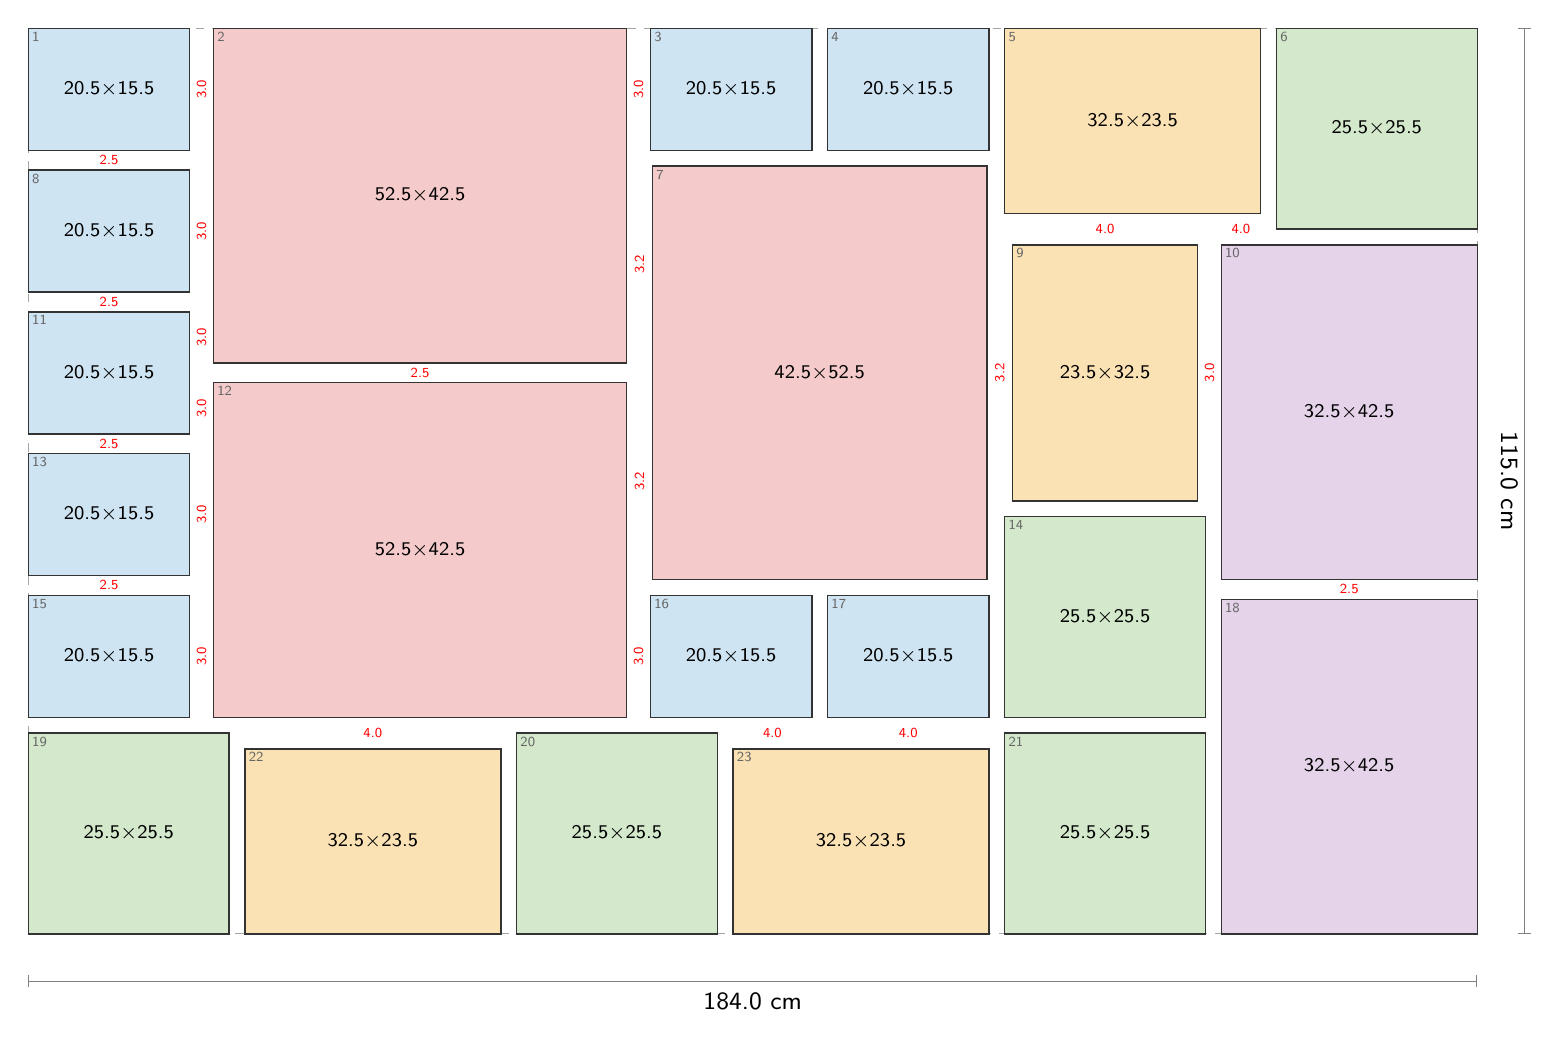
\begin{tikzpicture}[x=1mm, y=-1mm]
\draw[gray!70, dashed, line width=0.4pt] (0,0) rectangle (184.00,115.00);
\filldraw[fill=ft0, draw=black!80, line width=0.5pt] (0.00,0.00) rectangle (20.50,15.50);
\node[align=center, inner sep=0pt] at (10.25,7.75) {\scriptsize 20.5$\times$15.5};
\node[anchor=north west, inner sep=1.2pt, font=\tiny, text=black!60] at (0.00,0.00) {1};
\filldraw[fill=ft4, draw=black!80, line width=0.5pt] (23.50,0.00) rectangle (76.00,42.50);
\node[align=center, inner sep=0pt] at (49.75,21.25) {\scriptsize 52.5$\times$42.5};
\node[anchor=north west, inner sep=1.2pt, font=\tiny, text=black!60] at (23.50,0.00) {2};
\filldraw[fill=ft0, draw=black!80, line width=0.5pt] (79.00,0.00) rectangle (99.50,15.50);
\node[align=center, inner sep=0pt] at (89.25,7.75) {\scriptsize 20.5$\times$15.5};
\node[anchor=north west, inner sep=1.2pt, font=\tiny, text=black!60] at (79.00,0.00) {3};
\filldraw[fill=ft0, draw=black!80, line width=0.5pt] (101.50,0.00) rectangle (122.00,15.50);
\node[align=center, inner sep=0pt] at (111.75,7.75) {\scriptsize 20.5$\times$15.5};
\node[anchor=north west, inner sep=1.2pt, font=\tiny, text=black!60] at (101.50,0.00) {4};
\filldraw[fill=ft1, draw=black!80, line width=0.5pt] (124.00,0.00) rectangle (156.50,23.50);
\node[align=center, inner sep=0pt] at (140.25,11.75) {\scriptsize 32.5$\times$23.5};
\node[anchor=north west, inner sep=1.2pt, font=\tiny, text=black!60] at (124.00,0.00) {5};
\filldraw[fill=ft2, draw=black!80, line width=0.5pt] (158.50,0.00) rectangle (184.00,25.50);
\node[align=center, inner sep=0pt] at (171.25,12.75) {\scriptsize 25.5$\times$25.5};
\node[anchor=north west, inner sep=1.2pt, font=\tiny, text=black!60] at (158.50,0.00) {6};
\filldraw[fill=ft4, draw=black!80, line width=0.5pt] (79.25,17.50) rectangle (121.75,70.00);
\node[align=center, inner sep=0pt] at (100.50,43.75) {\scriptsize 42.5$\times$52.5};
\node[anchor=north west, inner sep=1.2pt, font=\tiny, text=black!60] at (79.25,17.50) {7};
\filldraw[fill=ft0, draw=black!80, line width=0.5pt] (0.00,18.00) rectangle (20.50,33.50);
\node[align=center, inner sep=0pt] at (10.25,25.75) {\scriptsize 20.5$\times$15.5};
\node[anchor=north west, inner sep=1.2pt, font=\tiny, text=black!60] at (0.00,18.00) {8};
\filldraw[fill=ft1, draw=black!80, line width=0.5pt] (125.00,27.50) rectangle (148.50,60.00);
\node[align=center, inner sep=0pt] at (136.75,43.75) {\scriptsize 23.5$\times$32.5};
\node[anchor=north west, inner sep=1.2pt, font=\tiny, text=black!60] at (125.00,27.50) {9};
\filldraw[fill=ft3, draw=black!80, line width=0.5pt] (151.50,27.50) rectangle (184.00,70.00);
\node[align=center, inner sep=0pt] at (167.75,48.75) {\scriptsize 32.5$\times$42.5};
\node[anchor=north west, inner sep=1.2pt, font=\tiny, text=black!60] at (151.50,27.50) {10};
\filldraw[fill=ft0, draw=black!80, line width=0.5pt] (0.00,36.00) rectangle (20.50,51.50);
\node[align=center, inner sep=0pt] at (10.25,43.75) {\scriptsize 20.5$\times$15.5};
\node[anchor=north west, inner sep=1.2pt, font=\tiny, text=black!60] at (0.00,36.00) {11};
\filldraw[fill=ft4, draw=black!80, line width=0.5pt] (23.50,45.00) rectangle (76.00,87.50);
\node[align=center, inner sep=0pt] at (49.75,66.25) {\scriptsize 52.5$\times$42.5};
\node[anchor=north west, inner sep=1.2pt, font=\tiny, text=black!60] at (23.50,45.00) {12};
\filldraw[fill=ft0, draw=black!80, line width=0.5pt] (0.00,54.00) rectangle (20.50,69.50);
\node[align=center, inner sep=0pt] at (10.25,61.75) {\scriptsize 20.5$\times$15.5};
\node[anchor=north west, inner sep=1.2pt, font=\tiny, text=black!60] at (0.00,54.00) {13};
\filldraw[fill=ft2, draw=black!80, line width=0.5pt] (124.00,62.00) rectangle (149.50,87.50);
\node[align=center, inner sep=0pt] at (136.75,74.75) {\scriptsize 25.5$\times$25.5};
\node[anchor=north west, inner sep=1.2pt, font=\tiny, text=black!60] at (124.00,62.00) {14};
\filldraw[fill=ft0, draw=black!80, line width=0.5pt] (0.00,72.00) rectangle (20.50,87.50);
\node[align=center, inner sep=0pt] at (10.25,79.75) {\scriptsize 20.5$\times$15.5};
\node[anchor=north west, inner sep=1.2pt, font=\tiny, text=black!60] at (0.00,72.00) {15};
\filldraw[fill=ft0, draw=black!80, line width=0.5pt] (79.00,72.00) rectangle (99.50,87.50);
\node[align=center, inner sep=0pt] at (89.25,79.75) {\scriptsize 20.5$\times$15.5};
\node[anchor=north west, inner sep=1.2pt, font=\tiny, text=black!60] at (79.00,72.00) {16};
\filldraw[fill=ft0, draw=black!80, line width=0.5pt] (101.50,72.00) rectangle (122.00,87.50);
\node[align=center, inner sep=0pt] at (111.75,79.75) {\scriptsize 20.5$\times$15.5};
\node[anchor=north west, inner sep=1.2pt, font=\tiny, text=black!60] at (101.50,72.00) {17};
\filldraw[fill=ft3, draw=black!80, line width=0.5pt] (151.50,72.50) rectangle (184.00,115.00);
\node[align=center, inner sep=0pt] at (167.75,93.75) {\scriptsize 32.5$\times$42.5};
\node[anchor=north west, inner sep=1.2pt, font=\tiny, text=black!60] at (151.50,72.50) {18};
\filldraw[fill=ft2, draw=black!80, line width=0.5pt] (0.00,89.50) rectangle (25.50,115.00);
\node[align=center, inner sep=0pt] at (12.75,102.25) {\scriptsize 25.5$\times$25.5};
\node[anchor=north west, inner sep=1.2pt, font=\tiny, text=black!60] at (0.00,89.50) {19};
\filldraw[fill=ft2, draw=black!80, line width=0.5pt] (62.00,89.50) rectangle (87.50,115.00);
\node[align=center, inner sep=0pt] at (74.75,102.25) {\scriptsize 25.5$\times$25.5};
\node[anchor=north west, inner sep=1.2pt, font=\tiny, text=black!60] at (62.00,89.50) {20};
\filldraw[fill=ft2, draw=black!80, line width=0.5pt] (124.00,89.50) rectangle (149.50,115.00);
\node[align=center, inner sep=0pt] at (136.75,102.25) {\scriptsize 25.5$\times$25.5};
\node[anchor=north west, inner sep=1.2pt, font=\tiny, text=black!60] at (124.00,89.50) {21};
\filldraw[fill=ft1, draw=black!80, line width=0.5pt] (27.50,91.50) rectangle (60.00,115.00);
\node[align=center, inner sep=0pt] at (43.75,103.25) {\scriptsize 32.5$\times$23.5};
\node[anchor=north west, inner sep=1.2pt, font=\tiny, text=black!60] at (27.50,91.50) {22};
\filldraw[fill=ft1, draw=black!80, line width=0.5pt] (89.50,91.50) rectangle (122.00,115.00);
\node[align=center, inner sep=0pt] at (105.75,103.25) {\scriptsize 32.5$\times$23.5};
\node[anchor=north west, inner sep=1.2pt, font=\tiny, text=black!60] at (89.50,91.50) {23};
\node[font=\tiny, text=red, fill=white, inner sep=0.3pt, rotate=90] at (22.00,7.75) {3.0};
\node[font=\tiny, text=red, fill=white, inner sep=0.3pt] at (10.25,16.75) {2.5};
\node[font=\tiny, text=red, fill=white, inner sep=0.3pt, rotate=90] at (77.50,7.75) {3.0};
\node[font=\tiny, text=red, fill=white, inner sep=0.3pt, rotate=90] at (77.62,30.00) {3.2};
\node[font=\tiny, text=red, fill=white, inner sep=0.3pt] at (49.75,43.75) {2.5};
\node[font=\tiny, text=red, fill=white, inner sep=0.3pt] at (136.75,25.50) {4.0};
\node[font=\tiny, text=red, fill=white, inner sep=0.3pt] at (154.00,25.50) {4.0};
\node[font=\tiny, text=red, fill=white, inner sep=0.3pt, rotate=90] at (123.38,43.75) {3.2};
\node[font=\tiny, text=red, fill=white, inner sep=0.3pt, rotate=90] at (22.00,25.75) {3.0};
\node[font=\tiny, text=red, fill=white, inner sep=0.3pt] at (10.25,34.75) {2.5};
\node[font=\tiny, text=red, fill=white, inner sep=0.3pt, rotate=90] at (150.00,43.75) {3.0};
\node[font=\tiny, text=red, fill=white, inner sep=0.3pt] at (167.75,71.25) {2.5};
\node[font=\tiny, text=red, fill=white, inner sep=0.3pt, rotate=90] at (22.00,39.25) {3.0};
\node[font=\tiny, text=red, fill=white, inner sep=0.3pt, rotate=90] at (22.00,48.25) {3.0};
\node[font=\tiny, text=red, fill=white, inner sep=0.3pt] at (10.25,52.75) {2.5};
\node[font=\tiny, text=red, fill=white, inner sep=0.3pt, rotate=90] at (77.62,57.50) {3.2};
\node[font=\tiny, text=red, fill=white, inner sep=0.3pt, rotate=90] at (77.50,79.75) {3.0};
\node[font=\tiny, text=red, fill=white, inner sep=0.3pt] at (43.75,89.50) {4.0};
\node[font=\tiny, text=red, fill=white, inner sep=0.3pt, rotate=90] at (22.00,61.75) {3.0};
\node[font=\tiny, text=red, fill=white, inner sep=0.3pt] at (10.25,70.75) {2.5};
\node[font=\tiny, text=red, fill=white, inner sep=0.3pt, rotate=90] at (22.00,79.75) {3.0};
\node[font=\tiny, text=red, fill=white, inner sep=0.3pt] at (94.50,89.50) {4.0};
\node[font=\tiny, text=red, fill=white, inner sep=0.3pt] at (111.75,89.50) {4.0};
\draw[Bar-Bar, gray] (0,121.00) -- (184.00,121.00) node[midway, below=1pt, font=\small, text=black] {184.0 cm};
\draw[Bar-Bar, gray] (190.00,0) -- (190.00,115.00) node[midway, right=1pt, font=\small, text=black, rotate=-90, anchor=north] {115.0 cm};
\end{tikzpicture}\\[4pt]
{\scriptsize Scale 1:10 (1 mm = 1 cm). Red numbers mark gaps that deviate from the nominal gap by more than 0.25 cm. Small grey numbers index the coordinate table.}
\end{minipage}\hfill
\begin{minipage}[t]{0.25\textwidth}\vspace{0pt}
\small
\begin{tabular}{@{}l l@{}}
\toprule
Outer size & 184.0 $\times$ 115.0 cm \\
Nominal gap & 2 cm \\
Actual gaps & 2.0 -- 4.0 cm \\
Max.\ deviation & 2.0 cm \\
Mean deviation & 0.56 cm \\
Border notches & none \\
Corners filled & 4 / 4 \\
Frames used & 23 of 28 \\
Large frames & {\scriptsize 3, touching 1$\times$ (52 cm), min.\ dist.\ 45 cm} \\
Entropy & 0.76 \\
\quad {\scriptsize mix / variety} & {\scriptsize 0.76 / 0.77} \\
\quad {\scriptsize stagger / lines} & {\scriptsize 0.51 / 1.00 (1 through)} \\
\bottomrule
\end{tabular}

\vspace{8pt}
\scriptsize
\begin{tabular}{@{}c l l r r@{}}
\toprule
 & outer w $\times$ h (cm) &  & used & have \\
\midrule
\tikz[baseline=-0.6ex]\fill[ft0,draw=black!60] (0,0) rectangle (1.2ex,1.2ex); & 20.5$\times$15.5 & L & 9 & 9 \\
\tikz[baseline=-0.6ex]\fill[ft0,draw=black!60] (0,0) rectangle (1.2ex,1.2ex); & 15.5$\times$20.5 & P & 0 & 2 \\
\tikz[baseline=-0.6ex]\fill[ft3,draw=black!60] (0,0) rectangle (1.2ex,1.2ex); & 32.5$\times$42.5 & P & 2 & 2 \\
\tikz[baseline=-0.6ex]\fill[ft3,draw=black!60] (0,0) rectangle (1.2ex,1.2ex); & 42.5$\times$32.5 & L & 0 & 1 \\
\tikz[baseline=-0.6ex]\fill[ft1,draw=black!60] (0,0) rectangle (1.2ex,1.2ex); & 32.5$\times$23.5 & L & 3 & 5 \\
\tikz[baseline=-0.6ex]\fill[ft1,draw=black!60] (0,0) rectangle (1.2ex,1.2ex); & 23.5$\times$32.5 & P & 1 & 1 \\
\tikz[baseline=-0.6ex]\fill[ft2,draw=black!60] (0,0) rectangle (1.2ex,1.2ex); & 25.5$\times$25.5 &  & 5 & 5 \\
\tikz[baseline=-0.6ex]\fill[ft4,draw=black!60] (0,0) rectangle (1.2ex,1.2ex); & 42.5$\times$52.5 & P & 1 & 1 \\
\tikz[baseline=-0.6ex]\fill[ft4,draw=black!60] (0,0) rectangle (1.2ex,1.2ex); & 52.5$\times$42.5 & L & 2 & 2 \\
\bottomrule
\end{tabular}

\vspace{8pt}
{\bfseries Positions} (top-left corner, cm)\\[2pt]
\tiny
\begin{tabular}{@{}r l r r@{}}
\toprule
\# & frame w $\times$ h & x & y \\
\midrule
1 & 20.5 $\times$ 15.5 & 0.0 & 0.0 \\
2 & 52.5 $\times$ 42.5 & 23.5 & 0.0 \\
3 & 20.5 $\times$ 15.5 & 79.0 & 0.0 \\
4 & 20.5 $\times$ 15.5 & 101.5 & 0.0 \\
5 & 32.5 $\times$ 23.5 & 124.0 & 0.0 \\
6 & 25.5 $\times$ 25.5 & 158.5 & 0.0 \\
7 & 42.5 $\times$ 52.5 & 79.2 & 17.5 \\
8 & 20.5 $\times$ 15.5 & 0.0 & 18.0 \\
9 & 23.5 $\times$ 32.5 & 125.0 & 27.5 \\
10 & 32.5 $\times$ 42.5 & 151.5 & 27.5 \\
11 & 20.5 $\times$ 15.5 & 0.0 & 36.0 \\
12 & 52.5 $\times$ 42.5 & 23.5 & 45.0 \\
13 & 20.5 $\times$ 15.5 & 0.0 & 54.0 \\
14 & 25.5 $\times$ 25.5 & 124.0 & 62.0 \\
15 & 20.5 $\times$ 15.5 & 0.0 & 72.0 \\
16 & 20.5 $\times$ 15.5 & 79.0 & 72.0 \\
17 & 20.5 $\times$ 15.5 & 101.5 & 72.0 \\
18 & 32.5 $\times$ 42.5 & 151.5 & 72.5 \\
19 & 25.5 $\times$ 25.5 & 0.0 & 89.5 \\
20 & 25.5 $\times$ 25.5 & 62.0 & 89.5 \\
21 & 25.5 $\times$ 25.5 & 124.0 & 89.5 \\
22 & 32.5 $\times$ 23.5 & 27.5 & 91.5 \\
23 & 32.5 $\times$ 23.5 & 89.5 & 91.5 \\
\bottomrule
\end{tabular}
\end{minipage}
\clearpage

\phantomsection\addcontentsline{toc}{subsection}{Layout 4: 177.5 \texorpdfstring{$\times$}{x} 113.5 cm, 21 frames, gap 1.5 cm, max.\ deviation 2.0 cm}
\label{lay:free-gap:4}
\begin{minipage}[t]{0.74\textwidth}\vspace{0pt}
{\LARGE\bfseries Layout 4}\hspace{1.5em}{\large 177.5 $\times$ 113.5 cm \quad gap 1.5 cm \quad 21 frames}\\[8pt]
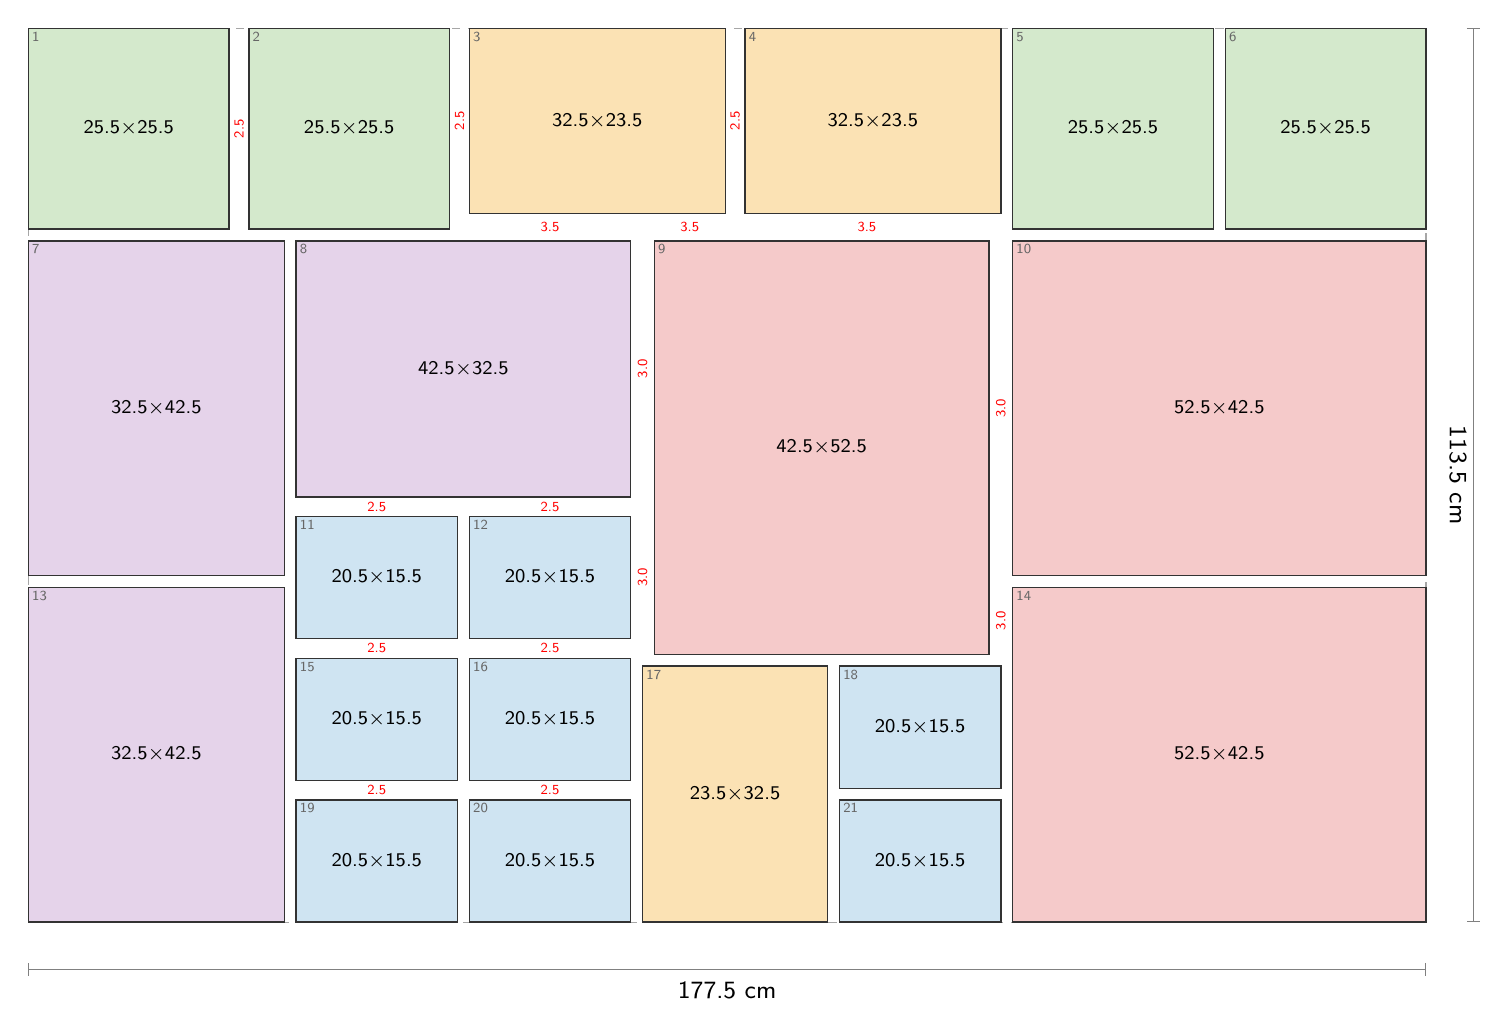
\begin{tikzpicture}[x=1mm, y=-1mm]
\draw[gray!70, dashed, line width=0.4pt] (0,0) rectangle (177.50,113.50);
\filldraw[fill=ft2, draw=black!80, line width=0.5pt] (0.00,0.00) rectangle (25.50,25.50);
\node[align=center, inner sep=0pt] at (12.75,12.75) {\scriptsize 25.5$\times$25.5};
\node[anchor=north west, inner sep=1.2pt, font=\tiny, text=black!60] at (0.00,0.00) {1};
\filldraw[fill=ft2, draw=black!80, line width=0.5pt] (28.00,0.00) rectangle (53.50,25.50);
\node[align=center, inner sep=0pt] at (40.75,12.75) {\scriptsize 25.5$\times$25.5};
\node[anchor=north west, inner sep=1.2pt, font=\tiny, text=black!60] at (28.00,0.00) {2};
\filldraw[fill=ft1, draw=black!80, line width=0.5pt] (56.00,0.00) rectangle (88.50,23.50);
\node[align=center, inner sep=0pt] at (72.25,11.75) {\scriptsize 32.5$\times$23.5};
\node[anchor=north west, inner sep=1.2pt, font=\tiny, text=black!60] at (56.00,0.00) {3};
\filldraw[fill=ft1, draw=black!80, line width=0.5pt] (91.00,0.00) rectangle (123.50,23.50);
\node[align=center, inner sep=0pt] at (107.25,11.75) {\scriptsize 32.5$\times$23.5};
\node[anchor=north west, inner sep=1.2pt, font=\tiny, text=black!60] at (91.00,0.00) {4};
\filldraw[fill=ft2, draw=black!80, line width=0.5pt] (125.00,0.00) rectangle (150.50,25.50);
\node[align=center, inner sep=0pt] at (137.75,12.75) {\scriptsize 25.5$\times$25.5};
\node[anchor=north west, inner sep=1.2pt, font=\tiny, text=black!60] at (125.00,0.00) {5};
\filldraw[fill=ft2, draw=black!80, line width=0.5pt] (152.00,0.00) rectangle (177.50,25.50);
\node[align=center, inner sep=0pt] at (164.75,12.75) {\scriptsize 25.5$\times$25.5};
\node[anchor=north west, inner sep=1.2pt, font=\tiny, text=black!60] at (152.00,0.00) {6};
\filldraw[fill=ft3, draw=black!80, line width=0.5pt] (0.00,27.00) rectangle (32.50,69.50);
\node[align=center, inner sep=0pt] at (16.25,48.25) {\scriptsize 32.5$\times$42.5};
\node[anchor=north west, inner sep=1.2pt, font=\tiny, text=black!60] at (0.00,27.00) {7};
\filldraw[fill=ft3, draw=black!80, line width=0.5pt] (34.00,27.00) rectangle (76.50,59.50);
\node[align=center, inner sep=0pt] at (55.25,43.25) {\scriptsize 42.5$\times$32.5};
\node[anchor=north west, inner sep=1.2pt, font=\tiny, text=black!60] at (34.00,27.00) {8};
\filldraw[fill=ft4, draw=black!80, line width=0.5pt] (79.50,27.00) rectangle (122.00,79.50);
\node[align=center, inner sep=0pt] at (100.75,53.25) {\scriptsize 42.5$\times$52.5};
\node[anchor=north west, inner sep=1.2pt, font=\tiny, text=black!60] at (79.50,27.00) {9};
\filldraw[fill=ft4, draw=black!80, line width=0.5pt] (125.00,27.00) rectangle (177.50,69.50);
\node[align=center, inner sep=0pt] at (151.25,48.25) {\scriptsize 52.5$\times$42.5};
\node[anchor=north west, inner sep=1.2pt, font=\tiny, text=black!60] at (125.00,27.00) {10};
\filldraw[fill=ft0, draw=black!80, line width=0.5pt] (34.00,62.00) rectangle (54.50,77.50);
\node[align=center, inner sep=0pt] at (44.25,69.75) {\scriptsize 20.5$\times$15.5};
\node[anchor=north west, inner sep=1.2pt, font=\tiny, text=black!60] at (34.00,62.00) {11};
\filldraw[fill=ft0, draw=black!80, line width=0.5pt] (56.00,62.00) rectangle (76.50,77.50);
\node[align=center, inner sep=0pt] at (66.25,69.75) {\scriptsize 20.5$\times$15.5};
\node[anchor=north west, inner sep=1.2pt, font=\tiny, text=black!60] at (56.00,62.00) {12};
\filldraw[fill=ft3, draw=black!80, line width=0.5pt] (0.00,71.00) rectangle (32.50,113.50);
\node[align=center, inner sep=0pt] at (16.25,92.25) {\scriptsize 32.5$\times$42.5};
\node[anchor=north west, inner sep=1.2pt, font=\tiny, text=black!60] at (0.00,71.00) {13};
\filldraw[fill=ft4, draw=black!80, line width=0.5pt] (125.00,71.00) rectangle (177.50,113.50);
\node[align=center, inner sep=0pt] at (151.25,92.25) {\scriptsize 52.5$\times$42.5};
\node[anchor=north west, inner sep=1.2pt, font=\tiny, text=black!60] at (125.00,71.00) {14};
\filldraw[fill=ft0, draw=black!80, line width=0.5pt] (34.00,80.00) rectangle (54.50,95.50);
\node[align=center, inner sep=0pt] at (44.25,87.75) {\scriptsize 20.5$\times$15.5};
\node[anchor=north west, inner sep=1.2pt, font=\tiny, text=black!60] at (34.00,80.00) {15};
\filldraw[fill=ft0, draw=black!80, line width=0.5pt] (56.00,80.00) rectangle (76.50,95.50);
\node[align=center, inner sep=0pt] at (66.25,87.75) {\scriptsize 20.5$\times$15.5};
\node[anchor=north west, inner sep=1.2pt, font=\tiny, text=black!60] at (56.00,80.00) {16};
\filldraw[fill=ft1, draw=black!80, line width=0.5pt] (78.00,81.00) rectangle (101.50,113.50);
\node[align=center, inner sep=0pt] at (89.75,97.25) {\scriptsize 23.5$\times$32.5};
\node[anchor=north west, inner sep=1.2pt, font=\tiny, text=black!60] at (78.00,81.00) {17};
\filldraw[fill=ft0, draw=black!80, line width=0.5pt] (103.00,81.00) rectangle (123.50,96.50);
\node[align=center, inner sep=0pt] at (113.25,88.75) {\scriptsize 20.5$\times$15.5};
\node[anchor=north west, inner sep=1.2pt, font=\tiny, text=black!60] at (103.00,81.00) {18};
\filldraw[fill=ft0, draw=black!80, line width=0.5pt] (34.00,98.00) rectangle (54.50,113.50);
\node[align=center, inner sep=0pt] at (44.25,105.75) {\scriptsize 20.5$\times$15.5};
\node[anchor=north west, inner sep=1.2pt, font=\tiny, text=black!60] at (34.00,98.00) {19};
\filldraw[fill=ft0, draw=black!80, line width=0.5pt] (56.00,98.00) rectangle (76.50,113.50);
\node[align=center, inner sep=0pt] at (66.25,105.75) {\scriptsize 20.5$\times$15.5};
\node[anchor=north west, inner sep=1.2pt, font=\tiny, text=black!60] at (56.00,98.00) {20};
\filldraw[fill=ft0, draw=black!80, line width=0.5pt] (103.00,98.00) rectangle (123.50,113.50);
\node[align=center, inner sep=0pt] at (113.25,105.75) {\scriptsize 20.5$\times$15.5};
\node[anchor=north west, inner sep=1.2pt, font=\tiny, text=black!60] at (103.00,98.00) {21};
\node[font=\tiny, text=red, fill=white, inner sep=0.3pt, rotate=90] at (26.75,12.75) {2.5};
\node[font=\tiny, text=red, fill=white, inner sep=0.3pt, rotate=90] at (54.75,11.75) {2.5};
\node[font=\tiny, text=red, fill=white, inner sep=0.3pt, rotate=90] at (89.75,11.75) {2.5};
\node[font=\tiny, text=red, fill=white, inner sep=0.3pt] at (66.25,25.25) {3.5};
\node[font=\tiny, text=red, fill=white, inner sep=0.3pt] at (84.00,25.25) {3.5};
\node[font=\tiny, text=red, fill=white, inner sep=0.3pt] at (106.50,25.25) {3.5};
\node[font=\tiny, text=red, fill=white, inner sep=0.3pt, rotate=90] at (78.00,43.25) {3.0};
\node[font=\tiny, text=red, fill=white, inner sep=0.3pt] at (44.25,60.75) {2.5};
\node[font=\tiny, text=red, fill=white, inner sep=0.3pt] at (66.25,60.75) {2.5};
\node[font=\tiny, text=red, fill=white, inner sep=0.3pt, rotate=90] at (123.50,48.25) {3.0};
\node[font=\tiny, text=red, fill=white, inner sep=0.3pt, rotate=90] at (123.50,75.25) {3.0};
\node[font=\tiny, text=red, fill=white, inner sep=0.3pt] at (44.25,78.75) {2.5};
\node[font=\tiny, text=red, fill=white, inner sep=0.3pt, rotate=90] at (78.00,69.75) {3.0};
\node[font=\tiny, text=red, fill=white, inner sep=0.3pt] at (66.25,78.75) {2.5};
\node[font=\tiny, text=red, fill=white, inner sep=0.3pt] at (44.25,96.75) {2.5};
\node[font=\tiny, text=red, fill=white, inner sep=0.3pt] at (66.25,96.75) {2.5};
\draw[Bar-Bar, gray] (0,119.50) -- (177.50,119.50) node[midway, below=1pt, font=\small, text=black] {177.5 cm};
\draw[Bar-Bar, gray] (183.50,0) -- (183.50,113.50) node[midway, right=1pt, font=\small, text=black, rotate=-90, anchor=north] {113.5 cm};
\end{tikzpicture}\\[4pt]
{\scriptsize Scale 1:10 (1 mm = 1 cm). Red numbers mark gaps that deviate from the nominal gap by more than 0.25 cm. Small grey numbers index the coordinate table.}
\end{minipage}\hfill
\begin{minipage}[t]{0.25\textwidth}\vspace{0pt}
\small
\begin{tabular}{@{}l l@{}}
\toprule
Outer size & 177.5 $\times$ 113.5 cm \\
Nominal gap & 1.5 cm \\
Actual gaps & 1.5 -- 3.5 cm \\
Max.\ deviation & 2.0 cm \\
Mean deviation & 0.51 cm \\
Border notches & none \\
Corners filled & 4 / 4 \\
Frames used & 21 of 28 \\
Large frames & {\scriptsize 3, touching 1$\times$ (52 cm), min.\ dist.\ 44 cm} \\
Entropy & 0.66 \\
\quad {\scriptsize mix / variety} & {\scriptsize 0.81 / 0.62} \\
\quad {\scriptsize stagger / lines} & {\scriptsize 0.44 / 0.75 (2 through)} \\
\bottomrule
\end{tabular}

\vspace{8pt}
\scriptsize
\begin{tabular}{@{}c l l r r@{}}
\toprule
 & outer w $\times$ h (cm) &  & used & have \\
\midrule
\tikz[baseline=-0.6ex]\fill[ft0,draw=black!60] (0,0) rectangle (1.2ex,1.2ex); & 20.5$\times$15.5 & L & 8 & 9 \\
\tikz[baseline=-0.6ex]\fill[ft0,draw=black!60] (0,0) rectangle (1.2ex,1.2ex); & 15.5$\times$20.5 & P & 0 & 2 \\
\tikz[baseline=-0.6ex]\fill[ft3,draw=black!60] (0,0) rectangle (1.2ex,1.2ex); & 32.5$\times$42.5 & P & 2 & 2 \\
\tikz[baseline=-0.6ex]\fill[ft3,draw=black!60] (0,0) rectangle (1.2ex,1.2ex); & 42.5$\times$32.5 & L & 1 & 1 \\
\tikz[baseline=-0.6ex]\fill[ft1,draw=black!60] (0,0) rectangle (1.2ex,1.2ex); & 32.5$\times$23.5 & L & 2 & 5 \\
\tikz[baseline=-0.6ex]\fill[ft1,draw=black!60] (0,0) rectangle (1.2ex,1.2ex); & 23.5$\times$32.5 & P & 1 & 1 \\
\tikz[baseline=-0.6ex]\fill[ft2,draw=black!60] (0,0) rectangle (1.2ex,1.2ex); & 25.5$\times$25.5 &  & 4 & 5 \\
\tikz[baseline=-0.6ex]\fill[ft4,draw=black!60] (0,0) rectangle (1.2ex,1.2ex); & 42.5$\times$52.5 & P & 1 & 1 \\
\tikz[baseline=-0.6ex]\fill[ft4,draw=black!60] (0,0) rectangle (1.2ex,1.2ex); & 52.5$\times$42.5 & L & 2 & 2 \\
\bottomrule
\end{tabular}

\vspace{8pt}
{\bfseries Positions} (top-left corner, cm)\\[2pt]
\tiny
\begin{tabular}{@{}r l r r@{}}
\toprule
\# & frame w $\times$ h & x & y \\
\midrule
1 & 25.5 $\times$ 25.5 & 0.0 & 0.0 \\
2 & 25.5 $\times$ 25.5 & 28.0 & 0.0 \\
3 & 32.5 $\times$ 23.5 & 56.0 & 0.0 \\
4 & 32.5 $\times$ 23.5 & 91.0 & 0.0 \\
5 & 25.5 $\times$ 25.5 & 125.0 & 0.0 \\
6 & 25.5 $\times$ 25.5 & 152.0 & 0.0 \\
7 & 32.5 $\times$ 42.5 & 0.0 & 27.0 \\
8 & 42.5 $\times$ 32.5 & 34.0 & 27.0 \\
9 & 42.5 $\times$ 52.5 & 79.5 & 27.0 \\
10 & 52.5 $\times$ 42.5 & 125.0 & 27.0 \\
11 & 20.5 $\times$ 15.5 & 34.0 & 62.0 \\
12 & 20.5 $\times$ 15.5 & 56.0 & 62.0 \\
13 & 32.5 $\times$ 42.5 & 0.0 & 71.0 \\
14 & 52.5 $\times$ 42.5 & 125.0 & 71.0 \\
15 & 20.5 $\times$ 15.5 & 34.0 & 80.0 \\
16 & 20.5 $\times$ 15.5 & 56.0 & 80.0 \\
17 & 23.5 $\times$ 32.5 & 78.0 & 81.0 \\
18 & 20.5 $\times$ 15.5 & 103.0 & 81.0 \\
19 & 20.5 $\times$ 15.5 & 34.0 & 98.0 \\
20 & 20.5 $\times$ 15.5 & 56.0 & 98.0 \\
21 & 20.5 $\times$ 15.5 & 103.0 & 98.0 \\
\bottomrule
\end{tabular}
\end{minipage}
\clearpage

\phantomsection\addcontentsline{toc}{subsection}{Layout 5: 181.5 \texorpdfstring{$\times$}{x} 126.5 cm, 25 frames, gap 2.5 cm, max.\ deviation 3.0 cm}
\label{lay:free-gap:5}
\begin{minipage}[t]{0.74\textwidth}\vspace{0pt}
{\LARGE\bfseries Layout 5}\hspace{1.5em}{\large 181.5 $\times$ 126.5 cm \quad gap 2.5 cm \quad 25 frames}\\[8pt]
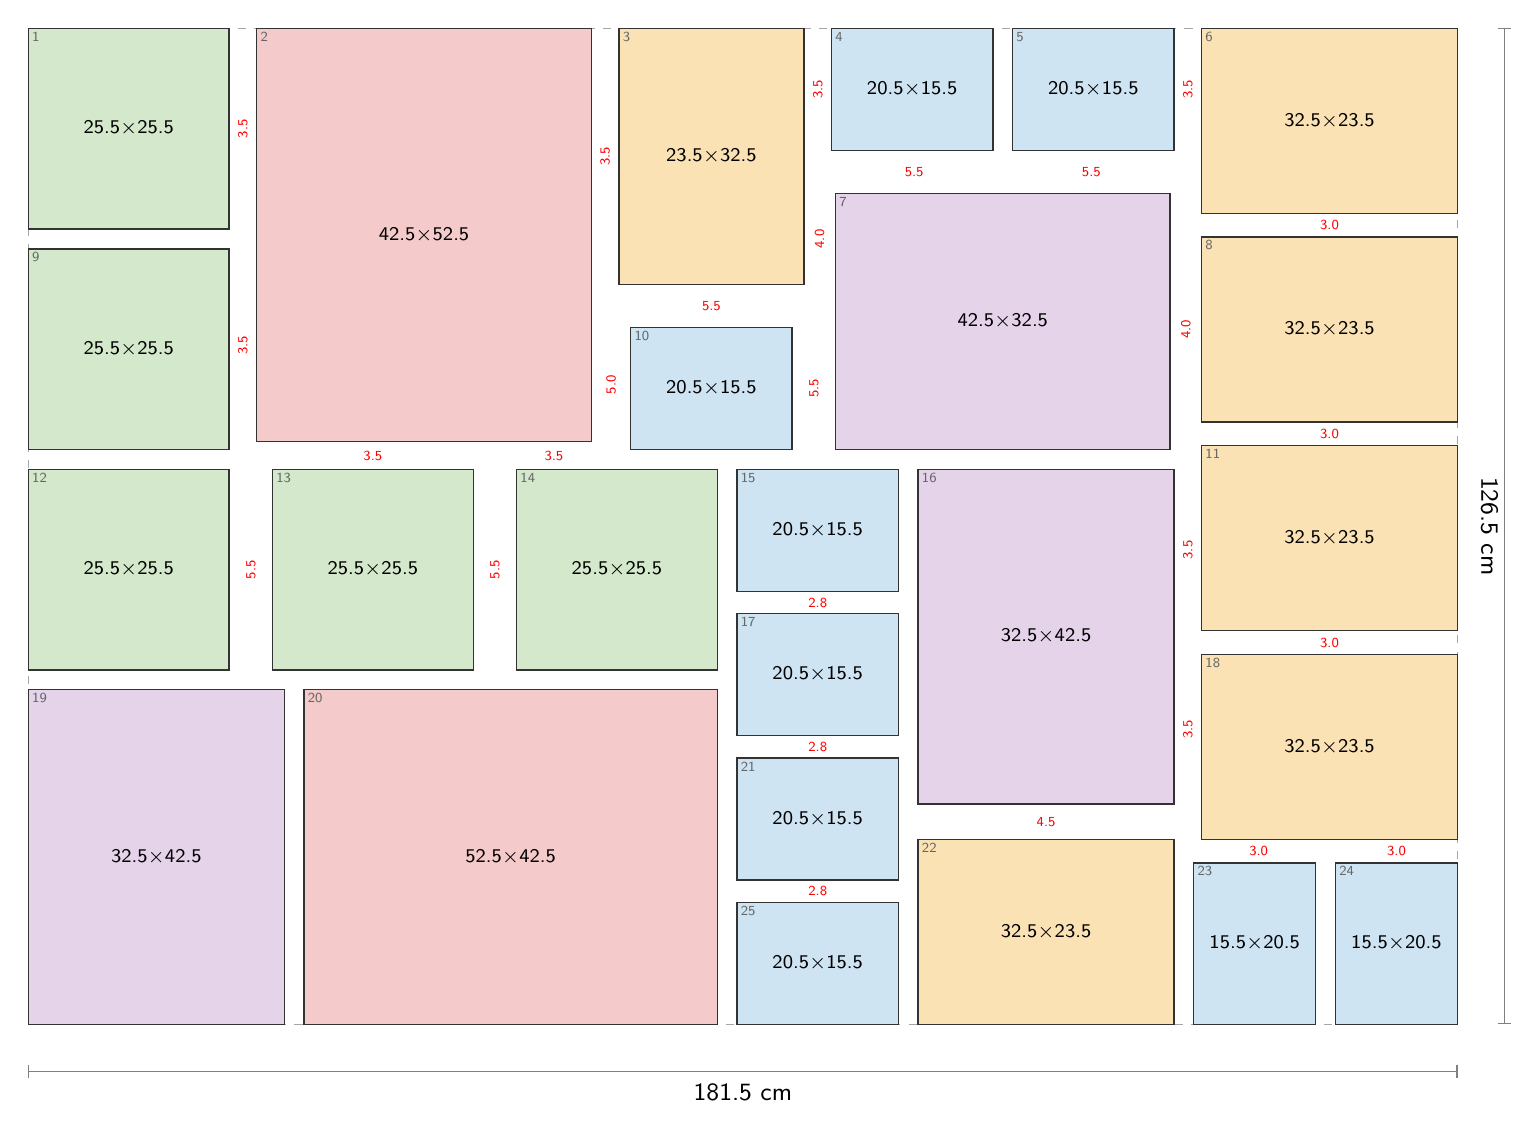
\begin{tikzpicture}[x=1mm, y=-1mm]
\draw[gray!70, dashed, line width=0.4pt] (0,0) rectangle (181.50,126.50);
\filldraw[fill=ft2, draw=black!80, line width=0.5pt] (0.00,0.00) rectangle (25.50,25.50);
\node[align=center, inner sep=0pt] at (12.75,12.75) {\scriptsize 25.5$\times$25.5};
\node[anchor=north west, inner sep=1.2pt, font=\tiny, text=black!60] at (0.00,0.00) {1};
\filldraw[fill=ft4, draw=black!80, line width=0.5pt] (29.00,0.00) rectangle (71.50,52.50);
\node[align=center, inner sep=0pt] at (50.25,26.25) {\scriptsize 42.5$\times$52.5};
\node[anchor=north west, inner sep=1.2pt, font=\tiny, text=black!60] at (29.00,0.00) {2};
\filldraw[fill=ft1, draw=black!80, line width=0.5pt] (75.00,0.00) rectangle (98.50,32.50);
\node[align=center, inner sep=0pt] at (86.75,16.25) {\scriptsize 23.5$\times$32.5};
\node[anchor=north west, inner sep=1.2pt, font=\tiny, text=black!60] at (75.00,0.00) {3};
\filldraw[fill=ft0, draw=black!80, line width=0.5pt] (102.00,0.00) rectangle (122.50,15.50);
\node[align=center, inner sep=0pt] at (112.25,7.75) {\scriptsize 20.5$\times$15.5};
\node[anchor=north west, inner sep=1.2pt, font=\tiny, text=black!60] at (102.00,0.00) {4};
\filldraw[fill=ft0, draw=black!80, line width=0.5pt] (125.00,0.00) rectangle (145.50,15.50);
\node[align=center, inner sep=0pt] at (135.25,7.75) {\scriptsize 20.5$\times$15.5};
\node[anchor=north west, inner sep=1.2pt, font=\tiny, text=black!60] at (125.00,0.00) {5};
\filldraw[fill=ft1, draw=black!80, line width=0.5pt] (149.00,0.00) rectangle (181.50,23.50);
\node[align=center, inner sep=0pt] at (165.25,11.75) {\scriptsize 32.5$\times$23.5};
\node[anchor=north west, inner sep=1.2pt, font=\tiny, text=black!60] at (149.00,0.00) {6};
\filldraw[fill=ft3, draw=black!80, line width=0.5pt] (102.50,21.00) rectangle (145.00,53.50);
\node[align=center, inner sep=0pt] at (123.75,37.25) {\scriptsize 42.5$\times$32.5};
\node[anchor=north west, inner sep=1.2pt, font=\tiny, text=black!60] at (102.50,21.00) {7};
\filldraw[fill=ft1, draw=black!80, line width=0.5pt] (149.00,26.50) rectangle (181.50,50.00);
\node[align=center, inner sep=0pt] at (165.25,38.25) {\scriptsize 32.5$\times$23.5};
\node[anchor=north west, inner sep=1.2pt, font=\tiny, text=black!60] at (149.00,26.50) {8};
\filldraw[fill=ft2, draw=black!80, line width=0.5pt] (0.00,28.00) rectangle (25.50,53.50);
\node[align=center, inner sep=0pt] at (12.75,40.75) {\scriptsize 25.5$\times$25.5};
\node[anchor=north west, inner sep=1.2pt, font=\tiny, text=black!60] at (0.00,28.00) {9};
\filldraw[fill=ft0, draw=black!80, line width=0.5pt] (76.50,38.00) rectangle (97.00,53.50);
\node[align=center, inner sep=0pt] at (86.75,45.75) {\scriptsize 20.5$\times$15.5};
\node[anchor=north west, inner sep=1.2pt, font=\tiny, text=black!60] at (76.50,38.00) {10};
\filldraw[fill=ft1, draw=black!80, line width=0.5pt] (149.00,53.00) rectangle (181.50,76.50);
\node[align=center, inner sep=0pt] at (165.25,64.75) {\scriptsize 32.5$\times$23.5};
\node[anchor=north west, inner sep=1.2pt, font=\tiny, text=black!60] at (149.00,53.00) {11};
\filldraw[fill=ft2, draw=black!80, line width=0.5pt] (0.00,56.00) rectangle (25.50,81.50);
\node[align=center, inner sep=0pt] at (12.75,68.75) {\scriptsize 25.5$\times$25.5};
\node[anchor=north west, inner sep=1.2pt, font=\tiny, text=black!60] at (0.00,56.00) {12};
\filldraw[fill=ft2, draw=black!80, line width=0.5pt] (31.00,56.00) rectangle (56.50,81.50);
\node[align=center, inner sep=0pt] at (43.75,68.75) {\scriptsize 25.5$\times$25.5};
\node[anchor=north west, inner sep=1.2pt, font=\tiny, text=black!60] at (31.00,56.00) {13};
\filldraw[fill=ft2, draw=black!80, line width=0.5pt] (62.00,56.00) rectangle (87.50,81.50);
\node[align=center, inner sep=0pt] at (74.75,68.75) {\scriptsize 25.5$\times$25.5};
\node[anchor=north west, inner sep=1.2pt, font=\tiny, text=black!60] at (62.00,56.00) {14};
\filldraw[fill=ft0, draw=black!80, line width=0.5pt] (90.00,56.00) rectangle (110.50,71.50);
\node[align=center, inner sep=0pt] at (100.25,63.75) {\scriptsize 20.5$\times$15.5};
\node[anchor=north west, inner sep=1.2pt, font=\tiny, text=black!60] at (90.00,56.00) {15};
\filldraw[fill=ft3, draw=black!80, line width=0.5pt] (113.00,56.00) rectangle (145.50,98.50);
\node[align=center, inner sep=0pt] at (129.25,77.25) {\scriptsize 32.5$\times$42.5};
\node[anchor=north west, inner sep=1.2pt, font=\tiny, text=black!60] at (113.00,56.00) {16};
\filldraw[fill=ft0, draw=black!80, line width=0.5pt] (90.00,74.33) rectangle (110.50,89.83);
\node[align=center, inner sep=0pt] at (100.25,82.08) {\scriptsize 20.5$\times$15.5};
\node[anchor=north west, inner sep=1.2pt, font=\tiny, text=black!60] at (90.00,74.33) {17};
\filldraw[fill=ft1, draw=black!80, line width=0.5pt] (149.00,79.50) rectangle (181.50,103.00);
\node[align=center, inner sep=0pt] at (165.25,91.25) {\scriptsize 32.5$\times$23.5};
\node[anchor=north west, inner sep=1.2pt, font=\tiny, text=black!60] at (149.00,79.50) {18};
\filldraw[fill=ft3, draw=black!80, line width=0.5pt] (0.00,84.00) rectangle (32.50,126.50);
\node[align=center, inner sep=0pt] at (16.25,105.25) {\scriptsize 32.5$\times$42.5};
\node[anchor=north west, inner sep=1.2pt, font=\tiny, text=black!60] at (0.00,84.00) {19};
\filldraw[fill=ft4, draw=black!80, line width=0.5pt] (35.00,84.00) rectangle (87.50,126.50);
\node[align=center, inner sep=0pt] at (61.25,105.25) {\scriptsize 52.5$\times$42.5};
\node[anchor=north west, inner sep=1.2pt, font=\tiny, text=black!60] at (35.00,84.00) {20};
\filldraw[fill=ft0, draw=black!80, line width=0.5pt] (90.00,92.67) rectangle (110.50,108.17);
\node[align=center, inner sep=0pt] at (100.25,100.42) {\scriptsize 20.5$\times$15.5};
\node[anchor=north west, inner sep=1.2pt, font=\tiny, text=black!60] at (90.00,92.67) {21};
\filldraw[fill=ft1, draw=black!80, line width=0.5pt] (113.00,103.00) rectangle (145.50,126.50);
\node[align=center, inner sep=0pt] at (129.25,114.75) {\scriptsize 32.5$\times$23.5};
\node[anchor=north west, inner sep=1.2pt, font=\tiny, text=black!60] at (113.00,103.00) {22};
\filldraw[fill=ft0, draw=black!80, line width=0.5pt] (148.00,106.00) rectangle (163.50,126.50);
\node[align=center, inner sep=0pt] at (155.75,116.25) {\scriptsize 15.5$\times$20.5};
\node[anchor=north west, inner sep=1.2pt, font=\tiny, text=black!60] at (148.00,106.00) {23};
\filldraw[fill=ft0, draw=black!80, line width=0.5pt] (166.00,106.00) rectangle (181.50,126.50);
\node[align=center, inner sep=0pt] at (173.75,116.25) {\scriptsize 15.5$\times$20.5};
\node[anchor=north west, inner sep=1.2pt, font=\tiny, text=black!60] at (166.00,106.00) {24};
\filldraw[fill=ft0, draw=black!80, line width=0.5pt] (90.00,111.00) rectangle (110.50,126.50);
\node[align=center, inner sep=0pt] at (100.25,118.75) {\scriptsize 20.5$\times$15.5};
\node[anchor=north west, inner sep=1.2pt, font=\tiny, text=black!60] at (90.00,111.00) {25};
\node[font=\tiny, text=red, fill=white, inner sep=0.3pt, rotate=90] at (27.25,12.75) {3.5};
\node[font=\tiny, text=red, fill=white, inner sep=0.3pt, rotate=90] at (73.25,16.25) {3.5};
\node[font=\tiny, text=red, fill=white, inner sep=0.3pt, rotate=90] at (74.00,45.25) {5.0};
\node[font=\tiny, text=red, fill=white, inner sep=0.3pt] at (43.75,54.25) {3.5};
\node[font=\tiny, text=red, fill=white, inner sep=0.3pt] at (66.75,54.25) {3.5};
\node[font=\tiny, text=red, fill=white, inner sep=0.3pt, rotate=90] at (100.25,7.75) {3.5};
\node[font=\tiny, text=red, fill=white, inner sep=0.3pt, rotate=90] at (100.50,26.75) {4.0};
\node[font=\tiny, text=red, fill=white, inner sep=0.3pt] at (86.75,35.25) {5.5};
\node[font=\tiny, text=red, fill=white, inner sep=0.3pt] at (112.50,18.25) {5.5};
\node[font=\tiny, text=red, fill=white, inner sep=0.3pt, rotate=90] at (147.25,7.75) {3.5};
\node[font=\tiny, text=red, fill=white, inner sep=0.3pt] at (135.00,18.25) {5.5};
\node[font=\tiny, text=red, fill=white, inner sep=0.3pt] at (165.25,25.00) {3.0};
\node[font=\tiny, text=red, fill=white, inner sep=0.3pt, rotate=90] at (147.00,38.25) {4.0};
\node[font=\tiny, text=red, fill=white, inner sep=0.3pt] at (165.25,51.50) {3.0};
\node[font=\tiny, text=red, fill=white, inner sep=0.3pt, rotate=90] at (27.25,40.25) {3.5};
\node[font=\tiny, text=red, fill=white, inner sep=0.3pt, rotate=90] at (99.75,45.75) {5.5};
\node[font=\tiny, text=red, fill=white, inner sep=0.3pt] at (165.25,78.00) {3.0};
\node[font=\tiny, text=red, fill=white, inner sep=0.3pt, rotate=90] at (28.25,68.75) {5.5};
\node[font=\tiny, text=red, fill=white, inner sep=0.3pt, rotate=90] at (59.25,68.75) {5.5};
\node[font=\tiny, text=red, fill=white, inner sep=0.3pt] at (100.25,72.92) {2.8};
\node[font=\tiny, text=red, fill=white, inner sep=0.3pt, rotate=90] at (147.25,66.25) {3.5};
\node[font=\tiny, text=red, fill=white, inner sep=0.3pt, rotate=90] at (147.25,89.00) {3.5};
\node[font=\tiny, text=red, fill=white, inner sep=0.3pt] at (129.25,100.75) {4.5};
\node[font=\tiny, text=red, fill=white, inner sep=0.3pt] at (100.25,91.25) {2.8};
\node[font=\tiny, text=red, fill=white, inner sep=0.3pt] at (156.25,104.50) {3.0};
\node[font=\tiny, text=red, fill=white, inner sep=0.3pt] at (173.75,104.50) {3.0};
\node[font=\tiny, text=red, fill=white, inner sep=0.3pt] at (100.25,109.58) {2.8};
\draw[Bar-Bar, gray] (0,132.50) -- (181.50,132.50) node[midway, below=1pt, font=\small, text=black] {181.5 cm};
\draw[Bar-Bar, gray] (187.50,0) -- (187.50,126.50) node[midway, right=1pt, font=\small, text=black, rotate=-90, anchor=north] {126.5 cm};
\end{tikzpicture}\\[4pt]
{\scriptsize Scale 1:10 (1 mm = 1 cm). Red numbers mark gaps that deviate from the nominal gap by more than 0.25 cm. Small grey numbers index the coordinate table.}
\end{minipage}\hfill
\begin{minipage}[t]{0.25\textwidth}\vspace{0pt}
\small
\begin{tabular}{@{}l l@{}}
\toprule
Outer size & 181.5 $\times$ 126.5 cm \\
Nominal gap & 2.5 cm \\
Actual gaps & 2.5 -- 5.5 cm \\
Max.\ deviation & 3.0 cm \\
Mean deviation & 0.76 cm \\
Border notches & none \\
Corners filled & 4 / 4 \\
Frames used & 25 of 28 \\
Large frames & {\scriptsize 2, not touching, min.\ dist.\ 80 cm} \\
Entropy & 0.79 \\
\quad {\scriptsize mix / variety} & {\scriptsize 0.87 / 0.72} \\
\quad {\scriptsize stagger / lines} & {\scriptsize 0.56 / 1.00 (1 through)} \\
\bottomrule
\end{tabular}

\vspace{8pt}
\scriptsize
\begin{tabular}{@{}c l l r r@{}}
\toprule
 & outer w $\times$ h (cm) &  & used & have \\
\midrule
\tikz[baseline=-0.6ex]\fill[ft0,draw=black!60] (0,0) rectangle (1.2ex,1.2ex); & 20.5$\times$15.5 & L & 7 & 9 \\
\tikz[baseline=-0.6ex]\fill[ft0,draw=black!60] (0,0) rectangle (1.2ex,1.2ex); & 15.5$\times$20.5 & P & 2 & 2 \\
\tikz[baseline=-0.6ex]\fill[ft3,draw=black!60] (0,0) rectangle (1.2ex,1.2ex); & 32.5$\times$42.5 & P & 2 & 2 \\
\tikz[baseline=-0.6ex]\fill[ft3,draw=black!60] (0,0) rectangle (1.2ex,1.2ex); & 42.5$\times$32.5 & L & 1 & 1 \\
\tikz[baseline=-0.6ex]\fill[ft1,draw=black!60] (0,0) rectangle (1.2ex,1.2ex); & 32.5$\times$23.5 & L & 5 & 5 \\
\tikz[baseline=-0.6ex]\fill[ft1,draw=black!60] (0,0) rectangle (1.2ex,1.2ex); & 23.5$\times$32.5 & P & 1 & 1 \\
\tikz[baseline=-0.6ex]\fill[ft2,draw=black!60] (0,0) rectangle (1.2ex,1.2ex); & 25.5$\times$25.5 &  & 5 & 5 \\
\tikz[baseline=-0.6ex]\fill[ft4,draw=black!60] (0,0) rectangle (1.2ex,1.2ex); & 42.5$\times$52.5 & P & 1 & 1 \\
\tikz[baseline=-0.6ex]\fill[ft4,draw=black!60] (0,0) rectangle (1.2ex,1.2ex); & 52.5$\times$42.5 & L & 1 & 2 \\
\bottomrule
\end{tabular}

\vspace{8pt}
{\bfseries Positions} (top-left corner, cm)\\[2pt]
\tiny
\begin{tabular}{@{}r l r r@{}}
\toprule
\# & frame w $\times$ h & x & y \\
\midrule
1 & 25.5 $\times$ 25.5 & 0.0 & 0.0 \\
2 & 42.5 $\times$ 52.5 & 29.0 & 0.0 \\
3 & 23.5 $\times$ 32.5 & 75.0 & 0.0 \\
4 & 20.5 $\times$ 15.5 & 102.0 & 0.0 \\
5 & 20.5 $\times$ 15.5 & 125.0 & 0.0 \\
6 & 32.5 $\times$ 23.5 & 149.0 & 0.0 \\
7 & 42.5 $\times$ 32.5 & 102.5 & 21.0 \\
8 & 32.5 $\times$ 23.5 & 149.0 & 26.5 \\
9 & 25.5 $\times$ 25.5 & 0.0 & 28.0 \\
10 & 20.5 $\times$ 15.5 & 76.5 & 38.0 \\
11 & 32.5 $\times$ 23.5 & 149.0 & 53.0 \\
12 & 25.5 $\times$ 25.5 & 0.0 & 56.0 \\
13 & 25.5 $\times$ 25.5 & 31.0 & 56.0 \\
14 & 25.5 $\times$ 25.5 & 62.0 & 56.0 \\
15 & 20.5 $\times$ 15.5 & 90.0 & 56.0 \\
16 & 32.5 $\times$ 42.5 & 113.0 & 56.0 \\
17 & 20.5 $\times$ 15.5 & 90.0 & 74.3 \\
18 & 32.5 $\times$ 23.5 & 149.0 & 79.5 \\
19 & 32.5 $\times$ 42.5 & 0.0 & 84.0 \\
20 & 52.5 $\times$ 42.5 & 35.0 & 84.0 \\
21 & 20.5 $\times$ 15.5 & 90.0 & 92.7 \\
22 & 32.5 $\times$ 23.5 & 113.0 & 103.0 \\
23 & 15.5 $\times$ 20.5 & 148.0 & 106.0 \\
24 & 15.5 $\times$ 20.5 & 166.0 & 106.0 \\
25 & 20.5 $\times$ 15.5 & 90.0 & 111.0 \\
\bottomrule
\end{tabular}
\end{minipage}
\clearpage

\phantomsection\addcontentsline{toc}{subsection}{Layout 6: 186.5 \texorpdfstring{$\times$}{x} 115.0 cm, 24 frames, gap 2 cm, max.\ deviation 2.2 cm}
\label{lay:free-gap:6}
\begin{minipage}[t]{0.74\textwidth}\vspace{0pt}
{\LARGE\bfseries Layout 6}\hspace{1.5em}{\large 186.5 $\times$ 115.0 cm \quad gap 2 cm \quad 24 frames}\\[8pt]
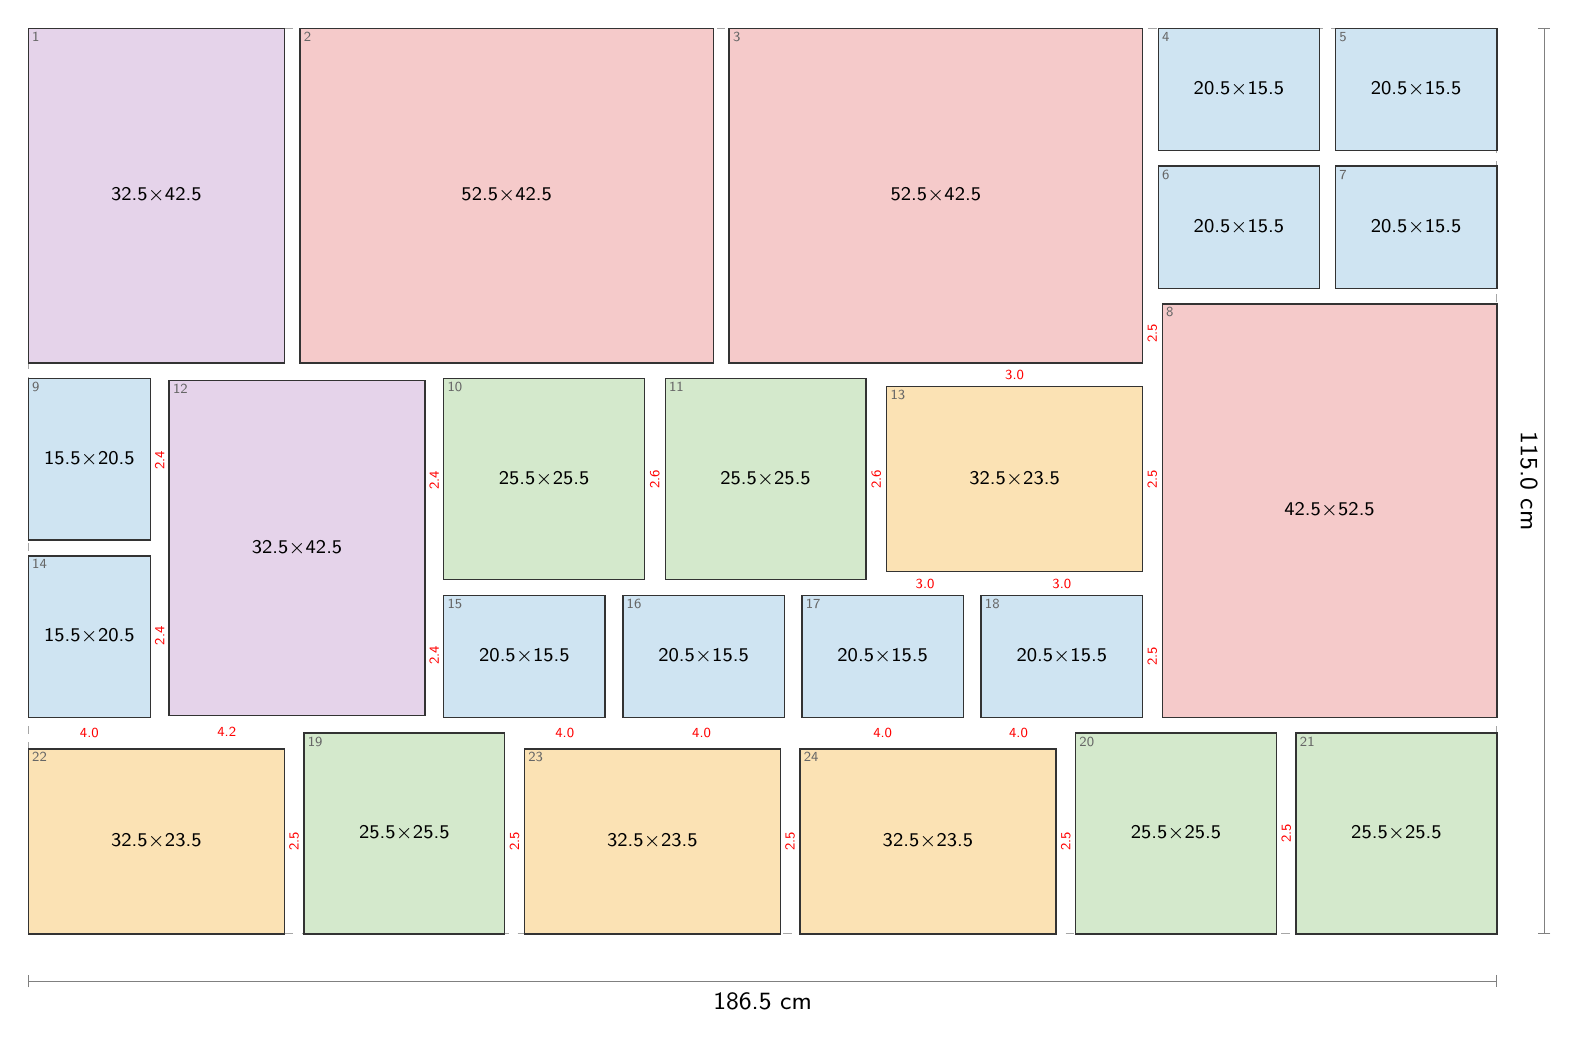
\begin{tikzpicture}[x=1mm, y=-1mm]
\draw[gray!70, dashed, line width=0.4pt] (0,0) rectangle (186.50,115.00);
\filldraw[fill=ft3, draw=black!80, line width=0.5pt] (0.00,0.00) rectangle (32.50,42.50);
\node[align=center, inner sep=0pt] at (16.25,21.25) {\scriptsize 32.5$\times$42.5};
\node[anchor=north west, inner sep=1.2pt, font=\tiny, text=black!60] at (0.00,0.00) {1};
\filldraw[fill=ft4, draw=black!80, line width=0.5pt] (34.50,0.00) rectangle (87.00,42.50);
\node[align=center, inner sep=0pt] at (60.75,21.25) {\scriptsize 52.5$\times$42.5};
\node[anchor=north west, inner sep=1.2pt, font=\tiny, text=black!60] at (34.50,0.00) {2};
\filldraw[fill=ft4, draw=black!80, line width=0.5pt] (89.00,0.00) rectangle (141.50,42.50);
\node[align=center, inner sep=0pt] at (115.25,21.25) {\scriptsize 52.5$\times$42.5};
\node[anchor=north west, inner sep=1.2pt, font=\tiny, text=black!60] at (89.00,0.00) {3};
\filldraw[fill=ft0, draw=black!80, line width=0.5pt] (143.50,0.00) rectangle (164.00,15.50);
\node[align=center, inner sep=0pt] at (153.75,7.75) {\scriptsize 20.5$\times$15.5};
\node[anchor=north west, inner sep=1.2pt, font=\tiny, text=black!60] at (143.50,0.00) {4};
\filldraw[fill=ft0, draw=black!80, line width=0.5pt] (166.00,0.00) rectangle (186.50,15.50);
\node[align=center, inner sep=0pt] at (176.25,7.75) {\scriptsize 20.5$\times$15.5};
\node[anchor=north west, inner sep=1.2pt, font=\tiny, text=black!60] at (166.00,0.00) {5};
\filldraw[fill=ft0, draw=black!80, line width=0.5pt] (143.50,17.50) rectangle (164.00,33.00);
\node[align=center, inner sep=0pt] at (153.75,25.25) {\scriptsize 20.5$\times$15.5};
\node[anchor=north west, inner sep=1.2pt, font=\tiny, text=black!60] at (143.50,17.50) {6};
\filldraw[fill=ft0, draw=black!80, line width=0.5pt] (166.00,17.50) rectangle (186.50,33.00);
\node[align=center, inner sep=0pt] at (176.25,25.25) {\scriptsize 20.5$\times$15.5};
\node[anchor=north west, inner sep=1.2pt, font=\tiny, text=black!60] at (166.00,17.50) {7};
\filldraw[fill=ft4, draw=black!80, line width=0.5pt] (144.00,35.00) rectangle (186.50,87.50);
\node[align=center, inner sep=0pt] at (165.25,61.25) {\scriptsize 42.5$\times$52.5};
\node[anchor=north west, inner sep=1.2pt, font=\tiny, text=black!60] at (144.00,35.00) {8};
\filldraw[fill=ft0, draw=black!80, line width=0.5pt] (0.00,44.50) rectangle (15.50,65.00);
\node[align=center, inner sep=0pt] at (7.75,54.75) {\scriptsize 15.5$\times$20.5};
\node[anchor=north west, inner sep=1.2pt, font=\tiny, text=black!60] at (0.00,44.50) {9};
\filldraw[fill=ft2, draw=black!80, line width=0.5pt] (52.75,44.50) rectangle (78.25,70.00);
\node[align=center, inner sep=0pt] at (65.50,57.25) {\scriptsize 25.5$\times$25.5};
\node[anchor=north west, inner sep=1.2pt, font=\tiny, text=black!60] at (52.75,44.50) {10};
\filldraw[fill=ft2, draw=black!80, line width=0.5pt] (80.88,44.50) rectangle (106.38,70.00);
\node[align=center, inner sep=0pt] at (93.62,57.25) {\scriptsize 25.5$\times$25.5};
\node[anchor=north west, inner sep=1.2pt, font=\tiny, text=black!60] at (80.88,44.50) {11};
\filldraw[fill=ft3, draw=black!80, line width=0.5pt] (17.88,44.75) rectangle (50.38,87.25);
\node[align=center, inner sep=0pt] at (34.12,66.00) {\scriptsize 32.5$\times$42.5};
\node[anchor=north west, inner sep=1.2pt, font=\tiny, text=black!60] at (17.88,44.75) {12};
\filldraw[fill=ft1, draw=black!80, line width=0.5pt] (109.00,45.50) rectangle (141.50,69.00);
\node[align=center, inner sep=0pt] at (125.25,57.25) {\scriptsize 32.5$\times$23.5};
\node[anchor=north west, inner sep=1.2pt, font=\tiny, text=black!60] at (109.00,45.50) {13};
\filldraw[fill=ft0, draw=black!80, line width=0.5pt] (0.00,67.00) rectangle (15.50,87.50);
\node[align=center, inner sep=0pt] at (7.75,77.25) {\scriptsize 15.5$\times$20.5};
\node[anchor=north west, inner sep=1.2pt, font=\tiny, text=black!60] at (0.00,67.00) {14};
\filldraw[fill=ft0, draw=black!80, line width=0.5pt] (52.75,72.00) rectangle (73.25,87.50);
\node[align=center, inner sep=0pt] at (63.00,79.75) {\scriptsize 20.5$\times$15.5};
\node[anchor=north west, inner sep=1.2pt, font=\tiny, text=black!60] at (52.75,72.00) {15};
\filldraw[fill=ft0, draw=black!80, line width=0.5pt] (75.50,72.00) rectangle (96.00,87.50);
\node[align=center, inner sep=0pt] at (85.75,79.75) {\scriptsize 20.5$\times$15.5};
\node[anchor=north west, inner sep=1.2pt, font=\tiny, text=black!60] at (75.50,72.00) {16};
\filldraw[fill=ft0, draw=black!80, line width=0.5pt] (98.25,72.00) rectangle (118.75,87.50);
\node[align=center, inner sep=0pt] at (108.50,79.75) {\scriptsize 20.5$\times$15.5};
\node[anchor=north west, inner sep=1.2pt, font=\tiny, text=black!60] at (98.25,72.00) {17};
\filldraw[fill=ft0, draw=black!80, line width=0.5pt] (121.00,72.00) rectangle (141.50,87.50);
\node[align=center, inner sep=0pt] at (131.25,79.75) {\scriptsize 20.5$\times$15.5};
\node[anchor=north west, inner sep=1.2pt, font=\tiny, text=black!60] at (121.00,72.00) {18};
\filldraw[fill=ft2, draw=black!80, line width=0.5pt] (35.00,89.50) rectangle (60.50,115.00);
\node[align=center, inner sep=0pt] at (47.75,102.25) {\scriptsize 25.5$\times$25.5};
\node[anchor=north west, inner sep=1.2pt, font=\tiny, text=black!60] at (35.00,89.50) {19};
\filldraw[fill=ft2, draw=black!80, line width=0.5pt] (133.00,89.50) rectangle (158.50,115.00);
\node[align=center, inner sep=0pt] at (145.75,102.25) {\scriptsize 25.5$\times$25.5};
\node[anchor=north west, inner sep=1.2pt, font=\tiny, text=black!60] at (133.00,89.50) {20};
\filldraw[fill=ft2, draw=black!80, line width=0.5pt] (161.00,89.50) rectangle (186.50,115.00);
\node[align=center, inner sep=0pt] at (173.75,102.25) {\scriptsize 25.5$\times$25.5};
\node[anchor=north west, inner sep=1.2pt, font=\tiny, text=black!60] at (161.00,89.50) {21};
\filldraw[fill=ft1, draw=black!80, line width=0.5pt] (0.00,91.50) rectangle (32.50,115.00);
\node[align=center, inner sep=0pt] at (16.25,103.25) {\scriptsize 32.5$\times$23.5};
\node[anchor=north west, inner sep=1.2pt, font=\tiny, text=black!60] at (0.00,91.50) {22};
\filldraw[fill=ft1, draw=black!80, line width=0.5pt] (63.00,91.50) rectangle (95.50,115.00);
\node[align=center, inner sep=0pt] at (79.25,103.25) {\scriptsize 32.5$\times$23.5};
\node[anchor=north west, inner sep=1.2pt, font=\tiny, text=black!60] at (63.00,91.50) {23};
\filldraw[fill=ft1, draw=black!80, line width=0.5pt] (98.00,91.50) rectangle (130.50,115.00);
\node[align=center, inner sep=0pt] at (114.25,103.25) {\scriptsize 32.5$\times$23.5};
\node[anchor=north west, inner sep=1.2pt, font=\tiny, text=black!60] at (98.00,91.50) {24};
\node[font=\tiny, text=red, fill=white, inner sep=0.3pt, rotate=90] at (142.75,38.75) {2.5};
\node[font=\tiny, text=red, fill=white, inner sep=0.3pt] at (125.25,44.00) {3.0};
\node[font=\tiny, text=red, fill=white, inner sep=0.3pt, rotate=90] at (16.69,54.88) {2.4};
\node[font=\tiny, text=red, fill=white, inner sep=0.3pt, rotate=90] at (79.56,57.25) {2.6};
\node[font=\tiny, text=red, fill=white, inner sep=0.3pt, rotate=90] at (107.69,57.25) {2.6};
\node[font=\tiny, text=red, fill=white, inner sep=0.3pt, rotate=90] at (51.56,57.38) {2.4};
\node[font=\tiny, text=red, fill=white, inner sep=0.3pt, rotate=90] at (51.56,79.62) {2.4};
\node[font=\tiny, text=red, fill=white, inner sep=0.3pt] at (25.19,89.38) {4.2};
\node[font=\tiny, text=red, fill=white, inner sep=0.3pt, rotate=90] at (142.75,57.25) {2.5};
\node[font=\tiny, text=red, fill=white, inner sep=0.3pt] at (113.88,70.50) {3.0};
\node[font=\tiny, text=red, fill=white, inner sep=0.3pt] at (131.25,70.50) {3.0};
\node[font=\tiny, text=red, fill=white, inner sep=0.3pt, rotate=90] at (16.69,77.12) {2.4};
\node[font=\tiny, text=red, fill=white, inner sep=0.3pt] at (7.75,89.50) {4.0};
\node[font=\tiny, text=red, fill=white, inner sep=0.3pt] at (68.12,89.50) {4.0};
\node[font=\tiny, text=red, fill=white, inner sep=0.3pt] at (85.50,89.50) {4.0};
\node[font=\tiny, text=red, fill=white, inner sep=0.3pt] at (108.50,89.50) {4.0};
\node[font=\tiny, text=red, fill=white, inner sep=0.3pt, rotate=90] at (142.75,79.75) {2.5};
\node[font=\tiny, text=red, fill=white, inner sep=0.3pt] at (125.75,89.50) {4.0};
\node[font=\tiny, text=red, fill=white, inner sep=0.3pt, rotate=90] at (61.75,103.25) {2.5};
\node[font=\tiny, text=red, fill=white, inner sep=0.3pt, rotate=90] at (159.75,102.25) {2.5};
\node[font=\tiny, text=red, fill=white, inner sep=0.3pt, rotate=90] at (33.75,103.25) {2.5};
\node[font=\tiny, text=red, fill=white, inner sep=0.3pt, rotate=90] at (96.75,103.25) {2.5};
\node[font=\tiny, text=red, fill=white, inner sep=0.3pt, rotate=90] at (131.75,103.25) {2.5};
\draw[Bar-Bar, gray] (0,121.00) -- (186.50,121.00) node[midway, below=1pt, font=\small, text=black] {186.5 cm};
\draw[Bar-Bar, gray] (192.50,0) -- (192.50,115.00) node[midway, right=1pt, font=\small, text=black, rotate=-90, anchor=north] {115.0 cm};
\end{tikzpicture}\\[4pt]
{\scriptsize Scale 1:10 (1 mm = 1 cm). Red numbers mark gaps that deviate from the nominal gap by more than 0.25 cm. Small grey numbers index the coordinate table.}
\end{minipage}\hfill
\begin{minipage}[t]{0.25\textwidth}\vspace{0pt}
\small
\begin{tabular}{@{}l l@{}}
\toprule
Outer size & 186.5 $\times$ 115.0 cm \\
Nominal gap & 2 cm \\
Actual gaps & 2.0 -- 4.2 cm \\
Max.\ deviation & 2.2 cm \\
Mean deviation & 0.46 cm \\
Border notches & left 4 cm \\
Corners filled & 4 / 4 \\
Frames used & 24 of 28 \\
Large frames & {\scriptsize 3, touching 2$\times$ (50 cm), min.\ dist.\ 54 cm} \\
Entropy & 0.76 \\
\quad {\scriptsize mix / variety} & {\scriptsize 0.79 / 0.71} \\
\quad {\scriptsize stagger / lines} & {\scriptsize 0.55 / 1.00 (1 through)} \\
\bottomrule
\end{tabular}

\vspace{8pt}
\scriptsize
\begin{tabular}{@{}c l l r r@{}}
\toprule
 & outer w $\times$ h (cm) &  & used & have \\
\midrule
\tikz[baseline=-0.6ex]\fill[ft0,draw=black!60] (0,0) rectangle (1.2ex,1.2ex); & 20.5$\times$15.5 & L & 8 & 9 \\
\tikz[baseline=-0.6ex]\fill[ft0,draw=black!60] (0,0) rectangle (1.2ex,1.2ex); & 15.5$\times$20.5 & P & 2 & 2 \\
\tikz[baseline=-0.6ex]\fill[ft3,draw=black!60] (0,0) rectangle (1.2ex,1.2ex); & 32.5$\times$42.5 & P & 2 & 2 \\
\tikz[baseline=-0.6ex]\fill[ft3,draw=black!60] (0,0) rectangle (1.2ex,1.2ex); & 42.5$\times$32.5 & L & 0 & 1 \\
\tikz[baseline=-0.6ex]\fill[ft1,draw=black!60] (0,0) rectangle (1.2ex,1.2ex); & 32.5$\times$23.5 & L & 4 & 5 \\
\tikz[baseline=-0.6ex]\fill[ft1,draw=black!60] (0,0) rectangle (1.2ex,1.2ex); & 23.5$\times$32.5 & P & 0 & 1 \\
\tikz[baseline=-0.6ex]\fill[ft2,draw=black!60] (0,0) rectangle (1.2ex,1.2ex); & 25.5$\times$25.5 &  & 5 & 5 \\
\tikz[baseline=-0.6ex]\fill[ft4,draw=black!60] (0,0) rectangle (1.2ex,1.2ex); & 42.5$\times$52.5 & P & 1 & 1 \\
\tikz[baseline=-0.6ex]\fill[ft4,draw=black!60] (0,0) rectangle (1.2ex,1.2ex); & 52.5$\times$42.5 & L & 2 & 2 \\
\bottomrule
\end{tabular}

\vspace{8pt}
{\bfseries Positions} (top-left corner, cm)\\[2pt]
\tiny
\begin{tabular}{@{}r l r r@{}}
\toprule
\# & frame w $\times$ h & x & y \\
\midrule
1 & 32.5 $\times$ 42.5 & 0.0 & 0.0 \\
2 & 52.5 $\times$ 42.5 & 34.5 & 0.0 \\
3 & 52.5 $\times$ 42.5 & 89.0 & 0.0 \\
4 & 20.5 $\times$ 15.5 & 143.5 & 0.0 \\
5 & 20.5 $\times$ 15.5 & 166.0 & 0.0 \\
6 & 20.5 $\times$ 15.5 & 143.5 & 17.5 \\
7 & 20.5 $\times$ 15.5 & 166.0 & 17.5 \\
8 & 42.5 $\times$ 52.5 & 144.0 & 35.0 \\
9 & 15.5 $\times$ 20.5 & 0.0 & 44.5 \\
10 & 25.5 $\times$ 25.5 & 52.8 & 44.5 \\
11 & 25.5 $\times$ 25.5 & 80.9 & 44.5 \\
12 & 32.5 $\times$ 42.5 & 17.9 & 44.8 \\
13 & 32.5 $\times$ 23.5 & 109.0 & 45.5 \\
14 & 15.5 $\times$ 20.5 & 0.0 & 67.0 \\
15 & 20.5 $\times$ 15.5 & 52.8 & 72.0 \\
16 & 20.5 $\times$ 15.5 & 75.5 & 72.0 \\
17 & 20.5 $\times$ 15.5 & 98.2 & 72.0 \\
18 & 20.5 $\times$ 15.5 & 121.0 & 72.0 \\
19 & 25.5 $\times$ 25.5 & 35.0 & 89.5 \\
20 & 25.5 $\times$ 25.5 & 133.0 & 89.5 \\
21 & 25.5 $\times$ 25.5 & 161.0 & 89.5 \\
22 & 32.5 $\times$ 23.5 & 0.0 & 91.5 \\
23 & 32.5 $\times$ 23.5 & 63.0 & 91.5 \\
24 & 32.5 $\times$ 23.5 & 98.0 & 91.5 \\
\bottomrule
\end{tabular}
\end{minipage}
\clearpage

\phantomsection\addcontentsline{toc}{subsection}{Layout 7: 180.5 \texorpdfstring{$\times$}{x} 128.5 cm, 24 frames, gap 3.5 cm, max.\ deviation 3.0 cm}
\label{lay:free-gap:7}
\begin{minipage}[t]{0.74\textwidth}\vspace{0pt}
{\LARGE\bfseries Layout 7}\hspace{1.5em}{\large 180.5 $\times$ 128.5 cm \quad gap 3.5 cm \quad 24 frames}\\[8pt]
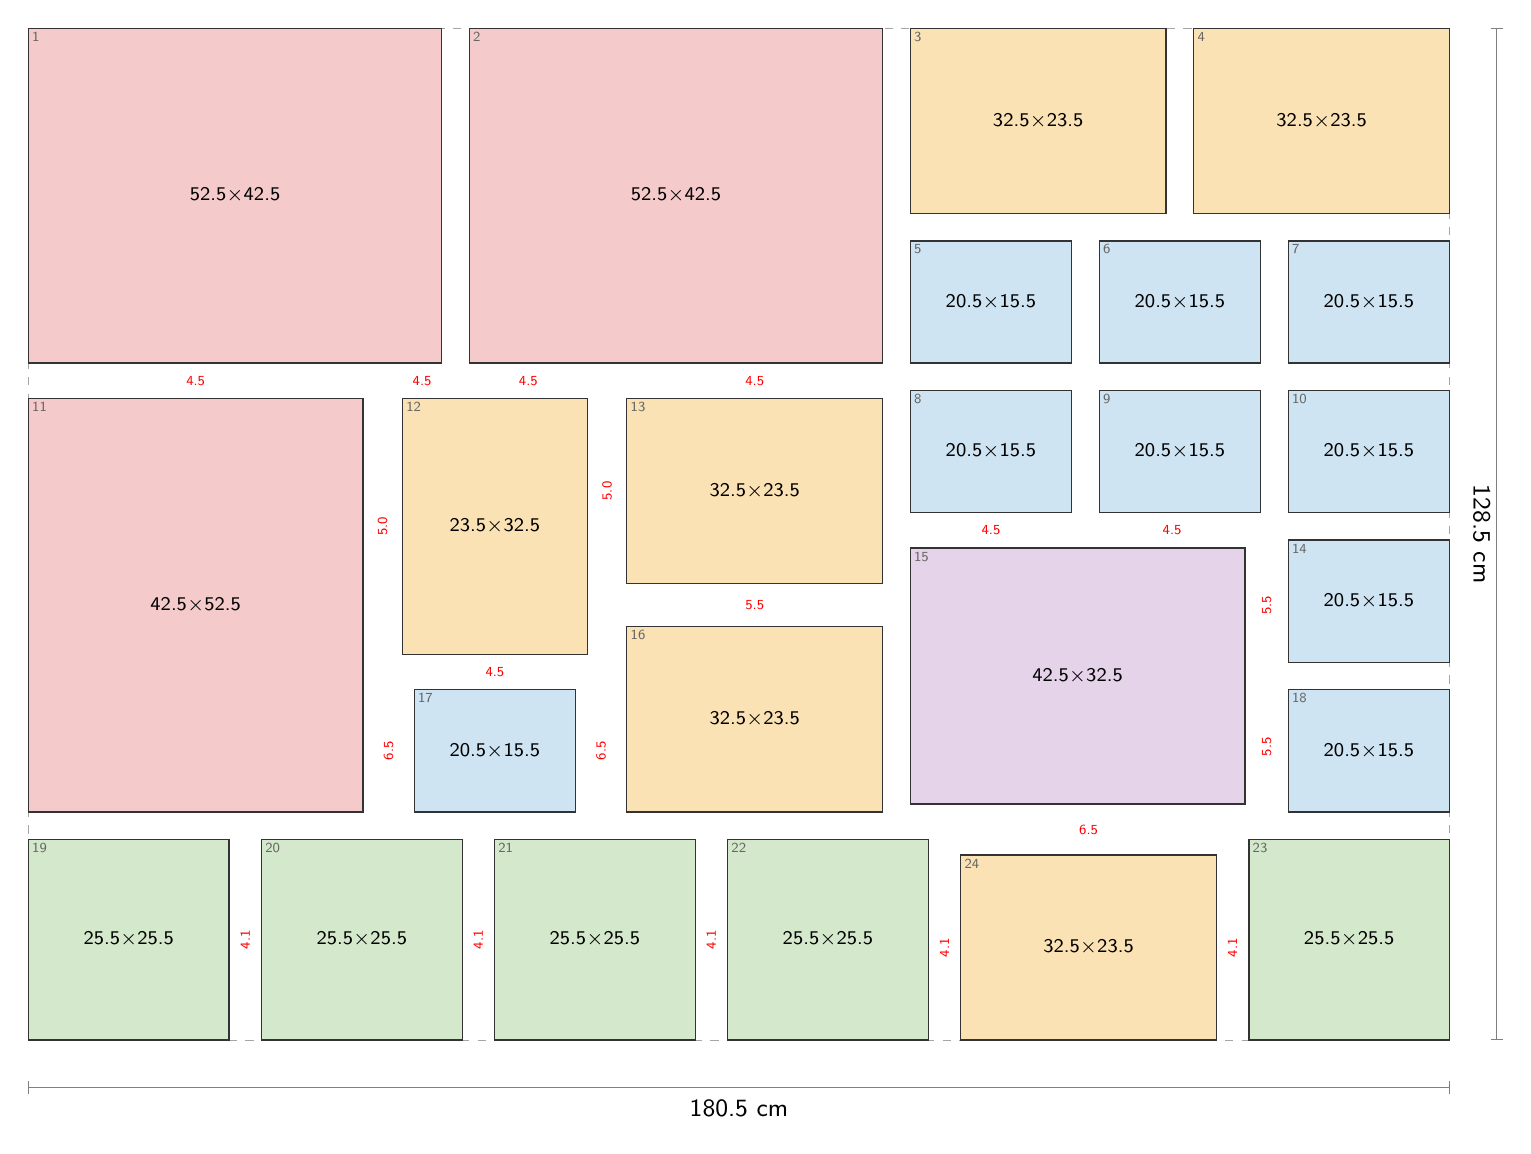
\begin{tikzpicture}[x=1mm, y=-1mm]
\draw[gray!70, dashed, line width=0.4pt] (0,0) rectangle (180.50,128.50);
\filldraw[fill=ft4, draw=black!80, line width=0.5pt] (0.00,0.00) rectangle (52.50,42.50);
\node[align=center, inner sep=0pt] at (26.25,21.25) {\scriptsize 52.5$\times$42.5};
\node[anchor=north west, inner sep=1.2pt, font=\tiny, text=black!60] at (0.00,0.00) {1};
\filldraw[fill=ft4, draw=black!80, line width=0.5pt] (56.00,0.00) rectangle (108.50,42.50);
\node[align=center, inner sep=0pt] at (82.25,21.25) {\scriptsize 52.5$\times$42.5};
\node[anchor=north west, inner sep=1.2pt, font=\tiny, text=black!60] at (56.00,0.00) {2};
\filldraw[fill=ft1, draw=black!80, line width=0.5pt] (112.00,0.00) rectangle (144.50,23.50);
\node[align=center, inner sep=0pt] at (128.25,11.75) {\scriptsize 32.5$\times$23.5};
\node[anchor=north west, inner sep=1.2pt, font=\tiny, text=black!60] at (112.00,0.00) {3};
\filldraw[fill=ft1, draw=black!80, line width=0.5pt] (148.00,0.00) rectangle (180.50,23.50);
\node[align=center, inner sep=0pt] at (164.25,11.75) {\scriptsize 32.5$\times$23.5};
\node[anchor=north west, inner sep=1.2pt, font=\tiny, text=black!60] at (148.00,0.00) {4};
\filldraw[fill=ft0, draw=black!80, line width=0.5pt] (112.00,27.00) rectangle (132.50,42.50);
\node[align=center, inner sep=0pt] at (122.25,34.75) {\scriptsize 20.5$\times$15.5};
\node[anchor=north west, inner sep=1.2pt, font=\tiny, text=black!60] at (112.00,27.00) {5};
\filldraw[fill=ft0, draw=black!80, line width=0.5pt] (136.00,27.00) rectangle (156.50,42.50);
\node[align=center, inner sep=0pt] at (146.25,34.75) {\scriptsize 20.5$\times$15.5};
\node[anchor=north west, inner sep=1.2pt, font=\tiny, text=black!60] at (136.00,27.00) {6};
\filldraw[fill=ft0, draw=black!80, line width=0.5pt] (160.00,27.00) rectangle (180.50,42.50);
\node[align=center, inner sep=0pt] at (170.25,34.75) {\scriptsize 20.5$\times$15.5};
\node[anchor=north west, inner sep=1.2pt, font=\tiny, text=black!60] at (160.00,27.00) {7};
\filldraw[fill=ft0, draw=black!80, line width=0.5pt] (112.00,46.00) rectangle (132.50,61.50);
\node[align=center, inner sep=0pt] at (122.25,53.75) {\scriptsize 20.5$\times$15.5};
\node[anchor=north west, inner sep=1.2pt, font=\tiny, text=black!60] at (112.00,46.00) {8};
\filldraw[fill=ft0, draw=black!80, line width=0.5pt] (136.00,46.00) rectangle (156.50,61.50);
\node[align=center, inner sep=0pt] at (146.25,53.75) {\scriptsize 20.5$\times$15.5};
\node[anchor=north west, inner sep=1.2pt, font=\tiny, text=black!60] at (136.00,46.00) {9};
\filldraw[fill=ft0, draw=black!80, line width=0.5pt] (160.00,46.00) rectangle (180.50,61.50);
\node[align=center, inner sep=0pt] at (170.25,53.75) {\scriptsize 20.5$\times$15.5};
\node[anchor=north west, inner sep=1.2pt, font=\tiny, text=black!60] at (160.00,46.00) {10};
\filldraw[fill=ft4, draw=black!80, line width=0.5pt] (0.00,47.00) rectangle (42.50,99.50);
\node[align=center, inner sep=0pt] at (21.25,73.25) {\scriptsize 42.5$\times$52.5};
\node[anchor=north west, inner sep=1.2pt, font=\tiny, text=black!60] at (0.00,47.00) {11};
\filldraw[fill=ft1, draw=black!80, line width=0.5pt] (47.50,47.00) rectangle (71.00,79.50);
\node[align=center, inner sep=0pt] at (59.25,63.25) {\scriptsize 23.5$\times$32.5};
\node[anchor=north west, inner sep=1.2pt, font=\tiny, text=black!60] at (47.50,47.00) {12};
\filldraw[fill=ft1, draw=black!80, line width=0.5pt] (76.00,47.00) rectangle (108.50,70.50);
\node[align=center, inner sep=0pt] at (92.25,58.75) {\scriptsize 32.5$\times$23.5};
\node[anchor=north west, inner sep=1.2pt, font=\tiny, text=black!60] at (76.00,47.00) {13};
\filldraw[fill=ft0, draw=black!80, line width=0.5pt] (160.00,65.00) rectangle (180.50,80.50);
\node[align=center, inner sep=0pt] at (170.25,72.75) {\scriptsize 20.5$\times$15.5};
\node[anchor=north west, inner sep=1.2pt, font=\tiny, text=black!60] at (160.00,65.00) {14};
\filldraw[fill=ft3, draw=black!80, line width=0.5pt] (112.00,66.00) rectangle (154.50,98.50);
\node[align=center, inner sep=0pt] at (133.25,82.25) {\scriptsize 42.5$\times$32.5};
\node[anchor=north west, inner sep=1.2pt, font=\tiny, text=black!60] at (112.00,66.00) {15};
\filldraw[fill=ft1, draw=black!80, line width=0.5pt] (76.00,76.00) rectangle (108.50,99.50);
\node[align=center, inner sep=0pt] at (92.25,87.75) {\scriptsize 32.5$\times$23.5};
\node[anchor=north west, inner sep=1.2pt, font=\tiny, text=black!60] at (76.00,76.00) {16};
\filldraw[fill=ft0, draw=black!80, line width=0.5pt] (49.00,84.00) rectangle (69.50,99.50);
\node[align=center, inner sep=0pt] at (59.25,91.75) {\scriptsize 20.5$\times$15.5};
\node[anchor=north west, inner sep=1.2pt, font=\tiny, text=black!60] at (49.00,84.00) {17};
\filldraw[fill=ft0, draw=black!80, line width=0.5pt] (160.00,84.00) rectangle (180.50,99.50);
\node[align=center, inner sep=0pt] at (170.25,91.75) {\scriptsize 20.5$\times$15.5};
\node[anchor=north west, inner sep=1.2pt, font=\tiny, text=black!60] at (160.00,84.00) {18};
\filldraw[fill=ft2, draw=black!80, line width=0.5pt] (0.00,103.00) rectangle (25.50,128.50);
\node[align=center, inner sep=0pt] at (12.75,115.75) {\scriptsize 25.5$\times$25.5};
\node[anchor=north west, inner sep=1.2pt, font=\tiny, text=black!60] at (0.00,103.00) {19};
\filldraw[fill=ft2, draw=black!80, line width=0.5pt] (29.60,103.00) rectangle (55.10,128.50);
\node[align=center, inner sep=0pt] at (42.35,115.75) {\scriptsize 25.5$\times$25.5};
\node[anchor=north west, inner sep=1.2pt, font=\tiny, text=black!60] at (29.60,103.00) {20};
\filldraw[fill=ft2, draw=black!80, line width=0.5pt] (59.20,103.00) rectangle (84.70,128.50);
\node[align=center, inner sep=0pt] at (71.95,115.75) {\scriptsize 25.5$\times$25.5};
\node[anchor=north west, inner sep=1.2pt, font=\tiny, text=black!60] at (59.20,103.00) {21};
\filldraw[fill=ft2, draw=black!80, line width=0.5pt] (88.80,103.00) rectangle (114.30,128.50);
\node[align=center, inner sep=0pt] at (101.55,115.75) {\scriptsize 25.5$\times$25.5};
\node[anchor=north west, inner sep=1.2pt, font=\tiny, text=black!60] at (88.80,103.00) {22};
\filldraw[fill=ft2, draw=black!80, line width=0.5pt] (155.00,103.00) rectangle (180.50,128.50);
\node[align=center, inner sep=0pt] at (167.75,115.75) {\scriptsize 25.5$\times$25.5};
\node[anchor=north west, inner sep=1.2pt, font=\tiny, text=black!60] at (155.00,103.00) {23};
\filldraw[fill=ft1, draw=black!80, line width=0.5pt] (118.40,105.00) rectangle (150.90,128.50);
\node[align=center, inner sep=0pt] at (134.65,116.75) {\scriptsize 32.5$\times$23.5};
\node[anchor=north west, inner sep=1.2pt, font=\tiny, text=black!60] at (118.40,105.00) {24};
\node[font=\tiny, text=red, fill=white, inner sep=0.3pt] at (21.25,44.75) {4.5};
\node[font=\tiny, text=red, fill=white, inner sep=0.3pt] at (50.00,44.75) {4.5};
\node[font=\tiny, text=red, fill=white, inner sep=0.3pt] at (63.50,44.75) {4.5};
\node[font=\tiny, text=red, fill=white, inner sep=0.3pt] at (92.25,44.75) {4.5};
\node[font=\tiny, text=red, fill=white, inner sep=0.3pt] at (122.25,63.75) {4.5};
\node[font=\tiny, text=red, fill=white, inner sep=0.3pt] at (145.25,63.75) {4.5};
\node[font=\tiny, text=red, fill=white, inner sep=0.3pt, rotate=90] at (45.00,63.25) {5.0};
\node[font=\tiny, text=red, fill=white, inner sep=0.3pt, rotate=90] at (45.75,91.75) {6.5};
\node[font=\tiny, text=red, fill=white, inner sep=0.3pt, rotate=90] at (73.50,58.75) {5.0};
\node[font=\tiny, text=red, fill=white, inner sep=0.3pt] at (59.25,81.75) {4.5};
\node[font=\tiny, text=red, fill=white, inner sep=0.3pt] at (92.25,73.25) {5.5};
\node[font=\tiny, text=red, fill=white, inner sep=0.3pt, rotate=90] at (157.25,73.25) {5.5};
\node[font=\tiny, text=red, fill=white, inner sep=0.3pt, rotate=90] at (157.25,91.25) {5.5};
\node[font=\tiny, text=red, fill=white, inner sep=0.3pt] at (134.65,101.75) {6.5};
\node[font=\tiny, text=red, fill=white, inner sep=0.3pt, rotate=90] at (72.75,91.75) {6.5};
\node[font=\tiny, text=red, fill=white, inner sep=0.3pt, rotate=90] at (27.55,115.75) {4.1};
\node[font=\tiny, text=red, fill=white, inner sep=0.3pt, rotate=90] at (57.15,115.75) {4.1};
\node[font=\tiny, text=red, fill=white, inner sep=0.3pt, rotate=90] at (86.75,115.75) {4.1};
\node[font=\tiny, text=red, fill=white, inner sep=0.3pt, rotate=90] at (116.35,116.75) {4.1};
\node[font=\tiny, text=red, fill=white, inner sep=0.3pt, rotate=90] at (152.95,116.75) {4.1};
\draw[Bar-Bar, gray] (0,134.50) -- (180.50,134.50) node[midway, below=1pt, font=\small, text=black] {180.5 cm};
\draw[Bar-Bar, gray] (186.50,0) -- (186.50,128.50) node[midway, right=1pt, font=\small, text=black, rotate=-90, anchor=north] {128.5 cm};
\end{tikzpicture}\\[4pt]
{\scriptsize Scale 1:10 (1 mm = 1 cm). Red numbers mark gaps that deviate from the nominal gap by more than 0.25 cm. Small grey numbers index the coordinate table.}
\end{minipage}\hfill
\begin{minipage}[t]{0.25\textwidth}\vspace{0pt}
\small
\begin{tabular}{@{}l l@{}}
\toprule
Outer size & 180.5 $\times$ 128.5 cm \\
Nominal gap & 3.5 cm \\
Actual gaps & 3.5 -- 6.5 cm \\
Max.\ deviation & 3.0 cm \\
Mean deviation & 0.61 cm \\
Border notches & none \\
Corners filled & 4 / 4 \\
Frames used & 24 of 28 \\
Large frames & {\scriptsize 3, touching 2$\times$ (85 cm), min.\ dist.\ 52 cm} \\
Entropy & 0.66 \\
\quad {\scriptsize mix / variety} & {\scriptsize 0.74 / 0.63} \\
\quad {\scriptsize stagger / lines} & {\scriptsize 0.50 / 0.75 (2 through)} \\
\bottomrule
\end{tabular}

\vspace{8pt}
\scriptsize
\begin{tabular}{@{}c l l r r@{}}
\toprule
 & outer w $\times$ h (cm) &  & used & have \\
\midrule
\tikz[baseline=-0.6ex]\fill[ft0,draw=black!60] (0,0) rectangle (1.2ex,1.2ex); & 20.5$\times$15.5 & L & 9 & 9 \\
\tikz[baseline=-0.6ex]\fill[ft0,draw=black!60] (0,0) rectangle (1.2ex,1.2ex); & 15.5$\times$20.5 & P & 0 & 2 \\
\tikz[baseline=-0.6ex]\fill[ft3,draw=black!60] (0,0) rectangle (1.2ex,1.2ex); & 32.5$\times$42.5 & P & 0 & 2 \\
\tikz[baseline=-0.6ex]\fill[ft3,draw=black!60] (0,0) rectangle (1.2ex,1.2ex); & 42.5$\times$32.5 & L & 1 & 1 \\
\tikz[baseline=-0.6ex]\fill[ft1,draw=black!60] (0,0) rectangle (1.2ex,1.2ex); & 32.5$\times$23.5 & L & 5 & 5 \\
\tikz[baseline=-0.6ex]\fill[ft1,draw=black!60] (0,0) rectangle (1.2ex,1.2ex); & 23.5$\times$32.5 & P & 1 & 1 \\
\tikz[baseline=-0.6ex]\fill[ft2,draw=black!60] (0,0) rectangle (1.2ex,1.2ex); & 25.5$\times$25.5 &  & 5 & 5 \\
\tikz[baseline=-0.6ex]\fill[ft4,draw=black!60] (0,0) rectangle (1.2ex,1.2ex); & 42.5$\times$52.5 & P & 1 & 1 \\
\tikz[baseline=-0.6ex]\fill[ft4,draw=black!60] (0,0) rectangle (1.2ex,1.2ex); & 52.5$\times$42.5 & L & 2 & 2 \\
\bottomrule
\end{tabular}

\vspace{8pt}
{\bfseries Positions} (top-left corner, cm)\\[2pt]
\tiny
\begin{tabular}{@{}r l r r@{}}
\toprule
\# & frame w $\times$ h & x & y \\
\midrule
1 & 52.5 $\times$ 42.5 & 0.0 & 0.0 \\
2 & 52.5 $\times$ 42.5 & 56.0 & 0.0 \\
3 & 32.5 $\times$ 23.5 & 112.0 & 0.0 \\
4 & 32.5 $\times$ 23.5 & 148.0 & 0.0 \\
5 & 20.5 $\times$ 15.5 & 112.0 & 27.0 \\
6 & 20.5 $\times$ 15.5 & 136.0 & 27.0 \\
7 & 20.5 $\times$ 15.5 & 160.0 & 27.0 \\
8 & 20.5 $\times$ 15.5 & 112.0 & 46.0 \\
9 & 20.5 $\times$ 15.5 & 136.0 & 46.0 \\
10 & 20.5 $\times$ 15.5 & 160.0 & 46.0 \\
11 & 42.5 $\times$ 52.5 & 0.0 & 47.0 \\
12 & 23.5 $\times$ 32.5 & 47.5 & 47.0 \\
13 & 32.5 $\times$ 23.5 & 76.0 & 47.0 \\
14 & 20.5 $\times$ 15.5 & 160.0 & 65.0 \\
15 & 42.5 $\times$ 32.5 & 112.0 & 66.0 \\
16 & 32.5 $\times$ 23.5 & 76.0 & 76.0 \\
17 & 20.5 $\times$ 15.5 & 49.0 & 84.0 \\
18 & 20.5 $\times$ 15.5 & 160.0 & 84.0 \\
19 & 25.5 $\times$ 25.5 & 0.0 & 103.0 \\
20 & 25.5 $\times$ 25.5 & 29.6 & 103.0 \\
21 & 25.5 $\times$ 25.5 & 59.2 & 103.0 \\
22 & 25.5 $\times$ 25.5 & 88.8 & 103.0 \\
23 & 25.5 $\times$ 25.5 & 155.0 & 103.0 \\
24 & 32.5 $\times$ 23.5 & 118.4 & 105.0 \\
\bottomrule
\end{tabular}
\end{minipage}
\clearpage

\phantomsection\addcontentsline{toc}{subsection}{Layout 8: 169.5 \texorpdfstring{$\times$}{x} 113.5 cm, 23 frames, gap 1.5 cm, max.\ deviation 2.5 cm}
\label{lay:free-gap:8}
\begin{minipage}[t]{0.74\textwidth}\vspace{0pt}
{\LARGE\bfseries Layout 8}\hspace{1.5em}{\large 169.5 $\times$ 113.5 cm \quad gap 1.5 cm \quad 23 frames}\\[8pt]
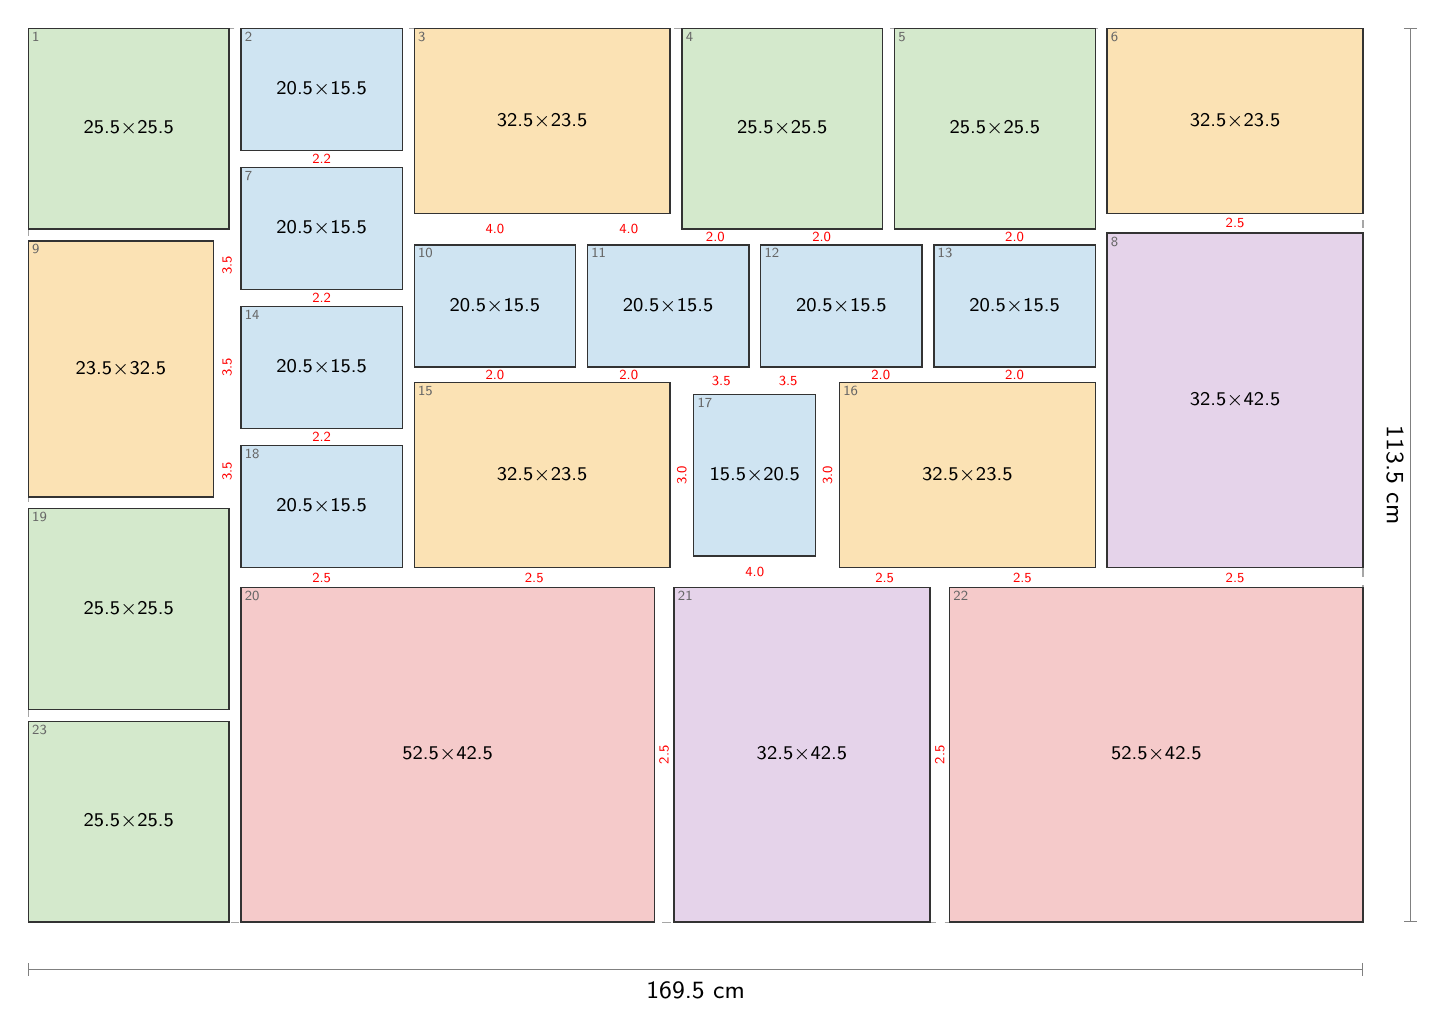
\begin{tikzpicture}[x=1mm, y=-1mm]
\draw[gray!70, dashed, line width=0.4pt] (0,0) rectangle (169.50,113.50);
\filldraw[fill=ft2, draw=black!80, line width=0.5pt] (0.00,0.00) rectangle (25.50,25.50);
\node[align=center, inner sep=0pt] at (12.75,12.75) {\scriptsize 25.5$\times$25.5};
\node[anchor=north west, inner sep=1.2pt, font=\tiny, text=black!60] at (0.00,0.00) {1};
\filldraw[fill=ft0, draw=black!80, line width=0.5pt] (27.00,0.00) rectangle (47.50,15.50);
\node[align=center, inner sep=0pt] at (37.25,7.75) {\scriptsize 20.5$\times$15.5};
\node[anchor=north west, inner sep=1.2pt, font=\tiny, text=black!60] at (27.00,0.00) {2};
\filldraw[fill=ft1, draw=black!80, line width=0.5pt] (49.00,0.00) rectangle (81.50,23.50);
\node[align=center, inner sep=0pt] at (65.25,11.75) {\scriptsize 32.5$\times$23.5};
\node[anchor=north west, inner sep=1.2pt, font=\tiny, text=black!60] at (49.00,0.00) {3};
\filldraw[fill=ft2, draw=black!80, line width=0.5pt] (83.00,0.00) rectangle (108.50,25.50);
\node[align=center, inner sep=0pt] at (95.75,12.75) {\scriptsize 25.5$\times$25.5};
\node[anchor=north west, inner sep=1.2pt, font=\tiny, text=black!60] at (83.00,0.00) {4};
\filldraw[fill=ft2, draw=black!80, line width=0.5pt] (110.00,0.00) rectangle (135.50,25.50);
\node[align=center, inner sep=0pt] at (122.75,12.75) {\scriptsize 25.5$\times$25.5};
\node[anchor=north west, inner sep=1.2pt, font=\tiny, text=black!60] at (110.00,0.00) {5};
\filldraw[fill=ft1, draw=black!80, line width=0.5pt] (137.00,0.00) rectangle (169.50,23.50);
\node[align=center, inner sep=0pt] at (153.25,11.75) {\scriptsize 32.5$\times$23.5};
\node[anchor=north west, inner sep=1.2pt, font=\tiny, text=black!60] at (137.00,0.00) {6};
\filldraw[fill=ft0, draw=black!80, line width=0.5pt] (27.00,17.67) rectangle (47.50,33.17);
\node[align=center, inner sep=0pt] at (37.25,25.42) {\scriptsize 20.5$\times$15.5};
\node[anchor=north west, inner sep=1.2pt, font=\tiny, text=black!60] at (27.00,17.67) {7};
\filldraw[fill=ft3, draw=black!80, line width=0.5pt] (137.00,26.00) rectangle (169.50,68.50);
\node[align=center, inner sep=0pt] at (153.25,47.25) {\scriptsize 32.5$\times$42.5};
\node[anchor=north west, inner sep=1.2pt, font=\tiny, text=black!60] at (137.00,26.00) {8};
\filldraw[fill=ft1, draw=black!80, line width=0.5pt] (0.00,27.00) rectangle (23.50,59.50);
\node[align=center, inner sep=0pt] at (11.75,43.25) {\scriptsize 23.5$\times$32.5};
\node[anchor=north west, inner sep=1.2pt, font=\tiny, text=black!60] at (0.00,27.00) {9};
\filldraw[fill=ft0, draw=black!80, line width=0.5pt] (49.00,27.50) rectangle (69.50,43.00);
\node[align=center, inner sep=0pt] at (59.25,35.25) {\scriptsize 20.5$\times$15.5};
\node[anchor=north west, inner sep=1.2pt, font=\tiny, text=black!60] at (49.00,27.50) {10};
\filldraw[fill=ft0, draw=black!80, line width=0.5pt] (71.00,27.50) rectangle (91.50,43.00);
\node[align=center, inner sep=0pt] at (81.25,35.25) {\scriptsize 20.5$\times$15.5};
\node[anchor=north west, inner sep=1.2pt, font=\tiny, text=black!60] at (71.00,27.50) {11};
\filldraw[fill=ft0, draw=black!80, line width=0.5pt] (93.00,27.50) rectangle (113.50,43.00);
\node[align=center, inner sep=0pt] at (103.25,35.25) {\scriptsize 20.5$\times$15.5};
\node[anchor=north west, inner sep=1.2pt, font=\tiny, text=black!60] at (93.00,27.50) {12};
\filldraw[fill=ft0, draw=black!80, line width=0.5pt] (115.00,27.50) rectangle (135.50,43.00);
\node[align=center, inner sep=0pt] at (125.25,35.25) {\scriptsize 20.5$\times$15.5};
\node[anchor=north west, inner sep=1.2pt, font=\tiny, text=black!60] at (115.00,27.50) {13};
\filldraw[fill=ft0, draw=black!80, line width=0.5pt] (27.00,35.33) rectangle (47.50,50.83);
\node[align=center, inner sep=0pt] at (37.25,43.08) {\scriptsize 20.5$\times$15.5};
\node[anchor=north west, inner sep=1.2pt, font=\tiny, text=black!60] at (27.00,35.33) {14};
\filldraw[fill=ft1, draw=black!80, line width=0.5pt] (49.00,45.00) rectangle (81.50,68.50);
\node[align=center, inner sep=0pt] at (65.25,56.75) {\scriptsize 32.5$\times$23.5};
\node[anchor=north west, inner sep=1.2pt, font=\tiny, text=black!60] at (49.00,45.00) {15};
\filldraw[fill=ft1, draw=black!80, line width=0.5pt] (103.00,45.00) rectangle (135.50,68.50);
\node[align=center, inner sep=0pt] at (119.25,56.75) {\scriptsize 32.5$\times$23.5};
\node[anchor=north west, inner sep=1.2pt, font=\tiny, text=black!60] at (103.00,45.00) {16};
\filldraw[fill=ft0, draw=black!80, line width=0.5pt] (84.50,46.50) rectangle (100.00,67.00);
\node[align=center, inner sep=0pt] at (92.25,56.75) {\scriptsize 15.5$\times$20.5};
\node[anchor=north west, inner sep=1.2pt, font=\tiny, text=black!60] at (84.50,46.50) {17};
\filldraw[fill=ft0, draw=black!80, line width=0.5pt] (27.00,53.00) rectangle (47.50,68.50);
\node[align=center, inner sep=0pt] at (37.25,60.75) {\scriptsize 20.5$\times$15.5};
\node[anchor=north west, inner sep=1.2pt, font=\tiny, text=black!60] at (27.00,53.00) {18};
\filldraw[fill=ft2, draw=black!80, line width=0.5pt] (0.00,61.00) rectangle (25.50,86.50);
\node[align=center, inner sep=0pt] at (12.75,73.75) {\scriptsize 25.5$\times$25.5};
\node[anchor=north west, inner sep=1.2pt, font=\tiny, text=black!60] at (0.00,61.00) {19};
\filldraw[fill=ft4, draw=black!80, line width=0.5pt] (27.00,71.00) rectangle (79.50,113.50);
\node[align=center, inner sep=0pt] at (53.25,92.25) {\scriptsize 52.5$\times$42.5};
\node[anchor=north west, inner sep=1.2pt, font=\tiny, text=black!60] at (27.00,71.00) {20};
\filldraw[fill=ft3, draw=black!80, line width=0.5pt] (82.00,71.00) rectangle (114.50,113.50);
\node[align=center, inner sep=0pt] at (98.25,92.25) {\scriptsize 32.5$\times$42.5};
\node[anchor=north west, inner sep=1.2pt, font=\tiny, text=black!60] at (82.00,71.00) {21};
\filldraw[fill=ft4, draw=black!80, line width=0.5pt] (117.00,71.00) rectangle (169.50,113.50);
\node[align=center, inner sep=0pt] at (143.25,92.25) {\scriptsize 52.5$\times$42.5};
\node[anchor=north west, inner sep=1.2pt, font=\tiny, text=black!60] at (117.00,71.00) {22};
\filldraw[fill=ft2, draw=black!80, line width=0.5pt] (0.00,88.00) rectangle (25.50,113.50);
\node[align=center, inner sep=0pt] at (12.75,100.75) {\scriptsize 25.5$\times$25.5};
\node[anchor=north west, inner sep=1.2pt, font=\tiny, text=black!60] at (0.00,88.00) {23};
\node[font=\tiny, text=red, fill=white, inner sep=0.3pt] at (37.25,16.58) {2.2};
\node[font=\tiny, text=red, fill=white, inner sep=0.3pt] at (59.25,25.50) {4.0};
\node[font=\tiny, text=red, fill=white, inner sep=0.3pt] at (76.25,25.50) {4.0};
\node[font=\tiny, text=red, fill=white, inner sep=0.3pt] at (87.25,26.50) {2.0};
\node[font=\tiny, text=red, fill=white, inner sep=0.3pt] at (100.75,26.50) {2.0};
\node[font=\tiny, text=red, fill=white, inner sep=0.3pt] at (125.25,26.50) {2.0};
\node[font=\tiny, text=red, fill=white, inner sep=0.3pt] at (153.25,24.75) {2.5};
\node[font=\tiny, text=red, fill=white, inner sep=0.3pt] at (37.25,34.25) {2.2};
\node[font=\tiny, text=red, fill=white, inner sep=0.3pt] at (153.25,69.75) {2.5};
\node[font=\tiny, text=red, fill=white, inner sep=0.3pt, rotate=90] at (25.25,30.08) {3.5};
\node[font=\tiny, text=red, fill=white, inner sep=0.3pt, rotate=90] at (25.25,43.08) {3.5};
\node[font=\tiny, text=red, fill=white, inner sep=0.3pt, rotate=90] at (25.25,56.25) {3.5};
\node[font=\tiny, text=red, fill=white, inner sep=0.3pt] at (59.25,44.00) {2.0};
\node[font=\tiny, text=red, fill=white, inner sep=0.3pt] at (76.25,44.00) {2.0};
\node[font=\tiny, text=red, fill=white, inner sep=0.3pt] at (88.00,44.75) {3.5};
\node[font=\tiny, text=red, fill=white, inner sep=0.3pt] at (108.25,44.00) {2.0};
\node[font=\tiny, text=red, fill=white, inner sep=0.3pt] at (96.50,44.75) {3.5};
\node[font=\tiny, text=red, fill=white, inner sep=0.3pt] at (125.25,44.00) {2.0};
\node[font=\tiny, text=red, fill=white, inner sep=0.3pt] at (37.25,51.92) {2.2};
\node[font=\tiny, text=red, fill=white, inner sep=0.3pt, rotate=90] at (83.00,56.75) {3.0};
\node[font=\tiny, text=red, fill=white, inner sep=0.3pt] at (64.25,69.75) {2.5};
\node[font=\tiny, text=red, fill=white, inner sep=0.3pt] at (108.75,69.75) {2.5};
\node[font=\tiny, text=red, fill=white, inner sep=0.3pt] at (126.25,69.75) {2.5};
\node[font=\tiny, text=red, fill=white, inner sep=0.3pt, rotate=90] at (101.50,56.75) {3.0};
\node[font=\tiny, text=red, fill=white, inner sep=0.3pt] at (92.25,69.00) {4.0};
\node[font=\tiny, text=red, fill=white, inner sep=0.3pt] at (37.25,69.75) {2.5};
\node[font=\tiny, text=red, fill=white, inner sep=0.3pt, rotate=90] at (80.75,92.25) {2.5};
\node[font=\tiny, text=red, fill=white, inner sep=0.3pt, rotate=90] at (115.75,92.25) {2.5};
\draw[Bar-Bar, gray] (0,119.50) -- (169.50,119.50) node[midway, below=1pt, font=\small, text=black] {169.5 cm};
\draw[Bar-Bar, gray] (175.50,0) -- (175.50,113.50) node[midway, right=1pt, font=\small, text=black, rotate=-90, anchor=north] {113.5 cm};
\end{tikzpicture}\\[4pt]
{\scriptsize Scale 1:10 (1 mm = 1 cm). Red numbers mark gaps that deviate from the nominal gap by more than 0.25 cm. Small grey numbers index the coordinate table.}
\end{minipage}\hfill
\begin{minipage}[t]{0.25\textwidth}\vspace{0pt}
\small
\begin{tabular}{@{}l l@{}}
\toprule
Outer size & 169.5 $\times$ 113.5 cm \\
Nominal gap & 1.5 cm \\
Actual gaps & 1.5 -- 4.0 cm \\
Max.\ deviation & 2.5 cm \\
Mean deviation & 0.68 cm \\
Border notches & none \\
Corners filled & 4 / 4 \\
Frames used & 23 of 28 \\
Large frames & {\scriptsize 2, not touching, min.\ dist.\ 90 cm} \\
Entropy & 0.76 \\
\quad {\scriptsize mix / variety} & {\scriptsize 0.77 / 0.75} \\
\quad {\scriptsize stagger / lines} & {\scriptsize 0.53 / 1.00 (1 through)} \\
\bottomrule
\end{tabular}

\vspace{8pt}
\scriptsize
\begin{tabular}{@{}c l l r r@{}}
\toprule
 & outer w $\times$ h (cm) &  & used & have \\
\midrule
\tikz[baseline=-0.6ex]\fill[ft0,draw=black!60] (0,0) rectangle (1.2ex,1.2ex); & 20.5$\times$15.5 & L & 8 & 9 \\
\tikz[baseline=-0.6ex]\fill[ft0,draw=black!60] (0,0) rectangle (1.2ex,1.2ex); & 15.5$\times$20.5 & P & 1 & 2 \\
\tikz[baseline=-0.6ex]\fill[ft3,draw=black!60] (0,0) rectangle (1.2ex,1.2ex); & 32.5$\times$42.5 & P & 2 & 2 \\
\tikz[baseline=-0.6ex]\fill[ft3,draw=black!60] (0,0) rectangle (1.2ex,1.2ex); & 42.5$\times$32.5 & L & 0 & 1 \\
\tikz[baseline=-0.6ex]\fill[ft1,draw=black!60] (0,0) rectangle (1.2ex,1.2ex); & 32.5$\times$23.5 & L & 4 & 5 \\
\tikz[baseline=-0.6ex]\fill[ft1,draw=black!60] (0,0) rectangle (1.2ex,1.2ex); & 23.5$\times$32.5 & P & 1 & 1 \\
\tikz[baseline=-0.6ex]\fill[ft2,draw=black!60] (0,0) rectangle (1.2ex,1.2ex); & 25.5$\times$25.5 &  & 5 & 5 \\
\tikz[baseline=-0.6ex]\fill[ft4,draw=black!60] (0,0) rectangle (1.2ex,1.2ex); & 42.5$\times$52.5 & P & 0 & 1 \\
\tikz[baseline=-0.6ex]\fill[ft4,draw=black!60] (0,0) rectangle (1.2ex,1.2ex); & 52.5$\times$42.5 & L & 2 & 2 \\
\bottomrule
\end{tabular}

\vspace{8pt}
{\bfseries Positions} (top-left corner, cm)\\[2pt]
\tiny
\begin{tabular}{@{}r l r r@{}}
\toprule
\# & frame w $\times$ h & x & y \\
\midrule
1 & 25.5 $\times$ 25.5 & 0.0 & 0.0 \\
2 & 20.5 $\times$ 15.5 & 27.0 & 0.0 \\
3 & 32.5 $\times$ 23.5 & 49.0 & 0.0 \\
4 & 25.5 $\times$ 25.5 & 83.0 & 0.0 \\
5 & 25.5 $\times$ 25.5 & 110.0 & 0.0 \\
6 & 32.5 $\times$ 23.5 & 137.0 & 0.0 \\
7 & 20.5 $\times$ 15.5 & 27.0 & 17.7 \\
8 & 32.5 $\times$ 42.5 & 137.0 & 26.0 \\
9 & 23.5 $\times$ 32.5 & 0.0 & 27.0 \\
10 & 20.5 $\times$ 15.5 & 49.0 & 27.5 \\
11 & 20.5 $\times$ 15.5 & 71.0 & 27.5 \\
12 & 20.5 $\times$ 15.5 & 93.0 & 27.5 \\
13 & 20.5 $\times$ 15.5 & 115.0 & 27.5 \\
14 & 20.5 $\times$ 15.5 & 27.0 & 35.3 \\
15 & 32.5 $\times$ 23.5 & 49.0 & 45.0 \\
16 & 32.5 $\times$ 23.5 & 103.0 & 45.0 \\
17 & 15.5 $\times$ 20.5 & 84.5 & 46.5 \\
18 & 20.5 $\times$ 15.5 & 27.0 & 53.0 \\
19 & 25.5 $\times$ 25.5 & 0.0 & 61.0 \\
20 & 52.5 $\times$ 42.5 & 27.0 & 71.0 \\
21 & 32.5 $\times$ 42.5 & 82.0 & 71.0 \\
22 & 52.5 $\times$ 42.5 & 117.0 & 71.0 \\
23 & 25.5 $\times$ 25.5 & 0.0 & 88.0 \\
\bottomrule
\end{tabular}
\end{minipage}
\clearpage

\phantomsection\addcontentsline{toc}{subsection}{Layout 9: 184.0 \texorpdfstring{$\times$}{x} 115.0 cm, 23 frames, gap 2 cm, max.\ deviation 2.2 cm}
\label{lay:free-gap:9}
\begin{minipage}[t]{0.74\textwidth}\vspace{0pt}
{\LARGE\bfseries Layout 9}\hspace{1.5em}{\large 184.0 $\times$ 115.0 cm \quad gap 2 cm \quad 23 frames}\\[8pt]
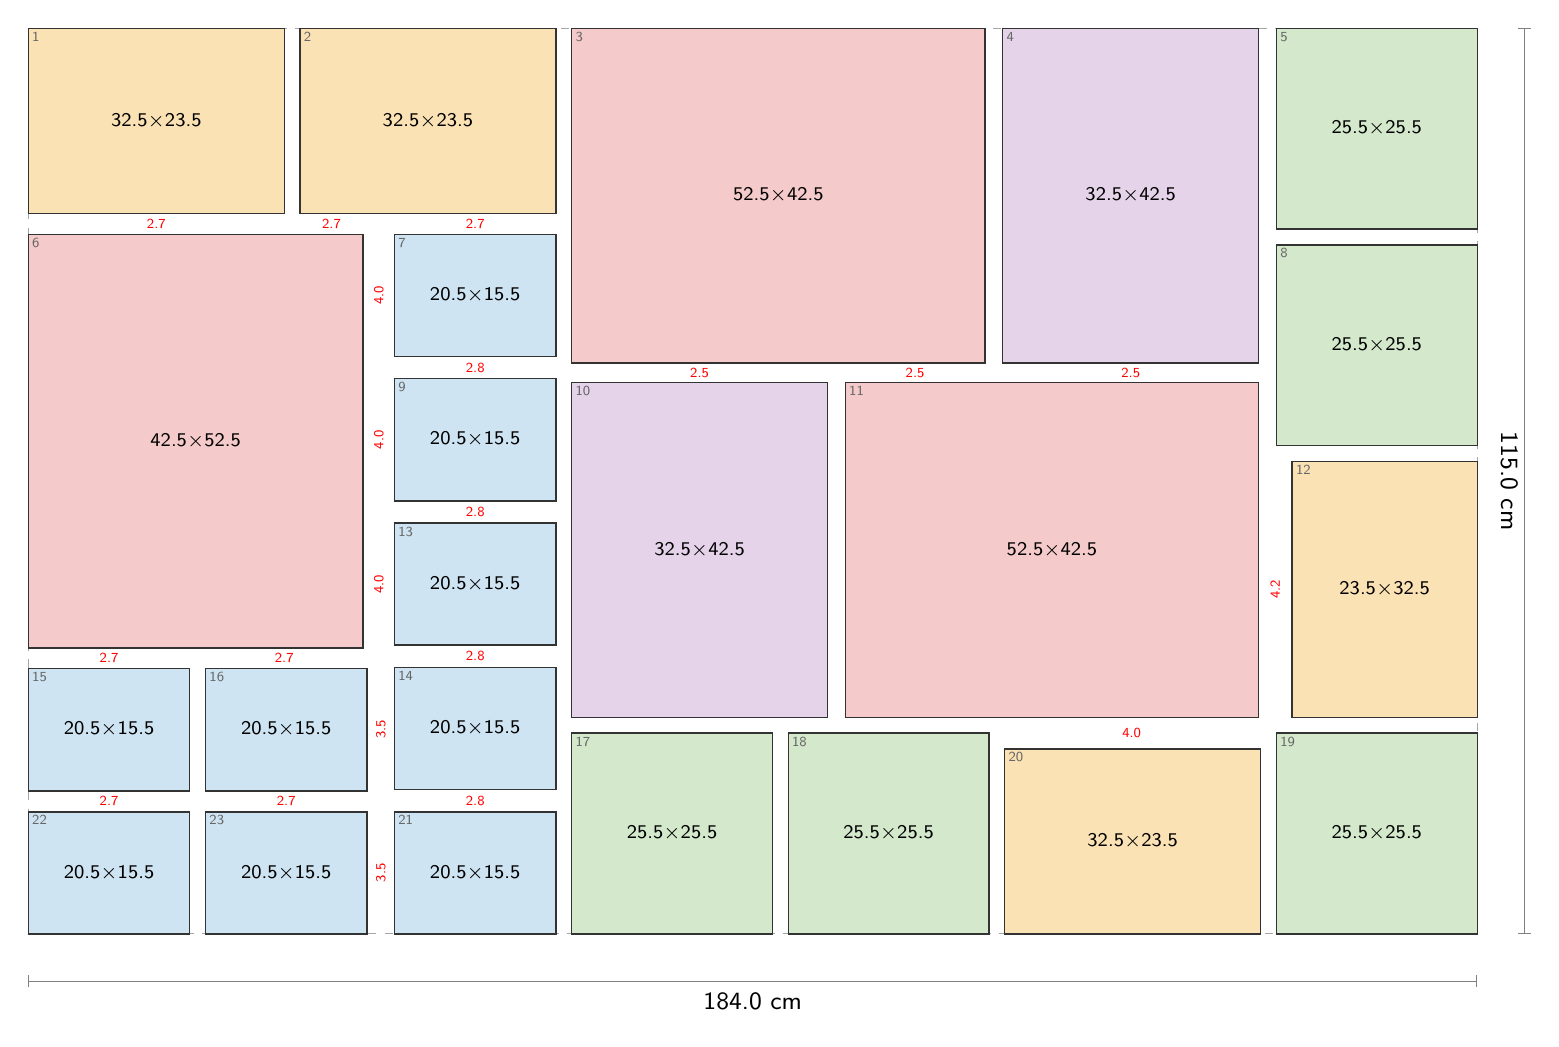
\begin{tikzpicture}[x=1mm, y=-1mm]
\draw[gray!70, dashed, line width=0.4pt] (0,0) rectangle (184.00,115.00);
\filldraw[fill=ft1, draw=black!80, line width=0.5pt] (0.00,0.00) rectangle (32.50,23.50);
\node[align=center, inner sep=0pt] at (16.25,11.75) {\scriptsize 32.5$\times$23.5};
\node[anchor=north west, inner sep=1.2pt, font=\tiny, text=black!60] at (0.00,0.00) {1};
\filldraw[fill=ft1, draw=black!80, line width=0.5pt] (34.50,0.00) rectangle (67.00,23.50);
\node[align=center, inner sep=0pt] at (50.75,11.75) {\scriptsize 32.5$\times$23.5};
\node[anchor=north west, inner sep=1.2pt, font=\tiny, text=black!60] at (34.50,0.00) {2};
\filldraw[fill=ft4, draw=black!80, line width=0.5pt] (69.00,0.00) rectangle (121.50,42.50);
\node[align=center, inner sep=0pt] at (95.25,21.25) {\scriptsize 52.5$\times$42.5};
\node[anchor=north west, inner sep=1.2pt, font=\tiny, text=black!60] at (69.00,0.00) {3};
\filldraw[fill=ft3, draw=black!80, line width=0.5pt] (123.75,0.00) rectangle (156.25,42.50);
\node[align=center, inner sep=0pt] at (140.00,21.25) {\scriptsize 32.5$\times$42.5};
\node[anchor=north west, inner sep=1.2pt, font=\tiny, text=black!60] at (123.75,0.00) {4};
\filldraw[fill=ft2, draw=black!80, line width=0.5pt] (158.50,0.00) rectangle (184.00,25.50);
\node[align=center, inner sep=0pt] at (171.25,12.75) {\scriptsize 25.5$\times$25.5};
\node[anchor=north west, inner sep=1.2pt, font=\tiny, text=black!60] at (158.50,0.00) {5};
\filldraw[fill=ft4, draw=black!80, line width=0.5pt] (0.00,26.17) rectangle (42.50,78.67);
\node[align=center, inner sep=0pt] at (21.25,52.42) {\scriptsize 42.5$\times$52.5};
\node[anchor=north west, inner sep=1.2pt, font=\tiny, text=black!60] at (0.00,26.17) {6};
\filldraw[fill=ft0, draw=black!80, line width=0.5pt] (46.50,26.17) rectangle (67.00,41.67);
\node[align=center, inner sep=0pt] at (56.75,33.92) {\scriptsize 20.5$\times$15.5};
\node[anchor=north west, inner sep=1.2pt, font=\tiny, text=black!60] at (46.50,26.17) {7};
\filldraw[fill=ft2, draw=black!80, line width=0.5pt] (158.50,27.50) rectangle (184.00,53.00);
\node[align=center, inner sep=0pt] at (171.25,40.25) {\scriptsize 25.5$\times$25.5};
\node[anchor=north west, inner sep=1.2pt, font=\tiny, text=black!60] at (158.50,27.50) {8};
\filldraw[fill=ft0, draw=black!80, line width=0.5pt] (46.50,44.50) rectangle (67.00,60.00);
\node[align=center, inner sep=0pt] at (56.75,52.25) {\scriptsize 20.5$\times$15.5};
\node[anchor=north west, inner sep=1.2pt, font=\tiny, text=black!60] at (46.50,44.50) {9};
\filldraw[fill=ft3, draw=black!80, line width=0.5pt] (69.00,45.00) rectangle (101.50,87.50);
\node[align=center, inner sep=0pt] at (85.25,66.25) {\scriptsize 32.5$\times$42.5};
\node[anchor=north west, inner sep=1.2pt, font=\tiny, text=black!60] at (69.00,45.00) {10};
\filldraw[fill=ft4, draw=black!80, line width=0.5pt] (103.75,45.00) rectangle (156.25,87.50);
\node[align=center, inner sep=0pt] at (130.00,66.25) {\scriptsize 52.5$\times$42.5};
\node[anchor=north west, inner sep=1.2pt, font=\tiny, text=black!60] at (103.75,45.00) {11};
\filldraw[fill=ft1, draw=black!80, line width=0.5pt] (160.50,55.00) rectangle (184.00,87.50);
\node[align=center, inner sep=0pt] at (172.25,71.25) {\scriptsize 23.5$\times$32.5};
\node[anchor=north west, inner sep=1.2pt, font=\tiny, text=black!60] at (160.50,55.00) {12};
\filldraw[fill=ft0, draw=black!80, line width=0.5pt] (46.50,62.83) rectangle (67.00,78.33);
\node[align=center, inner sep=0pt] at (56.75,70.58) {\scriptsize 20.5$\times$15.5};
\node[anchor=north west, inner sep=1.2pt, font=\tiny, text=black!60] at (46.50,62.83) {13};
\filldraw[fill=ft0, draw=black!80, line width=0.5pt] (46.50,81.17) rectangle (67.00,96.67);
\node[align=center, inner sep=0pt] at (56.75,88.92) {\scriptsize 20.5$\times$15.5};
\node[anchor=north west, inner sep=1.2pt, font=\tiny, text=black!60] at (46.50,81.17) {14};
\filldraw[fill=ft0, draw=black!80, line width=0.5pt] (0.00,81.33) rectangle (20.50,96.83);
\node[align=center, inner sep=0pt] at (10.25,89.08) {\scriptsize 20.5$\times$15.5};
\node[anchor=north west, inner sep=1.2pt, font=\tiny, text=black!60] at (0.00,81.33) {15};
\filldraw[fill=ft0, draw=black!80, line width=0.5pt] (22.50,81.33) rectangle (43.00,96.83);
\node[align=center, inner sep=0pt] at (32.75,89.08) {\scriptsize 20.5$\times$15.5};
\node[anchor=north west, inner sep=1.2pt, font=\tiny, text=black!60] at (22.50,81.33) {16};
\filldraw[fill=ft2, draw=black!80, line width=0.5pt] (69.00,89.50) rectangle (94.50,115.00);
\node[align=center, inner sep=0pt] at (81.75,102.25) {\scriptsize 25.5$\times$25.5};
\node[anchor=north west, inner sep=1.2pt, font=\tiny, text=black!60] at (69.00,89.50) {17};
\filldraw[fill=ft2, draw=black!80, line width=0.5pt] (96.50,89.50) rectangle (122.00,115.00);
\node[align=center, inner sep=0pt] at (109.25,102.25) {\scriptsize 25.5$\times$25.5};
\node[anchor=north west, inner sep=1.2pt, font=\tiny, text=black!60] at (96.50,89.50) {18};
\filldraw[fill=ft2, draw=black!80, line width=0.5pt] (158.50,89.50) rectangle (184.00,115.00);
\node[align=center, inner sep=0pt] at (171.25,102.25) {\scriptsize 25.5$\times$25.5};
\node[anchor=north west, inner sep=1.2pt, font=\tiny, text=black!60] at (158.50,89.50) {19};
\filldraw[fill=ft1, draw=black!80, line width=0.5pt] (124.00,91.50) rectangle (156.50,115.00);
\node[align=center, inner sep=0pt] at (140.25,103.25) {\scriptsize 32.5$\times$23.5};
\node[anchor=north west, inner sep=1.2pt, font=\tiny, text=black!60] at (124.00,91.50) {20};
\filldraw[fill=ft0, draw=black!80, line width=0.5pt] (46.50,99.50) rectangle (67.00,115.00);
\node[align=center, inner sep=0pt] at (56.75,107.25) {\scriptsize 20.5$\times$15.5};
\node[anchor=north west, inner sep=1.2pt, font=\tiny, text=black!60] at (46.50,99.50) {21};
\filldraw[fill=ft0, draw=black!80, line width=0.5pt] (0.00,99.50) rectangle (20.50,115.00);
\node[align=center, inner sep=0pt] at (10.25,107.25) {\scriptsize 20.5$\times$15.5};
\node[anchor=north west, inner sep=1.2pt, font=\tiny, text=black!60] at (0.00,99.50) {22};
\filldraw[fill=ft0, draw=black!80, line width=0.5pt] (22.50,99.50) rectangle (43.00,115.00);
\node[align=center, inner sep=0pt] at (32.75,107.25) {\scriptsize 20.5$\times$15.5};
\node[anchor=north west, inner sep=1.2pt, font=\tiny, text=black!60] at (22.50,99.50) {23};
\node[font=\tiny, text=red, fill=white, inner sep=0.3pt] at (16.25,24.83) {2.7};
\node[font=\tiny, text=red, fill=white, inner sep=0.3pt] at (38.50,24.83) {2.7};
\node[font=\tiny, text=red, fill=white, inner sep=0.3pt] at (56.75,24.83) {2.7};
\node[font=\tiny, text=red, fill=white, inner sep=0.3pt] at (85.25,43.75) {2.5};
\node[font=\tiny, text=red, fill=white, inner sep=0.3pt] at (112.62,43.75) {2.5};
\node[font=\tiny, text=red, fill=white, inner sep=0.3pt] at (140.00,43.75) {2.5};
\node[font=\tiny, text=red, fill=white, inner sep=0.3pt, rotate=90] at (44.50,33.92) {4.0};
\node[font=\tiny, text=red, fill=white, inner sep=0.3pt, rotate=90] at (44.50,52.25) {4.0};
\node[font=\tiny, text=red, fill=white, inner sep=0.3pt, rotate=90] at (44.50,70.58) {4.0};
\node[font=\tiny, text=red, fill=white, inner sep=0.3pt] at (10.25,80.00) {2.7};
\node[font=\tiny, text=red, fill=white, inner sep=0.3pt] at (32.50,80.00) {2.7};
\node[font=\tiny, text=red, fill=white, inner sep=0.3pt] at (56.75,43.08) {2.8};
\node[font=\tiny, text=red, fill=white, inner sep=0.3pt] at (56.75,61.42) {2.8};
\node[font=\tiny, text=red, fill=white, inner sep=0.3pt, rotate=90] at (158.38,71.25) {4.2};
\node[font=\tiny, text=red, fill=white, inner sep=0.3pt] at (140.12,89.50) {4.0};
\node[font=\tiny, text=red, fill=white, inner sep=0.3pt] at (56.75,79.75) {2.8};
\node[font=\tiny, text=red, fill=white, inner sep=0.3pt] at (56.75,98.08) {2.8};
\node[font=\tiny, text=red, fill=white, inner sep=0.3pt] at (10.25,98.17) {2.7};
\node[font=\tiny, text=red, fill=white, inner sep=0.3pt, rotate=90] at (44.75,89.00) {3.5};
\node[font=\tiny, text=red, fill=white, inner sep=0.3pt] at (32.75,98.17) {2.7};
\node[font=\tiny, text=red, fill=white, inner sep=0.3pt, rotate=90] at (44.75,107.25) {3.5};
\draw[Bar-Bar, gray] (0,121.00) -- (184.00,121.00) node[midway, below=1pt, font=\small, text=black] {184.0 cm};
\draw[Bar-Bar, gray] (190.00,0) -- (190.00,115.00) node[midway, right=1pt, font=\small, text=black, rotate=-90, anchor=north] {115.0 cm};
\end{tikzpicture}\\[4pt]
{\scriptsize Scale 1:10 (1 mm = 1 cm). Red numbers mark gaps that deviate from the nominal gap by more than 0.25 cm. Small grey numbers index the coordinate table.}
\end{minipage}\hfill
\begin{minipage}[t]{0.25\textwidth}\vspace{0pt}
\small
\begin{tabular}{@{}l l@{}}
\toprule
Outer size & 184.0 $\times$ 115.0 cm \\
Nominal gap & 2 cm \\
Actual gaps & 2.0 -- 4.2 cm \\
Max.\ deviation & 2.2 cm \\
Mean deviation & 0.53 cm \\
Border notches & bottom 4 cm \\
Corners filled & 4 / 4 \\
Frames used & 23 of 28 \\
Large frames & {\scriptsize 3, touching 1$\times$ (18 cm), min.\ dist.\ 57 cm} \\
Entropy & 0.68 \\
\quad {\scriptsize mix / variety} & {\scriptsize 0.76 / 0.68} \\
\quad {\scriptsize stagger / lines} & {\scriptsize 0.51 / 0.75 (2 through)} \\
\bottomrule
\end{tabular}

\vspace{8pt}
\scriptsize
\begin{tabular}{@{}c l l r r@{}}
\toprule
 & outer w $\times$ h (cm) &  & used & have \\
\midrule
\tikz[baseline=-0.6ex]\fill[ft0,draw=black!60] (0,0) rectangle (1.2ex,1.2ex); & 20.5$\times$15.5 & L & 9 & 9 \\
\tikz[baseline=-0.6ex]\fill[ft0,draw=black!60] (0,0) rectangle (1.2ex,1.2ex); & 15.5$\times$20.5 & P & 0 & 2 \\
\tikz[baseline=-0.6ex]\fill[ft3,draw=black!60] (0,0) rectangle (1.2ex,1.2ex); & 32.5$\times$42.5 & P & 2 & 2 \\
\tikz[baseline=-0.6ex]\fill[ft3,draw=black!60] (0,0) rectangle (1.2ex,1.2ex); & 42.5$\times$32.5 & L & 0 & 1 \\
\tikz[baseline=-0.6ex]\fill[ft1,draw=black!60] (0,0) rectangle (1.2ex,1.2ex); & 32.5$\times$23.5 & L & 3 & 5 \\
\tikz[baseline=-0.6ex]\fill[ft1,draw=black!60] (0,0) rectangle (1.2ex,1.2ex); & 23.5$\times$32.5 & P & 1 & 1 \\
\tikz[baseline=-0.6ex]\fill[ft2,draw=black!60] (0,0) rectangle (1.2ex,1.2ex); & 25.5$\times$25.5 &  & 5 & 5 \\
\tikz[baseline=-0.6ex]\fill[ft4,draw=black!60] (0,0) rectangle (1.2ex,1.2ex); & 42.5$\times$52.5 & P & 1 & 1 \\
\tikz[baseline=-0.6ex]\fill[ft4,draw=black!60] (0,0) rectangle (1.2ex,1.2ex); & 52.5$\times$42.5 & L & 2 & 2 \\
\bottomrule
\end{tabular}

\vspace{8pt}
{\bfseries Positions} (top-left corner, cm)\\[2pt]
\tiny
\begin{tabular}{@{}r l r r@{}}
\toprule
\# & frame w $\times$ h & x & y \\
\midrule
1 & 32.5 $\times$ 23.5 & 0.0 & 0.0 \\
2 & 32.5 $\times$ 23.5 & 34.5 & 0.0 \\
3 & 52.5 $\times$ 42.5 & 69.0 & 0.0 \\
4 & 32.5 $\times$ 42.5 & 123.8 & 0.0 \\
5 & 25.5 $\times$ 25.5 & 158.5 & 0.0 \\
6 & 42.5 $\times$ 52.5 & 0.0 & 26.2 \\
7 & 20.5 $\times$ 15.5 & 46.5 & 26.2 \\
8 & 25.5 $\times$ 25.5 & 158.5 & 27.5 \\
9 & 20.5 $\times$ 15.5 & 46.5 & 44.5 \\
10 & 32.5 $\times$ 42.5 & 69.0 & 45.0 \\
11 & 52.5 $\times$ 42.5 & 103.8 & 45.0 \\
12 & 23.5 $\times$ 32.5 & 160.5 & 55.0 \\
13 & 20.5 $\times$ 15.5 & 46.5 & 62.8 \\
14 & 20.5 $\times$ 15.5 & 46.5 & 81.2 \\
15 & 20.5 $\times$ 15.5 & 0.0 & 81.3 \\
16 & 20.5 $\times$ 15.5 & 22.5 & 81.3 \\
17 & 25.5 $\times$ 25.5 & 69.0 & 89.5 \\
18 & 25.5 $\times$ 25.5 & 96.5 & 89.5 \\
19 & 25.5 $\times$ 25.5 & 158.5 & 89.5 \\
20 & 32.5 $\times$ 23.5 & 124.0 & 91.5 \\
21 & 20.5 $\times$ 15.5 & 46.5 & 99.5 \\
22 & 20.5 $\times$ 15.5 & 0.0 & 99.5 \\
23 & 20.5 $\times$ 15.5 & 22.5 & 99.5 \\
\bottomrule
\end{tabular}
\end{minipage}
\clearpage

\phantomsection\addcontentsline{toc}{subsection}{Layout 10: 180.0 \texorpdfstring{$\times$}{x} 117.0 cm, 23 frames, gap 4 cm, max.\ deviation 3.0 cm}
\label{lay:free-gap:10}
\begin{minipage}[t]{0.74\textwidth}\vspace{0pt}
{\LARGE\bfseries Layout 10}\hspace{1.5em}{\large 180.0 $\times$ 117.0 cm \quad gap 4 cm \quad 23 frames}\\[8pt]
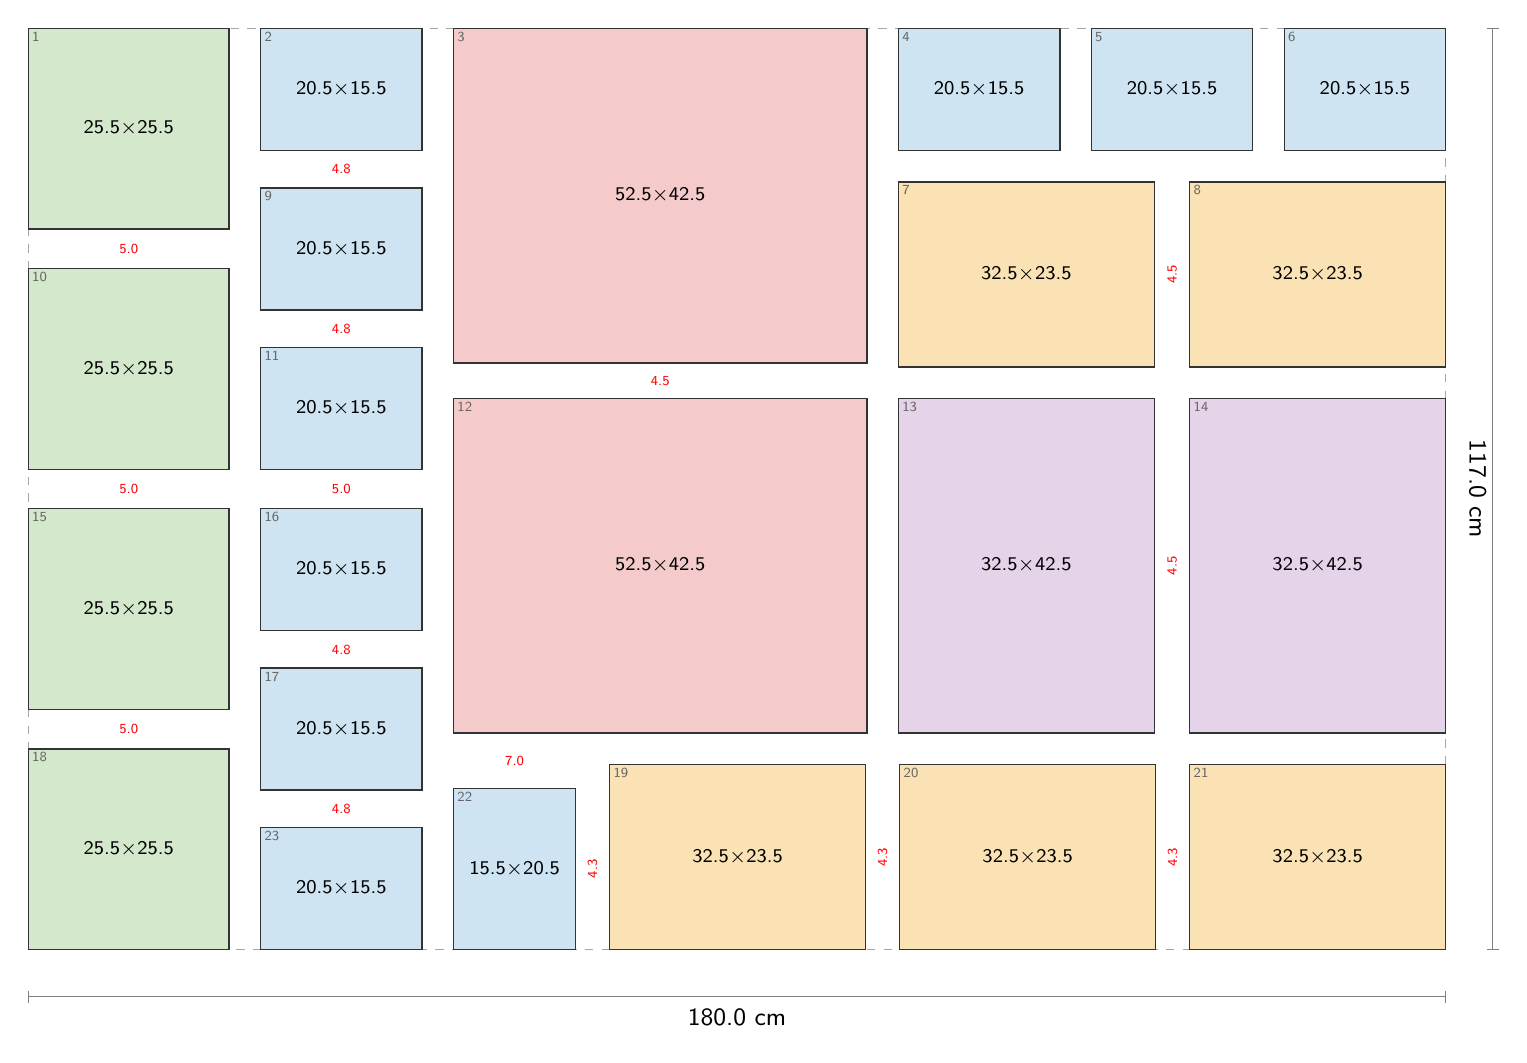
\begin{tikzpicture}[x=1mm, y=-1mm]
\draw[gray!70, dashed, line width=0.4pt] (0,0) rectangle (180.00,117.00);
\filldraw[fill=ft2, draw=black!80, line width=0.5pt] (0.00,0.00) rectangle (25.50,25.50);
\node[align=center, inner sep=0pt] at (12.75,12.75) {\scriptsize 25.5$\times$25.5};
\node[anchor=north west, inner sep=1.2pt, font=\tiny, text=black!60] at (0.00,0.00) {1};
\filldraw[fill=ft0, draw=black!80, line width=0.5pt] (29.50,0.00) rectangle (50.00,15.50);
\node[align=center, inner sep=0pt] at (39.75,7.75) {\scriptsize 20.5$\times$15.5};
\node[anchor=north west, inner sep=1.2pt, font=\tiny, text=black!60] at (29.50,0.00) {2};
\filldraw[fill=ft4, draw=black!80, line width=0.5pt] (54.00,0.00) rectangle (106.50,42.50);
\node[align=center, inner sep=0pt] at (80.25,21.25) {\scriptsize 52.5$\times$42.5};
\node[anchor=north west, inner sep=1.2pt, font=\tiny, text=black!60] at (54.00,0.00) {3};
\filldraw[fill=ft0, draw=black!80, line width=0.5pt] (110.50,0.00) rectangle (131.00,15.50);
\node[align=center, inner sep=0pt] at (120.75,7.75) {\scriptsize 20.5$\times$15.5};
\node[anchor=north west, inner sep=1.2pt, font=\tiny, text=black!60] at (110.50,0.00) {4};
\filldraw[fill=ft0, draw=black!80, line width=0.5pt] (135.00,0.00) rectangle (155.50,15.50);
\node[align=center, inner sep=0pt] at (145.25,7.75) {\scriptsize 20.5$\times$15.5};
\node[anchor=north west, inner sep=1.2pt, font=\tiny, text=black!60] at (135.00,0.00) {5};
\filldraw[fill=ft0, draw=black!80, line width=0.5pt] (159.50,0.00) rectangle (180.00,15.50);
\node[align=center, inner sep=0pt] at (169.75,7.75) {\scriptsize 20.5$\times$15.5};
\node[anchor=north west, inner sep=1.2pt, font=\tiny, text=black!60] at (159.50,0.00) {6};
\filldraw[fill=ft1, draw=black!80, line width=0.5pt] (110.50,19.50) rectangle (143.00,43.00);
\node[align=center, inner sep=0pt] at (126.75,31.25) {\scriptsize 32.5$\times$23.5};
\node[anchor=north west, inner sep=1.2pt, font=\tiny, text=black!60] at (110.50,19.50) {7};
\filldraw[fill=ft1, draw=black!80, line width=0.5pt] (147.50,19.50) rectangle (180.00,43.00);
\node[align=center, inner sep=0pt] at (163.75,31.25) {\scriptsize 32.5$\times$23.5};
\node[anchor=north west, inner sep=1.2pt, font=\tiny, text=black!60] at (147.50,19.50) {8};
\filldraw[fill=ft0, draw=black!80, line width=0.5pt] (29.50,20.25) rectangle (50.00,35.75);
\node[align=center, inner sep=0pt] at (39.75,28.00) {\scriptsize 20.5$\times$15.5};
\node[anchor=north west, inner sep=1.2pt, font=\tiny, text=black!60] at (29.50,20.25) {9};
\filldraw[fill=ft2, draw=black!80, line width=0.5pt] (0.00,30.50) rectangle (25.50,56.00);
\node[align=center, inner sep=0pt] at (12.75,43.25) {\scriptsize 25.5$\times$25.5};
\node[anchor=north west, inner sep=1.2pt, font=\tiny, text=black!60] at (0.00,30.50) {10};
\filldraw[fill=ft0, draw=black!80, line width=0.5pt] (29.50,40.50) rectangle (50.00,56.00);
\node[align=center, inner sep=0pt] at (39.75,48.25) {\scriptsize 20.5$\times$15.5};
\node[anchor=north west, inner sep=1.2pt, font=\tiny, text=black!60] at (29.50,40.50) {11};
\filldraw[fill=ft4, draw=black!80, line width=0.5pt] (54.00,47.00) rectangle (106.50,89.50);
\node[align=center, inner sep=0pt] at (80.25,68.25) {\scriptsize 52.5$\times$42.5};
\node[anchor=north west, inner sep=1.2pt, font=\tiny, text=black!60] at (54.00,47.00) {12};
\filldraw[fill=ft3, draw=black!80, line width=0.5pt] (110.50,47.00) rectangle (143.00,89.50);
\node[align=center, inner sep=0pt] at (126.75,68.25) {\scriptsize 32.5$\times$42.5};
\node[anchor=north west, inner sep=1.2pt, font=\tiny, text=black!60] at (110.50,47.00) {13};
\filldraw[fill=ft3, draw=black!80, line width=0.5pt] (147.50,47.00) rectangle (180.00,89.50);
\node[align=center, inner sep=0pt] at (163.75,68.25) {\scriptsize 32.5$\times$42.5};
\node[anchor=north west, inner sep=1.2pt, font=\tiny, text=black!60] at (147.50,47.00) {14};
\filldraw[fill=ft2, draw=black!80, line width=0.5pt] (0.00,61.00) rectangle (25.50,86.50);
\node[align=center, inner sep=0pt] at (12.75,73.75) {\scriptsize 25.5$\times$25.5};
\node[anchor=north west, inner sep=1.2pt, font=\tiny, text=black!60] at (0.00,61.00) {15};
\filldraw[fill=ft0, draw=black!80, line width=0.5pt] (29.50,61.00) rectangle (50.00,76.50);
\node[align=center, inner sep=0pt] at (39.75,68.75) {\scriptsize 20.5$\times$15.5};
\node[anchor=north west, inner sep=1.2pt, font=\tiny, text=black!60] at (29.50,61.00) {16};
\filldraw[fill=ft0, draw=black!80, line width=0.5pt] (29.50,81.25) rectangle (50.00,96.75);
\node[align=center, inner sep=0pt] at (39.75,89.00) {\scriptsize 20.5$\times$15.5};
\node[anchor=north west, inner sep=1.2pt, font=\tiny, text=black!60] at (29.50,81.25) {17};
\filldraw[fill=ft2, draw=black!80, line width=0.5pt] (0.00,91.50) rectangle (25.50,117.00);
\node[align=center, inner sep=0pt] at (12.75,104.25) {\scriptsize 25.5$\times$25.5};
\node[anchor=north west, inner sep=1.2pt, font=\tiny, text=black!60] at (0.00,91.50) {18};
\filldraw[fill=ft1, draw=black!80, line width=0.5pt] (73.83,93.50) rectangle (106.33,117.00);
\node[align=center, inner sep=0pt] at (90.08,105.25) {\scriptsize 32.5$\times$23.5};
\node[anchor=north west, inner sep=1.2pt, font=\tiny, text=black!60] at (73.83,93.50) {19};
\filldraw[fill=ft1, draw=black!80, line width=0.5pt] (110.67,93.50) rectangle (143.17,117.00);
\node[align=center, inner sep=0pt] at (126.92,105.25) {\scriptsize 32.5$\times$23.5};
\node[anchor=north west, inner sep=1.2pt, font=\tiny, text=black!60] at (110.67,93.50) {20};
\filldraw[fill=ft1, draw=black!80, line width=0.5pt] (147.50,93.50) rectangle (180.00,117.00);
\node[align=center, inner sep=0pt] at (163.75,105.25) {\scriptsize 32.5$\times$23.5};
\node[anchor=north west, inner sep=1.2pt, font=\tiny, text=black!60] at (147.50,93.50) {21};
\filldraw[fill=ft0, draw=black!80, line width=0.5pt] (54.00,96.50) rectangle (69.50,117.00);
\node[align=center, inner sep=0pt] at (61.75,106.75) {\scriptsize 15.5$\times$20.5};
\node[anchor=north west, inner sep=1.2pt, font=\tiny, text=black!60] at (54.00,96.50) {22};
\filldraw[fill=ft0, draw=black!80, line width=0.5pt] (29.50,101.50) rectangle (50.00,117.00);
\node[align=center, inner sep=0pt] at (39.75,109.25) {\scriptsize 20.5$\times$15.5};
\node[anchor=north west, inner sep=1.2pt, font=\tiny, text=black!60] at (29.50,101.50) {23};
\node[font=\tiny, text=red, fill=white, inner sep=0.3pt] at (12.75,28.00) {5.0};
\node[font=\tiny, text=red, fill=white, inner sep=0.3pt] at (39.75,17.88) {4.8};
\node[font=\tiny, text=red, fill=white, inner sep=0.3pt] at (80.25,44.75) {4.5};
\node[font=\tiny, text=red, fill=white, inner sep=0.3pt, rotate=90] at (145.25,31.25) {4.5};
\node[font=\tiny, text=red, fill=white, inner sep=0.3pt] at (39.75,38.12) {4.8};
\node[font=\tiny, text=red, fill=white, inner sep=0.3pt] at (12.75,58.50) {5.0};
\node[font=\tiny, text=red, fill=white, inner sep=0.3pt] at (39.75,58.50) {5.0};
\node[font=\tiny, text=red, fill=white, inner sep=0.3pt] at (61.75,93.00) {7.0};
\node[font=\tiny, text=red, fill=white, inner sep=0.3pt, rotate=90] at (145.25,68.25) {4.5};
\node[font=\tiny, text=red, fill=white, inner sep=0.3pt] at (12.75,89.00) {5.0};
\node[font=\tiny, text=red, fill=white, inner sep=0.3pt] at (39.75,78.88) {4.8};
\node[font=\tiny, text=red, fill=white, inner sep=0.3pt] at (39.75,99.12) {4.8};
\node[font=\tiny, text=red, fill=white, inner sep=0.3pt, rotate=90] at (108.50,105.25) {4.3};
\node[font=\tiny, text=red, fill=white, inner sep=0.3pt, rotate=90] at (145.33,105.25) {4.3};
\node[font=\tiny, text=red, fill=white, inner sep=0.3pt, rotate=90] at (71.67,106.75) {4.3};
\draw[Bar-Bar, gray] (0,123.00) -- (180.00,123.00) node[midway, below=1pt, font=\small, text=black] {180.0 cm};
\draw[Bar-Bar, gray] (186.00,0) -- (186.00,117.00) node[midway, right=1pt, font=\small, text=black, rotate=-90, anchor=north] {117.0 cm};
\end{tikzpicture}\\[4pt]
{\scriptsize Scale 1:10 (1 mm = 1 cm). Red numbers mark gaps that deviate from the nominal gap by more than 0.25 cm. Small grey numbers index the coordinate table.}
\end{minipage}\hfill
\begin{minipage}[t]{0.25\textwidth}\vspace{0pt}
\small
\begin{tabular}{@{}l l@{}}
\toprule
Outer size & 180.0 $\times$ 117.0 cm \\
Nominal gap & 4 cm \\
Actual gaps & 4.0 -- 7.0 cm \\
Max.\ deviation & 3.0 cm \\
Mean deviation & 0.29 cm \\
Border notches & none \\
Corners filled & 4 / 4 \\
Frames used & 23 of 28 \\
Large frames & {\scriptsize 2, touching 1$\times$ (52 cm), min.\ dist.\ 47 cm} \\
Entropy & 0.58 \\
\quad {\scriptsize mix / variety} & {\scriptsize 0.71 / 0.64} \\
\quad {\scriptsize stagger / lines} & {\scriptsize 0.46 / 0.50 (3 through)} \\
\bottomrule
\end{tabular}

\vspace{8pt}
\scriptsize
\begin{tabular}{@{}c l l r r@{}}
\toprule
 & outer w $\times$ h (cm) &  & used & have \\
\midrule
\tikz[baseline=-0.6ex]\fill[ft0,draw=black!60] (0,0) rectangle (1.2ex,1.2ex); & 20.5$\times$15.5 & L & 9 & 9 \\
\tikz[baseline=-0.6ex]\fill[ft0,draw=black!60] (0,0) rectangle (1.2ex,1.2ex); & 15.5$\times$20.5 & P & 1 & 2 \\
\tikz[baseline=-0.6ex]\fill[ft3,draw=black!60] (0,0) rectangle (1.2ex,1.2ex); & 32.5$\times$42.5 & P & 2 & 2 \\
\tikz[baseline=-0.6ex]\fill[ft3,draw=black!60] (0,0) rectangle (1.2ex,1.2ex); & 42.5$\times$32.5 & L & 0 & 1 \\
\tikz[baseline=-0.6ex]\fill[ft1,draw=black!60] (0,0) rectangle (1.2ex,1.2ex); & 32.5$\times$23.5 & L & 5 & 5 \\
\tikz[baseline=-0.6ex]\fill[ft1,draw=black!60] (0,0) rectangle (1.2ex,1.2ex); & 23.5$\times$32.5 & P & 0 & 1 \\
\tikz[baseline=-0.6ex]\fill[ft2,draw=black!60] (0,0) rectangle (1.2ex,1.2ex); & 25.5$\times$25.5 &  & 4 & 5 \\
\tikz[baseline=-0.6ex]\fill[ft4,draw=black!60] (0,0) rectangle (1.2ex,1.2ex); & 42.5$\times$52.5 & P & 0 & 1 \\
\tikz[baseline=-0.6ex]\fill[ft4,draw=black!60] (0,0) rectangle (1.2ex,1.2ex); & 52.5$\times$42.5 & L & 2 & 2 \\
\bottomrule
\end{tabular}

\vspace{8pt}
{\bfseries Positions} (top-left corner, cm)\\[2pt]
\tiny
\begin{tabular}{@{}r l r r@{}}
\toprule
\# & frame w $\times$ h & x & y \\
\midrule
1 & 25.5 $\times$ 25.5 & 0.0 & 0.0 \\
2 & 20.5 $\times$ 15.5 & 29.5 & 0.0 \\
3 & 52.5 $\times$ 42.5 & 54.0 & 0.0 \\
4 & 20.5 $\times$ 15.5 & 110.5 & 0.0 \\
5 & 20.5 $\times$ 15.5 & 135.0 & 0.0 \\
6 & 20.5 $\times$ 15.5 & 159.5 & 0.0 \\
7 & 32.5 $\times$ 23.5 & 110.5 & 19.5 \\
8 & 32.5 $\times$ 23.5 & 147.5 & 19.5 \\
9 & 20.5 $\times$ 15.5 & 29.5 & 20.2 \\
10 & 25.5 $\times$ 25.5 & 0.0 & 30.5 \\
11 & 20.5 $\times$ 15.5 & 29.5 & 40.5 \\
12 & 52.5 $\times$ 42.5 & 54.0 & 47.0 \\
13 & 32.5 $\times$ 42.5 & 110.5 & 47.0 \\
14 & 32.5 $\times$ 42.5 & 147.5 & 47.0 \\
15 & 25.5 $\times$ 25.5 & 0.0 & 61.0 \\
16 & 20.5 $\times$ 15.5 & 29.5 & 61.0 \\
17 & 20.5 $\times$ 15.5 & 29.5 & 81.2 \\
18 & 25.5 $\times$ 25.5 & 0.0 & 91.5 \\
19 & 32.5 $\times$ 23.5 & 73.8 & 93.5 \\
20 & 32.5 $\times$ 23.5 & 110.7 & 93.5 \\
21 & 32.5 $\times$ 23.5 & 147.5 & 93.5 \\
22 & 15.5 $\times$ 20.5 & 54.0 & 96.5 \\
23 & 20.5 $\times$ 15.5 & 29.5 & 101.5 \\
\bottomrule
\end{tabular}
\end{minipage}
\clearpage

\phantomsection\addcontentsline{toc}{subsection}{Layout 11: 182.5 \texorpdfstring{$\times$}{x} 112.5 cm, 22 frames, gap 4.5 cm, max.\ deviation 3.0 cm}
\label{lay:free-gap:11}
\begin{minipage}[t]{0.74\textwidth}\vspace{0pt}
{\LARGE\bfseries Layout 11}\hspace{1.5em}{\large 182.5 $\times$ 112.5 cm \quad gap 4.5 cm \quad 22 frames}\\[8pt]
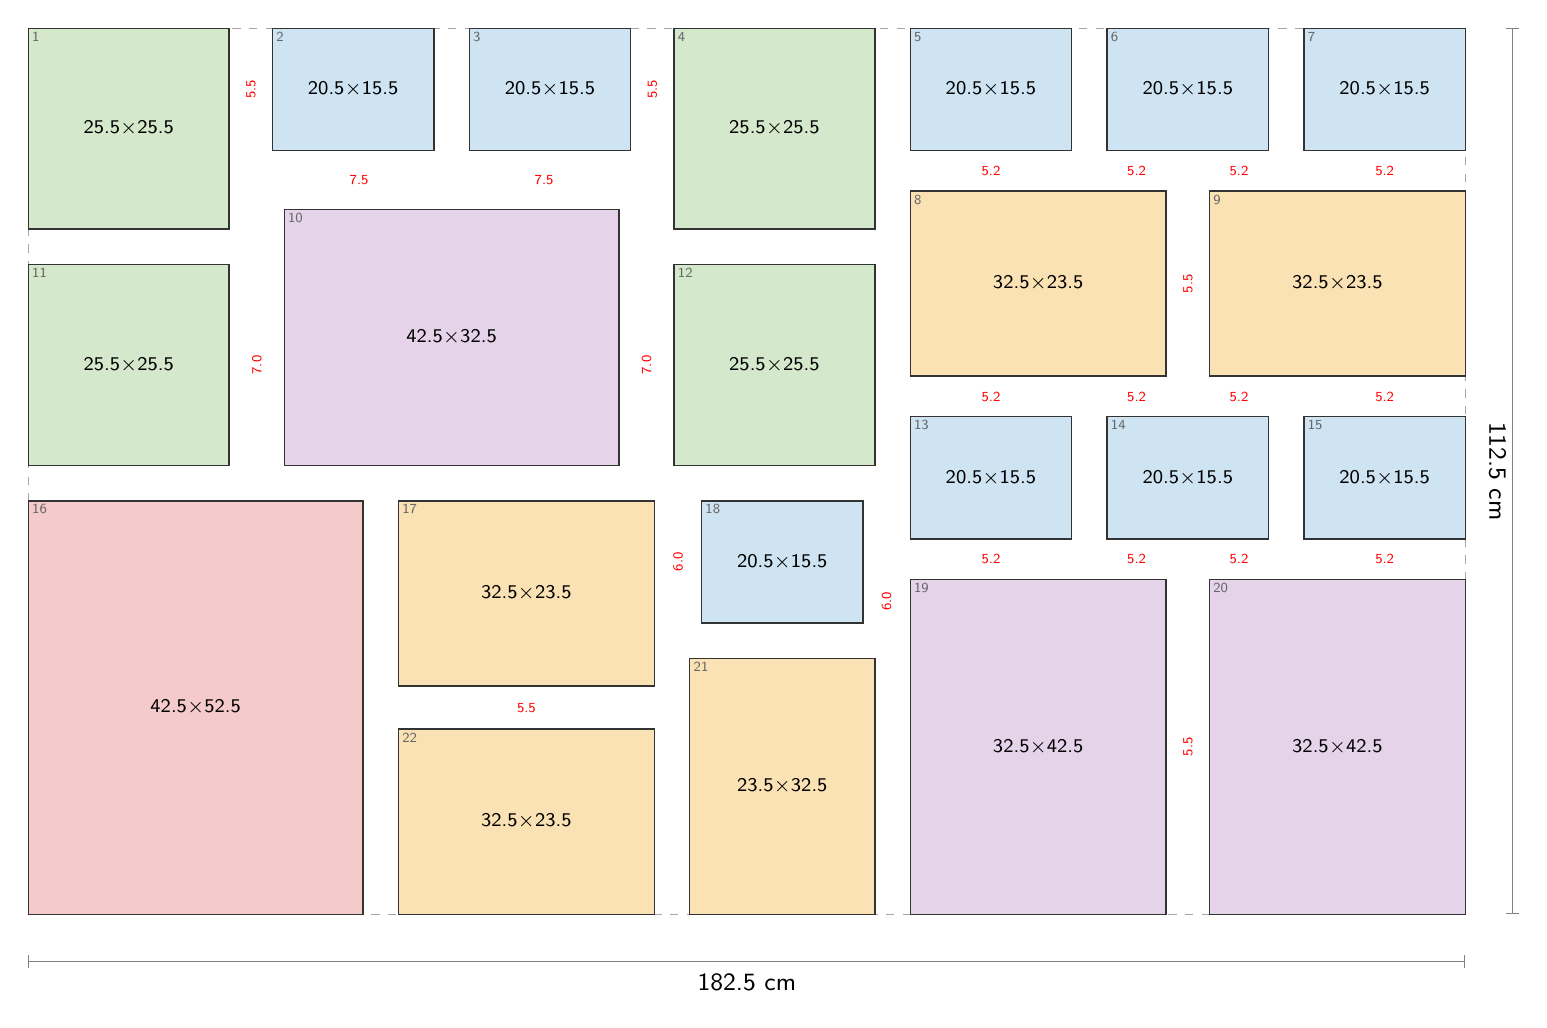
\begin{tikzpicture}[x=1mm, y=-1mm]
\draw[gray!70, dashed, line width=0.4pt] (0,0) rectangle (182.50,112.50);
\filldraw[fill=ft2, draw=black!80, line width=0.5pt] (0.00,0.00) rectangle (25.50,25.50);
\node[align=center, inner sep=0pt] at (12.75,12.75) {\scriptsize 25.5$\times$25.5};
\node[anchor=north west, inner sep=1.2pt, font=\tiny, text=black!60] at (0.00,0.00) {1};
\filldraw[fill=ft0, draw=black!80, line width=0.5pt] (31.00,0.00) rectangle (51.50,15.50);
\node[align=center, inner sep=0pt] at (41.25,7.75) {\scriptsize 20.5$\times$15.5};
\node[anchor=north west, inner sep=1.2pt, font=\tiny, text=black!60] at (31.00,0.00) {2};
\filldraw[fill=ft0, draw=black!80, line width=0.5pt] (56.00,0.00) rectangle (76.50,15.50);
\node[align=center, inner sep=0pt] at (66.25,7.75) {\scriptsize 20.5$\times$15.5};
\node[anchor=north west, inner sep=1.2pt, font=\tiny, text=black!60] at (56.00,0.00) {3};
\filldraw[fill=ft2, draw=black!80, line width=0.5pt] (82.00,0.00) rectangle (107.50,25.50);
\node[align=center, inner sep=0pt] at (94.75,12.75) {\scriptsize 25.5$\times$25.5};
\node[anchor=north west, inner sep=1.2pt, font=\tiny, text=black!60] at (82.00,0.00) {4};
\filldraw[fill=ft0, draw=black!80, line width=0.5pt] (112.00,0.00) rectangle (132.50,15.50);
\node[align=center, inner sep=0pt] at (122.25,7.75) {\scriptsize 20.5$\times$15.5};
\node[anchor=north west, inner sep=1.2pt, font=\tiny, text=black!60] at (112.00,0.00) {5};
\filldraw[fill=ft0, draw=black!80, line width=0.5pt] (137.00,0.00) rectangle (157.50,15.50);
\node[align=center, inner sep=0pt] at (147.25,7.75) {\scriptsize 20.5$\times$15.5};
\node[anchor=north west, inner sep=1.2pt, font=\tiny, text=black!60] at (137.00,0.00) {6};
\filldraw[fill=ft0, draw=black!80, line width=0.5pt] (162.00,0.00) rectangle (182.50,15.50);
\node[align=center, inner sep=0pt] at (172.25,7.75) {\scriptsize 20.5$\times$15.5};
\node[anchor=north west, inner sep=1.2pt, font=\tiny, text=black!60] at (162.00,0.00) {7};
\filldraw[fill=ft1, draw=black!80, line width=0.5pt] (112.00,20.67) rectangle (144.50,44.17);
\node[align=center, inner sep=0pt] at (128.25,32.42) {\scriptsize 32.5$\times$23.5};
\node[anchor=north west, inner sep=1.2pt, font=\tiny, text=black!60] at (112.00,20.67) {8};
\filldraw[fill=ft1, draw=black!80, line width=0.5pt] (150.00,20.67) rectangle (182.50,44.17);
\node[align=center, inner sep=0pt] at (166.25,32.42) {\scriptsize 32.5$\times$23.5};
\node[anchor=north west, inner sep=1.2pt, font=\tiny, text=black!60] at (150.00,20.67) {9};
\filldraw[fill=ft3, draw=black!80, line width=0.5pt] (32.50,23.00) rectangle (75.00,55.50);
\node[align=center, inner sep=0pt] at (53.75,39.25) {\scriptsize 42.5$\times$32.5};
\node[anchor=north west, inner sep=1.2pt, font=\tiny, text=black!60] at (32.50,23.00) {10};
\filldraw[fill=ft2, draw=black!80, line width=0.5pt] (0.00,30.00) rectangle (25.50,55.50);
\node[align=center, inner sep=0pt] at (12.75,42.75) {\scriptsize 25.5$\times$25.5};
\node[anchor=north west, inner sep=1.2pt, font=\tiny, text=black!60] at (0.00,30.00) {11};
\filldraw[fill=ft2, draw=black!80, line width=0.5pt] (82.00,30.00) rectangle (107.50,55.50);
\node[align=center, inner sep=0pt] at (94.75,42.75) {\scriptsize 25.5$\times$25.5};
\node[anchor=north west, inner sep=1.2pt, font=\tiny, text=black!60] at (82.00,30.00) {12};
\filldraw[fill=ft0, draw=black!80, line width=0.5pt] (112.00,49.33) rectangle (132.50,64.83);
\node[align=center, inner sep=0pt] at (122.25,57.08) {\scriptsize 20.5$\times$15.5};
\node[anchor=north west, inner sep=1.2pt, font=\tiny, text=black!60] at (112.00,49.33) {13};
\filldraw[fill=ft0, draw=black!80, line width=0.5pt] (137.00,49.33) rectangle (157.50,64.83);
\node[align=center, inner sep=0pt] at (147.25,57.08) {\scriptsize 20.5$\times$15.5};
\node[anchor=north west, inner sep=1.2pt, font=\tiny, text=black!60] at (137.00,49.33) {14};
\filldraw[fill=ft0, draw=black!80, line width=0.5pt] (162.00,49.33) rectangle (182.50,64.83);
\node[align=center, inner sep=0pt] at (172.25,57.08) {\scriptsize 20.5$\times$15.5};
\node[anchor=north west, inner sep=1.2pt, font=\tiny, text=black!60] at (162.00,49.33) {15};
\filldraw[fill=ft4, draw=black!80, line width=0.5pt] (0.00,60.00) rectangle (42.50,112.50);
\node[align=center, inner sep=0pt] at (21.25,86.25) {\scriptsize 42.5$\times$52.5};
\node[anchor=north west, inner sep=1.2pt, font=\tiny, text=black!60] at (0.00,60.00) {16};
\filldraw[fill=ft1, draw=black!80, line width=0.5pt] (47.00,60.00) rectangle (79.50,83.50);
\node[align=center, inner sep=0pt] at (63.25,71.75) {\scriptsize 32.5$\times$23.5};
\node[anchor=north west, inner sep=1.2pt, font=\tiny, text=black!60] at (47.00,60.00) {17};
\filldraw[fill=ft0, draw=black!80, line width=0.5pt] (85.50,60.00) rectangle (106.00,75.50);
\node[align=center, inner sep=0pt] at (95.75,67.75) {\scriptsize 20.5$\times$15.5};
\node[anchor=north west, inner sep=1.2pt, font=\tiny, text=black!60] at (85.50,60.00) {18};
\filldraw[fill=ft3, draw=black!80, line width=0.5pt] (112.00,70.00) rectangle (144.50,112.50);
\node[align=center, inner sep=0pt] at (128.25,91.25) {\scriptsize 32.5$\times$42.5};
\node[anchor=north west, inner sep=1.2pt, font=\tiny, text=black!60] at (112.00,70.00) {19};
\filldraw[fill=ft3, draw=black!80, line width=0.5pt] (150.00,70.00) rectangle (182.50,112.50);
\node[align=center, inner sep=0pt] at (166.25,91.25) {\scriptsize 32.5$\times$42.5};
\node[anchor=north west, inner sep=1.2pt, font=\tiny, text=black!60] at (150.00,70.00) {20};
\filldraw[fill=ft1, draw=black!80, line width=0.5pt] (84.00,80.00) rectangle (107.50,112.50);
\node[align=center, inner sep=0pt] at (95.75,96.25) {\scriptsize 23.5$\times$32.5};
\node[anchor=north west, inner sep=1.2pt, font=\tiny, text=black!60] at (84.00,80.00) {21};
\filldraw[fill=ft1, draw=black!80, line width=0.5pt] (47.00,89.00) rectangle (79.50,112.50);
\node[align=center, inner sep=0pt] at (63.25,100.75) {\scriptsize 32.5$\times$23.5};
\node[anchor=north west, inner sep=1.2pt, font=\tiny, text=black!60] at (47.00,89.00) {22};
\node[font=\tiny, text=red, fill=white, inner sep=0.3pt, rotate=90] at (28.25,7.75) {5.5};
\node[font=\tiny, text=red, fill=white, inner sep=0.3pt] at (42.00,19.25) {7.5};
\node[font=\tiny, text=red, fill=white, inner sep=0.3pt, rotate=90] at (79.25,7.75) {5.5};
\node[font=\tiny, text=red, fill=white, inner sep=0.3pt] at (65.50,19.25) {7.5};
\node[font=\tiny, text=red, fill=white, inner sep=0.3pt] at (122.25,18.08) {5.2};
\node[font=\tiny, text=red, fill=white, inner sep=0.3pt] at (140.75,18.08) {5.2};
\node[font=\tiny, text=red, fill=white, inner sep=0.3pt] at (153.75,18.08) {5.2};
\node[font=\tiny, text=red, fill=white, inner sep=0.3pt] at (172.25,18.08) {5.2};
\node[font=\tiny, text=red, fill=white, inner sep=0.3pt, rotate=90] at (147.25,32.42) {5.5};
\node[font=\tiny, text=red, fill=white, inner sep=0.3pt] at (122.25,46.75) {5.2};
\node[font=\tiny, text=red, fill=white, inner sep=0.3pt] at (140.75,46.75) {5.2};
\node[font=\tiny, text=red, fill=white, inner sep=0.3pt] at (153.75,46.75) {5.2};
\node[font=\tiny, text=red, fill=white, inner sep=0.3pt] at (172.25,46.75) {5.2};
\node[font=\tiny, text=red, fill=white, inner sep=0.3pt, rotate=90] at (78.50,42.75) {7.0};
\node[font=\tiny, text=red, fill=white, inner sep=0.3pt, rotate=90] at (29.00,42.75) {7.0};
\node[font=\tiny, text=red, fill=white, inner sep=0.3pt] at (122.25,67.42) {5.2};
\node[font=\tiny, text=red, fill=white, inner sep=0.3pt] at (140.75,67.42) {5.2};
\node[font=\tiny, text=red, fill=white, inner sep=0.3pt] at (153.75,67.42) {5.2};
\node[font=\tiny, text=red, fill=white, inner sep=0.3pt] at (172.25,67.42) {5.2};
\node[font=\tiny, text=red, fill=white, inner sep=0.3pt, rotate=90] at (82.50,67.75) {6.0};
\node[font=\tiny, text=red, fill=white, inner sep=0.3pt] at (63.25,86.25) {5.5};
\node[font=\tiny, text=red, fill=white, inner sep=0.3pt, rotate=90] at (109.00,72.75) {6.0};
\node[font=\tiny, text=red, fill=white, inner sep=0.3pt, rotate=90] at (147.25,91.25) {5.5};
\draw[Bar-Bar, gray] (0,118.50) -- (182.50,118.50) node[midway, below=1pt, font=\small, text=black] {182.5 cm};
\draw[Bar-Bar, gray] (188.50,0) -- (188.50,112.50) node[midway, right=1pt, font=\small, text=black, rotate=-90, anchor=north] {112.5 cm};
\end{tikzpicture}\\[4pt]
{\scriptsize Scale 1:10 (1 mm = 1 cm). Red numbers mark gaps that deviate from the nominal gap by more than 0.25 cm. Small grey numbers index the coordinate table.}
\end{minipage}\hfill
\begin{minipage}[t]{0.25\textwidth}\vspace{0pt}
\small
\begin{tabular}{@{}l l@{}}
\toprule
Outer size & 182.5 $\times$ 112.5 cm \\
Nominal gap & 4.5 cm \\
Actual gaps & 4.5 -- 7.5 cm \\
Max.\ deviation & 3.0 cm \\
Mean deviation & 0.64 cm \\
Border notches & none \\
Corners filled & 4 / 4 \\
Frames used & 22 of 28 \\
Large frames & {\scriptsize 1} \\
Entropy & 0.67 \\
\quad {\scriptsize mix / variety} & {\scriptsize 0.74 / 0.72} \\
\quad {\scriptsize stagger / lines} & {\scriptsize 0.47 / 0.75 (2 through)} \\
\bottomrule
\end{tabular}

\vspace{8pt}
\scriptsize
\begin{tabular}{@{}c l l r r@{}}
\toprule
 & outer w $\times$ h (cm) &  & used & have \\
\midrule
\tikz[baseline=-0.6ex]\fill[ft0,draw=black!60] (0,0) rectangle (1.2ex,1.2ex); & 20.5$\times$15.5 & L & 9 & 9 \\
\tikz[baseline=-0.6ex]\fill[ft0,draw=black!60] (0,0) rectangle (1.2ex,1.2ex); & 15.5$\times$20.5 & P & 0 & 2 \\
\tikz[baseline=-0.6ex]\fill[ft3,draw=black!60] (0,0) rectangle (1.2ex,1.2ex); & 32.5$\times$42.5 & P & 2 & 2 \\
\tikz[baseline=-0.6ex]\fill[ft3,draw=black!60] (0,0) rectangle (1.2ex,1.2ex); & 42.5$\times$32.5 & L & 1 & 1 \\
\tikz[baseline=-0.6ex]\fill[ft1,draw=black!60] (0,0) rectangle (1.2ex,1.2ex); & 32.5$\times$23.5 & L & 4 & 5 \\
\tikz[baseline=-0.6ex]\fill[ft1,draw=black!60] (0,0) rectangle (1.2ex,1.2ex); & 23.5$\times$32.5 & P & 1 & 1 \\
\tikz[baseline=-0.6ex]\fill[ft2,draw=black!60] (0,0) rectangle (1.2ex,1.2ex); & 25.5$\times$25.5 &  & 4 & 5 \\
\tikz[baseline=-0.6ex]\fill[ft4,draw=black!60] (0,0) rectangle (1.2ex,1.2ex); & 42.5$\times$52.5 & P & 1 & 1 \\
\tikz[baseline=-0.6ex]\fill[ft4,draw=black!60] (0,0) rectangle (1.2ex,1.2ex); & 52.5$\times$42.5 & L & 0 & 2 \\
\bottomrule
\end{tabular}

\vspace{8pt}
{\bfseries Positions} (top-left corner, cm)\\[2pt]
\tiny
\begin{tabular}{@{}r l r r@{}}
\toprule
\# & frame w $\times$ h & x & y \\
\midrule
1 & 25.5 $\times$ 25.5 & 0.0 & 0.0 \\
2 & 20.5 $\times$ 15.5 & 31.0 & 0.0 \\
3 & 20.5 $\times$ 15.5 & 56.0 & 0.0 \\
4 & 25.5 $\times$ 25.5 & 82.0 & 0.0 \\
5 & 20.5 $\times$ 15.5 & 112.0 & 0.0 \\
6 & 20.5 $\times$ 15.5 & 137.0 & 0.0 \\
7 & 20.5 $\times$ 15.5 & 162.0 & 0.0 \\
8 & 32.5 $\times$ 23.5 & 112.0 & 20.7 \\
9 & 32.5 $\times$ 23.5 & 150.0 & 20.7 \\
10 & 42.5 $\times$ 32.5 & 32.5 & 23.0 \\
11 & 25.5 $\times$ 25.5 & 0.0 & 30.0 \\
12 & 25.5 $\times$ 25.5 & 82.0 & 30.0 \\
13 & 20.5 $\times$ 15.5 & 112.0 & 49.3 \\
14 & 20.5 $\times$ 15.5 & 137.0 & 49.3 \\
15 & 20.5 $\times$ 15.5 & 162.0 & 49.3 \\
16 & 42.5 $\times$ 52.5 & 0.0 & 60.0 \\
17 & 32.5 $\times$ 23.5 & 47.0 & 60.0 \\
18 & 20.5 $\times$ 15.5 & 85.5 & 60.0 \\
19 & 32.5 $\times$ 42.5 & 112.0 & 70.0 \\
20 & 32.5 $\times$ 42.5 & 150.0 & 70.0 \\
21 & 23.5 $\times$ 32.5 & 84.0 & 80.0 \\
22 & 32.5 $\times$ 23.5 & 47.0 & 89.0 \\
\bottomrule
\end{tabular}
\end{minipage}
\clearpage

\phantomsection\addcontentsline{toc}{subsection}{Layout 12: 170.5 \texorpdfstring{$\times$}{x} 114.5 cm, 22 frames, gap 2 cm, max.\ deviation 3.0 cm}
\label{lay:free-gap:12}
\begin{minipage}[t]{0.74\textwidth}\vspace{0pt}
{\LARGE\bfseries Layout 12}\hspace{1.5em}{\large 170.5 $\times$ 114.5 cm \quad gap 2 cm \quad 22 frames}\\[8pt]
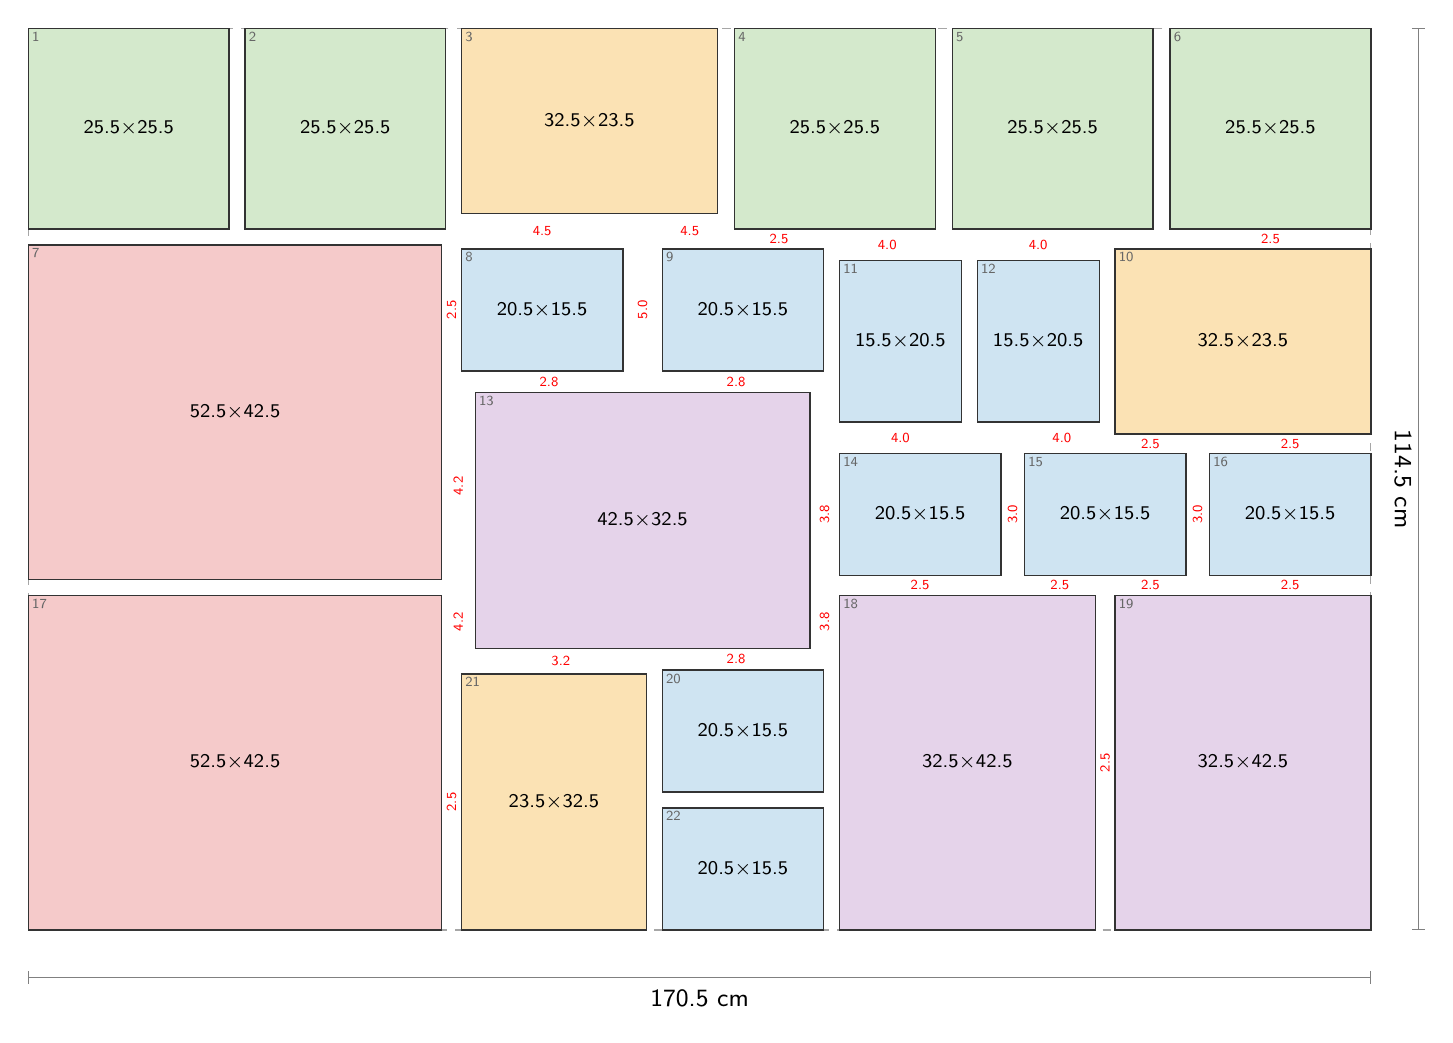
\begin{tikzpicture}[x=1mm, y=-1mm]
\draw[gray!70, dashed, line width=0.4pt] (0,0) rectangle (170.50,114.50);
\filldraw[fill=ft2, draw=black!80, line width=0.5pt] (0.00,0.00) rectangle (25.50,25.50);
\node[align=center, inner sep=0pt] at (12.75,12.75) {\scriptsize 25.5$\times$25.5};
\node[anchor=north west, inner sep=1.2pt, font=\tiny, text=black!60] at (0.00,0.00) {1};
\filldraw[fill=ft2, draw=black!80, line width=0.5pt] (27.50,0.00) rectangle (53.00,25.50);
\node[align=center, inner sep=0pt] at (40.25,12.75) {\scriptsize 25.5$\times$25.5};
\node[anchor=north west, inner sep=1.2pt, font=\tiny, text=black!60] at (27.50,0.00) {2};
\filldraw[fill=ft1, draw=black!80, line width=0.5pt] (55.00,0.00) rectangle (87.50,23.50);
\node[align=center, inner sep=0pt] at (71.25,11.75) {\scriptsize 32.5$\times$23.5};
\node[anchor=north west, inner sep=1.2pt, font=\tiny, text=black!60] at (55.00,0.00) {3};
\filldraw[fill=ft2, draw=black!80, line width=0.5pt] (89.67,0.00) rectangle (115.17,25.50);
\node[align=center, inner sep=0pt] at (102.42,12.75) {\scriptsize 25.5$\times$25.5};
\node[anchor=north west, inner sep=1.2pt, font=\tiny, text=black!60] at (89.67,0.00) {4};
\filldraw[fill=ft2, draw=black!80, line width=0.5pt] (117.33,0.00) rectangle (142.83,25.50);
\node[align=center, inner sep=0pt] at (130.08,12.75) {\scriptsize 25.5$\times$25.5};
\node[anchor=north west, inner sep=1.2pt, font=\tiny, text=black!60] at (117.33,0.00) {5};
\filldraw[fill=ft2, draw=black!80, line width=0.5pt] (145.00,0.00) rectangle (170.50,25.50);
\node[align=center, inner sep=0pt] at (157.75,12.75) {\scriptsize 25.5$\times$25.5};
\node[anchor=north west, inner sep=1.2pt, font=\tiny, text=black!60] at (145.00,0.00) {6};
\filldraw[fill=ft4, draw=black!80, line width=0.5pt] (0.00,27.50) rectangle (52.50,70.00);
\node[align=center, inner sep=0pt] at (26.25,48.75) {\scriptsize 52.5$\times$42.5};
\node[anchor=north west, inner sep=1.2pt, font=\tiny, text=black!60] at (0.00,27.50) {7};
\filldraw[fill=ft0, draw=black!80, line width=0.5pt] (55.00,28.00) rectangle (75.50,43.50);
\node[align=center, inner sep=0pt] at (65.25,35.75) {\scriptsize 20.5$\times$15.5};
\node[anchor=north west, inner sep=1.2pt, font=\tiny, text=black!60] at (55.00,28.00) {8};
\filldraw[fill=ft0, draw=black!80, line width=0.5pt] (80.50,28.00) rectangle (101.00,43.50);
\node[align=center, inner sep=0pt] at (90.75,35.75) {\scriptsize 20.5$\times$15.5};
\node[anchor=north west, inner sep=1.2pt, font=\tiny, text=black!60] at (80.50,28.00) {9};
\filldraw[fill=ft1, draw=black!80, line width=0.5pt] (138.00,28.00) rectangle (170.50,51.50);
\node[align=center, inner sep=0pt] at (154.25,39.75) {\scriptsize 32.5$\times$23.5};
\node[anchor=north west, inner sep=1.2pt, font=\tiny, text=black!60] at (138.00,28.00) {10};
\filldraw[fill=ft0, draw=black!80, line width=0.5pt] (103.00,29.50) rectangle (118.50,50.00);
\node[align=center, inner sep=0pt] at (110.75,39.75) {\scriptsize 15.5$\times$20.5};
\node[anchor=north west, inner sep=1.2pt, font=\tiny, text=black!60] at (103.00,29.50) {11};
\filldraw[fill=ft0, draw=black!80, line width=0.5pt] (120.50,29.50) rectangle (136.00,50.00);
\node[align=center, inner sep=0pt] at (128.25,39.75) {\scriptsize 15.5$\times$20.5};
\node[anchor=north west, inner sep=1.2pt, font=\tiny, text=black!60] at (120.50,29.50) {12};
\filldraw[fill=ft3, draw=black!80, line width=0.5pt] (56.75,46.25) rectangle (99.25,78.75);
\node[align=center, inner sep=0pt] at (78.00,62.50) {\scriptsize 42.5$\times$32.5};
\node[anchor=north west, inner sep=1.2pt, font=\tiny, text=black!60] at (56.75,46.25) {13};
\filldraw[fill=ft0, draw=black!80, line width=0.5pt] (103.00,54.00) rectangle (123.50,69.50);
\node[align=center, inner sep=0pt] at (113.25,61.75) {\scriptsize 20.5$\times$15.5};
\node[anchor=north west, inner sep=1.2pt, font=\tiny, text=black!60] at (103.00,54.00) {14};
\filldraw[fill=ft0, draw=black!80, line width=0.5pt] (126.50,54.00) rectangle (147.00,69.50);
\node[align=center, inner sep=0pt] at (136.75,61.75) {\scriptsize 20.5$\times$15.5};
\node[anchor=north west, inner sep=1.2pt, font=\tiny, text=black!60] at (126.50,54.00) {15};
\filldraw[fill=ft0, draw=black!80, line width=0.5pt] (150.00,54.00) rectangle (170.50,69.50);
\node[align=center, inner sep=0pt] at (160.25,61.75) {\scriptsize 20.5$\times$15.5};
\node[anchor=north west, inner sep=1.2pt, font=\tiny, text=black!60] at (150.00,54.00) {16};
\filldraw[fill=ft4, draw=black!80, line width=0.5pt] (0.00,72.00) rectangle (52.50,114.50);
\node[align=center, inner sep=0pt] at (26.25,93.25) {\scriptsize 52.5$\times$42.5};
\node[anchor=north west, inner sep=1.2pt, font=\tiny, text=black!60] at (0.00,72.00) {17};
\filldraw[fill=ft3, draw=black!80, line width=0.5pt] (103.00,72.00) rectangle (135.50,114.50);
\node[align=center, inner sep=0pt] at (119.25,93.25) {\scriptsize 32.5$\times$42.5};
\node[anchor=north west, inner sep=1.2pt, font=\tiny, text=black!60] at (103.00,72.00) {18};
\filldraw[fill=ft3, draw=black!80, line width=0.5pt] (138.00,72.00) rectangle (170.50,114.50);
\node[align=center, inner sep=0pt] at (154.25,93.25) {\scriptsize 32.5$\times$42.5};
\node[anchor=north west, inner sep=1.2pt, font=\tiny, text=black!60] at (138.00,72.00) {19};
\filldraw[fill=ft0, draw=black!80, line width=0.5pt] (80.50,81.50) rectangle (101.00,97.00);
\node[align=center, inner sep=0pt] at (90.75,89.25) {\scriptsize 20.5$\times$15.5};
\node[anchor=north west, inner sep=1.2pt, font=\tiny, text=black!60] at (80.50,81.50) {20};
\filldraw[fill=ft1, draw=black!80, line width=0.5pt] (55.00,82.00) rectangle (78.50,114.50);
\node[align=center, inner sep=0pt] at (66.75,98.25) {\scriptsize 23.5$\times$32.5};
\node[anchor=north west, inner sep=1.2pt, font=\tiny, text=black!60] at (55.00,82.00) {21};
\filldraw[fill=ft0, draw=black!80, line width=0.5pt] (80.50,99.00) rectangle (101.00,114.50);
\node[align=center, inner sep=0pt] at (90.75,106.75) {\scriptsize 20.5$\times$15.5};
\node[anchor=north west, inner sep=1.2pt, font=\tiny, text=black!60] at (80.50,99.00) {22};
\node[font=\tiny, text=red, fill=white, inner sep=0.3pt] at (65.25,25.75) {4.5};
\node[font=\tiny, text=red, fill=white, inner sep=0.3pt] at (84.00,25.75) {4.5};
\node[font=\tiny, text=red, fill=white, inner sep=0.3pt] at (95.33,26.75) {2.5};
\node[font=\tiny, text=red, fill=white, inner sep=0.3pt] at (109.08,27.50) {4.0};
\node[font=\tiny, text=red, fill=white, inner sep=0.3pt] at (128.25,27.50) {4.0};
\node[font=\tiny, text=red, fill=white, inner sep=0.3pt] at (157.75,26.75) {2.5};
\node[font=\tiny, text=red, fill=white, inner sep=0.3pt, rotate=90] at (53.75,35.75) {2.5};
\node[font=\tiny, text=red, fill=white, inner sep=0.3pt, rotate=90] at (54.62,58.12) {4.2};
\node[font=\tiny, text=red, fill=white, inner sep=0.3pt, rotate=90] at (78.00,35.75) {5.0};
\node[font=\tiny, text=red, fill=white, inner sep=0.3pt] at (66.12,44.88) {2.8};
\node[font=\tiny, text=red, fill=white, inner sep=0.3pt] at (89.88,44.88) {2.8};
\node[font=\tiny, text=red, fill=white, inner sep=0.3pt] at (142.50,52.75) {2.5};
\node[font=\tiny, text=red, fill=white, inner sep=0.3pt] at (160.25,52.75) {2.5};
\node[font=\tiny, text=red, fill=white, inner sep=0.3pt] at (110.75,52.00) {4.0};
\node[font=\tiny, text=red, fill=white, inner sep=0.3pt] at (131.25,52.00) {4.0};
\node[font=\tiny, text=red, fill=white, inner sep=0.3pt, rotate=90] at (101.12,61.75) {3.8};
\node[font=\tiny, text=red, fill=white, inner sep=0.3pt, rotate=90] at (101.12,75.38) {3.8};
\node[font=\tiny, text=red, fill=white, inner sep=0.3pt] at (89.88,80.12) {2.8};
\node[font=\tiny, text=red, fill=white, inner sep=0.3pt] at (67.62,80.38) {3.2};
\node[font=\tiny, text=red, fill=white, inner sep=0.3pt, rotate=90] at (125.00,61.75) {3.0};
\node[font=\tiny, text=red, fill=white, inner sep=0.3pt] at (113.25,70.75) {2.5};
\node[font=\tiny, text=red, fill=white, inner sep=0.3pt, rotate=90] at (148.50,61.75) {3.0};
\node[font=\tiny, text=red, fill=white, inner sep=0.3pt] at (131.00,70.75) {2.5};
\node[font=\tiny, text=red, fill=white, inner sep=0.3pt] at (142.50,70.75) {2.5};
\node[font=\tiny, text=red, fill=white, inner sep=0.3pt] at (160.25,70.75) {2.5};
\node[font=\tiny, text=red, fill=white, inner sep=0.3pt, rotate=90] at (54.62,75.38) {4.2};
\node[font=\tiny, text=red, fill=white, inner sep=0.3pt, rotate=90] at (53.75,98.25) {2.5};
\node[font=\tiny, text=red, fill=white, inner sep=0.3pt, rotate=90] at (136.75,93.25) {2.5};
\draw[Bar-Bar, gray] (0,120.50) -- (170.50,120.50) node[midway, below=1pt, font=\small, text=black] {170.5 cm};
\draw[Bar-Bar, gray] (176.50,0) -- (176.50,114.50) node[midway, right=1pt, font=\small, text=black, rotate=-90, anchor=north] {114.5 cm};
\end{tikzpicture}\\[4pt]
{\scriptsize Scale 1:10 (1 mm = 1 cm). Red numbers mark gaps that deviate from the nominal gap by more than 0.25 cm. Small grey numbers index the coordinate table.}
\end{minipage}\hfill
\begin{minipage}[t]{0.25\textwidth}\vspace{0pt}
\small
\begin{tabular}{@{}l l@{}}
\toprule
Outer size & 170.5 $\times$ 114.5 cm \\
Nominal gap & 2 cm \\
Actual gaps & 2.0 -- 5.0 cm \\
Max.\ deviation & 3.0 cm \\
Mean deviation & 0.81 cm \\
Border notches & none \\
Corners filled & 4 / 4 \\
Frames used & 22 of 28 \\
Large frames & {\scriptsize 2, touching 1$\times$ (52 cm), min.\ dist.\ 44 cm} \\
Entropy & 0.72 \\
\quad {\scriptsize mix / variety} & {\scriptsize 0.84 / 0.72} \\
\quad {\scriptsize stagger / lines} & {\scriptsize 0.56 / 0.75 (2 through)} \\
\bottomrule
\end{tabular}

\vspace{8pt}
\scriptsize
\begin{tabular}{@{}c l l r r@{}}
\toprule
 & outer w $\times$ h (cm) &  & used & have \\
\midrule
\tikz[baseline=-0.6ex]\fill[ft0,draw=black!60] (0,0) rectangle (1.2ex,1.2ex); & 20.5$\times$15.5 & L & 7 & 9 \\
\tikz[baseline=-0.6ex]\fill[ft0,draw=black!60] (0,0) rectangle (1.2ex,1.2ex); & 15.5$\times$20.5 & P & 2 & 2 \\
\tikz[baseline=-0.6ex]\fill[ft3,draw=black!60] (0,0) rectangle (1.2ex,1.2ex); & 32.5$\times$42.5 & P & 2 & 2 \\
\tikz[baseline=-0.6ex]\fill[ft3,draw=black!60] (0,0) rectangle (1.2ex,1.2ex); & 42.5$\times$32.5 & L & 1 & 1 \\
\tikz[baseline=-0.6ex]\fill[ft1,draw=black!60] (0,0) rectangle (1.2ex,1.2ex); & 32.5$\times$23.5 & L & 2 & 5 \\
\tikz[baseline=-0.6ex]\fill[ft1,draw=black!60] (0,0) rectangle (1.2ex,1.2ex); & 23.5$\times$32.5 & P & 1 & 1 \\
\tikz[baseline=-0.6ex]\fill[ft2,draw=black!60] (0,0) rectangle (1.2ex,1.2ex); & 25.5$\times$25.5 &  & 5 & 5 \\
\tikz[baseline=-0.6ex]\fill[ft4,draw=black!60] (0,0) rectangle (1.2ex,1.2ex); & 42.5$\times$52.5 & P & 0 & 1 \\
\tikz[baseline=-0.6ex]\fill[ft4,draw=black!60] (0,0) rectangle (1.2ex,1.2ex); & 52.5$\times$42.5 & L & 2 & 2 \\
\bottomrule
\end{tabular}

\vspace{8pt}
{\bfseries Positions} (top-left corner, cm)\\[2pt]
\tiny
\begin{tabular}{@{}r l r r@{}}
\toprule
\# & frame w $\times$ h & x & y \\
\midrule
1 & 25.5 $\times$ 25.5 & 0.0 & 0.0 \\
2 & 25.5 $\times$ 25.5 & 27.5 & 0.0 \\
3 & 32.5 $\times$ 23.5 & 55.0 & 0.0 \\
4 & 25.5 $\times$ 25.5 & 89.7 & 0.0 \\
5 & 25.5 $\times$ 25.5 & 117.3 & 0.0 \\
6 & 25.5 $\times$ 25.5 & 145.0 & 0.0 \\
7 & 52.5 $\times$ 42.5 & 0.0 & 27.5 \\
8 & 20.5 $\times$ 15.5 & 55.0 & 28.0 \\
9 & 20.5 $\times$ 15.5 & 80.5 & 28.0 \\
10 & 32.5 $\times$ 23.5 & 138.0 & 28.0 \\
11 & 15.5 $\times$ 20.5 & 103.0 & 29.5 \\
12 & 15.5 $\times$ 20.5 & 120.5 & 29.5 \\
13 & 42.5 $\times$ 32.5 & 56.8 & 46.2 \\
14 & 20.5 $\times$ 15.5 & 103.0 & 54.0 \\
15 & 20.5 $\times$ 15.5 & 126.5 & 54.0 \\
16 & 20.5 $\times$ 15.5 & 150.0 & 54.0 \\
17 & 52.5 $\times$ 42.5 & 0.0 & 72.0 \\
18 & 32.5 $\times$ 42.5 & 103.0 & 72.0 \\
19 & 32.5 $\times$ 42.5 & 138.0 & 72.0 \\
20 & 20.5 $\times$ 15.5 & 80.5 & 81.5 \\
21 & 23.5 $\times$ 32.5 & 55.0 & 82.0 \\
22 & 20.5 $\times$ 15.5 & 80.5 & 99.0 \\
\bottomrule
\end{tabular}
\end{minipage}
\clearpage

\phantomsection\addcontentsline{toc}{subsection}{Layout 13: 177.5 \texorpdfstring{$\times$}{x} 113.5 cm, 21 frames, gap 1.5 cm, max.\ deviation 2.0 cm}
\label{lay:free-gap:13}
\begin{minipage}[t]{0.74\textwidth}\vspace{0pt}
{\LARGE\bfseries Layout 13}\hspace{1.5em}{\large 177.5 $\times$ 113.5 cm \quad gap 1.5 cm \quad 21 frames}\\[8pt]
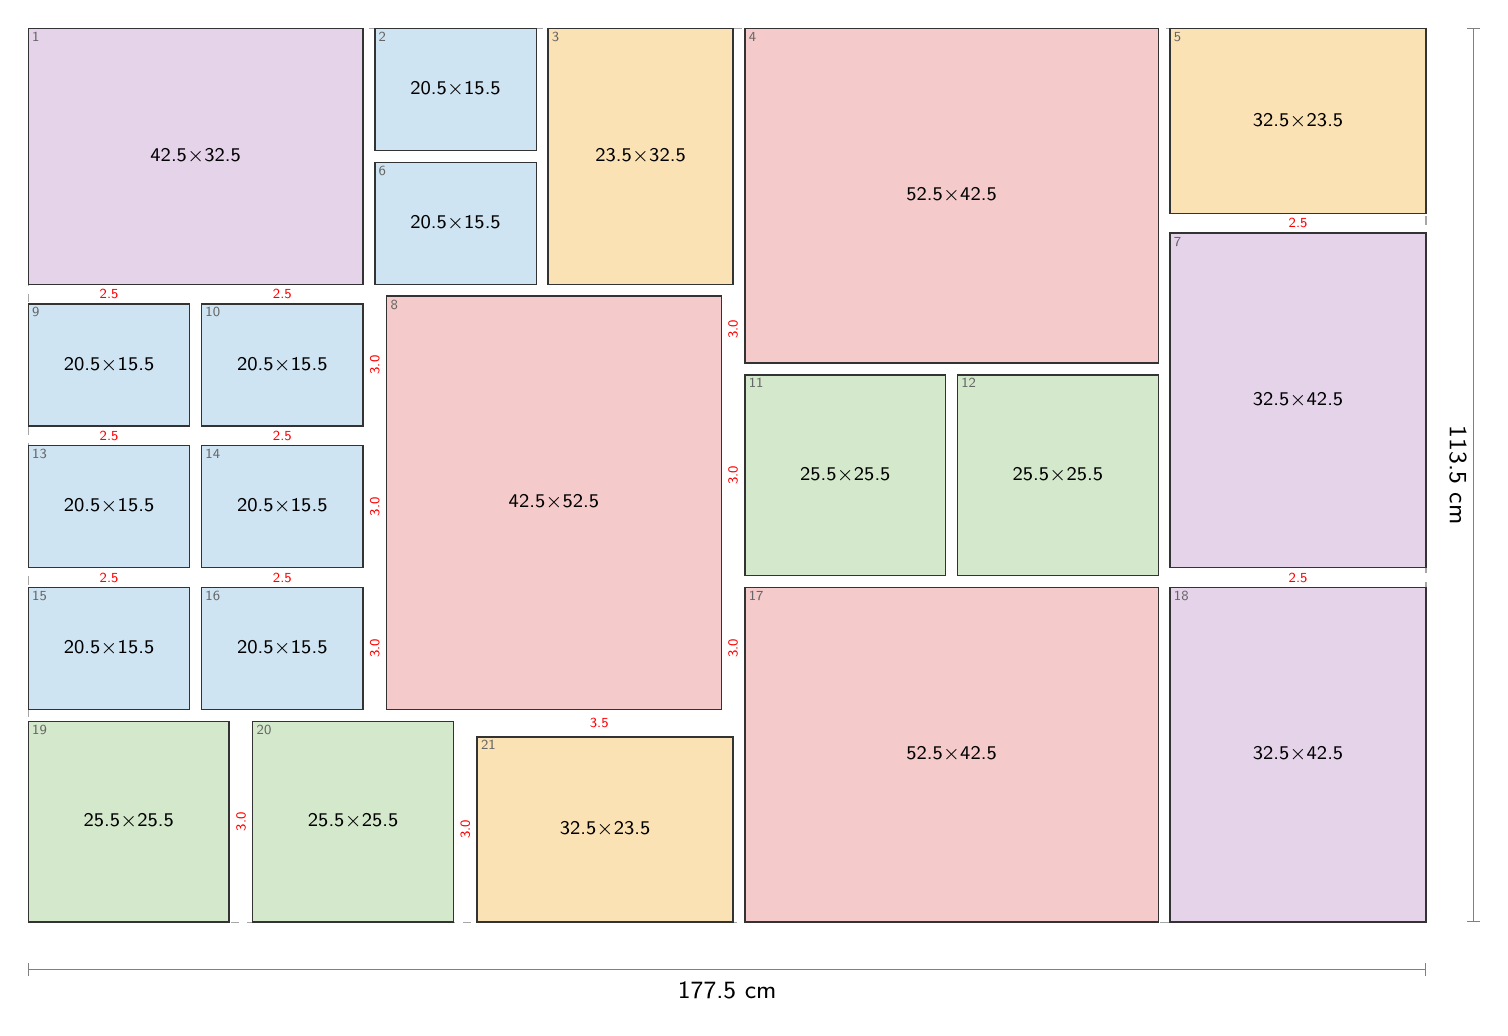
\begin{tikzpicture}[x=1mm, y=-1mm]
\draw[gray!70, dashed, line width=0.4pt] (0,0) rectangle (177.50,113.50);
\filldraw[fill=ft3, draw=black!80, line width=0.5pt] (0.00,0.00) rectangle (42.50,32.50);
\node[align=center, inner sep=0pt] at (21.25,16.25) {\scriptsize 42.5$\times$32.5};
\node[anchor=north west, inner sep=1.2pt, font=\tiny, text=black!60] at (0.00,0.00) {1};
\filldraw[fill=ft0, draw=black!80, line width=0.5pt] (44.00,0.00) rectangle (64.50,15.50);
\node[align=center, inner sep=0pt] at (54.25,7.75) {\scriptsize 20.5$\times$15.5};
\node[anchor=north west, inner sep=1.2pt, font=\tiny, text=black!60] at (44.00,0.00) {2};
\filldraw[fill=ft1, draw=black!80, line width=0.5pt] (66.00,0.00) rectangle (89.50,32.50);
\node[align=center, inner sep=0pt] at (77.75,16.25) {\scriptsize 23.5$\times$32.5};
\node[anchor=north west, inner sep=1.2pt, font=\tiny, text=black!60] at (66.00,0.00) {3};
\filldraw[fill=ft4, draw=black!80, line width=0.5pt] (91.00,0.00) rectangle (143.50,42.50);
\node[align=center, inner sep=0pt] at (117.25,21.25) {\scriptsize 52.5$\times$42.5};
\node[anchor=north west, inner sep=1.2pt, font=\tiny, text=black!60] at (91.00,0.00) {4};
\filldraw[fill=ft1, draw=black!80, line width=0.5pt] (145.00,0.00) rectangle (177.50,23.50);
\node[align=center, inner sep=0pt] at (161.25,11.75) {\scriptsize 32.5$\times$23.5};
\node[anchor=north west, inner sep=1.2pt, font=\tiny, text=black!60] at (145.00,0.00) {5};
\filldraw[fill=ft0, draw=black!80, line width=0.5pt] (44.00,17.00) rectangle (64.50,32.50);
\node[align=center, inner sep=0pt] at (54.25,24.75) {\scriptsize 20.5$\times$15.5};
\node[anchor=north west, inner sep=1.2pt, font=\tiny, text=black!60] at (44.00,17.00) {6};
\filldraw[fill=ft3, draw=black!80, line width=0.5pt] (145.00,26.00) rectangle (177.50,68.50);
\node[align=center, inner sep=0pt] at (161.25,47.25) {\scriptsize 32.5$\times$42.5};
\node[anchor=north west, inner sep=1.2pt, font=\tiny, text=black!60] at (145.00,26.00) {7};
\filldraw[fill=ft4, draw=black!80, line width=0.5pt] (45.50,34.00) rectangle (88.00,86.50);
\node[align=center, inner sep=0pt] at (66.75,60.25) {\scriptsize 42.5$\times$52.5};
\node[anchor=north west, inner sep=1.2pt, font=\tiny, text=black!60] at (45.50,34.00) {8};
\filldraw[fill=ft0, draw=black!80, line width=0.5pt] (0.00,35.00) rectangle (20.50,50.50);
\node[align=center, inner sep=0pt] at (10.25,42.75) {\scriptsize 20.5$\times$15.5};
\node[anchor=north west, inner sep=1.2pt, font=\tiny, text=black!60] at (0.00,35.00) {9};
\filldraw[fill=ft0, draw=black!80, line width=0.5pt] (22.00,35.00) rectangle (42.50,50.50);
\node[align=center, inner sep=0pt] at (32.25,42.75) {\scriptsize 20.5$\times$15.5};
\node[anchor=north west, inner sep=1.2pt, font=\tiny, text=black!60] at (22.00,35.00) {10};
\filldraw[fill=ft2, draw=black!80, line width=0.5pt] (91.00,44.00) rectangle (116.50,69.50);
\node[align=center, inner sep=0pt] at (103.75,56.75) {\scriptsize 25.5$\times$25.5};
\node[anchor=north west, inner sep=1.2pt, font=\tiny, text=black!60] at (91.00,44.00) {11};
\filldraw[fill=ft2, draw=black!80, line width=0.5pt] (118.00,44.00) rectangle (143.50,69.50);
\node[align=center, inner sep=0pt] at (130.75,56.75) {\scriptsize 25.5$\times$25.5};
\node[anchor=north west, inner sep=1.2pt, font=\tiny, text=black!60] at (118.00,44.00) {12};
\filldraw[fill=ft0, draw=black!80, line width=0.5pt] (0.00,53.00) rectangle (20.50,68.50);
\node[align=center, inner sep=0pt] at (10.25,60.75) {\scriptsize 20.5$\times$15.5};
\node[anchor=north west, inner sep=1.2pt, font=\tiny, text=black!60] at (0.00,53.00) {13};
\filldraw[fill=ft0, draw=black!80, line width=0.5pt] (22.00,53.00) rectangle (42.50,68.50);
\node[align=center, inner sep=0pt] at (32.25,60.75) {\scriptsize 20.5$\times$15.5};
\node[anchor=north west, inner sep=1.2pt, font=\tiny, text=black!60] at (22.00,53.00) {14};
\filldraw[fill=ft0, draw=black!80, line width=0.5pt] (0.00,71.00) rectangle (20.50,86.50);
\node[align=center, inner sep=0pt] at (10.25,78.75) {\scriptsize 20.5$\times$15.5};
\node[anchor=north west, inner sep=1.2pt, font=\tiny, text=black!60] at (0.00,71.00) {15};
\filldraw[fill=ft0, draw=black!80, line width=0.5pt] (22.00,71.00) rectangle (42.50,86.50);
\node[align=center, inner sep=0pt] at (32.25,78.75) {\scriptsize 20.5$\times$15.5};
\node[anchor=north west, inner sep=1.2pt, font=\tiny, text=black!60] at (22.00,71.00) {16};
\filldraw[fill=ft4, draw=black!80, line width=0.5pt] (91.00,71.00) rectangle (143.50,113.50);
\node[align=center, inner sep=0pt] at (117.25,92.25) {\scriptsize 52.5$\times$42.5};
\node[anchor=north west, inner sep=1.2pt, font=\tiny, text=black!60] at (91.00,71.00) {17};
\filldraw[fill=ft3, draw=black!80, line width=0.5pt] (145.00,71.00) rectangle (177.50,113.50);
\node[align=center, inner sep=0pt] at (161.25,92.25) {\scriptsize 32.5$\times$42.5};
\node[anchor=north west, inner sep=1.2pt, font=\tiny, text=black!60] at (145.00,71.00) {18};
\filldraw[fill=ft2, draw=black!80, line width=0.5pt] (0.00,88.00) rectangle (25.50,113.50);
\node[align=center, inner sep=0pt] at (12.75,100.75) {\scriptsize 25.5$\times$25.5};
\node[anchor=north west, inner sep=1.2pt, font=\tiny, text=black!60] at (0.00,88.00) {19};
\filldraw[fill=ft2, draw=black!80, line width=0.5pt] (28.50,88.00) rectangle (54.00,113.50);
\node[align=center, inner sep=0pt] at (41.25,100.75) {\scriptsize 25.5$\times$25.5};
\node[anchor=north west, inner sep=1.2pt, font=\tiny, text=black!60] at (28.50,88.00) {20};
\filldraw[fill=ft1, draw=black!80, line width=0.5pt] (57.00,90.00) rectangle (89.50,113.50);
\node[align=center, inner sep=0pt] at (73.25,101.75) {\scriptsize 32.5$\times$23.5};
\node[anchor=north west, inner sep=1.2pt, font=\tiny, text=black!60] at (57.00,90.00) {21};
\node[font=\tiny, text=red, fill=white, inner sep=0.3pt] at (10.25,33.75) {2.5};
\node[font=\tiny, text=red, fill=white, inner sep=0.3pt] at (32.25,33.75) {2.5};
\node[font=\tiny, text=red, fill=white, inner sep=0.3pt] at (161.25,24.75) {2.5};
\node[font=\tiny, text=red, fill=white, inner sep=0.3pt] at (161.25,69.75) {2.5};
\node[font=\tiny, text=red, fill=white, inner sep=0.3pt, rotate=90] at (89.50,38.25) {3.0};
\node[font=\tiny, text=red, fill=white, inner sep=0.3pt, rotate=90] at (89.50,56.75) {3.0};
\node[font=\tiny, text=red, fill=white, inner sep=0.3pt, rotate=90] at (89.50,78.75) {3.0};
\node[font=\tiny, text=red, fill=white, inner sep=0.3pt] at (72.50,88.25) {3.5};
\node[font=\tiny, text=red, fill=white, inner sep=0.3pt] at (10.25,51.75) {2.5};
\node[font=\tiny, text=red, fill=white, inner sep=0.3pt, rotate=90] at (44.00,42.75) {3.0};
\node[font=\tiny, text=red, fill=white, inner sep=0.3pt] at (32.25,51.75) {2.5};
\node[font=\tiny, text=red, fill=white, inner sep=0.3pt] at (10.25,69.75) {2.5};
\node[font=\tiny, text=red, fill=white, inner sep=0.3pt, rotate=90] at (44.00,60.75) {3.0};
\node[font=\tiny, text=red, fill=white, inner sep=0.3pt] at (32.25,69.75) {2.5};
\node[font=\tiny, text=red, fill=white, inner sep=0.3pt, rotate=90] at (44.00,78.75) {3.0};
\node[font=\tiny, text=red, fill=white, inner sep=0.3pt, rotate=90] at (27.00,100.75) {3.0};
\node[font=\tiny, text=red, fill=white, inner sep=0.3pt, rotate=90] at (55.50,101.75) {3.0};
\draw[Bar-Bar, gray] (0,119.50) -- (177.50,119.50) node[midway, below=1pt, font=\small, text=black] {177.5 cm};
\draw[Bar-Bar, gray] (183.50,0) -- (183.50,113.50) node[midway, right=1pt, font=\small, text=black, rotate=-90, anchor=north] {113.5 cm};
\end{tikzpicture}\\[4pt]
{\scriptsize Scale 1:10 (1 mm = 1 cm). Red numbers mark gaps that deviate from the nominal gap by more than 0.25 cm. Small grey numbers index the coordinate table.}
\end{minipage}\hfill
\begin{minipage}[t]{0.25\textwidth}\vspace{0pt}
\small
\begin{tabular}{@{}l l@{}}
\toprule
Outer size & 177.5 $\times$ 113.5 cm \\
Nominal gap & 1.5 cm \\
Actual gaps & 1.5 -- 3.5 cm \\
Max.\ deviation & 2.0 cm \\
Mean deviation & 0.54 cm \\
Border notches & bottom 6 cm \\
Corners filled & 4 / 4 \\
Frames used & 21 of 28 \\
Large frames & {\scriptsize 3, not touching, min.\ dist.\ 60 cm} \\
Entropy & 0.68 \\
\quad {\scriptsize mix / variety} & {\scriptsize 0.81 / 0.69} \\
\quad {\scriptsize stagger / lines} & {\scriptsize 0.46 / 0.75 (2 through)} \\
\bottomrule
\end{tabular}

\vspace{8pt}
\scriptsize
\begin{tabular}{@{}c l l r r@{}}
\toprule
 & outer w $\times$ h (cm) &  & used & have \\
\midrule
\tikz[baseline=-0.6ex]\fill[ft0,draw=black!60] (0,0) rectangle (1.2ex,1.2ex); & 20.5$\times$15.5 & L & 8 & 9 \\
\tikz[baseline=-0.6ex]\fill[ft0,draw=black!60] (0,0) rectangle (1.2ex,1.2ex); & 15.5$\times$20.5 & P & 0 & 2 \\
\tikz[baseline=-0.6ex]\fill[ft3,draw=black!60] (0,0) rectangle (1.2ex,1.2ex); & 32.5$\times$42.5 & P & 2 & 2 \\
\tikz[baseline=-0.6ex]\fill[ft3,draw=black!60] (0,0) rectangle (1.2ex,1.2ex); & 42.5$\times$32.5 & L & 1 & 1 \\
\tikz[baseline=-0.6ex]\fill[ft1,draw=black!60] (0,0) rectangle (1.2ex,1.2ex); & 32.5$\times$23.5 & L & 2 & 5 \\
\tikz[baseline=-0.6ex]\fill[ft1,draw=black!60] (0,0) rectangle (1.2ex,1.2ex); & 23.5$\times$32.5 & P & 1 & 1 \\
\tikz[baseline=-0.6ex]\fill[ft2,draw=black!60] (0,0) rectangle (1.2ex,1.2ex); & 25.5$\times$25.5 &  & 4 & 5 \\
\tikz[baseline=-0.6ex]\fill[ft4,draw=black!60] (0,0) rectangle (1.2ex,1.2ex); & 42.5$\times$52.5 & P & 1 & 1 \\
\tikz[baseline=-0.6ex]\fill[ft4,draw=black!60] (0,0) rectangle (1.2ex,1.2ex); & 52.5$\times$42.5 & L & 2 & 2 \\
\bottomrule
\end{tabular}

\vspace{8pt}
{\bfseries Positions} (top-left corner, cm)\\[2pt]
\tiny
\begin{tabular}{@{}r l r r@{}}
\toprule
\# & frame w $\times$ h & x & y \\
\midrule
1 & 42.5 $\times$ 32.5 & 0.0 & 0.0 \\
2 & 20.5 $\times$ 15.5 & 44.0 & 0.0 \\
3 & 23.5 $\times$ 32.5 & 66.0 & 0.0 \\
4 & 52.5 $\times$ 42.5 & 91.0 & 0.0 \\
5 & 32.5 $\times$ 23.5 & 145.0 & 0.0 \\
6 & 20.5 $\times$ 15.5 & 44.0 & 17.0 \\
7 & 32.5 $\times$ 42.5 & 145.0 & 26.0 \\
8 & 42.5 $\times$ 52.5 & 45.5 & 34.0 \\
9 & 20.5 $\times$ 15.5 & 0.0 & 35.0 \\
10 & 20.5 $\times$ 15.5 & 22.0 & 35.0 \\
11 & 25.5 $\times$ 25.5 & 91.0 & 44.0 \\
12 & 25.5 $\times$ 25.5 & 118.0 & 44.0 \\
13 & 20.5 $\times$ 15.5 & 0.0 & 53.0 \\
14 & 20.5 $\times$ 15.5 & 22.0 & 53.0 \\
15 & 20.5 $\times$ 15.5 & 0.0 & 71.0 \\
16 & 20.5 $\times$ 15.5 & 22.0 & 71.0 \\
17 & 52.5 $\times$ 42.5 & 91.0 & 71.0 \\
18 & 32.5 $\times$ 42.5 & 145.0 & 71.0 \\
19 & 25.5 $\times$ 25.5 & 0.0 & 88.0 \\
20 & 25.5 $\times$ 25.5 & 28.5 & 88.0 \\
21 & 32.5 $\times$ 23.5 & 57.0 & 90.0 \\
\bottomrule
\end{tabular}
\end{minipage}
\clearpage

\phantomsection\addcontentsline{toc}{subsection}{Layout 14: 171.0 \texorpdfstring{$\times$}{x} 120.5 cm, 14 frames, gap 6 cm, max.\ deviation 3.0 cm}
\label{lay:free-gap:14}
\begin{minipage}[t]{0.74\textwidth}\vspace{0pt}
{\LARGE\bfseries Layout 14}\hspace{1.5em}{\large 171.0 $\times$ 120.5 cm \quad gap 6 cm \quad 14 frames}\\[8pt]
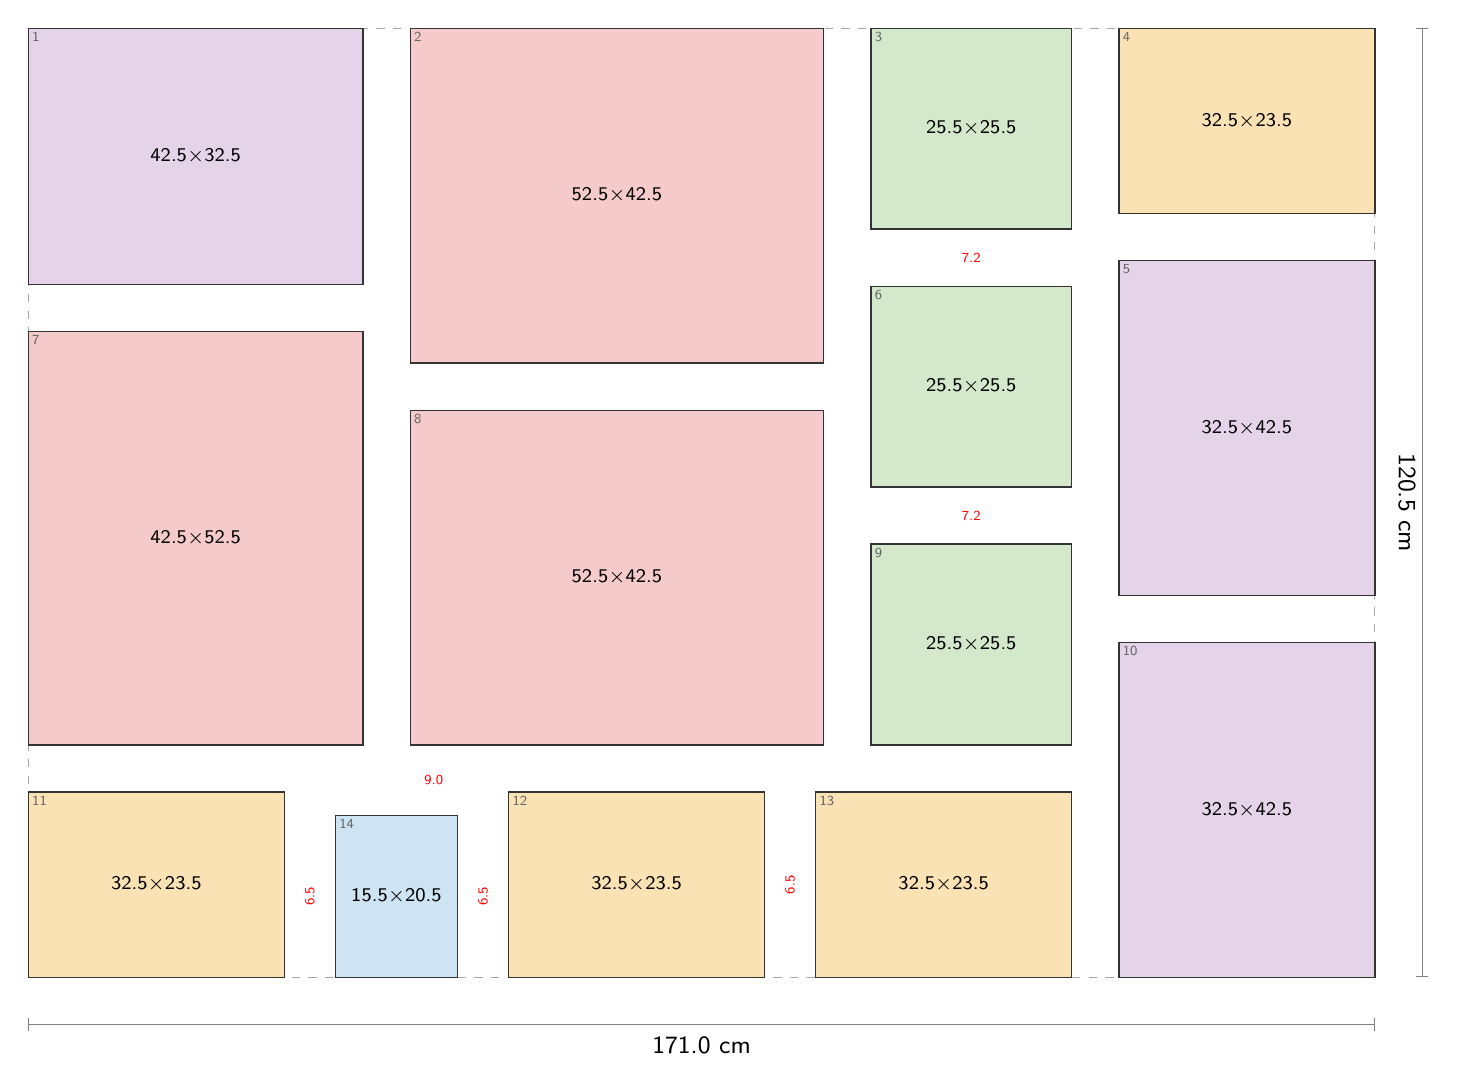
\begin{tikzpicture}[x=1mm, y=-1mm]
\draw[gray!70, dashed, line width=0.4pt] (0,0) rectangle (171.00,120.50);
\filldraw[fill=ft3, draw=black!80, line width=0.5pt] (0.00,0.00) rectangle (42.50,32.50);
\node[align=center, inner sep=0pt] at (21.25,16.25) {\scriptsize 42.5$\times$32.5};
\node[anchor=north west, inner sep=1.2pt, font=\tiny, text=black!60] at (0.00,0.00) {1};
\filldraw[fill=ft4, draw=black!80, line width=0.5pt] (48.50,0.00) rectangle (101.00,42.50);
\node[align=center, inner sep=0pt] at (74.75,21.25) {\scriptsize 52.5$\times$42.5};
\node[anchor=north west, inner sep=1.2pt, font=\tiny, text=black!60] at (48.50,0.00) {2};
\filldraw[fill=ft2, draw=black!80, line width=0.5pt] (107.00,0.00) rectangle (132.50,25.50);
\node[align=center, inner sep=0pt] at (119.75,12.75) {\scriptsize 25.5$\times$25.5};
\node[anchor=north west, inner sep=1.2pt, font=\tiny, text=black!60] at (107.00,0.00) {3};
\filldraw[fill=ft1, draw=black!80, line width=0.5pt] (138.50,0.00) rectangle (171.00,23.50);
\node[align=center, inner sep=0pt] at (154.75,11.75) {\scriptsize 32.5$\times$23.5};
\node[anchor=north west, inner sep=1.2pt, font=\tiny, text=black!60] at (138.50,0.00) {4};
\filldraw[fill=ft3, draw=black!80, line width=0.5pt] (138.50,29.50) rectangle (171.00,72.00);
\node[align=center, inner sep=0pt] at (154.75,50.75) {\scriptsize 32.5$\times$42.5};
\node[anchor=north west, inner sep=1.2pt, font=\tiny, text=black!60] at (138.50,29.50) {5};
\filldraw[fill=ft2, draw=black!80, line width=0.5pt] (107.00,32.75) rectangle (132.50,58.25);
\node[align=center, inner sep=0pt] at (119.75,45.50) {\scriptsize 25.5$\times$25.5};
\node[anchor=north west, inner sep=1.2pt, font=\tiny, text=black!60] at (107.00,32.75) {6};
\filldraw[fill=ft4, draw=black!80, line width=0.5pt] (0.00,38.50) rectangle (42.50,91.00);
\node[align=center, inner sep=0pt] at (21.25,64.75) {\scriptsize 42.5$\times$52.5};
\node[anchor=north west, inner sep=1.2pt, font=\tiny, text=black!60] at (0.00,38.50) {7};
\filldraw[fill=ft4, draw=black!80, line width=0.5pt] (48.50,48.50) rectangle (101.00,91.00);
\node[align=center, inner sep=0pt] at (74.75,69.75) {\scriptsize 52.5$\times$42.5};
\node[anchor=north west, inner sep=1.2pt, font=\tiny, text=black!60] at (48.50,48.50) {8};
\filldraw[fill=ft2, draw=black!80, line width=0.5pt] (107.00,65.50) rectangle (132.50,91.00);
\node[align=center, inner sep=0pt] at (119.75,78.25) {\scriptsize 25.5$\times$25.5};
\node[anchor=north west, inner sep=1.2pt, font=\tiny, text=black!60] at (107.00,65.50) {9};
\filldraw[fill=ft3, draw=black!80, line width=0.5pt] (138.50,78.00) rectangle (171.00,120.50);
\node[align=center, inner sep=0pt] at (154.75,99.25) {\scriptsize 32.5$\times$42.5};
\node[anchor=north west, inner sep=1.2pt, font=\tiny, text=black!60] at (138.50,78.00) {10};
\filldraw[fill=ft1, draw=black!80, line width=0.5pt] (0.00,97.00) rectangle (32.50,120.50);
\node[align=center, inner sep=0pt] at (16.25,108.75) {\scriptsize 32.5$\times$23.5};
\node[anchor=north west, inner sep=1.2pt, font=\tiny, text=black!60] at (0.00,97.00) {11};
\filldraw[fill=ft1, draw=black!80, line width=0.5pt] (61.00,97.00) rectangle (93.50,120.50);
\node[align=center, inner sep=0pt] at (77.25,108.75) {\scriptsize 32.5$\times$23.5};
\node[anchor=north west, inner sep=1.2pt, font=\tiny, text=black!60] at (61.00,97.00) {12};
\filldraw[fill=ft1, draw=black!80, line width=0.5pt] (100.00,97.00) rectangle (132.50,120.50);
\node[align=center, inner sep=0pt] at (116.25,108.75) {\scriptsize 32.5$\times$23.5};
\node[anchor=north west, inner sep=1.2pt, font=\tiny, text=black!60] at (100.00,97.00) {13};
\filldraw[fill=ft0, draw=black!80, line width=0.5pt] (39.00,100.00) rectangle (54.50,120.50);
\node[align=center, inner sep=0pt] at (46.75,110.25) {\scriptsize 15.5$\times$20.5};
\node[anchor=north west, inner sep=1.2pt, font=\tiny, text=black!60] at (39.00,100.00) {14};
\node[font=\tiny, text=red, fill=white, inner sep=0.3pt] at (119.75,29.12) {7.2};
\node[font=\tiny, text=red, fill=white, inner sep=0.3pt] at (119.75,61.88) {7.2};
\node[font=\tiny, text=red, fill=white, inner sep=0.3pt] at (51.50,95.50) {9.0};
\node[font=\tiny, text=red, fill=white, inner sep=0.3pt, rotate=90] at (35.75,110.25) {6.5};
\node[font=\tiny, text=red, fill=white, inner sep=0.3pt, rotate=90] at (96.75,108.75) {6.5};
\node[font=\tiny, text=red, fill=white, inner sep=0.3pt, rotate=90] at (57.75,110.25) {6.5};
\draw[Bar-Bar, gray] (0,126.50) -- (171.00,126.50) node[midway, below=1pt, font=\small, text=black] {171.0 cm};
\draw[Bar-Bar, gray] (177.00,0) -- (177.00,120.50) node[midway, right=1pt, font=\small, text=black, rotate=-90, anchor=north] {120.5 cm};
\end{tikzpicture}\\[4pt]
{\scriptsize Scale 1:10 (1 mm = 1 cm). Red numbers mark gaps that deviate from the nominal gap by more than 0.25 cm. Small grey numbers index the coordinate table.}
\end{minipage}\hfill
\begin{minipage}[t]{0.25\textwidth}\vspace{0pt}
\small
\begin{tabular}{@{}l l@{}}
\toprule
Outer size & 171.0 $\times$ 120.5 cm \\
Nominal gap & 6 cm \\
Actual gaps & 6.0 -- 9.0 cm \\
Max.\ deviation & 3.0 cm \\
Mean deviation & 0.29 cm \\
Border notches & none \\
Corners filled & 4 / 4 \\
Frames used & 14 of 28 \\
Large frames & {\scriptsize 3, touching 2$\times$ (95 cm), min.\ dist.\ 48 cm} \\
Entropy & 0.81 \\
\quad {\scriptsize mix / variety} & {\scriptsize 0.82 / 0.86} \\
\quad {\scriptsize stagger / lines} & {\scriptsize 0.55 / 1.00 (1 through)} \\
\bottomrule
\end{tabular}

\vspace{8pt}
\scriptsize
\begin{tabular}{@{}c l l r r@{}}
\toprule
 & outer w $\times$ h (cm) &  & used & have \\
\midrule
\tikz[baseline=-0.6ex]\fill[ft0,draw=black!60] (0,0) rectangle (1.2ex,1.2ex); & 20.5$\times$15.5 & L & 0 & 9 \\
\tikz[baseline=-0.6ex]\fill[ft0,draw=black!60] (0,0) rectangle (1.2ex,1.2ex); & 15.5$\times$20.5 & P & 1 & 2 \\
\tikz[baseline=-0.6ex]\fill[ft3,draw=black!60] (0,0) rectangle (1.2ex,1.2ex); & 32.5$\times$42.5 & P & 2 & 2 \\
\tikz[baseline=-0.6ex]\fill[ft3,draw=black!60] (0,0) rectangle (1.2ex,1.2ex); & 42.5$\times$32.5 & L & 1 & 1 \\
\tikz[baseline=-0.6ex]\fill[ft1,draw=black!60] (0,0) rectangle (1.2ex,1.2ex); & 32.5$\times$23.5 & L & 4 & 5 \\
\tikz[baseline=-0.6ex]\fill[ft1,draw=black!60] (0,0) rectangle (1.2ex,1.2ex); & 23.5$\times$32.5 & P & 0 & 1 \\
\tikz[baseline=-0.6ex]\fill[ft2,draw=black!60] (0,0) rectangle (1.2ex,1.2ex); & 25.5$\times$25.5 &  & 3 & 5 \\
\tikz[baseline=-0.6ex]\fill[ft4,draw=black!60] (0,0) rectangle (1.2ex,1.2ex); & 42.5$\times$52.5 & P & 1 & 1 \\
\tikz[baseline=-0.6ex]\fill[ft4,draw=black!60] (0,0) rectangle (1.2ex,1.2ex); & 52.5$\times$42.5 & L & 2 & 2 \\
\bottomrule
\end{tabular}

\vspace{8pt}
{\bfseries Positions} (top-left corner, cm)\\[2pt]
\tiny
\begin{tabular}{@{}r l r r@{}}
\toprule
\# & frame w $\times$ h & x & y \\
\midrule
1 & 42.5 $\times$ 32.5 & 0.0 & 0.0 \\
2 & 52.5 $\times$ 42.5 & 48.5 & 0.0 \\
3 & 25.5 $\times$ 25.5 & 107.0 & 0.0 \\
4 & 32.5 $\times$ 23.5 & 138.5 & 0.0 \\
5 & 32.5 $\times$ 42.5 & 138.5 & 29.5 \\
6 & 25.5 $\times$ 25.5 & 107.0 & 32.8 \\
7 & 42.5 $\times$ 52.5 & 0.0 & 38.5 \\
8 & 52.5 $\times$ 42.5 & 48.5 & 48.5 \\
9 & 25.5 $\times$ 25.5 & 107.0 & 65.5 \\
10 & 32.5 $\times$ 42.5 & 138.5 & 78.0 \\
11 & 32.5 $\times$ 23.5 & 0.0 & 97.0 \\
12 & 32.5 $\times$ 23.5 & 61.0 & 97.0 \\
13 & 32.5 $\times$ 23.5 & 100.0 & 97.0 \\
14 & 15.5 $\times$ 20.5 & 39.0 & 100.0 \\
\bottomrule
\end{tabular}
\end{minipage}
\clearpage

\phantomsection\addcontentsline{toc}{subsection}{Layout 15: 187.5 \texorpdfstring{$\times$}{x} 130.0 cm, 26 frames, gap 2 cm, max.\ deviation 3.5 cm}
\label{lay:free-gap:15}
\begin{minipage}[t]{0.74\textwidth}\vspace{0pt}
{\LARGE\bfseries Layout 15}\hspace{1.5em}{\large 187.5 $\times$ 130.0 cm \quad gap 2 cm \quad 26 frames}\\[8pt]
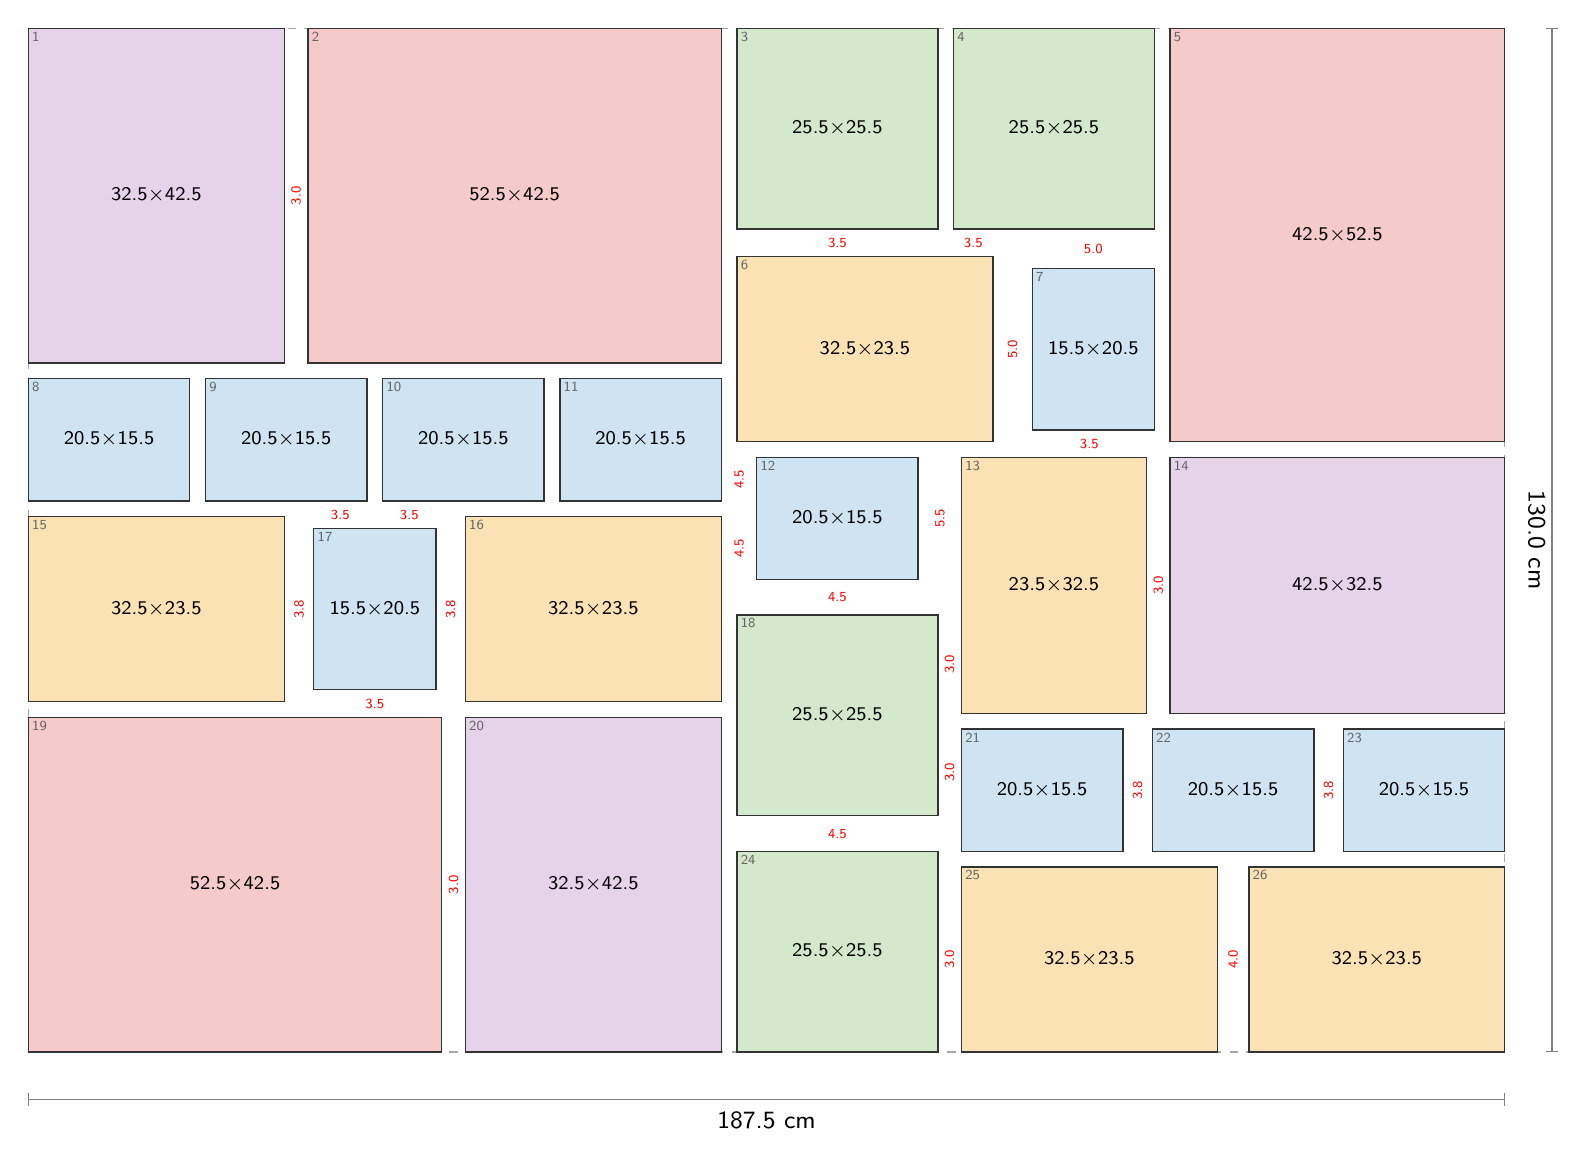
\begin{tikzpicture}[x=1mm, y=-1mm]
\draw[gray!70, dashed, line width=0.4pt] (0,0) rectangle (187.50,130.00);
\filldraw[fill=ft3, draw=black!80, line width=0.5pt] (0.00,0.00) rectangle (32.50,42.50);
\node[align=center, inner sep=0pt] at (16.25,21.25) {\scriptsize 32.5$\times$42.5};
\node[anchor=north west, inner sep=1.2pt, font=\tiny, text=black!60] at (0.00,0.00) {1};
\filldraw[fill=ft4, draw=black!80, line width=0.5pt] (35.50,0.00) rectangle (88.00,42.50);
\node[align=center, inner sep=0pt] at (61.75,21.25) {\scriptsize 52.5$\times$42.5};
\node[anchor=north west, inner sep=1.2pt, font=\tiny, text=black!60] at (35.50,0.00) {2};
\filldraw[fill=ft2, draw=black!80, line width=0.5pt] (90.00,0.00) rectangle (115.50,25.50);
\node[align=center, inner sep=0pt] at (102.75,12.75) {\scriptsize 25.5$\times$25.5};
\node[anchor=north west, inner sep=1.2pt, font=\tiny, text=black!60] at (90.00,0.00) {3};
\filldraw[fill=ft2, draw=black!80, line width=0.5pt] (117.50,0.00) rectangle (143.00,25.50);
\node[align=center, inner sep=0pt] at (130.25,12.75) {\scriptsize 25.5$\times$25.5};
\node[anchor=north west, inner sep=1.2pt, font=\tiny, text=black!60] at (117.50,0.00) {4};
\filldraw[fill=ft4, draw=black!80, line width=0.5pt] (145.00,0.00) rectangle (187.50,52.50);
\node[align=center, inner sep=0pt] at (166.25,26.25) {\scriptsize 42.5$\times$52.5};
\node[anchor=north west, inner sep=1.2pt, font=\tiny, text=black!60] at (145.00,0.00) {5};
\filldraw[fill=ft1, draw=black!80, line width=0.5pt] (90.00,29.00) rectangle (122.50,52.50);
\node[align=center, inner sep=0pt] at (106.25,40.75) {\scriptsize 32.5$\times$23.5};
\node[anchor=north west, inner sep=1.2pt, font=\tiny, text=black!60] at (90.00,29.00) {6};
\filldraw[fill=ft0, draw=black!80, line width=0.5pt] (127.50,30.50) rectangle (143.00,51.00);
\node[align=center, inner sep=0pt] at (135.25,40.75) {\scriptsize 15.5$\times$20.5};
\node[anchor=north west, inner sep=1.2pt, font=\tiny, text=black!60] at (127.50,30.50) {7};
\filldraw[fill=ft0, draw=black!80, line width=0.5pt] (0.00,44.50) rectangle (20.50,60.00);
\node[align=center, inner sep=0pt] at (10.25,52.25) {\scriptsize 20.5$\times$15.5};
\node[anchor=north west, inner sep=1.2pt, font=\tiny, text=black!60] at (0.00,44.50) {8};
\filldraw[fill=ft0, draw=black!80, line width=0.5pt] (22.50,44.50) rectangle (43.00,60.00);
\node[align=center, inner sep=0pt] at (32.75,52.25) {\scriptsize 20.5$\times$15.5};
\node[anchor=north west, inner sep=1.2pt, font=\tiny, text=black!60] at (22.50,44.50) {9};
\filldraw[fill=ft0, draw=black!80, line width=0.5pt] (45.00,44.50) rectangle (65.50,60.00);
\node[align=center, inner sep=0pt] at (55.25,52.25) {\scriptsize 20.5$\times$15.5};
\node[anchor=north west, inner sep=1.2pt, font=\tiny, text=black!60] at (45.00,44.50) {10};
\filldraw[fill=ft0, draw=black!80, line width=0.5pt] (67.50,44.50) rectangle (88.00,60.00);
\node[align=center, inner sep=0pt] at (77.75,52.25) {\scriptsize 20.5$\times$15.5};
\node[anchor=north west, inner sep=1.2pt, font=\tiny, text=black!60] at (67.50,44.50) {11};
\filldraw[fill=ft0, draw=black!80, line width=0.5pt] (92.50,54.50) rectangle (113.00,70.00);
\node[align=center, inner sep=0pt] at (102.75,62.25) {\scriptsize 20.5$\times$15.5};
\node[anchor=north west, inner sep=1.2pt, font=\tiny, text=black!60] at (92.50,54.50) {12};
\filldraw[fill=ft1, draw=black!80, line width=0.5pt] (118.50,54.50) rectangle (142.00,87.00);
\node[align=center, inner sep=0pt] at (130.25,70.75) {\scriptsize 23.5$\times$32.5};
\node[anchor=north west, inner sep=1.2pt, font=\tiny, text=black!60] at (118.50,54.50) {13};
\filldraw[fill=ft3, draw=black!80, line width=0.5pt] (145.00,54.50) rectangle (187.50,87.00);
\node[align=center, inner sep=0pt] at (166.25,70.75) {\scriptsize 42.5$\times$32.5};
\node[anchor=north west, inner sep=1.2pt, font=\tiny, text=black!60] at (145.00,54.50) {14};
\filldraw[fill=ft1, draw=black!80, line width=0.5pt] (0.00,62.00) rectangle (32.50,85.50);
\node[align=center, inner sep=0pt] at (16.25,73.75) {\scriptsize 32.5$\times$23.5};
\node[anchor=north west, inner sep=1.2pt, font=\tiny, text=black!60] at (0.00,62.00) {15};
\filldraw[fill=ft1, draw=black!80, line width=0.5pt] (55.50,62.00) rectangle (88.00,85.50);
\node[align=center, inner sep=0pt] at (71.75,73.75) {\scriptsize 32.5$\times$23.5};
\node[anchor=north west, inner sep=1.2pt, font=\tiny, text=black!60] at (55.50,62.00) {16};
\filldraw[fill=ft0, draw=black!80, line width=0.5pt] (36.25,63.50) rectangle (51.75,84.00);
\node[align=center, inner sep=0pt] at (44.00,73.75) {\scriptsize 15.5$\times$20.5};
\node[anchor=north west, inner sep=1.2pt, font=\tiny, text=black!60] at (36.25,63.50) {17};
\filldraw[fill=ft2, draw=black!80, line width=0.5pt] (90.00,74.50) rectangle (115.50,100.00);
\node[align=center, inner sep=0pt] at (102.75,87.25) {\scriptsize 25.5$\times$25.5};
\node[anchor=north west, inner sep=1.2pt, font=\tiny, text=black!60] at (90.00,74.50) {18};
\filldraw[fill=ft4, draw=black!80, line width=0.5pt] (0.00,87.50) rectangle (52.50,130.00);
\node[align=center, inner sep=0pt] at (26.25,108.75) {\scriptsize 52.5$\times$42.5};
\node[anchor=north west, inner sep=1.2pt, font=\tiny, text=black!60] at (0.00,87.50) {19};
\filldraw[fill=ft3, draw=black!80, line width=0.5pt] (55.50,87.50) rectangle (88.00,130.00);
\node[align=center, inner sep=0pt] at (71.75,108.75) {\scriptsize 32.5$\times$42.5};
\node[anchor=north west, inner sep=1.2pt, font=\tiny, text=black!60] at (55.50,87.50) {20};
\filldraw[fill=ft0, draw=black!80, line width=0.5pt] (118.50,89.00) rectangle (139.00,104.50);
\node[align=center, inner sep=0pt] at (128.75,96.75) {\scriptsize 20.5$\times$15.5};
\node[anchor=north west, inner sep=1.2pt, font=\tiny, text=black!60] at (118.50,89.00) {21};
\filldraw[fill=ft0, draw=black!80, line width=0.5pt] (142.75,89.00) rectangle (163.25,104.50);
\node[align=center, inner sep=0pt] at (153.00,96.75) {\scriptsize 20.5$\times$15.5};
\node[anchor=north west, inner sep=1.2pt, font=\tiny, text=black!60] at (142.75,89.00) {22};
\filldraw[fill=ft0, draw=black!80, line width=0.5pt] (167.00,89.00) rectangle (187.50,104.50);
\node[align=center, inner sep=0pt] at (177.25,96.75) {\scriptsize 20.5$\times$15.5};
\node[anchor=north west, inner sep=1.2pt, font=\tiny, text=black!60] at (167.00,89.00) {23};
\filldraw[fill=ft2, draw=black!80, line width=0.5pt] (90.00,104.50) rectangle (115.50,130.00);
\node[align=center, inner sep=0pt] at (102.75,117.25) {\scriptsize 25.5$\times$25.5};
\node[anchor=north west, inner sep=1.2pt, font=\tiny, text=black!60] at (90.00,104.50) {24};
\filldraw[fill=ft1, draw=black!80, line width=0.5pt] (118.50,106.50) rectangle (151.00,130.00);
\node[align=center, inner sep=0pt] at (134.75,118.25) {\scriptsize 32.5$\times$23.5};
\node[anchor=north west, inner sep=1.2pt, font=\tiny, text=black!60] at (118.50,106.50) {25};
\filldraw[fill=ft1, draw=black!80, line width=0.5pt] (155.00,106.50) rectangle (187.50,130.00);
\node[align=center, inner sep=0pt] at (171.25,118.25) {\scriptsize 32.5$\times$23.5};
\node[anchor=north west, inner sep=1.2pt, font=\tiny, text=black!60] at (155.00,106.50) {26};
\node[font=\tiny, text=red, fill=white, inner sep=0.3pt, rotate=90] at (34.00,21.25) {3.0};
\node[font=\tiny, text=red, fill=white, inner sep=0.3pt] at (102.75,27.25) {3.5};
\node[font=\tiny, text=red, fill=white, inner sep=0.3pt] at (120.00,27.25) {3.5};
\node[font=\tiny, text=red, fill=white, inner sep=0.3pt] at (135.25,28.00) {5.0};
\node[font=\tiny, text=red, fill=white, inner sep=0.3pt, rotate=90] at (125.00,40.75) {5.0};
\node[font=\tiny, text=red, fill=white, inner sep=0.3pt] at (134.75,52.75) {3.5};
\node[font=\tiny, text=red, fill=white, inner sep=0.3pt] at (39.62,61.75) {3.5};
\node[font=\tiny, text=red, fill=white, inner sep=0.3pt] at (48.38,61.75) {3.5};
\node[font=\tiny, text=red, fill=white, inner sep=0.3pt, rotate=90] at (90.25,57.25) {4.5};
\node[font=\tiny, text=red, fill=white, inner sep=0.3pt, rotate=90] at (115.75,62.25) {5.5};
\node[font=\tiny, text=red, fill=white, inner sep=0.3pt] at (102.75,72.25) {4.5};
\node[font=\tiny, text=red, fill=white, inner sep=0.3pt, rotate=90] at (143.50,70.75) {3.0};
\node[font=\tiny, text=red, fill=white, inner sep=0.3pt, rotate=90] at (34.38,73.75) {3.8};
\node[font=\tiny, text=red, fill=white, inner sep=0.3pt, rotate=90] at (90.25,66.00) {4.5};
\node[font=\tiny, text=red, fill=white, inner sep=0.3pt, rotate=90] at (53.62,73.75) {3.8};
\node[font=\tiny, text=red, fill=white, inner sep=0.3pt] at (44.00,85.75) {3.5};
\node[font=\tiny, text=red, fill=white, inner sep=0.3pt, rotate=90] at (117.00,80.75) {3.0};
\node[font=\tiny, text=red, fill=white, inner sep=0.3pt, rotate=90] at (117.00,94.50) {3.0};
\node[font=\tiny, text=red, fill=white, inner sep=0.3pt] at (102.75,102.25) {4.5};
\node[font=\tiny, text=red, fill=white, inner sep=0.3pt, rotate=90] at (54.00,108.75) {3.0};
\node[font=\tiny, text=red, fill=white, inner sep=0.3pt, rotate=90] at (140.88,96.75) {3.8};
\node[font=\tiny, text=red, fill=white, inner sep=0.3pt, rotate=90] at (165.12,96.75) {3.8};
\node[font=\tiny, text=red, fill=white, inner sep=0.3pt, rotate=90] at (117.00,118.25) {3.0};
\node[font=\tiny, text=red, fill=white, inner sep=0.3pt, rotate=90] at (153.00,118.25) {4.0};
\draw[Bar-Bar, gray] (0,136.00) -- (187.50,136.00) node[midway, below=1pt, font=\small, text=black] {187.5 cm};
\draw[Bar-Bar, gray] (193.50,0) -- (193.50,130.00) node[midway, right=1pt, font=\small, text=black, rotate=-90, anchor=north] {130.0 cm};
\end{tikzpicture}\\[4pt]
{\scriptsize Scale 1:10 (1 mm = 1 cm). Red numbers mark gaps that deviate from the nominal gap by more than 0.25 cm. Small grey numbers index the coordinate table.}
\end{minipage}\hfill
\begin{minipage}[t]{0.25\textwidth}\vspace{0pt}
\small
\begin{tabular}{@{}l l@{}}
\toprule
Outer size & 187.5 $\times$ 130.0 cm \\
Nominal gap & 2 cm \\
Actual gaps & 2.0 -- 5.5 cm \\
Max.\ deviation & 3.5 cm \\
Mean deviation & 0.78 cm \\
Border notches & bottom 4 cm \\
Corners filled & 4 / 4 \\
Frames used & 26 of 28 \\
Large frames & {\scriptsize 3, not touching, min.\ dist.\ 94 cm} \\
Entropy & 0.83 \\
\quad {\scriptsize mix / variety} & {\scriptsize 0.88 / 0.89} \\
\quad {\scriptsize stagger / lines} & {\scriptsize 0.53 / 1.00 (1 through)} \\
\bottomrule
\end{tabular}

\vspace{8pt}
\scriptsize
\begin{tabular}{@{}c l l r r@{}}
\toprule
 & outer w $\times$ h (cm) &  & used & have \\
\midrule
\tikz[baseline=-0.6ex]\fill[ft0,draw=black!60] (0,0) rectangle (1.2ex,1.2ex); & 20.5$\times$15.5 & L & 8 & 9 \\
\tikz[baseline=-0.6ex]\fill[ft0,draw=black!60] (0,0) rectangle (1.2ex,1.2ex); & 15.5$\times$20.5 & P & 2 & 2 \\
\tikz[baseline=-0.6ex]\fill[ft3,draw=black!60] (0,0) rectangle (1.2ex,1.2ex); & 32.5$\times$42.5 & P & 2 & 2 \\
\tikz[baseline=-0.6ex]\fill[ft3,draw=black!60] (0,0) rectangle (1.2ex,1.2ex); & 42.5$\times$32.5 & L & 1 & 1 \\
\tikz[baseline=-0.6ex]\fill[ft1,draw=black!60] (0,0) rectangle (1.2ex,1.2ex); & 32.5$\times$23.5 & L & 5 & 5 \\
\tikz[baseline=-0.6ex]\fill[ft1,draw=black!60] (0,0) rectangle (1.2ex,1.2ex); & 23.5$\times$32.5 & P & 1 & 1 \\
\tikz[baseline=-0.6ex]\fill[ft2,draw=black!60] (0,0) rectangle (1.2ex,1.2ex); & 25.5$\times$25.5 &  & 4 & 5 \\
\tikz[baseline=-0.6ex]\fill[ft4,draw=black!60] (0,0) rectangle (1.2ex,1.2ex); & 42.5$\times$52.5 & P & 1 & 1 \\
\tikz[baseline=-0.6ex]\fill[ft4,draw=black!60] (0,0) rectangle (1.2ex,1.2ex); & 52.5$\times$42.5 & L & 2 & 2 \\
\bottomrule
\end{tabular}

\vspace{8pt}
{\bfseries Positions} (top-left corner, cm)\\[2pt]
\tiny
\begin{tabular}{@{}r l r r@{}}
\toprule
\# & frame w $\times$ h & x & y \\
\midrule
1 & 32.5 $\times$ 42.5 & 0.0 & 0.0 \\
2 & 52.5 $\times$ 42.5 & 35.5 & 0.0 \\
3 & 25.5 $\times$ 25.5 & 90.0 & 0.0 \\
4 & 25.5 $\times$ 25.5 & 117.5 & 0.0 \\
5 & 42.5 $\times$ 52.5 & 145.0 & 0.0 \\
6 & 32.5 $\times$ 23.5 & 90.0 & 29.0 \\
7 & 15.5 $\times$ 20.5 & 127.5 & 30.5 \\
8 & 20.5 $\times$ 15.5 & 0.0 & 44.5 \\
9 & 20.5 $\times$ 15.5 & 22.5 & 44.5 \\
10 & 20.5 $\times$ 15.5 & 45.0 & 44.5 \\
11 & 20.5 $\times$ 15.5 & 67.5 & 44.5 \\
12 & 20.5 $\times$ 15.5 & 92.5 & 54.5 \\
13 & 23.5 $\times$ 32.5 & 118.5 & 54.5 \\
14 & 42.5 $\times$ 32.5 & 145.0 & 54.5 \\
15 & 32.5 $\times$ 23.5 & 0.0 & 62.0 \\
16 & 32.5 $\times$ 23.5 & 55.5 & 62.0 \\
17 & 15.5 $\times$ 20.5 & 36.2 & 63.5 \\
18 & 25.5 $\times$ 25.5 & 90.0 & 74.5 \\
19 & 52.5 $\times$ 42.5 & 0.0 & 87.5 \\
20 & 32.5 $\times$ 42.5 & 55.5 & 87.5 \\
21 & 20.5 $\times$ 15.5 & 118.5 & 89.0 \\
22 & 20.5 $\times$ 15.5 & 142.8 & 89.0 \\
23 & 20.5 $\times$ 15.5 & 167.0 & 89.0 \\
24 & 25.5 $\times$ 25.5 & 90.0 & 104.5 \\
25 & 32.5 $\times$ 23.5 & 118.5 & 106.5 \\
26 & 32.5 $\times$ 23.5 & 155.0 & 106.5 \\
\bottomrule
\end{tabular}
\end{minipage}
\clearpage

\phantomsection\addcontentsline{toc}{subsection}{Layout 16: 180.0 \texorpdfstring{$\times$}{x} 114.5 cm, 25 frames, gap 2 cm, max.\ deviation 3.0 cm}
\label{lay:free-gap:16}
\begin{minipage}[t]{0.74\textwidth}\vspace{0pt}
{\LARGE\bfseries Layout 16}\hspace{1.5em}{\large 180.0 $\times$ 114.5 cm \quad gap 2 cm \quad 25 frames}\\[8pt]
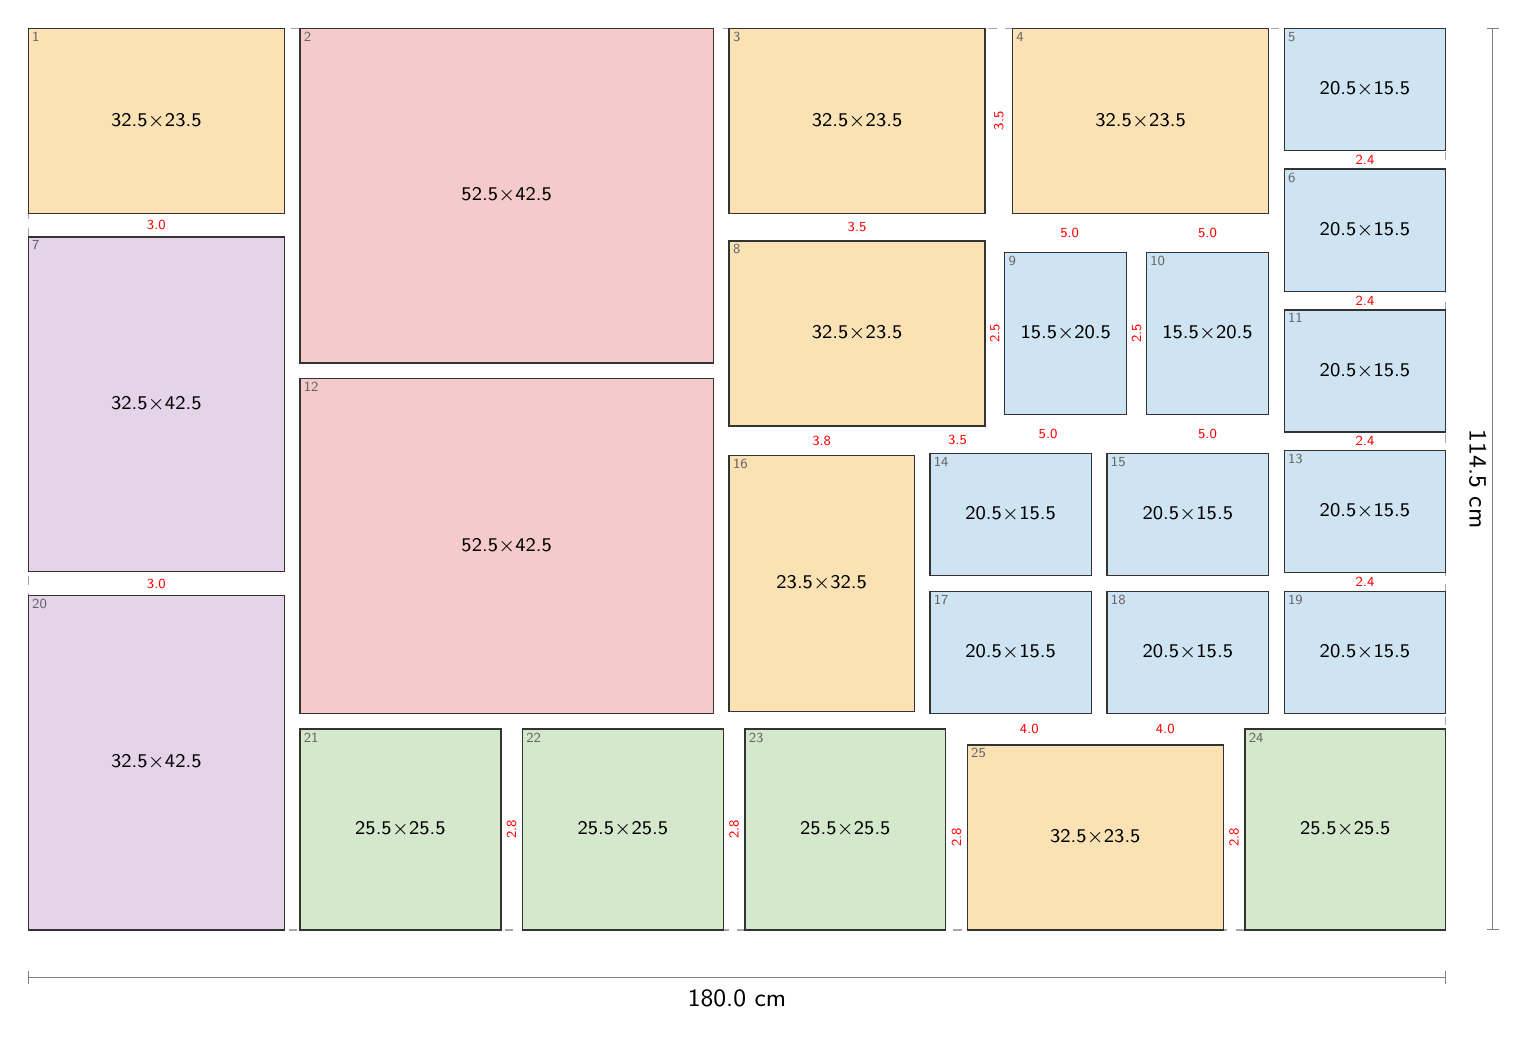
\begin{tikzpicture}[x=1mm, y=-1mm]
\draw[gray!70, dashed, line width=0.4pt] (0,0) rectangle (180.00,114.50);
\filldraw[fill=ft1, draw=black!80, line width=0.5pt] (0.00,0.00) rectangle (32.50,23.50);
\node[align=center, inner sep=0pt] at (16.25,11.75) {\scriptsize 32.5$\times$23.5};
\node[anchor=north west, inner sep=1.2pt, font=\tiny, text=black!60] at (0.00,0.00) {1};
\filldraw[fill=ft4, draw=black!80, line width=0.5pt] (34.50,0.00) rectangle (87.00,42.50);
\node[align=center, inner sep=0pt] at (60.75,21.25) {\scriptsize 52.5$\times$42.5};
\node[anchor=north west, inner sep=1.2pt, font=\tiny, text=black!60] at (34.50,0.00) {2};
\filldraw[fill=ft1, draw=black!80, line width=0.5pt] (89.00,0.00) rectangle (121.50,23.50);
\node[align=center, inner sep=0pt] at (105.25,11.75) {\scriptsize 32.5$\times$23.5};
\node[anchor=north west, inner sep=1.2pt, font=\tiny, text=black!60] at (89.00,0.00) {3};
\filldraw[fill=ft1, draw=black!80, line width=0.5pt] (125.00,0.00) rectangle (157.50,23.50);
\node[align=center, inner sep=0pt] at (141.25,11.75) {\scriptsize 32.5$\times$23.5};
\node[anchor=north west, inner sep=1.2pt, font=\tiny, text=black!60] at (125.00,0.00) {4};
\filldraw[fill=ft0, draw=black!80, line width=0.5pt] (159.50,0.00) rectangle (180.00,15.50);
\node[align=center, inner sep=0pt] at (169.75,7.75) {\scriptsize 20.5$\times$15.5};
\node[anchor=north west, inner sep=1.2pt, font=\tiny, text=black!60] at (159.50,0.00) {5};
\filldraw[fill=ft0, draw=black!80, line width=0.5pt] (159.50,17.88) rectangle (180.00,33.38);
\node[align=center, inner sep=0pt] at (169.75,25.62) {\scriptsize 20.5$\times$15.5};
\node[anchor=north west, inner sep=1.2pt, font=\tiny, text=black!60] at (159.50,17.88) {6};
\filldraw[fill=ft3, draw=black!80, line width=0.5pt] (0.00,26.50) rectangle (32.50,69.00);
\node[align=center, inner sep=0pt] at (16.25,47.75) {\scriptsize 32.5$\times$42.5};
\node[anchor=north west, inner sep=1.2pt, font=\tiny, text=black!60] at (0.00,26.50) {7};
\filldraw[fill=ft1, draw=black!80, line width=0.5pt] (89.00,27.00) rectangle (121.50,50.50);
\node[align=center, inner sep=0pt] at (105.25,38.75) {\scriptsize 32.5$\times$23.5};
\node[anchor=north west, inner sep=1.2pt, font=\tiny, text=black!60] at (89.00,27.00) {8};
\filldraw[fill=ft0, draw=black!80, line width=0.5pt] (124.00,28.50) rectangle (139.50,49.00);
\node[align=center, inner sep=0pt] at (131.75,38.75) {\scriptsize 15.5$\times$20.5};
\node[anchor=north west, inner sep=1.2pt, font=\tiny, text=black!60] at (124.00,28.50) {9};
\filldraw[fill=ft0, draw=black!80, line width=0.5pt] (142.00,28.50) rectangle (157.50,49.00);
\node[align=center, inner sep=0pt] at (149.75,38.75) {\scriptsize 15.5$\times$20.5};
\node[anchor=north west, inner sep=1.2pt, font=\tiny, text=black!60] at (142.00,28.50) {10};
\filldraw[fill=ft0, draw=black!80, line width=0.5pt] (159.50,35.75) rectangle (180.00,51.25);
\node[align=center, inner sep=0pt] at (169.75,43.50) {\scriptsize 20.5$\times$15.5};
\node[anchor=north west, inner sep=1.2pt, font=\tiny, text=black!60] at (159.50,35.75) {11};
\filldraw[fill=ft4, draw=black!80, line width=0.5pt] (34.50,44.50) rectangle (87.00,87.00);
\node[align=center, inner sep=0pt] at (60.75,65.75) {\scriptsize 52.5$\times$42.5};
\node[anchor=north west, inner sep=1.2pt, font=\tiny, text=black!60] at (34.50,44.50) {12};
\filldraw[fill=ft0, draw=black!80, line width=0.5pt] (159.50,53.62) rectangle (180.00,69.12);
\node[align=center, inner sep=0pt] at (169.75,61.38) {\scriptsize 20.5$\times$15.5};
\node[anchor=north west, inner sep=1.2pt, font=\tiny, text=black!60] at (159.50,53.62) {13};
\filldraw[fill=ft0, draw=black!80, line width=0.5pt] (114.50,54.00) rectangle (135.00,69.50);
\node[align=center, inner sep=0pt] at (124.75,61.75) {\scriptsize 20.5$\times$15.5};
\node[anchor=north west, inner sep=1.2pt, font=\tiny, text=black!60] at (114.50,54.00) {14};
\filldraw[fill=ft0, draw=black!80, line width=0.5pt] (137.00,54.00) rectangle (157.50,69.50);
\node[align=center, inner sep=0pt] at (147.25,61.75) {\scriptsize 20.5$\times$15.5};
\node[anchor=north west, inner sep=1.2pt, font=\tiny, text=black!60] at (137.00,54.00) {15};
\filldraw[fill=ft1, draw=black!80, line width=0.5pt] (89.00,54.25) rectangle (112.50,86.75);
\node[align=center, inner sep=0pt] at (100.75,70.50) {\scriptsize 23.5$\times$32.5};
\node[anchor=north west, inner sep=1.2pt, font=\tiny, text=black!60] at (89.00,54.25) {16};
\filldraw[fill=ft0, draw=black!80, line width=0.5pt] (114.50,71.50) rectangle (135.00,87.00);
\node[align=center, inner sep=0pt] at (124.75,79.25) {\scriptsize 20.5$\times$15.5};
\node[anchor=north west, inner sep=1.2pt, font=\tiny, text=black!60] at (114.50,71.50) {17};
\filldraw[fill=ft0, draw=black!80, line width=0.5pt] (137.00,71.50) rectangle (157.50,87.00);
\node[align=center, inner sep=0pt] at (147.25,79.25) {\scriptsize 20.5$\times$15.5};
\node[anchor=north west, inner sep=1.2pt, font=\tiny, text=black!60] at (137.00,71.50) {18};
\filldraw[fill=ft0, draw=black!80, line width=0.5pt] (159.50,71.50) rectangle (180.00,87.00);
\node[align=center, inner sep=0pt] at (169.75,79.25) {\scriptsize 20.5$\times$15.5};
\node[anchor=north west, inner sep=1.2pt, font=\tiny, text=black!60] at (159.50,71.50) {19};
\filldraw[fill=ft3, draw=black!80, line width=0.5pt] (0.00,72.00) rectangle (32.50,114.50);
\node[align=center, inner sep=0pt] at (16.25,93.25) {\scriptsize 32.5$\times$42.5};
\node[anchor=north west, inner sep=1.2pt, font=\tiny, text=black!60] at (0.00,72.00) {20};
\filldraw[fill=ft2, draw=black!80, line width=0.5pt] (34.50,89.00) rectangle (60.00,114.50);
\node[align=center, inner sep=0pt] at (47.25,101.75) {\scriptsize 25.5$\times$25.5};
\node[anchor=north west, inner sep=1.2pt, font=\tiny, text=black!60] at (34.50,89.00) {21};
\filldraw[fill=ft2, draw=black!80, line width=0.5pt] (62.75,89.00) rectangle (88.25,114.50);
\node[align=center, inner sep=0pt] at (75.50,101.75) {\scriptsize 25.5$\times$25.5};
\node[anchor=north west, inner sep=1.2pt, font=\tiny, text=black!60] at (62.75,89.00) {22};
\filldraw[fill=ft2, draw=black!80, line width=0.5pt] (91.00,89.00) rectangle (116.50,114.50);
\node[align=center, inner sep=0pt] at (103.75,101.75) {\scriptsize 25.5$\times$25.5};
\node[anchor=north west, inner sep=1.2pt, font=\tiny, text=black!60] at (91.00,89.00) {23};
\filldraw[fill=ft2, draw=black!80, line width=0.5pt] (154.50,89.00) rectangle (180.00,114.50);
\node[align=center, inner sep=0pt] at (167.25,101.75) {\scriptsize 25.5$\times$25.5};
\node[anchor=north west, inner sep=1.2pt, font=\tiny, text=black!60] at (154.50,89.00) {24};
\filldraw[fill=ft1, draw=black!80, line width=0.5pt] (119.25,91.00) rectangle (151.75,114.50);
\node[align=center, inner sep=0pt] at (135.50,102.75) {\scriptsize 32.5$\times$23.5};
\node[anchor=north west, inner sep=1.2pt, font=\tiny, text=black!60] at (119.25,91.00) {25};
\node[font=\tiny, text=red, fill=white, inner sep=0.3pt] at (16.25,25.00) {3.0};
\node[font=\tiny, text=red, fill=white, inner sep=0.3pt, rotate=90] at (123.25,11.75) {3.5};
\node[font=\tiny, text=red, fill=white, inner sep=0.3pt] at (105.25,25.25) {3.5};
\node[font=\tiny, text=red, fill=white, inner sep=0.3pt] at (132.25,26.00) {5.0};
\node[font=\tiny, text=red, fill=white, inner sep=0.3pt] at (149.75,26.00) {5.0};
\node[font=\tiny, text=red, fill=white, inner sep=0.3pt] at (169.75,16.69) {2.4};
\node[font=\tiny, text=red, fill=white, inner sep=0.3pt] at (169.75,34.56) {2.4};
\node[font=\tiny, text=red, fill=white, inner sep=0.3pt] at (16.25,70.50) {3.0};
\node[font=\tiny, text=red, fill=white, inner sep=0.3pt, rotate=90] at (122.75,38.75) {2.5};
\node[font=\tiny, text=red, fill=white, inner sep=0.3pt] at (118.00,52.25) {3.5};
\node[font=\tiny, text=red, fill=white, inner sep=0.3pt] at (100.75,52.38) {3.8};
\node[font=\tiny, text=red, fill=white, inner sep=0.3pt, rotate=90] at (140.75,38.75) {2.5};
\node[font=\tiny, text=red, fill=white, inner sep=0.3pt] at (129.50,51.50) {5.0};
\node[font=\tiny, text=red, fill=white, inner sep=0.3pt] at (149.75,51.50) {5.0};
\node[font=\tiny, text=red, fill=white, inner sep=0.3pt] at (169.75,52.44) {2.4};
\node[font=\tiny, text=red, fill=white, inner sep=0.3pt] at (169.75,70.31) {2.4};
\node[font=\tiny, text=red, fill=white, inner sep=0.3pt] at (127.12,89.00) {4.0};
\node[font=\tiny, text=red, fill=white, inner sep=0.3pt] at (144.38,89.00) {4.0};
\node[font=\tiny, text=red, fill=white, inner sep=0.3pt, rotate=90] at (61.38,101.75) {2.8};
\node[font=\tiny, text=red, fill=white, inner sep=0.3pt, rotate=90] at (89.62,101.75) {2.8};
\node[font=\tiny, text=red, fill=white, inner sep=0.3pt, rotate=90] at (117.88,102.75) {2.8};
\node[font=\tiny, text=red, fill=white, inner sep=0.3pt, rotate=90] at (153.12,102.75) {2.8};
\draw[Bar-Bar, gray] (0,120.50) -- (180.00,120.50) node[midway, below=1pt, font=\small, text=black] {180.0 cm};
\draw[Bar-Bar, gray] (186.00,0) -- (186.00,114.50) node[midway, right=1pt, font=\small, text=black, rotate=-90, anchor=north] {114.5 cm};
\end{tikzpicture}\\[4pt]
{\scriptsize Scale 1:10 (1 mm = 1 cm). Red numbers mark gaps that deviate from the nominal gap by more than 0.25 cm. Small grey numbers index the coordinate table.}
\end{minipage}\hfill
\begin{minipage}[t]{0.25\textwidth}\vspace{0pt}
\small
\begin{tabular}{@{}l l@{}}
\toprule
Outer size & 180.0 $\times$ 114.5 cm \\
Nominal gap & 2 cm \\
Actual gaps & 2.0 -- 5.0 cm \\
Max.\ deviation & 3.0 cm \\
Mean deviation & 0.64 cm \\
Border notches & top 4 cm \\
Corners filled & 4 / 4 \\
Frames used & 25 of 28 \\
Large frames & {\scriptsize 2, touching 1$\times$ (52 cm), min.\ dist.\ 44 cm} \\
Entropy & 0.66 \\
\quad {\scriptsize mix / variety} & {\scriptsize 0.78 / 0.59} \\
\quad {\scriptsize stagger / lines} & {\scriptsize 0.52 / 0.75 (2 through)} \\
\bottomrule
\end{tabular}

\vspace{8pt}
\scriptsize
\begin{tabular}{@{}c l l r r@{}}
\toprule
 & outer w $\times$ h (cm) &  & used & have \\
\midrule
\tikz[baseline=-0.6ex]\fill[ft0,draw=black!60] (0,0) rectangle (1.2ex,1.2ex); & 20.5$\times$15.5 & L & 9 & 9 \\
\tikz[baseline=-0.6ex]\fill[ft0,draw=black!60] (0,0) rectangle (1.2ex,1.2ex); & 15.5$\times$20.5 & P & 2 & 2 \\
\tikz[baseline=-0.6ex]\fill[ft3,draw=black!60] (0,0) rectangle (1.2ex,1.2ex); & 32.5$\times$42.5 & P & 2 & 2 \\
\tikz[baseline=-0.6ex]\fill[ft3,draw=black!60] (0,0) rectangle (1.2ex,1.2ex); & 42.5$\times$32.5 & L & 0 & 1 \\
\tikz[baseline=-0.6ex]\fill[ft1,draw=black!60] (0,0) rectangle (1.2ex,1.2ex); & 32.5$\times$23.5 & L & 5 & 5 \\
\tikz[baseline=-0.6ex]\fill[ft1,draw=black!60] (0,0) rectangle (1.2ex,1.2ex); & 23.5$\times$32.5 & P & 1 & 1 \\
\tikz[baseline=-0.6ex]\fill[ft2,draw=black!60] (0,0) rectangle (1.2ex,1.2ex); & 25.5$\times$25.5 &  & 4 & 5 \\
\tikz[baseline=-0.6ex]\fill[ft4,draw=black!60] (0,0) rectangle (1.2ex,1.2ex); & 42.5$\times$52.5 & P & 0 & 1 \\
\tikz[baseline=-0.6ex]\fill[ft4,draw=black!60] (0,0) rectangle (1.2ex,1.2ex); & 52.5$\times$42.5 & L & 2 & 2 \\
\bottomrule
\end{tabular}

\vspace{8pt}
{\bfseries Positions} (top-left corner, cm)\\[2pt]
\tiny
\begin{tabular}{@{}r l r r@{}}
\toprule
\# & frame w $\times$ h & x & y \\
\midrule
1 & 32.5 $\times$ 23.5 & 0.0 & 0.0 \\
2 & 52.5 $\times$ 42.5 & 34.5 & 0.0 \\
3 & 32.5 $\times$ 23.5 & 89.0 & 0.0 \\
4 & 32.5 $\times$ 23.5 & 125.0 & 0.0 \\
5 & 20.5 $\times$ 15.5 & 159.5 & 0.0 \\
6 & 20.5 $\times$ 15.5 & 159.5 & 17.9 \\
7 & 32.5 $\times$ 42.5 & 0.0 & 26.5 \\
8 & 32.5 $\times$ 23.5 & 89.0 & 27.0 \\
9 & 15.5 $\times$ 20.5 & 124.0 & 28.5 \\
10 & 15.5 $\times$ 20.5 & 142.0 & 28.5 \\
11 & 20.5 $\times$ 15.5 & 159.5 & 35.8 \\
12 & 52.5 $\times$ 42.5 & 34.5 & 44.5 \\
13 & 20.5 $\times$ 15.5 & 159.5 & 53.6 \\
14 & 20.5 $\times$ 15.5 & 114.5 & 54.0 \\
15 & 20.5 $\times$ 15.5 & 137.0 & 54.0 \\
16 & 23.5 $\times$ 32.5 & 89.0 & 54.2 \\
17 & 20.5 $\times$ 15.5 & 114.5 & 71.5 \\
18 & 20.5 $\times$ 15.5 & 137.0 & 71.5 \\
19 & 20.5 $\times$ 15.5 & 159.5 & 71.5 \\
20 & 32.5 $\times$ 42.5 & 0.0 & 72.0 \\
21 & 25.5 $\times$ 25.5 & 34.5 & 89.0 \\
22 & 25.5 $\times$ 25.5 & 62.8 & 89.0 \\
23 & 25.5 $\times$ 25.5 & 91.0 & 89.0 \\
24 & 25.5 $\times$ 25.5 & 154.5 & 89.0 \\
25 & 32.5 $\times$ 23.5 & 119.2 & 91.0 \\
\bottomrule
\end{tabular}
\end{minipage}
\clearpage

\section{per-run-gap}\label{sec:per-run-gap}
Every annealing run keeps one fixed nominal gap from the grid 1.5, 2, \dots, 6 cm (the runs are spread over the grid) instead of changing the gap during the search. Each run explores its gap value more thoroughly, which gives a more diverse set of results across gap values.\\[4pt]
{\small Parameters that differ from the baseline: gap\_mode = per-run.}\\
{\small 256 runs, 20 min wall-clock budget, 542 candidate states, the 16 best distinct layouts are shown.}\\[10pt]
\begin{tabular}{@{}r l r r r r l c r@{}}
\toprule
\# & size (cm) & gap & frames & max dev & mean dev & notches & corners & entropy \\
\midrule
\hyperref[lay:per-run-gap:1]{1} & 188.0 $\times$ 113.5 & 2 & 24 & 3.0 & 0.62 & none & 4/4 & 0.76 \\
\hyperref[lay:per-run-gap:2]{2} & 167.5 $\times$ 130.5 & 3.5 & 24 & 3.0 & 0.72 & none & 4/4 & 0.75 \\
\hyperref[lay:per-run-gap:3]{3} & 183.5 $\times$ 115.0 & 2 & 23 & 2.2 & 0.53 & 4 cm & 4/4 & 0.62 \\
\hyperref[lay:per-run-gap:4]{4} & 169.5 $\times$ 117.5 & 4.5 & 21 & 3.0 & 0.57 & none & 4/4 & 0.72 \\
\hyperref[lay:per-run-gap:5]{5} & 179.5 $\times$ 123.5 & 2 & 25 & 2.5 & 0.87 & 9 cm & 4/4 & 0.73 \\
\hyperref[lay:per-run-gap:6]{6} & 177.5 $\times$ 126.5 & 1.5 & 24 & 3.0 & 0.63 & 4 cm & 4/4 & 0.75 \\
\hyperref[lay:per-run-gap:7]{7} & 175.5 $\times$ 123.5 & 2.5 & 24 & 4.0 & 0.74 & none & 4/4 & 0.77 \\
\hyperref[lay:per-run-gap:8]{8} & 189.0 $\times$ 118.0 & 3 & 23 & 2.0 & 0.62 & 9 cm & 4/4 & 0.75 \\
\hyperref[lay:per-run-gap:9]{9} & 183.5 $\times$ 130.5 & 4.5 & 23 & 3.6 & 0.60 & none & 4/4 & 0.76 \\
\hyperref[lay:per-run-gap:10]{10} & 189.0 $\times$ 119.0 & 5 & 22 & 3.5 & 0.54 & none & 4/4 & 0.75 \\
\hyperref[lay:per-run-gap:11]{11} & 189.5 $\times$ 116.5 & 2.5 & 21 & 2.0 & 0.59 & 9 cm & 4/4 & 0.78 \\
\hyperref[lay:per-run-gap:12]{12} & 177.5 $\times$ 113.5 & 1.5 & 21 & 2.0 & 0.61 & 10 cm & 4/4 & 0.66 \\
\hyperref[lay:per-run-gap:13]{13} & 179.5 $\times$ 126.5 & 5.5 & 21 & 2.7 & 0.92 & 8 cm & 4/4 & 0.76 \\
\hyperref[lay:per-run-gap:14]{14} & 181.5 $\times$ 113.5 & 1.5 & 20 & 2.0 & 0.67 & 10 cm & 4/4 & 0.64 \\
\hyperref[lay:per-run-gap:15]{15} & 191.0 $\times$ 103.5 & 6 & 16 & 3.5 & 0.50 & none & 4/4 & 0.67 \\
\hyperref[lay:per-run-gap:16]{16} & 182.5 $\times$ 123.5 & 1.5 & 26 & 5.0 & 0.67 & none & 4/4 & 0.78 \\
\bottomrule
\end{tabular}
\clearpage
\phantomsection\addcontentsline{toc}{subsection}{Layout 1: 188.0 \texorpdfstring{$\times$}{x} 113.5 cm, 24 frames, gap 2 cm, max.\ deviation 3.0 cm}
\label{lay:per-run-gap:1}
\begin{minipage}[t]{0.74\textwidth}\vspace{0pt}
{\LARGE\bfseries Layout 1}\hspace{1.5em}{\large 188.0 $\times$ 113.5 cm \quad gap 2 cm \quad 24 frames}\\[8pt]
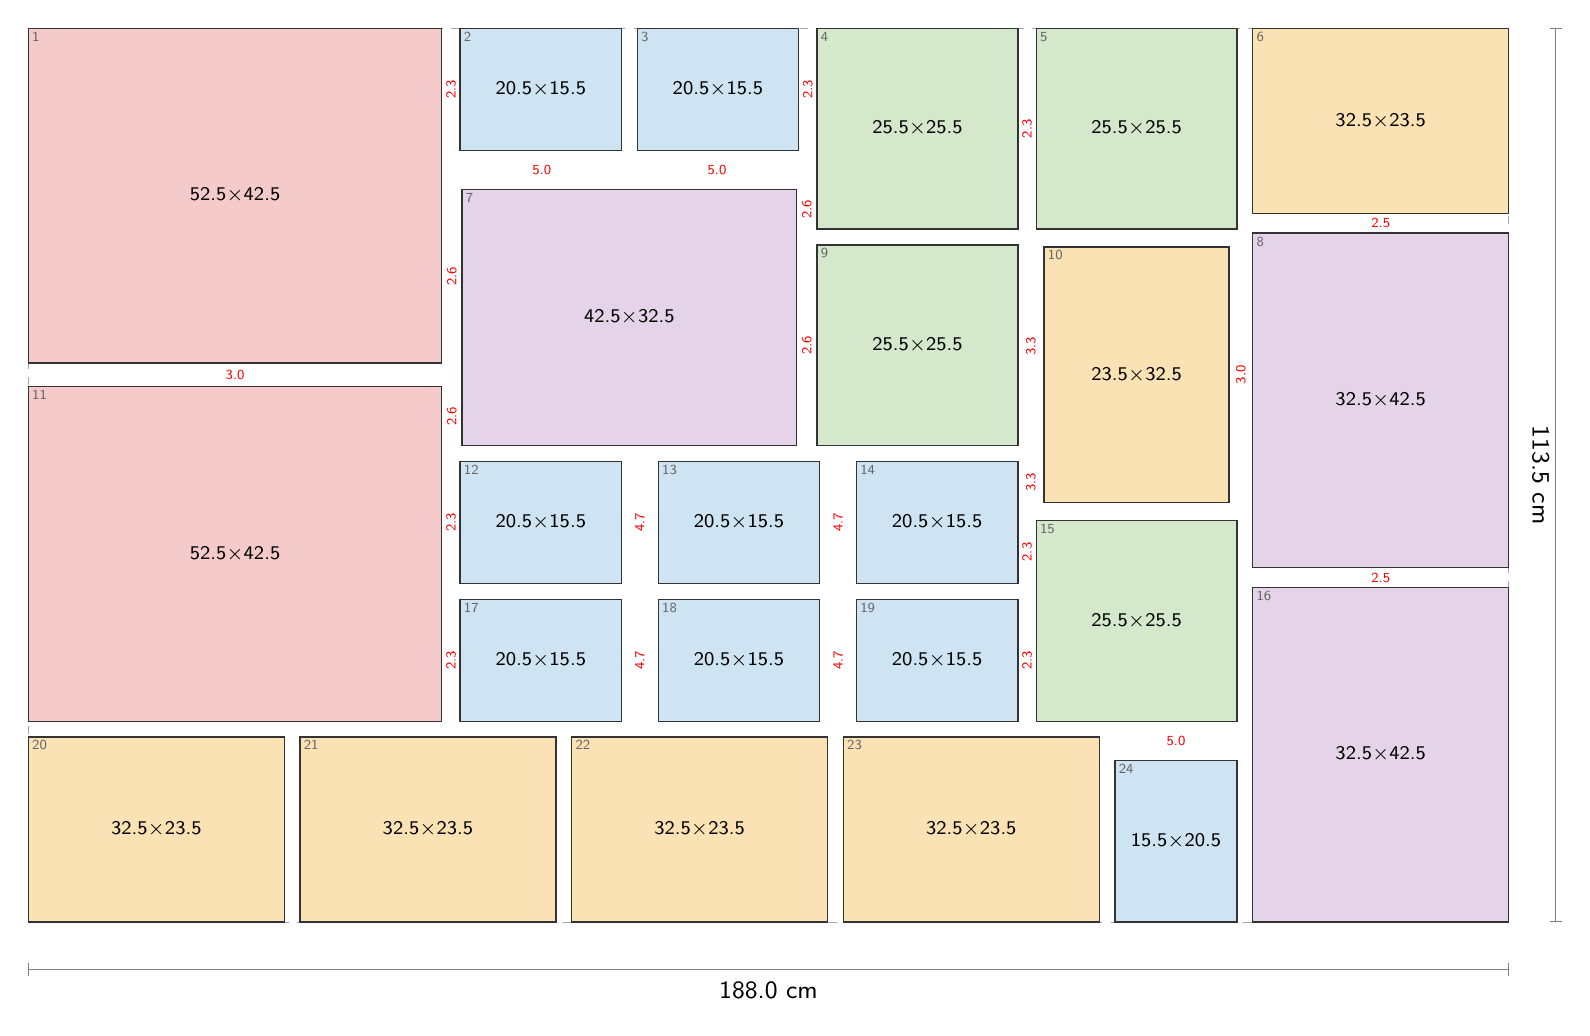
\begin{tikzpicture}[x=1mm, y=-1mm]
\draw[gray!70, dashed, line width=0.4pt] (0,0) rectangle (188.00,113.50);
\filldraw[fill=ft4, draw=black!80, line width=0.5pt] (0.00,0.00) rectangle (52.50,42.50);
\node[align=center, inner sep=0pt] at (26.25,21.25) {\scriptsize 52.5$\times$42.5};
\node[anchor=north west, inner sep=1.2pt, font=\tiny, text=black!60] at (0.00,0.00) {1};
\filldraw[fill=ft0, draw=black!80, line width=0.5pt] (54.83,0.00) rectangle (75.33,15.50);
\node[align=center, inner sep=0pt] at (65.08,7.75) {\scriptsize 20.5$\times$15.5};
\node[anchor=north west, inner sep=1.2pt, font=\tiny, text=black!60] at (54.83,0.00) {2};
\filldraw[fill=ft0, draw=black!80, line width=0.5pt] (77.33,0.00) rectangle (97.83,15.50);
\node[align=center, inner sep=0pt] at (87.58,7.75) {\scriptsize 20.5$\times$15.5};
\node[anchor=north west, inner sep=1.2pt, font=\tiny, text=black!60] at (77.33,0.00) {3};
\filldraw[fill=ft2, draw=black!80, line width=0.5pt] (100.17,0.00) rectangle (125.67,25.50);
\node[align=center, inner sep=0pt] at (112.92,12.75) {\scriptsize 25.5$\times$25.5};
\node[anchor=north west, inner sep=1.2pt, font=\tiny, text=black!60] at (100.17,0.00) {4};
\filldraw[fill=ft2, draw=black!80, line width=0.5pt] (128.00,0.00) rectangle (153.50,25.50);
\node[align=center, inner sep=0pt] at (140.75,12.75) {\scriptsize 25.5$\times$25.5};
\node[anchor=north west, inner sep=1.2pt, font=\tiny, text=black!60] at (128.00,0.00) {5};
\filldraw[fill=ft1, draw=black!80, line width=0.5pt] (155.50,0.00) rectangle (188.00,23.50);
\node[align=center, inner sep=0pt] at (171.75,11.75) {\scriptsize 32.5$\times$23.5};
\node[anchor=north west, inner sep=1.2pt, font=\tiny, text=black!60] at (155.50,0.00) {6};
\filldraw[fill=ft3, draw=black!80, line width=0.5pt] (55.08,20.50) rectangle (97.58,53.00);
\node[align=center, inner sep=0pt] at (76.33,36.75) {\scriptsize 42.5$\times$32.5};
\node[anchor=north west, inner sep=1.2pt, font=\tiny, text=black!60] at (55.08,20.50) {7};
\filldraw[fill=ft3, draw=black!80, line width=0.5pt] (155.50,26.00) rectangle (188.00,68.50);
\node[align=center, inner sep=0pt] at (171.75,47.25) {\scriptsize 32.5$\times$42.5};
\node[anchor=north west, inner sep=1.2pt, font=\tiny, text=black!60] at (155.50,26.00) {8};
\filldraw[fill=ft2, draw=black!80, line width=0.5pt] (100.17,27.50) rectangle (125.67,53.00);
\node[align=center, inner sep=0pt] at (112.92,40.25) {\scriptsize 25.5$\times$25.5};
\node[anchor=north west, inner sep=1.2pt, font=\tiny, text=black!60] at (100.17,27.50) {9};
\filldraw[fill=ft1, draw=black!80, line width=0.5pt] (129.00,27.75) rectangle (152.50,60.25);
\node[align=center, inner sep=0pt] at (140.75,44.00) {\scriptsize 23.5$\times$32.5};
\node[anchor=north west, inner sep=1.2pt, font=\tiny, text=black!60] at (129.00,27.75) {10};
\filldraw[fill=ft4, draw=black!80, line width=0.5pt] (0.00,45.50) rectangle (52.50,88.00);
\node[align=center, inner sep=0pt] at (26.25,66.75) {\scriptsize 52.5$\times$42.5};
\node[anchor=north west, inner sep=1.2pt, font=\tiny, text=black!60] at (0.00,45.50) {11};
\filldraw[fill=ft0, draw=black!80, line width=0.5pt] (54.83,55.00) rectangle (75.33,70.50);
\node[align=center, inner sep=0pt] at (65.08,62.75) {\scriptsize 20.5$\times$15.5};
\node[anchor=north west, inner sep=1.2pt, font=\tiny, text=black!60] at (54.83,55.00) {12};
\filldraw[fill=ft0, draw=black!80, line width=0.5pt] (80.00,55.00) rectangle (100.50,70.50);
\node[align=center, inner sep=0pt] at (90.25,62.75) {\scriptsize 20.5$\times$15.5};
\node[anchor=north west, inner sep=1.2pt, font=\tiny, text=black!60] at (80.00,55.00) {13};
\filldraw[fill=ft0, draw=black!80, line width=0.5pt] (105.17,55.00) rectangle (125.67,70.50);
\node[align=center, inner sep=0pt] at (115.42,62.75) {\scriptsize 20.5$\times$15.5};
\node[anchor=north west, inner sep=1.2pt, font=\tiny, text=black!60] at (105.17,55.00) {14};
\filldraw[fill=ft2, draw=black!80, line width=0.5pt] (128.00,62.50) rectangle (153.50,88.00);
\node[align=center, inner sep=0pt] at (140.75,75.25) {\scriptsize 25.5$\times$25.5};
\node[anchor=north west, inner sep=1.2pt, font=\tiny, text=black!60] at (128.00,62.50) {15};
\filldraw[fill=ft3, draw=black!80, line width=0.5pt] (155.50,71.00) rectangle (188.00,113.50);
\node[align=center, inner sep=0pt] at (171.75,92.25) {\scriptsize 32.5$\times$42.5};
\node[anchor=north west, inner sep=1.2pt, font=\tiny, text=black!60] at (155.50,71.00) {16};
\filldraw[fill=ft0, draw=black!80, line width=0.5pt] (54.83,72.50) rectangle (75.33,88.00);
\node[align=center, inner sep=0pt] at (65.08,80.25) {\scriptsize 20.5$\times$15.5};
\node[anchor=north west, inner sep=1.2pt, font=\tiny, text=black!60] at (54.83,72.50) {17};
\filldraw[fill=ft0, draw=black!80, line width=0.5pt] (80.00,72.50) rectangle (100.50,88.00);
\node[align=center, inner sep=0pt] at (90.25,80.25) {\scriptsize 20.5$\times$15.5};
\node[anchor=north west, inner sep=1.2pt, font=\tiny, text=black!60] at (80.00,72.50) {18};
\filldraw[fill=ft0, draw=black!80, line width=0.5pt] (105.17,72.50) rectangle (125.67,88.00);
\node[align=center, inner sep=0pt] at (115.42,80.25) {\scriptsize 20.5$\times$15.5};
\node[anchor=north west, inner sep=1.2pt, font=\tiny, text=black!60] at (105.17,72.50) {19};
\filldraw[fill=ft1, draw=black!80, line width=0.5pt] (0.00,90.00) rectangle (32.50,113.50);
\node[align=center, inner sep=0pt] at (16.25,101.75) {\scriptsize 32.5$\times$23.5};
\node[anchor=north west, inner sep=1.2pt, font=\tiny, text=black!60] at (0.00,90.00) {20};
\filldraw[fill=ft1, draw=black!80, line width=0.5pt] (34.50,90.00) rectangle (67.00,113.50);
\node[align=center, inner sep=0pt] at (50.75,101.75) {\scriptsize 32.5$\times$23.5};
\node[anchor=north west, inner sep=1.2pt, font=\tiny, text=black!60] at (34.50,90.00) {21};
\filldraw[fill=ft1, draw=black!80, line width=0.5pt] (69.00,90.00) rectangle (101.50,113.50);
\node[align=center, inner sep=0pt] at (85.25,101.75) {\scriptsize 32.5$\times$23.5};
\node[anchor=north west, inner sep=1.2pt, font=\tiny, text=black!60] at (69.00,90.00) {22};
\filldraw[fill=ft1, draw=black!80, line width=0.5pt] (103.50,90.00) rectangle (136.00,113.50);
\node[align=center, inner sep=0pt] at (119.75,101.75) {\scriptsize 32.5$\times$23.5};
\node[anchor=north west, inner sep=1.2pt, font=\tiny, text=black!60] at (103.50,90.00) {23};
\filldraw[fill=ft0, draw=black!80, line width=0.5pt] (138.00,93.00) rectangle (153.50,113.50);
\node[align=center, inner sep=0pt] at (145.75,103.25) {\scriptsize 15.5$\times$20.5};
\node[anchor=north west, inner sep=1.2pt, font=\tiny, text=black!60] at (138.00,93.00) {24};
\node[font=\tiny, text=red, fill=white, inner sep=0.3pt, rotate=90] at (53.67,7.75) {2.3};
\node[font=\tiny, text=red, fill=white, inner sep=0.3pt, rotate=90] at (53.79,31.50) {2.6};
\node[font=\tiny, text=red, fill=white, inner sep=0.3pt] at (26.25,44.00) {3.0};
\node[font=\tiny, text=red, fill=white, inner sep=0.3pt] at (65.21,18.00) {5.0};
\node[font=\tiny, text=red, fill=white, inner sep=0.3pt, rotate=90] at (99.00,7.75) {2.3};
\node[font=\tiny, text=red, fill=white, inner sep=0.3pt] at (87.46,18.00) {5.0};
\node[font=\tiny, text=red, fill=white, inner sep=0.3pt, rotate=90] at (126.83,12.75) {2.3};
\node[font=\tiny, text=red, fill=white, inner sep=0.3pt] at (171.75,24.75) {2.5};
\node[font=\tiny, text=red, fill=white, inner sep=0.3pt, rotate=90] at (98.88,23.00) {2.6};
\node[font=\tiny, text=red, fill=white, inner sep=0.3pt, rotate=90] at (98.88,40.25) {2.6};
\node[font=\tiny, text=red, fill=white, inner sep=0.3pt] at (171.75,69.75) {2.5};
\node[font=\tiny, text=red, fill=white, inner sep=0.3pt, rotate=90] at (127.33,40.38) {3.3};
\node[font=\tiny, text=red, fill=white, inner sep=0.3pt, rotate=90] at (154.00,44.00) {3.0};
\node[font=\tiny, text=red, fill=white, inner sep=0.3pt, rotate=90] at (53.79,49.25) {2.6};
\node[font=\tiny, text=red, fill=white, inner sep=0.3pt, rotate=90] at (53.67,62.75) {2.3};
\node[font=\tiny, text=red, fill=white, inner sep=0.3pt, rotate=90] at (53.67,80.25) {2.3};
\node[font=\tiny, text=red, fill=white, inner sep=0.3pt, rotate=90] at (77.67,62.75) {4.7};
\node[font=\tiny, text=red, fill=white, inner sep=0.3pt, rotate=90] at (102.83,62.75) {4.7};
\node[font=\tiny, text=red, fill=white, inner sep=0.3pt, rotate=90] at (127.33,57.62) {3.3};
\node[font=\tiny, text=red, fill=white, inner sep=0.3pt, rotate=90] at (126.83,66.50) {2.3};
\node[font=\tiny, text=red, fill=white, inner sep=0.3pt] at (145.75,90.50) {5.0};
\node[font=\tiny, text=red, fill=white, inner sep=0.3pt, rotate=90] at (77.67,80.25) {4.7};
\node[font=\tiny, text=red, fill=white, inner sep=0.3pt, rotate=90] at (102.83,80.25) {4.7};
\node[font=\tiny, text=red, fill=white, inner sep=0.3pt, rotate=90] at (126.83,80.25) {2.3};
\draw[Bar-Bar, gray] (0,119.50) -- (188.00,119.50) node[midway, below=1pt, font=\small, text=black] {188.0 cm};
\draw[Bar-Bar, gray] (194.00,0) -- (194.00,113.50) node[midway, right=1pt, font=\small, text=black, rotate=-90, anchor=north] {113.5 cm};
\end{tikzpicture}\\[4pt]
{\scriptsize Scale 1:10 (1 mm = 1 cm). Red numbers mark gaps that deviate from the nominal gap by more than 0.25 cm. Small grey numbers index the coordinate table.}
\end{minipage}\hfill
\begin{minipage}[t]{0.25\textwidth}\vspace{0pt}
\small
\begin{tabular}{@{}l l@{}}
\toprule
Outer size & 188.0 $\times$ 113.5 cm \\
Nominal gap & 2 cm \\
Actual gaps & 2.0 -- 5.0 cm \\
Max.\ deviation & 3.0 cm \\
Mean deviation & 0.62 cm \\
Border notches & none \\
Corners filled & 4 / 4 \\
Frames used & 24 of 28 \\
Large frames & {\scriptsize 2, touching 1$\times$ (52 cm), min.\ dist.\ 46 cm} \\
Entropy & 0.76 \\
\quad {\scriptsize mix / variety} & {\scriptsize 0.82 / 0.72} \\
\quad {\scriptsize stagger / lines} & {\scriptsize 0.51 / 1.00 (1 through)} \\
\bottomrule
\end{tabular}

\vspace{8pt}
\scriptsize
\begin{tabular}{@{}c l l r r@{}}
\toprule
 & outer w $\times$ h (cm) &  & used & have \\
\midrule
\tikz[baseline=-0.6ex]\fill[ft0,draw=black!60] (0,0) rectangle (1.2ex,1.2ex); & 20.5$\times$15.5 & L & 8 & 9 \\
\tikz[baseline=-0.6ex]\fill[ft0,draw=black!60] (0,0) rectangle (1.2ex,1.2ex); & 15.5$\times$20.5 & P & 1 & 2 \\
\tikz[baseline=-0.6ex]\fill[ft3,draw=black!60] (0,0) rectangle (1.2ex,1.2ex); & 32.5$\times$42.5 & P & 2 & 2 \\
\tikz[baseline=-0.6ex]\fill[ft3,draw=black!60] (0,0) rectangle (1.2ex,1.2ex); & 42.5$\times$32.5 & L & 1 & 1 \\
\tikz[baseline=-0.6ex]\fill[ft1,draw=black!60] (0,0) rectangle (1.2ex,1.2ex); & 32.5$\times$23.5 & L & 5 & 5 \\
\tikz[baseline=-0.6ex]\fill[ft1,draw=black!60] (0,0) rectangle (1.2ex,1.2ex); & 23.5$\times$32.5 & P & 1 & 1 \\
\tikz[baseline=-0.6ex]\fill[ft2,draw=black!60] (0,0) rectangle (1.2ex,1.2ex); & 25.5$\times$25.5 &  & 4 & 5 \\
\tikz[baseline=-0.6ex]\fill[ft4,draw=black!60] (0,0) rectangle (1.2ex,1.2ex); & 42.5$\times$52.5 & P & 0 & 1 \\
\tikz[baseline=-0.6ex]\fill[ft4,draw=black!60] (0,0) rectangle (1.2ex,1.2ex); & 52.5$\times$42.5 & L & 2 & 2 \\
\bottomrule
\end{tabular}

\vspace{8pt}
{\bfseries Positions} (top-left corner, cm)\\[2pt]
\tiny
\begin{tabular}{@{}r l r r@{}}
\toprule
\# & frame w $\times$ h & x & y \\
\midrule
1 & 52.5 $\times$ 42.5 & 0.0 & 0.0 \\
2 & 20.5 $\times$ 15.5 & 54.8 & 0.0 \\
3 & 20.5 $\times$ 15.5 & 77.3 & 0.0 \\
4 & 25.5 $\times$ 25.5 & 100.2 & 0.0 \\
5 & 25.5 $\times$ 25.5 & 128.0 & 0.0 \\
6 & 32.5 $\times$ 23.5 & 155.5 & 0.0 \\
7 & 42.5 $\times$ 32.5 & 55.1 & 20.5 \\
8 & 32.5 $\times$ 42.5 & 155.5 & 26.0 \\
9 & 25.5 $\times$ 25.5 & 100.2 & 27.5 \\
10 & 23.5 $\times$ 32.5 & 129.0 & 27.8 \\
11 & 52.5 $\times$ 42.5 & 0.0 & 45.5 \\
12 & 20.5 $\times$ 15.5 & 54.8 & 55.0 \\
13 & 20.5 $\times$ 15.5 & 80.0 & 55.0 \\
14 & 20.5 $\times$ 15.5 & 105.2 & 55.0 \\
15 & 25.5 $\times$ 25.5 & 128.0 & 62.5 \\
16 & 32.5 $\times$ 42.5 & 155.5 & 71.0 \\
17 & 20.5 $\times$ 15.5 & 54.8 & 72.5 \\
18 & 20.5 $\times$ 15.5 & 80.0 & 72.5 \\
19 & 20.5 $\times$ 15.5 & 105.2 & 72.5 \\
20 & 32.5 $\times$ 23.5 & 0.0 & 90.0 \\
21 & 32.5 $\times$ 23.5 & 34.5 & 90.0 \\
22 & 32.5 $\times$ 23.5 & 69.0 & 90.0 \\
23 & 32.5 $\times$ 23.5 & 103.5 & 90.0 \\
24 & 15.5 $\times$ 20.5 & 138.0 & 93.0 \\
\bottomrule
\end{tabular}
\end{minipage}
\clearpage

\phantomsection\addcontentsline{toc}{subsection}{Layout 2: 167.5 \texorpdfstring{$\times$}{x} 130.5 cm, 24 frames, gap 3.5 cm, max.\ deviation 3.0 cm}
\label{lay:per-run-gap:2}
\begin{minipage}[t]{0.74\textwidth}\vspace{0pt}
{\LARGE\bfseries Layout 2}\hspace{1.5em}{\large 167.5 $\times$ 130.5 cm \quad gap 3.5 cm \quad 24 frames}\\[8pt]
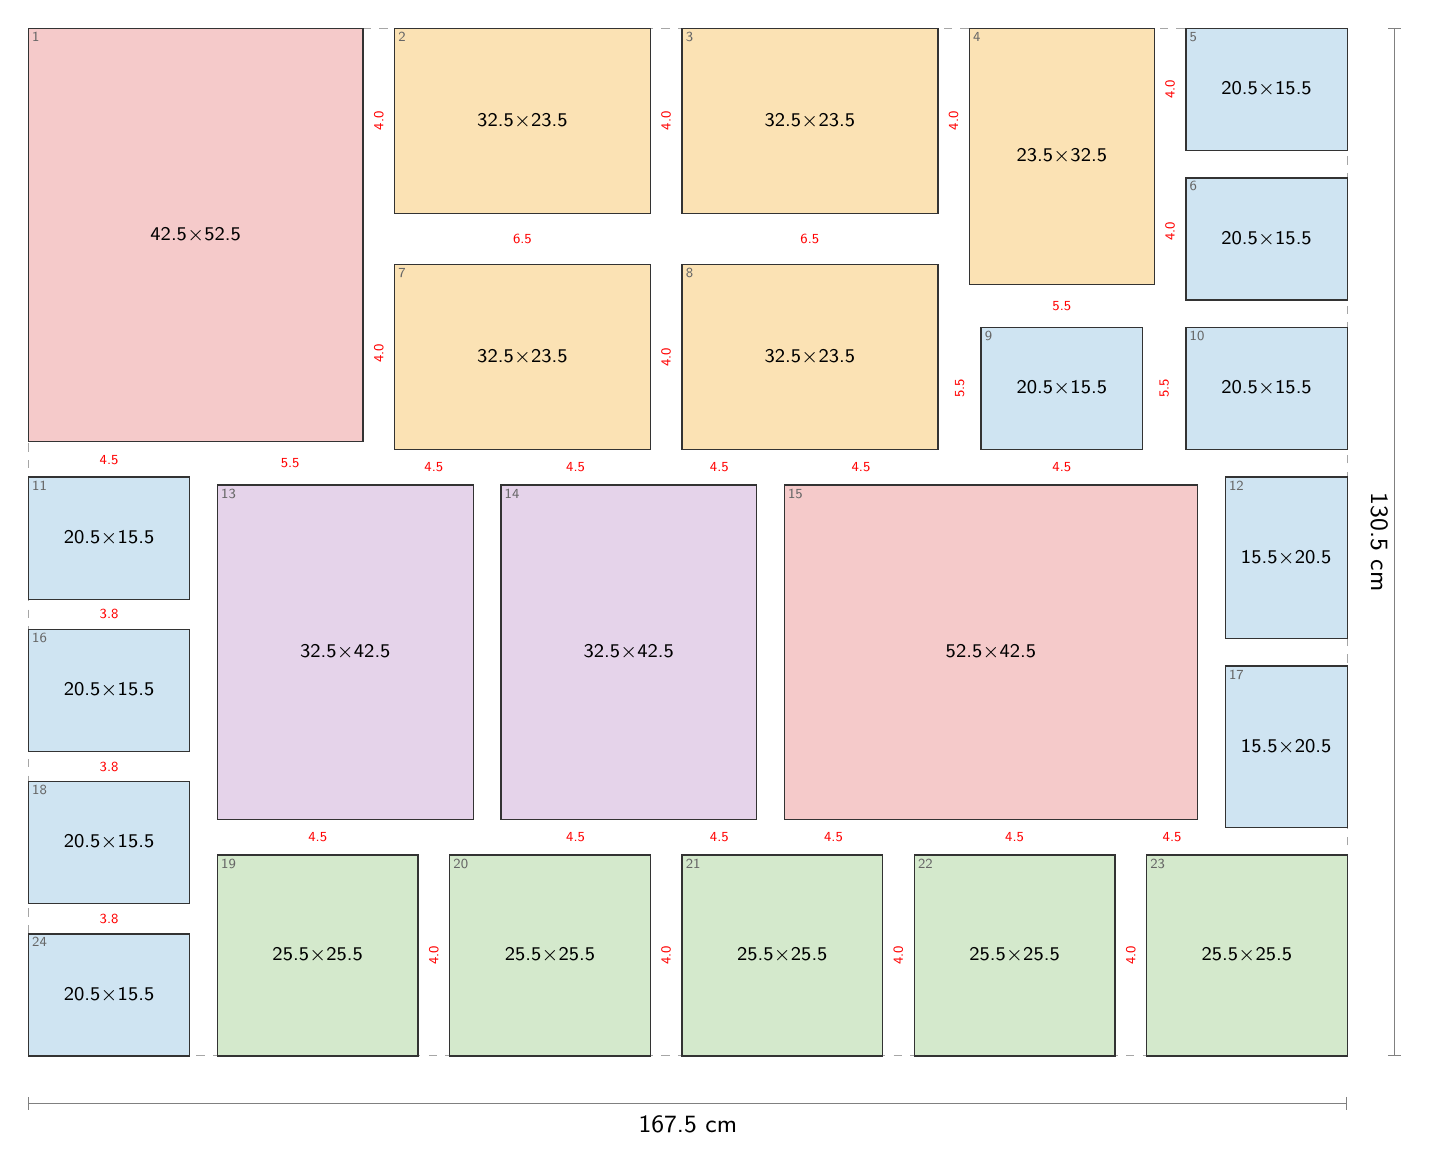
\begin{tikzpicture}[x=1mm, y=-1mm]
\draw[gray!70, dashed, line width=0.4pt] (0,0) rectangle (167.50,130.50);
\filldraw[fill=ft4, draw=black!80, line width=0.5pt] (0.00,0.00) rectangle (42.50,52.50);
\node[align=center, inner sep=0pt] at (21.25,26.25) {\scriptsize 42.5$\times$52.5};
\node[anchor=north west, inner sep=1.2pt, font=\tiny, text=black!60] at (0.00,0.00) {1};
\filldraw[fill=ft1, draw=black!80, line width=0.5pt] (46.50,0.00) rectangle (79.00,23.50);
\node[align=center, inner sep=0pt] at (62.75,11.75) {\scriptsize 32.5$\times$23.5};
\node[anchor=north west, inner sep=1.2pt, font=\tiny, text=black!60] at (46.50,0.00) {2};
\filldraw[fill=ft1, draw=black!80, line width=0.5pt] (83.00,0.00) rectangle (115.50,23.50);
\node[align=center, inner sep=0pt] at (99.25,11.75) {\scriptsize 32.5$\times$23.5};
\node[anchor=north west, inner sep=1.2pt, font=\tiny, text=black!60] at (83.00,0.00) {3};
\filldraw[fill=ft1, draw=black!80, line width=0.5pt] (119.50,0.00) rectangle (143.00,32.50);
\node[align=center, inner sep=0pt] at (131.25,16.25) {\scriptsize 23.5$\times$32.5};
\node[anchor=north west, inner sep=1.2pt, font=\tiny, text=black!60] at (119.50,0.00) {4};
\filldraw[fill=ft0, draw=black!80, line width=0.5pt] (147.00,0.00) rectangle (167.50,15.50);
\node[align=center, inner sep=0pt] at (157.25,7.75) {\scriptsize 20.5$\times$15.5};
\node[anchor=north west, inner sep=1.2pt, font=\tiny, text=black!60] at (147.00,0.00) {5};
\filldraw[fill=ft0, draw=black!80, line width=0.5pt] (147.00,19.00) rectangle (167.50,34.50);
\node[align=center, inner sep=0pt] at (157.25,26.75) {\scriptsize 20.5$\times$15.5};
\node[anchor=north west, inner sep=1.2pt, font=\tiny, text=black!60] at (147.00,19.00) {6};
\filldraw[fill=ft1, draw=black!80, line width=0.5pt] (46.50,30.00) rectangle (79.00,53.50);
\node[align=center, inner sep=0pt] at (62.75,41.75) {\scriptsize 32.5$\times$23.5};
\node[anchor=north west, inner sep=1.2pt, font=\tiny, text=black!60] at (46.50,30.00) {7};
\filldraw[fill=ft1, draw=black!80, line width=0.5pt] (83.00,30.00) rectangle (115.50,53.50);
\node[align=center, inner sep=0pt] at (99.25,41.75) {\scriptsize 32.5$\times$23.5};
\node[anchor=north west, inner sep=1.2pt, font=\tiny, text=black!60] at (83.00,30.00) {8};
\filldraw[fill=ft0, draw=black!80, line width=0.5pt] (121.00,38.00) rectangle (141.50,53.50);
\node[align=center, inner sep=0pt] at (131.25,45.75) {\scriptsize 20.5$\times$15.5};
\node[anchor=north west, inner sep=1.2pt, font=\tiny, text=black!60] at (121.00,38.00) {9};
\filldraw[fill=ft0, draw=black!80, line width=0.5pt] (147.00,38.00) rectangle (167.50,53.50);
\node[align=center, inner sep=0pt] at (157.25,45.75) {\scriptsize 20.5$\times$15.5};
\node[anchor=north west, inner sep=1.2pt, font=\tiny, text=black!60] at (147.00,38.00) {10};
\filldraw[fill=ft0, draw=black!80, line width=0.5pt] (0.00,57.00) rectangle (20.50,72.50);
\node[align=center, inner sep=0pt] at (10.25,64.75) {\scriptsize 20.5$\times$15.5};
\node[anchor=north west, inner sep=1.2pt, font=\tiny, text=black!60] at (0.00,57.00) {11};
\filldraw[fill=ft0, draw=black!80, line width=0.5pt] (152.00,57.00) rectangle (167.50,77.50);
\node[align=center, inner sep=0pt] at (159.75,67.25) {\scriptsize 15.5$\times$20.5};
\node[anchor=north west, inner sep=1.2pt, font=\tiny, text=black!60] at (152.00,57.00) {12};
\filldraw[fill=ft3, draw=black!80, line width=0.5pt] (24.00,58.00) rectangle (56.50,100.50);
\node[align=center, inner sep=0pt] at (40.25,79.25) {\scriptsize 32.5$\times$42.5};
\node[anchor=north west, inner sep=1.2pt, font=\tiny, text=black!60] at (24.00,58.00) {13};
\filldraw[fill=ft3, draw=black!80, line width=0.5pt] (60.00,58.00) rectangle (92.50,100.50);
\node[align=center, inner sep=0pt] at (76.25,79.25) {\scriptsize 32.5$\times$42.5};
\node[anchor=north west, inner sep=1.2pt, font=\tiny, text=black!60] at (60.00,58.00) {14};
\filldraw[fill=ft4, draw=black!80, line width=0.5pt] (96.00,58.00) rectangle (148.50,100.50);
\node[align=center, inner sep=0pt] at (122.25,79.25) {\scriptsize 52.5$\times$42.5};
\node[anchor=north west, inner sep=1.2pt, font=\tiny, text=black!60] at (96.00,58.00) {15};
\filldraw[fill=ft0, draw=black!80, line width=0.5pt] (0.00,76.33) rectangle (20.50,91.83);
\node[align=center, inner sep=0pt] at (10.25,84.08) {\scriptsize 20.5$\times$15.5};
\node[anchor=north west, inner sep=1.2pt, font=\tiny, text=black!60] at (0.00,76.33) {16};
\filldraw[fill=ft0, draw=black!80, line width=0.5pt] (152.00,81.00) rectangle (167.50,101.50);
\node[align=center, inner sep=0pt] at (159.75,91.25) {\scriptsize 15.5$\times$20.5};
\node[anchor=north west, inner sep=1.2pt, font=\tiny, text=black!60] at (152.00,81.00) {17};
\filldraw[fill=ft0, draw=black!80, line width=0.5pt] (0.00,95.67) rectangle (20.50,111.17);
\node[align=center, inner sep=0pt] at (10.25,103.42) {\scriptsize 20.5$\times$15.5};
\node[anchor=north west, inner sep=1.2pt, font=\tiny, text=black!60] at (0.00,95.67) {18};
\filldraw[fill=ft2, draw=black!80, line width=0.5pt] (24.00,105.00) rectangle (49.50,130.50);
\node[align=center, inner sep=0pt] at (36.75,117.75) {\scriptsize 25.5$\times$25.5};
\node[anchor=north west, inner sep=1.2pt, font=\tiny, text=black!60] at (24.00,105.00) {19};
\filldraw[fill=ft2, draw=black!80, line width=0.5pt] (53.50,105.00) rectangle (79.00,130.50);
\node[align=center, inner sep=0pt] at (66.25,117.75) {\scriptsize 25.5$\times$25.5};
\node[anchor=north west, inner sep=1.2pt, font=\tiny, text=black!60] at (53.50,105.00) {20};
\filldraw[fill=ft2, draw=black!80, line width=0.5pt] (83.00,105.00) rectangle (108.50,130.50);
\node[align=center, inner sep=0pt] at (95.75,117.75) {\scriptsize 25.5$\times$25.5};
\node[anchor=north west, inner sep=1.2pt, font=\tiny, text=black!60] at (83.00,105.00) {21};
\filldraw[fill=ft2, draw=black!80, line width=0.5pt] (112.50,105.00) rectangle (138.00,130.50);
\node[align=center, inner sep=0pt] at (125.25,117.75) {\scriptsize 25.5$\times$25.5};
\node[anchor=north west, inner sep=1.2pt, font=\tiny, text=black!60] at (112.50,105.00) {22};
\filldraw[fill=ft2, draw=black!80, line width=0.5pt] (142.00,105.00) rectangle (167.50,130.50);
\node[align=center, inner sep=0pt] at (154.75,117.75) {\scriptsize 25.5$\times$25.5};
\node[anchor=north west, inner sep=1.2pt, font=\tiny, text=black!60] at (142.00,105.00) {23};
\filldraw[fill=ft0, draw=black!80, line width=0.5pt] (0.00,115.00) rectangle (20.50,130.50);
\node[align=center, inner sep=0pt] at (10.25,122.75) {\scriptsize 20.5$\times$15.5};
\node[anchor=north west, inner sep=1.2pt, font=\tiny, text=black!60] at (0.00,115.00) {24};
\node[font=\tiny, text=red, fill=white, inner sep=0.3pt, rotate=90] at (44.50,11.75) {4.0};
\node[font=\tiny, text=red, fill=white, inner sep=0.3pt, rotate=90] at (44.50,41.25) {4.0};
\node[font=\tiny, text=red, fill=white, inner sep=0.3pt] at (10.25,54.75) {4.5};
\node[font=\tiny, text=red, fill=white, inner sep=0.3pt] at (33.25,55.25) {5.5};
\node[font=\tiny, text=red, fill=white, inner sep=0.3pt, rotate=90] at (81.00,11.75) {4.0};
\node[font=\tiny, text=red, fill=white, inner sep=0.3pt] at (62.75,26.75) {6.5};
\node[font=\tiny, text=red, fill=white, inner sep=0.3pt, rotate=90] at (117.50,11.75) {4.0};
\node[font=\tiny, text=red, fill=white, inner sep=0.3pt] at (99.25,26.75) {6.5};
\node[font=\tiny, text=red, fill=white, inner sep=0.3pt, rotate=90] at (145.00,7.75) {4.0};
\node[font=\tiny, text=red, fill=white, inner sep=0.3pt, rotate=90] at (145.00,25.75) {4.0};
\node[font=\tiny, text=red, fill=white, inner sep=0.3pt] at (131.25,35.25) {5.5};
\node[font=\tiny, text=red, fill=white, inner sep=0.3pt, rotate=90] at (81.00,41.75) {4.0};
\node[font=\tiny, text=red, fill=white, inner sep=0.3pt] at (51.50,55.75) {4.5};
\node[font=\tiny, text=red, fill=white, inner sep=0.3pt] at (69.50,55.75) {4.5};
\node[font=\tiny, text=red, fill=white, inner sep=0.3pt, rotate=90] at (118.25,45.75) {5.5};
\node[font=\tiny, text=red, fill=white, inner sep=0.3pt] at (87.75,55.75) {4.5};
\node[font=\tiny, text=red, fill=white, inner sep=0.3pt] at (105.75,55.75) {4.5};
\node[font=\tiny, text=red, fill=white, inner sep=0.3pt, rotate=90] at (144.25,45.75) {5.5};
\node[font=\tiny, text=red, fill=white, inner sep=0.3pt] at (131.25,55.75) {4.5};
\node[font=\tiny, text=red, fill=white, inner sep=0.3pt] at (10.25,74.42) {3.8};
\node[font=\tiny, text=red, fill=white, inner sep=0.3pt] at (36.75,102.75) {4.5};
\node[font=\tiny, text=red, fill=white, inner sep=0.3pt] at (69.50,102.75) {4.5};
\node[font=\tiny, text=red, fill=white, inner sep=0.3pt] at (87.75,102.75) {4.5};
\node[font=\tiny, text=red, fill=white, inner sep=0.3pt] at (102.25,102.75) {4.5};
\node[font=\tiny, text=red, fill=white, inner sep=0.3pt] at (125.25,102.75) {4.5};
\node[font=\tiny, text=red, fill=white, inner sep=0.3pt] at (145.25,102.75) {4.5};
\node[font=\tiny, text=red, fill=white, inner sep=0.3pt] at (10.25,93.75) {3.8};
\node[font=\tiny, text=red, fill=white, inner sep=0.3pt] at (10.25,113.08) {3.8};
\node[font=\tiny, text=red, fill=white, inner sep=0.3pt, rotate=90] at (51.50,117.75) {4.0};
\node[font=\tiny, text=red, fill=white, inner sep=0.3pt, rotate=90] at (81.00,117.75) {4.0};
\node[font=\tiny, text=red, fill=white, inner sep=0.3pt, rotate=90] at (110.50,117.75) {4.0};
\node[font=\tiny, text=red, fill=white, inner sep=0.3pt, rotate=90] at (140.00,117.75) {4.0};
\draw[Bar-Bar, gray] (0,136.50) -- (167.50,136.50) node[midway, below=1pt, font=\small, text=black] {167.5 cm};
\draw[Bar-Bar, gray] (173.50,0) -- (173.50,130.50) node[midway, right=1pt, font=\small, text=black, rotate=-90, anchor=north] {130.5 cm};
\end{tikzpicture}\\[4pt]
{\scriptsize Scale 1:10 (1 mm = 1 cm). Red numbers mark gaps that deviate from the nominal gap by more than 0.25 cm. Small grey numbers index the coordinate table.}
\end{minipage}\hfill
\begin{minipage}[t]{0.25\textwidth}\vspace{0pt}
\small
\begin{tabular}{@{}l l@{}}
\toprule
Outer size & 167.5 $\times$ 130.5 cm \\
Nominal gap & 3.5 cm \\
Actual gaps & 3.5 -- 6.5 cm \\
Max.\ deviation & 3.0 cm \\
Mean deviation & 0.72 cm \\
Border notches & none \\
Corners filled & 4 / 4 \\
Frames used & 24 of 28 \\
Large frames & {\scriptsize 2, not touching, min.\ dist.\ 114 cm} \\
Entropy & 0.75 \\
\quad {\scriptsize mix / variety} & {\scriptsize 0.82 / 0.67} \\
\quad {\scriptsize stagger / lines} & {\scriptsize 0.52 / 1.00 (1 through)} \\
\bottomrule
\end{tabular}

\vspace{8pt}
\scriptsize
\begin{tabular}{@{}c l l r r@{}}
\toprule
 & outer w $\times$ h (cm) &  & used & have \\
\midrule
\tikz[baseline=-0.6ex]\fill[ft0,draw=black!60] (0,0) rectangle (1.2ex,1.2ex); & 20.5$\times$15.5 & L & 8 & 9 \\
\tikz[baseline=-0.6ex]\fill[ft0,draw=black!60] (0,0) rectangle (1.2ex,1.2ex); & 15.5$\times$20.5 & P & 2 & 2 \\
\tikz[baseline=-0.6ex]\fill[ft3,draw=black!60] (0,0) rectangle (1.2ex,1.2ex); & 32.5$\times$42.5 & P & 2 & 2 \\
\tikz[baseline=-0.6ex]\fill[ft3,draw=black!60] (0,0) rectangle (1.2ex,1.2ex); & 42.5$\times$32.5 & L & 0 & 1 \\
\tikz[baseline=-0.6ex]\fill[ft1,draw=black!60] (0,0) rectangle (1.2ex,1.2ex); & 32.5$\times$23.5 & L & 4 & 5 \\
\tikz[baseline=-0.6ex]\fill[ft1,draw=black!60] (0,0) rectangle (1.2ex,1.2ex); & 23.5$\times$32.5 & P & 1 & 1 \\
\tikz[baseline=-0.6ex]\fill[ft2,draw=black!60] (0,0) rectangle (1.2ex,1.2ex); & 25.5$\times$25.5 &  & 5 & 5 \\
\tikz[baseline=-0.6ex]\fill[ft4,draw=black!60] (0,0) rectangle (1.2ex,1.2ex); & 42.5$\times$52.5 & P & 1 & 1 \\
\tikz[baseline=-0.6ex]\fill[ft4,draw=black!60] (0,0) rectangle (1.2ex,1.2ex); & 52.5$\times$42.5 & L & 1 & 2 \\
\bottomrule
\end{tabular}

\vspace{8pt}
{\bfseries Positions} (top-left corner, cm)\\[2pt]
\tiny
\begin{tabular}{@{}r l r r@{}}
\toprule
\# & frame w $\times$ h & x & y \\
\midrule
1 & 42.5 $\times$ 52.5 & 0.0 & 0.0 \\
2 & 32.5 $\times$ 23.5 & 46.5 & 0.0 \\
3 & 32.5 $\times$ 23.5 & 83.0 & 0.0 \\
4 & 23.5 $\times$ 32.5 & 119.5 & 0.0 \\
5 & 20.5 $\times$ 15.5 & 147.0 & 0.0 \\
6 & 20.5 $\times$ 15.5 & 147.0 & 19.0 \\
7 & 32.5 $\times$ 23.5 & 46.5 & 30.0 \\
8 & 32.5 $\times$ 23.5 & 83.0 & 30.0 \\
9 & 20.5 $\times$ 15.5 & 121.0 & 38.0 \\
10 & 20.5 $\times$ 15.5 & 147.0 & 38.0 \\
11 & 20.5 $\times$ 15.5 & 0.0 & 57.0 \\
12 & 15.5 $\times$ 20.5 & 152.0 & 57.0 \\
13 & 32.5 $\times$ 42.5 & 24.0 & 58.0 \\
14 & 32.5 $\times$ 42.5 & 60.0 & 58.0 \\
15 & 52.5 $\times$ 42.5 & 96.0 & 58.0 \\
16 & 20.5 $\times$ 15.5 & 0.0 & 76.3 \\
17 & 15.5 $\times$ 20.5 & 152.0 & 81.0 \\
18 & 20.5 $\times$ 15.5 & 0.0 & 95.7 \\
19 & 25.5 $\times$ 25.5 & 24.0 & 105.0 \\
20 & 25.5 $\times$ 25.5 & 53.5 & 105.0 \\
21 & 25.5 $\times$ 25.5 & 83.0 & 105.0 \\
22 & 25.5 $\times$ 25.5 & 112.5 & 105.0 \\
23 & 25.5 $\times$ 25.5 & 142.0 & 105.0 \\
24 & 20.5 $\times$ 15.5 & 0.0 & 115.0 \\
\bottomrule
\end{tabular}
\end{minipage}
\clearpage

\phantomsection\addcontentsline{toc}{subsection}{Layout 3: 183.5 \texorpdfstring{$\times$}{x} 115.0 cm, 23 frames, gap 2 cm, max.\ deviation 2.2 cm}
\label{lay:per-run-gap:3}
\begin{minipage}[t]{0.74\textwidth}\vspace{0pt}
{\LARGE\bfseries Layout 3}\hspace{1.5em}{\large 183.5 $\times$ 115.0 cm \quad gap 2 cm \quad 23 frames}\\[8pt]
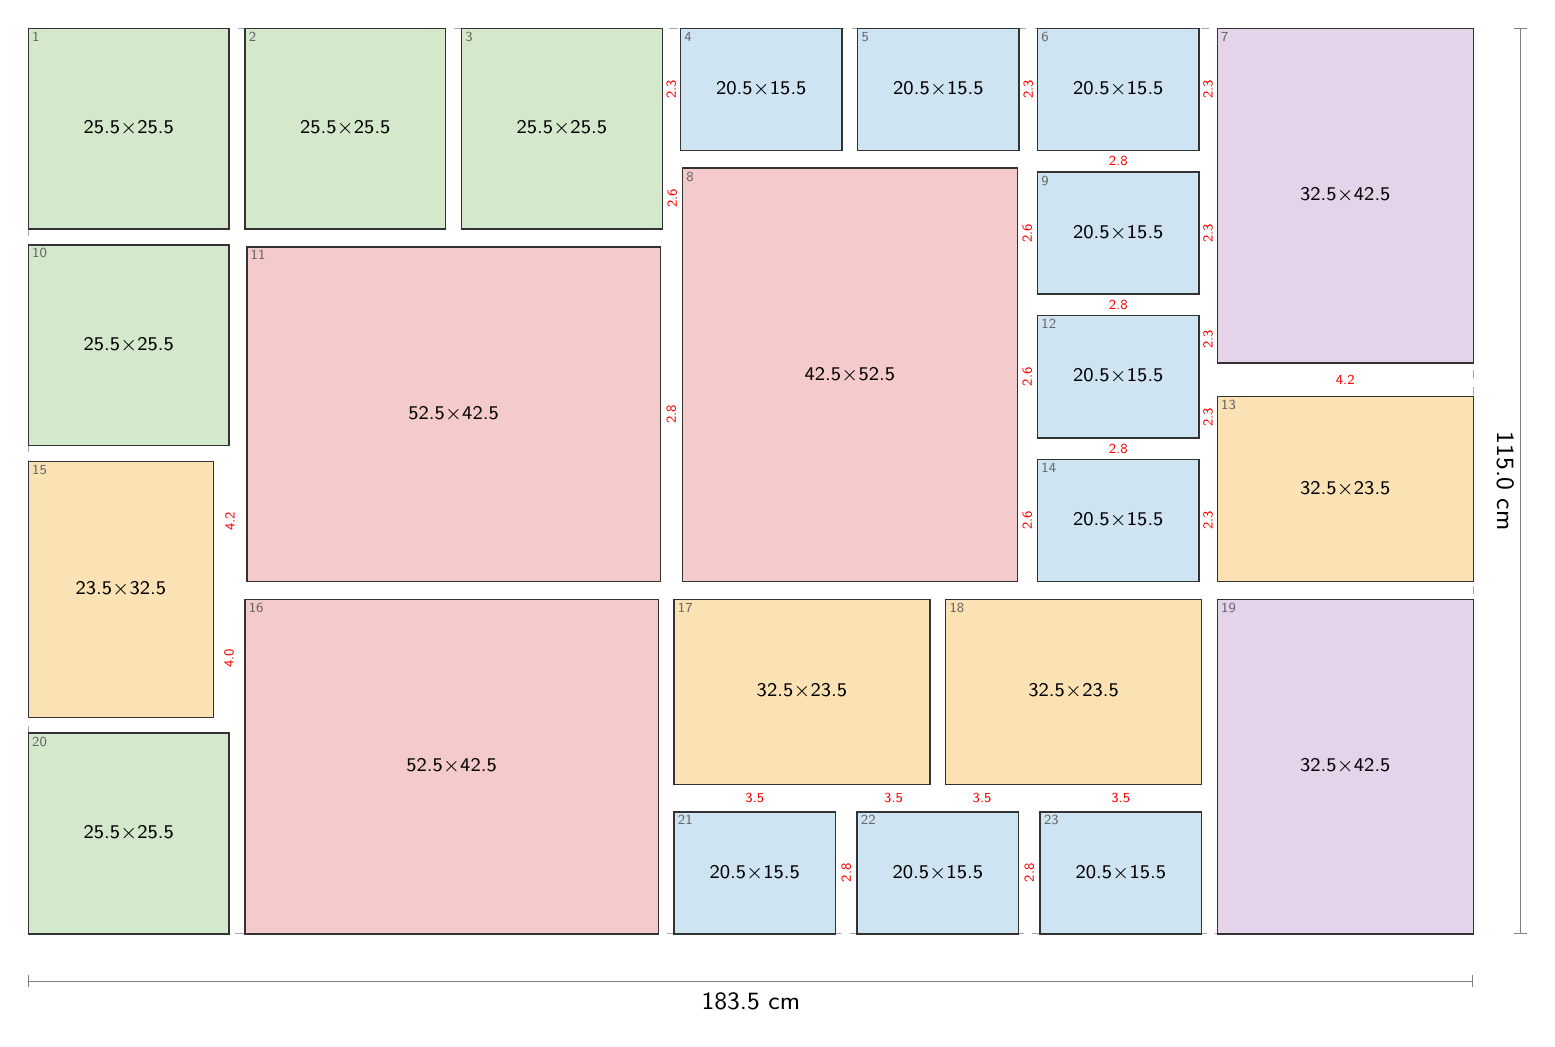
\begin{tikzpicture}[x=1mm, y=-1mm]
\draw[gray!70, dashed, line width=0.4pt] (0,0) rectangle (183.50,115.00);
\filldraw[fill=ft2, draw=black!80, line width=0.5pt] (0.00,0.00) rectangle (25.50,25.50);
\node[align=center, inner sep=0pt] at (12.75,12.75) {\scriptsize 25.5$\times$25.5};
\node[anchor=north west, inner sep=1.2pt, font=\tiny, text=black!60] at (0.00,0.00) {1};
\filldraw[fill=ft2, draw=black!80, line width=0.5pt] (27.50,0.00) rectangle (53.00,25.50);
\node[align=center, inner sep=0pt] at (40.25,12.75) {\scriptsize 25.5$\times$25.5};
\node[anchor=north west, inner sep=1.2pt, font=\tiny, text=black!60] at (27.50,0.00) {2};
\filldraw[fill=ft2, draw=black!80, line width=0.5pt] (55.00,0.00) rectangle (80.50,25.50);
\node[align=center, inner sep=0pt] at (67.75,12.75) {\scriptsize 25.5$\times$25.5};
\node[anchor=north west, inner sep=1.2pt, font=\tiny, text=black!60] at (55.00,0.00) {3};
\filldraw[fill=ft0, draw=black!80, line width=0.5pt] (82.83,0.00) rectangle (103.33,15.50);
\node[align=center, inner sep=0pt] at (93.08,7.75) {\scriptsize 20.5$\times$15.5};
\node[anchor=north west, inner sep=1.2pt, font=\tiny, text=black!60] at (82.83,0.00) {4};
\filldraw[fill=ft0, draw=black!80, line width=0.5pt] (105.33,0.00) rectangle (125.83,15.50);
\node[align=center, inner sep=0pt] at (115.58,7.75) {\scriptsize 20.5$\times$15.5};
\node[anchor=north west, inner sep=1.2pt, font=\tiny, text=black!60] at (105.33,0.00) {5};
\filldraw[fill=ft0, draw=black!80, line width=0.5pt] (128.17,0.00) rectangle (148.67,15.50);
\node[align=center, inner sep=0pt] at (138.42,7.75) {\scriptsize 20.5$\times$15.5};
\node[anchor=north west, inner sep=1.2pt, font=\tiny, text=black!60] at (128.17,0.00) {6};
\filldraw[fill=ft3, draw=black!80, line width=0.5pt] (151.00,0.00) rectangle (183.50,42.50);
\node[align=center, inner sep=0pt] at (167.25,21.25) {\scriptsize 32.5$\times$42.5};
\node[anchor=north west, inner sep=1.2pt, font=\tiny, text=black!60] at (151.00,0.00) {7};
\filldraw[fill=ft4, draw=black!80, line width=0.5pt] (83.08,17.75) rectangle (125.58,70.25);
\node[align=center, inner sep=0pt] at (104.33,44.00) {\scriptsize 42.5$\times$52.5};
\node[anchor=north west, inner sep=1.2pt, font=\tiny, text=black!60] at (83.08,17.75) {8};
\filldraw[fill=ft0, draw=black!80, line width=0.5pt] (128.17,18.25) rectangle (148.67,33.75);
\node[align=center, inner sep=0pt] at (138.42,26.00) {\scriptsize 20.5$\times$15.5};
\node[anchor=north west, inner sep=1.2pt, font=\tiny, text=black!60] at (128.17,18.25) {9};
\filldraw[fill=ft2, draw=black!80, line width=0.5pt] (0.00,27.50) rectangle (25.50,53.00);
\node[align=center, inner sep=0pt] at (12.75,40.25) {\scriptsize 25.5$\times$25.5};
\node[anchor=north west, inner sep=1.2pt, font=\tiny, text=black!60] at (0.00,27.50) {10};
\filldraw[fill=ft4, draw=black!80, line width=0.5pt] (27.75,27.75) rectangle (80.25,70.25);
\node[align=center, inner sep=0pt] at (54.00,49.00) {\scriptsize 52.5$\times$42.5};
\node[anchor=north west, inner sep=1.2pt, font=\tiny, text=black!60] at (27.75,27.75) {11};
\filldraw[fill=ft0, draw=black!80, line width=0.5pt] (128.17,36.50) rectangle (148.67,52.00);
\node[align=center, inner sep=0pt] at (138.42,44.25) {\scriptsize 20.5$\times$15.5};
\node[anchor=north west, inner sep=1.2pt, font=\tiny, text=black!60] at (128.17,36.50) {12};
\filldraw[fill=ft1, draw=black!80, line width=0.5pt] (151.00,46.75) rectangle (183.50,70.25);
\node[align=center, inner sep=0pt] at (167.25,58.50) {\scriptsize 32.5$\times$23.5};
\node[anchor=north west, inner sep=1.2pt, font=\tiny, text=black!60] at (151.00,46.75) {13};
\filldraw[fill=ft0, draw=black!80, line width=0.5pt] (128.17,54.75) rectangle (148.67,70.25);
\node[align=center, inner sep=0pt] at (138.42,62.50) {\scriptsize 20.5$\times$15.5};
\node[anchor=north west, inner sep=1.2pt, font=\tiny, text=black!60] at (128.17,54.75) {14};
\filldraw[fill=ft1, draw=black!80, line width=0.5pt] (0.00,55.00) rectangle (23.50,87.50);
\node[align=center, inner sep=0pt] at (11.75,71.25) {\scriptsize 23.5$\times$32.5};
\node[anchor=north west, inner sep=1.2pt, font=\tiny, text=black!60] at (0.00,55.00) {15};
\filldraw[fill=ft4, draw=black!80, line width=0.5pt] (27.50,72.50) rectangle (80.00,115.00);
\node[align=center, inner sep=0pt] at (53.75,93.75) {\scriptsize 52.5$\times$42.5};
\node[anchor=north west, inner sep=1.2pt, font=\tiny, text=black!60] at (27.50,72.50) {16};
\filldraw[fill=ft1, draw=black!80, line width=0.5pt] (82.00,72.50) rectangle (114.50,96.00);
\node[align=center, inner sep=0pt] at (98.25,84.25) {\scriptsize 32.5$\times$23.5};
\node[anchor=north west, inner sep=1.2pt, font=\tiny, text=black!60] at (82.00,72.50) {17};
\filldraw[fill=ft1, draw=black!80, line width=0.5pt] (116.50,72.50) rectangle (149.00,96.00);
\node[align=center, inner sep=0pt] at (132.75,84.25) {\scriptsize 32.5$\times$23.5};
\node[anchor=north west, inner sep=1.2pt, font=\tiny, text=black!60] at (116.50,72.50) {18};
\filldraw[fill=ft3, draw=black!80, line width=0.5pt] (151.00,72.50) rectangle (183.50,115.00);
\node[align=center, inner sep=0pt] at (167.25,93.75) {\scriptsize 32.5$\times$42.5};
\node[anchor=north west, inner sep=1.2pt, font=\tiny, text=black!60] at (151.00,72.50) {19};
\filldraw[fill=ft2, draw=black!80, line width=0.5pt] (0.00,89.50) rectangle (25.50,115.00);
\node[align=center, inner sep=0pt] at (12.75,102.25) {\scriptsize 25.5$\times$25.5};
\node[anchor=north west, inner sep=1.2pt, font=\tiny, text=black!60] at (0.00,89.50) {20};
\filldraw[fill=ft0, draw=black!80, line width=0.5pt] (82.00,99.50) rectangle (102.50,115.00);
\node[align=center, inner sep=0pt] at (92.25,107.25) {\scriptsize 20.5$\times$15.5};
\node[anchor=north west, inner sep=1.2pt, font=\tiny, text=black!60] at (82.00,99.50) {21};
\filldraw[fill=ft0, draw=black!80, line width=0.5pt] (105.25,99.50) rectangle (125.75,115.00);
\node[align=center, inner sep=0pt] at (115.50,107.25) {\scriptsize 20.5$\times$15.5};
\node[anchor=north west, inner sep=1.2pt, font=\tiny, text=black!60] at (105.25,99.50) {22};
\filldraw[fill=ft0, draw=black!80, line width=0.5pt] (128.50,99.50) rectangle (149.00,115.00);
\node[align=center, inner sep=0pt] at (138.75,107.25) {\scriptsize 20.5$\times$15.5};
\node[anchor=north west, inner sep=1.2pt, font=\tiny, text=black!60] at (128.50,99.50) {23};
\node[font=\tiny, text=red, fill=white, inner sep=0.3pt, rotate=90] at (81.67,7.75) {2.3};
\node[font=\tiny, text=red, fill=white, inner sep=0.3pt, rotate=90] at (81.79,21.62) {2.6};
\node[font=\tiny, text=red, fill=white, inner sep=0.3pt, rotate=90] at (127.00,7.75) {2.3};
\node[font=\tiny, text=red, fill=white, inner sep=0.3pt, rotate=90] at (149.83,7.75) {2.3};
\node[font=\tiny, text=red, fill=white, inner sep=0.3pt] at (138.42,16.88) {2.8};
\node[font=\tiny, text=red, fill=white, inner sep=0.3pt] at (167.25,44.62) {4.2};
\node[font=\tiny, text=red, fill=white, inner sep=0.3pt, rotate=90] at (126.88,26.00) {2.6};
\node[font=\tiny, text=red, fill=white, inner sep=0.3pt, rotate=90] at (126.88,44.25) {2.6};
\node[font=\tiny, text=red, fill=white, inner sep=0.3pt, rotate=90] at (126.88,62.50) {2.6};
\node[font=\tiny, text=red, fill=white, inner sep=0.3pt, rotate=90] at (149.83,26.00) {2.3};
\node[font=\tiny, text=red, fill=white, inner sep=0.3pt] at (138.42,35.12) {2.8};
\node[font=\tiny, text=red, fill=white, inner sep=0.3pt, rotate=90] at (81.67,49.00) {2.8};
\node[font=\tiny, text=red, fill=white, inner sep=0.3pt, rotate=90] at (149.83,39.50) {2.3};
\node[font=\tiny, text=red, fill=white, inner sep=0.3pt, rotate=90] at (149.83,49.38) {2.3};
\node[font=\tiny, text=red, fill=white, inner sep=0.3pt] at (138.42,53.38) {2.8};
\node[font=\tiny, text=red, fill=white, inner sep=0.3pt, rotate=90] at (149.83,62.50) {2.3};
\node[font=\tiny, text=red, fill=white, inner sep=0.3pt, rotate=90] at (25.62,62.62) {4.2};
\node[font=\tiny, text=red, fill=white, inner sep=0.3pt, rotate=90] at (25.50,80.00) {4.0};
\node[font=\tiny, text=red, fill=white, inner sep=0.3pt] at (92.25,97.75) {3.5};
\node[font=\tiny, text=red, fill=white, inner sep=0.3pt] at (109.88,97.75) {3.5};
\node[font=\tiny, text=red, fill=white, inner sep=0.3pt] at (121.12,97.75) {3.5};
\node[font=\tiny, text=red, fill=white, inner sep=0.3pt] at (138.75,97.75) {3.5};
\node[font=\tiny, text=red, fill=white, inner sep=0.3pt, rotate=90] at (103.88,107.25) {2.8};
\node[font=\tiny, text=red, fill=white, inner sep=0.3pt, rotate=90] at (127.12,107.25) {2.8};
\draw[Bar-Bar, gray] (0,121.00) -- (183.50,121.00) node[midway, below=1pt, font=\small, text=black] {183.5 cm};
\draw[Bar-Bar, gray] (189.50,0) -- (189.50,115.00) node[midway, right=1pt, font=\small, text=black, rotate=-90, anchor=north] {115.0 cm};
\end{tikzpicture}\\[4pt]
{\scriptsize Scale 1:10 (1 mm = 1 cm). Red numbers mark gaps that deviate from the nominal gap by more than 0.25 cm. Small grey numbers index the coordinate table.}
\end{minipage}\hfill
\begin{minipage}[t]{0.25\textwidth}\vspace{0pt}
\small
\begin{tabular}{@{}l l@{}}
\toprule
Outer size & 183.5 $\times$ 115.0 cm \\
Nominal gap & 2 cm \\
Actual gaps & 2.0 -- 4.2 cm \\
Max.\ deviation & 2.2 cm \\
Mean deviation & 0.53 cm \\
Border notches & right 4 cm \\
Corners filled & 4 / 4 \\
Frames used & 23 of 28 \\
Large frames & {\scriptsize 3, touching 2$\times$ (95 cm), min.\ dist.\ 45 cm} \\
Entropy & 0.62 \\
\quad {\scriptsize mix / variety} & {\scriptsize 0.76 / 0.69} \\
\quad {\scriptsize stagger / lines} & {\scriptsize 0.53 / 0.50 (3 through)} \\
\bottomrule
\end{tabular}

\vspace{8pt}
\scriptsize
\begin{tabular}{@{}c l l r r@{}}
\toprule
 & outer w $\times$ h (cm) &  & used & have \\
\midrule
\tikz[baseline=-0.6ex]\fill[ft0,draw=black!60] (0,0) rectangle (1.2ex,1.2ex); & 20.5$\times$15.5 & L & 9 & 9 \\
\tikz[baseline=-0.6ex]\fill[ft0,draw=black!60] (0,0) rectangle (1.2ex,1.2ex); & 15.5$\times$20.5 & P & 0 & 2 \\
\tikz[baseline=-0.6ex]\fill[ft3,draw=black!60] (0,0) rectangle (1.2ex,1.2ex); & 32.5$\times$42.5 & P & 2 & 2 \\
\tikz[baseline=-0.6ex]\fill[ft3,draw=black!60] (0,0) rectangle (1.2ex,1.2ex); & 42.5$\times$32.5 & L & 0 & 1 \\
\tikz[baseline=-0.6ex]\fill[ft1,draw=black!60] (0,0) rectangle (1.2ex,1.2ex); & 32.5$\times$23.5 & L & 3 & 5 \\
\tikz[baseline=-0.6ex]\fill[ft1,draw=black!60] (0,0) rectangle (1.2ex,1.2ex); & 23.5$\times$32.5 & P & 1 & 1 \\
\tikz[baseline=-0.6ex]\fill[ft2,draw=black!60] (0,0) rectangle (1.2ex,1.2ex); & 25.5$\times$25.5 &  & 5 & 5 \\
\tikz[baseline=-0.6ex]\fill[ft4,draw=black!60] (0,0) rectangle (1.2ex,1.2ex); & 42.5$\times$52.5 & P & 1 & 1 \\
\tikz[baseline=-0.6ex]\fill[ft4,draw=black!60] (0,0) rectangle (1.2ex,1.2ex); & 52.5$\times$42.5 & L & 2 & 2 \\
\bottomrule
\end{tabular}

\vspace{8pt}
{\bfseries Positions} (top-left corner, cm)\\[2pt]
\tiny
\begin{tabular}{@{}r l r r@{}}
\toprule
\# & frame w $\times$ h & x & y \\
\midrule
1 & 25.5 $\times$ 25.5 & 0.0 & 0.0 \\
2 & 25.5 $\times$ 25.5 & 27.5 & 0.0 \\
3 & 25.5 $\times$ 25.5 & 55.0 & 0.0 \\
4 & 20.5 $\times$ 15.5 & 82.8 & 0.0 \\
5 & 20.5 $\times$ 15.5 & 105.3 & 0.0 \\
6 & 20.5 $\times$ 15.5 & 128.2 & 0.0 \\
7 & 32.5 $\times$ 42.5 & 151.0 & 0.0 \\
8 & 42.5 $\times$ 52.5 & 83.1 & 17.8 \\
9 & 20.5 $\times$ 15.5 & 128.2 & 18.2 \\
10 & 25.5 $\times$ 25.5 & 0.0 & 27.5 \\
11 & 52.5 $\times$ 42.5 & 27.8 & 27.8 \\
12 & 20.5 $\times$ 15.5 & 128.2 & 36.5 \\
13 & 32.5 $\times$ 23.5 & 151.0 & 46.8 \\
14 & 20.5 $\times$ 15.5 & 128.2 & 54.8 \\
15 & 23.5 $\times$ 32.5 & 0.0 & 55.0 \\
16 & 52.5 $\times$ 42.5 & 27.5 & 72.5 \\
17 & 32.5 $\times$ 23.5 & 82.0 & 72.5 \\
18 & 32.5 $\times$ 23.5 & 116.5 & 72.5 \\
19 & 32.5 $\times$ 42.5 & 151.0 & 72.5 \\
20 & 25.5 $\times$ 25.5 & 0.0 & 89.5 \\
21 & 20.5 $\times$ 15.5 & 82.0 & 99.5 \\
22 & 20.5 $\times$ 15.5 & 105.2 & 99.5 \\
23 & 20.5 $\times$ 15.5 & 128.5 & 99.5 \\
\bottomrule
\end{tabular}
\end{minipage}
\clearpage

\phantomsection\addcontentsline{toc}{subsection}{Layout 4: 169.5 \texorpdfstring{$\times$}{x} 117.5 cm, 21 frames, gap 4.5 cm, max.\ deviation 3.0 cm}
\label{lay:per-run-gap:4}
\begin{minipage}[t]{0.74\textwidth}\vspace{0pt}
{\LARGE\bfseries Layout 4}\hspace{1.5em}{\large 169.5 $\times$ 117.5 cm \quad gap 4.5 cm \quad 21 frames}\\[8pt]
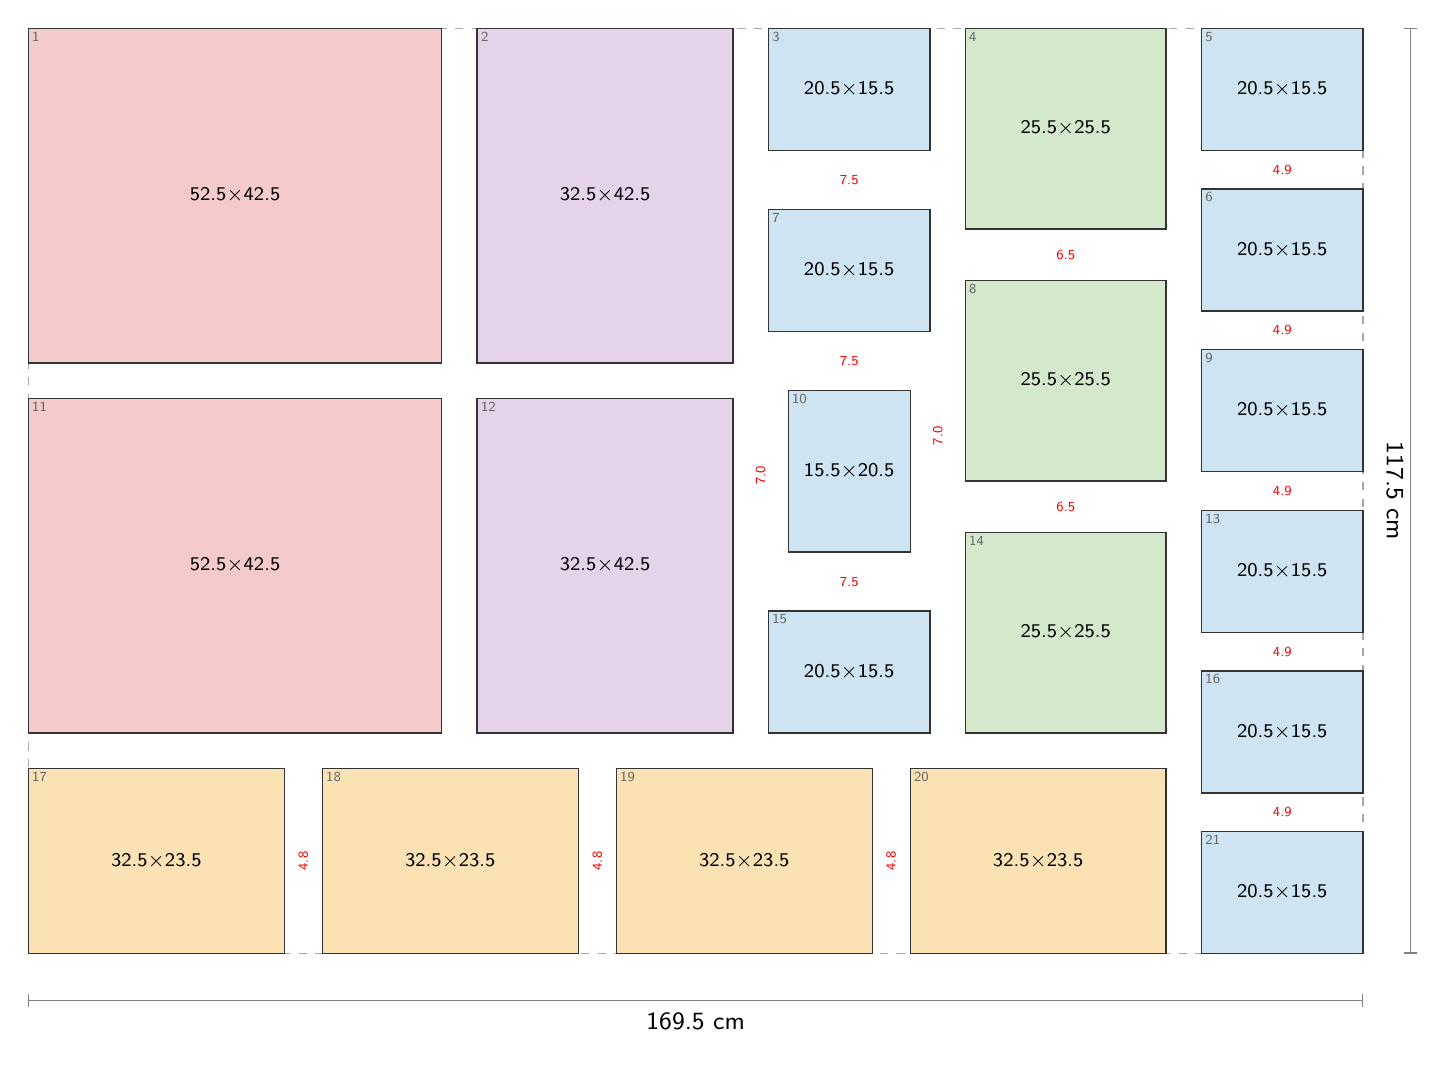
\begin{tikzpicture}[x=1mm, y=-1mm]
\draw[gray!70, dashed, line width=0.4pt] (0,0) rectangle (169.50,117.50);
\filldraw[fill=ft4, draw=black!80, line width=0.5pt] (0.00,0.00) rectangle (52.50,42.50);
\node[align=center, inner sep=0pt] at (26.25,21.25) {\scriptsize 52.5$\times$42.5};
\node[anchor=north west, inner sep=1.2pt, font=\tiny, text=black!60] at (0.00,0.00) {1};
\filldraw[fill=ft3, draw=black!80, line width=0.5pt] (57.00,0.00) rectangle (89.50,42.50);
\node[align=center, inner sep=0pt] at (73.25,21.25) {\scriptsize 32.5$\times$42.5};
\node[anchor=north west, inner sep=1.2pt, font=\tiny, text=black!60] at (57.00,0.00) {2};
\filldraw[fill=ft0, draw=black!80, line width=0.5pt] (94.00,0.00) rectangle (114.50,15.50);
\node[align=center, inner sep=0pt] at (104.25,7.75) {\scriptsize 20.5$\times$15.5};
\node[anchor=north west, inner sep=1.2pt, font=\tiny, text=black!60] at (94.00,0.00) {3};
\filldraw[fill=ft2, draw=black!80, line width=0.5pt] (119.00,0.00) rectangle (144.50,25.50);
\node[align=center, inner sep=0pt] at (131.75,12.75) {\scriptsize 25.5$\times$25.5};
\node[anchor=north west, inner sep=1.2pt, font=\tiny, text=black!60] at (119.00,0.00) {4};
\filldraw[fill=ft0, draw=black!80, line width=0.5pt] (149.00,0.00) rectangle (169.50,15.50);
\node[align=center, inner sep=0pt] at (159.25,7.75) {\scriptsize 20.5$\times$15.5};
\node[anchor=north west, inner sep=1.2pt, font=\tiny, text=black!60] at (149.00,0.00) {5};
\filldraw[fill=ft0, draw=black!80, line width=0.5pt] (149.00,20.40) rectangle (169.50,35.90);
\node[align=center, inner sep=0pt] at (159.25,28.15) {\scriptsize 20.5$\times$15.5};
\node[anchor=north west, inner sep=1.2pt, font=\tiny, text=black!60] at (149.00,20.40) {6};
\filldraw[fill=ft0, draw=black!80, line width=0.5pt] (94.00,23.00) rectangle (114.50,38.50);
\node[align=center, inner sep=0pt] at (104.25,30.75) {\scriptsize 20.5$\times$15.5};
\node[anchor=north west, inner sep=1.2pt, font=\tiny, text=black!60] at (94.00,23.00) {7};
\filldraw[fill=ft2, draw=black!80, line width=0.5pt] (119.00,32.00) rectangle (144.50,57.50);
\node[align=center, inner sep=0pt] at (131.75,44.75) {\scriptsize 25.5$\times$25.5};
\node[anchor=north west, inner sep=1.2pt, font=\tiny, text=black!60] at (119.00,32.00) {8};
\filldraw[fill=ft0, draw=black!80, line width=0.5pt] (149.00,40.80) rectangle (169.50,56.30);
\node[align=center, inner sep=0pt] at (159.25,48.55) {\scriptsize 20.5$\times$15.5};
\node[anchor=north west, inner sep=1.2pt, font=\tiny, text=black!60] at (149.00,40.80) {9};
\filldraw[fill=ft0, draw=black!80, line width=0.5pt] (96.50,46.00) rectangle (112.00,66.50);
\node[align=center, inner sep=0pt] at (104.25,56.25) {\scriptsize 15.5$\times$20.5};
\node[anchor=north west, inner sep=1.2pt, font=\tiny, text=black!60] at (96.50,46.00) {10};
\filldraw[fill=ft4, draw=black!80, line width=0.5pt] (0.00,47.00) rectangle (52.50,89.50);
\node[align=center, inner sep=0pt] at (26.25,68.25) {\scriptsize 52.5$\times$42.5};
\node[anchor=north west, inner sep=1.2pt, font=\tiny, text=black!60] at (0.00,47.00) {11};
\filldraw[fill=ft3, draw=black!80, line width=0.5pt] (57.00,47.00) rectangle (89.50,89.50);
\node[align=center, inner sep=0pt] at (73.25,68.25) {\scriptsize 32.5$\times$42.5};
\node[anchor=north west, inner sep=1.2pt, font=\tiny, text=black!60] at (57.00,47.00) {12};
\filldraw[fill=ft0, draw=black!80, line width=0.5pt] (149.00,61.20) rectangle (169.50,76.70);
\node[align=center, inner sep=0pt] at (159.25,68.95) {\scriptsize 20.5$\times$15.5};
\node[anchor=north west, inner sep=1.2pt, font=\tiny, text=black!60] at (149.00,61.20) {13};
\filldraw[fill=ft2, draw=black!80, line width=0.5pt] (119.00,64.00) rectangle (144.50,89.50);
\node[align=center, inner sep=0pt] at (131.75,76.75) {\scriptsize 25.5$\times$25.5};
\node[anchor=north west, inner sep=1.2pt, font=\tiny, text=black!60] at (119.00,64.00) {14};
\filldraw[fill=ft0, draw=black!80, line width=0.5pt] (94.00,74.00) rectangle (114.50,89.50);
\node[align=center, inner sep=0pt] at (104.25,81.75) {\scriptsize 20.5$\times$15.5};
\node[anchor=north west, inner sep=1.2pt, font=\tiny, text=black!60] at (94.00,74.00) {15};
\filldraw[fill=ft0, draw=black!80, line width=0.5pt] (149.00,81.60) rectangle (169.50,97.10);
\node[align=center, inner sep=0pt] at (159.25,89.35) {\scriptsize 20.5$\times$15.5};
\node[anchor=north west, inner sep=1.2pt, font=\tiny, text=black!60] at (149.00,81.60) {16};
\filldraw[fill=ft1, draw=black!80, line width=0.5pt] (0.00,94.00) rectangle (32.50,117.50);
\node[align=center, inner sep=0pt] at (16.25,105.75) {\scriptsize 32.5$\times$23.5};
\node[anchor=north west, inner sep=1.2pt, font=\tiny, text=black!60] at (0.00,94.00) {17};
\filldraw[fill=ft1, draw=black!80, line width=0.5pt] (37.33,94.00) rectangle (69.83,117.50);
\node[align=center, inner sep=0pt] at (53.58,105.75) {\scriptsize 32.5$\times$23.5};
\node[anchor=north west, inner sep=1.2pt, font=\tiny, text=black!60] at (37.33,94.00) {18};
\filldraw[fill=ft1, draw=black!80, line width=0.5pt] (74.67,94.00) rectangle (107.17,117.50);
\node[align=center, inner sep=0pt] at (90.92,105.75) {\scriptsize 32.5$\times$23.5};
\node[anchor=north west, inner sep=1.2pt, font=\tiny, text=black!60] at (74.67,94.00) {19};
\filldraw[fill=ft1, draw=black!80, line width=0.5pt] (112.00,94.00) rectangle (144.50,117.50);
\node[align=center, inner sep=0pt] at (128.25,105.75) {\scriptsize 32.5$\times$23.5};
\node[anchor=north west, inner sep=1.2pt, font=\tiny, text=black!60] at (112.00,94.00) {20};
\filldraw[fill=ft0, draw=black!80, line width=0.5pt] (149.00,102.00) rectangle (169.50,117.50);
\node[align=center, inner sep=0pt] at (159.25,109.75) {\scriptsize 20.5$\times$15.5};
\node[anchor=north west, inner sep=1.2pt, font=\tiny, text=black!60] at (149.00,102.00) {21};
\node[font=\tiny, text=red, fill=white, inner sep=0.3pt] at (104.25,19.25) {7.5};
\node[font=\tiny, text=red, fill=white, inner sep=0.3pt] at (131.75,28.75) {6.5};
\node[font=\tiny, text=red, fill=white, inner sep=0.3pt] at (159.25,17.95) {4.9};
\node[font=\tiny, text=red, fill=white, inner sep=0.3pt] at (159.25,38.35) {4.9};
\node[font=\tiny, text=red, fill=white, inner sep=0.3pt] at (104.25,42.25) {7.5};
\node[font=\tiny, text=red, fill=white, inner sep=0.3pt] at (131.75,60.75) {6.5};
\node[font=\tiny, text=red, fill=white, inner sep=0.3pt] at (159.25,58.75) {4.9};
\node[font=\tiny, text=red, fill=white, inner sep=0.3pt, rotate=90] at (115.50,51.75) {7.0};
\node[font=\tiny, text=red, fill=white, inner sep=0.3pt] at (104.25,70.25) {7.5};
\node[font=\tiny, text=red, fill=white, inner sep=0.3pt, rotate=90] at (93.00,56.75) {7.0};
\node[font=\tiny, text=red, fill=white, inner sep=0.3pt] at (159.25,79.15) {4.9};
\node[font=\tiny, text=red, fill=white, inner sep=0.3pt] at (159.25,99.55) {4.9};
\node[font=\tiny, text=red, fill=white, inner sep=0.3pt, rotate=90] at (34.92,105.75) {4.8};
\node[font=\tiny, text=red, fill=white, inner sep=0.3pt, rotate=90] at (72.25,105.75) {4.8};
\node[font=\tiny, text=red, fill=white, inner sep=0.3pt, rotate=90] at (109.58,105.75) {4.8};
\draw[Bar-Bar, gray] (0,123.50) -- (169.50,123.50) node[midway, below=1pt, font=\small, text=black] {169.5 cm};
\draw[Bar-Bar, gray] (175.50,0) -- (175.50,117.50) node[midway, right=1pt, font=\small, text=black, rotate=-90, anchor=north] {117.5 cm};
\end{tikzpicture}\\[4pt]
{\scriptsize Scale 1:10 (1 mm = 1 cm). Red numbers mark gaps that deviate from the nominal gap by more than 0.25 cm. Small grey numbers index the coordinate table.}
\end{minipage}\hfill
\begin{minipage}[t]{0.25\textwidth}\vspace{0pt}
\small
\begin{tabular}{@{}l l@{}}
\toprule
Outer size & 169.5 $\times$ 117.5 cm \\
Nominal gap & 4.5 cm \\
Actual gaps & 4.5 -- 7.5 cm \\
Max.\ deviation & 3.0 cm \\
Mean deviation & 0.57 cm \\
Border notches & none \\
Corners filled & 4 / 4 \\
Frames used & 21 of 28 \\
Large frames & {\scriptsize 2, touching 1$\times$ (52 cm), min.\ dist.\ 47 cm} \\
Entropy & 0.72 \\
\quad {\scriptsize mix / variety} & {\scriptsize 0.71 / 0.67} \\
\quad {\scriptsize stagger / lines} & {\scriptsize 0.50 / 1.00 (1 through)} \\
\bottomrule
\end{tabular}

\vspace{8pt}
\scriptsize
\begin{tabular}{@{}c l l r r@{}}
\toprule
 & outer w $\times$ h (cm) &  & used & have \\
\midrule
\tikz[baseline=-0.6ex]\fill[ft0,draw=black!60] (0,0) rectangle (1.2ex,1.2ex); & 20.5$\times$15.5 & L & 9 & 9 \\
\tikz[baseline=-0.6ex]\fill[ft0,draw=black!60] (0,0) rectangle (1.2ex,1.2ex); & 15.5$\times$20.5 & P & 1 & 2 \\
\tikz[baseline=-0.6ex]\fill[ft3,draw=black!60] (0,0) rectangle (1.2ex,1.2ex); & 32.5$\times$42.5 & P & 2 & 2 \\
\tikz[baseline=-0.6ex]\fill[ft3,draw=black!60] (0,0) rectangle (1.2ex,1.2ex); & 42.5$\times$32.5 & L & 0 & 1 \\
\tikz[baseline=-0.6ex]\fill[ft1,draw=black!60] (0,0) rectangle (1.2ex,1.2ex); & 32.5$\times$23.5 & L & 4 & 5 \\
\tikz[baseline=-0.6ex]\fill[ft1,draw=black!60] (0,0) rectangle (1.2ex,1.2ex); & 23.5$\times$32.5 & P & 0 & 1 \\
\tikz[baseline=-0.6ex]\fill[ft2,draw=black!60] (0,0) rectangle (1.2ex,1.2ex); & 25.5$\times$25.5 &  & 3 & 5 \\
\tikz[baseline=-0.6ex]\fill[ft4,draw=black!60] (0,0) rectangle (1.2ex,1.2ex); & 42.5$\times$52.5 & P & 0 & 1 \\
\tikz[baseline=-0.6ex]\fill[ft4,draw=black!60] (0,0) rectangle (1.2ex,1.2ex); & 52.5$\times$42.5 & L & 2 & 2 \\
\bottomrule
\end{tabular}

\vspace{8pt}
{\bfseries Positions} (top-left corner, cm)\\[2pt]
\tiny
\begin{tabular}{@{}r l r r@{}}
\toprule
\# & frame w $\times$ h & x & y \\
\midrule
1 & 52.5 $\times$ 42.5 & 0.0 & 0.0 \\
2 & 32.5 $\times$ 42.5 & 57.0 & 0.0 \\
3 & 20.5 $\times$ 15.5 & 94.0 & 0.0 \\
4 & 25.5 $\times$ 25.5 & 119.0 & 0.0 \\
5 & 20.5 $\times$ 15.5 & 149.0 & 0.0 \\
6 & 20.5 $\times$ 15.5 & 149.0 & 20.4 \\
7 & 20.5 $\times$ 15.5 & 94.0 & 23.0 \\
8 & 25.5 $\times$ 25.5 & 119.0 & 32.0 \\
9 & 20.5 $\times$ 15.5 & 149.0 & 40.8 \\
10 & 15.5 $\times$ 20.5 & 96.5 & 46.0 \\
11 & 52.5 $\times$ 42.5 & 0.0 & 47.0 \\
12 & 32.5 $\times$ 42.5 & 57.0 & 47.0 \\
13 & 20.5 $\times$ 15.5 & 149.0 & 61.2 \\
14 & 25.5 $\times$ 25.5 & 119.0 & 64.0 \\
15 & 20.5 $\times$ 15.5 & 94.0 & 74.0 \\
16 & 20.5 $\times$ 15.5 & 149.0 & 81.6 \\
17 & 32.5 $\times$ 23.5 & 0.0 & 94.0 \\
18 & 32.5 $\times$ 23.5 & 37.3 & 94.0 \\
19 & 32.5 $\times$ 23.5 & 74.7 & 94.0 \\
20 & 32.5 $\times$ 23.5 & 112.0 & 94.0 \\
21 & 20.5 $\times$ 15.5 & 149.0 & 102.0 \\
\bottomrule
\end{tabular}
\end{minipage}
\clearpage

\phantomsection\addcontentsline{toc}{subsection}{Layout 5: 179.5 \texorpdfstring{$\times$}{x} 123.5 cm, 25 frames, gap 2 cm, max.\ deviation 2.5 cm}
\label{lay:per-run-gap:5}
\begin{minipage}[t]{0.74\textwidth}\vspace{0pt}
{\LARGE\bfseries Layout 5}\hspace{1.5em}{\large 179.5 $\times$ 123.5 cm \quad gap 2 cm \quad 25 frames}\\[8pt]
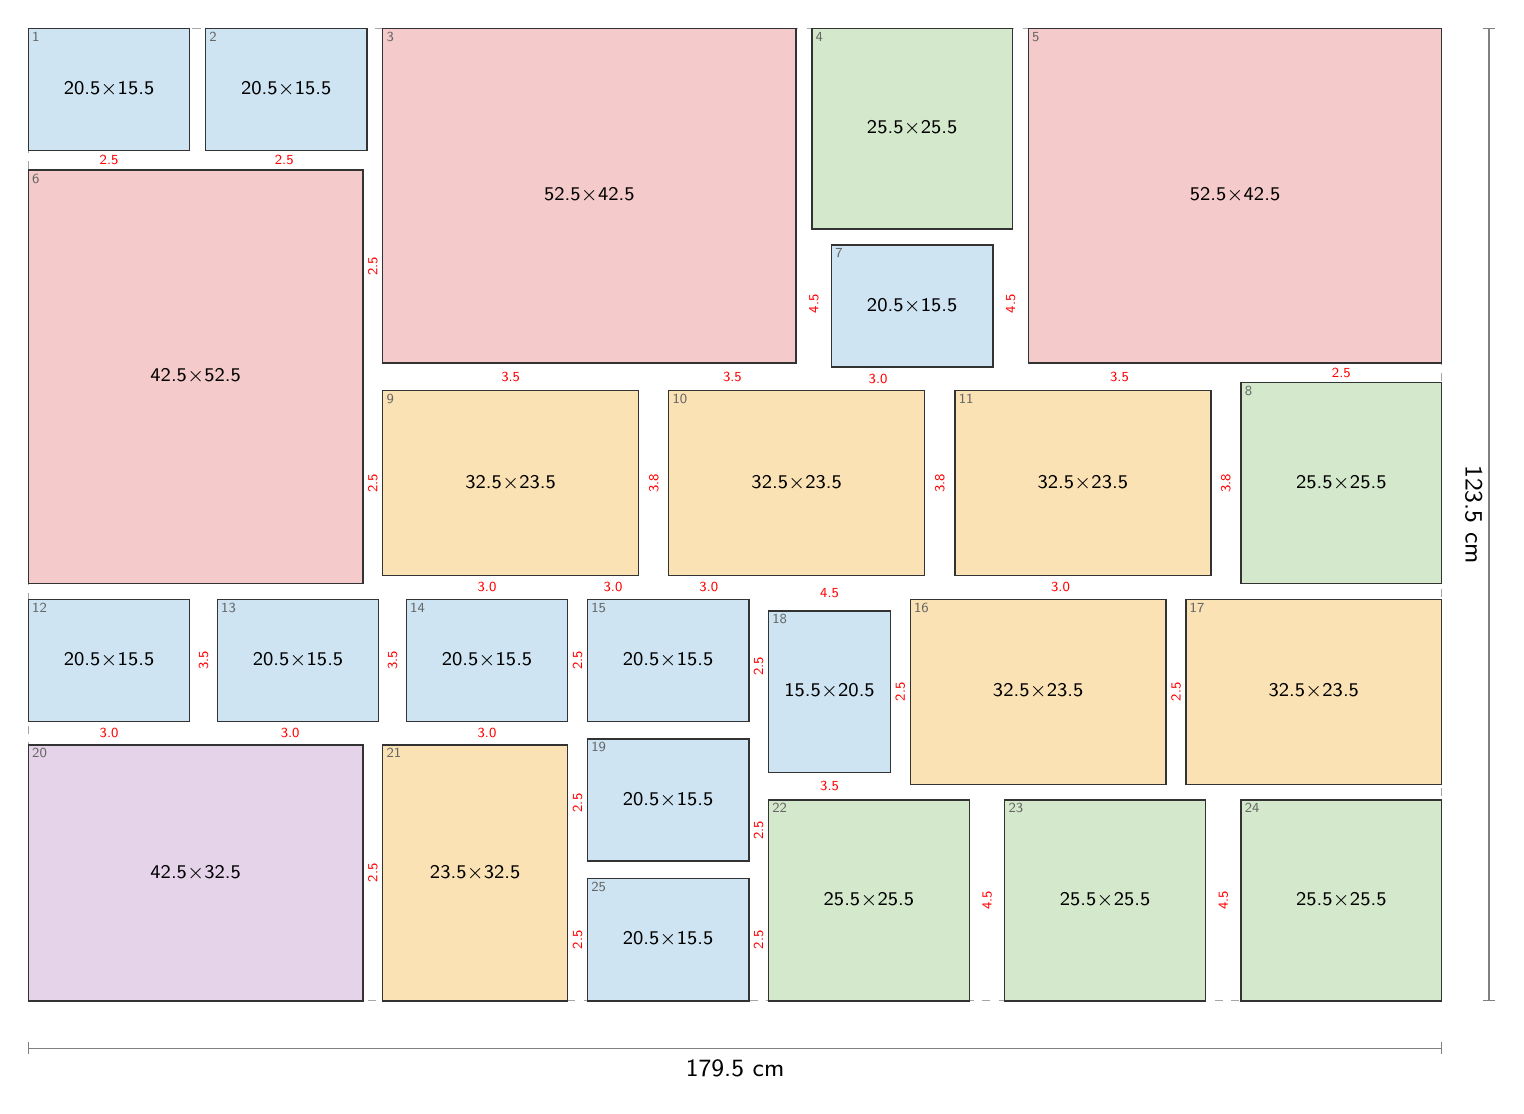
\begin{tikzpicture}[x=1mm, y=-1mm]
\draw[gray!70, dashed, line width=0.4pt] (0,0) rectangle (179.50,123.50);
\filldraw[fill=ft0, draw=black!80, line width=0.5pt] (0.00,0.00) rectangle (20.50,15.50);
\node[align=center, inner sep=0pt] at (10.25,7.75) {\scriptsize 20.5$\times$15.5};
\node[anchor=north west, inner sep=1.2pt, font=\tiny, text=black!60] at (0.00,0.00) {1};
\filldraw[fill=ft0, draw=black!80, line width=0.5pt] (22.50,0.00) rectangle (43.00,15.50);
\node[align=center, inner sep=0pt] at (32.75,7.75) {\scriptsize 20.5$\times$15.5};
\node[anchor=north west, inner sep=1.2pt, font=\tiny, text=black!60] at (22.50,0.00) {2};
\filldraw[fill=ft4, draw=black!80, line width=0.5pt] (45.00,0.00) rectangle (97.50,42.50);
\node[align=center, inner sep=0pt] at (71.25,21.25) {\scriptsize 52.5$\times$42.5};
\node[anchor=north west, inner sep=1.2pt, font=\tiny, text=black!60] at (45.00,0.00) {3};
\filldraw[fill=ft2, draw=black!80, line width=0.5pt] (99.50,0.00) rectangle (125.00,25.50);
\node[align=center, inner sep=0pt] at (112.25,12.75) {\scriptsize 25.5$\times$25.5};
\node[anchor=north west, inner sep=1.2pt, font=\tiny, text=black!60] at (99.50,0.00) {4};
\filldraw[fill=ft4, draw=black!80, line width=0.5pt] (127.00,0.00) rectangle (179.50,42.50);
\node[align=center, inner sep=0pt] at (153.25,21.25) {\scriptsize 52.5$\times$42.5};
\node[anchor=north west, inner sep=1.2pt, font=\tiny, text=black!60] at (127.00,0.00) {5};
\filldraw[fill=ft4, draw=black!80, line width=0.5pt] (0.00,18.00) rectangle (42.50,70.50);
\node[align=center, inner sep=0pt] at (21.25,44.25) {\scriptsize 42.5$\times$52.5};
\node[anchor=north west, inner sep=1.2pt, font=\tiny, text=black!60] at (0.00,18.00) {6};
\filldraw[fill=ft0, draw=black!80, line width=0.5pt] (102.00,27.50) rectangle (122.50,43.00);
\node[align=center, inner sep=0pt] at (112.25,35.25) {\scriptsize 20.5$\times$15.5};
\node[anchor=north west, inner sep=1.2pt, font=\tiny, text=black!60] at (102.00,27.50) {7};
\filldraw[fill=ft2, draw=black!80, line width=0.5pt] (154.00,45.00) rectangle (179.50,70.50);
\node[align=center, inner sep=0pt] at (166.75,57.75) {\scriptsize 25.5$\times$25.5};
\node[anchor=north west, inner sep=1.2pt, font=\tiny, text=black!60] at (154.00,45.00) {8};
\filldraw[fill=ft1, draw=black!80, line width=0.5pt] (45.00,46.00) rectangle (77.50,69.50);
\node[align=center, inner sep=0pt] at (61.25,57.75) {\scriptsize 32.5$\times$23.5};
\node[anchor=north west, inner sep=1.2pt, font=\tiny, text=black!60] at (45.00,46.00) {9};
\filldraw[fill=ft1, draw=black!80, line width=0.5pt] (81.33,46.00) rectangle (113.83,69.50);
\node[align=center, inner sep=0pt] at (97.58,57.75) {\scriptsize 32.5$\times$23.5};
\node[anchor=north west, inner sep=1.2pt, font=\tiny, text=black!60] at (81.33,46.00) {10};
\filldraw[fill=ft1, draw=black!80, line width=0.5pt] (117.67,46.00) rectangle (150.17,69.50);
\node[align=center, inner sep=0pt] at (133.92,57.75) {\scriptsize 32.5$\times$23.5};
\node[anchor=north west, inner sep=1.2pt, font=\tiny, text=black!60] at (117.67,46.00) {11};
\filldraw[fill=ft0, draw=black!80, line width=0.5pt] (0.00,72.50) rectangle (20.50,88.00);
\node[align=center, inner sep=0pt] at (10.25,80.25) {\scriptsize 20.5$\times$15.5};
\node[anchor=north west, inner sep=1.2pt, font=\tiny, text=black!60] at (0.00,72.50) {12};
\filldraw[fill=ft0, draw=black!80, line width=0.5pt] (24.00,72.50) rectangle (44.50,88.00);
\node[align=center, inner sep=0pt] at (34.25,80.25) {\scriptsize 20.5$\times$15.5};
\node[anchor=north west, inner sep=1.2pt, font=\tiny, text=black!60] at (24.00,72.50) {13};
\filldraw[fill=ft0, draw=black!80, line width=0.5pt] (48.00,72.50) rectangle (68.50,88.00);
\node[align=center, inner sep=0pt] at (58.25,80.25) {\scriptsize 20.5$\times$15.5};
\node[anchor=north west, inner sep=1.2pt, font=\tiny, text=black!60] at (48.00,72.50) {14};
\filldraw[fill=ft0, draw=black!80, line width=0.5pt] (71.00,72.50) rectangle (91.50,88.00);
\node[align=center, inner sep=0pt] at (81.25,80.25) {\scriptsize 20.5$\times$15.5};
\node[anchor=north west, inner sep=1.2pt, font=\tiny, text=black!60] at (71.00,72.50) {15};
\filldraw[fill=ft1, draw=black!80, line width=0.5pt] (112.00,72.50) rectangle (144.50,96.00);
\node[align=center, inner sep=0pt] at (128.25,84.25) {\scriptsize 32.5$\times$23.5};
\node[anchor=north west, inner sep=1.2pt, font=\tiny, text=black!60] at (112.00,72.50) {16};
\filldraw[fill=ft1, draw=black!80, line width=0.5pt] (147.00,72.50) rectangle (179.50,96.00);
\node[align=center, inner sep=0pt] at (163.25,84.25) {\scriptsize 32.5$\times$23.5};
\node[anchor=north west, inner sep=1.2pt, font=\tiny, text=black!60] at (147.00,72.50) {17};
\filldraw[fill=ft0, draw=black!80, line width=0.5pt] (94.00,74.00) rectangle (109.50,94.50);
\node[align=center, inner sep=0pt] at (101.75,84.25) {\scriptsize 15.5$\times$20.5};
\node[anchor=north west, inner sep=1.2pt, font=\tiny, text=black!60] at (94.00,74.00) {18};
\filldraw[fill=ft0, draw=black!80, line width=0.5pt] (71.00,90.25) rectangle (91.50,105.75);
\node[align=center, inner sep=0pt] at (81.25,98.00) {\scriptsize 20.5$\times$15.5};
\node[anchor=north west, inner sep=1.2pt, font=\tiny, text=black!60] at (71.00,90.25) {19};
\filldraw[fill=ft3, draw=black!80, line width=0.5pt] (0.00,91.00) rectangle (42.50,123.50);
\node[align=center, inner sep=0pt] at (21.25,107.25) {\scriptsize 42.5$\times$32.5};
\node[anchor=north west, inner sep=1.2pt, font=\tiny, text=black!60] at (0.00,91.00) {20};
\filldraw[fill=ft1, draw=black!80, line width=0.5pt] (45.00,91.00) rectangle (68.50,123.50);
\node[align=center, inner sep=0pt] at (56.75,107.25) {\scriptsize 23.5$\times$32.5};
\node[anchor=north west, inner sep=1.2pt, font=\tiny, text=black!60] at (45.00,91.00) {21};
\filldraw[fill=ft2, draw=black!80, line width=0.5pt] (94.00,98.00) rectangle (119.50,123.50);
\node[align=center, inner sep=0pt] at (106.75,110.75) {\scriptsize 25.5$\times$25.5};
\node[anchor=north west, inner sep=1.2pt, font=\tiny, text=black!60] at (94.00,98.00) {22};
\filldraw[fill=ft2, draw=black!80, line width=0.5pt] (124.00,98.00) rectangle (149.50,123.50);
\node[align=center, inner sep=0pt] at (136.75,110.75) {\scriptsize 25.5$\times$25.5};
\node[anchor=north west, inner sep=1.2pt, font=\tiny, text=black!60] at (124.00,98.00) {23};
\filldraw[fill=ft2, draw=black!80, line width=0.5pt] (154.00,98.00) rectangle (179.50,123.50);
\node[align=center, inner sep=0pt] at (166.75,110.75) {\scriptsize 25.5$\times$25.5};
\node[anchor=north west, inner sep=1.2pt, font=\tiny, text=black!60] at (154.00,98.00) {24};
\filldraw[fill=ft0, draw=black!80, line width=0.5pt] (71.00,108.00) rectangle (91.50,123.50);
\node[align=center, inner sep=0pt] at (81.25,115.75) {\scriptsize 20.5$\times$15.5};
\node[anchor=north west, inner sep=1.2pt, font=\tiny, text=black!60] at (71.00,108.00) {25};
\node[font=\tiny, text=red, fill=white, inner sep=0.3pt] at (10.25,16.75) {2.5};
\node[font=\tiny, text=red, fill=white, inner sep=0.3pt] at (32.50,16.75) {2.5};
\node[font=\tiny, text=red, fill=white, inner sep=0.3pt, rotate=90] at (99.75,35.00) {4.5};
\node[font=\tiny, text=red, fill=white, inner sep=0.3pt] at (61.25,44.25) {3.5};
\node[font=\tiny, text=red, fill=white, inner sep=0.3pt] at (89.42,44.25) {3.5};
\node[font=\tiny, text=red, fill=white, inner sep=0.3pt] at (166.75,43.75) {2.5};
\node[font=\tiny, text=red, fill=white, inner sep=0.3pt] at (138.58,44.25) {3.5};
\node[font=\tiny, text=red, fill=white, inner sep=0.3pt, rotate=90] at (43.75,30.25) {2.5};
\node[font=\tiny, text=red, fill=white, inner sep=0.3pt, rotate=90] at (43.75,57.75) {2.5};
\node[font=\tiny, text=red, fill=white, inner sep=0.3pt, rotate=90] at (124.75,35.00) {4.5};
\node[font=\tiny, text=red, fill=white, inner sep=0.3pt] at (107.92,44.50) {3.0};
\node[font=\tiny, text=red, fill=white, inner sep=0.3pt, rotate=90] at (79.42,57.75) {3.8};
\node[font=\tiny, text=red, fill=white, inner sep=0.3pt] at (58.25,71.00) {3.0};
\node[font=\tiny, text=red, fill=white, inner sep=0.3pt] at (74.25,71.00) {3.0};
\node[font=\tiny, text=red, fill=white, inner sep=0.3pt, rotate=90] at (115.75,57.75) {3.8};
\node[font=\tiny, text=red, fill=white, inner sep=0.3pt] at (86.42,71.00) {3.0};
\node[font=\tiny, text=red, fill=white, inner sep=0.3pt] at (101.75,71.75) {4.5};
\node[font=\tiny, text=red, fill=white, inner sep=0.3pt, rotate=90] at (152.08,57.75) {3.8};
\node[font=\tiny, text=red, fill=white, inner sep=0.3pt] at (131.08,71.00) {3.0};
\node[font=\tiny, text=red, fill=white, inner sep=0.3pt, rotate=90] at (22.25,80.25) {3.5};
\node[font=\tiny, text=red, fill=white, inner sep=0.3pt] at (10.25,89.50) {3.0};
\node[font=\tiny, text=red, fill=white, inner sep=0.3pt, rotate=90] at (46.25,80.25) {3.5};
\node[font=\tiny, text=red, fill=white, inner sep=0.3pt] at (33.25,89.50) {3.0};
\node[font=\tiny, text=red, fill=white, inner sep=0.3pt, rotate=90] at (69.75,80.25) {2.5};
\node[font=\tiny, text=red, fill=white, inner sep=0.3pt] at (58.25,89.50) {3.0};
\node[font=\tiny, text=red, fill=white, inner sep=0.3pt, rotate=90] at (92.75,81.00) {2.5};
\node[font=\tiny, text=red, fill=white, inner sep=0.3pt, rotate=90] at (145.75,84.25) {2.5};
\node[font=\tiny, text=red, fill=white, inner sep=0.3pt, rotate=90] at (110.75,84.25) {2.5};
\node[font=\tiny, text=red, fill=white, inner sep=0.3pt] at (101.75,96.25) {3.5};
\node[font=\tiny, text=red, fill=white, inner sep=0.3pt, rotate=90] at (92.75,101.88) {2.5};
\node[font=\tiny, text=red, fill=white, inner sep=0.3pt, rotate=90] at (43.75,107.25) {2.5};
\node[font=\tiny, text=red, fill=white, inner sep=0.3pt, rotate=90] at (69.75,98.38) {2.5};
\node[font=\tiny, text=red, fill=white, inner sep=0.3pt, rotate=90] at (69.75,115.75) {2.5};
\node[font=\tiny, text=red, fill=white, inner sep=0.3pt, rotate=90] at (121.75,110.75) {4.5};
\node[font=\tiny, text=red, fill=white, inner sep=0.3pt, rotate=90] at (151.75,110.75) {4.5};
\node[font=\tiny, text=red, fill=white, inner sep=0.3pt, rotate=90] at (92.75,115.75) {2.5};
\draw[Bar-Bar, gray] (0,129.50) -- (179.50,129.50) node[midway, below=1pt, font=\small, text=black] {179.5 cm};
\draw[Bar-Bar, gray] (185.50,0) -- (185.50,123.50) node[midway, right=1pt, font=\small, text=black, rotate=-90, anchor=north] {123.5 cm};
\end{tikzpicture}\\[4pt]
{\scriptsize Scale 1:10 (1 mm = 1 cm). Red numbers mark gaps that deviate from the nominal gap by more than 0.25 cm. Small grey numbers index the coordinate table.}
\end{minipage}\hfill
\begin{minipage}[t]{0.25\textwidth}\vspace{0pt}
\small
\begin{tabular}{@{}l l@{}}
\toprule
Outer size & 179.5 $\times$ 123.5 cm \\
Nominal gap & 2 cm \\
Actual gaps & 2.0 -- 4.5 cm \\
Max.\ deviation & 2.5 cm \\
Mean deviation & 0.87 cm \\
Border notches & bottom 9 cm \\
Corners filled & 4 / 4 \\
Frames used & 25 of 28 \\
Large frames & {\scriptsize 3, touching 1$\times$ (24 cm), min.\ dist.\ 55 cm} \\
Entropy & 0.73 \\
\quad {\scriptsize mix / variety} & {\scriptsize 0.79 / 0.83} \\
\quad {\scriptsize stagger / lines} & {\scriptsize 0.55 / 0.75 (2 through)} \\
\bottomrule
\end{tabular}

\vspace{8pt}
\scriptsize
\begin{tabular}{@{}c l l r r@{}}
\toprule
 & outer w $\times$ h (cm) &  & used & have \\
\midrule
\tikz[baseline=-0.6ex]\fill[ft0,draw=black!60] (0,0) rectangle (1.2ex,1.2ex); & 20.5$\times$15.5 & L & 9 & 9 \\
\tikz[baseline=-0.6ex]\fill[ft0,draw=black!60] (0,0) rectangle (1.2ex,1.2ex); & 15.5$\times$20.5 & P & 1 & 2 \\
\tikz[baseline=-0.6ex]\fill[ft3,draw=black!60] (0,0) rectangle (1.2ex,1.2ex); & 32.5$\times$42.5 & P & 0 & 2 \\
\tikz[baseline=-0.6ex]\fill[ft3,draw=black!60] (0,0) rectangle (1.2ex,1.2ex); & 42.5$\times$32.5 & L & 1 & 1 \\
\tikz[baseline=-0.6ex]\fill[ft1,draw=black!60] (0,0) rectangle (1.2ex,1.2ex); & 32.5$\times$23.5 & L & 5 & 5 \\
\tikz[baseline=-0.6ex]\fill[ft1,draw=black!60] (0,0) rectangle (1.2ex,1.2ex); & 23.5$\times$32.5 & P & 1 & 1 \\
\tikz[baseline=-0.6ex]\fill[ft2,draw=black!60] (0,0) rectangle (1.2ex,1.2ex); & 25.5$\times$25.5 &  & 5 & 5 \\
\tikz[baseline=-0.6ex]\fill[ft4,draw=black!60] (0,0) rectangle (1.2ex,1.2ex); & 42.5$\times$52.5 & P & 1 & 1 \\
\tikz[baseline=-0.6ex]\fill[ft4,draw=black!60] (0,0) rectangle (1.2ex,1.2ex); & 52.5$\times$42.5 & L & 2 & 2 \\
\bottomrule
\end{tabular}

\vspace{8pt}
{\bfseries Positions} (top-left corner, cm)\\[2pt]
\tiny
\begin{tabular}{@{}r l r r@{}}
\toprule
\# & frame w $\times$ h & x & y \\
\midrule
1 & 20.5 $\times$ 15.5 & 0.0 & 0.0 \\
2 & 20.5 $\times$ 15.5 & 22.5 & 0.0 \\
3 & 52.5 $\times$ 42.5 & 45.0 & 0.0 \\
4 & 25.5 $\times$ 25.5 & 99.5 & 0.0 \\
5 & 52.5 $\times$ 42.5 & 127.0 & 0.0 \\
6 & 42.5 $\times$ 52.5 & 0.0 & 18.0 \\
7 & 20.5 $\times$ 15.5 & 102.0 & 27.5 \\
8 & 25.5 $\times$ 25.5 & 154.0 & 45.0 \\
9 & 32.5 $\times$ 23.5 & 45.0 & 46.0 \\
10 & 32.5 $\times$ 23.5 & 81.3 & 46.0 \\
11 & 32.5 $\times$ 23.5 & 117.7 & 46.0 \\
12 & 20.5 $\times$ 15.5 & 0.0 & 72.5 \\
13 & 20.5 $\times$ 15.5 & 24.0 & 72.5 \\
14 & 20.5 $\times$ 15.5 & 48.0 & 72.5 \\
15 & 20.5 $\times$ 15.5 & 71.0 & 72.5 \\
16 & 32.5 $\times$ 23.5 & 112.0 & 72.5 \\
17 & 32.5 $\times$ 23.5 & 147.0 & 72.5 \\
18 & 15.5 $\times$ 20.5 & 94.0 & 74.0 \\
19 & 20.5 $\times$ 15.5 & 71.0 & 90.2 \\
20 & 42.5 $\times$ 32.5 & 0.0 & 91.0 \\
21 & 23.5 $\times$ 32.5 & 45.0 & 91.0 \\
22 & 25.5 $\times$ 25.5 & 94.0 & 98.0 \\
23 & 25.5 $\times$ 25.5 & 124.0 & 98.0 \\
24 & 25.5 $\times$ 25.5 & 154.0 & 98.0 \\
25 & 20.5 $\times$ 15.5 & 71.0 & 108.0 \\
\bottomrule
\end{tabular}
\end{minipage}
\clearpage

\phantomsection\addcontentsline{toc}{subsection}{Layout 6: 177.5 \texorpdfstring{$\times$}{x} 126.5 cm, 24 frames, gap 1.5 cm, max.\ deviation 3.0 cm}
\label{lay:per-run-gap:6}
\begin{minipage}[t]{0.74\textwidth}\vspace{0pt}
{\LARGE\bfseries Layout 6}\hspace{1.5em}{\large 177.5 $\times$ 126.5 cm \quad gap 1.5 cm \quad 24 frames}\\[8pt]
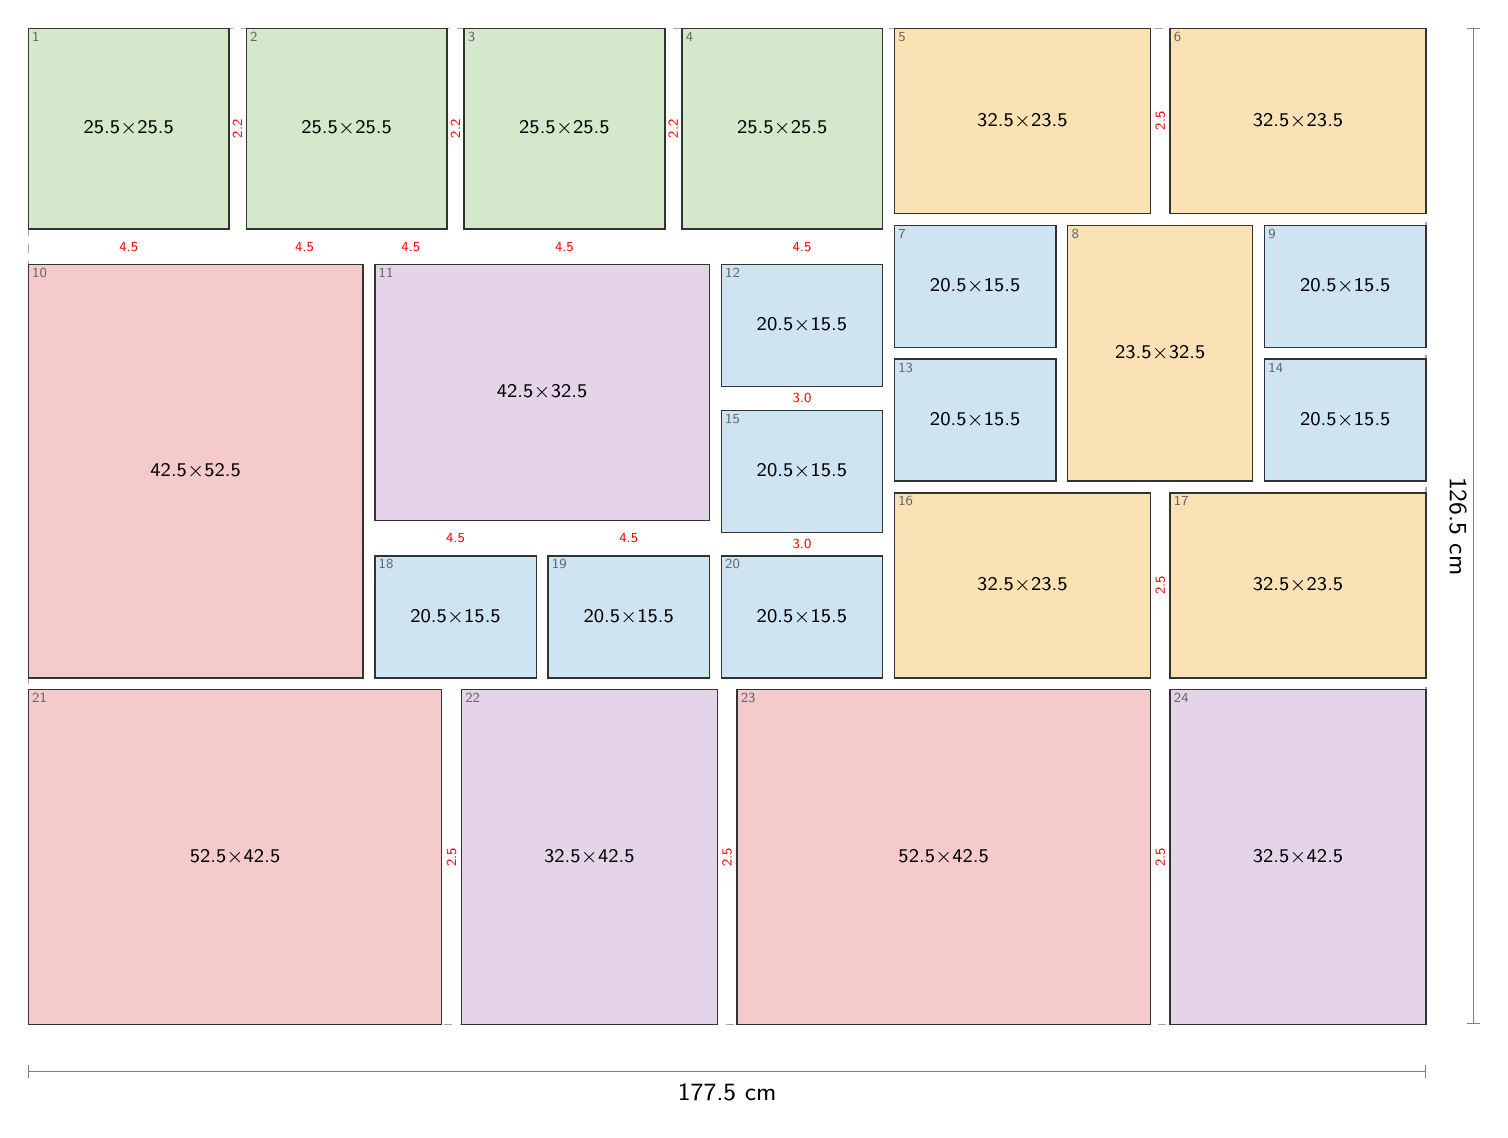
\begin{tikzpicture}[x=1mm, y=-1mm]
\draw[gray!70, dashed, line width=0.4pt] (0,0) rectangle (177.50,126.50);
\filldraw[fill=ft2, draw=black!80, line width=0.5pt] (0.00,0.00) rectangle (25.50,25.50);
\node[align=center, inner sep=0pt] at (12.75,12.75) {\scriptsize 25.5$\times$25.5};
\node[anchor=north west, inner sep=1.2pt, font=\tiny, text=black!60] at (0.00,0.00) {1};
\filldraw[fill=ft2, draw=black!80, line width=0.5pt] (27.67,0.00) rectangle (53.17,25.50);
\node[align=center, inner sep=0pt] at (40.42,12.75) {\scriptsize 25.5$\times$25.5};
\node[anchor=north west, inner sep=1.2pt, font=\tiny, text=black!60] at (27.67,0.00) {2};
\filldraw[fill=ft2, draw=black!80, line width=0.5pt] (55.33,0.00) rectangle (80.83,25.50);
\node[align=center, inner sep=0pt] at (68.08,12.75) {\scriptsize 25.5$\times$25.5};
\node[anchor=north west, inner sep=1.2pt, font=\tiny, text=black!60] at (55.33,0.00) {3};
\filldraw[fill=ft2, draw=black!80, line width=0.5pt] (83.00,0.00) rectangle (108.50,25.50);
\node[align=center, inner sep=0pt] at (95.75,12.75) {\scriptsize 25.5$\times$25.5};
\node[anchor=north west, inner sep=1.2pt, font=\tiny, text=black!60] at (83.00,0.00) {4};
\filldraw[fill=ft1, draw=black!80, line width=0.5pt] (110.00,0.00) rectangle (142.50,23.50);
\node[align=center, inner sep=0pt] at (126.25,11.75) {\scriptsize 32.5$\times$23.5};
\node[anchor=north west, inner sep=1.2pt, font=\tiny, text=black!60] at (110.00,0.00) {5};
\filldraw[fill=ft1, draw=black!80, line width=0.5pt] (145.00,0.00) rectangle (177.50,23.50);
\node[align=center, inner sep=0pt] at (161.25,11.75) {\scriptsize 32.5$\times$23.5};
\node[anchor=north west, inner sep=1.2pt, font=\tiny, text=black!60] at (145.00,0.00) {6};
\filldraw[fill=ft0, draw=black!80, line width=0.5pt] (110.00,25.00) rectangle (130.50,40.50);
\node[align=center, inner sep=0pt] at (120.25,32.75) {\scriptsize 20.5$\times$15.5};
\node[anchor=north west, inner sep=1.2pt, font=\tiny, text=black!60] at (110.00,25.00) {7};
\filldraw[fill=ft1, draw=black!80, line width=0.5pt] (132.00,25.00) rectangle (155.50,57.50);
\node[align=center, inner sep=0pt] at (143.75,41.25) {\scriptsize 23.5$\times$32.5};
\node[anchor=north west, inner sep=1.2pt, font=\tiny, text=black!60] at (132.00,25.00) {8};
\filldraw[fill=ft0, draw=black!80, line width=0.5pt] (157.00,25.00) rectangle (177.50,40.50);
\node[align=center, inner sep=0pt] at (167.25,32.75) {\scriptsize 20.5$\times$15.5};
\node[anchor=north west, inner sep=1.2pt, font=\tiny, text=black!60] at (157.00,25.00) {9};
\filldraw[fill=ft4, draw=black!80, line width=0.5pt] (0.00,30.00) rectangle (42.50,82.50);
\node[align=center, inner sep=0pt] at (21.25,56.25) {\scriptsize 42.5$\times$52.5};
\node[anchor=north west, inner sep=1.2pt, font=\tiny, text=black!60] at (0.00,30.00) {10};
\filldraw[fill=ft3, draw=black!80, line width=0.5pt] (44.00,30.00) rectangle (86.50,62.50);
\node[align=center, inner sep=0pt] at (65.25,46.25) {\scriptsize 42.5$\times$32.5};
\node[anchor=north west, inner sep=1.2pt, font=\tiny, text=black!60] at (44.00,30.00) {11};
\filldraw[fill=ft0, draw=black!80, line width=0.5pt] (88.00,30.00) rectangle (108.50,45.50);
\node[align=center, inner sep=0pt] at (98.25,37.75) {\scriptsize 20.5$\times$15.5};
\node[anchor=north west, inner sep=1.2pt, font=\tiny, text=black!60] at (88.00,30.00) {12};
\filldraw[fill=ft0, draw=black!80, line width=0.5pt] (110.00,42.00) rectangle (130.50,57.50);
\node[align=center, inner sep=0pt] at (120.25,49.75) {\scriptsize 20.5$\times$15.5};
\node[anchor=north west, inner sep=1.2pt, font=\tiny, text=black!60] at (110.00,42.00) {13};
\filldraw[fill=ft0, draw=black!80, line width=0.5pt] (157.00,42.00) rectangle (177.50,57.50);
\node[align=center, inner sep=0pt] at (167.25,49.75) {\scriptsize 20.5$\times$15.5};
\node[anchor=north west, inner sep=1.2pt, font=\tiny, text=black!60] at (157.00,42.00) {14};
\filldraw[fill=ft0, draw=black!80, line width=0.5pt] (88.00,48.50) rectangle (108.50,64.00);
\node[align=center, inner sep=0pt] at (98.25,56.25) {\scriptsize 20.5$\times$15.5};
\node[anchor=north west, inner sep=1.2pt, font=\tiny, text=black!60] at (88.00,48.50) {15};
\filldraw[fill=ft1, draw=black!80, line width=0.5pt] (110.00,59.00) rectangle (142.50,82.50);
\node[align=center, inner sep=0pt] at (126.25,70.75) {\scriptsize 32.5$\times$23.5};
\node[anchor=north west, inner sep=1.2pt, font=\tiny, text=black!60] at (110.00,59.00) {16};
\filldraw[fill=ft1, draw=black!80, line width=0.5pt] (145.00,59.00) rectangle (177.50,82.50);
\node[align=center, inner sep=0pt] at (161.25,70.75) {\scriptsize 32.5$\times$23.5};
\node[anchor=north west, inner sep=1.2pt, font=\tiny, text=black!60] at (145.00,59.00) {17};
\filldraw[fill=ft0, draw=black!80, line width=0.5pt] (44.00,67.00) rectangle (64.50,82.50);
\node[align=center, inner sep=0pt] at (54.25,74.75) {\scriptsize 20.5$\times$15.5};
\node[anchor=north west, inner sep=1.2pt, font=\tiny, text=black!60] at (44.00,67.00) {18};
\filldraw[fill=ft0, draw=black!80, line width=0.5pt] (66.00,67.00) rectangle (86.50,82.50);
\node[align=center, inner sep=0pt] at (76.25,74.75) {\scriptsize 20.5$\times$15.5};
\node[anchor=north west, inner sep=1.2pt, font=\tiny, text=black!60] at (66.00,67.00) {19};
\filldraw[fill=ft0, draw=black!80, line width=0.5pt] (88.00,67.00) rectangle (108.50,82.50);
\node[align=center, inner sep=0pt] at (98.25,74.75) {\scriptsize 20.5$\times$15.5};
\node[anchor=north west, inner sep=1.2pt, font=\tiny, text=black!60] at (88.00,67.00) {20};
\filldraw[fill=ft4, draw=black!80, line width=0.5pt] (0.00,84.00) rectangle (52.50,126.50);
\node[align=center, inner sep=0pt] at (26.25,105.25) {\scriptsize 52.5$\times$42.5};
\node[anchor=north west, inner sep=1.2pt, font=\tiny, text=black!60] at (0.00,84.00) {21};
\filldraw[fill=ft3, draw=black!80, line width=0.5pt] (55.00,84.00) rectangle (87.50,126.50);
\node[align=center, inner sep=0pt] at (71.25,105.25) {\scriptsize 32.5$\times$42.5};
\node[anchor=north west, inner sep=1.2pt, font=\tiny, text=black!60] at (55.00,84.00) {22};
\filldraw[fill=ft4, draw=black!80, line width=0.5pt] (90.00,84.00) rectangle (142.50,126.50);
\node[align=center, inner sep=0pt] at (116.25,105.25) {\scriptsize 52.5$\times$42.5};
\node[anchor=north west, inner sep=1.2pt, font=\tiny, text=black!60] at (90.00,84.00) {23};
\filldraw[fill=ft3, draw=black!80, line width=0.5pt] (145.00,84.00) rectangle (177.50,126.50);
\node[align=center, inner sep=0pt] at (161.25,105.25) {\scriptsize 32.5$\times$42.5};
\node[anchor=north west, inner sep=1.2pt, font=\tiny, text=black!60] at (145.00,84.00) {24};
\node[font=\tiny, text=red, fill=white, inner sep=0.3pt, rotate=90] at (26.58,12.75) {2.2};
\node[font=\tiny, text=red, fill=white, inner sep=0.3pt] at (12.75,27.75) {4.5};
\node[font=\tiny, text=red, fill=white, inner sep=0.3pt, rotate=90] at (54.25,12.75) {2.2};
\node[font=\tiny, text=red, fill=white, inner sep=0.3pt] at (35.08,27.75) {4.5};
\node[font=\tiny, text=red, fill=white, inner sep=0.3pt] at (48.58,27.75) {4.5};
\node[font=\tiny, text=red, fill=white, inner sep=0.3pt, rotate=90] at (81.92,12.75) {2.2};
\node[font=\tiny, text=red, fill=white, inner sep=0.3pt] at (68.08,27.75) {4.5};
\node[font=\tiny, text=red, fill=white, inner sep=0.3pt] at (98.25,27.75) {4.5};
\node[font=\tiny, text=red, fill=white, inner sep=0.3pt, rotate=90] at (143.75,11.75) {2.5};
\node[font=\tiny, text=red, fill=white, inner sep=0.3pt] at (54.25,64.75) {4.5};
\node[font=\tiny, text=red, fill=white, inner sep=0.3pt] at (76.25,64.75) {4.5};
\node[font=\tiny, text=red, fill=white, inner sep=0.3pt] at (98.25,47.00) {3.0};
\node[font=\tiny, text=red, fill=white, inner sep=0.3pt] at (98.25,65.50) {3.0};
\node[font=\tiny, text=red, fill=white, inner sep=0.3pt, rotate=90] at (143.75,70.75) {2.5};
\node[font=\tiny, text=red, fill=white, inner sep=0.3pt, rotate=90] at (53.75,105.25) {2.5};
\node[font=\tiny, text=red, fill=white, inner sep=0.3pt, rotate=90] at (88.75,105.25) {2.5};
\node[font=\tiny, text=red, fill=white, inner sep=0.3pt, rotate=90] at (143.75,105.25) {2.5};
\draw[Bar-Bar, gray] (0,132.50) -- (177.50,132.50) node[midway, below=1pt, font=\small, text=black] {177.5 cm};
\draw[Bar-Bar, gray] (183.50,0) -- (183.50,126.50) node[midway, right=1pt, font=\small, text=black, rotate=-90, anchor=north] {126.5 cm};
\end{tikzpicture}\\[4pt]
{\scriptsize Scale 1:10 (1 mm = 1 cm). Red numbers mark gaps that deviate from the nominal gap by more than 0.25 cm. Small grey numbers index the coordinate table.}
\end{minipage}\hfill
\begin{minipage}[t]{0.25\textwidth}\vspace{0pt}
\small
\begin{tabular}{@{}l l@{}}
\toprule
Outer size & 177.5 $\times$ 126.5 cm \\
Nominal gap & 1.5 cm \\
Actual gaps & 1.5 -- 4.5 cm \\
Max.\ deviation & 3.0 cm \\
Mean deviation & 0.63 cm \\
Border notches & left 4 cm \\
Corners filled & 4 / 4 \\
Frames used & 24 of 28 \\
Large frames & {\scriptsize 3, touching 1$\times$ (42 cm), min.\ dist.\ 49 cm} \\
Entropy & 0.75 \\
\quad {\scriptsize mix / variety} & {\scriptsize 0.81 / 0.72} \\
\quad {\scriptsize stagger / lines} & {\scriptsize 0.45 / 1.00 (1 through)} \\
\bottomrule
\end{tabular}

\vspace{8pt}
\scriptsize
\begin{tabular}{@{}c l l r r@{}}
\toprule
 & outer w $\times$ h (cm) &  & used & have \\
\midrule
\tikz[baseline=-0.6ex]\fill[ft0,draw=black!60] (0,0) rectangle (1.2ex,1.2ex); & 20.5$\times$15.5 & L & 9 & 9 \\
\tikz[baseline=-0.6ex]\fill[ft0,draw=black!60] (0,0) rectangle (1.2ex,1.2ex); & 15.5$\times$20.5 & P & 0 & 2 \\
\tikz[baseline=-0.6ex]\fill[ft3,draw=black!60] (0,0) rectangle (1.2ex,1.2ex); & 32.5$\times$42.5 & P & 2 & 2 \\
\tikz[baseline=-0.6ex]\fill[ft3,draw=black!60] (0,0) rectangle (1.2ex,1.2ex); & 42.5$\times$32.5 & L & 1 & 1 \\
\tikz[baseline=-0.6ex]\fill[ft1,draw=black!60] (0,0) rectangle (1.2ex,1.2ex); & 32.5$\times$23.5 & L & 4 & 5 \\
\tikz[baseline=-0.6ex]\fill[ft1,draw=black!60] (0,0) rectangle (1.2ex,1.2ex); & 23.5$\times$32.5 & P & 1 & 1 \\
\tikz[baseline=-0.6ex]\fill[ft2,draw=black!60] (0,0) rectangle (1.2ex,1.2ex); & 25.5$\times$25.5 &  & 4 & 5 \\
\tikz[baseline=-0.6ex]\fill[ft4,draw=black!60] (0,0) rectangle (1.2ex,1.2ex); & 42.5$\times$52.5 & P & 1 & 1 \\
\tikz[baseline=-0.6ex]\fill[ft4,draw=black!60] (0,0) rectangle (1.2ex,1.2ex); & 52.5$\times$42.5 & L & 2 & 2 \\
\bottomrule
\end{tabular}

\vspace{8pt}
{\bfseries Positions} (top-left corner, cm)\\[2pt]
\tiny
\begin{tabular}{@{}r l r r@{}}
\toprule
\# & frame w $\times$ h & x & y \\
\midrule
1 & 25.5 $\times$ 25.5 & 0.0 & 0.0 \\
2 & 25.5 $\times$ 25.5 & 27.7 & 0.0 \\
3 & 25.5 $\times$ 25.5 & 55.3 & 0.0 \\
4 & 25.5 $\times$ 25.5 & 83.0 & 0.0 \\
5 & 32.5 $\times$ 23.5 & 110.0 & 0.0 \\
6 & 32.5 $\times$ 23.5 & 145.0 & 0.0 \\
7 & 20.5 $\times$ 15.5 & 110.0 & 25.0 \\
8 & 23.5 $\times$ 32.5 & 132.0 & 25.0 \\
9 & 20.5 $\times$ 15.5 & 157.0 & 25.0 \\
10 & 42.5 $\times$ 52.5 & 0.0 & 30.0 \\
11 & 42.5 $\times$ 32.5 & 44.0 & 30.0 \\
12 & 20.5 $\times$ 15.5 & 88.0 & 30.0 \\
13 & 20.5 $\times$ 15.5 & 110.0 & 42.0 \\
14 & 20.5 $\times$ 15.5 & 157.0 & 42.0 \\
15 & 20.5 $\times$ 15.5 & 88.0 & 48.5 \\
16 & 32.5 $\times$ 23.5 & 110.0 & 59.0 \\
17 & 32.5 $\times$ 23.5 & 145.0 & 59.0 \\
18 & 20.5 $\times$ 15.5 & 44.0 & 67.0 \\
19 & 20.5 $\times$ 15.5 & 66.0 & 67.0 \\
20 & 20.5 $\times$ 15.5 & 88.0 & 67.0 \\
21 & 52.5 $\times$ 42.5 & 0.0 & 84.0 \\
22 & 32.5 $\times$ 42.5 & 55.0 & 84.0 \\
23 & 52.5 $\times$ 42.5 & 90.0 & 84.0 \\
24 & 32.5 $\times$ 42.5 & 145.0 & 84.0 \\
\bottomrule
\end{tabular}
\end{minipage}
\clearpage

\phantomsection\addcontentsline{toc}{subsection}{Layout 7: 175.5 \texorpdfstring{$\times$}{x} 123.5 cm, 24 frames, gap 2.5 cm, max.\ deviation 4.0 cm}
\label{lay:per-run-gap:7}
\begin{minipage}[t]{0.74\textwidth}\vspace{0pt}
{\LARGE\bfseries Layout 7}\hspace{1.5em}{\large 175.5 $\times$ 123.5 cm \quad gap 2.5 cm \quad 24 frames}\\[8pt]
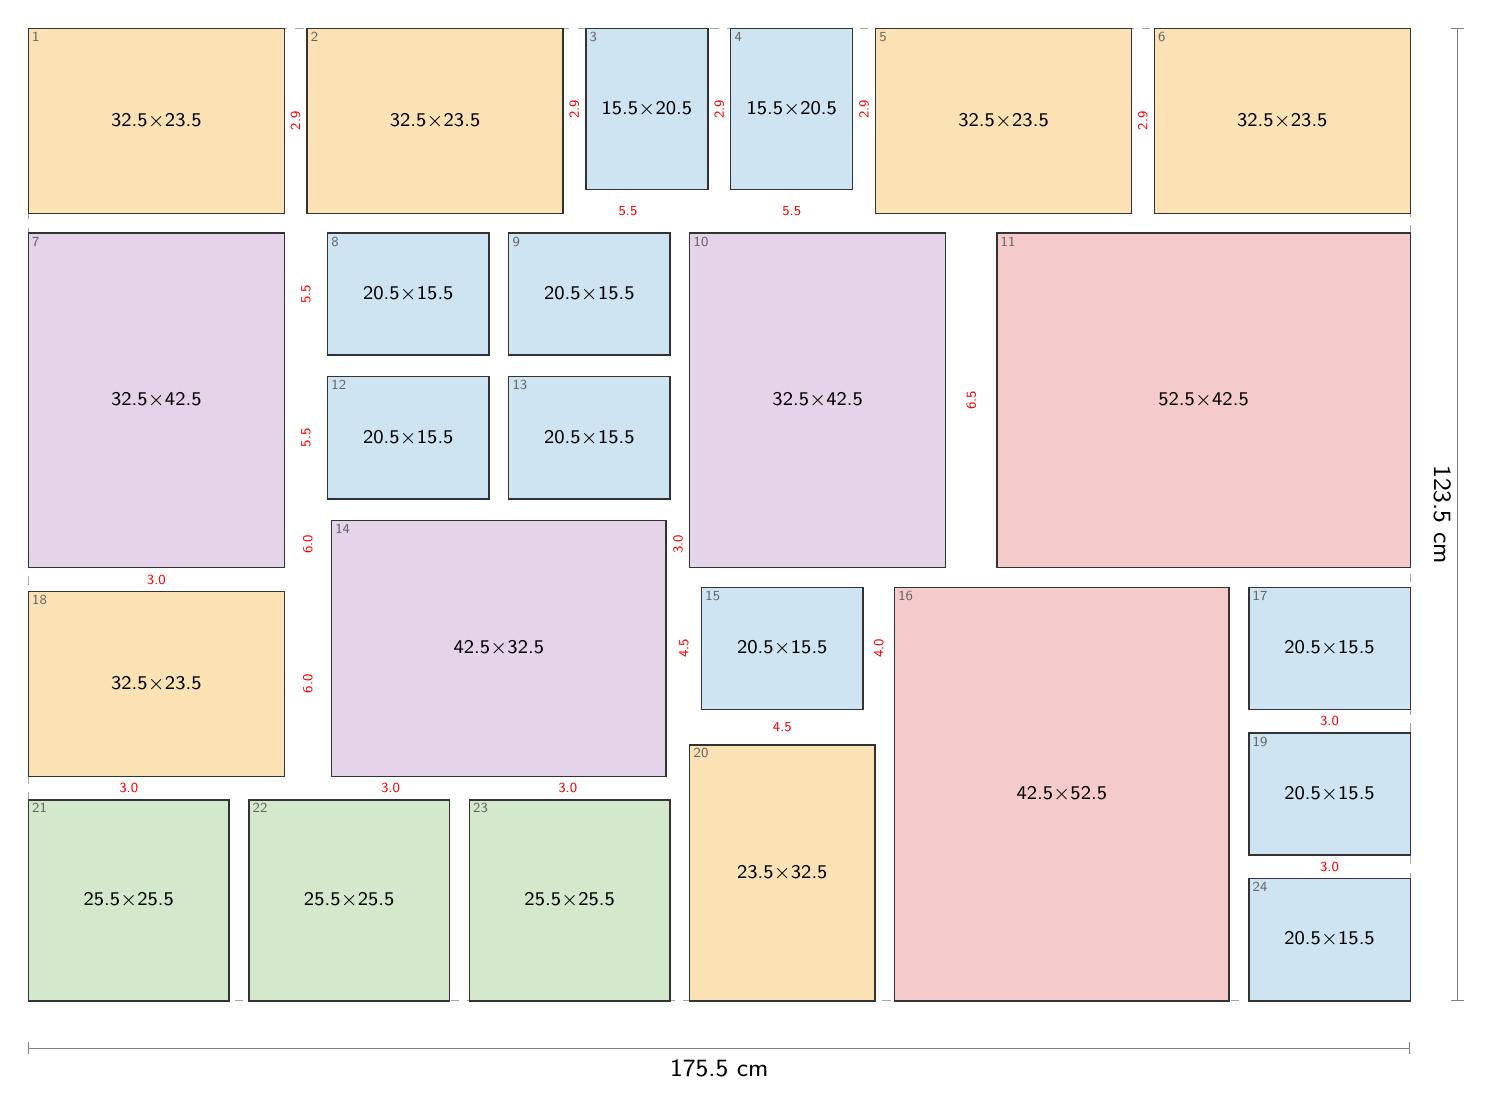
\begin{tikzpicture}[x=1mm, y=-1mm]
\draw[gray!70, dashed, line width=0.4pt] (0,0) rectangle (175.50,123.50);
\filldraw[fill=ft1, draw=black!80, line width=0.5pt] (0.00,0.00) rectangle (32.50,23.50);
\node[align=center, inner sep=0pt] at (16.25,11.75) {\scriptsize 32.5$\times$23.5};
\node[anchor=north west, inner sep=1.2pt, font=\tiny, text=black!60] at (0.00,0.00) {1};
\filldraw[fill=ft1, draw=black!80, line width=0.5pt] (35.40,0.00) rectangle (67.90,23.50);
\node[align=center, inner sep=0pt] at (51.65,11.75) {\scriptsize 32.5$\times$23.5};
\node[anchor=north west, inner sep=1.2pt, font=\tiny, text=black!60] at (35.40,0.00) {2};
\filldraw[fill=ft0, draw=black!80, line width=0.5pt] (70.80,0.00) rectangle (86.30,20.50);
\node[align=center, inner sep=0pt] at (78.55,10.25) {\scriptsize 15.5$\times$20.5};
\node[anchor=north west, inner sep=1.2pt, font=\tiny, text=black!60] at (70.80,0.00) {3};
\filldraw[fill=ft0, draw=black!80, line width=0.5pt] (89.20,0.00) rectangle (104.70,20.50);
\node[align=center, inner sep=0pt] at (96.95,10.25) {\scriptsize 15.5$\times$20.5};
\node[anchor=north west, inner sep=1.2pt, font=\tiny, text=black!60] at (89.20,0.00) {4};
\filldraw[fill=ft1, draw=black!80, line width=0.5pt] (107.60,0.00) rectangle (140.10,23.50);
\node[align=center, inner sep=0pt] at (123.85,11.75) {\scriptsize 32.5$\times$23.5};
\node[anchor=north west, inner sep=1.2pt, font=\tiny, text=black!60] at (107.60,0.00) {5};
\filldraw[fill=ft1, draw=black!80, line width=0.5pt] (143.00,0.00) rectangle (175.50,23.50);
\node[align=center, inner sep=0pt] at (159.25,11.75) {\scriptsize 32.5$\times$23.5};
\node[anchor=north west, inner sep=1.2pt, font=\tiny, text=black!60] at (143.00,0.00) {6};
\filldraw[fill=ft3, draw=black!80, line width=0.5pt] (0.00,26.00) rectangle (32.50,68.50);
\node[align=center, inner sep=0pt] at (16.25,47.25) {\scriptsize 32.5$\times$42.5};
\node[anchor=north west, inner sep=1.2pt, font=\tiny, text=black!60] at (0.00,26.00) {7};
\filldraw[fill=ft0, draw=black!80, line width=0.5pt] (38.00,26.00) rectangle (58.50,41.50);
\node[align=center, inner sep=0pt] at (48.25,33.75) {\scriptsize 20.5$\times$15.5};
\node[anchor=north west, inner sep=1.2pt, font=\tiny, text=black!60] at (38.00,26.00) {8};
\filldraw[fill=ft0, draw=black!80, line width=0.5pt] (61.00,26.00) rectangle (81.50,41.50);
\node[align=center, inner sep=0pt] at (71.25,33.75) {\scriptsize 20.5$\times$15.5};
\node[anchor=north west, inner sep=1.2pt, font=\tiny, text=black!60] at (61.00,26.00) {9};
\filldraw[fill=ft3, draw=black!80, line width=0.5pt] (84.00,26.00) rectangle (116.50,68.50);
\node[align=center, inner sep=0pt] at (100.25,47.25) {\scriptsize 32.5$\times$42.5};
\node[anchor=north west, inner sep=1.2pt, font=\tiny, text=black!60] at (84.00,26.00) {10};
\filldraw[fill=ft4, draw=black!80, line width=0.5pt] (123.00,26.00) rectangle (175.50,68.50);
\node[align=center, inner sep=0pt] at (149.25,47.25) {\scriptsize 52.5$\times$42.5};
\node[anchor=north west, inner sep=1.2pt, font=\tiny, text=black!60] at (123.00,26.00) {11};
\filldraw[fill=ft0, draw=black!80, line width=0.5pt] (38.00,44.25) rectangle (58.50,59.75);
\node[align=center, inner sep=0pt] at (48.25,52.00) {\scriptsize 20.5$\times$15.5};
\node[anchor=north west, inner sep=1.2pt, font=\tiny, text=black!60] at (38.00,44.25) {12};
\filldraw[fill=ft0, draw=black!80, line width=0.5pt] (61.00,44.25) rectangle (81.50,59.75);
\node[align=center, inner sep=0pt] at (71.25,52.00) {\scriptsize 20.5$\times$15.5};
\node[anchor=north west, inner sep=1.2pt, font=\tiny, text=black!60] at (61.00,44.25) {13};
\filldraw[fill=ft3, draw=black!80, line width=0.5pt] (38.50,62.50) rectangle (81.00,95.00);
\node[align=center, inner sep=0pt] at (59.75,78.75) {\scriptsize 42.5$\times$32.5};
\node[anchor=north west, inner sep=1.2pt, font=\tiny, text=black!60] at (38.50,62.50) {14};
\filldraw[fill=ft0, draw=black!80, line width=0.5pt] (85.50,71.00) rectangle (106.00,86.50);
\node[align=center, inner sep=0pt] at (95.75,78.75) {\scriptsize 20.5$\times$15.5};
\node[anchor=north west, inner sep=1.2pt, font=\tiny, text=black!60] at (85.50,71.00) {15};
\filldraw[fill=ft4, draw=black!80, line width=0.5pt] (110.00,71.00) rectangle (152.50,123.50);
\node[align=center, inner sep=0pt] at (131.25,97.25) {\scriptsize 42.5$\times$52.5};
\node[anchor=north west, inner sep=1.2pt, font=\tiny, text=black!60] at (110.00,71.00) {16};
\filldraw[fill=ft0, draw=black!80, line width=0.5pt] (155.00,71.00) rectangle (175.50,86.50);
\node[align=center, inner sep=0pt] at (165.25,78.75) {\scriptsize 20.5$\times$15.5};
\node[anchor=north west, inner sep=1.2pt, font=\tiny, text=black!60] at (155.00,71.00) {17};
\filldraw[fill=ft1, draw=black!80, line width=0.5pt] (0.00,71.50) rectangle (32.50,95.00);
\node[align=center, inner sep=0pt] at (16.25,83.25) {\scriptsize 32.5$\times$23.5};
\node[anchor=north west, inner sep=1.2pt, font=\tiny, text=black!60] at (0.00,71.50) {18};
\filldraw[fill=ft0, draw=black!80, line width=0.5pt] (155.00,89.50) rectangle (175.50,105.00);
\node[align=center, inner sep=0pt] at (165.25,97.25) {\scriptsize 20.5$\times$15.5};
\node[anchor=north west, inner sep=1.2pt, font=\tiny, text=black!60] at (155.00,89.50) {19};
\filldraw[fill=ft1, draw=black!80, line width=0.5pt] (84.00,91.00) rectangle (107.50,123.50);
\node[align=center, inner sep=0pt] at (95.75,107.25) {\scriptsize 23.5$\times$32.5};
\node[anchor=north west, inner sep=1.2pt, font=\tiny, text=black!60] at (84.00,91.00) {20};
\filldraw[fill=ft2, draw=black!80, line width=0.5pt] (0.00,98.00) rectangle (25.50,123.50);
\node[align=center, inner sep=0pt] at (12.75,110.75) {\scriptsize 25.5$\times$25.5};
\node[anchor=north west, inner sep=1.2pt, font=\tiny, text=black!60] at (0.00,98.00) {21};
\filldraw[fill=ft2, draw=black!80, line width=0.5pt] (28.00,98.00) rectangle (53.50,123.50);
\node[align=center, inner sep=0pt] at (40.75,110.75) {\scriptsize 25.5$\times$25.5};
\node[anchor=north west, inner sep=1.2pt, font=\tiny, text=black!60] at (28.00,98.00) {22};
\filldraw[fill=ft2, draw=black!80, line width=0.5pt] (56.00,98.00) rectangle (81.50,123.50);
\node[align=center, inner sep=0pt] at (68.75,110.75) {\scriptsize 25.5$\times$25.5};
\node[anchor=north west, inner sep=1.2pt, font=\tiny, text=black!60] at (56.00,98.00) {23};
\filldraw[fill=ft0, draw=black!80, line width=0.5pt] (155.00,108.00) rectangle (175.50,123.50);
\node[align=center, inner sep=0pt] at (165.25,115.75) {\scriptsize 20.5$\times$15.5};
\node[anchor=north west, inner sep=1.2pt, font=\tiny, text=black!60] at (155.00,108.00) {24};
\node[font=\tiny, text=red, fill=white, inner sep=0.3pt, rotate=90] at (33.95,11.75) {2.9};
\node[font=\tiny, text=red, fill=white, inner sep=0.3pt, rotate=90] at (69.35,10.25) {2.9};
\node[font=\tiny, text=red, fill=white, inner sep=0.3pt, rotate=90] at (87.75,10.25) {2.9};
\node[font=\tiny, text=red, fill=white, inner sep=0.3pt] at (76.15,23.25) {5.5};
\node[font=\tiny, text=red, fill=white, inner sep=0.3pt, rotate=90] at (106.15,10.25) {2.9};
\node[font=\tiny, text=red, fill=white, inner sep=0.3pt] at (96.95,23.25) {5.5};
\node[font=\tiny, text=red, fill=white, inner sep=0.3pt, rotate=90] at (141.55,11.75) {2.9};
\node[font=\tiny, text=red, fill=white, inner sep=0.3pt, rotate=90] at (35.25,33.75) {5.5};
\node[font=\tiny, text=red, fill=white, inner sep=0.3pt, rotate=90] at (35.25,52.00) {5.5};
\node[font=\tiny, text=red, fill=white, inner sep=0.3pt, rotate=90] at (35.50,65.50) {6.0};
\node[font=\tiny, text=red, fill=white, inner sep=0.3pt] at (16.25,70.00) {3.0};
\node[font=\tiny, text=red, fill=white, inner sep=0.3pt, rotate=90] at (119.75,47.25) {6.5};
\node[font=\tiny, text=red, fill=white, inner sep=0.3pt, rotate=90] at (82.50,65.50) {3.0};
\node[font=\tiny, text=red, fill=white, inner sep=0.3pt, rotate=90] at (83.25,78.75) {4.5};
\node[font=\tiny, text=red, fill=white, inner sep=0.3pt] at (46.00,96.50) {3.0};
\node[font=\tiny, text=red, fill=white, inner sep=0.3pt] at (68.50,96.50) {3.0};
\node[font=\tiny, text=red, fill=white, inner sep=0.3pt, rotate=90] at (108.00,78.75) {4.0};
\node[font=\tiny, text=red, fill=white, inner sep=0.3pt] at (95.75,88.75) {4.5};
\node[font=\tiny, text=red, fill=white, inner sep=0.3pt] at (165.25,88.00) {3.0};
\node[font=\tiny, text=red, fill=white, inner sep=0.3pt, rotate=90] at (35.50,83.25) {6.0};
\node[font=\tiny, text=red, fill=white, inner sep=0.3pt] at (12.75,96.50) {3.0};
\node[font=\tiny, text=red, fill=white, inner sep=0.3pt] at (165.25,106.50) {3.0};
\draw[Bar-Bar, gray] (0,129.50) -- (175.50,129.50) node[midway, below=1pt, font=\small, text=black] {175.5 cm};
\draw[Bar-Bar, gray] (181.50,0) -- (181.50,123.50) node[midway, right=1pt, font=\small, text=black, rotate=-90, anchor=north] {123.5 cm};
\end{tikzpicture}\\[4pt]
{\scriptsize Scale 1:10 (1 mm = 1 cm). Red numbers mark gaps that deviate from the nominal gap by more than 0.25 cm. Small grey numbers index the coordinate table.}
\end{minipage}\hfill
\begin{minipage}[t]{0.25\textwidth}\vspace{0pt}
\small
\begin{tabular}{@{}l l@{}}
\toprule
Outer size & 175.5 $\times$ 123.5 cm \\
Nominal gap & 2.5 cm \\
Actual gaps & 2.5 -- 6.5 cm \\
Max.\ deviation & 4.0 cm \\
Mean deviation & 0.74 cm \\
Border notches & none \\
Corners filled & 4 / 4 \\
Frames used & 24 of 28 \\
Large frames & {\scriptsize 2, touching 1$\times$ (30 cm), min.\ dist.\ 53 cm} \\
Entropy & 0.77 \\
\quad {\scriptsize mix / variety} & {\scriptsize 0.86 / 0.70} \\
\quad {\scriptsize stagger / lines} & {\scriptsize 0.52 / 1.00 (1 through)} \\
\bottomrule
\end{tabular}

\vspace{8pt}
\scriptsize
\begin{tabular}{@{}c l l r r@{}}
\toprule
 & outer w $\times$ h (cm) &  & used & have \\
\midrule
\tikz[baseline=-0.6ex]\fill[ft0,draw=black!60] (0,0) rectangle (1.2ex,1.2ex); & 20.5$\times$15.5 & L & 8 & 9 \\
\tikz[baseline=-0.6ex]\fill[ft0,draw=black!60] (0,0) rectangle (1.2ex,1.2ex); & 15.5$\times$20.5 & P & 2 & 2 \\
\tikz[baseline=-0.6ex]\fill[ft3,draw=black!60] (0,0) rectangle (1.2ex,1.2ex); & 32.5$\times$42.5 & P & 2 & 2 \\
\tikz[baseline=-0.6ex]\fill[ft3,draw=black!60] (0,0) rectangle (1.2ex,1.2ex); & 42.5$\times$32.5 & L & 1 & 1 \\
\tikz[baseline=-0.6ex]\fill[ft1,draw=black!60] (0,0) rectangle (1.2ex,1.2ex); & 32.5$\times$23.5 & L & 5 & 5 \\
\tikz[baseline=-0.6ex]\fill[ft1,draw=black!60] (0,0) rectangle (1.2ex,1.2ex); & 23.5$\times$32.5 & P & 1 & 1 \\
\tikz[baseline=-0.6ex]\fill[ft2,draw=black!60] (0,0) rectangle (1.2ex,1.2ex); & 25.5$\times$25.5 &  & 3 & 5 \\
\tikz[baseline=-0.6ex]\fill[ft4,draw=black!60] (0,0) rectangle (1.2ex,1.2ex); & 42.5$\times$52.5 & P & 1 & 1 \\
\tikz[baseline=-0.6ex]\fill[ft4,draw=black!60] (0,0) rectangle (1.2ex,1.2ex); & 52.5$\times$42.5 & L & 1 & 2 \\
\bottomrule
\end{tabular}

\vspace{8pt}
{\bfseries Positions} (top-left corner, cm)\\[2pt]
\tiny
\begin{tabular}{@{}r l r r@{}}
\toprule
\# & frame w $\times$ h & x & y \\
\midrule
1 & 32.5 $\times$ 23.5 & 0.0 & 0.0 \\
2 & 32.5 $\times$ 23.5 & 35.4 & 0.0 \\
3 & 15.5 $\times$ 20.5 & 70.8 & 0.0 \\
4 & 15.5 $\times$ 20.5 & 89.2 & 0.0 \\
5 & 32.5 $\times$ 23.5 & 107.6 & 0.0 \\
6 & 32.5 $\times$ 23.5 & 143.0 & 0.0 \\
7 & 32.5 $\times$ 42.5 & 0.0 & 26.0 \\
8 & 20.5 $\times$ 15.5 & 38.0 & 26.0 \\
9 & 20.5 $\times$ 15.5 & 61.0 & 26.0 \\
10 & 32.5 $\times$ 42.5 & 84.0 & 26.0 \\
11 & 52.5 $\times$ 42.5 & 123.0 & 26.0 \\
12 & 20.5 $\times$ 15.5 & 38.0 & 44.2 \\
13 & 20.5 $\times$ 15.5 & 61.0 & 44.2 \\
14 & 42.5 $\times$ 32.5 & 38.5 & 62.5 \\
15 & 20.5 $\times$ 15.5 & 85.5 & 71.0 \\
16 & 42.5 $\times$ 52.5 & 110.0 & 71.0 \\
17 & 20.5 $\times$ 15.5 & 155.0 & 71.0 \\
18 & 32.5 $\times$ 23.5 & 0.0 & 71.5 \\
19 & 20.5 $\times$ 15.5 & 155.0 & 89.5 \\
20 & 23.5 $\times$ 32.5 & 84.0 & 91.0 \\
21 & 25.5 $\times$ 25.5 & 0.0 & 98.0 \\
22 & 25.5 $\times$ 25.5 & 28.0 & 98.0 \\
23 & 25.5 $\times$ 25.5 & 56.0 & 98.0 \\
24 & 20.5 $\times$ 15.5 & 155.0 & 108.0 \\
\bottomrule
\end{tabular}
\end{minipage}
\clearpage

\phantomsection\addcontentsline{toc}{subsection}{Layout 8: 189.0 \texorpdfstring{$\times$}{x} 118.0 cm, 23 frames, gap 3 cm, max.\ deviation 2.0 cm}
\label{lay:per-run-gap:8}
\begin{minipage}[t]{0.74\textwidth}\vspace{0pt}
{\LARGE\bfseries Layout 8}\hspace{1.5em}{\large 189.0 $\times$ 118.0 cm \quad gap 3 cm \quad 23 frames}\\[8pt]
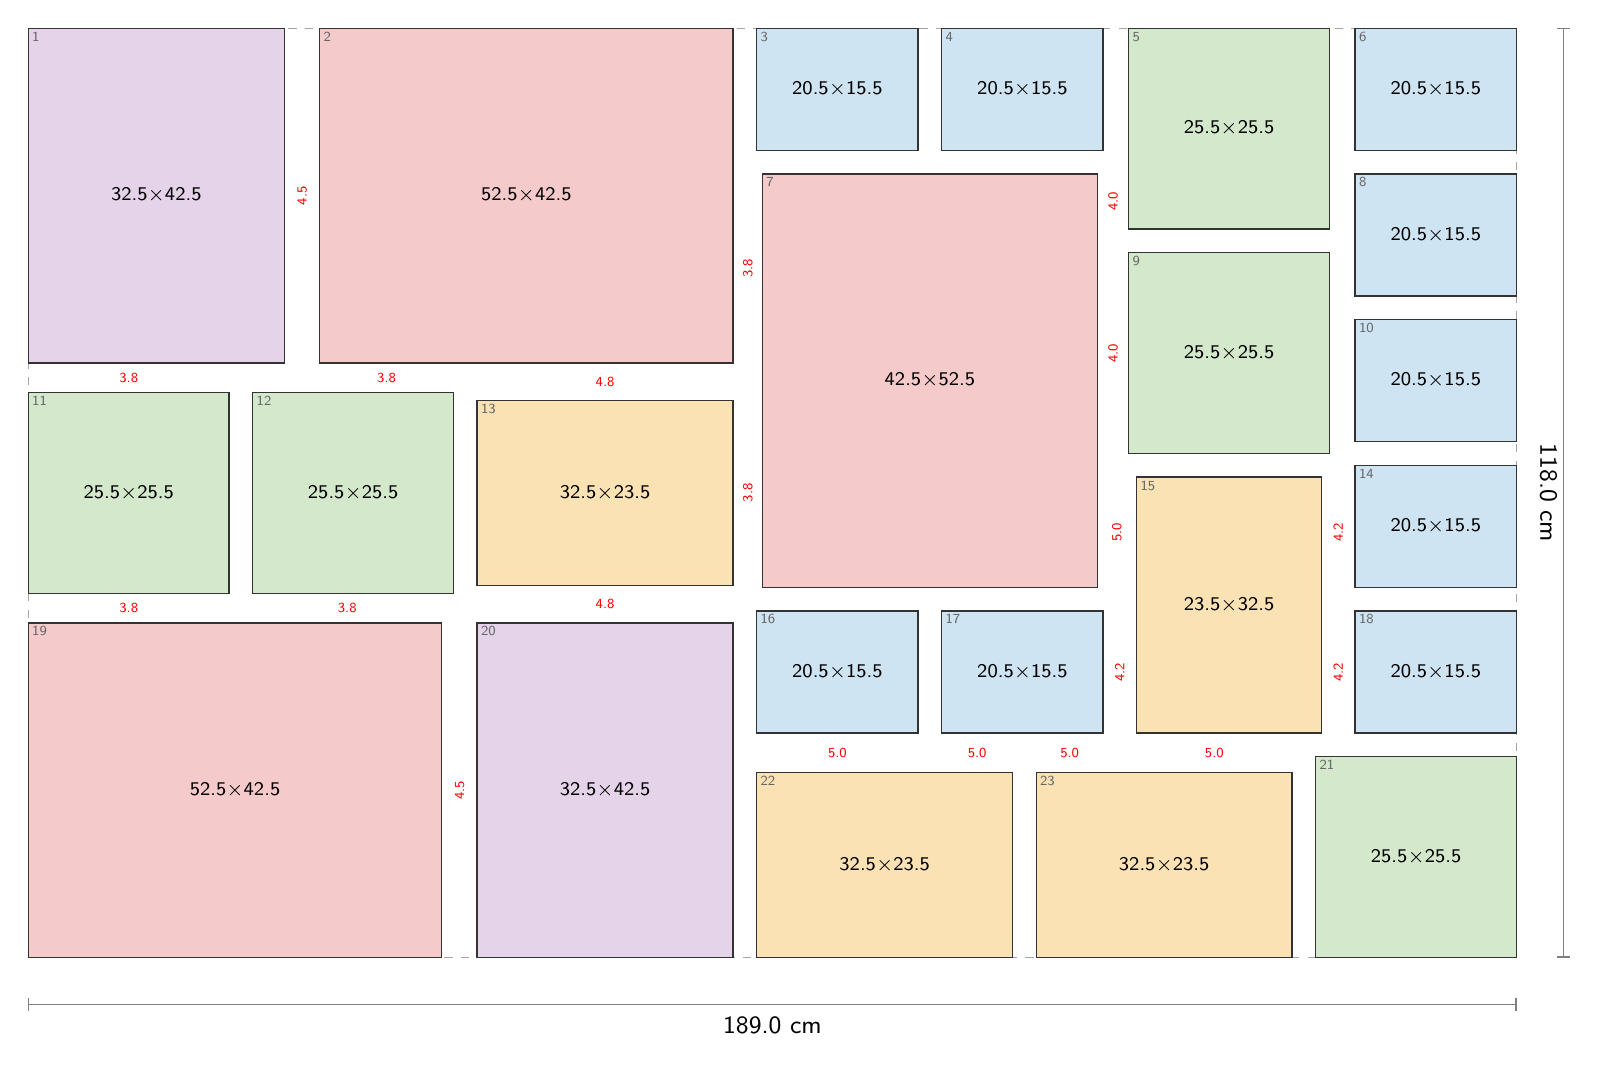
\begin{tikzpicture}[x=1mm, y=-1mm]
\draw[gray!70, dashed, line width=0.4pt] (0,0) rectangle (189.00,118.00);
\filldraw[fill=ft3, draw=black!80, line width=0.5pt] (0.00,0.00) rectangle (32.50,42.50);
\node[align=center, inner sep=0pt] at (16.25,21.25) {\scriptsize 32.5$\times$42.5};
\node[anchor=north west, inner sep=1.2pt, font=\tiny, text=black!60] at (0.00,0.00) {1};
\filldraw[fill=ft4, draw=black!80, line width=0.5pt] (37.00,0.00) rectangle (89.50,42.50);
\node[align=center, inner sep=0pt] at (63.25,21.25) {\scriptsize 52.5$\times$42.5};
\node[anchor=north west, inner sep=1.2pt, font=\tiny, text=black!60] at (37.00,0.00) {2};
\filldraw[fill=ft0, draw=black!80, line width=0.5pt] (92.50,0.00) rectangle (113.00,15.50);
\node[align=center, inner sep=0pt] at (102.75,7.75) {\scriptsize 20.5$\times$15.5};
\node[anchor=north west, inner sep=1.2pt, font=\tiny, text=black!60] at (92.50,0.00) {3};
\filldraw[fill=ft0, draw=black!80, line width=0.5pt] (116.00,0.00) rectangle (136.50,15.50);
\node[align=center, inner sep=0pt] at (126.25,7.75) {\scriptsize 20.5$\times$15.5};
\node[anchor=north west, inner sep=1.2pt, font=\tiny, text=black!60] at (116.00,0.00) {4};
\filldraw[fill=ft2, draw=black!80, line width=0.5pt] (139.75,0.00) rectangle (165.25,25.50);
\node[align=center, inner sep=0pt] at (152.50,12.75) {\scriptsize 25.5$\times$25.5};
\node[anchor=north west, inner sep=1.2pt, font=\tiny, text=black!60] at (139.75,0.00) {5};
\filldraw[fill=ft0, draw=black!80, line width=0.5pt] (168.50,0.00) rectangle (189.00,15.50);
\node[align=center, inner sep=0pt] at (178.75,7.75) {\scriptsize 20.5$\times$15.5};
\node[anchor=north west, inner sep=1.2pt, font=\tiny, text=black!60] at (168.50,0.00) {6};
\filldraw[fill=ft4, draw=black!80, line width=0.5pt] (93.25,18.50) rectangle (135.75,71.00);
\node[align=center, inner sep=0pt] at (114.50,44.75) {\scriptsize 42.5$\times$52.5};
\node[anchor=north west, inner sep=1.2pt, font=\tiny, text=black!60] at (93.25,18.50) {7};
\filldraw[fill=ft0, draw=black!80, line width=0.5pt] (168.50,18.50) rectangle (189.00,34.00);
\node[align=center, inner sep=0pt] at (178.75,26.25) {\scriptsize 20.5$\times$15.5};
\node[anchor=north west, inner sep=1.2pt, font=\tiny, text=black!60] at (168.50,18.50) {8};
\filldraw[fill=ft2, draw=black!80, line width=0.5pt] (139.75,28.50) rectangle (165.25,54.00);
\node[align=center, inner sep=0pt] at (152.50,41.25) {\scriptsize 25.5$\times$25.5};
\node[anchor=north west, inner sep=1.2pt, font=\tiny, text=black!60] at (139.75,28.50) {9};
\filldraw[fill=ft0, draw=black!80, line width=0.5pt] (168.50,37.00) rectangle (189.00,52.50);
\node[align=center, inner sep=0pt] at (178.75,44.75) {\scriptsize 20.5$\times$15.5};
\node[anchor=north west, inner sep=1.2pt, font=\tiny, text=black!60] at (168.50,37.00) {10};
\filldraw[fill=ft2, draw=black!80, line width=0.5pt] (0.00,46.25) rectangle (25.50,71.75);
\node[align=center, inner sep=0pt] at (12.75,59.00) {\scriptsize 25.5$\times$25.5};
\node[anchor=north west, inner sep=1.2pt, font=\tiny, text=black!60] at (0.00,46.25) {11};
\filldraw[fill=ft2, draw=black!80, line width=0.5pt] (28.50,46.25) rectangle (54.00,71.75);
\node[align=center, inner sep=0pt] at (41.25,59.00) {\scriptsize 25.5$\times$25.5};
\node[anchor=north west, inner sep=1.2pt, font=\tiny, text=black!60] at (28.50,46.25) {12};
\filldraw[fill=ft1, draw=black!80, line width=0.5pt] (57.00,47.25) rectangle (89.50,70.75);
\node[align=center, inner sep=0pt] at (73.25,59.00) {\scriptsize 32.5$\times$23.5};
\node[anchor=north west, inner sep=1.2pt, font=\tiny, text=black!60] at (57.00,47.25) {13};
\filldraw[fill=ft0, draw=black!80, line width=0.5pt] (168.50,55.50) rectangle (189.00,71.00);
\node[align=center, inner sep=0pt] at (178.75,63.25) {\scriptsize 20.5$\times$15.5};
\node[anchor=north west, inner sep=1.2pt, font=\tiny, text=black!60] at (168.50,55.50) {14};
\filldraw[fill=ft1, draw=black!80, line width=0.5pt] (140.75,57.00) rectangle (164.25,89.50);
\node[align=center, inner sep=0pt] at (152.50,73.25) {\scriptsize 23.5$\times$32.5};
\node[anchor=north west, inner sep=1.2pt, font=\tiny, text=black!60] at (140.75,57.00) {15};
\filldraw[fill=ft0, draw=black!80, line width=0.5pt] (92.50,74.00) rectangle (113.00,89.50);
\node[align=center, inner sep=0pt] at (102.75,81.75) {\scriptsize 20.5$\times$15.5};
\node[anchor=north west, inner sep=1.2pt, font=\tiny, text=black!60] at (92.50,74.00) {16};
\filldraw[fill=ft0, draw=black!80, line width=0.5pt] (116.00,74.00) rectangle (136.50,89.50);
\node[align=center, inner sep=0pt] at (126.25,81.75) {\scriptsize 20.5$\times$15.5};
\node[anchor=north west, inner sep=1.2pt, font=\tiny, text=black!60] at (116.00,74.00) {17};
\filldraw[fill=ft0, draw=black!80, line width=0.5pt] (168.50,74.00) rectangle (189.00,89.50);
\node[align=center, inner sep=0pt] at (178.75,81.75) {\scriptsize 20.5$\times$15.5};
\node[anchor=north west, inner sep=1.2pt, font=\tiny, text=black!60] at (168.50,74.00) {18};
\filldraw[fill=ft4, draw=black!80, line width=0.5pt] (0.00,75.50) rectangle (52.50,118.00);
\node[align=center, inner sep=0pt] at (26.25,96.75) {\scriptsize 52.5$\times$42.5};
\node[anchor=north west, inner sep=1.2pt, font=\tiny, text=black!60] at (0.00,75.50) {19};
\filldraw[fill=ft3, draw=black!80, line width=0.5pt] (57.00,75.50) rectangle (89.50,118.00);
\node[align=center, inner sep=0pt] at (73.25,96.75) {\scriptsize 32.5$\times$42.5};
\node[anchor=north west, inner sep=1.2pt, font=\tiny, text=black!60] at (57.00,75.50) {20};
\filldraw[fill=ft2, draw=black!80, line width=0.5pt] (163.50,92.50) rectangle (189.00,118.00);
\node[align=center, inner sep=0pt] at (176.25,105.25) {\scriptsize 25.5$\times$25.5};
\node[anchor=north west, inner sep=1.2pt, font=\tiny, text=black!60] at (163.50,92.50) {21};
\filldraw[fill=ft1, draw=black!80, line width=0.5pt] (92.50,94.50) rectangle (125.00,118.00);
\node[align=center, inner sep=0pt] at (108.75,106.25) {\scriptsize 32.5$\times$23.5};
\node[anchor=north west, inner sep=1.2pt, font=\tiny, text=black!60] at (92.50,94.50) {22};
\filldraw[fill=ft1, draw=black!80, line width=0.5pt] (128.00,94.50) rectangle (160.50,118.00);
\node[align=center, inner sep=0pt] at (144.25,106.25) {\scriptsize 32.5$\times$23.5};
\node[anchor=north west, inner sep=1.2pt, font=\tiny, text=black!60] at (128.00,94.50) {23};
\node[font=\tiny, text=red, fill=white, inner sep=0.3pt, rotate=90] at (34.75,21.25) {4.5};
\node[font=\tiny, text=red, fill=white, inner sep=0.3pt] at (12.75,44.38) {3.8};
\node[font=\tiny, text=red, fill=white, inner sep=0.3pt, rotate=90] at (91.38,30.50) {3.8};
\node[font=\tiny, text=red, fill=white, inner sep=0.3pt] at (45.50,44.38) {3.8};
\node[font=\tiny, text=red, fill=white, inner sep=0.3pt] at (73.25,44.88) {4.8};
\node[font=\tiny, text=red, fill=white, inner sep=0.3pt, rotate=90] at (137.75,22.00) {4.0};
\node[font=\tiny, text=red, fill=white, inner sep=0.3pt, rotate=90] at (137.75,41.25) {4.0};
\node[font=\tiny, text=red, fill=white, inner sep=0.3pt, rotate=90] at (138.25,64.00) {5.0};
\node[font=\tiny, text=red, fill=white, inner sep=0.3pt] at (12.75,73.62) {3.8};
\node[font=\tiny, text=red, fill=white, inner sep=0.3pt] at (40.50,73.62) {3.8};
\node[font=\tiny, text=red, fill=white, inner sep=0.3pt, rotate=90] at (91.38,59.00) {3.8};
\node[font=\tiny, text=red, fill=white, inner sep=0.3pt] at (73.25,73.12) {4.8};
\node[font=\tiny, text=red, fill=white, inner sep=0.3pt, rotate=90] at (166.38,64.00) {4.2};
\node[font=\tiny, text=red, fill=white, inner sep=0.3pt, rotate=90] at (166.38,81.75) {4.2};
\node[font=\tiny, text=red, fill=white, inner sep=0.3pt] at (150.62,92.00) {5.0};
\node[font=\tiny, text=red, fill=white, inner sep=0.3pt] at (102.75,92.00) {5.0};
\node[font=\tiny, text=red, fill=white, inner sep=0.3pt, rotate=90] at (138.62,81.75) {4.2};
\node[font=\tiny, text=red, fill=white, inner sep=0.3pt] at (120.50,92.00) {5.0};
\node[font=\tiny, text=red, fill=white, inner sep=0.3pt] at (132.25,92.00) {5.0};
\node[font=\tiny, text=red, fill=white, inner sep=0.3pt, rotate=90] at (54.75,96.75) {4.5};
\draw[Bar-Bar, gray] (0,124.00) -- (189.00,124.00) node[midway, below=1pt, font=\small, text=black] {189.0 cm};
\draw[Bar-Bar, gray] (195.00,0) -- (195.00,118.00) node[midway, right=1pt, font=\small, text=black, rotate=-90, anchor=north] {118.0 cm};
\end{tikzpicture}\\[4pt]
{\scriptsize Scale 1:10 (1 mm = 1 cm). Red numbers mark gaps that deviate from the nominal gap by more than 0.25 cm. Small grey numbers index the coordinate table.}
\end{minipage}\hfill
\begin{minipage}[t]{0.25\textwidth}\vspace{0pt}
\small
\begin{tabular}{@{}l l@{}}
\toprule
Outer size & 189.0 $\times$ 118.0 cm \\
Nominal gap & 3 cm \\
Actual gaps & 3.0 -- 5.0 cm \\
Max.\ deviation & 2.0 cm \\
Mean deviation & 0.62 cm \\
Border notches & top 4 cm, bottom 4 cm \\
Corners filled & 4 / 4 \\
Frames used & 23 of 28 \\
Large frames & {\scriptsize 3, touching 1$\times$ (24 cm), min.\ dist.\ 56 cm} \\
Entropy & 0.75 \\
\quad {\scriptsize mix / variety} & {\scriptsize 0.76 / 0.73} \\
\quad {\scriptsize stagger / lines} & {\scriptsize 0.52 / 1.00 (1 through)} \\
\bottomrule
\end{tabular}

\vspace{8pt}
\scriptsize
\begin{tabular}{@{}c l l r r@{}}
\toprule
 & outer w $\times$ h (cm) &  & used & have \\
\midrule
\tikz[baseline=-0.6ex]\fill[ft0,draw=black!60] (0,0) rectangle (1.2ex,1.2ex); & 20.5$\times$15.5 & L & 9 & 9 \\
\tikz[baseline=-0.6ex]\fill[ft0,draw=black!60] (0,0) rectangle (1.2ex,1.2ex); & 15.5$\times$20.5 & P & 0 & 2 \\
\tikz[baseline=-0.6ex]\fill[ft3,draw=black!60] (0,0) rectangle (1.2ex,1.2ex); & 32.5$\times$42.5 & P & 2 & 2 \\
\tikz[baseline=-0.6ex]\fill[ft3,draw=black!60] (0,0) rectangle (1.2ex,1.2ex); & 42.5$\times$32.5 & L & 0 & 1 \\
\tikz[baseline=-0.6ex]\fill[ft1,draw=black!60] (0,0) rectangle (1.2ex,1.2ex); & 32.5$\times$23.5 & L & 3 & 5 \\
\tikz[baseline=-0.6ex]\fill[ft1,draw=black!60] (0,0) rectangle (1.2ex,1.2ex); & 23.5$\times$32.5 & P & 1 & 1 \\
\tikz[baseline=-0.6ex]\fill[ft2,draw=black!60] (0,0) rectangle (1.2ex,1.2ex); & 25.5$\times$25.5 &  & 5 & 5 \\
\tikz[baseline=-0.6ex]\fill[ft4,draw=black!60] (0,0) rectangle (1.2ex,1.2ex); & 42.5$\times$52.5 & P & 1 & 1 \\
\tikz[baseline=-0.6ex]\fill[ft4,draw=black!60] (0,0) rectangle (1.2ex,1.2ex); & 52.5$\times$42.5 & L & 2 & 2 \\
\bottomrule
\end{tabular}

\vspace{8pt}
{\bfseries Positions} (top-left corner, cm)\\[2pt]
\tiny
\begin{tabular}{@{}r l r r@{}}
\toprule
\# & frame w $\times$ h & x & y \\
\midrule
1 & 32.5 $\times$ 42.5 & 0.0 & 0.0 \\
2 & 52.5 $\times$ 42.5 & 37.0 & 0.0 \\
3 & 20.5 $\times$ 15.5 & 92.5 & 0.0 \\
4 & 20.5 $\times$ 15.5 & 116.0 & 0.0 \\
5 & 25.5 $\times$ 25.5 & 139.8 & 0.0 \\
6 & 20.5 $\times$ 15.5 & 168.5 & 0.0 \\
7 & 42.5 $\times$ 52.5 & 93.2 & 18.5 \\
8 & 20.5 $\times$ 15.5 & 168.5 & 18.5 \\
9 & 25.5 $\times$ 25.5 & 139.8 & 28.5 \\
10 & 20.5 $\times$ 15.5 & 168.5 & 37.0 \\
11 & 25.5 $\times$ 25.5 & 0.0 & 46.2 \\
12 & 25.5 $\times$ 25.5 & 28.5 & 46.2 \\
13 & 32.5 $\times$ 23.5 & 57.0 & 47.2 \\
14 & 20.5 $\times$ 15.5 & 168.5 & 55.5 \\
15 & 23.5 $\times$ 32.5 & 140.8 & 57.0 \\
16 & 20.5 $\times$ 15.5 & 92.5 & 74.0 \\
17 & 20.5 $\times$ 15.5 & 116.0 & 74.0 \\
18 & 20.5 $\times$ 15.5 & 168.5 & 74.0 \\
19 & 52.5 $\times$ 42.5 & 0.0 & 75.5 \\
20 & 32.5 $\times$ 42.5 & 57.0 & 75.5 \\
21 & 25.5 $\times$ 25.5 & 163.5 & 92.5 \\
22 & 32.5 $\times$ 23.5 & 92.5 & 94.5 \\
23 & 32.5 $\times$ 23.5 & 128.0 & 94.5 \\
\bottomrule
\end{tabular}
\end{minipage}
\clearpage

\phantomsection\addcontentsline{toc}{subsection}{Layout 9: 183.5 \texorpdfstring{$\times$}{x} 130.5 cm, 23 frames, gap 4.5 cm, max.\ deviation 3.6 cm}
\label{lay:per-run-gap:9}
\begin{minipage}[t]{0.74\textwidth}\vspace{0pt}
{\LARGE\bfseries Layout 9}\hspace{1.5em}{\large 183.5 $\times$ 130.5 cm \quad gap 4.5 cm \quad 23 frames}\\[8pt]
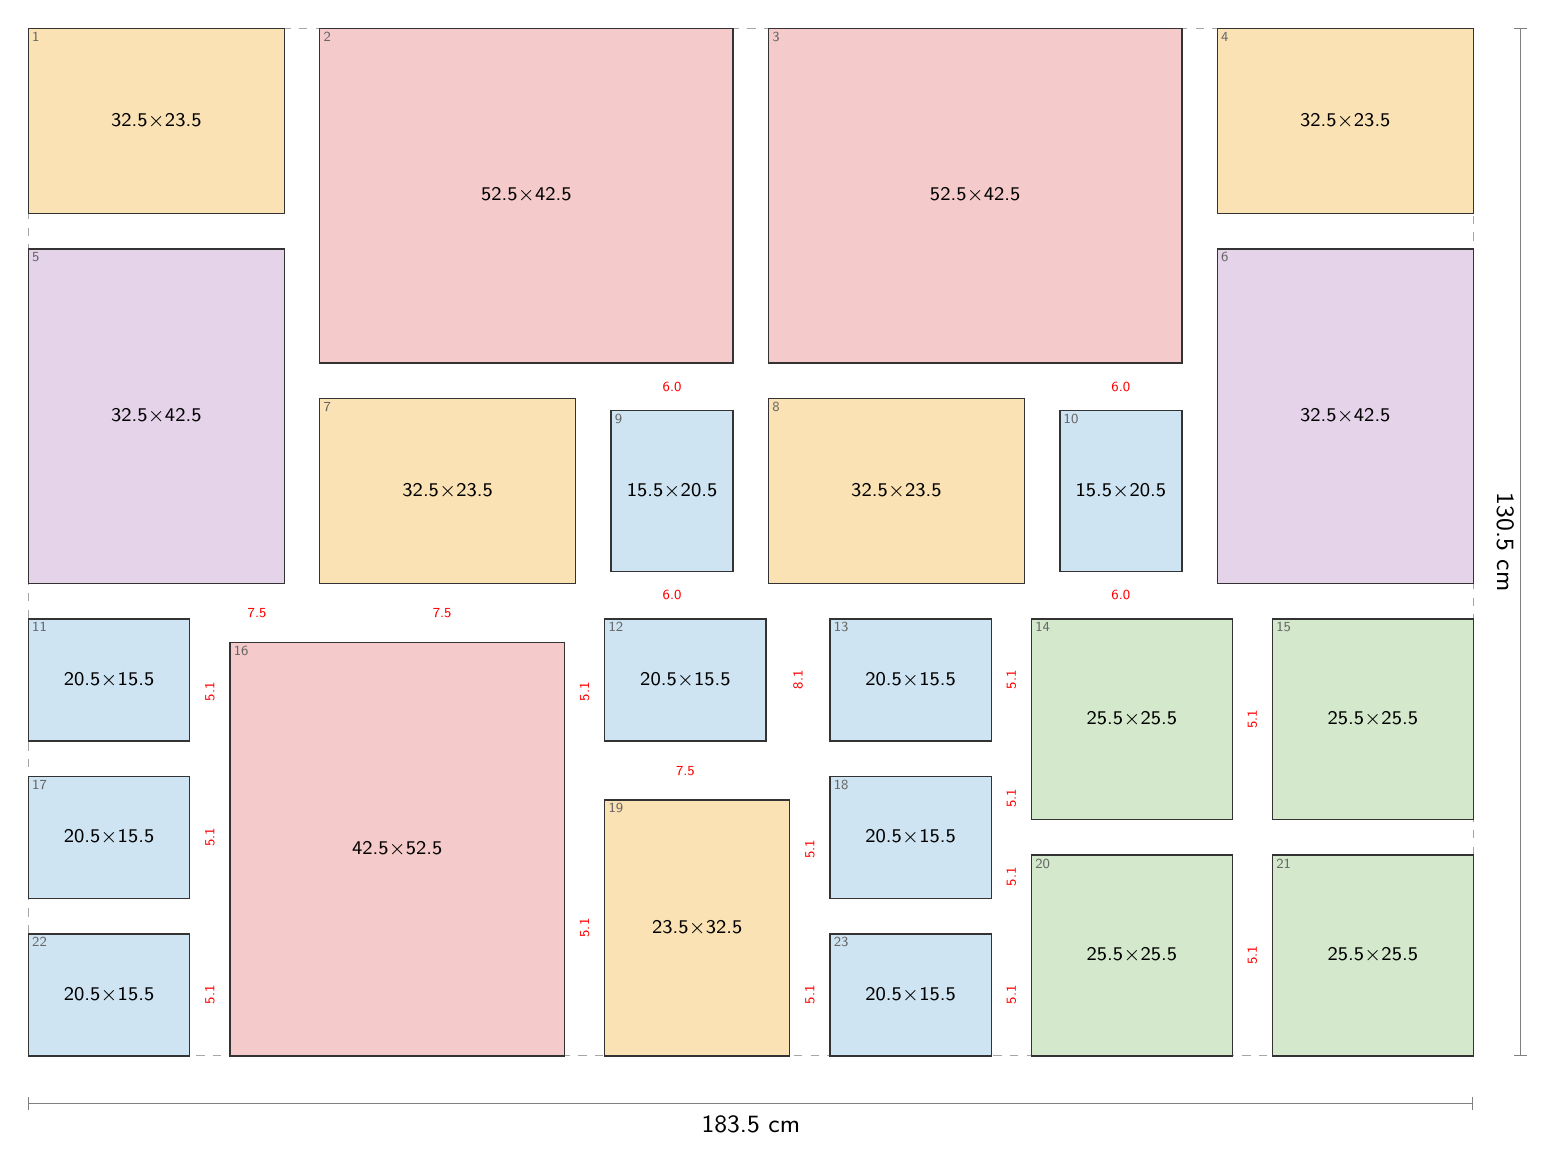
\begin{tikzpicture}[x=1mm, y=-1mm]
\draw[gray!70, dashed, line width=0.4pt] (0,0) rectangle (183.50,130.50);
\filldraw[fill=ft1, draw=black!80, line width=0.5pt] (0.00,0.00) rectangle (32.50,23.50);
\node[align=center, inner sep=0pt] at (16.25,11.75) {\scriptsize 32.5$\times$23.5};
\node[anchor=north west, inner sep=1.2pt, font=\tiny, text=black!60] at (0.00,0.00) {1};
\filldraw[fill=ft4, draw=black!80, line width=0.5pt] (37.00,0.00) rectangle (89.50,42.50);
\node[align=center, inner sep=0pt] at (63.25,21.25) {\scriptsize 52.5$\times$42.5};
\node[anchor=north west, inner sep=1.2pt, font=\tiny, text=black!60] at (37.00,0.00) {2};
\filldraw[fill=ft4, draw=black!80, line width=0.5pt] (94.00,0.00) rectangle (146.50,42.50);
\node[align=center, inner sep=0pt] at (120.25,21.25) {\scriptsize 52.5$\times$42.5};
\node[anchor=north west, inner sep=1.2pt, font=\tiny, text=black!60] at (94.00,0.00) {3};
\filldraw[fill=ft1, draw=black!80, line width=0.5pt] (151.00,0.00) rectangle (183.50,23.50);
\node[align=center, inner sep=0pt] at (167.25,11.75) {\scriptsize 32.5$\times$23.5};
\node[anchor=north west, inner sep=1.2pt, font=\tiny, text=black!60] at (151.00,0.00) {4};
\filldraw[fill=ft3, draw=black!80, line width=0.5pt] (0.00,28.00) rectangle (32.50,70.50);
\node[align=center, inner sep=0pt] at (16.25,49.25) {\scriptsize 32.5$\times$42.5};
\node[anchor=north west, inner sep=1.2pt, font=\tiny, text=black!60] at (0.00,28.00) {5};
\filldraw[fill=ft3, draw=black!80, line width=0.5pt] (151.00,28.00) rectangle (183.50,70.50);
\node[align=center, inner sep=0pt] at (167.25,49.25) {\scriptsize 32.5$\times$42.5};
\node[anchor=north west, inner sep=1.2pt, font=\tiny, text=black!60] at (151.00,28.00) {6};
\filldraw[fill=ft1, draw=black!80, line width=0.5pt] (37.00,47.00) rectangle (69.50,70.50);
\node[align=center, inner sep=0pt] at (53.25,58.75) {\scriptsize 32.5$\times$23.5};
\node[anchor=north west, inner sep=1.2pt, font=\tiny, text=black!60] at (37.00,47.00) {7};
\filldraw[fill=ft1, draw=black!80, line width=0.5pt] (94.00,47.00) rectangle (126.50,70.50);
\node[align=center, inner sep=0pt] at (110.25,58.75) {\scriptsize 32.5$\times$23.5};
\node[anchor=north west, inner sep=1.2pt, font=\tiny, text=black!60] at (94.00,47.00) {8};
\filldraw[fill=ft0, draw=black!80, line width=0.5pt] (74.00,48.50) rectangle (89.50,69.00);
\node[align=center, inner sep=0pt] at (81.75,58.75) {\scriptsize 15.5$\times$20.5};
\node[anchor=north west, inner sep=1.2pt, font=\tiny, text=black!60] at (74.00,48.50) {9};
\filldraw[fill=ft0, draw=black!80, line width=0.5pt] (131.00,48.50) rectangle (146.50,69.00);
\node[align=center, inner sep=0pt] at (138.75,58.75) {\scriptsize 15.5$\times$20.5};
\node[anchor=north west, inner sep=1.2pt, font=\tiny, text=black!60] at (131.00,48.50) {10};
\filldraw[fill=ft0, draw=black!80, line width=0.5pt] (0.00,75.00) rectangle (20.50,90.50);
\node[align=center, inner sep=0pt] at (10.25,82.75) {\scriptsize 20.5$\times$15.5};
\node[anchor=north west, inner sep=1.2pt, font=\tiny, text=black!60] at (0.00,75.00) {11};
\filldraw[fill=ft0, draw=black!80, line width=0.5pt] (73.20,75.00) rectangle (93.70,90.50);
\node[align=center, inner sep=0pt] at (83.45,82.75) {\scriptsize 20.5$\times$15.5};
\node[anchor=north west, inner sep=1.2pt, font=\tiny, text=black!60] at (73.20,75.00) {12};
\filldraw[fill=ft0, draw=black!80, line width=0.5pt] (101.80,75.00) rectangle (122.30,90.50);
\node[align=center, inner sep=0pt] at (112.05,82.75) {\scriptsize 20.5$\times$15.5};
\node[anchor=north west, inner sep=1.2pt, font=\tiny, text=black!60] at (101.80,75.00) {13};
\filldraw[fill=ft2, draw=black!80, line width=0.5pt] (127.40,75.00) rectangle (152.90,100.50);
\node[align=center, inner sep=0pt] at (140.15,87.75) {\scriptsize 25.5$\times$25.5};
\node[anchor=north west, inner sep=1.2pt, font=\tiny, text=black!60] at (127.40,75.00) {14};
\filldraw[fill=ft2, draw=black!80, line width=0.5pt] (158.00,75.00) rectangle (183.50,100.50);
\node[align=center, inner sep=0pt] at (170.75,87.75) {\scriptsize 25.5$\times$25.5};
\node[anchor=north west, inner sep=1.2pt, font=\tiny, text=black!60] at (158.00,75.00) {15};
\filldraw[fill=ft4, draw=black!80, line width=0.5pt] (25.60,78.00) rectangle (68.10,130.50);
\node[align=center, inner sep=0pt] at (46.85,104.25) {\scriptsize 42.5$\times$52.5};
\node[anchor=north west, inner sep=1.2pt, font=\tiny, text=black!60] at (25.60,78.00) {16};
\filldraw[fill=ft0, draw=black!80, line width=0.5pt] (0.00,95.00) rectangle (20.50,110.50);
\node[align=center, inner sep=0pt] at (10.25,102.75) {\scriptsize 20.5$\times$15.5};
\node[anchor=north west, inner sep=1.2pt, font=\tiny, text=black!60] at (0.00,95.00) {17};
\filldraw[fill=ft0, draw=black!80, line width=0.5pt] (101.80,95.00) rectangle (122.30,110.50);
\node[align=center, inner sep=0pt] at (112.05,102.75) {\scriptsize 20.5$\times$15.5};
\node[anchor=north west, inner sep=1.2pt, font=\tiny, text=black!60] at (101.80,95.00) {18};
\filldraw[fill=ft1, draw=black!80, line width=0.5pt] (73.20,98.00) rectangle (96.70,130.50);
\node[align=center, inner sep=0pt] at (84.95,114.25) {\scriptsize 23.5$\times$32.5};
\node[anchor=north west, inner sep=1.2pt, font=\tiny, text=black!60] at (73.20,98.00) {19};
\filldraw[fill=ft2, draw=black!80, line width=0.5pt] (127.40,105.00) rectangle (152.90,130.50);
\node[align=center, inner sep=0pt] at (140.15,117.75) {\scriptsize 25.5$\times$25.5};
\node[anchor=north west, inner sep=1.2pt, font=\tiny, text=black!60] at (127.40,105.00) {20};
\filldraw[fill=ft2, draw=black!80, line width=0.5pt] (158.00,105.00) rectangle (183.50,130.50);
\node[align=center, inner sep=0pt] at (170.75,117.75) {\scriptsize 25.5$\times$25.5};
\node[anchor=north west, inner sep=1.2pt, font=\tiny, text=black!60] at (158.00,105.00) {21};
\filldraw[fill=ft0, draw=black!80, line width=0.5pt] (0.00,115.00) rectangle (20.50,130.50);
\node[align=center, inner sep=0pt] at (10.25,122.75) {\scriptsize 20.5$\times$15.5};
\node[anchor=north west, inner sep=1.2pt, font=\tiny, text=black!60] at (0.00,115.00) {22};
\filldraw[fill=ft0, draw=black!80, line width=0.5pt] (101.80,115.00) rectangle (122.30,130.50);
\node[align=center, inner sep=0pt] at (112.05,122.75) {\scriptsize 20.5$\times$15.5};
\node[anchor=north west, inner sep=1.2pt, font=\tiny, text=black!60] at (101.80,115.00) {23};
\node[font=\tiny, text=red, fill=white, inner sep=0.3pt] at (81.75,45.50) {6.0};
\node[font=\tiny, text=red, fill=white, inner sep=0.3pt] at (138.75,45.50) {6.0};
\node[font=\tiny, text=red, fill=white, inner sep=0.3pt] at (29.05,74.25) {7.5};
\node[font=\tiny, text=red, fill=white, inner sep=0.3pt] at (52.55,74.25) {7.5};
\node[font=\tiny, text=red, fill=white, inner sep=0.3pt] at (81.75,72.00) {6.0};
\node[font=\tiny, text=red, fill=white, inner sep=0.3pt] at (138.75,72.00) {6.0};
\node[font=\tiny, text=red, fill=white, inner sep=0.3pt, rotate=90] at (23.05,84.25) {5.1};
\node[font=\tiny, text=red, fill=white, inner sep=0.3pt, rotate=90] at (97.75,82.75) {8.1};
\node[font=\tiny, text=red, fill=white, inner sep=0.3pt] at (83.45,94.25) {7.5};
\node[font=\tiny, text=red, fill=white, inner sep=0.3pt, rotate=90] at (124.85,82.75) {5.1};
\node[font=\tiny, text=red, fill=white, inner sep=0.3pt, rotate=90] at (155.45,87.75) {5.1};
\node[font=\tiny, text=red, fill=white, inner sep=0.3pt, rotate=90] at (70.65,84.25) {5.1};
\node[font=\tiny, text=red, fill=white, inner sep=0.3pt, rotate=90] at (70.65,114.25) {5.1};
\node[font=\tiny, text=red, fill=white, inner sep=0.3pt, rotate=90] at (23.05,102.75) {5.1};
\node[font=\tiny, text=red, fill=white, inner sep=0.3pt, rotate=90] at (124.85,97.75) {5.1};
\node[font=\tiny, text=red, fill=white, inner sep=0.3pt, rotate=90] at (124.85,107.75) {5.1};
\node[font=\tiny, text=red, fill=white, inner sep=0.3pt, rotate=90] at (99.25,104.25) {5.1};
\node[font=\tiny, text=red, fill=white, inner sep=0.3pt, rotate=90] at (99.25,122.75) {5.1};
\node[font=\tiny, text=red, fill=white, inner sep=0.3pt, rotate=90] at (155.45,117.75) {5.1};
\node[font=\tiny, text=red, fill=white, inner sep=0.3pt, rotate=90] at (23.05,122.75) {5.1};
\node[font=\tiny, text=red, fill=white, inner sep=0.3pt, rotate=90] at (124.85,122.75) {5.1};
\draw[Bar-Bar, gray] (0,136.50) -- (183.50,136.50) node[midway, below=1pt, font=\small, text=black] {183.5 cm};
\draw[Bar-Bar, gray] (189.50,0) -- (189.50,130.50) node[midway, right=1pt, font=\small, text=black, rotate=-90, anchor=north] {130.5 cm};
\end{tikzpicture}\\[4pt]
{\scriptsize Scale 1:10 (1 mm = 1 cm). Red numbers mark gaps that deviate from the nominal gap by more than 0.25 cm. Small grey numbers index the coordinate table.}
\end{minipage}\hfill
\begin{minipage}[t]{0.25\textwidth}\vspace{0pt}
\small
\begin{tabular}{@{}l l@{}}
\toprule
Outer size & 183.5 $\times$ 130.5 cm \\
Nominal gap & 4.5 cm \\
Actual gaps & 4.5 -- 8.1 cm \\
Max.\ deviation & 3.6 cm \\
Mean deviation & 0.60 cm \\
Border notches & none \\
Corners filled & 4 / 4 \\
Frames used & 23 of 28 \\
Large frames & {\scriptsize 3, touching 1$\times$ (42 cm), min.\ dist.\ 57 cm} \\
Entropy & 0.76 \\
\quad {\scriptsize mix / variety} & {\scriptsize 0.86 / 0.75} \\
\quad {\scriptsize stagger / lines} & {\scriptsize 0.45 / 1.00 (1 through)} \\
\bottomrule
\end{tabular}

\vspace{8pt}
\scriptsize
\begin{tabular}{@{}c l l r r@{}}
\toprule
 & outer w $\times$ h (cm) &  & used & have \\
\midrule
\tikz[baseline=-0.6ex]\fill[ft0,draw=black!60] (0,0) rectangle (1.2ex,1.2ex); & 20.5$\times$15.5 & L & 7 & 9 \\
\tikz[baseline=-0.6ex]\fill[ft0,draw=black!60] (0,0) rectangle (1.2ex,1.2ex); & 15.5$\times$20.5 & P & 2 & 2 \\
\tikz[baseline=-0.6ex]\fill[ft3,draw=black!60] (0,0) rectangle (1.2ex,1.2ex); & 32.5$\times$42.5 & P & 2 & 2 \\
\tikz[baseline=-0.6ex]\fill[ft3,draw=black!60] (0,0) rectangle (1.2ex,1.2ex); & 42.5$\times$32.5 & L & 0 & 1 \\
\tikz[baseline=-0.6ex]\fill[ft1,draw=black!60] (0,0) rectangle (1.2ex,1.2ex); & 32.5$\times$23.5 & L & 4 & 5 \\
\tikz[baseline=-0.6ex]\fill[ft1,draw=black!60] (0,0) rectangle (1.2ex,1.2ex); & 23.5$\times$32.5 & P & 1 & 1 \\
\tikz[baseline=-0.6ex]\fill[ft2,draw=black!60] (0,0) rectangle (1.2ex,1.2ex); & 25.5$\times$25.5 &  & 4 & 5 \\
\tikz[baseline=-0.6ex]\fill[ft4,draw=black!60] (0,0) rectangle (1.2ex,1.2ex); & 42.5$\times$52.5 & P & 1 & 1 \\
\tikz[baseline=-0.6ex]\fill[ft4,draw=black!60] (0,0) rectangle (1.2ex,1.2ex); & 52.5$\times$42.5 & L & 2 & 2 \\
\bottomrule
\end{tabular}

\vspace{8pt}
{\bfseries Positions} (top-left corner, cm)\\[2pt]
\tiny
\begin{tabular}{@{}r l r r@{}}
\toprule
\# & frame w $\times$ h & x & y \\
\midrule
1 & 32.5 $\times$ 23.5 & 0.0 & 0.0 \\
2 & 52.5 $\times$ 42.5 & 37.0 & 0.0 \\
3 & 52.5 $\times$ 42.5 & 94.0 & 0.0 \\
4 & 32.5 $\times$ 23.5 & 151.0 & 0.0 \\
5 & 32.5 $\times$ 42.5 & 0.0 & 28.0 \\
6 & 32.5 $\times$ 42.5 & 151.0 & 28.0 \\
7 & 32.5 $\times$ 23.5 & 37.0 & 47.0 \\
8 & 32.5 $\times$ 23.5 & 94.0 & 47.0 \\
9 & 15.5 $\times$ 20.5 & 74.0 & 48.5 \\
10 & 15.5 $\times$ 20.5 & 131.0 & 48.5 \\
11 & 20.5 $\times$ 15.5 & 0.0 & 75.0 \\
12 & 20.5 $\times$ 15.5 & 73.2 & 75.0 \\
13 & 20.5 $\times$ 15.5 & 101.8 & 75.0 \\
14 & 25.5 $\times$ 25.5 & 127.4 & 75.0 \\
15 & 25.5 $\times$ 25.5 & 158.0 & 75.0 \\
16 & 42.5 $\times$ 52.5 & 25.6 & 78.0 \\
17 & 20.5 $\times$ 15.5 & 0.0 & 95.0 \\
18 & 20.5 $\times$ 15.5 & 101.8 & 95.0 \\
19 & 23.5 $\times$ 32.5 & 73.2 & 98.0 \\
20 & 25.5 $\times$ 25.5 & 127.4 & 105.0 \\
21 & 25.5 $\times$ 25.5 & 158.0 & 105.0 \\
22 & 20.5 $\times$ 15.5 & 0.0 & 115.0 \\
23 & 20.5 $\times$ 15.5 & 101.8 & 115.0 \\
\bottomrule
\end{tabular}
\end{minipage}
\clearpage

\phantomsection\addcontentsline{toc}{subsection}{Layout 10: 189.0 \texorpdfstring{$\times$}{x} 119.0 cm, 22 frames, gap 5 cm, max.\ deviation 3.5 cm}
\label{lay:per-run-gap:10}
\begin{minipage}[t]{0.74\textwidth}\vspace{0pt}
{\LARGE\bfseries Layout 10}\hspace{1.5em}{\large 189.0 $\times$ 119.0 cm \quad gap 5 cm \quad 22 frames}\\[8pt]
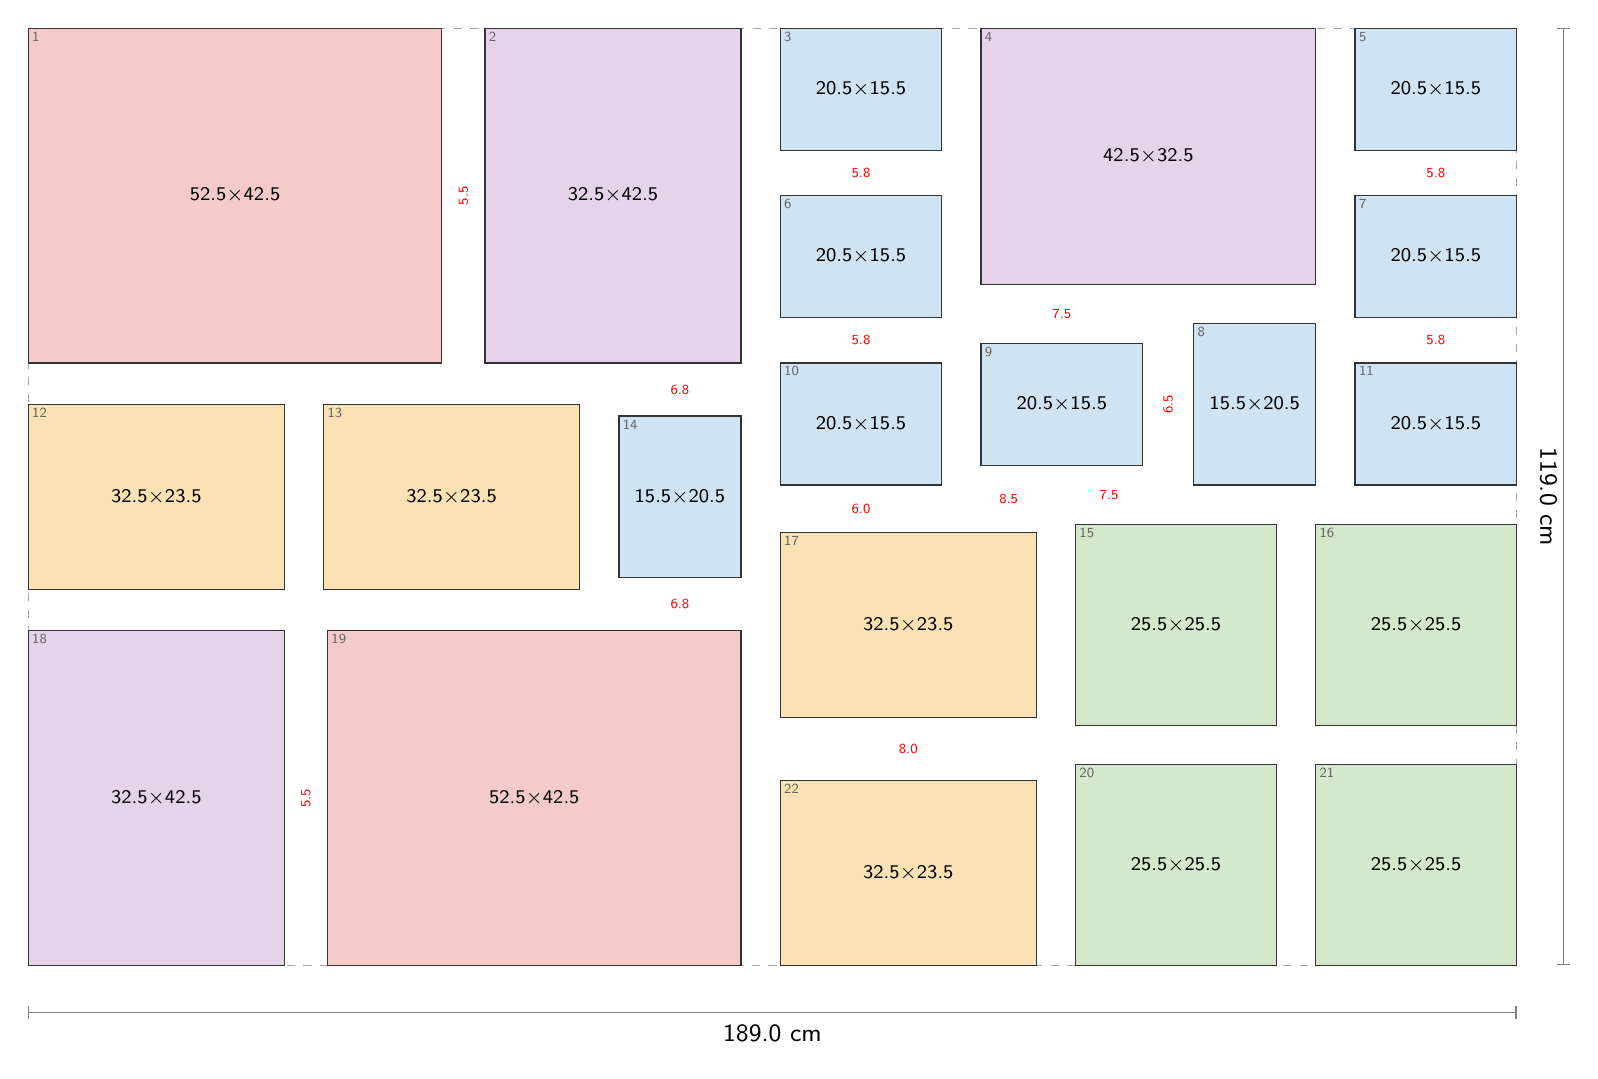
\begin{tikzpicture}[x=1mm, y=-1mm]
\draw[gray!70, dashed, line width=0.4pt] (0,0) rectangle (189.00,119.00);
\filldraw[fill=ft4, draw=black!80, line width=0.5pt] (0.00,0.00) rectangle (52.50,42.50);
\node[align=center, inner sep=0pt] at (26.25,21.25) {\scriptsize 52.5$\times$42.5};
\node[anchor=north west, inner sep=1.2pt, font=\tiny, text=black!60] at (0.00,0.00) {1};
\filldraw[fill=ft3, draw=black!80, line width=0.5pt] (58.00,0.00) rectangle (90.50,42.50);
\node[align=center, inner sep=0pt] at (74.25,21.25) {\scriptsize 32.5$\times$42.5};
\node[anchor=north west, inner sep=1.2pt, font=\tiny, text=black!60] at (58.00,0.00) {2};
\filldraw[fill=ft0, draw=black!80, line width=0.5pt] (95.50,0.00) rectangle (116.00,15.50);
\node[align=center, inner sep=0pt] at (105.75,7.75) {\scriptsize 20.5$\times$15.5};
\node[anchor=north west, inner sep=1.2pt, font=\tiny, text=black!60] at (95.50,0.00) {3};
\filldraw[fill=ft3, draw=black!80, line width=0.5pt] (121.00,0.00) rectangle (163.50,32.50);
\node[align=center, inner sep=0pt] at (142.25,16.25) {\scriptsize 42.5$\times$32.5};
\node[anchor=north west, inner sep=1.2pt, font=\tiny, text=black!60] at (121.00,0.00) {4};
\filldraw[fill=ft0, draw=black!80, line width=0.5pt] (168.50,0.00) rectangle (189.00,15.50);
\node[align=center, inner sep=0pt] at (178.75,7.75) {\scriptsize 20.5$\times$15.5};
\node[anchor=north west, inner sep=1.2pt, font=\tiny, text=black!60] at (168.50,0.00) {5};
\filldraw[fill=ft0, draw=black!80, line width=0.5pt] (95.50,21.25) rectangle (116.00,36.75);
\node[align=center, inner sep=0pt] at (105.75,29.00) {\scriptsize 20.5$\times$15.5};
\node[anchor=north west, inner sep=1.2pt, font=\tiny, text=black!60] at (95.50,21.25) {6};
\filldraw[fill=ft0, draw=black!80, line width=0.5pt] (168.50,21.25) rectangle (189.00,36.75);
\node[align=center, inner sep=0pt] at (178.75,29.00) {\scriptsize 20.5$\times$15.5};
\node[anchor=north west, inner sep=1.2pt, font=\tiny, text=black!60] at (168.50,21.25) {7};
\filldraw[fill=ft0, draw=black!80, line width=0.5pt] (148.00,37.50) rectangle (163.50,58.00);
\node[align=center, inner sep=0pt] at (155.75,47.75) {\scriptsize 15.5$\times$20.5};
\node[anchor=north west, inner sep=1.2pt, font=\tiny, text=black!60] at (148.00,37.50) {8};
\filldraw[fill=ft0, draw=black!80, line width=0.5pt] (121.00,40.00) rectangle (141.50,55.50);
\node[align=center, inner sep=0pt] at (131.25,47.75) {\scriptsize 20.5$\times$15.5};
\node[anchor=north west, inner sep=1.2pt, font=\tiny, text=black!60] at (121.00,40.00) {9};
\filldraw[fill=ft0, draw=black!80, line width=0.5pt] (95.50,42.50) rectangle (116.00,58.00);
\node[align=center, inner sep=0pt] at (105.75,50.25) {\scriptsize 20.5$\times$15.5};
\node[anchor=north west, inner sep=1.2pt, font=\tiny, text=black!60] at (95.50,42.50) {10};
\filldraw[fill=ft0, draw=black!80, line width=0.5pt] (168.50,42.50) rectangle (189.00,58.00);
\node[align=center, inner sep=0pt] at (178.75,50.25) {\scriptsize 20.5$\times$15.5};
\node[anchor=north west, inner sep=1.2pt, font=\tiny, text=black!60] at (168.50,42.50) {11};
\filldraw[fill=ft1, draw=black!80, line width=0.5pt] (0.00,47.75) rectangle (32.50,71.25);
\node[align=center, inner sep=0pt] at (16.25,59.50) {\scriptsize 32.5$\times$23.5};
\node[anchor=north west, inner sep=1.2pt, font=\tiny, text=black!60] at (0.00,47.75) {12};
\filldraw[fill=ft1, draw=black!80, line width=0.5pt] (37.50,47.75) rectangle (70.00,71.25);
\node[align=center, inner sep=0pt] at (53.75,59.50) {\scriptsize 32.5$\times$23.5};
\node[anchor=north west, inner sep=1.2pt, font=\tiny, text=black!60] at (37.50,47.75) {13};
\filldraw[fill=ft0, draw=black!80, line width=0.5pt] (75.00,49.25) rectangle (90.50,69.75);
\node[align=center, inner sep=0pt] at (82.75,59.50) {\scriptsize 15.5$\times$20.5};
\node[anchor=north west, inner sep=1.2pt, font=\tiny, text=black!60] at (75.00,49.25) {14};
\filldraw[fill=ft2, draw=black!80, line width=0.5pt] (133.00,63.00) rectangle (158.50,88.50);
\node[align=center, inner sep=0pt] at (145.75,75.75) {\scriptsize 25.5$\times$25.5};
\node[anchor=north west, inner sep=1.2pt, font=\tiny, text=black!60] at (133.00,63.00) {15};
\filldraw[fill=ft2, draw=black!80, line width=0.5pt] (163.50,63.00) rectangle (189.00,88.50);
\node[align=center, inner sep=0pt] at (176.25,75.75) {\scriptsize 25.5$\times$25.5};
\node[anchor=north west, inner sep=1.2pt, font=\tiny, text=black!60] at (163.50,63.00) {16};
\filldraw[fill=ft1, draw=black!80, line width=0.5pt] (95.50,64.00) rectangle (128.00,87.50);
\node[align=center, inner sep=0pt] at (111.75,75.75) {\scriptsize 32.5$\times$23.5};
\node[anchor=north west, inner sep=1.2pt, font=\tiny, text=black!60] at (95.50,64.00) {17};
\filldraw[fill=ft3, draw=black!80, line width=0.5pt] (0.00,76.50) rectangle (32.50,119.00);
\node[align=center, inner sep=0pt] at (16.25,97.75) {\scriptsize 32.5$\times$42.5};
\node[anchor=north west, inner sep=1.2pt, font=\tiny, text=black!60] at (0.00,76.50) {18};
\filldraw[fill=ft4, draw=black!80, line width=0.5pt] (38.00,76.50) rectangle (90.50,119.00);
\node[align=center, inner sep=0pt] at (64.25,97.75) {\scriptsize 52.5$\times$42.5};
\node[anchor=north west, inner sep=1.2pt, font=\tiny, text=black!60] at (38.00,76.50) {19};
\filldraw[fill=ft2, draw=black!80, line width=0.5pt] (133.00,93.50) rectangle (158.50,119.00);
\node[align=center, inner sep=0pt] at (145.75,106.25) {\scriptsize 25.5$\times$25.5};
\node[anchor=north west, inner sep=1.2pt, font=\tiny, text=black!60] at (133.00,93.50) {20};
\filldraw[fill=ft2, draw=black!80, line width=0.5pt] (163.50,93.50) rectangle (189.00,119.00);
\node[align=center, inner sep=0pt] at (176.25,106.25) {\scriptsize 25.5$\times$25.5};
\node[anchor=north west, inner sep=1.2pt, font=\tiny, text=black!60] at (163.50,93.50) {21};
\filldraw[fill=ft1, draw=black!80, line width=0.5pt] (95.50,95.50) rectangle (128.00,119.00);
\node[align=center, inner sep=0pt] at (111.75,107.25) {\scriptsize 32.5$\times$23.5};
\node[anchor=north west, inner sep=1.2pt, font=\tiny, text=black!60] at (95.50,95.50) {22};
\node[font=\tiny, text=red, fill=white, inner sep=0.3pt, rotate=90] at (55.25,21.25) {5.5};
\node[font=\tiny, text=red, fill=white, inner sep=0.3pt] at (82.75,45.88) {6.8};
\node[font=\tiny, text=red, fill=white, inner sep=0.3pt] at (105.75,18.38) {5.8};
\node[font=\tiny, text=red, fill=white, inner sep=0.3pt] at (131.25,36.25) {7.5};
\node[font=\tiny, text=red, fill=white, inner sep=0.3pt] at (178.75,18.38) {5.8};
\node[font=\tiny, text=red, fill=white, inner sep=0.3pt] at (105.75,39.62) {5.8};
\node[font=\tiny, text=red, fill=white, inner sep=0.3pt] at (178.75,39.62) {5.8};
\node[font=\tiny, text=red, fill=white, inner sep=0.3pt, rotate=90] at (144.75,47.75) {6.5};
\node[font=\tiny, text=red, fill=white, inner sep=0.3pt] at (137.25,59.25) {7.5};
\node[font=\tiny, text=red, fill=white, inner sep=0.3pt] at (124.50,59.75) {8.5};
\node[font=\tiny, text=red, fill=white, inner sep=0.3pt] at (105.75,61.00) {6.0};
\node[font=\tiny, text=red, fill=white, inner sep=0.3pt] at (82.75,73.12) {6.8};
\node[font=\tiny, text=red, fill=white, inner sep=0.3pt] at (111.75,91.50) {8.0};
\node[font=\tiny, text=red, fill=white, inner sep=0.3pt, rotate=90] at (35.25,97.75) {5.5};
\draw[Bar-Bar, gray] (0,125.00) -- (189.00,125.00) node[midway, below=1pt, font=\small, text=black] {189.0 cm};
\draw[Bar-Bar, gray] (195.00,0) -- (195.00,119.00) node[midway, right=1pt, font=\small, text=black, rotate=-90, anchor=north] {119.0 cm};
\end{tikzpicture}\\[4pt]
{\scriptsize Scale 1:10 (1 mm = 1 cm). Red numbers mark gaps that deviate from the nominal gap by more than 0.25 cm. Small grey numbers index the coordinate table.}
\end{minipage}\hfill
\begin{minipage}[t]{0.25\textwidth}\vspace{0pt}
\small
\begin{tabular}{@{}l l@{}}
\toprule
Outer size & 189.0 $\times$ 119.0 cm \\
Nominal gap & 5 cm \\
Actual gaps & 5.0 -- 8.5 cm \\
Max.\ deviation & 3.5 cm \\
Mean deviation & 0.54 cm \\
Border notches & none \\
Corners filled & 4 / 4 \\
Frames used & 22 of 28 \\
Large frames & {\scriptsize 2, not touching, min.\ dist.\ 85 cm} \\
Entropy & 0.75 \\
\quad {\scriptsize mix / variety} & {\scriptsize 0.81 / 0.71} \\
\quad {\scriptsize stagger / lines} & {\scriptsize 0.48 / 1.00 (1 through)} \\
\bottomrule
\end{tabular}

\vspace{8pt}
\scriptsize
\begin{tabular}{@{}c l l r r@{}}
\toprule
 & outer w $\times$ h (cm) &  & used & have \\
\midrule
\tikz[baseline=-0.6ex]\fill[ft0,draw=black!60] (0,0) rectangle (1.2ex,1.2ex); & 20.5$\times$15.5 & L & 7 & 9 \\
\tikz[baseline=-0.6ex]\fill[ft0,draw=black!60] (0,0) rectangle (1.2ex,1.2ex); & 15.5$\times$20.5 & P & 2 & 2 \\
\tikz[baseline=-0.6ex]\fill[ft3,draw=black!60] (0,0) rectangle (1.2ex,1.2ex); & 32.5$\times$42.5 & P & 2 & 2 \\
\tikz[baseline=-0.6ex]\fill[ft3,draw=black!60] (0,0) rectangle (1.2ex,1.2ex); & 42.5$\times$32.5 & L & 1 & 1 \\
\tikz[baseline=-0.6ex]\fill[ft1,draw=black!60] (0,0) rectangle (1.2ex,1.2ex); & 32.5$\times$23.5 & L & 4 & 5 \\
\tikz[baseline=-0.6ex]\fill[ft1,draw=black!60] (0,0) rectangle (1.2ex,1.2ex); & 23.5$\times$32.5 & P & 0 & 1 \\
\tikz[baseline=-0.6ex]\fill[ft2,draw=black!60] (0,0) rectangle (1.2ex,1.2ex); & 25.5$\times$25.5 &  & 4 & 5 \\
\tikz[baseline=-0.6ex]\fill[ft4,draw=black!60] (0,0) rectangle (1.2ex,1.2ex); & 42.5$\times$52.5 & P & 0 & 1 \\
\tikz[baseline=-0.6ex]\fill[ft4,draw=black!60] (0,0) rectangle (1.2ex,1.2ex); & 52.5$\times$42.5 & L & 2 & 2 \\
\bottomrule
\end{tabular}

\vspace{8pt}
{\bfseries Positions} (top-left corner, cm)\\[2pt]
\tiny
\begin{tabular}{@{}r l r r@{}}
\toprule
\# & frame w $\times$ h & x & y \\
\midrule
1 & 52.5 $\times$ 42.5 & 0.0 & 0.0 \\
2 & 32.5 $\times$ 42.5 & 58.0 & 0.0 \\
3 & 20.5 $\times$ 15.5 & 95.5 & 0.0 \\
4 & 42.5 $\times$ 32.5 & 121.0 & 0.0 \\
5 & 20.5 $\times$ 15.5 & 168.5 & 0.0 \\
6 & 20.5 $\times$ 15.5 & 95.5 & 21.2 \\
7 & 20.5 $\times$ 15.5 & 168.5 & 21.2 \\
8 & 15.5 $\times$ 20.5 & 148.0 & 37.5 \\
9 & 20.5 $\times$ 15.5 & 121.0 & 40.0 \\
10 & 20.5 $\times$ 15.5 & 95.5 & 42.5 \\
11 & 20.5 $\times$ 15.5 & 168.5 & 42.5 \\
12 & 32.5 $\times$ 23.5 & 0.0 & 47.8 \\
13 & 32.5 $\times$ 23.5 & 37.5 & 47.8 \\
14 & 15.5 $\times$ 20.5 & 75.0 & 49.2 \\
15 & 25.5 $\times$ 25.5 & 133.0 & 63.0 \\
16 & 25.5 $\times$ 25.5 & 163.5 & 63.0 \\
17 & 32.5 $\times$ 23.5 & 95.5 & 64.0 \\
18 & 32.5 $\times$ 42.5 & 0.0 & 76.5 \\
19 & 52.5 $\times$ 42.5 & 38.0 & 76.5 \\
20 & 25.5 $\times$ 25.5 & 133.0 & 93.5 \\
21 & 25.5 $\times$ 25.5 & 163.5 & 93.5 \\
22 & 32.5 $\times$ 23.5 & 95.5 & 95.5 \\
\bottomrule
\end{tabular}
\end{minipage}
\clearpage

\phantomsection\addcontentsline{toc}{subsection}{Layout 11: 189.5 \texorpdfstring{$\times$}{x} 116.5 cm, 21 frames, gap 2.5 cm, max.\ deviation 2.0 cm}
\label{lay:per-run-gap:11}
\begin{minipage}[t]{0.74\textwidth}\vspace{0pt}
{\LARGE\bfseries Layout 11}\hspace{1.5em}{\large 189.5 $\times$ 116.5 cm \quad gap 2.5 cm \quad 21 frames}\\[8pt]
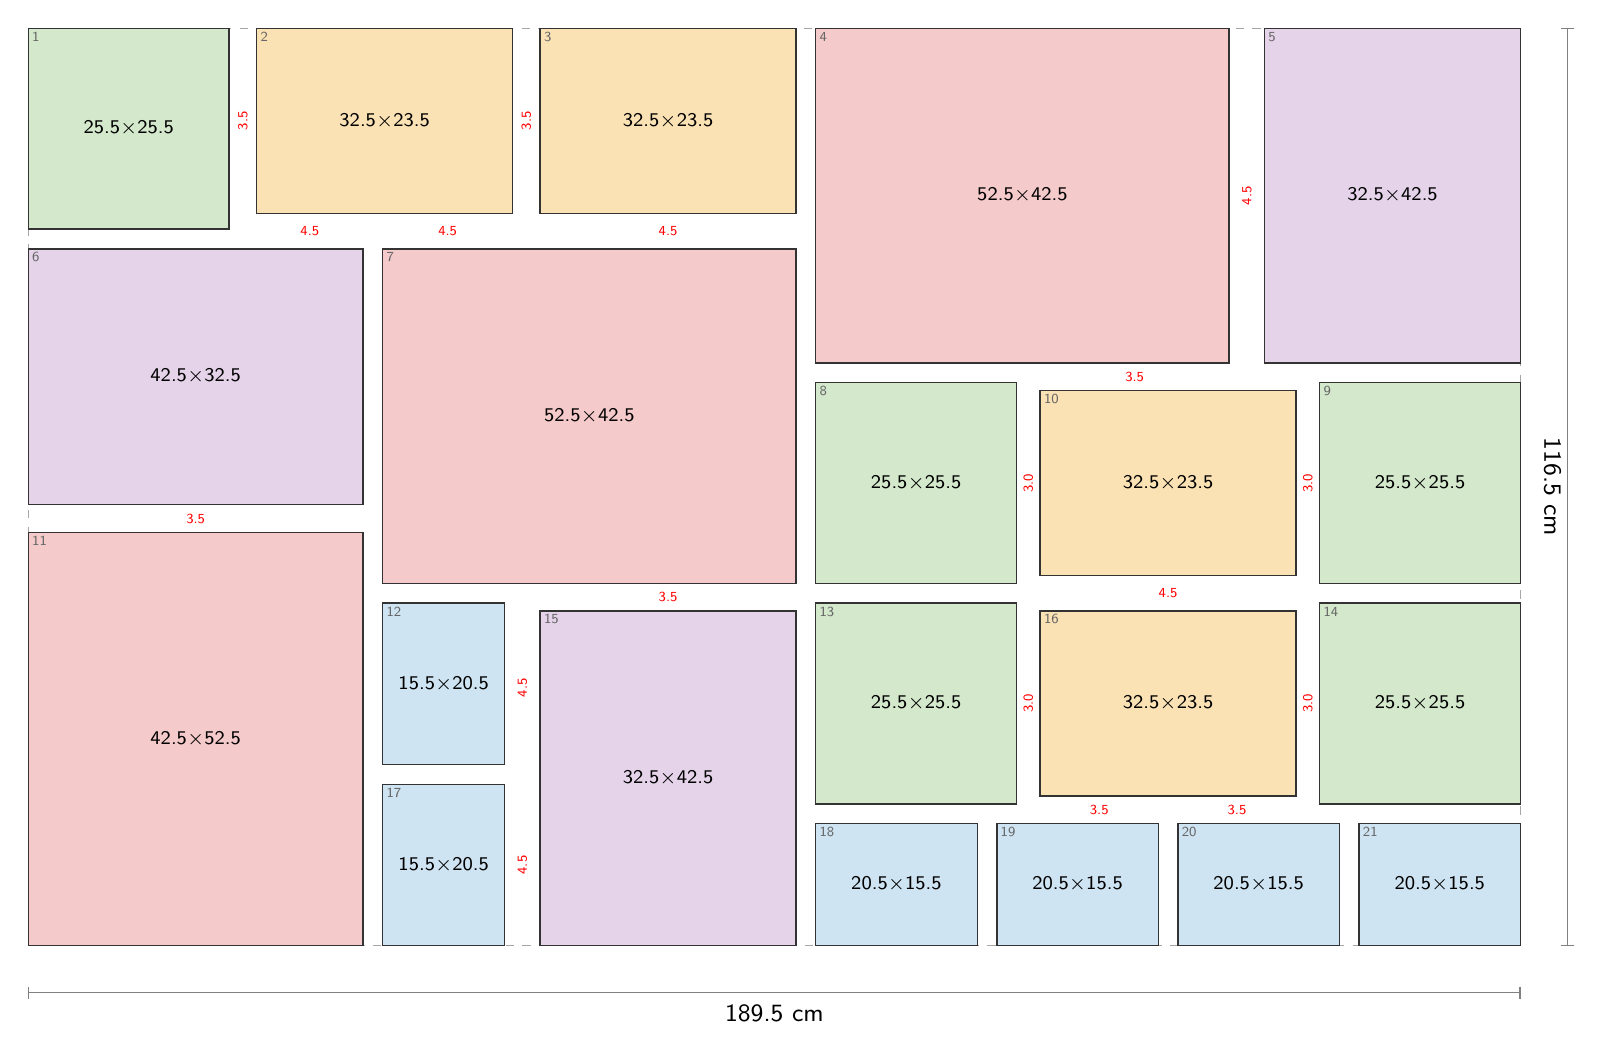
\begin{tikzpicture}[x=1mm, y=-1mm]
\draw[gray!70, dashed, line width=0.4pt] (0,0) rectangle (189.50,116.50);
\filldraw[fill=ft2, draw=black!80, line width=0.5pt] (0.00,0.00) rectangle (25.50,25.50);
\node[align=center, inner sep=0pt] at (12.75,12.75) {\scriptsize 25.5$\times$25.5};
\node[anchor=north west, inner sep=1.2pt, font=\tiny, text=black!60] at (0.00,0.00) {1};
\filldraw[fill=ft1, draw=black!80, line width=0.5pt] (29.00,0.00) rectangle (61.50,23.50);
\node[align=center, inner sep=0pt] at (45.25,11.75) {\scriptsize 32.5$\times$23.5};
\node[anchor=north west, inner sep=1.2pt, font=\tiny, text=black!60] at (29.00,0.00) {2};
\filldraw[fill=ft1, draw=black!80, line width=0.5pt] (65.00,0.00) rectangle (97.50,23.50);
\node[align=center, inner sep=0pt] at (81.25,11.75) {\scriptsize 32.5$\times$23.5};
\node[anchor=north west, inner sep=1.2pt, font=\tiny, text=black!60] at (65.00,0.00) {3};
\filldraw[fill=ft4, draw=black!80, line width=0.5pt] (100.00,0.00) rectangle (152.50,42.50);
\node[align=center, inner sep=0pt] at (126.25,21.25) {\scriptsize 52.5$\times$42.5};
\node[anchor=north west, inner sep=1.2pt, font=\tiny, text=black!60] at (100.00,0.00) {4};
\filldraw[fill=ft3, draw=black!80, line width=0.5pt] (157.00,0.00) rectangle (189.50,42.50);
\node[align=center, inner sep=0pt] at (173.25,21.25) {\scriptsize 32.5$\times$42.5};
\node[anchor=north west, inner sep=1.2pt, font=\tiny, text=black!60] at (157.00,0.00) {5};
\filldraw[fill=ft3, draw=black!80, line width=0.5pt] (0.00,28.00) rectangle (42.50,60.50);
\node[align=center, inner sep=0pt] at (21.25,44.25) {\scriptsize 42.5$\times$32.5};
\node[anchor=north west, inner sep=1.2pt, font=\tiny, text=black!60] at (0.00,28.00) {6};
\filldraw[fill=ft4, draw=black!80, line width=0.5pt] (45.00,28.00) rectangle (97.50,70.50);
\node[align=center, inner sep=0pt] at (71.25,49.25) {\scriptsize 52.5$\times$42.5};
\node[anchor=north west, inner sep=1.2pt, font=\tiny, text=black!60] at (45.00,28.00) {7};
\filldraw[fill=ft2, draw=black!80, line width=0.5pt] (100.00,45.00) rectangle (125.50,70.50);
\node[align=center, inner sep=0pt] at (112.75,57.75) {\scriptsize 25.5$\times$25.5};
\node[anchor=north west, inner sep=1.2pt, font=\tiny, text=black!60] at (100.00,45.00) {8};
\filldraw[fill=ft2, draw=black!80, line width=0.5pt] (164.00,45.00) rectangle (189.50,70.50);
\node[align=center, inner sep=0pt] at (176.75,57.75) {\scriptsize 25.5$\times$25.5};
\node[anchor=north west, inner sep=1.2pt, font=\tiny, text=black!60] at (164.00,45.00) {9};
\filldraw[fill=ft1, draw=black!80, line width=0.5pt] (128.50,46.00) rectangle (161.00,69.50);
\node[align=center, inner sep=0pt] at (144.75,57.75) {\scriptsize 32.5$\times$23.5};
\node[anchor=north west, inner sep=1.2pt, font=\tiny, text=black!60] at (128.50,46.00) {10};
\filldraw[fill=ft4, draw=black!80, line width=0.5pt] (0.00,64.00) rectangle (42.50,116.50);
\node[align=center, inner sep=0pt] at (21.25,90.25) {\scriptsize 42.5$\times$52.5};
\node[anchor=north west, inner sep=1.2pt, font=\tiny, text=black!60] at (0.00,64.00) {11};
\filldraw[fill=ft0, draw=black!80, line width=0.5pt] (45.00,73.00) rectangle (60.50,93.50);
\node[align=center, inner sep=0pt] at (52.75,83.25) {\scriptsize 15.5$\times$20.5};
\node[anchor=north west, inner sep=1.2pt, font=\tiny, text=black!60] at (45.00,73.00) {12};
\filldraw[fill=ft2, draw=black!80, line width=0.5pt] (100.00,73.00) rectangle (125.50,98.50);
\node[align=center, inner sep=0pt] at (112.75,85.75) {\scriptsize 25.5$\times$25.5};
\node[anchor=north west, inner sep=1.2pt, font=\tiny, text=black!60] at (100.00,73.00) {13};
\filldraw[fill=ft2, draw=black!80, line width=0.5pt] (164.00,73.00) rectangle (189.50,98.50);
\node[align=center, inner sep=0pt] at (176.75,85.75) {\scriptsize 25.5$\times$25.5};
\node[anchor=north west, inner sep=1.2pt, font=\tiny, text=black!60] at (164.00,73.00) {14};
\filldraw[fill=ft3, draw=black!80, line width=0.5pt] (65.00,74.00) rectangle (97.50,116.50);
\node[align=center, inner sep=0pt] at (81.25,95.25) {\scriptsize 32.5$\times$42.5};
\node[anchor=north west, inner sep=1.2pt, font=\tiny, text=black!60] at (65.00,74.00) {15};
\filldraw[fill=ft1, draw=black!80, line width=0.5pt] (128.50,74.00) rectangle (161.00,97.50);
\node[align=center, inner sep=0pt] at (144.75,85.75) {\scriptsize 32.5$\times$23.5};
\node[anchor=north west, inner sep=1.2pt, font=\tiny, text=black!60] at (128.50,74.00) {16};
\filldraw[fill=ft0, draw=black!80, line width=0.5pt] (45.00,96.00) rectangle (60.50,116.50);
\node[align=center, inner sep=0pt] at (52.75,106.25) {\scriptsize 15.5$\times$20.5};
\node[anchor=north west, inner sep=1.2pt, font=\tiny, text=black!60] at (45.00,96.00) {17};
\filldraw[fill=ft0, draw=black!80, line width=0.5pt] (100.00,101.00) rectangle (120.50,116.50);
\node[align=center, inner sep=0pt] at (110.25,108.75) {\scriptsize 20.5$\times$15.5};
\node[anchor=north west, inner sep=1.2pt, font=\tiny, text=black!60] at (100.00,101.00) {18};
\filldraw[fill=ft0, draw=black!80, line width=0.5pt] (123.00,101.00) rectangle (143.50,116.50);
\node[align=center, inner sep=0pt] at (133.25,108.75) {\scriptsize 20.5$\times$15.5};
\node[anchor=north west, inner sep=1.2pt, font=\tiny, text=black!60] at (123.00,101.00) {19};
\filldraw[fill=ft0, draw=black!80, line width=0.5pt] (146.00,101.00) rectangle (166.50,116.50);
\node[align=center, inner sep=0pt] at (156.25,108.75) {\scriptsize 20.5$\times$15.5};
\node[anchor=north west, inner sep=1.2pt, font=\tiny, text=black!60] at (146.00,101.00) {20};
\filldraw[fill=ft0, draw=black!80, line width=0.5pt] (169.00,101.00) rectangle (189.50,116.50);
\node[align=center, inner sep=0pt] at (179.25,108.75) {\scriptsize 20.5$\times$15.5};
\node[anchor=north west, inner sep=1.2pt, font=\tiny, text=black!60] at (169.00,101.00) {21};
\node[font=\tiny, text=red, fill=white, inner sep=0.3pt, rotate=90] at (27.25,11.75) {3.5};
\node[font=\tiny, text=red, fill=white, inner sep=0.3pt, rotate=90] at (63.25,11.75) {3.5};
\node[font=\tiny, text=red, fill=white, inner sep=0.3pt] at (35.75,25.75) {4.5};
\node[font=\tiny, text=red, fill=white, inner sep=0.3pt] at (53.25,25.75) {4.5};
\node[font=\tiny, text=red, fill=white, inner sep=0.3pt] at (81.25,25.75) {4.5};
\node[font=\tiny, text=red, fill=white, inner sep=0.3pt, rotate=90] at (154.75,21.25) {4.5};
\node[font=\tiny, text=red, fill=white, inner sep=0.3pt] at (140.50,44.25) {3.5};
\node[font=\tiny, text=red, fill=white, inner sep=0.3pt] at (21.25,62.25) {3.5};
\node[font=\tiny, text=red, fill=white, inner sep=0.3pt] at (81.25,72.25) {3.5};
\node[font=\tiny, text=red, fill=white, inner sep=0.3pt, rotate=90] at (127.00,57.75) {3.0};
\node[font=\tiny, text=red, fill=white, inner sep=0.3pt, rotate=90] at (162.50,57.75) {3.0};
\node[font=\tiny, text=red, fill=white, inner sep=0.3pt] at (144.75,71.75) {4.5};
\node[font=\tiny, text=red, fill=white, inner sep=0.3pt, rotate=90] at (62.75,83.75) {4.5};
\node[font=\tiny, text=red, fill=white, inner sep=0.3pt, rotate=90] at (127.00,85.75) {3.0};
\node[font=\tiny, text=red, fill=white, inner sep=0.3pt, rotate=90] at (162.50,85.75) {3.0};
\node[font=\tiny, text=red, fill=white, inner sep=0.3pt] at (136.00,99.25) {3.5};
\node[font=\tiny, text=red, fill=white, inner sep=0.3pt] at (153.50,99.25) {3.5};
\node[font=\tiny, text=red, fill=white, inner sep=0.3pt, rotate=90] at (62.75,106.25) {4.5};
\draw[Bar-Bar, gray] (0,122.50) -- (189.50,122.50) node[midway, below=1pt, font=\small, text=black] {189.5 cm};
\draw[Bar-Bar, gray] (195.50,0) -- (195.50,116.50) node[midway, right=1pt, font=\small, text=black, rotate=-90, anchor=north] {116.5 cm};
\end{tikzpicture}\\[4pt]
{\scriptsize Scale 1:10 (1 mm = 1 cm). Red numbers mark gaps that deviate from the nominal gap by more than 0.25 cm. Small grey numbers index the coordinate table.}
\end{minipage}\hfill
\begin{minipage}[t]{0.25\textwidth}\vspace{0pt}
\small
\begin{tabular}{@{}l l@{}}
\toprule
Outer size & 189.5 $\times$ 116.5 cm \\
Nominal gap & 2.5 cm \\
Actual gaps & 2.5 -- 4.5 cm \\
Max.\ deviation & 2.0 cm \\
Mean deviation & 0.59 cm \\
Border notches & top 4 cm, bottom 4 cm \\
Corners filled & 4 / 4 \\
Frames used & 21 of 28 \\
Large frames & {\scriptsize 3, touching 2$\times$ (21 cm), min.\ dist.\ 62 cm} \\
Entropy & 0.78 \\
\quad {\scriptsize mix / variety} & {\scriptsize 0.88 / 0.75} \\
\quad {\scriptsize stagger / lines} & {\scriptsize 0.50 / 1.00 (1 through)} \\
\bottomrule
\end{tabular}

\vspace{8pt}
\scriptsize
\begin{tabular}{@{}c l l r r@{}}
\toprule
 & outer w $\times$ h (cm) &  & used & have \\
\midrule
\tikz[baseline=-0.6ex]\fill[ft0,draw=black!60] (0,0) rectangle (1.2ex,1.2ex); & 20.5$\times$15.5 & L & 4 & 9 \\
\tikz[baseline=-0.6ex]\fill[ft0,draw=black!60] (0,0) rectangle (1.2ex,1.2ex); & 15.5$\times$20.5 & P & 2 & 2 \\
\tikz[baseline=-0.6ex]\fill[ft3,draw=black!60] (0,0) rectangle (1.2ex,1.2ex); & 32.5$\times$42.5 & P & 2 & 2 \\
\tikz[baseline=-0.6ex]\fill[ft3,draw=black!60] (0,0) rectangle (1.2ex,1.2ex); & 42.5$\times$32.5 & L & 1 & 1 \\
\tikz[baseline=-0.6ex]\fill[ft1,draw=black!60] (0,0) rectangle (1.2ex,1.2ex); & 32.5$\times$23.5 & L & 4 & 5 \\
\tikz[baseline=-0.6ex]\fill[ft1,draw=black!60] (0,0) rectangle (1.2ex,1.2ex); & 23.5$\times$32.5 & P & 0 & 1 \\
\tikz[baseline=-0.6ex]\fill[ft2,draw=black!60] (0,0) rectangle (1.2ex,1.2ex); & 25.5$\times$25.5 &  & 5 & 5 \\
\tikz[baseline=-0.6ex]\fill[ft4,draw=black!60] (0,0) rectangle (1.2ex,1.2ex); & 42.5$\times$52.5 & P & 1 & 1 \\
\tikz[baseline=-0.6ex]\fill[ft4,draw=black!60] (0,0) rectangle (1.2ex,1.2ex); & 52.5$\times$42.5 & L & 2 & 2 \\
\bottomrule
\end{tabular}

\vspace{8pt}
{\bfseries Positions} (top-left corner, cm)\\[2pt]
\tiny
\begin{tabular}{@{}r l r r@{}}
\toprule
\# & frame w $\times$ h & x & y \\
\midrule
1 & 25.5 $\times$ 25.5 & 0.0 & 0.0 \\
2 & 32.5 $\times$ 23.5 & 29.0 & 0.0 \\
3 & 32.5 $\times$ 23.5 & 65.0 & 0.0 \\
4 & 52.5 $\times$ 42.5 & 100.0 & 0.0 \\
5 & 32.5 $\times$ 42.5 & 157.0 & 0.0 \\
6 & 42.5 $\times$ 32.5 & 0.0 & 28.0 \\
7 & 52.5 $\times$ 42.5 & 45.0 & 28.0 \\
8 & 25.5 $\times$ 25.5 & 100.0 & 45.0 \\
9 & 25.5 $\times$ 25.5 & 164.0 & 45.0 \\
10 & 32.5 $\times$ 23.5 & 128.5 & 46.0 \\
11 & 42.5 $\times$ 52.5 & 0.0 & 64.0 \\
12 & 15.5 $\times$ 20.5 & 45.0 & 73.0 \\
13 & 25.5 $\times$ 25.5 & 100.0 & 73.0 \\
14 & 25.5 $\times$ 25.5 & 164.0 & 73.0 \\
15 & 32.5 $\times$ 42.5 & 65.0 & 74.0 \\
16 & 32.5 $\times$ 23.5 & 128.5 & 74.0 \\
17 & 15.5 $\times$ 20.5 & 45.0 & 96.0 \\
18 & 20.5 $\times$ 15.5 & 100.0 & 101.0 \\
19 & 20.5 $\times$ 15.5 & 123.0 & 101.0 \\
20 & 20.5 $\times$ 15.5 & 146.0 & 101.0 \\
21 & 20.5 $\times$ 15.5 & 169.0 & 101.0 \\
\bottomrule
\end{tabular}
\end{minipage}
\clearpage

\phantomsection\addcontentsline{toc}{subsection}{Layout 12: 177.5 \texorpdfstring{$\times$}{x} 113.5 cm, 21 frames, gap 1.5 cm, max.\ deviation 2.0 cm}
\label{lay:per-run-gap:12}
\begin{minipage}[t]{0.74\textwidth}\vspace{0pt}
{\LARGE\bfseries Layout 12}\hspace{1.5em}{\large 177.5 $\times$ 113.5 cm \quad gap 1.5 cm \quad 21 frames}\\[8pt]
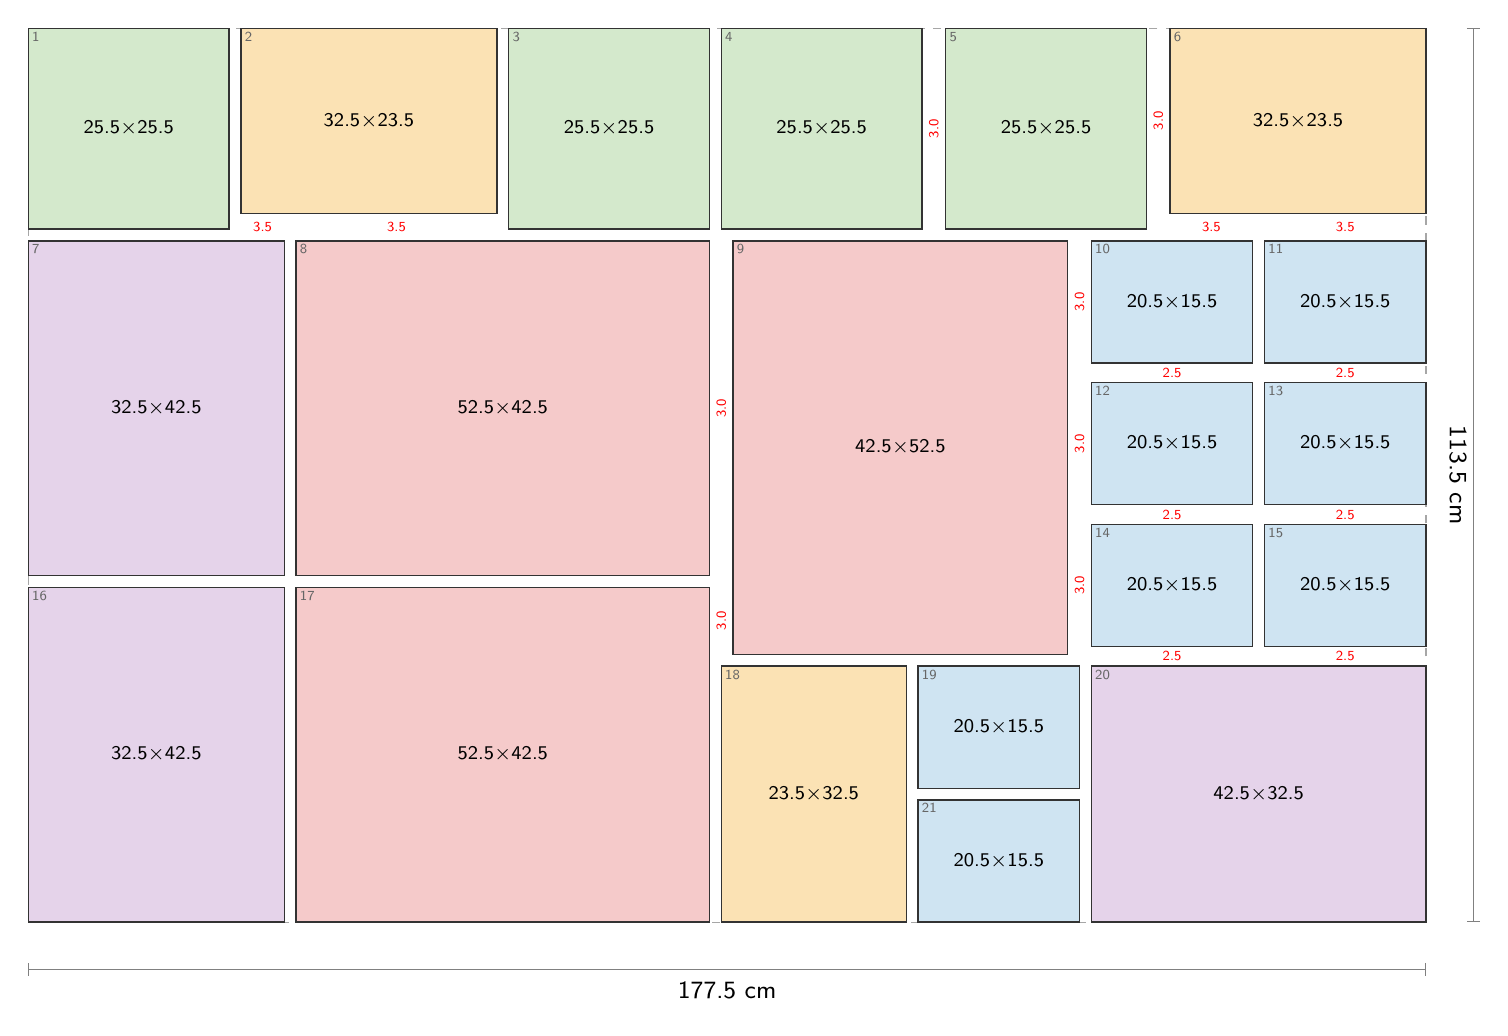
\begin{tikzpicture}[x=1mm, y=-1mm]
\draw[gray!70, dashed, line width=0.4pt] (0,0) rectangle (177.50,113.50);
\filldraw[fill=ft2, draw=black!80, line width=0.5pt] (0.00,0.00) rectangle (25.50,25.50);
\node[align=center, inner sep=0pt] at (12.75,12.75) {\scriptsize 25.5$\times$25.5};
\node[anchor=north west, inner sep=1.2pt, font=\tiny, text=black!60] at (0.00,0.00) {1};
\filldraw[fill=ft1, draw=black!80, line width=0.5pt] (27.00,0.00) rectangle (59.50,23.50);
\node[align=center, inner sep=0pt] at (43.25,11.75) {\scriptsize 32.5$\times$23.5};
\node[anchor=north west, inner sep=1.2pt, font=\tiny, text=black!60] at (27.00,0.00) {2};
\filldraw[fill=ft2, draw=black!80, line width=0.5pt] (61.00,0.00) rectangle (86.50,25.50);
\node[align=center, inner sep=0pt] at (73.75,12.75) {\scriptsize 25.5$\times$25.5};
\node[anchor=north west, inner sep=1.2pt, font=\tiny, text=black!60] at (61.00,0.00) {3};
\filldraw[fill=ft2, draw=black!80, line width=0.5pt] (88.00,0.00) rectangle (113.50,25.50);
\node[align=center, inner sep=0pt] at (100.75,12.75) {\scriptsize 25.5$\times$25.5};
\node[anchor=north west, inner sep=1.2pt, font=\tiny, text=black!60] at (88.00,0.00) {4};
\filldraw[fill=ft2, draw=black!80, line width=0.5pt] (116.50,0.00) rectangle (142.00,25.50);
\node[align=center, inner sep=0pt] at (129.25,12.75) {\scriptsize 25.5$\times$25.5};
\node[anchor=north west, inner sep=1.2pt, font=\tiny, text=black!60] at (116.50,0.00) {5};
\filldraw[fill=ft1, draw=black!80, line width=0.5pt] (145.00,0.00) rectangle (177.50,23.50);
\node[align=center, inner sep=0pt] at (161.25,11.75) {\scriptsize 32.5$\times$23.5};
\node[anchor=north west, inner sep=1.2pt, font=\tiny, text=black!60] at (145.00,0.00) {6};
\filldraw[fill=ft3, draw=black!80, line width=0.5pt] (0.00,27.00) rectangle (32.50,69.50);
\node[align=center, inner sep=0pt] at (16.25,48.25) {\scriptsize 32.5$\times$42.5};
\node[anchor=north west, inner sep=1.2pt, font=\tiny, text=black!60] at (0.00,27.00) {7};
\filldraw[fill=ft4, draw=black!80, line width=0.5pt] (34.00,27.00) rectangle (86.50,69.50);
\node[align=center, inner sep=0pt] at (60.25,48.25) {\scriptsize 52.5$\times$42.5};
\node[anchor=north west, inner sep=1.2pt, font=\tiny, text=black!60] at (34.00,27.00) {8};
\filldraw[fill=ft4, draw=black!80, line width=0.5pt] (89.50,27.00) rectangle (132.00,79.50);
\node[align=center, inner sep=0pt] at (110.75,53.25) {\scriptsize 42.5$\times$52.5};
\node[anchor=north west, inner sep=1.2pt, font=\tiny, text=black!60] at (89.50,27.00) {9};
\filldraw[fill=ft0, draw=black!80, line width=0.5pt] (135.00,27.00) rectangle (155.50,42.50);
\node[align=center, inner sep=0pt] at (145.25,34.75) {\scriptsize 20.5$\times$15.5};
\node[anchor=north west, inner sep=1.2pt, font=\tiny, text=black!60] at (135.00,27.00) {10};
\filldraw[fill=ft0, draw=black!80, line width=0.5pt] (157.00,27.00) rectangle (177.50,42.50);
\node[align=center, inner sep=0pt] at (167.25,34.75) {\scriptsize 20.5$\times$15.5};
\node[anchor=north west, inner sep=1.2pt, font=\tiny, text=black!60] at (157.00,27.00) {11};
\filldraw[fill=ft0, draw=black!80, line width=0.5pt] (135.00,45.00) rectangle (155.50,60.50);
\node[align=center, inner sep=0pt] at (145.25,52.75) {\scriptsize 20.5$\times$15.5};
\node[anchor=north west, inner sep=1.2pt, font=\tiny, text=black!60] at (135.00,45.00) {12};
\filldraw[fill=ft0, draw=black!80, line width=0.5pt] (157.00,45.00) rectangle (177.50,60.50);
\node[align=center, inner sep=0pt] at (167.25,52.75) {\scriptsize 20.5$\times$15.5};
\node[anchor=north west, inner sep=1.2pt, font=\tiny, text=black!60] at (157.00,45.00) {13};
\filldraw[fill=ft0, draw=black!80, line width=0.5pt] (135.00,63.00) rectangle (155.50,78.50);
\node[align=center, inner sep=0pt] at (145.25,70.75) {\scriptsize 20.5$\times$15.5};
\node[anchor=north west, inner sep=1.2pt, font=\tiny, text=black!60] at (135.00,63.00) {14};
\filldraw[fill=ft0, draw=black!80, line width=0.5pt] (157.00,63.00) rectangle (177.50,78.50);
\node[align=center, inner sep=0pt] at (167.25,70.75) {\scriptsize 20.5$\times$15.5};
\node[anchor=north west, inner sep=1.2pt, font=\tiny, text=black!60] at (157.00,63.00) {15};
\filldraw[fill=ft3, draw=black!80, line width=0.5pt] (0.00,71.00) rectangle (32.50,113.50);
\node[align=center, inner sep=0pt] at (16.25,92.25) {\scriptsize 32.5$\times$42.5};
\node[anchor=north west, inner sep=1.2pt, font=\tiny, text=black!60] at (0.00,71.00) {16};
\filldraw[fill=ft4, draw=black!80, line width=0.5pt] (34.00,71.00) rectangle (86.50,113.50);
\node[align=center, inner sep=0pt] at (60.25,92.25) {\scriptsize 52.5$\times$42.5};
\node[anchor=north west, inner sep=1.2pt, font=\tiny, text=black!60] at (34.00,71.00) {17};
\filldraw[fill=ft1, draw=black!80, line width=0.5pt] (88.00,81.00) rectangle (111.50,113.50);
\node[align=center, inner sep=0pt] at (99.75,97.25) {\scriptsize 23.5$\times$32.5};
\node[anchor=north west, inner sep=1.2pt, font=\tiny, text=black!60] at (88.00,81.00) {18};
\filldraw[fill=ft0, draw=black!80, line width=0.5pt] (113.00,81.00) rectangle (133.50,96.50);
\node[align=center, inner sep=0pt] at (123.25,88.75) {\scriptsize 20.5$\times$15.5};
\node[anchor=north west, inner sep=1.2pt, font=\tiny, text=black!60] at (113.00,81.00) {19};
\filldraw[fill=ft3, draw=black!80, line width=0.5pt] (135.00,81.00) rectangle (177.50,113.50);
\node[align=center, inner sep=0pt] at (156.25,97.25) {\scriptsize 42.5$\times$32.5};
\node[anchor=north west, inner sep=1.2pt, font=\tiny, text=black!60] at (135.00,81.00) {20};
\filldraw[fill=ft0, draw=black!80, line width=0.5pt] (113.00,98.00) rectangle (133.50,113.50);
\node[align=center, inner sep=0pt] at (123.25,105.75) {\scriptsize 20.5$\times$15.5};
\node[anchor=north west, inner sep=1.2pt, font=\tiny, text=black!60] at (113.00,98.00) {21};
\node[font=\tiny, text=red, fill=white, inner sep=0.3pt] at (29.75,25.25) {3.5};
\node[font=\tiny, text=red, fill=white, inner sep=0.3pt] at (46.75,25.25) {3.5};
\node[font=\tiny, text=red, fill=white, inner sep=0.3pt, rotate=90] at (115.00,12.75) {3.0};
\node[font=\tiny, text=red, fill=white, inner sep=0.3pt, rotate=90] at (143.50,11.75) {3.0};
\node[font=\tiny, text=red, fill=white, inner sep=0.3pt] at (150.25,25.25) {3.5};
\node[font=\tiny, text=red, fill=white, inner sep=0.3pt] at (167.25,25.25) {3.5};
\node[font=\tiny, text=red, fill=white, inner sep=0.3pt, rotate=90] at (88.00,48.25) {3.0};
\node[font=\tiny, text=red, fill=white, inner sep=0.3pt, rotate=90] at (133.50,34.75) {3.0};
\node[font=\tiny, text=red, fill=white, inner sep=0.3pt, rotate=90] at (133.50,52.75) {3.0};
\node[font=\tiny, text=red, fill=white, inner sep=0.3pt, rotate=90] at (133.50,70.75) {3.0};
\node[font=\tiny, text=red, fill=white, inner sep=0.3pt] at (145.25,43.75) {2.5};
\node[font=\tiny, text=red, fill=white, inner sep=0.3pt] at (167.25,43.75) {2.5};
\node[font=\tiny, text=red, fill=white, inner sep=0.3pt] at (145.25,61.75) {2.5};
\node[font=\tiny, text=red, fill=white, inner sep=0.3pt] at (167.25,61.75) {2.5};
\node[font=\tiny, text=red, fill=white, inner sep=0.3pt] at (145.25,79.75) {2.5};
\node[font=\tiny, text=red, fill=white, inner sep=0.3pt] at (167.25,79.75) {2.5};
\node[font=\tiny, text=red, fill=white, inner sep=0.3pt, rotate=90] at (88.00,75.25) {3.0};
\draw[Bar-Bar, gray] (0,119.50) -- (177.50,119.50) node[midway, below=1pt, font=\small, text=black] {177.5 cm};
\draw[Bar-Bar, gray] (183.50,0) -- (183.50,113.50) node[midway, right=1pt, font=\small, text=black, rotate=-90, anchor=north] {113.5 cm};
\end{tikzpicture}\\[4pt]
{\scriptsize Scale 1:10 (1 mm = 1 cm). Red numbers mark gaps that deviate from the nominal gap by more than 0.25 cm. Small grey numbers index the coordinate table.}
\end{minipage}\hfill
\begin{minipage}[t]{0.25\textwidth}\vspace{0pt}
\small
\begin{tabular}{@{}l l@{}}
\toprule
Outer size & 177.5 $\times$ 113.5 cm \\
Nominal gap & 1.5 cm \\
Actual gaps & 1.5 -- 3.5 cm \\
Max.\ deviation & 2.0 cm \\
Mean deviation & 0.61 cm \\
Border notches & top 6 cm, right 4 cm \\
Corners filled & 4 / 4 \\
Frames used & 21 of 28 \\
Large frames & {\scriptsize 3, touching 1$\times$ (52 cm), min.\ dist.\ 44 cm} \\
Entropy & 0.66 \\
\quad {\scriptsize mix / variety} & {\scriptsize 0.81 / 0.62} \\
\quad {\scriptsize stagger / lines} & {\scriptsize 0.45 / 0.75 (2 through)} \\
\bottomrule
\end{tabular}

\vspace{8pt}
\scriptsize
\begin{tabular}{@{}c l l r r@{}}
\toprule
 & outer w $\times$ h (cm) &  & used & have \\
\midrule
\tikz[baseline=-0.6ex]\fill[ft0,draw=black!60] (0,0) rectangle (1.2ex,1.2ex); & 20.5$\times$15.5 & L & 8 & 9 \\
\tikz[baseline=-0.6ex]\fill[ft0,draw=black!60] (0,0) rectangle (1.2ex,1.2ex); & 15.5$\times$20.5 & P & 0 & 2 \\
\tikz[baseline=-0.6ex]\fill[ft3,draw=black!60] (0,0) rectangle (1.2ex,1.2ex); & 32.5$\times$42.5 & P & 2 & 2 \\
\tikz[baseline=-0.6ex]\fill[ft3,draw=black!60] (0,0) rectangle (1.2ex,1.2ex); & 42.5$\times$32.5 & L & 1 & 1 \\
\tikz[baseline=-0.6ex]\fill[ft1,draw=black!60] (0,0) rectangle (1.2ex,1.2ex); & 32.5$\times$23.5 & L & 2 & 5 \\
\tikz[baseline=-0.6ex]\fill[ft1,draw=black!60] (0,0) rectangle (1.2ex,1.2ex); & 23.5$\times$32.5 & P & 1 & 1 \\
\tikz[baseline=-0.6ex]\fill[ft2,draw=black!60] (0,0) rectangle (1.2ex,1.2ex); & 25.5$\times$25.5 &  & 4 & 5 \\
\tikz[baseline=-0.6ex]\fill[ft4,draw=black!60] (0,0) rectangle (1.2ex,1.2ex); & 42.5$\times$52.5 & P & 1 & 1 \\
\tikz[baseline=-0.6ex]\fill[ft4,draw=black!60] (0,0) rectangle (1.2ex,1.2ex); & 52.5$\times$42.5 & L & 2 & 2 \\
\bottomrule
\end{tabular}

\vspace{8pt}
{\bfseries Positions} (top-left corner, cm)\\[2pt]
\tiny
\begin{tabular}{@{}r l r r@{}}
\toprule
\# & frame w $\times$ h & x & y \\
\midrule
1 & 25.5 $\times$ 25.5 & 0.0 & 0.0 \\
2 & 32.5 $\times$ 23.5 & 27.0 & 0.0 \\
3 & 25.5 $\times$ 25.5 & 61.0 & 0.0 \\
4 & 25.5 $\times$ 25.5 & 88.0 & 0.0 \\
5 & 25.5 $\times$ 25.5 & 116.5 & 0.0 \\
6 & 32.5 $\times$ 23.5 & 145.0 & 0.0 \\
7 & 32.5 $\times$ 42.5 & 0.0 & 27.0 \\
8 & 52.5 $\times$ 42.5 & 34.0 & 27.0 \\
9 & 42.5 $\times$ 52.5 & 89.5 & 27.0 \\
10 & 20.5 $\times$ 15.5 & 135.0 & 27.0 \\
11 & 20.5 $\times$ 15.5 & 157.0 & 27.0 \\
12 & 20.5 $\times$ 15.5 & 135.0 & 45.0 \\
13 & 20.5 $\times$ 15.5 & 157.0 & 45.0 \\
14 & 20.5 $\times$ 15.5 & 135.0 & 63.0 \\
15 & 20.5 $\times$ 15.5 & 157.0 & 63.0 \\
16 & 32.5 $\times$ 42.5 & 0.0 & 71.0 \\
17 & 52.5 $\times$ 42.5 & 34.0 & 71.0 \\
18 & 23.5 $\times$ 32.5 & 88.0 & 81.0 \\
19 & 20.5 $\times$ 15.5 & 113.0 & 81.0 \\
20 & 42.5 $\times$ 32.5 & 135.0 & 81.0 \\
21 & 20.5 $\times$ 15.5 & 113.0 & 98.0 \\
\bottomrule
\end{tabular}
\end{minipage}
\clearpage

\phantomsection\addcontentsline{toc}{subsection}{Layout 13: 179.5 \texorpdfstring{$\times$}{x} 126.5 cm, 21 frames, gap 5.5 cm, max.\ deviation 2.7 cm}
\label{lay:per-run-gap:13}
\begin{minipage}[t]{0.74\textwidth}\vspace{0pt}
{\LARGE\bfseries Layout 13}\hspace{1.5em}{\large 179.5 $\times$ 126.5 cm \quad gap 5.5 cm \quad 21 frames}\\[8pt]
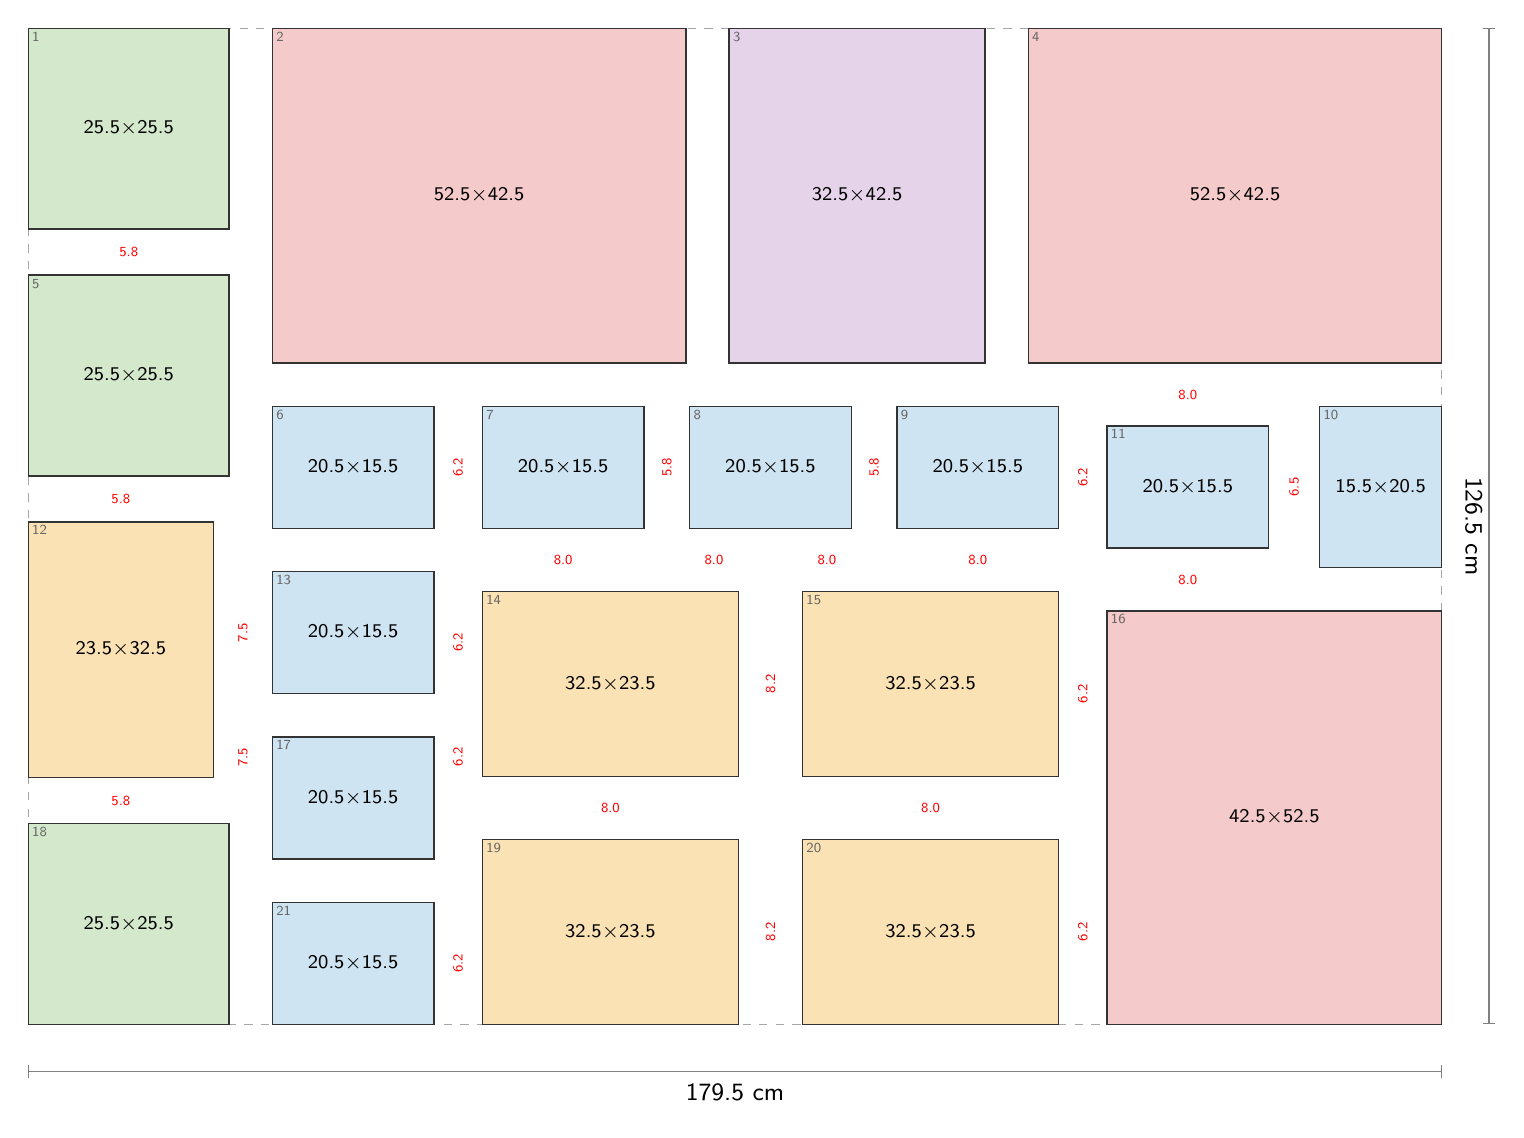
\begin{tikzpicture}[x=1mm, y=-1mm]
\draw[gray!70, dashed, line width=0.4pt] (0,0) rectangle (179.50,126.50);
\filldraw[fill=ft2, draw=black!80, line width=0.5pt] (0.00,0.00) rectangle (25.50,25.50);
\node[align=center, inner sep=0pt] at (12.75,12.75) {\scriptsize 25.5$\times$25.5};
\node[anchor=north west, inner sep=1.2pt, font=\tiny, text=black!60] at (0.00,0.00) {1};
\filldraw[fill=ft4, draw=black!80, line width=0.5pt] (31.00,0.00) rectangle (83.50,42.50);
\node[align=center, inner sep=0pt] at (57.25,21.25) {\scriptsize 52.5$\times$42.5};
\node[anchor=north west, inner sep=1.2pt, font=\tiny, text=black!60] at (31.00,0.00) {2};
\filldraw[fill=ft3, draw=black!80, line width=0.5pt] (89.00,0.00) rectangle (121.50,42.50);
\node[align=center, inner sep=0pt] at (105.25,21.25) {\scriptsize 32.5$\times$42.5};
\node[anchor=north west, inner sep=1.2pt, font=\tiny, text=black!60] at (89.00,0.00) {3};
\filldraw[fill=ft4, draw=black!80, line width=0.5pt] (127.00,0.00) rectangle (179.50,42.50);
\node[align=center, inner sep=0pt] at (153.25,21.25) {\scriptsize 52.5$\times$42.5};
\node[anchor=north west, inner sep=1.2pt, font=\tiny, text=black!60] at (127.00,0.00) {4};
\filldraw[fill=ft2, draw=black!80, line width=0.5pt] (0.00,31.33) rectangle (25.50,56.83);
\node[align=center, inner sep=0pt] at (12.75,44.08) {\scriptsize 25.5$\times$25.5};
\node[anchor=north west, inner sep=1.2pt, font=\tiny, text=black!60] at (0.00,31.33) {5};
\filldraw[fill=ft0, draw=black!80, line width=0.5pt] (31.00,48.00) rectangle (51.50,63.50);
\node[align=center, inner sep=0pt] at (41.25,55.75) {\scriptsize 20.5$\times$15.5};
\node[anchor=north west, inner sep=1.2pt, font=\tiny, text=black!60] at (31.00,48.00) {6};
\filldraw[fill=ft0, draw=black!80, line width=0.5pt] (57.67,48.00) rectangle (78.17,63.50);
\node[align=center, inner sep=0pt] at (67.92,55.75) {\scriptsize 20.5$\times$15.5};
\node[anchor=north west, inner sep=1.2pt, font=\tiny, text=black!60] at (57.67,48.00) {7};
\filldraw[fill=ft0, draw=black!80, line width=0.5pt] (84.00,48.00) rectangle (104.50,63.50);
\node[align=center, inner sep=0pt] at (94.25,55.75) {\scriptsize 20.5$\times$15.5};
\node[anchor=north west, inner sep=1.2pt, font=\tiny, text=black!60] at (84.00,48.00) {8};
\filldraw[fill=ft0, draw=black!80, line width=0.5pt] (110.33,48.00) rectangle (130.83,63.50);
\node[align=center, inner sep=0pt] at (120.58,55.75) {\scriptsize 20.5$\times$15.5};
\node[anchor=north west, inner sep=1.2pt, font=\tiny, text=black!60] at (110.33,48.00) {9};
\filldraw[fill=ft0, draw=black!80, line width=0.5pt] (164.00,48.00) rectangle (179.50,68.50);
\node[align=center, inner sep=0pt] at (171.75,58.25) {\scriptsize 15.5$\times$20.5};
\node[anchor=north west, inner sep=1.2pt, font=\tiny, text=black!60] at (164.00,48.00) {10};
\filldraw[fill=ft0, draw=black!80, line width=0.5pt] (137.00,50.50) rectangle (157.50,66.00);
\node[align=center, inner sep=0pt] at (147.25,58.25) {\scriptsize 20.5$\times$15.5};
\node[anchor=north west, inner sep=1.2pt, font=\tiny, text=black!60] at (137.00,50.50) {11};
\filldraw[fill=ft1, draw=black!80, line width=0.5pt] (0.00,62.67) rectangle (23.50,95.17);
\node[align=center, inner sep=0pt] at (11.75,78.92) {\scriptsize 23.5$\times$32.5};
\node[anchor=north west, inner sep=1.2pt, font=\tiny, text=black!60] at (0.00,62.67) {12};
\filldraw[fill=ft0, draw=black!80, line width=0.5pt] (31.00,69.00) rectangle (51.50,84.50);
\node[align=center, inner sep=0pt] at (41.25,76.75) {\scriptsize 20.5$\times$15.5};
\node[anchor=north west, inner sep=1.2pt, font=\tiny, text=black!60] at (31.00,69.00) {13};
\filldraw[fill=ft1, draw=black!80, line width=0.5pt] (57.67,71.50) rectangle (90.17,95.00);
\node[align=center, inner sep=0pt] at (73.92,83.25) {\scriptsize 32.5$\times$23.5};
\node[anchor=north west, inner sep=1.2pt, font=\tiny, text=black!60] at (57.67,71.50) {14};
\filldraw[fill=ft1, draw=black!80, line width=0.5pt] (98.33,71.50) rectangle (130.83,95.00);
\node[align=center, inner sep=0pt] at (114.58,83.25) {\scriptsize 32.5$\times$23.5};
\node[anchor=north west, inner sep=1.2pt, font=\tiny, text=black!60] at (98.33,71.50) {15};
\filldraw[fill=ft4, draw=black!80, line width=0.5pt] (137.00,74.00) rectangle (179.50,126.50);
\node[align=center, inner sep=0pt] at (158.25,100.25) {\scriptsize 42.5$\times$52.5};
\node[anchor=north west, inner sep=1.2pt, font=\tiny, text=black!60] at (137.00,74.00) {16};
\filldraw[fill=ft0, draw=black!80, line width=0.5pt] (31.00,90.00) rectangle (51.50,105.50);
\node[align=center, inner sep=0pt] at (41.25,97.75) {\scriptsize 20.5$\times$15.5};
\node[anchor=north west, inner sep=1.2pt, font=\tiny, text=black!60] at (31.00,90.00) {17};
\filldraw[fill=ft2, draw=black!80, line width=0.5pt] (0.00,101.00) rectangle (25.50,126.50);
\node[align=center, inner sep=0pt] at (12.75,113.75) {\scriptsize 25.5$\times$25.5};
\node[anchor=north west, inner sep=1.2pt, font=\tiny, text=black!60] at (0.00,101.00) {18};
\filldraw[fill=ft1, draw=black!80, line width=0.5pt] (57.67,103.00) rectangle (90.17,126.50);
\node[align=center, inner sep=0pt] at (73.92,114.75) {\scriptsize 32.5$\times$23.5};
\node[anchor=north west, inner sep=1.2pt, font=\tiny, text=black!60] at (57.67,103.00) {19};
\filldraw[fill=ft1, draw=black!80, line width=0.5pt] (98.33,103.00) rectangle (130.83,126.50);
\node[align=center, inner sep=0pt] at (114.58,114.75) {\scriptsize 32.5$\times$23.5};
\node[anchor=north west, inner sep=1.2pt, font=\tiny, text=black!60] at (98.33,103.00) {20};
\filldraw[fill=ft0, draw=black!80, line width=0.5pt] (31.00,111.00) rectangle (51.50,126.50);
\node[align=center, inner sep=0pt] at (41.25,118.75) {\scriptsize 20.5$\times$15.5};
\node[anchor=north west, inner sep=1.2pt, font=\tiny, text=black!60] at (31.00,111.00) {21};
\node[font=\tiny, text=red, fill=white, inner sep=0.3pt] at (12.75,28.42) {5.8};
\node[font=\tiny, text=red, fill=white, inner sep=0.3pt] at (147.25,46.50) {8.0};
\node[font=\tiny, text=red, fill=white, inner sep=0.3pt] at (11.75,59.75) {5.8};
\node[font=\tiny, text=red, fill=white, inner sep=0.3pt, rotate=90] at (54.58,55.75) {6.2};
\node[font=\tiny, text=red, fill=white, inner sep=0.3pt, rotate=90] at (81.08,55.75) {5.8};
\node[font=\tiny, text=red, fill=white, inner sep=0.3pt] at (67.92,67.50) {8.0};
\node[font=\tiny, text=red, fill=white, inner sep=0.3pt, rotate=90] at (107.42,55.75) {5.8};
\node[font=\tiny, text=red, fill=white, inner sep=0.3pt] at (87.08,67.50) {8.0};
\node[font=\tiny, text=red, fill=white, inner sep=0.3pt] at (101.42,67.50) {8.0};
\node[font=\tiny, text=red, fill=white, inner sep=0.3pt, rotate=90] at (133.92,57.00) {6.2};
\node[font=\tiny, text=red, fill=white, inner sep=0.3pt] at (120.58,67.50) {8.0};
\node[font=\tiny, text=red, fill=white, inner sep=0.3pt, rotate=90] at (160.75,58.25) {6.5};
\node[font=\tiny, text=red, fill=white, inner sep=0.3pt] at (147.25,70.00) {8.0};
\node[font=\tiny, text=red, fill=white, inner sep=0.3pt, rotate=90] at (27.25,76.75) {7.5};
\node[font=\tiny, text=red, fill=white, inner sep=0.3pt, rotate=90] at (27.25,92.58) {7.5};
\node[font=\tiny, text=red, fill=white, inner sep=0.3pt] at (11.75,98.08) {5.8};
\node[font=\tiny, text=red, fill=white, inner sep=0.3pt, rotate=90] at (54.58,78.00) {6.2};
\node[font=\tiny, text=red, fill=white, inner sep=0.3pt, rotate=90] at (94.25,83.25) {8.2};
\node[font=\tiny, text=red, fill=white, inner sep=0.3pt] at (73.92,99.00) {8.0};
\node[font=\tiny, text=red, fill=white, inner sep=0.3pt, rotate=90] at (133.92,84.50) {6.2};
\node[font=\tiny, text=red, fill=white, inner sep=0.3pt] at (114.58,99.00) {8.0};
\node[font=\tiny, text=red, fill=white, inner sep=0.3pt, rotate=90] at (54.58,92.50) {6.2};
\node[font=\tiny, text=red, fill=white, inner sep=0.3pt, rotate=90] at (94.25,114.75) {8.2};
\node[font=\tiny, text=red, fill=white, inner sep=0.3pt, rotate=90] at (133.92,114.75) {6.2};
\node[font=\tiny, text=red, fill=white, inner sep=0.3pt, rotate=90] at (54.58,118.75) {6.2};
\draw[Bar-Bar, gray] (0,132.50) -- (179.50,132.50) node[midway, below=1pt, font=\small, text=black] {179.5 cm};
\draw[Bar-Bar, gray] (185.50,0) -- (185.50,126.50) node[midway, right=1pt, font=\small, text=black, rotate=-90, anchor=north] {126.5 cm};
\end{tikzpicture}\\[4pt]
{\scriptsize Scale 1:10 (1 mm = 1 cm). Red numbers mark gaps that deviate from the nominal gap by more than 0.25 cm. Small grey numbers index the coordinate table.}
\end{minipage}\hfill
\begin{minipage}[t]{0.25\textwidth}\vspace{0pt}
\small
\begin{tabular}{@{}l l@{}}
\toprule
Outer size & 179.5 $\times$ 126.5 cm \\
Nominal gap & 5.5 cm \\
Actual gaps & 5.5 -- 8.2 cm \\
Max.\ deviation & 2.7 cm \\
Mean deviation & 0.92 cm \\
Border notches & bottom 8 cm \\
Corners filled & 4 / 4 \\
Frames used & 21 of 28 \\
Large frames & {\scriptsize 3, not touching, min.\ dist.\ 79 cm} \\
Entropy & 0.76 \\
\quad {\scriptsize mix / variety} & {\scriptsize 0.80 / 0.71} \\
\quad {\scriptsize stagger / lines} & {\scriptsize 0.52 / 1.00 (1 through)} \\
\bottomrule
\end{tabular}

\vspace{8pt}
\scriptsize
\begin{tabular}{@{}c l l r r@{}}
\toprule
 & outer w $\times$ h (cm) &  & used & have \\
\midrule
\tikz[baseline=-0.6ex]\fill[ft0,draw=black!60] (0,0) rectangle (1.2ex,1.2ex); & 20.5$\times$15.5 & L & 8 & 9 \\
\tikz[baseline=-0.6ex]\fill[ft0,draw=black!60] (0,0) rectangle (1.2ex,1.2ex); & 15.5$\times$20.5 & P & 1 & 2 \\
\tikz[baseline=-0.6ex]\fill[ft3,draw=black!60] (0,0) rectangle (1.2ex,1.2ex); & 32.5$\times$42.5 & P & 1 & 2 \\
\tikz[baseline=-0.6ex]\fill[ft3,draw=black!60] (0,0) rectangle (1.2ex,1.2ex); & 42.5$\times$32.5 & L & 0 & 1 \\
\tikz[baseline=-0.6ex]\fill[ft1,draw=black!60] (0,0) rectangle (1.2ex,1.2ex); & 32.5$\times$23.5 & L & 4 & 5 \\
\tikz[baseline=-0.6ex]\fill[ft1,draw=black!60] (0,0) rectangle (1.2ex,1.2ex); & 23.5$\times$32.5 & P & 1 & 1 \\
\tikz[baseline=-0.6ex]\fill[ft2,draw=black!60] (0,0) rectangle (1.2ex,1.2ex); & 25.5$\times$25.5 &  & 3 & 5 \\
\tikz[baseline=-0.6ex]\fill[ft4,draw=black!60] (0,0) rectangle (1.2ex,1.2ex); & 42.5$\times$52.5 & P & 1 & 1 \\
\tikz[baseline=-0.6ex]\fill[ft4,draw=black!60] (0,0) rectangle (1.2ex,1.2ex); & 52.5$\times$42.5 & L & 2 & 2 \\
\bottomrule
\end{tabular}

\vspace{8pt}
{\bfseries Positions} (top-left corner, cm)\\[2pt]
\tiny
\begin{tabular}{@{}r l r r@{}}
\toprule
\# & frame w $\times$ h & x & y \\
\midrule
1 & 25.5 $\times$ 25.5 & 0.0 & 0.0 \\
2 & 52.5 $\times$ 42.5 & 31.0 & 0.0 \\
3 & 32.5 $\times$ 42.5 & 89.0 & 0.0 \\
4 & 52.5 $\times$ 42.5 & 127.0 & 0.0 \\
5 & 25.5 $\times$ 25.5 & 0.0 & 31.3 \\
6 & 20.5 $\times$ 15.5 & 31.0 & 48.0 \\
7 & 20.5 $\times$ 15.5 & 57.7 & 48.0 \\
8 & 20.5 $\times$ 15.5 & 84.0 & 48.0 \\
9 & 20.5 $\times$ 15.5 & 110.3 & 48.0 \\
10 & 15.5 $\times$ 20.5 & 164.0 & 48.0 \\
11 & 20.5 $\times$ 15.5 & 137.0 & 50.5 \\
12 & 23.5 $\times$ 32.5 & 0.0 & 62.7 \\
13 & 20.5 $\times$ 15.5 & 31.0 & 69.0 \\
14 & 32.5 $\times$ 23.5 & 57.7 & 71.5 \\
15 & 32.5 $\times$ 23.5 & 98.3 & 71.5 \\
16 & 42.5 $\times$ 52.5 & 137.0 & 74.0 \\
17 & 20.5 $\times$ 15.5 & 31.0 & 90.0 \\
18 & 25.5 $\times$ 25.5 & 0.0 & 101.0 \\
19 & 32.5 $\times$ 23.5 & 57.7 & 103.0 \\
20 & 32.5 $\times$ 23.5 & 98.3 & 103.0 \\
21 & 20.5 $\times$ 15.5 & 31.0 & 111.0 \\
\bottomrule
\end{tabular}
\end{minipage}
\clearpage

\phantomsection\addcontentsline{toc}{subsection}{Layout 14: 181.5 \texorpdfstring{$\times$}{x} 113.5 cm, 20 frames, gap 1.5 cm, max.\ deviation 2.0 cm}
\label{lay:per-run-gap:14}
\begin{minipage}[t]{0.74\textwidth}\vspace{0pt}
{\LARGE\bfseries Layout 14}\hspace{1.5em}{\large 181.5 $\times$ 113.5 cm \quad gap 1.5 cm \quad 20 frames}\\[8pt]
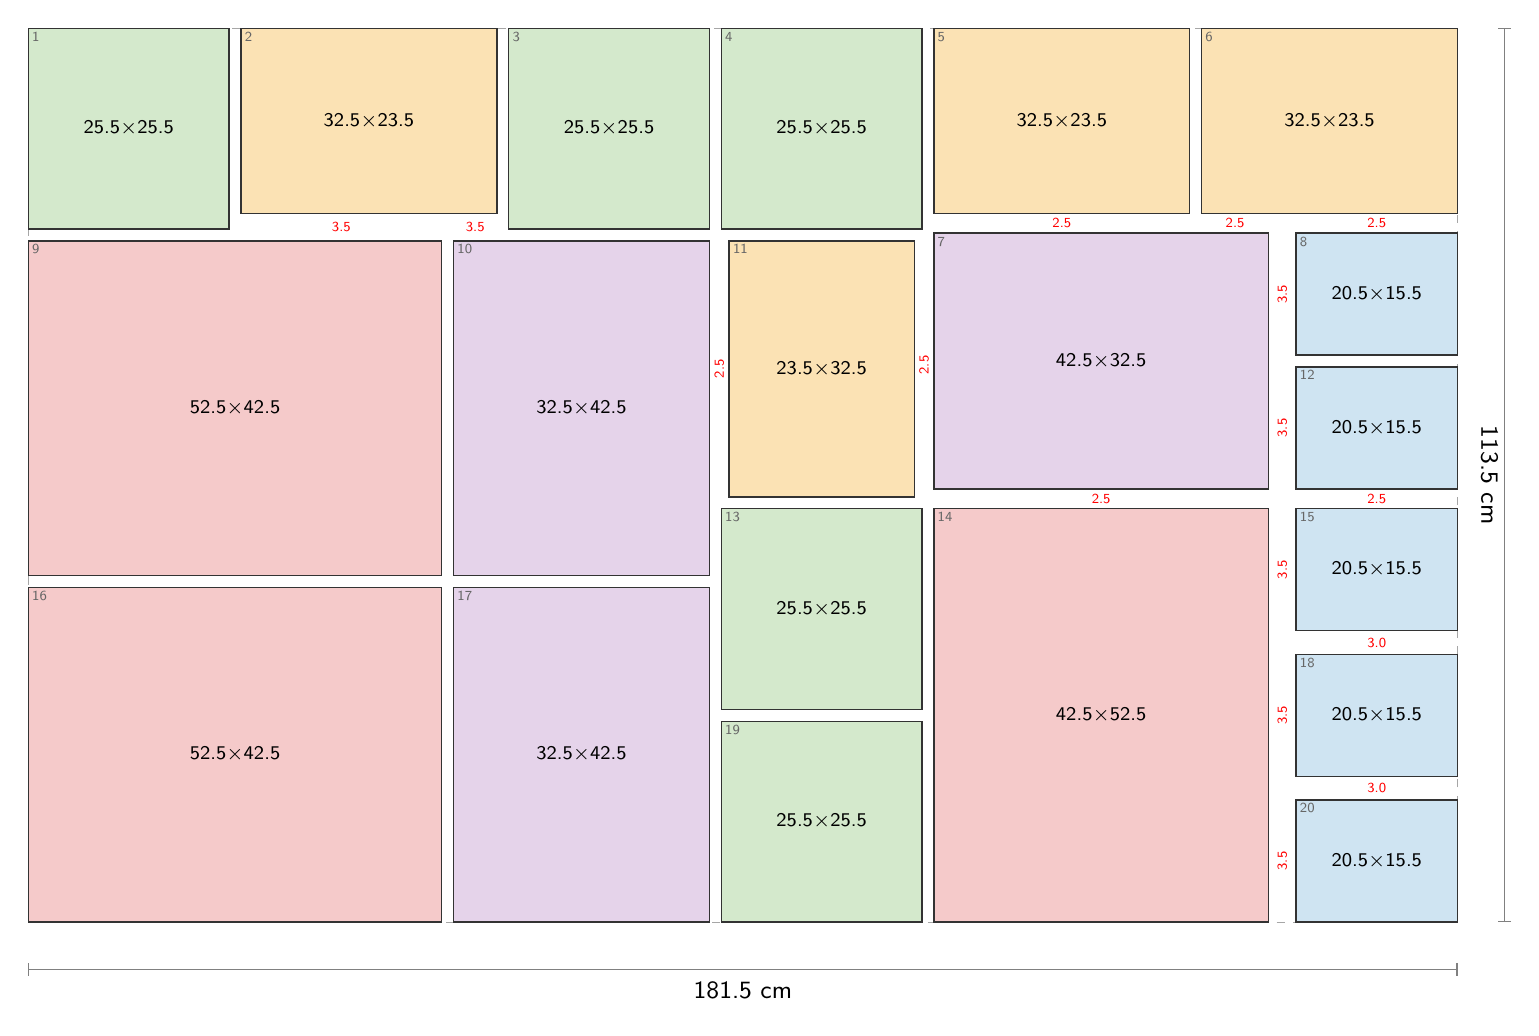
\begin{tikzpicture}[x=1mm, y=-1mm]
\draw[gray!70, dashed, line width=0.4pt] (0,0) rectangle (181.50,113.50);
\filldraw[fill=ft2, draw=black!80, line width=0.5pt] (0.00,0.00) rectangle (25.50,25.50);
\node[align=center, inner sep=0pt] at (12.75,12.75) {\scriptsize 25.5$\times$25.5};
\node[anchor=north west, inner sep=1.2pt, font=\tiny, text=black!60] at (0.00,0.00) {1};
\filldraw[fill=ft1, draw=black!80, line width=0.5pt] (27.00,0.00) rectangle (59.50,23.50);
\node[align=center, inner sep=0pt] at (43.25,11.75) {\scriptsize 32.5$\times$23.5};
\node[anchor=north west, inner sep=1.2pt, font=\tiny, text=black!60] at (27.00,0.00) {2};
\filldraw[fill=ft2, draw=black!80, line width=0.5pt] (61.00,0.00) rectangle (86.50,25.50);
\node[align=center, inner sep=0pt] at (73.75,12.75) {\scriptsize 25.5$\times$25.5};
\node[anchor=north west, inner sep=1.2pt, font=\tiny, text=black!60] at (61.00,0.00) {3};
\filldraw[fill=ft2, draw=black!80, line width=0.5pt] (88.00,0.00) rectangle (113.50,25.50);
\node[align=center, inner sep=0pt] at (100.75,12.75) {\scriptsize 25.5$\times$25.5};
\node[anchor=north west, inner sep=1.2pt, font=\tiny, text=black!60] at (88.00,0.00) {4};
\filldraw[fill=ft1, draw=black!80, line width=0.5pt] (115.00,0.00) rectangle (147.50,23.50);
\node[align=center, inner sep=0pt] at (131.25,11.75) {\scriptsize 32.5$\times$23.5};
\node[anchor=north west, inner sep=1.2pt, font=\tiny, text=black!60] at (115.00,0.00) {5};
\filldraw[fill=ft1, draw=black!80, line width=0.5pt] (149.00,0.00) rectangle (181.50,23.50);
\node[align=center, inner sep=0pt] at (165.25,11.75) {\scriptsize 32.5$\times$23.5};
\node[anchor=north west, inner sep=1.2pt, font=\tiny, text=black!60] at (149.00,0.00) {6};
\filldraw[fill=ft3, draw=black!80, line width=0.5pt] (115.00,26.00) rectangle (157.50,58.50);
\node[align=center, inner sep=0pt] at (136.25,42.25) {\scriptsize 42.5$\times$32.5};
\node[anchor=north west, inner sep=1.2pt, font=\tiny, text=black!60] at (115.00,26.00) {7};
\filldraw[fill=ft0, draw=black!80, line width=0.5pt] (161.00,26.00) rectangle (181.50,41.50);
\node[align=center, inner sep=0pt] at (171.25,33.75) {\scriptsize 20.5$\times$15.5};
\node[anchor=north west, inner sep=1.2pt, font=\tiny, text=black!60] at (161.00,26.00) {8};
\filldraw[fill=ft4, draw=black!80, line width=0.5pt] (0.00,27.00) rectangle (52.50,69.50);
\node[align=center, inner sep=0pt] at (26.25,48.25) {\scriptsize 52.5$\times$42.5};
\node[anchor=north west, inner sep=1.2pt, font=\tiny, text=black!60] at (0.00,27.00) {9};
\filldraw[fill=ft3, draw=black!80, line width=0.5pt] (54.00,27.00) rectangle (86.50,69.50);
\node[align=center, inner sep=0pt] at (70.25,48.25) {\scriptsize 32.5$\times$42.5};
\node[anchor=north west, inner sep=1.2pt, font=\tiny, text=black!60] at (54.00,27.00) {10};
\filldraw[fill=ft1, draw=black!80, line width=0.5pt] (89.00,27.00) rectangle (112.50,59.50);
\node[align=center, inner sep=0pt] at (100.75,43.25) {\scriptsize 23.5$\times$32.5};
\node[anchor=north west, inner sep=1.2pt, font=\tiny, text=black!60] at (89.00,27.00) {11};
\filldraw[fill=ft0, draw=black!80, line width=0.5pt] (161.00,43.00) rectangle (181.50,58.50);
\node[align=center, inner sep=0pt] at (171.25,50.75) {\scriptsize 20.5$\times$15.5};
\node[anchor=north west, inner sep=1.2pt, font=\tiny, text=black!60] at (161.00,43.00) {12};
\filldraw[fill=ft2, draw=black!80, line width=0.5pt] (88.00,61.00) rectangle (113.50,86.50);
\node[align=center, inner sep=0pt] at (100.75,73.75) {\scriptsize 25.5$\times$25.5};
\node[anchor=north west, inner sep=1.2pt, font=\tiny, text=black!60] at (88.00,61.00) {13};
\filldraw[fill=ft4, draw=black!80, line width=0.5pt] (115.00,61.00) rectangle (157.50,113.50);
\node[align=center, inner sep=0pt] at (136.25,87.25) {\scriptsize 42.5$\times$52.5};
\node[anchor=north west, inner sep=1.2pt, font=\tiny, text=black!60] at (115.00,61.00) {14};
\filldraw[fill=ft0, draw=black!80, line width=0.5pt] (161.00,61.00) rectangle (181.50,76.50);
\node[align=center, inner sep=0pt] at (171.25,68.75) {\scriptsize 20.5$\times$15.5};
\node[anchor=north west, inner sep=1.2pt, font=\tiny, text=black!60] at (161.00,61.00) {15};
\filldraw[fill=ft4, draw=black!80, line width=0.5pt] (0.00,71.00) rectangle (52.50,113.50);
\node[align=center, inner sep=0pt] at (26.25,92.25) {\scriptsize 52.5$\times$42.5};
\node[anchor=north west, inner sep=1.2pt, font=\tiny, text=black!60] at (0.00,71.00) {16};
\filldraw[fill=ft3, draw=black!80, line width=0.5pt] (54.00,71.00) rectangle (86.50,113.50);
\node[align=center, inner sep=0pt] at (70.25,92.25) {\scriptsize 32.5$\times$42.5};
\node[anchor=north west, inner sep=1.2pt, font=\tiny, text=black!60] at (54.00,71.00) {17};
\filldraw[fill=ft0, draw=black!80, line width=0.5pt] (161.00,79.50) rectangle (181.50,95.00);
\node[align=center, inner sep=0pt] at (171.25,87.25) {\scriptsize 20.5$\times$15.5};
\node[anchor=north west, inner sep=1.2pt, font=\tiny, text=black!60] at (161.00,79.50) {18};
\filldraw[fill=ft2, draw=black!80, line width=0.5pt] (88.00,88.00) rectangle (113.50,113.50);
\node[align=center, inner sep=0pt] at (100.75,100.75) {\scriptsize 25.5$\times$25.5};
\node[anchor=north west, inner sep=1.2pt, font=\tiny, text=black!60] at (88.00,88.00) {19};
\filldraw[fill=ft0, draw=black!80, line width=0.5pt] (161.00,98.00) rectangle (181.50,113.50);
\node[align=center, inner sep=0pt] at (171.25,105.75) {\scriptsize 20.5$\times$15.5};
\node[anchor=north west, inner sep=1.2pt, font=\tiny, text=black!60] at (161.00,98.00) {20};
\node[font=\tiny, text=red, fill=white, inner sep=0.3pt] at (39.75,25.25) {3.5};
\node[font=\tiny, text=red, fill=white, inner sep=0.3pt] at (56.75,25.25) {3.5};
\node[font=\tiny, text=red, fill=white, inner sep=0.3pt] at (131.25,24.75) {2.5};
\node[font=\tiny, text=red, fill=white, inner sep=0.3pt] at (153.25,24.75) {2.5};
\node[font=\tiny, text=red, fill=white, inner sep=0.3pt] at (171.25,24.75) {2.5};
\node[font=\tiny, text=red, fill=white, inner sep=0.3pt, rotate=90] at (159.25,33.75) {3.5};
\node[font=\tiny, text=red, fill=white, inner sep=0.3pt, rotate=90] at (159.25,50.75) {3.5};
\node[font=\tiny, text=red, fill=white, inner sep=0.3pt] at (136.25,59.75) {2.5};
\node[font=\tiny, text=red, fill=white, inner sep=0.3pt, rotate=90] at (87.75,43.25) {2.5};
\node[font=\tiny, text=red, fill=white, inner sep=0.3pt, rotate=90] at (113.75,42.75) {2.5};
\node[font=\tiny, text=red, fill=white, inner sep=0.3pt] at (171.25,59.75) {2.5};
\node[font=\tiny, text=red, fill=white, inner sep=0.3pt, rotate=90] at (159.25,68.75) {3.5};
\node[font=\tiny, text=red, fill=white, inner sep=0.3pt, rotate=90] at (159.25,87.25) {3.5};
\node[font=\tiny, text=red, fill=white, inner sep=0.3pt, rotate=90] at (159.25,105.75) {3.5};
\node[font=\tiny, text=red, fill=white, inner sep=0.3pt] at (171.25,78.00) {3.0};
\node[font=\tiny, text=red, fill=white, inner sep=0.3pt] at (171.25,96.50) {3.0};
\draw[Bar-Bar, gray] (0,119.50) -- (181.50,119.50) node[midway, below=1pt, font=\small, text=black] {181.5 cm};
\draw[Bar-Bar, gray] (187.50,0) -- (187.50,113.50) node[midway, right=1pt, font=\small, text=black, rotate=-90, anchor=north] {113.5 cm};
\end{tikzpicture}\\[4pt]
{\scriptsize Scale 1:10 (1 mm = 1 cm). Red numbers mark gaps that deviate from the nominal gap by more than 0.25 cm. Small grey numbers index the coordinate table.}
\end{minipage}\hfill
\begin{minipage}[t]{0.25\textwidth}\vspace{0pt}
\small
\begin{tabular}{@{}l l@{}}
\toprule
Outer size & 181.5 $\times$ 113.5 cm \\
Nominal gap & 1.5 cm \\
Actual gaps & 1.5 -- 3.5 cm \\
Max.\ deviation & 2.0 cm \\
Mean deviation & 0.67 cm \\
Border notches & bottom 4 cm, right 6 cm \\
Corners filled & 4 / 4 \\
Frames used & 20 of 28 \\
Large frames & {\scriptsize 3, touching 1$\times$ (52 cm), min.\ dist.\ 44 cm} \\
Entropy & 0.64 \\
\quad {\scriptsize mix / variety} & {\scriptsize 0.86 / 0.74} \\
\quad {\scriptsize stagger / lines} & {\scriptsize 0.46 / 0.50 (3 through)} \\
\bottomrule
\end{tabular}

\vspace{8pt}
\scriptsize
\begin{tabular}{@{}c l l r r@{}}
\toprule
 & outer w $\times$ h (cm) &  & used & have \\
\midrule
\tikz[baseline=-0.6ex]\fill[ft0,draw=black!60] (0,0) rectangle (1.2ex,1.2ex); & 20.5$\times$15.5 & L & 5 & 9 \\
\tikz[baseline=-0.6ex]\fill[ft0,draw=black!60] (0,0) rectangle (1.2ex,1.2ex); & 15.5$\times$20.5 & P & 0 & 2 \\
\tikz[baseline=-0.6ex]\fill[ft3,draw=black!60] (0,0) rectangle (1.2ex,1.2ex); & 32.5$\times$42.5 & P & 2 & 2 \\
\tikz[baseline=-0.6ex]\fill[ft3,draw=black!60] (0,0) rectangle (1.2ex,1.2ex); & 42.5$\times$32.5 & L & 1 & 1 \\
\tikz[baseline=-0.6ex]\fill[ft1,draw=black!60] (0,0) rectangle (1.2ex,1.2ex); & 32.5$\times$23.5 & L & 3 & 5 \\
\tikz[baseline=-0.6ex]\fill[ft1,draw=black!60] (0,0) rectangle (1.2ex,1.2ex); & 23.5$\times$32.5 & P & 1 & 1 \\
\tikz[baseline=-0.6ex]\fill[ft2,draw=black!60] (0,0) rectangle (1.2ex,1.2ex); & 25.5$\times$25.5 &  & 5 & 5 \\
\tikz[baseline=-0.6ex]\fill[ft4,draw=black!60] (0,0) rectangle (1.2ex,1.2ex); & 42.5$\times$52.5 & P & 1 & 1 \\
\tikz[baseline=-0.6ex]\fill[ft4,draw=black!60] (0,0) rectangle (1.2ex,1.2ex); & 52.5$\times$42.5 & L & 2 & 2 \\
\bottomrule
\end{tabular}

\vspace{8pt}
{\bfseries Positions} (top-left corner, cm)\\[2pt]
\tiny
\begin{tabular}{@{}r l r r@{}}
\toprule
\# & frame w $\times$ h & x & y \\
\midrule
1 & 25.5 $\times$ 25.5 & 0.0 & 0.0 \\
2 & 32.5 $\times$ 23.5 & 27.0 & 0.0 \\
3 & 25.5 $\times$ 25.5 & 61.0 & 0.0 \\
4 & 25.5 $\times$ 25.5 & 88.0 & 0.0 \\
5 & 32.5 $\times$ 23.5 & 115.0 & 0.0 \\
6 & 32.5 $\times$ 23.5 & 149.0 & 0.0 \\
7 & 42.5 $\times$ 32.5 & 115.0 & 26.0 \\
8 & 20.5 $\times$ 15.5 & 161.0 & 26.0 \\
9 & 52.5 $\times$ 42.5 & 0.0 & 27.0 \\
10 & 32.5 $\times$ 42.5 & 54.0 & 27.0 \\
11 & 23.5 $\times$ 32.5 & 89.0 & 27.0 \\
12 & 20.5 $\times$ 15.5 & 161.0 & 43.0 \\
13 & 25.5 $\times$ 25.5 & 88.0 & 61.0 \\
14 & 42.5 $\times$ 52.5 & 115.0 & 61.0 \\
15 & 20.5 $\times$ 15.5 & 161.0 & 61.0 \\
16 & 52.5 $\times$ 42.5 & 0.0 & 71.0 \\
17 & 32.5 $\times$ 42.5 & 54.0 & 71.0 \\
18 & 20.5 $\times$ 15.5 & 161.0 & 79.5 \\
19 & 25.5 $\times$ 25.5 & 88.0 & 88.0 \\
20 & 20.5 $\times$ 15.5 & 161.0 & 98.0 \\
\bottomrule
\end{tabular}
\end{minipage}
\clearpage

\phantomsection\addcontentsline{toc}{subsection}{Layout 15: 191.0 \texorpdfstring{$\times$}{x} 103.5 cm, 16 frames, gap 6 cm, max.\ deviation 3.5 cm}
\label{lay:per-run-gap:15}
\begin{minipage}[t]{0.74\textwidth}\vspace{0pt}
{\LARGE\bfseries Layout 15}\hspace{1.5em}{\large 191.0 $\times$ 103.5 cm \quad gap 6 cm \quad 16 frames}\\[8pt]
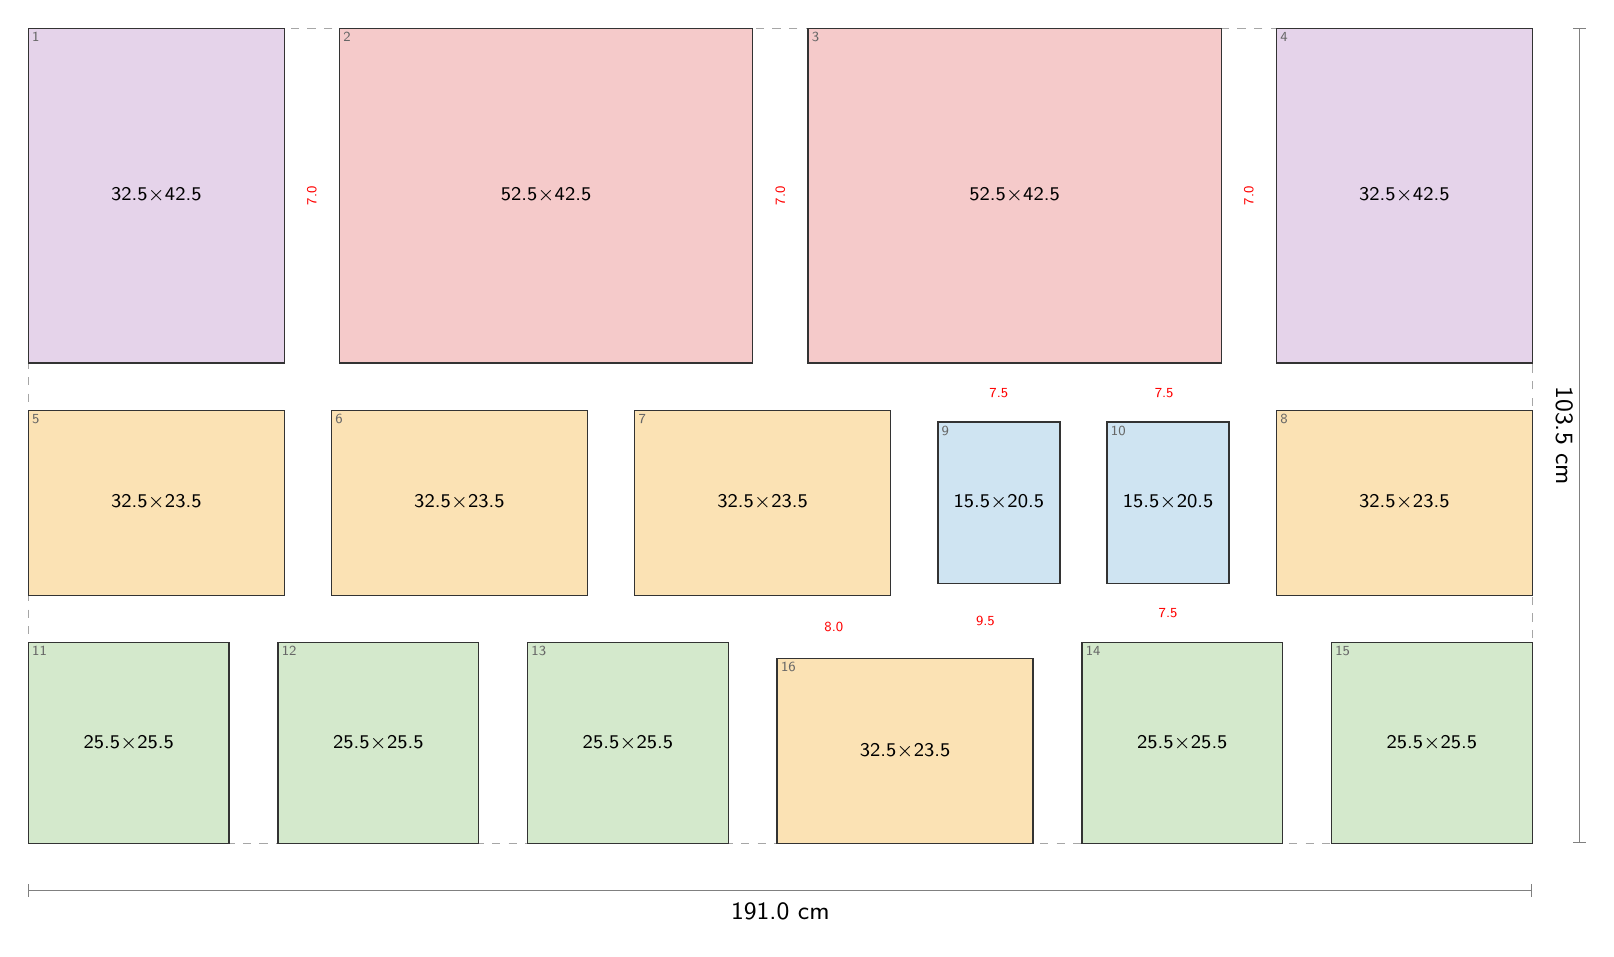
\begin{tikzpicture}[x=1mm, y=-1mm]
\draw[gray!70, dashed, line width=0.4pt] (0,0) rectangle (191.00,103.50);
\filldraw[fill=ft3, draw=black!80, line width=0.5pt] (0.00,0.00) rectangle (32.50,42.50);
\node[align=center, inner sep=0pt] at (16.25,21.25) {\scriptsize 32.5$\times$42.5};
\node[anchor=north west, inner sep=1.2pt, font=\tiny, text=black!60] at (0.00,0.00) {1};
\filldraw[fill=ft4, draw=black!80, line width=0.5pt] (39.50,0.00) rectangle (92.00,42.50);
\node[align=center, inner sep=0pt] at (65.75,21.25) {\scriptsize 52.5$\times$42.5};
\node[anchor=north west, inner sep=1.2pt, font=\tiny, text=black!60] at (39.50,0.00) {2};
\filldraw[fill=ft4, draw=black!80, line width=0.5pt] (99.00,0.00) rectangle (151.50,42.50);
\node[align=center, inner sep=0pt] at (125.25,21.25) {\scriptsize 52.5$\times$42.5};
\node[anchor=north west, inner sep=1.2pt, font=\tiny, text=black!60] at (99.00,0.00) {3};
\filldraw[fill=ft3, draw=black!80, line width=0.5pt] (158.50,0.00) rectangle (191.00,42.50);
\node[align=center, inner sep=0pt] at (174.75,21.25) {\scriptsize 32.5$\times$42.5};
\node[anchor=north west, inner sep=1.2pt, font=\tiny, text=black!60] at (158.50,0.00) {4};
\filldraw[fill=ft1, draw=black!80, line width=0.5pt] (0.00,48.50) rectangle (32.50,72.00);
\node[align=center, inner sep=0pt] at (16.25,60.25) {\scriptsize 32.5$\times$23.5};
\node[anchor=north west, inner sep=1.2pt, font=\tiny, text=black!60] at (0.00,48.50) {5};
\filldraw[fill=ft1, draw=black!80, line width=0.5pt] (38.50,48.50) rectangle (71.00,72.00);
\node[align=center, inner sep=0pt] at (54.75,60.25) {\scriptsize 32.5$\times$23.5};
\node[anchor=north west, inner sep=1.2pt, font=\tiny, text=black!60] at (38.50,48.50) {6};
\filldraw[fill=ft1, draw=black!80, line width=0.5pt] (77.00,48.50) rectangle (109.50,72.00);
\node[align=center, inner sep=0pt] at (93.25,60.25) {\scriptsize 32.5$\times$23.5};
\node[anchor=north west, inner sep=1.2pt, font=\tiny, text=black!60] at (77.00,48.50) {7};
\filldraw[fill=ft1, draw=black!80, line width=0.5pt] (158.50,48.50) rectangle (191.00,72.00);
\node[align=center, inner sep=0pt] at (174.75,60.25) {\scriptsize 32.5$\times$23.5};
\node[anchor=north west, inner sep=1.2pt, font=\tiny, text=black!60] at (158.50,48.50) {8};
\filldraw[fill=ft0, draw=black!80, line width=0.5pt] (115.50,50.00) rectangle (131.00,70.50);
\node[align=center, inner sep=0pt] at (123.25,60.25) {\scriptsize 15.5$\times$20.5};
\node[anchor=north west, inner sep=1.2pt, font=\tiny, text=black!60] at (115.50,50.00) {9};
\filldraw[fill=ft0, draw=black!80, line width=0.5pt] (137.00,50.00) rectangle (152.50,70.50);
\node[align=center, inner sep=0pt] at (144.75,60.25) {\scriptsize 15.5$\times$20.5};
\node[anchor=north west, inner sep=1.2pt, font=\tiny, text=black!60] at (137.00,50.00) {10};
\filldraw[fill=ft2, draw=black!80, line width=0.5pt] (0.00,78.00) rectangle (25.50,103.50);
\node[align=center, inner sep=0pt] at (12.75,90.75) {\scriptsize 25.5$\times$25.5};
\node[anchor=north west, inner sep=1.2pt, font=\tiny, text=black!60] at (0.00,78.00) {11};
\filldraw[fill=ft2, draw=black!80, line width=0.5pt] (31.70,78.00) rectangle (57.20,103.50);
\node[align=center, inner sep=0pt] at (44.45,90.75) {\scriptsize 25.5$\times$25.5};
\node[anchor=north west, inner sep=1.2pt, font=\tiny, text=black!60] at (31.70,78.00) {12};
\filldraw[fill=ft2, draw=black!80, line width=0.5pt] (63.40,78.00) rectangle (88.90,103.50);
\node[align=center, inner sep=0pt] at (76.15,90.75) {\scriptsize 25.5$\times$25.5};
\node[anchor=north west, inner sep=1.2pt, font=\tiny, text=black!60] at (63.40,78.00) {13};
\filldraw[fill=ft2, draw=black!80, line width=0.5pt] (133.80,78.00) rectangle (159.30,103.50);
\node[align=center, inner sep=0pt] at (146.55,90.75) {\scriptsize 25.5$\times$25.5};
\node[anchor=north west, inner sep=1.2pt, font=\tiny, text=black!60] at (133.80,78.00) {14};
\filldraw[fill=ft2, draw=black!80, line width=0.5pt] (165.50,78.00) rectangle (191.00,103.50);
\node[align=center, inner sep=0pt] at (178.25,90.75) {\scriptsize 25.5$\times$25.5};
\node[anchor=north west, inner sep=1.2pt, font=\tiny, text=black!60] at (165.50,78.00) {15};
\filldraw[fill=ft1, draw=black!80, line width=0.5pt] (95.10,80.00) rectangle (127.60,103.50);
\node[align=center, inner sep=0pt] at (111.35,91.75) {\scriptsize 32.5$\times$23.5};
\node[anchor=north west, inner sep=1.2pt, font=\tiny, text=black!60] at (95.10,80.00) {16};
\node[font=\tiny, text=red, fill=white, inner sep=0.3pt, rotate=90] at (36.00,21.25) {7.0};
\node[font=\tiny, text=red, fill=white, inner sep=0.3pt, rotate=90] at (95.50,21.25) {7.0};
\node[font=\tiny, text=red, fill=white, inner sep=0.3pt, rotate=90] at (155.00,21.25) {7.0};
\node[font=\tiny, text=red, fill=white, inner sep=0.3pt] at (123.25,46.25) {7.5};
\node[font=\tiny, text=red, fill=white, inner sep=0.3pt] at (144.25,46.25) {7.5};
\node[font=\tiny, text=red, fill=white, inner sep=0.3pt] at (102.30,76.00) {8.0};
\node[font=\tiny, text=red, fill=white, inner sep=0.3pt] at (121.55,75.25) {9.5};
\node[font=\tiny, text=red, fill=white, inner sep=0.3pt] at (144.75,74.25) {7.5};
\draw[Bar-Bar, gray] (0,109.50) -- (191.00,109.50) node[midway, below=1pt, font=\small, text=black] {191.0 cm};
\draw[Bar-Bar, gray] (197.00,0) -- (197.00,103.50) node[midway, right=1pt, font=\small, text=black, rotate=-90, anchor=north] {103.5 cm};
\end{tikzpicture}\\[4pt]
{\scriptsize Scale 1:10 (1 mm = 1 cm). Red numbers mark gaps that deviate from the nominal gap by more than 0.25 cm. Small grey numbers index the coordinate table.}
\end{minipage}\hfill
\begin{minipage}[t]{0.25\textwidth}\vspace{0pt}
\small
\begin{tabular}{@{}l l@{}}
\toprule
Outer size & 191.0 $\times$ 103.5 cm \\
Nominal gap & 6 cm \\
Actual gaps & 6.0 -- 9.5 cm \\
Max.\ deviation & 3.5 cm \\
Mean deviation & 0.50 cm \\
Border notches & none \\
Corners filled & 4 / 4 \\
Frames used & 16 of 28 \\
Large frames & {\scriptsize 2, touching 1$\times$ (42 cm), min.\ dist.\ 60 cm} \\
Entropy & 0.67 \\
\quad {\scriptsize mix / variety} & {\scriptsize 0.69 / 0.70} \\
\quad {\scriptsize stagger / lines} & {\scriptsize 0.55 / 0.75 (2 through)} \\
\bottomrule
\end{tabular}

\vspace{8pt}
\scriptsize
\begin{tabular}{@{}c l l r r@{}}
\toprule
 & outer w $\times$ h (cm) &  & used & have \\
\midrule
\tikz[baseline=-0.6ex]\fill[ft0,draw=black!60] (0,0) rectangle (1.2ex,1.2ex); & 20.5$\times$15.5 & L & 0 & 9 \\
\tikz[baseline=-0.6ex]\fill[ft0,draw=black!60] (0,0) rectangle (1.2ex,1.2ex); & 15.5$\times$20.5 & P & 2 & 2 \\
\tikz[baseline=-0.6ex]\fill[ft3,draw=black!60] (0,0) rectangle (1.2ex,1.2ex); & 32.5$\times$42.5 & P & 2 & 2 \\
\tikz[baseline=-0.6ex]\fill[ft3,draw=black!60] (0,0) rectangle (1.2ex,1.2ex); & 42.5$\times$32.5 & L & 0 & 1 \\
\tikz[baseline=-0.6ex]\fill[ft1,draw=black!60] (0,0) rectangle (1.2ex,1.2ex); & 32.5$\times$23.5 & L & 5 & 5 \\
\tikz[baseline=-0.6ex]\fill[ft1,draw=black!60] (0,0) rectangle (1.2ex,1.2ex); & 23.5$\times$32.5 & P & 0 & 1 \\
\tikz[baseline=-0.6ex]\fill[ft2,draw=black!60] (0,0) rectangle (1.2ex,1.2ex); & 25.5$\times$25.5 &  & 5 & 5 \\
\tikz[baseline=-0.6ex]\fill[ft4,draw=black!60] (0,0) rectangle (1.2ex,1.2ex); & 42.5$\times$52.5 & P & 0 & 1 \\
\tikz[baseline=-0.6ex]\fill[ft4,draw=black!60] (0,0) rectangle (1.2ex,1.2ex); & 52.5$\times$42.5 & L & 2 & 2 \\
\bottomrule
\end{tabular}

\vspace{8pt}
{\bfseries Positions} (top-left corner, cm)\\[2pt]
\tiny
\begin{tabular}{@{}r l r r@{}}
\toprule
\# & frame w $\times$ h & x & y \\
\midrule
1 & 32.5 $\times$ 42.5 & 0.0 & 0.0 \\
2 & 52.5 $\times$ 42.5 & 39.5 & 0.0 \\
3 & 52.5 $\times$ 42.5 & 99.0 & 0.0 \\
4 & 32.5 $\times$ 42.5 & 158.5 & 0.0 \\
5 & 32.5 $\times$ 23.5 & 0.0 & 48.5 \\
6 & 32.5 $\times$ 23.5 & 38.5 & 48.5 \\
7 & 32.5 $\times$ 23.5 & 77.0 & 48.5 \\
8 & 32.5 $\times$ 23.5 & 158.5 & 48.5 \\
9 & 15.5 $\times$ 20.5 & 115.5 & 50.0 \\
10 & 15.5 $\times$ 20.5 & 137.0 & 50.0 \\
11 & 25.5 $\times$ 25.5 & 0.0 & 78.0 \\
12 & 25.5 $\times$ 25.5 & 31.7 & 78.0 \\
13 & 25.5 $\times$ 25.5 & 63.4 & 78.0 \\
14 & 25.5 $\times$ 25.5 & 133.8 & 78.0 \\
15 & 25.5 $\times$ 25.5 & 165.5 & 78.0 \\
16 & 32.5 $\times$ 23.5 & 95.1 & 80.0 \\
\bottomrule
\end{tabular}
\end{minipage}
\clearpage

\phantomsection\addcontentsline{toc}{subsection}{Layout 16: 182.5 \texorpdfstring{$\times$}{x} 123.5 cm, 26 frames, gap 1.5 cm, max.\ deviation 5.0 cm}
\label{lay:per-run-gap:16}
\begin{minipage}[t]{0.74\textwidth}\vspace{0pt}
{\LARGE\bfseries Layout 16}\hspace{1.5em}{\large 182.5 $\times$ 123.5 cm \quad gap 1.5 cm \quad 26 frames}\\[8pt]
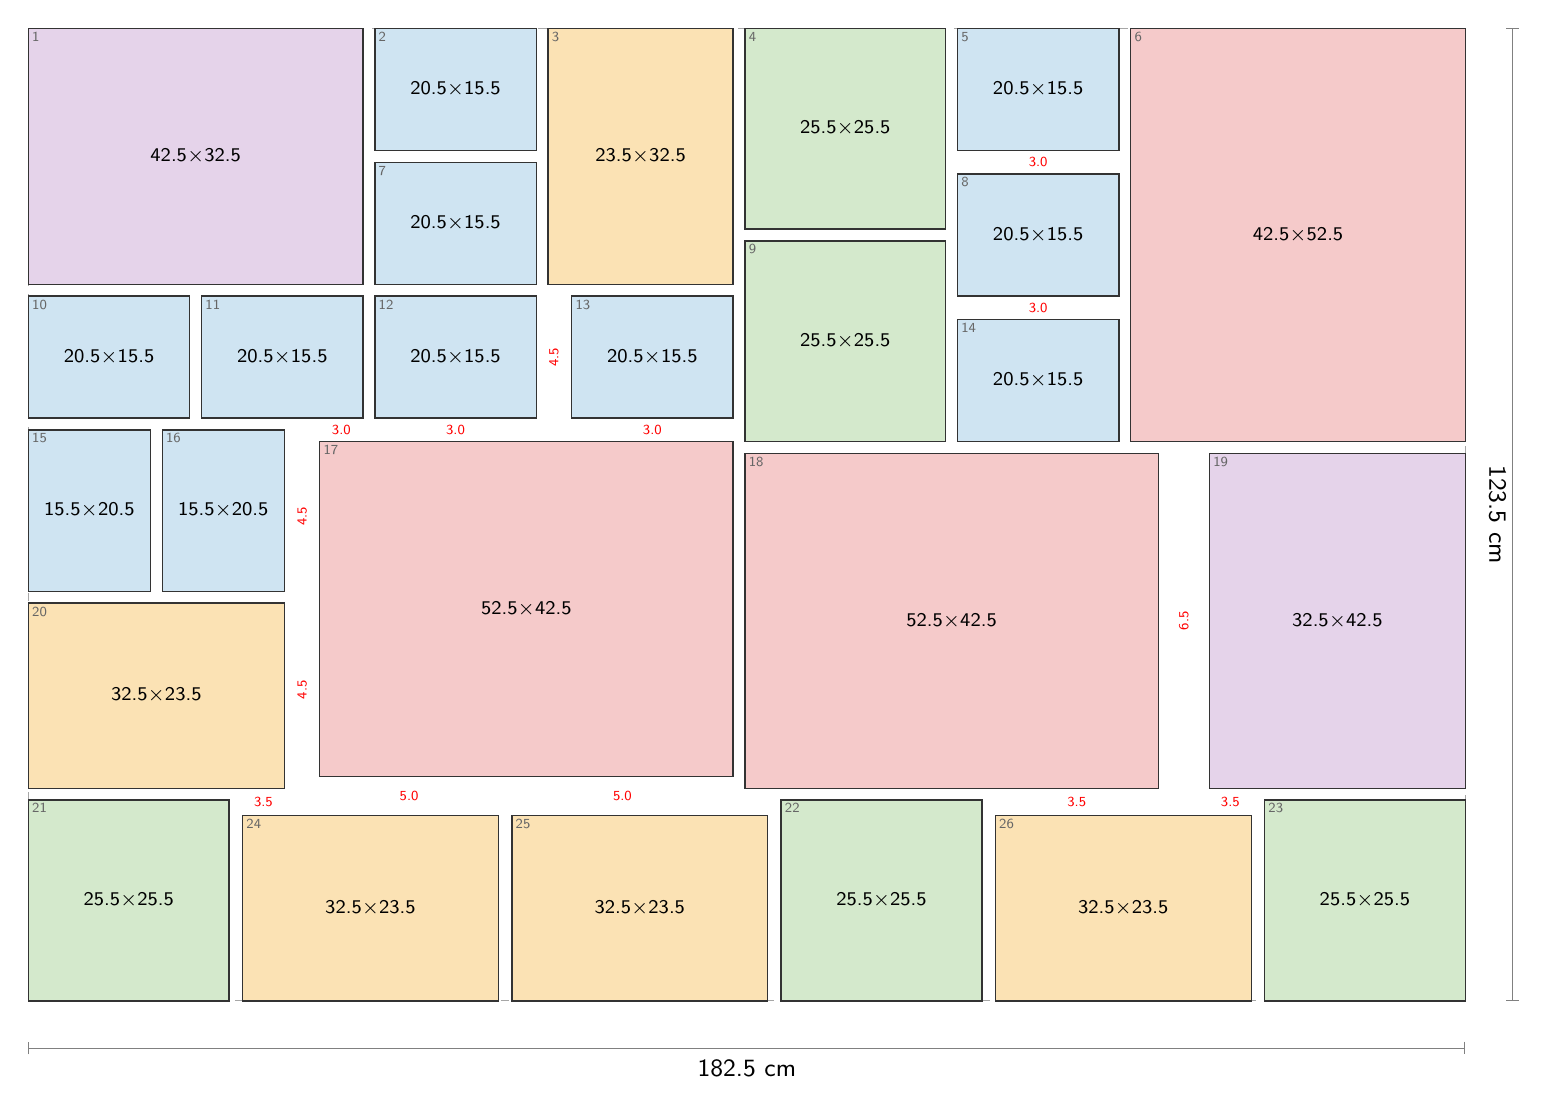
\begin{tikzpicture}[x=1mm, y=-1mm]
\draw[gray!70, dashed, line width=0.4pt] (0,0) rectangle (182.50,123.50);
\filldraw[fill=ft3, draw=black!80, line width=0.5pt] (0.00,0.00) rectangle (42.50,32.50);
\node[align=center, inner sep=0pt] at (21.25,16.25) {\scriptsize 42.5$\times$32.5};
\node[anchor=north west, inner sep=1.2pt, font=\tiny, text=black!60] at (0.00,0.00) {1};
\filldraw[fill=ft0, draw=black!80, line width=0.5pt] (44.00,0.00) rectangle (64.50,15.50);
\node[align=center, inner sep=0pt] at (54.25,7.75) {\scriptsize 20.5$\times$15.5};
\node[anchor=north west, inner sep=1.2pt, font=\tiny, text=black!60] at (44.00,0.00) {2};
\filldraw[fill=ft1, draw=black!80, line width=0.5pt] (66.00,0.00) rectangle (89.50,32.50);
\node[align=center, inner sep=0pt] at (77.75,16.25) {\scriptsize 23.5$\times$32.5};
\node[anchor=north west, inner sep=1.2pt, font=\tiny, text=black!60] at (66.00,0.00) {3};
\filldraw[fill=ft2, draw=black!80, line width=0.5pt] (91.00,0.00) rectangle (116.50,25.50);
\node[align=center, inner sep=0pt] at (103.75,12.75) {\scriptsize 25.5$\times$25.5};
\node[anchor=north west, inner sep=1.2pt, font=\tiny, text=black!60] at (91.00,0.00) {4};
\filldraw[fill=ft0, draw=black!80, line width=0.5pt] (118.00,0.00) rectangle (138.50,15.50);
\node[align=center, inner sep=0pt] at (128.25,7.75) {\scriptsize 20.5$\times$15.5};
\node[anchor=north west, inner sep=1.2pt, font=\tiny, text=black!60] at (118.00,0.00) {5};
\filldraw[fill=ft4, draw=black!80, line width=0.5pt] (140.00,0.00) rectangle (182.50,52.50);
\node[align=center, inner sep=0pt] at (161.25,26.25) {\scriptsize 42.5$\times$52.5};
\node[anchor=north west, inner sep=1.2pt, font=\tiny, text=black!60] at (140.00,0.00) {6};
\filldraw[fill=ft0, draw=black!80, line width=0.5pt] (44.00,17.00) rectangle (64.50,32.50);
\node[align=center, inner sep=0pt] at (54.25,24.75) {\scriptsize 20.5$\times$15.5};
\node[anchor=north west, inner sep=1.2pt, font=\tiny, text=black!60] at (44.00,17.00) {7};
\filldraw[fill=ft0, draw=black!80, line width=0.5pt] (118.00,18.50) rectangle (138.50,34.00);
\node[align=center, inner sep=0pt] at (128.25,26.25) {\scriptsize 20.5$\times$15.5};
\node[anchor=north west, inner sep=1.2pt, font=\tiny, text=black!60] at (118.00,18.50) {8};
\filldraw[fill=ft2, draw=black!80, line width=0.5pt] (91.00,27.00) rectangle (116.50,52.50);
\node[align=center, inner sep=0pt] at (103.75,39.75) {\scriptsize 25.5$\times$25.5};
\node[anchor=north west, inner sep=1.2pt, font=\tiny, text=black!60] at (91.00,27.00) {9};
\filldraw[fill=ft0, draw=black!80, line width=0.5pt] (0.00,34.00) rectangle (20.50,49.50);
\node[align=center, inner sep=0pt] at (10.25,41.75) {\scriptsize 20.5$\times$15.5};
\node[anchor=north west, inner sep=1.2pt, font=\tiny, text=black!60] at (0.00,34.00) {10};
\filldraw[fill=ft0, draw=black!80, line width=0.5pt] (22.00,34.00) rectangle (42.50,49.50);
\node[align=center, inner sep=0pt] at (32.25,41.75) {\scriptsize 20.5$\times$15.5};
\node[anchor=north west, inner sep=1.2pt, font=\tiny, text=black!60] at (22.00,34.00) {11};
\filldraw[fill=ft0, draw=black!80, line width=0.5pt] (44.00,34.00) rectangle (64.50,49.50);
\node[align=center, inner sep=0pt] at (54.25,41.75) {\scriptsize 20.5$\times$15.5};
\node[anchor=north west, inner sep=1.2pt, font=\tiny, text=black!60] at (44.00,34.00) {12};
\filldraw[fill=ft0, draw=black!80, line width=0.5pt] (69.00,34.00) rectangle (89.50,49.50);
\node[align=center, inner sep=0pt] at (79.25,41.75) {\scriptsize 20.5$\times$15.5};
\node[anchor=north west, inner sep=1.2pt, font=\tiny, text=black!60] at (69.00,34.00) {13};
\filldraw[fill=ft0, draw=black!80, line width=0.5pt] (118.00,37.00) rectangle (138.50,52.50);
\node[align=center, inner sep=0pt] at (128.25,44.75) {\scriptsize 20.5$\times$15.5};
\node[anchor=north west, inner sep=1.2pt, font=\tiny, text=black!60] at (118.00,37.00) {14};
\filldraw[fill=ft0, draw=black!80, line width=0.5pt] (0.00,51.00) rectangle (15.50,71.50);
\node[align=center, inner sep=0pt] at (7.75,61.25) {\scriptsize 15.5$\times$20.5};
\node[anchor=north west, inner sep=1.2pt, font=\tiny, text=black!60] at (0.00,51.00) {15};
\filldraw[fill=ft0, draw=black!80, line width=0.5pt] (17.00,51.00) rectangle (32.50,71.50);
\node[align=center, inner sep=0pt] at (24.75,61.25) {\scriptsize 15.5$\times$20.5};
\node[anchor=north west, inner sep=1.2pt, font=\tiny, text=black!60] at (17.00,51.00) {16};
\filldraw[fill=ft4, draw=black!80, line width=0.5pt] (37.00,52.50) rectangle (89.50,95.00);
\node[align=center, inner sep=0pt] at (63.25,73.75) {\scriptsize 52.5$\times$42.5};
\node[anchor=north west, inner sep=1.2pt, font=\tiny, text=black!60] at (37.00,52.50) {17};
\filldraw[fill=ft4, draw=black!80, line width=0.5pt] (91.00,54.00) rectangle (143.50,96.50);
\node[align=center, inner sep=0pt] at (117.25,75.25) {\scriptsize 52.5$\times$42.5};
\node[anchor=north west, inner sep=1.2pt, font=\tiny, text=black!60] at (91.00,54.00) {18};
\filldraw[fill=ft3, draw=black!80, line width=0.5pt] (150.00,54.00) rectangle (182.50,96.50);
\node[align=center, inner sep=0pt] at (166.25,75.25) {\scriptsize 32.5$\times$42.5};
\node[anchor=north west, inner sep=1.2pt, font=\tiny, text=black!60] at (150.00,54.00) {19};
\filldraw[fill=ft1, draw=black!80, line width=0.5pt] (0.00,73.00) rectangle (32.50,96.50);
\node[align=center, inner sep=0pt] at (16.25,84.75) {\scriptsize 32.5$\times$23.5};
\node[anchor=north west, inner sep=1.2pt, font=\tiny, text=black!60] at (0.00,73.00) {20};
\filldraw[fill=ft2, draw=black!80, line width=0.5pt] (0.00,98.00) rectangle (25.50,123.50);
\node[align=center, inner sep=0pt] at (12.75,110.75) {\scriptsize 25.5$\times$25.5};
\node[anchor=north west, inner sep=1.2pt, font=\tiny, text=black!60] at (0.00,98.00) {21};
\filldraw[fill=ft2, draw=black!80, line width=0.5pt] (95.60,98.00) rectangle (121.10,123.50);
\node[align=center, inner sep=0pt] at (108.35,110.75) {\scriptsize 25.5$\times$25.5};
\node[anchor=north west, inner sep=1.2pt, font=\tiny, text=black!60] at (95.60,98.00) {22};
\filldraw[fill=ft2, draw=black!80, line width=0.5pt] (157.00,98.00) rectangle (182.50,123.50);
\node[align=center, inner sep=0pt] at (169.75,110.75) {\scriptsize 25.5$\times$25.5};
\node[anchor=north west, inner sep=1.2pt, font=\tiny, text=black!60] at (157.00,98.00) {23};
\filldraw[fill=ft1, draw=black!80, line width=0.5pt] (27.20,100.00) rectangle (59.70,123.50);
\node[align=center, inner sep=0pt] at (43.45,111.75) {\scriptsize 32.5$\times$23.5};
\node[anchor=north west, inner sep=1.2pt, font=\tiny, text=black!60] at (27.20,100.00) {24};
\filldraw[fill=ft1, draw=black!80, line width=0.5pt] (61.40,100.00) rectangle (93.90,123.50);
\node[align=center, inner sep=0pt] at (77.65,111.75) {\scriptsize 32.5$\times$23.5};
\node[anchor=north west, inner sep=1.2pt, font=\tiny, text=black!60] at (61.40,100.00) {25};
\filldraw[fill=ft1, draw=black!80, line width=0.5pt] (122.80,100.00) rectangle (155.30,123.50);
\node[align=center, inner sep=0pt] at (139.05,111.75) {\scriptsize 32.5$\times$23.5};
\node[anchor=north west, inner sep=1.2pt, font=\tiny, text=black!60] at (122.80,100.00) {26};
\node[font=\tiny, text=red, fill=white, inner sep=0.3pt] at (128.25,17.00) {3.0};
\node[font=\tiny, text=red, fill=white, inner sep=0.3pt] at (128.25,35.50) {3.0};
\node[font=\tiny, text=red, fill=white, inner sep=0.3pt] at (39.75,51.00) {3.0};
\node[font=\tiny, text=red, fill=white, inner sep=0.3pt, rotate=90] at (66.75,41.75) {4.5};
\node[font=\tiny, text=red, fill=white, inner sep=0.3pt] at (54.25,51.00) {3.0};
\node[font=\tiny, text=red, fill=white, inner sep=0.3pt] at (79.25,51.00) {3.0};
\node[font=\tiny, text=red, fill=white, inner sep=0.3pt, rotate=90] at (34.75,62.00) {4.5};
\node[font=\tiny, text=red, fill=white, inner sep=0.3pt] at (48.35,97.50) {5.0};
\node[font=\tiny, text=red, fill=white, inner sep=0.3pt] at (75.45,97.50) {5.0};
\node[font=\tiny, text=red, fill=white, inner sep=0.3pt, rotate=90] at (146.75,75.25) {6.5};
\node[font=\tiny, text=red, fill=white, inner sep=0.3pt] at (133.15,98.25) {3.5};
\node[font=\tiny, text=red, fill=white, inner sep=0.3pt] at (152.65,98.25) {3.5};
\node[font=\tiny, text=red, fill=white, inner sep=0.3pt, rotate=90] at (34.75,84.00) {4.5};
\node[font=\tiny, text=red, fill=white, inner sep=0.3pt] at (29.85,98.25) {3.5};
\draw[Bar-Bar, gray] (0,129.50) -- (182.50,129.50) node[midway, below=1pt, font=\small, text=black] {182.5 cm};
\draw[Bar-Bar, gray] (188.50,0) -- (188.50,123.50) node[midway, right=1pt, font=\small, text=black, rotate=-90, anchor=north] {123.5 cm};
\end{tikzpicture}\\[4pt]
{\scriptsize Scale 1:10 (1 mm = 1 cm). Red numbers mark gaps that deviate from the nominal gap by more than 0.25 cm. Small grey numbers index the coordinate table.}
\end{minipage}\hfill
\begin{minipage}[t]{0.25\textwidth}\vspace{0pt}
\small
\begin{tabular}{@{}l l@{}}
\toprule
Outer size & 182.5 $\times$ 123.5 cm \\
Nominal gap & 1.5 cm \\
Actual gaps & 1.5 -- 6.5 cm \\
Max.\ deviation & 5.0 cm \\
Mean deviation & 0.67 cm \\
Border notches & none \\
Corners filled & 4 / 4 \\
Frames used & 26 of 28 \\
Large frames & {\scriptsize 3, touching 1$\times$ (41 cm), min.\ dist.\ 54 cm} \\
Entropy & 0.78 \\
\quad {\scriptsize mix / variety} & {\scriptsize 0.85 / 0.79} \\
\quad {\scriptsize stagger / lines} & {\scriptsize 0.49 / 1.00 (1 through)} \\
\bottomrule
\end{tabular}

\vspace{8pt}
\scriptsize
\begin{tabular}{@{}c l l r r@{}}
\toprule
 & outer w $\times$ h (cm) &  & used & have \\
\midrule
\tikz[baseline=-0.6ex]\fill[ft0,draw=black!60] (0,0) rectangle (1.2ex,1.2ex); & 20.5$\times$15.5 & L & 9 & 9 \\
\tikz[baseline=-0.6ex]\fill[ft0,draw=black!60] (0,0) rectangle (1.2ex,1.2ex); & 15.5$\times$20.5 & P & 2 & 2 \\
\tikz[baseline=-0.6ex]\fill[ft3,draw=black!60] (0,0) rectangle (1.2ex,1.2ex); & 32.5$\times$42.5 & P & 1 & 2 \\
\tikz[baseline=-0.6ex]\fill[ft3,draw=black!60] (0,0) rectangle (1.2ex,1.2ex); & 42.5$\times$32.5 & L & 1 & 1 \\
\tikz[baseline=-0.6ex]\fill[ft1,draw=black!60] (0,0) rectangle (1.2ex,1.2ex); & 32.5$\times$23.5 & L & 4 & 5 \\
\tikz[baseline=-0.6ex]\fill[ft1,draw=black!60] (0,0) rectangle (1.2ex,1.2ex); & 23.5$\times$32.5 & P & 1 & 1 \\
\tikz[baseline=-0.6ex]\fill[ft2,draw=black!60] (0,0) rectangle (1.2ex,1.2ex); & 25.5$\times$25.5 &  & 5 & 5 \\
\tikz[baseline=-0.6ex]\fill[ft4,draw=black!60] (0,0) rectangle (1.2ex,1.2ex); & 42.5$\times$52.5 & P & 1 & 1 \\
\tikz[baseline=-0.6ex]\fill[ft4,draw=black!60] (0,0) rectangle (1.2ex,1.2ex); & 52.5$\times$42.5 & L & 2 & 2 \\
\bottomrule
\end{tabular}

\vspace{8pt}
{\bfseries Positions} (top-left corner, cm)\\[2pt]
\tiny
\begin{tabular}{@{}r l r r@{}}
\toprule
\# & frame w $\times$ h & x & y \\
\midrule
1 & 42.5 $\times$ 32.5 & 0.0 & 0.0 \\
2 & 20.5 $\times$ 15.5 & 44.0 & 0.0 \\
3 & 23.5 $\times$ 32.5 & 66.0 & 0.0 \\
4 & 25.5 $\times$ 25.5 & 91.0 & 0.0 \\
5 & 20.5 $\times$ 15.5 & 118.0 & 0.0 \\
6 & 42.5 $\times$ 52.5 & 140.0 & 0.0 \\
7 & 20.5 $\times$ 15.5 & 44.0 & 17.0 \\
8 & 20.5 $\times$ 15.5 & 118.0 & 18.5 \\
9 & 25.5 $\times$ 25.5 & 91.0 & 27.0 \\
10 & 20.5 $\times$ 15.5 & 0.0 & 34.0 \\
11 & 20.5 $\times$ 15.5 & 22.0 & 34.0 \\
12 & 20.5 $\times$ 15.5 & 44.0 & 34.0 \\
13 & 20.5 $\times$ 15.5 & 69.0 & 34.0 \\
14 & 20.5 $\times$ 15.5 & 118.0 & 37.0 \\
15 & 15.5 $\times$ 20.5 & 0.0 & 51.0 \\
16 & 15.5 $\times$ 20.5 & 17.0 & 51.0 \\
17 & 52.5 $\times$ 42.5 & 37.0 & 52.5 \\
18 & 52.5 $\times$ 42.5 & 91.0 & 54.0 \\
19 & 32.5 $\times$ 42.5 & 150.0 & 54.0 \\
20 & 32.5 $\times$ 23.5 & 0.0 & 73.0 \\
21 & 25.5 $\times$ 25.5 & 0.0 & 98.0 \\
22 & 25.5 $\times$ 25.5 & 95.6 & 98.0 \\
23 & 25.5 $\times$ 25.5 & 157.0 & 98.0 \\
24 & 32.5 $\times$ 23.5 & 27.2 & 100.0 \\
25 & 32.5 $\times$ 23.5 & 61.4 & 100.0 \\
26 & 32.5 $\times$ 23.5 & 122.8 & 100.0 \\
\bottomrule
\end{tabular}
\end{minipage}
\clearpage

\section{proportional}\label{sec:proportional}
Unavoidable slack is distributed in proportion to the size of the neighbouring frames: the weight of a gap is the mean extent of the two frames (or groups) it separates, so gaps next to big frames widen more than gaps between small ones. The deviations are therefore systematic (bigger frame, bigger gap) rather than equal.\\[4pt]
{\small Parameters that differ from the baseline: slack\_rule = proportional.}\\
{\small 256 runs, 20 min wall-clock budget, 538 candidate states, the 16 best distinct layouts are shown.}\\[10pt]
\begin{tabular}{@{}r l r r r r l c r@{}}
\toprule
\# & size (cm) & gap & frames & max dev & mean dev & notches & corners & entropy \\
\midrule
\hyperref[lay:proportional:1]{1} & 185.5 $\times$ 116.5 & 2.5 & 23 & 2.0 & 0.51 & none & 4/4 & 0.77 \\
\hyperref[lay:proportional:2]{2} & 184.0 $\times$ 115.0 & 2 & 23 & 2.0 & 0.57 & none & 4/4 & 0.69 \\
\hyperref[lay:proportional:3]{3} & 191.5 $\times$ 113.5 & 1.5 & 26 & 2.6 & 0.78 & 3 cm & 4/4 & 0.68 \\
\hyperref[lay:proportional:4]{4} & 172.0 $\times$ 113.5 & 2 & 25 & 2.8 & 0.48 & none & 4/4 & 0.77 \\
\hyperref[lay:proportional:5]{5} & 177.0 $\times$ 123.0 & 2 & 25 & 3.0 & 0.60 & none & 4/4 & 0.78 \\
\hyperref[lay:proportional:6]{6} & 184.0 $\times$ 115.0 & 2 & 23 & 2.2 & 0.57 & 4 cm & 4/4 & 0.59 \\
\hyperref[lay:proportional:7]{7} & 170.5 $\times$ 123.5 & 2 & 23 & 3.0 & 0.63 & none & 4/4 & 0.65 \\
\hyperref[lay:proportional:8]{8} & 184.0 $\times$ 115.0 & 2 & 20 & 2.0 & 0.68 & 3 cm & 4/4 & 0.78 \\
\hyperref[lay:proportional:9]{9} & 181.5 $\times$ 113.5 & 1.5 & 20 & 2.0 & 0.51 & 5 cm & 4/4 & 0.78 \\
\hyperref[lay:proportional:10]{10} & 186.5 $\times$ 120.5 & 6 & 20 & 3.1 & 0.38 & none & 4/4 & 0.64 \\
\hyperref[lay:proportional:11]{11} & 175.5 $\times$ 124.5 & 2.5 & 26 & 3.0 & 0.50 & 4 cm & 4/4 & 0.78 \\
\hyperref[lay:proportional:12]{12} & 175.5 $\times$ 126.0 & 3 & 25 & 2.5 & 0.72 & 5 cm & 4/4 & 0.63 \\
\hyperref[lay:proportional:13]{13} & 191.5 $\times$ 113.5 & 1.5 & 25 & 2.0 & 0.72 & 9 cm & 4/4 & 0.75 \\
\hyperref[lay:proportional:14]{14} & 190.5 $\times$ 126.0 & 3 & 25 & 3.0 & 0.90 & 4 cm & 4/4 & 0.64 \\
\hyperref[lay:proportional:15]{15} & 182.5 $\times$ 113.5 & 1.5 & 25 & 3.0 & 0.95 & 7 cm & 4/4 & 0.79 \\
\hyperref[lay:proportional:16]{16} & 170.0 $\times$ 115.0 & 2 & 24 & 2.2 & 0.44 & 8 cm & 4/4 & 0.72 \\
\bottomrule
\end{tabular}
\clearpage
\phantomsection\addcontentsline{toc}{subsection}{Layout 1: 185.5 \texorpdfstring{$\times$}{x} 116.5 cm, 23 frames, gap 2.5 cm, max.\ deviation 2.0 cm}
\label{lay:proportional:1}
\begin{minipage}[t]{0.74\textwidth}\vspace{0pt}
{\LARGE\bfseries Layout 1}\hspace{1.5em}{\large 185.5 $\times$ 116.5 cm \quad gap 2.5 cm \quad 23 frames}\\[8pt]
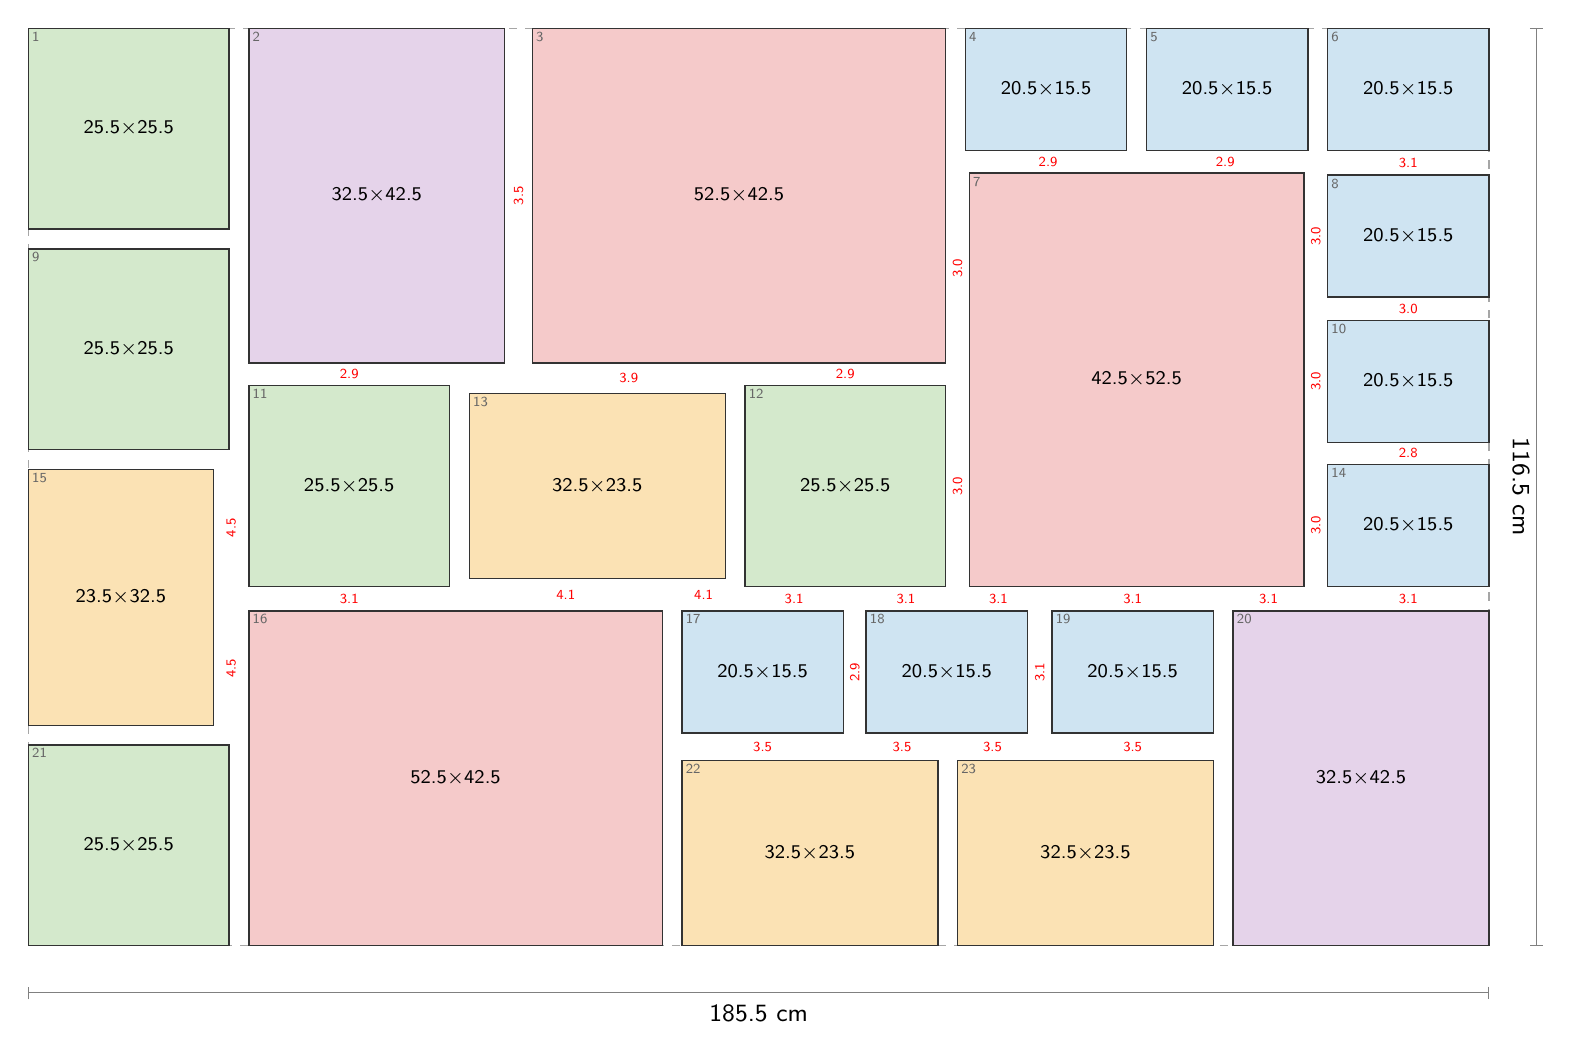
\begin{tikzpicture}[x=1mm, y=-1mm]
\draw[gray!70, dashed, line width=0.4pt] (0,0) rectangle (185.50,116.50);
\filldraw[fill=ft2, draw=black!80, line width=0.5pt] (0.00,0.00) rectangle (25.50,25.50);
\node[align=center, inner sep=0pt] at (12.75,12.75) {\scriptsize 25.5$\times$25.5};
\node[anchor=north west, inner sep=1.2pt, font=\tiny, text=black!60] at (0.00,0.00) {1};
\filldraw[fill=ft3, draw=black!80, line width=0.5pt] (28.00,0.00) rectangle (60.50,42.50);
\node[align=center, inner sep=0pt] at (44.25,21.25) {\scriptsize 32.5$\times$42.5};
\node[anchor=north west, inner sep=1.2pt, font=\tiny, text=black!60] at (28.00,0.00) {2};
\filldraw[fill=ft4, draw=black!80, line width=0.5pt] (64.00,0.00) rectangle (116.50,42.50);
\node[align=center, inner sep=0pt] at (90.25,21.25) {\scriptsize 52.5$\times$42.5};
\node[anchor=north west, inner sep=1.2pt, font=\tiny, text=black!60] at (64.00,0.00) {3};
\filldraw[fill=ft0, draw=black!80, line width=0.5pt] (119.00,0.00) rectangle (139.50,15.50);
\node[align=center, inner sep=0pt] at (129.25,7.75) {\scriptsize 20.5$\times$15.5};
\node[anchor=north west, inner sep=1.2pt, font=\tiny, text=black!60] at (119.00,0.00) {4};
\filldraw[fill=ft0, draw=black!80, line width=0.5pt] (142.00,0.00) rectangle (162.50,15.50);
\node[align=center, inner sep=0pt] at (152.25,7.75) {\scriptsize 20.5$\times$15.5};
\node[anchor=north west, inner sep=1.2pt, font=\tiny, text=black!60] at (142.00,0.00) {5};
\filldraw[fill=ft0, draw=black!80, line width=0.5pt] (165.00,0.00) rectangle (185.50,15.50);
\node[align=center, inner sep=0pt] at (175.25,7.75) {\scriptsize 20.5$\times$15.5};
\node[anchor=north west, inner sep=1.2pt, font=\tiny, text=black!60] at (165.00,0.00) {6};
\filldraw[fill=ft4, draw=black!80, line width=0.5pt] (119.50,18.38) rectangle (162.00,70.88);
\node[align=center, inner sep=0pt] at (140.75,44.63) {\scriptsize 42.5$\times$52.5};
\node[anchor=north west, inner sep=1.2pt, font=\tiny, text=black!60] at (119.50,18.38) {7};
\filldraw[fill=ft0, draw=black!80, line width=0.5pt] (165.00,18.63) rectangle (185.50,34.13);
\node[align=center, inner sep=0pt] at (175.25,26.38) {\scriptsize 20.5$\times$15.5};
\node[anchor=north west, inner sep=1.2pt, font=\tiny, text=black!60] at (165.00,18.63) {8};
\filldraw[fill=ft2, draw=black!80, line width=0.5pt] (0.00,28.00) rectangle (25.50,53.50);
\node[align=center, inner sep=0pt] at (12.75,40.75) {\scriptsize 25.5$\times$25.5};
\node[anchor=north west, inner sep=1.2pt, font=\tiny, text=black!60] at (0.00,28.00) {9};
\filldraw[fill=ft0, draw=black!80, line width=0.5pt] (165.00,37.09) rectangle (185.50,52.59);
\node[align=center, inner sep=0pt] at (175.25,44.84) {\scriptsize 20.5$\times$15.5};
\node[anchor=north west, inner sep=1.2pt, font=\tiny, text=black!60] at (165.00,37.09) {10};
\filldraw[fill=ft2, draw=black!80, line width=0.5pt] (28.00,45.38) rectangle (53.50,70.88);
\node[align=center, inner sep=0pt] at (40.75,58.13) {\scriptsize 25.5$\times$25.5};
\node[anchor=north west, inner sep=1.2pt, font=\tiny, text=black!60] at (28.00,45.38) {11};
\filldraw[fill=ft2, draw=black!80, line width=0.5pt] (91.00,45.38) rectangle (116.50,70.88);
\node[align=center, inner sep=0pt] at (103.75,58.13) {\scriptsize 25.5$\times$25.5};
\node[anchor=north west, inner sep=1.2pt, font=\tiny, text=black!60] at (91.00,45.38) {12};
\filldraw[fill=ft1, draw=black!80, line width=0.5pt] (56.00,46.38) rectangle (88.50,69.88);
\node[align=center, inner sep=0pt] at (72.25,58.13) {\scriptsize 32.5$\times$23.5};
\node[anchor=north west, inner sep=1.2pt, font=\tiny, text=black!60] at (56.00,46.38) {13};
\filldraw[fill=ft0, draw=black!80, line width=0.5pt] (165.00,55.38) rectangle (185.50,70.88);
\node[align=center, inner sep=0pt] at (175.25,63.13) {\scriptsize 20.5$\times$15.5};
\node[anchor=north west, inner sep=1.2pt, font=\tiny, text=black!60] at (165.00,55.38) {14};
\filldraw[fill=ft1, draw=black!80, line width=0.5pt] (0.00,56.00) rectangle (23.50,88.50);
\node[align=center, inner sep=0pt] at (11.75,72.25) {\scriptsize 23.5$\times$32.5};
\node[anchor=north west, inner sep=1.2pt, font=\tiny, text=black!60] at (0.00,56.00) {15};
\filldraw[fill=ft4, draw=black!80, line width=0.5pt] (28.00,74.00) rectangle (80.50,116.50);
\node[align=center, inner sep=0pt] at (54.25,95.25) {\scriptsize 52.5$\times$42.5};
\node[anchor=north west, inner sep=1.2pt, font=\tiny, text=black!60] at (28.00,74.00) {16};
\filldraw[fill=ft0, draw=black!80, line width=0.5pt] (83.00,74.00) rectangle (103.50,89.50);
\node[align=center, inner sep=0pt] at (93.25,81.75) {\scriptsize 20.5$\times$15.5};
\node[anchor=north west, inner sep=1.2pt, font=\tiny, text=black!60] at (83.00,74.00) {17};
\filldraw[fill=ft0, draw=black!80, line width=0.5pt] (106.39,74.00) rectangle (126.89,89.50);
\node[align=center, inner sep=0pt] at (116.64,81.75) {\scriptsize 20.5$\times$15.5};
\node[anchor=north west, inner sep=1.2pt, font=\tiny, text=black!60] at (106.39,74.00) {18};
\filldraw[fill=ft0, draw=black!80, line width=0.5pt] (130.00,74.00) rectangle (150.50,89.50);
\node[align=center, inner sep=0pt] at (140.25,81.75) {\scriptsize 20.5$\times$15.5};
\node[anchor=north west, inner sep=1.2pt, font=\tiny, text=black!60] at (130.00,74.00) {19};
\filldraw[fill=ft3, draw=black!80, line width=0.5pt] (153.00,74.00) rectangle (185.50,116.50);
\node[align=center, inner sep=0pt] at (169.25,95.25) {\scriptsize 32.5$\times$42.5};
\node[anchor=north west, inner sep=1.2pt, font=\tiny, text=black!60] at (153.00,74.00) {20};
\filldraw[fill=ft2, draw=black!80, line width=0.5pt] (0.00,91.00) rectangle (25.50,116.50);
\node[align=center, inner sep=0pt] at (12.75,103.75) {\scriptsize 25.5$\times$25.5};
\node[anchor=north west, inner sep=1.2pt, font=\tiny, text=black!60] at (0.00,91.00) {21};
\filldraw[fill=ft1, draw=black!80, line width=0.5pt] (83.00,93.00) rectangle (115.50,116.50);
\node[align=center, inner sep=0pt] at (99.25,104.75) {\scriptsize 32.5$\times$23.5};
\node[anchor=north west, inner sep=1.2pt, font=\tiny, text=black!60] at (83.00,93.00) {22};
\filldraw[fill=ft1, draw=black!80, line width=0.5pt] (118.00,93.00) rectangle (150.50,116.50);
\node[align=center, inner sep=0pt] at (134.25,104.75) {\scriptsize 32.5$\times$23.5};
\node[anchor=north west, inner sep=1.2pt, font=\tiny, text=black!60] at (118.00,93.00) {23};
\node[font=\tiny, text=red, fill=white, inner sep=0.3pt, rotate=90] at (62.25,21.25) {3.5};
\node[font=\tiny, text=red, fill=white, inner sep=0.3pt] at (40.75,43.94) {2.9};
\node[font=\tiny, text=red, fill=white, inner sep=0.3pt, rotate=90] at (118.00,30.44) {3.0};
\node[font=\tiny, text=red, fill=white, inner sep=0.3pt] at (103.75,43.94) {2.9};
\node[font=\tiny, text=red, fill=white, inner sep=0.3pt] at (76.25,44.44) {3.9};
\node[font=\tiny, text=red, fill=white, inner sep=0.3pt] at (129.50,16.94) {2.9};
\node[font=\tiny, text=red, fill=white, inner sep=0.3pt] at (152.00,16.94) {2.9};
\node[font=\tiny, text=red, fill=white, inner sep=0.3pt] at (175.25,17.06) {3.1};
\node[font=\tiny, text=red, fill=white, inner sep=0.3pt, rotate=90] at (163.50,26.38) {3.0};
\node[font=\tiny, text=red, fill=white, inner sep=0.3pt, rotate=90] at (163.50,44.84) {3.0};
\node[font=\tiny, text=red, fill=white, inner sep=0.3pt, rotate=90] at (163.50,63.13) {3.0};
\node[font=\tiny, text=red, fill=white, inner sep=0.3pt] at (123.20,72.44) {3.1};
\node[font=\tiny, text=red, fill=white, inner sep=0.3pt] at (140.25,72.44) {3.1};
\node[font=\tiny, text=red, fill=white, inner sep=0.3pt] at (157.50,72.44) {3.1};
\node[font=\tiny, text=red, fill=white, inner sep=0.3pt] at (175.25,35.61) {3.0};
\node[font=\tiny, text=red, fill=white, inner sep=0.3pt] at (175.25,53.98) {2.8};
\node[font=\tiny, text=red, fill=white, inner sep=0.3pt] at (40.75,72.44) {3.1};
\node[font=\tiny, text=red, fill=white, inner sep=0.3pt, rotate=90] at (118.00,58.13) {3.0};
\node[font=\tiny, text=red, fill=white, inner sep=0.3pt] at (97.25,72.44) {3.1};
\node[font=\tiny, text=red, fill=white, inner sep=0.3pt] at (111.45,72.44) {3.1};
\node[font=\tiny, text=red, fill=white, inner sep=0.3pt] at (68.25,71.94) {4.1};
\node[font=\tiny, text=red, fill=white, inner sep=0.3pt] at (85.75,71.94) {4.1};
\node[font=\tiny, text=red, fill=white, inner sep=0.3pt] at (175.25,72.44) {3.1};
\node[font=\tiny, text=red, fill=white, inner sep=0.3pt, rotate=90] at (25.75,63.44) {4.5};
\node[font=\tiny, text=red, fill=white, inner sep=0.3pt, rotate=90] at (25.75,81.25) {4.5};
\node[font=\tiny, text=red, fill=white, inner sep=0.3pt, rotate=90] at (104.95,81.75) {2.9};
\node[font=\tiny, text=red, fill=white, inner sep=0.3pt] at (93.25,91.25) {3.5};
\node[font=\tiny, text=red, fill=white, inner sep=0.3pt, rotate=90] at (128.45,81.75) {3.1};
\node[font=\tiny, text=red, fill=white, inner sep=0.3pt] at (110.95,91.25) {3.5};
\node[font=\tiny, text=red, fill=white, inner sep=0.3pt] at (122.45,91.25) {3.5};
\node[font=\tiny, text=red, fill=white, inner sep=0.3pt] at (140.25,91.25) {3.5};
\draw[Bar-Bar, gray] (0,122.50) -- (185.50,122.50) node[midway, below=1pt, font=\small, text=black] {185.5 cm};
\draw[Bar-Bar, gray] (191.50,0) -- (191.50,116.50) node[midway, right=1pt, font=\small, text=black, rotate=-90, anchor=north] {116.5 cm};
\end{tikzpicture}\\[4pt]
{\scriptsize Scale 1:10 (1 mm = 1 cm). Red numbers mark gaps that deviate from the nominal gap by more than 0.25 cm. Small grey numbers index the coordinate table.}
\end{minipage}\hfill
\begin{minipage}[t]{0.25\textwidth}\vspace{0pt}
\small
\begin{tabular}{@{}l l@{}}
\toprule
Outer size & 185.5 $\times$ 116.5 cm \\
Nominal gap & 2.5 cm \\
Actual gaps & 2.5 -- 4.5 cm \\
Max.\ deviation & 2.0 cm \\
Mean deviation & 0.51 cm \\
Border notches & none \\
Corners filled & 4 / 4 \\
Frames used & 23 of 28 \\
Large frames & {\scriptsize 3, touching 1$\times$ (24 cm), min.\ dist.\ 56 cm} \\
Entropy & 0.77 \\
\quad {\scriptsize mix / variety} & {\scriptsize 0.76 / 0.77} \\
\quad {\scriptsize stagger / lines} & {\scriptsize 0.57 / 1.00 (1 through)} \\
\bottomrule
\end{tabular}

\vspace{8pt}
\scriptsize
\begin{tabular}{@{}c l l r r@{}}
\toprule
 & outer w $\times$ h (cm) &  & used & have \\
\midrule
\tikz[baseline=-0.6ex]\fill[ft0,draw=black!60] (0,0) rectangle (1.2ex,1.2ex); & 20.5$\times$15.5 & L & 9 & 9 \\
\tikz[baseline=-0.6ex]\fill[ft0,draw=black!60] (0,0) rectangle (1.2ex,1.2ex); & 15.5$\times$20.5 & P & 0 & 2 \\
\tikz[baseline=-0.6ex]\fill[ft3,draw=black!60] (0,0) rectangle (1.2ex,1.2ex); & 32.5$\times$42.5 & P & 2 & 2 \\
\tikz[baseline=-0.6ex]\fill[ft3,draw=black!60] (0,0) rectangle (1.2ex,1.2ex); & 42.5$\times$32.5 & L & 0 & 1 \\
\tikz[baseline=-0.6ex]\fill[ft1,draw=black!60] (0,0) rectangle (1.2ex,1.2ex); & 32.5$\times$23.5 & L & 3 & 5 \\
\tikz[baseline=-0.6ex]\fill[ft1,draw=black!60] (0,0) rectangle (1.2ex,1.2ex); & 23.5$\times$32.5 & P & 1 & 1 \\
\tikz[baseline=-0.6ex]\fill[ft2,draw=black!60] (0,0) rectangle (1.2ex,1.2ex); & 25.5$\times$25.5 &  & 5 & 5 \\
\tikz[baseline=-0.6ex]\fill[ft4,draw=black!60] (0,0) rectangle (1.2ex,1.2ex); & 42.5$\times$52.5 & P & 1 & 1 \\
\tikz[baseline=-0.6ex]\fill[ft4,draw=black!60] (0,0) rectangle (1.2ex,1.2ex); & 52.5$\times$42.5 & L & 2 & 2 \\
\bottomrule
\end{tabular}

\vspace{8pt}
{\bfseries Positions} (top-left corner, cm)\\[2pt]
\tiny
\begin{tabular}{@{}r l r r@{}}
\toprule
\# & frame w $\times$ h & x & y \\
\midrule
1 & 25.5 $\times$ 25.5 & 0.0 & 0.0 \\
2 & 32.5 $\times$ 42.5 & 28.0 & 0.0 \\
3 & 52.5 $\times$ 42.5 & 64.0 & 0.0 \\
4 & 20.5 $\times$ 15.5 & 119.0 & 0.0 \\
5 & 20.5 $\times$ 15.5 & 142.0 & 0.0 \\
6 & 20.5 $\times$ 15.5 & 165.0 & 0.0 \\
7 & 42.5 $\times$ 52.5 & 119.5 & 18.4 \\
8 & 20.5 $\times$ 15.5 & 165.0 & 18.6 \\
9 & 25.5 $\times$ 25.5 & 0.0 & 28.0 \\
10 & 20.5 $\times$ 15.5 & 165.0 & 37.1 \\
11 & 25.5 $\times$ 25.5 & 28.0 & 45.4 \\
12 & 25.5 $\times$ 25.5 & 91.0 & 45.4 \\
13 & 32.5 $\times$ 23.5 & 56.0 & 46.4 \\
14 & 20.5 $\times$ 15.5 & 165.0 & 55.4 \\
15 & 23.5 $\times$ 32.5 & 0.0 & 56.0 \\
16 & 52.5 $\times$ 42.5 & 28.0 & 74.0 \\
17 & 20.5 $\times$ 15.5 & 83.0 & 74.0 \\
18 & 20.5 $\times$ 15.5 & 106.4 & 74.0 \\
19 & 20.5 $\times$ 15.5 & 130.0 & 74.0 \\
20 & 32.5 $\times$ 42.5 & 153.0 & 74.0 \\
21 & 25.5 $\times$ 25.5 & 0.0 & 91.0 \\
22 & 32.5 $\times$ 23.5 & 83.0 & 93.0 \\
23 & 32.5 $\times$ 23.5 & 118.0 & 93.0 \\
\bottomrule
\end{tabular}
\end{minipage}
\clearpage

\phantomsection\addcontentsline{toc}{subsection}{Layout 2: 184.0 \texorpdfstring{$\times$}{x} 115.0 cm, 23 frames, gap 2 cm, max.\ deviation 2.0 cm}
\label{lay:proportional:2}
\begin{minipage}[t]{0.74\textwidth}\vspace{0pt}
{\LARGE\bfseries Layout 2}\hspace{1.5em}{\large 184.0 $\times$ 115.0 cm \quad gap 2 cm \quad 23 frames}\\[8pt]
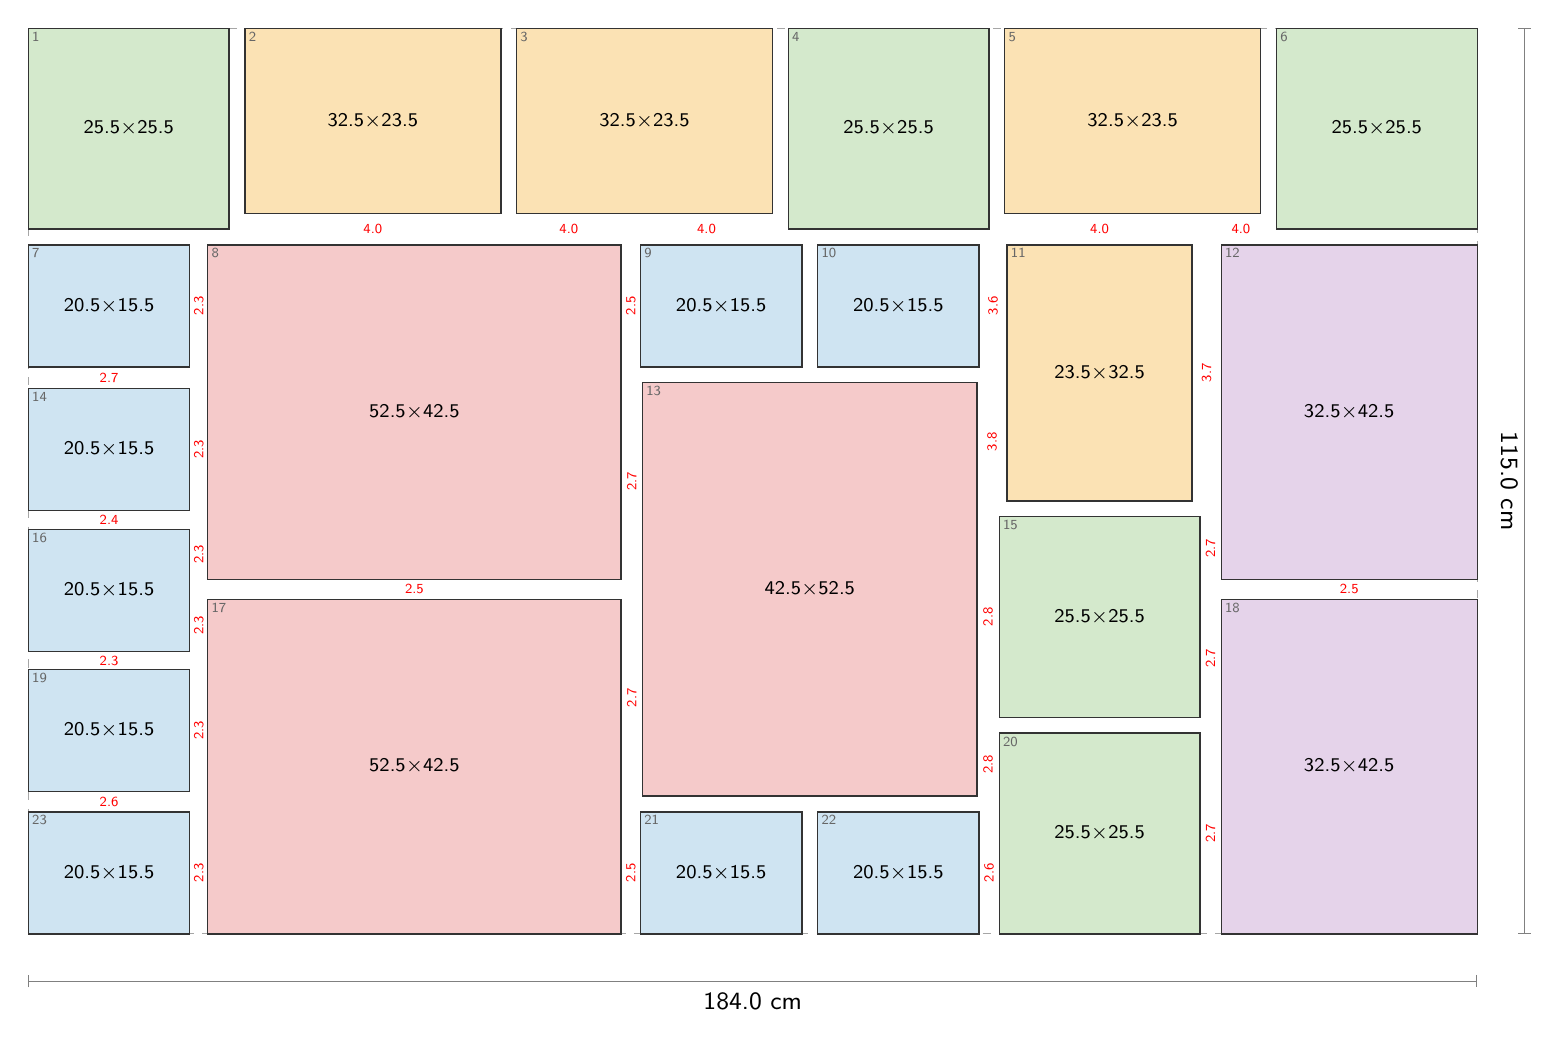
\begin{tikzpicture}[x=1mm, y=-1mm]
\draw[gray!70, dashed, line width=0.4pt] (0,0) rectangle (184.00,115.00);
\filldraw[fill=ft2, draw=black!80, line width=0.5pt] (0.00,0.00) rectangle (25.50,25.50);
\node[align=center, inner sep=0pt] at (12.75,12.75) {\scriptsize 25.5$\times$25.5};
\node[anchor=north west, inner sep=1.2pt, font=\tiny, text=black!60] at (0.00,0.00) {1};
\filldraw[fill=ft1, draw=black!80, line width=0.5pt] (27.50,0.00) rectangle (60.00,23.50);
\node[align=center, inner sep=0pt] at (43.75,11.75) {\scriptsize 32.5$\times$23.5};
\node[anchor=north west, inner sep=1.2pt, font=\tiny, text=black!60] at (27.50,0.00) {2};
\filldraw[fill=ft1, draw=black!80, line width=0.5pt] (62.00,0.00) rectangle (94.50,23.50);
\node[align=center, inner sep=0pt] at (78.25,11.75) {\scriptsize 32.5$\times$23.5};
\node[anchor=north west, inner sep=1.2pt, font=\tiny, text=black!60] at (62.00,0.00) {3};
\filldraw[fill=ft2, draw=black!80, line width=0.5pt] (96.50,0.00) rectangle (122.00,25.50);
\node[align=center, inner sep=0pt] at (109.25,12.75) {\scriptsize 25.5$\times$25.5};
\node[anchor=north west, inner sep=1.2pt, font=\tiny, text=black!60] at (96.50,0.00) {4};
\filldraw[fill=ft1, draw=black!80, line width=0.5pt] (124.00,0.00) rectangle (156.50,23.50);
\node[align=center, inner sep=0pt] at (140.25,11.75) {\scriptsize 32.5$\times$23.5};
\node[anchor=north west, inner sep=1.2pt, font=\tiny, text=black!60] at (124.00,0.00) {5};
\filldraw[fill=ft2, draw=black!80, line width=0.5pt] (158.50,0.00) rectangle (184.00,25.50);
\node[align=center, inner sep=0pt] at (171.25,12.75) {\scriptsize 25.5$\times$25.5};
\node[anchor=north west, inner sep=1.2pt, font=\tiny, text=black!60] at (158.50,0.00) {6};
\filldraw[fill=ft0, draw=black!80, line width=0.5pt] (0.00,27.50) rectangle (20.50,43.00);
\node[align=center, inner sep=0pt] at (10.25,35.25) {\scriptsize 20.5$\times$15.5};
\node[anchor=north west, inner sep=1.2pt, font=\tiny, text=black!60] at (0.00,27.50) {7};
\filldraw[fill=ft4, draw=black!80, line width=0.5pt] (22.78,27.50) rectangle (75.28,70.00);
\node[align=center, inner sep=0pt] at (49.03,48.75) {\scriptsize 52.5$\times$42.5};
\node[anchor=north west, inner sep=1.2pt, font=\tiny, text=black!60] at (22.78,27.50) {8};
\filldraw[fill=ft0, draw=black!80, line width=0.5pt] (77.74,27.50) rectangle (98.24,43.00);
\node[align=center, inner sep=0pt] at (87.99,35.25) {\scriptsize 20.5$\times$15.5};
\node[anchor=north west, inner sep=1.2pt, font=\tiny, text=black!60] at (77.74,27.50) {9};
\filldraw[fill=ft0, draw=black!80, line width=0.5pt] (100.24,27.50) rectangle (120.74,43.00);
\node[align=center, inner sep=0pt] at (110.49,35.25) {\scriptsize 20.5$\times$15.5};
\node[anchor=north west, inner sep=1.2pt, font=\tiny, text=black!60] at (100.24,27.50) {10};
\filldraw[fill=ft1, draw=black!80, line width=0.5pt] (124.30,27.50) rectangle (147.80,60.00);
\node[align=center, inner sep=0pt] at (136.05,43.75) {\scriptsize 23.5$\times$32.5};
\node[anchor=north west, inner sep=1.2pt, font=\tiny, text=black!60] at (124.30,27.50) {11};
\filldraw[fill=ft3, draw=black!80, line width=0.5pt] (151.50,27.50) rectangle (184.00,70.00);
\node[align=center, inner sep=0pt] at (167.75,48.75) {\scriptsize 32.5$\times$42.5};
\node[anchor=north west, inner sep=1.2pt, font=\tiny, text=black!60] at (151.50,27.50) {12};
\filldraw[fill=ft4, draw=black!80, line width=0.5pt] (77.99,45.00) rectangle (120.49,97.50);
\node[align=center, inner sep=0pt] at (99.24,71.25) {\scriptsize 42.5$\times$52.5};
\node[anchor=north west, inner sep=1.2pt, font=\tiny, text=black!60] at (77.99,45.00) {13};
\filldraw[fill=ft0, draw=black!80, line width=0.5pt] (0.00,45.73) rectangle (20.50,61.23);
\node[align=center, inner sep=0pt] at (10.25,53.48) {\scriptsize 20.5$\times$15.5};
\node[anchor=north west, inner sep=1.2pt, font=\tiny, text=black!60] at (0.00,45.73) {14};
\filldraw[fill=ft2, draw=black!80, line width=0.5pt] (123.30,62.00) rectangle (148.80,87.50);
\node[align=center, inner sep=0pt] at (136.05,74.75) {\scriptsize 25.5$\times$25.5};
\node[anchor=north west, inner sep=1.2pt, font=\tiny, text=black!60] at (123.30,62.00) {15};
\filldraw[fill=ft0, draw=black!80, line width=0.5pt] (0.00,63.65) rectangle (20.50,79.15);
\node[align=center, inner sep=0pt] at (10.25,71.40) {\scriptsize 20.5$\times$15.5};
\node[anchor=north west, inner sep=1.2pt, font=\tiny, text=black!60] at (0.00,63.65) {16};
\filldraw[fill=ft4, draw=black!80, line width=0.5pt] (22.78,72.50) rectangle (75.28,115.00);
\node[align=center, inner sep=0pt] at (49.03,93.75) {\scriptsize 52.5$\times$42.5};
\node[anchor=north west, inner sep=1.2pt, font=\tiny, text=black!60] at (22.78,72.50) {17};
\filldraw[fill=ft3, draw=black!80, line width=0.5pt] (151.50,72.50) rectangle (184.00,115.00);
\node[align=center, inner sep=0pt] at (167.75,93.75) {\scriptsize 32.5$\times$42.5};
\node[anchor=north west, inner sep=1.2pt, font=\tiny, text=black!60] at (151.50,72.50) {18};
\filldraw[fill=ft0, draw=black!80, line width=0.5pt] (0.00,81.42) rectangle (20.50,96.92);
\node[align=center, inner sep=0pt] at (10.25,89.17) {\scriptsize 20.5$\times$15.5};
\node[anchor=north west, inner sep=1.2pt, font=\tiny, text=black!60] at (0.00,81.42) {19};
\filldraw[fill=ft2, draw=black!80, line width=0.5pt] (123.30,89.50) rectangle (148.80,115.00);
\node[align=center, inner sep=0pt] at (136.05,102.25) {\scriptsize 25.5$\times$25.5};
\node[anchor=north west, inner sep=1.2pt, font=\tiny, text=black!60] at (123.30,89.50) {20};
\filldraw[fill=ft0, draw=black!80, line width=0.5pt] (77.74,99.50) rectangle (98.24,115.00);
\node[align=center, inner sep=0pt] at (87.99,107.25) {\scriptsize 20.5$\times$15.5};
\node[anchor=north west, inner sep=1.2pt, font=\tiny, text=black!60] at (77.74,99.50) {21};
\filldraw[fill=ft0, draw=black!80, line width=0.5pt] (100.24,99.50) rectangle (120.74,115.00);
\node[align=center, inner sep=0pt] at (110.49,107.25) {\scriptsize 20.5$\times$15.5};
\node[anchor=north west, inner sep=1.2pt, font=\tiny, text=black!60] at (100.24,99.50) {22};
\filldraw[fill=ft0, draw=black!80, line width=0.5pt] (0.00,99.50) rectangle (20.50,115.00);
\node[align=center, inner sep=0pt] at (10.25,107.25) {\scriptsize 20.5$\times$15.5};
\node[anchor=north west, inner sep=1.2pt, font=\tiny, text=black!60] at (0.00,99.50) {23};
\node[font=\tiny, text=red, fill=white, inner sep=0.3pt] at (43.75,25.50) {4.0};
\node[font=\tiny, text=red, fill=white, inner sep=0.3pt] at (68.64,25.50) {4.0};
\node[font=\tiny, text=red, fill=white, inner sep=0.3pt] at (86.12,25.50) {4.0};
\node[font=\tiny, text=red, fill=white, inner sep=0.3pt] at (136.05,25.50) {4.0};
\node[font=\tiny, text=red, fill=white, inner sep=0.3pt] at (154.00,25.50) {4.0};
\node[font=\tiny, text=red, fill=white, inner sep=0.3pt, rotate=90] at (21.64,35.25) {2.3};
\node[font=\tiny, text=red, fill=white, inner sep=0.3pt] at (10.25,44.36) {2.7};
\node[font=\tiny, text=red, fill=white, inner sep=0.3pt, rotate=90] at (76.51,35.25) {2.5};
\node[font=\tiny, text=red, fill=white, inner sep=0.3pt, rotate=90] at (76.64,57.50) {2.7};
\node[font=\tiny, text=red, fill=white, inner sep=0.3pt] at (49.03,71.25) {2.5};
\node[font=\tiny, text=red, fill=white, inner sep=0.3pt, rotate=90] at (122.52,35.25) {3.6};
\node[font=\tiny, text=red, fill=white, inner sep=0.3pt, rotate=90] at (149.65,43.75) {3.7};
\node[font=\tiny, text=red, fill=white, inner sep=0.3pt] at (167.75,71.25) {2.5};
\node[font=\tiny, text=red, fill=white, inner sep=0.3pt, rotate=90] at (122.40,52.50) {3.8};
\node[font=\tiny, text=red, fill=white, inner sep=0.3pt, rotate=90] at (121.90,74.75) {2.8};
\node[font=\tiny, text=red, fill=white, inner sep=0.3pt, rotate=90] at (121.90,93.50) {2.8};
\node[font=\tiny, text=red, fill=white, inner sep=0.3pt, rotate=90] at (21.64,53.48) {2.3};
\node[font=\tiny, text=red, fill=white, inner sep=0.3pt] at (10.25,62.44) {2.4};
\node[font=\tiny, text=red, fill=white, inner sep=0.3pt, rotate=90] at (150.15,66.00) {2.7};
\node[font=\tiny, text=red, fill=white, inner sep=0.3pt, rotate=90] at (150.15,80.00) {2.7};
\node[font=\tiny, text=red, fill=white, inner sep=0.3pt, rotate=90] at (21.64,66.83) {2.3};
\node[font=\tiny, text=red, fill=white, inner sep=0.3pt, rotate=90] at (21.64,75.83) {2.3};
\node[font=\tiny, text=red, fill=white, inner sep=0.3pt] at (10.25,80.29) {2.3};
\node[font=\tiny, text=red, fill=white, inner sep=0.3pt, rotate=90] at (76.64,85.00) {2.7};
\node[font=\tiny, text=red, fill=white, inner sep=0.3pt, rotate=90] at (76.51,107.25) {2.5};
\node[font=\tiny, text=red, fill=white, inner sep=0.3pt, rotate=90] at (21.64,89.17) {2.3};
\node[font=\tiny, text=red, fill=white, inner sep=0.3pt] at (10.25,98.21) {2.6};
\node[font=\tiny, text=red, fill=white, inner sep=0.3pt, rotate=90] at (150.15,102.25) {2.7};
\node[font=\tiny, text=red, fill=white, inner sep=0.3pt, rotate=90] at (122.02,107.25) {2.6};
\node[font=\tiny, text=red, fill=white, inner sep=0.3pt, rotate=90] at (21.64,107.25) {2.3};
\draw[Bar-Bar, gray] (0,121.00) -- (184.00,121.00) node[midway, below=1pt, font=\small, text=black] {184.0 cm};
\draw[Bar-Bar, gray] (190.00,0) -- (190.00,115.00) node[midway, right=1pt, font=\small, text=black, rotate=-90, anchor=north] {115.0 cm};
\end{tikzpicture}\\[4pt]
{\scriptsize Scale 1:10 (1 mm = 1 cm). Red numbers mark gaps that deviate from the nominal gap by more than 0.25 cm. Small grey numbers index the coordinate table.}
\end{minipage}\hfill
\begin{minipage}[t]{0.25\textwidth}\vspace{0pt}
\small
\begin{tabular}{@{}l l@{}}
\toprule
Outer size & 184.0 $\times$ 115.0 cm \\
Nominal gap & 2 cm \\
Actual gaps & 2.0 -- 4.0 cm \\
Max.\ deviation & 2.0 cm \\
Mean deviation & 0.57 cm \\
Border notches & none \\
Corners filled & 4 / 4 \\
Frames used & 23 of 28 \\
Large frames & {\scriptsize 3, touching 3$\times$ (102 cm), min.\ dist.\ 45 cm} \\
Entropy & 0.69 \\
\quad {\scriptsize mix / variety} & {\scriptsize 0.76 / 0.74} \\
\quad {\scriptsize stagger / lines} & {\scriptsize 0.51 / 0.75 (2 through)} \\
\bottomrule
\end{tabular}

\vspace{8pt}
\scriptsize
\begin{tabular}{@{}c l l r r@{}}
\toprule
 & outer w $\times$ h (cm) &  & used & have \\
\midrule
\tikz[baseline=-0.6ex]\fill[ft0,draw=black!60] (0,0) rectangle (1.2ex,1.2ex); & 20.5$\times$15.5 & L & 9 & 9 \\
\tikz[baseline=-0.6ex]\fill[ft0,draw=black!60] (0,0) rectangle (1.2ex,1.2ex); & 15.5$\times$20.5 & P & 0 & 2 \\
\tikz[baseline=-0.6ex]\fill[ft3,draw=black!60] (0,0) rectangle (1.2ex,1.2ex); & 32.5$\times$42.5 & P & 2 & 2 \\
\tikz[baseline=-0.6ex]\fill[ft3,draw=black!60] (0,0) rectangle (1.2ex,1.2ex); & 42.5$\times$32.5 & L & 0 & 1 \\
\tikz[baseline=-0.6ex]\fill[ft1,draw=black!60] (0,0) rectangle (1.2ex,1.2ex); & 32.5$\times$23.5 & L & 3 & 5 \\
\tikz[baseline=-0.6ex]\fill[ft1,draw=black!60] (0,0) rectangle (1.2ex,1.2ex); & 23.5$\times$32.5 & P & 1 & 1 \\
\tikz[baseline=-0.6ex]\fill[ft2,draw=black!60] (0,0) rectangle (1.2ex,1.2ex); & 25.5$\times$25.5 &  & 5 & 5 \\
\tikz[baseline=-0.6ex]\fill[ft4,draw=black!60] (0,0) rectangle (1.2ex,1.2ex); & 42.5$\times$52.5 & P & 1 & 1 \\
\tikz[baseline=-0.6ex]\fill[ft4,draw=black!60] (0,0) rectangle (1.2ex,1.2ex); & 52.5$\times$42.5 & L & 2 & 2 \\
\bottomrule
\end{tabular}

\vspace{8pt}
{\bfseries Positions} (top-left corner, cm)\\[2pt]
\tiny
\begin{tabular}{@{}r l r r@{}}
\toprule
\# & frame w $\times$ h & x & y \\
\midrule
1 & 25.5 $\times$ 25.5 & 0.0 & 0.0 \\
2 & 32.5 $\times$ 23.5 & 27.5 & 0.0 \\
3 & 32.5 $\times$ 23.5 & 62.0 & 0.0 \\
4 & 25.5 $\times$ 25.5 & 96.5 & 0.0 \\
5 & 32.5 $\times$ 23.5 & 124.0 & 0.0 \\
6 & 25.5 $\times$ 25.5 & 158.5 & 0.0 \\
7 & 20.5 $\times$ 15.5 & 0.0 & 27.5 \\
8 & 52.5 $\times$ 42.5 & 22.8 & 27.5 \\
9 & 20.5 $\times$ 15.5 & 77.7 & 27.5 \\
10 & 20.5 $\times$ 15.5 & 100.2 & 27.5 \\
11 & 23.5 $\times$ 32.5 & 124.3 & 27.5 \\
12 & 32.5 $\times$ 42.5 & 151.5 & 27.5 \\
13 & 42.5 $\times$ 52.5 & 78.0 & 45.0 \\
14 & 20.5 $\times$ 15.5 & 0.0 & 45.7 \\
15 & 25.5 $\times$ 25.5 & 123.3 & 62.0 \\
16 & 20.5 $\times$ 15.5 & 0.0 & 63.7 \\
17 & 52.5 $\times$ 42.5 & 22.8 & 72.5 \\
18 & 32.5 $\times$ 42.5 & 151.5 & 72.5 \\
19 & 20.5 $\times$ 15.5 & 0.0 & 81.4 \\
20 & 25.5 $\times$ 25.5 & 123.3 & 89.5 \\
21 & 20.5 $\times$ 15.5 & 77.7 & 99.5 \\
22 & 20.5 $\times$ 15.5 & 100.2 & 99.5 \\
23 & 20.5 $\times$ 15.5 & 0.0 & 99.5 \\
\bottomrule
\end{tabular}
\end{minipage}
\clearpage

\phantomsection\addcontentsline{toc}{subsection}{Layout 3: 191.5 \texorpdfstring{$\times$}{x} 113.5 cm, 26 frames, gap 1.5 cm, max.\ deviation 2.6 cm}
\label{lay:proportional:3}
\begin{minipage}[t]{0.74\textwidth}\vspace{0pt}
{\LARGE\bfseries Layout 3}\hspace{1.5em}{\large 191.5 $\times$ 113.5 cm \quad gap 1.5 cm \quad 26 frames}\\[8pt]
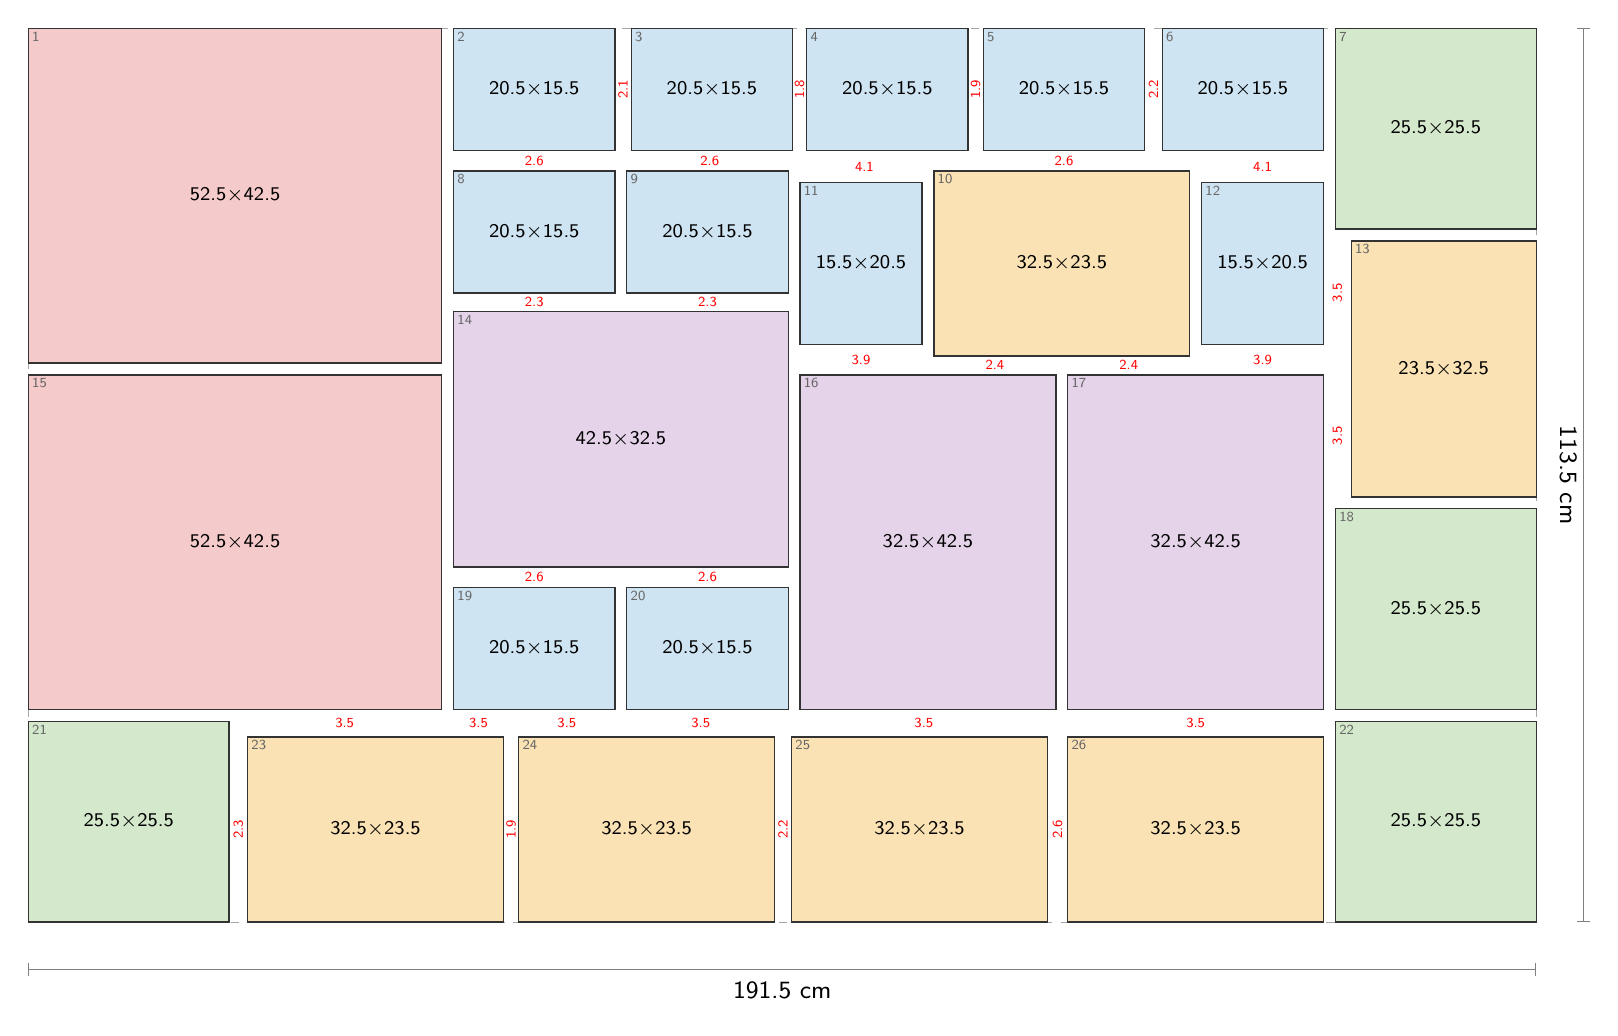
\begin{tikzpicture}[x=1mm, y=-1mm]
\draw[gray!70, dashed, line width=0.4pt] (0,0) rectangle (191.50,113.50);
\filldraw[fill=ft4, draw=black!80, line width=0.5pt] (0.00,0.00) rectangle (52.50,42.50);
\node[align=center, inner sep=0pt] at (26.25,21.25) {\scriptsize 52.5$\times$42.5};
\node[anchor=north west, inner sep=1.2pt, font=\tiny, text=black!60] at (0.00,0.00) {1};
\filldraw[fill=ft0, draw=black!80, line width=0.5pt] (54.00,0.00) rectangle (74.50,15.50);
\node[align=center, inner sep=0pt] at (64.25,7.75) {\scriptsize 20.5$\times$15.5};
\node[anchor=north west, inner sep=1.2pt, font=\tiny, text=black!60] at (54.00,0.00) {2};
\filldraw[fill=ft0, draw=black!80, line width=0.5pt] (76.57,0.00) rectangle (97.07,15.50);
\node[align=center, inner sep=0pt] at (86.82,7.75) {\scriptsize 20.5$\times$15.5};
\node[anchor=north west, inner sep=1.2pt, font=\tiny, text=black!60] at (76.57,0.00) {3};
\filldraw[fill=ft0, draw=black!80, line width=0.5pt] (98.85,0.00) rectangle (119.35,15.50);
\node[align=center, inner sep=0pt] at (109.10,7.75) {\scriptsize 20.5$\times$15.5};
\node[anchor=north west, inner sep=1.2pt, font=\tiny, text=black!60] at (98.85,0.00) {4};
\filldraw[fill=ft0, draw=black!80, line width=0.5pt] (121.28,0.00) rectangle (141.78,15.50);
\node[align=center, inner sep=0pt] at (131.53,7.75) {\scriptsize 20.5$\times$15.5};
\node[anchor=north west, inner sep=1.2pt, font=\tiny, text=black!60] at (121.28,0.00) {5};
\filldraw[fill=ft0, draw=black!80, line width=0.5pt] (144.00,0.00) rectangle (164.50,15.50);
\node[align=center, inner sep=0pt] at (154.25,7.75) {\scriptsize 20.5$\times$15.5};
\node[anchor=north west, inner sep=1.2pt, font=\tiny, text=black!60] at (144.00,0.00) {6};
\filldraw[fill=ft2, draw=black!80, line width=0.5pt] (166.00,0.00) rectangle (191.50,25.50);
\node[align=center, inner sep=0pt] at (178.75,12.75) {\scriptsize 25.5$\times$25.5};
\node[anchor=north west, inner sep=1.2pt, font=\tiny, text=black!60] at (166.00,0.00) {7};
\filldraw[fill=ft0, draw=black!80, line width=0.5pt] (54.00,18.11) rectangle (74.50,33.61);
\node[align=center, inner sep=0pt] at (64.25,25.86) {\scriptsize 20.5$\times$15.5};
\node[anchor=north west, inner sep=1.2pt, font=\tiny, text=black!60] at (54.00,18.11) {8};
\filldraw[fill=ft0, draw=black!80, line width=0.5pt] (76.00,18.11) rectangle (96.50,33.61);
\node[align=center, inner sep=0pt] at (86.25,25.86) {\scriptsize 20.5$\times$15.5};
\node[anchor=north west, inner sep=1.2pt, font=\tiny, text=black!60] at (76.00,18.11) {9};
\filldraw[fill=ft1, draw=black!80, line width=0.5pt] (115.00,18.11) rectangle (147.50,41.61);
\node[align=center, inner sep=0pt] at (131.25,29.86) {\scriptsize 32.5$\times$23.5};
\node[anchor=north west, inner sep=1.2pt, font=\tiny, text=black!60] at (115.00,18.11) {10};
\filldraw[fill=ft0, draw=black!80, line width=0.5pt] (98.00,19.61) rectangle (113.50,40.11);
\node[align=center, inner sep=0pt] at (105.75,29.86) {\scriptsize 15.5$\times$20.5};
\node[anchor=north west, inner sep=1.2pt, font=\tiny, text=black!60] at (98.00,19.61) {11};
\filldraw[fill=ft0, draw=black!80, line width=0.5pt] (149.00,19.61) rectangle (164.50,40.11);
\node[align=center, inner sep=0pt] at (156.75,29.86) {\scriptsize 15.5$\times$20.5};
\node[anchor=north west, inner sep=1.2pt, font=\tiny, text=black!60] at (149.00,19.61) {12};
\filldraw[fill=ft1, draw=black!80, line width=0.5pt] (168.00,27.00) rectangle (191.50,59.50);
\node[align=center, inner sep=0pt] at (179.75,43.25) {\scriptsize 23.5$\times$32.5};
\node[anchor=north west, inner sep=1.2pt, font=\tiny, text=black!60] at (168.00,27.00) {13};
\filldraw[fill=ft3, draw=black!80, line width=0.5pt] (54.00,35.92) rectangle (96.50,68.42);
\node[align=center, inner sep=0pt] at (75.25,52.17) {\scriptsize 42.5$\times$32.5};
\node[anchor=north west, inner sep=1.2pt, font=\tiny, text=black!60] at (54.00,35.92) {14};
\filldraw[fill=ft4, draw=black!80, line width=0.5pt] (0.00,44.00) rectangle (52.50,86.50);
\node[align=center, inner sep=0pt] at (26.25,65.25) {\scriptsize 52.5$\times$42.5};
\node[anchor=north west, inner sep=1.2pt, font=\tiny, text=black!60] at (0.00,44.00) {15};
\filldraw[fill=ft3, draw=black!80, line width=0.5pt] (98.00,44.00) rectangle (130.50,86.50);
\node[align=center, inner sep=0pt] at (114.25,65.25) {\scriptsize 32.5$\times$42.5};
\node[anchor=north west, inner sep=1.2pt, font=\tiny, text=black!60] at (98.00,44.00) {16};
\filldraw[fill=ft3, draw=black!80, line width=0.5pt] (132.00,44.00) rectangle (164.50,86.50);
\node[align=center, inner sep=0pt] at (148.25,65.25) {\scriptsize 32.5$\times$42.5};
\node[anchor=north west, inner sep=1.2pt, font=\tiny, text=black!60] at (132.00,44.00) {17};
\filldraw[fill=ft2, draw=black!80, line width=0.5pt] (166.00,61.00) rectangle (191.50,86.50);
\node[align=center, inner sep=0pt] at (178.75,73.75) {\scriptsize 25.5$\times$25.5};
\node[anchor=north west, inner sep=1.2pt, font=\tiny, text=black!60] at (166.00,61.00) {18};
\filldraw[fill=ft0, draw=black!80, line width=0.5pt] (54.00,71.00) rectangle (74.50,86.50);
\node[align=center, inner sep=0pt] at (64.25,78.75) {\scriptsize 20.5$\times$15.5};
\node[anchor=north west, inner sep=1.2pt, font=\tiny, text=black!60] at (54.00,71.00) {19};
\filldraw[fill=ft0, draw=black!80, line width=0.5pt] (76.00,71.00) rectangle (96.50,86.50);
\node[align=center, inner sep=0pt] at (86.25,78.75) {\scriptsize 20.5$\times$15.5};
\node[anchor=north west, inner sep=1.2pt, font=\tiny, text=black!60] at (76.00,71.00) {20};
\filldraw[fill=ft2, draw=black!80, line width=0.5pt] (0.00,88.00) rectangle (25.50,113.50);
\node[align=center, inner sep=0pt] at (12.75,100.75) {\scriptsize 25.5$\times$25.5};
\node[anchor=north west, inner sep=1.2pt, font=\tiny, text=black!60] at (0.00,88.00) {21};
\filldraw[fill=ft2, draw=black!80, line width=0.5pt] (166.00,88.00) rectangle (191.50,113.50);
\node[align=center, inner sep=0pt] at (178.75,100.75) {\scriptsize 25.5$\times$25.5};
\node[anchor=north west, inner sep=1.2pt, font=\tiny, text=black!60] at (166.00,88.00) {22};
\filldraw[fill=ft1, draw=black!80, line width=0.5pt] (27.84,90.00) rectangle (60.34,113.50);
\node[align=center, inner sep=0pt] at (44.09,101.75) {\scriptsize 32.5$\times$23.5};
\node[anchor=north west, inner sep=1.2pt, font=\tiny, text=black!60] at (27.84,90.00) {23};
\filldraw[fill=ft1, draw=black!80, line width=0.5pt] (62.27,90.00) rectangle (94.77,113.50);
\node[align=center, inner sep=0pt] at (78.52,101.75) {\scriptsize 32.5$\times$23.5};
\node[anchor=north west, inner sep=1.2pt, font=\tiny, text=black!60] at (62.27,90.00) {24};
\filldraw[fill=ft1, draw=black!80, line width=0.5pt] (96.93,90.00) rectangle (129.43,113.50);
\node[align=center, inner sep=0pt] at (113.18,101.75) {\scriptsize 32.5$\times$23.5};
\node[anchor=north west, inner sep=1.2pt, font=\tiny, text=black!60] at (96.93,90.00) {25};
\filldraw[fill=ft1, draw=black!80, line width=0.5pt] (132.00,90.00) rectangle (164.50,113.50);
\node[align=center, inner sep=0pt] at (148.25,101.75) {\scriptsize 32.5$\times$23.5};
\node[anchor=north west, inner sep=1.2pt, font=\tiny, text=black!60] at (132.00,90.00) {26};
\node[font=\tiny, text=red, fill=white, inner sep=0.3pt, rotate=90] at (75.54,7.75) {2.1};
\node[font=\tiny, text=red, fill=white, inner sep=0.3pt] at (64.25,16.81) {2.6};
\node[font=\tiny, text=red, fill=white, inner sep=0.3pt, rotate=90] at (97.96,7.75) {1.8};
\node[font=\tiny, text=red, fill=white, inner sep=0.3pt] at (86.54,16.81) {2.6};
\node[font=\tiny, text=red, fill=white, inner sep=0.3pt, rotate=90] at (120.31,7.75) {1.9};
\node[font=\tiny, text=red, fill=white, inner sep=0.3pt] at (106.18,17.56) {4.1};
\node[font=\tiny, text=red, fill=white, inner sep=0.3pt, rotate=90] at (142.89,7.75) {2.2};
\node[font=\tiny, text=red, fill=white, inner sep=0.3pt] at (131.53,16.81) {2.6};
\node[font=\tiny, text=red, fill=white, inner sep=0.3pt] at (156.75,17.56) {4.1};
\node[font=\tiny, text=red, fill=white, inner sep=0.3pt] at (64.25,34.76) {2.3};
\node[font=\tiny, text=red, fill=white, inner sep=0.3pt] at (86.25,34.76) {2.3};
\node[font=\tiny, text=red, fill=white, inner sep=0.3pt] at (122.75,42.81) {2.4};
\node[font=\tiny, text=red, fill=white, inner sep=0.3pt] at (139.75,42.81) {2.4};
\node[font=\tiny, text=red, fill=white, inner sep=0.3pt] at (105.75,42.06) {3.9};
\node[font=\tiny, text=red, fill=white, inner sep=0.3pt, rotate=90] at (166.25,33.56) {3.5};
\node[font=\tiny, text=red, fill=white, inner sep=0.3pt] at (156.75,42.06) {3.9};
\node[font=\tiny, text=red, fill=white, inner sep=0.3pt] at (64.25,69.71) {2.6};
\node[font=\tiny, text=red, fill=white, inner sep=0.3pt] at (86.25,69.71) {2.6};
\node[font=\tiny, text=red, fill=white, inner sep=0.3pt] at (40.17,88.25) {3.5};
\node[font=\tiny, text=red, fill=white, inner sep=0.3pt] at (113.72,88.25) {3.5};
\node[font=\tiny, text=red, fill=white, inner sep=0.3pt, rotate=90] at (166.25,51.75) {3.5};
\node[font=\tiny, text=red, fill=white, inner sep=0.3pt] at (148.25,88.25) {3.5};
\node[font=\tiny, text=red, fill=white, inner sep=0.3pt] at (57.17,88.25) {3.5};
\node[font=\tiny, text=red, fill=white, inner sep=0.3pt] at (68.39,88.25) {3.5};
\node[font=\tiny, text=red, fill=white, inner sep=0.3pt] at (85.39,88.25) {3.5};
\node[font=\tiny, text=red, fill=white, inner sep=0.3pt, rotate=90] at (26.67,101.75) {2.3};
\node[font=\tiny, text=red, fill=white, inner sep=0.3pt, rotate=90] at (61.31,101.75) {1.9};
\node[font=\tiny, text=red, fill=white, inner sep=0.3pt, rotate=90] at (95.85,101.75) {2.2};
\node[font=\tiny, text=red, fill=white, inner sep=0.3pt, rotate=90] at (130.72,101.75) {2.6};
\draw[Bar-Bar, gray] (0,119.50) -- (191.50,119.50) node[midway, below=1pt, font=\small, text=black] {191.5 cm};
\draw[Bar-Bar, gray] (197.50,0) -- (197.50,113.50) node[midway, right=1pt, font=\small, text=black, rotate=-90, anchor=north] {113.5 cm};
\end{tikzpicture}\\[4pt]
{\scriptsize Scale 1:10 (1 mm = 1 cm). Red numbers mark gaps that deviate from the nominal gap by more than 0.25 cm. Small grey numbers index the coordinate table.}
\end{minipage}\hfill
\begin{minipage}[t]{0.25\textwidth}\vspace{0pt}
\small
\begin{tabular}{@{}l l@{}}
\toprule
Outer size & 191.5 $\times$ 113.5 cm \\
Nominal gap & 1.5 cm \\
Actual gaps & 1.5 -- 4.1 cm \\
Max.\ deviation & 2.6 cm \\
Mean deviation & 0.78 cm \\
Border notches & bottom 3 cm \\
Corners filled & 4 / 4 \\
Frames used & 26 of 28 \\
Large frames & {\scriptsize 2, touching 1$\times$ (52 cm), min.\ dist.\ 44 cm} \\
Entropy & 0.68 \\
\quad {\scriptsize mix / variety} & {\scriptsize 0.83 / 0.67} \\
\quad {\scriptsize stagger / lines} & {\scriptsize 0.49 / 0.75 (2 through)} \\
\bottomrule
\end{tabular}

\vspace{8pt}
\scriptsize
\begin{tabular}{@{}c l l r r@{}}
\toprule
 & outer w $\times$ h (cm) &  & used & have \\
\midrule
\tikz[baseline=-0.6ex]\fill[ft0,draw=black!60] (0,0) rectangle (1.2ex,1.2ex); & 20.5$\times$15.5 & L & 9 & 9 \\
\tikz[baseline=-0.6ex]\fill[ft0,draw=black!60] (0,0) rectangle (1.2ex,1.2ex); & 15.5$\times$20.5 & P & 2 & 2 \\
\tikz[baseline=-0.6ex]\fill[ft3,draw=black!60] (0,0) rectangle (1.2ex,1.2ex); & 32.5$\times$42.5 & P & 2 & 2 \\
\tikz[baseline=-0.6ex]\fill[ft3,draw=black!60] (0,0) rectangle (1.2ex,1.2ex); & 42.5$\times$32.5 & L & 1 & 1 \\
\tikz[baseline=-0.6ex]\fill[ft1,draw=black!60] (0,0) rectangle (1.2ex,1.2ex); & 32.5$\times$23.5 & L & 5 & 5 \\
\tikz[baseline=-0.6ex]\fill[ft1,draw=black!60] (0,0) rectangle (1.2ex,1.2ex); & 23.5$\times$32.5 & P & 1 & 1 \\
\tikz[baseline=-0.6ex]\fill[ft2,draw=black!60] (0,0) rectangle (1.2ex,1.2ex); & 25.5$\times$25.5 &  & 4 & 5 \\
\tikz[baseline=-0.6ex]\fill[ft4,draw=black!60] (0,0) rectangle (1.2ex,1.2ex); & 42.5$\times$52.5 & P & 0 & 1 \\
\tikz[baseline=-0.6ex]\fill[ft4,draw=black!60] (0,0) rectangle (1.2ex,1.2ex); & 52.5$\times$42.5 & L & 2 & 2 \\
\bottomrule
\end{tabular}

\vspace{8pt}
{\bfseries Positions} (top-left corner, cm)\\[2pt]
\tiny
\begin{tabular}{@{}r l r r@{}}
\toprule
\# & frame w $\times$ h & x & y \\
\midrule
1 & 52.5 $\times$ 42.5 & 0.0 & 0.0 \\
2 & 20.5 $\times$ 15.5 & 54.0 & 0.0 \\
3 & 20.5 $\times$ 15.5 & 76.6 & 0.0 \\
4 & 20.5 $\times$ 15.5 & 98.9 & 0.0 \\
5 & 20.5 $\times$ 15.5 & 121.3 & 0.0 \\
6 & 20.5 $\times$ 15.5 & 144.0 & 0.0 \\
7 & 25.5 $\times$ 25.5 & 166.0 & 0.0 \\
8 & 20.5 $\times$ 15.5 & 54.0 & 18.1 \\
9 & 20.5 $\times$ 15.5 & 76.0 & 18.1 \\
10 & 32.5 $\times$ 23.5 & 115.0 & 18.1 \\
11 & 15.5 $\times$ 20.5 & 98.0 & 19.6 \\
12 & 15.5 $\times$ 20.5 & 149.0 & 19.6 \\
13 & 23.5 $\times$ 32.5 & 168.0 & 27.0 \\
14 & 42.5 $\times$ 32.5 & 54.0 & 35.9 \\
15 & 52.5 $\times$ 42.5 & 0.0 & 44.0 \\
16 & 32.5 $\times$ 42.5 & 98.0 & 44.0 \\
17 & 32.5 $\times$ 42.5 & 132.0 & 44.0 \\
18 & 25.5 $\times$ 25.5 & 166.0 & 61.0 \\
19 & 20.5 $\times$ 15.5 & 54.0 & 71.0 \\
20 & 20.5 $\times$ 15.5 & 76.0 & 71.0 \\
21 & 25.5 $\times$ 25.5 & 0.0 & 88.0 \\
22 & 25.5 $\times$ 25.5 & 166.0 & 88.0 \\
23 & 32.5 $\times$ 23.5 & 27.8 & 90.0 \\
24 & 32.5 $\times$ 23.5 & 62.3 & 90.0 \\
25 & 32.5 $\times$ 23.5 & 96.9 & 90.0 \\
26 & 32.5 $\times$ 23.5 & 132.0 & 90.0 \\
\bottomrule
\end{tabular}
\end{minipage}
\clearpage

\phantomsection\addcontentsline{toc}{subsection}{Layout 4: 172.0 \texorpdfstring{$\times$}{x} 113.5 cm, 25 frames, gap 2 cm, max.\ deviation 2.8 cm}
\label{lay:proportional:4}
\begin{minipage}[t]{0.74\textwidth}\vspace{0pt}
{\LARGE\bfseries Layout 4}\hspace{1.5em}{\large 172.0 $\times$ 113.5 cm \quad gap 2 cm \quad 25 frames}\\[8pt]
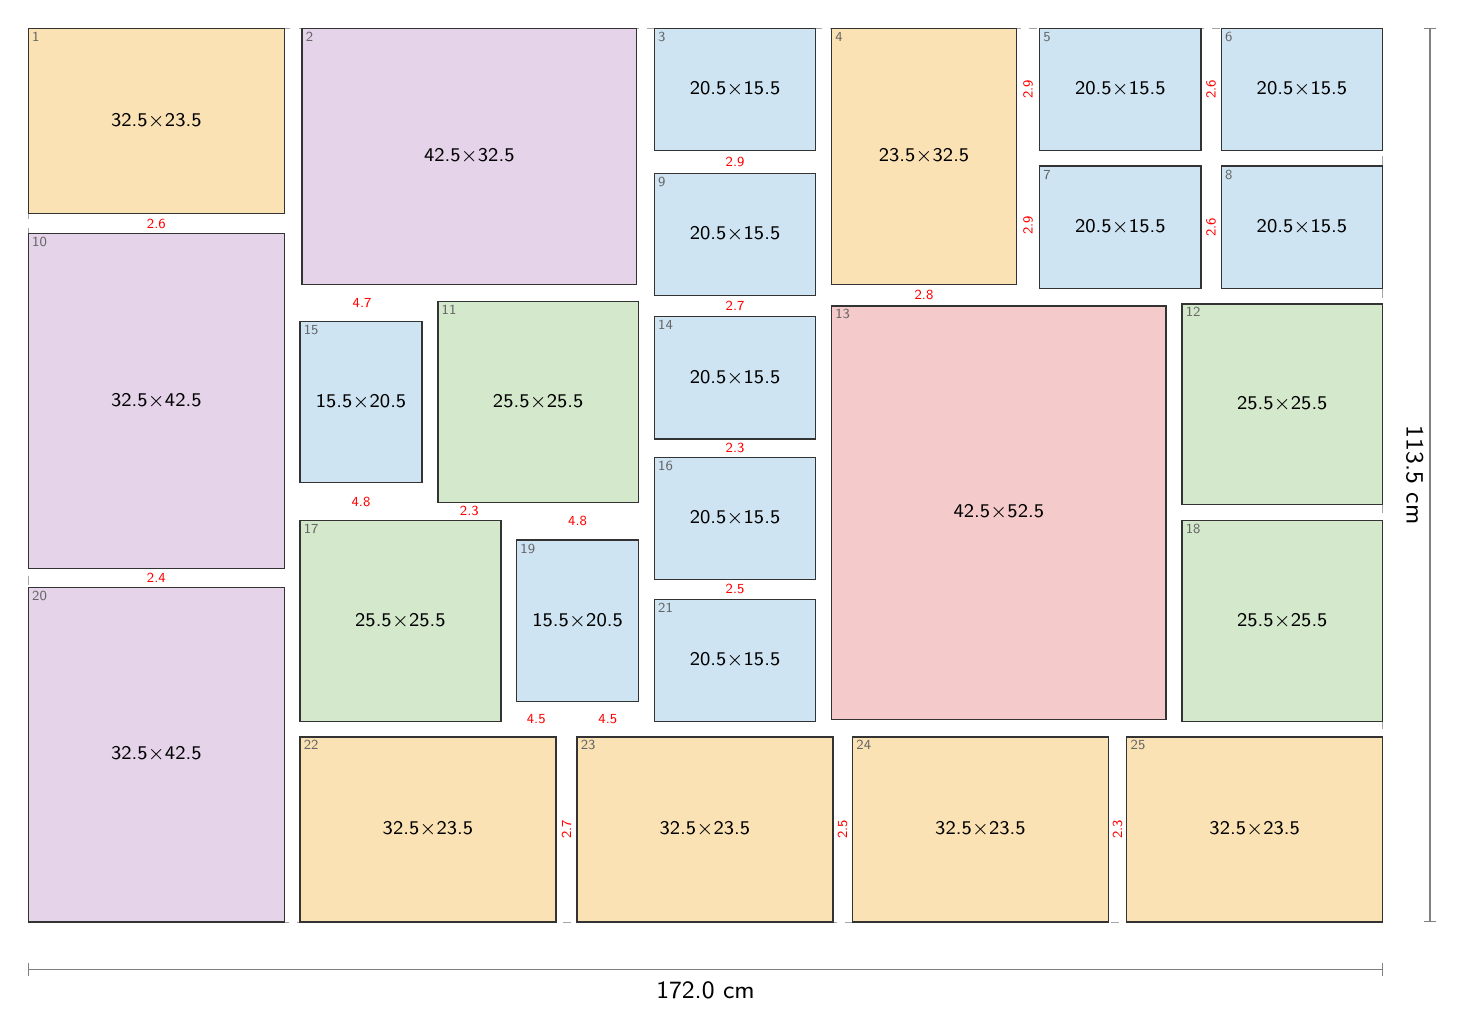
\begin{tikzpicture}[x=1mm, y=-1mm]
\draw[gray!70, dashed, line width=0.4pt] (0,0) rectangle (172.00,113.50);
\filldraw[fill=ft1, draw=black!80, line width=0.5pt] (0.00,0.00) rectangle (32.50,23.50);
\node[align=center, inner sep=0pt] at (16.25,11.75) {\scriptsize 32.5$\times$23.5};
\node[anchor=north west, inner sep=1.2pt, font=\tiny, text=black!60] at (0.00,0.00) {1};
\filldraw[fill=ft3, draw=black!80, line width=0.5pt] (34.75,0.00) rectangle (77.25,32.50);
\node[align=center, inner sep=0pt] at (56.00,16.25) {\scriptsize 42.5$\times$32.5};
\node[anchor=north west, inner sep=1.2pt, font=\tiny, text=black!60] at (34.75,0.00) {2};
\filldraw[fill=ft0, draw=black!80, line width=0.5pt] (79.50,0.00) rectangle (100.00,15.50);
\node[align=center, inner sep=0pt] at (89.75,7.75) {\scriptsize 20.5$\times$15.5};
\node[anchor=north west, inner sep=1.2pt, font=\tiny, text=black!60] at (79.50,0.00) {3};
\filldraw[fill=ft1, draw=black!80, line width=0.5pt] (102.00,0.00) rectangle (125.50,32.50);
\node[align=center, inner sep=0pt] at (113.75,16.25) {\scriptsize 23.5$\times$32.5};
\node[anchor=north west, inner sep=1.2pt, font=\tiny, text=black!60] at (102.00,0.00) {4};
\filldraw[fill=ft0, draw=black!80, line width=0.5pt] (128.43,0.00) rectangle (148.93,15.50);
\node[align=center, inner sep=0pt] at (138.68,7.75) {\scriptsize 20.5$\times$15.5};
\node[anchor=north west, inner sep=1.2pt, font=\tiny, text=black!60] at (128.43,0.00) {5};
\filldraw[fill=ft0, draw=black!80, line width=0.5pt] (151.50,0.00) rectangle (172.00,15.50);
\node[align=center, inner sep=0pt] at (161.75,7.75) {\scriptsize 20.5$\times$15.5};
\node[anchor=north west, inner sep=1.2pt, font=\tiny, text=black!60] at (151.50,0.00) {6};
\filldraw[fill=ft0, draw=black!80, line width=0.5pt] (128.43,17.50) rectangle (148.93,33.00);
\node[align=center, inner sep=0pt] at (138.68,25.25) {\scriptsize 20.5$\times$15.5};
\node[anchor=north west, inner sep=1.2pt, font=\tiny, text=black!60] at (128.43,17.50) {7};
\filldraw[fill=ft0, draw=black!80, line width=0.5pt] (151.50,17.50) rectangle (172.00,33.00);
\node[align=center, inner sep=0pt] at (161.75,25.25) {\scriptsize 20.5$\times$15.5};
\node[anchor=north west, inner sep=1.2pt, font=\tiny, text=black!60] at (151.50,17.50) {8};
\filldraw[fill=ft0, draw=black!80, line width=0.5pt] (79.50,18.41) rectangle (100.00,33.91);
\node[align=center, inner sep=0pt] at (89.75,26.16) {\scriptsize 20.5$\times$15.5};
\node[anchor=north west, inner sep=1.2pt, font=\tiny, text=black!60] at (79.50,18.41) {9};
\filldraw[fill=ft3, draw=black!80, line width=0.5pt] (0.00,26.07) rectangle (32.50,68.57);
\node[align=center, inner sep=0pt] at (16.25,47.32) {\scriptsize 32.5$\times$42.5};
\node[anchor=north west, inner sep=1.2pt, font=\tiny, text=black!60] at (0.00,26.07) {10};
\filldraw[fill=ft2, draw=black!80, line width=0.5pt] (52.00,34.70) rectangle (77.50,60.20);
\node[align=center, inner sep=0pt] at (64.75,47.45) {\scriptsize 25.5$\times$25.5};
\node[anchor=north west, inner sep=1.2pt, font=\tiny, text=black!60] at (52.00,34.70) {11};
\filldraw[fill=ft2, draw=black!80, line width=0.5pt] (146.50,35.00) rectangle (172.00,60.50);
\node[align=center, inner sep=0pt] at (159.25,47.75) {\scriptsize 25.5$\times$25.5};
\node[anchor=north west, inner sep=1.2pt, font=\tiny, text=black!60] at (146.50,35.00) {12};
\filldraw[fill=ft4, draw=black!80, line width=0.5pt] (102.00,35.25) rectangle (144.50,87.75);
\node[align=center, inner sep=0pt] at (123.25,61.50) {\scriptsize 42.5$\times$52.5};
\node[anchor=north west, inner sep=1.2pt, font=\tiny, text=black!60] at (102.00,35.25) {13};
\filldraw[fill=ft0, draw=black!80, line width=0.5pt] (79.50,36.63) rectangle (100.00,52.13);
\node[align=center, inner sep=0pt] at (89.75,44.38) {\scriptsize 20.5$\times$15.5};
\node[anchor=north west, inner sep=1.2pt, font=\tiny, text=black!60] at (79.50,36.63) {14};
\filldraw[fill=ft0, draw=black!80, line width=0.5pt] (34.50,37.20) rectangle (50.00,57.70);
\node[align=center, inner sep=0pt] at (42.25,47.45) {\scriptsize 15.5$\times$20.5};
\node[anchor=north west, inner sep=1.2pt, font=\tiny, text=black!60] at (34.50,37.20) {15};
\filldraw[fill=ft0, draw=black!80, line width=0.5pt] (79.50,54.47) rectangle (100.00,69.97);
\node[align=center, inner sep=0pt] at (89.75,62.22) {\scriptsize 20.5$\times$15.5};
\node[anchor=north west, inner sep=1.2pt, font=\tiny, text=black!60] at (79.50,54.47) {16};
\filldraw[fill=ft2, draw=black!80, line width=0.5pt] (34.50,62.50) rectangle (60.00,88.00);
\node[align=center, inner sep=0pt] at (47.25,75.25) {\scriptsize 25.5$\times$25.5};
\node[anchor=north west, inner sep=1.2pt, font=\tiny, text=black!60] at (34.50,62.50) {17};
\filldraw[fill=ft2, draw=black!80, line width=0.5pt] (146.50,62.50) rectangle (172.00,88.00);
\node[align=center, inner sep=0pt] at (159.25,75.25) {\scriptsize 25.5$\times$25.5};
\node[anchor=north west, inner sep=1.2pt, font=\tiny, text=black!60] at (146.50,62.50) {18};
\filldraw[fill=ft0, draw=black!80, line width=0.5pt] (62.00,65.00) rectangle (77.50,85.50);
\node[align=center, inner sep=0pt] at (69.75,75.25) {\scriptsize 15.5$\times$20.5};
\node[anchor=north west, inner sep=1.2pt, font=\tiny, text=black!60] at (62.00,65.00) {19};
\filldraw[fill=ft3, draw=black!80, line width=0.5pt] (0.00,71.00) rectangle (32.50,113.50);
\node[align=center, inner sep=0pt] at (16.25,92.25) {\scriptsize 32.5$\times$42.5};
\node[anchor=north west, inner sep=1.2pt, font=\tiny, text=black!60] at (0.00,71.00) {20};
\filldraw[fill=ft0, draw=black!80, line width=0.5pt] (79.50,72.50) rectangle (100.00,88.00);
\node[align=center, inner sep=0pt] at (89.75,80.25) {\scriptsize 20.5$\times$15.5};
\node[anchor=north west, inner sep=1.2pt, font=\tiny, text=black!60] at (79.50,72.50) {21};
\filldraw[fill=ft1, draw=black!80, line width=0.5pt] (34.50,90.00) rectangle (67.00,113.50);
\node[align=center, inner sep=0pt] at (50.75,101.75) {\scriptsize 32.5$\times$23.5};
\node[anchor=north west, inner sep=1.2pt, font=\tiny, text=black!60] at (34.50,90.00) {22};
\filldraw[fill=ft1, draw=black!80, line width=0.5pt] (69.67,90.00) rectangle (102.17,113.50);
\node[align=center, inner sep=0pt] at (85.92,101.75) {\scriptsize 32.5$\times$23.5};
\node[anchor=north west, inner sep=1.2pt, font=\tiny, text=black!60] at (69.67,90.00) {23};
\filldraw[fill=ft1, draw=black!80, line width=0.5pt] (104.67,90.00) rectangle (137.17,113.50);
\node[align=center, inner sep=0pt] at (120.92,101.75) {\scriptsize 32.5$\times$23.5};
\node[anchor=north west, inner sep=1.2pt, font=\tiny, text=black!60] at (104.67,90.00) {24};
\filldraw[fill=ft1, draw=black!80, line width=0.5pt] (139.50,90.00) rectangle (172.00,113.50);
\node[align=center, inner sep=0pt] at (155.75,101.75) {\scriptsize 32.5$\times$23.5};
\node[anchor=north west, inner sep=1.2pt, font=\tiny, text=black!60] at (139.50,90.00) {25};
\node[font=\tiny, text=red, fill=white, inner sep=0.3pt] at (16.25,24.78) {2.6};
\node[font=\tiny, text=red, fill=white, inner sep=0.3pt] at (42.38,34.85) {4.7};
\node[font=\tiny, text=red, fill=white, inner sep=0.3pt] at (89.75,16.96) {2.9};
\node[font=\tiny, text=red, fill=white, inner sep=0.3pt, rotate=90] at (126.96,7.75) {2.9};
\node[font=\tiny, text=red, fill=white, inner sep=0.3pt, rotate=90] at (126.96,25.00) {2.9};
\node[font=\tiny, text=red, fill=white, inner sep=0.3pt] at (113.75,33.88) {2.8};
\node[font=\tiny, text=red, fill=white, inner sep=0.3pt, rotate=90] at (150.21,7.75) {2.6};
\node[font=\tiny, text=red, fill=white, inner sep=0.3pt, rotate=90] at (150.21,25.25) {2.6};
\node[font=\tiny, text=red, fill=white, inner sep=0.3pt] at (89.75,35.27) {2.7};
\node[font=\tiny, text=red, fill=white, inner sep=0.3pt] at (16.25,69.78) {2.4};
\node[font=\tiny, text=red, fill=white, inner sep=0.3pt] at (56.00,61.35) {2.3};
\node[font=\tiny, text=red, fill=white, inner sep=0.3pt] at (69.75,62.60) {4.8};
\node[font=\tiny, text=red, fill=white, inner sep=0.3pt] at (89.75,53.30) {2.3};
\node[font=\tiny, text=red, fill=white, inner sep=0.3pt] at (42.25,60.10) {4.8};
\node[font=\tiny, text=red, fill=white, inner sep=0.3pt] at (89.75,71.24) {2.5};
\node[font=\tiny, text=red, fill=white, inner sep=0.3pt] at (64.50,87.75) {4.5};
\node[font=\tiny, text=red, fill=white, inner sep=0.3pt] at (73.59,87.75) {4.5};
\node[font=\tiny, text=red, fill=white, inner sep=0.3pt, rotate=90] at (68.34,101.75) {2.7};
\node[font=\tiny, text=red, fill=white, inner sep=0.3pt, rotate=90] at (103.42,101.75) {2.5};
\node[font=\tiny, text=red, fill=white, inner sep=0.3pt, rotate=90] at (138.34,101.75) {2.3};
\draw[Bar-Bar, gray] (0,119.50) -- (172.00,119.50) node[midway, below=1pt, font=\small, text=black] {172.0 cm};
\draw[Bar-Bar, gray] (178.00,0) -- (178.00,113.50) node[midway, right=1pt, font=\small, text=black, rotate=-90, anchor=north] {113.5 cm};
\end{tikzpicture}\\[4pt]
{\scriptsize Scale 1:10 (1 mm = 1 cm). Red numbers mark gaps that deviate from the nominal gap by more than 0.25 cm. Small grey numbers index the coordinate table.}
\end{minipage}\hfill
\begin{minipage}[t]{0.25\textwidth}\vspace{0pt}
\small
\begin{tabular}{@{}l l@{}}
\toprule
Outer size & 172.0 $\times$ 113.5 cm \\
Nominal gap & 2 cm \\
Actual gaps & 2.0 -- 4.8 cm \\
Max.\ deviation & 2.8 cm \\
Mean deviation & 0.48 cm \\
Border notches & none \\
Corners filled & 4 / 4 \\
Frames used & 25 of 28 \\
Large frames & {\scriptsize 1} \\
Entropy & 0.77 \\
\quad {\scriptsize mix / variety} & {\scriptsize 0.81 / 0.70} \\
\quad {\scriptsize stagger / lines} & {\scriptsize 0.56 / 1.00 (1 through)} \\
\bottomrule
\end{tabular}

\vspace{8pt}
\scriptsize
\begin{tabular}{@{}c l l r r@{}}
\toprule
 & outer w $\times$ h (cm) &  & used & have \\
\midrule
\tikz[baseline=-0.6ex]\fill[ft0,draw=black!60] (0,0) rectangle (1.2ex,1.2ex); & 20.5$\times$15.5 & L & 9 & 9 \\
\tikz[baseline=-0.6ex]\fill[ft0,draw=black!60] (0,0) rectangle (1.2ex,1.2ex); & 15.5$\times$20.5 & P & 2 & 2 \\
\tikz[baseline=-0.6ex]\fill[ft3,draw=black!60] (0,0) rectangle (1.2ex,1.2ex); & 32.5$\times$42.5 & P & 2 & 2 \\
\tikz[baseline=-0.6ex]\fill[ft3,draw=black!60] (0,0) rectangle (1.2ex,1.2ex); & 42.5$\times$32.5 & L & 1 & 1 \\
\tikz[baseline=-0.6ex]\fill[ft1,draw=black!60] (0,0) rectangle (1.2ex,1.2ex); & 32.5$\times$23.5 & L & 5 & 5 \\
\tikz[baseline=-0.6ex]\fill[ft1,draw=black!60] (0,0) rectangle (1.2ex,1.2ex); & 23.5$\times$32.5 & P & 1 & 1 \\
\tikz[baseline=-0.6ex]\fill[ft2,draw=black!60] (0,0) rectangle (1.2ex,1.2ex); & 25.5$\times$25.5 &  & 4 & 5 \\
\tikz[baseline=-0.6ex]\fill[ft4,draw=black!60] (0,0) rectangle (1.2ex,1.2ex); & 42.5$\times$52.5 & P & 1 & 1 \\
\tikz[baseline=-0.6ex]\fill[ft4,draw=black!60] (0,0) rectangle (1.2ex,1.2ex); & 52.5$\times$42.5 & L & 0 & 2 \\
\bottomrule
\end{tabular}

\vspace{8pt}
{\bfseries Positions} (top-left corner, cm)\\[2pt]
\tiny
\begin{tabular}{@{}r l r r@{}}
\toprule
\# & frame w $\times$ h & x & y \\
\midrule
1 & 32.5 $\times$ 23.5 & 0.0 & 0.0 \\
2 & 42.5 $\times$ 32.5 & 34.8 & 0.0 \\
3 & 20.5 $\times$ 15.5 & 79.5 & 0.0 \\
4 & 23.5 $\times$ 32.5 & 102.0 & 0.0 \\
5 & 20.5 $\times$ 15.5 & 128.4 & 0.0 \\
6 & 20.5 $\times$ 15.5 & 151.5 & 0.0 \\
7 & 20.5 $\times$ 15.5 & 128.4 & 17.5 \\
8 & 20.5 $\times$ 15.5 & 151.5 & 17.5 \\
9 & 20.5 $\times$ 15.5 & 79.5 & 18.4 \\
10 & 32.5 $\times$ 42.5 & 0.0 & 26.1 \\
11 & 25.5 $\times$ 25.5 & 52.0 & 34.7 \\
12 & 25.5 $\times$ 25.5 & 146.5 & 35.0 \\
13 & 42.5 $\times$ 52.5 & 102.0 & 35.2 \\
14 & 20.5 $\times$ 15.5 & 79.5 & 36.6 \\
15 & 15.5 $\times$ 20.5 & 34.5 & 37.2 \\
16 & 20.5 $\times$ 15.5 & 79.5 & 54.5 \\
17 & 25.5 $\times$ 25.5 & 34.5 & 62.5 \\
18 & 25.5 $\times$ 25.5 & 146.5 & 62.5 \\
19 & 15.5 $\times$ 20.5 & 62.0 & 65.0 \\
20 & 32.5 $\times$ 42.5 & 0.0 & 71.0 \\
21 & 20.5 $\times$ 15.5 & 79.5 & 72.5 \\
22 & 32.5 $\times$ 23.5 & 34.5 & 90.0 \\
23 & 32.5 $\times$ 23.5 & 69.7 & 90.0 \\
24 & 32.5 $\times$ 23.5 & 104.7 & 90.0 \\
25 & 32.5 $\times$ 23.5 & 139.5 & 90.0 \\
\bottomrule
\end{tabular}
\end{minipage}
\clearpage

\phantomsection\addcontentsline{toc}{subsection}{Layout 5: 177.0 \texorpdfstring{$\times$}{x} 123.0 cm, 25 frames, gap 2 cm, max.\ deviation 3.0 cm}
\label{lay:proportional:5}
\begin{minipage}[t]{0.74\textwidth}\vspace{0pt}
{\LARGE\bfseries Layout 5}\hspace{1.5em}{\large 177.0 $\times$ 123.0 cm \quad gap 2 cm \quad 25 frames}\\[8pt]
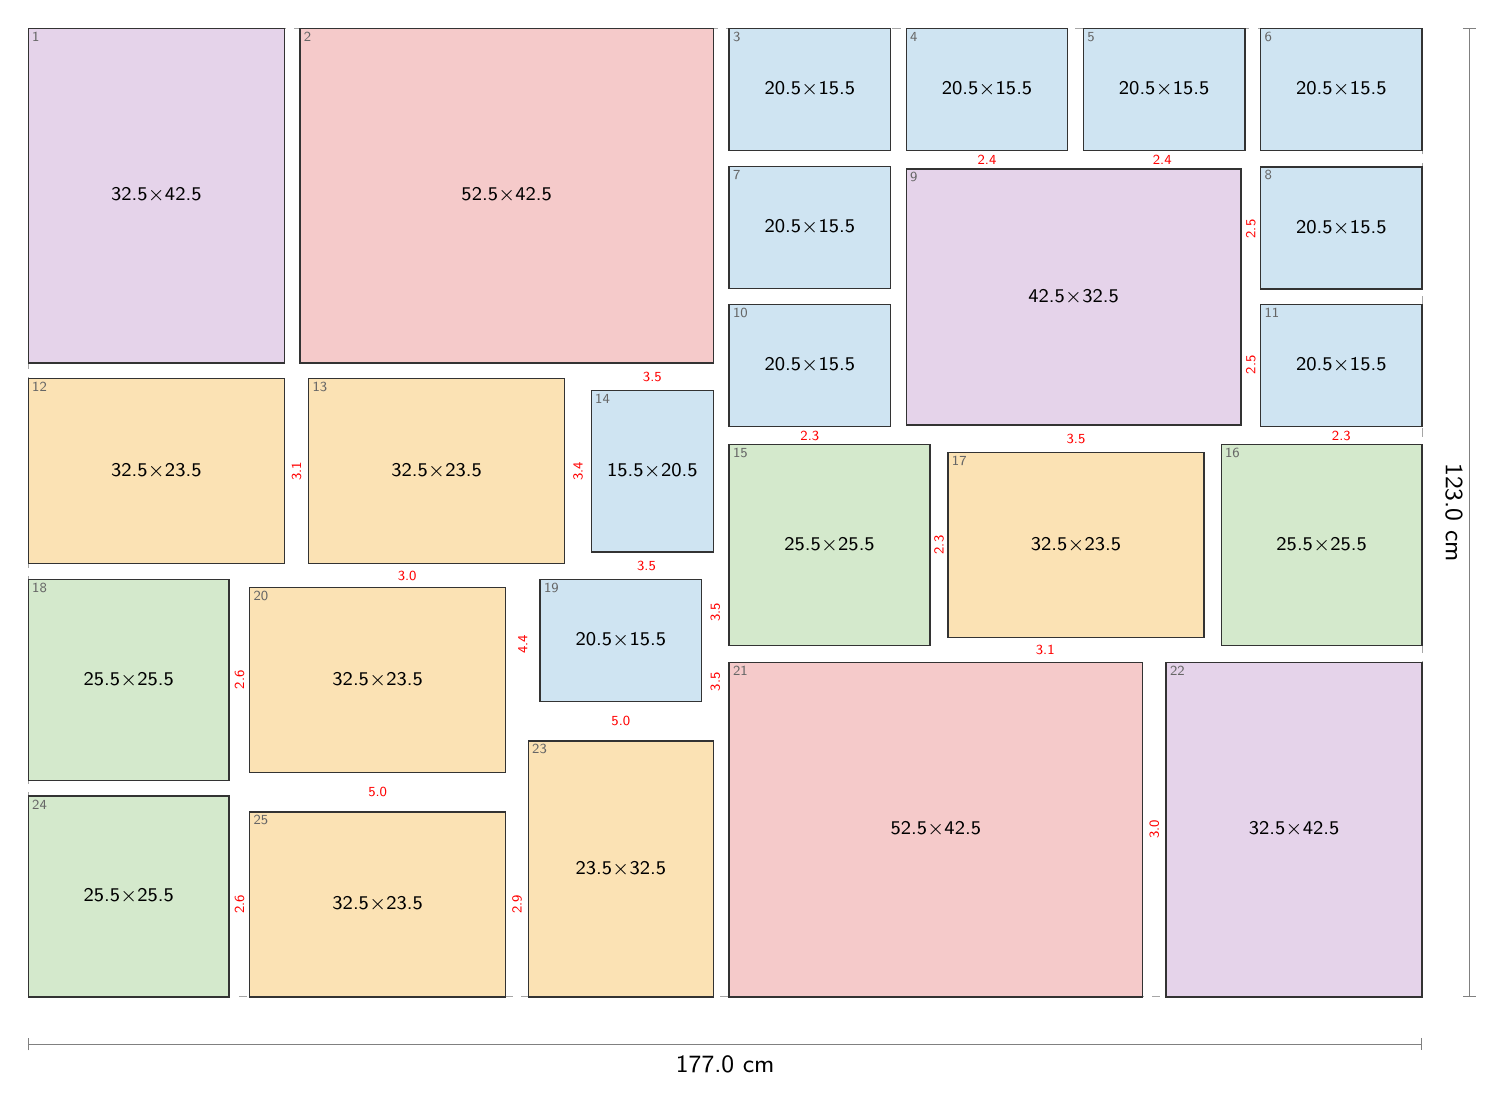
\begin{tikzpicture}[x=1mm, y=-1mm]
\draw[gray!70, dashed, line width=0.4pt] (0,0) rectangle (177.00,123.00);
\filldraw[fill=ft3, draw=black!80, line width=0.5pt] (0.00,0.00) rectangle (32.50,42.50);
\node[align=center, inner sep=0pt] at (16.25,21.25) {\scriptsize 32.5$\times$42.5};
\node[anchor=north west, inner sep=1.2pt, font=\tiny, text=black!60] at (0.00,0.00) {1};
\filldraw[fill=ft4, draw=black!80, line width=0.5pt] (34.50,0.00) rectangle (87.00,42.50);
\node[align=center, inner sep=0pt] at (60.75,21.25) {\scriptsize 52.5$\times$42.5};
\node[anchor=north west, inner sep=1.2pt, font=\tiny, text=black!60] at (34.50,0.00) {2};
\filldraw[fill=ft0, draw=black!80, line width=0.5pt] (89.00,0.00) rectangle (109.50,15.50);
\node[align=center, inner sep=0pt] at (99.25,7.75) {\scriptsize 20.5$\times$15.5};
\node[anchor=north west, inner sep=1.2pt, font=\tiny, text=black!60] at (89.00,0.00) {3};
\filldraw[fill=ft0, draw=black!80, line width=0.5pt] (111.50,0.00) rectangle (132.00,15.50);
\node[align=center, inner sep=0pt] at (121.75,7.75) {\scriptsize 20.5$\times$15.5};
\node[anchor=north west, inner sep=1.2pt, font=\tiny, text=black!60] at (111.50,0.00) {4};
\filldraw[fill=ft0, draw=black!80, line width=0.5pt] (134.00,0.00) rectangle (154.50,15.50);
\node[align=center, inner sep=0pt] at (144.25,7.75) {\scriptsize 20.5$\times$15.5};
\node[anchor=north west, inner sep=1.2pt, font=\tiny, text=black!60] at (134.00,0.00) {5};
\filldraw[fill=ft0, draw=black!80, line width=0.5pt] (156.50,0.00) rectangle (177.00,15.50);
\node[align=center, inner sep=0pt] at (166.75,7.75) {\scriptsize 20.5$\times$15.5};
\node[anchor=north west, inner sep=1.2pt, font=\tiny, text=black!60] at (156.50,0.00) {6};
\filldraw[fill=ft0, draw=black!80, line width=0.5pt] (89.00,17.54) rectangle (109.50,33.04);
\node[align=center, inner sep=0pt] at (99.25,25.29) {\scriptsize 20.5$\times$15.5};
\node[anchor=north west, inner sep=1.2pt, font=\tiny, text=black!60] at (89.00,17.54) {7};
\filldraw[fill=ft0, draw=black!80, line width=0.5pt] (156.50,17.60) rectangle (177.00,33.10);
\node[align=center, inner sep=0pt] at (166.75,25.35) {\scriptsize 20.5$\times$15.5};
\node[anchor=north west, inner sep=1.2pt, font=\tiny, text=black!60] at (156.50,17.60) {8};
\filldraw[fill=ft3, draw=black!80, line width=0.5pt] (111.50,17.85) rectangle (154.00,50.35);
\node[align=center, inner sep=0pt] at (132.75,34.10) {\scriptsize 42.5$\times$32.5};
\node[anchor=north west, inner sep=1.2pt, font=\tiny, text=black!60] at (111.50,17.85) {9};
\filldraw[fill=ft0, draw=black!80, line width=0.5pt] (89.00,35.10) rectangle (109.50,50.60);
\node[align=center, inner sep=0pt] at (99.25,42.85) {\scriptsize 20.5$\times$15.5};
\node[anchor=north west, inner sep=1.2pt, font=\tiny, text=black!60] at (89.00,35.10) {10};
\filldraw[fill=ft0, draw=black!80, line width=0.5pt] (156.50,35.10) rectangle (177.00,50.60);
\node[align=center, inner sep=0pt] at (166.75,42.85) {\scriptsize 20.5$\times$15.5};
\node[anchor=north west, inner sep=1.2pt, font=\tiny, text=black!60] at (156.50,35.10) {11};
\filldraw[fill=ft1, draw=black!80, line width=0.5pt] (0.00,44.50) rectangle (32.50,68.00);
\node[align=center, inner sep=0pt] at (16.25,56.25) {\scriptsize 32.5$\times$23.5};
\node[anchor=north west, inner sep=1.2pt, font=\tiny, text=black!60] at (0.00,44.50) {12};
\filldraw[fill=ft1, draw=black!80, line width=0.5pt] (35.60,44.50) rectangle (68.10,68.00);
\node[align=center, inner sep=0pt] at (51.85,56.25) {\scriptsize 32.5$\times$23.5};
\node[anchor=north west, inner sep=1.2pt, font=\tiny, text=black!60] at (35.60,44.50) {13};
\filldraw[fill=ft0, draw=black!80, line width=0.5pt] (71.50,46.00) rectangle (87.00,66.50);
\node[align=center, inner sep=0pt] at (79.25,56.25) {\scriptsize 15.5$\times$20.5};
\node[anchor=north west, inner sep=1.2pt, font=\tiny, text=black!60] at (71.50,46.00) {14};
\filldraw[fill=ft2, draw=black!80, line width=0.5pt] (89.00,52.86) rectangle (114.50,78.36);
\node[align=center, inner sep=0pt] at (101.75,65.61) {\scriptsize 25.5$\times$25.5};
\node[anchor=north west, inner sep=1.2pt, font=\tiny, text=black!60] at (89.00,52.86) {15};
\filldraw[fill=ft2, draw=black!80, line width=0.5pt] (151.50,52.86) rectangle (177.00,78.36);
\node[align=center, inner sep=0pt] at (164.25,65.61) {\scriptsize 25.5$\times$25.5};
\node[anchor=north west, inner sep=1.2pt, font=\tiny, text=black!60] at (151.50,52.86) {16};
\filldraw[fill=ft1, draw=black!80, line width=0.5pt] (116.80,53.86) rectangle (149.30,77.36);
\node[align=center, inner sep=0pt] at (133.05,65.61) {\scriptsize 32.5$\times$23.5};
\node[anchor=north west, inner sep=1.2pt, font=\tiny, text=black!60] at (116.80,53.86) {17};
\filldraw[fill=ft2, draw=black!80, line width=0.5pt] (0.00,70.00) rectangle (25.50,95.50);
\node[align=center, inner sep=0pt] at (12.75,82.75) {\scriptsize 25.5$\times$25.5};
\node[anchor=north west, inner sep=1.2pt, font=\tiny, text=black!60] at (0.00,70.00) {18};
\filldraw[fill=ft0, draw=black!80, line width=0.5pt] (65.00,70.00) rectangle (85.50,85.50);
\node[align=center, inner sep=0pt] at (75.25,77.75) {\scriptsize 20.5$\times$15.5};
\node[anchor=north west, inner sep=1.2pt, font=\tiny, text=black!60] at (65.00,70.00) {19};
\filldraw[fill=ft1, draw=black!80, line width=0.5pt] (28.11,71.00) rectangle (60.61,94.50);
\node[align=center, inner sep=0pt] at (44.36,82.75) {\scriptsize 32.5$\times$23.5};
\node[anchor=north west, inner sep=1.2pt, font=\tiny, text=black!60] at (28.11,71.00) {20};
\filldraw[fill=ft4, draw=black!80, line width=0.5pt] (89.00,80.50) rectangle (141.50,123.00);
\node[align=center, inner sep=0pt] at (115.25,101.75) {\scriptsize 52.5$\times$42.5};
\node[anchor=north west, inner sep=1.2pt, font=\tiny, text=black!60] at (89.00,80.50) {21};
\filldraw[fill=ft3, draw=black!80, line width=0.5pt] (144.50,80.50) rectangle (177.00,123.00);
\node[align=center, inner sep=0pt] at (160.75,101.75) {\scriptsize 32.5$\times$42.5};
\node[anchor=north west, inner sep=1.2pt, font=\tiny, text=black!60] at (144.50,80.50) {22};
\filldraw[fill=ft1, draw=black!80, line width=0.5pt] (63.50,90.50) rectangle (87.00,123.00);
\node[align=center, inner sep=0pt] at (75.25,106.75) {\scriptsize 23.5$\times$32.5};
\node[anchor=north west, inner sep=1.2pt, font=\tiny, text=black!60] at (63.50,90.50) {23};
\filldraw[fill=ft2, draw=black!80, line width=0.5pt] (0.00,97.50) rectangle (25.50,123.00);
\node[align=center, inner sep=0pt] at (12.75,110.25) {\scriptsize 25.5$\times$25.5};
\node[anchor=north west, inner sep=1.2pt, font=\tiny, text=black!60] at (0.00,97.50) {24};
\filldraw[fill=ft1, draw=black!80, line width=0.5pt] (28.11,99.50) rectangle (60.61,123.00);
\node[align=center, inner sep=0pt] at (44.36,111.25) {\scriptsize 32.5$\times$23.5};
\node[anchor=north west, inner sep=1.2pt, font=\tiny, text=black!60] at (28.11,99.50) {25};
\node[font=\tiny, text=red, fill=white, inner sep=0.3pt] at (79.25,44.25) {3.5};
\node[font=\tiny, text=red, fill=white, inner sep=0.3pt] at (121.75,16.68) {2.4};
\node[font=\tiny, text=red, fill=white, inner sep=0.3pt] at (144.00,16.68) {2.4};
\node[font=\tiny, text=red, fill=white, inner sep=0.3pt, rotate=90] at (155.25,25.48) {2.5};
\node[font=\tiny, text=red, fill=white, inner sep=0.3pt, rotate=90] at (155.25,42.73) {2.5};
\node[font=\tiny, text=red, fill=white, inner sep=0.3pt] at (133.05,52.10) {3.5};
\node[font=\tiny, text=red, fill=white, inner sep=0.3pt] at (99.25,51.73) {2.3};
\node[font=\tiny, text=red, fill=white, inner sep=0.3pt] at (166.75,51.73) {2.3};
\node[font=\tiny, text=red, fill=white, inner sep=0.3pt, rotate=90] at (34.05,56.25) {3.1};
\node[font=\tiny, text=red, fill=white, inner sep=0.3pt, rotate=90] at (69.80,56.25) {3.4};
\node[font=\tiny, text=red, fill=white, inner sep=0.3pt] at (48.11,69.50) {3.0};
\node[font=\tiny, text=red, fill=white, inner sep=0.3pt] at (78.50,68.25) {3.5};
\node[font=\tiny, text=red, fill=white, inner sep=0.3pt, rotate=90] at (115.65,65.61) {2.3};
\node[font=\tiny, text=red, fill=white, inner sep=0.3pt] at (129.15,78.93) {3.1};
\node[font=\tiny, text=red, fill=white, inner sep=0.3pt, rotate=90] at (26.81,82.75) {2.6};
\node[font=\tiny, text=red, fill=white, inner sep=0.3pt, rotate=90] at (87.25,74.18) {3.5};
\node[font=\tiny, text=red, fill=white, inner sep=0.3pt, rotate=90] at (87.25,83.00) {3.5};
\node[font=\tiny, text=red, fill=white, inner sep=0.3pt] at (75.25,88.00) {5.0};
\node[font=\tiny, text=red, fill=white, inner sep=0.3pt, rotate=90] at (62.81,78.25) {4.4};
\node[font=\tiny, text=red, fill=white, inner sep=0.3pt] at (44.36,97.00) {5.0};
\node[font=\tiny, text=red, fill=white, inner sep=0.3pt, rotate=90] at (143.00,101.75) {3.0};
\node[font=\tiny, text=red, fill=white, inner sep=0.3pt, rotate=90] at (26.81,111.25) {2.6};
\node[font=\tiny, text=red, fill=white, inner sep=0.3pt, rotate=90] at (62.06,111.25) {2.9};
\draw[Bar-Bar, gray] (0,129.00) -- (177.00,129.00) node[midway, below=1pt, font=\small, text=black] {177.0 cm};
\draw[Bar-Bar, gray] (183.00,0) -- (183.00,123.00) node[midway, right=1pt, font=\small, text=black, rotate=-90, anchor=north] {123.0 cm};
\end{tikzpicture}\\[4pt]
{\scriptsize Scale 1:10 (1 mm = 1 cm). Red numbers mark gaps that deviate from the nominal gap by more than 0.25 cm. Small grey numbers index the coordinate table.}
\end{minipage}\hfill
\begin{minipage}[t]{0.25\textwidth}\vspace{0pt}
\small
\begin{tabular}{@{}l l@{}}
\toprule
Outer size & 177.0 $\times$ 123.0 cm \\
Nominal gap & 2 cm \\
Actual gaps & 2.0 -- 5.0 cm \\
Max.\ deviation & 3.0 cm \\
Mean deviation & 0.60 cm \\
Border notches & none \\
Corners filled & 4 / 4 \\
Frames used & 25 of 28 \\
Large frames & {\scriptsize 2, not touching, min.\ dist.\ 97 cm} \\
Entropy & 0.78 \\
\quad {\scriptsize mix / variety} & {\scriptsize 0.81 / 0.74} \\
\quad {\scriptsize stagger / lines} & {\scriptsize 0.57 / 1.00 (1 through)} \\
\bottomrule
\end{tabular}

\vspace{8pt}
\scriptsize
\begin{tabular}{@{}c l l r r@{}}
\toprule
 & outer w $\times$ h (cm) &  & used & have \\
\midrule
\tikz[baseline=-0.6ex]\fill[ft0,draw=black!60] (0,0) rectangle (1.2ex,1.2ex); & 20.5$\times$15.5 & L & 9 & 9 \\
\tikz[baseline=-0.6ex]\fill[ft0,draw=black!60] (0,0) rectangle (1.2ex,1.2ex); & 15.5$\times$20.5 & P & 1 & 2 \\
\tikz[baseline=-0.6ex]\fill[ft3,draw=black!60] (0,0) rectangle (1.2ex,1.2ex); & 32.5$\times$42.5 & P & 2 & 2 \\
\tikz[baseline=-0.6ex]\fill[ft3,draw=black!60] (0,0) rectangle (1.2ex,1.2ex); & 42.5$\times$32.5 & L & 1 & 1 \\
\tikz[baseline=-0.6ex]\fill[ft1,draw=black!60] (0,0) rectangle (1.2ex,1.2ex); & 32.5$\times$23.5 & L & 5 & 5 \\
\tikz[baseline=-0.6ex]\fill[ft1,draw=black!60] (0,0) rectangle (1.2ex,1.2ex); & 23.5$\times$32.5 & P & 1 & 1 \\
\tikz[baseline=-0.6ex]\fill[ft2,draw=black!60] (0,0) rectangle (1.2ex,1.2ex); & 25.5$\times$25.5 &  & 4 & 5 \\
\tikz[baseline=-0.6ex]\fill[ft4,draw=black!60] (0,0) rectangle (1.2ex,1.2ex); & 42.5$\times$52.5 & P & 0 & 1 \\
\tikz[baseline=-0.6ex]\fill[ft4,draw=black!60] (0,0) rectangle (1.2ex,1.2ex); & 52.5$\times$42.5 & L & 2 & 2 \\
\bottomrule
\end{tabular}

\vspace{8pt}
{\bfseries Positions} (top-left corner, cm)\\[2pt]
\tiny
\begin{tabular}{@{}r l r r@{}}
\toprule
\# & frame w $\times$ h & x & y \\
\midrule
1 & 32.5 $\times$ 42.5 & 0.0 & 0.0 \\
2 & 52.5 $\times$ 42.5 & 34.5 & 0.0 \\
3 & 20.5 $\times$ 15.5 & 89.0 & 0.0 \\
4 & 20.5 $\times$ 15.5 & 111.5 & 0.0 \\
5 & 20.5 $\times$ 15.5 & 134.0 & 0.0 \\
6 & 20.5 $\times$ 15.5 & 156.5 & 0.0 \\
7 & 20.5 $\times$ 15.5 & 89.0 & 17.5 \\
8 & 20.5 $\times$ 15.5 & 156.5 & 17.6 \\
9 & 42.5 $\times$ 32.5 & 111.5 & 17.9 \\
10 & 20.5 $\times$ 15.5 & 89.0 & 35.1 \\
11 & 20.5 $\times$ 15.5 & 156.5 & 35.1 \\
12 & 32.5 $\times$ 23.5 & 0.0 & 44.5 \\
13 & 32.5 $\times$ 23.5 & 35.6 & 44.5 \\
14 & 15.5 $\times$ 20.5 & 71.5 & 46.0 \\
15 & 25.5 $\times$ 25.5 & 89.0 & 52.9 \\
16 & 25.5 $\times$ 25.5 & 151.5 & 52.9 \\
17 & 32.5 $\times$ 23.5 & 116.8 & 53.9 \\
18 & 25.5 $\times$ 25.5 & 0.0 & 70.0 \\
19 & 20.5 $\times$ 15.5 & 65.0 & 70.0 \\
20 & 32.5 $\times$ 23.5 & 28.1 & 71.0 \\
21 & 52.5 $\times$ 42.5 & 89.0 & 80.5 \\
22 & 32.5 $\times$ 42.5 & 144.5 & 80.5 \\
23 & 23.5 $\times$ 32.5 & 63.5 & 90.5 \\
24 & 25.5 $\times$ 25.5 & 0.0 & 97.5 \\
25 & 32.5 $\times$ 23.5 & 28.1 & 99.5 \\
\bottomrule
\end{tabular}
\end{minipage}
\clearpage

\phantomsection\addcontentsline{toc}{subsection}{Layout 6: 184.0 \texorpdfstring{$\times$}{x} 115.0 cm, 23 frames, gap 2 cm, max.\ deviation 2.2 cm}
\label{lay:proportional:6}
\begin{minipage}[t]{0.74\textwidth}\vspace{0pt}
{\LARGE\bfseries Layout 6}\hspace{1.5em}{\large 184.0 $\times$ 115.0 cm \quad gap 2 cm \quad 23 frames}\\[8pt]
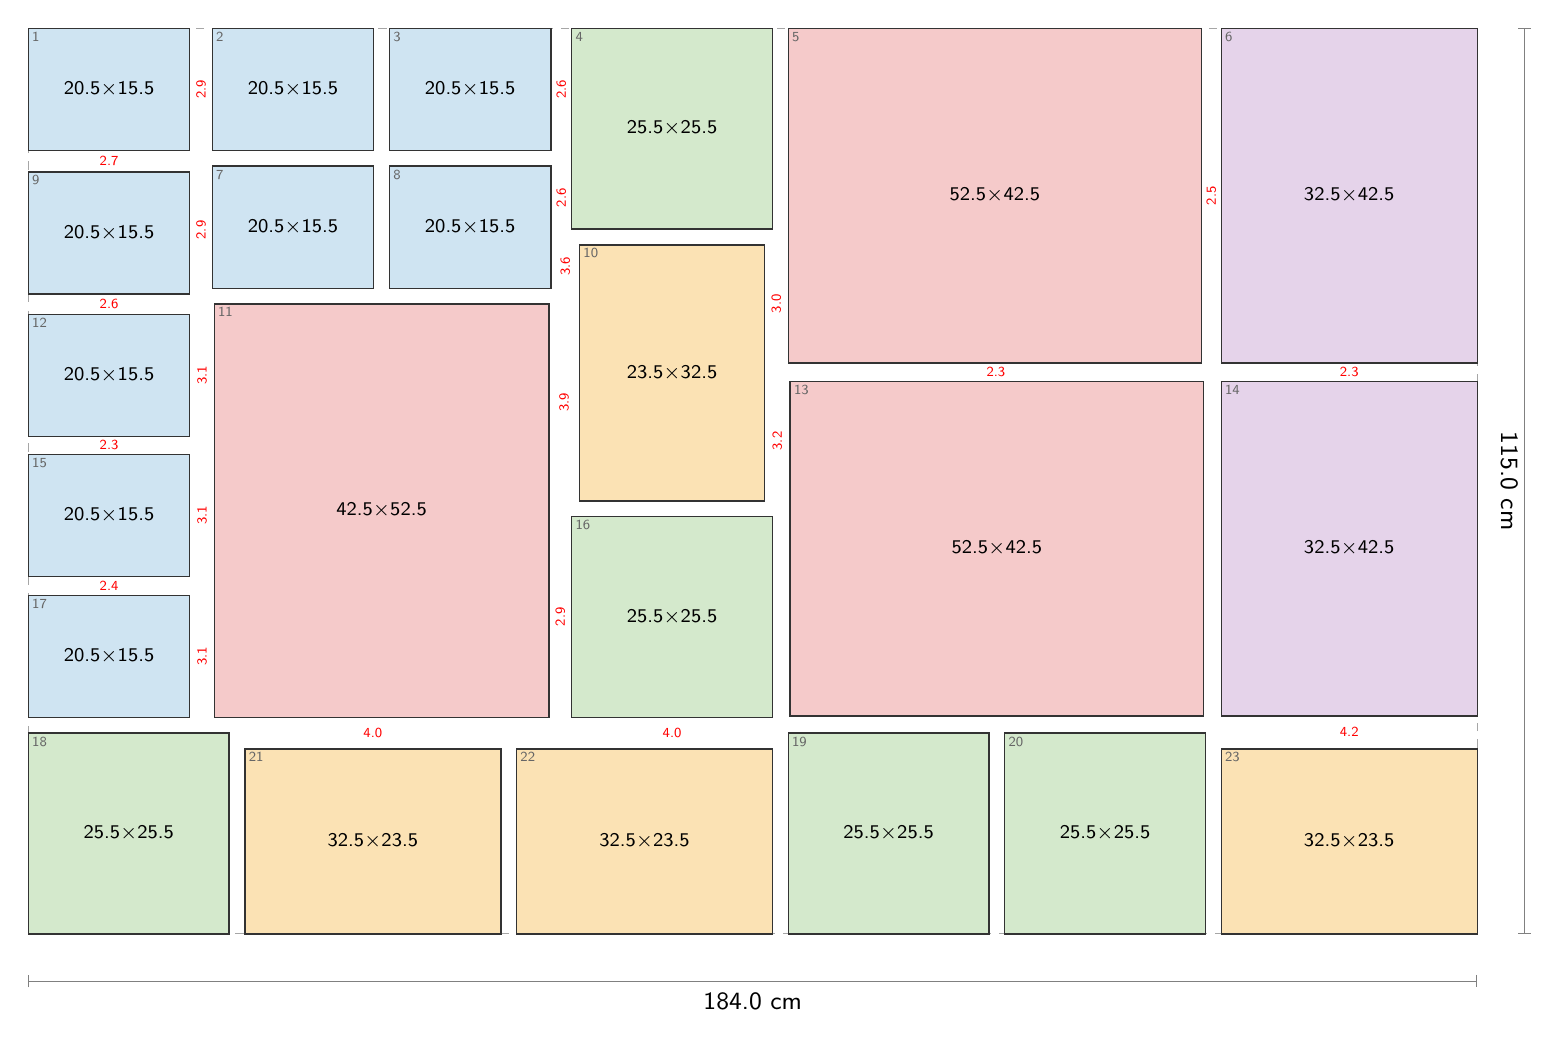
\begin{tikzpicture}[x=1mm, y=-1mm]
\draw[gray!70, dashed, line width=0.4pt] (0,0) rectangle (184.00,115.00);
\filldraw[fill=ft0, draw=black!80, line width=0.5pt] (0.00,0.00) rectangle (20.50,15.50);
\node[align=center, inner sep=0pt] at (10.25,7.75) {\scriptsize 20.5$\times$15.5};
\node[anchor=north west, inner sep=1.2pt, font=\tiny, text=black!60] at (0.00,0.00) {1};
\filldraw[fill=ft0, draw=black!80, line width=0.5pt] (23.36,0.00) rectangle (43.86,15.50);
\node[align=center, inner sep=0pt] at (33.61,7.75) {\scriptsize 20.5$\times$15.5};
\node[anchor=north west, inner sep=1.2pt, font=\tiny, text=black!60] at (23.36,0.00) {2};
\filldraw[fill=ft0, draw=black!80, line width=0.5pt] (45.86,0.00) rectangle (66.36,15.50);
\node[align=center, inner sep=0pt] at (56.11,7.75) {\scriptsize 20.5$\times$15.5};
\node[anchor=north west, inner sep=1.2pt, font=\tiny, text=black!60] at (45.86,0.00) {3};
\filldraw[fill=ft2, draw=black!80, line width=0.5pt] (69.00,0.00) rectangle (94.50,25.50);
\node[align=center, inner sep=0pt] at (81.75,12.75) {\scriptsize 25.5$\times$25.5};
\node[anchor=north west, inner sep=1.2pt, font=\tiny, text=black!60] at (69.00,0.00) {4};
\filldraw[fill=ft4, draw=black!80, line width=0.5pt] (96.50,0.00) rectangle (149.00,42.50);
\node[align=center, inner sep=0pt] at (122.75,21.25) {\scriptsize 52.5$\times$42.5};
\node[anchor=north west, inner sep=1.2pt, font=\tiny, text=black!60] at (96.50,0.00) {5};
\filldraw[fill=ft3, draw=black!80, line width=0.5pt] (151.50,0.00) rectangle (184.00,42.50);
\node[align=center, inner sep=0pt] at (167.75,21.25) {\scriptsize 32.5$\times$42.5};
\node[anchor=north west, inner sep=1.2pt, font=\tiny, text=black!60] at (151.50,0.00) {6};
\filldraw[fill=ft0, draw=black!80, line width=0.5pt] (23.36,17.50) rectangle (43.86,33.00);
\node[align=center, inner sep=0pt] at (33.61,25.25) {\scriptsize 20.5$\times$15.5};
\node[anchor=north west, inner sep=1.2pt, font=\tiny, text=black!60] at (23.36,17.50) {7};
\filldraw[fill=ft0, draw=black!80, line width=0.5pt] (45.86,17.50) rectangle (66.36,33.00);
\node[align=center, inner sep=0pt] at (56.11,25.25) {\scriptsize 20.5$\times$15.5};
\node[anchor=north west, inner sep=1.2pt, font=\tiny, text=black!60] at (45.86,17.50) {8};
\filldraw[fill=ft0, draw=black!80, line width=0.5pt] (0.00,18.23) rectangle (20.50,33.73);
\node[align=center, inner sep=0pt] at (10.25,25.98) {\scriptsize 20.5$\times$15.5};
\node[anchor=north west, inner sep=1.2pt, font=\tiny, text=black!60] at (0.00,18.23) {9};
\filldraw[fill=ft1, draw=black!80, line width=0.5pt] (70.00,27.50) rectangle (93.50,60.00);
\node[align=center, inner sep=0pt] at (81.75,43.75) {\scriptsize 23.5$\times$32.5};
\node[anchor=north west, inner sep=1.2pt, font=\tiny, text=black!60] at (70.00,27.50) {10};
\filldraw[fill=ft4, draw=black!80, line width=0.5pt] (23.61,35.00) rectangle (66.11,87.50);
\node[align=center, inner sep=0pt] at (44.86,61.25) {\scriptsize 42.5$\times$52.5};
\node[anchor=north west, inner sep=1.2pt, font=\tiny, text=black!60] at (23.61,35.00) {11};
\filldraw[fill=ft0, draw=black!80, line width=0.5pt] (0.00,36.31) rectangle (20.50,51.81);
\node[align=center, inner sep=0pt] at (10.25,44.06) {\scriptsize 20.5$\times$15.5};
\node[anchor=north west, inner sep=1.2pt, font=\tiny, text=black!60] at (0.00,36.31) {12};
\filldraw[fill=ft4, draw=black!80, line width=0.5pt] (96.75,44.82) rectangle (149.25,87.32);
\node[align=center, inner sep=0pt] at (123.00,66.07) {\scriptsize 52.5$\times$42.5};
\node[anchor=north west, inner sep=1.2pt, font=\tiny, text=black!60] at (96.75,44.82) {13};
\filldraw[fill=ft3, draw=black!80, line width=0.5pt] (151.50,44.82) rectangle (184.00,87.32);
\node[align=center, inner sep=0pt] at (167.75,66.07) {\scriptsize 32.5$\times$42.5};
\node[anchor=north west, inner sep=1.2pt, font=\tiny, text=black!60] at (151.50,44.82) {14};
\filldraw[fill=ft0, draw=black!80, line width=0.5pt] (0.00,54.08) rectangle (20.50,69.58);
\node[align=center, inner sep=0pt] at (10.25,61.83) {\scriptsize 20.5$\times$15.5};
\node[anchor=north west, inner sep=1.2pt, font=\tiny, text=black!60] at (0.00,54.08) {15};
\filldraw[fill=ft2, draw=black!80, line width=0.5pt] (69.00,62.00) rectangle (94.50,87.50);
\node[align=center, inner sep=0pt] at (81.75,74.75) {\scriptsize 25.5$\times$25.5};
\node[anchor=north west, inner sep=1.2pt, font=\tiny, text=black!60] at (69.00,62.00) {16};
\filldraw[fill=ft0, draw=black!80, line width=0.5pt] (0.00,72.00) rectangle (20.50,87.50);
\node[align=center, inner sep=0pt] at (10.25,79.75) {\scriptsize 20.5$\times$15.5};
\node[anchor=north west, inner sep=1.2pt, font=\tiny, text=black!60] at (0.00,72.00) {17};
\filldraw[fill=ft2, draw=black!80, line width=0.5pt] (0.00,89.50) rectangle (25.50,115.00);
\node[align=center, inner sep=0pt] at (12.75,102.25) {\scriptsize 25.5$\times$25.5};
\node[anchor=north west, inner sep=1.2pt, font=\tiny, text=black!60] at (0.00,89.50) {18};
\filldraw[fill=ft2, draw=black!80, line width=0.5pt] (96.50,89.50) rectangle (122.00,115.00);
\node[align=center, inner sep=0pt] at (109.25,102.25) {\scriptsize 25.5$\times$25.5};
\node[anchor=north west, inner sep=1.2pt, font=\tiny, text=black!60] at (96.50,89.50) {19};
\filldraw[fill=ft2, draw=black!80, line width=0.5pt] (124.00,89.50) rectangle (149.50,115.00);
\node[align=center, inner sep=0pt] at (136.75,102.25) {\scriptsize 25.5$\times$25.5};
\node[anchor=north west, inner sep=1.2pt, font=\tiny, text=black!60] at (124.00,89.50) {20};
\filldraw[fill=ft1, draw=black!80, line width=0.5pt] (27.50,91.50) rectangle (60.00,115.00);
\node[align=center, inner sep=0pt] at (43.75,103.25) {\scriptsize 32.5$\times$23.5};
\node[anchor=north west, inner sep=1.2pt, font=\tiny, text=black!60] at (27.50,91.50) {21};
\filldraw[fill=ft1, draw=black!80, line width=0.5pt] (62.00,91.50) rectangle (94.50,115.00);
\node[align=center, inner sep=0pt] at (78.25,103.25) {\scriptsize 32.5$\times$23.5};
\node[anchor=north west, inner sep=1.2pt, font=\tiny, text=black!60] at (62.00,91.50) {22};
\filldraw[fill=ft1, draw=black!80, line width=0.5pt] (151.50,91.50) rectangle (184.00,115.00);
\node[align=center, inner sep=0pt] at (167.75,103.25) {\scriptsize 32.5$\times$23.5};
\node[anchor=north west, inner sep=1.2pt, font=\tiny, text=black!60] at (151.50,91.50) {23};
\node[font=\tiny, text=red, fill=white, inner sep=0.3pt, rotate=90] at (21.93,7.75) {2.9};
\node[font=\tiny, text=red, fill=white, inner sep=0.3pt] at (10.25,16.86) {2.7};
\node[font=\tiny, text=red, fill=white, inner sep=0.3pt, rotate=90] at (67.68,7.75) {2.6};
\node[font=\tiny, text=red, fill=white, inner sep=0.3pt, rotate=90] at (150.25,21.25) {2.5};
\node[font=\tiny, text=red, fill=white, inner sep=0.3pt] at (122.88,43.66) {2.3};
\node[font=\tiny, text=red, fill=white, inner sep=0.3pt] at (167.75,43.66) {2.3};
\node[font=\tiny, text=red, fill=white, inner sep=0.3pt, rotate=90] at (67.68,21.50) {2.6};
\node[font=\tiny, text=red, fill=white, inner sep=0.3pt, rotate=90] at (68.18,30.25) {3.6};
\node[font=\tiny, text=red, fill=white, inner sep=0.3pt, rotate=90] at (21.93,25.61) {2.9};
\node[font=\tiny, text=red, fill=white, inner sep=0.3pt] at (10.25,35.02) {2.6};
\node[font=\tiny, text=red, fill=white, inner sep=0.3pt, rotate=90] at (95.00,35.00) {3.0};
\node[font=\tiny, text=red, fill=white, inner sep=0.3pt, rotate=90] at (95.12,52.41) {3.2};
\node[font=\tiny, text=red, fill=white, inner sep=0.3pt, rotate=90] at (68.05,47.50) {3.9};
\node[font=\tiny, text=red, fill=white, inner sep=0.3pt, rotate=90] at (67.55,74.75) {2.9};
\node[font=\tiny, text=red, fill=white, inner sep=0.3pt] at (43.75,89.50) {4.0};
\node[font=\tiny, text=red, fill=white, inner sep=0.3pt, rotate=90] at (22.05,44.06) {3.1};
\node[font=\tiny, text=red, fill=white, inner sep=0.3pt] at (10.25,52.94) {2.3};
\node[font=\tiny, text=red, fill=white, inner sep=0.3pt] at (167.75,89.41) {4.2};
\node[font=\tiny, text=red, fill=white, inner sep=0.3pt, rotate=90] at (22.05,61.83) {3.1};
\node[font=\tiny, text=red, fill=white, inner sep=0.3pt] at (10.25,70.79) {2.4};
\node[font=\tiny, text=red, fill=white, inner sep=0.3pt] at (81.75,89.50) {4.0};
\node[font=\tiny, text=red, fill=white, inner sep=0.3pt, rotate=90] at (22.05,79.75) {3.1};
\draw[Bar-Bar, gray] (0,121.00) -- (184.00,121.00) node[midway, below=1pt, font=\small, text=black] {184.0 cm};
\draw[Bar-Bar, gray] (190.00,0) -- (190.00,115.00) node[midway, right=1pt, font=\small, text=black, rotate=-90, anchor=north] {115.0 cm};
\end{tikzpicture}\\[4pt]
{\scriptsize Scale 1:10 (1 mm = 1 cm). Red numbers mark gaps that deviate from the nominal gap by more than 0.25 cm. Small grey numbers index the coordinate table.}
\end{minipage}\hfill
\begin{minipage}[t]{0.25\textwidth}\vspace{0pt}
\small
\begin{tabular}{@{}l l@{}}
\toprule
Outer size & 184.0 $\times$ 115.0 cm \\
Nominal gap & 2 cm \\
Actual gaps & 2.0 -- 4.2 cm \\
Max.\ deviation & 2.2 cm \\
Mean deviation & 0.57 cm \\
Border notches & right 4 cm \\
Corners filled & 4 / 4 \\
Frames used & 23 of 28 \\
Large frames & {\scriptsize 3, touching 1$\times$ (52 cm), min.\ dist.\ 45 cm} \\
Entropy & 0.59 \\
\quad {\scriptsize mix / variety} & {\scriptsize 0.76 / 0.56} \\
\quad {\scriptsize stagger / lines} & {\scriptsize 0.52 / 0.50 (3 through)} \\
\bottomrule
\end{tabular}

\vspace{8pt}
\scriptsize
\begin{tabular}{@{}c l l r r@{}}
\toprule
 & outer w $\times$ h (cm) &  & used & have \\
\midrule
\tikz[baseline=-0.6ex]\fill[ft0,draw=black!60] (0,0) rectangle (1.2ex,1.2ex); & 20.5$\times$15.5 & L & 9 & 9 \\
\tikz[baseline=-0.6ex]\fill[ft0,draw=black!60] (0,0) rectangle (1.2ex,1.2ex); & 15.5$\times$20.5 & P & 0 & 2 \\
\tikz[baseline=-0.6ex]\fill[ft3,draw=black!60] (0,0) rectangle (1.2ex,1.2ex); & 32.5$\times$42.5 & P & 2 & 2 \\
\tikz[baseline=-0.6ex]\fill[ft3,draw=black!60] (0,0) rectangle (1.2ex,1.2ex); & 42.5$\times$32.5 & L & 0 & 1 \\
\tikz[baseline=-0.6ex]\fill[ft1,draw=black!60] (0,0) rectangle (1.2ex,1.2ex); & 32.5$\times$23.5 & L & 3 & 5 \\
\tikz[baseline=-0.6ex]\fill[ft1,draw=black!60] (0,0) rectangle (1.2ex,1.2ex); & 23.5$\times$32.5 & P & 1 & 1 \\
\tikz[baseline=-0.6ex]\fill[ft2,draw=black!60] (0,0) rectangle (1.2ex,1.2ex); & 25.5$\times$25.5 &  & 5 & 5 \\
\tikz[baseline=-0.6ex]\fill[ft4,draw=black!60] (0,0) rectangle (1.2ex,1.2ex); & 42.5$\times$52.5 & P & 1 & 1 \\
\tikz[baseline=-0.6ex]\fill[ft4,draw=black!60] (0,0) rectangle (1.2ex,1.2ex); & 52.5$\times$42.5 & L & 2 & 2 \\
\bottomrule
\end{tabular}

\vspace{8pt}
{\bfseries Positions} (top-left corner, cm)\\[2pt]
\tiny
\begin{tabular}{@{}r l r r@{}}
\toprule
\# & frame w $\times$ h & x & y \\
\midrule
1 & 20.5 $\times$ 15.5 & 0.0 & 0.0 \\
2 & 20.5 $\times$ 15.5 & 23.4 & 0.0 \\
3 & 20.5 $\times$ 15.5 & 45.9 & 0.0 \\
4 & 25.5 $\times$ 25.5 & 69.0 & 0.0 \\
5 & 52.5 $\times$ 42.5 & 96.5 & 0.0 \\
6 & 32.5 $\times$ 42.5 & 151.5 & 0.0 \\
7 & 20.5 $\times$ 15.5 & 23.4 & 17.5 \\
8 & 20.5 $\times$ 15.5 & 45.9 & 17.5 \\
9 & 20.5 $\times$ 15.5 & 0.0 & 18.2 \\
10 & 23.5 $\times$ 32.5 & 70.0 & 27.5 \\
11 & 42.5 $\times$ 52.5 & 23.6 & 35.0 \\
12 & 20.5 $\times$ 15.5 & 0.0 & 36.3 \\
13 & 52.5 $\times$ 42.5 & 96.8 & 44.8 \\
14 & 32.5 $\times$ 42.5 & 151.5 & 44.8 \\
15 & 20.5 $\times$ 15.5 & 0.0 & 54.1 \\
16 & 25.5 $\times$ 25.5 & 69.0 & 62.0 \\
17 & 20.5 $\times$ 15.5 & 0.0 & 72.0 \\
18 & 25.5 $\times$ 25.5 & 0.0 & 89.5 \\
19 & 25.5 $\times$ 25.5 & 96.5 & 89.5 \\
20 & 25.5 $\times$ 25.5 & 124.0 & 89.5 \\
21 & 32.5 $\times$ 23.5 & 27.5 & 91.5 \\
22 & 32.5 $\times$ 23.5 & 62.0 & 91.5 \\
23 & 32.5 $\times$ 23.5 & 151.5 & 91.5 \\
\bottomrule
\end{tabular}
\end{minipage}
\clearpage

\phantomsection\addcontentsline{toc}{subsection}{Layout 7: 170.5 \texorpdfstring{$\times$}{x} 123.5 cm, 23 frames, gap 2 cm, max.\ deviation 3.0 cm}
\label{lay:proportional:7}
\begin{minipage}[t]{0.74\textwidth}\vspace{0pt}
{\LARGE\bfseries Layout 7}\hspace{1.5em}{\large 170.5 $\times$ 123.5 cm \quad gap 2 cm \quad 23 frames}\\[8pt]
\begin{tikzpicture}[x=1mm, y=-1mm]
\draw[gray!70, dashed, line width=0.4pt] (0,0) rectangle (170.50,123.50);
\filldraw[fill=ft1, draw=black!80, line width=0.5pt] (0.00,0.00) rectangle (32.50,23.50);
\node[align=center, inner sep=0pt] at (16.25,11.75) {\scriptsize 32.5$\times$23.5};
\node[anchor=north west, inner sep=1.2pt, font=\tiny, text=black!60] at (0.00,0.00) {1};
\filldraw[fill=ft1, draw=black!80, line width=0.5pt] (34.50,0.00) rectangle (67.00,23.50);
\node[align=center, inner sep=0pt] at (50.75,11.75) {\scriptsize 32.5$\times$23.5};
\node[anchor=north west, inner sep=1.2pt, font=\tiny, text=black!60] at (34.50,0.00) {2};
\filldraw[fill=ft1, draw=black!80, line width=0.5pt] (69.00,0.00) rectangle (101.50,23.50);
\node[align=center, inner sep=0pt] at (85.25,11.75) {\scriptsize 32.5$\times$23.5};
\node[anchor=north west, inner sep=1.2pt, font=\tiny, text=black!60] at (69.00,0.00) {3};
\filldraw[fill=ft1, draw=black!80, line width=0.5pt] (103.50,0.00) rectangle (136.00,23.50);
\node[align=center, inner sep=0pt] at (119.75,11.75) {\scriptsize 32.5$\times$23.5};
\node[anchor=north west, inner sep=1.2pt, font=\tiny, text=black!60] at (103.50,0.00) {4};
\filldraw[fill=ft1, draw=black!80, line width=0.5pt] (138.00,0.00) rectangle (170.50,23.50);
\node[align=center, inner sep=0pt] at (154.25,11.75) {\scriptsize 32.5$\times$23.5};
\node[anchor=north west, inner sep=1.2pt, font=\tiny, text=black!60] at (138.00,0.00) {5};
\filldraw[fill=ft2, draw=black!80, line width=0.5pt] (0.00,25.50) rectangle (25.50,51.00);
\node[align=center, inner sep=0pt] at (12.75,38.25) {\scriptsize 25.5$\times$25.5};
\node[anchor=north west, inner sep=1.2pt, font=\tiny, text=black!60] at (0.00,25.50) {6};
\filldraw[fill=ft2, draw=black!80, line width=0.5pt] (28.19,25.50) rectangle (53.69,51.00);
\node[align=center, inner sep=0pt] at (40.94,38.25) {\scriptsize 25.5$\times$25.5};
\node[anchor=north west, inner sep=1.2pt, font=\tiny, text=black!60] at (28.19,25.50) {7};
\filldraw[fill=ft1, draw=black!80, line width=0.5pt] (56.74,25.50) rectangle (80.24,58.00);
\node[align=center, inner sep=0pt] at (68.49,41.75) {\scriptsize 23.5$\times$32.5};
\node[anchor=north west, inner sep=1.2pt, font=\tiny, text=black!60] at (56.74,25.50) {8};
\filldraw[fill=ft0, draw=black!80, line width=0.5pt] (82.74,25.50) rectangle (103.24,41.00);
\node[align=center, inner sep=0pt] at (92.99,33.25) {\scriptsize 20.5$\times$15.5};
\node[anchor=north west, inner sep=1.2pt, font=\tiny, text=black!60] at (82.74,25.50) {9};
\filldraw[fill=ft0, draw=black!80, line width=0.5pt] (105.33,25.50) rectangle (125.83,41.00);
\node[align=center, inner sep=0pt] at (115.58,33.25) {\scriptsize 20.5$\times$15.5};
\node[anchor=north west, inner sep=1.2pt, font=\tiny, text=black!60] at (105.33,25.50) {10};
\filldraw[fill=ft4, draw=black!80, line width=0.5pt] (128.00,25.50) rectangle (170.50,78.00);
\node[align=center, inner sep=0pt] at (149.25,51.75) {\scriptsize 42.5$\times$52.5};
\node[anchor=north west, inner sep=1.2pt, font=\tiny, text=black!60] at (128.00,25.50) {11};
\filldraw[fill=ft0, draw=black!80, line width=0.5pt] (82.74,43.78) rectangle (103.24,59.28);
\node[align=center, inner sep=0pt] at (92.99,51.53) {\scriptsize 20.5$\times$15.5};
\node[anchor=north west, inner sep=1.2pt, font=\tiny, text=black!60] at (82.74,43.78) {12};
\filldraw[fill=ft0, draw=black!80, line width=0.5pt] (105.33,43.78) rectangle (125.83,59.28);
\node[align=center, inner sep=0pt] at (115.58,51.53) {\scriptsize 20.5$\times$15.5};
\node[anchor=north west, inner sep=1.2pt, font=\tiny, text=black!60] at (105.33,43.78) {13};
\filldraw[fill=ft2, draw=black!80, line width=0.5pt] (0.00,53.00) rectangle (25.50,78.50);
\node[align=center, inner sep=0pt] at (12.75,65.75) {\scriptsize 25.5$\times$25.5};
\node[anchor=north west, inner sep=1.2pt, font=\tiny, text=black!60] at (0.00,53.00) {14};
\filldraw[fill=ft2, draw=black!80, line width=0.5pt] (28.19,53.00) rectangle (53.69,78.50);
\node[align=center, inner sep=0pt] at (40.94,65.75) {\scriptsize 25.5$\times$25.5};
\node[anchor=north west, inner sep=1.2pt, font=\tiny, text=black!60] at (28.19,53.00) {15};
\filldraw[fill=ft0, draw=black!80, line width=0.5pt] (82.74,62.50) rectangle (103.24,78.00);
\node[align=center, inner sep=0pt] at (92.99,70.25) {\scriptsize 20.5$\times$15.5};
\node[anchor=north west, inner sep=1.2pt, font=\tiny, text=black!60] at (82.74,62.50) {16};
\filldraw[fill=ft0, draw=black!80, line width=0.5pt] (105.33,62.50) rectangle (125.83,78.00);
\node[align=center, inner sep=0pt] at (115.58,70.25) {\scriptsize 20.5$\times$15.5};
\node[anchor=north west, inner sep=1.2pt, font=\tiny, text=black!60] at (105.33,62.50) {17};
\filldraw[fill=ft0, draw=black!80, line width=0.5pt] (58.24,63.00) rectangle (78.74,78.50);
\node[align=center, inner sep=0pt] at (68.49,70.75) {\scriptsize 20.5$\times$15.5};
\node[anchor=north west, inner sep=1.2pt, font=\tiny, text=black!60] at (58.24,63.00) {18};
\filldraw[fill=ft0, draw=black!80, line width=0.5pt] (57.24,80.50) rectangle (77.74,96.00);
\node[align=center, inner sep=0pt] at (67.49,88.25) {\scriptsize 20.5$\times$15.5};
\node[anchor=north west, inner sep=1.2pt, font=\tiny, text=black!60] at (57.24,80.50) {19};
\filldraw[fill=ft4, draw=black!80, line width=0.5pt] (0.00,81.00) rectangle (52.50,123.50);
\node[align=center, inner sep=0pt] at (26.25,102.25) {\scriptsize 52.5$\times$42.5};
\node[anchor=north west, inner sep=1.2pt, font=\tiny, text=black!60] at (0.00,81.00) {20};
\filldraw[fill=ft4, draw=black!80, line width=0.5pt] (82.74,81.00) rectangle (135.24,123.50);
\node[align=center, inner sep=0pt] at (108.99,102.25) {\scriptsize 52.5$\times$42.5};
\node[anchor=north west, inner sep=1.2pt, font=\tiny, text=black!60] at (82.74,81.00) {21};
\filldraw[fill=ft3, draw=black!80, line width=0.5pt] (138.00,81.00) rectangle (170.50,123.50);
\node[align=center, inner sep=0pt] at (154.25,102.25) {\scriptsize 32.5$\times$42.5};
\node[anchor=north west, inner sep=1.2pt, font=\tiny, text=black!60] at (138.00,81.00) {22};
\filldraw[fill=ft2, draw=black!80, line width=0.5pt] (54.74,98.00) rectangle (80.24,123.50);
\node[align=center, inner sep=0pt] at (67.49,110.75) {\scriptsize 25.5$\times$25.5};
\node[anchor=north west, inner sep=1.2pt, font=\tiny, text=black!60] at (54.74,98.00) {23};
\node[font=\tiny, text=red, fill=white, inner sep=0.3pt, rotate=90] at (26.85,38.25) {2.7};
\node[font=\tiny, text=red, fill=white, inner sep=0.3pt, rotate=90] at (55.22,38.25) {3.0};
\node[font=\tiny, text=red, fill=white, inner sep=0.3pt, rotate=90] at (81.49,33.25) {2.5};
\node[font=\tiny, text=red, fill=white, inner sep=0.3pt, rotate=90] at (81.49,50.89) {2.5};
\node[font=\tiny, text=red, fill=white, inner sep=0.3pt] at (68.49,60.50) {5.0};
\node[font=\tiny, text=red, fill=white, inner sep=0.3pt] at (92.99,42.39) {2.8};
\node[font=\tiny, text=red, fill=white, inner sep=0.3pt] at (115.58,42.39) {2.8};
\node[font=\tiny, text=red, fill=white, inner sep=0.3pt] at (131.62,79.50) {3.0};
\node[font=\tiny, text=red, fill=white, inner sep=0.3pt] at (154.25,79.50) {3.0};
\node[font=\tiny, text=red, fill=white, inner sep=0.3pt] at (92.99,60.89) {3.2};
\node[font=\tiny, text=red, fill=white, inner sep=0.3pt] at (115.58,60.89) {3.2};
\node[font=\tiny, text=red, fill=white, inner sep=0.3pt, rotate=90] at (26.85,65.75) {2.7};
\node[font=\tiny, text=red, fill=white, inner sep=0.3pt] at (12.75,79.75) {2.5};
\node[font=\tiny, text=red, fill=white, inner sep=0.3pt, rotate=90] at (55.22,55.50) {3.0};
\node[font=\tiny, text=red, fill=white, inner sep=0.3pt, rotate=90] at (55.97,70.75) {4.5};
\node[font=\tiny, text=red, fill=white, inner sep=0.3pt] at (40.35,79.75) {2.5};
\node[font=\tiny, text=red, fill=white, inner sep=0.3pt] at (92.99,79.50) {3.0};
\node[font=\tiny, text=red, fill=white, inner sep=0.3pt] at (115.58,79.50) {3.0};
\node[font=\tiny, text=red, fill=white, inner sep=0.3pt, rotate=90] at (80.74,70.50) {4.0};
\node[font=\tiny, text=red, fill=white, inner sep=0.3pt, rotate=90] at (80.24,88.50) {5.0};
\node[font=\tiny, text=red, fill=white, inner sep=0.3pt, rotate=90] at (54.87,88.50) {4.7};
\node[font=\tiny, text=red, fill=white, inner sep=0.3pt, rotate=90] at (136.62,102.25) {2.8};
\node[font=\tiny, text=red, fill=white, inner sep=0.3pt, rotate=90] at (81.49,110.75) {2.5};
\draw[Bar-Bar, gray] (0,129.50) -- (170.50,129.50) node[midway, below=1pt, font=\small, text=black] {170.5 cm};
\draw[Bar-Bar, gray] (176.50,0) -- (176.50,123.50) node[midway, right=1pt, font=\small, text=black, rotate=-90, anchor=north] {123.5 cm};
\end{tikzpicture}\\[4pt]
{\scriptsize Scale 1:10 (1 mm = 1 cm). Red numbers mark gaps that deviate from the nominal gap by more than 0.25 cm. Small grey numbers index the coordinate table.}
\end{minipage}\hfill
\begin{minipage}[t]{0.25\textwidth}\vspace{0pt}
\small
\begin{tabular}{@{}l l@{}}
\toprule
Outer size & 170.5 $\times$ 123.5 cm \\
Nominal gap & 2 cm \\
Actual gaps & 2.0 -- 5.0 cm \\
Max.\ deviation & 3.0 cm \\
Mean deviation & 0.63 cm \\
Border notches & none \\
Corners filled & 4 / 4 \\
Frames used & 23 of 28 \\
Large frames & {\scriptsize 3, touching 1$\times$ (7 cm), min.\ dist.\ 65 cm} \\
Entropy & 0.65 \\
\quad {\scriptsize mix / variety} & {\scriptsize 0.75 / 0.62} \\
\quad {\scriptsize stagger / lines} & {\scriptsize 0.49 / 0.75 (2 through)} \\
\bottomrule
\end{tabular}

\vspace{8pt}
\scriptsize
\begin{tabular}{@{}c l l r r@{}}
\toprule
 & outer w $\times$ h (cm) &  & used & have \\
\midrule
\tikz[baseline=-0.6ex]\fill[ft0,draw=black!60] (0,0) rectangle (1.2ex,1.2ex); & 20.5$\times$15.5 & L & 8 & 9 \\
\tikz[baseline=-0.6ex]\fill[ft0,draw=black!60] (0,0) rectangle (1.2ex,1.2ex); & 15.5$\times$20.5 & P & 0 & 2 \\
\tikz[baseline=-0.6ex]\fill[ft3,draw=black!60] (0,0) rectangle (1.2ex,1.2ex); & 32.5$\times$42.5 & P & 1 & 2 \\
\tikz[baseline=-0.6ex]\fill[ft3,draw=black!60] (0,0) rectangle (1.2ex,1.2ex); & 42.5$\times$32.5 & L & 0 & 1 \\
\tikz[baseline=-0.6ex]\fill[ft1,draw=black!60] (0,0) rectangle (1.2ex,1.2ex); & 32.5$\times$23.5 & L & 5 & 5 \\
\tikz[baseline=-0.6ex]\fill[ft1,draw=black!60] (0,0) rectangle (1.2ex,1.2ex); & 23.5$\times$32.5 & P & 1 & 1 \\
\tikz[baseline=-0.6ex]\fill[ft2,draw=black!60] (0,0) rectangle (1.2ex,1.2ex); & 25.5$\times$25.5 &  & 5 & 5 \\
\tikz[baseline=-0.6ex]\fill[ft4,draw=black!60] (0,0) rectangle (1.2ex,1.2ex); & 42.5$\times$52.5 & P & 1 & 1 \\
\tikz[baseline=-0.6ex]\fill[ft4,draw=black!60] (0,0) rectangle (1.2ex,1.2ex); & 52.5$\times$42.5 & L & 2 & 2 \\
\bottomrule
\end{tabular}

\vspace{8pt}
{\bfseries Positions} (top-left corner, cm)\\[2pt]
\tiny
\begin{tabular}{@{}r l r r@{}}
\toprule
\# & frame w $\times$ h & x & y \\
\midrule
1 & 32.5 $\times$ 23.5 & 0.0 & 0.0 \\
2 & 32.5 $\times$ 23.5 & 34.5 & 0.0 \\
3 & 32.5 $\times$ 23.5 & 69.0 & 0.0 \\
4 & 32.5 $\times$ 23.5 & 103.5 & 0.0 \\
5 & 32.5 $\times$ 23.5 & 138.0 & 0.0 \\
6 & 25.5 $\times$ 25.5 & 0.0 & 25.5 \\
7 & 25.5 $\times$ 25.5 & 28.2 & 25.5 \\
8 & 23.5 $\times$ 32.5 & 56.7 & 25.5 \\
9 & 20.5 $\times$ 15.5 & 82.7 & 25.5 \\
10 & 20.5 $\times$ 15.5 & 105.3 & 25.5 \\
11 & 42.5 $\times$ 52.5 & 128.0 & 25.5 \\
12 & 20.5 $\times$ 15.5 & 82.7 & 43.8 \\
13 & 20.5 $\times$ 15.5 & 105.3 & 43.8 \\
14 & 25.5 $\times$ 25.5 & 0.0 & 53.0 \\
15 & 25.5 $\times$ 25.5 & 28.2 & 53.0 \\
16 & 20.5 $\times$ 15.5 & 82.7 & 62.5 \\
17 & 20.5 $\times$ 15.5 & 105.3 & 62.5 \\
18 & 20.5 $\times$ 15.5 & 58.2 & 63.0 \\
19 & 20.5 $\times$ 15.5 & 57.2 & 80.5 \\
20 & 52.5 $\times$ 42.5 & 0.0 & 81.0 \\
21 & 52.5 $\times$ 42.5 & 82.7 & 81.0 \\
22 & 32.5 $\times$ 42.5 & 138.0 & 81.0 \\
23 & 25.5 $\times$ 25.5 & 54.7 & 98.0 \\
\bottomrule
\end{tabular}
\end{minipage}
\clearpage

\phantomsection\addcontentsline{toc}{subsection}{Layout 8: 184.0 \texorpdfstring{$\times$}{x} 115.0 cm, 20 frames, gap 2 cm, max.\ deviation 2.0 cm}
\label{lay:proportional:8}
\begin{minipage}[t]{0.74\textwidth}\vspace{0pt}
{\LARGE\bfseries Layout 8}\hspace{1.5em}{\large 184.0 $\times$ 115.0 cm \quad gap 2 cm \quad 20 frames}\\[8pt]
\begin{tikzpicture}[x=1mm, y=-1mm]
\draw[gray!70, dashed, line width=0.4pt] (0,0) rectangle (184.00,115.00);
\filldraw[fill=ft0, draw=black!80, line width=0.5pt] (0.00,0.00) rectangle (20.50,15.50);
\node[align=center, inner sep=0pt] at (10.25,7.75) {\scriptsize 20.5$\times$15.5};
\node[anchor=north west, inner sep=1.2pt, font=\tiny, text=black!60] at (0.00,0.00) {1};
\filldraw[fill=ft3, draw=black!80, line width=0.5pt] (22.93,0.00) rectangle (55.43,42.50);
\node[align=center, inner sep=0pt] at (39.18,21.25) {\scriptsize 32.5$\times$42.5};
\node[anchor=north west, inner sep=1.2pt, font=\tiny, text=black!60] at (22.93,0.00) {2};
\filldraw[fill=ft2, draw=black!80, line width=0.5pt] (58.45,0.00) rectangle (83.95,25.50);
\node[align=center, inner sep=0pt] at (71.20,12.75) {\scriptsize 25.5$\times$25.5};
\node[anchor=north west, inner sep=1.2pt, font=\tiny, text=black!60] at (58.45,0.00) {3};
\filldraw[fill=ft4, draw=black!80, line width=0.5pt] (86.50,0.00) rectangle (129.00,52.50);
\node[align=center, inner sep=0pt] at (107.75,26.25) {\scriptsize 42.5$\times$52.5};
\node[anchor=north west, inner sep=1.2pt, font=\tiny, text=black!60] at (86.50,0.00) {4};
\filldraw[fill=ft2, draw=black!80, line width=0.5pt] (131.00,0.00) rectangle (156.50,25.50);
\node[align=center, inner sep=0pt] at (143.75,12.75) {\scriptsize 25.5$\times$25.5};
\node[anchor=north west, inner sep=1.2pt, font=\tiny, text=black!60] at (131.00,0.00) {5};
\filldraw[fill=ft2, draw=black!80, line width=0.5pt] (158.50,0.00) rectangle (184.00,25.50);
\node[align=center, inner sep=0pt] at (171.25,12.75) {\scriptsize 25.5$\times$25.5};
\node[anchor=north west, inner sep=1.2pt, font=\tiny, text=black!60] at (158.50,0.00) {6};
\filldraw[fill=ft0, draw=black!80, line width=0.5pt] (0.00,18.29) rectangle (20.50,33.79);
\node[align=center, inner sep=0pt] at (10.25,26.04) {\scriptsize 20.5$\times$15.5};
\node[anchor=north west, inner sep=1.2pt, font=\tiny, text=black!60] at (0.00,18.29) {7};
\filldraw[fill=ft1, draw=black!80, line width=0.5pt] (59.45,27.50) rectangle (82.95,60.00);
\node[align=center, inner sep=0pt] at (71.20,43.75) {\scriptsize 23.5$\times$32.5};
\node[anchor=north west, inner sep=1.2pt, font=\tiny, text=black!60] at (59.45,27.50) {8};
\filldraw[fill=ft4, draw=black!80, line width=0.5pt] (131.50,27.69) rectangle (184.00,70.19);
\node[align=center, inner sep=0pt] at (157.75,48.94) {\scriptsize 52.5$\times$42.5};
\node[anchor=north west, inner sep=1.2pt, font=\tiny, text=black!60] at (131.50,27.69) {9};
\filldraw[fill=ft0, draw=black!80, line width=0.5pt] (0.00,36.08) rectangle (20.50,51.58);
\node[align=center, inner sep=0pt] at (10.25,43.83) {\scriptsize 20.5$\times$15.5};
\node[anchor=north west, inner sep=1.2pt, font=\tiny, text=black!60] at (0.00,36.08) {10};
\filldraw[fill=ft3, draw=black!80, line width=0.5pt] (22.93,45.00) rectangle (55.43,87.50);
\node[align=center, inner sep=0pt] at (39.18,66.25) {\scriptsize 32.5$\times$42.5};
\node[anchor=north west, inner sep=1.2pt, font=\tiny, text=black!60] at (22.93,45.00) {11};
\filldraw[fill=ft0, draw=black!80, line width=0.5pt] (0.00,54.21) rectangle (20.50,69.71);
\node[align=center, inner sep=0pt] at (10.25,61.96) {\scriptsize 20.5$\times$15.5};
\node[anchor=north west, inner sep=1.2pt, font=\tiny, text=black!60] at (0.00,54.21) {12};
\filldraw[fill=ft3, draw=black!80, line width=0.5pt] (86.50,55.00) rectangle (129.00,87.50);
\node[align=center, inner sep=0pt] at (107.75,71.25) {\scriptsize 42.5$\times$32.5};
\node[anchor=north west, inner sep=1.2pt, font=\tiny, text=black!60] at (86.50,55.00) {13};
\filldraw[fill=ft2, draw=black!80, line width=0.5pt] (58.45,62.00) rectangle (83.95,87.50);
\node[align=center, inner sep=0pt] at (71.20,74.75) {\scriptsize 25.5$\times$25.5};
\node[anchor=north west, inner sep=1.2pt, font=\tiny, text=black!60] at (58.45,62.00) {14};
\filldraw[fill=ft0, draw=black!80, line width=0.5pt] (0.00,72.00) rectangle (20.50,87.50);
\node[align=center, inner sep=0pt] at (10.25,79.75) {\scriptsize 20.5$\times$15.5};
\node[anchor=north west, inner sep=1.2pt, font=\tiny, text=black!60] at (0.00,72.00) {15};
\filldraw[fill=ft4, draw=black!80, line width=0.5pt] (131.50,72.50) rectangle (184.00,115.00);
\node[align=center, inner sep=0pt] at (157.75,93.75) {\scriptsize 52.5$\times$42.5};
\node[anchor=north west, inner sep=1.2pt, font=\tiny, text=black!60] at (131.50,72.50) {16};
\filldraw[fill=ft2, draw=black!80, line width=0.5pt] (0.00,89.50) rectangle (25.50,115.00);
\node[align=center, inner sep=0pt] at (12.75,102.25) {\scriptsize 25.5$\times$25.5};
\node[anchor=north west, inner sep=1.2pt, font=\tiny, text=black!60] at (0.00,89.50) {17};
\filldraw[fill=ft1, draw=black!80, line width=0.5pt] (27.50,91.50) rectangle (60.00,115.00);
\node[align=center, inner sep=0pt] at (43.75,103.25) {\scriptsize 32.5$\times$23.5};
\node[anchor=north west, inner sep=1.2pt, font=\tiny, text=black!60] at (27.50,91.50) {18};
\filldraw[fill=ft1, draw=black!80, line width=0.5pt] (62.00,91.50) rectangle (94.50,115.00);
\node[align=center, inner sep=0pt] at (78.25,103.25) {\scriptsize 32.5$\times$23.5};
\node[anchor=north west, inner sep=1.2pt, font=\tiny, text=black!60] at (62.00,91.50) {19};
\filldraw[fill=ft1, draw=black!80, line width=0.5pt] (96.50,91.50) rectangle (129.00,115.00);
\node[align=center, inner sep=0pt] at (112.75,103.25) {\scriptsize 32.5$\times$23.5};
\node[anchor=north west, inner sep=1.2pt, font=\tiny, text=black!60] at (96.50,91.50) {20};
\node[font=\tiny, text=red, fill=white, inner sep=0.3pt, rotate=90] at (21.72,7.75) {2.4};
\node[font=\tiny, text=red, fill=white, inner sep=0.3pt] at (10.25,16.89) {2.8};
\node[font=\tiny, text=red, fill=white, inner sep=0.3pt, rotate=90] at (56.94,12.75) {3.0};
\node[font=\tiny, text=red, fill=white, inner sep=0.3pt, rotate=90] at (57.44,35.00) {4.0};
\node[font=\tiny, text=red, fill=white, inner sep=0.3pt] at (39.18,43.75) {2.5};
\node[font=\tiny, text=red, fill=white, inner sep=0.3pt, rotate=90] at (85.22,12.75) {2.6};
\node[font=\tiny, text=red, fill=white, inner sep=0.3pt, rotate=90] at (130.25,40.09) {2.5};
\node[font=\tiny, text=red, fill=white, inner sep=0.3pt] at (107.75,53.75) {2.5};
\node[font=\tiny, text=red, fill=white, inner sep=0.3pt, rotate=90] at (21.72,26.04) {2.4};
\node[font=\tiny, text=red, fill=white, inner sep=0.3pt] at (10.25,34.94) {2.3};
\node[font=\tiny, text=red, fill=white, inner sep=0.3pt, rotate=90] at (84.72,40.00) {3.6};
\node[font=\tiny, text=red, fill=white, inner sep=0.3pt, rotate=90] at (84.72,57.50) {3.6};
\node[font=\tiny, text=red, fill=white, inner sep=0.3pt] at (157.75,71.34) {2.3};
\node[font=\tiny, text=red, fill=white, inner sep=0.3pt, rotate=90] at (21.72,39.29) {2.4};
\node[font=\tiny, text=red, fill=white, inner sep=0.3pt, rotate=90] at (21.72,48.29) {2.4};
\node[font=\tiny, text=red, fill=white, inner sep=0.3pt] at (10.25,52.89) {2.6};
\node[font=\tiny, text=red, fill=white, inner sep=0.3pt, rotate=90] at (57.44,52.50) {4.0};
\node[font=\tiny, text=red, fill=white, inner sep=0.3pt, rotate=90] at (56.94,74.75) {3.0};
\node[font=\tiny, text=red, fill=white, inner sep=0.3pt] at (41.47,89.50) {4.0};
\node[font=\tiny, text=red, fill=white, inner sep=0.3pt, rotate=90] at (21.72,61.96) {2.4};
\node[font=\tiny, text=red, fill=white, inner sep=0.3pt] at (10.25,70.85) {2.3};
\node[font=\tiny, text=red, fill=white, inner sep=0.3pt, rotate=90] at (130.25,62.59) {2.5};
\node[font=\tiny, text=red, fill=white, inner sep=0.3pt, rotate=90] at (130.25,80.00) {2.5};
\node[font=\tiny, text=red, fill=white, inner sep=0.3pt] at (90.50,89.50) {4.0};
\node[font=\tiny, text=red, fill=white, inner sep=0.3pt] at (112.75,89.50) {4.0};
\node[font=\tiny, text=red, fill=white, inner sep=0.3pt, rotate=90] at (85.22,74.75) {2.6};
\node[font=\tiny, text=red, fill=white, inner sep=0.3pt] at (72.97,89.50) {4.0};
\node[font=\tiny, text=red, fill=white, inner sep=0.3pt, rotate=90] at (21.72,79.75) {2.4};
\node[font=\tiny, text=red, fill=white, inner sep=0.3pt, rotate=90] at (130.25,103.25) {2.5};
\draw[Bar-Bar, gray] (0,121.00) -- (184.00,121.00) node[midway, below=1pt, font=\small, text=black] {184.0 cm};
\draw[Bar-Bar, gray] (190.00,0) -- (190.00,115.00) node[midway, right=1pt, font=\small, text=black, rotate=-90, anchor=north] {115.0 cm};
\end{tikzpicture}\\[4pt]
{\scriptsize Scale 1:10 (1 mm = 1 cm). Red numbers mark gaps that deviate from the nominal gap by more than 0.25 cm. Small grey numbers index the coordinate table.}
\end{minipage}\hfill
\begin{minipage}[t]{0.25\textwidth}\vspace{0pt}
\small
\begin{tabular}{@{}l l@{}}
\toprule
Outer size & 184.0 $\times$ 115.0 cm \\
Nominal gap & 2 cm \\
Actual gaps & 2.0 -- 4.0 cm \\
Max.\ deviation & 2.0 cm \\
Mean deviation & 0.68 cm \\
Border notches & top 3 cm \\
Corners filled & 4 / 4 \\
Frames used & 20 of 28 \\
Large frames & {\scriptsize 3, touching 2$\times$ (77 cm), min.\ dist.\ 45 cm} \\
Entropy & 0.78 \\
\quad {\scriptsize mix / variety} & {\scriptsize 0.86 / 0.69} \\
\quad {\scriptsize stagger / lines} & {\scriptsize 0.56 / 1.00 (1 through)} \\
\bottomrule
\end{tabular}

\vspace{8pt}
\scriptsize
\begin{tabular}{@{}c l l r r@{}}
\toprule
 & outer w $\times$ h (cm) &  & used & have \\
\midrule
\tikz[baseline=-0.6ex]\fill[ft0,draw=black!60] (0,0) rectangle (1.2ex,1.2ex); & 20.5$\times$15.5 & L & 5 & 9 \\
\tikz[baseline=-0.6ex]\fill[ft0,draw=black!60] (0,0) rectangle (1.2ex,1.2ex); & 15.5$\times$20.5 & P & 0 & 2 \\
\tikz[baseline=-0.6ex]\fill[ft3,draw=black!60] (0,0) rectangle (1.2ex,1.2ex); & 32.5$\times$42.5 & P & 2 & 2 \\
\tikz[baseline=-0.6ex]\fill[ft3,draw=black!60] (0,0) rectangle (1.2ex,1.2ex); & 42.5$\times$32.5 & L & 1 & 1 \\
\tikz[baseline=-0.6ex]\fill[ft1,draw=black!60] (0,0) rectangle (1.2ex,1.2ex); & 32.5$\times$23.5 & L & 3 & 5 \\
\tikz[baseline=-0.6ex]\fill[ft1,draw=black!60] (0,0) rectangle (1.2ex,1.2ex); & 23.5$\times$32.5 & P & 1 & 1 \\
\tikz[baseline=-0.6ex]\fill[ft2,draw=black!60] (0,0) rectangle (1.2ex,1.2ex); & 25.5$\times$25.5 &  & 5 & 5 \\
\tikz[baseline=-0.6ex]\fill[ft4,draw=black!60] (0,0) rectangle (1.2ex,1.2ex); & 42.5$\times$52.5 & P & 1 & 1 \\
\tikz[baseline=-0.6ex]\fill[ft4,draw=black!60] (0,0) rectangle (1.2ex,1.2ex); & 52.5$\times$42.5 & L & 2 & 2 \\
\bottomrule
\end{tabular}

\vspace{8pt}
{\bfseries Positions} (top-left corner, cm)\\[2pt]
\tiny
\begin{tabular}{@{}r l r r@{}}
\toprule
\# & frame w $\times$ h & x & y \\
\midrule
1 & 20.5 $\times$ 15.5 & 0.0 & 0.0 \\
2 & 32.5 $\times$ 42.5 & 22.9 & 0.0 \\
3 & 25.5 $\times$ 25.5 & 58.4 & 0.0 \\
4 & 42.5 $\times$ 52.5 & 86.5 & 0.0 \\
5 & 25.5 $\times$ 25.5 & 131.0 & 0.0 \\
6 & 25.5 $\times$ 25.5 & 158.5 & 0.0 \\
7 & 20.5 $\times$ 15.5 & 0.0 & 18.3 \\
8 & 23.5 $\times$ 32.5 & 59.4 & 27.5 \\
9 & 52.5 $\times$ 42.5 & 131.5 & 27.7 \\
10 & 20.5 $\times$ 15.5 & 0.0 & 36.1 \\
11 & 32.5 $\times$ 42.5 & 22.9 & 45.0 \\
12 & 20.5 $\times$ 15.5 & 0.0 & 54.2 \\
13 & 42.5 $\times$ 32.5 & 86.5 & 55.0 \\
14 & 25.5 $\times$ 25.5 & 58.4 & 62.0 \\
15 & 20.5 $\times$ 15.5 & 0.0 & 72.0 \\
16 & 52.5 $\times$ 42.5 & 131.5 & 72.5 \\
17 & 25.5 $\times$ 25.5 & 0.0 & 89.5 \\
18 & 32.5 $\times$ 23.5 & 27.5 & 91.5 \\
19 & 32.5 $\times$ 23.5 & 62.0 & 91.5 \\
20 & 32.5 $\times$ 23.5 & 96.5 & 91.5 \\
\bottomrule
\end{tabular}
\end{minipage}
\clearpage

\phantomsection\addcontentsline{toc}{subsection}{Layout 9: 181.5 \texorpdfstring{$\times$}{x} 113.5 cm, 20 frames, gap 1.5 cm, max.\ deviation 2.0 cm}
\label{lay:proportional:9}
\begin{minipage}[t]{0.74\textwidth}\vspace{0pt}
{\LARGE\bfseries Layout 9}\hspace{1.5em}{\large 181.5 $\times$ 113.5 cm \quad gap 1.5 cm \quad 20 frames}\\[8pt]
\begin{tikzpicture}[x=1mm, y=-1mm]
\draw[gray!70, dashed, line width=0.4pt] (0,0) rectangle (181.50,113.50);
\filldraw[fill=ft3, draw=black!80, line width=0.5pt] (0.00,0.00) rectangle (42.50,32.50);
\node[align=center, inner sep=0pt] at (21.25,16.25) {\scriptsize 42.5$\times$32.5};
\node[anchor=north west, inner sep=1.2pt, font=\tiny, text=black!60] at (0.00,0.00) {1};
\filldraw[fill=ft2, draw=black!80, line width=0.5pt] (44.48,0.00) rectangle (69.98,25.50);
\node[align=center, inner sep=0pt] at (57.23,12.75) {\scriptsize 25.5$\times$25.5};
\node[anchor=north west, inner sep=1.2pt, font=\tiny, text=black!60] at (44.48,0.00) {2};
\filldraw[fill=ft4, draw=black!80, line width=0.5pt] (72.49,0.00) rectangle (124.99,42.50);
\node[align=center, inner sep=0pt] at (98.74,21.25) {\scriptsize 52.5$\times$42.5};
\node[anchor=north west, inner sep=1.2pt, font=\tiny, text=black!60] at (72.49,0.00) {3};
\filldraw[fill=ft0, draw=black!80, line width=0.5pt] (127.00,0.00) rectangle (147.50,15.50);
\node[align=center, inner sep=0pt] at (137.25,7.75) {\scriptsize 20.5$\times$15.5};
\node[anchor=north west, inner sep=1.2pt, font=\tiny, text=black!60] at (127.00,0.00) {4};
\filldraw[fill=ft1, draw=black!80, line width=0.5pt] (149.00,0.00) rectangle (181.50,23.50);
\node[align=center, inner sep=0pt] at (165.25,11.75) {\scriptsize 32.5$\times$23.5};
\node[anchor=north west, inner sep=1.2pt, font=\tiny, text=black!60] at (149.00,0.00) {5};
\filldraw[fill=ft0, draw=black!80, line width=0.5pt] (127.00,17.64) rectangle (147.50,33.14);
\node[align=center, inner sep=0pt] at (137.25,25.39) {\scriptsize 20.5$\times$15.5};
\node[anchor=north west, inner sep=1.2pt, font=\tiny, text=black!60] at (127.00,17.64) {6};
\filldraw[fill=ft3, draw=black!80, line width=0.5pt] (149.00,26.13) rectangle (181.50,68.63);
\node[align=center, inner sep=0pt] at (165.25,47.38) {\scriptsize 32.5$\times$42.5};
\node[anchor=north west, inner sep=1.2pt, font=\tiny, text=black!60] at (149.00,26.13) {7};
\filldraw[fill=ft2, draw=black!80, line width=0.5pt] (44.48,27.00) rectangle (69.98,52.50);
\node[align=center, inner sep=0pt] at (57.23,39.75) {\scriptsize 25.5$\times$25.5};
\node[anchor=north west, inner sep=1.2pt, font=\tiny, text=black!60] at (44.48,27.00) {8};
\filldraw[fill=ft4, draw=black!80, line width=0.5pt] (0.00,34.00) rectangle (42.50,86.50);
\node[align=center, inner sep=0pt] at (21.25,60.25) {\scriptsize 42.5$\times$52.5};
\node[anchor=north west, inner sep=1.2pt, font=\tiny, text=black!60] at (0.00,34.00) {9};
\filldraw[fill=ft0, draw=black!80, line width=0.5pt] (127.00,35.05) rectangle (147.50,50.55);
\node[align=center, inner sep=0pt] at (137.25,42.80) {\scriptsize 20.5$\times$15.5};
\node[anchor=north west, inner sep=1.2pt, font=\tiny, text=black!60] at (127.00,35.05) {10};
\filldraw[fill=ft4, draw=black!80, line width=0.5pt] (72.49,44.00) rectangle (124.99,86.50);
\node[align=center, inner sep=0pt] at (98.74,65.25) {\scriptsize 52.5$\times$42.5};
\node[anchor=north west, inner sep=1.2pt, font=\tiny, text=black!60] at (72.49,44.00) {11};
\filldraw[fill=ft0, draw=black!80, line width=0.5pt] (127.00,52.91) rectangle (147.50,68.41);
\node[align=center, inner sep=0pt] at (137.25,60.66) {\scriptsize 20.5$\times$15.5};
\node[anchor=north west, inner sep=1.2pt, font=\tiny, text=black!60] at (127.00,52.91) {12};
\filldraw[fill=ft1, draw=black!80, line width=0.5pt] (45.48,54.00) rectangle (68.98,86.50);
\node[align=center, inner sep=0pt] at (57.23,70.25) {\scriptsize 23.5$\times$32.5};
\node[anchor=north west, inner sep=1.2pt, font=\tiny, text=black!60] at (45.48,54.00) {13};
\filldraw[fill=ft0, draw=black!80, line width=0.5pt] (127.00,71.00) rectangle (147.50,86.50);
\node[align=center, inner sep=0pt] at (137.25,78.75) {\scriptsize 20.5$\times$15.5};
\node[anchor=north west, inner sep=1.2pt, font=\tiny, text=black!60] at (127.00,71.00) {14};
\filldraw[fill=ft3, draw=black!80, line width=0.5pt] (149.00,71.00) rectangle (181.50,113.50);
\node[align=center, inner sep=0pt] at (165.25,92.25) {\scriptsize 32.5$\times$42.5};
\node[anchor=north west, inner sep=1.2pt, font=\tiny, text=black!60] at (149.00,71.00) {15};
\filldraw[fill=ft2, draw=black!80, line width=0.5pt] (0.00,88.00) rectangle (25.50,113.50);
\node[align=center, inner sep=0pt] at (12.75,100.75) {\scriptsize 25.5$\times$25.5};
\node[anchor=north west, inner sep=1.2pt, font=\tiny, text=black!60] at (0.00,88.00) {16};
\filldraw[fill=ft2, draw=black!80, line width=0.5pt] (27.00,88.00) rectangle (52.50,113.50);
\node[align=center, inner sep=0pt] at (39.75,100.75) {\scriptsize 25.5$\times$25.5};
\node[anchor=north west, inner sep=1.2pt, font=\tiny, text=black!60] at (27.00,88.00) {17};
\filldraw[fill=ft2, draw=black!80, line width=0.5pt] (54.00,88.00) rectangle (79.50,113.50);
\node[align=center, inner sep=0pt] at (66.75,100.75) {\scriptsize 25.5$\times$25.5};
\node[anchor=north west, inner sep=1.2pt, font=\tiny, text=black!60] at (54.00,88.00) {18};
\filldraw[fill=ft1, draw=black!80, line width=0.5pt] (81.00,90.00) rectangle (113.50,113.50);
\node[align=center, inner sep=0pt] at (97.25,101.75) {\scriptsize 32.5$\times$23.5};
\node[anchor=north west, inner sep=1.2pt, font=\tiny, text=black!60] at (81.00,90.00) {19};
\filldraw[fill=ft1, draw=black!80, line width=0.5pt] (115.00,90.00) rectangle (147.50,113.50);
\node[align=center, inner sep=0pt] at (131.25,101.75) {\scriptsize 32.5$\times$23.5};
\node[anchor=north west, inner sep=1.2pt, font=\tiny, text=black!60] at (115.00,90.00) {20};
\node[font=\tiny, text=red, fill=white, inner sep=0.3pt, rotate=90] at (43.49,12.75) {2.0};
\node[font=\tiny, text=red, fill=white, inner sep=0.3pt, rotate=90] at (43.49,29.75) {2.0};
\node[font=\tiny, text=red, fill=white, inner sep=0.3pt, rotate=90] at (71.23,12.75) {2.5};
\node[font=\tiny, text=red, fill=white, inner sep=0.3pt, rotate=90] at (125.99,7.75) {2.0};
\node[font=\tiny, text=red, fill=white, inner sep=0.3pt, rotate=90] at (125.99,25.39) {2.0};
\node[font=\tiny, text=red, fill=white, inner sep=0.3pt, rotate=90] at (125.99,38.77) {2.0};
\node[font=\tiny, text=red, fill=white, inner sep=0.3pt] at (137.25,16.57) {2.1};
\node[font=\tiny, text=red, fill=white, inner sep=0.3pt] at (165.25,24.81) {2.6};
\node[font=\tiny, text=red, fill=white, inner sep=0.3pt] at (137.25,34.09) {1.9};
\node[font=\tiny, text=red, fill=white, inner sep=0.3pt] at (165.25,69.81) {2.4};
\node[font=\tiny, text=red, fill=white, inner sep=0.3pt, rotate=90] at (71.23,34.75) {2.5};
\node[font=\tiny, text=red, fill=white, inner sep=0.3pt, rotate=90] at (71.23,48.25) {2.5};
\node[font=\tiny, text=red, fill=white, inner sep=0.3pt, rotate=90] at (43.49,43.25) {2.0};
\node[font=\tiny, text=red, fill=white, inner sep=0.3pt, rotate=90] at (43.99,70.25) {3.0};
\node[font=\tiny, text=red, fill=white, inner sep=0.3pt] at (137.25,51.73) {2.4};
\node[font=\tiny, text=red, fill=white, inner sep=0.3pt, rotate=90] at (125.99,47.27) {2.0};
\node[font=\tiny, text=red, fill=white, inner sep=0.3pt, rotate=90] at (125.99,60.66) {2.0};
\node[font=\tiny, text=red, fill=white, inner sep=0.3pt, rotate=90] at (125.99,78.75) {2.0};
\node[font=\tiny, text=red, fill=white, inner sep=0.3pt] at (97.25,88.25) {3.5};
\node[font=\tiny, text=red, fill=white, inner sep=0.3pt] at (119.99,88.25) {3.5};
\node[font=\tiny, text=red, fill=white, inner sep=0.3pt] at (137.25,69.71) {2.6};
\node[font=\tiny, text=red, fill=white, inner sep=0.3pt, rotate=90] at (70.73,70.25) {3.5};
\node[font=\tiny, text=red, fill=white, inner sep=0.3pt] at (137.25,88.25) {3.5};
\draw[Bar-Bar, gray] (0,119.50) -- (181.50,119.50) node[midway, below=1pt, font=\small, text=black] {181.5 cm};
\draw[Bar-Bar, gray] (187.50,0) -- (187.50,113.50) node[midway, right=1pt, font=\small, text=black, rotate=-90, anchor=north] {113.5 cm};
\end{tikzpicture}\\[4pt]
{\scriptsize Scale 1:10 (1 mm = 1 cm). Red numbers mark gaps that deviate from the nominal gap by more than 0.25 cm. Small grey numbers index the coordinate table.}
\end{minipage}\hfill
\begin{minipage}[t]{0.25\textwidth}\vspace{0pt}
\small
\begin{tabular}{@{}l l@{}}
\toprule
Outer size & 181.5 $\times$ 113.5 cm \\
Nominal gap & 1.5 cm \\
Actual gaps & 1.5 -- 3.5 cm \\
Max.\ deviation & 2.0 cm \\
Mean deviation & 0.51 cm \\
Border notches & top 3 cm, right 3 cm \\
Corners filled & 4 / 4 \\
Frames used & 20 of 28 \\
Large frames & {\scriptsize 3, touching 1$\times$ (52 cm), min.\ dist.\ 44 cm} \\
Entropy & 0.78 \\
\quad {\scriptsize mix / variety} & {\scriptsize 0.86 / 0.73} \\
\quad {\scriptsize stagger / lines} & {\scriptsize 0.55 / 1.00 (1 through)} \\
\bottomrule
\end{tabular}

\vspace{8pt}
\scriptsize
\begin{tabular}{@{}c l l r r@{}}
\toprule
 & outer w $\times$ h (cm) &  & used & have \\
\midrule
\tikz[baseline=-0.6ex]\fill[ft0,draw=black!60] (0,0) rectangle (1.2ex,1.2ex); & 20.5$\times$15.5 & L & 5 & 9 \\
\tikz[baseline=-0.6ex]\fill[ft0,draw=black!60] (0,0) rectangle (1.2ex,1.2ex); & 15.5$\times$20.5 & P & 0 & 2 \\
\tikz[baseline=-0.6ex]\fill[ft3,draw=black!60] (0,0) rectangle (1.2ex,1.2ex); & 32.5$\times$42.5 & P & 2 & 2 \\
\tikz[baseline=-0.6ex]\fill[ft3,draw=black!60] (0,0) rectangle (1.2ex,1.2ex); & 42.5$\times$32.5 & L & 1 & 1 \\
\tikz[baseline=-0.6ex]\fill[ft1,draw=black!60] (0,0) rectangle (1.2ex,1.2ex); & 32.5$\times$23.5 & L & 3 & 5 \\
\tikz[baseline=-0.6ex]\fill[ft1,draw=black!60] (0,0) rectangle (1.2ex,1.2ex); & 23.5$\times$32.5 & P & 1 & 1 \\
\tikz[baseline=-0.6ex]\fill[ft2,draw=black!60] (0,0) rectangle (1.2ex,1.2ex); & 25.5$\times$25.5 &  & 5 & 5 \\
\tikz[baseline=-0.6ex]\fill[ft4,draw=black!60] (0,0) rectangle (1.2ex,1.2ex); & 42.5$\times$52.5 & P & 1 & 1 \\
\tikz[baseline=-0.6ex]\fill[ft4,draw=black!60] (0,0) rectangle (1.2ex,1.2ex); & 52.5$\times$42.5 & L & 2 & 2 \\
\bottomrule
\end{tabular}

\vspace{8pt}
{\bfseries Positions} (top-left corner, cm)\\[2pt]
\tiny
\begin{tabular}{@{}r l r r@{}}
\toprule
\# & frame w $\times$ h & x & y \\
\midrule
1 & 42.5 $\times$ 32.5 & 0.0 & 0.0 \\
2 & 25.5 $\times$ 25.5 & 44.5 & 0.0 \\
3 & 52.5 $\times$ 42.5 & 72.5 & 0.0 \\
4 & 20.5 $\times$ 15.5 & 127.0 & 0.0 \\
5 & 32.5 $\times$ 23.5 & 149.0 & 0.0 \\
6 & 20.5 $\times$ 15.5 & 127.0 & 17.6 \\
7 & 32.5 $\times$ 42.5 & 149.0 & 26.1 \\
8 & 25.5 $\times$ 25.5 & 44.5 & 27.0 \\
9 & 42.5 $\times$ 52.5 & 0.0 & 34.0 \\
10 & 20.5 $\times$ 15.5 & 127.0 & 35.0 \\
11 & 52.5 $\times$ 42.5 & 72.5 & 44.0 \\
12 & 20.5 $\times$ 15.5 & 127.0 & 52.9 \\
13 & 23.5 $\times$ 32.5 & 45.5 & 54.0 \\
14 & 20.5 $\times$ 15.5 & 127.0 & 71.0 \\
15 & 32.5 $\times$ 42.5 & 149.0 & 71.0 \\
16 & 25.5 $\times$ 25.5 & 0.0 & 88.0 \\
17 & 25.5 $\times$ 25.5 & 27.0 & 88.0 \\
18 & 25.5 $\times$ 25.5 & 54.0 & 88.0 \\
19 & 32.5 $\times$ 23.5 & 81.0 & 90.0 \\
20 & 32.5 $\times$ 23.5 & 115.0 & 90.0 \\
\bottomrule
\end{tabular}
\end{minipage}
\clearpage

\phantomsection\addcontentsline{toc}{subsection}{Layout 10: 186.5 \texorpdfstring{$\times$}{x} 120.5 cm, 20 frames, gap 6 cm, max.\ deviation 3.1 cm}
\label{lay:proportional:10}
\begin{minipage}[t]{0.74\textwidth}\vspace{0pt}
{\LARGE\bfseries Layout 10}\hspace{1.5em}{\large 186.5 $\times$ 120.5 cm \quad gap 6 cm \quad 20 frames}\\[8pt]
\begin{tikzpicture}[x=1mm, y=-1mm]
\draw[gray!70, dashed, line width=0.4pt] (0,0) rectangle (186.50,120.50);
\filldraw[fill=ft4, draw=black!80, line width=0.5pt] (0.00,0.00) rectangle (52.50,42.50);
\node[align=center, inner sep=0pt] at (26.25,21.25) {\scriptsize 52.5$\times$42.5};
\node[anchor=north west, inner sep=1.2pt, font=\tiny, text=black!60] at (0.00,0.00) {1};
\filldraw[fill=ft0, draw=black!80, line width=0.5pt] (58.81,0.00) rectangle (79.31,15.50);
\node[align=center, inner sep=0pt] at (69.06,7.75) {\scriptsize 20.5$\times$15.5};
\node[anchor=north west, inner sep=1.2pt, font=\tiny, text=black!60] at (58.81,0.00) {2};
\filldraw[fill=ft0, draw=black!80, line width=0.5pt] (85.41,0.00) rectangle (105.91,15.50);
\node[align=center, inner sep=0pt] at (95.66,7.75) {\scriptsize 20.5$\times$15.5};
\node[anchor=north west, inner sep=1.2pt, font=\tiny, text=black!60] at (85.41,0.00) {3};
\filldraw[fill=ft2, draw=black!80, line width=0.5pt] (112.08,0.00) rectangle (137.58,25.50);
\node[align=center, inner sep=0pt] at (124.83,12.75) {\scriptsize 25.5$\times$25.5};
\node[anchor=north west, inner sep=1.2pt, font=\tiny, text=black!60] at (112.08,0.00) {4};
\filldraw[fill=ft3, draw=black!80, line width=0.5pt] (144.00,0.00) rectangle (186.50,32.50);
\node[align=center, inner sep=0pt] at (165.25,16.25) {\scriptsize 42.5$\times$32.5};
\node[anchor=north west, inner sep=1.2pt, font=\tiny, text=black!60] at (144.00,0.00) {5};
\filldraw[fill=ft0, draw=black!80, line width=0.5pt] (58.81,21.74) rectangle (79.31,37.24);
\node[align=center, inner sep=0pt] at (69.06,29.49) {\scriptsize 20.5$\times$15.5};
\node[anchor=north west, inner sep=1.2pt, font=\tiny, text=black!60] at (58.81,21.74) {6};
\filldraw[fill=ft0, draw=black!80, line width=0.5pt] (85.41,21.74) rectangle (105.91,37.24);
\node[align=center, inner sep=0pt] at (95.66,29.49) {\scriptsize 20.5$\times$15.5};
\node[anchor=north west, inner sep=1.2pt, font=\tiny, text=black!60] at (85.41,21.74) {7};
\filldraw[fill=ft2, draw=black!80, line width=0.5pt] (112.08,33.38) rectangle (137.58,58.88);
\node[align=center, inner sep=0pt] at (124.83,46.13) {\scriptsize 25.5$\times$25.5};
\node[anchor=north west, inner sep=1.2pt, font=\tiny, text=black!60] at (112.08,33.38) {8};
\filldraw[fill=ft4, draw=black!80, line width=0.5pt] (144.00,38.50) rectangle (186.50,91.00);
\node[align=center, inner sep=0pt] at (165.25,64.75) {\scriptsize 42.5$\times$52.5};
\node[anchor=north west, inner sep=1.2pt, font=\tiny, text=black!60] at (144.00,38.50) {9};
\filldraw[fill=ft0, draw=black!80, line width=0.5pt] (58.81,43.38) rectangle (79.31,58.88);
\node[align=center, inner sep=0pt] at (69.06,51.13) {\scriptsize 20.5$\times$15.5};
\node[anchor=north west, inner sep=1.2pt, font=\tiny, text=black!60] at (58.81,43.38) {10};
\filldraw[fill=ft0, draw=black!80, line width=0.5pt] (85.41,43.38) rectangle (105.91,58.88);
\node[align=center, inner sep=0pt] at (95.66,51.13) {\scriptsize 20.5$\times$15.5};
\node[anchor=north west, inner sep=1.2pt, font=\tiny, text=black!60] at (85.41,43.38) {11};
\filldraw[fill=ft4, draw=black!80, line width=0.5pt] (0.00,48.50) rectangle (52.50,91.00);
\node[align=center, inner sep=0pt] at (26.25,69.75) {\scriptsize 52.5$\times$42.5};
\node[anchor=north west, inner sep=1.2pt, font=\tiny, text=black!60] at (0.00,48.50) {12};
\filldraw[fill=ft2, draw=black!80, line width=0.5pt] (80.47,65.50) rectangle (105.97,91.00);
\node[align=center, inner sep=0pt] at (93.22,78.25) {\scriptsize 25.5$\times$25.5};
\node[anchor=north west, inner sep=1.2pt, font=\tiny, text=black!60] at (80.47,65.50) {13};
\filldraw[fill=ft2, draw=black!80, line width=0.5pt] (112.08,65.50) rectangle (137.58,91.00);
\node[align=center, inner sep=0pt] at (124.83,78.25) {\scriptsize 25.5$\times$25.5};
\node[anchor=north west, inner sep=1.2pt, font=\tiny, text=black!60] at (112.08,65.50) {14};
\filldraw[fill=ft0, draw=black!80, line width=0.5pt] (58.81,68.00) rectangle (74.31,88.50);
\node[align=center, inner sep=0pt] at (66.56,78.25) {\scriptsize 15.5$\times$20.5};
\node[anchor=north west, inner sep=1.2pt, font=\tiny, text=black!60] at (58.81,68.00) {15};
\filldraw[fill=ft1, draw=black!80, line width=0.5pt] (0.00,97.00) rectangle (32.50,120.50);
\node[align=center, inner sep=0pt] at (16.25,108.75) {\scriptsize 32.5$\times$23.5};
\node[anchor=north west, inner sep=1.2pt, font=\tiny, text=black!60] at (0.00,97.00) {16};
\filldraw[fill=ft1, draw=black!80, line width=0.5pt] (38.50,97.00) rectangle (71.00,120.50);
\node[align=center, inner sep=0pt] at (54.75,108.75) {\scriptsize 32.5$\times$23.5};
\node[anchor=north west, inner sep=1.2pt, font=\tiny, text=black!60] at (38.50,97.00) {17};
\filldraw[fill=ft1, draw=black!80, line width=0.5pt] (77.00,97.00) rectangle (109.50,120.50);
\node[align=center, inner sep=0pt] at (93.25,108.75) {\scriptsize 32.5$\times$23.5};
\node[anchor=north west, inner sep=1.2pt, font=\tiny, text=black!60] at (77.00,97.00) {18};
\filldraw[fill=ft1, draw=black!80, line width=0.5pt] (115.50,97.00) rectangle (148.00,120.50);
\node[align=center, inner sep=0pt] at (131.75,108.75) {\scriptsize 32.5$\times$23.5};
\node[anchor=north west, inner sep=1.2pt, font=\tiny, text=black!60] at (115.50,97.00) {19};
\filldraw[fill=ft1, draw=black!80, line width=0.5pt] (154.00,97.00) rectangle (186.50,120.50);
\node[align=center, inner sep=0pt] at (170.25,108.75) {\scriptsize 32.5$\times$23.5};
\node[anchor=north west, inner sep=1.2pt, font=\tiny, text=black!60] at (154.00,97.00) {20};
\node[font=\tiny, text=red, fill=white, inner sep=0.3pt, rotate=90] at (55.65,7.75) {6.3};
\node[font=\tiny, text=red, fill=white, inner sep=0.3pt, rotate=90] at (55.65,29.49) {6.3};
\node[font=\tiny, text=red, fill=white, inner sep=0.3pt, rotate=90] at (140.79,12.75) {6.4};
\node[font=\tiny, text=red, fill=white, inner sep=0.3pt] at (124.83,29.44) {7.9};
\node[font=\tiny, text=red, fill=white, inner sep=0.3pt, rotate=90] at (140.79,48.69) {6.4};
\node[font=\tiny, text=red, fill=white, inner sep=0.3pt] at (124.83,62.19) {6.6};
\node[font=\tiny, text=red, fill=white, inner sep=0.3pt] at (66.56,63.44) {9.1};
\node[font=\tiny, text=red, fill=white, inner sep=0.3pt] at (95.66,62.19) {6.6};
\node[font=\tiny, text=red, fill=white, inner sep=0.3pt, rotate=90] at (55.65,53.69) {6.3};
\node[font=\tiny, text=red, fill=white, inner sep=0.3pt, rotate=90] at (55.65,78.25) {6.3};
\node[font=\tiny, text=red, fill=white, inner sep=0.3pt, rotate=90] at (140.79,78.25) {6.4};
\node[font=\tiny, text=red, fill=white, inner sep=0.3pt] at (64.90,92.75) {8.5};
\draw[Bar-Bar, gray] (0,126.50) -- (186.50,126.50) node[midway, below=1pt, font=\small, text=black] {186.5 cm};
\draw[Bar-Bar, gray] (192.50,0) -- (192.50,120.50) node[midway, right=1pt, font=\small, text=black, rotate=-90, anchor=north] {120.5 cm};
\end{tikzpicture}\\[4pt]
{\scriptsize Scale 1:10 (1 mm = 1 cm). Red numbers mark gaps that deviate from the nominal gap by more than 0.25 cm. Small grey numbers index the coordinate table.}
\end{minipage}\hfill
\begin{minipage}[t]{0.25\textwidth}\vspace{0pt}
\small
\begin{tabular}{@{}l l@{}}
\toprule
Outer size & 186.5 $\times$ 120.5 cm \\
Nominal gap & 6 cm \\
Actual gaps & 6.0 -- 9.1 cm \\
Max.\ deviation & 3.1 cm \\
Mean deviation & 0.38 cm \\
Border notches & none \\
Corners filled & 4 / 4 \\
Frames used & 20 of 28 \\
Large frames & {\scriptsize 3, touching 1$\times$ (52 cm), min.\ dist.\ 48 cm} \\
Entropy & 0.64 \\
\quad {\scriptsize mix / variety} & {\scriptsize 0.78 / 0.55} \\
\quad {\scriptsize stagger / lines} & {\scriptsize 0.49 / 0.75 (2 through)} \\
\bottomrule
\end{tabular}

\vspace{8pt}
\scriptsize
\begin{tabular}{@{}c l l r r@{}}
\toprule
 & outer w $\times$ h (cm) &  & used & have \\
\midrule
\tikz[baseline=-0.6ex]\fill[ft0,draw=black!60] (0,0) rectangle (1.2ex,1.2ex); & 20.5$\times$15.5 & L & 6 & 9 \\
\tikz[baseline=-0.6ex]\fill[ft0,draw=black!60] (0,0) rectangle (1.2ex,1.2ex); & 15.5$\times$20.5 & P & 1 & 2 \\
\tikz[baseline=-0.6ex]\fill[ft3,draw=black!60] (0,0) rectangle (1.2ex,1.2ex); & 32.5$\times$42.5 & P & 0 & 2 \\
\tikz[baseline=-0.6ex]\fill[ft3,draw=black!60] (0,0) rectangle (1.2ex,1.2ex); & 42.5$\times$32.5 & L & 1 & 1 \\
\tikz[baseline=-0.6ex]\fill[ft1,draw=black!60] (0,0) rectangle (1.2ex,1.2ex); & 32.5$\times$23.5 & L & 5 & 5 \\
\tikz[baseline=-0.6ex]\fill[ft1,draw=black!60] (0,0) rectangle (1.2ex,1.2ex); & 23.5$\times$32.5 & P & 0 & 1 \\
\tikz[baseline=-0.6ex]\fill[ft2,draw=black!60] (0,0) rectangle (1.2ex,1.2ex); & 25.5$\times$25.5 &  & 4 & 5 \\
\tikz[baseline=-0.6ex]\fill[ft4,draw=black!60] (0,0) rectangle (1.2ex,1.2ex); & 42.5$\times$52.5 & P & 1 & 1 \\
\tikz[baseline=-0.6ex]\fill[ft4,draw=black!60] (0,0) rectangle (1.2ex,1.2ex); & 52.5$\times$42.5 & L & 2 & 2 \\
\bottomrule
\end{tabular}

\vspace{8pt}
{\bfseries Positions} (top-left corner, cm)\\[2pt]
\tiny
\begin{tabular}{@{}r l r r@{}}
\toprule
\# & frame w $\times$ h & x & y \\
\midrule
1 & 52.5 $\times$ 42.5 & 0.0 & 0.0 \\
2 & 20.5 $\times$ 15.5 & 58.8 & 0.0 \\
3 & 20.5 $\times$ 15.5 & 85.4 & 0.0 \\
4 & 25.5 $\times$ 25.5 & 112.1 & 0.0 \\
5 & 42.5 $\times$ 32.5 & 144.0 & 0.0 \\
6 & 20.5 $\times$ 15.5 & 58.8 & 21.7 \\
7 & 20.5 $\times$ 15.5 & 85.4 & 21.7 \\
8 & 25.5 $\times$ 25.5 & 112.1 & 33.4 \\
9 & 42.5 $\times$ 52.5 & 144.0 & 38.5 \\
10 & 20.5 $\times$ 15.5 & 58.8 & 43.4 \\
11 & 20.5 $\times$ 15.5 & 85.4 & 43.4 \\
12 & 52.5 $\times$ 42.5 & 0.0 & 48.5 \\
13 & 25.5 $\times$ 25.5 & 80.5 & 65.5 \\
14 & 25.5 $\times$ 25.5 & 112.1 & 65.5 \\
15 & 15.5 $\times$ 20.5 & 58.8 & 68.0 \\
16 & 32.5 $\times$ 23.5 & 0.0 & 97.0 \\
17 & 32.5 $\times$ 23.5 & 38.5 & 97.0 \\
18 & 32.5 $\times$ 23.5 & 77.0 & 97.0 \\
19 & 32.5 $\times$ 23.5 & 115.5 & 97.0 \\
20 & 32.5 $\times$ 23.5 & 154.0 & 97.0 \\
\bottomrule
\end{tabular}
\end{minipage}
\clearpage

\phantomsection\addcontentsline{toc}{subsection}{Layout 11: 175.5 \texorpdfstring{$\times$}{x} 124.5 cm, 26 frames, gap 2.5 cm, max.\ deviation 3.0 cm}
\label{lay:proportional:11}
\begin{minipage}[t]{0.74\textwidth}\vspace{0pt}
{\LARGE\bfseries Layout 11}\hspace{1.5em}{\large 175.5 $\times$ 124.5 cm \quad gap 2.5 cm \quad 26 frames}\\[8pt]
\begin{tikzpicture}[x=1mm, y=-1mm]
\draw[gray!70, dashed, line width=0.4pt] (0,0) rectangle (175.50,124.50);
\filldraw[fill=ft2, draw=black!80, line width=0.5pt] (0.00,0.00) rectangle (25.50,25.50);
\node[align=center, inner sep=0pt] at (12.75,12.75) {\scriptsize 25.5$\times$25.5};
\node[anchor=north west, inner sep=1.2pt, font=\tiny, text=black!60] at (0.00,0.00) {1};
\filldraw[fill=ft1, draw=black!80, line width=0.5pt] (28.31,0.00) rectangle (60.81,23.50);
\node[align=center, inner sep=0pt] at (44.56,11.75) {\scriptsize 32.5$\times$23.5};
\node[anchor=north west, inner sep=1.2pt, font=\tiny, text=black!60] at (28.31,0.00) {2};
\filldraw[fill=ft2, draw=black!80, line width=0.5pt] (63.76,0.00) rectangle (89.26,25.50);
\node[align=center, inner sep=0pt] at (76.51,12.75) {\scriptsize 25.5$\times$25.5};
\node[anchor=north west, inner sep=1.2pt, font=\tiny, text=black!60] at (63.76,0.00) {3};
\filldraw[fill=ft2, draw=black!80, line width=0.5pt] (92.36,0.00) rectangle (117.86,25.50);
\node[align=center, inner sep=0pt] at (105.11,12.75) {\scriptsize 25.5$\times$25.5};
\node[anchor=north west, inner sep=1.2pt, font=\tiny, text=black!60] at (92.36,0.00) {4};
\filldraw[fill=ft2, draw=black!80, line width=0.5pt] (121.11,0.00) rectangle (146.61,25.50);
\node[align=center, inner sep=0pt] at (133.86,12.75) {\scriptsize 25.5$\times$25.5};
\node[anchor=north west, inner sep=1.2pt, font=\tiny, text=black!60] at (121.11,0.00) {5};
\filldraw[fill=ft2, draw=black!80, line width=0.5pt] (150.00,0.00) rectangle (175.50,25.50);
\node[align=center, inner sep=0pt] at (162.75,12.75) {\scriptsize 25.5$\times$25.5};
\node[anchor=north west, inner sep=1.2pt, font=\tiny, text=black!60] at (150.00,0.00) {6};
\filldraw[fill=ft1, draw=black!80, line width=0.5pt] (0.00,28.00) rectangle (32.50,51.50);
\node[align=center, inner sep=0pt] at (16.25,39.75) {\scriptsize 32.5$\times$23.5};
\node[anchor=north west, inner sep=1.2pt, font=\tiny, text=black!60] at (0.00,28.00) {7};
\filldraw[fill=ft1, draw=black!80, line width=0.5pt] (35.00,28.00) rectangle (67.50,51.50);
\node[align=center, inner sep=0pt] at (51.25,39.75) {\scriptsize 32.5$\times$23.5};
\node[anchor=north west, inner sep=1.2pt, font=\tiny, text=black!60] at (35.00,28.00) {8};
\filldraw[fill=ft0, draw=black!80, line width=0.5pt] (125.00,28.00) rectangle (140.50,48.50);
\node[align=center, inner sep=0pt] at (132.75,38.25) {\scriptsize 15.5$\times$20.5};
\node[anchor=north west, inner sep=1.2pt, font=\tiny, text=black!60] at (125.00,28.00) {9};
\filldraw[fill=ft1, draw=black!80, line width=0.5pt] (143.00,28.00) rectangle (175.50,51.50);
\node[align=center, inner sep=0pt] at (159.25,39.75) {\scriptsize 32.5$\times$23.5};
\node[anchor=north west, inner sep=1.2pt, font=\tiny, text=black!60] at (143.00,28.00) {10};
\filldraw[fill=ft4, draw=black!80, line width=0.5pt] (70.00,28.50) rectangle (122.50,71.00);
\node[align=center, inner sep=0pt] at (96.25,49.75) {\scriptsize 52.5$\times$42.5};
\node[anchor=north west, inner sep=1.2pt, font=\tiny, text=black!60] at (70.00,28.50) {11};
\filldraw[fill=ft0, draw=black!80, line width=0.5pt] (125.00,51.00) rectangle (140.50,71.50);
\node[align=center, inner sep=0pt] at (132.75,61.25) {\scriptsize 15.5$\times$20.5};
\node[anchor=north west, inner sep=1.2pt, font=\tiny, text=black!60] at (125.00,51.00) {12};
\filldraw[fill=ft0, draw=black!80, line width=0.5pt] (0.00,54.00) rectangle (20.50,69.50);
\node[align=center, inner sep=0pt] at (10.25,61.75) {\scriptsize 20.5$\times$15.5};
\node[anchor=north west, inner sep=1.2pt, font=\tiny, text=black!60] at (0.00,54.00) {13};
\filldraw[fill=ft4, draw=black!80, line width=0.5pt] (24.50,54.00) rectangle (67.00,106.50);
\node[align=center, inner sep=0pt] at (45.75,80.25) {\scriptsize 42.5$\times$52.5};
\node[anchor=north west, inner sep=1.2pt, font=\tiny, text=black!60] at (24.50,54.00) {14};
\filldraw[fill=ft3, draw=black!80, line width=0.5pt] (143.00,54.84) rectangle (175.50,97.34);
\node[align=center, inner sep=0pt] at (159.25,76.09) {\scriptsize 32.5$\times$42.5};
\node[anchor=north west, inner sep=1.2pt, font=\tiny, text=black!60] at (143.00,54.84) {15};
\filldraw[fill=ft0, draw=black!80, line width=0.5pt] (0.00,72.33) rectangle (20.50,87.83);
\node[align=center, inner sep=0pt] at (10.25,80.08) {\scriptsize 20.5$\times$15.5};
\node[anchor=north west, inner sep=1.2pt, font=\tiny, text=black!60] at (0.00,72.33) {16};
\filldraw[fill=ft0, draw=black!80, line width=0.5pt] (71.50,74.00) rectangle (92.00,89.50);
\node[align=center, inner sep=0pt] at (81.75,81.75) {\scriptsize 20.5$\times$15.5};
\node[anchor=north west, inner sep=1.2pt, font=\tiny, text=black!60] at (71.50,74.00) {17};
\filldraw[fill=ft3, draw=black!80, line width=0.5pt] (97.50,74.00) rectangle (140.00,106.50);
\node[align=center, inner sep=0pt] at (118.75,90.25) {\scriptsize 42.5$\times$32.5};
\node[anchor=north west, inner sep=1.2pt, font=\tiny, text=black!60] at (97.50,74.00) {18};
\filldraw[fill=ft0, draw=black!80, line width=0.5pt] (0.00,90.54) rectangle (20.50,106.04);
\node[align=center, inner sep=0pt] at (10.25,98.29) {\scriptsize 20.5$\times$15.5};
\node[anchor=north west, inner sep=1.2pt, font=\tiny, text=black!60] at (0.00,90.54) {19};
\filldraw[fill=ft1, draw=black!80, line width=0.5pt] (70.00,92.00) rectangle (93.50,124.50);
\node[align=center, inner sep=0pt] at (81.75,108.25) {\scriptsize 23.5$\times$32.5};
\node[anchor=north west, inner sep=1.2pt, font=\tiny, text=black!60] at (70.00,92.00) {20};
\filldraw[fill=ft1, draw=black!80, line width=0.5pt] (143.00,101.00) rectangle (175.50,124.50);
\node[align=center, inner sep=0pt] at (159.25,112.75) {\scriptsize 32.5$\times$23.5};
\node[anchor=north west, inner sep=1.2pt, font=\tiny, text=black!60] at (143.00,101.00) {21};
\filldraw[fill=ft0, draw=black!80, line width=0.5pt] (0.00,109.00) rectangle (20.50,124.50);
\node[align=center, inner sep=0pt] at (10.25,116.75) {\scriptsize 20.5$\times$15.5};
\node[anchor=north west, inner sep=1.2pt, font=\tiny, text=black!60] at (0.00,109.00) {22};
\filldraw[fill=ft0, draw=black!80, line width=0.5pt] (24.00,109.00) rectangle (44.50,124.50);
\node[align=center, inner sep=0pt] at (34.25,116.75) {\scriptsize 20.5$\times$15.5};
\node[anchor=north west, inner sep=1.2pt, font=\tiny, text=black!60] at (24.00,109.00) {23};
\filldraw[fill=ft0, draw=black!80, line width=0.5pt] (47.00,109.00) rectangle (67.50,124.50);
\node[align=center, inner sep=0pt] at (57.25,116.75) {\scriptsize 20.5$\times$15.5};
\node[anchor=north west, inner sep=1.2pt, font=\tiny, text=black!60] at (47.00,109.00) {24};
\filldraw[fill=ft0, draw=black!80, line width=0.5pt] (97.00,109.00) rectangle (117.50,124.50);
\node[align=center, inner sep=0pt] at (107.25,116.75) {\scriptsize 20.5$\times$15.5};
\node[anchor=north west, inner sep=1.2pt, font=\tiny, text=black!60] at (97.00,109.00) {25};
\filldraw[fill=ft0, draw=black!80, line width=0.5pt] (120.00,109.00) rectangle (140.50,124.50);
\node[align=center, inner sep=0pt] at (130.25,116.75) {\scriptsize 20.5$\times$15.5};
\node[anchor=north west, inner sep=1.2pt, font=\tiny, text=black!60] at (120.00,109.00) {26};
\node[font=\tiny, text=red, fill=white, inner sep=0.3pt, rotate=90] at (26.90,11.75) {2.8};
\node[font=\tiny, text=red, fill=white, inner sep=0.3pt, rotate=90] at (62.28,11.75) {3.0};
\node[font=\tiny, text=red, fill=white, inner sep=0.3pt] at (47.90,25.75) {4.5};
\node[font=\tiny, text=red, fill=white, inner sep=0.3pt, rotate=90] at (90.81,12.75) {3.1};
\node[font=\tiny, text=red, fill=white, inner sep=0.3pt] at (79.63,27.00) {3.0};
\node[font=\tiny, text=red, fill=white, inner sep=0.3pt, rotate=90] at (119.48,12.75) {3.2};
\node[font=\tiny, text=red, fill=white, inner sep=0.3pt] at (105.11,27.00) {3.0};
\node[font=\tiny, text=red, fill=white, inner sep=0.3pt, rotate=90] at (148.30,12.75) {3.4};
\node[font=\tiny, text=red, fill=white, inner sep=0.3pt] at (159.25,53.17) {3.3};
\node[font=\tiny, text=red, fill=white, inner sep=0.3pt] at (81.75,72.50) {3.0};
\node[font=\tiny, text=red, fill=white, inner sep=0.3pt] at (110.00,72.50) {3.0};
\node[font=\tiny, text=red, fill=white, inner sep=0.3pt, rotate=90] at (22.50,61.75) {4.0};
\node[font=\tiny, text=red, fill=white, inner sep=0.3pt] at (10.25,70.92) {2.8};
\node[font=\tiny, text=red, fill=white, inner sep=0.3pt, rotate=90] at (68.50,62.50) {3.0};
\node[font=\tiny, text=red, fill=white, inner sep=0.3pt, rotate=90] at (69.25,81.75) {4.5};
\node[font=\tiny, text=red, fill=white, inner sep=0.3pt, rotate=90] at (68.50,99.25) {3.0};
\node[font=\tiny, text=red, fill=white, inner sep=0.3pt] at (159.25,99.17) {3.7};
\node[font=\tiny, text=red, fill=white, inner sep=0.3pt, rotate=90] at (22.50,80.08) {4.0};
\node[font=\tiny, text=red, fill=white, inner sep=0.3pt, rotate=90] at (94.75,81.75) {5.5};
\node[font=\tiny, text=red, fill=white, inner sep=0.3pt, rotate=90] at (141.50,85.67) {3.0};
\node[font=\tiny, text=red, fill=white, inner sep=0.3pt, rotate=90] at (141.50,103.75) {3.0};
\node[font=\tiny, text=red, fill=white, inner sep=0.3pt, rotate=90] at (22.50,98.29) {4.0};
\node[font=\tiny, text=red, fill=white, inner sep=0.3pt] at (10.25,107.52) {3.0};
\node[font=\tiny, text=red, fill=white, inner sep=0.3pt, rotate=90] at (95.50,99.25) {4.0};
\node[font=\tiny, text=red, fill=white, inner sep=0.3pt, rotate=90] at (95.25,116.75) {3.5};
\node[font=\tiny, text=red, fill=white, inner sep=0.3pt, rotate=90] at (22.25,116.75) {3.5};
\draw[Bar-Bar, gray] (0,130.50) -- (175.50,130.50) node[midway, below=1pt, font=\small, text=black] {175.5 cm};
\draw[Bar-Bar, gray] (181.50,0) -- (181.50,124.50) node[midway, right=1pt, font=\small, text=black, rotate=-90, anchor=north] {124.5 cm};
\end{tikzpicture}\\[4pt]
{\scriptsize Scale 1:10 (1 mm = 1 cm). Red numbers mark gaps that deviate from the nominal gap by more than 0.25 cm. Small grey numbers index the coordinate table.}
\end{minipage}\hfill
\begin{minipage}[t]{0.25\textwidth}\vspace{0pt}
\small
\begin{tabular}{@{}l l@{}}
\toprule
Outer size & 175.5 $\times$ 124.5 cm \\
Nominal gap & 2.5 cm \\
Actual gaps & 2.5 -- 5.5 cm \\
Max.\ deviation & 3.0 cm \\
Mean deviation & 0.50 cm \\
Border notches & right 4 cm \\
Corners filled & 4 / 4 \\
Frames used & 26 of 28 \\
Large frames & {\scriptsize 2, touching 1$\times$ (17 cm), min.\ dist.\ 59 cm} \\
Entropy & 0.78 \\
\quad {\scriptsize mix / variety} & {\scriptsize 0.83 / 0.74} \\
\quad {\scriptsize stagger / lines} & {\scriptsize 0.57 / 1.00 (1 through)} \\
\bottomrule
\end{tabular}

\vspace{8pt}
\scriptsize
\begin{tabular}{@{}c l l r r@{}}
\toprule
 & outer w $\times$ h (cm) &  & used & have \\
\midrule
\tikz[baseline=-0.6ex]\fill[ft0,draw=black!60] (0,0) rectangle (1.2ex,1.2ex); & 20.5$\times$15.5 & L & 9 & 9 \\
\tikz[baseline=-0.6ex]\fill[ft0,draw=black!60] (0,0) rectangle (1.2ex,1.2ex); & 15.5$\times$20.5 & P & 2 & 2 \\
\tikz[baseline=-0.6ex]\fill[ft3,draw=black!60] (0,0) rectangle (1.2ex,1.2ex); & 32.5$\times$42.5 & P & 1 & 2 \\
\tikz[baseline=-0.6ex]\fill[ft3,draw=black!60] (0,0) rectangle (1.2ex,1.2ex); & 42.5$\times$32.5 & L & 1 & 1 \\
\tikz[baseline=-0.6ex]\fill[ft1,draw=black!60] (0,0) rectangle (1.2ex,1.2ex); & 32.5$\times$23.5 & L & 5 & 5 \\
\tikz[baseline=-0.6ex]\fill[ft1,draw=black!60] (0,0) rectangle (1.2ex,1.2ex); & 23.5$\times$32.5 & P & 1 & 1 \\
\tikz[baseline=-0.6ex]\fill[ft2,draw=black!60] (0,0) rectangle (1.2ex,1.2ex); & 25.5$\times$25.5 &  & 5 & 5 \\
\tikz[baseline=-0.6ex]\fill[ft4,draw=black!60] (0,0) rectangle (1.2ex,1.2ex); & 42.5$\times$52.5 & P & 1 & 1 \\
\tikz[baseline=-0.6ex]\fill[ft4,draw=black!60] (0,0) rectangle (1.2ex,1.2ex); & 52.5$\times$42.5 & L & 1 & 2 \\
\bottomrule
\end{tabular}

\vspace{8pt}
{\bfseries Positions} (top-left corner, cm)\\[2pt]
\tiny
\begin{tabular}{@{}r l r r@{}}
\toprule
\# & frame w $\times$ h & x & y \\
\midrule
1 & 25.5 $\times$ 25.5 & 0.0 & 0.0 \\
2 & 32.5 $\times$ 23.5 & 28.3 & 0.0 \\
3 & 25.5 $\times$ 25.5 & 63.8 & 0.0 \\
4 & 25.5 $\times$ 25.5 & 92.4 & 0.0 \\
5 & 25.5 $\times$ 25.5 & 121.1 & 0.0 \\
6 & 25.5 $\times$ 25.5 & 150.0 & 0.0 \\
7 & 32.5 $\times$ 23.5 & 0.0 & 28.0 \\
8 & 32.5 $\times$ 23.5 & 35.0 & 28.0 \\
9 & 15.5 $\times$ 20.5 & 125.0 & 28.0 \\
10 & 32.5 $\times$ 23.5 & 143.0 & 28.0 \\
11 & 52.5 $\times$ 42.5 & 70.0 & 28.5 \\
12 & 15.5 $\times$ 20.5 & 125.0 & 51.0 \\
13 & 20.5 $\times$ 15.5 & 0.0 & 54.0 \\
14 & 42.5 $\times$ 52.5 & 24.5 & 54.0 \\
15 & 32.5 $\times$ 42.5 & 143.0 & 54.8 \\
16 & 20.5 $\times$ 15.5 & 0.0 & 72.3 \\
17 & 20.5 $\times$ 15.5 & 71.5 & 74.0 \\
18 & 42.5 $\times$ 32.5 & 97.5 & 74.0 \\
19 & 20.5 $\times$ 15.5 & 0.0 & 90.5 \\
20 & 23.5 $\times$ 32.5 & 70.0 & 92.0 \\
21 & 32.5 $\times$ 23.5 & 143.0 & 101.0 \\
22 & 20.5 $\times$ 15.5 & 0.0 & 109.0 \\
23 & 20.5 $\times$ 15.5 & 24.0 & 109.0 \\
24 & 20.5 $\times$ 15.5 & 47.0 & 109.0 \\
25 & 20.5 $\times$ 15.5 & 97.0 & 109.0 \\
26 & 20.5 $\times$ 15.5 & 120.0 & 109.0 \\
\bottomrule
\end{tabular}
\end{minipage}
\clearpage

\phantomsection\addcontentsline{toc}{subsection}{Layout 12: 175.5 \texorpdfstring{$\times$}{x} 126.0 cm, 25 frames, gap 3 cm, max.\ deviation 2.5 cm}
\label{lay:proportional:12}
\begin{minipage}[t]{0.74\textwidth}\vspace{0pt}
{\LARGE\bfseries Layout 12}\hspace{1.5em}{\large 175.5 $\times$ 126.0 cm \quad gap 3 cm \quad 25 frames}\\[8pt]
\begin{tikzpicture}[x=1mm, y=-1mm]
\draw[gray!70, dashed, line width=0.4pt] (0,0) rectangle (175.50,126.00);
\filldraw[fill=ft1, draw=black!80, line width=0.5pt] (0.00,0.00) rectangle (32.50,23.50);
\node[align=center, inner sep=0pt] at (16.25,11.75) {\scriptsize 32.5$\times$23.5};
\node[anchor=north west, inner sep=1.2pt, font=\tiny, text=black!60] at (0.00,0.00) {1};
\filldraw[fill=ft1, draw=black!80, line width=0.5pt] (35.50,0.00) rectangle (68.00,23.50);
\node[align=center, inner sep=0pt] at (51.75,11.75) {\scriptsize 32.5$\times$23.5};
\node[anchor=north west, inner sep=1.2pt, font=\tiny, text=black!60] at (35.50,0.00) {2};
\filldraw[fill=ft1, draw=black!80, line width=0.5pt] (71.00,0.00) rectangle (103.50,23.50);
\node[align=center, inner sep=0pt] at (87.25,11.75) {\scriptsize 32.5$\times$23.5};
\node[anchor=north west, inner sep=1.2pt, font=\tiny, text=black!60] at (71.00,0.00) {3};
\filldraw[fill=ft3, draw=black!80, line width=0.5pt] (106.50,0.00) rectangle (139.00,42.50);
\node[align=center, inner sep=0pt] at (122.75,21.25) {\scriptsize 32.5$\times$42.5};
\node[anchor=north west, inner sep=1.2pt, font=\tiny, text=black!60] at (106.50,0.00) {4};
\filldraw[fill=ft1, draw=black!80, line width=0.5pt] (143.00,0.00) rectangle (175.50,23.50);
\node[align=center, inner sep=0pt] at (159.25,11.75) {\scriptsize 32.5$\times$23.5};
\node[anchor=north west, inner sep=1.2pt, font=\tiny, text=black!60] at (143.00,0.00) {5};
\filldraw[fill=ft2, draw=black!80, line width=0.5pt] (0.00,26.50) rectangle (25.50,52.00);
\node[align=center, inner sep=0pt] at (12.75,39.25) {\scriptsize 25.5$\times$25.5};
\node[anchor=north west, inner sep=1.2pt, font=\tiny, text=black!60] at (0.00,26.50) {6};
\filldraw[fill=ft4, draw=black!80, line width=0.5pt] (50.25,26.50) rectangle (102.75,69.00);
\node[align=center, inner sep=0pt] at (76.50,47.75) {\scriptsize 52.5$\times$42.5};
\node[anchor=north west, inner sep=1.2pt, font=\tiny, text=black!60] at (50.25,26.50) {7};
\filldraw[fill=ft3, draw=black!80, line width=0.5pt] (143.00,27.03) rectangle (175.50,69.53);
\node[align=center, inner sep=0pt] at (159.25,48.28) {\scriptsize 32.5$\times$42.5};
\node[anchor=north west, inner sep=1.2pt, font=\tiny, text=black!60] at (143.00,27.03) {8};
\filldraw[fill=ft0, draw=black!80, line width=0.5pt] (29.24,29.00) rectangle (44.74,49.50);
\node[align=center, inner sep=0pt] at (36.99,39.25) {\scriptsize 15.5$\times$20.5};
\node[anchor=north west, inner sep=1.2pt, font=\tiny, text=black!60] at (29.24,29.00) {9};
\filldraw[fill=ft1, draw=black!80, line width=0.5pt] (106.50,46.03) rectangle (139.00,69.53);
\node[align=center, inner sep=0pt] at (122.75,57.78) {\scriptsize 32.5$\times$23.5};
\node[anchor=north west, inner sep=1.2pt, font=\tiny, text=black!60] at (106.50,46.03) {10};
\filldraw[fill=ft0, draw=black!80, line width=0.5pt] (0.00,55.00) rectangle (20.50,70.50);
\node[align=center, inner sep=0pt] at (10.25,62.75) {\scriptsize 20.5$\times$15.5};
\node[anchor=north west, inner sep=1.2pt, font=\tiny, text=black!60] at (0.00,55.00) {11};
\filldraw[fill=ft0, draw=black!80, line width=0.5pt] (24.24,55.00) rectangle (44.74,70.50);
\node[align=center, inner sep=0pt] at (34.49,62.75) {\scriptsize 20.5$\times$15.5};
\node[anchor=north west, inner sep=1.2pt, font=\tiny, text=black!60] at (24.24,55.00) {12};
\filldraw[fill=ft2, draw=black!80, line width=0.5pt] (49.50,72.00) rectangle (75.00,97.50);
\node[align=center, inner sep=0pt] at (62.25,84.75) {\scriptsize 25.5$\times$25.5};
\node[anchor=north west, inner sep=1.2pt, font=\tiny, text=black!60] at (49.50,72.00) {13};
\filldraw[fill=ft2, draw=black!80, line width=0.5pt] (78.00,72.00) rectangle (103.50,97.50);
\node[align=center, inner sep=0pt] at (90.75,84.75) {\scriptsize 25.5$\times$25.5};
\node[anchor=north west, inner sep=1.2pt, font=\tiny, text=black!60] at (78.00,72.00) {14};
\filldraw[fill=ft0, draw=black!80, line width=0.5pt] (0.00,73.50) rectangle (20.50,89.00);
\node[align=center, inner sep=0pt] at (10.25,81.25) {\scriptsize 20.5$\times$15.5};
\node[anchor=north west, inner sep=1.2pt, font=\tiny, text=black!60] at (0.00,73.50) {15};
\filldraw[fill=ft0, draw=black!80, line width=0.5pt] (24.24,73.50) rectangle (44.74,89.00);
\node[align=center, inner sep=0pt] at (34.49,81.25) {\scriptsize 20.5$\times$15.5};
\node[anchor=north west, inner sep=1.2pt, font=\tiny, text=black!60] at (24.24,73.50) {16};
\filldraw[fill=ft0, draw=black!80, line width=0.5pt] (108.00,73.50) rectangle (128.50,89.00);
\node[align=center, inner sep=0pt] at (118.25,81.25) {\scriptsize 20.5$\times$15.5};
\node[anchor=north west, inner sep=1.2pt, font=\tiny, text=black!60] at (108.00,73.50) {17};
\filldraw[fill=ft4, draw=black!80, line width=0.5pt] (133.00,73.50) rectangle (175.50,126.00);
\node[align=center, inner sep=0pt] at (154.25,99.75) {\scriptsize 42.5$\times$52.5};
\node[anchor=north west, inner sep=1.2pt, font=\tiny, text=black!60] at (133.00,73.50) {18};
\filldraw[fill=ft0, draw=black!80, line width=0.5pt] (0.00,92.00) rectangle (20.50,107.50);
\node[align=center, inner sep=0pt] at (10.25,99.75) {\scriptsize 20.5$\times$15.5};
\node[anchor=north west, inner sep=1.2pt, font=\tiny, text=black!60] at (0.00,92.00) {19};
\filldraw[fill=ft0, draw=black!80, line width=0.5pt] (24.24,92.00) rectangle (44.74,107.50);
\node[align=center, inner sep=0pt] at (34.49,99.75) {\scriptsize 20.5$\times$15.5};
\node[anchor=north west, inner sep=1.2pt, font=\tiny, text=black!60] at (24.24,92.00) {20};
\filldraw[fill=ft1, draw=black!80, line width=0.5pt] (106.50,93.50) rectangle (130.00,126.00);
\node[align=center, inner sep=0pt] at (118.25,109.75) {\scriptsize 23.5$\times$32.5};
\node[anchor=north west, inner sep=1.2pt, font=\tiny, text=black!60] at (106.50,93.50) {21};
\filldraw[fill=ft2, draw=black!80, line width=0.5pt] (49.50,100.50) rectangle (75.00,126.00);
\node[align=center, inner sep=0pt] at (62.25,113.25) {\scriptsize 25.5$\times$25.5};
\node[anchor=north west, inner sep=1.2pt, font=\tiny, text=black!60] at (49.50,100.50) {22};
\filldraw[fill=ft2, draw=black!80, line width=0.5pt] (78.00,100.50) rectangle (103.50,126.00);
\node[align=center, inner sep=0pt] at (90.75,113.25) {\scriptsize 25.5$\times$25.5};
\node[anchor=north west, inner sep=1.2pt, font=\tiny, text=black!60] at (78.00,100.50) {23};
\filldraw[fill=ft0, draw=black!80, line width=0.5pt] (0.00,110.50) rectangle (20.50,126.00);
\node[align=center, inner sep=0pt] at (10.25,118.25) {\scriptsize 20.5$\times$15.5};
\node[anchor=north west, inner sep=1.2pt, font=\tiny, text=black!60] at (0.00,110.50) {24};
\filldraw[fill=ft0, draw=black!80, line width=0.5pt] (24.24,110.50) rectangle (44.74,126.00);
\node[align=center, inner sep=0pt] at (34.49,118.25) {\scriptsize 20.5$\times$15.5};
\node[anchor=north west, inner sep=1.2pt, font=\tiny, text=black!60] at (24.24,110.50) {25};
\node[font=\tiny, text=red, fill=white, inner sep=0.3pt] at (40.12,26.25) {5.5};
\node[font=\tiny, text=red, fill=white, inner sep=0.3pt, rotate=90] at (141.00,11.75) {4.0};
\node[font=\tiny, text=red, fill=white, inner sep=0.3pt, rotate=90] at (141.00,34.76) {4.0};
\node[font=\tiny, text=red, fill=white, inner sep=0.3pt] at (122.75,44.26) {3.5};
\node[font=\tiny, text=red, fill=white, inner sep=0.3pt] at (159.25,25.26) {3.5};
\node[font=\tiny, text=red, fill=white, inner sep=0.3pt, rotate=90] at (27.37,39.25) {3.7};
\node[font=\tiny, text=red, fill=white, inner sep=0.3pt, rotate=90] at (104.62,34.50) {3.8};
\node[font=\tiny, text=red, fill=white, inner sep=0.3pt, rotate=90] at (104.62,57.51) {3.8};
\node[font=\tiny, text=red, fill=white, inner sep=0.3pt] at (159.25,71.51) {4.0};
\node[font=\tiny, text=red, fill=white, inner sep=0.3pt, rotate=90] at (47.49,39.25) {5.5};
\node[font=\tiny, text=red, fill=white, inner sep=0.3pt] at (36.99,52.25) {5.5};
\node[font=\tiny, text=red, fill=white, inner sep=0.3pt, rotate=90] at (141.00,57.78) {4.0};
\node[font=\tiny, text=red, fill=white, inner sep=0.3pt] at (118.25,71.51) {4.0};
\node[font=\tiny, text=red, fill=white, inner sep=0.3pt] at (136.00,71.51) {4.0};
\node[font=\tiny, text=red, fill=white, inner sep=0.3pt, rotate=90] at (22.37,62.75) {3.7};
\node[font=\tiny, text=red, fill=white, inner sep=0.3pt, rotate=90] at (47.49,62.00) {5.5};
\node[font=\tiny, text=red, fill=white, inner sep=0.3pt, rotate=90] at (105.75,81.25) {4.5};
\node[font=\tiny, text=red, fill=white, inner sep=0.3pt, rotate=90] at (22.37,81.25) {3.7};
\node[font=\tiny, text=red, fill=white, inner sep=0.3pt, rotate=90] at (47.12,81.25) {4.8};
\node[font=\tiny, text=red, fill=white, inner sep=0.3pt, rotate=90] at (130.75,81.25) {4.5};
\node[font=\tiny, text=red, fill=white, inner sep=0.3pt] at (118.25,91.25) {4.5};
\node[font=\tiny, text=red, fill=white, inner sep=0.3pt, rotate=90] at (22.37,99.75) {3.7};
\node[font=\tiny, text=red, fill=white, inner sep=0.3pt, rotate=90] at (47.12,94.75) {4.8};
\node[font=\tiny, text=red, fill=white, inner sep=0.3pt, rotate=90] at (47.12,104.00) {4.8};
\node[font=\tiny, text=red, fill=white, inner sep=0.3pt, rotate=90] at (22.37,118.25) {3.7};
\node[font=\tiny, text=red, fill=white, inner sep=0.3pt, rotate=90] at (47.12,118.25) {4.8};
\draw[Bar-Bar, gray] (0,132.00) -- (175.50,132.00) node[midway, below=1pt, font=\small, text=black] {175.5 cm};
\draw[Bar-Bar, gray] (181.50,0) -- (181.50,126.00) node[midway, right=1pt, font=\small, text=black, rotate=-90, anchor=north] {126.0 cm};
\end{tikzpicture}\\[4pt]
{\scriptsize Scale 1:10 (1 mm = 1 cm). Red numbers mark gaps that deviate from the nominal gap by more than 0.25 cm. Small grey numbers index the coordinate table.}
\end{minipage}\hfill
\begin{minipage}[t]{0.25\textwidth}\vspace{0pt}
\small
\begin{tabular}{@{}l l@{}}
\toprule
Outer size & 175.5 $\times$ 126.0 cm \\
Nominal gap & 3 cm \\
Actual gaps & 3.0 -- 5.5 cm \\
Max.\ deviation & 2.5 cm \\
Mean deviation & 0.72 cm \\
Border notches & bottom 5 cm \\
Corners filled & 4 / 4 \\
Frames used & 25 of 28 \\
Large frames & {\scriptsize 2, not touching, min.\ dist.\ 94 cm} \\
Entropy & 0.63 \\
\quad {\scriptsize mix / variety} & {\scriptsize 0.79 / 0.53} \\
\quad {\scriptsize stagger / lines} & {\scriptsize 0.47 / 0.75 (2 through)} \\
\bottomrule
\end{tabular}

\vspace{8pt}
\scriptsize
\begin{tabular}{@{}c l l r r@{}}
\toprule
 & outer w $\times$ h (cm) &  & used & have \\
\midrule
\tikz[baseline=-0.6ex]\fill[ft0,draw=black!60] (0,0) rectangle (1.2ex,1.2ex); & 20.5$\times$15.5 & L & 9 & 9 \\
\tikz[baseline=-0.6ex]\fill[ft0,draw=black!60] (0,0) rectangle (1.2ex,1.2ex); & 15.5$\times$20.5 & P & 1 & 2 \\
\tikz[baseline=-0.6ex]\fill[ft3,draw=black!60] (0,0) rectangle (1.2ex,1.2ex); & 32.5$\times$42.5 & P & 2 & 2 \\
\tikz[baseline=-0.6ex]\fill[ft3,draw=black!60] (0,0) rectangle (1.2ex,1.2ex); & 42.5$\times$32.5 & L & 0 & 1 \\
\tikz[baseline=-0.6ex]\fill[ft1,draw=black!60] (0,0) rectangle (1.2ex,1.2ex); & 32.5$\times$23.5 & L & 5 & 5 \\
\tikz[baseline=-0.6ex]\fill[ft1,draw=black!60] (0,0) rectangle (1.2ex,1.2ex); & 23.5$\times$32.5 & P & 1 & 1 \\
\tikz[baseline=-0.6ex]\fill[ft2,draw=black!60] (0,0) rectangle (1.2ex,1.2ex); & 25.5$\times$25.5 &  & 5 & 5 \\
\tikz[baseline=-0.6ex]\fill[ft4,draw=black!60] (0,0) rectangle (1.2ex,1.2ex); & 42.5$\times$52.5 & P & 1 & 1 \\
\tikz[baseline=-0.6ex]\fill[ft4,draw=black!60] (0,0) rectangle (1.2ex,1.2ex); & 52.5$\times$42.5 & L & 1 & 2 \\
\bottomrule
\end{tabular}

\vspace{8pt}
{\bfseries Positions} (top-left corner, cm)\\[2pt]
\tiny
\begin{tabular}{@{}r l r r@{}}
\toprule
\# & frame w $\times$ h & x & y \\
\midrule
1 & 32.5 $\times$ 23.5 & 0.0 & 0.0 \\
2 & 32.5 $\times$ 23.5 & 35.5 & 0.0 \\
3 & 32.5 $\times$ 23.5 & 71.0 & 0.0 \\
4 & 32.5 $\times$ 42.5 & 106.5 & 0.0 \\
5 & 32.5 $\times$ 23.5 & 143.0 & 0.0 \\
6 & 25.5 $\times$ 25.5 & 0.0 & 26.5 \\
7 & 52.5 $\times$ 42.5 & 50.2 & 26.5 \\
8 & 32.5 $\times$ 42.5 & 143.0 & 27.0 \\
9 & 15.5 $\times$ 20.5 & 29.2 & 29.0 \\
10 & 32.5 $\times$ 23.5 & 106.5 & 46.0 \\
11 & 20.5 $\times$ 15.5 & 0.0 & 55.0 \\
12 & 20.5 $\times$ 15.5 & 24.2 & 55.0 \\
13 & 25.5 $\times$ 25.5 & 49.5 & 72.0 \\
14 & 25.5 $\times$ 25.5 & 78.0 & 72.0 \\
15 & 20.5 $\times$ 15.5 & 0.0 & 73.5 \\
16 & 20.5 $\times$ 15.5 & 24.2 & 73.5 \\
17 & 20.5 $\times$ 15.5 & 108.0 & 73.5 \\
18 & 42.5 $\times$ 52.5 & 133.0 & 73.5 \\
19 & 20.5 $\times$ 15.5 & 0.0 & 92.0 \\
20 & 20.5 $\times$ 15.5 & 24.2 & 92.0 \\
21 & 23.5 $\times$ 32.5 & 106.5 & 93.5 \\
22 & 25.5 $\times$ 25.5 & 49.5 & 100.5 \\
23 & 25.5 $\times$ 25.5 & 78.0 & 100.5 \\
24 & 20.5 $\times$ 15.5 & 0.0 & 110.5 \\
25 & 20.5 $\times$ 15.5 & 24.2 & 110.5 \\
\bottomrule
\end{tabular}
\end{minipage}
\clearpage

\phantomsection\addcontentsline{toc}{subsection}{Layout 13: 191.5 \texorpdfstring{$\times$}{x} 113.5 cm, 25 frames, gap 1.5 cm, max.\ deviation 2.0 cm}
\label{lay:proportional:13}
\begin{minipage}[t]{0.74\textwidth}\vspace{0pt}
{\LARGE\bfseries Layout 13}\hspace{1.5em}{\large 191.5 $\times$ 113.5 cm \quad gap 1.5 cm \quad 25 frames}\\[8pt]
\begin{tikzpicture}[x=1mm, y=-1mm]
\draw[gray!70, dashed, line width=0.4pt] (0,0) rectangle (191.50,113.50);
\filldraw[fill=ft0, draw=black!80, line width=0.5pt] (0.00,0.00) rectangle (20.50,15.50);
\node[align=center, inner sep=0pt] at (10.25,7.75) {\scriptsize 20.5$\times$15.5};
\node[anchor=north west, inner sep=1.2pt, font=\tiny, text=black!60] at (0.00,0.00) {1};
\filldraw[fill=ft0, draw=black!80, line width=0.5pt] (22.72,0.00) rectangle (43.22,15.50);
\node[align=center, inner sep=0pt] at (32.97,7.75) {\scriptsize 20.5$\times$15.5};
\node[anchor=north west, inner sep=1.2pt, font=\tiny, text=black!60] at (22.72,0.00) {2};
\filldraw[fill=ft0, draw=black!80, line width=0.5pt] (45.25,0.00) rectangle (65.75,15.50);
\node[align=center, inner sep=0pt] at (55.50,7.75) {\scriptsize 20.5$\times$15.5};
\node[anchor=north west, inner sep=1.2pt, font=\tiny, text=black!60] at (45.25,0.00) {3};
\filldraw[fill=ft0, draw=black!80, line width=0.5pt] (67.60,0.00) rectangle (88.10,15.50);
\node[align=center, inner sep=0pt] at (77.85,7.75) {\scriptsize 20.5$\times$15.5};
\node[anchor=north west, inner sep=1.2pt, font=\tiny, text=black!60] at (67.60,0.00) {4};
\filldraw[fill=ft1, draw=black!80, line width=0.5pt] (91.00,0.00) rectangle (123.50,23.50);
\node[align=center, inner sep=0pt] at (107.25,11.75) {\scriptsize 32.5$\times$23.5};
\node[anchor=north west, inner sep=1.2pt, font=\tiny, text=black!60] at (91.00,0.00) {5};
\filldraw[fill=ft0, draw=black!80, line width=0.5pt] (125.00,0.00) rectangle (145.50,15.50);
\node[align=center, inner sep=0pt] at (135.25,7.75) {\scriptsize 20.5$\times$15.5};
\node[anchor=north west, inner sep=1.2pt, font=\tiny, text=black!60] at (125.00,0.00) {6};
\filldraw[fill=ft4, draw=black!80, line width=0.5pt] (149.00,0.00) rectangle (191.50,52.50);
\node[align=center, inner sep=0pt] at (170.25,26.25) {\scriptsize 42.5$\times$52.5};
\node[anchor=north west, inner sep=1.2pt, font=\tiny, text=black!60] at (149.00,0.00) {7};
\filldraw[fill=ft2, draw=black!80, line width=0.5pt] (0.00,17.00) rectangle (25.50,42.50);
\node[align=center, inner sep=0pt] at (12.75,29.75) {\scriptsize 25.5$\times$25.5};
\node[anchor=north west, inner sep=1.2pt, font=\tiny, text=black!60] at (0.00,17.00) {8};
\filldraw[fill=ft2, draw=black!80, line width=0.5pt] (27.60,17.00) rectangle (53.10,42.50);
\node[align=center, inner sep=0pt] at (40.35,29.75) {\scriptsize 25.5$\times$25.5};
\node[anchor=north west, inner sep=1.2pt, font=\tiny, text=black!60] at (27.60,17.00) {9};
\filldraw[fill=ft1, draw=black!80, line width=0.5pt] (55.60,18.00) rectangle (88.10,41.50);
\node[align=center, inner sep=0pt] at (71.85,29.75) {\scriptsize 32.5$\times$23.5};
\node[anchor=north west, inner sep=1.2pt, font=\tiny, text=black!60] at (55.60,18.00) {10};
\filldraw[fill=ft0, draw=black!80, line width=0.5pt] (125.00,18.11) rectangle (145.50,33.61);
\node[align=center, inner sep=0pt] at (135.25,25.86) {\scriptsize 20.5$\times$15.5};
\node[anchor=north west, inner sep=1.2pt, font=\tiny, text=black!60] at (125.00,18.11) {11};
\filldraw[fill=ft3, draw=black!80, line width=0.5pt] (91.00,27.00) rectangle (123.50,69.50);
\node[align=center, inner sep=0pt] at (107.25,48.25) {\scriptsize 32.5$\times$42.5};
\node[anchor=north west, inner sep=1.2pt, font=\tiny, text=black!60] at (91.00,27.00) {12};
\filldraw[fill=ft0, draw=black!80, line width=0.5pt] (125.00,35.64) rectangle (145.50,51.14);
\node[align=center, inner sep=0pt] at (135.25,43.39) {\scriptsize 20.5$\times$15.5};
\node[anchor=north west, inner sep=1.2pt, font=\tiny, text=black!60] at (125.00,35.64) {13};
\filldraw[fill=ft2, draw=black!80, line width=0.5pt] (0.00,44.00) rectangle (25.50,69.50);
\node[align=center, inner sep=0pt] at (12.75,56.75) {\scriptsize 25.5$\times$25.5};
\node[anchor=north west, inner sep=1.2pt, font=\tiny, text=black!60] at (0.00,44.00) {14};
\filldraw[fill=ft2, draw=black!80, line width=0.5pt] (27.60,44.00) rectangle (53.10,69.50);
\node[align=center, inner sep=0pt] at (40.35,56.75) {\scriptsize 25.5$\times$25.5};
\node[anchor=north west, inner sep=1.2pt, font=\tiny, text=black!60] at (27.60,44.00) {15};
\filldraw[fill=ft1, draw=black!80, line width=0.5pt] (55.60,45.00) rectangle (88.10,68.50);
\node[align=center, inner sep=0pt] at (71.85,56.75) {\scriptsize 32.5$\times$23.5};
\node[anchor=north west, inner sep=1.2pt, font=\tiny, text=black!60] at (55.60,45.00) {16};
\filldraw[fill=ft0, draw=black!80, line width=0.5pt] (125.00,53.47) rectangle (145.50,68.97);
\node[align=center, inner sep=0pt] at (135.25,61.22) {\scriptsize 20.5$\times$15.5};
\node[anchor=north west, inner sep=1.2pt, font=\tiny, text=black!60] at (125.00,53.47) {17};
\filldraw[fill=ft3, draw=black!80, line width=0.5pt] (149.00,54.87) rectangle (191.50,87.37);
\node[align=center, inner sep=0pt] at (170.25,71.12) {\scriptsize 42.5$\times$32.5};
\node[anchor=north west, inner sep=1.2pt, font=\tiny, text=black!60] at (149.00,54.87) {18};
\filldraw[fill=ft4, draw=black!80, line width=0.5pt] (0.00,71.00) rectangle (52.50,113.50);
\node[align=center, inner sep=0pt] at (26.25,92.25) {\scriptsize 52.5$\times$42.5};
\node[anchor=north west, inner sep=1.2pt, font=\tiny, text=black!60] at (0.00,71.00) {19};
\filldraw[fill=ft0, draw=black!80, line width=0.5pt] (54.00,71.00) rectangle (69.50,91.50);
\node[align=center, inner sep=0pt] at (61.75,81.25) {\scriptsize 15.5$\times$20.5};
\node[anchor=north west, inner sep=1.2pt, font=\tiny, text=black!60] at (54.00,71.00) {20};
\filldraw[fill=ft4, draw=black!80, line width=0.5pt] (71.00,71.00) rectangle (123.50,113.50);
\node[align=center, inner sep=0pt] at (97.25,92.25) {\scriptsize 52.5$\times$42.5};
\node[anchor=north west, inner sep=1.2pt, font=\tiny, text=black!60] at (71.00,71.00) {21};
\filldraw[fill=ft0, draw=black!80, line width=0.5pt] (125.00,71.87) rectangle (145.50,87.37);
\node[align=center, inner sep=0pt] at (135.25,79.62) {\scriptsize 20.5$\times$15.5};
\node[anchor=north west, inner sep=1.2pt, font=\tiny, text=black!60] at (125.00,71.87) {22};
\filldraw[fill=ft1, draw=black!80, line width=0.5pt] (125.00,90.00) rectangle (157.50,113.50);
\node[align=center, inner sep=0pt] at (141.25,101.75) {\scriptsize 32.5$\times$23.5};
\node[anchor=north west, inner sep=1.2pt, font=\tiny, text=black!60] at (125.00,90.00) {23};
\filldraw[fill=ft1, draw=black!80, line width=0.5pt] (159.00,90.00) rectangle (191.50,113.50);
\node[align=center, inner sep=0pt] at (175.25,101.75) {\scriptsize 32.5$\times$23.5};
\node[anchor=north west, inner sep=1.2pt, font=\tiny, text=black!60] at (159.00,90.00) {24};
\filldraw[fill=ft0, draw=black!80, line width=0.5pt] (54.00,93.00) rectangle (69.50,113.50);
\node[align=center, inner sep=0pt] at (61.75,103.25) {\scriptsize 15.5$\times$20.5};
\node[anchor=north west, inner sep=1.2pt, font=\tiny, text=black!60] at (54.00,93.00) {25};
\node[font=\tiny, text=red, fill=white, inner sep=0.3pt, rotate=90] at (21.61,7.75) {2.2};
\node[font=\tiny, text=red, fill=white, inner sep=0.3pt, rotate=90] at (44.24,7.75) {2.0};
\node[font=\tiny, text=red, fill=white, inner sep=0.3pt, rotate=90] at (66.68,7.75) {1.8};
\node[font=\tiny, text=red, fill=white, inner sep=0.3pt] at (60.68,16.75) {2.5};
\node[font=\tiny, text=red, fill=white, inner sep=0.3pt, rotate=90] at (89.55,7.75) {2.9};
\node[font=\tiny, text=red, fill=white, inner sep=0.3pt] at (77.85,16.75) {2.5};
\node[font=\tiny, text=red, fill=white, inner sep=0.3pt] at (107.25,25.25) {3.5};
\node[font=\tiny, text=red, fill=white, inner sep=0.3pt, rotate=90] at (147.25,7.75) {3.5};
\node[font=\tiny, text=red, fill=white, inner sep=0.3pt] at (135.25,16.81) {2.6};
\node[font=\tiny, text=red, fill=white, inner sep=0.3pt] at (170.25,53.69) {2.4};
\node[font=\tiny, text=red, fill=white, inner sep=0.3pt, rotate=90] at (26.55,29.75) {2.1};
\node[font=\tiny, text=red, fill=white, inner sep=0.3pt, rotate=90] at (54.35,29.75) {2.5};
\node[font=\tiny, text=red, fill=white, inner sep=0.3pt, rotate=90] at (89.55,20.75) {2.9};
\node[font=\tiny, text=red, fill=white, inner sep=0.3pt, rotate=90] at (89.55,34.25) {2.9};
\node[font=\tiny, text=red, fill=white, inner sep=0.3pt] at (71.85,43.25) {3.5};
\node[font=\tiny, text=red, fill=white, inner sep=0.3pt, rotate=90] at (147.25,25.86) {3.5};
\node[font=\tiny, text=red, fill=white, inner sep=0.3pt] at (135.25,34.63) {2.0};
\node[font=\tiny, text=red, fill=white, inner sep=0.3pt, rotate=90] at (147.25,43.39) {3.5};
\node[font=\tiny, text=red, fill=white, inner sep=0.3pt] at (135.25,52.31) {2.3};
\node[font=\tiny, text=red, fill=white, inner sep=0.3pt, rotate=90] at (26.55,56.75) {2.1};
\node[font=\tiny, text=red, fill=white, inner sep=0.3pt, rotate=90] at (54.35,56.75) {2.5};
\node[font=\tiny, text=red, fill=white, inner sep=0.3pt, rotate=90] at (89.55,56.75) {2.9};
\node[font=\tiny, text=red, fill=white, inner sep=0.3pt] at (62.55,69.75) {2.5};
\node[font=\tiny, text=red, fill=white, inner sep=0.3pt] at (79.55,69.75) {2.5};
\node[font=\tiny, text=red, fill=white, inner sep=0.3pt, rotate=90] at (147.25,61.92) {3.5};
\node[font=\tiny, text=red, fill=white, inner sep=0.3pt] at (135.25,70.42) {2.9};
\node[font=\tiny, text=red, fill=white, inner sep=0.3pt] at (153.25,88.69) {2.6};
\node[font=\tiny, text=red, fill=white, inner sep=0.3pt] at (175.25,88.69) {2.6};
\node[font=\tiny, text=red, fill=white, inner sep=0.3pt, rotate=90] at (147.25,79.62) {3.5};
\node[font=\tiny, text=red, fill=white, inner sep=0.3pt] at (135.25,88.69) {2.6};
\draw[Bar-Bar, gray] (0,119.50) -- (191.50,119.50) node[midway, below=1pt, font=\small, text=black] {191.5 cm};
\draw[Bar-Bar, gray] (197.50,0) -- (197.50,113.50) node[midway, right=1pt, font=\small, text=black, rotate=-90, anchor=north] {113.5 cm};
\end{tikzpicture}\\[4pt]
{\scriptsize Scale 1:10 (1 mm = 1 cm). Red numbers mark gaps that deviate from the nominal gap by more than 0.25 cm. Small grey numbers index the coordinate table.}
\end{minipage}\hfill
\begin{minipage}[t]{0.25\textwidth}\vspace{0pt}
\small
\begin{tabular}{@{}l l@{}}
\toprule
Outer size & 191.5 $\times$ 113.5 cm \\
Nominal gap & 1.5 cm \\
Actual gaps & 1.5 -- 3.5 cm \\
Max.\ deviation & 2.0 cm \\
Mean deviation & 0.72 cm \\
Border notches & top 6 cm, right 3 cm \\
Corners filled & 4 / 4 \\
Frames used & 25 of 28 \\
Large frames & {\scriptsize 3, not touching, min.\ dist.\ 71 cm} \\
Entropy & 0.75 \\
\quad {\scriptsize mix / variety} & {\scriptsize 0.81 / 0.69} \\
\quad {\scriptsize stagger / lines} & {\scriptsize 0.51 / 1.00 (1 through)} \\
\bottomrule
\end{tabular}

\vspace{8pt}
\scriptsize
\begin{tabular}{@{}c l l r r@{}}
\toprule
 & outer w $\times$ h (cm) &  & used & have \\
\midrule
\tikz[baseline=-0.6ex]\fill[ft0,draw=black!60] (0,0) rectangle (1.2ex,1.2ex); & 20.5$\times$15.5 & L & 9 & 9 \\
\tikz[baseline=-0.6ex]\fill[ft0,draw=black!60] (0,0) rectangle (1.2ex,1.2ex); & 15.5$\times$20.5 & P & 2 & 2 \\
\tikz[baseline=-0.6ex]\fill[ft3,draw=black!60] (0,0) rectangle (1.2ex,1.2ex); & 32.5$\times$42.5 & P & 1 & 2 \\
\tikz[baseline=-0.6ex]\fill[ft3,draw=black!60] (0,0) rectangle (1.2ex,1.2ex); & 42.5$\times$32.5 & L & 1 & 1 \\
\tikz[baseline=-0.6ex]\fill[ft1,draw=black!60] (0,0) rectangle (1.2ex,1.2ex); & 32.5$\times$23.5 & L & 5 & 5 \\
\tikz[baseline=-0.6ex]\fill[ft1,draw=black!60] (0,0) rectangle (1.2ex,1.2ex); & 23.5$\times$32.5 & P & 0 & 1 \\
\tikz[baseline=-0.6ex]\fill[ft2,draw=black!60] (0,0) rectangle (1.2ex,1.2ex); & 25.5$\times$25.5 &  & 4 & 5 \\
\tikz[baseline=-0.6ex]\fill[ft4,draw=black!60] (0,0) rectangle (1.2ex,1.2ex); & 42.5$\times$52.5 & P & 1 & 1 \\
\tikz[baseline=-0.6ex]\fill[ft4,draw=black!60] (0,0) rectangle (1.2ex,1.2ex); & 52.5$\times$42.5 & L & 2 & 2 \\
\bottomrule
\end{tabular}

\vspace{8pt}
{\bfseries Positions} (top-left corner, cm)\\[2pt]
\tiny
\begin{tabular}{@{}r l r r@{}}
\toprule
\# & frame w $\times$ h & x & y \\
\midrule
1 & 20.5 $\times$ 15.5 & 0.0 & 0.0 \\
2 & 20.5 $\times$ 15.5 & 22.7 & 0.0 \\
3 & 20.5 $\times$ 15.5 & 45.3 & 0.0 \\
4 & 20.5 $\times$ 15.5 & 67.6 & 0.0 \\
5 & 32.5 $\times$ 23.5 & 91.0 & 0.0 \\
6 & 20.5 $\times$ 15.5 & 125.0 & 0.0 \\
7 & 42.5 $\times$ 52.5 & 149.0 & 0.0 \\
8 & 25.5 $\times$ 25.5 & 0.0 & 17.0 \\
9 & 25.5 $\times$ 25.5 & 27.6 & 17.0 \\
10 & 32.5 $\times$ 23.5 & 55.6 & 18.0 \\
11 & 20.5 $\times$ 15.5 & 125.0 & 18.1 \\
12 & 32.5 $\times$ 42.5 & 91.0 & 27.0 \\
13 & 20.5 $\times$ 15.5 & 125.0 & 35.6 \\
14 & 25.5 $\times$ 25.5 & 0.0 & 44.0 \\
15 & 25.5 $\times$ 25.5 & 27.6 & 44.0 \\
16 & 32.5 $\times$ 23.5 & 55.6 & 45.0 \\
17 & 20.5 $\times$ 15.5 & 125.0 & 53.5 \\
18 & 42.5 $\times$ 32.5 & 149.0 & 54.9 \\
19 & 52.5 $\times$ 42.5 & 0.0 & 71.0 \\
20 & 15.5 $\times$ 20.5 & 54.0 & 71.0 \\
21 & 52.5 $\times$ 42.5 & 71.0 & 71.0 \\
22 & 20.5 $\times$ 15.5 & 125.0 & 71.9 \\
23 & 32.5 $\times$ 23.5 & 125.0 & 90.0 \\
24 & 32.5 $\times$ 23.5 & 159.0 & 90.0 \\
25 & 15.5 $\times$ 20.5 & 54.0 & 93.0 \\
\bottomrule
\end{tabular}
\end{minipage}
\clearpage

\phantomsection\addcontentsline{toc}{subsection}{Layout 14: 190.5 \texorpdfstring{$\times$}{x} 126.0 cm, 25 frames, gap 3 cm, max.\ deviation 3.0 cm}
\label{lay:proportional:14}
\begin{minipage}[t]{0.74\textwidth}\vspace{0pt}
{\LARGE\bfseries Layout 14}\hspace{1.5em}{\large 190.5 $\times$ 126.0 cm \quad gap 3 cm \quad 25 frames}\\[8pt]
\begin{tikzpicture}[x=1mm, y=-1mm]
\draw[gray!70, dashed, line width=0.4pt] (0,0) rectangle (190.50,126.00);
\filldraw[fill=ft1, draw=black!80, line width=0.5pt] (0.00,0.00) rectangle (32.50,23.50);
\node[align=center, inner sep=0pt] at (16.25,11.75) {\scriptsize 32.5$\times$23.5};
\node[anchor=north west, inner sep=1.2pt, font=\tiny, text=black!60] at (0.00,0.00) {1};
\filldraw[fill=ft0, draw=black!80, line width=0.5pt] (36.56,0.00) rectangle (52.06,20.50);
\node[align=center, inner sep=0pt] at (44.31,10.25) {\scriptsize 15.5$\times$20.5};
\node[anchor=north west, inner sep=1.2pt, font=\tiny, text=black!60] at (36.56,0.00) {2};
\filldraw[fill=ft1, draw=black!80, line width=0.5pt] (55.71,0.00) rectangle (88.21,23.50);
\node[align=center, inner sep=0pt] at (71.96,11.75) {\scriptsize 32.5$\times$23.5};
\node[anchor=north west, inner sep=1.2pt, font=\tiny, text=black!60] at (55.71,0.00) {3};
\filldraw[fill=ft1, draw=black!80, line width=0.5pt] (91.71,0.00) rectangle (124.21,23.50);
\node[align=center, inner sep=0pt] at (107.96,11.75) {\scriptsize 32.5$\times$23.5};
\node[anchor=north west, inner sep=1.2pt, font=\tiny, text=black!60] at (91.71,0.00) {4};
\filldraw[fill=ft0, draw=black!80, line width=0.5pt] (128.00,0.00) rectangle (143.50,20.50);
\node[align=center, inner sep=0pt] at (135.75,10.25) {\scriptsize 15.5$\times$20.5};
\node[anchor=north west, inner sep=1.2pt, font=\tiny, text=black!60] at (128.00,0.00) {5};
\filldraw[fill=ft0, draw=black!80, line width=0.5pt] (146.50,0.00) rectangle (167.00,15.50);
\node[align=center, inner sep=0pt] at (156.75,7.75) {\scriptsize 20.5$\times$15.5};
\node[anchor=north west, inner sep=1.2pt, font=\tiny, text=black!60] at (146.50,0.00) {6};
\filldraw[fill=ft0, draw=black!80, line width=0.5pt] (170.00,0.00) rectangle (190.50,15.50);
\node[align=center, inner sep=0pt] at (180.25,7.75) {\scriptsize 20.5$\times$15.5};
\node[anchor=north west, inner sep=1.2pt, font=\tiny, text=black!60] at (170.00,0.00) {7};
\filldraw[fill=ft3, draw=black!80, line width=0.5pt] (148.00,18.70) rectangle (190.50,51.20);
\node[align=center, inner sep=0pt] at (169.25,34.95) {\scriptsize 42.5$\times$32.5};
\node[anchor=north west, inner sep=1.2pt, font=\tiny, text=black!60] at (148.00,18.70) {8};
\filldraw[fill=ft2, draw=black!80, line width=0.5pt] (0.00,26.50) rectangle (25.50,52.00);
\node[align=center, inner sep=0pt] at (12.75,39.25) {\scriptsize 25.5$\times$25.5};
\node[anchor=north west, inner sep=1.2pt, font=\tiny, text=black!60] at (0.00,26.50) {9};
\filldraw[fill=ft1, draw=black!80, line width=0.5pt] (29.00,26.50) rectangle (52.50,59.00);
\node[align=center, inner sep=0pt] at (40.75,42.75) {\scriptsize 23.5$\times$32.5};
\node[anchor=north west, inner sep=1.2pt, font=\tiny, text=black!60] at (29.00,26.50) {10};
\filldraw[fill=ft2, draw=black!80, line width=0.5pt] (92.46,26.50) rectangle (117.96,52.00);
\node[align=center, inner sep=0pt] at (105.21,39.25) {\scriptsize 25.5$\times$25.5};
\node[anchor=north west, inner sep=1.2pt, font=\tiny, text=black!60] at (92.46,26.50) {11};
\filldraw[fill=ft0, draw=black!80, line width=0.5pt] (123.00,26.50) rectangle (143.50,42.00);
\node[align=center, inner sep=0pt] at (133.25,34.25) {\scriptsize 20.5$\times$15.5};
\node[anchor=north west, inner sep=1.2pt, font=\tiny, text=black!60] at (123.00,26.50) {12};
\filldraw[fill=ft1, draw=black!80, line width=0.5pt] (55.50,27.50) rectangle (88.00,51.00);
\node[align=center, inner sep=0pt] at (71.75,39.25) {\scriptsize 32.5$\times$23.5};
\node[anchor=north west, inner sep=1.2pt, font=\tiny, text=black!60] at (55.50,27.50) {13};
\filldraw[fill=ft0, draw=black!80, line width=0.5pt] (123.00,45.58) rectangle (143.50,61.08);
\node[align=center, inner sep=0pt] at (133.25,53.33) {\scriptsize 20.5$\times$15.5};
\node[anchor=north west, inner sep=1.2pt, font=\tiny, text=black!60] at (123.00,45.58) {14};
\filldraw[fill=ft4, draw=black!80, line width=0.5pt] (148.00,54.71) rectangle (190.50,107.21);
\node[align=center, inner sep=0pt] at (169.25,80.96) {\scriptsize 42.5$\times$52.5};
\node[anchor=north west, inner sep=1.2pt, font=\tiny, text=black!60] at (148.00,54.71) {15};
\filldraw[fill=ft2, draw=black!80, line width=0.5pt] (0.00,55.00) rectangle (25.50,80.50);
\node[align=center, inner sep=0pt] at (12.75,67.75) {\scriptsize 25.5$\times$25.5};
\node[anchor=north west, inner sep=1.2pt, font=\tiny, text=black!60] at (0.00,55.00) {16};
\filldraw[fill=ft2, draw=black!80, line width=0.5pt] (92.46,55.00) rectangle (117.96,80.50);
\node[align=center, inner sep=0pt] at (105.21,67.75) {\scriptsize 25.5$\times$25.5};
\node[anchor=north west, inner sep=1.2pt, font=\tiny, text=black!60] at (92.46,55.00) {17};
\filldraw[fill=ft1, draw=black!80, line width=0.5pt] (55.50,56.00) rectangle (88.00,79.50);
\node[align=center, inner sep=0pt] at (71.75,67.75) {\scriptsize 32.5$\times$23.5};
\node[anchor=north west, inner sep=1.2pt, font=\tiny, text=black!60] at (55.50,56.00) {18};
\filldraw[fill=ft0, draw=black!80, line width=0.5pt] (30.50,65.00) rectangle (51.00,80.50);
\node[align=center, inner sep=0pt] at (40.75,72.75) {\scriptsize 20.5$\times$15.5};
\node[anchor=north west, inner sep=1.2pt, font=\tiny, text=black!60] at (30.50,65.00) {19};
\filldraw[fill=ft0, draw=black!80, line width=0.5pt] (123.00,65.00) rectangle (143.50,80.50);
\node[align=center, inner sep=0pt] at (133.25,72.75) {\scriptsize 20.5$\times$15.5};
\node[anchor=north west, inner sep=1.2pt, font=\tiny, text=black!60] at (123.00,65.00) {20};
\filldraw[fill=ft4, draw=black!80, line width=0.5pt] (0.00,83.50) rectangle (52.50,126.00);
\node[align=center, inner sep=0pt] at (26.25,104.75) {\scriptsize 52.5$\times$42.5};
\node[anchor=north west, inner sep=1.2pt, font=\tiny, text=black!60] at (0.00,83.50) {21};
\filldraw[fill=ft3, draw=black!80, line width=0.5pt] (55.50,83.50) rectangle (88.00,126.00);
\node[align=center, inner sep=0pt] at (71.75,104.75) {\scriptsize 32.5$\times$42.5};
\node[anchor=north west, inner sep=1.2pt, font=\tiny, text=black!60] at (55.50,83.50) {22};
\filldraw[fill=ft4, draw=black!80, line width=0.5pt] (91.00,83.50) rectangle (143.50,126.00);
\node[align=center, inner sep=0pt] at (117.25,104.75) {\scriptsize 52.5$\times$42.5};
\node[anchor=north west, inner sep=1.2pt, font=\tiny, text=black!60] at (91.00,83.50) {23};
\filldraw[fill=ft0, draw=black!80, line width=0.5pt] (146.50,110.50) rectangle (167.00,126.00);
\node[align=center, inner sep=0pt] at (156.75,118.25) {\scriptsize 20.5$\times$15.5};
\node[anchor=north west, inner sep=1.2pt, font=\tiny, text=black!60] at (146.50,110.50) {24};
\filldraw[fill=ft0, draw=black!80, line width=0.5pt] (170.00,110.50) rectangle (190.50,126.00);
\node[align=center, inner sep=0pt] at (180.25,118.25) {\scriptsize 20.5$\times$15.5};
\node[anchor=north west, inner sep=1.2pt, font=\tiny, text=black!60] at (170.00,110.50) {25};
\node[font=\tiny, text=red, fill=white, inner sep=0.3pt, rotate=90] at (34.53,10.25) {4.1};
\node[font=\tiny, text=red, fill=white, inner sep=0.3pt, rotate=90] at (53.89,10.25) {3.6};
\node[font=\tiny, text=red, fill=white, inner sep=0.3pt] at (44.31,23.50) {6.0};
\node[font=\tiny, text=red, fill=white, inner sep=0.3pt, rotate=90] at (89.96,11.75) {3.5};
\node[font=\tiny, text=red, fill=white, inner sep=0.3pt] at (71.85,25.50) {4.0};
\node[font=\tiny, text=red, fill=white, inner sep=0.3pt, rotate=90] at (126.11,10.25) {3.8};
\node[font=\tiny, text=red, fill=white, inner sep=0.3pt] at (135.75,23.50) {6.0};
\node[font=\tiny, text=red, fill=white, inner sep=0.3pt] at (169.25,52.96) {3.5};
\node[font=\tiny, text=red, fill=white, inner sep=0.3pt, rotate=90] at (27.25,39.25) {3.5};
\node[font=\tiny, text=red, fill=white, inner sep=0.3pt] at (40.75,62.00) {6.0};
\node[font=\tiny, text=red, fill=white, inner sep=0.3pt, rotate=90] at (120.48,34.25) {5.0};
\node[font=\tiny, text=red, fill=white, inner sep=0.3pt, rotate=90] at (120.48,48.79) {5.0};
\node[font=\tiny, text=red, fill=white, inner sep=0.3pt, rotate=90] at (145.75,34.25) {4.5};
\node[font=\tiny, text=red, fill=white, inner sep=0.3pt] at (133.25,43.79) {3.6};
\node[font=\tiny, text=red, fill=white, inner sep=0.3pt, rotate=90] at (90.23,39.25) {4.5};
\node[font=\tiny, text=red, fill=white, inner sep=0.3pt] at (71.75,53.50) {5.0};
\node[font=\tiny, text=red, fill=white, inner sep=0.3pt, rotate=90] at (145.75,48.39) {4.5};
\node[font=\tiny, text=red, fill=white, inner sep=0.3pt, rotate=90] at (145.75,57.90) {4.5};
\node[font=\tiny, text=red, fill=white, inner sep=0.3pt] at (133.25,63.04) {3.9};
\node[font=\tiny, text=red, fill=white, inner sep=0.3pt] at (157.50,108.86) {3.3};
\node[font=\tiny, text=red, fill=white, inner sep=0.3pt] at (180.25,108.86) {3.3};
\node[font=\tiny, text=red, fill=white, inner sep=0.3pt, rotate=90] at (28.00,72.75) {5.0};
\node[font=\tiny, text=red, fill=white, inner sep=0.3pt, rotate=90] at (120.48,58.04) {5.0};
\node[font=\tiny, text=red, fill=white, inner sep=0.3pt, rotate=90] at (120.48,72.75) {5.0};
\node[font=\tiny, text=red, fill=white, inner sep=0.3pt, rotate=90] at (90.23,67.75) {4.5};
\node[font=\tiny, text=red, fill=white, inner sep=0.3pt] at (71.75,81.50) {4.0};
\node[font=\tiny, text=red, fill=white, inner sep=0.3pt, rotate=90] at (53.25,72.25) {4.5};
\node[font=\tiny, text=red, fill=white, inner sep=0.3pt, rotate=90] at (145.75,72.75) {4.5};
\node[font=\tiny, text=red, fill=white, inner sep=0.3pt, rotate=90] at (145.75,95.36) {4.5};
\draw[Bar-Bar, gray] (0,132.00) -- (190.50,132.00) node[midway, below=1pt, font=\small, text=black] {190.5 cm};
\draw[Bar-Bar, gray] (196.50,0) -- (196.50,126.00) node[midway, right=1pt, font=\small, text=black, rotate=-90, anchor=north] {126.0 cm};
\end{tikzpicture}\\[4pt]
{\scriptsize Scale 1:10 (1 mm = 1 cm). Red numbers mark gaps that deviate from the nominal gap by more than 0.25 cm. Small grey numbers index the coordinate table.}
\end{minipage}\hfill
\begin{minipage}[t]{0.25\textwidth}\vspace{0pt}
\small
\begin{tabular}{@{}l l@{}}
\toprule
Outer size & 190.5 $\times$ 126.0 cm \\
Nominal gap & 3 cm \\
Actual gaps & 3.0 -- 6.0 cm \\
Max.\ deviation & 3.0 cm \\
Mean deviation & 0.90 cm \\
Border notches & top 4 cm \\
Corners filled & 4 / 4 \\
Frames used & 25 of 28 \\
Large frames & {\scriptsize 3, not touching, min.\ dist.\ 57 cm} \\
Entropy & 0.64 \\
\quad {\scriptsize mix / variety} & {\scriptsize 0.86 / 0.71} \\
\quad {\scriptsize stagger / lines} & {\scriptsize 0.50 / 0.50 (3 through)} \\
\bottomrule
\end{tabular}

\vspace{8pt}
\scriptsize
\begin{tabular}{@{}c l l r r@{}}
\toprule
 & outer w $\times$ h (cm) &  & used & have \\
\midrule
\tikz[baseline=-0.6ex]\fill[ft0,draw=black!60] (0,0) rectangle (1.2ex,1.2ex); & 20.5$\times$15.5 & L & 8 & 9 \\
\tikz[baseline=-0.6ex]\fill[ft0,draw=black!60] (0,0) rectangle (1.2ex,1.2ex); & 15.5$\times$20.5 & P & 2 & 2 \\
\tikz[baseline=-0.6ex]\fill[ft3,draw=black!60] (0,0) rectangle (1.2ex,1.2ex); & 32.5$\times$42.5 & P & 1 & 2 \\
\tikz[baseline=-0.6ex]\fill[ft3,draw=black!60] (0,0) rectangle (1.2ex,1.2ex); & 42.5$\times$32.5 & L & 1 & 1 \\
\tikz[baseline=-0.6ex]\fill[ft1,draw=black!60] (0,0) rectangle (1.2ex,1.2ex); & 32.5$\times$23.5 & L & 5 & 5 \\
\tikz[baseline=-0.6ex]\fill[ft1,draw=black!60] (0,0) rectangle (1.2ex,1.2ex); & 23.5$\times$32.5 & P & 1 & 1 \\
\tikz[baseline=-0.6ex]\fill[ft2,draw=black!60] (0,0) rectangle (1.2ex,1.2ex); & 25.5$\times$25.5 &  & 4 & 5 \\
\tikz[baseline=-0.6ex]\fill[ft4,draw=black!60] (0,0) rectangle (1.2ex,1.2ex); & 42.5$\times$52.5 & P & 1 & 1 \\
\tikz[baseline=-0.6ex]\fill[ft4,draw=black!60] (0,0) rectangle (1.2ex,1.2ex); & 52.5$\times$42.5 & L & 2 & 2 \\
\bottomrule
\end{tabular}

\vspace{8pt}
{\bfseries Positions} (top-left corner, cm)\\[2pt]
\tiny
\begin{tabular}{@{}r l r r@{}}
\toprule
\# & frame w $\times$ h & x & y \\
\midrule
1 & 32.5 $\times$ 23.5 & 0.0 & 0.0 \\
2 & 15.5 $\times$ 20.5 & 36.6 & 0.0 \\
3 & 32.5 $\times$ 23.5 & 55.7 & 0.0 \\
4 & 32.5 $\times$ 23.5 & 91.7 & 0.0 \\
5 & 15.5 $\times$ 20.5 & 128.0 & 0.0 \\
6 & 20.5 $\times$ 15.5 & 146.5 & 0.0 \\
7 & 20.5 $\times$ 15.5 & 170.0 & 0.0 \\
8 & 42.5 $\times$ 32.5 & 148.0 & 18.7 \\
9 & 25.5 $\times$ 25.5 & 0.0 & 26.5 \\
10 & 23.5 $\times$ 32.5 & 29.0 & 26.5 \\
11 & 25.5 $\times$ 25.5 & 92.5 & 26.5 \\
12 & 20.5 $\times$ 15.5 & 123.0 & 26.5 \\
13 & 32.5 $\times$ 23.5 & 55.5 & 27.5 \\
14 & 20.5 $\times$ 15.5 & 123.0 & 45.6 \\
15 & 42.5 $\times$ 52.5 & 148.0 & 54.7 \\
16 & 25.5 $\times$ 25.5 & 0.0 & 55.0 \\
17 & 25.5 $\times$ 25.5 & 92.5 & 55.0 \\
18 & 32.5 $\times$ 23.5 & 55.5 & 56.0 \\
19 & 20.5 $\times$ 15.5 & 30.5 & 65.0 \\
20 & 20.5 $\times$ 15.5 & 123.0 & 65.0 \\
21 & 52.5 $\times$ 42.5 & 0.0 & 83.5 \\
22 & 32.5 $\times$ 42.5 & 55.5 & 83.5 \\
23 & 52.5 $\times$ 42.5 & 91.0 & 83.5 \\
24 & 20.5 $\times$ 15.5 & 146.5 & 110.5 \\
25 & 20.5 $\times$ 15.5 & 170.0 & 110.5 \\
\bottomrule
\end{tabular}
\end{minipage}
\clearpage

\phantomsection\addcontentsline{toc}{subsection}{Layout 15: 182.5 \texorpdfstring{$\times$}{x} 113.5 cm, 25 frames, gap 1.5 cm, max.\ deviation 3.0 cm}
\label{lay:proportional:15}
\begin{minipage}[t]{0.74\textwidth}\vspace{0pt}
{\LARGE\bfseries Layout 15}\hspace{1.5em}{\large 182.5 $\times$ 113.5 cm \quad gap 1.5 cm \quad 25 frames}\\[8pt]
\begin{tikzpicture}[x=1mm, y=-1mm]
\draw[gray!70, dashed, line width=0.4pt] (0,0) rectangle (182.50,113.50);
\filldraw[fill=ft1, draw=black!80, line width=0.5pt] (0.00,0.00) rectangle (32.50,23.50);
\node[align=center, inner sep=0pt] at (16.25,11.75) {\scriptsize 32.5$\times$23.5};
\node[anchor=north west, inner sep=1.2pt, font=\tiny, text=black!60] at (0.00,0.00) {1};
\filldraw[fill=ft4, draw=black!80, line width=0.5pt] (34.00,0.00) rectangle (86.50,42.50);
\node[align=center, inner sep=0pt] at (60.25,21.25) {\scriptsize 52.5$\times$42.5};
\node[anchor=north west, inner sep=1.2pt, font=\tiny, text=black!60] at (34.00,0.00) {2};
\filldraw[fill=ft1, draw=black!80, line width=0.5pt] (88.00,0.00) rectangle (120.50,23.50);
\node[align=center, inner sep=0pt] at (104.25,11.75) {\scriptsize 32.5$\times$23.5};
\node[anchor=north west, inner sep=1.2pt, font=\tiny, text=black!60] at (88.00,0.00) {3};
\filldraw[fill=ft1, draw=black!80, line width=0.5pt] (122.61,0.00) rectangle (155.11,23.50);
\node[align=center, inner sep=0pt] at (138.86,11.75) {\scriptsize 32.5$\times$23.5};
\node[anchor=north west, inner sep=1.2pt, font=\tiny, text=black!60] at (122.61,0.00) {4};
\filldraw[fill=ft2, draw=black!80, line width=0.5pt] (157.00,0.00) rectangle (182.50,25.50);
\node[align=center, inner sep=0pt] at (169.75,12.75) {\scriptsize 25.5$\times$25.5};
\node[anchor=north west, inner sep=1.2pt, font=\tiny, text=black!60] at (157.00,0.00) {5};
\filldraw[fill=ft0, draw=black!80, line width=0.5pt] (90.50,27.00) rectangle (111.00,42.50);
\node[align=center, inner sep=0pt] at (100.75,34.75) {\scriptsize 20.5$\times$15.5};
\node[anchor=north west, inner sep=1.2pt, font=\tiny, text=black!60] at (90.50,27.00) {6};
\filldraw[fill=ft0, draw=black!80, line width=0.5pt] (115.00,27.00) rectangle (135.50,42.50);
\node[align=center, inner sep=0pt] at (125.25,34.75) {\scriptsize 20.5$\times$15.5};
\node[anchor=north west, inner sep=1.2pt, font=\tiny, text=black!60] at (115.00,27.00) {7};
\filldraw[fill=ft4, draw=black!80, line width=0.5pt] (140.00,27.00) rectangle (182.50,79.50);
\node[align=center, inner sep=0pt] at (161.25,53.25) {\scriptsize 42.5$\times$52.5};
\node[anchor=north west, inner sep=1.2pt, font=\tiny, text=black!60] at (140.00,27.00) {8};
\filldraw[fill=ft3, draw=black!80, line width=0.5pt] (0.00,27.61) rectangle (32.50,70.11);
\node[align=center, inner sep=0pt] at (16.25,48.86) {\scriptsize 32.5$\times$42.5};
\node[anchor=north west, inner sep=1.2pt, font=\tiny, text=black!60] at (0.00,27.61) {9};
\filldraw[fill=ft2, draw=black!80, line width=0.5pt] (88.00,44.00) rectangle (113.50,69.50);
\node[align=center, inner sep=0pt] at (100.75,56.75) {\scriptsize 25.5$\times$25.5};
\node[anchor=north west, inner sep=1.2pt, font=\tiny, text=black!60] at (88.00,44.00) {10};
\filldraw[fill=ft2, draw=black!80, line width=0.5pt] (34.00,44.61) rectangle (59.50,70.11);
\node[align=center, inner sep=0pt] at (46.75,57.36) {\scriptsize 25.5$\times$25.5};
\node[anchor=north west, inner sep=1.2pt, font=\tiny, text=black!60] at (34.00,44.61) {11};
\filldraw[fill=ft2, draw=black!80, line width=0.5pt] (61.00,44.61) rectangle (86.50,70.11);
\node[align=center, inner sep=0pt] at (73.75,57.36) {\scriptsize 25.5$\times$25.5};
\node[anchor=north west, inner sep=1.2pt, font=\tiny, text=black!60] at (61.00,44.61) {12};
\filldraw[fill=ft0, draw=black!80, line width=0.5pt] (115.00,45.18) rectangle (135.50,60.68);
\node[align=center, inner sep=0pt] at (125.25,52.93) {\scriptsize 20.5$\times$15.5};
\node[anchor=north west, inner sep=1.2pt, font=\tiny, text=black!60] at (115.00,45.18) {13};
\filldraw[fill=ft0, draw=black!80, line width=0.5pt] (115.00,64.00) rectangle (135.50,79.50);
\node[align=center, inner sep=0pt] at (125.25,71.75) {\scriptsize 20.5$\times$15.5};
\node[anchor=north west, inner sep=1.2pt, font=\tiny, text=black!60] at (115.00,64.00) {14};
\filldraw[fill=ft0, draw=black!80, line width=0.5pt] (90.50,71.00) rectangle (111.00,86.50);
\node[align=center, inner sep=0pt] at (100.75,78.75) {\scriptsize 20.5$\times$15.5};
\node[anchor=north west, inner sep=1.2pt, font=\tiny, text=black!60] at (90.50,71.00) {15};
\filldraw[fill=ft1, draw=black!80, line width=0.5pt] (0.00,72.64) rectangle (32.50,96.14);
\node[align=center, inner sep=0pt] at (16.25,84.39) {\scriptsize 32.5$\times$23.5};
\node[anchor=north west, inner sep=1.2pt, font=\tiny, text=black!60] at (0.00,72.64) {16};
\filldraw[fill=ft1, draw=black!80, line width=0.5pt] (35.33,72.64) rectangle (67.83,96.14);
\node[align=center, inner sep=0pt] at (51.58,84.39) {\scriptsize 32.5$\times$23.5};
\node[anchor=north west, inner sep=1.2pt, font=\tiny, text=black!60] at (35.33,72.64) {17};
\filldraw[fill=ft0, draw=black!80, line width=0.5pt] (71.00,74.14) rectangle (86.50,94.64);
\node[align=center, inner sep=0pt] at (78.75,84.39) {\scriptsize 15.5$\times$20.5};
\node[anchor=north west, inner sep=1.2pt, font=\tiny, text=black!60] at (71.00,74.14) {18};
\filldraw[fill=ft3, draw=black!80, line width=0.5pt] (115.00,81.00) rectangle (157.50,113.50);
\node[align=center, inner sep=0pt] at (136.25,97.25) {\scriptsize 42.5$\times$32.5};
\node[anchor=north west, inner sep=1.2pt, font=\tiny, text=black!60] at (115.00,81.00) {19};
\filldraw[fill=ft1, draw=black!80, line width=0.5pt] (159.00,81.00) rectangle (182.50,113.50);
\node[align=center, inner sep=0pt] at (170.75,97.25) {\scriptsize 23.5$\times$32.5};
\node[anchor=north west, inner sep=1.2pt, font=\tiny, text=black!60] at (159.00,81.00) {20};
\filldraw[fill=ft2, draw=black!80, line width=0.5pt] (88.00,88.00) rectangle (113.50,113.50);
\node[align=center, inner sep=0pt] at (100.75,100.75) {\scriptsize 25.5$\times$25.5};
\node[anchor=north west, inner sep=1.2pt, font=\tiny, text=black!60] at (88.00,88.00) {21};
\filldraw[fill=ft0, draw=black!80, line width=0.5pt] (0.00,98.00) rectangle (20.50,113.50);
\node[align=center, inner sep=0pt] at (10.25,105.75) {\scriptsize 20.5$\times$15.5};
\node[anchor=north west, inner sep=1.2pt, font=\tiny, text=black!60] at (0.00,98.00) {22};
\filldraw[fill=ft0, draw=black!80, line width=0.5pt] (22.00,98.00) rectangle (42.50,113.50);
\node[align=center, inner sep=0pt] at (32.25,105.75) {\scriptsize 20.5$\times$15.5};
\node[anchor=north west, inner sep=1.2pt, font=\tiny, text=black!60] at (22.00,98.00) {23};
\filldraw[fill=ft0, draw=black!80, line width=0.5pt] (44.00,98.00) rectangle (64.50,113.50);
\node[align=center, inner sep=0pt] at (54.25,105.75) {\scriptsize 20.5$\times$15.5};
\node[anchor=north west, inner sep=1.2pt, font=\tiny, text=black!60] at (44.00,98.00) {24};
\filldraw[fill=ft0, draw=black!80, line width=0.5pt] (66.00,98.00) rectangle (86.50,113.50);
\node[align=center, inner sep=0pt] at (76.25,105.75) {\scriptsize 20.5$\times$15.5};
\node[anchor=north west, inner sep=1.2pt, font=\tiny, text=black!60] at (66.00,98.00) {25};
\node[font=\tiny, text=red, fill=white, inner sep=0.3pt] at (16.25,25.56) {4.1};
\node[font=\tiny, text=red, fill=white, inner sep=0.3pt, rotate=90] at (88.50,34.75) {4.0};
\node[font=\tiny, text=red, fill=white, inner sep=0.3pt] at (46.75,43.56) {2.1};
\node[font=\tiny, text=red, fill=white, inner sep=0.3pt] at (73.75,43.56) {2.1};
\node[font=\tiny, text=red, fill=white, inner sep=0.3pt, rotate=90] at (121.56,11.75) {2.1};
\node[font=\tiny, text=red, fill=white, inner sep=0.3pt] at (100.75,25.25) {3.5};
\node[font=\tiny, text=red, fill=white, inner sep=0.3pt] at (117.75,25.25) {3.5};
\node[font=\tiny, text=red, fill=white, inner sep=0.3pt, rotate=90] at (156.06,11.75) {1.9};
\node[font=\tiny, text=red, fill=white, inner sep=0.3pt] at (129.06,25.25) {3.5};
\node[font=\tiny, text=red, fill=white, inner sep=0.3pt] at (147.56,25.25) {3.5};
\node[font=\tiny, text=red, fill=white, inner sep=0.3pt, rotate=90] at (113.00,34.75) {4.0};
\node[font=\tiny, text=red, fill=white, inner sep=0.3pt, rotate=90] at (137.75,34.75) {4.5};
\node[font=\tiny, text=red, fill=white, inner sep=0.3pt] at (125.25,43.84) {2.7};
\node[font=\tiny, text=red, fill=white, inner sep=0.3pt] at (16.25,71.38) {2.5};
\node[font=\tiny, text=red, fill=white, inner sep=0.3pt] at (47.41,71.38) {2.5};
\node[font=\tiny, text=red, fill=white, inner sep=0.3pt] at (64.41,71.38) {2.5};
\node[font=\tiny, text=red, fill=white, inner sep=0.3pt] at (78.75,72.13) {4.0};
\node[font=\tiny, text=red, fill=white, inner sep=0.3pt, rotate=90] at (137.75,52.93) {4.5};
\node[font=\tiny, text=red, fill=white, inner sep=0.3pt] at (125.25,62.34) {3.3};
\node[font=\tiny, text=red, fill=white, inner sep=0.3pt, rotate=90] at (137.75,71.75) {4.5};
\node[font=\tiny, text=red, fill=white, inner sep=0.3pt, rotate=90] at (113.00,75.25) {4.0};
\node[font=\tiny, text=red, fill=white, inner sep=0.3pt, rotate=90] at (113.00,83.75) {4.0};
\node[font=\tiny, text=red, fill=white, inner sep=0.3pt, rotate=90] at (33.91,84.39) {2.8};
\node[font=\tiny, text=red, fill=white, inner sep=0.3pt] at (10.25,97.07) {1.9};
\node[font=\tiny, text=red, fill=white, inner sep=0.3pt] at (27.25,97.07) {1.9};
\node[font=\tiny, text=red, fill=white, inner sep=0.3pt, rotate=90] at (69.41,84.39) {3.2};
\node[font=\tiny, text=red, fill=white, inner sep=0.3pt] at (38.91,97.07) {1.9};
\node[font=\tiny, text=red, fill=white, inner sep=0.3pt] at (54.25,97.07) {1.9};
\node[font=\tiny, text=red, fill=white, inner sep=0.3pt, rotate=90] at (88.50,80.32) {4.0};
\node[font=\tiny, text=red, fill=white, inner sep=0.3pt] at (78.75,96.32) {3.4};
\draw[Bar-Bar, gray] (0,119.50) -- (182.50,119.50) node[midway, below=1pt, font=\small, text=black] {182.5 cm};
\draw[Bar-Bar, gray] (188.50,0) -- (188.50,113.50) node[midway, right=1pt, font=\small, text=black, rotate=-90, anchor=north] {113.5 cm};
\end{tikzpicture}\\[4pt]
{\scriptsize Scale 1:10 (1 mm = 1 cm). Red numbers mark gaps that deviate from the nominal gap by more than 0.25 cm. Small grey numbers index the coordinate table.}
\end{minipage}\hfill
\begin{minipage}[t]{0.25\textwidth}\vspace{0pt}
\small
\begin{tabular}{@{}l l@{}}
\toprule
Outer size & 182.5 $\times$ 113.5 cm \\
Nominal gap & 1.5 cm \\
Actual gaps & 1.5 -- 4.5 cm \\
Max.\ deviation & 3.0 cm \\
Mean deviation & 0.95 cm \\
Border notches & left 7 cm \\
Corners filled & 4 / 4 \\
Frames used & 25 of 28 \\
Large frames & {\scriptsize 2, not touching, min.\ dist.\ 106 cm} \\
Entropy & 0.79 \\
\quad {\scriptsize mix / variety} & {\scriptsize 0.81 / 0.80} \\
\quad {\scriptsize stagger / lines} & {\scriptsize 0.53 / 1.00 (1 through)} \\
\bottomrule
\end{tabular}

\vspace{8pt}
\scriptsize
\begin{tabular}{@{}c l l r r@{}}
\toprule
 & outer w $\times$ h (cm) &  & used & have \\
\midrule
\tikz[baseline=-0.6ex]\fill[ft0,draw=black!60] (0,0) rectangle (1.2ex,1.2ex); & 20.5$\times$15.5 & L & 9 & 9 \\
\tikz[baseline=-0.6ex]\fill[ft0,draw=black!60] (0,0) rectangle (1.2ex,1.2ex); & 15.5$\times$20.5 & P & 1 & 2 \\
\tikz[baseline=-0.6ex]\fill[ft3,draw=black!60] (0,0) rectangle (1.2ex,1.2ex); & 32.5$\times$42.5 & P & 1 & 2 \\
\tikz[baseline=-0.6ex]\fill[ft3,draw=black!60] (0,0) rectangle (1.2ex,1.2ex); & 42.5$\times$32.5 & L & 1 & 1 \\
\tikz[baseline=-0.6ex]\fill[ft1,draw=black!60] (0,0) rectangle (1.2ex,1.2ex); & 32.5$\times$23.5 & L & 5 & 5 \\
\tikz[baseline=-0.6ex]\fill[ft1,draw=black!60] (0,0) rectangle (1.2ex,1.2ex); & 23.5$\times$32.5 & P & 1 & 1 \\
\tikz[baseline=-0.6ex]\fill[ft2,draw=black!60] (0,0) rectangle (1.2ex,1.2ex); & 25.5$\times$25.5 &  & 5 & 5 \\
\tikz[baseline=-0.6ex]\fill[ft4,draw=black!60] (0,0) rectangle (1.2ex,1.2ex); & 42.5$\times$52.5 & P & 1 & 1 \\
\tikz[baseline=-0.6ex]\fill[ft4,draw=black!60] (0,0) rectangle (1.2ex,1.2ex); & 52.5$\times$42.5 & L & 1 & 2 \\
\bottomrule
\end{tabular}

\vspace{8pt}
{\bfseries Positions} (top-left corner, cm)\\[2pt]
\tiny
\begin{tabular}{@{}r l r r@{}}
\toprule
\# & frame w $\times$ h & x & y \\
\midrule
1 & 32.5 $\times$ 23.5 & 0.0 & 0.0 \\
2 & 52.5 $\times$ 42.5 & 34.0 & 0.0 \\
3 & 32.5 $\times$ 23.5 & 88.0 & 0.0 \\
4 & 32.5 $\times$ 23.5 & 122.6 & 0.0 \\
5 & 25.5 $\times$ 25.5 & 157.0 & 0.0 \\
6 & 20.5 $\times$ 15.5 & 90.5 & 27.0 \\
7 & 20.5 $\times$ 15.5 & 115.0 & 27.0 \\
8 & 42.5 $\times$ 52.5 & 140.0 & 27.0 \\
9 & 32.5 $\times$ 42.5 & 0.0 & 27.6 \\
10 & 25.5 $\times$ 25.5 & 88.0 & 44.0 \\
11 & 25.5 $\times$ 25.5 & 34.0 & 44.6 \\
12 & 25.5 $\times$ 25.5 & 61.0 & 44.6 \\
13 & 20.5 $\times$ 15.5 & 115.0 & 45.2 \\
14 & 20.5 $\times$ 15.5 & 115.0 & 64.0 \\
15 & 20.5 $\times$ 15.5 & 90.5 & 71.0 \\
16 & 32.5 $\times$ 23.5 & 0.0 & 72.6 \\
17 & 32.5 $\times$ 23.5 & 35.3 & 72.6 \\
18 & 15.5 $\times$ 20.5 & 71.0 & 74.1 \\
19 & 42.5 $\times$ 32.5 & 115.0 & 81.0 \\
20 & 23.5 $\times$ 32.5 & 159.0 & 81.0 \\
21 & 25.5 $\times$ 25.5 & 88.0 & 88.0 \\
22 & 20.5 $\times$ 15.5 & 0.0 & 98.0 \\
23 & 20.5 $\times$ 15.5 & 22.0 & 98.0 \\
24 & 20.5 $\times$ 15.5 & 44.0 & 98.0 \\
25 & 20.5 $\times$ 15.5 & 66.0 & 98.0 \\
\bottomrule
\end{tabular}
\end{minipage}
\clearpage

\phantomsection\addcontentsline{toc}{subsection}{Layout 16: 170.0 \texorpdfstring{$\times$}{x} 115.0 cm, 24 frames, gap 2 cm, max.\ deviation 2.2 cm}
\label{lay:proportional:16}
\begin{minipage}[t]{0.74\textwidth}\vspace{0pt}
{\LARGE\bfseries Layout 16}\hspace{1.5em}{\large 170.0 $\times$ 115.0 cm \quad gap 2 cm \quad 24 frames}\\[8pt]
\begin{tikzpicture}[x=1mm, y=-1mm]
\draw[gray!70, dashed, line width=0.4pt] (0,0) rectangle (170.00,115.00);
\filldraw[fill=ft3, draw=black!80, line width=0.5pt] (0.00,0.00) rectangle (32.50,42.50);
\node[align=center, inner sep=0pt] at (16.25,21.25) {\scriptsize 32.5$\times$42.5};
\node[anchor=north west, inner sep=1.2pt, font=\tiny, text=black!60] at (0.00,0.00) {1};
\filldraw[fill=ft0, draw=black!80, line width=0.5pt] (34.50,0.00) rectangle (55.00,15.50);
\node[align=center, inner sep=0pt] at (44.75,7.75) {\scriptsize 20.5$\times$15.5};
\node[anchor=north west, inner sep=1.2pt, font=\tiny, text=black!60] at (34.50,0.00) {2};
\filldraw[fill=ft0, draw=black!80, line width=0.5pt] (57.00,0.00) rectangle (77.50,15.50);
\node[align=center, inner sep=0pt] at (67.25,7.75) {\scriptsize 20.5$\times$15.5};
\node[anchor=north west, inner sep=1.2pt, font=\tiny, text=black!60] at (57.00,0.00) {3};
\filldraw[fill=ft0, draw=black!80, line width=0.5pt] (79.50,0.00) rectangle (100.00,15.50);
\node[align=center, inner sep=0pt] at (89.75,7.75) {\scriptsize 20.5$\times$15.5};
\node[anchor=north west, inner sep=1.2pt, font=\tiny, text=black!60] at (79.50,0.00) {4};
\filldraw[fill=ft1, draw=black!80, line width=0.5pt] (102.57,0.00) rectangle (135.07,23.50);
\node[align=center, inner sep=0pt] at (118.82,11.75) {\scriptsize 32.5$\times$23.5};
\node[anchor=north west, inner sep=1.2pt, font=\tiny, text=black!60] at (102.57,0.00) {5};
\filldraw[fill=ft1, draw=black!80, line width=0.5pt] (137.50,0.00) rectangle (170.00,23.50);
\node[align=center, inner sep=0pt] at (153.75,11.75) {\scriptsize 32.5$\times$23.5};
\node[anchor=north west, inner sep=1.2pt, font=\tiny, text=black!60] at (137.50,0.00) {6};
\filldraw[fill=ft0, draw=black!80, line width=0.5pt] (34.50,17.50) rectangle (55.00,33.00);
\node[align=center, inner sep=0pt] at (44.75,25.25) {\scriptsize 20.5$\times$15.5};
\node[anchor=north west, inner sep=1.2pt, font=\tiny, text=black!60] at (34.50,17.50) {7};
\filldraw[fill=ft0, draw=black!80, line width=0.5pt] (57.00,17.50) rectangle (77.50,33.00);
\node[align=center, inner sep=0pt] at (67.25,25.25) {\scriptsize 20.5$\times$15.5};
\node[anchor=north west, inner sep=1.2pt, font=\tiny, text=black!60] at (57.00,17.50) {8};
\filldraw[fill=ft0, draw=black!80, line width=0.5pt] (79.50,17.94) rectangle (100.00,33.44);
\node[align=center, inner sep=0pt] at (89.75,25.69) {\scriptsize 20.5$\times$15.5};
\node[anchor=north west, inner sep=1.2pt, font=\tiny, text=black!60] at (79.50,17.94) {9};
\filldraw[fill=ft1, draw=black!80, line width=0.5pt] (102.57,27.72) rectangle (135.07,51.22);
\node[align=center, inner sep=0pt] at (118.82,39.47) {\scriptsize 32.5$\times$23.5};
\node[anchor=north west, inner sep=1.2pt, font=\tiny, text=black!60] at (102.57,27.72) {10};
\filldraw[fill=ft1, draw=black!80, line width=0.5pt] (137.50,27.72) rectangle (170.00,51.22);
\node[align=center, inner sep=0pt] at (153.75,39.47) {\scriptsize 32.5$\times$23.5};
\node[anchor=north west, inner sep=1.2pt, font=\tiny, text=black!60] at (137.50,27.72) {11};
\filldraw[fill=ft4, draw=black!80, line width=0.5pt] (34.75,35.00) rectangle (77.25,87.50);
\node[align=center, inner sep=0pt] at (56.00,61.25) {\scriptsize 42.5$\times$52.5};
\node[anchor=north west, inner sep=1.2pt, font=\tiny, text=black!60] at (34.75,35.00) {12};
\filldraw[fill=ft0, draw=black!80, line width=0.5pt] (79.50,35.72) rectangle (100.00,51.22);
\node[align=center, inner sep=0pt] at (89.75,43.47) {\scriptsize 20.5$\times$15.5};
\node[anchor=north west, inner sep=1.2pt, font=\tiny, text=black!60] at (79.50,35.72) {13};
\filldraw[fill=ft3, draw=black!80, line width=0.5pt] (0.00,45.00) rectangle (32.50,87.50);
\node[align=center, inner sep=0pt] at (16.25,66.25) {\scriptsize 32.5$\times$42.5};
\node[anchor=north west, inner sep=1.2pt, font=\tiny, text=black!60] at (0.00,45.00) {14};
\filldraw[fill=ft0, draw=black!80, line width=0.5pt] (149.50,54.50) rectangle (170.00,70.00);
\node[align=center, inner sep=0pt] at (159.75,62.25) {\scriptsize 20.5$\times$15.5};
\node[anchor=north west, inner sep=1.2pt, font=\tiny, text=black!60] at (149.50,54.50) {15};
\filldraw[fill=ft1, draw=black!80, line width=0.5pt] (79.50,54.75) rectangle (103.00,87.25);
\node[align=center, inner sep=0pt] at (91.25,71.00) {\scriptsize 23.5$\times$32.5};
\node[anchor=north west, inner sep=1.2pt, font=\tiny, text=black!60] at (79.50,54.75) {16};
\filldraw[fill=ft3, draw=black!80, line width=0.5pt] (105.00,54.75) rectangle (147.50,87.25);
\node[align=center, inner sep=0pt] at (126.25,71.00) {\scriptsize 42.5$\times$32.5};
\node[anchor=north west, inner sep=1.2pt, font=\tiny, text=black!60] at (105.00,54.75) {17};
\filldraw[fill=ft0, draw=black!80, line width=0.5pt] (149.50,72.00) rectangle (170.00,87.50);
\node[align=center, inner sep=0pt] at (159.75,79.75) {\scriptsize 20.5$\times$15.5};
\node[anchor=north west, inner sep=1.2pt, font=\tiny, text=black!60] at (149.50,72.00) {18};
\filldraw[fill=ft2, draw=black!80, line width=0.5pt] (0.00,89.50) rectangle (25.50,115.00);
\node[align=center, inner sep=0pt] at (12.75,102.25) {\scriptsize 25.5$\times$25.5};
\node[anchor=north west, inner sep=1.2pt, font=\tiny, text=black!60] at (0.00,89.50) {19};
\filldraw[fill=ft2, draw=black!80, line width=0.5pt] (27.50,89.50) rectangle (53.00,115.00);
\node[align=center, inner sep=0pt] at (40.25,102.25) {\scriptsize 25.5$\times$25.5};
\node[anchor=north west, inner sep=1.2pt, font=\tiny, text=black!60] at (27.50,89.50) {20};
\filldraw[fill=ft2, draw=black!80, line width=0.5pt] (89.50,89.50) rectangle (115.00,115.00);
\node[align=center, inner sep=0pt] at (102.25,102.25) {\scriptsize 25.5$\times$25.5};
\node[anchor=north west, inner sep=1.2pt, font=\tiny, text=black!60] at (89.50,89.50) {21};
\filldraw[fill=ft2, draw=black!80, line width=0.5pt] (117.00,89.50) rectangle (142.50,115.00);
\node[align=center, inner sep=0pt] at (129.75,102.25) {\scriptsize 25.5$\times$25.5};
\node[anchor=north west, inner sep=1.2pt, font=\tiny, text=black!60] at (117.00,89.50) {22};
\filldraw[fill=ft2, draw=black!80, line width=0.5pt] (144.50,89.50) rectangle (170.00,115.00);
\node[align=center, inner sep=0pt] at (157.25,102.25) {\scriptsize 25.5$\times$25.5};
\node[anchor=north west, inner sep=1.2pt, font=\tiny, text=black!60] at (144.50,89.50) {23};
\filldraw[fill=ft1, draw=black!80, line width=0.5pt] (55.00,91.50) rectangle (87.50,115.00);
\node[align=center, inner sep=0pt] at (71.25,103.25) {\scriptsize 32.5$\times$23.5};
\node[anchor=north west, inner sep=1.2pt, font=\tiny, text=black!60] at (55.00,91.50) {24};
\node[font=\tiny, text=red, fill=white, inner sep=0.3pt] at (16.25,43.75) {2.5};
\node[font=\tiny, text=red, fill=white, inner sep=0.3pt, rotate=90] at (101.29,7.75) {2.6};
\node[font=\tiny, text=red, fill=white, inner sep=0.3pt] at (89.75,16.72) {2.4};
\node[font=\tiny, text=red, fill=white, inner sep=0.3pt, rotate=90] at (136.29,11.75) {2.4};
\node[font=\tiny, text=red, fill=white, inner sep=0.3pt] at (118.82,25.61) {4.2};
\node[font=\tiny, text=red, fill=white, inner sep=0.3pt] at (153.75,25.61) {4.2};
\node[font=\tiny, text=red, fill=white, inner sep=0.3pt, rotate=90] at (101.29,20.72) {2.6};
\node[font=\tiny, text=red, fill=white, inner sep=0.3pt, rotate=90] at (101.29,30.58) {2.6};
\node[font=\tiny, text=red, fill=white, inner sep=0.3pt] at (89.75,34.58) {2.3};
\node[font=\tiny, text=red, fill=white, inner sep=0.3pt, rotate=90] at (136.29,39.47) {2.4};
\node[font=\tiny, text=red, fill=white, inner sep=0.3pt] at (120.04,52.99) {3.5};
\node[font=\tiny, text=red, fill=white, inner sep=0.3pt] at (159.75,52.86) {3.3};
\node[font=\tiny, text=red, fill=white, inner sep=0.3pt] at (142.50,52.99) {3.5};
\node[font=\tiny, text=red, fill=white, inner sep=0.3pt] at (66.12,89.50) {4.0};
\node[font=\tiny, text=red, fill=white, inner sep=0.3pt, rotate=90] at (101.29,43.47) {2.6};
\node[font=\tiny, text=red, fill=white, inner sep=0.3pt] at (89.75,52.99) {3.5};
\node[font=\tiny, text=red, fill=white, inner sep=0.3pt] at (83.50,89.38) {4.2};
\draw[Bar-Bar, gray] (0,121.00) -- (170.00,121.00) node[midway, below=1pt, font=\small, text=black] {170.0 cm};
\draw[Bar-Bar, gray] (176.00,0) -- (176.00,115.00) node[midway, right=1pt, font=\small, text=black, rotate=-90, anchor=north] {115.0 cm};
\end{tikzpicture}\\[4pt]
{\scriptsize Scale 1:10 (1 mm = 1 cm). Red numbers mark gaps that deviate from the nominal gap by more than 0.25 cm. Small grey numbers index the coordinate table.}
\end{minipage}\hfill
\begin{minipage}[t]{0.25\textwidth}\vspace{0pt}
\small
\begin{tabular}{@{}l l@{}}
\toprule
Outer size & 170.0 $\times$ 115.0 cm \\
Nominal gap & 2 cm \\
Actual gaps & 2.0 -- 4.2 cm \\
Max.\ deviation & 2.2 cm \\
Mean deviation & 0.44 cm \\
Border notches & right 8 cm \\
Corners filled & 4 / 4 \\
Frames used & 24 of 28 \\
Large frames & {\scriptsize 1} \\
Entropy & 0.72 \\
\quad {\scriptsize mix / variety} & {\scriptsize 0.74 / 0.62} \\
\quad {\scriptsize stagger / lines} & {\scriptsize 0.51 / 1.00 (1 through)} \\
\bottomrule
\end{tabular}

\vspace{8pt}
\scriptsize
\begin{tabular}{@{}c l l r r@{}}
\toprule
 & outer w $\times$ h (cm) &  & used & have \\
\midrule
\tikz[baseline=-0.6ex]\fill[ft0,draw=black!60] (0,0) rectangle (1.2ex,1.2ex); & 20.5$\times$15.5 & L & 9 & 9 \\
\tikz[baseline=-0.6ex]\fill[ft0,draw=black!60] (0,0) rectangle (1.2ex,1.2ex); & 15.5$\times$20.5 & P & 0 & 2 \\
\tikz[baseline=-0.6ex]\fill[ft3,draw=black!60] (0,0) rectangle (1.2ex,1.2ex); & 32.5$\times$42.5 & P & 2 & 2 \\
\tikz[baseline=-0.6ex]\fill[ft3,draw=black!60] (0,0) rectangle (1.2ex,1.2ex); & 42.5$\times$32.5 & L & 1 & 1 \\
\tikz[baseline=-0.6ex]\fill[ft1,draw=black!60] (0,0) rectangle (1.2ex,1.2ex); & 32.5$\times$23.5 & L & 5 & 5 \\
\tikz[baseline=-0.6ex]\fill[ft1,draw=black!60] (0,0) rectangle (1.2ex,1.2ex); & 23.5$\times$32.5 & P & 1 & 1 \\
\tikz[baseline=-0.6ex]\fill[ft2,draw=black!60] (0,0) rectangle (1.2ex,1.2ex); & 25.5$\times$25.5 &  & 5 & 5 \\
\tikz[baseline=-0.6ex]\fill[ft4,draw=black!60] (0,0) rectangle (1.2ex,1.2ex); & 42.5$\times$52.5 & P & 1 & 1 \\
\tikz[baseline=-0.6ex]\fill[ft4,draw=black!60] (0,0) rectangle (1.2ex,1.2ex); & 52.5$\times$42.5 & L & 0 & 2 \\
\bottomrule
\end{tabular}

\vspace{8pt}
{\bfseries Positions} (top-left corner, cm)\\[2pt]
\tiny
\begin{tabular}{@{}r l r r@{}}
\toprule
\# & frame w $\times$ h & x & y \\
\midrule
1 & 32.5 $\times$ 42.5 & 0.0 & 0.0 \\
2 & 20.5 $\times$ 15.5 & 34.5 & 0.0 \\
3 & 20.5 $\times$ 15.5 & 57.0 & 0.0 \\
4 & 20.5 $\times$ 15.5 & 79.5 & 0.0 \\
5 & 32.5 $\times$ 23.5 & 102.6 & 0.0 \\
6 & 32.5 $\times$ 23.5 & 137.5 & 0.0 \\
7 & 20.5 $\times$ 15.5 & 34.5 & 17.5 \\
8 & 20.5 $\times$ 15.5 & 57.0 & 17.5 \\
9 & 20.5 $\times$ 15.5 & 79.5 & 17.9 \\
10 & 32.5 $\times$ 23.5 & 102.6 & 27.7 \\
11 & 32.5 $\times$ 23.5 & 137.5 & 27.7 \\
12 & 42.5 $\times$ 52.5 & 34.8 & 35.0 \\
13 & 20.5 $\times$ 15.5 & 79.5 & 35.7 \\
14 & 32.5 $\times$ 42.5 & 0.0 & 45.0 \\
15 & 20.5 $\times$ 15.5 & 149.5 & 54.5 \\
16 & 23.5 $\times$ 32.5 & 79.5 & 54.8 \\
17 & 42.5 $\times$ 32.5 & 105.0 & 54.8 \\
18 & 20.5 $\times$ 15.5 & 149.5 & 72.0 \\
19 & 25.5 $\times$ 25.5 & 0.0 & 89.5 \\
20 & 25.5 $\times$ 25.5 & 27.5 & 89.5 \\
21 & 25.5 $\times$ 25.5 & 89.5 & 89.5 \\
22 & 25.5 $\times$ 25.5 & 117.0 & 89.5 \\
23 & 25.5 $\times$ 25.5 & 144.5 & 89.5 \\
24 & 32.5 $\times$ 23.5 & 55.0 & 91.5 \\
\bottomrule
\end{tabular}
\end{minipage}
\clearpage

\section{gap-3}\label{sec:gap-3}
The nominal gap is fixed at 3 cm; the search only changes the arrangement and the subset of frames. Actual gaps still deviate from 3 cm wherever slack has to be absorbed.\\[4pt]
{\small Parameters that differ from the baseline: gap = 3.}\\
{\small 256 runs, 20 min wall-clock budget, 533 candidate states, the 16 best distinct layouts are shown.}\\[10pt]
\begin{tabular}{@{}r l r r r r l c r@{}}
\toprule
\# & size (cm) & gap & frames & max dev & mean dev & notches & corners & entropy \\
\midrule
\hyperref[lay:gap-3:1]{1} & 179.0 $\times$ 126.5 & 3 & 24 & 2.2 & 0.44 & none & 4/4 & 0.64 \\
\hyperref[lay:gap-3:2]{2} & 180.0 $\times$ 128.0 & 3 & 25 & 3.0 & 0.78 & none & 4/4 & 0.66 \\
\hyperref[lay:gap-3:3]{3} & 175.0 $\times$ 118.0 & 3 & 24 & 2.0 & 0.47 & 4 cm & 4/4 & 0.70 \\
\hyperref[lay:gap-3:4]{4} & 188.5 $\times$ 116.5 & 3 & 24 & 2.8 & 0.61 & none & 4/4 & 0.68 \\
\hyperref[lay:gap-3:5]{5} & 179.0 $\times$ 128.0 & 3 & 24 & 3.0 & 0.64 & none & 4/4 & 0.76 \\
\hyperref[lay:gap-3:6]{6} & 189.0 $\times$ 109.0 & 3 & 24 & 3.0 & 0.85 & none & 4/4 & 0.74 \\
\hyperref[lay:gap-3:7]{7} & 173.5 $\times$ 118.0 & 3 & 23 & 2.5 & 0.42 & 4 cm & 4/4 & 0.65 \\
\hyperref[lay:gap-3:8]{8} & 187.0 $\times$ 108.0 & 3 & 22 & 2.5 & 0.39 & 4 cm & 4/4 & 0.73 \\
\hyperref[lay:gap-3:9]{9} & 183.5 $\times$ 118.0 & 3 & 21 & 2.0 & 0.66 & 4 cm & 4/4 & 0.72 \\
\hyperref[lay:gap-3:10]{10} & 179.0 $\times$ 126.0 & 3 & 25 & 3.0 & 0.85 & 6 cm & 4/4 & 0.69 \\
\hyperref[lay:gap-3:11]{11} & 181.5 $\times$ 125.0 & 3 & 25 & 2.5 & 0.66 & 10 cm & 4/4 & 0.69 \\
\hyperref[lay:gap-3:12]{12} & 181.5 $\times$ 128.0 & 3 & 25 & 4.0 & 0.98 & none & 4/4 & 0.77 \\
\hyperref[lay:gap-3:13]{13} & 175.0 $\times$ 118.0 & 3 & 24 & 2.8 & 0.45 & 4 cm & 4/4 & 0.72 \\
\hyperref[lay:gap-3:14]{14} & 178.5 $\times$ 126.5 & 3 & 24 & 3.2 & 0.86 & 5 cm & 4/4 & 0.77 \\
\hyperref[lay:gap-3:15]{15} & 189.0 $\times$ 118.0 & 3 & 23 & 2.8 & 0.58 & 4 cm & 4/4 & 0.57 \\
\hyperref[lay:gap-3:16]{16} & 181.0 $\times$ 126.5 & 3 & 23 & 3.0 & 0.52 & 5 cm & 4/4 & 0.78 \\
\bottomrule
\end{tabular}
\clearpage
\phantomsection\addcontentsline{toc}{subsection}{Layout 1: 179.0 \texorpdfstring{$\times$}{x} 126.5 cm, 24 frames, gap 3 cm, max.\ deviation 2.2 cm}
\label{lay:gap-3:1}
\begin{minipage}[t]{0.74\textwidth}\vspace{0pt}
{\LARGE\bfseries Layout 1}\hspace{1.5em}{\large 179.0 $\times$ 126.5 cm \quad gap 3 cm \quad 24 frames}\\[8pt]
\begin{tikzpicture}[x=1mm, y=-1mm]
\draw[gray!70, dashed, line width=0.4pt] (0,0) rectangle (179.00,126.50);
\filldraw[fill=ft4, draw=black!80, line width=0.5pt] (0.00,0.00) rectangle (52.50,42.50);
\node[align=center, inner sep=0pt] at (26.25,21.25) {\scriptsize 52.5$\times$42.5};
\node[anchor=north west, inner sep=1.2pt, font=\tiny, text=black!60] at (0.00,0.00) {1};
\filldraw[fill=ft3, draw=black!80, line width=0.5pt] (55.50,0.00) rectangle (88.00,42.50);
\node[align=center, inner sep=0pt] at (71.75,21.25) {\scriptsize 32.5$\times$42.5};
\node[anchor=north west, inner sep=1.2pt, font=\tiny, text=black!60] at (55.50,0.00) {2};
\filldraw[fill=ft3, draw=black!80, line width=0.5pt] (91.00,0.00) rectangle (123.50,42.50);
\node[align=center, inner sep=0pt] at (107.25,21.25) {\scriptsize 32.5$\times$42.5};
\node[anchor=north west, inner sep=1.2pt, font=\tiny, text=black!60] at (91.00,0.00) {3};
\filldraw[fill=ft4, draw=black!80, line width=0.5pt] (126.50,0.00) rectangle (179.00,42.50);
\node[align=center, inner sep=0pt] at (152.75,21.25) {\scriptsize 52.5$\times$42.5};
\node[anchor=north west, inner sep=1.2pt, font=\tiny, text=black!60] at (126.50,0.00) {4};
\filldraw[fill=ft1, draw=black!80, line width=0.5pt] (0.00,45.50) rectangle (32.50,69.00);
\node[align=center, inner sep=0pt] at (16.25,57.25) {\scriptsize 32.5$\times$23.5};
\node[anchor=north west, inner sep=1.2pt, font=\tiny, text=black!60] at (0.00,45.50) {5};
\filldraw[fill=ft1, draw=black!80, line width=0.5pt] (35.50,45.50) rectangle (68.00,69.00);
\node[align=center, inner sep=0pt] at (51.75,57.25) {\scriptsize 32.5$\times$23.5};
\node[anchor=north west, inner sep=1.2pt, font=\tiny, text=black!60] at (35.50,45.50) {6};
\filldraw[fill=ft2, draw=black!80, line width=0.5pt] (89.50,45.50) rectangle (115.00,71.00);
\node[align=center, inner sep=0pt] at (102.25,58.25) {\scriptsize 25.5$\times$25.5};
\node[anchor=north west, inner sep=1.2pt, font=\tiny, text=black!60] at (89.50,45.50) {7};
\filldraw[fill=ft2, draw=black!80, line width=0.5pt] (153.50,45.50) rectangle (179.00,71.00);
\node[align=center, inner sep=0pt] at (166.25,58.25) {\scriptsize 25.5$\times$25.5};
\node[anchor=north west, inner sep=1.2pt, font=\tiny, text=black!60] at (153.50,45.50) {8};
\filldraw[fill=ft1, draw=black!80, line width=0.5pt] (118.00,46.50) rectangle (150.50,70.00);
\node[align=center, inner sep=0pt] at (134.25,58.25) {\scriptsize 32.5$\times$23.5};
\node[anchor=north west, inner sep=1.2pt, font=\tiny, text=black!60] at (118.00,46.50) {9};
\filldraw[fill=ft0, draw=black!80, line width=0.5pt] (71.00,47.00) rectangle (86.50,67.50);
\node[align=center, inner sep=0pt] at (78.75,57.25) {\scriptsize 15.5$\times$20.5};
\node[anchor=north west, inner sep=1.2pt, font=\tiny, text=black!60] at (71.00,47.00) {10};
\filldraw[fill=ft0, draw=black!80, line width=0.5pt] (0.00,72.25) rectangle (20.50,87.75);
\node[align=center, inner sep=0pt] at (10.25,80.00) {\scriptsize 20.5$\times$15.5};
\node[anchor=north west, inner sep=1.2pt, font=\tiny, text=black!60] at (0.00,72.25) {11};
\filldraw[fill=ft2, draw=black!80, line width=0.5pt] (61.00,72.25) rectangle (86.50,97.75);
\node[align=center, inner sep=0pt] at (73.75,85.00) {\scriptsize 25.5$\times$25.5};
\node[anchor=north west, inner sep=1.2pt, font=\tiny, text=black!60] at (61.00,72.25) {12};
\filldraw[fill=ft1, draw=black!80, line width=0.5pt] (24.50,73.25) rectangle (57.00,96.75);
\node[align=center, inner sep=0pt] at (40.75,85.00) {\scriptsize 32.5$\times$23.5};
\node[anchor=north west, inner sep=1.2pt, font=\tiny, text=black!60] at (24.50,73.25) {13};
\filldraw[fill=ft0, draw=black!80, line width=0.5pt] (89.50,74.00) rectangle (110.00,89.50);
\node[align=center, inner sep=0pt] at (99.75,81.75) {\scriptsize 20.5$\times$15.5};
\node[anchor=north west, inner sep=1.2pt, font=\tiny, text=black!60] at (89.50,74.00) {14};
\filldraw[fill=ft0, draw=black!80, line width=0.5pt] (113.00,74.00) rectangle (133.50,89.50);
\node[align=center, inner sep=0pt] at (123.25,81.75) {\scriptsize 20.5$\times$15.5};
\node[anchor=north west, inner sep=1.2pt, font=\tiny, text=black!60] at (113.00,74.00) {15};
\filldraw[fill=ft4, draw=black!80, line width=0.5pt] (136.50,74.00) rectangle (179.00,126.50);
\node[align=center, inner sep=0pt] at (157.75,100.25) {\scriptsize 42.5$\times$52.5};
\node[anchor=north west, inner sep=1.2pt, font=\tiny, text=black!60] at (136.50,74.00) {16};
\filldraw[fill=ft0, draw=black!80, line width=0.5pt] (0.00,91.62) rectangle (20.50,107.12);
\node[align=center, inner sep=0pt] at (10.25,99.38) {\scriptsize 20.5$\times$15.5};
\node[anchor=north west, inner sep=1.2pt, font=\tiny, text=black!60] at (0.00,91.62) {17};
\filldraw[fill=ft0, draw=black!80, line width=0.5pt] (89.50,92.50) rectangle (110.00,108.00);
\node[align=center, inner sep=0pt] at (99.75,100.25) {\scriptsize 20.5$\times$15.5};
\node[anchor=north west, inner sep=1.2pt, font=\tiny, text=black!60] at (89.50,92.50) {18};
\filldraw[fill=ft0, draw=black!80, line width=0.5pt] (113.00,92.50) rectangle (133.50,108.00);
\node[align=center, inner sep=0pt] at (123.25,100.25) {\scriptsize 20.5$\times$15.5};
\node[anchor=north west, inner sep=1.2pt, font=\tiny, text=black!60] at (113.00,92.50) {19};
\filldraw[fill=ft2, draw=black!80, line width=0.5pt] (24.50,101.00) rectangle (50.00,126.50);
\node[align=center, inner sep=0pt] at (37.25,113.75) {\scriptsize 25.5$\times$25.5};
\node[anchor=north west, inner sep=1.2pt, font=\tiny, text=black!60] at (24.50,101.00) {20};
\filldraw[fill=ft1, draw=black!80, line width=0.5pt] (54.00,103.00) rectangle (86.50,126.50);
\node[align=center, inner sep=0pt] at (70.25,114.75) {\scriptsize 32.5$\times$23.5};
\node[anchor=north west, inner sep=1.2pt, font=\tiny, text=black!60] at (54.00,103.00) {21};
\filldraw[fill=ft0, draw=black!80, line width=0.5pt] (0.00,111.00) rectangle (20.50,126.50);
\node[align=center, inner sep=0pt] at (10.25,118.75) {\scriptsize 20.5$\times$15.5};
\node[anchor=north west, inner sep=1.2pt, font=\tiny, text=black!60] at (0.00,111.00) {22};
\filldraw[fill=ft0, draw=black!80, line width=0.5pt] (89.50,111.00) rectangle (110.00,126.50);
\node[align=center, inner sep=0pt] at (99.75,118.75) {\scriptsize 20.5$\times$15.5};
\node[anchor=north west, inner sep=1.2pt, font=\tiny, text=black!60] at (89.50,111.00) {23};
\filldraw[fill=ft0, draw=black!80, line width=0.5pt] (113.00,111.00) rectangle (133.50,126.50);
\node[align=center, inner sep=0pt] at (123.25,118.75) {\scriptsize 20.5$\times$15.5};
\node[anchor=north west, inner sep=1.2pt, font=\tiny, text=black!60] at (113.00,111.00) {24};
\node[font=\tiny, text=red, fill=white, inner sep=0.3pt] at (78.75,44.75) {4.5};
\node[font=\tiny, text=red, fill=white, inner sep=0.3pt] at (120.75,44.50) {4.0};
\node[font=\tiny, text=red, fill=white, inner sep=0.3pt] at (138.50,44.50) {4.0};
\node[font=\tiny, text=red, fill=white, inner sep=0.3pt] at (28.50,71.12) {4.2};
\node[font=\tiny, text=red, fill=white, inner sep=0.3pt] at (46.25,71.12) {4.2};
\node[font=\tiny, text=red, fill=white, inner sep=0.3pt] at (125.75,72.00) {4.0};
\node[font=\tiny, text=red, fill=white, inner sep=0.3pt] at (143.50,72.00) {4.0};
\node[font=\tiny, text=red, fill=white, inner sep=0.3pt] at (78.75,69.88) {4.8};
\node[font=\tiny, text=red, fill=white, inner sep=0.3pt, rotate=90] at (22.50,80.50) {4.0};
\node[font=\tiny, text=red, fill=white, inner sep=0.3pt] at (10.25,89.69) {3.9};
\node[font=\tiny, text=red, fill=white, inner sep=0.3pt] at (73.75,100.38) {5.2};
\node[font=\tiny, text=red, fill=white, inner sep=0.3pt, rotate=90] at (59.00,85.00) {4.0};
\node[font=\tiny, text=red, fill=white, inner sep=0.3pt] at (37.25,98.88) {4.2};
\node[font=\tiny, text=red, fill=white, inner sep=0.3pt, rotate=90] at (22.50,94.19) {4.0};
\node[font=\tiny, text=red, fill=white, inner sep=0.3pt, rotate=90] at (22.50,104.06) {4.0};
\node[font=\tiny, text=red, fill=white, inner sep=0.3pt] at (10.25,109.06) {3.9};
\node[font=\tiny, text=red, fill=white, inner sep=0.3pt, rotate=90] at (52.00,114.75) {4.0};
\node[font=\tiny, text=red, fill=white, inner sep=0.3pt, rotate=90] at (22.50,118.75) {4.0};
\draw[Bar-Bar, gray] (0,132.50) -- (179.00,132.50) node[midway, below=1pt, font=\small, text=black] {179.0 cm};
\draw[Bar-Bar, gray] (185.00,0) -- (185.00,126.50) node[midway, right=1pt, font=\small, text=black, rotate=-90, anchor=north] {126.5 cm};
\end{tikzpicture}\\[4pt]
{\scriptsize Scale 1:10 (1 mm = 1 cm). Red numbers mark gaps that deviate from the nominal gap by more than 0.25 cm. Small grey numbers index the coordinate table.}
\end{minipage}\hfill
\begin{minipage}[t]{0.25\textwidth}\vspace{0pt}
\small
\begin{tabular}{@{}l l@{}}
\toprule
Outer size & 179.0 $\times$ 126.5 cm \\
Nominal gap & 3 cm \\
Actual gaps & 3.0 -- 5.2 cm \\
Max.\ deviation & 2.2 cm \\
Mean deviation & 0.44 cm \\
Border notches & none \\
Corners filled & 4 / 4 \\
Frames used & 24 of 28 \\
Large frames & {\scriptsize 3, not touching, min.\ dist.\ 79 cm} \\
Entropy & 0.64 \\
\quad {\scriptsize mix / variety} & {\scriptsize 0.76 / 0.74} \\
\quad {\scriptsize stagger / lines} & {\scriptsize 0.54 / 0.50 (3 through)} \\
\bottomrule
\end{tabular}

\vspace{8pt}
\scriptsize
\begin{tabular}{@{}c l l r r@{}}
\toprule
 & outer w $\times$ h (cm) &  & used & have \\
\midrule
\tikz[baseline=-0.6ex]\fill[ft0,draw=black!60] (0,0) rectangle (1.2ex,1.2ex); & 20.5$\times$15.5 & L & 9 & 9 \\
\tikz[baseline=-0.6ex]\fill[ft0,draw=black!60] (0,0) rectangle (1.2ex,1.2ex); & 15.5$\times$20.5 & P & 1 & 2 \\
\tikz[baseline=-0.6ex]\fill[ft3,draw=black!60] (0,0) rectangle (1.2ex,1.2ex); & 32.5$\times$42.5 & P & 2 & 2 \\
\tikz[baseline=-0.6ex]\fill[ft3,draw=black!60] (0,0) rectangle (1.2ex,1.2ex); & 42.5$\times$32.5 & L & 0 & 1 \\
\tikz[baseline=-0.6ex]\fill[ft1,draw=black!60] (0,0) rectangle (1.2ex,1.2ex); & 32.5$\times$23.5 & L & 5 & 5 \\
\tikz[baseline=-0.6ex]\fill[ft1,draw=black!60] (0,0) rectangle (1.2ex,1.2ex); & 23.5$\times$32.5 & P & 0 & 1 \\
\tikz[baseline=-0.6ex]\fill[ft2,draw=black!60] (0,0) rectangle (1.2ex,1.2ex); & 25.5$\times$25.5 &  & 4 & 5 \\
\tikz[baseline=-0.6ex]\fill[ft4,draw=black!60] (0,0) rectangle (1.2ex,1.2ex); & 42.5$\times$52.5 & P & 1 & 1 \\
\tikz[baseline=-0.6ex]\fill[ft4,draw=black!60] (0,0) rectangle (1.2ex,1.2ex); & 52.5$\times$42.5 & L & 2 & 2 \\
\bottomrule
\end{tabular}

\vspace{8pt}
{\bfseries Positions} (top-left corner, cm)\\[2pt]
\tiny
\begin{tabular}{@{}r l r r@{}}
\toprule
\# & frame w $\times$ h & x & y \\
\midrule
1 & 52.5 $\times$ 42.5 & 0.0 & 0.0 \\
2 & 32.5 $\times$ 42.5 & 55.5 & 0.0 \\
3 & 32.5 $\times$ 42.5 & 91.0 & 0.0 \\
4 & 52.5 $\times$ 42.5 & 126.5 & 0.0 \\
5 & 32.5 $\times$ 23.5 & 0.0 & 45.5 \\
6 & 32.5 $\times$ 23.5 & 35.5 & 45.5 \\
7 & 25.5 $\times$ 25.5 & 89.5 & 45.5 \\
8 & 25.5 $\times$ 25.5 & 153.5 & 45.5 \\
9 & 32.5 $\times$ 23.5 & 118.0 & 46.5 \\
10 & 15.5 $\times$ 20.5 & 71.0 & 47.0 \\
11 & 20.5 $\times$ 15.5 & 0.0 & 72.2 \\
12 & 25.5 $\times$ 25.5 & 61.0 & 72.2 \\
13 & 32.5 $\times$ 23.5 & 24.5 & 73.2 \\
14 & 20.5 $\times$ 15.5 & 89.5 & 74.0 \\
15 & 20.5 $\times$ 15.5 & 113.0 & 74.0 \\
16 & 42.5 $\times$ 52.5 & 136.5 & 74.0 \\
17 & 20.5 $\times$ 15.5 & 0.0 & 91.6 \\
18 & 20.5 $\times$ 15.5 & 89.5 & 92.5 \\
19 & 20.5 $\times$ 15.5 & 113.0 & 92.5 \\
20 & 25.5 $\times$ 25.5 & 24.5 & 101.0 \\
21 & 32.5 $\times$ 23.5 & 54.0 & 103.0 \\
22 & 20.5 $\times$ 15.5 & 0.0 & 111.0 \\
23 & 20.5 $\times$ 15.5 & 89.5 & 111.0 \\
24 & 20.5 $\times$ 15.5 & 113.0 & 111.0 \\
\bottomrule
\end{tabular}
\end{minipage}
\clearpage

\phantomsection\addcontentsline{toc}{subsection}{Layout 2: 180.0 \texorpdfstring{$\times$}{x} 128.0 cm, 25 frames, gap 3 cm, max.\ deviation 3.0 cm}
\label{lay:gap-3:2}
\begin{minipage}[t]{0.74\textwidth}\vspace{0pt}
{\LARGE\bfseries Layout 2}\hspace{1.5em}{\large 180.0 $\times$ 128.0 cm \quad gap 3 cm \quad 25 frames}\\[8pt]
\begin{tikzpicture}[x=1mm, y=-1mm]
\draw[gray!70, dashed, line width=0.4pt] (0,0) rectangle (180.00,128.00);
\filldraw[fill=ft3, draw=black!80, line width=0.5pt] (0.00,0.00) rectangle (32.50,42.50);
\node[align=center, inner sep=0pt] at (16.25,21.25) {\scriptsize 32.5$\times$42.5};
\node[anchor=north west, inner sep=1.2pt, font=\tiny, text=black!60] at (0.00,0.00) {1};
\filldraw[fill=ft4, draw=black!80, line width=0.5pt] (35.83,0.00) rectangle (88.33,42.50);
\node[align=center, inner sep=0pt] at (62.08,21.25) {\scriptsize 52.5$\times$42.5};
\node[anchor=north west, inner sep=1.2pt, font=\tiny, text=black!60] at (35.83,0.00) {2};
\filldraw[fill=ft3, draw=black!80, line width=0.5pt] (91.67,0.00) rectangle (124.17,42.50);
\node[align=center, inner sep=0pt] at (107.92,21.25) {\scriptsize 32.5$\times$42.5};
\node[anchor=north west, inner sep=1.2pt, font=\tiny, text=black!60] at (91.67,0.00) {3};
\filldraw[fill=ft4, draw=black!80, line width=0.5pt] (127.50,0.00) rectangle (180.00,42.50);
\node[align=center, inner sep=0pt] at (153.75,21.25) {\scriptsize 52.5$\times$42.5};
\node[anchor=north west, inner sep=1.2pt, font=\tiny, text=black!60] at (127.50,0.00) {4};
\filldraw[fill=ft2, draw=black!80, line width=0.5pt] (0.00,45.50) rectangle (25.50,71.00);
\node[align=center, inner sep=0pt] at (12.75,58.25) {\scriptsize 25.5$\times$25.5};
\node[anchor=north west, inner sep=1.2pt, font=\tiny, text=black!60] at (0.00,45.50) {5};
\filldraw[fill=ft1, draw=black!80, line width=0.5pt] (64.00,45.50) rectangle (96.50,69.00);
\node[align=center, inner sep=0pt] at (80.25,57.25) {\scriptsize 32.5$\times$23.5};
\node[anchor=north west, inner sep=1.2pt, font=\tiny, text=black!60] at (64.00,45.50) {6};
\filldraw[fill=ft1, draw=black!80, line width=0.5pt] (100.50,45.50) rectangle (133.00,69.00);
\node[align=center, inner sep=0pt] at (116.75,57.25) {\scriptsize 32.5$\times$23.5};
\node[anchor=north west, inner sep=1.2pt, font=\tiny, text=black!60] at (100.50,45.50) {7};
\filldraw[fill=ft2, draw=black!80, line width=0.5pt] (154.50,45.50) rectangle (180.00,71.00);
\node[align=center, inner sep=0pt] at (167.25,58.25) {\scriptsize 25.5$\times$25.5};
\node[anchor=north west, inner sep=1.2pt, font=\tiny, text=black!60] at (154.50,45.50) {8};
\filldraw[fill=ft1, draw=black!80, line width=0.5pt] (28.50,46.50) rectangle (61.00,70.00);
\node[align=center, inner sep=0pt] at (44.75,58.25) {\scriptsize 32.5$\times$23.5};
\node[anchor=north west, inner sep=1.2pt, font=\tiny, text=black!60] at (28.50,46.50) {9};
\filldraw[fill=ft0, draw=black!80, line width=0.5pt] (136.00,48.00) rectangle (151.50,68.50);
\node[align=center, inner sep=0pt] at (143.75,58.25) {\scriptsize 15.5$\times$20.5};
\node[anchor=north west, inner sep=1.2pt, font=\tiny, text=black!60] at (136.00,48.00) {10};
\filldraw[fill=ft2, draw=black!80, line width=0.5pt] (0.00,74.00) rectangle (25.50,99.50);
\node[align=center, inner sep=0pt] at (12.75,86.75) {\scriptsize 25.5$\times$25.5};
\node[anchor=north west, inner sep=1.2pt, font=\tiny, text=black!60] at (0.00,74.00) {11};
\filldraw[fill=ft0, draw=black!80, line width=0.5pt] (64.00,74.50) rectangle (84.50,90.00);
\node[align=center, inner sep=0pt] at (74.25,82.25) {\scriptsize 20.5$\times$15.5};
\node[anchor=north west, inner sep=1.2pt, font=\tiny, text=black!60] at (64.00,74.50) {12};
\filldraw[fill=ft0, draw=black!80, line width=0.5pt] (88.25,74.50) rectangle (108.75,90.00);
\node[align=center, inner sep=0pt] at (98.50,82.25) {\scriptsize 20.5$\times$15.5};
\node[anchor=north west, inner sep=1.2pt, font=\tiny, text=black!60] at (88.25,74.50) {13};
\filldraw[fill=ft0, draw=black!80, line width=0.5pt] (112.50,74.50) rectangle (133.00,90.00);
\node[align=center, inner sep=0pt] at (122.75,82.25) {\scriptsize 20.5$\times$15.5};
\node[anchor=north west, inner sep=1.2pt, font=\tiny, text=black!60] at (112.50,74.50) {14};
\filldraw[fill=ft0, draw=black!80, line width=0.5pt] (136.00,74.50) rectangle (156.50,90.00);
\node[align=center, inner sep=0pt] at (146.25,82.25) {\scriptsize 20.5$\times$15.5};
\node[anchor=north west, inner sep=1.2pt, font=\tiny, text=black!60] at (136.00,74.50) {15};
\filldraw[fill=ft0, draw=black!80, line width=0.5pt] (159.50,74.50) rectangle (180.00,90.00);
\node[align=center, inner sep=0pt] at (169.75,82.25) {\scriptsize 20.5$\times$15.5};
\node[anchor=north west, inner sep=1.2pt, font=\tiny, text=black!60] at (159.50,74.50) {16};
\filldraw[fill=ft1, draw=black!80, line width=0.5pt] (28.50,75.00) rectangle (61.00,98.50);
\node[align=center, inner sep=0pt] at (44.75,86.75) {\scriptsize 32.5$\times$23.5};
\node[anchor=north west, inner sep=1.2pt, font=\tiny, text=black!60] at (28.50,75.00) {17};
\filldraw[fill=ft0, draw=black!80, line width=0.5pt] (136.00,93.50) rectangle (156.50,109.00);
\node[align=center, inner sep=0pt] at (146.25,101.25) {\scriptsize 20.5$\times$15.5};
\node[anchor=north west, inner sep=1.2pt, font=\tiny, text=black!60] at (136.00,93.50) {18};
\filldraw[fill=ft0, draw=black!80, line width=0.5pt] (159.50,93.50) rectangle (180.00,109.00);
\node[align=center, inner sep=0pt] at (169.75,101.25) {\scriptsize 20.5$\times$15.5};
\node[anchor=north west, inner sep=1.2pt, font=\tiny, text=black!60] at (159.50,93.50) {19};
\filldraw[fill=ft1, draw=black!80, line width=0.5pt] (64.00,95.50) rectangle (87.50,128.00);
\node[align=center, inner sep=0pt] at (75.75,111.75) {\scriptsize 23.5$\times$32.5};
\node[anchor=north west, inner sep=1.2pt, font=\tiny, text=black!60] at (64.00,95.50) {20};
\filldraw[fill=ft3, draw=black!80, line width=0.5pt] (90.50,95.50) rectangle (133.00,128.00);
\node[align=center, inner sep=0pt] at (111.75,111.75) {\scriptsize 42.5$\times$32.5};
\node[anchor=north west, inner sep=1.2pt, font=\tiny, text=black!60] at (90.50,95.50) {21};
\filldraw[fill=ft2, draw=black!80, line width=0.5pt] (0.00,102.50) rectangle (25.50,128.00);
\node[align=center, inner sep=0pt] at (12.75,115.25) {\scriptsize 25.5$\times$25.5};
\node[anchor=north west, inner sep=1.2pt, font=\tiny, text=black!60] at (0.00,102.50) {22};
\filldraw[fill=ft1, draw=black!80, line width=0.5pt] (28.50,104.50) rectangle (61.00,128.00);
\node[align=center, inner sep=0pt] at (44.75,116.25) {\scriptsize 32.5$\times$23.5};
\node[anchor=north west, inner sep=1.2pt, font=\tiny, text=black!60] at (28.50,104.50) {23};
\filldraw[fill=ft0, draw=black!80, line width=0.5pt] (136.00,112.50) rectangle (156.50,128.00);
\node[align=center, inner sep=0pt] at (146.25,120.25) {\scriptsize 20.5$\times$15.5};
\node[anchor=north west, inner sep=1.2pt, font=\tiny, text=black!60] at (136.00,112.50) {24};
\filldraw[fill=ft0, draw=black!80, line width=0.5pt] (159.50,112.50) rectangle (180.00,128.00);
\node[align=center, inner sep=0pt] at (169.75,120.25) {\scriptsize 20.5$\times$15.5};
\node[anchor=north west, inner sep=1.2pt, font=\tiny, text=black!60] at (159.50,112.50) {25};
\node[font=\tiny, text=red, fill=white, inner sep=0.3pt, rotate=90] at (34.17,21.25) {3.3};
\node[font=\tiny, text=red, fill=white, inner sep=0.3pt, rotate=90] at (90.00,21.25) {3.3};
\node[font=\tiny, text=red, fill=white, inner sep=0.3pt] at (48.42,44.50) {4.0};
\node[font=\tiny, text=red, fill=white, inner sep=0.3pt, rotate=90] at (125.83,21.25) {3.3};
\node[font=\tiny, text=red, fill=white, inner sep=0.3pt] at (143.75,45.25) {5.5};
\node[font=\tiny, text=red, fill=white, inner sep=0.3pt, rotate=90] at (98.50,57.25) {4.0};
\node[font=\tiny, text=red, fill=white, inner sep=0.3pt] at (74.25,71.75) {5.5};
\node[font=\tiny, text=red, fill=white, inner sep=0.3pt] at (92.38,71.75) {5.5};
\node[font=\tiny, text=red, fill=white, inner sep=0.3pt] at (104.62,71.75) {5.5};
\node[font=\tiny, text=red, fill=white, inner sep=0.3pt] at (122.75,71.75) {5.5};
\node[font=\tiny, text=red, fill=white, inner sep=0.3pt] at (169.75,72.75) {3.5};
\node[font=\tiny, text=red, fill=white, inner sep=0.3pt] at (44.75,72.50) {5.0};
\node[font=\tiny, text=red, fill=white, inner sep=0.3pt] at (143.75,71.50) {6.0};
\node[font=\tiny, text=red, fill=white, inner sep=0.3pt, rotate=90] at (86.38,82.25) {3.8};
\node[font=\tiny, text=red, fill=white, inner sep=0.3pt] at (74.25,92.75) {5.5};
\node[font=\tiny, text=red, fill=white, inner sep=0.3pt, rotate=90] at (110.62,82.25) {3.8};
\node[font=\tiny, text=red, fill=white, inner sep=0.3pt] at (99.62,92.75) {5.5};
\node[font=\tiny, text=red, fill=white, inner sep=0.3pt] at (122.75,92.75) {5.5};
\node[font=\tiny, text=red, fill=white, inner sep=0.3pt] at (146.25,91.75) {3.5};
\node[font=\tiny, text=red, fill=white, inner sep=0.3pt] at (169.75,91.75) {3.5};
\node[font=\tiny, text=red, fill=white, inner sep=0.3pt] at (44.75,101.50) {6.0};
\node[font=\tiny, text=red, fill=white, inner sep=0.3pt] at (146.25,110.75) {3.5};
\node[font=\tiny, text=red, fill=white, inner sep=0.3pt] at (169.75,110.75) {3.5};
\draw[Bar-Bar, gray] (0,134.00) -- (180.00,134.00) node[midway, below=1pt, font=\small, text=black] {180.0 cm};
\draw[Bar-Bar, gray] (186.00,0) -- (186.00,128.00) node[midway, right=1pt, font=\small, text=black, rotate=-90, anchor=north] {128.0 cm};
\end{tikzpicture}\\[4pt]
{\scriptsize Scale 1:10 (1 mm = 1 cm). Red numbers mark gaps that deviate from the nominal gap by more than 0.25 cm. Small grey numbers index the coordinate table.}
\end{minipage}\hfill
\begin{minipage}[t]{0.25\textwidth}\vspace{0pt}
\small
\begin{tabular}{@{}l l@{}}
\toprule
Outer size & 180.0 $\times$ 128.0 cm \\
Nominal gap & 3 cm \\
Actual gaps & 3.0 -- 6.0 cm \\
Max.\ deviation & 3.0 cm \\
Mean deviation & 0.78 cm \\
Border notches & none \\
Corners filled & 4 / 4 \\
Frames used & 25 of 28 \\
Large frames & {\scriptsize 2, not touching, min.\ dist.\ 92 cm} \\
Entropy & 0.66 \\
\quad {\scriptsize mix / variety} & {\scriptsize 0.81 / 0.59} \\
\quad {\scriptsize stagger / lines} & {\scriptsize 0.48 / 0.75 (2 through)} \\
\bottomrule
\end{tabular}

\vspace{8pt}
\scriptsize
\begin{tabular}{@{}c l l r r@{}}
\toprule
 & outer w $\times$ h (cm) &  & used & have \\
\midrule
\tikz[baseline=-0.6ex]\fill[ft0,draw=black!60] (0,0) rectangle (1.2ex,1.2ex); & 20.5$\times$15.5 & L & 9 & 9 \\
\tikz[baseline=-0.6ex]\fill[ft0,draw=black!60] (0,0) rectangle (1.2ex,1.2ex); & 15.5$\times$20.5 & P & 1 & 2 \\
\tikz[baseline=-0.6ex]\fill[ft3,draw=black!60] (0,0) rectangle (1.2ex,1.2ex); & 32.5$\times$42.5 & P & 2 & 2 \\
\tikz[baseline=-0.6ex]\fill[ft3,draw=black!60] (0,0) rectangle (1.2ex,1.2ex); & 42.5$\times$32.5 & L & 1 & 1 \\
\tikz[baseline=-0.6ex]\fill[ft1,draw=black!60] (0,0) rectangle (1.2ex,1.2ex); & 32.5$\times$23.5 & L & 5 & 5 \\
\tikz[baseline=-0.6ex]\fill[ft1,draw=black!60] (0,0) rectangle (1.2ex,1.2ex); & 23.5$\times$32.5 & P & 1 & 1 \\
\tikz[baseline=-0.6ex]\fill[ft2,draw=black!60] (0,0) rectangle (1.2ex,1.2ex); & 25.5$\times$25.5 &  & 4 & 5 \\
\tikz[baseline=-0.6ex]\fill[ft4,draw=black!60] (0,0) rectangle (1.2ex,1.2ex); & 42.5$\times$52.5 & P & 0 & 1 \\
\tikz[baseline=-0.6ex]\fill[ft4,draw=black!60] (0,0) rectangle (1.2ex,1.2ex); & 52.5$\times$42.5 & L & 2 & 2 \\
\bottomrule
\end{tabular}

\vspace{8pt}
{\bfseries Positions} (top-left corner, cm)\\[2pt]
\tiny
\begin{tabular}{@{}r l r r@{}}
\toprule
\# & frame w $\times$ h & x & y \\
\midrule
1 & 32.5 $\times$ 42.5 & 0.0 & 0.0 \\
2 & 52.5 $\times$ 42.5 & 35.8 & 0.0 \\
3 & 32.5 $\times$ 42.5 & 91.7 & 0.0 \\
4 & 52.5 $\times$ 42.5 & 127.5 & 0.0 \\
5 & 25.5 $\times$ 25.5 & 0.0 & 45.5 \\
6 & 32.5 $\times$ 23.5 & 64.0 & 45.5 \\
7 & 32.5 $\times$ 23.5 & 100.5 & 45.5 \\
8 & 25.5 $\times$ 25.5 & 154.5 & 45.5 \\
9 & 32.5 $\times$ 23.5 & 28.5 & 46.5 \\
10 & 15.5 $\times$ 20.5 & 136.0 & 48.0 \\
11 & 25.5 $\times$ 25.5 & 0.0 & 74.0 \\
12 & 20.5 $\times$ 15.5 & 64.0 & 74.5 \\
13 & 20.5 $\times$ 15.5 & 88.2 & 74.5 \\
14 & 20.5 $\times$ 15.5 & 112.5 & 74.5 \\
15 & 20.5 $\times$ 15.5 & 136.0 & 74.5 \\
16 & 20.5 $\times$ 15.5 & 159.5 & 74.5 \\
17 & 32.5 $\times$ 23.5 & 28.5 & 75.0 \\
18 & 20.5 $\times$ 15.5 & 136.0 & 93.5 \\
19 & 20.5 $\times$ 15.5 & 159.5 & 93.5 \\
20 & 23.5 $\times$ 32.5 & 64.0 & 95.5 \\
21 & 42.5 $\times$ 32.5 & 90.5 & 95.5 \\
22 & 25.5 $\times$ 25.5 & 0.0 & 102.5 \\
23 & 32.5 $\times$ 23.5 & 28.5 & 104.5 \\
24 & 20.5 $\times$ 15.5 & 136.0 & 112.5 \\
25 & 20.5 $\times$ 15.5 & 159.5 & 112.5 \\
\bottomrule
\end{tabular}
\end{minipage}
\clearpage

\phantomsection\addcontentsline{toc}{subsection}{Layout 3: 175.0 \texorpdfstring{$\times$}{x} 118.0 cm, 24 frames, gap 3 cm, max.\ deviation 2.0 cm}
\label{lay:gap-3:3}
\begin{minipage}[t]{0.74\textwidth}\vspace{0pt}
{\LARGE\bfseries Layout 3}\hspace{1.5em}{\large 175.0 $\times$ 118.0 cm \quad gap 3 cm \quad 24 frames}\\[8pt]
\begin{tikzpicture}[x=1mm, y=-1mm]
\draw[gray!70, dashed, line width=0.4pt] (0,0) rectangle (175.00,118.00);
\filldraw[fill=ft0, draw=black!80, line width=0.5pt] (0.00,0.00) rectangle (20.50,15.50);
\node[align=center, inner sep=0pt] at (10.25,7.75) {\scriptsize 20.5$\times$15.5};
\node[anchor=north west, inner sep=1.2pt, font=\tiny, text=black!60] at (0.00,0.00) {1};
\filldraw[fill=ft0, draw=black!80, line width=0.5pt] (23.50,0.00) rectangle (44.00,15.50);
\node[align=center, inner sep=0pt] at (33.75,7.75) {\scriptsize 20.5$\times$15.5};
\node[anchor=north west, inner sep=1.2pt, font=\tiny, text=black!60] at (23.50,0.00) {2};
\filldraw[fill=ft0, draw=black!80, line width=0.5pt] (47.00,0.00) rectangle (67.50,15.50);
\node[align=center, inner sep=0pt] at (57.25,7.75) {\scriptsize 20.5$\times$15.5};
\node[anchor=north west, inner sep=1.2pt, font=\tiny, text=black!60] at (47.00,0.00) {3};
\filldraw[fill=ft3, draw=black!80, line width=0.5pt] (70.50,0.00) rectangle (113.00,32.50);
\node[align=center, inner sep=0pt] at (91.75,16.25) {\scriptsize 42.5$\times$32.5};
\node[anchor=north west, inner sep=1.2pt, font=\tiny, text=black!60] at (70.50,0.00) {4};
\filldraw[fill=ft1, draw=black!80, line width=0.5pt] (116.00,0.00) rectangle (139.50,32.50);
\node[align=center, inner sep=0pt] at (127.75,16.25) {\scriptsize 23.5$\times$32.5};
\node[anchor=north west, inner sep=1.2pt, font=\tiny, text=black!60] at (116.00,0.00) {5};
\filldraw[fill=ft3, draw=black!80, line width=0.5pt] (142.50,0.00) rectangle (175.00,42.50);
\node[align=center, inner sep=0pt] at (158.75,21.25) {\scriptsize 32.5$\times$42.5};
\node[anchor=north west, inner sep=1.2pt, font=\tiny, text=black!60] at (142.50,0.00) {6};
\filldraw[fill=ft0, draw=black!80, line width=0.5pt] (0.00,18.50) rectangle (20.50,34.00);
\node[align=center, inner sep=0pt] at (10.25,26.25) {\scriptsize 20.5$\times$15.5};
\node[anchor=north west, inner sep=1.2pt, font=\tiny, text=black!60] at (0.00,18.50) {7};
\filldraw[fill=ft0, draw=black!80, line width=0.5pt] (23.50,18.50) rectangle (44.00,34.00);
\node[align=center, inner sep=0pt] at (33.75,26.25) {\scriptsize 20.5$\times$15.5};
\node[anchor=north west, inner sep=1.2pt, font=\tiny, text=black!60] at (23.50,18.50) {8};
\filldraw[fill=ft0, draw=black!80, line width=0.5pt] (47.00,18.50) rectangle (67.50,34.00);
\node[align=center, inner sep=0pt] at (57.25,26.25) {\scriptsize 20.5$\times$15.5};
\node[anchor=north west, inner sep=1.2pt, font=\tiny, text=black!60] at (47.00,18.50) {9};
\filldraw[fill=ft0, draw=black!80, line width=0.5pt] (0.00,37.00) rectangle (20.50,52.50);
\node[align=center, inner sep=0pt] at (10.25,44.75) {\scriptsize 20.5$\times$15.5};
\node[anchor=north west, inner sep=1.2pt, font=\tiny, text=black!60] at (0.00,37.00) {10};
\filldraw[fill=ft4, draw=black!80, line width=0.5pt] (24.25,37.00) rectangle (66.75,89.50);
\node[align=center, inner sep=0pt] at (45.50,63.25) {\scriptsize 42.5$\times$52.5};
\node[anchor=north west, inner sep=1.2pt, font=\tiny, text=black!60] at (24.25,37.00) {11};
\filldraw[fill=ft1, draw=black!80, line width=0.5pt] (70.50,37.50) rectangle (103.00,61.00);
\node[align=center, inner sep=0pt] at (86.75,49.25) {\scriptsize 32.5$\times$23.5};
\node[anchor=north west, inner sep=1.2pt, font=\tiny, text=black!60] at (70.50,37.50) {12};
\filldraw[fill=ft1, draw=black!80, line width=0.5pt] (107.00,37.50) rectangle (139.50,61.00);
\node[align=center, inner sep=0pt] at (123.25,49.25) {\scriptsize 32.5$\times$23.5};
\node[anchor=north west, inner sep=1.2pt, font=\tiny, text=black!60] at (107.00,37.50) {13};
\filldraw[fill=ft3, draw=black!80, line width=0.5pt] (142.50,47.00) rectangle (175.00,89.50);
\node[align=center, inner sep=0pt] at (158.75,68.25) {\scriptsize 32.5$\times$42.5};
\node[anchor=north west, inner sep=1.2pt, font=\tiny, text=black!60] at (142.50,47.00) {14};
\filldraw[fill=ft0, draw=black!80, line width=0.5pt] (0.00,55.50) rectangle (20.50,71.00);
\node[align=center, inner sep=0pt] at (10.25,63.25) {\scriptsize 20.5$\times$15.5};
\node[anchor=north west, inner sep=1.2pt, font=\tiny, text=black!60] at (0.00,55.50) {15};
\filldraw[fill=ft1, draw=black!80, line width=0.5pt] (70.50,66.00) rectangle (103.00,89.50);
\node[align=center, inner sep=0pt] at (86.75,77.75) {\scriptsize 32.5$\times$23.5};
\node[anchor=north west, inner sep=1.2pt, font=\tiny, text=black!60] at (70.50,66.00) {16};
\filldraw[fill=ft1, draw=black!80, line width=0.5pt] (107.00,66.00) rectangle (139.50,89.50);
\node[align=center, inner sep=0pt] at (123.25,77.75) {\scriptsize 32.5$\times$23.5};
\node[anchor=north west, inner sep=1.2pt, font=\tiny, text=black!60] at (107.00,66.00) {17};
\filldraw[fill=ft0, draw=black!80, line width=0.5pt] (0.00,74.00) rectangle (20.50,89.50);
\node[align=center, inner sep=0pt] at (10.25,81.75) {\scriptsize 20.5$\times$15.5};
\node[anchor=north west, inner sep=1.2pt, font=\tiny, text=black!60] at (0.00,74.00) {18};
\filldraw[fill=ft2, draw=black!80, line width=0.5pt] (0.00,92.50) rectangle (25.50,118.00);
\node[align=center, inner sep=0pt] at (12.75,105.25) {\scriptsize 25.5$\times$25.5};
\node[anchor=north west, inner sep=1.2pt, font=\tiny, text=black!60] at (0.00,92.50) {19};
\filldraw[fill=ft2, draw=black!80, line width=0.5pt] (28.50,92.50) rectangle (54.00,118.00);
\node[align=center, inner sep=0pt] at (41.25,105.25) {\scriptsize 25.5$\times$25.5};
\node[anchor=north west, inner sep=1.2pt, font=\tiny, text=black!60] at (28.50,92.50) {20};
\filldraw[fill=ft2, draw=black!80, line width=0.5pt] (57.00,92.50) rectangle (82.50,118.00);
\node[align=center, inner sep=0pt] at (69.75,105.25) {\scriptsize 25.5$\times$25.5};
\node[anchor=north west, inner sep=1.2pt, font=\tiny, text=black!60] at (57.00,92.50) {21};
\filldraw[fill=ft2, draw=black!80, line width=0.5pt] (121.00,92.50) rectangle (146.50,118.00);
\node[align=center, inner sep=0pt] at (133.75,105.25) {\scriptsize 25.5$\times$25.5};
\node[anchor=north west, inner sep=1.2pt, font=\tiny, text=black!60] at (121.00,92.50) {22};
\filldraw[fill=ft2, draw=black!80, line width=0.5pt] (149.50,92.50) rectangle (175.00,118.00);
\node[align=center, inner sep=0pt] at (162.25,105.25) {\scriptsize 25.5$\times$25.5};
\node[anchor=north west, inner sep=1.2pt, font=\tiny, text=black!60] at (149.50,92.50) {23};
\filldraw[fill=ft1, draw=black!80, line width=0.5pt] (85.50,94.50) rectangle (118.00,118.00);
\node[align=center, inner sep=0pt] at (101.75,106.25) {\scriptsize 32.5$\times$23.5};
\node[anchor=north west, inner sep=1.2pt, font=\tiny, text=black!60] at (85.50,94.50) {24};
\node[font=\tiny, text=red, fill=white, inner sep=0.3pt] at (86.75,35.00) {5.0};
\node[font=\tiny, text=red, fill=white, inner sep=0.3pt] at (110.00,35.00) {5.0};
\node[font=\tiny, text=red, fill=white, inner sep=0.3pt] at (127.75,35.00) {5.0};
\node[font=\tiny, text=red, fill=white, inner sep=0.3pt] at (158.75,44.75) {4.5};
\node[font=\tiny, text=red, fill=white, inner sep=0.3pt, rotate=90] at (22.38,44.75) {3.8};
\node[font=\tiny, text=red, fill=white, inner sep=0.3pt, rotate=90] at (68.62,49.25) {3.8};
\node[font=\tiny, text=red, fill=white, inner sep=0.3pt, rotate=90] at (68.62,77.75) {3.8};
\node[font=\tiny, text=red, fill=white, inner sep=0.3pt, rotate=90] at (105.00,49.25) {4.0};
\node[font=\tiny, text=red, fill=white, inner sep=0.3pt] at (86.75,63.50) {5.0};
\node[font=\tiny, text=red, fill=white, inner sep=0.3pt] at (123.25,63.50) {5.0};
\node[font=\tiny, text=red, fill=white, inner sep=0.3pt, rotate=90] at (22.38,63.25) {3.8};
\node[font=\tiny, text=red, fill=white, inner sep=0.3pt, rotate=90] at (105.00,77.75) {4.0};
\node[font=\tiny, text=red, fill=white, inner sep=0.3pt] at (94.25,92.00) {5.0};
\node[font=\tiny, text=red, fill=white, inner sep=0.3pt] at (112.50,92.00) {5.0};
\node[font=\tiny, text=red, fill=white, inner sep=0.3pt, rotate=90] at (22.38,81.75) {3.8};
\draw[Bar-Bar, gray] (0,124.00) -- (175.00,124.00) node[midway, below=1pt, font=\small, text=black] {175.0 cm};
\draw[Bar-Bar, gray] (181.00,0) -- (181.00,118.00) node[midway, right=1pt, font=\small, text=black, rotate=-90, anchor=north] {118.0 cm};
\end{tikzpicture}\\[4pt]
{\scriptsize Scale 1:10 (1 mm = 1 cm). Red numbers mark gaps that deviate from the nominal gap by more than 0.25 cm. Small grey numbers index the coordinate table.}
\end{minipage}\hfill
\begin{minipage}[t]{0.25\textwidth}\vspace{0pt}
\small
\begin{tabular}{@{}l l@{}}
\toprule
Outer size & 175.0 $\times$ 118.0 cm \\
Nominal gap & 3 cm \\
Actual gaps & 3.0 -- 5.0 cm \\
Max.\ deviation & 2.0 cm \\
Mean deviation & 0.47 cm \\
Border notches & right 4 cm \\
Corners filled & 4 / 4 \\
Frames used & 24 of 28 \\
Large frames & {\scriptsize 1} \\
Entropy & 0.70 \\
\quad {\scriptsize mix / variety} & {\scriptsize 0.74 / 0.59} \\
\quad {\scriptsize stagger / lines} & {\scriptsize 0.47 / 1.00 (1 through)} \\
\bottomrule
\end{tabular}

\vspace{8pt}
\scriptsize
\begin{tabular}{@{}c l l r r@{}}
\toprule
 & outer w $\times$ h (cm) &  & used & have \\
\midrule
\tikz[baseline=-0.6ex]\fill[ft0,draw=black!60] (0,0) rectangle (1.2ex,1.2ex); & 20.5$\times$15.5 & L & 9 & 9 \\
\tikz[baseline=-0.6ex]\fill[ft0,draw=black!60] (0,0) rectangle (1.2ex,1.2ex); & 15.5$\times$20.5 & P & 0 & 2 \\
\tikz[baseline=-0.6ex]\fill[ft3,draw=black!60] (0,0) rectangle (1.2ex,1.2ex); & 32.5$\times$42.5 & P & 2 & 2 \\
\tikz[baseline=-0.6ex]\fill[ft3,draw=black!60] (0,0) rectangle (1.2ex,1.2ex); & 42.5$\times$32.5 & L & 1 & 1 \\
\tikz[baseline=-0.6ex]\fill[ft1,draw=black!60] (0,0) rectangle (1.2ex,1.2ex); & 32.5$\times$23.5 & L & 5 & 5 \\
\tikz[baseline=-0.6ex]\fill[ft1,draw=black!60] (0,0) rectangle (1.2ex,1.2ex); & 23.5$\times$32.5 & P & 1 & 1 \\
\tikz[baseline=-0.6ex]\fill[ft2,draw=black!60] (0,0) rectangle (1.2ex,1.2ex); & 25.5$\times$25.5 &  & 5 & 5 \\
\tikz[baseline=-0.6ex]\fill[ft4,draw=black!60] (0,0) rectangle (1.2ex,1.2ex); & 42.5$\times$52.5 & P & 1 & 1 \\
\tikz[baseline=-0.6ex]\fill[ft4,draw=black!60] (0,0) rectangle (1.2ex,1.2ex); & 52.5$\times$42.5 & L & 0 & 2 \\
\bottomrule
\end{tabular}

\vspace{8pt}
{\bfseries Positions} (top-left corner, cm)\\[2pt]
\tiny
\begin{tabular}{@{}r l r r@{}}
\toprule
\# & frame w $\times$ h & x & y \\
\midrule
1 & 20.5 $\times$ 15.5 & 0.0 & 0.0 \\
2 & 20.5 $\times$ 15.5 & 23.5 & 0.0 \\
3 & 20.5 $\times$ 15.5 & 47.0 & 0.0 \\
4 & 42.5 $\times$ 32.5 & 70.5 & 0.0 \\
5 & 23.5 $\times$ 32.5 & 116.0 & 0.0 \\
6 & 32.5 $\times$ 42.5 & 142.5 & 0.0 \\
7 & 20.5 $\times$ 15.5 & 0.0 & 18.5 \\
8 & 20.5 $\times$ 15.5 & 23.5 & 18.5 \\
9 & 20.5 $\times$ 15.5 & 47.0 & 18.5 \\
10 & 20.5 $\times$ 15.5 & 0.0 & 37.0 \\
11 & 42.5 $\times$ 52.5 & 24.2 & 37.0 \\
12 & 32.5 $\times$ 23.5 & 70.5 & 37.5 \\
13 & 32.5 $\times$ 23.5 & 107.0 & 37.5 \\
14 & 32.5 $\times$ 42.5 & 142.5 & 47.0 \\
15 & 20.5 $\times$ 15.5 & 0.0 & 55.5 \\
16 & 32.5 $\times$ 23.5 & 70.5 & 66.0 \\
17 & 32.5 $\times$ 23.5 & 107.0 & 66.0 \\
18 & 20.5 $\times$ 15.5 & 0.0 & 74.0 \\
19 & 25.5 $\times$ 25.5 & 0.0 & 92.5 \\
20 & 25.5 $\times$ 25.5 & 28.5 & 92.5 \\
21 & 25.5 $\times$ 25.5 & 57.0 & 92.5 \\
22 & 25.5 $\times$ 25.5 & 121.0 & 92.5 \\
23 & 25.5 $\times$ 25.5 & 149.5 & 92.5 \\
24 & 32.5 $\times$ 23.5 & 85.5 & 94.5 \\
\bottomrule
\end{tabular}
\end{minipage}
\clearpage

\phantomsection\addcontentsline{toc}{subsection}{Layout 4: 188.5 \texorpdfstring{$\times$}{x} 116.5 cm, 24 frames, gap 3 cm, max.\ deviation 2.8 cm}
\label{lay:gap-3:4}
\begin{minipage}[t]{0.74\textwidth}\vspace{0pt}
{\LARGE\bfseries Layout 4}\hspace{1.5em}{\large 188.5 $\times$ 116.5 cm \quad gap 3 cm \quad 24 frames}\\[8pt]
\begin{tikzpicture}[x=1mm, y=-1mm]
\draw[gray!70, dashed, line width=0.4pt] (0,0) rectangle (188.50,116.50);
\filldraw[fill=ft4, draw=black!80, line width=0.5pt] (0.00,0.00) rectangle (52.50,42.50);
\node[align=center, inner sep=0pt] at (26.25,21.25) {\scriptsize 52.5$\times$42.5};
\node[anchor=north west, inner sep=1.2pt, font=\tiny, text=black!60] at (0.00,0.00) {1};
\filldraw[fill=ft1, draw=black!80, line width=0.5pt] (55.50,0.00) rectangle (88.00,23.50);
\node[align=center, inner sep=0pt] at (71.75,11.75) {\scriptsize 32.5$\times$23.5};
\node[anchor=north west, inner sep=1.2pt, font=\tiny, text=black!60] at (55.50,0.00) {2};
\filldraw[fill=ft1, draw=black!80, line width=0.5pt] (91.33,0.00) rectangle (123.83,23.50);
\node[align=center, inner sep=0pt] at (107.58,11.75) {\scriptsize 32.5$\times$23.5};
\node[anchor=north west, inner sep=1.2pt, font=\tiny, text=black!60] at (91.33,0.00) {3};
\filldraw[fill=ft1, draw=black!80, line width=0.5pt] (127.17,0.00) rectangle (159.67,23.50);
\node[align=center, inner sep=0pt] at (143.42,11.75) {\scriptsize 32.5$\times$23.5};
\node[anchor=north west, inner sep=1.2pt, font=\tiny, text=black!60] at (127.17,0.00) {4};
\filldraw[fill=ft2, draw=black!80, line width=0.5pt] (163.00,0.00) rectangle (188.50,25.50);
\node[align=center, inner sep=0pt] at (175.75,12.75) {\scriptsize 25.5$\times$25.5};
\node[anchor=north west, inner sep=1.2pt, font=\tiny, text=black!60] at (163.00,0.00) {5};
\filldraw[fill=ft0, draw=black!80, line width=0.5pt] (55.50,28.50) rectangle (76.00,44.00);
\node[align=center, inner sep=0pt] at (65.75,36.25) {\scriptsize 20.5$\times$15.5};
\node[anchor=north west, inner sep=1.2pt, font=\tiny, text=black!60] at (55.50,28.50) {6};
\filldraw[fill=ft0, draw=black!80, line width=0.5pt] (79.75,28.50) rectangle (100.25,44.00);
\node[align=center, inner sep=0pt] at (90.00,36.25) {\scriptsize 20.5$\times$15.5};
\node[anchor=north west, inner sep=1.2pt, font=\tiny, text=black!60] at (79.75,28.50) {7};
\filldraw[fill=ft0, draw=black!80, line width=0.5pt] (104.00,28.50) rectangle (124.50,44.00);
\node[align=center, inner sep=0pt] at (114.25,36.25) {\scriptsize 20.5$\times$15.5};
\node[anchor=north west, inner sep=1.2pt, font=\tiny, text=black!60] at (104.00,28.50) {8};
\filldraw[fill=ft2, draw=black!80, line width=0.5pt] (127.50,28.50) rectangle (153.00,54.00);
\node[align=center, inner sep=0pt] at (140.25,41.25) {\scriptsize 25.5$\times$25.5};
\node[anchor=north west, inner sep=1.2pt, font=\tiny, text=black!60] at (127.50,28.50) {9};
\filldraw[fill=ft3, draw=black!80, line width=0.5pt] (156.00,28.50) rectangle (188.50,71.00);
\node[align=center, inner sep=0pt] at (172.25,49.75) {\scriptsize 32.5$\times$42.5};
\node[anchor=north west, inner sep=1.2pt, font=\tiny, text=black!60] at (156.00,28.50) {10};
\filldraw[fill=ft1, draw=black!80, line width=0.5pt] (0.00,46.50) rectangle (32.50,70.00);
\node[align=center, inner sep=0pt] at (16.25,58.25) {\scriptsize 32.5$\times$23.5};
\node[anchor=north west, inner sep=1.2pt, font=\tiny, text=black!60] at (0.00,46.50) {11};
\filldraw[fill=ft3, draw=black!80, line width=0.5pt] (55.50,47.00) rectangle (98.00,79.50);
\node[align=center, inner sep=0pt] at (76.75,63.25) {\scriptsize 42.5$\times$32.5};
\node[anchor=north west, inner sep=1.2pt, font=\tiny, text=black!60] at (55.50,47.00) {12};
\filldraw[fill=ft1, draw=black!80, line width=0.5pt] (101.00,47.00) rectangle (124.50,79.50);
\node[align=center, inner sep=0pt] at (112.75,63.25) {\scriptsize 23.5$\times$32.5};
\node[anchor=north west, inner sep=1.2pt, font=\tiny, text=black!60] at (101.00,47.00) {13};
\filldraw[fill=ft0, draw=black!80, line width=0.5pt] (37.00,48.00) rectangle (52.50,68.50);
\node[align=center, inner sep=0pt] at (44.75,58.25) {\scriptsize 15.5$\times$20.5};
\node[anchor=north west, inner sep=1.2pt, font=\tiny, text=black!60] at (37.00,48.00) {14};
\filldraw[fill=ft2, draw=black!80, line width=0.5pt] (127.50,59.75) rectangle (153.00,85.25);
\node[align=center, inner sep=0pt] at (140.25,72.50) {\scriptsize 25.5$\times$25.5};
\node[anchor=north west, inner sep=1.2pt, font=\tiny, text=black!60] at (127.50,59.75) {15};
\filldraw[fill=ft4, draw=black!80, line width=0.5pt] (0.00,74.00) rectangle (52.50,116.50);
\node[align=center, inner sep=0pt] at (26.25,95.25) {\scriptsize 52.5$\times$42.5};
\node[anchor=north west, inner sep=1.2pt, font=\tiny, text=black!60] at (0.00,74.00) {16};
\filldraw[fill=ft3, draw=black!80, line width=0.5pt] (156.00,74.00) rectangle (188.50,116.50);
\node[align=center, inner sep=0pt] at (172.25,95.25) {\scriptsize 32.5$\times$42.5};
\node[anchor=north west, inner sep=1.2pt, font=\tiny, text=black!60] at (156.00,74.00) {17};
\filldraw[fill=ft0, draw=black!80, line width=0.5pt] (55.50,82.50) rectangle (76.00,98.00);
\node[align=center, inner sep=0pt] at (65.75,90.25) {\scriptsize 20.5$\times$15.5};
\node[anchor=north west, inner sep=1.2pt, font=\tiny, text=black!60] at (55.50,82.50) {18};
\filldraw[fill=ft0, draw=black!80, line width=0.5pt] (79.75,82.50) rectangle (100.25,98.00);
\node[align=center, inner sep=0pt] at (90.00,90.25) {\scriptsize 20.5$\times$15.5};
\node[anchor=north west, inner sep=1.2pt, font=\tiny, text=black!60] at (79.75,82.50) {19};
\filldraw[fill=ft0, draw=black!80, line width=0.5pt] (104.00,82.50) rectangle (124.50,98.00);
\node[align=center, inner sep=0pt] at (114.25,90.25) {\scriptsize 20.5$\times$15.5};
\node[anchor=north west, inner sep=1.2pt, font=\tiny, text=black!60] at (104.00,82.50) {20};
\filldraw[fill=ft2, draw=black!80, line width=0.5pt] (127.50,91.00) rectangle (153.00,116.50);
\node[align=center, inner sep=0pt] at (140.25,103.75) {\scriptsize 25.5$\times$25.5};
\node[anchor=north west, inner sep=1.2pt, font=\tiny, text=black!60] at (127.50,91.00) {21};
\filldraw[fill=ft0, draw=black!80, line width=0.5pt] (55.50,101.00) rectangle (76.00,116.50);
\node[align=center, inner sep=0pt] at (65.75,108.75) {\scriptsize 20.5$\times$15.5};
\node[anchor=north west, inner sep=1.2pt, font=\tiny, text=black!60] at (55.50,101.00) {22};
\filldraw[fill=ft0, draw=black!80, line width=0.5pt] (79.75,101.00) rectangle (100.25,116.50);
\node[align=center, inner sep=0pt] at (90.00,108.75) {\scriptsize 20.5$\times$15.5};
\node[anchor=north west, inner sep=1.2pt, font=\tiny, text=black!60] at (79.75,101.00) {23};
\filldraw[fill=ft0, draw=black!80, line width=0.5pt] (104.00,101.00) rectangle (124.50,116.50);
\node[align=center, inner sep=0pt] at (114.25,108.75) {\scriptsize 20.5$\times$15.5};
\node[anchor=north west, inner sep=1.2pt, font=\tiny, text=black!60] at (104.00,101.00) {24};
\node[font=\tiny, text=red, fill=white, inner sep=0.3pt] at (16.25,44.50) {4.0};
\node[font=\tiny, text=red, fill=white, inner sep=0.3pt] at (44.75,45.25) {5.5};
\node[font=\tiny, text=red, fill=white, inner sep=0.3pt, rotate=90] at (89.67,11.75) {3.3};
\node[font=\tiny, text=red, fill=white, inner sep=0.3pt] at (65.75,26.00) {5.0};
\node[font=\tiny, text=red, fill=white, inner sep=0.3pt] at (83.88,26.00) {5.0};
\node[font=\tiny, text=red, fill=white, inner sep=0.3pt, rotate=90] at (125.50,11.75) {3.3};
\node[font=\tiny, text=red, fill=white, inner sep=0.3pt] at (95.79,26.00) {5.0};
\node[font=\tiny, text=red, fill=white, inner sep=0.3pt] at (113.92,26.00) {5.0};
\node[font=\tiny, text=red, fill=white, inner sep=0.3pt, rotate=90] at (161.33,11.75) {3.3};
\node[font=\tiny, text=red, fill=white, inner sep=0.3pt] at (140.25,26.00) {5.0};
\node[font=\tiny, text=red, fill=white, inner sep=0.3pt, rotate=90] at (77.88,36.25) {3.8};
\node[font=\tiny, text=red, fill=white, inner sep=0.3pt, rotate=90] at (102.12,36.25) {3.8};
\node[font=\tiny, text=red, fill=white, inner sep=0.3pt] at (140.25,56.88) {5.8};
\node[font=\tiny, text=red, fill=white, inner sep=0.3pt, rotate=90] at (34.75,58.25) {4.5};
\node[font=\tiny, text=red, fill=white, inner sep=0.3pt] at (16.25,72.00) {4.0};
\node[font=\tiny, text=red, fill=white, inner sep=0.3pt] at (44.75,71.25) {5.5};
\node[font=\tiny, text=red, fill=white, inner sep=0.3pt] at (140.25,88.12) {5.8};
\node[font=\tiny, text=red, fill=white, inner sep=0.3pt, rotate=90] at (77.88,90.25) {3.8};
\node[font=\tiny, text=red, fill=white, inner sep=0.3pt, rotate=90] at (102.12,90.25) {3.8};
\node[font=\tiny, text=red, fill=white, inner sep=0.3pt, rotate=90] at (77.88,108.75) {3.8};
\node[font=\tiny, text=red, fill=white, inner sep=0.3pt, rotate=90] at (102.12,108.75) {3.8};
\draw[Bar-Bar, gray] (0,122.50) -- (188.50,122.50) node[midway, below=1pt, font=\small, text=black] {188.5 cm};
\draw[Bar-Bar, gray] (194.50,0) -- (194.50,116.50) node[midway, right=1pt, font=\small, text=black, rotate=-90, anchor=north] {116.5 cm};
\end{tikzpicture}\\[4pt]
{\scriptsize Scale 1:10 (1 mm = 1 cm). Red numbers mark gaps that deviate from the nominal gap by more than 0.25 cm. Small grey numbers index the coordinate table.}
\end{minipage}\hfill
\begin{minipage}[t]{0.25\textwidth}\vspace{0pt}
\small
\begin{tabular}{@{}l l@{}}
\toprule
Outer size & 188.5 $\times$ 116.5 cm \\
Nominal gap & 3 cm \\
Actual gaps & 3.0 -- 5.8 cm \\
Max.\ deviation & 2.8 cm \\
Mean deviation & 0.61 cm \\
Border notches & none \\
Corners filled & 4 / 4 \\
Frames used & 24 of 28 \\
Large frames & {\scriptsize 2, not touching, min.\ dist.\ 74 cm} \\
Entropy & 0.68 \\
\quad {\scriptsize mix / variety} & {\scriptsize 0.81 / 0.68} \\
\quad {\scriptsize stagger / lines} & {\scriptsize 0.46 / 0.75 (2 through)} \\
\bottomrule
\end{tabular}

\vspace{8pt}
\scriptsize
\begin{tabular}{@{}c l l r r@{}}
\toprule
 & outer w $\times$ h (cm) &  & used & have \\
\midrule
\tikz[baseline=-0.6ex]\fill[ft0,draw=black!60] (0,0) rectangle (1.2ex,1.2ex); & 20.5$\times$15.5 & L & 9 & 9 \\
\tikz[baseline=-0.6ex]\fill[ft0,draw=black!60] (0,0) rectangle (1.2ex,1.2ex); & 15.5$\times$20.5 & P & 1 & 2 \\
\tikz[baseline=-0.6ex]\fill[ft3,draw=black!60] (0,0) rectangle (1.2ex,1.2ex); & 32.5$\times$42.5 & P & 2 & 2 \\
\tikz[baseline=-0.6ex]\fill[ft3,draw=black!60] (0,0) rectangle (1.2ex,1.2ex); & 42.5$\times$32.5 & L & 1 & 1 \\
\tikz[baseline=-0.6ex]\fill[ft1,draw=black!60] (0,0) rectangle (1.2ex,1.2ex); & 32.5$\times$23.5 & L & 4 & 5 \\
\tikz[baseline=-0.6ex]\fill[ft1,draw=black!60] (0,0) rectangle (1.2ex,1.2ex); & 23.5$\times$32.5 & P & 1 & 1 \\
\tikz[baseline=-0.6ex]\fill[ft2,draw=black!60] (0,0) rectangle (1.2ex,1.2ex); & 25.5$\times$25.5 &  & 4 & 5 \\
\tikz[baseline=-0.6ex]\fill[ft4,draw=black!60] (0,0) rectangle (1.2ex,1.2ex); & 42.5$\times$52.5 & P & 0 & 1 \\
\tikz[baseline=-0.6ex]\fill[ft4,draw=black!60] (0,0) rectangle (1.2ex,1.2ex); & 52.5$\times$42.5 & L & 2 & 2 \\
\bottomrule
\end{tabular}

\vspace{8pt}
{\bfseries Positions} (top-left corner, cm)\\[2pt]
\tiny
\begin{tabular}{@{}r l r r@{}}
\toprule
\# & frame w $\times$ h & x & y \\
\midrule
1 & 52.5 $\times$ 42.5 & 0.0 & 0.0 \\
2 & 32.5 $\times$ 23.5 & 55.5 & 0.0 \\
3 & 32.5 $\times$ 23.5 & 91.3 & 0.0 \\
4 & 32.5 $\times$ 23.5 & 127.2 & 0.0 \\
5 & 25.5 $\times$ 25.5 & 163.0 & 0.0 \\
6 & 20.5 $\times$ 15.5 & 55.5 & 28.5 \\
7 & 20.5 $\times$ 15.5 & 79.8 & 28.5 \\
8 & 20.5 $\times$ 15.5 & 104.0 & 28.5 \\
9 & 25.5 $\times$ 25.5 & 127.5 & 28.5 \\
10 & 32.5 $\times$ 42.5 & 156.0 & 28.5 \\
11 & 32.5 $\times$ 23.5 & 0.0 & 46.5 \\
12 & 42.5 $\times$ 32.5 & 55.5 & 47.0 \\
13 & 23.5 $\times$ 32.5 & 101.0 & 47.0 \\
14 & 15.5 $\times$ 20.5 & 37.0 & 48.0 \\
15 & 25.5 $\times$ 25.5 & 127.5 & 59.8 \\
16 & 52.5 $\times$ 42.5 & 0.0 & 74.0 \\
17 & 32.5 $\times$ 42.5 & 156.0 & 74.0 \\
18 & 20.5 $\times$ 15.5 & 55.5 & 82.5 \\
19 & 20.5 $\times$ 15.5 & 79.8 & 82.5 \\
20 & 20.5 $\times$ 15.5 & 104.0 & 82.5 \\
21 & 25.5 $\times$ 25.5 & 127.5 & 91.0 \\
22 & 20.5 $\times$ 15.5 & 55.5 & 101.0 \\
23 & 20.5 $\times$ 15.5 & 79.8 & 101.0 \\
24 & 20.5 $\times$ 15.5 & 104.0 & 101.0 \\
\bottomrule
\end{tabular}
\end{minipage}
\clearpage

\phantomsection\addcontentsline{toc}{subsection}{Layout 5: 179.0 \texorpdfstring{$\times$}{x} 128.0 cm, 24 frames, gap 3 cm, max.\ deviation 3.0 cm}
\label{lay:gap-3:5}
\begin{minipage}[t]{0.74\textwidth}\vspace{0pt}
{\LARGE\bfseries Layout 5}\hspace{1.5em}{\large 179.0 $\times$ 128.0 cm \quad gap 3 cm \quad 24 frames}\\[8pt]
\begin{tikzpicture}[x=1mm, y=-1mm]
\draw[gray!70, dashed, line width=0.4pt] (0,0) rectangle (179.00,128.00);
\filldraw[fill=ft0, draw=black!80, line width=0.5pt] (0.00,0.00) rectangle (20.50,15.50);
\node[align=center, inner sep=0pt] at (10.25,7.75) {\scriptsize 20.5$\times$15.5};
\node[anchor=north west, inner sep=1.2pt, font=\tiny, text=black!60] at (0.00,0.00) {1};
\filldraw[fill=ft0, draw=black!80, line width=0.5pt] (23.50,0.00) rectangle (44.00,15.50);
\node[align=center, inner sep=0pt] at (33.75,7.75) {\scriptsize 20.5$\times$15.5};
\node[anchor=north west, inner sep=1.2pt, font=\tiny, text=black!60] at (23.50,0.00) {2};
\filldraw[fill=ft2, draw=black!80, line width=0.5pt] (47.00,0.00) rectangle (72.50,25.50);
\node[align=center, inner sep=0pt] at (59.75,12.75) {\scriptsize 25.5$\times$25.5};
\node[anchor=north west, inner sep=1.2pt, font=\tiny, text=black!60] at (47.00,0.00) {3};
\filldraw[fill=ft1, draw=black!80, line width=0.5pt] (76.17,0.00) rectangle (108.67,23.50);
\node[align=center, inner sep=0pt] at (92.42,11.75) {\scriptsize 32.5$\times$23.5};
\node[anchor=north west, inner sep=1.2pt, font=\tiny, text=black!60] at (76.17,0.00) {4};
\filldraw[fill=ft4, draw=black!80, line width=0.5pt] (112.33,0.00) rectangle (154.83,52.50);
\node[align=center, inner sep=0pt] at (133.58,26.25) {\scriptsize 42.5$\times$52.5};
\node[anchor=north west, inner sep=1.2pt, font=\tiny, text=black!60] at (112.33,0.00) {5};
\filldraw[fill=ft0, draw=black!80, line width=0.5pt] (158.50,0.00) rectangle (179.00,15.50);
\node[align=center, inner sep=0pt] at (168.75,7.75) {\scriptsize 20.5$\times$15.5};
\node[anchor=north west, inner sep=1.2pt, font=\tiny, text=black!60] at (158.50,0.00) {6};
\filldraw[fill=ft0, draw=black!80, line width=0.5pt] (0.00,19.00) rectangle (20.50,34.50);
\node[align=center, inner sep=0pt] at (10.25,26.75) {\scriptsize 20.5$\times$15.5};
\node[anchor=north west, inner sep=1.2pt, font=\tiny, text=black!60] at (0.00,19.00) {7};
\filldraw[fill=ft0, draw=black!80, line width=0.5pt] (23.50,19.00) rectangle (44.00,34.50);
\node[align=center, inner sep=0pt] at (33.75,26.75) {\scriptsize 20.5$\times$15.5};
\node[anchor=north west, inner sep=1.2pt, font=\tiny, text=black!60] at (23.50,19.00) {8};
\filldraw[fill=ft0, draw=black!80, line width=0.5pt] (158.50,19.25) rectangle (179.00,34.75);
\node[align=center, inner sep=0pt] at (168.75,27.00) {\scriptsize 20.5$\times$15.5};
\node[anchor=north west, inner sep=1.2pt, font=\tiny, text=black!60] at (158.50,19.25) {9};
\filldraw[fill=ft2, draw=black!80, line width=0.5pt] (83.17,28.50) rectangle (108.67,54.00);
\node[align=center, inner sep=0pt] at (95.92,41.25) {\scriptsize 25.5$\times$25.5};
\node[anchor=north west, inner sep=1.2pt, font=\tiny, text=black!60] at (83.17,28.50) {10};
\filldraw[fill=ft1, draw=black!80, line width=0.5pt] (47.00,29.50) rectangle (79.50,53.00);
\node[align=center, inner sep=0pt] at (63.25,41.25) {\scriptsize 32.5$\times$23.5};
\node[anchor=north west, inner sep=1.2pt, font=\tiny, text=black!60] at (47.00,29.50) {11};
\filldraw[fill=ft2, draw=black!80, line width=0.5pt] (0.00,38.00) rectangle (25.50,63.50);
\node[align=center, inner sep=0pt] at (12.75,50.75) {\scriptsize 25.5$\times$25.5};
\node[anchor=north west, inner sep=1.2pt, font=\tiny, text=black!60] at (0.00,38.00) {12};
\filldraw[fill=ft0, draw=black!80, line width=0.5pt] (158.50,38.50) rectangle (179.00,54.00);
\node[align=center, inner sep=0pt] at (168.75,46.25) {\scriptsize 20.5$\times$15.5};
\node[anchor=north west, inner sep=1.2pt, font=\tiny, text=black!60] at (158.50,38.50) {13};
\filldraw[fill=ft0, draw=black!80, line width=0.5pt] (28.50,40.50) rectangle (44.00,61.00);
\node[align=center, inner sep=0pt] at (36.25,50.75) {\scriptsize 15.5$\times$20.5};
\node[anchor=north west, inner sep=1.2pt, font=\tiny, text=black!60] at (28.50,40.50) {14};
\filldraw[fill=ft2, draw=black!80, line width=0.5pt] (153.50,57.00) rectangle (179.00,82.50);
\node[align=center, inner sep=0pt] at (166.25,69.75) {\scriptsize 25.5$\times$25.5};
\node[anchor=north west, inner sep=1.2pt, font=\tiny, text=black!60] at (153.50,57.00) {15};
\filldraw[fill=ft1, draw=black!80, line width=0.5pt] (47.00,58.00) rectangle (79.50,81.50);
\node[align=center, inner sep=0pt] at (63.25,69.75) {\scriptsize 32.5$\times$23.5};
\node[anchor=north west, inner sep=1.2pt, font=\tiny, text=black!60] at (47.00,58.00) {16};
\filldraw[fill=ft1, draw=black!80, line width=0.5pt] (82.50,58.00) rectangle (115.00,81.50);
\node[align=center, inner sep=0pt] at (98.75,69.75) {\scriptsize 32.5$\times$23.5};
\node[anchor=north west, inner sep=1.2pt, font=\tiny, text=black!60] at (82.50,58.00) {17};
\filldraw[fill=ft1, draw=black!80, line width=0.5pt] (118.00,58.00) rectangle (150.50,81.50);
\node[align=center, inner sep=0pt] at (134.25,69.75) {\scriptsize 32.5$\times$23.5};
\node[anchor=north west, inner sep=1.2pt, font=\tiny, text=black!60] at (118.00,58.00) {18};
\filldraw[fill=ft0, draw=black!80, line width=0.5pt] (0.00,67.00) rectangle (20.50,82.50);
\node[align=center, inner sep=0pt] at (10.25,74.75) {\scriptsize 20.5$\times$15.5};
\node[anchor=north west, inner sep=1.2pt, font=\tiny, text=black!60] at (0.00,67.00) {19};
\filldraw[fill=ft0, draw=black!80, line width=0.5pt] (23.50,67.00) rectangle (44.00,82.50);
\node[align=center, inner sep=0pt] at (33.75,74.75) {\scriptsize 20.5$\times$15.5};
\node[anchor=north west, inner sep=1.2pt, font=\tiny, text=black!60] at (23.50,67.00) {20};
\filldraw[fill=ft4, draw=black!80, line width=0.5pt] (0.00,85.50) rectangle (52.50,128.00);
\node[align=center, inner sep=0pt] at (26.25,106.75) {\scriptsize 52.5$\times$42.5};
\node[anchor=north west, inner sep=1.2pt, font=\tiny, text=black!60] at (0.00,85.50) {21};
\filldraw[fill=ft3, draw=black!80, line width=0.5pt] (55.50,85.50) rectangle (88.00,128.00);
\node[align=center, inner sep=0pt] at (71.75,106.75) {\scriptsize 32.5$\times$42.5};
\node[anchor=north west, inner sep=1.2pt, font=\tiny, text=black!60] at (55.50,85.50) {22};
\filldraw[fill=ft3, draw=black!80, line width=0.5pt] (91.00,85.50) rectangle (123.50,128.00);
\node[align=center, inner sep=0pt] at (107.25,106.75) {\scriptsize 32.5$\times$42.5};
\node[anchor=north west, inner sep=1.2pt, font=\tiny, text=black!60] at (91.00,85.50) {23};
\filldraw[fill=ft4, draw=black!80, line width=0.5pt] (126.50,85.50) rectangle (179.00,128.00);
\node[align=center, inner sep=0pt] at (152.75,106.75) {\scriptsize 52.5$\times$42.5};
\node[anchor=north west, inner sep=1.2pt, font=\tiny, text=black!60] at (126.50,85.50) {24};
\node[font=\tiny, text=red, fill=white, inner sep=0.3pt] at (10.25,17.25) {3.5};
\node[font=\tiny, text=red, fill=white, inner sep=0.3pt] at (33.75,17.25) {3.5};
\node[font=\tiny, text=red, fill=white, inner sep=0.3pt, rotate=90] at (74.33,11.75) {3.7};
\node[font=\tiny, text=red, fill=white, inner sep=0.3pt] at (59.75,27.50) {4.0};
\node[font=\tiny, text=red, fill=white, inner sep=0.3pt, rotate=90] at (110.50,11.75) {3.7};
\node[font=\tiny, text=red, fill=white, inner sep=0.3pt] at (95.92,26.00) {5.0};
\node[font=\tiny, text=red, fill=white, inner sep=0.3pt, rotate=90] at (156.67,7.75) {3.7};
\node[font=\tiny, text=red, fill=white, inner sep=0.3pt, rotate=90] at (156.67,27.00) {3.7};
\node[font=\tiny, text=red, fill=white, inner sep=0.3pt, rotate=90] at (156.67,45.50) {3.7};
\node[font=\tiny, text=red, fill=white, inner sep=0.3pt] at (134.25,55.25) {5.5};
\node[font=\tiny, text=red, fill=white, inner sep=0.3pt] at (168.75,17.38) {3.8};
\node[font=\tiny, text=red, fill=white, inner sep=0.3pt] at (10.25,36.25) {3.5};
\node[font=\tiny, text=red, fill=white, inner sep=0.3pt] at (36.25,37.50) {6.0};
\node[font=\tiny, text=red, fill=white, inner sep=0.3pt] at (168.75,36.62) {3.8};
\node[font=\tiny, text=red, fill=white, inner sep=0.3pt, rotate=90] at (110.50,40.50) {3.7};
\node[font=\tiny, text=red, fill=white, inner sep=0.3pt] at (95.92,56.00) {4.0};
\node[font=\tiny, text=red, fill=white, inner sep=0.3pt, rotate=90] at (81.33,41.25) {3.7};
\node[font=\tiny, text=red, fill=white, inner sep=0.3pt] at (63.25,55.50) {5.0};
\node[font=\tiny, text=red, fill=white, inner sep=0.3pt] at (10.25,65.25) {3.5};
\node[font=\tiny, text=red, fill=white, inner sep=0.3pt] at (36.25,64.00) {6.0};
\node[font=\tiny, text=red, fill=white, inner sep=0.3pt] at (49.75,83.50) {4.0};
\node[font=\tiny, text=red, fill=white, inner sep=0.3pt] at (67.50,83.50) {4.0};
\node[font=\tiny, text=red, fill=white, inner sep=0.3pt] at (85.25,83.50) {4.0};
\node[font=\tiny, text=red, fill=white, inner sep=0.3pt] at (103.00,83.50) {4.0};
\node[font=\tiny, text=red, fill=white, inner sep=0.3pt] at (120.75,83.50) {4.0};
\node[font=\tiny, text=red, fill=white, inner sep=0.3pt] at (138.50,83.50) {4.0};
\draw[Bar-Bar, gray] (0,134.00) -- (179.00,134.00) node[midway, below=1pt, font=\small, text=black] {179.0 cm};
\draw[Bar-Bar, gray] (185.00,0) -- (185.00,128.00) node[midway, right=1pt, font=\small, text=black, rotate=-90, anchor=north] {128.0 cm};
\end{tikzpicture}\\[4pt]
{\scriptsize Scale 1:10 (1 mm = 1 cm). Red numbers mark gaps that deviate from the nominal gap by more than 0.25 cm. Small grey numbers index the coordinate table.}
\end{minipage}\hfill
\begin{minipage}[t]{0.25\textwidth}\vspace{0pt}
\small
\begin{tabular}{@{}l l@{}}
\toprule
Outer size & 179.0 $\times$ 128.0 cm \\
Nominal gap & 3 cm \\
Actual gaps & 3.0 -- 6.0 cm \\
Max.\ deviation & 3.0 cm \\
Mean deviation & 0.64 cm \\
Border notches & none \\
Corners filled & 4 / 4 \\
Frames used & 24 of 28 \\
Large frames & {\scriptsize 3, not touching, min.\ dist.\ 83 cm} \\
Entropy & 0.76 \\
\quad {\scriptsize mix / variety} & {\scriptsize 0.76 / 0.75} \\
\quad {\scriptsize stagger / lines} & {\scriptsize 0.54 / 1.00 (1 through)} \\
\bottomrule
\end{tabular}

\vspace{8pt}
\scriptsize
\begin{tabular}{@{}c l l r r@{}}
\toprule
 & outer w $\times$ h (cm) &  & used & have \\
\midrule
\tikz[baseline=-0.6ex]\fill[ft0,draw=black!60] (0,0) rectangle (1.2ex,1.2ex); & 20.5$\times$15.5 & L & 9 & 9 \\
\tikz[baseline=-0.6ex]\fill[ft0,draw=black!60] (0,0) rectangle (1.2ex,1.2ex); & 15.5$\times$20.5 & P & 1 & 2 \\
\tikz[baseline=-0.6ex]\fill[ft3,draw=black!60] (0,0) rectangle (1.2ex,1.2ex); & 32.5$\times$42.5 & P & 2 & 2 \\
\tikz[baseline=-0.6ex]\fill[ft3,draw=black!60] (0,0) rectangle (1.2ex,1.2ex); & 42.5$\times$32.5 & L & 0 & 1 \\
\tikz[baseline=-0.6ex]\fill[ft1,draw=black!60] (0,0) rectangle (1.2ex,1.2ex); & 32.5$\times$23.5 & L & 5 & 5 \\
\tikz[baseline=-0.6ex]\fill[ft1,draw=black!60] (0,0) rectangle (1.2ex,1.2ex); & 23.5$\times$32.5 & P & 0 & 1 \\
\tikz[baseline=-0.6ex]\fill[ft2,draw=black!60] (0,0) rectangle (1.2ex,1.2ex); & 25.5$\times$25.5 &  & 4 & 5 \\
\tikz[baseline=-0.6ex]\fill[ft4,draw=black!60] (0,0) rectangle (1.2ex,1.2ex); & 42.5$\times$52.5 & P & 1 & 1 \\
\tikz[baseline=-0.6ex]\fill[ft4,draw=black!60] (0,0) rectangle (1.2ex,1.2ex); & 52.5$\times$42.5 & L & 2 & 2 \\
\bottomrule
\end{tabular}

\vspace{8pt}
{\bfseries Positions} (top-left corner, cm)\\[2pt]
\tiny
\begin{tabular}{@{}r l r r@{}}
\toprule
\# & frame w $\times$ h & x & y \\
\midrule
1 & 20.5 $\times$ 15.5 & 0.0 & 0.0 \\
2 & 20.5 $\times$ 15.5 & 23.5 & 0.0 \\
3 & 25.5 $\times$ 25.5 & 47.0 & 0.0 \\
4 & 32.5 $\times$ 23.5 & 76.2 & 0.0 \\
5 & 42.5 $\times$ 52.5 & 112.3 & 0.0 \\
6 & 20.5 $\times$ 15.5 & 158.5 & 0.0 \\
7 & 20.5 $\times$ 15.5 & 0.0 & 19.0 \\
8 & 20.5 $\times$ 15.5 & 23.5 & 19.0 \\
9 & 20.5 $\times$ 15.5 & 158.5 & 19.2 \\
10 & 25.5 $\times$ 25.5 & 83.2 & 28.5 \\
11 & 32.5 $\times$ 23.5 & 47.0 & 29.5 \\
12 & 25.5 $\times$ 25.5 & 0.0 & 38.0 \\
13 & 20.5 $\times$ 15.5 & 158.5 & 38.5 \\
14 & 15.5 $\times$ 20.5 & 28.5 & 40.5 \\
15 & 25.5 $\times$ 25.5 & 153.5 & 57.0 \\
16 & 32.5 $\times$ 23.5 & 47.0 & 58.0 \\
17 & 32.5 $\times$ 23.5 & 82.5 & 58.0 \\
18 & 32.5 $\times$ 23.5 & 118.0 & 58.0 \\
19 & 20.5 $\times$ 15.5 & 0.0 & 67.0 \\
20 & 20.5 $\times$ 15.5 & 23.5 & 67.0 \\
21 & 52.5 $\times$ 42.5 & 0.0 & 85.5 \\
22 & 32.5 $\times$ 42.5 & 55.5 & 85.5 \\
23 & 32.5 $\times$ 42.5 & 91.0 & 85.5 \\
24 & 52.5 $\times$ 42.5 & 126.5 & 85.5 \\
\bottomrule
\end{tabular}
\end{minipage}
\clearpage

\phantomsection\addcontentsline{toc}{subsection}{Layout 6: 189.0 \texorpdfstring{$\times$}{x} 109.0 cm, 24 frames, gap 3 cm, max.\ deviation 3.0 cm}
\label{lay:gap-3:6}
\begin{minipage}[t]{0.74\textwidth}\vspace{0pt}
{\LARGE\bfseries Layout 6}\hspace{1.5em}{\large 189.0 $\times$ 109.0 cm \quad gap 3 cm \quad 24 frames}\\[8pt]
\begin{tikzpicture}[x=1mm, y=-1mm]
\draw[gray!70, dashed, line width=0.4pt] (0,0) rectangle (189.00,109.00);
\filldraw[fill=ft0, draw=black!80, line width=0.5pt] (0.00,0.00) rectangle (20.50,15.50);
\node[align=center, inner sep=0pt] at (10.25,7.75) {\scriptsize 20.5$\times$15.5};
\node[anchor=north west, inner sep=1.2pt, font=\tiny, text=black!60] at (0.00,0.00) {1};
\filldraw[fill=ft0, draw=black!80, line width=0.5pt] (23.75,0.00) rectangle (44.25,15.50);
\node[align=center, inner sep=0pt] at (34.00,7.75) {\scriptsize 20.5$\times$15.5};
\node[anchor=north west, inner sep=1.2pt, font=\tiny, text=black!60] at (23.75,0.00) {2};
\filldraw[fill=ft0, draw=black!80, line width=0.5pt] (47.50,0.00) rectangle (68.00,15.50);
\node[align=center, inner sep=0pt] at (57.75,7.75) {\scriptsize 20.5$\times$15.5};
\node[anchor=north west, inner sep=1.2pt, font=\tiny, text=black!60] at (47.50,0.00) {3};
\filldraw[fill=ft1, draw=black!80, line width=0.5pt] (71.00,0.00) rectangle (94.50,32.50);
\node[align=center, inner sep=0pt] at (82.75,16.25) {\scriptsize 23.5$\times$32.5};
\node[anchor=north west, inner sep=1.2pt, font=\tiny, text=black!60] at (71.00,0.00) {4};
\filldraw[fill=ft1, draw=black!80, line width=0.5pt] (98.17,0.00) rectangle (130.67,23.50);
\node[align=center, inner sep=0pt] at (114.42,11.75) {\scriptsize 32.5$\times$23.5};
\node[anchor=north west, inner sep=1.2pt, font=\tiny, text=black!60] at (98.17,0.00) {5};
\filldraw[fill=ft2, draw=black!80, line width=0.5pt] (134.33,0.00) rectangle (159.83,25.50);
\node[align=center, inner sep=0pt] at (147.08,12.75) {\scriptsize 25.5$\times$25.5};
\node[anchor=north west, inner sep=1.2pt, font=\tiny, text=black!60] at (134.33,0.00) {6};
\filldraw[fill=ft2, draw=black!80, line width=0.5pt] (163.50,0.00) rectangle (189.00,25.50);
\node[align=center, inner sep=0pt] at (176.25,12.75) {\scriptsize 25.5$\times$25.5};
\node[anchor=north west, inner sep=1.2pt, font=\tiny, text=black!60] at (163.50,0.00) {7};
\filldraw[fill=ft0, draw=black!80, line width=0.5pt] (0.00,19.50) rectangle (20.50,35.00);
\node[align=center, inner sep=0pt] at (10.25,27.25) {\scriptsize 20.5$\times$15.5};
\node[anchor=north west, inner sep=1.2pt, font=\tiny, text=black!60] at (0.00,19.50) {8};
\filldraw[fill=ft0, draw=black!80, line width=0.5pt] (23.75,19.50) rectangle (44.25,35.00);
\node[align=center, inner sep=0pt] at (34.00,27.25) {\scriptsize 20.5$\times$15.5};
\node[anchor=north west, inner sep=1.2pt, font=\tiny, text=black!60] at (23.75,19.50) {9};
\filldraw[fill=ft0, draw=black!80, line width=0.5pt] (47.50,19.50) rectangle (68.00,35.00);
\node[align=center, inner sep=0pt] at (57.75,27.25) {\scriptsize 20.5$\times$15.5};
\node[anchor=north west, inner sep=1.2pt, font=\tiny, text=black!60] at (47.50,19.50) {10};
\filldraw[fill=ft1, draw=black!80, line width=0.5pt] (98.17,28.50) rectangle (130.67,52.00);
\node[align=center, inner sep=0pt] at (114.42,40.25) {\scriptsize 32.5$\times$23.5};
\node[anchor=north west, inner sep=1.2pt, font=\tiny, text=black!60] at (98.17,28.50) {11};
\filldraw[fill=ft1, draw=black!80, line width=0.5pt] (156.50,28.50) rectangle (189.00,52.00);
\node[align=center, inner sep=0pt] at (172.75,40.25) {\scriptsize 32.5$\times$23.5};
\node[anchor=north west, inner sep=1.2pt, font=\tiny, text=black!60] at (156.50,28.50) {12};
\filldraw[fill=ft0, draw=black!80, line width=0.5pt] (135.83,30.00) rectangle (151.33,50.50);
\node[align=center, inner sep=0pt] at (143.58,40.25) {\scriptsize 15.5$\times$20.5};
\node[anchor=north west, inner sep=1.2pt, font=\tiny, text=black!60] at (135.83,30.00) {13};
\filldraw[fill=ft0, draw=black!80, line width=0.5pt] (72.50,36.50) rectangle (93.00,52.00);
\node[align=center, inner sep=0pt] at (82.75,44.25) {\scriptsize 20.5$\times$15.5};
\node[anchor=north west, inner sep=1.2pt, font=\tiny, text=black!60] at (72.50,36.50) {14};
\filldraw[fill=ft1, draw=black!80, line width=0.5pt] (0.00,39.00) rectangle (32.50,62.50);
\node[align=center, inner sep=0pt] at (16.25,50.75) {\scriptsize 32.5$\times$23.5};
\node[anchor=north west, inner sep=1.2pt, font=\tiny, text=black!60] at (0.00,39.00) {15};
\filldraw[fill=ft1, draw=black!80, line width=0.5pt] (35.50,39.00) rectangle (68.00,62.50);
\node[align=center, inner sep=0pt] at (51.75,50.75) {\scriptsize 32.5$\times$23.5};
\node[anchor=north west, inner sep=1.2pt, font=\tiny, text=black!60] at (35.50,39.00) {16};
\filldraw[fill=ft3, draw=black!80, line width=0.5pt] (71.75,55.00) rectangle (114.25,87.50);
\node[align=center, inner sep=0pt] at (93.00,71.25) {\scriptsize 42.5$\times$32.5};
\node[anchor=north west, inner sep=1.2pt, font=\tiny, text=black!60] at (71.75,55.00) {17};
\filldraw[fill=ft2, draw=black!80, line width=0.5pt] (163.50,55.00) rectangle (189.00,80.50);
\node[align=center, inner sep=0pt] at (176.25,67.75) {\scriptsize 25.5$\times$25.5};
\node[anchor=north west, inner sep=1.2pt, font=\tiny, text=black!60] at (163.50,55.00) {18};
\filldraw[fill=ft4, draw=black!80, line width=0.5pt] (118.00,56.50) rectangle (160.50,109.00);
\node[align=center, inner sep=0pt] at (139.25,82.75) {\scriptsize 42.5$\times$52.5};
\node[anchor=north west, inner sep=1.2pt, font=\tiny, text=black!60] at (118.00,56.50) {19};
\filldraw[fill=ft3, draw=black!80, line width=0.5pt] (0.00,66.50) rectangle (32.50,109.00);
\node[align=center, inner sep=0pt] at (16.25,87.75) {\scriptsize 32.5$\times$42.5};
\node[anchor=north west, inner sep=1.2pt, font=\tiny, text=black!60] at (0.00,66.50) {20};
\filldraw[fill=ft3, draw=black!80, line width=0.5pt] (35.50,66.50) rectangle (68.00,109.00);
\node[align=center, inner sep=0pt] at (51.75,87.75) {\scriptsize 32.5$\times$42.5};
\node[anchor=north west, inner sep=1.2pt, font=\tiny, text=black!60] at (35.50,66.50) {21};
\filldraw[fill=ft2, draw=black!80, line width=0.5pt] (163.50,83.50) rectangle (189.00,109.00);
\node[align=center, inner sep=0pt] at (176.25,96.25) {\scriptsize 25.5$\times$25.5};
\node[anchor=north west, inner sep=1.2pt, font=\tiny, text=black!60] at (163.50,83.50) {22};
\filldraw[fill=ft0, draw=black!80, line width=0.5pt] (71.00,93.50) rectangle (91.50,109.00);
\node[align=center, inner sep=0pt] at (81.25,101.25) {\scriptsize 20.5$\times$15.5};
\node[anchor=north west, inner sep=1.2pt, font=\tiny, text=black!60] at (71.00,93.50) {23};
\filldraw[fill=ft0, draw=black!80, line width=0.5pt] (94.50,93.50) rectangle (115.00,109.00);
\node[align=center, inner sep=0pt] at (104.75,101.25) {\scriptsize 20.5$\times$15.5};
\node[anchor=north west, inner sep=1.2pt, font=\tiny, text=black!60] at (94.50,93.50) {24};
\node[font=\tiny, text=red, fill=white, inner sep=0.3pt] at (10.25,17.50) {4.0};
\node[font=\tiny, text=red, fill=white, inner sep=0.3pt] at (34.00,17.50) {4.0};
\node[font=\tiny, text=red, fill=white, inner sep=0.3pt] at (57.75,17.50) {4.0};
\node[font=\tiny, text=red, fill=white, inner sep=0.3pt, rotate=90] at (96.33,11.75) {3.7};
\node[font=\tiny, text=red, fill=white, inner sep=0.3pt] at (82.75,34.50) {4.0};
\node[font=\tiny, text=red, fill=white, inner sep=0.3pt, rotate=90] at (132.50,11.75) {3.7};
\node[font=\tiny, text=red, fill=white, inner sep=0.3pt] at (114.42,26.00) {5.0};
\node[font=\tiny, text=red, fill=white, inner sep=0.3pt, rotate=90] at (161.67,12.75) {3.7};
\node[font=\tiny, text=red, fill=white, inner sep=0.3pt] at (143.58,27.75) {4.5};
\node[font=\tiny, text=red, fill=white, inner sep=0.3pt] at (10.25,37.00) {4.0};
\node[font=\tiny, text=red, fill=white, inner sep=0.3pt] at (28.12,37.00) {4.0};
\node[font=\tiny, text=red, fill=white, inner sep=0.3pt] at (39.88,37.00) {4.0};
\node[font=\tiny, text=red, fill=white, inner sep=0.3pt] at (57.75,37.00) {4.0};
\node[font=\tiny, text=red, fill=white, inner sep=0.3pt, rotate=90] at (133.25,40.25) {5.2};
\node[font=\tiny, text=red, fill=white, inner sep=0.3pt] at (124.33,54.25) {4.5};
\node[font=\tiny, text=red, fill=white, inner sep=0.3pt, rotate=90] at (153.92,40.25) {5.2};
\node[font=\tiny, text=red, fill=white, inner sep=0.3pt] at (143.58,53.50) {6.0};
\node[font=\tiny, text=red, fill=white, inner sep=0.3pt, rotate=90] at (95.58,44.25) {5.2};
\node[font=\tiny, text=red, fill=white, inner sep=0.3pt] at (16.25,64.50) {4.0};
\node[font=\tiny, text=red, fill=white, inner sep=0.3pt, rotate=90] at (70.25,45.50) {4.5};
\node[font=\tiny, text=red, fill=white, inner sep=0.3pt, rotate=90] at (69.88,58.75) {3.8};
\node[font=\tiny, text=red, fill=white, inner sep=0.3pt] at (51.75,64.50) {4.0};
\node[font=\tiny, text=red, fill=white, inner sep=0.3pt, rotate=90] at (116.12,72.00) {3.8};
\node[font=\tiny, text=red, fill=white, inner sep=0.3pt] at (81.62,90.50) {6.0};
\node[font=\tiny, text=red, fill=white, inner sep=0.3pt] at (104.38,90.50) {6.0};
\node[font=\tiny, text=red, fill=white, inner sep=0.3pt, rotate=90] at (69.88,77.00) {3.8};
\draw[Bar-Bar, gray] (0,115.00) -- (189.00,115.00) node[midway, below=1pt, font=\small, text=black] {189.0 cm};
\draw[Bar-Bar, gray] (195.00,0) -- (195.00,109.00) node[midway, right=1pt, font=\small, text=black, rotate=-90, anchor=north] {109.0 cm};
\end{tikzpicture}\\[4pt]
{\scriptsize Scale 1:10 (1 mm = 1 cm). Red numbers mark gaps that deviate from the nominal gap by more than 0.25 cm. Small grey numbers index the coordinate table.}
\end{minipage}\hfill
\begin{minipage}[t]{0.25\textwidth}\vspace{0pt}
\small
\begin{tabular}{@{}l l@{}}
\toprule
Outer size & 189.0 $\times$ 109.0 cm \\
Nominal gap & 3 cm \\
Actual gaps & 3.0 -- 6.0 cm \\
Max.\ deviation & 3.0 cm \\
Mean deviation & 0.85 cm \\
Border notches & none \\
Corners filled & 4 / 4 \\
Frames used & 24 of 28 \\
Large frames & {\scriptsize 1} \\
Entropy & 0.74 \\
\quad {\scriptsize mix / variety} & {\scriptsize 0.79 / 0.65} \\
\quad {\scriptsize stagger / lines} & {\scriptsize 0.51 / 1.00 (1 through)} \\
\bottomrule
\end{tabular}

\vspace{8pt}
\scriptsize
\begin{tabular}{@{}c l l r r@{}}
\toprule
 & outer w $\times$ h (cm) &  & used & have \\
\midrule
\tikz[baseline=-0.6ex]\fill[ft0,draw=black!60] (0,0) rectangle (1.2ex,1.2ex); & 20.5$\times$15.5 & L & 9 & 9 \\
\tikz[baseline=-0.6ex]\fill[ft0,draw=black!60] (0,0) rectangle (1.2ex,1.2ex); & 15.5$\times$20.5 & P & 1 & 2 \\
\tikz[baseline=-0.6ex]\fill[ft3,draw=black!60] (0,0) rectangle (1.2ex,1.2ex); & 32.5$\times$42.5 & P & 2 & 2 \\
\tikz[baseline=-0.6ex]\fill[ft3,draw=black!60] (0,0) rectangle (1.2ex,1.2ex); & 42.5$\times$32.5 & L & 1 & 1 \\
\tikz[baseline=-0.6ex]\fill[ft1,draw=black!60] (0,0) rectangle (1.2ex,1.2ex); & 32.5$\times$23.5 & L & 5 & 5 \\
\tikz[baseline=-0.6ex]\fill[ft1,draw=black!60] (0,0) rectangle (1.2ex,1.2ex); & 23.5$\times$32.5 & P & 1 & 1 \\
\tikz[baseline=-0.6ex]\fill[ft2,draw=black!60] (0,0) rectangle (1.2ex,1.2ex); & 25.5$\times$25.5 &  & 4 & 5 \\
\tikz[baseline=-0.6ex]\fill[ft4,draw=black!60] (0,0) rectangle (1.2ex,1.2ex); & 42.5$\times$52.5 & P & 1 & 1 \\
\tikz[baseline=-0.6ex]\fill[ft4,draw=black!60] (0,0) rectangle (1.2ex,1.2ex); & 52.5$\times$42.5 & L & 0 & 2 \\
\bottomrule
\end{tabular}

\vspace{8pt}
{\bfseries Positions} (top-left corner, cm)\\[2pt]
\tiny
\begin{tabular}{@{}r l r r@{}}
\toprule
\# & frame w $\times$ h & x & y \\
\midrule
1 & 20.5 $\times$ 15.5 & 0.0 & 0.0 \\
2 & 20.5 $\times$ 15.5 & 23.8 & 0.0 \\
3 & 20.5 $\times$ 15.5 & 47.5 & 0.0 \\
4 & 23.5 $\times$ 32.5 & 71.0 & 0.0 \\
5 & 32.5 $\times$ 23.5 & 98.2 & 0.0 \\
6 & 25.5 $\times$ 25.5 & 134.3 & 0.0 \\
7 & 25.5 $\times$ 25.5 & 163.5 & 0.0 \\
8 & 20.5 $\times$ 15.5 & 0.0 & 19.5 \\
9 & 20.5 $\times$ 15.5 & 23.8 & 19.5 \\
10 & 20.5 $\times$ 15.5 & 47.5 & 19.5 \\
11 & 32.5 $\times$ 23.5 & 98.2 & 28.5 \\
12 & 32.5 $\times$ 23.5 & 156.5 & 28.5 \\
13 & 15.5 $\times$ 20.5 & 135.8 & 30.0 \\
14 & 20.5 $\times$ 15.5 & 72.5 & 36.5 \\
15 & 32.5 $\times$ 23.5 & 0.0 & 39.0 \\
16 & 32.5 $\times$ 23.5 & 35.5 & 39.0 \\
17 & 42.5 $\times$ 32.5 & 71.8 & 55.0 \\
18 & 25.5 $\times$ 25.5 & 163.5 & 55.0 \\
19 & 42.5 $\times$ 52.5 & 118.0 & 56.5 \\
20 & 32.5 $\times$ 42.5 & 0.0 & 66.5 \\
21 & 32.5 $\times$ 42.5 & 35.5 & 66.5 \\
22 & 25.5 $\times$ 25.5 & 163.5 & 83.5 \\
23 & 20.5 $\times$ 15.5 & 71.0 & 93.5 \\
24 & 20.5 $\times$ 15.5 & 94.5 & 93.5 \\
\bottomrule
\end{tabular}
\end{minipage}
\clearpage

\phantomsection\addcontentsline{toc}{subsection}{Layout 7: 173.5 \texorpdfstring{$\times$}{x} 118.0 cm, 23 frames, gap 3 cm, max.\ deviation 2.5 cm}
\label{lay:gap-3:7}
\begin{minipage}[t]{0.74\textwidth}\vspace{0pt}
{\LARGE\bfseries Layout 7}\hspace{1.5em}{\large 173.5 $\times$ 118.0 cm \quad gap 3 cm \quad 23 frames}\\[8pt]
\begin{tikzpicture}[x=1mm, y=-1mm]
\draw[gray!70, dashed, line width=0.4pt] (0,0) rectangle (173.50,118.00);
\filldraw[fill=ft0, draw=black!80, line width=0.5pt] (0.00,0.00) rectangle (15.50,20.50);
\node[align=center, inner sep=0pt] at (7.75,10.25) {\scriptsize 15.5$\times$20.5};
\node[anchor=north west, inner sep=1.2pt, font=\tiny, text=black!60] at (0.00,0.00) {1};
\filldraw[fill=ft2, draw=black!80, line width=0.5pt] (18.50,0.00) rectangle (44.00,25.50);
\node[align=center, inner sep=0pt] at (31.25,12.75) {\scriptsize 25.5$\times$25.5};
\node[anchor=north west, inner sep=1.2pt, font=\tiny, text=black!60] at (18.50,0.00) {2};
\filldraw[fill=ft3, draw=black!80, line width=0.5pt] (47.00,0.00) rectangle (89.50,32.50);
\node[align=center, inner sep=0pt] at (68.25,16.25) {\scriptsize 42.5$\times$32.5};
\node[anchor=north west, inner sep=1.2pt, font=\tiny, text=black!60] at (47.00,0.00) {3};
\filldraw[fill=ft2, draw=black!80, line width=0.5pt] (92.50,0.00) rectangle (118.00,25.50);
\node[align=center, inner sep=0pt] at (105.25,12.75) {\scriptsize 25.5$\times$25.5};
\node[anchor=north west, inner sep=1.2pt, font=\tiny, text=black!60] at (92.50,0.00) {4};
\filldraw[fill=ft4, draw=black!80, line width=0.5pt] (121.00,0.00) rectangle (173.50,42.50);
\node[align=center, inner sep=0pt] at (147.25,21.25) {\scriptsize 52.5$\times$42.5};
\node[anchor=north west, inner sep=1.2pt, font=\tiny, text=black!60] at (121.00,0.00) {5};
\filldraw[fill=ft0, draw=black!80, line width=0.5pt] (0.00,23.50) rectangle (15.50,44.00);
\node[align=center, inner sep=0pt] at (7.75,33.75) {\scriptsize 15.5$\times$20.5};
\node[anchor=north west, inner sep=1.2pt, font=\tiny, text=black!60] at (0.00,23.50) {6};
\filldraw[fill=ft0, draw=black!80, line width=0.5pt] (21.00,28.50) rectangle (41.50,44.00);
\node[align=center, inner sep=0pt] at (31.25,36.25) {\scriptsize 20.5$\times$15.5};
\node[anchor=north west, inner sep=1.2pt, font=\tiny, text=black!60] at (21.00,28.50) {7};
\filldraw[fill=ft2, draw=black!80, line width=0.5pt] (92.50,28.50) rectangle (118.00,54.00);
\node[align=center, inner sep=0pt] at (105.25,41.25) {\scriptsize 25.5$\times$25.5};
\node[anchor=north west, inner sep=1.2pt, font=\tiny, text=black!60] at (92.50,28.50) {8};
\filldraw[fill=ft4, draw=black!80, line width=0.5pt] (47.00,37.00) rectangle (89.50,89.50);
\node[align=center, inner sep=0pt] at (68.25,63.25) {\scriptsize 42.5$\times$52.5};
\node[anchor=north west, inner sep=1.2pt, font=\tiny, text=black!60] at (47.00,37.00) {9};
\filldraw[fill=ft0, draw=black!80, line width=0.5pt] (0.00,47.00) rectangle (20.50,62.50);
\node[align=center, inner sep=0pt] at (10.25,54.75) {\scriptsize 20.5$\times$15.5};
\node[anchor=north west, inner sep=1.2pt, font=\tiny, text=black!60] at (0.00,47.00) {10};
\filldraw[fill=ft0, draw=black!80, line width=0.5pt] (23.50,47.00) rectangle (44.00,62.50);
\node[align=center, inner sep=0pt] at (33.75,54.75) {\scriptsize 20.5$\times$15.5};
\node[anchor=north west, inner sep=1.2pt, font=\tiny, text=black!60] at (23.50,47.00) {11};
\filldraw[fill=ft4, draw=black!80, line width=0.5pt] (121.00,47.00) rectangle (173.50,89.50);
\node[align=center, inner sep=0pt] at (147.25,68.25) {\scriptsize 52.5$\times$42.5};
\node[anchor=north west, inner sep=1.2pt, font=\tiny, text=black!60] at (121.00,47.00) {12};
\filldraw[fill=ft1, draw=black!80, line width=0.5pt] (93.50,57.00) rectangle (117.00,89.50);
\node[align=center, inner sep=0pt] at (105.25,73.25) {\scriptsize 23.5$\times$32.5};
\node[anchor=north west, inner sep=1.2pt, font=\tiny, text=black!60] at (93.50,57.00) {13};
\filldraw[fill=ft0, draw=black!80, line width=0.5pt] (0.00,65.50) rectangle (20.50,81.00);
\node[align=center, inner sep=0pt] at (10.25,73.25) {\scriptsize 20.5$\times$15.5};
\node[anchor=north west, inner sep=1.2pt, font=\tiny, text=black!60] at (0.00,65.50) {14};
\filldraw[fill=ft0, draw=black!80, line width=0.5pt] (23.50,65.50) rectangle (44.00,81.00);
\node[align=center, inner sep=0pt] at (33.75,73.25) {\scriptsize 20.5$\times$15.5};
\node[anchor=north west, inner sep=1.2pt, font=\tiny, text=black!60] at (23.50,65.50) {15};
\filldraw[fill=ft0, draw=black!80, line width=0.5pt] (0.00,84.00) rectangle (20.50,99.50);
\node[align=center, inner sep=0pt] at (10.25,91.75) {\scriptsize 20.5$\times$15.5};
\node[anchor=north west, inner sep=1.2pt, font=\tiny, text=black!60] at (0.00,84.00) {16};
\filldraw[fill=ft0, draw=black!80, line width=0.5pt] (23.50,84.00) rectangle (44.00,99.50);
\node[align=center, inner sep=0pt] at (33.75,91.75) {\scriptsize 20.5$\times$15.5};
\node[anchor=north west, inner sep=1.2pt, font=\tiny, text=black!60] at (23.50,84.00) {17};
\filldraw[fill=ft2, draw=black!80, line width=0.5pt] (119.00,92.50) rectangle (144.50,118.00);
\node[align=center, inner sep=0pt] at (131.75,105.25) {\scriptsize 25.5$\times$25.5};
\node[anchor=north west, inner sep=1.2pt, font=\tiny, text=black!60] at (119.00,92.50) {18};
\filldraw[fill=ft2, draw=black!80, line width=0.5pt] (148.00,92.50) rectangle (173.50,118.00);
\node[align=center, inner sep=0pt] at (160.75,105.25) {\scriptsize 25.5$\times$25.5};
\node[anchor=north west, inner sep=1.2pt, font=\tiny, text=black!60] at (148.00,92.50) {19};
\filldraw[fill=ft1, draw=black!80, line width=0.5pt] (47.00,94.50) rectangle (79.50,118.00);
\node[align=center, inner sep=0pt] at (63.25,106.25) {\scriptsize 32.5$\times$23.5};
\node[anchor=north west, inner sep=1.2pt, font=\tiny, text=black!60] at (47.00,94.50) {20};
\filldraw[fill=ft1, draw=black!80, line width=0.5pt] (83.00,94.50) rectangle (115.50,118.00);
\node[align=center, inner sep=0pt] at (99.25,106.25) {\scriptsize 32.5$\times$23.5};
\node[anchor=north west, inner sep=1.2pt, font=\tiny, text=black!60] at (83.00,94.50) {21};
\filldraw[fill=ft0, draw=black!80, line width=0.5pt] (0.00,102.50) rectangle (20.50,118.00);
\node[align=center, inner sep=0pt] at (10.25,110.25) {\scriptsize 20.5$\times$15.5};
\node[anchor=north west, inner sep=1.2pt, font=\tiny, text=black!60] at (0.00,102.50) {22};
\filldraw[fill=ft0, draw=black!80, line width=0.5pt] (23.50,102.50) rectangle (44.00,118.00);
\node[align=center, inner sep=0pt] at (33.75,110.25) {\scriptsize 20.5$\times$15.5};
\node[anchor=north west, inner sep=1.2pt, font=\tiny, text=black!60] at (23.50,102.50) {23};
\node[font=\tiny, text=red, fill=white, inner sep=0.3pt] at (68.25,34.75) {4.5};
\node[font=\tiny, text=red, fill=white, inner sep=0.3pt] at (147.25,44.75) {4.5};
\node[font=\tiny, text=red, fill=white, inner sep=0.3pt, rotate=90] at (18.25,36.25) {5.5};
\node[font=\tiny, text=red, fill=white, inner sep=0.3pt, rotate=90] at (44.25,40.50) {5.5};
\node[font=\tiny, text=red, fill=white, inner sep=0.3pt, rotate=90] at (91.50,73.25) {4.0};
\node[font=\tiny, text=red, fill=white, inner sep=0.3pt] at (63.25,92.00) {5.0};
\node[font=\tiny, text=red, fill=white, inner sep=0.3pt] at (86.25,92.00) {5.0};
\node[font=\tiny, text=red, fill=white, inner sep=0.3pt, rotate=90] at (119.00,73.25) {4.0};
\node[font=\tiny, text=red, fill=white, inner sep=0.3pt] at (104.50,92.00) {5.0};
\node[font=\tiny, text=red, fill=white, inner sep=0.3pt, rotate=90] at (146.25,105.25) {3.5};
\node[font=\tiny, text=red, fill=white, inner sep=0.3pt, rotate=90] at (81.25,106.25) {3.5};
\node[font=\tiny, text=red, fill=white, inner sep=0.3pt, rotate=90] at (117.25,106.25) {3.5};
\draw[Bar-Bar, gray] (0,124.00) -- (173.50,124.00) node[midway, below=1pt, font=\small, text=black] {173.5 cm};
\draw[Bar-Bar, gray] (179.50,0) -- (179.50,118.00) node[midway, right=1pt, font=\small, text=black, rotate=-90, anchor=north] {118.0 cm};
\end{tikzpicture}\\[4pt]
{\scriptsize Scale 1:10 (1 mm = 1 cm). Red numbers mark gaps that deviate from the nominal gap by more than 0.25 cm. Small grey numbers index the coordinate table.}
\end{minipage}\hfill
\begin{minipage}[t]{0.25\textwidth}\vspace{0pt}
\small
\begin{tabular}{@{}l l@{}}
\toprule
Outer size & 173.5 $\times$ 118.0 cm \\
Nominal gap & 3 cm \\
Actual gaps & 3.0 -- 5.5 cm \\
Max.\ deviation & 2.5 cm \\
Mean deviation & 0.42 cm \\
Border notches & right 4 cm \\
Corners filled & 4 / 4 \\
Frames used & 23 of 28 \\
Large frames & {\scriptsize 3, not touching, min.\ dist.\ 47 cm} \\
Entropy & 0.65 \\
\quad {\scriptsize mix / variety} & {\scriptsize 0.79 / 0.57} \\
\quad {\scriptsize stagger / lines} & {\scriptsize 0.48 / 0.75 (2 through)} \\
\bottomrule
\end{tabular}

\vspace{8pt}
\scriptsize
\begin{tabular}{@{}c l l r r@{}}
\toprule
 & outer w $\times$ h (cm) &  & used & have \\
\midrule
\tikz[baseline=-0.6ex]\fill[ft0,draw=black!60] (0,0) rectangle (1.2ex,1.2ex); & 20.5$\times$15.5 & L & 9 & 9 \\
\tikz[baseline=-0.6ex]\fill[ft0,draw=black!60] (0,0) rectangle (1.2ex,1.2ex); & 15.5$\times$20.5 & P & 2 & 2 \\
\tikz[baseline=-0.6ex]\fill[ft3,draw=black!60] (0,0) rectangle (1.2ex,1.2ex); & 32.5$\times$42.5 & P & 0 & 2 \\
\tikz[baseline=-0.6ex]\fill[ft3,draw=black!60] (0,0) rectangle (1.2ex,1.2ex); & 42.5$\times$32.5 & L & 1 & 1 \\
\tikz[baseline=-0.6ex]\fill[ft1,draw=black!60] (0,0) rectangle (1.2ex,1.2ex); & 32.5$\times$23.5 & L & 2 & 5 \\
\tikz[baseline=-0.6ex]\fill[ft1,draw=black!60] (0,0) rectangle (1.2ex,1.2ex); & 23.5$\times$32.5 & P & 1 & 1 \\
\tikz[baseline=-0.6ex]\fill[ft2,draw=black!60] (0,0) rectangle (1.2ex,1.2ex); & 25.5$\times$25.5 &  & 5 & 5 \\
\tikz[baseline=-0.6ex]\fill[ft4,draw=black!60] (0,0) rectangle (1.2ex,1.2ex); & 42.5$\times$52.5 & P & 1 & 1 \\
\tikz[baseline=-0.6ex]\fill[ft4,draw=black!60] (0,0) rectangle (1.2ex,1.2ex); & 52.5$\times$42.5 & L & 2 & 2 \\
\bottomrule
\end{tabular}

\vspace{8pt}
{\bfseries Positions} (top-left corner, cm)\\[2pt]
\tiny
\begin{tabular}{@{}r l r r@{}}
\toprule
\# & frame w $\times$ h & x & y \\
\midrule
1 & 15.5 $\times$ 20.5 & 0.0 & 0.0 \\
2 & 25.5 $\times$ 25.5 & 18.5 & 0.0 \\
3 & 42.5 $\times$ 32.5 & 47.0 & 0.0 \\
4 & 25.5 $\times$ 25.5 & 92.5 & 0.0 \\
5 & 52.5 $\times$ 42.5 & 121.0 & 0.0 \\
6 & 15.5 $\times$ 20.5 & 0.0 & 23.5 \\
7 & 20.5 $\times$ 15.5 & 21.0 & 28.5 \\
8 & 25.5 $\times$ 25.5 & 92.5 & 28.5 \\
9 & 42.5 $\times$ 52.5 & 47.0 & 37.0 \\
10 & 20.5 $\times$ 15.5 & 0.0 & 47.0 \\
11 & 20.5 $\times$ 15.5 & 23.5 & 47.0 \\
12 & 52.5 $\times$ 42.5 & 121.0 & 47.0 \\
13 & 23.5 $\times$ 32.5 & 93.5 & 57.0 \\
14 & 20.5 $\times$ 15.5 & 0.0 & 65.5 \\
15 & 20.5 $\times$ 15.5 & 23.5 & 65.5 \\
16 & 20.5 $\times$ 15.5 & 0.0 & 84.0 \\
17 & 20.5 $\times$ 15.5 & 23.5 & 84.0 \\
18 & 25.5 $\times$ 25.5 & 119.0 & 92.5 \\
19 & 25.5 $\times$ 25.5 & 148.0 & 92.5 \\
20 & 32.5 $\times$ 23.5 & 47.0 & 94.5 \\
21 & 32.5 $\times$ 23.5 & 83.0 & 94.5 \\
22 & 20.5 $\times$ 15.5 & 0.0 & 102.5 \\
23 & 20.5 $\times$ 15.5 & 23.5 & 102.5 \\
\bottomrule
\end{tabular}
\end{minipage}
\clearpage

\phantomsection\addcontentsline{toc}{subsection}{Layout 8: 187.0 \texorpdfstring{$\times$}{x} 108.0 cm, 22 frames, gap 3 cm, max.\ deviation 2.5 cm}
\label{lay:gap-3:8}
\begin{minipage}[t]{0.74\textwidth}\vspace{0pt}
{\LARGE\bfseries Layout 8}\hspace{1.5em}{\large 187.0 $\times$ 108.0 cm \quad gap 3 cm \quad 22 frames}\\[8pt]
\begin{tikzpicture}[x=1mm, y=-1mm]
\draw[gray!70, dashed, line width=0.4pt] (0,0) rectangle (187.00,108.00);
\filldraw[fill=ft1, draw=black!80, line width=0.5pt] (0.00,0.00) rectangle (32.50,23.50);
\node[align=center, inner sep=0pt] at (16.25,11.75) {\scriptsize 32.5$\times$23.5};
\node[anchor=north west, inner sep=1.2pt, font=\tiny, text=black!60] at (0.00,0.00) {1};
\filldraw[fill=ft1, draw=black!80, line width=0.5pt] (35.50,0.00) rectangle (68.00,23.50);
\node[align=center, inner sep=0pt] at (51.75,11.75) {\scriptsize 32.5$\times$23.5};
\node[anchor=north west, inner sep=1.2pt, font=\tiny, text=black!60] at (35.50,0.00) {2};
\filldraw[fill=ft1, draw=black!80, line width=0.5pt] (71.00,0.00) rectangle (94.50,32.50);
\node[align=center, inner sep=0pt] at (82.75,16.25) {\scriptsize 23.5$\times$32.5};
\node[anchor=north west, inner sep=1.2pt, font=\tiny, text=black!60] at (71.00,0.00) {3};
\filldraw[fill=ft4, draw=black!80, line width=0.5pt] (97.50,0.00) rectangle (150.00,42.50);
\node[align=center, inner sep=0pt] at (123.75,21.25) {\scriptsize 52.5$\times$42.5};
\node[anchor=north west, inner sep=1.2pt, font=\tiny, text=black!60] at (97.50,0.00) {4};
\filldraw[fill=ft3, draw=black!80, line width=0.5pt] (154.50,0.00) rectangle (187.00,42.50);
\node[align=center, inner sep=0pt] at (170.75,21.25) {\scriptsize 32.5$\times$42.5};
\node[anchor=north west, inner sep=1.2pt, font=\tiny, text=black!60] at (154.50,0.00) {5};
\filldraw[fill=ft1, draw=black!80, line width=0.5pt] (0.00,27.50) rectangle (32.50,51.00);
\node[align=center, inner sep=0pt] at (16.25,39.25) {\scriptsize 32.5$\times$23.5};
\node[anchor=north west, inner sep=1.2pt, font=\tiny, text=black!60] at (0.00,27.50) {6};
\filldraw[fill=ft1, draw=black!80, line width=0.5pt] (35.50,27.50) rectangle (68.00,51.00);
\node[align=center, inner sep=0pt] at (51.75,39.25) {\scriptsize 32.5$\times$23.5};
\node[anchor=north west, inner sep=1.2pt, font=\tiny, text=black!60] at (35.50,27.50) {7};
\filldraw[fill=ft0, draw=black!80, line width=0.5pt] (72.50,35.50) rectangle (93.00,51.00);
\node[align=center, inner sep=0pt] at (82.75,43.25) {\scriptsize 20.5$\times$15.5};
\node[anchor=north west, inner sep=1.2pt, font=\tiny, text=black!60] at (72.50,35.50) {8};
\filldraw[fill=ft2, draw=black!80, line width=0.5pt] (133.00,45.50) rectangle (158.50,71.00);
\node[align=center, inner sep=0pt] at (145.75,58.25) {\scriptsize 25.5$\times$25.5};
\node[anchor=north west, inner sep=1.2pt, font=\tiny, text=black!60] at (133.00,45.50) {9};
\filldraw[fill=ft2, draw=black!80, line width=0.5pt] (161.50,45.50) rectangle (187.00,71.00);
\node[align=center, inner sep=0pt] at (174.25,58.25) {\scriptsize 25.5$\times$25.5};
\node[anchor=north west, inner sep=1.2pt, font=\tiny, text=black!60] at (161.50,45.50) {10};
\filldraw[fill=ft1, draw=black!80, line width=0.5pt] (97.50,46.50) rectangle (130.00,70.00);
\node[align=center, inner sep=0pt] at (113.75,58.25) {\scriptsize 32.5$\times$23.5};
\node[anchor=north west, inner sep=1.2pt, font=\tiny, text=black!60] at (97.50,46.50) {11};
\filldraw[fill=ft2, draw=black!80, line width=0.5pt] (0.00,54.00) rectangle (25.50,79.50);
\node[align=center, inner sep=0pt] at (12.75,66.75) {\scriptsize 25.5$\times$25.5};
\node[anchor=north west, inner sep=1.2pt, font=\tiny, text=black!60] at (0.00,54.00) {12};
\filldraw[fill=ft0, draw=black!80, line width=0.5pt] (74.00,54.00) rectangle (94.50,69.50);
\node[align=center, inner sep=0pt] at (84.25,61.75) {\scriptsize 20.5$\times$15.5};
\node[anchor=north west, inner sep=1.2pt, font=\tiny, text=black!60] at (74.00,54.00) {13};
\filldraw[fill=ft4, draw=black!80, line width=0.5pt] (28.50,55.50) rectangle (71.00,108.00);
\node[align=center, inner sep=0pt] at (49.75,81.75) {\scriptsize 42.5$\times$52.5};
\node[anchor=north west, inner sep=1.2pt, font=\tiny, text=black!60] at (28.50,55.50) {14};
\filldraw[fill=ft0, draw=black!80, line width=0.5pt] (74.00,73.25) rectangle (94.50,88.75);
\node[align=center, inner sep=0pt] at (84.25,81.00) {\scriptsize 20.5$\times$15.5};
\node[anchor=north west, inner sep=1.2pt, font=\tiny, text=black!60] at (74.00,73.25) {15};
\filldraw[fill=ft0, draw=black!80, line width=0.5pt] (97.50,74.00) rectangle (118.00,89.50);
\node[align=center, inner sep=0pt] at (107.75,81.75) {\scriptsize 20.5$\times$15.5};
\node[anchor=north west, inner sep=1.2pt, font=\tiny, text=black!60] at (97.50,74.00) {16};
\filldraw[fill=ft0, draw=black!80, line width=0.5pt] (166.50,74.00) rectangle (187.00,89.50);
\node[align=center, inner sep=0pt] at (176.75,81.75) {\scriptsize 20.5$\times$15.5};
\node[anchor=north west, inner sep=1.2pt, font=\tiny, text=black!60] at (166.50,74.00) {17};
\filldraw[fill=ft3, draw=black!80, line width=0.5pt] (121.00,75.50) rectangle (163.50,108.00);
\node[align=center, inner sep=0pt] at (142.25,91.75) {\scriptsize 42.5$\times$32.5};
\node[anchor=north west, inner sep=1.2pt, font=\tiny, text=black!60] at (121.00,75.50) {18};
\filldraw[fill=ft2, draw=black!80, line width=0.5pt] (0.00,82.50) rectangle (25.50,108.00);
\node[align=center, inner sep=0pt] at (12.75,95.25) {\scriptsize 25.5$\times$25.5};
\node[anchor=north west, inner sep=1.2pt, font=\tiny, text=black!60] at (0.00,82.50) {19};
\filldraw[fill=ft0, draw=black!80, line width=0.5pt] (74.00,92.50) rectangle (94.50,108.00);
\node[align=center, inner sep=0pt] at (84.25,100.25) {\scriptsize 20.5$\times$15.5};
\node[anchor=north west, inner sep=1.2pt, font=\tiny, text=black!60] at (74.00,92.50) {20};
\filldraw[fill=ft0, draw=black!80, line width=0.5pt] (97.50,92.50) rectangle (118.00,108.00);
\node[align=center, inner sep=0pt] at (107.75,100.25) {\scriptsize 20.5$\times$15.5};
\node[anchor=north west, inner sep=1.2pt, font=\tiny, text=black!60] at (97.50,92.50) {21};
\filldraw[fill=ft0, draw=black!80, line width=0.5pt] (166.50,92.50) rectangle (187.00,108.00);
\node[align=center, inner sep=0pt] at (176.75,100.25) {\scriptsize 20.5$\times$15.5};
\node[anchor=north west, inner sep=1.2pt, font=\tiny, text=black!60] at (166.50,92.50) {22};
\node[font=\tiny, text=red, fill=white, inner sep=0.3pt] at (16.25,25.50) {4.0};
\node[font=\tiny, text=red, fill=white, inner sep=0.3pt] at (51.75,25.50) {4.0};
\node[font=\tiny, text=red, fill=white, inner sep=0.3pt, rotate=90] at (152.25,21.25) {4.5};
\node[font=\tiny, text=red, fill=white, inner sep=0.3pt] at (113.75,44.50) {4.0};
\node[font=\tiny, text=red, fill=white, inner sep=0.3pt, rotate=90] at (70.25,43.25) {4.5};
\node[font=\tiny, text=red, fill=white, inner sep=0.3pt] at (51.75,53.25) {4.5};
\node[font=\tiny, text=red, fill=white, inner sep=0.3pt, rotate=90] at (95.25,39.00) {4.5};
\node[font=\tiny, text=red, fill=white, inner sep=0.3pt] at (145.75,73.25) {4.5};
\node[font=\tiny, text=red, fill=white, inner sep=0.3pt] at (107.75,72.00) {4.0};
\node[font=\tiny, text=red, fill=white, inner sep=0.3pt] at (125.50,72.75) {5.5};
\node[font=\tiny, text=red, fill=white, inner sep=0.3pt] at (84.25,71.38) {3.8};
\node[font=\tiny, text=red, fill=white, inner sep=0.3pt] at (84.25,90.62) {3.8};
\draw[Bar-Bar, gray] (0,114.00) -- (187.00,114.00) node[midway, below=1pt, font=\small, text=black] {187.0 cm};
\draw[Bar-Bar, gray] (193.00,0) -- (193.00,108.00) node[midway, right=1pt, font=\small, text=black, rotate=-90, anchor=north] {108.0 cm};
\end{tikzpicture}\\[4pt]
{\scriptsize Scale 1:10 (1 mm = 1 cm). Red numbers mark gaps that deviate from the nominal gap by more than 0.25 cm. Small grey numbers index the coordinate table.}
\end{minipage}\hfill
\begin{minipage}[t]{0.25\textwidth}\vspace{0pt}
\small
\begin{tabular}{@{}l l@{}}
\toprule
Outer size & 187.0 $\times$ 108.0 cm \\
Nominal gap & 3 cm \\
Actual gaps & 3.0 -- 5.5 cm \\
Max.\ deviation & 2.5 cm \\
Mean deviation & 0.39 cm \\
Border notches & top 4 cm \\
Corners filled & 4 / 4 \\
Frames used & 22 of 28 \\
Large frames & {\scriptsize 2, not touching, min.\ dist.\ 96 cm} \\
Entropy & 0.73 \\
\quad {\scriptsize mix / variety} & {\scriptsize 0.78 / 0.62} \\
\quad {\scriptsize stagger / lines} & {\scriptsize 0.52 / 1.00 (1 through)} \\
\bottomrule
\end{tabular}

\vspace{8pt}
\scriptsize
\begin{tabular}{@{}c l l r r@{}}
\toprule
 & outer w $\times$ h (cm) &  & used & have \\
\midrule
\tikz[baseline=-0.6ex]\fill[ft0,draw=black!60] (0,0) rectangle (1.2ex,1.2ex); & 20.5$\times$15.5 & L & 8 & 9 \\
\tikz[baseline=-0.6ex]\fill[ft0,draw=black!60] (0,0) rectangle (1.2ex,1.2ex); & 15.5$\times$20.5 & P & 0 & 2 \\
\tikz[baseline=-0.6ex]\fill[ft3,draw=black!60] (0,0) rectangle (1.2ex,1.2ex); & 32.5$\times$42.5 & P & 1 & 2 \\
\tikz[baseline=-0.6ex]\fill[ft3,draw=black!60] (0,0) rectangle (1.2ex,1.2ex); & 42.5$\times$32.5 & L & 1 & 1 \\
\tikz[baseline=-0.6ex]\fill[ft1,draw=black!60] (0,0) rectangle (1.2ex,1.2ex); & 32.5$\times$23.5 & L & 5 & 5 \\
\tikz[baseline=-0.6ex]\fill[ft1,draw=black!60] (0,0) rectangle (1.2ex,1.2ex); & 23.5$\times$32.5 & P & 1 & 1 \\
\tikz[baseline=-0.6ex]\fill[ft2,draw=black!60] (0,0) rectangle (1.2ex,1.2ex); & 25.5$\times$25.5 &  & 4 & 5 \\
\tikz[baseline=-0.6ex]\fill[ft4,draw=black!60] (0,0) rectangle (1.2ex,1.2ex); & 42.5$\times$52.5 & P & 1 & 1 \\
\tikz[baseline=-0.6ex]\fill[ft4,draw=black!60] (0,0) rectangle (1.2ex,1.2ex); & 52.5$\times$42.5 & L & 1 & 2 \\
\bottomrule
\end{tabular}

\vspace{8pt}
{\bfseries Positions} (top-left corner, cm)\\[2pt]
\tiny
\begin{tabular}{@{}r l r r@{}}
\toprule
\# & frame w $\times$ h & x & y \\
\midrule
1 & 32.5 $\times$ 23.5 & 0.0 & 0.0 \\
2 & 32.5 $\times$ 23.5 & 35.5 & 0.0 \\
3 & 23.5 $\times$ 32.5 & 71.0 & 0.0 \\
4 & 52.5 $\times$ 42.5 & 97.5 & 0.0 \\
5 & 32.5 $\times$ 42.5 & 154.5 & 0.0 \\
6 & 32.5 $\times$ 23.5 & 0.0 & 27.5 \\
7 & 32.5 $\times$ 23.5 & 35.5 & 27.5 \\
8 & 20.5 $\times$ 15.5 & 72.5 & 35.5 \\
9 & 25.5 $\times$ 25.5 & 133.0 & 45.5 \\
10 & 25.5 $\times$ 25.5 & 161.5 & 45.5 \\
11 & 32.5 $\times$ 23.5 & 97.5 & 46.5 \\
12 & 25.5 $\times$ 25.5 & 0.0 & 54.0 \\
13 & 20.5 $\times$ 15.5 & 74.0 & 54.0 \\
14 & 42.5 $\times$ 52.5 & 28.5 & 55.5 \\
15 & 20.5 $\times$ 15.5 & 74.0 & 73.2 \\
16 & 20.5 $\times$ 15.5 & 97.5 & 74.0 \\
17 & 20.5 $\times$ 15.5 & 166.5 & 74.0 \\
18 & 42.5 $\times$ 32.5 & 121.0 & 75.5 \\
19 & 25.5 $\times$ 25.5 & 0.0 & 82.5 \\
20 & 20.5 $\times$ 15.5 & 74.0 & 92.5 \\
21 & 20.5 $\times$ 15.5 & 97.5 & 92.5 \\
22 & 20.5 $\times$ 15.5 & 166.5 & 92.5 \\
\bottomrule
\end{tabular}
\end{minipage}
\clearpage

\phantomsection\addcontentsline{toc}{subsection}{Layout 9: 183.5 \texorpdfstring{$\times$}{x} 118.0 cm, 21 frames, gap 3 cm, max.\ deviation 2.0 cm}
\label{lay:gap-3:9}
\begin{minipage}[t]{0.74\textwidth}\vspace{0pt}
{\LARGE\bfseries Layout 9}\hspace{1.5em}{\large 183.5 $\times$ 118.0 cm \quad gap 3 cm \quad 21 frames}\\[8pt]
\begin{tikzpicture}[x=1mm, y=-1mm]
\draw[gray!70, dashed, line width=0.4pt] (0,0) rectangle (183.50,118.00);
\filldraw[fill=ft2, draw=black!80, line width=0.5pt] (0.00,0.00) rectangle (25.50,25.50);
\node[align=center, inner sep=0pt] at (12.75,12.75) {\scriptsize 25.5$\times$25.5};
\node[anchor=north west, inner sep=1.2pt, font=\tiny, text=black!60] at (0.00,0.00) {1};
\filldraw[fill=ft2, draw=black!80, line width=0.5pt] (28.80,0.00) rectangle (54.30,25.50);
\node[align=center, inner sep=0pt] at (41.55,12.75) {\scriptsize 25.5$\times$25.5};
\node[anchor=north west, inner sep=1.2pt, font=\tiny, text=black!60] at (28.80,0.00) {2};
\filldraw[fill=ft2, draw=black!80, line width=0.5pt] (57.60,0.00) rectangle (83.10,25.50);
\node[align=center, inner sep=0pt] at (70.35,12.75) {\scriptsize 25.5$\times$25.5};
\node[anchor=north west, inner sep=1.2pt, font=\tiny, text=black!60] at (57.60,0.00) {3};
\filldraw[fill=ft1, draw=black!80, line width=0.5pt] (86.40,0.00) rectangle (118.90,23.50);
\node[align=center, inner sep=0pt] at (102.65,11.75) {\scriptsize 32.5$\times$23.5};
\node[anchor=north west, inner sep=1.2pt, font=\tiny, text=black!60] at (86.40,0.00) {4};
\filldraw[fill=ft1, draw=black!80, line width=0.5pt] (122.20,0.00) rectangle (154.70,23.50);
\node[align=center, inner sep=0pt] at (138.45,11.75) {\scriptsize 32.5$\times$23.5};
\node[anchor=north west, inner sep=1.2pt, font=\tiny, text=black!60] at (122.20,0.00) {5};
\filldraw[fill=ft2, draw=black!80, line width=0.5pt] (158.00,0.00) rectangle (183.50,25.50);
\node[align=center, inner sep=0pt] at (170.75,12.75) {\scriptsize 25.5$\times$25.5};
\node[anchor=north west, inner sep=1.2pt, font=\tiny, text=black!60] at (158.00,0.00) {6};
\filldraw[fill=ft0, draw=black!80, line width=0.5pt] (0.00,28.50) rectangle (20.50,44.00);
\node[align=center, inner sep=0pt] at (10.25,36.25) {\scriptsize 20.5$\times$15.5};
\node[anchor=north west, inner sep=1.2pt, font=\tiny, text=black!60] at (0.00,28.50) {7};
\filldraw[fill=ft0, draw=black!80, line width=0.5pt] (25.00,28.50) rectangle (45.50,44.00);
\node[align=center, inner sep=0pt] at (35.25,36.25) {\scriptsize 20.5$\times$15.5};
\node[anchor=north west, inner sep=1.2pt, font=\tiny, text=black!60] at (25.00,28.50) {8};
\filldraw[fill=ft4, draw=black!80, line width=0.5pt] (50.00,28.50) rectangle (92.50,81.00);
\node[align=center, inner sep=0pt] at (71.25,54.75) {\scriptsize 42.5$\times$52.5};
\node[anchor=north west, inner sep=1.2pt, font=\tiny, text=black!60] at (50.00,28.50) {9};
\filldraw[fill=ft3, draw=black!80, line width=0.5pt] (95.50,28.50) rectangle (128.00,71.00);
\node[align=center, inner sep=0pt] at (111.75,49.75) {\scriptsize 32.5$\times$42.5};
\node[anchor=north west, inner sep=1.2pt, font=\tiny, text=black!60] at (95.50,28.50) {10};
\filldraw[fill=ft4, draw=black!80, line width=0.5pt] (131.00,28.50) rectangle (183.50,71.00);
\node[align=center, inner sep=0pt] at (157.25,49.75) {\scriptsize 52.5$\times$42.5};
\node[anchor=north west, inner sep=1.2pt, font=\tiny, text=black!60] at (131.00,28.50) {11};
\filldraw[fill=ft0, draw=black!80, line width=0.5pt] (0.00,47.00) rectangle (20.50,62.50);
\node[align=center, inner sep=0pt] at (10.25,54.75) {\scriptsize 20.5$\times$15.5};
\node[anchor=north west, inner sep=1.2pt, font=\tiny, text=black!60] at (0.00,47.00) {12};
\filldraw[fill=ft0, draw=black!80, line width=0.5pt] (25.00,47.00) rectangle (45.50,62.50);
\node[align=center, inner sep=0pt] at (35.25,54.75) {\scriptsize 20.5$\times$15.5};
\node[anchor=north west, inner sep=1.2pt, font=\tiny, text=black!60] at (25.00,47.00) {13};
\filldraw[fill=ft0, draw=black!80, line width=0.5pt] (0.00,65.50) rectangle (20.50,81.00);
\node[align=center, inner sep=0pt] at (10.25,73.25) {\scriptsize 20.5$\times$15.5};
\node[anchor=north west, inner sep=1.2pt, font=\tiny, text=black!60] at (0.00,65.50) {14};
\filldraw[fill=ft0, draw=black!80, line width=0.5pt] (25.00,65.50) rectangle (45.50,81.00);
\node[align=center, inner sep=0pt] at (35.25,73.25) {\scriptsize 20.5$\times$15.5};
\node[anchor=north west, inner sep=1.2pt, font=\tiny, text=black!60] at (25.00,65.50) {15};
\filldraw[fill=ft3, draw=black!80, line width=0.5pt] (95.50,75.50) rectangle (128.00,118.00);
\node[align=center, inner sep=0pt] at (111.75,96.75) {\scriptsize 32.5$\times$42.5};
\node[anchor=north west, inner sep=1.2pt, font=\tiny, text=black!60] at (95.50,75.50) {16};
\filldraw[fill=ft4, draw=black!80, line width=0.5pt] (131.00,75.50) rectangle (183.50,118.00);
\node[align=center, inner sep=0pt] at (157.25,96.75) {\scriptsize 52.5$\times$42.5};
\node[anchor=north west, inner sep=1.2pt, font=\tiny, text=black!60] at (131.00,75.50) {17};
\filldraw[fill=ft0, draw=black!80, line width=0.5pt] (0.00,84.00) rectangle (20.50,99.50);
\node[align=center, inner sep=0pt] at (10.25,91.75) {\scriptsize 20.5$\times$15.5};
\node[anchor=north west, inner sep=1.2pt, font=\tiny, text=black!60] at (0.00,84.00) {18};
\filldraw[fill=ft1, draw=black!80, line width=0.5pt] (23.50,85.50) rectangle (47.00,118.00);
\node[align=center, inner sep=0pt] at (35.25,101.75) {\scriptsize 23.5$\times$32.5};
\node[anchor=north west, inner sep=1.2pt, font=\tiny, text=black!60] at (23.50,85.50) {19};
\filldraw[fill=ft3, draw=black!80, line width=0.5pt] (50.00,85.50) rectangle (92.50,118.00);
\node[align=center, inner sep=0pt] at (71.25,101.75) {\scriptsize 42.5$\times$32.5};
\node[anchor=north west, inner sep=1.2pt, font=\tiny, text=black!60] at (50.00,85.50) {20};
\filldraw[fill=ft0, draw=black!80, line width=0.5pt] (0.00,102.50) rectangle (20.50,118.00);
\node[align=center, inner sep=0pt] at (10.25,110.25) {\scriptsize 20.5$\times$15.5};
\node[anchor=north west, inner sep=1.2pt, font=\tiny, text=black!60] at (0.00,102.50) {21};
\node[font=\tiny, text=red, fill=white, inner sep=0.3pt, rotate=90] at (27.15,12.75) {3.3};
\node[font=\tiny, text=red, fill=white, inner sep=0.3pt, rotate=90] at (55.95,12.75) {3.3};
\node[font=\tiny, text=red, fill=white, inner sep=0.3pt, rotate=90] at (84.75,11.75) {3.3};
\node[font=\tiny, text=red, fill=white, inner sep=0.3pt, rotate=90] at (120.55,11.75) {3.3};
\node[font=\tiny, text=red, fill=white, inner sep=0.3pt] at (89.45,26.00) {5.0};
\node[font=\tiny, text=red, fill=white, inner sep=0.3pt] at (107.20,26.00) {5.0};
\node[font=\tiny, text=red, fill=white, inner sep=0.3pt, rotate=90] at (156.35,11.75) {3.3};
\node[font=\tiny, text=red, fill=white, inner sep=0.3pt] at (125.10,26.00) {5.0};
\node[font=\tiny, text=red, fill=white, inner sep=0.3pt] at (142.85,26.00) {5.0};
\node[font=\tiny, text=red, fill=white, inner sep=0.3pt, rotate=90] at (22.75,36.25) {4.5};
\node[font=\tiny, text=red, fill=white, inner sep=0.3pt, rotate=90] at (47.75,36.25) {4.5};
\node[font=\tiny, text=red, fill=white, inner sep=0.3pt] at (71.25,83.25) {4.5};
\node[font=\tiny, text=red, fill=white, inner sep=0.3pt] at (111.75,73.25) {4.5};
\node[font=\tiny, text=red, fill=white, inner sep=0.3pt] at (157.25,73.25) {4.5};
\node[font=\tiny, text=red, fill=white, inner sep=0.3pt, rotate=90] at (22.75,54.75) {4.5};
\node[font=\tiny, text=red, fill=white, inner sep=0.3pt, rotate=90] at (47.75,54.75) {4.5};
\node[font=\tiny, text=red, fill=white, inner sep=0.3pt, rotate=90] at (22.75,73.25) {4.5};
\node[font=\tiny, text=red, fill=white, inner sep=0.3pt, rotate=90] at (47.75,73.25) {4.5};
\node[font=\tiny, text=red, fill=white, inner sep=0.3pt] at (35.25,83.25) {4.5};
\draw[Bar-Bar, gray] (0,124.00) -- (183.50,124.00) node[midway, below=1pt, font=\small, text=black] {183.5 cm};
\draw[Bar-Bar, gray] (189.50,0) -- (189.50,118.00) node[midway, right=1pt, font=\small, text=black, rotate=-90, anchor=north] {118.0 cm};
\end{tikzpicture}\\[4pt]
{\scriptsize Scale 1:10 (1 mm = 1 cm). Red numbers mark gaps that deviate from the nominal gap by more than 0.25 cm. Small grey numbers index the coordinate table.}
\end{minipage}\hfill
\begin{minipage}[t]{0.25\textwidth}\vspace{0pt}
\small
\begin{tabular}{@{}l l@{}}
\toprule
Outer size & 183.5 $\times$ 118.0 cm \\
Nominal gap & 3 cm \\
Actual gaps & 3.0 -- 5.0 cm \\
Max.\ deviation & 2.0 cm \\
Mean deviation & 0.66 cm \\
Border notches & right 4 cm \\
Corners filled & 4 / 4 \\
Frames used & 21 of 28 \\
Large frames & {\scriptsize 3, not touching, min.\ dist.\ 47 cm} \\
Entropy & 0.72 \\
\quad {\scriptsize mix / variety} & {\scriptsize 0.81 / 0.61} \\
\quad {\scriptsize stagger / lines} & {\scriptsize 0.45 / 1.00 (1 through)} \\
\bottomrule
\end{tabular}

\vspace{8pt}
\scriptsize
\begin{tabular}{@{}c l l r r@{}}
\toprule
 & outer w $\times$ h (cm) &  & used & have \\
\midrule
\tikz[baseline=-0.6ex]\fill[ft0,draw=black!60] (0,0) rectangle (1.2ex,1.2ex); & 20.5$\times$15.5 & L & 8 & 9 \\
\tikz[baseline=-0.6ex]\fill[ft0,draw=black!60] (0,0) rectangle (1.2ex,1.2ex); & 15.5$\times$20.5 & P & 0 & 2 \\
\tikz[baseline=-0.6ex]\fill[ft3,draw=black!60] (0,0) rectangle (1.2ex,1.2ex); & 32.5$\times$42.5 & P & 2 & 2 \\
\tikz[baseline=-0.6ex]\fill[ft3,draw=black!60] (0,0) rectangle (1.2ex,1.2ex); & 42.5$\times$32.5 & L & 1 & 1 \\
\tikz[baseline=-0.6ex]\fill[ft1,draw=black!60] (0,0) rectangle (1.2ex,1.2ex); & 32.5$\times$23.5 & L & 2 & 5 \\
\tikz[baseline=-0.6ex]\fill[ft1,draw=black!60] (0,0) rectangle (1.2ex,1.2ex); & 23.5$\times$32.5 & P & 1 & 1 \\
\tikz[baseline=-0.6ex]\fill[ft2,draw=black!60] (0,0) rectangle (1.2ex,1.2ex); & 25.5$\times$25.5 &  & 4 & 5 \\
\tikz[baseline=-0.6ex]\fill[ft4,draw=black!60] (0,0) rectangle (1.2ex,1.2ex); & 42.5$\times$52.5 & P & 1 & 1 \\
\tikz[baseline=-0.6ex]\fill[ft4,draw=black!60] (0,0) rectangle (1.2ex,1.2ex); & 52.5$\times$42.5 & L & 2 & 2 \\
\bottomrule
\end{tabular}

\vspace{8pt}
{\bfseries Positions} (top-left corner, cm)\\[2pt]
\tiny
\begin{tabular}{@{}r l r r@{}}
\toprule
\# & frame w $\times$ h & x & y \\
\midrule
1 & 25.5 $\times$ 25.5 & 0.0 & 0.0 \\
2 & 25.5 $\times$ 25.5 & 28.8 & 0.0 \\
3 & 25.5 $\times$ 25.5 & 57.6 & 0.0 \\
4 & 32.5 $\times$ 23.5 & 86.4 & 0.0 \\
5 & 32.5 $\times$ 23.5 & 122.2 & 0.0 \\
6 & 25.5 $\times$ 25.5 & 158.0 & 0.0 \\
7 & 20.5 $\times$ 15.5 & 0.0 & 28.5 \\
8 & 20.5 $\times$ 15.5 & 25.0 & 28.5 \\
9 & 42.5 $\times$ 52.5 & 50.0 & 28.5 \\
10 & 32.5 $\times$ 42.5 & 95.5 & 28.5 \\
11 & 52.5 $\times$ 42.5 & 131.0 & 28.5 \\
12 & 20.5 $\times$ 15.5 & 0.0 & 47.0 \\
13 & 20.5 $\times$ 15.5 & 25.0 & 47.0 \\
14 & 20.5 $\times$ 15.5 & 0.0 & 65.5 \\
15 & 20.5 $\times$ 15.5 & 25.0 & 65.5 \\
16 & 32.5 $\times$ 42.5 & 95.5 & 75.5 \\
17 & 52.5 $\times$ 42.5 & 131.0 & 75.5 \\
18 & 20.5 $\times$ 15.5 & 0.0 & 84.0 \\
19 & 23.5 $\times$ 32.5 & 23.5 & 85.5 \\
20 & 42.5 $\times$ 32.5 & 50.0 & 85.5 \\
21 & 20.5 $\times$ 15.5 & 0.0 & 102.5 \\
\bottomrule
\end{tabular}
\end{minipage}
\clearpage

\phantomsection\addcontentsline{toc}{subsection}{Layout 10: 179.0 \texorpdfstring{$\times$}{x} 126.0 cm, 25 frames, gap 3 cm, max.\ deviation 3.0 cm}
\label{lay:gap-3:10}
\begin{minipage}[t]{0.74\textwidth}\vspace{0pt}
{\LARGE\bfseries Layout 10}\hspace{1.5em}{\large 179.0 $\times$ 126.0 cm \quad gap 3 cm \quad 25 frames}\\[8pt]
\begin{tikzpicture}[x=1mm, y=-1mm]
\draw[gray!70, dashed, line width=0.4pt] (0,0) rectangle (179.00,126.00);
\filldraw[fill=ft4, draw=black!80, line width=0.5pt] (0.00,0.00) rectangle (52.50,42.50);
\node[align=center, inner sep=0pt] at (26.25,21.25) {\scriptsize 52.5$\times$42.5};
\node[anchor=north west, inner sep=1.2pt, font=\tiny, text=black!60] at (0.00,0.00) {1};
\filldraw[fill=ft3, draw=black!80, line width=0.5pt] (55.50,0.00) rectangle (88.00,42.50);
\node[align=center, inner sep=0pt] at (71.75,21.25) {\scriptsize 32.5$\times$42.5};
\node[anchor=north west, inner sep=1.2pt, font=\tiny, text=black!60] at (55.50,0.00) {2};
\filldraw[fill=ft3, draw=black!80, line width=0.5pt] (91.00,0.00) rectangle (123.50,42.50);
\node[align=center, inner sep=0pt] at (107.25,21.25) {\scriptsize 32.5$\times$42.5};
\node[anchor=north west, inner sep=1.2pt, font=\tiny, text=black!60] at (91.00,0.00) {3};
\filldraw[fill=ft4, draw=black!80, line width=0.5pt] (126.50,0.00) rectangle (179.00,42.50);
\node[align=center, inner sep=0pt] at (152.75,21.25) {\scriptsize 52.5$\times$42.5};
\node[anchor=north west, inner sep=1.2pt, font=\tiny, text=black!60] at (126.50,0.00) {4};
\filldraw[fill=ft0, draw=black!80, line width=0.5pt] (0.00,45.50) rectangle (20.50,61.00);
\node[align=center, inner sep=0pt] at (10.25,53.25) {\scriptsize 20.5$\times$15.5};
\node[anchor=north west, inner sep=1.2pt, font=\tiny, text=black!60] at (0.00,45.50) {5};
\filldraw[fill=ft0, draw=black!80, line width=0.5pt] (23.50,45.50) rectangle (44.00,61.00);
\node[align=center, inner sep=0pt] at (33.75,53.25) {\scriptsize 20.5$\times$15.5};
\node[anchor=north west, inner sep=1.2pt, font=\tiny, text=black!60] at (23.50,45.50) {6};
\filldraw[fill=ft0, draw=black!80, line width=0.5pt] (48.33,45.50) rectangle (68.83,61.00);
\node[align=center, inner sep=0pt] at (58.58,53.25) {\scriptsize 20.5$\times$15.5};
\node[anchor=north west, inner sep=1.2pt, font=\tiny, text=black!60] at (48.33,45.50) {7};
\filldraw[fill=ft2, draw=black!80, line width=0.5pt] (73.17,45.50) rectangle (98.67,71.00);
\node[align=center, inner sep=0pt] at (85.92,58.25) {\scriptsize 25.5$\times$25.5};
\node[anchor=north west, inner sep=1.2pt, font=\tiny, text=black!60] at (73.17,45.50) {8};
\filldraw[fill=ft0, draw=black!80, line width=0.5pt] (103.00,45.50) rectangle (123.50,61.00);
\node[align=center, inner sep=0pt] at (113.25,53.25) {\scriptsize 20.5$\times$15.5};
\node[anchor=north west, inner sep=1.2pt, font=\tiny, text=black!60] at (103.00,45.50) {9};
\filldraw[fill=ft1, draw=black!80, line width=0.5pt] (146.50,45.50) rectangle (179.00,69.00);
\node[align=center, inner sep=0pt] at (162.75,57.25) {\scriptsize 32.5$\times$23.5};
\node[anchor=north west, inner sep=1.2pt, font=\tiny, text=black!60] at (146.50,45.50) {10};
\filldraw[fill=ft0, draw=black!80, line width=0.5pt] (126.50,47.00) rectangle (142.00,67.50);
\node[align=center, inner sep=0pt] at (134.25,57.25) {\scriptsize 15.5$\times$20.5};
\node[anchor=north west, inner sep=1.2pt, font=\tiny, text=black!60] at (126.50,47.00) {11};
\filldraw[fill=ft0, draw=black!80, line width=0.5pt] (48.33,64.75) rectangle (68.83,80.25);
\node[align=center, inner sep=0pt] at (58.58,72.50) {\scriptsize 20.5$\times$15.5};
\node[anchor=north west, inner sep=1.2pt, font=\tiny, text=black!60] at (48.33,64.75) {12};
\filldraw[fill=ft0, draw=black!80, line width=0.5pt] (103.00,64.75) rectangle (123.50,80.25);
\node[align=center, inner sep=0pt] at (113.25,72.50) {\scriptsize 20.5$\times$15.5};
\node[anchor=north west, inner sep=1.2pt, font=\tiny, text=black!60] at (103.00,64.75) {13};
\filldraw[fill=ft3, draw=black!80, line width=0.5pt] (0.00,67.00) rectangle (42.50,99.50);
\node[align=center, inner sep=0pt] at (21.25,83.25) {\scriptsize 42.5$\times$32.5};
\node[anchor=north west, inner sep=1.2pt, font=\tiny, text=black!60] at (0.00,67.00) {14};
\filldraw[fill=ft0, draw=black!80, line width=0.5pt] (128.00,72.00) rectangle (148.50,87.50);
\node[align=center, inner sep=0pt] at (138.25,79.75) {\scriptsize 20.5$\times$15.5};
\node[anchor=north west, inner sep=1.2pt, font=\tiny, text=black!60] at (128.00,72.00) {15};
\filldraw[fill=ft2, draw=black!80, line width=0.5pt] (153.50,72.00) rectangle (179.00,97.50);
\node[align=center, inner sep=0pt] at (166.25,84.75) {\scriptsize 25.5$\times$25.5};
\node[anchor=north west, inner sep=1.2pt, font=\tiny, text=black!60] at (153.50,72.00) {16};
\filldraw[fill=ft2, draw=black!80, line width=0.5pt] (73.17,74.00) rectangle (98.67,99.50);
\node[align=center, inner sep=0pt] at (85.92,86.75) {\scriptsize 25.5$\times$25.5};
\node[anchor=north west, inner sep=1.2pt, font=\tiny, text=black!60] at (73.17,74.00) {17};
\filldraw[fill=ft0, draw=black!80, line width=0.5pt] (48.33,84.00) rectangle (68.83,99.50);
\node[align=center, inner sep=0pt] at (58.58,91.75) {\scriptsize 20.5$\times$15.5};
\node[anchor=north west, inner sep=1.2pt, font=\tiny, text=black!60] at (48.33,84.00) {18};
\filldraw[fill=ft0, draw=black!80, line width=0.5pt] (103.00,84.00) rectangle (123.50,99.50);
\node[align=center, inner sep=0pt] at (113.25,91.75) {\scriptsize 20.5$\times$15.5};
\node[anchor=north west, inner sep=1.2pt, font=\tiny, text=black!60] at (103.00,84.00) {19};
\filldraw[fill=ft1, draw=black!80, line width=0.5pt] (126.50,93.50) rectangle (150.00,126.00);
\node[align=center, inner sep=0pt] at (138.25,109.75) {\scriptsize 23.5$\times$32.5};
\node[anchor=north west, inner sep=1.2pt, font=\tiny, text=black!60] at (126.50,93.50) {20};
\filldraw[fill=ft2, draw=black!80, line width=0.5pt] (153.50,100.50) rectangle (179.00,126.00);
\node[align=center, inner sep=0pt] at (166.25,113.25) {\scriptsize 25.5$\times$25.5};
\node[anchor=north west, inner sep=1.2pt, font=\tiny, text=black!60] at (153.50,100.50) {21};
\filldraw[fill=ft1, draw=black!80, line width=0.5pt] (0.00,102.50) rectangle (32.50,126.00);
\node[align=center, inner sep=0pt] at (16.25,114.25) {\scriptsize 32.5$\times$23.5};
\node[anchor=north west, inner sep=1.2pt, font=\tiny, text=black!60] at (0.00,102.50) {22};
\filldraw[fill=ft1, draw=black!80, line width=0.5pt] (36.00,102.50) rectangle (68.50,126.00);
\node[align=center, inner sep=0pt] at (52.25,114.25) {\scriptsize 32.5$\times$23.5};
\node[anchor=north west, inner sep=1.2pt, font=\tiny, text=black!60] at (36.00,102.50) {23};
\filldraw[fill=ft1, draw=black!80, line width=0.5pt] (91.00,102.50) rectangle (123.50,126.00);
\node[align=center, inner sep=0pt] at (107.25,114.25) {\scriptsize 32.5$\times$23.5};
\node[anchor=north west, inner sep=1.2pt, font=\tiny, text=black!60] at (91.00,102.50) {24};
\filldraw[fill=ft0, draw=black!80, line width=0.5pt] (72.00,105.50) rectangle (87.50,126.00);
\node[align=center, inner sep=0pt] at (79.75,115.75) {\scriptsize 15.5$\times$20.5};
\node[anchor=north west, inner sep=1.2pt, font=\tiny, text=black!60] at (72.00,105.50) {25};
\node[font=\tiny, text=red, fill=white, inner sep=0.3pt] at (134.25,44.75) {4.5};
\node[font=\tiny, text=red, fill=white, inner sep=0.3pt] at (10.25,64.00) {6.0};
\node[font=\tiny, text=red, fill=white, inner sep=0.3pt, rotate=90] at (46.17,53.25) {4.3};
\node[font=\tiny, text=red, fill=white, inner sep=0.3pt] at (33.00,64.00) {6.0};
\node[font=\tiny, text=red, fill=white, inner sep=0.3pt, rotate=90] at (71.00,53.25) {4.3};
\node[font=\tiny, text=red, fill=white, inner sep=0.3pt] at (58.58,62.88) {3.8};
\node[font=\tiny, text=red, fill=white, inner sep=0.3pt, rotate=90] at (100.83,53.25) {4.3};
\node[font=\tiny, text=red, fill=white, inner sep=0.3pt, rotate=90] at (100.83,67.88) {4.3};
\node[font=\tiny, text=red, fill=white, inner sep=0.3pt] at (113.25,62.88) {3.8};
\node[font=\tiny, text=red, fill=white, inner sep=0.3pt, rotate=90] at (144.25,57.25) {4.5};
\node[font=\tiny, text=red, fill=white, inner sep=0.3pt] at (135.00,69.75) {4.5};
\node[font=\tiny, text=red, fill=white, inner sep=0.3pt, rotate=90] at (71.00,67.88) {4.3};
\node[font=\tiny, text=red, fill=white, inner sep=0.3pt, rotate=90] at (71.00,77.12) {4.3};
\node[font=\tiny, text=red, fill=white, inner sep=0.3pt] at (58.58,82.12) {3.8};
\node[font=\tiny, text=red, fill=white, inner sep=0.3pt, rotate=90] at (125.75,76.12) {4.5};
\node[font=\tiny, text=red, fill=white, inner sep=0.3pt] at (113.25,82.12) {3.8};
\node[font=\tiny, text=red, fill=white, inner sep=0.3pt, rotate=90] at (45.42,73.62) {5.8};
\node[font=\tiny, text=red, fill=white, inner sep=0.3pt, rotate=90] at (45.42,91.75) {5.8};
\node[font=\tiny, text=red, fill=white, inner sep=0.3pt, rotate=90] at (151.00,79.75) {5.0};
\node[font=\tiny, text=red, fill=white, inner sep=0.3pt] at (138.25,90.50) {6.0};
\node[font=\tiny, text=red, fill=white, inner sep=0.3pt, rotate=90] at (100.83,77.12) {4.3};
\node[font=\tiny, text=red, fill=white, inner sep=0.3pt, rotate=90] at (100.83,91.75) {4.3};
\node[font=\tiny, text=red, fill=white, inner sep=0.3pt] at (80.33,102.50) {6.0};
\node[font=\tiny, text=red, fill=white, inner sep=0.3pt, rotate=90] at (71.00,91.75) {4.3};
\node[font=\tiny, text=red, fill=white, inner sep=0.3pt, rotate=90] at (151.75,113.25) {3.5};
\node[font=\tiny, text=red, fill=white, inner sep=0.3pt, rotate=90] at (34.25,114.25) {3.5};
\node[font=\tiny, text=red, fill=white, inner sep=0.3pt, rotate=90] at (70.25,115.75) {3.5};
\node[font=\tiny, text=red, fill=white, inner sep=0.3pt, rotate=90] at (89.25,115.75) {3.5};
\draw[Bar-Bar, gray] (0,132.00) -- (179.00,132.00) node[midway, below=1pt, font=\small, text=black] {179.0 cm};
\draw[Bar-Bar, gray] (185.00,0) -- (185.00,126.00) node[midway, right=1pt, font=\small, text=black, rotate=-90, anchor=north] {126.0 cm};
\end{tikzpicture}\\[4pt]
{\scriptsize Scale 1:10 (1 mm = 1 cm). Red numbers mark gaps that deviate from the nominal gap by more than 0.25 cm. Small grey numbers index the coordinate table.}
\end{minipage}\hfill
\begin{minipage}[t]{0.25\textwidth}\vspace{0pt}
\small
\begin{tabular}{@{}l l@{}}
\toprule
Outer size & 179.0 $\times$ 126.0 cm \\
Nominal gap & 3 cm \\
Actual gaps & 3.0 -- 6.0 cm \\
Max.\ deviation & 3.0 cm \\
Mean deviation & 0.85 cm \\
Border notches & left 6 cm \\
Corners filled & 4 / 4 \\
Frames used & 25 of 28 \\
Large frames & {\scriptsize 2, not touching, min.\ dist.\ 126 cm} \\
Entropy & 0.69 \\
\quad {\scriptsize mix / variety} & {\scriptsize 0.83 / 0.70} \\
\quad {\scriptsize stagger / lines} & {\scriptsize 0.50 / 0.75 (2 through)} \\
\bottomrule
\end{tabular}

\vspace{8pt}
\scriptsize
\begin{tabular}{@{}c l l r r@{}}
\toprule
 & outer w $\times$ h (cm) &  & used & have \\
\midrule
\tikz[baseline=-0.6ex]\fill[ft0,draw=black!60] (0,0) rectangle (1.2ex,1.2ex); & 20.5$\times$15.5 & L & 9 & 9 \\
\tikz[baseline=-0.6ex]\fill[ft0,draw=black!60] (0,0) rectangle (1.2ex,1.2ex); & 15.5$\times$20.5 & P & 2 & 2 \\
\tikz[baseline=-0.6ex]\fill[ft3,draw=black!60] (0,0) rectangle (1.2ex,1.2ex); & 32.5$\times$42.5 & P & 2 & 2 \\
\tikz[baseline=-0.6ex]\fill[ft3,draw=black!60] (0,0) rectangle (1.2ex,1.2ex); & 42.5$\times$32.5 & L & 1 & 1 \\
\tikz[baseline=-0.6ex]\fill[ft1,draw=black!60] (0,0) rectangle (1.2ex,1.2ex); & 32.5$\times$23.5 & L & 4 & 5 \\
\tikz[baseline=-0.6ex]\fill[ft1,draw=black!60] (0,0) rectangle (1.2ex,1.2ex); & 23.5$\times$32.5 & P & 1 & 1 \\
\tikz[baseline=-0.6ex]\fill[ft2,draw=black!60] (0,0) rectangle (1.2ex,1.2ex); & 25.5$\times$25.5 &  & 4 & 5 \\
\tikz[baseline=-0.6ex]\fill[ft4,draw=black!60] (0,0) rectangle (1.2ex,1.2ex); & 42.5$\times$52.5 & P & 0 & 1 \\
\tikz[baseline=-0.6ex]\fill[ft4,draw=black!60] (0,0) rectangle (1.2ex,1.2ex); & 52.5$\times$42.5 & L & 2 & 2 \\
\bottomrule
\end{tabular}

\vspace{8pt}
{\bfseries Positions} (top-left corner, cm)\\[2pt]
\tiny
\begin{tabular}{@{}r l r r@{}}
\toprule
\# & frame w $\times$ h & x & y \\
\midrule
1 & 52.5 $\times$ 42.5 & 0.0 & 0.0 \\
2 & 32.5 $\times$ 42.5 & 55.5 & 0.0 \\
3 & 32.5 $\times$ 42.5 & 91.0 & 0.0 \\
4 & 52.5 $\times$ 42.5 & 126.5 & 0.0 \\
5 & 20.5 $\times$ 15.5 & 0.0 & 45.5 \\
6 & 20.5 $\times$ 15.5 & 23.5 & 45.5 \\
7 & 20.5 $\times$ 15.5 & 48.3 & 45.5 \\
8 & 25.5 $\times$ 25.5 & 73.2 & 45.5 \\
9 & 20.5 $\times$ 15.5 & 103.0 & 45.5 \\
10 & 32.5 $\times$ 23.5 & 146.5 & 45.5 \\
11 & 15.5 $\times$ 20.5 & 126.5 & 47.0 \\
12 & 20.5 $\times$ 15.5 & 48.3 & 64.8 \\
13 & 20.5 $\times$ 15.5 & 103.0 & 64.8 \\
14 & 42.5 $\times$ 32.5 & 0.0 & 67.0 \\
15 & 20.5 $\times$ 15.5 & 128.0 & 72.0 \\
16 & 25.5 $\times$ 25.5 & 153.5 & 72.0 \\
17 & 25.5 $\times$ 25.5 & 73.2 & 74.0 \\
18 & 20.5 $\times$ 15.5 & 48.3 & 84.0 \\
19 & 20.5 $\times$ 15.5 & 103.0 & 84.0 \\
20 & 23.5 $\times$ 32.5 & 126.5 & 93.5 \\
21 & 25.5 $\times$ 25.5 & 153.5 & 100.5 \\
22 & 32.5 $\times$ 23.5 & 0.0 & 102.5 \\
23 & 32.5 $\times$ 23.5 & 36.0 & 102.5 \\
24 & 32.5 $\times$ 23.5 & 91.0 & 102.5 \\
25 & 15.5 $\times$ 20.5 & 72.0 & 105.5 \\
\bottomrule
\end{tabular}
\end{minipage}
\clearpage

\phantomsection\addcontentsline{toc}{subsection}{Layout 11: 181.5 \texorpdfstring{$\times$}{x} 125.0 cm, 25 frames, gap 3 cm, max.\ deviation 2.5 cm}
\label{lay:gap-3:11}
\begin{minipage}[t]{0.74\textwidth}\vspace{0pt}
{\LARGE\bfseries Layout 11}\hspace{1.5em}{\large 181.5 $\times$ 125.0 cm \quad gap 3 cm \quad 25 frames}\\[8pt]
\begin{tikzpicture}[x=1mm, y=-1mm]
\draw[gray!70, dashed, line width=0.4pt] (0,0) rectangle (181.50,125.00);
\filldraw[fill=ft0, draw=black!80, line width=0.5pt] (0.00,0.00) rectangle (20.50,15.50);
\node[align=center, inner sep=0pt] at (10.25,7.75) {\scriptsize 20.5$\times$15.5};
\node[anchor=north west, inner sep=1.2pt, font=\tiny, text=black!60] at (0.00,0.00) {1};
\filldraw[fill=ft2, draw=black!80, line width=0.5pt] (23.50,0.00) rectangle (49.00,25.50);
\node[align=center, inner sep=0pt] at (36.25,12.75) {\scriptsize 25.5$\times$25.5};
\node[anchor=north west, inner sep=1.2pt, font=\tiny, text=black!60] at (23.50,0.00) {2};
\filldraw[fill=ft2, draw=black!80, line width=0.5pt] (52.00,0.00) rectangle (77.50,25.50);
\node[align=center, inner sep=0pt] at (64.75,12.75) {\scriptsize 25.5$\times$25.5};
\node[anchor=north west, inner sep=1.2pt, font=\tiny, text=black!60] at (52.00,0.00) {3};
\filldraw[fill=ft0, draw=black!80, line width=0.5pt] (80.50,0.00) rectangle (101.00,15.50);
\node[align=center, inner sep=0pt] at (90.75,7.75) {\scriptsize 20.5$\times$15.5};
\node[anchor=north west, inner sep=1.2pt, font=\tiny, text=black!60] at (80.50,0.00) {4};
\filldraw[fill=ft0, draw=black!80, line width=0.5pt] (104.00,0.00) rectangle (124.50,15.50);
\node[align=center, inner sep=0pt] at (114.25,7.75) {\scriptsize 20.5$\times$15.5};
\node[anchor=north west, inner sep=1.2pt, font=\tiny, text=black!60] at (104.00,0.00) {5};
\filldraw[fill=ft2, draw=black!80, line width=0.5pt] (127.50,0.00) rectangle (153.00,25.50);
\node[align=center, inner sep=0pt] at (140.25,12.75) {\scriptsize 25.5$\times$25.5};
\node[anchor=north west, inner sep=1.2pt, font=\tiny, text=black!60] at (127.50,0.00) {6};
\filldraw[fill=ft2, draw=black!80, line width=0.5pt] (156.00,0.00) rectangle (181.50,25.50);
\node[align=center, inner sep=0pt] at (168.75,12.75) {\scriptsize 25.5$\times$25.5};
\node[anchor=north west, inner sep=1.2pt, font=\tiny, text=black!60] at (156.00,0.00) {7};
\filldraw[fill=ft0, draw=black!80, line width=0.5pt] (0.00,18.50) rectangle (20.50,34.00);
\node[align=center, inner sep=0pt] at (10.25,26.25) {\scriptsize 20.5$\times$15.5};
\node[anchor=north west, inner sep=1.2pt, font=\tiny, text=black!60] at (0.00,18.50) {8};
\filldraw[fill=ft4, draw=black!80, line width=0.5pt] (81.25,18.50) rectangle (123.75,71.00);
\node[align=center, inner sep=0pt] at (102.50,44.75) {\scriptsize 42.5$\times$52.5};
\node[anchor=north west, inner sep=1.2pt, font=\tiny, text=black!60] at (81.25,18.50) {9};
\filldraw[fill=ft4, draw=black!80, line width=0.5pt] (24.25,28.50) rectangle (76.75,71.00);
\node[align=center, inner sep=0pt] at (50.50,49.75) {\scriptsize 52.5$\times$42.5};
\node[anchor=north west, inner sep=1.2pt, font=\tiny, text=black!60] at (24.25,28.50) {10};
\filldraw[fill=ft4, draw=black!80, line width=0.5pt] (129.00,28.50) rectangle (181.50,71.00);
\node[align=center, inner sep=0pt] at (155.25,49.75) {\scriptsize 52.5$\times$42.5};
\node[anchor=north west, inner sep=1.2pt, font=\tiny, text=black!60] at (129.00,28.50) {11};
\filldraw[fill=ft0, draw=black!80, line width=0.5pt] (0.00,37.00) rectangle (20.50,52.50);
\node[align=center, inner sep=0pt] at (10.25,44.75) {\scriptsize 20.5$\times$15.5};
\node[anchor=north west, inner sep=1.2pt, font=\tiny, text=black!60] at (0.00,37.00) {12};
\filldraw[fill=ft0, draw=black!80, line width=0.5pt] (0.00,55.50) rectangle (20.50,71.00);
\node[align=center, inner sep=0pt] at (10.25,63.25) {\scriptsize 20.5$\times$15.5};
\node[anchor=north west, inner sep=1.2pt, font=\tiny, text=black!60] at (0.00,55.50) {13};
\filldraw[fill=ft0, draw=black!80, line width=0.5pt] (0.00,74.00) rectangle (20.50,89.50);
\node[align=center, inner sep=0pt] at (10.25,81.75) {\scriptsize 20.5$\times$15.5};
\node[anchor=north west, inner sep=1.2pt, font=\tiny, text=black!60] at (0.00,74.00) {14};
\filldraw[fill=ft0, draw=black!80, line width=0.5pt] (23.50,74.00) rectangle (44.00,89.50);
\node[align=center, inner sep=0pt] at (33.75,81.75) {\scriptsize 20.5$\times$15.5};
\node[anchor=north west, inner sep=1.2pt, font=\tiny, text=black!60] at (23.50,74.00) {15};
\filldraw[fill=ft1, draw=black!80, line width=0.5pt] (47.75,74.00) rectangle (80.25,97.50);
\node[align=center, inner sep=0pt] at (64.00,85.75) {\scriptsize 32.5$\times$23.5};
\node[anchor=north west, inner sep=1.2pt, font=\tiny, text=black!60] at (47.75,74.00) {16};
\filldraw[fill=ft0, draw=black!80, line width=0.5pt] (85.50,74.00) rectangle (106.00,89.50);
\node[align=center, inner sep=0pt] at (95.75,81.75) {\scriptsize 20.5$\times$15.5};
\node[anchor=north west, inner sep=1.2pt, font=\tiny, text=black!60] at (85.50,74.00) {17};
\filldraw[fill=ft1, draw=black!80, line width=0.5pt] (149.00,74.00) rectangle (181.50,97.50);
\node[align=center, inner sep=0pt] at (165.25,85.75) {\scriptsize 32.5$\times$23.5};
\node[anchor=north west, inner sep=1.2pt, font=\tiny, text=black!60] at (149.00,74.00) {18};
\filldraw[fill=ft0, draw=black!80, line width=0.5pt] (111.25,75.50) rectangle (126.75,96.00);
\node[align=center, inner sep=0pt] at (119.00,85.75) {\scriptsize 15.5$\times$20.5};
\node[anchor=north west, inner sep=1.2pt, font=\tiny, text=black!60] at (111.25,75.50) {19};
\filldraw[fill=ft0, draw=black!80, line width=0.5pt] (130.12,75.50) rectangle (145.62,96.00);
\node[align=center, inner sep=0pt] at (137.88,85.75) {\scriptsize 15.5$\times$20.5};
\node[anchor=north west, inner sep=1.2pt, font=\tiny, text=black!60] at (130.12,75.50) {20};
\filldraw[fill=ft3, draw=black!80, line width=0.5pt] (0.00,92.50) rectangle (42.50,125.00);
\node[align=center, inner sep=0pt] at (21.25,108.75) {\scriptsize 42.5$\times$32.5};
\node[anchor=north west, inner sep=1.2pt, font=\tiny, text=black!60] at (0.00,92.50) {21};
\filldraw[fill=ft1, draw=black!80, line width=0.5pt] (84.00,92.50) rectangle (107.50,125.00);
\node[align=center, inner sep=0pt] at (95.75,108.75) {\scriptsize 23.5$\times$32.5};
\node[anchor=north west, inner sep=1.2pt, font=\tiny, text=black!60] at (84.00,92.50) {22};
\filldraw[fill=ft1, draw=black!80, line width=0.5pt] (47.75,101.50) rectangle (80.25,125.00);
\node[align=center, inner sep=0pt] at (64.00,113.25) {\scriptsize 32.5$\times$23.5};
\node[anchor=north west, inner sep=1.2pt, font=\tiny, text=black!60] at (47.75,101.50) {23};
\filldraw[fill=ft1, draw=black!80, line width=0.5pt] (111.25,101.50) rectangle (143.75,125.00);
\node[align=center, inner sep=0pt] at (127.50,113.25) {\scriptsize 32.5$\times$23.5};
\node[anchor=north west, inner sep=1.2pt, font=\tiny, text=black!60] at (111.25,101.50) {24};
\filldraw[fill=ft1, draw=black!80, line width=0.5pt] (149.00,101.50) rectangle (181.50,125.00);
\node[align=center, inner sep=0pt] at (165.25,113.25) {\scriptsize 32.5$\times$23.5};
\node[anchor=north west, inner sep=1.2pt, font=\tiny, text=black!60] at (149.00,101.50) {25};
\node[font=\tiny, text=red, fill=white, inner sep=0.3pt, rotate=90] at (79.38,22.00) {3.8};
\node[font=\tiny, text=red, fill=white, inner sep=0.3pt, rotate=90] at (22.38,31.25) {3.8};
\node[font=\tiny, text=red, fill=white, inner sep=0.3pt, rotate=90] at (125.62,22.00) {3.8};
\node[font=\tiny, text=red, fill=white, inner sep=0.3pt, rotate=90] at (126.38,49.75) {5.2};
\node[font=\tiny, text=red, fill=white, inner sep=0.3pt] at (117.50,73.25) {4.5};
\node[font=\tiny, text=red, fill=white, inner sep=0.3pt, rotate=90] at (79.00,49.75) {4.5};
\node[font=\tiny, text=red, fill=white, inner sep=0.3pt] at (137.88,73.25) {4.5};
\node[font=\tiny, text=red, fill=white, inner sep=0.3pt, rotate=90] at (22.38,44.75) {3.8};
\node[font=\tiny, text=red, fill=white, inner sep=0.3pt, rotate=90] at (22.38,63.25) {3.8};
\node[font=\tiny, text=red, fill=white, inner sep=0.3pt, rotate=90] at (45.88,81.75) {3.8};
\node[font=\tiny, text=red, fill=white, inner sep=0.3pt, rotate=90] at (82.88,81.75) {5.2};
\node[font=\tiny, text=red, fill=white, inner sep=0.3pt, rotate=90] at (82.12,95.00) {3.8};
\node[font=\tiny, text=red, fill=white, inner sep=0.3pt] at (64.00,99.50) {4.0};
\node[font=\tiny, text=red, fill=white, inner sep=0.3pt, rotate=90] at (108.62,82.50) {5.2};
\node[font=\tiny, text=red, fill=white, inner sep=0.3pt] at (165.25,99.50) {4.0};
\node[font=\tiny, text=red, fill=white, inner sep=0.3pt, rotate=90] at (128.44,85.75) {3.4};
\node[font=\tiny, text=red, fill=white, inner sep=0.3pt] at (119.00,98.75) {5.5};
\node[font=\tiny, text=red, fill=white, inner sep=0.3pt, rotate=90] at (147.31,85.75) {3.4};
\node[font=\tiny, text=red, fill=white, inner sep=0.3pt] at (136.94,98.75) {5.5};
\node[font=\tiny, text=red, fill=white, inner sep=0.3pt, rotate=90] at (45.12,95.00) {5.2};
\node[font=\tiny, text=red, fill=white, inner sep=0.3pt, rotate=90] at (45.12,113.25) {5.2};
\node[font=\tiny, text=red, fill=white, inner sep=0.3pt, rotate=90] at (109.38,113.25) {3.8};
\node[font=\tiny, text=red, fill=white, inner sep=0.3pt, rotate=90] at (82.12,113.25) {3.8};
\node[font=\tiny, text=red, fill=white, inner sep=0.3pt, rotate=90] at (146.38,113.25) {5.2};
\draw[Bar-Bar, gray] (0,131.00) -- (181.50,131.00) node[midway, below=1pt, font=\small, text=black] {181.5 cm};
\draw[Bar-Bar, gray] (187.50,0) -- (187.50,125.00) node[midway, right=1pt, font=\small, text=black, rotate=-90, anchor=north] {125.0 cm};
\end{tikzpicture}\\[4pt]
{\scriptsize Scale 1:10 (1 mm = 1 cm). Red numbers mark gaps that deviate from the nominal gap by more than 0.25 cm. Small grey numbers index the coordinate table.}
\end{minipage}\hfill
\begin{minipage}[t]{0.25\textwidth}\vspace{0pt}
\small
\begin{tabular}{@{}l l@{}}
\toprule
Outer size & 181.5 $\times$ 125.0 cm \\
Nominal gap & 3 cm \\
Actual gaps & 3.0 -- 5.5 cm \\
Max.\ deviation & 2.5 cm \\
Mean deviation & 0.66 cm \\
Border notches & bottom 10 cm \\
Corners filled & 4 / 4 \\
Frames used & 25 of 28 \\
Large frames & {\scriptsize 3, not touching, min.\ dist.\ 52 cm} \\
Entropy & 0.69 \\
\quad {\scriptsize mix / variety} & {\scriptsize 0.81 / 0.71} \\
\quad {\scriptsize stagger / lines} & {\scriptsize 0.51 / 0.75 (2 through)} \\
\bottomrule
\end{tabular}

\vspace{8pt}
\scriptsize
\begin{tabular}{@{}c l l r r@{}}
\toprule
 & outer w $\times$ h (cm) &  & used & have \\
\midrule
\tikz[baseline=-0.6ex]\fill[ft0,draw=black!60] (0,0) rectangle (1.2ex,1.2ex); & 20.5$\times$15.5 & L & 9 & 9 \\
\tikz[baseline=-0.6ex]\fill[ft0,draw=black!60] (0,0) rectangle (1.2ex,1.2ex); & 15.5$\times$20.5 & P & 2 & 2 \\
\tikz[baseline=-0.6ex]\fill[ft3,draw=black!60] (0,0) rectangle (1.2ex,1.2ex); & 32.5$\times$42.5 & P & 0 & 2 \\
\tikz[baseline=-0.6ex]\fill[ft3,draw=black!60] (0,0) rectangle (1.2ex,1.2ex); & 42.5$\times$32.5 & L & 1 & 1 \\
\tikz[baseline=-0.6ex]\fill[ft1,draw=black!60] (0,0) rectangle (1.2ex,1.2ex); & 32.5$\times$23.5 & L & 5 & 5 \\
\tikz[baseline=-0.6ex]\fill[ft1,draw=black!60] (0,0) rectangle (1.2ex,1.2ex); & 23.5$\times$32.5 & P & 1 & 1 \\
\tikz[baseline=-0.6ex]\fill[ft2,draw=black!60] (0,0) rectangle (1.2ex,1.2ex); & 25.5$\times$25.5 &  & 4 & 5 \\
\tikz[baseline=-0.6ex]\fill[ft4,draw=black!60] (0,0) rectangle (1.2ex,1.2ex); & 42.5$\times$52.5 & P & 1 & 1 \\
\tikz[baseline=-0.6ex]\fill[ft4,draw=black!60] (0,0) rectangle (1.2ex,1.2ex); & 52.5$\times$42.5 & L & 2 & 2 \\
\bottomrule
\end{tabular}

\vspace{8pt}
{\bfseries Positions} (top-left corner, cm)\\[2pt]
\tiny
\begin{tabular}{@{}r l r r@{}}
\toprule
\# & frame w $\times$ h & x & y \\
\midrule
1 & 20.5 $\times$ 15.5 & 0.0 & 0.0 \\
2 & 25.5 $\times$ 25.5 & 23.5 & 0.0 \\
3 & 25.5 $\times$ 25.5 & 52.0 & 0.0 \\
4 & 20.5 $\times$ 15.5 & 80.5 & 0.0 \\
5 & 20.5 $\times$ 15.5 & 104.0 & 0.0 \\
6 & 25.5 $\times$ 25.5 & 127.5 & 0.0 \\
7 & 25.5 $\times$ 25.5 & 156.0 & 0.0 \\
8 & 20.5 $\times$ 15.5 & 0.0 & 18.5 \\
9 & 42.5 $\times$ 52.5 & 81.2 & 18.5 \\
10 & 52.5 $\times$ 42.5 & 24.2 & 28.5 \\
11 & 52.5 $\times$ 42.5 & 129.0 & 28.5 \\
12 & 20.5 $\times$ 15.5 & 0.0 & 37.0 \\
13 & 20.5 $\times$ 15.5 & 0.0 & 55.5 \\
14 & 20.5 $\times$ 15.5 & 0.0 & 74.0 \\
15 & 20.5 $\times$ 15.5 & 23.5 & 74.0 \\
16 & 32.5 $\times$ 23.5 & 47.8 & 74.0 \\
17 & 20.5 $\times$ 15.5 & 85.5 & 74.0 \\
18 & 32.5 $\times$ 23.5 & 149.0 & 74.0 \\
19 & 15.5 $\times$ 20.5 & 111.2 & 75.5 \\
20 & 15.5 $\times$ 20.5 & 130.1 & 75.5 \\
21 & 42.5 $\times$ 32.5 & 0.0 & 92.5 \\
22 & 23.5 $\times$ 32.5 & 84.0 & 92.5 \\
23 & 32.5 $\times$ 23.5 & 47.8 & 101.5 \\
24 & 32.5 $\times$ 23.5 & 111.2 & 101.5 \\
25 & 32.5 $\times$ 23.5 & 149.0 & 101.5 \\
\bottomrule
\end{tabular}
\end{minipage}
\clearpage

\phantomsection\addcontentsline{toc}{subsection}{Layout 12: 181.5 \texorpdfstring{$\times$}{x} 128.0 cm, 25 frames, gap 3 cm, max.\ deviation 4.0 cm}
\label{lay:gap-3:12}
\begin{minipage}[t]{0.74\textwidth}\vspace{0pt}
{\LARGE\bfseries Layout 12}\hspace{1.5em}{\large 181.5 $\times$ 128.0 cm \quad gap 3 cm \quad 25 frames}\\[8pt]
\begin{tikzpicture}[x=1mm, y=-1mm]
\draw[gray!70, dashed, line width=0.4pt] (0,0) rectangle (181.50,128.00);
\filldraw[fill=ft3, draw=black!80, line width=0.5pt] (0.00,0.00) rectangle (32.50,42.50);
\node[align=center, inner sep=0pt] at (16.25,21.25) {\scriptsize 32.5$\times$42.5};
\node[anchor=north west, inner sep=1.2pt, font=\tiny, text=black!60] at (0.00,0.00) {1};
\filldraw[fill=ft3, draw=black!80, line width=0.5pt] (36.33,0.00) rectangle (68.83,42.50);
\node[align=center, inner sep=0pt] at (52.58,21.25) {\scriptsize 32.5$\times$42.5};
\node[anchor=north west, inner sep=1.2pt, font=\tiny, text=black!60] at (36.33,0.00) {2};
\filldraw[fill=ft4, draw=black!80, line width=0.5pt] (72.67,0.00) rectangle (125.17,42.50);
\node[align=center, inner sep=0pt] at (98.92,21.25) {\scriptsize 52.5$\times$42.5};
\node[anchor=north west, inner sep=1.2pt, font=\tiny, text=black!60] at (72.67,0.00) {3};
\filldraw[fill=ft4, draw=black!80, line width=0.5pt] (129.00,0.00) rectangle (181.50,42.50);
\node[align=center, inner sep=0pt] at (155.25,21.25) {\scriptsize 52.5$\times$42.5};
\node[anchor=north west, inner sep=1.2pt, font=\tiny, text=black!60] at (129.00,0.00) {4};
\filldraw[fill=ft2, draw=black!80, line width=0.5pt] (0.00,45.50) rectangle (25.50,71.00);
\node[align=center, inner sep=0pt] at (12.75,58.25) {\scriptsize 25.5$\times$25.5};
\node[anchor=north west, inner sep=1.2pt, font=\tiny, text=black!60] at (0.00,45.50) {5};
\filldraw[fill=ft2, draw=black!80, line width=0.5pt] (30.00,45.50) rectangle (55.50,71.00);
\node[align=center, inner sep=0pt] at (42.75,58.25) {\scriptsize 25.5$\times$25.5};
\node[anchor=north west, inner sep=1.2pt, font=\tiny, text=black!60] at (30.00,45.50) {6};
\filldraw[fill=ft0, draw=black!80, line width=0.5pt] (135.00,45.50) rectangle (150.50,66.00);
\node[align=center, inner sep=0pt] at (142.75,55.75) {\scriptsize 15.5$\times$20.5};
\node[anchor=north west, inner sep=1.2pt, font=\tiny, text=black!60] at (135.00,45.50) {7};
\filldraw[fill=ft2, draw=black!80, line width=0.5pt] (156.00,45.50) rectangle (181.50,71.00);
\node[align=center, inner sep=0pt] at (168.75,58.25) {\scriptsize 25.5$\times$25.5};
\node[anchor=north west, inner sep=1.2pt, font=\tiny, text=black!60] at (156.00,45.50) {8};
\filldraw[fill=ft1, draw=black!80, line width=0.5pt] (60.00,46.50) rectangle (92.50,70.00);
\node[align=center, inner sep=0pt] at (76.25,58.25) {\scriptsize 32.5$\times$23.5};
\node[anchor=north west, inner sep=1.2pt, font=\tiny, text=black!60] at (60.00,46.50) {9};
\filldraw[fill=ft1, draw=black!80, line width=0.5pt] (97.00,46.50) rectangle (129.50,70.00);
\node[align=center, inner sep=0pt] at (113.25,58.25) {\scriptsize 32.5$\times$23.5};
\node[anchor=north west, inner sep=1.2pt, font=\tiny, text=black!60] at (97.00,46.50) {10};
\filldraw[fill=ft0, draw=black!80, line width=0.5pt] (135.00,69.50) rectangle (150.50,90.00);
\node[align=center, inner sep=0pt] at (142.75,79.75) {\scriptsize 15.5$\times$20.5};
\node[anchor=north west, inner sep=1.2pt, font=\tiny, text=black!60] at (135.00,69.50) {11};
\filldraw[fill=ft2, draw=black!80, line width=0.5pt] (156.00,74.00) rectangle (181.50,99.50);
\node[align=center, inner sep=0pt] at (168.75,86.75) {\scriptsize 25.5$\times$25.5};
\node[anchor=north west, inner sep=1.2pt, font=\tiny, text=black!60] at (156.00,74.00) {12};
\filldraw[fill=ft0, draw=black!80, line width=0.5pt] (0.00,74.75) rectangle (20.50,90.25);
\node[align=center, inner sep=0pt] at (10.25,82.50) {\scriptsize 20.5$\times$15.5};
\node[anchor=north west, inner sep=1.2pt, font=\tiny, text=black!60] at (0.00,74.75) {13};
\filldraw[fill=ft3, draw=black!80, line width=0.5pt] (24.25,74.75) rectangle (66.75,107.25);
\node[align=center, inner sep=0pt] at (45.50,91.00) {\scriptsize 42.5$\times$32.5};
\node[anchor=north west, inner sep=1.2pt, font=\tiny, text=black!60] at (24.25,74.75) {14};
\filldraw[fill=ft1, draw=black!80, line width=0.5pt] (70.50,74.75) rectangle (103.00,98.25);
\node[align=center, inner sep=0pt] at (86.75,86.50) {\scriptsize 32.5$\times$23.5};
\node[anchor=north west, inner sep=1.2pt, font=\tiny, text=black!60] at (70.50,74.75) {15};
\filldraw[fill=ft0, draw=black!80, line width=0.5pt] (107.50,74.75) rectangle (128.00,90.25);
\node[align=center, inner sep=0pt] at (117.75,82.50) {\scriptsize 20.5$\times$15.5};
\node[anchor=north west, inner sep=1.2pt, font=\tiny, text=black!60] at (107.50,74.75) {16};
\filldraw[fill=ft0, draw=black!80, line width=0.5pt] (132.50,93.50) rectangle (153.00,109.00);
\node[align=center, inner sep=0pt] at (142.75,101.25) {\scriptsize 20.5$\times$15.5};
\node[anchor=north west, inner sep=1.2pt, font=\tiny, text=black!60] at (132.50,93.50) {17};
\filldraw[fill=ft0, draw=black!80, line width=0.5pt] (0.00,93.62) rectangle (20.50,109.12);
\node[align=center, inner sep=0pt] at (10.25,101.38) {\scriptsize 20.5$\times$15.5};
\node[anchor=north west, inner sep=1.2pt, font=\tiny, text=black!60] at (0.00,93.62) {18};
\filldraw[fill=ft1, draw=black!80, line width=0.5pt] (106.00,95.50) rectangle (129.50,128.00);
\node[align=center, inner sep=0pt] at (117.75,111.75) {\scriptsize 23.5$\times$32.5};
\node[anchor=north west, inner sep=1.2pt, font=\tiny, text=black!60] at (106.00,95.50) {19};
\filldraw[fill=ft2, draw=black!80, line width=0.5pt] (156.00,102.50) rectangle (181.50,128.00);
\node[align=center, inner sep=0pt] at (168.75,115.25) {\scriptsize 25.5$\times$25.5};
\node[anchor=north west, inner sep=1.2pt, font=\tiny, text=black!60] at (156.00,102.50) {20};
\filldraw[fill=ft1, draw=black!80, line width=0.5pt] (70.50,104.50) rectangle (103.00,128.00);
\node[align=center, inner sep=0pt] at (86.75,116.25) {\scriptsize 32.5$\times$23.5};
\node[anchor=north west, inner sep=1.2pt, font=\tiny, text=black!60] at (70.50,104.50) {21};
\filldraw[fill=ft0, draw=black!80, line width=0.5pt] (0.00,112.50) rectangle (20.50,128.00);
\node[align=center, inner sep=0pt] at (10.25,120.25) {\scriptsize 20.5$\times$15.5};
\node[anchor=north west, inner sep=1.2pt, font=\tiny, text=black!60] at (0.00,112.50) {22};
\filldraw[fill=ft0, draw=black!80, line width=0.5pt] (23.50,112.50) rectangle (44.00,128.00);
\node[align=center, inner sep=0pt] at (33.75,120.25) {\scriptsize 20.5$\times$15.5};
\node[anchor=north west, inner sep=1.2pt, font=\tiny, text=black!60] at (23.50,112.50) {23};
\filldraw[fill=ft0, draw=black!80, line width=0.5pt] (47.00,112.50) rectangle (67.50,128.00);
\node[align=center, inner sep=0pt] at (57.25,120.25) {\scriptsize 20.5$\times$15.5};
\node[anchor=north west, inner sep=1.2pt, font=\tiny, text=black!60] at (47.00,112.50) {24};
\filldraw[fill=ft0, draw=black!80, line width=0.5pt] (132.50,112.50) rectangle (153.00,128.00);
\node[align=center, inner sep=0pt] at (142.75,120.25) {\scriptsize 20.5$\times$15.5};
\node[anchor=north west, inner sep=1.2pt, font=\tiny, text=black!60] at (132.50,112.50) {25};
\node[font=\tiny, text=red, fill=white, inner sep=0.3pt, rotate=90] at (34.42,21.25) {3.8};
\node[font=\tiny, text=red, fill=white, inner sep=0.3pt, rotate=90] at (70.75,21.25) {3.8};
\node[font=\tiny, text=red, fill=white, inner sep=0.3pt] at (64.42,44.50) {4.0};
\node[font=\tiny, text=red, fill=white, inner sep=0.3pt, rotate=90] at (127.08,21.25) {3.8};
\node[font=\tiny, text=red, fill=white, inner sep=0.3pt] at (82.58,44.50) {4.0};
\node[font=\tiny, text=red, fill=white, inner sep=0.3pt] at (111.08,44.50) {4.0};
\node[font=\tiny, text=red, fill=white, inner sep=0.3pt, rotate=90] at (27.75,58.25) {4.5};
\node[font=\tiny, text=red, fill=white, inner sep=0.3pt] at (10.25,72.88) {3.8};
\node[font=\tiny, text=red, fill=white, inner sep=0.3pt, rotate=90] at (57.75,58.25) {4.5};
\node[font=\tiny, text=red, fill=white, inner sep=0.3pt] at (42.75,72.88) {3.8};
\node[font=\tiny, text=red, fill=white, inner sep=0.3pt, rotate=90] at (153.25,55.75) {5.5};
\node[font=\tiny, text=red, fill=white, inner sep=0.3pt] at (142.75,67.75) {3.5};
\node[font=\tiny, text=red, fill=white, inner sep=0.3pt, rotate=90] at (94.75,58.25) {4.5};
\node[font=\tiny, text=red, fill=white, inner sep=0.3pt] at (63.38,72.38) {4.8};
\node[font=\tiny, text=red, fill=white, inner sep=0.3pt] at (81.50,72.38) {4.8};
\node[font=\tiny, text=red, fill=white, inner sep=0.3pt, rotate=90] at (132.25,56.25) {5.5};
\node[font=\tiny, text=red, fill=white, inner sep=0.3pt] at (100.00,72.38) {4.8};
\node[font=\tiny, text=red, fill=white, inner sep=0.3pt] at (117.75,72.38) {4.8};
\node[font=\tiny, text=red, fill=white, inner sep=0.3pt, rotate=90] at (153.25,82.00) {5.5};
\node[font=\tiny, text=red, fill=white, inner sep=0.3pt] at (142.75,91.75) {3.5};
\node[font=\tiny, text=red, fill=white, inner sep=0.3pt, rotate=90] at (22.38,82.50) {3.8};
\node[font=\tiny, text=red, fill=white, inner sep=0.3pt] at (10.25,91.94) {3.4};
\node[font=\tiny, text=red, fill=white, inner sep=0.3pt, rotate=90] at (68.62,86.50) {3.8};
\node[font=\tiny, text=red, fill=white, inner sep=0.3pt] at (34.12,109.88) {5.2};
\node[font=\tiny, text=red, fill=white, inner sep=0.3pt] at (56.88,109.88) {5.2};
\node[font=\tiny, text=red, fill=white, inner sep=0.3pt, rotate=90] at (105.25,82.50) {4.5};
\node[font=\tiny, text=red, fill=white, inner sep=0.3pt] at (86.75,101.38) {6.2};
\node[font=\tiny, text=red, fill=white, inner sep=0.3pt, rotate=90] at (131.50,82.38) {7.0};
\node[font=\tiny, text=red, fill=white, inner sep=0.3pt] at (117.75,92.88) {5.2};
\node[font=\tiny, text=red, fill=white, inner sep=0.3pt] at (142.75,110.75) {3.5};
\node[font=\tiny, text=red, fill=white, inner sep=0.3pt, rotate=90] at (22.38,100.44) {3.8};
\node[font=\tiny, text=red, fill=white, inner sep=0.3pt] at (10.25,110.81) {3.4};
\draw[Bar-Bar, gray] (0,134.00) -- (181.50,134.00) node[midway, below=1pt, font=\small, text=black] {181.5 cm};
\draw[Bar-Bar, gray] (187.50,0) -- (187.50,128.00) node[midway, right=1pt, font=\small, text=black, rotate=-90, anchor=north] {128.0 cm};
\end{tikzpicture}\\[4pt]
{\scriptsize Scale 1:10 (1 mm = 1 cm). Red numbers mark gaps that deviate from the nominal gap by more than 0.25 cm. Small grey numbers index the coordinate table.}
\end{minipage}\hfill
\begin{minipage}[t]{0.25\textwidth}\vspace{0pt}
\small
\begin{tabular}{@{}l l@{}}
\toprule
Outer size & 181.5 $\times$ 128.0 cm \\
Nominal gap & 3 cm \\
Actual gaps & 3.0 -- 7.0 cm \\
Max.\ deviation & 4.0 cm \\
Mean deviation & 0.98 cm \\
Border notches & none \\
Corners filled & 4 / 4 \\
Frames used & 25 of 28 \\
Large frames & {\scriptsize 2, touching 1$\times$ (42 cm), min.\ dist.\ 56 cm} \\
Entropy & 0.77 \\
\quad {\scriptsize mix / variety} & {\scriptsize 0.84 / 0.68} \\
\quad {\scriptsize stagger / lines} & {\scriptsize 0.56 / 1.00 (1 through)} \\
\bottomrule
\end{tabular}

\vspace{8pt}
\scriptsize
\begin{tabular}{@{}c l l r r@{}}
\toprule
 & outer w $\times$ h (cm) &  & used & have \\
\midrule
\tikz[baseline=-0.6ex]\fill[ft0,draw=black!60] (0,0) rectangle (1.2ex,1.2ex); & 20.5$\times$15.5 & L & 8 & 9 \\
\tikz[baseline=-0.6ex]\fill[ft0,draw=black!60] (0,0) rectangle (1.2ex,1.2ex); & 15.5$\times$20.5 & P & 2 & 2 \\
\tikz[baseline=-0.6ex]\fill[ft3,draw=black!60] (0,0) rectangle (1.2ex,1.2ex); & 32.5$\times$42.5 & P & 2 & 2 \\
\tikz[baseline=-0.6ex]\fill[ft3,draw=black!60] (0,0) rectangle (1.2ex,1.2ex); & 42.5$\times$32.5 & L & 1 & 1 \\
\tikz[baseline=-0.6ex]\fill[ft1,draw=black!60] (0,0) rectangle (1.2ex,1.2ex); & 32.5$\times$23.5 & L & 4 & 5 \\
\tikz[baseline=-0.6ex]\fill[ft1,draw=black!60] (0,0) rectangle (1.2ex,1.2ex); & 23.5$\times$32.5 & P & 1 & 1 \\
\tikz[baseline=-0.6ex]\fill[ft2,draw=black!60] (0,0) rectangle (1.2ex,1.2ex); & 25.5$\times$25.5 &  & 5 & 5 \\
\tikz[baseline=-0.6ex]\fill[ft4,draw=black!60] (0,0) rectangle (1.2ex,1.2ex); & 42.5$\times$52.5 & P & 0 & 1 \\
\tikz[baseline=-0.6ex]\fill[ft4,draw=black!60] (0,0) rectangle (1.2ex,1.2ex); & 52.5$\times$42.5 & L & 2 & 2 \\
\bottomrule
\end{tabular}

\vspace{8pt}
{\bfseries Positions} (top-left corner, cm)\\[2pt]
\tiny
\begin{tabular}{@{}r l r r@{}}
\toprule
\# & frame w $\times$ h & x & y \\
\midrule
1 & 32.5 $\times$ 42.5 & 0.0 & 0.0 \\
2 & 32.5 $\times$ 42.5 & 36.3 & 0.0 \\
3 & 52.5 $\times$ 42.5 & 72.7 & 0.0 \\
4 & 52.5 $\times$ 42.5 & 129.0 & 0.0 \\
5 & 25.5 $\times$ 25.5 & 0.0 & 45.5 \\
6 & 25.5 $\times$ 25.5 & 30.0 & 45.5 \\
7 & 15.5 $\times$ 20.5 & 135.0 & 45.5 \\
8 & 25.5 $\times$ 25.5 & 156.0 & 45.5 \\
9 & 32.5 $\times$ 23.5 & 60.0 & 46.5 \\
10 & 32.5 $\times$ 23.5 & 97.0 & 46.5 \\
11 & 15.5 $\times$ 20.5 & 135.0 & 69.5 \\
12 & 25.5 $\times$ 25.5 & 156.0 & 74.0 \\
13 & 20.5 $\times$ 15.5 & 0.0 & 74.8 \\
14 & 42.5 $\times$ 32.5 & 24.2 & 74.8 \\
15 & 32.5 $\times$ 23.5 & 70.5 & 74.8 \\
16 & 20.5 $\times$ 15.5 & 107.5 & 74.8 \\
17 & 20.5 $\times$ 15.5 & 132.5 & 93.5 \\
18 & 20.5 $\times$ 15.5 & 0.0 & 93.6 \\
19 & 23.5 $\times$ 32.5 & 106.0 & 95.5 \\
20 & 25.5 $\times$ 25.5 & 156.0 & 102.5 \\
21 & 32.5 $\times$ 23.5 & 70.5 & 104.5 \\
22 & 20.5 $\times$ 15.5 & 0.0 & 112.5 \\
23 & 20.5 $\times$ 15.5 & 23.5 & 112.5 \\
24 & 20.5 $\times$ 15.5 & 47.0 & 112.5 \\
25 & 20.5 $\times$ 15.5 & 132.5 & 112.5 \\
\bottomrule
\end{tabular}
\end{minipage}
\clearpage

\phantomsection\addcontentsline{toc}{subsection}{Layout 13: 175.0 \texorpdfstring{$\times$}{x} 118.0 cm, 24 frames, gap 3 cm, max.\ deviation 2.8 cm}
\label{lay:gap-3:13}
\begin{minipage}[t]{0.74\textwidth}\vspace{0pt}
{\LARGE\bfseries Layout 13}\hspace{1.5em}{\large 175.0 $\times$ 118.0 cm \quad gap 3 cm \quad 24 frames}\\[8pt]
\begin{tikzpicture}[x=1mm, y=-1mm]
\draw[gray!70, dashed, line width=0.4pt] (0,0) rectangle (175.00,118.00);
\filldraw[fill=ft2, draw=black!80, line width=0.5pt] (0.00,0.00) rectangle (25.50,25.50);
\node[align=center, inner sep=0pt] at (12.75,12.75) {\scriptsize 25.5$\times$25.5};
\node[anchor=north west, inner sep=1.2pt, font=\tiny, text=black!60] at (0.00,0.00) {1};
\filldraw[fill=ft1, draw=black!80, line width=0.5pt] (28.50,0.00) rectangle (61.00,23.50);
\node[align=center, inner sep=0pt] at (44.75,11.75) {\scriptsize 32.5$\times$23.5};
\node[anchor=north west, inner sep=1.2pt, font=\tiny, text=black!60] at (28.50,0.00) {2};
\filldraw[fill=ft2, draw=black!80, line width=0.5pt] (64.00,0.00) rectangle (89.50,25.50);
\node[align=center, inner sep=0pt] at (76.75,12.75) {\scriptsize 25.5$\times$25.5};
\node[anchor=north west, inner sep=1.2pt, font=\tiny, text=black!60] at (64.00,0.00) {3};
\filldraw[fill=ft2, draw=black!80, line width=0.5pt] (92.50,0.00) rectangle (118.00,25.50);
\node[align=center, inner sep=0pt] at (105.25,12.75) {\scriptsize 25.5$\times$25.5};
\node[anchor=north west, inner sep=1.2pt, font=\tiny, text=black!60] at (92.50,0.00) {4};
\filldraw[fill=ft2, draw=black!80, line width=0.5pt] (121.00,0.00) rectangle (146.50,25.50);
\node[align=center, inner sep=0pt] at (133.75,12.75) {\scriptsize 25.5$\times$25.5};
\node[anchor=north west, inner sep=1.2pt, font=\tiny, text=black!60] at (121.00,0.00) {5};
\filldraw[fill=ft2, draw=black!80, line width=0.5pt] (149.50,0.00) rectangle (175.00,25.50);
\node[align=center, inner sep=0pt] at (162.25,12.75) {\scriptsize 25.5$\times$25.5};
\node[anchor=north west, inner sep=1.2pt, font=\tiny, text=black!60] at (149.50,0.00) {6};
\filldraw[fill=ft0, draw=black!80, line width=0.5pt] (0.00,28.50) rectangle (20.50,44.00);
\node[align=center, inner sep=0pt] at (10.25,36.25) {\scriptsize 20.5$\times$15.5};
\node[anchor=north west, inner sep=1.2pt, font=\tiny, text=black!60] at (0.00,28.50) {7};
\filldraw[fill=ft0, draw=black!80, line width=0.5pt] (95.50,28.50) rectangle (116.00,44.00);
\node[align=center, inner sep=0pt] at (105.75,36.25) {\scriptsize 20.5$\times$15.5};
\node[anchor=north west, inner sep=1.2pt, font=\tiny, text=black!60] at (95.50,28.50) {8};
\filldraw[fill=ft0, draw=black!80, line width=0.5pt] (119.00,28.50) rectangle (139.50,44.00);
\node[align=center, inner sep=0pt] at (129.25,36.25) {\scriptsize 20.5$\times$15.5};
\node[anchor=north west, inner sep=1.2pt, font=\tiny, text=black!60] at (119.00,28.50) {9};
\filldraw[fill=ft3, draw=black!80, line width=0.5pt] (142.50,28.50) rectangle (175.00,71.00);
\node[align=center, inner sep=0pt] at (158.75,49.75) {\scriptsize 32.5$\times$42.5};
\node[anchor=north west, inner sep=1.2pt, font=\tiny, text=black!60] at (142.50,28.50) {10};
\filldraw[fill=ft1, draw=black!80, line width=0.5pt] (23.50,29.25) rectangle (47.00,61.75);
\node[align=center, inner sep=0pt] at (35.25,45.50) {\scriptsize 23.5$\times$32.5};
\node[anchor=north west, inner sep=1.2pt, font=\tiny, text=black!60] at (23.50,29.25) {11};
\filldraw[fill=ft3, draw=black!80, line width=0.5pt] (50.00,29.25) rectangle (92.50,61.75);
\node[align=center, inner sep=0pt] at (71.25,45.50) {\scriptsize 42.5$\times$32.5};
\node[anchor=north west, inner sep=1.2pt, font=\tiny, text=black!60] at (50.00,29.25) {12};
\filldraw[fill=ft0, draw=black!80, line width=0.5pt] (0.00,47.00) rectangle (20.50,62.50);
\node[align=center, inner sep=0pt] at (10.25,54.75) {\scriptsize 20.5$\times$15.5};
\node[anchor=north west, inner sep=1.2pt, font=\tiny, text=black!60] at (0.00,47.00) {13};
\filldraw[fill=ft0, draw=black!80, line width=0.5pt] (95.50,47.00) rectangle (116.00,62.50);
\node[align=center, inner sep=0pt] at (105.75,54.75) {\scriptsize 20.5$\times$15.5};
\node[anchor=north west, inner sep=1.2pt, font=\tiny, text=black!60] at (95.50,47.00) {14};
\filldraw[fill=ft0, draw=black!80, line width=0.5pt] (119.00,47.00) rectangle (139.50,62.50);
\node[align=center, inner sep=0pt] at (129.25,54.75) {\scriptsize 20.5$\times$15.5};
\node[anchor=north west, inner sep=1.2pt, font=\tiny, text=black!60] at (119.00,47.00) {15};
\filldraw[fill=ft0, draw=black!80, line width=0.5pt] (0.00,65.50) rectangle (20.50,81.00);
\node[align=center, inner sep=0pt] at (10.25,73.25) {\scriptsize 20.5$\times$15.5};
\node[anchor=north west, inner sep=1.2pt, font=\tiny, text=black!60] at (0.00,65.50) {16};
\filldraw[fill=ft4, draw=black!80, line width=0.5pt] (24.33,65.50) rectangle (66.83,118.00);
\node[align=center, inner sep=0pt] at (45.58,91.75) {\scriptsize 42.5$\times$52.5};
\node[anchor=north west, inner sep=1.2pt, font=\tiny, text=black!60] at (24.33,65.50) {17};
\filldraw[fill=ft1, draw=black!80, line width=0.5pt] (70.67,65.50) rectangle (103.17,89.00);
\node[align=center, inner sep=0pt] at (86.92,77.25) {\scriptsize 32.5$\times$23.5};
\node[anchor=north west, inner sep=1.2pt, font=\tiny, text=black!60] at (70.67,65.50) {18};
\filldraw[fill=ft1, draw=black!80, line width=0.5pt] (107.00,65.50) rectangle (139.50,89.00);
\node[align=center, inner sep=0pt] at (123.25,77.25) {\scriptsize 32.5$\times$23.5};
\node[anchor=north west, inner sep=1.2pt, font=\tiny, text=black!60] at (107.00,65.50) {19};
\filldraw[fill=ft3, draw=black!80, line width=0.5pt] (142.50,75.50) rectangle (175.00,118.00);
\node[align=center, inner sep=0pt] at (158.75,96.75) {\scriptsize 32.5$\times$42.5};
\node[anchor=north west, inner sep=1.2pt, font=\tiny, text=black!60] at (142.50,75.50) {20};
\filldraw[fill=ft0, draw=black!80, line width=0.5pt] (0.00,84.00) rectangle (20.50,99.50);
\node[align=center, inner sep=0pt] at (10.25,91.75) {\scriptsize 20.5$\times$15.5};
\node[anchor=north west, inner sep=1.2pt, font=\tiny, text=black!60] at (0.00,84.00) {21};
\filldraw[fill=ft1, draw=black!80, line width=0.5pt] (70.67,94.50) rectangle (103.17,118.00);
\node[align=center, inner sep=0pt] at (86.92,106.25) {\scriptsize 32.5$\times$23.5};
\node[anchor=north west, inner sep=1.2pt, font=\tiny, text=black!60] at (70.67,94.50) {22};
\filldraw[fill=ft1, draw=black!80, line width=0.5pt] (107.00,94.50) rectangle (139.50,118.00);
\node[align=center, inner sep=0pt] at (123.25,106.25) {\scriptsize 32.5$\times$23.5};
\node[anchor=north west, inner sep=1.2pt, font=\tiny, text=black!60] at (107.00,94.50) {23};
\filldraw[fill=ft0, draw=black!80, line width=0.5pt] (0.00,102.50) rectangle (20.50,118.00);
\node[align=center, inner sep=0pt] at (10.25,110.25) {\scriptsize 20.5$\times$15.5};
\node[anchor=north west, inner sep=1.2pt, font=\tiny, text=black!60] at (0.00,102.50) {24};
\node[font=\tiny, text=red, fill=white, inner sep=0.3pt] at (37.75,26.38) {5.8};
\node[font=\tiny, text=red, fill=white, inner sep=0.3pt] at (55.50,26.38) {5.8};
\node[font=\tiny, text=red, fill=white, inner sep=0.3pt] at (76.75,27.38) {3.8};
\node[font=\tiny, text=red, fill=white, inner sep=0.3pt] at (158.75,73.25) {4.5};
\node[font=\tiny, text=red, fill=white, inner sep=0.3pt] at (35.67,63.62) {3.8};
\node[font=\tiny, text=red, fill=white, inner sep=0.3pt] at (58.42,63.62) {3.8};
\node[font=\tiny, text=red, fill=white, inner sep=0.3pt] at (81.58,63.62) {3.8};
\node[font=\tiny, text=red, fill=white, inner sep=0.3pt, rotate=90] at (22.42,73.25) {3.8};
\node[font=\tiny, text=red, fill=white, inner sep=0.3pt, rotate=90] at (68.75,77.25) {3.8};
\node[font=\tiny, text=red, fill=white, inner sep=0.3pt, rotate=90] at (68.75,106.25) {3.8};
\node[font=\tiny, text=red, fill=white, inner sep=0.3pt, rotate=90] at (105.08,77.25) {3.8};
\node[font=\tiny, text=red, fill=white, inner sep=0.3pt] at (86.92,91.75) {5.5};
\node[font=\tiny, text=red, fill=white, inner sep=0.3pt] at (123.25,91.75) {5.5};
\node[font=\tiny, text=red, fill=white, inner sep=0.3pt, rotate=90] at (22.42,91.75) {3.8};
\node[font=\tiny, text=red, fill=white, inner sep=0.3pt, rotate=90] at (105.08,106.25) {3.8};
\node[font=\tiny, text=red, fill=white, inner sep=0.3pt, rotate=90] at (22.42,110.25) {3.8};
\draw[Bar-Bar, gray] (0,124.00) -- (175.00,124.00) node[midway, below=1pt, font=\small, text=black] {175.0 cm};
\draw[Bar-Bar, gray] (181.00,0) -- (181.00,118.00) node[midway, right=1pt, font=\small, text=black, rotate=-90, anchor=north] {118.0 cm};
\end{tikzpicture}\\[4pt]
{\scriptsize Scale 1:10 (1 mm = 1 cm). Red numbers mark gaps that deviate from the nominal gap by more than 0.25 cm. Small grey numbers index the coordinate table.}
\end{minipage}\hfill
\begin{minipage}[t]{0.25\textwidth}\vspace{0pt}
\small
\begin{tabular}{@{}l l@{}}
\toprule
Outer size & 175.0 $\times$ 118.0 cm \\
Nominal gap & 3 cm \\
Actual gaps & 3.0 -- 5.8 cm \\
Max.\ deviation & 2.8 cm \\
Mean deviation & 0.45 cm \\
Border notches & right 4 cm \\
Corners filled & 4 / 4 \\
Frames used & 24 of 28 \\
Large frames & {\scriptsize 1} \\
Entropy & 0.72 \\
\quad {\scriptsize mix / variety} & {\scriptsize 0.74 / 0.68} \\
\quad {\scriptsize stagger / lines} & {\scriptsize 0.47 / 1.00 (1 through)} \\
\bottomrule
\end{tabular}

\vspace{8pt}
\scriptsize
\begin{tabular}{@{}c l l r r@{}}
\toprule
 & outer w $\times$ h (cm) &  & used & have \\
\midrule
\tikz[baseline=-0.6ex]\fill[ft0,draw=black!60] (0,0) rectangle (1.2ex,1.2ex); & 20.5$\times$15.5 & L & 9 & 9 \\
\tikz[baseline=-0.6ex]\fill[ft0,draw=black!60] (0,0) rectangle (1.2ex,1.2ex); & 15.5$\times$20.5 & P & 0 & 2 \\
\tikz[baseline=-0.6ex]\fill[ft3,draw=black!60] (0,0) rectangle (1.2ex,1.2ex); & 32.5$\times$42.5 & P & 2 & 2 \\
\tikz[baseline=-0.6ex]\fill[ft3,draw=black!60] (0,0) rectangle (1.2ex,1.2ex); & 42.5$\times$32.5 & L & 1 & 1 \\
\tikz[baseline=-0.6ex]\fill[ft1,draw=black!60] (0,0) rectangle (1.2ex,1.2ex); & 32.5$\times$23.5 & L & 5 & 5 \\
\tikz[baseline=-0.6ex]\fill[ft1,draw=black!60] (0,0) rectangle (1.2ex,1.2ex); & 23.5$\times$32.5 & P & 1 & 1 \\
\tikz[baseline=-0.6ex]\fill[ft2,draw=black!60] (0,0) rectangle (1.2ex,1.2ex); & 25.5$\times$25.5 &  & 5 & 5 \\
\tikz[baseline=-0.6ex]\fill[ft4,draw=black!60] (0,0) rectangle (1.2ex,1.2ex); & 42.5$\times$52.5 & P & 1 & 1 \\
\tikz[baseline=-0.6ex]\fill[ft4,draw=black!60] (0,0) rectangle (1.2ex,1.2ex); & 52.5$\times$42.5 & L & 0 & 2 \\
\bottomrule
\end{tabular}

\vspace{8pt}
{\bfseries Positions} (top-left corner, cm)\\[2pt]
\tiny
\begin{tabular}{@{}r l r r@{}}
\toprule
\# & frame w $\times$ h & x & y \\
\midrule
1 & 25.5 $\times$ 25.5 & 0.0 & 0.0 \\
2 & 32.5 $\times$ 23.5 & 28.5 & 0.0 \\
3 & 25.5 $\times$ 25.5 & 64.0 & 0.0 \\
4 & 25.5 $\times$ 25.5 & 92.5 & 0.0 \\
5 & 25.5 $\times$ 25.5 & 121.0 & 0.0 \\
6 & 25.5 $\times$ 25.5 & 149.5 & 0.0 \\
7 & 20.5 $\times$ 15.5 & 0.0 & 28.5 \\
8 & 20.5 $\times$ 15.5 & 95.5 & 28.5 \\
9 & 20.5 $\times$ 15.5 & 119.0 & 28.5 \\
10 & 32.5 $\times$ 42.5 & 142.5 & 28.5 \\
11 & 23.5 $\times$ 32.5 & 23.5 & 29.2 \\
12 & 42.5 $\times$ 32.5 & 50.0 & 29.2 \\
13 & 20.5 $\times$ 15.5 & 0.0 & 47.0 \\
14 & 20.5 $\times$ 15.5 & 95.5 & 47.0 \\
15 & 20.5 $\times$ 15.5 & 119.0 & 47.0 \\
16 & 20.5 $\times$ 15.5 & 0.0 & 65.5 \\
17 & 42.5 $\times$ 52.5 & 24.3 & 65.5 \\
18 & 32.5 $\times$ 23.5 & 70.7 & 65.5 \\
19 & 32.5 $\times$ 23.5 & 107.0 & 65.5 \\
20 & 32.5 $\times$ 42.5 & 142.5 & 75.5 \\
21 & 20.5 $\times$ 15.5 & 0.0 & 84.0 \\
22 & 32.5 $\times$ 23.5 & 70.7 & 94.5 \\
23 & 32.5 $\times$ 23.5 & 107.0 & 94.5 \\
24 & 20.5 $\times$ 15.5 & 0.0 & 102.5 \\
\bottomrule
\end{tabular}
\end{minipage}
\clearpage

\phantomsection\addcontentsline{toc}{subsection}{Layout 14: 178.5 \texorpdfstring{$\times$}{x} 126.5 cm, 24 frames, gap 3 cm, max.\ deviation 3.2 cm}
\label{lay:gap-3:14}
\begin{minipage}[t]{0.74\textwidth}\vspace{0pt}
{\LARGE\bfseries Layout 14}\hspace{1.5em}{\large 178.5 $\times$ 126.5 cm \quad gap 3 cm \quad 24 frames}\\[8pt]
\begin{tikzpicture}[x=1mm, y=-1mm]
\draw[gray!70, dashed, line width=0.4pt] (0,0) rectangle (178.50,126.50);
\filldraw[fill=ft0, draw=black!80, line width=0.5pt] (0.00,0.00) rectangle (20.50,15.50);
\node[align=center, inner sep=0pt] at (10.25,7.75) {\scriptsize 20.5$\times$15.5};
\node[anchor=north west, inner sep=1.2pt, font=\tiny, text=black!60] at (0.00,0.00) {1};
\filldraw[fill=ft2, draw=black!80, line width=0.5pt] (24.00,0.00) rectangle (49.50,25.50);
\node[align=center, inner sep=0pt] at (36.75,12.75) {\scriptsize 25.5$\times$25.5};
\node[anchor=north west, inner sep=1.2pt, font=\tiny, text=black!60] at (24.00,0.00) {2};
\filldraw[fill=ft2, draw=black!80, line width=0.5pt] (52.50,0.00) rectangle (78.00,25.50);
\node[align=center, inner sep=0pt] at (65.25,12.75) {\scriptsize 25.5$\times$25.5};
\node[anchor=north west, inner sep=1.2pt, font=\tiny, text=black!60] at (52.50,0.00) {3};
\filldraw[fill=ft3, draw=black!80, line width=0.5pt] (81.00,0.00) rectangle (113.50,42.50);
\node[align=center, inner sep=0pt] at (97.25,21.25) {\scriptsize 32.5$\times$42.5};
\node[anchor=north west, inner sep=1.2pt, font=\tiny, text=black!60] at (81.00,0.00) {4};
\filldraw[fill=ft2, draw=black!80, line width=0.5pt] (117.00,0.00) rectangle (142.50,25.50);
\node[align=center, inner sep=0pt] at (129.75,12.75) {\scriptsize 25.5$\times$25.5};
\node[anchor=north west, inner sep=1.2pt, font=\tiny, text=black!60] at (117.00,0.00) {5};
\filldraw[fill=ft3, draw=black!80, line width=0.5pt] (146.00,0.00) rectangle (178.50,42.50);
\node[align=center, inner sep=0pt] at (162.25,21.25) {\scriptsize 32.5$\times$42.5};
\node[anchor=north west, inner sep=1.2pt, font=\tiny, text=black!60] at (146.00,0.00) {6};
\filldraw[fill=ft0, draw=black!80, line width=0.5pt] (0.00,18.50) rectangle (20.50,34.00);
\node[align=center, inner sep=0pt] at (10.25,26.25) {\scriptsize 20.5$\times$15.5};
\node[anchor=north west, inner sep=1.2pt, font=\tiny, text=black!60] at (0.00,18.50) {7};
\filldraw[fill=ft4, draw=black!80, line width=0.5pt] (24.75,28.50) rectangle (77.25,71.00);
\node[align=center, inner sep=0pt] at (51.00,49.75) {\scriptsize 52.5$\times$42.5};
\node[anchor=north west, inner sep=1.2pt, font=\tiny, text=black!60] at (24.75,28.50) {8};
\filldraw[fill=ft0, draw=black!80, line width=0.5pt] (119.50,28.50) rectangle (140.00,44.00);
\node[align=center, inner sep=0pt] at (129.75,36.25) {\scriptsize 20.5$\times$15.5};
\node[anchor=north west, inner sep=1.2pt, font=\tiny, text=black!60] at (119.50,28.50) {9};
\filldraw[fill=ft0, draw=black!80, line width=0.5pt] (0.00,37.00) rectangle (20.50,52.50);
\node[align=center, inner sep=0pt] at (10.25,44.75) {\scriptsize 20.5$\times$15.5};
\node[anchor=north west, inner sep=1.2pt, font=\tiny, text=black!60] at (0.00,37.00) {10};
\filldraw[fill=ft2, draw=black!80, line width=0.5pt] (81.00,47.67) rectangle (106.50,73.17);
\node[align=center, inner sep=0pt] at (93.75,60.42) {\scriptsize 25.5$\times$25.5};
\node[anchor=north west, inner sep=1.2pt, font=\tiny, text=black!60] at (81.00,47.67) {11};
\filldraw[fill=ft0, draw=black!80, line width=0.5pt] (109.50,47.67) rectangle (130.00,63.17);
\node[align=center, inner sep=0pt] at (119.75,55.42) {\scriptsize 20.5$\times$15.5};
\node[anchor=north west, inner sep=1.2pt, font=\tiny, text=black!60] at (109.50,47.67) {12};
\filldraw[fill=ft0, draw=black!80, line width=0.5pt] (133.75,47.67) rectangle (154.25,63.17);
\node[align=center, inner sep=0pt] at (144.00,55.42) {\scriptsize 20.5$\times$15.5};
\node[anchor=north west, inner sep=1.2pt, font=\tiny, text=black!60] at (133.75,47.67) {13};
\filldraw[fill=ft0, draw=black!80, line width=0.5pt] (158.00,47.67) rectangle (178.50,63.17);
\node[align=center, inner sep=0pt] at (168.25,55.42) {\scriptsize 20.5$\times$15.5};
\node[anchor=north west, inner sep=1.2pt, font=\tiny, text=black!60] at (158.00,47.67) {14};
\filldraw[fill=ft0, draw=black!80, line width=0.5pt] (0.00,55.50) rectangle (20.50,71.00);
\node[align=center, inner sep=0pt] at (10.25,63.25) {\scriptsize 20.5$\times$15.5};
\node[anchor=north west, inner sep=1.2pt, font=\tiny, text=black!60] at (0.00,55.50) {15};
\filldraw[fill=ft1, draw=black!80, line width=0.5pt] (109.50,66.83) rectangle (133.00,99.33);
\node[align=center, inner sep=0pt] at (121.25,83.08) {\scriptsize 23.5$\times$32.5};
\node[anchor=north west, inner sep=1.2pt, font=\tiny, text=black!60] at (109.50,66.83) {16};
\filldraw[fill=ft3, draw=black!80, line width=0.5pt] (136.00,66.83) rectangle (178.50,99.33);
\node[align=center, inner sep=0pt] at (157.25,83.08) {\scriptsize 42.5$\times$32.5};
\node[anchor=north west, inner sep=1.2pt, font=\tiny, text=black!60] at (136.00,66.83) {17};
\filldraw[fill=ft4, draw=black!80, line width=0.5pt] (0.00,74.00) rectangle (42.50,126.50);
\node[align=center, inner sep=0pt] at (21.25,100.25) {\scriptsize 42.5$\times$52.5};
\node[anchor=north west, inner sep=1.2pt, font=\tiny, text=black!60] at (0.00,74.00) {18};
\filldraw[fill=ft1, draw=black!80, line width=0.5pt] (45.50,74.00) rectangle (78.00,97.50);
\node[align=center, inner sep=0pt] at (61.75,85.75) {\scriptsize 32.5$\times$23.5};
\node[anchor=north west, inner sep=1.2pt, font=\tiny, text=black!60] at (45.50,74.00) {19};
\filldraw[fill=ft0, draw=black!80, line width=0.5pt] (83.50,79.33) rectangle (104.00,94.83);
\node[align=center, inner sep=0pt] at (93.75,87.08) {\scriptsize 20.5$\times$15.5};
\node[anchor=north west, inner sep=1.2pt, font=\tiny, text=black!60] at (83.50,79.33) {20};
\filldraw[fill=ft2, draw=black!80, line width=0.5pt] (81.00,101.00) rectangle (106.50,126.50);
\node[align=center, inner sep=0pt] at (93.75,113.75) {\scriptsize 25.5$\times$25.5};
\node[anchor=north west, inner sep=1.2pt, font=\tiny, text=black!60] at (81.00,101.00) {21};
\filldraw[fill=ft1, draw=black!80, line width=0.5pt] (45.50,103.00) rectangle (78.00,126.50);
\node[align=center, inner sep=0pt] at (61.75,114.75) {\scriptsize 32.5$\times$23.5};
\node[anchor=north west, inner sep=1.2pt, font=\tiny, text=black!60] at (45.50,103.00) {22};
\filldraw[fill=ft1, draw=black!80, line width=0.5pt] (109.50,103.00) rectangle (142.00,126.50);
\node[align=center, inner sep=0pt] at (125.75,114.75) {\scriptsize 32.5$\times$23.5};
\node[anchor=north west, inner sep=1.2pt, font=\tiny, text=black!60] at (109.50,103.00) {23};
\filldraw[fill=ft1, draw=black!80, line width=0.5pt] (146.00,103.00) rectangle (178.50,126.50);
\node[align=center, inner sep=0pt] at (162.25,114.75) {\scriptsize 32.5$\times$23.5};
\node[anchor=north west, inner sep=1.2pt, font=\tiny, text=black!60] at (146.00,103.00) {24};
\node[font=\tiny, text=red, fill=white, inner sep=0.3pt, rotate=90] at (22.25,7.75) {3.5};
\node[font=\tiny, text=red, fill=white, inner sep=0.3pt, rotate=90] at (115.25,12.75) {3.5};
\node[font=\tiny, text=red, fill=white, inner sep=0.3pt, rotate=90] at (116.50,35.50) {6.0};
\node[font=\tiny, text=red, fill=white, inner sep=0.3pt] at (93.75,45.08) {5.2};
\node[font=\tiny, text=red, fill=white, inner sep=0.3pt, rotate=90] at (144.25,12.75) {3.5};
\node[font=\tiny, text=red, fill=white, inner sep=0.3pt] at (150.12,45.08) {5.2};
\node[font=\tiny, text=red, fill=white, inner sep=0.3pt] at (168.25,45.08) {5.2};
\node[font=\tiny, text=red, fill=white, inner sep=0.3pt, rotate=90] at (22.25,22.00) {3.5};
\node[font=\tiny, text=red, fill=white, inner sep=0.3pt, rotate=90] at (22.62,31.25) {4.2};
\node[font=\tiny, text=red, fill=white, inner sep=0.3pt, rotate=90] at (79.12,35.50) {3.8};
\node[font=\tiny, text=red, fill=white, inner sep=0.3pt, rotate=90] at (79.12,59.33) {3.8};
\node[font=\tiny, text=red, fill=white, inner sep=0.3pt, rotate=90] at (143.00,35.50) {6.0};
\node[font=\tiny, text=red, fill=white, inner sep=0.3pt] at (124.75,45.83) {3.7};
\node[font=\tiny, text=red, fill=white, inner sep=0.3pt] at (136.88,45.83) {3.7};
\node[font=\tiny, text=red, fill=white, inner sep=0.3pt, rotate=90] at (22.62,44.75) {4.2};
\node[font=\tiny, text=red, fill=white, inner sep=0.3pt] at (93.75,76.25) {6.2};
\node[font=\tiny, text=red, fill=white, inner sep=0.3pt, rotate=90] at (131.88,55.42) {3.8};
\node[font=\tiny, text=red, fill=white, inner sep=0.3pt] at (119.75,65.00) {3.7};
\node[font=\tiny, text=red, fill=white, inner sep=0.3pt, rotate=90] at (156.12,55.42) {3.8};
\node[font=\tiny, text=red, fill=white, inner sep=0.3pt] at (145.12,65.00) {3.7};
\node[font=\tiny, text=red, fill=white, inner sep=0.3pt] at (168.25,65.00) {3.7};
\node[font=\tiny, text=red, fill=white, inner sep=0.3pt, rotate=90] at (22.62,63.25) {4.2};
\node[font=\tiny, text=red, fill=white, inner sep=0.3pt] at (121.25,101.17) {3.7};
\node[font=\tiny, text=red, fill=white, inner sep=0.3pt] at (139.00,101.17) {3.7};
\node[font=\tiny, text=red, fill=white, inner sep=0.3pt] at (162.25,101.17) {3.7};
\node[font=\tiny, text=red, fill=white, inner sep=0.3pt, rotate=90] at (80.75,87.08) {5.5};
\node[font=\tiny, text=red, fill=white, inner sep=0.3pt] at (61.75,100.25) {5.5};
\node[font=\tiny, text=red, fill=white, inner sep=0.3pt, rotate=90] at (106.75,87.08) {5.5};
\node[font=\tiny, text=red, fill=white, inner sep=0.3pt] at (93.75,97.92) {6.2};
\node[font=\tiny, text=red, fill=white, inner sep=0.3pt, rotate=90] at (144.00,114.75) {4.0};
\draw[Bar-Bar, gray] (0,132.50) -- (178.50,132.50) node[midway, below=1pt, font=\small, text=black] {178.5 cm};
\draw[Bar-Bar, gray] (184.50,0) -- (184.50,126.50) node[midway, right=1pt, font=\small, text=black, rotate=-90, anchor=north] {126.5 cm};
\end{tikzpicture}\\[4pt]
{\scriptsize Scale 1:10 (1 mm = 1 cm). Red numbers mark gaps that deviate from the nominal gap by more than 0.25 cm. Small grey numbers index the coordinate table.}
\end{minipage}\hfill
\begin{minipage}[t]{0.25\textwidth}\vspace{0pt}
\small
\begin{tabular}{@{}l l@{}}
\toprule
Outer size & 178.5 $\times$ 126.5 cm \\
Nominal gap & 3 cm \\
Actual gaps & 3.0 -- 6.2 cm \\
Max.\ deviation & 3.2 cm \\
Mean deviation & 0.86 cm \\
Border notches & right 5 cm \\
Corners filled & 4 / 4 \\
Frames used & 24 of 28 \\
Large frames & {\scriptsize 2, touching 1$\times$ (18 cm), min.\ dist.\ 59 cm} \\
Entropy & 0.77 \\
\quad {\scriptsize mix / variety} & {\scriptsize 0.79 / 0.74} \\
\quad {\scriptsize stagger / lines} & {\scriptsize 0.55 / 1.00 (1 through)} \\
\bottomrule
\end{tabular}

\vspace{8pt}
\scriptsize
\begin{tabular}{@{}c l l r r@{}}
\toprule
 & outer w $\times$ h (cm) &  & used & have \\
\midrule
\tikz[baseline=-0.6ex]\fill[ft0,draw=black!60] (0,0) rectangle (1.2ex,1.2ex); & 20.5$\times$15.5 & L & 9 & 9 \\
\tikz[baseline=-0.6ex]\fill[ft0,draw=black!60] (0,0) rectangle (1.2ex,1.2ex); & 15.5$\times$20.5 & P & 0 & 2 \\
\tikz[baseline=-0.6ex]\fill[ft3,draw=black!60] (0,0) rectangle (1.2ex,1.2ex); & 32.5$\times$42.5 & P & 2 & 2 \\
\tikz[baseline=-0.6ex]\fill[ft3,draw=black!60] (0,0) rectangle (1.2ex,1.2ex); & 42.5$\times$32.5 & L & 1 & 1 \\
\tikz[baseline=-0.6ex]\fill[ft1,draw=black!60] (0,0) rectangle (1.2ex,1.2ex); & 32.5$\times$23.5 & L & 4 & 5 \\
\tikz[baseline=-0.6ex]\fill[ft1,draw=black!60] (0,0) rectangle (1.2ex,1.2ex); & 23.5$\times$32.5 & P & 1 & 1 \\
\tikz[baseline=-0.6ex]\fill[ft2,draw=black!60] (0,0) rectangle (1.2ex,1.2ex); & 25.5$\times$25.5 &  & 5 & 5 \\
\tikz[baseline=-0.6ex]\fill[ft4,draw=black!60] (0,0) rectangle (1.2ex,1.2ex); & 42.5$\times$52.5 & P & 1 & 1 \\
\tikz[baseline=-0.6ex]\fill[ft4,draw=black!60] (0,0) rectangle (1.2ex,1.2ex); & 52.5$\times$42.5 & L & 1 & 2 \\
\bottomrule
\end{tabular}

\vspace{8pt}
{\bfseries Positions} (top-left corner, cm)\\[2pt]
\tiny
\begin{tabular}{@{}r l r r@{}}
\toprule
\# & frame w $\times$ h & x & y \\
\midrule
1 & 20.5 $\times$ 15.5 & 0.0 & 0.0 \\
2 & 25.5 $\times$ 25.5 & 24.0 & 0.0 \\
3 & 25.5 $\times$ 25.5 & 52.5 & 0.0 \\
4 & 32.5 $\times$ 42.5 & 81.0 & 0.0 \\
5 & 25.5 $\times$ 25.5 & 117.0 & 0.0 \\
6 & 32.5 $\times$ 42.5 & 146.0 & 0.0 \\
7 & 20.5 $\times$ 15.5 & 0.0 & 18.5 \\
8 & 52.5 $\times$ 42.5 & 24.8 & 28.5 \\
9 & 20.5 $\times$ 15.5 & 119.5 & 28.5 \\
10 & 20.5 $\times$ 15.5 & 0.0 & 37.0 \\
11 & 25.5 $\times$ 25.5 & 81.0 & 47.7 \\
12 & 20.5 $\times$ 15.5 & 109.5 & 47.7 \\
13 & 20.5 $\times$ 15.5 & 133.8 & 47.7 \\
14 & 20.5 $\times$ 15.5 & 158.0 & 47.7 \\
15 & 20.5 $\times$ 15.5 & 0.0 & 55.5 \\
16 & 23.5 $\times$ 32.5 & 109.5 & 66.8 \\
17 & 42.5 $\times$ 32.5 & 136.0 & 66.8 \\
18 & 42.5 $\times$ 52.5 & 0.0 & 74.0 \\
19 & 32.5 $\times$ 23.5 & 45.5 & 74.0 \\
20 & 20.5 $\times$ 15.5 & 83.5 & 79.3 \\
21 & 25.5 $\times$ 25.5 & 81.0 & 101.0 \\
22 & 32.5 $\times$ 23.5 & 45.5 & 103.0 \\
23 & 32.5 $\times$ 23.5 & 109.5 & 103.0 \\
24 & 32.5 $\times$ 23.5 & 146.0 & 103.0 \\
\bottomrule
\end{tabular}
\end{minipage}
\clearpage

\phantomsection\addcontentsline{toc}{subsection}{Layout 15: 189.0 \texorpdfstring{$\times$}{x} 118.0 cm, 23 frames, gap 3 cm, max.\ deviation 2.8 cm}
\label{lay:gap-3:15}
\begin{minipage}[t]{0.74\textwidth}\vspace{0pt}
{\LARGE\bfseries Layout 15}\hspace{1.5em}{\large 189.0 $\times$ 118.0 cm \quad gap 3 cm \quad 23 frames}\\[8pt]
\begin{tikzpicture}[x=1mm, y=-1mm]
\draw[gray!70, dashed, line width=0.4pt] (0,0) rectangle (189.00,118.00);
\filldraw[fill=ft4, draw=black!80, line width=0.5pt] (0.00,0.00) rectangle (52.50,42.50);
\node[align=center, inner sep=0pt] at (26.25,21.25) {\scriptsize 52.5$\times$42.5};
\node[anchor=north west, inner sep=1.2pt, font=\tiny, text=black!60] at (0.00,0.00) {1};
\filldraw[fill=ft3, draw=black!80, line width=0.5pt] (57.00,0.00) rectangle (89.50,42.50);
\node[align=center, inner sep=0pt] at (73.25,21.25) {\scriptsize 32.5$\times$42.5};
\node[anchor=north west, inner sep=1.2pt, font=\tiny, text=black!60] at (57.00,0.00) {2};
\filldraw[fill=ft2, draw=black!80, line width=0.5pt] (92.50,0.00) rectangle (118.00,25.50);
\node[align=center, inner sep=0pt] at (105.25,12.75) {\scriptsize 25.5$\times$25.5};
\node[anchor=north west, inner sep=1.2pt, font=\tiny, text=black!60] at (92.50,0.00) {3};
\filldraw[fill=ft0, draw=black!80, line width=0.5pt] (121.25,0.00) rectangle (141.75,15.50);
\node[align=center, inner sep=0pt] at (131.50,7.75) {\scriptsize 20.5$\times$15.5};
\node[anchor=north west, inner sep=1.2pt, font=\tiny, text=black!60] at (121.25,0.00) {4};
\filldraw[fill=ft0, draw=black!80, line width=0.5pt] (144.88,0.00) rectangle (165.38,15.50);
\node[align=center, inner sep=0pt] at (155.12,7.75) {\scriptsize 20.5$\times$15.5};
\node[anchor=north west, inner sep=1.2pt, font=\tiny, text=black!60] at (144.88,0.00) {5};
\filldraw[fill=ft0, draw=black!80, line width=0.5pt] (168.50,0.00) rectangle (189.00,15.50);
\node[align=center, inner sep=0pt] at (178.75,7.75) {\scriptsize 20.5$\times$15.5};
\node[anchor=north west, inner sep=1.2pt, font=\tiny, text=black!60] at (168.50,0.00) {6};
\filldraw[fill=ft0, draw=black!80, line width=0.5pt] (121.25,18.50) rectangle (141.75,34.00);
\node[align=center, inner sep=0pt] at (131.50,26.25) {\scriptsize 20.5$\times$15.5};
\node[anchor=north west, inner sep=1.2pt, font=\tiny, text=black!60] at (121.25,18.50) {7};
\filldraw[fill=ft4, draw=black!80, line width=0.5pt] (146.50,18.50) rectangle (189.00,71.00);
\node[align=center, inner sep=0pt] at (167.75,44.75) {\scriptsize 42.5$\times$52.5};
\node[anchor=north west, inner sep=1.2pt, font=\tiny, text=black!60] at (146.50,18.50) {8};
\filldraw[fill=ft2, draw=black!80, line width=0.5pt] (92.50,28.50) rectangle (118.00,54.00);
\node[align=center, inner sep=0pt] at (105.25,41.25) {\scriptsize 25.5$\times$25.5};
\node[anchor=north west, inner sep=1.2pt, font=\tiny, text=black!60] at (92.50,28.50) {9};
\filldraw[fill=ft0, draw=black!80, line width=0.5pt] (121.25,37.00) rectangle (141.75,52.50);
\node[align=center, inner sep=0pt] at (131.50,44.75) {\scriptsize 20.5$\times$15.5};
\node[anchor=north west, inner sep=1.2pt, font=\tiny, text=black!60] at (121.25,37.00) {10};
\filldraw[fill=ft4, draw=black!80, line width=0.5pt] (0.00,46.25) rectangle (52.50,88.75);
\node[align=center, inner sep=0pt] at (26.25,67.50) {\scriptsize 52.5$\times$42.5};
\node[anchor=north west, inner sep=1.2pt, font=\tiny, text=black!60] at (0.00,46.25) {11};
\filldraw[fill=ft3, draw=black!80, line width=0.5pt] (57.00,46.25) rectangle (89.50,88.75);
\node[align=center, inner sep=0pt] at (73.25,67.50) {\scriptsize 32.5$\times$42.5};
\node[anchor=north west, inner sep=1.2pt, font=\tiny, text=black!60] at (57.00,46.25) {12};
\filldraw[fill=ft0, draw=black!80, line width=0.5pt] (121.25,55.50) rectangle (141.75,71.00);
\node[align=center, inner sep=0pt] at (131.50,63.25) {\scriptsize 20.5$\times$15.5};
\node[anchor=north west, inner sep=1.2pt, font=\tiny, text=black!60] at (121.25,55.50) {13};
\filldraw[fill=ft1, draw=black!80, line width=0.5pt] (93.50,57.00) rectangle (117.00,89.50);
\node[align=center, inner sep=0pt] at (105.25,73.25) {\scriptsize 23.5$\times$32.5};
\node[anchor=north west, inner sep=1.2pt, font=\tiny, text=black!60] at (93.50,57.00) {14};
\filldraw[fill=ft0, draw=black!80, line width=0.5pt] (121.25,74.00) rectangle (141.75,89.50);
\node[align=center, inner sep=0pt] at (131.50,81.75) {\scriptsize 20.5$\times$15.5};
\node[anchor=north west, inner sep=1.2pt, font=\tiny, text=black!60] at (121.25,74.00) {15};
\filldraw[fill=ft0, draw=black!80, line width=0.5pt] (144.88,74.00) rectangle (165.38,89.50);
\node[align=center, inner sep=0pt] at (155.12,81.75) {\scriptsize 20.5$\times$15.5};
\node[anchor=north west, inner sep=1.2pt, font=\tiny, text=black!60] at (144.88,74.00) {16};
\filldraw[fill=ft0, draw=black!80, line width=0.5pt] (168.50,74.00) rectangle (189.00,89.50);
\node[align=center, inner sep=0pt] at (178.75,81.75) {\scriptsize 20.5$\times$15.5};
\node[anchor=north west, inner sep=1.2pt, font=\tiny, text=black!60] at (168.50,74.00) {17};
\filldraw[fill=ft2, draw=black!80, line width=0.5pt] (0.00,92.50) rectangle (25.50,118.00);
\node[align=center, inner sep=0pt] at (12.75,105.25) {\scriptsize 25.5$\times$25.5};
\node[anchor=north west, inner sep=1.2pt, font=\tiny, text=black!60] at (0.00,92.50) {18};
\filldraw[fill=ft2, draw=black!80, line width=0.5pt] (28.50,92.50) rectangle (54.00,118.00);
\node[align=center, inner sep=0pt] at (41.25,105.25) {\scriptsize 25.5$\times$25.5};
\node[anchor=north west, inner sep=1.2pt, font=\tiny, text=black!60] at (28.50,92.50) {19};
\filldraw[fill=ft2, draw=black!80, line width=0.5pt] (163.50,92.50) rectangle (189.00,118.00);
\node[align=center, inner sep=0pt] at (176.25,105.25) {\scriptsize 25.5$\times$25.5};
\node[anchor=north west, inner sep=1.2pt, font=\tiny, text=black!60] at (163.50,92.50) {20};
\filldraw[fill=ft1, draw=black!80, line width=0.5pt] (57.00,94.50) rectangle (89.50,118.00);
\node[align=center, inner sep=0pt] at (73.25,106.25) {\scriptsize 32.5$\times$23.5};
\node[anchor=north west, inner sep=1.2pt, font=\tiny, text=black!60] at (57.00,94.50) {21};
\filldraw[fill=ft1, draw=black!80, line width=0.5pt] (92.50,94.50) rectangle (125.00,118.00);
\node[align=center, inner sep=0pt] at (108.75,106.25) {\scriptsize 32.5$\times$23.5};
\node[anchor=north west, inner sep=1.2pt, font=\tiny, text=black!60] at (92.50,94.50) {22};
\filldraw[fill=ft1, draw=black!80, line width=0.5pt] (128.00,94.50) rectangle (160.50,118.00);
\node[align=center, inner sep=0pt] at (144.25,106.25) {\scriptsize 32.5$\times$23.5};
\node[anchor=north west, inner sep=1.2pt, font=\tiny, text=black!60] at (128.00,94.50) {23};
\node[font=\tiny, text=red, fill=white, inner sep=0.3pt, rotate=90] at (54.75,21.25) {4.5};
\node[font=\tiny, text=red, fill=white, inner sep=0.3pt] at (26.25,44.38) {3.8};
\node[font=\tiny, text=red, fill=white, inner sep=0.3pt] at (73.25,44.38) {3.8};
\node[font=\tiny, text=red, fill=white, inner sep=0.3pt, rotate=90] at (144.12,26.25) {4.8};
\node[font=\tiny, text=red, fill=white, inner sep=0.3pt, rotate=90] at (144.12,44.75) {4.8};
\node[font=\tiny, text=red, fill=white, inner sep=0.3pt, rotate=90] at (54.75,67.50) {4.5};
\node[font=\tiny, text=red, fill=white, inner sep=0.3pt] at (12.75,90.62) {3.8};
\node[font=\tiny, text=red, fill=white, inner sep=0.3pt] at (40.50,90.62) {3.8};
\node[font=\tiny, text=red, fill=white, inner sep=0.3pt, rotate=90] at (91.50,72.88) {4.0};
\node[font=\tiny, text=red, fill=white, inner sep=0.3pt] at (73.25,91.62) {5.8};
\node[font=\tiny, text=red, fill=white, inner sep=0.3pt, rotate=90] at (144.12,63.25) {4.8};
\node[font=\tiny, text=red, fill=white, inner sep=0.3pt, rotate=90] at (119.12,64.00) {4.2};
\node[font=\tiny, text=red, fill=white, inner sep=0.3pt, rotate=90] at (119.12,81.75) {4.2};
\node[font=\tiny, text=red, fill=white, inner sep=0.3pt] at (105.25,92.00) {5.0};
\node[font=\tiny, text=red, fill=white, inner sep=0.3pt] at (134.88,92.00) {5.0};
\node[font=\tiny, text=red, fill=white, inner sep=0.3pt] at (152.69,92.00) {5.0};
\draw[Bar-Bar, gray] (0,124.00) -- (189.00,124.00) node[midway, below=1pt, font=\small, text=black] {189.0 cm};
\draw[Bar-Bar, gray] (195.00,0) -- (195.00,118.00) node[midway, right=1pt, font=\small, text=black, rotate=-90, anchor=north] {118.0 cm};
\end{tikzpicture}\\[4pt]
{\scriptsize Scale 1:10 (1 mm = 1 cm). Red numbers mark gaps that deviate from the nominal gap by more than 0.25 cm. Small grey numbers index the coordinate table.}
\end{minipage}\hfill
\begin{minipage}[t]{0.25\textwidth}\vspace{0pt}
\small
\begin{tabular}{@{}l l@{}}
\toprule
Outer size & 189.0 $\times$ 118.0 cm \\
Nominal gap & 3 cm \\
Actual gaps & 3.0 -- 5.8 cm \\
Max.\ deviation & 2.8 cm \\
Mean deviation & 0.58 cm \\
Border notches & top 4 cm \\
Corners filled & 4 / 4 \\
Frames used & 23 of 28 \\
Large frames & {\scriptsize 3, touching 1$\times$ (52 cm), min.\ dist.\ 46 cm} \\
Entropy & 0.57 \\
\quad {\scriptsize mix / variety} & {\scriptsize 0.76 / 0.56} \\
\quad {\scriptsize stagger / lines} & {\scriptsize 0.46 / 0.50 (3 through)} \\
\bottomrule
\end{tabular}

\vspace{8pt}
\scriptsize
\begin{tabular}{@{}c l l r r@{}}
\toprule
 & outer w $\times$ h (cm) &  & used & have \\
\midrule
\tikz[baseline=-0.6ex]\fill[ft0,draw=black!60] (0,0) rectangle (1.2ex,1.2ex); & 20.5$\times$15.5 & L & 9 & 9 \\
\tikz[baseline=-0.6ex]\fill[ft0,draw=black!60] (0,0) rectangle (1.2ex,1.2ex); & 15.5$\times$20.5 & P & 0 & 2 \\
\tikz[baseline=-0.6ex]\fill[ft3,draw=black!60] (0,0) rectangle (1.2ex,1.2ex); & 32.5$\times$42.5 & P & 2 & 2 \\
\tikz[baseline=-0.6ex]\fill[ft3,draw=black!60] (0,0) rectangle (1.2ex,1.2ex); & 42.5$\times$32.5 & L & 0 & 1 \\
\tikz[baseline=-0.6ex]\fill[ft1,draw=black!60] (0,0) rectangle (1.2ex,1.2ex); & 32.5$\times$23.5 & L & 3 & 5 \\
\tikz[baseline=-0.6ex]\fill[ft1,draw=black!60] (0,0) rectangle (1.2ex,1.2ex); & 23.5$\times$32.5 & P & 1 & 1 \\
\tikz[baseline=-0.6ex]\fill[ft2,draw=black!60] (0,0) rectangle (1.2ex,1.2ex); & 25.5$\times$25.5 &  & 5 & 5 \\
\tikz[baseline=-0.6ex]\fill[ft4,draw=black!60] (0,0) rectangle (1.2ex,1.2ex); & 42.5$\times$52.5 & P & 1 & 1 \\
\tikz[baseline=-0.6ex]\fill[ft4,draw=black!60] (0,0) rectangle (1.2ex,1.2ex); & 52.5$\times$42.5 & L & 2 & 2 \\
\bottomrule
\end{tabular}

\vspace{8pt}
{\bfseries Positions} (top-left corner, cm)\\[2pt]
\tiny
\begin{tabular}{@{}r l r r@{}}
\toprule
\# & frame w $\times$ h & x & y \\
\midrule
1 & 52.5 $\times$ 42.5 & 0.0 & 0.0 \\
2 & 32.5 $\times$ 42.5 & 57.0 & 0.0 \\
3 & 25.5 $\times$ 25.5 & 92.5 & 0.0 \\
4 & 20.5 $\times$ 15.5 & 121.2 & 0.0 \\
5 & 20.5 $\times$ 15.5 & 144.9 & 0.0 \\
6 & 20.5 $\times$ 15.5 & 168.5 & 0.0 \\
7 & 20.5 $\times$ 15.5 & 121.2 & 18.5 \\
8 & 42.5 $\times$ 52.5 & 146.5 & 18.5 \\
9 & 25.5 $\times$ 25.5 & 92.5 & 28.5 \\
10 & 20.5 $\times$ 15.5 & 121.2 & 37.0 \\
11 & 52.5 $\times$ 42.5 & 0.0 & 46.2 \\
12 & 32.5 $\times$ 42.5 & 57.0 & 46.2 \\
13 & 20.5 $\times$ 15.5 & 121.2 & 55.5 \\
14 & 23.5 $\times$ 32.5 & 93.5 & 57.0 \\
15 & 20.5 $\times$ 15.5 & 121.2 & 74.0 \\
16 & 20.5 $\times$ 15.5 & 144.9 & 74.0 \\
17 & 20.5 $\times$ 15.5 & 168.5 & 74.0 \\
18 & 25.5 $\times$ 25.5 & 0.0 & 92.5 \\
19 & 25.5 $\times$ 25.5 & 28.5 & 92.5 \\
20 & 25.5 $\times$ 25.5 & 163.5 & 92.5 \\
21 & 32.5 $\times$ 23.5 & 57.0 & 94.5 \\
22 & 32.5 $\times$ 23.5 & 92.5 & 94.5 \\
23 & 32.5 $\times$ 23.5 & 128.0 & 94.5 \\
\bottomrule
\end{tabular}
\end{minipage}
\clearpage

\phantomsection\addcontentsline{toc}{subsection}{Layout 16: 181.0 \texorpdfstring{$\times$}{x} 126.5 cm, 23 frames, gap 3 cm, max.\ deviation 3.0 cm}
\label{lay:gap-3:16}
\begin{minipage}[t]{0.74\textwidth}\vspace{0pt}
{\LARGE\bfseries Layout 16}\hspace{1.5em}{\large 181.0 $\times$ 126.5 cm \quad gap 3 cm \quad 23 frames}\\[8pt]
\begin{tikzpicture}[x=1mm, y=-1mm]
\draw[gray!70, dashed, line width=0.4pt] (0,0) rectangle (181.00,126.50);
\filldraw[fill=ft3, draw=black!80, line width=0.5pt] (0.00,0.00) rectangle (32.50,42.50);
\node[align=center, inner sep=0pt] at (16.25,21.25) {\scriptsize 32.5$\times$42.5};
\node[anchor=north west, inner sep=1.2pt, font=\tiny, text=black!60] at (0.00,0.00) {1};
\filldraw[fill=ft3, draw=black!80, line width=0.5pt] (36.17,0.00) rectangle (68.67,42.50);
\node[align=center, inner sep=0pt] at (52.42,21.25) {\scriptsize 32.5$\times$42.5};
\node[anchor=north west, inner sep=1.2pt, font=\tiny, text=black!60] at (36.17,0.00) {2};
\filldraw[fill=ft4, draw=black!80, line width=0.5pt] (72.33,0.00) rectangle (124.83,42.50);
\node[align=center, inner sep=0pt] at (98.58,21.25) {\scriptsize 52.5$\times$42.5};
\node[anchor=north west, inner sep=1.2pt, font=\tiny, text=black!60] at (72.33,0.00) {3};
\filldraw[fill=ft4, draw=black!80, line width=0.5pt] (128.50,0.00) rectangle (181.00,42.50);
\node[align=center, inner sep=0pt] at (154.75,21.25) {\scriptsize 52.5$\times$42.5};
\node[anchor=north west, inner sep=1.2pt, font=\tiny, text=black!60] at (128.50,0.00) {4};
\filldraw[fill=ft0, draw=black!80, line width=0.5pt] (0.00,45.50) rectangle (20.50,61.00);
\node[align=center, inner sep=0pt] at (10.25,53.25) {\scriptsize 20.5$\times$15.5};
\node[anchor=north west, inner sep=1.2pt, font=\tiny, text=black!60] at (0.00,45.50) {5};
\filldraw[fill=ft1, draw=black!80, line width=0.5pt] (23.50,45.50) rectangle (56.00,69.00);
\node[align=center, inner sep=0pt] at (39.75,57.25) {\scriptsize 32.5$\times$23.5};
\node[anchor=north west, inner sep=1.2pt, font=\tiny, text=black!60] at (23.50,45.50) {6};
\filldraw[fill=ft1, draw=black!80, line width=0.5pt] (77.50,45.50) rectangle (110.00,69.00);
\node[align=center, inner sep=0pt] at (93.75,57.25) {\scriptsize 32.5$\times$23.5};
\node[anchor=north west, inner sep=1.2pt, font=\tiny, text=black!60] at (77.50,45.50) {7};
\filldraw[fill=ft1, draw=black!80, line width=0.5pt] (113.00,45.50) rectangle (145.50,69.00);
\node[align=center, inner sep=0pt] at (129.25,57.25) {\scriptsize 32.5$\times$23.5};
\node[anchor=north west, inner sep=1.2pt, font=\tiny, text=black!60] at (113.00,45.50) {8};
\filldraw[fill=ft1, draw=black!80, line width=0.5pt] (148.50,45.50) rectangle (181.00,69.00);
\node[align=center, inner sep=0pt] at (164.75,57.25) {\scriptsize 32.5$\times$23.5};
\node[anchor=north west, inner sep=1.2pt, font=\tiny, text=black!60] at (148.50,45.50) {9};
\filldraw[fill=ft0, draw=black!80, line width=0.5pt] (59.00,47.00) rectangle (74.50,67.50);
\node[align=center, inner sep=0pt] at (66.75,57.25) {\scriptsize 15.5$\times$20.5};
\node[anchor=north west, inner sep=1.2pt, font=\tiny, text=black!60] at (59.00,47.00) {10};
\filldraw[fill=ft0, draw=black!80, line width=0.5pt] (0.00,64.00) rectangle (20.50,79.50);
\node[align=center, inner sep=0pt] at (10.25,71.75) {\scriptsize 20.5$\times$15.5};
\node[anchor=north west, inner sep=1.2pt, font=\tiny, text=black!60] at (0.00,64.00) {11};
\filldraw[fill=ft0, draw=black!80, line width=0.5pt] (59.00,72.50) rectangle (79.50,88.00);
\node[align=center, inner sep=0pt] at (69.25,80.25) {\scriptsize 20.5$\times$15.5};
\node[anchor=north west, inner sep=1.2pt, font=\tiny, text=black!60] at (59.00,72.50) {12};
\filldraw[fill=ft0, draw=black!80, line width=0.5pt] (84.33,72.50) rectangle (104.83,88.00);
\node[align=center, inner sep=0pt] at (94.58,80.25) {\scriptsize 20.5$\times$15.5};
\node[anchor=north west, inner sep=1.2pt, font=\tiny, text=black!60] at (84.33,72.50) {13};
\filldraw[fill=ft2, draw=black!80, line width=0.5pt] (155.50,72.50) rectangle (181.00,98.00);
\node[align=center, inner sep=0pt] at (168.25,85.25) {\scriptsize 25.5$\times$25.5};
\node[anchor=north west, inner sep=1.2pt, font=\tiny, text=black!60] at (155.50,72.50) {14};
\filldraw[fill=ft4, draw=black!80, line width=0.5pt] (109.67,74.00) rectangle (152.17,126.50);
\node[align=center, inner sep=0pt] at (130.92,100.25) {\scriptsize 42.5$\times$52.5};
\node[anchor=north west, inner sep=1.2pt, font=\tiny, text=black!60] at (109.67,74.00) {15};
\filldraw[fill=ft1, draw=black!80, line width=0.5pt] (23.50,74.50) rectangle (56.00,98.00);
\node[align=center, inner sep=0pt] at (39.75,86.25) {\scriptsize 32.5$\times$23.5};
\node[anchor=north west, inner sep=1.2pt, font=\tiny, text=black!60] at (23.50,74.50) {16};
\filldraw[fill=ft0, draw=black!80, line width=0.5pt] (0.00,82.50) rectangle (20.50,98.00);
\node[align=center, inner sep=0pt] at (10.25,90.25) {\scriptsize 20.5$\times$15.5};
\node[anchor=north west, inner sep=1.2pt, font=\tiny, text=black!60] at (0.00,82.50) {17};
\filldraw[fill=ft0, draw=black!80, line width=0.5pt] (59.00,91.75) rectangle (79.50,107.25);
\node[align=center, inner sep=0pt] at (69.25,99.50) {\scriptsize 20.5$\times$15.5};
\node[anchor=north west, inner sep=1.2pt, font=\tiny, text=black!60] at (59.00,91.75) {18};
\filldraw[fill=ft1, draw=black!80, line width=0.5pt] (82.83,94.00) rectangle (106.33,126.50);
\node[align=center, inner sep=0pt] at (94.58,110.25) {\scriptsize 23.5$\times$32.5};
\node[anchor=north west, inner sep=1.2pt, font=\tiny, text=black!60] at (82.83,94.00) {19};
\filldraw[fill=ft2, draw=black!80, line width=0.5pt] (0.00,101.00) rectangle (25.50,126.50);
\node[align=center, inner sep=0pt] at (12.75,113.75) {\scriptsize 25.5$\times$25.5};
\node[anchor=north west, inner sep=1.2pt, font=\tiny, text=black!60] at (0.00,101.00) {20};
\filldraw[fill=ft2, draw=black!80, line width=0.5pt] (30.50,101.00) rectangle (56.00,126.50);
\node[align=center, inner sep=0pt] at (43.25,113.75) {\scriptsize 25.5$\times$25.5};
\node[anchor=north west, inner sep=1.2pt, font=\tiny, text=black!60] at (30.50,101.00) {21};
\filldraw[fill=ft2, draw=black!80, line width=0.5pt] (155.50,101.00) rectangle (181.00,126.50);
\node[align=center, inner sep=0pt] at (168.25,113.75) {\scriptsize 25.5$\times$25.5};
\node[anchor=north west, inner sep=1.2pt, font=\tiny, text=black!60] at (155.50,101.00) {22};
\filldraw[fill=ft0, draw=black!80, line width=0.5pt] (59.00,111.00) rectangle (79.50,126.50);
\node[align=center, inner sep=0pt] at (69.25,118.75) {\scriptsize 20.5$\times$15.5};
\node[anchor=north west, inner sep=1.2pt, font=\tiny, text=black!60] at (59.00,111.00) {23};
\node[font=\tiny, text=red, fill=white, inner sep=0.3pt, rotate=90] at (34.33,21.25) {3.7};
\node[font=\tiny, text=red, fill=white, inner sep=0.3pt, rotate=90] at (70.50,21.25) {3.7};
\node[font=\tiny, text=red, fill=white, inner sep=0.3pt] at (63.83,44.75) {4.5};
\node[font=\tiny, text=red, fill=white, inner sep=0.3pt, rotate=90] at (126.67,21.25) {3.7};
\node[font=\tiny, text=red, fill=white, inner sep=0.3pt] at (39.75,71.75) {5.5};
\node[font=\tiny, text=red, fill=white, inner sep=0.3pt] at (94.58,70.75) {3.5};
\node[font=\tiny, text=red, fill=white, inner sep=0.3pt] at (129.25,71.50) {5.0};
\node[font=\tiny, text=red, fill=white, inner sep=0.3pt] at (168.25,70.75) {3.5};
\node[font=\tiny, text=red, fill=white, inner sep=0.3pt] at (66.75,70.00) {5.0};
\node[font=\tiny, text=red, fill=white, inner sep=0.3pt, rotate=90] at (81.92,80.25) {4.8};
\node[font=\tiny, text=red, fill=white, inner sep=0.3pt] at (69.25,89.88) {3.8};
\node[font=\tiny, text=red, fill=white, inner sep=0.3pt, rotate=90] at (107.25,81.00) {4.8};
\node[font=\tiny, text=red, fill=white, inner sep=0.3pt] at (94.58,91.00) {6.0};
\node[font=\tiny, text=red, fill=white, inner sep=0.3pt, rotate=90] at (153.83,86.00) {3.3};
\node[font=\tiny, text=red, fill=white, inner sep=0.3pt, rotate=90] at (153.83,113.75) {3.3};
\node[font=\tiny, text=red, fill=white, inner sep=0.3pt, rotate=90] at (81.17,100.62) {3.3};
\node[font=\tiny, text=red, fill=white, inner sep=0.3pt] at (69.25,109.12) {3.8};
\node[font=\tiny, text=red, fill=white, inner sep=0.3pt, rotate=90] at (108.00,110.25) {3.3};
\node[font=\tiny, text=red, fill=white, inner sep=0.3pt, rotate=90] at (28.00,113.75) {5.0};
\node[font=\tiny, text=red, fill=white, inner sep=0.3pt, rotate=90] at (81.17,118.75) {3.3};
\draw[Bar-Bar, gray] (0,132.50) -- (181.00,132.50) node[midway, below=1pt, font=\small, text=black] {181.0 cm};
\draw[Bar-Bar, gray] (187.00,0) -- (187.00,126.50) node[midway, right=1pt, font=\small, text=black, rotate=-90, anchor=north] {126.5 cm};
\end{tikzpicture}\\[4pt]
{\scriptsize Scale 1:10 (1 mm = 1 cm). Red numbers mark gaps that deviate from the nominal gap by more than 0.25 cm. Small grey numbers index the coordinate table.}
\end{minipage}\hfill
\begin{minipage}[t]{0.25\textwidth}\vspace{0pt}
\small
\begin{tabular}{@{}l l@{}}
\toprule
Outer size & 181.0 $\times$ 126.5 cm \\
Nominal gap & 3 cm \\
Actual gaps & 3.0 -- 6.0 cm \\
Max.\ deviation & 3.0 cm \\
Mean deviation & 0.52 cm \\
Border notches & bottom 5 cm \\
Corners filled & 4 / 4 \\
Frames used & 23 of 28 \\
Large frames & {\scriptsize 3, touching 1$\times$ (42 cm), min.\ dist.\ 56 cm} \\
Entropy & 0.78 \\
\quad {\scriptsize mix / variety} & {\scriptsize 0.83 / 0.75} \\
\quad {\scriptsize stagger / lines} & {\scriptsize 0.53 / 1.00 (1 through)} \\
\bottomrule
\end{tabular}

\vspace{8pt}
\scriptsize
\begin{tabular}{@{}c l l r r@{}}
\toprule
 & outer w $\times$ h (cm) &  & used & have \\
\midrule
\tikz[baseline=-0.6ex]\fill[ft0,draw=black!60] (0,0) rectangle (1.2ex,1.2ex); & 20.5$\times$15.5 & L & 7 & 9 \\
\tikz[baseline=-0.6ex]\fill[ft0,draw=black!60] (0,0) rectangle (1.2ex,1.2ex); & 15.5$\times$20.5 & P & 1 & 2 \\
\tikz[baseline=-0.6ex]\fill[ft3,draw=black!60] (0,0) rectangle (1.2ex,1.2ex); & 32.5$\times$42.5 & P & 2 & 2 \\
\tikz[baseline=-0.6ex]\fill[ft3,draw=black!60] (0,0) rectangle (1.2ex,1.2ex); & 42.5$\times$32.5 & L & 0 & 1 \\
\tikz[baseline=-0.6ex]\fill[ft1,draw=black!60] (0,0) rectangle (1.2ex,1.2ex); & 32.5$\times$23.5 & L & 5 & 5 \\
\tikz[baseline=-0.6ex]\fill[ft1,draw=black!60] (0,0) rectangle (1.2ex,1.2ex); & 23.5$\times$32.5 & P & 1 & 1 \\
\tikz[baseline=-0.6ex]\fill[ft2,draw=black!60] (0,0) rectangle (1.2ex,1.2ex); & 25.5$\times$25.5 &  & 4 & 5 \\
\tikz[baseline=-0.6ex]\fill[ft4,draw=black!60] (0,0) rectangle (1.2ex,1.2ex); & 42.5$\times$52.5 & P & 1 & 1 \\
\tikz[baseline=-0.6ex]\fill[ft4,draw=black!60] (0,0) rectangle (1.2ex,1.2ex); & 52.5$\times$42.5 & L & 2 & 2 \\
\bottomrule
\end{tabular}

\vspace{8pt}
{\bfseries Positions} (top-left corner, cm)\\[2pt]
\tiny
\begin{tabular}{@{}r l r r@{}}
\toprule
\# & frame w $\times$ h & x & y \\
\midrule
1 & 32.5 $\times$ 42.5 & 0.0 & 0.0 \\
2 & 32.5 $\times$ 42.5 & 36.2 & 0.0 \\
3 & 52.5 $\times$ 42.5 & 72.3 & 0.0 \\
4 & 52.5 $\times$ 42.5 & 128.5 & 0.0 \\
5 & 20.5 $\times$ 15.5 & 0.0 & 45.5 \\
6 & 32.5 $\times$ 23.5 & 23.5 & 45.5 \\
7 & 32.5 $\times$ 23.5 & 77.5 & 45.5 \\
8 & 32.5 $\times$ 23.5 & 113.0 & 45.5 \\
9 & 32.5 $\times$ 23.5 & 148.5 & 45.5 \\
10 & 15.5 $\times$ 20.5 & 59.0 & 47.0 \\
11 & 20.5 $\times$ 15.5 & 0.0 & 64.0 \\
12 & 20.5 $\times$ 15.5 & 59.0 & 72.5 \\
13 & 20.5 $\times$ 15.5 & 84.3 & 72.5 \\
14 & 25.5 $\times$ 25.5 & 155.5 & 72.5 \\
15 & 42.5 $\times$ 52.5 & 109.7 & 74.0 \\
16 & 32.5 $\times$ 23.5 & 23.5 & 74.5 \\
17 & 20.5 $\times$ 15.5 & 0.0 & 82.5 \\
18 & 20.5 $\times$ 15.5 & 59.0 & 91.8 \\
19 & 23.5 $\times$ 32.5 & 82.8 & 94.0 \\
20 & 25.5 $\times$ 25.5 & 0.0 & 101.0 \\
21 & 25.5 $\times$ 25.5 & 30.5 & 101.0 \\
22 & 25.5 $\times$ 25.5 & 155.5 & 101.0 \\
23 & 20.5 $\times$ 15.5 & 59.0 & 111.0 \\
\bottomrule
\end{tabular}
\end{minipage}
\clearpage

\section{linear-cost}\label{sec:linear-cost}
Gap deviations and notches are penalised linearly instead of with the Huber shape. The cost landscape is smoother and small deviations count relatively more, which favours layouts whose deviations are spread thinly instead of concentrated in one gap.\\[4pt]
{\small Parameters that differ from the baseline: cost\_shape = linear.}\\
{\small 256 runs, 20 min wall-clock budget, 729 candidate states, the 16 best distinct layouts are shown.}\\[10pt]
\begin{tabular}{@{}r l r r r r l c r@{}}
\toprule
\# & size (cm) & gap & frames & max dev & mean dev & notches & corners & entropy \\
\midrule
\hyperref[lay:linear-cost:1]{1} & 172.5 $\times$ 115.5 & 2.5 & 24 & 2.0 & 0.30 & none & 4/4 & 0.71 \\
\hyperref[lay:linear-cost:2]{2} & 181.5 $\times$ 113.5 & 1.5 & 23 & 2.0 & 0.52 & none & 4/4 & 0.57 \\
\hyperref[lay:linear-cost:3]{3} & 181.5 $\times$ 113.5 & 1.5 & 23 & 2.0 & 0.53 & none & 4/4 & 0.72 \\
\hyperref[lay:linear-cost:4]{4} & 189.5 $\times$ 109.5 & 3.5 & 22 & 2.0 & 0.40 & none & 4/4 & 0.76 \\
\hyperref[lay:linear-cost:5]{5} & 181.5 $\times$ 113.5 & 1.5 & 20 & 2.0 & 0.55 & none & 4/4 & 0.78 \\
\hyperref[lay:linear-cost:6]{6} & 181.5 $\times$ 113.5 & 1.5 & 20 & 2.0 & 0.57 & none & 4/4 & 0.72 \\
\hyperref[lay:linear-cost:7]{7} & 181.5 $\times$ 113.5 & 1.5 & 20 & 2.0 & 0.59 & none & 4/4 & 0.73 \\
\hyperref[lay:linear-cost:8]{8} & 181.5 $\times$ 113.5 & 1.5 & 20 & 2.0 & 0.68 & none & 4/4 & 0.64 \\
\hyperref[lay:linear-cost:9]{9} & 179.5 $\times$ 120.5 & 1.5 & 26 & 3.0 & 0.55 & none & 4/4 & 0.78 \\
\hyperref[lay:linear-cost:10]{10} & 181.5 $\times$ 114.5 & 1.5 & 25 & 2.5 & 0.49 & none & 4/4 & 0.73 \\
\hyperref[lay:linear-cost:11]{11} & 181.5 $\times$ 114.5 & 1.5 & 25 & 2.5 & 0.60 & none & 4/4 & 0.76 \\
\hyperref[lay:linear-cost:12]{12} & 181.5 $\times$ 114.5 & 1.5 & 25 & 2.5 & 0.62 & none & 4/4 & 0.67 \\
\hyperref[lay:linear-cost:13]{13} & 185.5 $\times$ 113.5 & 1.5 & 24 & 2.0 & 0.51 & 4 cm & 4/4 & 0.74 \\
\hyperref[lay:linear-cost:14]{14} & 172.5 $\times$ 115.5 & 2.5 & 24 & 2.0 & 0.31 & 4 cm & 4/4 & 0.65 \\
\hyperref[lay:linear-cost:15]{15} & 177.5 $\times$ 118.5 & 3.5 & 24 & 1.5 & 0.35 & 10 cm & 4/4 & 0.64 \\
\hyperref[lay:linear-cost:16]{16} & 172.5 $\times$ 116.5 & 2.5 & 24 & 2.0 & 0.43 & 8 cm & 4/4 & 0.64 \\
\bottomrule
\end{tabular}
\clearpage
\phantomsection\addcontentsline{toc}{subsection}{Layout 1: 172.5 \texorpdfstring{$\times$}{x} 115.5 cm, 24 frames, gap 2.5 cm, max.\ deviation 2.0 cm}
\label{lay:linear-cost:1}
\begin{minipage}[t]{0.74\textwidth}\vspace{0pt}
{\LARGE\bfseries Layout 1}\hspace{1.5em}{\large 172.5 $\times$ 115.5 cm \quad gap 2.5 cm \quad 24 frames}\\[8pt]
\begin{tikzpicture}[x=1mm, y=-1mm]
\draw[gray!70, dashed, line width=0.4pt] (0,0) rectangle (172.50,115.50);
\filldraw[fill=ft1, draw=black!80, line width=0.5pt] (0.00,0.00) rectangle (32.50,23.50);
\node[align=center, inner sep=0pt] at (16.25,11.75) {\scriptsize 32.5$\times$23.5};
\node[anchor=north west, inner sep=1.2pt, font=\tiny, text=black!60] at (0.00,0.00) {1};
\filldraw[fill=ft4, draw=black!80, line width=0.5pt] (35.00,0.00) rectangle (77.50,52.50);
\node[align=center, inner sep=0pt] at (56.25,26.25) {\scriptsize 42.5$\times$52.5};
\node[anchor=north west, inner sep=1.2pt, font=\tiny, text=black!60] at (35.00,0.00) {2};
\filldraw[fill=ft0, draw=black!80, line width=0.5pt] (80.00,0.00) rectangle (100.50,15.50);
\node[align=center, inner sep=0pt] at (90.25,7.75) {\scriptsize 20.5$\times$15.5};
\node[anchor=north west, inner sep=1.2pt, font=\tiny, text=black!60] at (80.00,0.00) {3};
\filldraw[fill=ft1, draw=black!80, line width=0.5pt] (103.00,0.00) rectangle (126.50,32.50);
\node[align=center, inner sep=0pt] at (114.75,16.25) {\scriptsize 23.5$\times$32.5};
\node[anchor=north west, inner sep=1.2pt, font=\tiny, text=black!60] at (103.00,0.00) {4};
\filldraw[fill=ft0, draw=black!80, line width=0.5pt] (129.00,0.00) rectangle (149.50,15.50);
\node[align=center, inner sep=0pt] at (139.25,7.75) {\scriptsize 20.5$\times$15.5};
\node[anchor=north west, inner sep=1.2pt, font=\tiny, text=black!60] at (129.00,0.00) {5};
\filldraw[fill=ft0, draw=black!80, line width=0.5pt] (152.00,0.00) rectangle (172.50,15.50);
\node[align=center, inner sep=0pt] at (162.25,7.75) {\scriptsize 20.5$\times$15.5};
\node[anchor=north west, inner sep=1.2pt, font=\tiny, text=black!60] at (152.00,0.00) {6};
\filldraw[fill=ft0, draw=black!80, line width=0.5pt] (80.00,18.00) rectangle (100.50,33.50);
\node[align=center, inner sep=0pt] at (90.25,25.75) {\scriptsize 20.5$\times$15.5};
\node[anchor=north west, inner sep=1.2pt, font=\tiny, text=black!60] at (80.00,18.00) {7};
\filldraw[fill=ft0, draw=black!80, line width=0.5pt] (129.00,18.00) rectangle (149.50,33.50);
\node[align=center, inner sep=0pt] at (139.25,25.75) {\scriptsize 20.5$\times$15.5};
\node[anchor=north west, inner sep=1.2pt, font=\tiny, text=black!60] at (129.00,18.00) {8};
\filldraw[fill=ft0, draw=black!80, line width=0.5pt] (152.00,18.00) rectangle (172.50,33.50);
\node[align=center, inner sep=0pt] at (162.25,25.75) {\scriptsize 20.5$\times$15.5};
\node[anchor=north west, inner sep=1.2pt, font=\tiny, text=black!60] at (152.00,18.00) {9};
\filldraw[fill=ft3, draw=black!80, line width=0.5pt] (0.00,27.00) rectangle (32.50,69.50);
\node[align=center, inner sep=0pt] at (16.25,48.25) {\scriptsize 32.5$\times$42.5};
\node[anchor=north west, inner sep=1.2pt, font=\tiny, text=black!60] at (0.00,27.00) {10};
\filldraw[fill=ft1, draw=black!80, line width=0.5pt] (80.00,36.00) rectangle (112.50,59.50);
\node[align=center, inner sep=0pt] at (96.25,47.75) {\scriptsize 32.5$\times$23.5};
\node[anchor=north west, inner sep=1.2pt, font=\tiny, text=black!60] at (80.00,36.00) {11};
\filldraw[fill=ft1, draw=black!80, line width=0.5pt] (116.00,36.00) rectangle (148.50,59.50);
\node[align=center, inner sep=0pt] at (132.25,47.75) {\scriptsize 32.5$\times$23.5};
\node[anchor=north west, inner sep=1.2pt, font=\tiny, text=black!60] at (116.00,36.00) {12};
\filldraw[fill=ft0, draw=black!80, line width=0.5pt] (152.00,36.00) rectangle (172.50,51.50);
\node[align=center, inner sep=0pt] at (162.25,43.75) {\scriptsize 20.5$\times$15.5};
\node[anchor=north west, inner sep=1.2pt, font=\tiny, text=black!60] at (152.00,36.00) {13};
\filldraw[fill=ft0, draw=black!80, line width=0.5pt] (152.00,54.00) rectangle (172.50,69.50);
\node[align=center, inner sep=0pt] at (162.25,61.75) {\scriptsize 20.5$\times$15.5};
\node[anchor=north west, inner sep=1.2pt, font=\tiny, text=black!60] at (152.00,54.00) {14};
\filldraw[fill=ft3, draw=black!80, line width=0.5pt] (35.00,55.00) rectangle (77.50,87.50);
\node[align=center, inner sep=0pt] at (56.25,71.25) {\scriptsize 42.5$\times$32.5};
\node[anchor=north west, inner sep=1.2pt, font=\tiny, text=black!60] at (35.00,55.00) {15};
\filldraw[fill=ft1, draw=black!80, line width=0.5pt] (80.00,64.00) rectangle (112.50,87.50);
\node[align=center, inner sep=0pt] at (96.25,75.75) {\scriptsize 32.5$\times$23.5};
\node[anchor=north west, inner sep=1.2pt, font=\tiny, text=black!60] at (80.00,64.00) {16};
\filldraw[fill=ft1, draw=black!80, line width=0.5pt] (116.00,64.00) rectangle (148.50,87.50);
\node[align=center, inner sep=0pt] at (132.25,75.75) {\scriptsize 32.5$\times$23.5};
\node[anchor=north west, inner sep=1.2pt, font=\tiny, text=black!60] at (116.00,64.00) {17};
\filldraw[fill=ft0, draw=black!80, line width=0.5pt] (152.00,72.00) rectangle (172.50,87.50);
\node[align=center, inner sep=0pt] at (162.25,79.75) {\scriptsize 20.5$\times$15.5};
\node[anchor=north west, inner sep=1.2pt, font=\tiny, text=black!60] at (152.00,72.00) {18};
\filldraw[fill=ft3, draw=black!80, line width=0.5pt] (0.00,73.00) rectangle (32.50,115.50);
\node[align=center, inner sep=0pt] at (16.25,94.25) {\scriptsize 32.5$\times$42.5};
\node[anchor=north west, inner sep=1.2pt, font=\tiny, text=black!60] at (0.00,73.00) {19};
\filldraw[fill=ft2, draw=black!80, line width=0.5pt] (35.00,90.00) rectangle (60.50,115.50);
\node[align=center, inner sep=0pt] at (47.75,102.75) {\scriptsize 25.5$\times$25.5};
\node[anchor=north west, inner sep=1.2pt, font=\tiny, text=black!60] at (35.00,90.00) {20};
\filldraw[fill=ft2, draw=black!80, line width=0.5pt] (63.00,90.00) rectangle (88.50,115.50);
\node[align=center, inner sep=0pt] at (75.75,102.75) {\scriptsize 25.5$\times$25.5};
\node[anchor=north west, inner sep=1.2pt, font=\tiny, text=black!60] at (63.00,90.00) {21};
\filldraw[fill=ft2, draw=black!80, line width=0.5pt] (91.00,90.00) rectangle (116.50,115.50);
\node[align=center, inner sep=0pt] at (103.75,102.75) {\scriptsize 25.5$\times$25.5};
\node[anchor=north west, inner sep=1.2pt, font=\tiny, text=black!60] at (91.00,90.00) {22};
\filldraw[fill=ft2, draw=black!80, line width=0.5pt] (119.00,90.00) rectangle (144.50,115.50);
\node[align=center, inner sep=0pt] at (131.75,102.75) {\scriptsize 25.5$\times$25.5};
\node[anchor=north west, inner sep=1.2pt, font=\tiny, text=black!60] at (119.00,90.00) {23};
\filldraw[fill=ft2, draw=black!80, line width=0.5pt] (147.00,90.00) rectangle (172.50,115.50);
\node[align=center, inner sep=0pt] at (159.75,102.75) {\scriptsize 25.5$\times$25.5};
\node[anchor=north west, inner sep=1.2pt, font=\tiny, text=black!60] at (147.00,90.00) {24};
\node[font=\tiny, text=red, fill=white, inner sep=0.3pt] at (16.25,25.25) {3.5};
\node[font=\tiny, text=red, fill=white, inner sep=0.3pt] at (107.75,34.25) {3.5};
\node[font=\tiny, text=red, fill=white, inner sep=0.3pt] at (121.25,34.25) {3.5};
\node[font=\tiny, text=red, fill=white, inner sep=0.3pt] at (16.25,71.25) {3.5};
\node[font=\tiny, text=red, fill=white, inner sep=0.3pt, rotate=90] at (114.25,47.75) {3.5};
\node[font=\tiny, text=red, fill=white, inner sep=0.3pt] at (96.25,61.75) {4.5};
\node[font=\tiny, text=red, fill=white, inner sep=0.3pt, rotate=90] at (150.25,43.75) {3.5};
\node[font=\tiny, text=red, fill=white, inner sep=0.3pt, rotate=90] at (150.25,56.75) {3.5};
\node[font=\tiny, text=red, fill=white, inner sep=0.3pt] at (132.25,61.75) {4.5};
\node[font=\tiny, text=red, fill=white, inner sep=0.3pt, rotate=90] at (114.25,75.75) {3.5};
\node[font=\tiny, text=red, fill=white, inner sep=0.3pt, rotate=90] at (150.25,66.75) {3.5};
\node[font=\tiny, text=red, fill=white, inner sep=0.3pt, rotate=90] at (150.25,79.75) {3.5};
\draw[Bar-Bar, gray] (0,121.50) -- (172.50,121.50) node[midway, below=1pt, font=\small, text=black] {172.5 cm};
\draw[Bar-Bar, gray] (178.50,0) -- (178.50,115.50) node[midway, right=1pt, font=\small, text=black, rotate=-90, anchor=north] {115.5 cm};
\end{tikzpicture}\\[4pt]
{\scriptsize Scale 1:10 (1 mm = 1 cm). Red numbers mark gaps that deviate from the nominal gap by more than 0.25 cm. Small grey numbers index the coordinate table.}
\end{minipage}\hfill
\begin{minipage}[t]{0.25\textwidth}\vspace{0pt}
\small
\begin{tabular}{@{}l l@{}}
\toprule
Outer size & 172.5 $\times$ 115.5 cm \\
Nominal gap & 2.5 cm \\
Actual gaps & 2.5 -- 4.5 cm \\
Max.\ deviation & 2.0 cm \\
Mean deviation & 0.30 cm \\
Border notches & none \\
Corners filled & 4 / 4 \\
Frames used & 24 of 28 \\
Large frames & {\scriptsize 1} \\
Entropy & 0.71 \\
\quad {\scriptsize mix / variety} & {\scriptsize 0.74 / 0.66} \\
\quad {\scriptsize stagger / lines} & {\scriptsize 0.45 / 1.00 (1 through)} \\
\bottomrule
\end{tabular}

\vspace{8pt}
\scriptsize
\begin{tabular}{@{}c l l r r@{}}
\toprule
 & outer w $\times$ h (cm) &  & used & have \\
\midrule
\tikz[baseline=-0.6ex]\fill[ft0,draw=black!60] (0,0) rectangle (1.2ex,1.2ex); & 20.5$\times$15.5 & L & 9 & 9 \\
\tikz[baseline=-0.6ex]\fill[ft0,draw=black!60] (0,0) rectangle (1.2ex,1.2ex); & 15.5$\times$20.5 & P & 0 & 2 \\
\tikz[baseline=-0.6ex]\fill[ft3,draw=black!60] (0,0) rectangle (1.2ex,1.2ex); & 32.5$\times$42.5 & P & 2 & 2 \\
\tikz[baseline=-0.6ex]\fill[ft3,draw=black!60] (0,0) rectangle (1.2ex,1.2ex); & 42.5$\times$32.5 & L & 1 & 1 \\
\tikz[baseline=-0.6ex]\fill[ft1,draw=black!60] (0,0) rectangle (1.2ex,1.2ex); & 32.5$\times$23.5 & L & 5 & 5 \\
\tikz[baseline=-0.6ex]\fill[ft1,draw=black!60] (0,0) rectangle (1.2ex,1.2ex); & 23.5$\times$32.5 & P & 1 & 1 \\
\tikz[baseline=-0.6ex]\fill[ft2,draw=black!60] (0,0) rectangle (1.2ex,1.2ex); & 25.5$\times$25.5 &  & 5 & 5 \\
\tikz[baseline=-0.6ex]\fill[ft4,draw=black!60] (0,0) rectangle (1.2ex,1.2ex); & 42.5$\times$52.5 & P & 1 & 1 \\
\tikz[baseline=-0.6ex]\fill[ft4,draw=black!60] (0,0) rectangle (1.2ex,1.2ex); & 52.5$\times$42.5 & L & 0 & 2 \\
\bottomrule
\end{tabular}

\vspace{8pt}
{\bfseries Positions} (top-left corner, cm)\\[2pt]
\tiny
\begin{tabular}{@{}r l r r@{}}
\toprule
\# & frame w $\times$ h & x & y \\
\midrule
1 & 32.5 $\times$ 23.5 & 0.0 & 0.0 \\
2 & 42.5 $\times$ 52.5 & 35.0 & 0.0 \\
3 & 20.5 $\times$ 15.5 & 80.0 & 0.0 \\
4 & 23.5 $\times$ 32.5 & 103.0 & 0.0 \\
5 & 20.5 $\times$ 15.5 & 129.0 & 0.0 \\
6 & 20.5 $\times$ 15.5 & 152.0 & 0.0 \\
7 & 20.5 $\times$ 15.5 & 80.0 & 18.0 \\
8 & 20.5 $\times$ 15.5 & 129.0 & 18.0 \\
9 & 20.5 $\times$ 15.5 & 152.0 & 18.0 \\
10 & 32.5 $\times$ 42.5 & 0.0 & 27.0 \\
11 & 32.5 $\times$ 23.5 & 80.0 & 36.0 \\
12 & 32.5 $\times$ 23.5 & 116.0 & 36.0 \\
13 & 20.5 $\times$ 15.5 & 152.0 & 36.0 \\
14 & 20.5 $\times$ 15.5 & 152.0 & 54.0 \\
15 & 42.5 $\times$ 32.5 & 35.0 & 55.0 \\
16 & 32.5 $\times$ 23.5 & 80.0 & 64.0 \\
17 & 32.5 $\times$ 23.5 & 116.0 & 64.0 \\
18 & 20.5 $\times$ 15.5 & 152.0 & 72.0 \\
19 & 32.5 $\times$ 42.5 & 0.0 & 73.0 \\
20 & 25.5 $\times$ 25.5 & 35.0 & 90.0 \\
21 & 25.5 $\times$ 25.5 & 63.0 & 90.0 \\
22 & 25.5 $\times$ 25.5 & 91.0 & 90.0 \\
23 & 25.5 $\times$ 25.5 & 119.0 & 90.0 \\
24 & 25.5 $\times$ 25.5 & 147.0 & 90.0 \\
\bottomrule
\end{tabular}
\end{minipage}
\clearpage

\phantomsection\addcontentsline{toc}{subsection}{Layout 2: 181.5 \texorpdfstring{$\times$}{x} 113.5 cm, 23 frames, gap 1.5 cm, max.\ deviation 2.0 cm}
\label{lay:linear-cost:2}
\begin{minipage}[t]{0.74\textwidth}\vspace{0pt}
{\LARGE\bfseries Layout 2}\hspace{1.5em}{\large 181.5 $\times$ 113.5 cm \quad gap 1.5 cm \quad 23 frames}\\[8pt]
\begin{tikzpicture}[x=1mm, y=-1mm]
\draw[gray!70, dashed, line width=0.4pt] (0,0) rectangle (181.50,113.50);
\filldraw[fill=ft0, draw=black!80, line width=0.5pt] (0.00,0.00) rectangle (20.50,15.50);
\node[align=center, inner sep=0pt] at (10.25,7.75) {\scriptsize 20.5$\times$15.5};
\node[anchor=north west, inner sep=1.2pt, font=\tiny, text=black!60] at (0.00,0.00) {1};
\filldraw[fill=ft0, draw=black!80, line width=0.5pt] (23.00,0.00) rectangle (43.50,15.50);
\node[align=center, inner sep=0pt] at (33.25,7.75) {\scriptsize 20.5$\times$15.5};
\node[anchor=north west, inner sep=1.2pt, font=\tiny, text=black!60] at (23.00,0.00) {2};
\filldraw[fill=ft0, draw=black!80, line width=0.5pt] (46.00,0.00) rectangle (66.50,15.50);
\node[align=center, inner sep=0pt] at (56.25,7.75) {\scriptsize 20.5$\times$15.5};
\node[anchor=north west, inner sep=1.2pt, font=\tiny, text=black!60] at (46.00,0.00) {3};
\filldraw[fill=ft4, draw=black!80, line width=0.5pt] (68.00,0.00) rectangle (120.50,42.50);
\node[align=center, inner sep=0pt] at (94.25,21.25) {\scriptsize 52.5$\times$42.5};
\node[anchor=north west, inner sep=1.2pt, font=\tiny, text=black!60] at (68.00,0.00) {4};
\filldraw[fill=ft3, draw=black!80, line width=0.5pt] (122.00,0.00) rectangle (154.50,42.50);
\node[align=center, inner sep=0pt] at (138.25,21.25) {\scriptsize 32.5$\times$42.5};
\node[anchor=north west, inner sep=1.2pt, font=\tiny, text=black!60] at (122.00,0.00) {5};
\filldraw[fill=ft2, draw=black!80, line width=0.5pt] (156.00,0.00) rectangle (181.50,25.50);
\node[align=center, inner sep=0pt] at (168.75,12.75) {\scriptsize 25.5$\times$25.5};
\node[anchor=north west, inner sep=1.2pt, font=\tiny, text=black!60] at (156.00,0.00) {6};
\filldraw[fill=ft0, draw=black!80, line width=0.5pt] (0.00,17.67) rectangle (20.50,33.17);
\node[align=center, inner sep=0pt] at (10.25,25.42) {\scriptsize 20.5$\times$15.5};
\node[anchor=north west, inner sep=1.2pt, font=\tiny, text=black!60] at (0.00,17.67) {7};
\filldraw[fill=ft0, draw=black!80, line width=0.5pt] (23.00,17.67) rectangle (43.50,33.17);
\node[align=center, inner sep=0pt] at (33.25,25.42) {\scriptsize 20.5$\times$15.5};
\node[anchor=north west, inner sep=1.2pt, font=\tiny, text=black!60] at (23.00,17.67) {8};
\filldraw[fill=ft0, draw=black!80, line width=0.5pt] (46.00,17.67) rectangle (66.50,33.17);
\node[align=center, inner sep=0pt] at (56.25,25.42) {\scriptsize 20.5$\times$15.5};
\node[anchor=north west, inner sep=1.2pt, font=\tiny, text=black!60] at (46.00,17.67) {9};
\filldraw[fill=ft2, draw=black!80, line width=0.5pt] (156.00,27.00) rectangle (181.50,52.50);
\node[align=center, inner sep=0pt] at (168.75,39.75) {\scriptsize 25.5$\times$25.5};
\node[anchor=north west, inner sep=1.2pt, font=\tiny, text=black!60] at (156.00,27.00) {10};
\filldraw[fill=ft4, draw=black!80, line width=0.5pt] (0.00,35.33) rectangle (42.50,87.83);
\node[align=center, inner sep=0pt] at (21.25,61.58) {\scriptsize 42.5$\times$52.5};
\node[anchor=north west, inner sep=1.2pt, font=\tiny, text=black!60] at (0.00,35.33) {11};
\filldraw[fill=ft0, draw=black!80, line width=0.5pt] (46.00,35.33) rectangle (66.50,50.83);
\node[align=center, inner sep=0pt] at (56.25,43.08) {\scriptsize 20.5$\times$15.5};
\node[anchor=north west, inner sep=1.2pt, font=\tiny, text=black!60] at (46.00,35.33) {12};
\filldraw[fill=ft4, draw=black!80, line width=0.5pt] (68.00,44.00) rectangle (120.50,86.50);
\node[align=center, inner sep=0pt] at (94.25,65.25) {\scriptsize 52.5$\times$42.5};
\node[anchor=north west, inner sep=1.2pt, font=\tiny, text=black!60] at (68.00,44.00) {13};
\filldraw[fill=ft3, draw=black!80, line width=0.5pt] (122.00,44.00) rectangle (154.50,86.50);
\node[align=center, inner sep=0pt] at (138.25,65.25) {\scriptsize 32.5$\times$42.5};
\node[anchor=north west, inner sep=1.2pt, font=\tiny, text=black!60] at (122.00,44.00) {14};
\filldraw[fill=ft0, draw=black!80, line width=0.5pt] (46.00,53.83) rectangle (66.50,69.33);
\node[align=center, inner sep=0pt] at (56.25,61.58) {\scriptsize 20.5$\times$15.5};
\node[anchor=north west, inner sep=1.2pt, font=\tiny, text=black!60] at (46.00,53.83) {15};
\filldraw[fill=ft1, draw=black!80, line width=0.5pt] (158.00,54.00) rectangle (181.50,86.50);
\node[align=center, inner sep=0pt] at (169.75,70.25) {\scriptsize 23.5$\times$32.5};
\node[anchor=north west, inner sep=1.2pt, font=\tiny, text=black!60] at (158.00,54.00) {16};
\filldraw[fill=ft0, draw=black!80, line width=0.5pt] (46.00,72.33) rectangle (66.50,87.83);
\node[align=center, inner sep=0pt] at (56.25,80.08) {\scriptsize 20.5$\times$15.5};
\node[anchor=north west, inner sep=1.2pt, font=\tiny, text=black!60] at (46.00,72.33) {17};
\filldraw[fill=ft2, draw=black!80, line width=0.5pt] (102.00,88.00) rectangle (127.50,113.50);
\node[align=center, inner sep=0pt] at (114.75,100.75) {\scriptsize 25.5$\times$25.5};
\node[anchor=north west, inner sep=1.2pt, font=\tiny, text=black!60] at (102.00,88.00) {18};
\filldraw[fill=ft2, draw=black!80, line width=0.5pt] (129.00,88.00) rectangle (154.50,113.50);
\node[align=center, inner sep=0pt] at (141.75,100.75) {\scriptsize 25.5$\times$25.5};
\node[anchor=north west, inner sep=1.2pt, font=\tiny, text=black!60] at (129.00,88.00) {19};
\filldraw[fill=ft2, draw=black!80, line width=0.5pt] (156.00,88.00) rectangle (181.50,113.50);
\node[align=center, inner sep=0pt] at (168.75,100.75) {\scriptsize 25.5$\times$25.5};
\node[anchor=north west, inner sep=1.2pt, font=\tiny, text=black!60] at (156.00,88.00) {20};
\filldraw[fill=ft1, draw=black!80, line width=0.5pt] (0.00,90.00) rectangle (32.50,113.50);
\node[align=center, inner sep=0pt] at (16.25,101.75) {\scriptsize 32.5$\times$23.5};
\node[anchor=north west, inner sep=1.2pt, font=\tiny, text=black!60] at (0.00,90.00) {21};
\filldraw[fill=ft1, draw=black!80, line width=0.5pt] (34.00,90.00) rectangle (66.50,113.50);
\node[align=center, inner sep=0pt] at (50.25,101.75) {\scriptsize 32.5$\times$23.5};
\node[anchor=north west, inner sep=1.2pt, font=\tiny, text=black!60] at (34.00,90.00) {22};
\filldraw[fill=ft1, draw=black!80, line width=0.5pt] (68.00,90.00) rectangle (100.50,113.50);
\node[align=center, inner sep=0pt] at (84.25,101.75) {\scriptsize 32.5$\times$23.5};
\node[anchor=north west, inner sep=1.2pt, font=\tiny, text=black!60] at (68.00,90.00) {23};
\node[font=\tiny, text=red, fill=white, inner sep=0.3pt, rotate=90] at (21.75,7.75) {2.5};
\node[font=\tiny, text=red, fill=white, inner sep=0.3pt] at (10.25,16.58) {2.2};
\node[font=\tiny, text=red, fill=white, inner sep=0.3pt, rotate=90] at (44.75,7.75) {2.5};
\node[font=\tiny, text=red, fill=white, inner sep=0.3pt] at (33.25,16.58) {2.2};
\node[font=\tiny, text=red, fill=white, inner sep=0.3pt] at (56.25,16.58) {2.2};
\node[font=\tiny, text=red, fill=white, inner sep=0.3pt, rotate=90] at (21.75,25.42) {2.5};
\node[font=\tiny, text=red, fill=white, inner sep=0.3pt] at (10.25,34.25) {2.2};
\node[font=\tiny, text=red, fill=white, inner sep=0.3pt, rotate=90] at (44.75,25.42) {2.5};
\node[font=\tiny, text=red, fill=white, inner sep=0.3pt] at (32.75,34.25) {2.2};
\node[font=\tiny, text=red, fill=white, inner sep=0.3pt] at (56.25,34.25) {2.2};
\node[font=\tiny, text=red, fill=white, inner sep=0.3pt, rotate=90] at (44.25,43.08) {3.5};
\node[font=\tiny, text=red, fill=white, inner sep=0.3pt, rotate=90] at (44.25,61.58) {3.5};
\node[font=\tiny, text=red, fill=white, inner sep=0.3pt, rotate=90] at (44.25,80.08) {3.5};
\node[font=\tiny, text=red, fill=white, inner sep=0.3pt] at (16.25,88.92) {2.2};
\node[font=\tiny, text=red, fill=white, inner sep=0.3pt] at (38.25,88.92) {2.2};
\node[font=\tiny, text=red, fill=white, inner sep=0.3pt] at (56.25,52.33) {3.0};
\node[font=\tiny, text=red, fill=white, inner sep=0.3pt] at (84.25,88.25) {3.5};
\node[font=\tiny, text=red, fill=white, inner sep=0.3pt, rotate=90] at (156.25,70.25) {3.5};
\node[font=\tiny, text=red, fill=white, inner sep=0.3pt] at (56.25,70.83) {3.0};
\node[font=\tiny, text=red, fill=white, inner sep=0.3pt] at (56.25,88.92) {2.2};
\draw[Bar-Bar, gray] (0,119.50) -- (181.50,119.50) node[midway, below=1pt, font=\small, text=black] {181.5 cm};
\draw[Bar-Bar, gray] (187.50,0) -- (187.50,113.50) node[midway, right=1pt, font=\small, text=black, rotate=-90, anchor=north] {113.5 cm};
\end{tikzpicture}\\[4pt]
{\scriptsize Scale 1:10 (1 mm = 1 cm). Red numbers mark gaps that deviate from the nominal gap by more than 0.25 cm. Small grey numbers index the coordinate table.}
\end{minipage}\hfill
\begin{minipage}[t]{0.25\textwidth}\vspace{0pt}
\small
\begin{tabular}{@{}l l@{}}
\toprule
Outer size & 181.5 $\times$ 113.5 cm \\
Nominal gap & 1.5 cm \\
Actual gaps & 1.5 -- 3.5 cm \\
Max.\ deviation & 2.0 cm \\
Mean deviation & 0.52 cm \\
Border notches & none \\
Corners filled & 4 / 4 \\
Frames used & 23 of 28 \\
Large frames & {\scriptsize 3, touching 1$\times$ (52 cm), min.\ dist.\ 44 cm} \\
Entropy & 0.57 \\
\quad {\scriptsize mix / variety} & {\scriptsize 0.76 / 0.59} \\
\quad {\scriptsize stagger / lines} & {\scriptsize 0.43 / 0.50 (3 through)} \\
\bottomrule
\end{tabular}

\vspace{8pt}
\scriptsize
\begin{tabular}{@{}c l l r r@{}}
\toprule
 & outer w $\times$ h (cm) &  & used & have \\
\midrule
\tikz[baseline=-0.6ex]\fill[ft0,draw=black!60] (0,0) rectangle (1.2ex,1.2ex); & 20.5$\times$15.5 & L & 9 & 9 \\
\tikz[baseline=-0.6ex]\fill[ft0,draw=black!60] (0,0) rectangle (1.2ex,1.2ex); & 15.5$\times$20.5 & P & 0 & 2 \\
\tikz[baseline=-0.6ex]\fill[ft3,draw=black!60] (0,0) rectangle (1.2ex,1.2ex); & 32.5$\times$42.5 & P & 2 & 2 \\
\tikz[baseline=-0.6ex]\fill[ft3,draw=black!60] (0,0) rectangle (1.2ex,1.2ex); & 42.5$\times$32.5 & L & 0 & 1 \\
\tikz[baseline=-0.6ex]\fill[ft1,draw=black!60] (0,0) rectangle (1.2ex,1.2ex); & 32.5$\times$23.5 & L & 3 & 5 \\
\tikz[baseline=-0.6ex]\fill[ft1,draw=black!60] (0,0) rectangle (1.2ex,1.2ex); & 23.5$\times$32.5 & P & 1 & 1 \\
\tikz[baseline=-0.6ex]\fill[ft2,draw=black!60] (0,0) rectangle (1.2ex,1.2ex); & 25.5$\times$25.5 &  & 5 & 5 \\
\tikz[baseline=-0.6ex]\fill[ft4,draw=black!60] (0,0) rectangle (1.2ex,1.2ex); & 42.5$\times$52.5 & P & 1 & 1 \\
\tikz[baseline=-0.6ex]\fill[ft4,draw=black!60] (0,0) rectangle (1.2ex,1.2ex); & 52.5$\times$42.5 & L & 2 & 2 \\
\bottomrule
\end{tabular}

\vspace{8pt}
{\bfseries Positions} (top-left corner, cm)\\[2pt]
\tiny
\begin{tabular}{@{}r l r r@{}}
\toprule
\# & frame w $\times$ h & x & y \\
\midrule
1 & 20.5 $\times$ 15.5 & 0.0 & 0.0 \\
2 & 20.5 $\times$ 15.5 & 23.0 & 0.0 \\
3 & 20.5 $\times$ 15.5 & 46.0 & 0.0 \\
4 & 52.5 $\times$ 42.5 & 68.0 & 0.0 \\
5 & 32.5 $\times$ 42.5 & 122.0 & 0.0 \\
6 & 25.5 $\times$ 25.5 & 156.0 & 0.0 \\
7 & 20.5 $\times$ 15.5 & 0.0 & 17.7 \\
8 & 20.5 $\times$ 15.5 & 23.0 & 17.7 \\
9 & 20.5 $\times$ 15.5 & 46.0 & 17.7 \\
10 & 25.5 $\times$ 25.5 & 156.0 & 27.0 \\
11 & 42.5 $\times$ 52.5 & 0.0 & 35.3 \\
12 & 20.5 $\times$ 15.5 & 46.0 & 35.3 \\
13 & 52.5 $\times$ 42.5 & 68.0 & 44.0 \\
14 & 32.5 $\times$ 42.5 & 122.0 & 44.0 \\
15 & 20.5 $\times$ 15.5 & 46.0 & 53.8 \\
16 & 23.5 $\times$ 32.5 & 158.0 & 54.0 \\
17 & 20.5 $\times$ 15.5 & 46.0 & 72.3 \\
18 & 25.5 $\times$ 25.5 & 102.0 & 88.0 \\
19 & 25.5 $\times$ 25.5 & 129.0 & 88.0 \\
20 & 25.5 $\times$ 25.5 & 156.0 & 88.0 \\
21 & 32.5 $\times$ 23.5 & 0.0 & 90.0 \\
22 & 32.5 $\times$ 23.5 & 34.0 & 90.0 \\
23 & 32.5 $\times$ 23.5 & 68.0 & 90.0 \\
\bottomrule
\end{tabular}
\end{minipage}
\clearpage

\phantomsection\addcontentsline{toc}{subsection}{Layout 3: 181.5 \texorpdfstring{$\times$}{x} 113.5 cm, 23 frames, gap 1.5 cm, max.\ deviation 2.0 cm}
\label{lay:linear-cost:3}
\begin{minipage}[t]{0.74\textwidth}\vspace{0pt}
{\LARGE\bfseries Layout 3}\hspace{1.5em}{\large 181.5 $\times$ 113.5 cm \quad gap 1.5 cm \quad 23 frames}\\[8pt]
\begin{tikzpicture}[x=1mm, y=-1mm]
\draw[gray!70, dashed, line width=0.4pt] (0,0) rectangle (181.50,113.50);
\filldraw[fill=ft2, draw=black!80, line width=0.5pt] (0.00,0.00) rectangle (25.50,25.50);
\node[align=center, inner sep=0pt] at (12.75,12.75) {\scriptsize 25.5$\times$25.5};
\node[anchor=north west, inner sep=1.2pt, font=\tiny, text=black!60] at (0.00,0.00) {1};
\filldraw[fill=ft1, draw=black!80, line width=0.5pt] (27.00,0.00) rectangle (59.50,23.50);
\node[align=center, inner sep=0pt] at (43.25,11.75) {\scriptsize 32.5$\times$23.5};
\node[anchor=north west, inner sep=1.2pt, font=\tiny, text=black!60] at (27.00,0.00) {2};
\filldraw[fill=ft1, draw=black!80, line width=0.5pt] (61.00,0.00) rectangle (93.50,23.50);
\node[align=center, inner sep=0pt] at (77.25,11.75) {\scriptsize 32.5$\times$23.5};
\node[anchor=north west, inner sep=1.2pt, font=\tiny, text=black!60] at (61.00,0.00) {3};
\filldraw[fill=ft1, draw=black!80, line width=0.5pt] (95.00,0.00) rectangle (127.50,23.50);
\node[align=center, inner sep=0pt] at (111.25,11.75) {\scriptsize 32.5$\times$23.5};
\node[anchor=north west, inner sep=1.2pt, font=\tiny, text=black!60] at (95.00,0.00) {4};
\filldraw[fill=ft2, draw=black!80, line width=0.5pt] (129.00,0.00) rectangle (154.50,25.50);
\node[align=center, inner sep=0pt] at (141.75,12.75) {\scriptsize 25.5$\times$25.5};
\node[anchor=north west, inner sep=1.2pt, font=\tiny, text=black!60] at (129.00,0.00) {5};
\filldraw[fill=ft2, draw=black!80, line width=0.5pt] (156.00,0.00) rectangle (181.50,25.50);
\node[align=center, inner sep=0pt] at (168.75,12.75) {\scriptsize 25.5$\times$25.5};
\node[anchor=north west, inner sep=1.2pt, font=\tiny, text=black!60] at (156.00,0.00) {6};
\filldraw[fill=ft4, draw=black!80, line width=0.5pt] (0.00,27.00) rectangle (52.50,69.50);
\node[align=center, inner sep=0pt] at (26.25,48.25) {\scriptsize 52.5$\times$42.5};
\node[anchor=north west, inner sep=1.2pt, font=\tiny, text=black!60] at (0.00,27.00) {7};
\filldraw[fill=ft4, draw=black!80, line width=0.5pt] (54.50,27.00) rectangle (97.00,79.50);
\node[align=center, inner sep=0pt] at (75.75,53.25) {\scriptsize 42.5$\times$52.5};
\node[anchor=north west, inner sep=1.2pt, font=\tiny, text=black!60] at (54.50,27.00) {8};
\filldraw[fill=ft2, draw=black!80, line width=0.5pt] (99.00,27.00) rectangle (124.50,52.50);
\node[align=center, inner sep=0pt] at (111.75,39.75) {\scriptsize 25.5$\times$25.5};
\node[anchor=north west, inner sep=1.2pt, font=\tiny, text=black!60] at (99.00,27.00) {9};
\filldraw[fill=ft0, draw=black!80, line width=0.5pt] (126.50,27.00) rectangle (147.00,42.50);
\node[align=center, inner sep=0pt] at (136.75,34.75) {\scriptsize 20.5$\times$15.5};
\node[anchor=north west, inner sep=1.2pt, font=\tiny, text=black!60] at (126.50,27.00) {10};
\filldraw[fill=ft3, draw=black!80, line width=0.5pt] (149.00,27.00) rectangle (181.50,69.50);
\node[align=center, inner sep=0pt] at (165.25,48.25) {\scriptsize 32.5$\times$42.5};
\node[anchor=north west, inner sep=1.2pt, font=\tiny, text=black!60] at (149.00,27.00) {11};
\filldraw[fill=ft0, draw=black!80, line width=0.5pt] (126.50,45.50) rectangle (147.00,61.00);
\node[align=center, inner sep=0pt] at (136.75,53.25) {\scriptsize 20.5$\times$15.5};
\node[anchor=north west, inner sep=1.2pt, font=\tiny, text=black!60] at (126.50,45.50) {12};
\filldraw[fill=ft2, draw=black!80, line width=0.5pt] (99.00,54.00) rectangle (124.50,79.50);
\node[align=center, inner sep=0pt] at (111.75,66.75) {\scriptsize 25.5$\times$25.5};
\node[anchor=north west, inner sep=1.2pt, font=\tiny, text=black!60] at (99.00,54.00) {13};
\filldraw[fill=ft0, draw=black!80, line width=0.5pt] (126.50,64.00) rectangle (147.00,79.50);
\node[align=center, inner sep=0pt] at (136.75,71.75) {\scriptsize 20.5$\times$15.5};
\node[anchor=north west, inner sep=1.2pt, font=\tiny, text=black!60] at (126.50,64.00) {14};
\filldraw[fill=ft4, draw=black!80, line width=0.5pt] (0.00,71.00) rectangle (52.50,113.50);
\node[align=center, inner sep=0pt] at (26.25,92.25) {\scriptsize 52.5$\times$42.5};
\node[anchor=north west, inner sep=1.2pt, font=\tiny, text=black!60] at (0.00,71.00) {15};
\filldraw[fill=ft3, draw=black!80, line width=0.5pt] (149.00,71.00) rectangle (181.50,113.50);
\node[align=center, inner sep=0pt] at (165.25,92.25) {\scriptsize 32.5$\times$42.5};
\node[anchor=north west, inner sep=1.2pt, font=\tiny, text=black!60] at (149.00,71.00) {16};
\filldraw[fill=ft0, draw=black!80, line width=0.5pt] (54.50,81.00) rectangle (75.00,96.50);
\node[align=center, inner sep=0pt] at (64.75,88.75) {\scriptsize 20.5$\times$15.5};
\node[anchor=north west, inner sep=1.2pt, font=\tiny, text=black!60] at (54.50,81.00) {17};
\filldraw[fill=ft0, draw=black!80, line width=0.5pt] (77.50,81.00) rectangle (98.00,96.50);
\node[align=center, inner sep=0pt] at (87.75,88.75) {\scriptsize 20.5$\times$15.5};
\node[anchor=north west, inner sep=1.2pt, font=\tiny, text=black!60] at (77.50,81.00) {18};
\filldraw[fill=ft0, draw=black!80, line width=0.5pt] (100.50,81.00) rectangle (121.00,96.50);
\node[align=center, inner sep=0pt] at (110.75,88.75) {\scriptsize 20.5$\times$15.5};
\node[anchor=north west, inner sep=1.2pt, font=\tiny, text=black!60] at (100.50,81.00) {19};
\filldraw[fill=ft1, draw=black!80, line width=0.5pt] (123.50,81.00) rectangle (147.00,113.50);
\node[align=center, inner sep=0pt] at (135.25,97.25) {\scriptsize 23.5$\times$32.5};
\node[anchor=north west, inner sep=1.2pt, font=\tiny, text=black!60] at (123.50,81.00) {20};
\filldraw[fill=ft0, draw=black!80, line width=0.5pt] (54.50,98.00) rectangle (75.00,113.50);
\node[align=center, inner sep=0pt] at (64.75,105.75) {\scriptsize 20.5$\times$15.5};
\node[anchor=north west, inner sep=1.2pt, font=\tiny, text=black!60] at (54.50,98.00) {21};
\filldraw[fill=ft0, draw=black!80, line width=0.5pt] (77.50,98.00) rectangle (98.00,113.50);
\node[align=center, inner sep=0pt] at (87.75,105.75) {\scriptsize 20.5$\times$15.5};
\node[anchor=north west, inner sep=1.2pt, font=\tiny, text=black!60] at (77.50,98.00) {22};
\filldraw[fill=ft0, draw=black!80, line width=0.5pt] (100.50,98.00) rectangle (121.00,113.50);
\node[align=center, inner sep=0pt] at (110.75,105.75) {\scriptsize 20.5$\times$15.5};
\node[anchor=north west, inner sep=1.2pt, font=\tiny, text=black!60] at (100.50,98.00) {23};
\node[font=\tiny, text=red, fill=white, inner sep=0.3pt] at (39.75,25.25) {3.5};
\node[font=\tiny, text=red, fill=white, inner sep=0.3pt] at (57.00,25.25) {3.5};
\node[font=\tiny, text=red, fill=white, inner sep=0.3pt] at (77.25,25.25) {3.5};
\node[font=\tiny, text=red, fill=white, inner sep=0.3pt] at (111.75,25.25) {3.5};
\node[font=\tiny, text=red, fill=white, inner sep=0.3pt, rotate=90] at (53.50,48.25) {2.0};
\node[font=\tiny, text=red, fill=white, inner sep=0.3pt, rotate=90] at (98.00,39.75) {2.0};
\node[font=\tiny, text=red, fill=white, inner sep=0.3pt, rotate=90] at (98.00,66.75) {2.0};
\node[font=\tiny, text=red, fill=white, inner sep=0.3pt, rotate=90] at (125.50,34.75) {2.0};
\node[font=\tiny, text=red, fill=white, inner sep=0.3pt, rotate=90] at (125.50,49.00) {2.0};
\node[font=\tiny, text=red, fill=white, inner sep=0.3pt, rotate=90] at (148.00,34.75) {2.0};
\node[font=\tiny, text=red, fill=white, inner sep=0.3pt] at (136.75,44.00) {3.0};
\node[font=\tiny, text=red, fill=white, inner sep=0.3pt, rotate=90] at (148.00,53.25) {2.0};
\node[font=\tiny, text=red, fill=white, inner sep=0.3pt] at (136.75,62.50) {3.0};
\node[font=\tiny, text=red, fill=white, inner sep=0.3pt, rotate=90] at (125.50,57.50) {2.0};
\node[font=\tiny, text=red, fill=white, inner sep=0.3pt, rotate=90] at (125.50,71.75) {2.0};
\node[font=\tiny, text=red, fill=white, inner sep=0.3pt, rotate=90] at (148.00,66.75) {2.0};
\node[font=\tiny, text=red, fill=white, inner sep=0.3pt, rotate=90] at (148.00,75.25) {2.0};
\node[font=\tiny, text=red, fill=white, inner sep=0.3pt, rotate=90] at (53.50,75.25) {2.0};
\node[font=\tiny, text=red, fill=white, inner sep=0.3pt, rotate=90] at (53.50,88.75) {2.0};
\node[font=\tiny, text=red, fill=white, inner sep=0.3pt, rotate=90] at (53.50,105.75) {2.0};
\node[font=\tiny, text=red, fill=white, inner sep=0.3pt, rotate=90] at (76.25,88.75) {2.5};
\node[font=\tiny, text=red, fill=white, inner sep=0.3pt, rotate=90] at (99.25,88.75) {2.5};
\node[font=\tiny, text=red, fill=white, inner sep=0.3pt, rotate=90] at (122.25,88.75) {2.5};
\node[font=\tiny, text=red, fill=white, inner sep=0.3pt, rotate=90] at (148.00,97.25) {2.0};
\node[font=\tiny, text=red, fill=white, inner sep=0.3pt, rotate=90] at (76.25,105.75) {2.5};
\node[font=\tiny, text=red, fill=white, inner sep=0.3pt, rotate=90] at (99.25,105.75) {2.5};
\node[font=\tiny, text=red, fill=white, inner sep=0.3pt, rotate=90] at (122.25,105.75) {2.5};
\draw[Bar-Bar, gray] (0,119.50) -- (181.50,119.50) node[midway, below=1pt, font=\small, text=black] {181.5 cm};
\draw[Bar-Bar, gray] (187.50,0) -- (187.50,113.50) node[midway, right=1pt, font=\small, text=black, rotate=-90, anchor=north] {113.5 cm};
\end{tikzpicture}\\[4pt]
{\scriptsize Scale 1:10 (1 mm = 1 cm). Red numbers mark gaps that deviate from the nominal gap by more than 0.25 cm. Small grey numbers index the coordinate table.}
\end{minipage}\hfill
\begin{minipage}[t]{0.25\textwidth}\vspace{0pt}
\small
\begin{tabular}{@{}l l@{}}
\toprule
Outer size & 181.5 $\times$ 113.5 cm \\
Nominal gap & 1.5 cm \\
Actual gaps & 1.5 -- 3.5 cm \\
Max.\ deviation & 2.0 cm \\
Mean deviation & 0.53 cm \\
Border notches & none \\
Corners filled & 4 / 4 \\
Frames used & 23 of 28 \\
Large frames & {\scriptsize 3, touching 3$\times$ (104 cm), min.\ dist.\ 44 cm} \\
Entropy & 0.72 \\
\quad {\scriptsize mix / variety} & {\scriptsize 0.76 / 0.68} \\
\quad {\scriptsize stagger / lines} & {\scriptsize 0.47 / 1.00 (1 through)} \\
\bottomrule
\end{tabular}

\vspace{8pt}
\scriptsize
\begin{tabular}{@{}c l l r r@{}}
\toprule
 & outer w $\times$ h (cm) &  & used & have \\
\midrule
\tikz[baseline=-0.6ex]\fill[ft0,draw=black!60] (0,0) rectangle (1.2ex,1.2ex); & 20.5$\times$15.5 & L & 9 & 9 \\
\tikz[baseline=-0.6ex]\fill[ft0,draw=black!60] (0,0) rectangle (1.2ex,1.2ex); & 15.5$\times$20.5 & P & 0 & 2 \\
\tikz[baseline=-0.6ex]\fill[ft3,draw=black!60] (0,0) rectangle (1.2ex,1.2ex); & 32.5$\times$42.5 & P & 2 & 2 \\
\tikz[baseline=-0.6ex]\fill[ft3,draw=black!60] (0,0) rectangle (1.2ex,1.2ex); & 42.5$\times$32.5 & L & 0 & 1 \\
\tikz[baseline=-0.6ex]\fill[ft1,draw=black!60] (0,0) rectangle (1.2ex,1.2ex); & 32.5$\times$23.5 & L & 3 & 5 \\
\tikz[baseline=-0.6ex]\fill[ft1,draw=black!60] (0,0) rectangle (1.2ex,1.2ex); & 23.5$\times$32.5 & P & 1 & 1 \\
\tikz[baseline=-0.6ex]\fill[ft2,draw=black!60] (0,0) rectangle (1.2ex,1.2ex); & 25.5$\times$25.5 &  & 5 & 5 \\
\tikz[baseline=-0.6ex]\fill[ft4,draw=black!60] (0,0) rectangle (1.2ex,1.2ex); & 42.5$\times$52.5 & P & 1 & 1 \\
\tikz[baseline=-0.6ex]\fill[ft4,draw=black!60] (0,0) rectangle (1.2ex,1.2ex); & 52.5$\times$42.5 & L & 2 & 2 \\
\bottomrule
\end{tabular}

\vspace{8pt}
{\bfseries Positions} (top-left corner, cm)\\[2pt]
\tiny
\begin{tabular}{@{}r l r r@{}}
\toprule
\# & frame w $\times$ h & x & y \\
\midrule
1 & 25.5 $\times$ 25.5 & 0.0 & 0.0 \\
2 & 32.5 $\times$ 23.5 & 27.0 & 0.0 \\
3 & 32.5 $\times$ 23.5 & 61.0 & 0.0 \\
4 & 32.5 $\times$ 23.5 & 95.0 & 0.0 \\
5 & 25.5 $\times$ 25.5 & 129.0 & 0.0 \\
6 & 25.5 $\times$ 25.5 & 156.0 & 0.0 \\
7 & 52.5 $\times$ 42.5 & 0.0 & 27.0 \\
8 & 42.5 $\times$ 52.5 & 54.5 & 27.0 \\
9 & 25.5 $\times$ 25.5 & 99.0 & 27.0 \\
10 & 20.5 $\times$ 15.5 & 126.5 & 27.0 \\
11 & 32.5 $\times$ 42.5 & 149.0 & 27.0 \\
12 & 20.5 $\times$ 15.5 & 126.5 & 45.5 \\
13 & 25.5 $\times$ 25.5 & 99.0 & 54.0 \\
14 & 20.5 $\times$ 15.5 & 126.5 & 64.0 \\
15 & 52.5 $\times$ 42.5 & 0.0 & 71.0 \\
16 & 32.5 $\times$ 42.5 & 149.0 & 71.0 \\
17 & 20.5 $\times$ 15.5 & 54.5 & 81.0 \\
18 & 20.5 $\times$ 15.5 & 77.5 & 81.0 \\
19 & 20.5 $\times$ 15.5 & 100.5 & 81.0 \\
20 & 23.5 $\times$ 32.5 & 123.5 & 81.0 \\
21 & 20.5 $\times$ 15.5 & 54.5 & 98.0 \\
22 & 20.5 $\times$ 15.5 & 77.5 & 98.0 \\
23 & 20.5 $\times$ 15.5 & 100.5 & 98.0 \\
\bottomrule
\end{tabular}
\end{minipage}
\clearpage

\phantomsection\addcontentsline{toc}{subsection}{Layout 4: 189.5 \texorpdfstring{$\times$}{x} 109.5 cm, 22 frames, gap 3.5 cm, max.\ deviation 2.0 cm}
\label{lay:linear-cost:4}
\begin{minipage}[t]{0.74\textwidth}\vspace{0pt}
{\LARGE\bfseries Layout 4}\hspace{1.5em}{\large 189.5 $\times$ 109.5 cm \quad gap 3.5 cm \quad 22 frames}\\[8pt]
\begin{tikzpicture}[x=1mm, y=-1mm]
\draw[gray!70, dashed, line width=0.4pt] (0,0) rectangle (189.50,109.50);
\filldraw[fill=ft0, draw=black!80, line width=0.5pt] (0.00,0.00) rectangle (20.50,15.50);
\node[align=center, inner sep=0pt] at (10.25,7.75) {\scriptsize 20.5$\times$15.5};
\node[anchor=north west, inner sep=1.2pt, font=\tiny, text=black!60] at (0.00,0.00) {1};
\filldraw[fill=ft0, draw=black!80, line width=0.5pt] (24.00,0.00) rectangle (44.50,15.50);
\node[align=center, inner sep=0pt] at (34.25,7.75) {\scriptsize 20.5$\times$15.5};
\node[anchor=north west, inner sep=1.2pt, font=\tiny, text=black!60] at (24.00,0.00) {2};
\filldraw[fill=ft3, draw=black!80, line width=0.5pt] (48.00,0.00) rectangle (90.50,32.50);
\node[align=center, inner sep=0pt] at (69.25,16.25) {\scriptsize 42.5$\times$32.5};
\node[anchor=north west, inner sep=1.2pt, font=\tiny, text=black!60] at (48.00,0.00) {3};
\filldraw[fill=ft0, draw=black!80, line width=0.5pt] (94.00,0.00) rectangle (114.50,15.50);
\node[align=center, inner sep=0pt] at (104.25,7.75) {\scriptsize 20.5$\times$15.5};
\node[anchor=north west, inner sep=1.2pt, font=\tiny, text=black!60] at (94.00,0.00) {4};
\filldraw[fill=ft4, draw=black!80, line width=0.5pt] (118.00,0.00) rectangle (160.50,52.50);
\node[align=center, inner sep=0pt] at (139.25,26.25) {\scriptsize 42.5$\times$52.5};
\node[anchor=north west, inner sep=1.2pt, font=\tiny, text=black!60] at (118.00,0.00) {5};
\filldraw[fill=ft2, draw=black!80, line width=0.5pt] (164.00,0.00) rectangle (189.50,25.50);
\node[align=center, inner sep=0pt] at (176.75,12.75) {\scriptsize 25.5$\times$25.5};
\node[anchor=north west, inner sep=1.2pt, font=\tiny, text=black!60] at (164.00,0.00) {6};
\filldraw[fill=ft0, draw=black!80, line width=0.5pt] (0.00,19.00) rectangle (20.50,34.50);
\node[align=center, inner sep=0pt] at (10.25,26.75) {\scriptsize 20.5$\times$15.5};
\node[anchor=north west, inner sep=1.2pt, font=\tiny, text=black!60] at (0.00,19.00) {7};
\filldraw[fill=ft0, draw=black!80, line width=0.5pt] (24.00,19.00) rectangle (44.50,34.50);
\node[align=center, inner sep=0pt] at (34.25,26.75) {\scriptsize 20.5$\times$15.5};
\node[anchor=north west, inner sep=1.2pt, font=\tiny, text=black!60] at (24.00,19.00) {8};
\filldraw[fill=ft0, draw=black!80, line width=0.5pt] (94.00,19.50) rectangle (114.50,35.00);
\node[align=center, inner sep=0pt] at (104.25,27.25) {\scriptsize 20.5$\times$15.5};
\node[anchor=north west, inner sep=1.2pt, font=\tiny, text=black!60] at (94.00,19.50) {9};
\filldraw[fill=ft2, draw=black!80, line width=0.5pt] (164.00,29.00) rectangle (189.50,54.50);
\node[align=center, inner sep=0pt] at (176.75,41.75) {\scriptsize 25.5$\times$25.5};
\node[anchor=north west, inner sep=1.2pt, font=\tiny, text=black!60] at (164.00,29.00) {10};
\filldraw[fill=ft3, draw=black!80, line width=0.5pt] (0.00,38.00) rectangle (32.50,80.50);
\node[align=center, inner sep=0pt] at (16.25,59.25) {\scriptsize 32.5$\times$42.5};
\node[anchor=north west, inner sep=1.2pt, font=\tiny, text=black!60] at (0.00,38.00) {11};
\filldraw[fill=ft4, draw=black!80, line width=0.5pt] (38.00,38.00) rectangle (90.50,80.50);
\node[align=center, inner sep=0pt] at (64.25,59.25) {\scriptsize 52.5$\times$42.5};
\node[anchor=north west, inner sep=1.2pt, font=\tiny, text=black!60] at (38.00,38.00) {12};
\filldraw[fill=ft0, draw=black!80, line width=0.5pt] (94.00,39.00) rectangle (114.50,54.50);
\node[align=center, inner sep=0pt] at (104.25,46.75) {\scriptsize 20.5$\times$15.5};
\node[anchor=north west, inner sep=1.2pt, font=\tiny, text=black!60] at (94.00,39.00) {13};
\filldraw[fill=ft1, draw=black!80, line width=0.5pt] (94.00,58.00) rectangle (126.50,81.50);
\node[align=center, inner sep=0pt] at (110.25,69.75) {\scriptsize 32.5$\times$23.5};
\node[anchor=north west, inner sep=1.2pt, font=\tiny, text=black!60] at (94.00,58.00) {14};
\filldraw[fill=ft0, draw=black!80, line width=0.5pt] (131.50,58.00) rectangle (152.00,73.50);
\node[align=center, inner sep=0pt] at (141.75,65.75) {\scriptsize 20.5$\times$15.5};
\node[anchor=north west, inner sep=1.2pt, font=\tiny, text=black!60] at (131.50,58.00) {15};
\filldraw[fill=ft1, draw=black!80, line width=0.5pt] (157.00,58.00) rectangle (189.50,81.50);
\node[align=center, inner sep=0pt] at (173.25,69.75) {\scriptsize 32.5$\times$23.5};
\node[anchor=north west, inner sep=1.2pt, font=\tiny, text=black!60] at (157.00,58.00) {16};
\filldraw[fill=ft1, draw=black!80, line width=0.5pt] (130.00,77.00) rectangle (153.50,109.50);
\node[align=center, inner sep=0pt] at (141.75,93.25) {\scriptsize 23.5$\times$32.5};
\node[anchor=north west, inner sep=1.2pt, font=\tiny, text=black!60] at (130.00,77.00) {17};
\filldraw[fill=ft2, draw=black!80, line width=0.5pt] (0.00,84.00) rectangle (25.50,109.50);
\node[align=center, inner sep=0pt] at (12.75,96.75) {\scriptsize 25.5$\times$25.5};
\node[anchor=north west, inner sep=1.2pt, font=\tiny, text=black!60] at (0.00,84.00) {18};
\filldraw[fill=ft2, draw=black!80, line width=0.5pt] (65.00,84.00) rectangle (90.50,109.50);
\node[align=center, inner sep=0pt] at (77.75,96.75) {\scriptsize 25.5$\times$25.5};
\node[anchor=north west, inner sep=1.2pt, font=\tiny, text=black!60] at (65.00,84.00) {19};
\filldraw[fill=ft1, draw=black!80, line width=0.5pt] (29.00,86.00) rectangle (61.50,109.50);
\node[align=center, inner sep=0pt] at (45.25,97.75) {\scriptsize 32.5$\times$23.5};
\node[anchor=north west, inner sep=1.2pt, font=\tiny, text=black!60] at (29.00,86.00) {20};
\filldraw[fill=ft1, draw=black!80, line width=0.5pt] (94.00,86.00) rectangle (126.50,109.50);
\node[align=center, inner sep=0pt] at (110.25,97.75) {\scriptsize 32.5$\times$23.5};
\node[anchor=north west, inner sep=1.2pt, font=\tiny, text=black!60] at (94.00,86.00) {21};
\filldraw[fill=ft1, draw=black!80, line width=0.5pt] (157.00,86.00) rectangle (189.50,109.50);
\node[align=center, inner sep=0pt] at (173.25,97.75) {\scriptsize 32.5$\times$23.5};
\node[anchor=north west, inner sep=1.2pt, font=\tiny, text=black!60] at (157.00,86.00) {22};
\node[font=\tiny, text=red, fill=white, inner sep=0.3pt] at (69.25,35.25) {5.5};
\node[font=\tiny, text=red, fill=white, inner sep=0.3pt] at (104.25,17.50) {4.0};
\node[font=\tiny, text=red, fill=white, inner sep=0.3pt] at (122.25,55.25) {5.5};
\node[font=\tiny, text=red, fill=white, inner sep=0.3pt] at (141.75,55.25) {5.5};
\node[font=\tiny, text=red, fill=white, inner sep=0.3pt] at (104.25,37.00) {4.0};
\node[font=\tiny, text=red, fill=white, inner sep=0.3pt, rotate=90] at (35.25,59.25) {5.5};
\node[font=\tiny, text=red, fill=white, inner sep=0.3pt] at (49.75,83.25) {5.5};
\node[font=\tiny, text=red, fill=white, inner sep=0.3pt, rotate=90] at (129.00,65.75) {5.0};
\node[font=\tiny, text=red, fill=white, inner sep=0.3pt] at (110.25,83.75) {4.5};
\node[font=\tiny, text=red, fill=white, inner sep=0.3pt, rotate=90] at (154.50,65.75) {5.0};
\node[font=\tiny, text=red, fill=white, inner sep=0.3pt] at (173.25,83.75) {4.5};
\draw[Bar-Bar, gray] (0,115.50) -- (189.50,115.50) node[midway, below=1pt, font=\small, text=black] {189.5 cm};
\draw[Bar-Bar, gray] (195.50,0) -- (195.50,109.50) node[midway, right=1pt, font=\small, text=black, rotate=-90, anchor=north] {109.5 cm};
\end{tikzpicture}\\[4pt]
{\scriptsize Scale 1:10 (1 mm = 1 cm). Red numbers mark gaps that deviate from the nominal gap by more than 0.25 cm. Small grey numbers index the coordinate table.}
\end{minipage}\hfill
\begin{minipage}[t]{0.25\textwidth}\vspace{0pt}
\small
\begin{tabular}{@{}l l@{}}
\toprule
Outer size & 189.5 $\times$ 109.5 cm \\
Nominal gap & 3.5 cm \\
Actual gaps & 3.5 -- 5.5 cm \\
Max.\ deviation & 2.0 cm \\
Mean deviation & 0.40 cm \\
Border notches & none \\
Corners filled & 4 / 4 \\
Frames used & 22 of 28 \\
Large frames & {\scriptsize 2, not touching, min.\ dist.\ 82 cm} \\
Entropy & 0.76 \\
\quad {\scriptsize mix / variety} & {\scriptsize 0.78 / 0.73} \\
\quad {\scriptsize stagger / lines} & {\scriptsize 0.51 / 1.00 (1 through)} \\
\bottomrule
\end{tabular}

\vspace{8pt}
\scriptsize
\begin{tabular}{@{}c l l r r@{}}
\toprule
 & outer w $\times$ h (cm) &  & used & have \\
\midrule
\tikz[baseline=-0.6ex]\fill[ft0,draw=black!60] (0,0) rectangle (1.2ex,1.2ex); & 20.5$\times$15.5 & L & 8 & 9 \\
\tikz[baseline=-0.6ex]\fill[ft0,draw=black!60] (0,0) rectangle (1.2ex,1.2ex); & 15.5$\times$20.5 & P & 0 & 2 \\
\tikz[baseline=-0.6ex]\fill[ft3,draw=black!60] (0,0) rectangle (1.2ex,1.2ex); & 32.5$\times$42.5 & P & 1 & 2 \\
\tikz[baseline=-0.6ex]\fill[ft3,draw=black!60] (0,0) rectangle (1.2ex,1.2ex); & 42.5$\times$32.5 & L & 1 & 1 \\
\tikz[baseline=-0.6ex]\fill[ft1,draw=black!60] (0,0) rectangle (1.2ex,1.2ex); & 32.5$\times$23.5 & L & 5 & 5 \\
\tikz[baseline=-0.6ex]\fill[ft1,draw=black!60] (0,0) rectangle (1.2ex,1.2ex); & 23.5$\times$32.5 & P & 1 & 1 \\
\tikz[baseline=-0.6ex]\fill[ft2,draw=black!60] (0,0) rectangle (1.2ex,1.2ex); & 25.5$\times$25.5 &  & 4 & 5 \\
\tikz[baseline=-0.6ex]\fill[ft4,draw=black!60] (0,0) rectangle (1.2ex,1.2ex); & 42.5$\times$52.5 & P & 1 & 1 \\
\tikz[baseline=-0.6ex]\fill[ft4,draw=black!60] (0,0) rectangle (1.2ex,1.2ex); & 52.5$\times$42.5 & L & 1 & 2 \\
\bottomrule
\end{tabular}

\vspace{8pt}
{\bfseries Positions} (top-left corner, cm)\\[2pt]
\tiny
\begin{tabular}{@{}r l r r@{}}
\toprule
\# & frame w $\times$ h & x & y \\
\midrule
1 & 20.5 $\times$ 15.5 & 0.0 & 0.0 \\
2 & 20.5 $\times$ 15.5 & 24.0 & 0.0 \\
3 & 42.5 $\times$ 32.5 & 48.0 & 0.0 \\
4 & 20.5 $\times$ 15.5 & 94.0 & 0.0 \\
5 & 42.5 $\times$ 52.5 & 118.0 & 0.0 \\
6 & 25.5 $\times$ 25.5 & 164.0 & 0.0 \\
7 & 20.5 $\times$ 15.5 & 0.0 & 19.0 \\
8 & 20.5 $\times$ 15.5 & 24.0 & 19.0 \\
9 & 20.5 $\times$ 15.5 & 94.0 & 19.5 \\
10 & 25.5 $\times$ 25.5 & 164.0 & 29.0 \\
11 & 32.5 $\times$ 42.5 & 0.0 & 38.0 \\
12 & 52.5 $\times$ 42.5 & 38.0 & 38.0 \\
13 & 20.5 $\times$ 15.5 & 94.0 & 39.0 \\
14 & 32.5 $\times$ 23.5 & 94.0 & 58.0 \\
15 & 20.5 $\times$ 15.5 & 131.5 & 58.0 \\
16 & 32.5 $\times$ 23.5 & 157.0 & 58.0 \\
17 & 23.5 $\times$ 32.5 & 130.0 & 77.0 \\
18 & 25.5 $\times$ 25.5 & 0.0 & 84.0 \\
19 & 25.5 $\times$ 25.5 & 65.0 & 84.0 \\
20 & 32.5 $\times$ 23.5 & 29.0 & 86.0 \\
21 & 32.5 $\times$ 23.5 & 94.0 & 86.0 \\
22 & 32.5 $\times$ 23.5 & 157.0 & 86.0 \\
\bottomrule
\end{tabular}
\end{minipage}
\clearpage

\phantomsection\addcontentsline{toc}{subsection}{Layout 5: 181.5 \texorpdfstring{$\times$}{x} 113.5 cm, 20 frames, gap 1.5 cm, max.\ deviation 2.0 cm}
\label{lay:linear-cost:5}
\begin{minipage}[t]{0.74\textwidth}\vspace{0pt}
{\LARGE\bfseries Layout 5}\hspace{1.5em}{\large 181.5 $\times$ 113.5 cm \quad gap 1.5 cm \quad 20 frames}\\[8pt]
\begin{tikzpicture}[x=1mm, y=-1mm]
\draw[gray!70, dashed, line width=0.4pt] (0,0) rectangle (181.50,113.50);
\filldraw[fill=ft2, draw=black!80, line width=0.5pt] (0.00,0.00) rectangle (25.50,25.50);
\node[align=center, inner sep=0pt] at (12.75,12.75) {\scriptsize 25.5$\times$25.5};
\node[anchor=north west, inner sep=1.2pt, font=\tiny, text=black!60] at (0.00,0.00) {1};
\filldraw[fill=ft1, draw=black!80, line width=0.5pt] (27.00,0.00) rectangle (59.50,23.50);
\node[align=center, inner sep=0pt] at (43.25,11.75) {\scriptsize 32.5$\times$23.5};
\node[anchor=north west, inner sep=1.2pt, font=\tiny, text=black!60] at (27.00,0.00) {2};
\filldraw[fill=ft1, draw=black!80, line width=0.5pt] (61.00,0.00) rectangle (93.50,23.50);
\node[align=center, inner sep=0pt] at (77.25,11.75) {\scriptsize 32.5$\times$23.5};
\node[anchor=north west, inner sep=1.2pt, font=\tiny, text=black!60] at (61.00,0.00) {3};
\filldraw[fill=ft1, draw=black!80, line width=0.5pt] (95.00,0.00) rectangle (127.50,23.50);
\node[align=center, inner sep=0pt] at (111.25,11.75) {\scriptsize 32.5$\times$23.5};
\node[anchor=north west, inner sep=1.2pt, font=\tiny, text=black!60] at (95.00,0.00) {4};
\filldraw[fill=ft4, draw=black!80, line width=0.5pt] (129.00,0.00) rectangle (181.50,42.50);
\node[align=center, inner sep=0pt] at (155.25,21.25) {\scriptsize 52.5$\times$42.5};
\node[anchor=north west, inner sep=1.2pt, font=\tiny, text=black!60] at (129.00,0.00) {5};
\filldraw[fill=ft0, draw=black!80, line width=0.5pt] (0.00,27.00) rectangle (20.50,42.50);
\node[align=center, inner sep=0pt] at (10.25,34.75) {\scriptsize 20.5$\times$15.5};
\node[anchor=north west, inner sep=1.2pt, font=\tiny, text=black!60] at (0.00,27.00) {6};
\filldraw[fill=ft3, draw=black!80, line width=0.5pt] (22.67,27.00) rectangle (65.17,59.50);
\node[align=center, inner sep=0pt] at (43.92,43.25) {\scriptsize 42.5$\times$32.5};
\node[anchor=north west, inner sep=1.2pt, font=\tiny, text=black!60] at (22.67,27.00) {7};
\filldraw[fill=ft3, draw=black!80, line width=0.5pt] (67.33,27.00) rectangle (99.83,69.50);
\node[align=center, inner sep=0pt] at (83.58,48.25) {\scriptsize 32.5$\times$42.5};
\node[anchor=north west, inner sep=1.2pt, font=\tiny, text=black!60] at (67.33,27.00) {8};
\filldraw[fill=ft2, draw=black!80, line width=0.5pt] (102.00,27.00) rectangle (127.50,52.50);
\node[align=center, inner sep=0pt] at (114.75,39.75) {\scriptsize 25.5$\times$25.5};
\node[anchor=north west, inner sep=1.2pt, font=\tiny, text=black!60] at (102.00,27.00) {9};
\filldraw[fill=ft2, draw=black!80, line width=0.5pt] (129.00,44.00) rectangle (154.50,69.50);
\node[align=center, inner sep=0pt] at (141.75,56.75) {\scriptsize 25.5$\times$25.5};
\node[anchor=north west, inner sep=1.2pt, font=\tiny, text=black!60] at (129.00,44.00) {10};
\filldraw[fill=ft2, draw=black!80, line width=0.5pt] (156.00,44.00) rectangle (181.50,69.50);
\node[align=center, inner sep=0pt] at (168.75,56.75) {\scriptsize 25.5$\times$25.5};
\node[anchor=north west, inner sep=1.2pt, font=\tiny, text=black!60] at (156.00,44.00) {11};
\filldraw[fill=ft0, draw=black!80, line width=0.5pt] (0.00,44.75) rectangle (20.50,60.25);
\node[align=center, inner sep=0pt] at (10.25,52.50) {\scriptsize 20.5$\times$15.5};
\node[anchor=north west, inner sep=1.2pt, font=\tiny, text=black!60] at (0.00,44.75) {12};
\filldraw[fill=ft1, draw=black!80, line width=0.5pt] (103.00,54.00) rectangle (126.50,86.50);
\node[align=center, inner sep=0pt] at (114.75,70.25) {\scriptsize 23.5$\times$32.5};
\node[anchor=north west, inner sep=1.2pt, font=\tiny, text=black!60] at (103.00,54.00) {13};
\filldraw[fill=ft4, draw=black!80, line width=0.5pt] (22.67,61.00) rectangle (65.17,113.50);
\node[align=center, inner sep=0pt] at (43.92,87.25) {\scriptsize 42.5$\times$52.5};
\node[anchor=north west, inner sep=1.2pt, font=\tiny, text=black!60] at (22.67,61.00) {14};
\filldraw[fill=ft0, draw=black!80, line width=0.5pt] (0.00,62.50) rectangle (20.50,78.00);
\node[align=center, inner sep=0pt] at (10.25,70.25) {\scriptsize 20.5$\times$15.5};
\node[anchor=north west, inner sep=1.2pt, font=\tiny, text=black!60] at (0.00,62.50) {15};
\filldraw[fill=ft3, draw=black!80, line width=0.5pt] (67.33,71.00) rectangle (99.83,113.50);
\node[align=center, inner sep=0pt] at (83.58,92.25) {\scriptsize 32.5$\times$42.5};
\node[anchor=north west, inner sep=1.2pt, font=\tiny, text=black!60] at (67.33,71.00) {16};
\filldraw[fill=ft4, draw=black!80, line width=0.5pt] (129.00,71.00) rectangle (181.50,113.50);
\node[align=center, inner sep=0pt] at (155.25,92.25) {\scriptsize 52.5$\times$42.5};
\node[anchor=north west, inner sep=1.2pt, font=\tiny, text=black!60] at (129.00,71.00) {17};
\filldraw[fill=ft0, draw=black!80, line width=0.5pt] (0.00,80.25) rectangle (20.50,95.75);
\node[align=center, inner sep=0pt] at (10.25,88.00) {\scriptsize 20.5$\times$15.5};
\node[anchor=north west, inner sep=1.2pt, font=\tiny, text=black!60] at (0.00,80.25) {18};
\filldraw[fill=ft2, draw=black!80, line width=0.5pt] (102.00,88.00) rectangle (127.50,113.50);
\node[align=center, inner sep=0pt] at (114.75,100.75) {\scriptsize 25.5$\times$25.5};
\node[anchor=north west, inner sep=1.2pt, font=\tiny, text=black!60] at (102.00,88.00) {19};
\filldraw[fill=ft0, draw=black!80, line width=0.5pt] (0.00,98.00) rectangle (20.50,113.50);
\node[align=center, inner sep=0pt] at (10.25,105.75) {\scriptsize 20.5$\times$15.5};
\node[anchor=north west, inner sep=1.2pt, font=\tiny, text=black!60] at (0.00,98.00) {20};
\node[font=\tiny, text=red, fill=white, inner sep=0.3pt] at (43.25,25.25) {3.5};
\node[font=\tiny, text=red, fill=white, inner sep=0.3pt] at (80.42,25.25) {3.5};
\node[font=\tiny, text=red, fill=white, inner sep=0.3pt] at (114.75,25.25) {3.5};
\node[font=\tiny, text=red, fill=white, inner sep=0.3pt, rotate=90] at (21.58,34.75) {2.2};
\node[font=\tiny, text=red, fill=white, inner sep=0.3pt] at (10.25,43.62) {2.2};
\node[font=\tiny, text=red, fill=white, inner sep=0.3pt, rotate=90] at (66.25,43.25) {2.2};
\node[font=\tiny, text=red, fill=white, inner sep=0.3pt, rotate=90] at (100.92,39.75) {2.2};
\node[font=\tiny, text=red, fill=white, inner sep=0.3pt, rotate=90] at (101.42,61.75) {3.2};
\node[font=\tiny, text=red, fill=white, inner sep=0.3pt, rotate=90] at (21.58,52.12) {2.2};
\node[font=\tiny, text=red, fill=white, inner sep=0.3pt] at (10.25,61.38) {2.2};
\node[font=\tiny, text=red, fill=white, inner sep=0.3pt, rotate=90] at (127.75,61.75) {2.5};
\node[font=\tiny, text=red, fill=white, inner sep=0.3pt, rotate=90] at (127.75,78.75) {2.5};
\node[font=\tiny, text=red, fill=white, inner sep=0.3pt, rotate=90] at (66.25,65.25) {2.2};
\node[font=\tiny, text=red, fill=white, inner sep=0.3pt, rotate=90] at (66.25,92.25) {2.2};
\node[font=\tiny, text=red, fill=white, inner sep=0.3pt, rotate=90] at (21.58,70.25) {2.2};
\node[font=\tiny, text=red, fill=white, inner sep=0.3pt] at (10.25,79.12) {2.2};
\node[font=\tiny, text=red, fill=white, inner sep=0.3pt, rotate=90] at (101.42,78.75) {3.2};
\node[font=\tiny, text=red, fill=white, inner sep=0.3pt, rotate=90] at (100.92,100.75) {2.2};
\node[font=\tiny, text=red, fill=white, inner sep=0.3pt, rotate=90] at (21.58,88.00) {2.2};
\node[font=\tiny, text=red, fill=white, inner sep=0.3pt] at (10.25,96.88) {2.2};
\node[font=\tiny, text=red, fill=white, inner sep=0.3pt, rotate=90] at (21.58,105.75) {2.2};
\draw[Bar-Bar, gray] (0,119.50) -- (181.50,119.50) node[midway, below=1pt, font=\small, text=black] {181.5 cm};
\draw[Bar-Bar, gray] (187.50,0) -- (187.50,113.50) node[midway, right=1pt, font=\small, text=black, rotate=-90, anchor=north] {113.5 cm};
\end{tikzpicture}\\[4pt]
{\scriptsize Scale 1:10 (1 mm = 1 cm). Red numbers mark gaps that deviate from the nominal gap by more than 0.25 cm. Small grey numbers index the coordinate table.}
\end{minipage}\hfill
\begin{minipage}[t]{0.25\textwidth}\vspace{0pt}
\small
\begin{tabular}{@{}l l@{}}
\toprule
Outer size & 181.5 $\times$ 113.5 cm \\
Nominal gap & 1.5 cm \\
Actual gaps & 1.5 -- 3.5 cm \\
Max.\ deviation & 2.0 cm \\
Mean deviation & 0.55 cm \\
Border notches & none \\
Corners filled & 4 / 4 \\
Frames used & 20 of 28 \\
Large frames & {\scriptsize 3, not touching, min.\ dist.\ 71 cm} \\
Entropy & 0.78 \\
\quad {\scriptsize mix / variety} & {\scriptsize 0.86 / 0.73} \\
\quad {\scriptsize stagger / lines} & {\scriptsize 0.53 / 1.00 (1 through)} \\
\bottomrule
\end{tabular}

\vspace{8pt}
\scriptsize
\begin{tabular}{@{}c l l r r@{}}
\toprule
 & outer w $\times$ h (cm) &  & used & have \\
\midrule
\tikz[baseline=-0.6ex]\fill[ft0,draw=black!60] (0,0) rectangle (1.2ex,1.2ex); & 20.5$\times$15.5 & L & 5 & 9 \\
\tikz[baseline=-0.6ex]\fill[ft0,draw=black!60] (0,0) rectangle (1.2ex,1.2ex); & 15.5$\times$20.5 & P & 0 & 2 \\
\tikz[baseline=-0.6ex]\fill[ft3,draw=black!60] (0,0) rectangle (1.2ex,1.2ex); & 32.5$\times$42.5 & P & 2 & 2 \\
\tikz[baseline=-0.6ex]\fill[ft3,draw=black!60] (0,0) rectangle (1.2ex,1.2ex); & 42.5$\times$32.5 & L & 1 & 1 \\
\tikz[baseline=-0.6ex]\fill[ft1,draw=black!60] (0,0) rectangle (1.2ex,1.2ex); & 32.5$\times$23.5 & L & 3 & 5 \\
\tikz[baseline=-0.6ex]\fill[ft1,draw=black!60] (0,0) rectangle (1.2ex,1.2ex); & 23.5$\times$32.5 & P & 1 & 1 \\
\tikz[baseline=-0.6ex]\fill[ft2,draw=black!60] (0,0) rectangle (1.2ex,1.2ex); & 25.5$\times$25.5 &  & 5 & 5 \\
\tikz[baseline=-0.6ex]\fill[ft4,draw=black!60] (0,0) rectangle (1.2ex,1.2ex); & 42.5$\times$52.5 & P & 1 & 1 \\
\tikz[baseline=-0.6ex]\fill[ft4,draw=black!60] (0,0) rectangle (1.2ex,1.2ex); & 52.5$\times$42.5 & L & 2 & 2 \\
\bottomrule
\end{tabular}

\vspace{8pt}
{\bfseries Positions} (top-left corner, cm)\\[2pt]
\tiny
\begin{tabular}{@{}r l r r@{}}
\toprule
\# & frame w $\times$ h & x & y \\
\midrule
1 & 25.5 $\times$ 25.5 & 0.0 & 0.0 \\
2 & 32.5 $\times$ 23.5 & 27.0 & 0.0 \\
3 & 32.5 $\times$ 23.5 & 61.0 & 0.0 \\
4 & 32.5 $\times$ 23.5 & 95.0 & 0.0 \\
5 & 52.5 $\times$ 42.5 & 129.0 & 0.0 \\
6 & 20.5 $\times$ 15.5 & 0.0 & 27.0 \\
7 & 42.5 $\times$ 32.5 & 22.7 & 27.0 \\
8 & 32.5 $\times$ 42.5 & 67.3 & 27.0 \\
9 & 25.5 $\times$ 25.5 & 102.0 & 27.0 \\
10 & 25.5 $\times$ 25.5 & 129.0 & 44.0 \\
11 & 25.5 $\times$ 25.5 & 156.0 & 44.0 \\
12 & 20.5 $\times$ 15.5 & 0.0 & 44.8 \\
13 & 23.5 $\times$ 32.5 & 103.0 & 54.0 \\
14 & 42.5 $\times$ 52.5 & 22.7 & 61.0 \\
15 & 20.5 $\times$ 15.5 & 0.0 & 62.5 \\
16 & 32.5 $\times$ 42.5 & 67.3 & 71.0 \\
17 & 52.5 $\times$ 42.5 & 129.0 & 71.0 \\
18 & 20.5 $\times$ 15.5 & 0.0 & 80.2 \\
19 & 25.5 $\times$ 25.5 & 102.0 & 88.0 \\
20 & 20.5 $\times$ 15.5 & 0.0 & 98.0 \\
\bottomrule
\end{tabular}
\end{minipage}
\clearpage

\phantomsection\addcontentsline{toc}{subsection}{Layout 6: 181.5 \texorpdfstring{$\times$}{x} 113.5 cm, 20 frames, gap 1.5 cm, max.\ deviation 2.0 cm}
\label{lay:linear-cost:6}
\begin{minipage}[t]{0.74\textwidth}\vspace{0pt}
{\LARGE\bfseries Layout 6}\hspace{1.5em}{\large 181.5 $\times$ 113.5 cm \quad gap 1.5 cm \quad 20 frames}\\[8pt]
\begin{tikzpicture}[x=1mm, y=-1mm]
\draw[gray!70, dashed, line width=0.4pt] (0,0) rectangle (181.50,113.50);
\filldraw[fill=ft2, draw=black!80, line width=0.5pt] (0.00,0.00) rectangle (25.50,25.50);
\node[align=center, inner sep=0pt] at (12.75,12.75) {\scriptsize 25.5$\times$25.5};
\node[anchor=north west, inner sep=1.2pt, font=\tiny, text=black!60] at (0.00,0.00) {1};
\filldraw[fill=ft1, draw=black!80, line width=0.5pt] (27.00,0.00) rectangle (59.50,23.50);
\node[align=center, inner sep=0pt] at (43.25,11.75) {\scriptsize 32.5$\times$23.5};
\node[anchor=north west, inner sep=1.2pt, font=\tiny, text=black!60] at (27.00,0.00) {2};
\filldraw[fill=ft1, draw=black!80, line width=0.5pt] (61.00,0.00) rectangle (93.50,23.50);
\node[align=center, inner sep=0pt] at (77.25,11.75) {\scriptsize 32.5$\times$23.5};
\node[anchor=north west, inner sep=1.2pt, font=\tiny, text=black!60] at (61.00,0.00) {3};
\filldraw[fill=ft1, draw=black!80, line width=0.5pt] (95.00,0.00) rectangle (127.50,23.50);
\node[align=center, inner sep=0pt] at (111.25,11.75) {\scriptsize 32.5$\times$23.5};
\node[anchor=north west, inner sep=1.2pt, font=\tiny, text=black!60] at (95.00,0.00) {4};
\filldraw[fill=ft2, draw=black!80, line width=0.5pt] (129.00,0.00) rectangle (154.50,25.50);
\node[align=center, inner sep=0pt] at (141.75,12.75) {\scriptsize 25.5$\times$25.5};
\node[anchor=north west, inner sep=1.2pt, font=\tiny, text=black!60] at (129.00,0.00) {5};
\filldraw[fill=ft2, draw=black!80, line width=0.5pt] (156.00,0.00) rectangle (181.50,25.50);
\node[align=center, inner sep=0pt] at (168.75,12.75) {\scriptsize 25.5$\times$25.5};
\node[anchor=north west, inner sep=1.2pt, font=\tiny, text=black!60] at (156.00,0.00) {6};
\filldraw[fill=ft0, draw=black!80, line width=0.5pt] (0.00,27.00) rectangle (20.50,42.50);
\node[align=center, inner sep=0pt] at (10.25,34.75) {\scriptsize 20.5$\times$15.5};
\node[anchor=north west, inner sep=1.2pt, font=\tiny, text=black!60] at (0.00,27.00) {7};
\filldraw[fill=ft3, draw=black!80, line width=0.5pt] (22.67,27.00) rectangle (65.17,59.50);
\node[align=center, inner sep=0pt] at (43.92,43.25) {\scriptsize 42.5$\times$32.5};
\node[anchor=north west, inner sep=1.2pt, font=\tiny, text=black!60] at (22.67,27.00) {8};
\filldraw[fill=ft3, draw=black!80, line width=0.5pt] (67.33,27.00) rectangle (99.83,69.50);
\node[align=center, inner sep=0pt] at (83.58,48.25) {\scriptsize 32.5$\times$42.5};
\node[anchor=north west, inner sep=1.2pt, font=\tiny, text=black!60] at (67.33,27.00) {9};
\filldraw[fill=ft4, draw=black!80, line width=0.5pt] (102.00,27.00) rectangle (154.50,69.50);
\node[align=center, inner sep=0pt] at (128.25,48.25) {\scriptsize 52.5$\times$42.5};
\node[anchor=north west, inner sep=1.2pt, font=\tiny, text=black!60] at (102.00,27.00) {10};
\filldraw[fill=ft2, draw=black!80, line width=0.5pt] (156.00,27.00) rectangle (181.50,52.50);
\node[align=center, inner sep=0pt] at (168.75,39.75) {\scriptsize 25.5$\times$25.5};
\node[anchor=north west, inner sep=1.2pt, font=\tiny, text=black!60] at (156.00,27.00) {11};
\filldraw[fill=ft0, draw=black!80, line width=0.5pt] (0.00,44.00) rectangle (20.50,59.50);
\node[align=center, inner sep=0pt] at (10.25,51.75) {\scriptsize 20.5$\times$15.5};
\node[anchor=north west, inner sep=1.2pt, font=\tiny, text=black!60] at (0.00,44.00) {12};
\filldraw[fill=ft1, draw=black!80, line width=0.5pt] (158.00,54.00) rectangle (181.50,86.50);
\node[align=center, inner sep=0pt] at (169.75,70.25) {\scriptsize 23.5$\times$32.5};
\node[anchor=north west, inner sep=1.2pt, font=\tiny, text=black!60] at (158.00,54.00) {13};
\filldraw[fill=ft4, draw=black!80, line width=0.5pt] (0.00,61.00) rectangle (42.50,113.50);
\node[align=center, inner sep=0pt] at (21.25,87.25) {\scriptsize 42.5$\times$52.5};
\node[anchor=north west, inner sep=1.2pt, font=\tiny, text=black!60] at (0.00,61.00) {14};
\filldraw[fill=ft0, draw=black!80, line width=0.5pt] (44.67,61.00) rectangle (65.17,76.50);
\node[align=center, inner sep=0pt] at (54.92,68.75) {\scriptsize 20.5$\times$15.5};
\node[anchor=north west, inner sep=1.2pt, font=\tiny, text=black!60] at (44.67,61.00) {15};
\filldraw[fill=ft3, draw=black!80, line width=0.5pt] (67.33,71.00) rectangle (99.83,113.50);
\node[align=center, inner sep=0pt] at (83.58,92.25) {\scriptsize 32.5$\times$42.5};
\node[anchor=north west, inner sep=1.2pt, font=\tiny, text=black!60] at (67.33,71.00) {16};
\filldraw[fill=ft4, draw=black!80, line width=0.5pt] (102.00,71.00) rectangle (154.50,113.50);
\node[align=center, inner sep=0pt] at (128.25,92.25) {\scriptsize 52.5$\times$42.5};
\node[anchor=north west, inner sep=1.2pt, font=\tiny, text=black!60] at (102.00,71.00) {17};
\filldraw[fill=ft0, draw=black!80, line width=0.5pt] (44.67,79.50) rectangle (65.17,95.00);
\node[align=center, inner sep=0pt] at (54.92,87.25) {\scriptsize 20.5$\times$15.5};
\node[anchor=north west, inner sep=1.2pt, font=\tiny, text=black!60] at (44.67,79.50) {18};
\filldraw[fill=ft2, draw=black!80, line width=0.5pt] (156.00,88.00) rectangle (181.50,113.50);
\node[align=center, inner sep=0pt] at (168.75,100.75) {\scriptsize 25.5$\times$25.5};
\node[anchor=north west, inner sep=1.2pt, font=\tiny, text=black!60] at (156.00,88.00) {19};
\filldraw[fill=ft0, draw=black!80, line width=0.5pt] (44.67,98.00) rectangle (65.17,113.50);
\node[align=center, inner sep=0pt] at (54.92,105.75) {\scriptsize 20.5$\times$15.5};
\node[anchor=north west, inner sep=1.2pt, font=\tiny, text=black!60] at (44.67,98.00) {20};
\node[font=\tiny, text=red, fill=white, inner sep=0.3pt] at (43.25,25.25) {3.5};
\node[font=\tiny, text=red, fill=white, inner sep=0.3pt] at (80.42,25.25) {3.5};
\node[font=\tiny, text=red, fill=white, inner sep=0.3pt] at (114.75,25.25) {3.5};
\node[font=\tiny, text=red, fill=white, inner sep=0.3pt, rotate=90] at (21.58,34.75) {2.2};
\node[font=\tiny, text=red, fill=white, inner sep=0.3pt, rotate=90] at (66.25,43.25) {2.2};
\node[font=\tiny, text=red, fill=white, inner sep=0.3pt, rotate=90] at (100.92,48.25) {2.2};
\node[font=\tiny, text=red, fill=white, inner sep=0.3pt, rotate=90] at (156.25,61.75) {3.5};
\node[font=\tiny, text=red, fill=white, inner sep=0.3pt, rotate=90] at (21.58,51.75) {2.2};
\node[font=\tiny, text=red, fill=white, inner sep=0.3pt, rotate=90] at (43.58,68.75) {2.2};
\node[font=\tiny, text=red, fill=white, inner sep=0.3pt, rotate=90] at (43.58,87.25) {2.2};
\node[font=\tiny, text=red, fill=white, inner sep=0.3pt, rotate=90] at (43.58,105.75) {2.2};
\node[font=\tiny, text=red, fill=white, inner sep=0.3pt, rotate=90] at (66.25,65.25) {2.2};
\node[font=\tiny, text=red, fill=white, inner sep=0.3pt, rotate=90] at (66.25,73.75) {2.2};
\node[font=\tiny, text=red, fill=white, inner sep=0.3pt] at (54.92,78.00) {3.0};
\node[font=\tiny, text=red, fill=white, inner sep=0.3pt, rotate=90] at (100.92,92.25) {2.2};
\node[font=\tiny, text=red, fill=white, inner sep=0.3pt, rotate=90] at (156.25,78.75) {3.5};
\node[font=\tiny, text=red, fill=white, inner sep=0.3pt, rotate=90] at (66.25,87.25) {2.2};
\node[font=\tiny, text=red, fill=white, inner sep=0.3pt] at (54.92,96.50) {3.0};
\node[font=\tiny, text=red, fill=white, inner sep=0.3pt, rotate=90] at (66.25,105.75) {2.2};
\draw[Bar-Bar, gray] (0,119.50) -- (181.50,119.50) node[midway, below=1pt, font=\small, text=black] {181.5 cm};
\draw[Bar-Bar, gray] (187.50,0) -- (187.50,113.50) node[midway, right=1pt, font=\small, text=black, rotate=-90, anchor=north] {113.5 cm};
\end{tikzpicture}\\[4pt]
{\scriptsize Scale 1:10 (1 mm = 1 cm). Red numbers mark gaps that deviate from the nominal gap by more than 0.25 cm. Small grey numbers index the coordinate table.}
\end{minipage}\hfill
\begin{minipage}[t]{0.25\textwidth}\vspace{0pt}
\small
\begin{tabular}{@{}l l@{}}
\toprule
Outer size & 181.5 $\times$ 113.5 cm \\
Nominal gap & 1.5 cm \\
Actual gaps & 1.5 -- 3.5 cm \\
Max.\ deviation & 2.0 cm \\
Mean deviation & 0.57 cm \\
Border notches & none \\
Corners filled & 4 / 4 \\
Frames used & 20 of 28 \\
Large frames & {\scriptsize 3, touching 1$\times$ (52 cm), min.\ dist.\ 44 cm} \\
Entropy & 0.72 \\
\quad {\scriptsize mix / variety} & {\scriptsize 0.86 / 0.77} \\
\quad {\scriptsize stagger / lines} & {\scriptsize 0.50 / 0.75 (2 through)} \\
\bottomrule
\end{tabular}

\vspace{8pt}
\scriptsize
\begin{tabular}{@{}c l l r r@{}}
\toprule
 & outer w $\times$ h (cm) &  & used & have \\
\midrule
\tikz[baseline=-0.6ex]\fill[ft0,draw=black!60] (0,0) rectangle (1.2ex,1.2ex); & 20.5$\times$15.5 & L & 5 & 9 \\
\tikz[baseline=-0.6ex]\fill[ft0,draw=black!60] (0,0) rectangle (1.2ex,1.2ex); & 15.5$\times$20.5 & P & 0 & 2 \\
\tikz[baseline=-0.6ex]\fill[ft3,draw=black!60] (0,0) rectangle (1.2ex,1.2ex); & 32.5$\times$42.5 & P & 2 & 2 \\
\tikz[baseline=-0.6ex]\fill[ft3,draw=black!60] (0,0) rectangle (1.2ex,1.2ex); & 42.5$\times$32.5 & L & 1 & 1 \\
\tikz[baseline=-0.6ex]\fill[ft1,draw=black!60] (0,0) rectangle (1.2ex,1.2ex); & 32.5$\times$23.5 & L & 3 & 5 \\
\tikz[baseline=-0.6ex]\fill[ft1,draw=black!60] (0,0) rectangle (1.2ex,1.2ex); & 23.5$\times$32.5 & P & 1 & 1 \\
\tikz[baseline=-0.6ex]\fill[ft2,draw=black!60] (0,0) rectangle (1.2ex,1.2ex); & 25.5$\times$25.5 &  & 5 & 5 \\
\tikz[baseline=-0.6ex]\fill[ft4,draw=black!60] (0,0) rectangle (1.2ex,1.2ex); & 42.5$\times$52.5 & P & 1 & 1 \\
\tikz[baseline=-0.6ex]\fill[ft4,draw=black!60] (0,0) rectangle (1.2ex,1.2ex); & 52.5$\times$42.5 & L & 2 & 2 \\
\bottomrule
\end{tabular}

\vspace{8pt}
{\bfseries Positions} (top-left corner, cm)\\[2pt]
\tiny
\begin{tabular}{@{}r l r r@{}}
\toprule
\# & frame w $\times$ h & x & y \\
\midrule
1 & 25.5 $\times$ 25.5 & 0.0 & 0.0 \\
2 & 32.5 $\times$ 23.5 & 27.0 & 0.0 \\
3 & 32.5 $\times$ 23.5 & 61.0 & 0.0 \\
4 & 32.5 $\times$ 23.5 & 95.0 & 0.0 \\
5 & 25.5 $\times$ 25.5 & 129.0 & 0.0 \\
6 & 25.5 $\times$ 25.5 & 156.0 & 0.0 \\
7 & 20.5 $\times$ 15.5 & 0.0 & 27.0 \\
8 & 42.5 $\times$ 32.5 & 22.7 & 27.0 \\
9 & 32.5 $\times$ 42.5 & 67.3 & 27.0 \\
10 & 52.5 $\times$ 42.5 & 102.0 & 27.0 \\
11 & 25.5 $\times$ 25.5 & 156.0 & 27.0 \\
12 & 20.5 $\times$ 15.5 & 0.0 & 44.0 \\
13 & 23.5 $\times$ 32.5 & 158.0 & 54.0 \\
14 & 42.5 $\times$ 52.5 & 0.0 & 61.0 \\
15 & 20.5 $\times$ 15.5 & 44.7 & 61.0 \\
16 & 32.5 $\times$ 42.5 & 67.3 & 71.0 \\
17 & 52.5 $\times$ 42.5 & 102.0 & 71.0 \\
18 & 20.5 $\times$ 15.5 & 44.7 & 79.5 \\
19 & 25.5 $\times$ 25.5 & 156.0 & 88.0 \\
20 & 20.5 $\times$ 15.5 & 44.7 & 98.0 \\
\bottomrule
\end{tabular}
\end{minipage}
\clearpage

\phantomsection\addcontentsline{toc}{subsection}{Layout 7: 181.5 \texorpdfstring{$\times$}{x} 113.5 cm, 20 frames, gap 1.5 cm, max.\ deviation 2.0 cm}
\label{lay:linear-cost:7}
\begin{minipage}[t]{0.74\textwidth}\vspace{0pt}
{\LARGE\bfseries Layout 7}\hspace{1.5em}{\large 181.5 $\times$ 113.5 cm \quad gap 1.5 cm \quad 20 frames}\\[8pt]
\begin{tikzpicture}[x=1mm, y=-1mm]
\draw[gray!70, dashed, line width=0.4pt] (0,0) rectangle (181.50,113.50);
\filldraw[fill=ft3, draw=black!80, line width=0.5pt] (0.00,0.00) rectangle (32.50,42.50);
\node[align=center, inner sep=0pt] at (16.25,21.25) {\scriptsize 32.5$\times$42.5};
\node[anchor=north west, inner sep=1.2pt, font=\tiny, text=black!60] at (0.00,0.00) {1};
\filldraw[fill=ft0, draw=black!80, line width=0.5pt] (34.00,0.00) rectangle (54.50,15.50);
\node[align=center, inner sep=0pt] at (44.25,7.75) {\scriptsize 20.5$\times$15.5};
\node[anchor=north west, inner sep=1.2pt, font=\tiny, text=black!60] at (34.00,0.00) {2};
\filldraw[fill=ft2, draw=black!80, line width=0.5pt] (56.67,0.00) rectangle (82.17,25.50);
\node[align=center, inner sep=0pt] at (69.42,12.75) {\scriptsize 25.5$\times$25.5};
\node[anchor=north west, inner sep=1.2pt, font=\tiny, text=black!60] at (56.67,0.00) {3};
\filldraw[fill=ft4, draw=black!80, line width=0.5pt] (84.33,0.00) rectangle (126.83,52.50);
\node[align=center, inner sep=0pt] at (105.58,26.25) {\scriptsize 42.5$\times$52.5};
\node[anchor=north west, inner sep=1.2pt, font=\tiny, text=black!60] at (84.33,0.00) {4};
\filldraw[fill=ft4, draw=black!80, line width=0.5pt] (129.00,0.00) rectangle (181.50,42.50);
\node[align=center, inner sep=0pt] at (155.25,21.25) {\scriptsize 52.5$\times$42.5};
\node[anchor=north west, inner sep=1.2pt, font=\tiny, text=black!60] at (129.00,0.00) {5};
\filldraw[fill=ft0, draw=black!80, line width=0.5pt] (34.00,18.50) rectangle (54.50,34.00);
\node[align=center, inner sep=0pt] at (44.25,26.25) {\scriptsize 20.5$\times$15.5};
\node[anchor=north west, inner sep=1.2pt, font=\tiny, text=black!60] at (34.00,18.50) {6};
\filldraw[fill=ft2, draw=black!80, line width=0.5pt] (56.67,27.00) rectangle (82.17,52.50);
\node[align=center, inner sep=0pt] at (69.42,39.75) {\scriptsize 25.5$\times$25.5};
\node[anchor=north west, inner sep=1.2pt, font=\tiny, text=black!60] at (56.67,27.00) {7};
\filldraw[fill=ft0, draw=black!80, line width=0.5pt] (34.00,37.00) rectangle (54.50,52.50);
\node[align=center, inner sep=0pt] at (44.25,44.75) {\scriptsize 20.5$\times$15.5};
\node[anchor=north west, inner sep=1.2pt, font=\tiny, text=black!60] at (34.00,37.00) {8};
\filldraw[fill=ft4, draw=black!80, line width=0.5pt] (129.00,44.00) rectangle (181.50,86.50);
\node[align=center, inner sep=0pt] at (155.25,65.25) {\scriptsize 52.5$\times$42.5};
\node[anchor=north west, inner sep=1.2pt, font=\tiny, text=black!60] at (129.00,44.00) {9};
\filldraw[fill=ft1, draw=black!80, line width=0.5pt] (0.00,45.00) rectangle (32.50,68.50);
\node[align=center, inner sep=0pt] at (16.25,56.75) {\scriptsize 32.5$\times$23.5};
\node[anchor=north west, inner sep=1.2pt, font=\tiny, text=black!60] at (0.00,45.00) {10};
\filldraw[fill=ft1, draw=black!80, line width=0.5pt] (34.00,54.00) rectangle (57.50,86.50);
\node[align=center, inner sep=0pt] at (45.75,70.25) {\scriptsize 23.5$\times$32.5};
\node[anchor=north west, inner sep=1.2pt, font=\tiny, text=black!60] at (34.00,54.00) {11};
\filldraw[fill=ft0, draw=black!80, line width=0.5pt] (60.67,54.00) rectangle (81.17,69.50);
\node[align=center, inner sep=0pt] at (70.92,61.75) {\scriptsize 20.5$\times$15.5};
\node[anchor=north west, inner sep=1.2pt, font=\tiny, text=black!60] at (60.67,54.00) {12};
\filldraw[fill=ft3, draw=black!80, line width=0.5pt] (84.33,54.00) rectangle (126.83,86.50);
\node[align=center, inner sep=0pt] at (105.58,70.25) {\scriptsize 42.5$\times$32.5};
\node[anchor=north west, inner sep=1.2pt, font=\tiny, text=black!60] at (84.33,54.00) {13};
\filldraw[fill=ft3, draw=black!80, line width=0.5pt] (0.00,71.00) rectangle (32.50,113.50);
\node[align=center, inner sep=0pt] at (16.25,92.25) {\scriptsize 32.5$\times$42.5};
\node[anchor=north west, inner sep=1.2pt, font=\tiny, text=black!60] at (0.00,71.00) {14};
\filldraw[fill=ft0, draw=black!80, line width=0.5pt] (60.67,71.00) rectangle (81.17,86.50);
\node[align=center, inner sep=0pt] at (70.92,78.75) {\scriptsize 20.5$\times$15.5};
\node[anchor=north west, inner sep=1.2pt, font=\tiny, text=black!60] at (60.67,71.00) {15};
\filldraw[fill=ft2, draw=black!80, line width=0.5pt] (34.00,88.00) rectangle (59.50,113.50);
\node[align=center, inner sep=0pt] at (46.75,100.75) {\scriptsize 25.5$\times$25.5};
\node[anchor=north west, inner sep=1.2pt, font=\tiny, text=black!60] at (34.00,88.00) {16};
\filldraw[fill=ft2, draw=black!80, line width=0.5pt] (129.00,88.00) rectangle (154.50,113.50);
\node[align=center, inner sep=0pt] at (141.75,100.75) {\scriptsize 25.5$\times$25.5};
\node[anchor=north west, inner sep=1.2pt, font=\tiny, text=black!60] at (129.00,88.00) {17};
\filldraw[fill=ft2, draw=black!80, line width=0.5pt] (156.00,88.00) rectangle (181.50,113.50);
\node[align=center, inner sep=0pt] at (168.75,100.75) {\scriptsize 25.5$\times$25.5};
\node[anchor=north west, inner sep=1.2pt, font=\tiny, text=black!60] at (156.00,88.00) {18};
\filldraw[fill=ft1, draw=black!80, line width=0.5pt] (61.00,90.00) rectangle (93.50,113.50);
\node[align=center, inner sep=0pt] at (77.25,101.75) {\scriptsize 32.5$\times$23.5};
\node[anchor=north west, inner sep=1.2pt, font=\tiny, text=black!60] at (61.00,90.00) {19};
\filldraw[fill=ft1, draw=black!80, line width=0.5pt] (95.00,90.00) rectangle (127.50,113.50);
\node[align=center, inner sep=0pt] at (111.25,101.75) {\scriptsize 32.5$\times$23.5};
\node[anchor=north west, inner sep=1.2pt, font=\tiny, text=black!60] at (95.00,90.00) {20};
\node[font=\tiny, text=red, fill=white, inner sep=0.3pt] at (16.25,43.75) {2.5};
\node[font=\tiny, text=red, fill=white, inner sep=0.3pt, rotate=90] at (55.58,7.75) {2.2};
\node[font=\tiny, text=red, fill=white, inner sep=0.3pt] at (44.25,17.00) {3.0};
\node[font=\tiny, text=red, fill=white, inner sep=0.3pt, rotate=90] at (83.25,12.75) {2.2};
\node[font=\tiny, text=red, fill=white, inner sep=0.3pt, rotate=90] at (127.92,21.25) {2.2};
\node[font=\tiny, text=red, fill=white, inner sep=0.3pt, rotate=90] at (127.92,48.25) {2.2};
\node[font=\tiny, text=red, fill=white, inner sep=0.3pt, rotate=90] at (55.58,22.00) {2.2};
\node[font=\tiny, text=red, fill=white, inner sep=0.3pt, rotate=90] at (55.58,30.50) {2.2};
\node[font=\tiny, text=red, fill=white, inner sep=0.3pt] at (44.25,35.50) {3.0};
\node[font=\tiny, text=red, fill=white, inner sep=0.3pt, rotate=90] at (83.25,39.75) {2.2};
\node[font=\tiny, text=red, fill=white, inner sep=0.3pt, rotate=90] at (55.58,44.75) {2.2};
\node[font=\tiny, text=red, fill=white, inner sep=0.3pt] at (16.25,69.75) {2.5};
\node[font=\tiny, text=red, fill=white, inner sep=0.3pt, rotate=90] at (59.08,61.75) {3.2};
\node[font=\tiny, text=red, fill=white, inner sep=0.3pt, rotate=90] at (59.08,78.75) {3.2};
\node[font=\tiny, text=red, fill=white, inner sep=0.3pt, rotate=90] at (82.75,61.75) {3.2};
\node[font=\tiny, text=red, fill=white, inner sep=0.3pt, rotate=90] at (127.92,70.25) {2.2};
\node[font=\tiny, text=red, fill=white, inner sep=0.3pt] at (88.92,88.25) {3.5};
\node[font=\tiny, text=red, fill=white, inner sep=0.3pt] at (110.92,88.25) {3.5};
\node[font=\tiny, text=red, fill=white, inner sep=0.3pt, rotate=90] at (82.75,78.75) {3.2};
\node[font=\tiny, text=red, fill=white, inner sep=0.3pt] at (71.08,88.25) {3.5};
\draw[Bar-Bar, gray] (0,119.50) -- (181.50,119.50) node[midway, below=1pt, font=\small, text=black] {181.5 cm};
\draw[Bar-Bar, gray] (187.50,0) -- (187.50,113.50) node[midway, right=1pt, font=\small, text=black, rotate=-90, anchor=north] {113.5 cm};
\end{tikzpicture}\\[4pt]
{\scriptsize Scale 1:10 (1 mm = 1 cm). Red numbers mark gaps that deviate from the nominal gap by more than 0.25 cm. Small grey numbers index the coordinate table.}
\end{minipage}\hfill
\begin{minipage}[t]{0.25\textwidth}\vspace{0pt}
\small
\begin{tabular}{@{}l l@{}}
\toprule
Outer size & 181.5 $\times$ 113.5 cm \\
Nominal gap & 1.5 cm \\
Actual gaps & 1.5 -- 3.5 cm \\
Max.\ deviation & 2.0 cm \\
Mean deviation & 0.59 cm \\
Border notches & none \\
Corners filled & 4 / 4 \\
Frames used & 20 of 28 \\
Large frames & {\scriptsize 3, touching 3$\times$ (104 cm), min.\ dist.\ 44 cm} \\
Entropy & 0.73 \\
\quad {\scriptsize mix / variety} & {\scriptsize 0.86 / 0.84} \\
\quad {\scriptsize stagger / lines} & {\scriptsize 0.49 / 0.75 (2 through)} \\
\bottomrule
\end{tabular}

\vspace{8pt}
\scriptsize
\begin{tabular}{@{}c l l r r@{}}
\toprule
 & outer w $\times$ h (cm) &  & used & have \\
\midrule
\tikz[baseline=-0.6ex]\fill[ft0,draw=black!60] (0,0) rectangle (1.2ex,1.2ex); & 20.5$\times$15.5 & L & 5 & 9 \\
\tikz[baseline=-0.6ex]\fill[ft0,draw=black!60] (0,0) rectangle (1.2ex,1.2ex); & 15.5$\times$20.5 & P & 0 & 2 \\
\tikz[baseline=-0.6ex]\fill[ft3,draw=black!60] (0,0) rectangle (1.2ex,1.2ex); & 32.5$\times$42.5 & P & 2 & 2 \\
\tikz[baseline=-0.6ex]\fill[ft3,draw=black!60] (0,0) rectangle (1.2ex,1.2ex); & 42.5$\times$32.5 & L & 1 & 1 \\
\tikz[baseline=-0.6ex]\fill[ft1,draw=black!60] (0,0) rectangle (1.2ex,1.2ex); & 32.5$\times$23.5 & L & 3 & 5 \\
\tikz[baseline=-0.6ex]\fill[ft1,draw=black!60] (0,0) rectangle (1.2ex,1.2ex); & 23.5$\times$32.5 & P & 1 & 1 \\
\tikz[baseline=-0.6ex]\fill[ft2,draw=black!60] (0,0) rectangle (1.2ex,1.2ex); & 25.5$\times$25.5 &  & 5 & 5 \\
\tikz[baseline=-0.6ex]\fill[ft4,draw=black!60] (0,0) rectangle (1.2ex,1.2ex); & 42.5$\times$52.5 & P & 1 & 1 \\
\tikz[baseline=-0.6ex]\fill[ft4,draw=black!60] (0,0) rectangle (1.2ex,1.2ex); & 52.5$\times$42.5 & L & 2 & 2 \\
\bottomrule
\end{tabular}

\vspace{8pt}
{\bfseries Positions} (top-left corner, cm)\\[2pt]
\tiny
\begin{tabular}{@{}r l r r@{}}
\toprule
\# & frame w $\times$ h & x & y \\
\midrule
1 & 32.5 $\times$ 42.5 & 0.0 & 0.0 \\
2 & 20.5 $\times$ 15.5 & 34.0 & 0.0 \\
3 & 25.5 $\times$ 25.5 & 56.7 & 0.0 \\
4 & 42.5 $\times$ 52.5 & 84.3 & 0.0 \\
5 & 52.5 $\times$ 42.5 & 129.0 & 0.0 \\
6 & 20.5 $\times$ 15.5 & 34.0 & 18.5 \\
7 & 25.5 $\times$ 25.5 & 56.7 & 27.0 \\
8 & 20.5 $\times$ 15.5 & 34.0 & 37.0 \\
9 & 52.5 $\times$ 42.5 & 129.0 & 44.0 \\
10 & 32.5 $\times$ 23.5 & 0.0 & 45.0 \\
11 & 23.5 $\times$ 32.5 & 34.0 & 54.0 \\
12 & 20.5 $\times$ 15.5 & 60.7 & 54.0 \\
13 & 42.5 $\times$ 32.5 & 84.3 & 54.0 \\
14 & 32.5 $\times$ 42.5 & 0.0 & 71.0 \\
15 & 20.5 $\times$ 15.5 & 60.7 & 71.0 \\
16 & 25.5 $\times$ 25.5 & 34.0 & 88.0 \\
17 & 25.5 $\times$ 25.5 & 129.0 & 88.0 \\
18 & 25.5 $\times$ 25.5 & 156.0 & 88.0 \\
19 & 32.5 $\times$ 23.5 & 61.0 & 90.0 \\
20 & 32.5 $\times$ 23.5 & 95.0 & 90.0 \\
\bottomrule
\end{tabular}
\end{minipage}
\clearpage

\phantomsection\addcontentsline{toc}{subsection}{Layout 8: 181.5 \texorpdfstring{$\times$}{x} 113.5 cm, 20 frames, gap 1.5 cm, max.\ deviation 2.0 cm}
\label{lay:linear-cost:8}
\begin{minipage}[t]{0.74\textwidth}\vspace{0pt}
{\LARGE\bfseries Layout 8}\hspace{1.5em}{\large 181.5 $\times$ 113.5 cm \quad gap 1.5 cm \quad 20 frames}\\[8pt]
\begin{tikzpicture}[x=1mm, y=-1mm]
\draw[gray!70, dashed, line width=0.4pt] (0,0) rectangle (181.50,113.50);
\filldraw[fill=ft3, draw=black!80, line width=0.5pt] (0.00,0.00) rectangle (42.50,32.50);
\node[align=center, inner sep=0pt] at (21.25,16.25) {\scriptsize 42.5$\times$32.5};
\node[anchor=north west, inner sep=1.2pt, font=\tiny, text=black!60] at (0.00,0.00) {1};
\filldraw[fill=ft0, draw=black!80, line width=0.5pt] (44.67,0.00) rectangle (65.17,15.50);
\node[align=center, inner sep=0pt] at (54.92,7.75) {\scriptsize 20.5$\times$15.5};
\node[anchor=north west, inner sep=1.2pt, font=\tiny, text=black!60] at (44.67,0.00) {2};
\filldraw[fill=ft2, draw=black!80, line width=0.5pt] (67.33,0.00) rectangle (92.83,25.50);
\node[align=center, inner sep=0pt] at (80.08,12.75) {\scriptsize 25.5$\times$25.5};
\node[anchor=north west, inner sep=1.2pt, font=\tiny, text=black!60] at (67.33,0.00) {3};
\filldraw[fill=ft3, draw=black!80, line width=0.5pt] (95.00,0.00) rectangle (127.50,42.50);
\node[align=center, inner sep=0pt] at (111.25,21.25) {\scriptsize 32.5$\times$42.5};
\node[anchor=north west, inner sep=1.2pt, font=\tiny, text=black!60] at (95.00,0.00) {4};
\filldraw[fill=ft4, draw=black!80, line width=0.5pt] (129.00,0.00) rectangle (181.50,42.50);
\node[align=center, inner sep=0pt] at (155.25,21.25) {\scriptsize 52.5$\times$42.5};
\node[anchor=north west, inner sep=1.2pt, font=\tiny, text=black!60] at (129.00,0.00) {5};
\filldraw[fill=ft0, draw=black!80, line width=0.5pt] (44.67,17.75) rectangle (65.17,33.25);
\node[align=center, inner sep=0pt] at (54.92,25.50) {\scriptsize 20.5$\times$15.5};
\node[anchor=north west, inner sep=1.2pt, font=\tiny, text=black!60] at (44.67,17.75) {6};
\filldraw[fill=ft1, draw=black!80, line width=0.5pt] (68.33,27.00) rectangle (91.83,59.50);
\node[align=center, inner sep=0pt] at (80.08,43.25) {\scriptsize 23.5$\times$32.5};
\node[anchor=north west, inner sep=1.2pt, font=\tiny, text=black!60] at (68.33,27.00) {7};
\filldraw[fill=ft4, draw=black!80, line width=0.5pt] (0.00,34.00) rectangle (42.50,86.50);
\node[align=center, inner sep=0pt] at (21.25,60.25) {\scriptsize 42.5$\times$52.5};
\node[anchor=north west, inner sep=1.2pt, font=\tiny, text=black!60] at (0.00,34.00) {8};
\filldraw[fill=ft0, draw=black!80, line width=0.5pt] (44.67,35.50) rectangle (65.17,51.00);
\node[align=center, inner sep=0pt] at (54.92,43.25) {\scriptsize 20.5$\times$15.5};
\node[anchor=north west, inner sep=1.2pt, font=\tiny, text=black!60] at (44.67,35.50) {9};
\filldraw[fill=ft3, draw=black!80, line width=0.5pt] (95.00,44.00) rectangle (127.50,86.50);
\node[align=center, inner sep=0pt] at (111.25,65.25) {\scriptsize 32.5$\times$42.5};
\node[anchor=north west, inner sep=1.2pt, font=\tiny, text=black!60] at (95.00,44.00) {10};
\filldraw[fill=ft4, draw=black!80, line width=0.5pt] (129.00,44.00) rectangle (181.50,86.50);
\node[align=center, inner sep=0pt] at (155.25,65.25) {\scriptsize 52.5$\times$42.5};
\node[anchor=north west, inner sep=1.2pt, font=\tiny, text=black!60] at (129.00,44.00) {11};
\filldraw[fill=ft0, draw=black!80, line width=0.5pt] (44.67,53.25) rectangle (65.17,68.75);
\node[align=center, inner sep=0pt] at (54.92,61.00) {\scriptsize 20.5$\times$15.5};
\node[anchor=north west, inner sep=1.2pt, font=\tiny, text=black!60] at (44.67,53.25) {12};
\filldraw[fill=ft2, draw=black!80, line width=0.5pt] (67.33,61.00) rectangle (92.83,86.50);
\node[align=center, inner sep=0pt] at (80.08,73.75) {\scriptsize 25.5$\times$25.5};
\node[anchor=north west, inner sep=1.2pt, font=\tiny, text=black!60] at (67.33,61.00) {13};
\filldraw[fill=ft0, draw=black!80, line width=0.5pt] (44.67,71.00) rectangle (65.17,86.50);
\node[align=center, inner sep=0pt] at (54.92,78.75) {\scriptsize 20.5$\times$15.5};
\node[anchor=north west, inner sep=1.2pt, font=\tiny, text=black!60] at (44.67,71.00) {14};
\filldraw[fill=ft2, draw=black!80, line width=0.5pt] (0.00,88.00) rectangle (25.50,113.50);
\node[align=center, inner sep=0pt] at (12.75,100.75) {\scriptsize 25.5$\times$25.5};
\node[anchor=north west, inner sep=1.2pt, font=\tiny, text=black!60] at (0.00,88.00) {15};
\filldraw[fill=ft2, draw=black!80, line width=0.5pt] (129.00,88.00) rectangle (154.50,113.50);
\node[align=center, inner sep=0pt] at (141.75,100.75) {\scriptsize 25.5$\times$25.5};
\node[anchor=north west, inner sep=1.2pt, font=\tiny, text=black!60] at (129.00,88.00) {16};
\filldraw[fill=ft2, draw=black!80, line width=0.5pt] (156.00,88.00) rectangle (181.50,113.50);
\node[align=center, inner sep=0pt] at (168.75,100.75) {\scriptsize 25.5$\times$25.5};
\node[anchor=north west, inner sep=1.2pt, font=\tiny, text=black!60] at (156.00,88.00) {17};
\filldraw[fill=ft1, draw=black!80, line width=0.5pt] (27.00,90.00) rectangle (59.50,113.50);
\node[align=center, inner sep=0pt] at (43.25,101.75) {\scriptsize 32.5$\times$23.5};
\node[anchor=north west, inner sep=1.2pt, font=\tiny, text=black!60] at (27.00,90.00) {18};
\filldraw[fill=ft1, draw=black!80, line width=0.5pt] (61.00,90.00) rectangle (93.50,113.50);
\node[align=center, inner sep=0pt] at (77.25,101.75) {\scriptsize 32.5$\times$23.5};
\node[anchor=north west, inner sep=1.2pt, font=\tiny, text=black!60] at (61.00,90.00) {19};
\filldraw[fill=ft1, draw=black!80, line width=0.5pt] (95.00,90.00) rectangle (127.50,113.50);
\node[align=center, inner sep=0pt] at (111.25,101.75) {\scriptsize 32.5$\times$23.5};
\node[anchor=north west, inner sep=1.2pt, font=\tiny, text=black!60] at (95.00,90.00) {20};
\node[font=\tiny, text=red, fill=white, inner sep=0.3pt, rotate=90] at (43.58,7.75) {2.2};
\node[font=\tiny, text=red, fill=white, inner sep=0.3pt, rotate=90] at (43.58,25.12) {2.2};
\node[font=\tiny, text=red, fill=white, inner sep=0.3pt, rotate=90] at (66.25,7.75) {2.2};
\node[font=\tiny, text=red, fill=white, inner sep=0.3pt] at (54.92,16.62) {2.2};
\node[font=\tiny, text=red, fill=white, inner sep=0.3pt, rotate=90] at (93.92,12.75) {2.2};
\node[font=\tiny, text=red, fill=white, inner sep=0.3pt, rotate=90] at (66.25,21.62) {2.2};
\node[font=\tiny, text=red, fill=white, inner sep=0.3pt, rotate=90] at (66.75,30.12) {3.2};
\node[font=\tiny, text=red, fill=white, inner sep=0.3pt] at (54.92,34.38) {2.2};
\node[font=\tiny, text=red, fill=white, inner sep=0.3pt, rotate=90] at (93.42,34.75) {3.2};
\node[font=\tiny, text=red, fill=white, inner sep=0.3pt, rotate=90] at (93.42,51.75) {3.2};
\node[font=\tiny, text=red, fill=white, inner sep=0.3pt, rotate=90] at (43.58,43.25) {2.2};
\node[font=\tiny, text=red, fill=white, inner sep=0.3pt, rotate=90] at (43.58,61.00) {2.2};
\node[font=\tiny, text=red, fill=white, inner sep=0.3pt, rotate=90] at (43.58,78.75) {2.2};
\node[font=\tiny, text=red, fill=white, inner sep=0.3pt] at (34.75,88.25) {3.5};
\node[font=\tiny, text=red, fill=white, inner sep=0.3pt, rotate=90] at (66.75,43.25) {3.2};
\node[font=\tiny, text=red, fill=white, inner sep=0.3pt] at (54.92,52.12) {2.2};
\node[font=\tiny, text=red, fill=white, inner sep=0.3pt] at (111.25,88.25) {3.5};
\node[font=\tiny, text=red, fill=white, inner sep=0.3pt, rotate=90] at (66.75,56.38) {3.2};
\node[font=\tiny, text=red, fill=white, inner sep=0.3pt, rotate=90] at (66.25,64.88) {2.2};
\node[font=\tiny, text=red, fill=white, inner sep=0.3pt] at (54.92,69.88) {2.2};
\node[font=\tiny, text=red, fill=white, inner sep=0.3pt, rotate=90] at (93.92,73.75) {2.2};
\node[font=\tiny, text=red, fill=white, inner sep=0.3pt] at (80.08,88.25) {3.5};
\node[font=\tiny, text=red, fill=white, inner sep=0.3pt, rotate=90] at (66.25,78.75) {2.2};
\node[font=\tiny, text=red, fill=white, inner sep=0.3pt] at (52.08,88.25) {3.5};
\draw[Bar-Bar, gray] (0,119.50) -- (181.50,119.50) node[midway, below=1pt, font=\small, text=black] {181.5 cm};
\draw[Bar-Bar, gray] (187.50,0) -- (187.50,113.50) node[midway, right=1pt, font=\small, text=black, rotate=-90, anchor=north] {113.5 cm};
\end{tikzpicture}\\[4pt]
{\scriptsize Scale 1:10 (1 mm = 1 cm). Red numbers mark gaps that deviate from the nominal gap by more than 0.25 cm. Small grey numbers index the coordinate table.}
\end{minipage}\hfill
\begin{minipage}[t]{0.25\textwidth}\vspace{0pt}
\small
\begin{tabular}{@{}l l@{}}
\toprule
Outer size & 181.5 $\times$ 113.5 cm \\
Nominal gap & 1.5 cm \\
Actual gaps & 1.5 -- 3.5 cm \\
Max.\ deviation & 2.0 cm \\
Mean deviation & 0.68 cm \\
Border notches & none \\
Corners filled & 4 / 4 \\
Frames used & 20 of 28 \\
Large frames & {\scriptsize 3, touching 1$\times$ (52 cm), min.\ dist.\ 44 cm} \\
Entropy & 0.64 \\
\quad {\scriptsize mix / variety} & {\scriptsize 0.86 / 0.70} \\
\quad {\scriptsize stagger / lines} & {\scriptsize 0.50 / 0.50 (3 through)} \\
\bottomrule
\end{tabular}

\vspace{8pt}
\scriptsize
\begin{tabular}{@{}c l l r r@{}}
\toprule
 & outer w $\times$ h (cm) &  & used & have \\
\midrule
\tikz[baseline=-0.6ex]\fill[ft0,draw=black!60] (0,0) rectangle (1.2ex,1.2ex); & 20.5$\times$15.5 & L & 5 & 9 \\
\tikz[baseline=-0.6ex]\fill[ft0,draw=black!60] (0,0) rectangle (1.2ex,1.2ex); & 15.5$\times$20.5 & P & 0 & 2 \\
\tikz[baseline=-0.6ex]\fill[ft3,draw=black!60] (0,0) rectangle (1.2ex,1.2ex); & 32.5$\times$42.5 & P & 2 & 2 \\
\tikz[baseline=-0.6ex]\fill[ft3,draw=black!60] (0,0) rectangle (1.2ex,1.2ex); & 42.5$\times$32.5 & L & 1 & 1 \\
\tikz[baseline=-0.6ex]\fill[ft1,draw=black!60] (0,0) rectangle (1.2ex,1.2ex); & 32.5$\times$23.5 & L & 3 & 5 \\
\tikz[baseline=-0.6ex]\fill[ft1,draw=black!60] (0,0) rectangle (1.2ex,1.2ex); & 23.5$\times$32.5 & P & 1 & 1 \\
\tikz[baseline=-0.6ex]\fill[ft2,draw=black!60] (0,0) rectangle (1.2ex,1.2ex); & 25.5$\times$25.5 &  & 5 & 5 \\
\tikz[baseline=-0.6ex]\fill[ft4,draw=black!60] (0,0) rectangle (1.2ex,1.2ex); & 42.5$\times$52.5 & P & 1 & 1 \\
\tikz[baseline=-0.6ex]\fill[ft4,draw=black!60] (0,0) rectangle (1.2ex,1.2ex); & 52.5$\times$42.5 & L & 2 & 2 \\
\bottomrule
\end{tabular}

\vspace{8pt}
{\bfseries Positions} (top-left corner, cm)\\[2pt]
\tiny
\begin{tabular}{@{}r l r r@{}}
\toprule
\# & frame w $\times$ h & x & y \\
\midrule
1 & 42.5 $\times$ 32.5 & 0.0 & 0.0 \\
2 & 20.5 $\times$ 15.5 & 44.7 & 0.0 \\
3 & 25.5 $\times$ 25.5 & 67.3 & 0.0 \\
4 & 32.5 $\times$ 42.5 & 95.0 & 0.0 \\
5 & 52.5 $\times$ 42.5 & 129.0 & 0.0 \\
6 & 20.5 $\times$ 15.5 & 44.7 & 17.8 \\
7 & 23.5 $\times$ 32.5 & 68.3 & 27.0 \\
8 & 42.5 $\times$ 52.5 & 0.0 & 34.0 \\
9 & 20.5 $\times$ 15.5 & 44.7 & 35.5 \\
10 & 32.5 $\times$ 42.5 & 95.0 & 44.0 \\
11 & 52.5 $\times$ 42.5 & 129.0 & 44.0 \\
12 & 20.5 $\times$ 15.5 & 44.7 & 53.2 \\
13 & 25.5 $\times$ 25.5 & 67.3 & 61.0 \\
14 & 20.5 $\times$ 15.5 & 44.7 & 71.0 \\
15 & 25.5 $\times$ 25.5 & 0.0 & 88.0 \\
16 & 25.5 $\times$ 25.5 & 129.0 & 88.0 \\
17 & 25.5 $\times$ 25.5 & 156.0 & 88.0 \\
18 & 32.5 $\times$ 23.5 & 27.0 & 90.0 \\
19 & 32.5 $\times$ 23.5 & 61.0 & 90.0 \\
20 & 32.5 $\times$ 23.5 & 95.0 & 90.0 \\
\bottomrule
\end{tabular}
\end{minipage}
\clearpage

\phantomsection\addcontentsline{toc}{subsection}{Layout 9: 179.5 \texorpdfstring{$\times$}{x} 120.5 cm, 26 frames, gap 1.5 cm, max.\ deviation 3.0 cm}
\label{lay:linear-cost:9}
\begin{minipage}[t]{0.74\textwidth}\vspace{0pt}
{\LARGE\bfseries Layout 9}\hspace{1.5em}{\large 179.5 $\times$ 120.5 cm \quad gap 1.5 cm \quad 26 frames}\\[8pt]
\begin{tikzpicture}[x=1mm, y=-1mm]
\draw[gray!70, dashed, line width=0.4pt] (0,0) rectangle (179.50,120.50);
\filldraw[fill=ft0, draw=black!80, line width=0.5pt] (0.00,0.00) rectangle (20.50,15.50);
\node[align=center, inner sep=0pt] at (10.25,7.75) {\scriptsize 20.5$\times$15.5};
\node[anchor=north west, inner sep=1.2pt, font=\tiny, text=black!60] at (0.00,0.00) {1};
\filldraw[fill=ft0, draw=black!80, line width=0.5pt] (23.00,0.00) rectangle (43.50,15.50);
\node[align=center, inner sep=0pt] at (33.25,7.75) {\scriptsize 20.5$\times$15.5};
\node[anchor=north west, inner sep=1.2pt, font=\tiny, text=black!60] at (23.00,0.00) {2};
\filldraw[fill=ft0, draw=black!80, line width=0.5pt] (46.00,0.00) rectangle (66.50,15.50);
\node[align=center, inner sep=0pt] at (56.25,7.75) {\scriptsize 20.5$\times$15.5};
\node[anchor=north west, inner sep=1.2pt, font=\tiny, text=black!60] at (46.00,0.00) {3};
\filldraw[fill=ft0, draw=black!80, line width=0.5pt] (69.00,0.00) rectangle (89.50,15.50);
\node[align=center, inner sep=0pt] at (79.25,7.75) {\scriptsize 20.5$\times$15.5};
\node[anchor=north west, inner sep=1.2pt, font=\tiny, text=black!60] at (69.00,0.00) {4};
\filldraw[fill=ft2, draw=black!80, line width=0.5pt] (91.00,0.00) rectangle (116.50,25.50);
\node[align=center, inner sep=0pt] at (103.75,12.75) {\scriptsize 25.5$\times$25.5};
\node[anchor=north west, inner sep=1.2pt, font=\tiny, text=black!60] at (91.00,0.00) {5};
\filldraw[fill=ft1, draw=black!80, line width=0.5pt] (119.00,0.00) rectangle (151.50,23.50);
\node[align=center, inner sep=0pt] at (135.25,11.75) {\scriptsize 32.5$\times$23.5};
\node[anchor=north west, inner sep=1.2pt, font=\tiny, text=black!60] at (119.00,0.00) {6};
\filldraw[fill=ft2, draw=black!80, line width=0.5pt] (154.00,0.00) rectangle (179.50,25.50);
\node[align=center, inner sep=0pt] at (166.75,12.75) {\scriptsize 25.5$\times$25.5};
\node[anchor=north west, inner sep=1.2pt, font=\tiny, text=black!60] at (154.00,0.00) {7};
\filldraw[fill=ft4, draw=black!80, line width=0.5pt] (0.00,17.00) rectangle (52.50,59.50);
\node[align=center, inner sep=0pt] at (26.25,38.25) {\scriptsize 52.5$\times$42.5};
\node[anchor=north west, inner sep=1.2pt, font=\tiny, text=black!60] at (0.00,17.00) {8};
\filldraw[fill=ft3, draw=black!80, line width=0.5pt] (57.00,17.00) rectangle (89.50,59.50);
\node[align=center, inner sep=0pt] at (73.25,38.25) {\scriptsize 32.5$\times$42.5};
\node[anchor=north west, inner sep=1.2pt, font=\tiny, text=black!60] at (57.00,17.00) {9};
\filldraw[fill=ft1, draw=black!80, line width=0.5pt] (91.00,27.00) rectangle (123.50,50.50);
\node[align=center, inner sep=0pt] at (107.25,38.75) {\scriptsize 32.5$\times$23.5};
\node[anchor=north west, inner sep=1.2pt, font=\tiny, text=black!60] at (91.00,27.00) {10};
\filldraw[fill=ft4, draw=black!80, line width=0.5pt] (127.00,27.00) rectangle (179.50,69.50);
\node[align=center, inner sep=0pt] at (153.25,48.25) {\scriptsize 52.5$\times$42.5};
\node[anchor=north west, inner sep=1.2pt, font=\tiny, text=black!60] at (127.00,27.00) {11};
\filldraw[fill=ft0, draw=black!80, line width=0.5pt] (91.00,54.00) rectangle (106.50,74.50);
\node[align=center, inner sep=0pt] at (98.75,64.25) {\scriptsize 15.5$\times$20.5};
\node[anchor=north west, inner sep=1.2pt, font=\tiny, text=black!60] at (91.00,54.00) {12};
\filldraw[fill=ft0, draw=black!80, line width=0.5pt] (108.00,54.00) rectangle (123.50,74.50);
\node[align=center, inner sep=0pt] at (115.75,64.25) {\scriptsize 15.5$\times$20.5};
\node[anchor=north west, inner sep=1.2pt, font=\tiny, text=black!60] at (108.00,54.00) {13};
\filldraw[fill=ft2, draw=black!80, line width=0.5pt] (0.00,61.00) rectangle (25.50,86.50);
\node[align=center, inner sep=0pt] at (12.75,73.75) {\scriptsize 25.5$\times$25.5};
\node[anchor=north west, inner sep=1.2pt, font=\tiny, text=black!60] at (0.00,61.00) {14};
\filldraw[fill=ft2, draw=black!80, line width=0.5pt] (28.50,61.00) rectangle (54.00,86.50);
\node[align=center, inner sep=0pt] at (41.25,73.75) {\scriptsize 25.5$\times$25.5};
\node[anchor=north west, inner sep=1.2pt, font=\tiny, text=black!60] at (28.50,61.00) {15};
\filldraw[fill=ft1, draw=black!80, line width=0.5pt] (57.00,62.00) rectangle (89.50,85.50);
\node[align=center, inner sep=0pt] at (73.25,73.75) {\scriptsize 32.5$\times$23.5};
\node[anchor=north west, inner sep=1.2pt, font=\tiny, text=black!60] at (57.00,62.00) {16};
\filldraw[fill=ft1, draw=black!80, line width=0.5pt] (125.00,71.00) rectangle (157.50,94.50);
\node[align=center, inner sep=0pt] at (141.25,82.75) {\scriptsize 32.5$\times$23.5};
\node[anchor=north west, inner sep=1.2pt, font=\tiny, text=black!60] at (125.00,71.00) {17};
\filldraw[fill=ft0, draw=black!80, line width=0.5pt] (159.00,71.00) rectangle (179.50,86.50);
\node[align=center, inner sep=0pt] at (169.25,78.75) {\scriptsize 20.5$\times$15.5};
\node[anchor=north west, inner sep=1.2pt, font=\tiny, text=black!60] at (159.00,71.00) {18};
\filldraw[fill=ft3, draw=black!80, line width=0.5pt] (91.00,78.00) rectangle (123.50,120.50);
\node[align=center, inner sep=0pt] at (107.25,99.25) {\scriptsize 32.5$\times$42.5};
\node[anchor=north west, inner sep=1.2pt, font=\tiny, text=black!60] at (91.00,78.00) {19};
\filldraw[fill=ft1, draw=black!80, line width=0.5pt] (0.00,88.00) rectangle (23.50,120.50);
\node[align=center, inner sep=0pt] at (11.75,104.25) {\scriptsize 23.5$\times$32.5};
\node[anchor=north west, inner sep=1.2pt, font=\tiny, text=black!60] at (0.00,88.00) {20};
\filldraw[fill=ft3, draw=black!80, line width=0.5pt] (25.00,88.00) rectangle (67.50,120.50);
\node[align=center, inner sep=0pt] at (46.25,104.25) {\scriptsize 42.5$\times$32.5};
\node[anchor=north west, inner sep=1.2pt, font=\tiny, text=black!60] at (25.00,88.00) {21};
\filldraw[fill=ft0, draw=black!80, line width=0.5pt] (69.00,88.00) rectangle (89.50,103.50);
\node[align=center, inner sep=0pt] at (79.25,95.75) {\scriptsize 20.5$\times$15.5};
\node[anchor=north west, inner sep=1.2pt, font=\tiny, text=black!60] at (69.00,88.00) {22};
\filldraw[fill=ft0, draw=black!80, line width=0.5pt] (159.00,88.00) rectangle (179.50,103.50);
\node[align=center, inner sep=0pt] at (169.25,95.75) {\scriptsize 20.5$\times$15.5};
\node[anchor=north west, inner sep=1.2pt, font=\tiny, text=black!60] at (159.00,88.00) {23};
\filldraw[fill=ft1, draw=black!80, line width=0.5pt] (125.00,97.00) rectangle (157.50,120.50);
\node[align=center, inner sep=0pt] at (141.25,108.75) {\scriptsize 32.5$\times$23.5};
\node[anchor=north west, inner sep=1.2pt, font=\tiny, text=black!60] at (125.00,97.00) {24};
\filldraw[fill=ft0, draw=black!80, line width=0.5pt] (69.00,105.00) rectangle (89.50,120.50);
\node[align=center, inner sep=0pt] at (79.25,112.75) {\scriptsize 20.5$\times$15.5};
\node[anchor=north west, inner sep=1.2pt, font=\tiny, text=black!60] at (69.00,105.00) {25};
\filldraw[fill=ft0, draw=black!80, line width=0.5pt] (159.00,105.00) rectangle (179.50,120.50);
\node[align=center, inner sep=0pt] at (169.25,112.75) {\scriptsize 20.5$\times$15.5};
\node[anchor=north west, inner sep=1.2pt, font=\tiny, text=black!60] at (159.00,105.00) {26};
\node[font=\tiny, text=red, fill=white, inner sep=0.3pt, rotate=90] at (21.75,7.75) {2.5};
\node[font=\tiny, text=red, fill=white, inner sep=0.3pt, rotate=90] at (44.75,7.75) {2.5};
\node[font=\tiny, text=red, fill=white, inner sep=0.3pt, rotate=90] at (67.75,7.75) {2.5};
\node[font=\tiny, text=red, fill=white, inner sep=0.3pt, rotate=90] at (117.75,11.75) {2.5};
\node[font=\tiny, text=red, fill=white, inner sep=0.3pt, rotate=90] at (152.75,11.75) {2.5};
\node[font=\tiny, text=red, fill=white, inner sep=0.3pt] at (139.25,25.25) {3.5};
\node[font=\tiny, text=red, fill=white, inner sep=0.3pt, rotate=90] at (54.75,38.25) {4.5};
\node[font=\tiny, text=red, fill=white, inner sep=0.3pt] at (73.25,60.75) {2.5};
\node[font=\tiny, text=red, fill=white, inner sep=0.3pt, rotate=90] at (125.25,38.75) {3.5};
\node[font=\tiny, text=red, fill=white, inner sep=0.3pt] at (98.75,52.25) {3.5};
\node[font=\tiny, text=red, fill=white, inner sep=0.3pt] at (115.75,52.25) {3.5};
\node[font=\tiny, text=red, fill=white, inner sep=0.3pt] at (98.75,76.25) {3.5};
\node[font=\tiny, text=red, fill=white, inner sep=0.3pt, rotate=90] at (125.25,61.75) {3.5};
\node[font=\tiny, text=red, fill=white, inner sep=0.3pt] at (115.75,76.25) {3.5};
\node[font=\tiny, text=red, fill=white, inner sep=0.3pt, rotate=90] at (27.00,73.75) {3.0};
\node[font=\tiny, text=red, fill=white, inner sep=0.3pt, rotate=90] at (55.50,73.75) {3.0};
\node[font=\tiny, text=red, fill=white, inner sep=0.3pt] at (62.25,86.75) {2.5};
\node[font=\tiny, text=red, fill=white, inner sep=0.3pt] at (79.25,86.75) {2.5};
\node[font=\tiny, text=red, fill=white, inner sep=0.3pt] at (141.25,95.75) {2.5};
\draw[Bar-Bar, gray] (0,126.50) -- (179.50,126.50) node[midway, below=1pt, font=\small, text=black] {179.5 cm};
\draw[Bar-Bar, gray] (185.50,0) -- (185.50,120.50) node[midway, right=1pt, font=\small, text=black, rotate=-90, anchor=north] {120.5 cm};
\end{tikzpicture}\\[4pt]
{\scriptsize Scale 1:10 (1 mm = 1 cm). Red numbers mark gaps that deviate from the nominal gap by more than 0.25 cm. Small grey numbers index the coordinate table.}
\end{minipage}\hfill
\begin{minipage}[t]{0.25\textwidth}\vspace{0pt}
\small
\begin{tabular}{@{}l l@{}}
\toprule
Outer size & 179.5 $\times$ 120.5 cm \\
Nominal gap & 1.5 cm \\
Actual gaps & 1.5 -- 4.5 cm \\
Max.\ deviation & 3.0 cm \\
Mean deviation & 0.55 cm \\
Border notches & none \\
Corners filled & 4 / 4 \\
Frames used & 26 of 28 \\
Large frames & {\scriptsize 2, not touching, min.\ dist.\ 127 cm} \\
Entropy & 0.78 \\
\quad {\scriptsize mix / variety} & {\scriptsize 0.83 / 0.81} \\
\quad {\scriptsize stagger / lines} & {\scriptsize 0.50 / 1.00 (1 through)} \\
\bottomrule
\end{tabular}

\vspace{8pt}
\scriptsize
\begin{tabular}{@{}c l l r r@{}}
\toprule
 & outer w $\times$ h (cm) &  & used & have \\
\midrule
\tikz[baseline=-0.6ex]\fill[ft0,draw=black!60] (0,0) rectangle (1.2ex,1.2ex); & 20.5$\times$15.5 & L & 9 & 9 \\
\tikz[baseline=-0.6ex]\fill[ft0,draw=black!60] (0,0) rectangle (1.2ex,1.2ex); & 15.5$\times$20.5 & P & 2 & 2 \\
\tikz[baseline=-0.6ex]\fill[ft3,draw=black!60] (0,0) rectangle (1.2ex,1.2ex); & 32.5$\times$42.5 & P & 2 & 2 \\
\tikz[baseline=-0.6ex]\fill[ft3,draw=black!60] (0,0) rectangle (1.2ex,1.2ex); & 42.5$\times$32.5 & L & 1 & 1 \\
\tikz[baseline=-0.6ex]\fill[ft1,draw=black!60] (0,0) rectangle (1.2ex,1.2ex); & 32.5$\times$23.5 & L & 5 & 5 \\
\tikz[baseline=-0.6ex]\fill[ft1,draw=black!60] (0,0) rectangle (1.2ex,1.2ex); & 23.5$\times$32.5 & P & 1 & 1 \\
\tikz[baseline=-0.6ex]\fill[ft2,draw=black!60] (0,0) rectangle (1.2ex,1.2ex); & 25.5$\times$25.5 &  & 4 & 5 \\
\tikz[baseline=-0.6ex]\fill[ft4,draw=black!60] (0,0) rectangle (1.2ex,1.2ex); & 42.5$\times$52.5 & P & 0 & 1 \\
\tikz[baseline=-0.6ex]\fill[ft4,draw=black!60] (0,0) rectangle (1.2ex,1.2ex); & 52.5$\times$42.5 & L & 2 & 2 \\
\bottomrule
\end{tabular}

\vspace{8pt}
{\bfseries Positions} (top-left corner, cm)\\[2pt]
\tiny
\begin{tabular}{@{}r l r r@{}}
\toprule
\# & frame w $\times$ h & x & y \\
\midrule
1 & 20.5 $\times$ 15.5 & 0.0 & 0.0 \\
2 & 20.5 $\times$ 15.5 & 23.0 & 0.0 \\
3 & 20.5 $\times$ 15.5 & 46.0 & 0.0 \\
4 & 20.5 $\times$ 15.5 & 69.0 & 0.0 \\
5 & 25.5 $\times$ 25.5 & 91.0 & 0.0 \\
6 & 32.5 $\times$ 23.5 & 119.0 & 0.0 \\
7 & 25.5 $\times$ 25.5 & 154.0 & 0.0 \\
8 & 52.5 $\times$ 42.5 & 0.0 & 17.0 \\
9 & 32.5 $\times$ 42.5 & 57.0 & 17.0 \\
10 & 32.5 $\times$ 23.5 & 91.0 & 27.0 \\
11 & 52.5 $\times$ 42.5 & 127.0 & 27.0 \\
12 & 15.5 $\times$ 20.5 & 91.0 & 54.0 \\
13 & 15.5 $\times$ 20.5 & 108.0 & 54.0 \\
14 & 25.5 $\times$ 25.5 & 0.0 & 61.0 \\
15 & 25.5 $\times$ 25.5 & 28.5 & 61.0 \\
16 & 32.5 $\times$ 23.5 & 57.0 & 62.0 \\
17 & 32.5 $\times$ 23.5 & 125.0 & 71.0 \\
18 & 20.5 $\times$ 15.5 & 159.0 & 71.0 \\
19 & 32.5 $\times$ 42.5 & 91.0 & 78.0 \\
20 & 23.5 $\times$ 32.5 & 0.0 & 88.0 \\
21 & 42.5 $\times$ 32.5 & 25.0 & 88.0 \\
22 & 20.5 $\times$ 15.5 & 69.0 & 88.0 \\
23 & 20.5 $\times$ 15.5 & 159.0 & 88.0 \\
24 & 32.5 $\times$ 23.5 & 125.0 & 97.0 \\
25 & 20.5 $\times$ 15.5 & 69.0 & 105.0 \\
26 & 20.5 $\times$ 15.5 & 159.0 & 105.0 \\
\bottomrule
\end{tabular}
\end{minipage}
\clearpage

\phantomsection\addcontentsline{toc}{subsection}{Layout 10: 181.5 \texorpdfstring{$\times$}{x} 114.5 cm, 25 frames, gap 1.5 cm, max.\ deviation 2.5 cm}
\label{lay:linear-cost:10}
\begin{minipage}[t]{0.74\textwidth}\vspace{0pt}
{\LARGE\bfseries Layout 10}\hspace{1.5em}{\large 181.5 $\times$ 114.5 cm \quad gap 1.5 cm \quad 25 frames}\\[8pt]
\begin{tikzpicture}[x=1mm, y=-1mm]
\draw[gray!70, dashed, line width=0.4pt] (0,0) rectangle (181.50,114.50);
\filldraw[fill=ft2, draw=black!80, line width=0.5pt] (0.00,0.00) rectangle (25.50,25.50);
\node[align=center, inner sep=0pt] at (12.75,12.75) {\scriptsize 25.5$\times$25.5};
\node[anchor=north west, inner sep=1.2pt, font=\tiny, text=black!60] at (0.00,0.00) {1};
\filldraw[fill=ft2, draw=black!80, line width=0.5pt] (27.00,0.00) rectangle (52.50,25.50);
\node[align=center, inner sep=0pt] at (39.75,12.75) {\scriptsize 25.5$\times$25.5};
\node[anchor=north west, inner sep=1.2pt, font=\tiny, text=black!60] at (27.00,0.00) {2};
\filldraw[fill=ft2, draw=black!80, line width=0.5pt] (54.00,0.00) rectangle (79.50,25.50);
\node[align=center, inner sep=0pt] at (66.75,12.75) {\scriptsize 25.5$\times$25.5};
\node[anchor=north west, inner sep=1.2pt, font=\tiny, text=black!60] at (54.00,0.00) {3};
\filldraw[fill=ft1, draw=black!80, line width=0.5pt] (81.00,0.00) rectangle (113.50,23.50);
\node[align=center, inner sep=0pt] at (97.25,11.75) {\scriptsize 32.5$\times$23.5};
\node[anchor=north west, inner sep=1.2pt, font=\tiny, text=black!60] at (81.00,0.00) {4};
\filldraw[fill=ft1, draw=black!80, line width=0.5pt] (115.00,0.00) rectangle (147.50,23.50);
\node[align=center, inner sep=0pt] at (131.25,11.75) {\scriptsize 32.5$\times$23.5};
\node[anchor=north west, inner sep=1.2pt, font=\tiny, text=black!60] at (115.00,0.00) {5};
\filldraw[fill=ft1, draw=black!80, line width=0.5pt] (149.00,0.00) rectangle (181.50,23.50);
\node[align=center, inner sep=0pt] at (165.25,11.75) {\scriptsize 32.5$\times$23.5};
\node[anchor=north west, inner sep=1.2pt, font=\tiny, text=black!60] at (149.00,0.00) {6};
\filldraw[fill=ft3, draw=black!80, line width=0.5pt] (149.00,25.00) rectangle (181.50,67.50);
\node[align=center, inner sep=0pt] at (165.25,46.25) {\scriptsize 32.5$\times$42.5};
\node[anchor=north west, inner sep=1.2pt, font=\tiny, text=black!60] at (149.00,25.00) {7};
\filldraw[fill=ft0, draw=black!80, line width=0.5pt] (0.00,27.50) rectangle (20.50,43.00);
\node[align=center, inner sep=0pt] at (10.25,35.25) {\scriptsize 20.5$\times$15.5};
\node[anchor=north west, inner sep=1.2pt, font=\tiny, text=black!60] at (0.00,27.50) {8};
\filldraw[fill=ft0, draw=black!80, line width=0.5pt] (22.67,27.50) rectangle (43.17,43.00);
\node[align=center, inner sep=0pt] at (32.92,35.25) {\scriptsize 20.5$\times$15.5};
\node[anchor=north west, inner sep=1.2pt, font=\tiny, text=black!60] at (22.67,27.50) {9};
\filldraw[fill=ft0, draw=black!80, line width=0.5pt] (44.67,27.50) rectangle (65.17,43.00);
\node[align=center, inner sep=0pt] at (54.92,35.25) {\scriptsize 20.5$\times$15.5};
\node[anchor=north west, inner sep=1.2pt, font=\tiny, text=black!60] at (44.67,27.50) {10};
\filldraw[fill=ft4, draw=black!80, line width=0.5pt] (67.33,27.50) rectangle (119.83,70.00);
\node[align=center, inner sep=0pt] at (93.58,48.75) {\scriptsize 52.5$\times$42.5};
\node[anchor=north west, inner sep=1.2pt, font=\tiny, text=black!60] at (67.33,27.50) {11};
\filldraw[fill=ft1, draw=black!80, line width=0.5pt] (123.00,27.50) rectangle (146.50,60.00);
\node[align=center, inner sep=0pt] at (134.75,43.75) {\scriptsize 23.5$\times$32.5};
\node[anchor=north west, inner sep=1.2pt, font=\tiny, text=black!60] at (123.00,27.50) {12};
\filldraw[fill=ft0, draw=black!80, line width=0.5pt] (22.67,44.75) rectangle (43.17,60.25);
\node[align=center, inner sep=0pt] at (32.92,52.50) {\scriptsize 20.5$\times$15.5};
\node[anchor=north west, inner sep=1.2pt, font=\tiny, text=black!60] at (22.67,44.75) {13};
\filldraw[fill=ft0, draw=black!80, line width=0.5pt] (44.67,44.75) rectangle (65.17,60.25);
\node[align=center, inner sep=0pt] at (54.92,52.50) {\scriptsize 20.5$\times$15.5};
\node[anchor=north west, inner sep=1.2pt, font=\tiny, text=black!60] at (44.67,44.75) {14};
\filldraw[fill=ft0, draw=black!80, line width=0.5pt] (0.00,45.38) rectangle (20.50,60.88);
\node[align=center, inner sep=0pt] at (10.25,53.12) {\scriptsize 20.5$\times$15.5};
\node[anchor=north west, inner sep=1.2pt, font=\tiny, text=black!60] at (0.00,45.38) {15};
\filldraw[fill=ft2, draw=black!80, line width=0.5pt] (122.00,61.75) rectangle (147.50,87.25);
\node[align=center, inner sep=0pt] at (134.75,74.50) {\scriptsize 25.5$\times$25.5};
\node[anchor=north west, inner sep=1.2pt, font=\tiny, text=black!60] at (122.00,61.75) {16};
\filldraw[fill=ft4, draw=black!80, line width=0.5pt] (22.67,62.00) rectangle (65.17,114.50);
\node[align=center, inner sep=0pt] at (43.92,88.25) {\scriptsize 42.5$\times$52.5};
\node[anchor=north west, inner sep=1.2pt, font=\tiny, text=black!60] at (22.67,62.00) {17};
\filldraw[fill=ft0, draw=black!80, line width=0.5pt] (0.00,63.25) rectangle (20.50,78.75);
\node[align=center, inner sep=0pt] at (10.25,71.00) {\scriptsize 20.5$\times$15.5};
\node[anchor=north west, inner sep=1.2pt, font=\tiny, text=black!60] at (0.00,63.25) {18};
\filldraw[fill=ft0, draw=black!80, line width=0.5pt] (149.00,69.00) rectangle (164.50,89.50);
\node[align=center, inner sep=0pt] at (156.75,79.25) {\scriptsize 15.5$\times$20.5};
\node[anchor=north west, inner sep=1.2pt, font=\tiny, text=black!60] at (149.00,69.00) {19};
\filldraw[fill=ft0, draw=black!80, line width=0.5pt] (166.00,69.00) rectangle (181.50,89.50);
\node[align=center, inner sep=0pt] at (173.75,79.25) {\scriptsize 15.5$\times$20.5};
\node[anchor=north west, inner sep=1.2pt, font=\tiny, text=black!60] at (166.00,69.00) {20};
\filldraw[fill=ft4, draw=black!80, line width=0.5pt] (67.33,72.00) rectangle (119.83,114.50);
\node[align=center, inner sep=0pt] at (93.58,93.25) {\scriptsize 52.5$\times$42.5};
\node[anchor=north west, inner sep=1.2pt, font=\tiny, text=black!60] at (67.33,72.00) {21};
\filldraw[fill=ft0, draw=black!80, line width=0.5pt] (0.00,81.12) rectangle (20.50,96.62);
\node[align=center, inner sep=0pt] at (10.25,88.88) {\scriptsize 20.5$\times$15.5};
\node[anchor=north west, inner sep=1.2pt, font=\tiny, text=black!60] at (0.00,81.12) {22};
\filldraw[fill=ft2, draw=black!80, line width=0.5pt] (122.00,89.00) rectangle (147.50,114.50);
\node[align=center, inner sep=0pt] at (134.75,101.75) {\scriptsize 25.5$\times$25.5};
\node[anchor=north west, inner sep=1.2pt, font=\tiny, text=black!60] at (122.00,89.00) {23};
\filldraw[fill=ft1, draw=black!80, line width=0.5pt] (149.00,91.00) rectangle (181.50,114.50);
\node[align=center, inner sep=0pt] at (165.25,102.75) {\scriptsize 32.5$\times$23.5};
\node[anchor=north west, inner sep=1.2pt, font=\tiny, text=black!60] at (149.00,91.00) {24};
\filldraw[fill=ft0, draw=black!80, line width=0.5pt] (0.00,99.00) rectangle (20.50,114.50);
\node[align=center, inner sep=0pt] at (10.25,106.75) {\scriptsize 20.5$\times$15.5};
\node[anchor=north west, inner sep=1.2pt, font=\tiny, text=black!60] at (0.00,99.00) {25};
\node[font=\tiny, text=red, fill=white, inner sep=0.3pt] at (10.25,26.50) {2.0};
\node[font=\tiny, text=red, fill=white, inner sep=0.3pt] at (35.08,26.50) {2.0};
\node[font=\tiny, text=red, fill=white, inner sep=0.3pt] at (48.58,26.50) {2.0};
\node[font=\tiny, text=red, fill=white, inner sep=0.3pt] at (59.58,26.50) {2.0};
\node[font=\tiny, text=red, fill=white, inner sep=0.3pt] at (73.42,26.50) {2.0};
\node[font=\tiny, text=red, fill=white, inner sep=0.3pt] at (97.25,25.50) {4.0};
\node[font=\tiny, text=red, fill=white, inner sep=0.3pt] at (134.75,25.50) {4.0};
\node[font=\tiny, text=red, fill=white, inner sep=0.3pt, rotate=90] at (21.58,35.25) {2.2};
\node[font=\tiny, text=red, fill=white, inner sep=0.3pt] at (10.25,44.19) {2.4};
\node[font=\tiny, text=red, fill=white, inner sep=0.3pt, rotate=90] at (66.25,35.25) {2.2};
\node[font=\tiny, text=red, fill=white, inner sep=0.3pt, rotate=90] at (121.42,43.75) {3.2};
\node[font=\tiny, text=red, fill=white, inner sep=0.3pt, rotate=90] at (120.92,65.88) {2.2};
\node[font=\tiny, text=red, fill=white, inner sep=0.3pt] at (93.58,71.00) {2.0};
\node[font=\tiny, text=red, fill=white, inner sep=0.3pt, rotate=90] at (147.75,43.75) {2.5};
\node[font=\tiny, text=red, fill=white, inner sep=0.3pt, rotate=90] at (66.25,52.50) {2.2};
\node[font=\tiny, text=red, fill=white, inner sep=0.3pt, rotate=90] at (21.58,52.81) {2.2};
\node[font=\tiny, text=red, fill=white, inner sep=0.3pt] at (10.25,62.06) {2.4};
\node[font=\tiny, text=red, fill=white, inner sep=0.3pt, rotate=90] at (66.25,66.00) {2.2};
\node[font=\tiny, text=red, fill=white, inner sep=0.3pt, rotate=90] at (66.25,93.25) {2.2};
\node[font=\tiny, text=red, fill=white, inner sep=0.3pt, rotate=90] at (21.58,71.00) {2.2};
\node[font=\tiny, text=red, fill=white, inner sep=0.3pt] at (10.25,79.94) {2.4};
\node[font=\tiny, text=red, fill=white, inner sep=0.3pt, rotate=90] at (120.92,79.62) {2.2};
\node[font=\tiny, text=red, fill=white, inner sep=0.3pt, rotate=90] at (120.92,101.75) {2.2};
\node[font=\tiny, text=red, fill=white, inner sep=0.3pt, rotate=90] at (21.58,88.88) {2.2};
\node[font=\tiny, text=red, fill=white, inner sep=0.3pt] at (10.25,97.81) {2.4};
\node[font=\tiny, text=red, fill=white, inner sep=0.3pt, rotate=90] at (21.58,106.75) {2.2};
\draw[Bar-Bar, gray] (0,120.50) -- (181.50,120.50) node[midway, below=1pt, font=\small, text=black] {181.5 cm};
\draw[Bar-Bar, gray] (187.50,0) -- (187.50,114.50) node[midway, right=1pt, font=\small, text=black, rotate=-90, anchor=north] {114.5 cm};
\end{tikzpicture}\\[4pt]
{\scriptsize Scale 1:10 (1 mm = 1 cm). Red numbers mark gaps that deviate from the nominal gap by more than 0.25 cm. Small grey numbers index the coordinate table.}
\end{minipage}\hfill
\begin{minipage}[t]{0.25\textwidth}\vspace{0pt}
\small
\begin{tabular}{@{}l l@{}}
\toprule
Outer size & 181.5 $\times$ 114.5 cm \\
Nominal gap & 1.5 cm \\
Actual gaps & 1.5 -- 4.0 cm \\
Max.\ deviation & 2.5 cm \\
Mean deviation & 0.49 cm \\
Border notches & none \\
Corners filled & 4 / 4 \\
Frames used & 25 of 28 \\
Large frames & {\scriptsize 3, touching 3$\times$ (103 cm), min.\ dist.\ 44 cm} \\
Entropy & 0.73 \\
\quad {\scriptsize mix / variety} & {\scriptsize 0.81 / 0.62} \\
\quad {\scriptsize stagger / lines} & {\scriptsize 0.51 / 1.00 (1 through)} \\
\bottomrule
\end{tabular}

\vspace{8pt}
\scriptsize
\begin{tabular}{@{}c l l r r@{}}
\toprule
 & outer w $\times$ h (cm) &  & used & have \\
\midrule
\tikz[baseline=-0.6ex]\fill[ft0,draw=black!60] (0,0) rectangle (1.2ex,1.2ex); & 20.5$\times$15.5 & L & 9 & 9 \\
\tikz[baseline=-0.6ex]\fill[ft0,draw=black!60] (0,0) rectangle (1.2ex,1.2ex); & 15.5$\times$20.5 & P & 2 & 2 \\
\tikz[baseline=-0.6ex]\fill[ft3,draw=black!60] (0,0) rectangle (1.2ex,1.2ex); & 32.5$\times$42.5 & P & 1 & 2 \\
\tikz[baseline=-0.6ex]\fill[ft3,draw=black!60] (0,0) rectangle (1.2ex,1.2ex); & 42.5$\times$32.5 & L & 0 & 1 \\
\tikz[baseline=-0.6ex]\fill[ft1,draw=black!60] (0,0) rectangle (1.2ex,1.2ex); & 32.5$\times$23.5 & L & 4 & 5 \\
\tikz[baseline=-0.6ex]\fill[ft1,draw=black!60] (0,0) rectangle (1.2ex,1.2ex); & 23.5$\times$32.5 & P & 1 & 1 \\
\tikz[baseline=-0.6ex]\fill[ft2,draw=black!60] (0,0) rectangle (1.2ex,1.2ex); & 25.5$\times$25.5 &  & 5 & 5 \\
\tikz[baseline=-0.6ex]\fill[ft4,draw=black!60] (0,0) rectangle (1.2ex,1.2ex); & 42.5$\times$52.5 & P & 1 & 1 \\
\tikz[baseline=-0.6ex]\fill[ft4,draw=black!60] (0,0) rectangle (1.2ex,1.2ex); & 52.5$\times$42.5 & L & 2 & 2 \\
\bottomrule
\end{tabular}

\vspace{8pt}
{\bfseries Positions} (top-left corner, cm)\\[2pt]
\tiny
\begin{tabular}{@{}r l r r@{}}
\toprule
\# & frame w $\times$ h & x & y \\
\midrule
1 & 25.5 $\times$ 25.5 & 0.0 & 0.0 \\
2 & 25.5 $\times$ 25.5 & 27.0 & 0.0 \\
3 & 25.5 $\times$ 25.5 & 54.0 & 0.0 \\
4 & 32.5 $\times$ 23.5 & 81.0 & 0.0 \\
5 & 32.5 $\times$ 23.5 & 115.0 & 0.0 \\
6 & 32.5 $\times$ 23.5 & 149.0 & 0.0 \\
7 & 32.5 $\times$ 42.5 & 149.0 & 25.0 \\
8 & 20.5 $\times$ 15.5 & 0.0 & 27.5 \\
9 & 20.5 $\times$ 15.5 & 22.7 & 27.5 \\
10 & 20.5 $\times$ 15.5 & 44.7 & 27.5 \\
11 & 52.5 $\times$ 42.5 & 67.3 & 27.5 \\
12 & 23.5 $\times$ 32.5 & 123.0 & 27.5 \\
13 & 20.5 $\times$ 15.5 & 22.7 & 44.8 \\
14 & 20.5 $\times$ 15.5 & 44.7 & 44.8 \\
15 & 20.5 $\times$ 15.5 & 0.0 & 45.4 \\
16 & 25.5 $\times$ 25.5 & 122.0 & 61.8 \\
17 & 42.5 $\times$ 52.5 & 22.7 & 62.0 \\
18 & 20.5 $\times$ 15.5 & 0.0 & 63.2 \\
19 & 15.5 $\times$ 20.5 & 149.0 & 69.0 \\
20 & 15.5 $\times$ 20.5 & 166.0 & 69.0 \\
21 & 52.5 $\times$ 42.5 & 67.3 & 72.0 \\
22 & 20.5 $\times$ 15.5 & 0.0 & 81.1 \\
23 & 25.5 $\times$ 25.5 & 122.0 & 89.0 \\
24 & 32.5 $\times$ 23.5 & 149.0 & 91.0 \\
25 & 20.5 $\times$ 15.5 & 0.0 & 99.0 \\
\bottomrule
\end{tabular}
\end{minipage}
\clearpage

\phantomsection\addcontentsline{toc}{subsection}{Layout 11: 181.5 \texorpdfstring{$\times$}{x} 114.5 cm, 25 frames, gap 1.5 cm, max.\ deviation 2.5 cm}
\label{lay:linear-cost:11}
\begin{minipage}[t]{0.74\textwidth}\vspace{0pt}
{\LARGE\bfseries Layout 11}\hspace{1.5em}{\large 181.5 $\times$ 114.5 cm \quad gap 1.5 cm \quad 25 frames}\\[8pt]
\begin{tikzpicture}[x=1mm, y=-1mm]
\draw[gray!70, dashed, line width=0.4pt] (0,0) rectangle (181.50,114.50);
\filldraw[fill=ft1, draw=black!80, line width=0.5pt] (0.00,0.00) rectangle (32.50,23.50);
\node[align=center, inner sep=0pt] at (16.25,11.75) {\scriptsize 32.5$\times$23.5};
\node[anchor=north west, inner sep=1.2pt, font=\tiny, text=black!60] at (0.00,0.00) {1};
\filldraw[fill=ft4, draw=black!80, line width=0.5pt] (34.00,0.00) rectangle (76.50,52.50);
\node[align=center, inner sep=0pt] at (55.25,26.25) {\scriptsize 42.5$\times$52.5};
\node[anchor=north west, inner sep=1.2pt, font=\tiny, text=black!60] at (34.00,0.00) {2};
\filldraw[fill=ft2, draw=black!80, line width=0.5pt] (78.67,0.00) rectangle (104.17,25.50);
\node[align=center, inner sep=0pt] at (91.42,12.75) {\scriptsize 25.5$\times$25.5};
\node[anchor=north west, inner sep=1.2pt, font=\tiny, text=black!60] at (78.67,0.00) {3};
\filldraw[fill=ft0, draw=black!80, line width=0.5pt] (106.33,0.00) rectangle (126.83,15.50);
\node[align=center, inner sep=0pt] at (116.58,7.75) {\scriptsize 20.5$\times$15.5};
\node[anchor=north west, inner sep=1.2pt, font=\tiny, text=black!60] at (106.33,0.00) {4};
\filldraw[fill=ft4, draw=black!80, line width=0.5pt] (129.00,0.00) rectangle (181.50,42.50);
\node[align=center, inner sep=0pt] at (155.25,21.25) {\scriptsize 52.5$\times$42.5};
\node[anchor=north west, inner sep=1.2pt, font=\tiny, text=black!60] at (129.00,0.00) {5};
\filldraw[fill=ft0, draw=black!80, line width=0.5pt] (106.33,18.50) rectangle (126.83,34.00);
\node[align=center, inner sep=0pt] at (116.58,26.25) {\scriptsize 20.5$\times$15.5};
\node[anchor=north west, inner sep=1.2pt, font=\tiny, text=black!60] at (106.33,18.50) {6};
\filldraw[fill=ft1, draw=black!80, line width=0.5pt] (0.00,25.00) rectangle (32.50,48.50);
\node[align=center, inner sep=0pt] at (16.25,36.75) {\scriptsize 32.5$\times$23.5};
\node[anchor=north west, inner sep=1.2pt, font=\tiny, text=black!60] at (0.00,25.00) {7};
\filldraw[fill=ft2, draw=black!80, line width=0.5pt] (78.67,27.00) rectangle (104.17,52.50);
\node[align=center, inner sep=0pt] at (91.42,39.75) {\scriptsize 25.5$\times$25.5};
\node[anchor=north west, inner sep=1.2pt, font=\tiny, text=black!60] at (78.67,27.00) {8};
\filldraw[fill=ft0, draw=black!80, line width=0.5pt] (106.33,37.00) rectangle (126.83,52.50);
\node[align=center, inner sep=0pt] at (116.58,44.75) {\scriptsize 20.5$\times$15.5};
\node[anchor=north west, inner sep=1.2pt, font=\tiny, text=black!60] at (106.33,37.00) {9};
\filldraw[fill=ft4, draw=black!80, line width=0.5pt] (129.00,44.50) rectangle (181.50,87.00);
\node[align=center, inner sep=0pt] at (155.25,65.75) {\scriptsize 52.5$\times$42.5};
\node[anchor=north west, inner sep=1.2pt, font=\tiny, text=black!60] at (129.00,44.50) {10};
\filldraw[fill=ft3, draw=black!80, line width=0.5pt] (0.00,50.00) rectangle (32.50,92.50);
\node[align=center, inner sep=0pt] at (16.25,71.25) {\scriptsize 32.5$\times$42.5};
\node[anchor=north west, inner sep=1.2pt, font=\tiny, text=black!60] at (0.00,50.00) {11};
\filldraw[fill=ft1, draw=black!80, line width=0.5pt] (34.00,54.50) rectangle (57.50,87.00);
\node[align=center, inner sep=0pt] at (45.75,70.75) {\scriptsize 23.5$\times$32.5};
\node[anchor=north west, inner sep=1.2pt, font=\tiny, text=black!60] at (34.00,54.50) {12};
\filldraw[fill=ft0, draw=black!80, line width=0.5pt] (60.11,54.50) rectangle (80.61,70.00);
\node[align=center, inner sep=0pt] at (70.36,62.25) {\scriptsize 20.5$\times$15.5};
\node[anchor=north west, inner sep=1.2pt, font=\tiny, text=black!60] at (60.11,54.50) {13};
\filldraw[fill=ft0, draw=black!80, line width=0.5pt] (83.22,54.50) rectangle (103.72,70.00);
\node[align=center, inner sep=0pt] at (93.47,62.25) {\scriptsize 20.5$\times$15.5};
\node[anchor=north west, inner sep=1.2pt, font=\tiny, text=black!60] at (83.22,54.50) {14};
\filldraw[fill=ft0, draw=black!80, line width=0.5pt] (106.33,54.50) rectangle (126.83,70.00);
\node[align=center, inner sep=0pt] at (116.58,62.25) {\scriptsize 20.5$\times$15.5};
\node[anchor=north west, inner sep=1.2pt, font=\tiny, text=black!60] at (106.33,54.50) {15};
\filldraw[fill=ft0, draw=black!80, line width=0.5pt] (60.11,71.50) rectangle (80.61,87.00);
\node[align=center, inner sep=0pt] at (70.36,79.25) {\scriptsize 20.5$\times$15.5};
\node[anchor=north west, inner sep=1.2pt, font=\tiny, text=black!60] at (60.11,71.50) {16};
\filldraw[fill=ft0, draw=black!80, line width=0.5pt] (83.22,71.50) rectangle (103.72,87.00);
\node[align=center, inner sep=0pt] at (93.47,79.25) {\scriptsize 20.5$\times$15.5};
\node[anchor=north west, inner sep=1.2pt, font=\tiny, text=black!60] at (83.22,71.50) {17};
\filldraw[fill=ft0, draw=black!80, line width=0.5pt] (106.33,71.50) rectangle (126.83,87.00);
\node[align=center, inner sep=0pt] at (116.58,79.25) {\scriptsize 20.5$\times$15.5};
\node[anchor=north west, inner sep=1.2pt, font=\tiny, text=black!60] at (106.33,71.50) {18};
\filldraw[fill=ft2, draw=black!80, line width=0.5pt] (68.00,89.00) rectangle (93.50,114.50);
\node[align=center, inner sep=0pt] at (80.75,101.75) {\scriptsize 25.5$\times$25.5};
\node[anchor=north west, inner sep=1.2pt, font=\tiny, text=black!60] at (68.00,89.00) {19};
\filldraw[fill=ft2, draw=black!80, line width=0.5pt] (95.00,89.00) rectangle (120.50,114.50);
\node[align=center, inner sep=0pt] at (107.75,101.75) {\scriptsize 25.5$\times$25.5};
\node[anchor=north west, inner sep=1.2pt, font=\tiny, text=black!60] at (95.00,89.00) {20};
\filldraw[fill=ft2, draw=black!80, line width=0.5pt] (156.00,89.00) rectangle (181.50,114.50);
\node[align=center, inner sep=0pt] at (168.75,101.75) {\scriptsize 25.5$\times$25.5};
\node[anchor=north west, inner sep=1.2pt, font=\tiny, text=black!60] at (156.00,89.00) {21};
\filldraw[fill=ft1, draw=black!80, line width=0.5pt] (34.00,91.00) rectangle (66.50,114.50);
\node[align=center, inner sep=0pt] at (50.25,102.75) {\scriptsize 32.5$\times$23.5};
\node[anchor=north west, inner sep=1.2pt, font=\tiny, text=black!60] at (34.00,91.00) {22};
\filldraw[fill=ft1, draw=black!80, line width=0.5pt] (122.00,91.00) rectangle (154.50,114.50);
\node[align=center, inner sep=0pt] at (138.25,102.75) {\scriptsize 32.5$\times$23.5};
\node[anchor=north west, inner sep=1.2pt, font=\tiny, text=black!60] at (122.00,91.00) {23};
\filldraw[fill=ft0, draw=black!80, line width=0.5pt] (0.00,94.00) rectangle (15.50,114.50);
\node[align=center, inner sep=0pt] at (7.75,104.25) {\scriptsize 15.5$\times$20.5};
\node[anchor=north west, inner sep=1.2pt, font=\tiny, text=black!60] at (0.00,94.00) {24};
\filldraw[fill=ft0, draw=black!80, line width=0.5pt] (17.00,94.00) rectangle (32.50,114.50);
\node[align=center, inner sep=0pt] at (24.75,104.25) {\scriptsize 15.5$\times$20.5};
\node[anchor=north west, inner sep=1.2pt, font=\tiny, text=black!60] at (17.00,94.00) {25};
\node[font=\tiny, text=red, fill=white, inner sep=0.3pt, rotate=90] at (77.58,12.75) {2.2};
\node[font=\tiny, text=red, fill=white, inner sep=0.3pt, rotate=90] at (77.58,39.75) {2.2};
\node[font=\tiny, text=red, fill=white, inner sep=0.3pt] at (45.75,53.50) {2.0};
\node[font=\tiny, text=red, fill=white, inner sep=0.3pt] at (68.31,53.50) {2.0};
\node[font=\tiny, text=red, fill=white, inner sep=0.3pt, rotate=90] at (105.25,7.75) {2.2};
\node[font=\tiny, text=red, fill=white, inner sep=0.3pt, rotate=90] at (105.25,22.00) {2.2};
\node[font=\tiny, text=red, fill=white, inner sep=0.3pt, rotate=90] at (127.92,7.75) {2.2};
\node[font=\tiny, text=red, fill=white, inner sep=0.3pt] at (116.58,17.00) {3.0};
\node[font=\tiny, text=red, fill=white, inner sep=0.3pt] at (155.25,43.50) {2.0};
\node[font=\tiny, text=red, fill=white, inner sep=0.3pt, rotate=90] at (127.92,26.25) {2.2};
\node[font=\tiny, text=red, fill=white, inner sep=0.3pt] at (116.58,35.50) {3.0};
\node[font=\tiny, text=red, fill=white, inner sep=0.3pt, rotate=90] at (105.25,30.50) {2.2};
\node[font=\tiny, text=red, fill=white, inner sep=0.3pt, rotate=90] at (105.25,44.75) {2.2};
\node[font=\tiny, text=red, fill=white, inner sep=0.3pt] at (93.47,53.50) {2.0};
\node[font=\tiny, text=red, fill=white, inner sep=0.3pt, rotate=90] at (127.92,39.75) {2.2};
\node[font=\tiny, text=red, fill=white, inner sep=0.3pt, rotate=90] at (127.92,48.50) {2.2};
\node[font=\tiny, text=red, fill=white, inner sep=0.3pt] at (116.58,53.50) {2.0};
\node[font=\tiny, text=red, fill=white, inner sep=0.3pt] at (168.75,88.00) {2.0};
\node[font=\tiny, text=red, fill=white, inner sep=0.3pt] at (141.75,89.00) {4.0};
\node[font=\tiny, text=red, fill=white, inner sep=0.3pt, rotate=90] at (58.81,62.25) {2.6};
\node[font=\tiny, text=red, fill=white, inner sep=0.3pt, rotate=90] at (58.81,79.25) {2.6};
\node[font=\tiny, text=red, fill=white, inner sep=0.3pt] at (45.75,89.00) {4.0};
\node[font=\tiny, text=red, fill=white, inner sep=0.3pt, rotate=90] at (81.92,62.25) {2.6};
\node[font=\tiny, text=red, fill=white, inner sep=0.3pt, rotate=90] at (105.03,62.25) {2.6};
\node[font=\tiny, text=red, fill=white, inner sep=0.3pt, rotate=90] at (127.92,62.25) {2.2};
\node[font=\tiny, text=red, fill=white, inner sep=0.3pt, rotate=90] at (81.92,79.25) {2.6};
\node[font=\tiny, text=red, fill=white, inner sep=0.3pt] at (74.31,88.00) {2.0};
\node[font=\tiny, text=red, fill=white, inner sep=0.3pt] at (63.31,89.00) {4.0};
\node[font=\tiny, text=red, fill=white, inner sep=0.3pt, rotate=90] at (105.03,79.25) {2.6};
\node[font=\tiny, text=red, fill=white, inner sep=0.3pt] at (88.36,88.00) {2.0};
\node[font=\tiny, text=red, fill=white, inner sep=0.3pt] at (99.36,88.00) {2.0};
\node[font=\tiny, text=red, fill=white, inner sep=0.3pt, rotate=90] at (127.92,79.25) {2.2};
\node[font=\tiny, text=red, fill=white, inner sep=0.3pt] at (113.42,88.00) {2.0};
\draw[Bar-Bar, gray] (0,120.50) -- (181.50,120.50) node[midway, below=1pt, font=\small, text=black] {181.5 cm};
\draw[Bar-Bar, gray] (187.50,0) -- (187.50,114.50) node[midway, right=1pt, font=\small, text=black, rotate=-90, anchor=north] {114.5 cm};
\end{tikzpicture}\\[4pt]
{\scriptsize Scale 1:10 (1 mm = 1 cm). Red numbers mark gaps that deviate from the nominal gap by more than 0.25 cm. Small grey numbers index the coordinate table.}
\end{minipage}\hfill
\begin{minipage}[t]{0.25\textwidth}\vspace{0pt}
\small
\begin{tabular}{@{}l l@{}}
\toprule
Outer size & 181.5 $\times$ 114.5 cm \\
Nominal gap & 1.5 cm \\
Actual gaps & 1.5 -- 4.0 cm \\
Max.\ deviation & 2.5 cm \\
Mean deviation & 0.60 cm \\
Border notches & none \\
Corners filled & 4 / 4 \\
Frames used & 25 of 28 \\
Large frames & {\scriptsize 3, touching 1$\times$ (52 cm), min.\ dist.\ 44 cm} \\
Entropy & 0.76 \\
\quad {\scriptsize mix / variety} & {\scriptsize 0.81 / 0.77} \\
\quad {\scriptsize stagger / lines} & {\scriptsize 0.48 / 1.00 (1 through)} \\
\bottomrule
\end{tabular}

\vspace{8pt}
\scriptsize
\begin{tabular}{@{}c l l r r@{}}
\toprule
 & outer w $\times$ h (cm) &  & used & have \\
\midrule
\tikz[baseline=-0.6ex]\fill[ft0,draw=black!60] (0,0) rectangle (1.2ex,1.2ex); & 20.5$\times$15.5 & L & 9 & 9 \\
\tikz[baseline=-0.6ex]\fill[ft0,draw=black!60] (0,0) rectangle (1.2ex,1.2ex); & 15.5$\times$20.5 & P & 2 & 2 \\
\tikz[baseline=-0.6ex]\fill[ft3,draw=black!60] (0,0) rectangle (1.2ex,1.2ex); & 32.5$\times$42.5 & P & 1 & 2 \\
\tikz[baseline=-0.6ex]\fill[ft3,draw=black!60] (0,0) rectangle (1.2ex,1.2ex); & 42.5$\times$32.5 & L & 0 & 1 \\
\tikz[baseline=-0.6ex]\fill[ft1,draw=black!60] (0,0) rectangle (1.2ex,1.2ex); & 32.5$\times$23.5 & L & 4 & 5 \\
\tikz[baseline=-0.6ex]\fill[ft1,draw=black!60] (0,0) rectangle (1.2ex,1.2ex); & 23.5$\times$32.5 & P & 1 & 1 \\
\tikz[baseline=-0.6ex]\fill[ft2,draw=black!60] (0,0) rectangle (1.2ex,1.2ex); & 25.5$\times$25.5 &  & 5 & 5 \\
\tikz[baseline=-0.6ex]\fill[ft4,draw=black!60] (0,0) rectangle (1.2ex,1.2ex); & 42.5$\times$52.5 & P & 1 & 1 \\
\tikz[baseline=-0.6ex]\fill[ft4,draw=black!60] (0,0) rectangle (1.2ex,1.2ex); & 52.5$\times$42.5 & L & 2 & 2 \\
\bottomrule
\end{tabular}

\vspace{8pt}
{\bfseries Positions} (top-left corner, cm)\\[2pt]
\tiny
\begin{tabular}{@{}r l r r@{}}
\toprule
\# & frame w $\times$ h & x & y \\
\midrule
1 & 32.5 $\times$ 23.5 & 0.0 & 0.0 \\
2 & 42.5 $\times$ 52.5 & 34.0 & 0.0 \\
3 & 25.5 $\times$ 25.5 & 78.7 & 0.0 \\
4 & 20.5 $\times$ 15.5 & 106.3 & 0.0 \\
5 & 52.5 $\times$ 42.5 & 129.0 & 0.0 \\
6 & 20.5 $\times$ 15.5 & 106.3 & 18.5 \\
7 & 32.5 $\times$ 23.5 & 0.0 & 25.0 \\
8 & 25.5 $\times$ 25.5 & 78.7 & 27.0 \\
9 & 20.5 $\times$ 15.5 & 106.3 & 37.0 \\
10 & 52.5 $\times$ 42.5 & 129.0 & 44.5 \\
11 & 32.5 $\times$ 42.5 & 0.0 & 50.0 \\
12 & 23.5 $\times$ 32.5 & 34.0 & 54.5 \\
13 & 20.5 $\times$ 15.5 & 60.1 & 54.5 \\
14 & 20.5 $\times$ 15.5 & 83.2 & 54.5 \\
15 & 20.5 $\times$ 15.5 & 106.3 & 54.5 \\
16 & 20.5 $\times$ 15.5 & 60.1 & 71.5 \\
17 & 20.5 $\times$ 15.5 & 83.2 & 71.5 \\
18 & 20.5 $\times$ 15.5 & 106.3 & 71.5 \\
19 & 25.5 $\times$ 25.5 & 68.0 & 89.0 \\
20 & 25.5 $\times$ 25.5 & 95.0 & 89.0 \\
21 & 25.5 $\times$ 25.5 & 156.0 & 89.0 \\
22 & 32.5 $\times$ 23.5 & 34.0 & 91.0 \\
23 & 32.5 $\times$ 23.5 & 122.0 & 91.0 \\
24 & 15.5 $\times$ 20.5 & 0.0 & 94.0 \\
25 & 15.5 $\times$ 20.5 & 17.0 & 94.0 \\
\bottomrule
\end{tabular}
\end{minipage}
\clearpage

\phantomsection\addcontentsline{toc}{subsection}{Layout 12: 181.5 \texorpdfstring{$\times$}{x} 114.5 cm, 25 frames, gap 1.5 cm, max.\ deviation 2.5 cm}
\label{lay:linear-cost:12}
\begin{minipage}[t]{0.74\textwidth}\vspace{0pt}
{\LARGE\bfseries Layout 12}\hspace{1.5em}{\large 181.5 $\times$ 114.5 cm \quad gap 1.5 cm \quad 25 frames}\\[8pt]
\begin{tikzpicture}[x=1mm, y=-1mm]
\draw[gray!70, dashed, line width=0.4pt] (0,0) rectangle (181.50,114.50);
\filldraw[fill=ft1, draw=black!80, line width=0.5pt] (0.00,0.00) rectangle (32.50,23.50);
\node[align=center, inner sep=0pt] at (16.25,11.75) {\scriptsize 32.5$\times$23.5};
\node[anchor=north west, inner sep=1.2pt, font=\tiny, text=black!60] at (0.00,0.00) {1};
\filldraw[fill=ft4, draw=black!80, line width=0.5pt] (34.00,0.00) rectangle (86.50,42.50);
\node[align=center, inner sep=0pt] at (60.25,21.25) {\scriptsize 52.5$\times$42.5};
\node[anchor=north west, inner sep=1.2pt, font=\tiny, text=black!60] at (34.00,0.00) {2};
\filldraw[fill=ft4, draw=black!80, line width=0.5pt] (88.67,0.00) rectangle (131.17,52.50);
\node[align=center, inner sep=0pt] at (109.92,26.25) {\scriptsize 42.5$\times$52.5};
\node[anchor=north west, inner sep=1.2pt, font=\tiny, text=black!60] at (88.67,0.00) {3};
\filldraw[fill=ft2, draw=black!80, line width=0.5pt] (133.33,0.00) rectangle (158.83,25.50);
\node[align=center, inner sep=0pt] at (146.08,12.75) {\scriptsize 25.5$\times$25.5};
\node[anchor=north west, inner sep=1.2pt, font=\tiny, text=black!60] at (133.33,0.00) {4};
\filldraw[fill=ft0, draw=black!80, line width=0.5pt] (161.00,0.00) rectangle (181.50,15.50);
\node[align=center, inner sep=0pt] at (171.25,7.75) {\scriptsize 20.5$\times$15.5};
\node[anchor=north west, inner sep=1.2pt, font=\tiny, text=black!60] at (161.00,0.00) {5};
\filldraw[fill=ft0, draw=black!80, line width=0.5pt] (161.00,17.88) rectangle (181.50,33.38);
\node[align=center, inner sep=0pt] at (171.25,25.62) {\scriptsize 20.5$\times$15.5};
\node[anchor=north west, inner sep=1.2pt, font=\tiny, text=black!60] at (161.00,17.88) {6};
\filldraw[fill=ft1, draw=black!80, line width=0.5pt] (0.00,25.00) rectangle (32.50,48.50);
\node[align=center, inner sep=0pt] at (16.25,36.75) {\scriptsize 32.5$\times$23.5};
\node[anchor=north west, inner sep=1.2pt, font=\tiny, text=black!60] at (0.00,25.00) {7};
\filldraw[fill=ft2, draw=black!80, line width=0.5pt] (133.33,27.00) rectangle (158.83,52.50);
\node[align=center, inner sep=0pt] at (146.08,39.75) {\scriptsize 25.5$\times$25.5};
\node[anchor=north west, inner sep=1.2pt, font=\tiny, text=black!60] at (133.33,27.00) {8};
\filldraw[fill=ft0, draw=black!80, line width=0.5pt] (161.00,35.75) rectangle (181.50,51.25);
\node[align=center, inner sep=0pt] at (171.25,43.50) {\scriptsize 20.5$\times$15.5};
\node[anchor=north west, inner sep=1.2pt, font=\tiny, text=black!60] at (161.00,35.75) {9};
\filldraw[fill=ft4, draw=black!80, line width=0.5pt] (34.00,44.50) rectangle (86.50,87.00);
\node[align=center, inner sep=0pt] at (60.25,65.75) {\scriptsize 52.5$\times$42.5};
\node[anchor=north west, inner sep=1.2pt, font=\tiny, text=black!60] at (34.00,44.50) {10};
\filldraw[fill=ft0, draw=black!80, line width=0.5pt] (0.00,50.00) rectangle (15.50,70.50);
\node[align=center, inner sep=0pt] at (7.75,60.25) {\scriptsize 15.5$\times$20.5};
\node[anchor=north west, inner sep=1.2pt, font=\tiny, text=black!60] at (0.00,50.00) {11};
\filldraw[fill=ft0, draw=black!80, line width=0.5pt] (17.00,50.00) rectangle (32.50,70.50);
\node[align=center, inner sep=0pt] at (24.75,60.25) {\scriptsize 15.5$\times$20.5};
\node[anchor=north west, inner sep=1.2pt, font=\tiny, text=black!60] at (17.00,50.00) {12};
\filldraw[fill=ft0, draw=black!80, line width=0.5pt] (161.00,53.62) rectangle (181.50,69.12);
\node[align=center, inner sep=0pt] at (171.25,61.38) {\scriptsize 20.5$\times$15.5};
\node[anchor=north west, inner sep=1.2pt, font=\tiny, text=black!60] at (161.00,53.62) {13};
\filldraw[fill=ft1, draw=black!80, line width=0.5pt] (88.67,54.50) rectangle (112.17,87.00);
\node[align=center, inner sep=0pt] at (100.42,70.75) {\scriptsize 23.5$\times$32.5};
\node[anchor=north west, inner sep=1.2pt, font=\tiny, text=black!60] at (88.67,54.50) {14};
\filldraw[fill=ft0, draw=black!80, line width=0.5pt] (115.00,54.50) rectangle (135.50,70.00);
\node[align=center, inner sep=0pt] at (125.25,62.25) {\scriptsize 20.5$\times$15.5};
\node[anchor=north west, inner sep=1.2pt, font=\tiny, text=black!60] at (115.00,54.50) {15};
\filldraw[fill=ft0, draw=black!80, line width=0.5pt] (138.33,54.50) rectangle (158.83,70.00);
\node[align=center, inner sep=0pt] at (148.58,62.25) {\scriptsize 20.5$\times$15.5};
\node[anchor=north west, inner sep=1.2pt, font=\tiny, text=black!60] at (138.33,54.50) {16};
\filldraw[fill=ft0, draw=black!80, line width=0.5pt] (115.00,71.50) rectangle (135.50,87.00);
\node[align=center, inner sep=0pt] at (125.25,79.25) {\scriptsize 20.5$\times$15.5};
\node[anchor=north west, inner sep=1.2pt, font=\tiny, text=black!60] at (115.00,71.50) {17};
\filldraw[fill=ft0, draw=black!80, line width=0.5pt] (138.33,71.50) rectangle (158.83,87.00);
\node[align=center, inner sep=0pt] at (148.58,79.25) {\scriptsize 20.5$\times$15.5};
\node[anchor=north west, inner sep=1.2pt, font=\tiny, text=black!60] at (138.33,71.50) {18};
\filldraw[fill=ft0, draw=black!80, line width=0.5pt] (161.00,71.50) rectangle (181.50,87.00);
\node[align=center, inner sep=0pt] at (171.25,79.25) {\scriptsize 20.5$\times$15.5};
\node[anchor=north west, inner sep=1.2pt, font=\tiny, text=black!60] at (161.00,71.50) {19};
\filldraw[fill=ft3, draw=black!80, line width=0.5pt] (0.00,72.00) rectangle (32.50,114.50);
\node[align=center, inner sep=0pt] at (16.25,93.25) {\scriptsize 32.5$\times$42.5};
\node[anchor=north west, inner sep=1.2pt, font=\tiny, text=black!60] at (0.00,72.00) {20};
\filldraw[fill=ft2, draw=black!80, line width=0.5pt] (34.00,89.00) rectangle (59.50,114.50);
\node[align=center, inner sep=0pt] at (46.75,101.75) {\scriptsize 25.5$\times$25.5};
\node[anchor=north west, inner sep=1.2pt, font=\tiny, text=black!60] at (34.00,89.00) {21};
\filldraw[fill=ft2, draw=black!80, line width=0.5pt] (61.00,89.00) rectangle (86.50,114.50);
\node[align=center, inner sep=0pt] at (73.75,101.75) {\scriptsize 25.5$\times$25.5};
\node[anchor=north west, inner sep=1.2pt, font=\tiny, text=black!60] at (61.00,89.00) {22};
\filldraw[fill=ft2, draw=black!80, line width=0.5pt] (156.00,89.00) rectangle (181.50,114.50);
\node[align=center, inner sep=0pt] at (168.75,101.75) {\scriptsize 25.5$\times$25.5};
\node[anchor=north west, inner sep=1.2pt, font=\tiny, text=black!60] at (156.00,89.00) {23};
\filldraw[fill=ft1, draw=black!80, line width=0.5pt] (88.00,91.00) rectangle (120.50,114.50);
\node[align=center, inner sep=0pt] at (104.25,102.75) {\scriptsize 32.5$\times$23.5};
\node[anchor=north west, inner sep=1.2pt, font=\tiny, text=black!60] at (88.00,91.00) {24};
\filldraw[fill=ft1, draw=black!80, line width=0.5pt] (122.00,91.00) rectangle (154.50,114.50);
\node[align=center, inner sep=0pt] at (138.25,102.75) {\scriptsize 32.5$\times$23.5};
\node[anchor=north west, inner sep=1.2pt, font=\tiny, text=black!60] at (122.00,91.00) {25};
\node[font=\tiny, text=red, fill=white, inner sep=0.3pt, rotate=90] at (87.58,21.25) {2.2};
\node[font=\tiny, text=red, fill=white, inner sep=0.3pt] at (60.25,43.50) {2.0};
\node[font=\tiny, text=red, fill=white, inner sep=0.3pt, rotate=90] at (132.25,12.75) {2.2};
\node[font=\tiny, text=red, fill=white, inner sep=0.3pt, rotate=90] at (132.25,39.75) {2.2};
\node[font=\tiny, text=red, fill=white, inner sep=0.3pt] at (100.42,53.50) {2.0};
\node[font=\tiny, text=red, fill=white, inner sep=0.3pt] at (123.08,53.50) {2.0};
\node[font=\tiny, text=red, fill=white, inner sep=0.3pt, rotate=90] at (159.92,7.75) {2.2};
\node[font=\tiny, text=red, fill=white, inner sep=0.3pt, rotate=90] at (159.92,21.69) {2.2};
\node[font=\tiny, text=red, fill=white, inner sep=0.3pt] at (171.25,16.69) {2.4};
\node[font=\tiny, text=red, fill=white, inner sep=0.3pt] at (171.25,34.56) {2.4};
\node[font=\tiny, text=red, fill=white, inner sep=0.3pt, rotate=90] at (159.92,30.19) {2.2};
\node[font=\tiny, text=red, fill=white, inner sep=0.3pt, rotate=90] at (159.92,43.50) {2.2};
\node[font=\tiny, text=red, fill=white, inner sep=0.3pt] at (148.58,53.50) {2.0};
\node[font=\tiny, text=red, fill=white, inner sep=0.3pt] at (171.25,52.44) {2.4};
\node[font=\tiny, text=red, fill=white, inner sep=0.3pt, rotate=90] at (87.58,48.50) {2.2};
\node[font=\tiny, text=red, fill=white, inner sep=0.3pt, rotate=90] at (87.58,70.75) {2.2};
\node[font=\tiny, text=red, fill=white, inner sep=0.3pt] at (46.75,88.00) {2.0};
\node[font=\tiny, text=red, fill=white, inner sep=0.3pt] at (73.75,88.00) {2.0};
\node[font=\tiny, text=red, fill=white, inner sep=0.3pt] at (171.25,70.31) {2.4};
\node[font=\tiny, text=red, fill=white, inner sep=0.3pt, rotate=90] at (113.58,62.25) {2.8};
\node[font=\tiny, text=red, fill=white, inner sep=0.3pt, rotate=90] at (113.58,79.25) {2.8};
\node[font=\tiny, text=red, fill=white, inner sep=0.3pt] at (100.42,89.00) {4.0};
\node[font=\tiny, text=red, fill=white, inner sep=0.3pt, rotate=90] at (136.92,62.25) {2.8};
\node[font=\tiny, text=red, fill=white, inner sep=0.3pt, rotate=90] at (159.92,61.81) {2.2};
\node[font=\tiny, text=red, fill=white, inner sep=0.3pt, rotate=90] at (136.92,79.25) {2.8};
\node[font=\tiny, text=red, fill=white, inner sep=0.3pt] at (117.75,89.00) {4.0};
\node[font=\tiny, text=red, fill=white, inner sep=0.3pt] at (128.75,89.00) {4.0};
\node[font=\tiny, text=red, fill=white, inner sep=0.3pt, rotate=90] at (159.92,79.25) {2.2};
\node[font=\tiny, text=red, fill=white, inner sep=0.3pt] at (146.42,89.00) {4.0};
\node[font=\tiny, text=red, fill=white, inner sep=0.3pt] at (171.25,88.00) {2.0};
\draw[Bar-Bar, gray] (0,120.50) -- (181.50,120.50) node[midway, below=1pt, font=\small, text=black] {181.5 cm};
\draw[Bar-Bar, gray] (187.50,0) -- (187.50,114.50) node[midway, right=1pt, font=\small, text=black, rotate=-90, anchor=north] {114.5 cm};
\end{tikzpicture}\\[4pt]
{\scriptsize Scale 1:10 (1 mm = 1 cm). Red numbers mark gaps that deviate from the nominal gap by more than 0.25 cm. Small grey numbers index the coordinate table.}
\end{minipage}\hfill
\begin{minipage}[t]{0.25\textwidth}\vspace{0pt}
\small
\begin{tabular}{@{}l l@{}}
\toprule
Outer size & 181.5 $\times$ 114.5 cm \\
Nominal gap & 1.5 cm \\
Actual gaps & 1.5 -- 4.0 cm \\
Max.\ deviation & 2.5 cm \\
Mean deviation & 0.62 cm \\
Border notches & none \\
Corners filled & 4 / 4 \\
Frames used & 25 of 28 \\
Large frames & {\scriptsize 3, touching 3$\times$ (103 cm), min.\ dist.\ 44 cm} \\
Entropy & 0.67 \\
\quad {\scriptsize mix / variety} & {\scriptsize 0.81 / 0.65} \\
\quad {\scriptsize stagger / lines} & {\scriptsize 0.49 / 0.75 (2 through)} \\
\bottomrule
\end{tabular}

\vspace{8pt}
\scriptsize
\begin{tabular}{@{}c l l r r@{}}
\toprule
 & outer w $\times$ h (cm) &  & used & have \\
\midrule
\tikz[baseline=-0.6ex]\fill[ft0,draw=black!60] (0,0) rectangle (1.2ex,1.2ex); & 20.5$\times$15.5 & L & 9 & 9 \\
\tikz[baseline=-0.6ex]\fill[ft0,draw=black!60] (0,0) rectangle (1.2ex,1.2ex); & 15.5$\times$20.5 & P & 2 & 2 \\
\tikz[baseline=-0.6ex]\fill[ft3,draw=black!60] (0,0) rectangle (1.2ex,1.2ex); & 32.5$\times$42.5 & P & 1 & 2 \\
\tikz[baseline=-0.6ex]\fill[ft3,draw=black!60] (0,0) rectangle (1.2ex,1.2ex); & 42.5$\times$32.5 & L & 0 & 1 \\
\tikz[baseline=-0.6ex]\fill[ft1,draw=black!60] (0,0) rectangle (1.2ex,1.2ex); & 32.5$\times$23.5 & L & 4 & 5 \\
\tikz[baseline=-0.6ex]\fill[ft1,draw=black!60] (0,0) rectangle (1.2ex,1.2ex); & 23.5$\times$32.5 & P & 1 & 1 \\
\tikz[baseline=-0.6ex]\fill[ft2,draw=black!60] (0,0) rectangle (1.2ex,1.2ex); & 25.5$\times$25.5 &  & 5 & 5 \\
\tikz[baseline=-0.6ex]\fill[ft4,draw=black!60] (0,0) rectangle (1.2ex,1.2ex); & 42.5$\times$52.5 & P & 1 & 1 \\
\tikz[baseline=-0.6ex]\fill[ft4,draw=black!60] (0,0) rectangle (1.2ex,1.2ex); & 52.5$\times$42.5 & L & 2 & 2 \\
\bottomrule
\end{tabular}

\vspace{8pt}
{\bfseries Positions} (top-left corner, cm)\\[2pt]
\tiny
\begin{tabular}{@{}r l r r@{}}
\toprule
\# & frame w $\times$ h & x & y \\
\midrule
1 & 32.5 $\times$ 23.5 & 0.0 & 0.0 \\
2 & 52.5 $\times$ 42.5 & 34.0 & 0.0 \\
3 & 42.5 $\times$ 52.5 & 88.7 & 0.0 \\
4 & 25.5 $\times$ 25.5 & 133.3 & 0.0 \\
5 & 20.5 $\times$ 15.5 & 161.0 & 0.0 \\
6 & 20.5 $\times$ 15.5 & 161.0 & 17.9 \\
7 & 32.5 $\times$ 23.5 & 0.0 & 25.0 \\
8 & 25.5 $\times$ 25.5 & 133.3 & 27.0 \\
9 & 20.5 $\times$ 15.5 & 161.0 & 35.8 \\
10 & 52.5 $\times$ 42.5 & 34.0 & 44.5 \\
11 & 15.5 $\times$ 20.5 & 0.0 & 50.0 \\
12 & 15.5 $\times$ 20.5 & 17.0 & 50.0 \\
13 & 20.5 $\times$ 15.5 & 161.0 & 53.6 \\
14 & 23.5 $\times$ 32.5 & 88.7 & 54.5 \\
15 & 20.5 $\times$ 15.5 & 115.0 & 54.5 \\
16 & 20.5 $\times$ 15.5 & 138.3 & 54.5 \\
17 & 20.5 $\times$ 15.5 & 115.0 & 71.5 \\
18 & 20.5 $\times$ 15.5 & 138.3 & 71.5 \\
19 & 20.5 $\times$ 15.5 & 161.0 & 71.5 \\
20 & 32.5 $\times$ 42.5 & 0.0 & 72.0 \\
21 & 25.5 $\times$ 25.5 & 34.0 & 89.0 \\
22 & 25.5 $\times$ 25.5 & 61.0 & 89.0 \\
23 & 25.5 $\times$ 25.5 & 156.0 & 89.0 \\
24 & 32.5 $\times$ 23.5 & 88.0 & 91.0 \\
25 & 32.5 $\times$ 23.5 & 122.0 & 91.0 \\
\bottomrule
\end{tabular}
\end{minipage}
\clearpage

\phantomsection\addcontentsline{toc}{subsection}{Layout 13: 185.5 \texorpdfstring{$\times$}{x} 113.5 cm, 24 frames, gap 1.5 cm, max.\ deviation 2.0 cm}
\label{lay:linear-cost:13}
\begin{minipage}[t]{0.74\textwidth}\vspace{0pt}
{\LARGE\bfseries Layout 13}\hspace{1.5em}{\large 185.5 $\times$ 113.5 cm \quad gap 1.5 cm \quad 24 frames}\\[8pt]
\begin{tikzpicture}[x=1mm, y=-1mm]
\draw[gray!70, dashed, line width=0.4pt] (0,0) rectangle (185.50,113.50);
\filldraw[fill=ft3, draw=black!80, line width=0.5pt] (0.00,0.00) rectangle (32.50,42.50);
\node[align=center, inner sep=0pt] at (16.25,21.25) {\scriptsize 32.5$\times$42.5};
\node[anchor=north west, inner sep=1.2pt, font=\tiny, text=black!60] at (0.00,0.00) {1};
\filldraw[fill=ft0, draw=black!80, line width=0.5pt] (34.00,0.00) rectangle (54.50,15.50);
\node[align=center, inner sep=0pt] at (44.25,7.75) {\scriptsize 20.5$\times$15.5};
\node[anchor=north west, inner sep=1.2pt, font=\tiny, text=black!60] at (34.00,0.00) {2};
\filldraw[fill=ft0, draw=black!80, line width=0.5pt] (57.00,0.00) rectangle (77.50,15.50);
\node[align=center, inner sep=0pt] at (67.25,7.75) {\scriptsize 20.5$\times$15.5};
\node[anchor=north west, inner sep=1.2pt, font=\tiny, text=black!60] at (57.00,0.00) {3};
\filldraw[fill=ft0, draw=black!80, line width=0.5pt] (80.00,0.00) rectangle (100.50,15.50);
\node[align=center, inner sep=0pt] at (90.25,7.75) {\scriptsize 20.5$\times$15.5};
\node[anchor=north west, inner sep=1.2pt, font=\tiny, text=black!60] at (80.00,0.00) {4};
\filldraw[fill=ft0, draw=black!80, line width=0.5pt] (102.00,0.00) rectangle (117.50,20.50);
\node[align=center, inner sep=0pt] at (109.75,10.25) {\scriptsize 15.5$\times$20.5};
\node[anchor=north west, inner sep=1.2pt, font=\tiny, text=black!60] at (102.00,0.00) {5};
\filldraw[fill=ft0, draw=black!80, line width=0.5pt] (119.00,0.00) rectangle (139.50,15.50);
\node[align=center, inner sep=0pt] at (129.25,7.75) {\scriptsize 20.5$\times$15.5};
\node[anchor=north west, inner sep=1.2pt, font=\tiny, text=black!60] at (119.00,0.00) {6};
\filldraw[fill=ft0, draw=black!80, line width=0.5pt] (142.00,0.00) rectangle (162.50,15.50);
\node[align=center, inner sep=0pt] at (152.25,7.75) {\scriptsize 20.5$\times$15.5};
\node[anchor=north west, inner sep=1.2pt, font=\tiny, text=black!60] at (142.00,0.00) {7};
\filldraw[fill=ft0, draw=black!80, line width=0.5pt] (165.00,0.00) rectangle (185.50,15.50);
\node[align=center, inner sep=0pt] at (175.25,7.75) {\scriptsize 20.5$\times$15.5};
\node[anchor=north west, inner sep=1.2pt, font=\tiny, text=black!60] at (165.00,0.00) {8};
\filldraw[fill=ft1, draw=black!80, line width=0.5pt] (34.00,19.00) rectangle (66.50,42.50);
\node[align=center, inner sep=0pt] at (50.25,30.75) {\scriptsize 32.5$\times$23.5};
\node[anchor=north west, inner sep=1.2pt, font=\tiny, text=black!60] at (34.00,19.00) {9};
\filldraw[fill=ft1, draw=black!80, line width=0.5pt] (68.00,19.00) rectangle (100.50,42.50);
\node[align=center, inner sep=0pt] at (84.25,30.75) {\scriptsize 32.5$\times$23.5};
\node[anchor=north west, inner sep=1.2pt, font=\tiny, text=black!60] at (68.00,19.00) {10};
\filldraw[fill=ft1, draw=black!80, line width=0.5pt] (119.00,19.00) rectangle (151.50,42.50);
\node[align=center, inner sep=0pt] at (135.25,30.75) {\scriptsize 32.5$\times$23.5};
\node[anchor=north west, inner sep=1.2pt, font=\tiny, text=black!60] at (119.00,19.00) {11};
\filldraw[fill=ft1, draw=black!80, line width=0.5pt] (153.00,19.00) rectangle (185.50,42.50);
\node[align=center, inner sep=0pt] at (169.25,30.75) {\scriptsize 32.5$\times$23.5};
\node[anchor=north west, inner sep=1.2pt, font=\tiny, text=black!60] at (153.00,19.00) {12};
\filldraw[fill=ft0, draw=black!80, line width=0.5pt] (102.00,22.00) rectangle (117.50,42.50);
\node[align=center, inner sep=0pt] at (109.75,32.25) {\scriptsize 15.5$\times$20.5};
\node[anchor=north west, inner sep=1.2pt, font=\tiny, text=black!60] at (102.00,22.00) {13};
\filldraw[fill=ft0, draw=black!80, line width=0.5pt] (0.00,44.00) rectangle (20.50,59.50);
\node[align=center, inner sep=0pt] at (10.25,51.75) {\scriptsize 20.5$\times$15.5};
\node[anchor=north west, inner sep=1.2pt, font=\tiny, text=black!60] at (0.00,44.00) {14};
\filldraw[fill=ft0, draw=black!80, line width=0.5pt] (22.00,44.00) rectangle (42.50,59.50);
\node[align=center, inner sep=0pt] at (32.25,51.75) {\scriptsize 20.5$\times$15.5};
\node[anchor=north west, inner sep=1.2pt, font=\tiny, text=black!60] at (22.00,44.00) {15};
\filldraw[fill=ft3, draw=black!80, line width=0.5pt] (44.33,44.00) rectangle (76.83,86.50);
\node[align=center, inner sep=0pt] at (60.58,65.25) {\scriptsize 32.5$\times$42.5};
\node[anchor=north west, inner sep=1.2pt, font=\tiny, text=black!60] at (44.33,44.00) {16};
\filldraw[fill=ft4, draw=black!80, line width=0.5pt] (78.67,44.00) rectangle (131.17,86.50);
\node[align=center, inner sep=0pt] at (104.92,65.25) {\scriptsize 52.5$\times$42.5};
\node[anchor=north west, inner sep=1.2pt, font=\tiny, text=black!60] at (78.67,44.00) {17};
\filldraw[fill=ft4, draw=black!80, line width=0.5pt] (133.00,44.00) rectangle (185.50,86.50);
\node[align=center, inner sep=0pt] at (159.25,65.25) {\scriptsize 52.5$\times$42.5};
\node[anchor=north west, inner sep=1.2pt, font=\tiny, text=black!60] at (133.00,44.00) {18};
\filldraw[fill=ft4, draw=black!80, line width=0.5pt] (0.00,61.00) rectangle (42.50,113.50);
\node[align=center, inner sep=0pt] at (21.25,87.25) {\scriptsize 42.5$\times$52.5};
\node[anchor=north west, inner sep=1.2pt, font=\tiny, text=black!60] at (0.00,61.00) {19};
\filldraw[fill=ft2, draw=black!80, line width=0.5pt] (78.67,88.00) rectangle (104.17,113.50);
\node[align=center, inner sep=0pt] at (91.42,100.75) {\scriptsize 25.5$\times$25.5};
\node[anchor=north west, inner sep=1.2pt, font=\tiny, text=black!60] at (78.67,88.00) {20};
\filldraw[fill=ft2, draw=black!80, line width=0.5pt] (105.67,88.00) rectangle (131.17,113.50);
\node[align=center, inner sep=0pt] at (118.42,100.75) {\scriptsize 25.5$\times$25.5};
\node[anchor=north west, inner sep=1.2pt, font=\tiny, text=black!60] at (105.67,88.00) {21};
\filldraw[fill=ft2, draw=black!80, line width=0.5pt] (133.00,88.00) rectangle (158.50,113.50);
\node[align=center, inner sep=0pt] at (145.75,100.75) {\scriptsize 25.5$\times$25.5};
\node[anchor=north west, inner sep=1.2pt, font=\tiny, text=black!60] at (133.00,88.00) {22};
\filldraw[fill=ft2, draw=black!80, line width=0.5pt] (160.00,88.00) rectangle (185.50,113.50);
\node[align=center, inner sep=0pt] at (172.75,100.75) {\scriptsize 25.5$\times$25.5};
\node[anchor=north west, inner sep=1.2pt, font=\tiny, text=black!60] at (160.00,88.00) {23};
\filldraw[fill=ft1, draw=black!80, line width=0.5pt] (44.33,90.00) rectangle (76.83,113.50);
\node[align=center, inner sep=0pt] at (60.58,101.75) {\scriptsize 32.5$\times$23.5};
\node[anchor=north west, inner sep=1.2pt, font=\tiny, text=black!60] at (44.33,90.00) {24};
\node[font=\tiny, text=red, fill=white, inner sep=0.3pt, rotate=90] at (55.75,7.75) {2.5};
\node[font=\tiny, text=red, fill=white, inner sep=0.3pt] at (44.25,17.25) {3.5};
\node[font=\tiny, text=red, fill=white, inner sep=0.3pt, rotate=90] at (78.75,7.75) {2.5};
\node[font=\tiny, text=red, fill=white, inner sep=0.3pt] at (61.75,17.25) {3.5};
\node[font=\tiny, text=red, fill=white, inner sep=0.3pt] at (72.75,17.25) {3.5};
\node[font=\tiny, text=red, fill=white, inner sep=0.3pt] at (90.25,17.25) {3.5};
\node[font=\tiny, text=red, fill=white, inner sep=0.3pt, rotate=90] at (140.75,7.75) {2.5};
\node[font=\tiny, text=red, fill=white, inner sep=0.3pt] at (129.25,17.25) {3.5};
\node[font=\tiny, text=red, fill=white, inner sep=0.3pt, rotate=90] at (163.75,7.75) {2.5};
\node[font=\tiny, text=red, fill=white, inner sep=0.3pt] at (146.75,17.25) {3.5};
\node[font=\tiny, text=red, fill=white, inner sep=0.3pt] at (157.75,17.25) {3.5};
\node[font=\tiny, text=red, fill=white, inner sep=0.3pt] at (175.25,17.25) {3.5};
\node[font=\tiny, text=red, fill=white, inner sep=0.3pt, rotate=90] at (43.42,51.75) {1.8};
\node[font=\tiny, text=red, fill=white, inner sep=0.3pt, rotate=90] at (77.75,65.25) {1.8};
\node[font=\tiny, text=red, fill=white, inner sep=0.3pt] at (60.58,88.25) {3.5};
\node[font=\tiny, text=red, fill=white, inner sep=0.3pt, rotate=90] at (132.08,65.25) {1.8};
\node[font=\tiny, text=red, fill=white, inner sep=0.3pt, rotate=90] at (43.42,73.75) {1.8};
\node[font=\tiny, text=red, fill=white, inner sep=0.3pt, rotate=90] at (43.42,101.75) {1.8};
\node[font=\tiny, text=red, fill=white, inner sep=0.3pt, rotate=90] at (132.08,100.75) {1.8};
\node[font=\tiny, text=red, fill=white, inner sep=0.3pt, rotate=90] at (77.75,101.75) {1.8};
\draw[Bar-Bar, gray] (0,119.50) -- (185.50,119.50) node[midway, below=1pt, font=\small, text=black] {185.5 cm};
\draw[Bar-Bar, gray] (191.50,0) -- (191.50,113.50) node[midway, right=1pt, font=\small, text=black, rotate=-90, anchor=north] {113.5 cm};
\end{tikzpicture}\\[4pt]
{\scriptsize Scale 1:10 (1 mm = 1 cm). Red numbers mark gaps that deviate from the nominal gap by more than 0.25 cm. Small grey numbers index the coordinate table.}
\end{minipage}\hfill
\begin{minipage}[t]{0.25\textwidth}\vspace{0pt}
\small
\begin{tabular}{@{}l l@{}}
\toprule
Outer size & 185.5 $\times$ 113.5 cm \\
Nominal gap & 1.5 cm \\
Actual gaps & 1.5 -- 3.5 cm \\
Max.\ deviation & 2.0 cm \\
Mean deviation & 0.51 cm \\
Border notches & right 4 cm \\
Corners filled & 4 / 4 \\
Frames used & 24 of 28 \\
Large frames & {\scriptsize 3, touching 1$\times$ (42 cm), min.\ dist.\ 54 cm} \\
Entropy & 0.74 \\
\quad {\scriptsize mix / variety} & {\scriptsize 0.79 / 0.69} \\
\quad {\scriptsize stagger / lines} & {\scriptsize 0.47 / 1.00 (1 through)} \\
\bottomrule
\end{tabular}

\vspace{8pt}
\scriptsize
\begin{tabular}{@{}c l l r r@{}}
\toprule
 & outer w $\times$ h (cm) &  & used & have \\
\midrule
\tikz[baseline=-0.6ex]\fill[ft0,draw=black!60] (0,0) rectangle (1.2ex,1.2ex); & 20.5$\times$15.5 & L & 8 & 9 \\
\tikz[baseline=-0.6ex]\fill[ft0,draw=black!60] (0,0) rectangle (1.2ex,1.2ex); & 15.5$\times$20.5 & P & 2 & 2 \\
\tikz[baseline=-0.6ex]\fill[ft3,draw=black!60] (0,0) rectangle (1.2ex,1.2ex); & 32.5$\times$42.5 & P & 2 & 2 \\
\tikz[baseline=-0.6ex]\fill[ft3,draw=black!60] (0,0) rectangle (1.2ex,1.2ex); & 42.5$\times$32.5 & L & 0 & 1 \\
\tikz[baseline=-0.6ex]\fill[ft1,draw=black!60] (0,0) rectangle (1.2ex,1.2ex); & 32.5$\times$23.5 & L & 5 & 5 \\
\tikz[baseline=-0.6ex]\fill[ft1,draw=black!60] (0,0) rectangle (1.2ex,1.2ex); & 23.5$\times$32.5 & P & 0 & 1 \\
\tikz[baseline=-0.6ex]\fill[ft2,draw=black!60] (0,0) rectangle (1.2ex,1.2ex); & 25.5$\times$25.5 &  & 4 & 5 \\
\tikz[baseline=-0.6ex]\fill[ft4,draw=black!60] (0,0) rectangle (1.2ex,1.2ex); & 42.5$\times$52.5 & P & 1 & 1 \\
\tikz[baseline=-0.6ex]\fill[ft4,draw=black!60] (0,0) rectangle (1.2ex,1.2ex); & 52.5$\times$42.5 & L & 2 & 2 \\
\bottomrule
\end{tabular}

\vspace{8pt}
{\bfseries Positions} (top-left corner, cm)\\[2pt]
\tiny
\begin{tabular}{@{}r l r r@{}}
\toprule
\# & frame w $\times$ h & x & y \\
\midrule
1 & 32.5 $\times$ 42.5 & 0.0 & 0.0 \\
2 & 20.5 $\times$ 15.5 & 34.0 & 0.0 \\
3 & 20.5 $\times$ 15.5 & 57.0 & 0.0 \\
4 & 20.5 $\times$ 15.5 & 80.0 & 0.0 \\
5 & 15.5 $\times$ 20.5 & 102.0 & 0.0 \\
6 & 20.5 $\times$ 15.5 & 119.0 & 0.0 \\
7 & 20.5 $\times$ 15.5 & 142.0 & 0.0 \\
8 & 20.5 $\times$ 15.5 & 165.0 & 0.0 \\
9 & 32.5 $\times$ 23.5 & 34.0 & 19.0 \\
10 & 32.5 $\times$ 23.5 & 68.0 & 19.0 \\
11 & 32.5 $\times$ 23.5 & 119.0 & 19.0 \\
12 & 32.5 $\times$ 23.5 & 153.0 & 19.0 \\
13 & 15.5 $\times$ 20.5 & 102.0 & 22.0 \\
14 & 20.5 $\times$ 15.5 & 0.0 & 44.0 \\
15 & 20.5 $\times$ 15.5 & 22.0 & 44.0 \\
16 & 32.5 $\times$ 42.5 & 44.3 & 44.0 \\
17 & 52.5 $\times$ 42.5 & 78.7 & 44.0 \\
18 & 52.5 $\times$ 42.5 & 133.0 & 44.0 \\
19 & 42.5 $\times$ 52.5 & 0.0 & 61.0 \\
20 & 25.5 $\times$ 25.5 & 78.7 & 88.0 \\
21 & 25.5 $\times$ 25.5 & 105.7 & 88.0 \\
22 & 25.5 $\times$ 25.5 & 133.0 & 88.0 \\
23 & 25.5 $\times$ 25.5 & 160.0 & 88.0 \\
24 & 32.5 $\times$ 23.5 & 44.3 & 90.0 \\
\bottomrule
\end{tabular}
\end{minipage}
\clearpage

\phantomsection\addcontentsline{toc}{subsection}{Layout 14: 172.5 \texorpdfstring{$\times$}{x} 115.5 cm, 24 frames, gap 2.5 cm, max.\ deviation 2.0 cm}
\label{lay:linear-cost:14}
\begin{minipage}[t]{0.74\textwidth}\vspace{0pt}
{\LARGE\bfseries Layout 14}\hspace{1.5em}{\large 172.5 $\times$ 115.5 cm \quad gap 2.5 cm \quad 24 frames}\\[8pt]
\begin{tikzpicture}[x=1mm, y=-1mm]
\draw[gray!70, dashed, line width=0.4pt] (0,0) rectangle (172.50,115.50);
\filldraw[fill=ft1, draw=black!80, line width=0.5pt] (0.00,0.00) rectangle (32.50,23.50);
\node[align=center, inner sep=0pt] at (16.25,11.75) {\scriptsize 32.5$\times$23.5};
\node[anchor=north west, inner sep=1.2pt, font=\tiny, text=black!60] at (0.00,0.00) {1};
\filldraw[fill=ft2, draw=black!80, line width=0.5pt] (35.00,0.00) rectangle (60.50,25.50);
\node[align=center, inner sep=0pt] at (47.75,12.75) {\scriptsize 25.5$\times$25.5};
\node[anchor=north west, inner sep=1.2pt, font=\tiny, text=black!60] at (35.00,0.00) {2};
\filldraw[fill=ft2, draw=black!80, line width=0.5pt] (63.00,0.00) rectangle (88.50,25.50);
\node[align=center, inner sep=0pt] at (75.75,12.75) {\scriptsize 25.5$\times$25.5};
\node[anchor=north west, inner sep=1.2pt, font=\tiny, text=black!60] at (63.00,0.00) {3};
\filldraw[fill=ft2, draw=black!80, line width=0.5pt] (91.00,0.00) rectangle (116.50,25.50);
\node[align=center, inner sep=0pt] at (103.75,12.75) {\scriptsize 25.5$\times$25.5};
\node[anchor=north west, inner sep=1.2pt, font=\tiny, text=black!60] at (91.00,0.00) {4};
\filldraw[fill=ft2, draw=black!80, line width=0.5pt] (119.00,0.00) rectangle (144.50,25.50);
\node[align=center, inner sep=0pt] at (131.75,12.75) {\scriptsize 25.5$\times$25.5};
\node[anchor=north west, inner sep=1.2pt, font=\tiny, text=black!60] at (119.00,0.00) {5};
\filldraw[fill=ft2, draw=black!80, line width=0.5pt] (147.00,0.00) rectangle (172.50,25.50);
\node[align=center, inner sep=0pt] at (159.75,12.75) {\scriptsize 25.5$\times$25.5};
\node[anchor=north west, inner sep=1.2pt, font=\tiny, text=black!60] at (147.00,0.00) {6};
\filldraw[fill=ft3, draw=black!80, line width=0.5pt] (0.00,27.00) rectangle (32.50,69.50);
\node[align=center, inner sep=0pt] at (16.25,48.25) {\scriptsize 32.5$\times$42.5};
\node[anchor=north west, inner sep=1.2pt, font=\tiny, text=black!60] at (0.00,27.00) {7};
\filldraw[fill=ft3, draw=black!80, line width=0.5pt] (35.00,28.00) rectangle (77.50,60.50);
\node[align=center, inner sep=0pt] at (56.25,44.25) {\scriptsize 42.5$\times$32.5};
\node[anchor=north west, inner sep=1.2pt, font=\tiny, text=black!60] at (35.00,28.00) {8};
\filldraw[fill=ft1, draw=black!80, line width=0.5pt] (80.00,28.00) rectangle (112.50,51.50);
\node[align=center, inner sep=0pt] at (96.25,39.75) {\scriptsize 32.5$\times$23.5};
\node[anchor=north west, inner sep=1.2pt, font=\tiny, text=black!60] at (80.00,28.00) {9};
\filldraw[fill=ft0, draw=black!80, line width=0.5pt] (116.00,28.00) rectangle (136.50,43.50);
\node[align=center, inner sep=0pt] at (126.25,35.75) {\scriptsize 20.5$\times$15.5};
\node[anchor=north west, inner sep=1.2pt, font=\tiny, text=black!60] at (116.00,28.00) {10};
\filldraw[fill=ft1, draw=black!80, line width=0.5pt] (140.00,28.00) rectangle (172.50,51.50);
\node[align=center, inner sep=0pt] at (156.25,39.75) {\scriptsize 32.5$\times$23.5};
\node[anchor=north west, inner sep=1.2pt, font=\tiny, text=black!60] at (140.00,28.00) {11};
\filldraw[fill=ft0, draw=black!80, line width=0.5pt] (116.00,46.00) rectangle (136.50,61.50);
\node[align=center, inner sep=0pt] at (126.25,53.75) {\scriptsize 20.5$\times$15.5};
\node[anchor=north west, inner sep=1.2pt, font=\tiny, text=black!60] at (116.00,46.00) {12};
\filldraw[fill=ft1, draw=black!80, line width=0.5pt] (80.00,56.00) rectangle (112.50,79.50);
\node[align=center, inner sep=0pt] at (96.25,67.75) {\scriptsize 32.5$\times$23.5};
\node[anchor=north west, inner sep=1.2pt, font=\tiny, text=black!60] at (80.00,56.00) {13};
\filldraw[fill=ft1, draw=black!80, line width=0.5pt] (140.00,56.00) rectangle (172.50,79.50);
\node[align=center, inner sep=0pt] at (156.25,67.75) {\scriptsize 32.5$\times$23.5};
\node[anchor=north west, inner sep=1.2pt, font=\tiny, text=black!60] at (140.00,56.00) {14};
\filldraw[fill=ft4, draw=black!80, line width=0.5pt] (35.00,63.00) rectangle (77.50,115.50);
\node[align=center, inner sep=0pt] at (56.25,89.25) {\scriptsize 42.5$\times$52.5};
\node[anchor=north west, inner sep=1.2pt, font=\tiny, text=black!60] at (35.00,63.00) {15};
\filldraw[fill=ft0, draw=black!80, line width=0.5pt] (116.00,64.00) rectangle (136.50,79.50);
\node[align=center, inner sep=0pt] at (126.25,71.75) {\scriptsize 20.5$\times$15.5};
\node[anchor=north west, inner sep=1.2pt, font=\tiny, text=black!60] at (116.00,64.00) {16};
\filldraw[fill=ft3, draw=black!80, line width=0.5pt] (0.00,73.00) rectangle (32.50,115.50);
\node[align=center, inner sep=0pt] at (16.25,94.25) {\scriptsize 32.5$\times$42.5};
\node[anchor=north west, inner sep=1.2pt, font=\tiny, text=black!60] at (0.00,73.00) {17};
\filldraw[fill=ft0, draw=black!80, line width=0.5pt] (80.00,82.00) rectangle (100.50,97.50);
\node[align=center, inner sep=0pt] at (90.25,89.75) {\scriptsize 20.5$\times$15.5};
\node[anchor=north west, inner sep=1.2pt, font=\tiny, text=black!60] at (80.00,82.00) {18};
\filldraw[fill=ft0, draw=black!80, line width=0.5pt] (103.00,82.00) rectangle (123.50,97.50);
\node[align=center, inner sep=0pt] at (113.25,89.75) {\scriptsize 20.5$\times$15.5};
\node[anchor=north west, inner sep=1.2pt, font=\tiny, text=black!60] at (103.00,82.00) {19};
\filldraw[fill=ft0, draw=black!80, line width=0.5pt] (126.00,82.00) rectangle (146.50,97.50);
\node[align=center, inner sep=0pt] at (136.25,89.75) {\scriptsize 20.5$\times$15.5};
\node[anchor=north west, inner sep=1.2pt, font=\tiny, text=black!60] at (126.00,82.00) {20};
\filldraw[fill=ft1, draw=black!80, line width=0.5pt] (149.00,83.00) rectangle (172.50,115.50);
\node[align=center, inner sep=0pt] at (160.75,99.25) {\scriptsize 23.5$\times$32.5};
\node[anchor=north west, inner sep=1.2pt, font=\tiny, text=black!60] at (149.00,83.00) {21};
\filldraw[fill=ft0, draw=black!80, line width=0.5pt] (80.00,100.00) rectangle (100.50,115.50);
\node[align=center, inner sep=0pt] at (90.25,107.75) {\scriptsize 20.5$\times$15.5};
\node[anchor=north west, inner sep=1.2pt, font=\tiny, text=black!60] at (80.00,100.00) {22};
\filldraw[fill=ft0, draw=black!80, line width=0.5pt] (103.00,100.00) rectangle (123.50,115.50);
\node[align=center, inner sep=0pt] at (113.25,107.75) {\scriptsize 20.5$\times$15.5};
\node[anchor=north west, inner sep=1.2pt, font=\tiny, text=black!60] at (103.00,100.00) {23};
\filldraw[fill=ft0, draw=black!80, line width=0.5pt] (126.00,100.00) rectangle (146.50,115.50);
\node[align=center, inner sep=0pt] at (136.25,107.75) {\scriptsize 20.5$\times$15.5};
\node[anchor=north west, inner sep=1.2pt, font=\tiny, text=black!60] at (126.00,100.00) {24};
\node[font=\tiny, text=red, fill=white, inner sep=0.3pt] at (16.25,25.25) {3.5};
\node[font=\tiny, text=red, fill=white, inner sep=0.3pt] at (16.25,71.25) {3.5};
\node[font=\tiny, text=red, fill=white, inner sep=0.3pt, rotate=90] at (114.25,35.75) {3.5};
\node[font=\tiny, text=red, fill=white, inner sep=0.3pt, rotate=90] at (114.25,48.75) {3.5};
\node[font=\tiny, text=red, fill=white, inner sep=0.3pt] at (96.25,53.75) {4.5};
\node[font=\tiny, text=red, fill=white, inner sep=0.3pt, rotate=90] at (138.25,35.75) {3.5};
\node[font=\tiny, text=red, fill=white, inner sep=0.3pt] at (156.25,53.75) {4.5};
\node[font=\tiny, text=red, fill=white, inner sep=0.3pt, rotate=90] at (138.25,48.75) {3.5};
\node[font=\tiny, text=red, fill=white, inner sep=0.3pt, rotate=90] at (138.25,58.75) {3.5};
\node[font=\tiny, text=red, fill=white, inner sep=0.3pt, rotate=90] at (114.25,58.75) {3.5};
\node[font=\tiny, text=red, fill=white, inner sep=0.3pt, rotate=90] at (114.25,71.75) {3.5};
\node[font=\tiny, text=red, fill=white, inner sep=0.3pt] at (160.75,81.25) {3.5};
\node[font=\tiny, text=red, fill=white, inner sep=0.3pt, rotate=90] at (138.25,71.75) {3.5};
\draw[Bar-Bar, gray] (0,121.50) -- (172.50,121.50) node[midway, below=1pt, font=\small, text=black] {172.5 cm};
\draw[Bar-Bar, gray] (178.50,0) -- (178.50,115.50) node[midway, right=1pt, font=\small, text=black, rotate=-90, anchor=north] {115.5 cm};
\end{tikzpicture}\\[4pt]
{\scriptsize Scale 1:10 (1 mm = 1 cm). Red numbers mark gaps that deviate from the nominal gap by more than 0.25 cm. Small grey numbers index the coordinate table.}
\end{minipage}\hfill
\begin{minipage}[t]{0.25\textwidth}\vspace{0pt}
\small
\begin{tabular}{@{}l l@{}}
\toprule
Outer size & 172.5 $\times$ 115.5 cm \\
Nominal gap & 2.5 cm \\
Actual gaps & 2.5 -- 4.5 cm \\
Max.\ deviation & 2.0 cm \\
Mean deviation & 0.31 cm \\
Border notches & right 4 cm \\
Corners filled & 4 / 4 \\
Frames used & 24 of 28 \\
Large frames & {\scriptsize 1} \\
Entropy & 0.65 \\
\quad {\scriptsize mix / variety} & {\scriptsize 0.74 / 0.65} \\
\quad {\scriptsize stagger / lines} & {\scriptsize 0.47 / 0.75 (2 through)} \\
\bottomrule
\end{tabular}

\vspace{8pt}
\scriptsize
\begin{tabular}{@{}c l l r r@{}}
\toprule
 & outer w $\times$ h (cm) &  & used & have \\
\midrule
\tikz[baseline=-0.6ex]\fill[ft0,draw=black!60] (0,0) rectangle (1.2ex,1.2ex); & 20.5$\times$15.5 & L & 9 & 9 \\
\tikz[baseline=-0.6ex]\fill[ft0,draw=black!60] (0,0) rectangle (1.2ex,1.2ex); & 15.5$\times$20.5 & P & 0 & 2 \\
\tikz[baseline=-0.6ex]\fill[ft3,draw=black!60] (0,0) rectangle (1.2ex,1.2ex); & 32.5$\times$42.5 & P & 2 & 2 \\
\tikz[baseline=-0.6ex]\fill[ft3,draw=black!60] (0,0) rectangle (1.2ex,1.2ex); & 42.5$\times$32.5 & L & 1 & 1 \\
\tikz[baseline=-0.6ex]\fill[ft1,draw=black!60] (0,0) rectangle (1.2ex,1.2ex); & 32.5$\times$23.5 & L & 5 & 5 \\
\tikz[baseline=-0.6ex]\fill[ft1,draw=black!60] (0,0) rectangle (1.2ex,1.2ex); & 23.5$\times$32.5 & P & 1 & 1 \\
\tikz[baseline=-0.6ex]\fill[ft2,draw=black!60] (0,0) rectangle (1.2ex,1.2ex); & 25.5$\times$25.5 &  & 5 & 5 \\
\tikz[baseline=-0.6ex]\fill[ft4,draw=black!60] (0,0) rectangle (1.2ex,1.2ex); & 42.5$\times$52.5 & P & 1 & 1 \\
\tikz[baseline=-0.6ex]\fill[ft4,draw=black!60] (0,0) rectangle (1.2ex,1.2ex); & 52.5$\times$42.5 & L & 0 & 2 \\
\bottomrule
\end{tabular}

\vspace{8pt}
{\bfseries Positions} (top-left corner, cm)\\[2pt]
\tiny
\begin{tabular}{@{}r l r r@{}}
\toprule
\# & frame w $\times$ h & x & y \\
\midrule
1 & 32.5 $\times$ 23.5 & 0.0 & 0.0 \\
2 & 25.5 $\times$ 25.5 & 35.0 & 0.0 \\
3 & 25.5 $\times$ 25.5 & 63.0 & 0.0 \\
4 & 25.5 $\times$ 25.5 & 91.0 & 0.0 \\
5 & 25.5 $\times$ 25.5 & 119.0 & 0.0 \\
6 & 25.5 $\times$ 25.5 & 147.0 & 0.0 \\
7 & 32.5 $\times$ 42.5 & 0.0 & 27.0 \\
8 & 42.5 $\times$ 32.5 & 35.0 & 28.0 \\
9 & 32.5 $\times$ 23.5 & 80.0 & 28.0 \\
10 & 20.5 $\times$ 15.5 & 116.0 & 28.0 \\
11 & 32.5 $\times$ 23.5 & 140.0 & 28.0 \\
12 & 20.5 $\times$ 15.5 & 116.0 & 46.0 \\
13 & 32.5 $\times$ 23.5 & 80.0 & 56.0 \\
14 & 32.5 $\times$ 23.5 & 140.0 & 56.0 \\
15 & 42.5 $\times$ 52.5 & 35.0 & 63.0 \\
16 & 20.5 $\times$ 15.5 & 116.0 & 64.0 \\
17 & 32.5 $\times$ 42.5 & 0.0 & 73.0 \\
18 & 20.5 $\times$ 15.5 & 80.0 & 82.0 \\
19 & 20.5 $\times$ 15.5 & 103.0 & 82.0 \\
20 & 20.5 $\times$ 15.5 & 126.0 & 82.0 \\
21 & 23.5 $\times$ 32.5 & 149.0 & 83.0 \\
22 & 20.5 $\times$ 15.5 & 80.0 & 100.0 \\
23 & 20.5 $\times$ 15.5 & 103.0 & 100.0 \\
24 & 20.5 $\times$ 15.5 & 126.0 & 100.0 \\
\bottomrule
\end{tabular}
\end{minipage}
\clearpage

\phantomsection\addcontentsline{toc}{subsection}{Layout 15: 177.5 \texorpdfstring{$\times$}{x} 118.5 cm, 24 frames, gap 3.5 cm, max.\ deviation 1.5 cm}
\label{lay:linear-cost:15}
\begin{minipage}[t]{0.74\textwidth}\vspace{0pt}
{\LARGE\bfseries Layout 15}\hspace{1.5em}{\large 177.5 $\times$ 118.5 cm \quad gap 3.5 cm \quad 24 frames}\\[8pt]
\begin{tikzpicture}[x=1mm, y=-1mm]
\draw[gray!70, dashed, line width=0.4pt] (0,0) rectangle (177.50,118.50);
\filldraw[fill=ft3, draw=black!80, line width=0.5pt] (0.00,0.00) rectangle (32.50,42.50);
\node[align=center, inner sep=0pt] at (16.25,21.25) {\scriptsize 32.5$\times$42.5};
\node[anchor=north west, inner sep=1.2pt, font=\tiny, text=black!60] at (0.00,0.00) {1};
\filldraw[fill=ft2, draw=black!80, line width=0.5pt] (36.00,0.00) rectangle (61.50,25.50);
\node[align=center, inner sep=0pt] at (48.75,12.75) {\scriptsize 25.5$\times$25.5};
\node[anchor=north west, inner sep=1.2pt, font=\tiny, text=black!60] at (36.00,0.00) {2};
\filldraw[fill=ft2, draw=black!80, line width=0.5pt] (65.00,0.00) rectangle (90.50,25.50);
\node[align=center, inner sep=0pt] at (77.75,12.75) {\scriptsize 25.5$\times$25.5};
\node[anchor=north west, inner sep=1.2pt, font=\tiny, text=black!60] at (65.00,0.00) {3};
\filldraw[fill=ft2, draw=black!80, line width=0.5pt] (94.00,0.00) rectangle (119.50,25.50);
\node[align=center, inner sep=0pt] at (106.75,12.75) {\scriptsize 25.5$\times$25.5};
\node[anchor=north west, inner sep=1.2pt, font=\tiny, text=black!60] at (94.00,0.00) {4};
\filldraw[fill=ft2, draw=black!80, line width=0.5pt] (123.00,0.00) rectangle (148.50,25.50);
\node[align=center, inner sep=0pt] at (135.75,12.75) {\scriptsize 25.5$\times$25.5};
\node[anchor=north west, inner sep=1.2pt, font=\tiny, text=black!60] at (123.00,0.00) {5};
\filldraw[fill=ft2, draw=black!80, line width=0.5pt] (152.00,0.00) rectangle (177.50,25.50);
\node[align=center, inner sep=0pt] at (164.75,12.75) {\scriptsize 25.5$\times$25.5};
\node[anchor=north west, inner sep=1.2pt, font=\tiny, text=black!60] at (152.00,0.00) {6};
\filldraw[fill=ft0, draw=black!80, line width=0.5pt] (37.50,29.00) rectangle (58.00,44.50);
\node[align=center, inner sep=0pt] at (47.75,36.75) {\scriptsize 20.5$\times$15.5};
\node[anchor=north west, inner sep=1.2pt, font=\tiny, text=black!60] at (37.50,29.00) {7};
\filldraw[fill=ft4, draw=black!80, line width=0.5pt] (63.00,29.00) rectangle (105.50,81.50);
\node[align=center, inner sep=0pt] at (84.25,55.25) {\scriptsize 42.5$\times$52.5};
\node[anchor=north west, inner sep=1.2pt, font=\tiny, text=black!60] at (63.00,29.00) {8};
\filldraw[fill=ft1, draw=black!80, line width=0.5pt] (109.00,29.00) rectangle (141.50,52.50);
\node[align=center, inner sep=0pt] at (125.25,40.75) {\scriptsize 32.5$\times$23.5};
\node[anchor=north west, inner sep=1.2pt, font=\tiny, text=black!60] at (109.00,29.00) {9};
\filldraw[fill=ft1, draw=black!80, line width=0.5pt] (145.00,29.00) rectangle (177.50,52.50);
\node[align=center, inner sep=0pt] at (161.25,40.75) {\scriptsize 32.5$\times$23.5};
\node[anchor=north west, inner sep=1.2pt, font=\tiny, text=black!60] at (145.00,29.00) {10};
\filldraw[fill=ft3, draw=black!80, line width=0.5pt] (0.00,47.50) rectangle (32.50,90.00);
\node[align=center, inner sep=0pt] at (16.25,68.75) {\scriptsize 32.5$\times$42.5};
\node[anchor=north west, inner sep=1.2pt, font=\tiny, text=black!60] at (0.00,47.50) {11};
\filldraw[fill=ft0, draw=black!80, line width=0.5pt] (37.50,48.00) rectangle (58.00,63.50);
\node[align=center, inner sep=0pt] at (47.75,55.75) {\scriptsize 20.5$\times$15.5};
\node[anchor=north west, inner sep=1.2pt, font=\tiny, text=black!60] at (37.50,48.00) {12};
\filldraw[fill=ft0, draw=black!80, line width=0.5pt] (109.00,56.33) rectangle (129.50,71.83);
\node[align=center, inner sep=0pt] at (119.25,64.08) {\scriptsize 20.5$\times$15.5};
\node[anchor=north west, inner sep=1.2pt, font=\tiny, text=black!60] at (109.00,56.33) {13};
\filldraw[fill=ft0, draw=black!80, line width=0.5pt] (133.00,56.33) rectangle (153.50,71.83);
\node[align=center, inner sep=0pt] at (143.25,64.08) {\scriptsize 20.5$\times$15.5};
\node[anchor=north west, inner sep=1.2pt, font=\tiny, text=black!60] at (133.00,56.33) {14};
\filldraw[fill=ft0, draw=black!80, line width=0.5pt] (157.00,56.33) rectangle (177.50,71.83);
\node[align=center, inner sep=0pt] at (167.25,64.08) {\scriptsize 20.5$\times$15.5};
\node[anchor=north west, inner sep=1.2pt, font=\tiny, text=black!60] at (157.00,56.33) {15};
\filldraw[fill=ft0, draw=black!80, line width=0.5pt] (37.50,67.00) rectangle (58.00,82.50);
\node[align=center, inner sep=0pt] at (47.75,74.75) {\scriptsize 20.5$\times$15.5};
\node[anchor=north west, inner sep=1.2pt, font=\tiny, text=black!60] at (37.50,67.00) {16};
\filldraw[fill=ft0, draw=black!80, line width=0.5pt] (109.00,75.67) rectangle (129.50,91.17);
\node[align=center, inner sep=0pt] at (119.25,83.42) {\scriptsize 20.5$\times$15.5};
\node[anchor=north west, inner sep=1.2pt, font=\tiny, text=black!60] at (109.00,75.67) {17};
\filldraw[fill=ft0, draw=black!80, line width=0.5pt] (133.00,75.67) rectangle (153.50,91.17);
\node[align=center, inner sep=0pt] at (143.25,83.42) {\scriptsize 20.5$\times$15.5};
\node[anchor=north west, inner sep=1.2pt, font=\tiny, text=black!60] at (133.00,75.67) {18};
\filldraw[fill=ft0, draw=black!80, line width=0.5pt] (157.00,75.67) rectangle (177.50,91.17);
\node[align=center, inner sep=0pt] at (167.25,83.42) {\scriptsize 20.5$\times$15.5};
\node[anchor=north west, inner sep=1.2pt, font=\tiny, text=black!60] at (157.00,75.67) {19};
\filldraw[fill=ft1, draw=black!80, line width=0.5pt] (36.00,86.00) rectangle (59.50,118.50);
\node[align=center, inner sep=0pt] at (47.75,102.25) {\scriptsize 23.5$\times$32.5};
\node[anchor=north west, inner sep=1.2pt, font=\tiny, text=black!60] at (36.00,86.00) {20};
\filldraw[fill=ft3, draw=black!80, line width=0.5pt] (63.00,86.00) rectangle (105.50,118.50);
\node[align=center, inner sep=0pt] at (84.25,102.25) {\scriptsize 42.5$\times$32.5};
\node[anchor=north west, inner sep=1.2pt, font=\tiny, text=black!60] at (63.00,86.00) {21};
\filldraw[fill=ft1, draw=black!80, line width=0.5pt] (109.00,95.00) rectangle (141.50,118.50);
\node[align=center, inner sep=0pt] at (125.25,106.75) {\scriptsize 32.5$\times$23.5};
\node[anchor=north west, inner sep=1.2pt, font=\tiny, text=black!60] at (109.00,95.00) {22};
\filldraw[fill=ft1, draw=black!80, line width=0.5pt] (145.00,95.00) rectangle (177.50,118.50);
\node[align=center, inner sep=0pt] at (161.25,106.75) {\scriptsize 32.5$\times$23.5};
\node[anchor=north west, inner sep=1.2pt, font=\tiny, text=black!60] at (145.00,95.00) {23};
\filldraw[fill=ft1, draw=black!80, line width=0.5pt] (0.00,95.00) rectangle (32.50,118.50);
\node[align=center, inner sep=0pt] at (16.25,106.75) {\scriptsize 32.5$\times$23.5};
\node[anchor=north west, inner sep=1.2pt, font=\tiny, text=black!60] at (0.00,95.00) {24};
\node[font=\tiny, text=red, fill=white, inner sep=0.3pt, rotate=90] at (35.00,35.75) {5.0};
\node[font=\tiny, text=red, fill=white, inner sep=0.3pt] at (16.25,45.00) {5.0};
\node[font=\tiny, text=red, fill=white, inner sep=0.3pt, rotate=90] at (60.50,36.75) {5.0};
\node[font=\tiny, text=red, fill=white, inner sep=0.3pt] at (84.25,83.75) {4.5};
\node[font=\tiny, text=red, fill=white, inner sep=0.3pt] at (119.25,54.42) {3.8};
\node[font=\tiny, text=red, fill=white, inner sep=0.3pt] at (137.25,54.42) {3.8};
\node[font=\tiny, text=red, fill=white, inner sep=0.3pt] at (149.25,54.42) {3.8};
\node[font=\tiny, text=red, fill=white, inner sep=0.3pt] at (167.25,54.42) {3.8};
\node[font=\tiny, text=red, fill=white, inner sep=0.3pt, rotate=90] at (35.00,55.75) {5.0};
\node[font=\tiny, text=red, fill=white, inner sep=0.3pt, rotate=90] at (35.00,74.75) {5.0};
\node[font=\tiny, text=red, fill=white, inner sep=0.3pt] at (16.25,92.50) {5.0};
\node[font=\tiny, text=red, fill=white, inner sep=0.3pt, rotate=90] at (60.50,55.75) {5.0};
\node[font=\tiny, text=red, fill=white, inner sep=0.3pt] at (119.25,73.75) {3.8};
\node[font=\tiny, text=red, fill=white, inner sep=0.3pt] at (143.25,73.75) {3.8};
\node[font=\tiny, text=red, fill=white, inner sep=0.3pt] at (167.25,73.75) {3.8};
\node[font=\tiny, text=red, fill=white, inner sep=0.3pt, rotate=90] at (60.50,74.25) {5.0};
\node[font=\tiny, text=red, fill=white, inner sep=0.3pt] at (119.25,93.08) {3.8};
\node[font=\tiny, text=red, fill=white, inner sep=0.3pt] at (137.25,93.08) {3.8};
\node[font=\tiny, text=red, fill=white, inner sep=0.3pt] at (149.25,93.08) {3.8};
\node[font=\tiny, text=red, fill=white, inner sep=0.3pt] at (167.25,93.08) {3.8};
\draw[Bar-Bar, gray] (0,124.50) -- (177.50,124.50) node[midway, below=1pt, font=\small, text=black] {177.5 cm};
\draw[Bar-Bar, gray] (183.50,0) -- (183.50,118.50) node[midway, right=1pt, font=\small, text=black, rotate=-90, anchor=north] {118.5 cm};
\end{tikzpicture}\\[4pt]
{\scriptsize Scale 1:10 (1 mm = 1 cm). Red numbers mark gaps that deviate from the nominal gap by more than 0.25 cm. Small grey numbers index the coordinate table.}
\end{minipage}\hfill
\begin{minipage}[t]{0.25\textwidth}\vspace{0pt}
\small
\begin{tabular}{@{}l l@{}}
\toprule
Outer size & 177.5 $\times$ 118.5 cm \\
Nominal gap & 3.5 cm \\
Actual gaps & 3.5 -- 5.0 cm \\
Max.\ deviation & 1.5 cm \\
Mean deviation & 0.35 cm \\
Border notches & left 10 cm \\
Corners filled & 4 / 4 \\
Frames used & 24 of 28 \\
Large frames & {\scriptsize 1} \\
Entropy & 0.64 \\
\quad {\scriptsize mix / variety} & {\scriptsize 0.74 / 0.62} \\
\quad {\scriptsize stagger / lines} & {\scriptsize 0.46 / 0.75 (2 through)} \\
\bottomrule
\end{tabular}

\vspace{8pt}
\scriptsize
\begin{tabular}{@{}c l l r r@{}}
\toprule
 & outer w $\times$ h (cm) &  & used & have \\
\midrule
\tikz[baseline=-0.6ex]\fill[ft0,draw=black!60] (0,0) rectangle (1.2ex,1.2ex); & 20.5$\times$15.5 & L & 9 & 9 \\
\tikz[baseline=-0.6ex]\fill[ft0,draw=black!60] (0,0) rectangle (1.2ex,1.2ex); & 15.5$\times$20.5 & P & 0 & 2 \\
\tikz[baseline=-0.6ex]\fill[ft3,draw=black!60] (0,0) rectangle (1.2ex,1.2ex); & 32.5$\times$42.5 & P & 2 & 2 \\
\tikz[baseline=-0.6ex]\fill[ft3,draw=black!60] (0,0) rectangle (1.2ex,1.2ex); & 42.5$\times$32.5 & L & 1 & 1 \\
\tikz[baseline=-0.6ex]\fill[ft1,draw=black!60] (0,0) rectangle (1.2ex,1.2ex); & 32.5$\times$23.5 & L & 5 & 5 \\
\tikz[baseline=-0.6ex]\fill[ft1,draw=black!60] (0,0) rectangle (1.2ex,1.2ex); & 23.5$\times$32.5 & P & 1 & 1 \\
\tikz[baseline=-0.6ex]\fill[ft2,draw=black!60] (0,0) rectangle (1.2ex,1.2ex); & 25.5$\times$25.5 &  & 5 & 5 \\
\tikz[baseline=-0.6ex]\fill[ft4,draw=black!60] (0,0) rectangle (1.2ex,1.2ex); & 42.5$\times$52.5 & P & 1 & 1 \\
\tikz[baseline=-0.6ex]\fill[ft4,draw=black!60] (0,0) rectangle (1.2ex,1.2ex); & 52.5$\times$42.5 & L & 0 & 2 \\
\bottomrule
\end{tabular}

\vspace{8pt}
{\bfseries Positions} (top-left corner, cm)\\[2pt]
\tiny
\begin{tabular}{@{}r l r r@{}}
\toprule
\# & frame w $\times$ h & x & y \\
\midrule
1 & 32.5 $\times$ 42.5 & 0.0 & 0.0 \\
2 & 25.5 $\times$ 25.5 & 36.0 & 0.0 \\
3 & 25.5 $\times$ 25.5 & 65.0 & 0.0 \\
4 & 25.5 $\times$ 25.5 & 94.0 & 0.0 \\
5 & 25.5 $\times$ 25.5 & 123.0 & 0.0 \\
6 & 25.5 $\times$ 25.5 & 152.0 & 0.0 \\
7 & 20.5 $\times$ 15.5 & 37.5 & 29.0 \\
8 & 42.5 $\times$ 52.5 & 63.0 & 29.0 \\
9 & 32.5 $\times$ 23.5 & 109.0 & 29.0 \\
10 & 32.5 $\times$ 23.5 & 145.0 & 29.0 \\
11 & 32.5 $\times$ 42.5 & 0.0 & 47.5 \\
12 & 20.5 $\times$ 15.5 & 37.5 & 48.0 \\
13 & 20.5 $\times$ 15.5 & 109.0 & 56.3 \\
14 & 20.5 $\times$ 15.5 & 133.0 & 56.3 \\
15 & 20.5 $\times$ 15.5 & 157.0 & 56.3 \\
16 & 20.5 $\times$ 15.5 & 37.5 & 67.0 \\
17 & 20.5 $\times$ 15.5 & 109.0 & 75.7 \\
18 & 20.5 $\times$ 15.5 & 133.0 & 75.7 \\
19 & 20.5 $\times$ 15.5 & 157.0 & 75.7 \\
20 & 23.5 $\times$ 32.5 & 36.0 & 86.0 \\
21 & 42.5 $\times$ 32.5 & 63.0 & 86.0 \\
22 & 32.5 $\times$ 23.5 & 109.0 & 95.0 \\
23 & 32.5 $\times$ 23.5 & 145.0 & 95.0 \\
24 & 32.5 $\times$ 23.5 & 0.0 & 95.0 \\
\bottomrule
\end{tabular}
\end{minipage}
\clearpage

\phantomsection\addcontentsline{toc}{subsection}{Layout 16: 172.5 \texorpdfstring{$\times$}{x} 116.5 cm, 24 frames, gap 2.5 cm, max.\ deviation 2.0 cm}
\label{lay:linear-cost:16}
\begin{minipage}[t]{0.74\textwidth}\vspace{0pt}
{\LARGE\bfseries Layout 16}\hspace{1.5em}{\large 172.5 $\times$ 116.5 cm \quad gap 2.5 cm \quad 24 frames}\\[8pt]
\begin{tikzpicture}[x=1mm, y=-1mm]
\draw[gray!70, dashed, line width=0.4pt] (0,0) rectangle (172.50,116.50);
\filldraw[fill=ft2, draw=black!80, line width=0.5pt] (0.00,0.00) rectangle (25.50,25.50);
\node[align=center, inner sep=0pt] at (12.75,12.75) {\scriptsize 25.5$\times$25.5};
\node[anchor=north west, inner sep=1.2pt, font=\tiny, text=black!60] at (0.00,0.00) {1};
\filldraw[fill=ft2, draw=black!80, line width=0.5pt] (28.00,0.00) rectangle (53.50,25.50);
\node[align=center, inner sep=0pt] at (40.75,12.75) {\scriptsize 25.5$\times$25.5};
\node[anchor=north west, inner sep=1.2pt, font=\tiny, text=black!60] at (28.00,0.00) {2};
\filldraw[fill=ft2, draw=black!80, line width=0.5pt] (56.00,0.00) rectangle (81.50,25.50);
\node[align=center, inner sep=0pt] at (68.75,12.75) {\scriptsize 25.5$\times$25.5};
\node[anchor=north west, inner sep=1.2pt, font=\tiny, text=black!60] at (56.00,0.00) {3};
\filldraw[fill=ft2, draw=black!80, line width=0.5pt] (84.00,0.00) rectangle (109.50,25.50);
\node[align=center, inner sep=0pt] at (96.75,12.75) {\scriptsize 25.5$\times$25.5};
\node[anchor=north west, inner sep=1.2pt, font=\tiny, text=black!60] at (84.00,0.00) {4};
\filldraw[fill=ft2, draw=black!80, line width=0.5pt] (112.00,0.00) rectangle (137.50,25.50);
\node[align=center, inner sep=0pt] at (124.75,12.75) {\scriptsize 25.5$\times$25.5};
\node[anchor=north west, inner sep=1.2pt, font=\tiny, text=black!60] at (112.00,0.00) {5};
\filldraw[fill=ft1, draw=black!80, line width=0.5pt] (140.00,0.00) rectangle (172.50,23.50);
\node[align=center, inner sep=0pt] at (156.25,11.75) {\scriptsize 32.5$\times$23.5};
\node[anchor=north west, inner sep=1.2pt, font=\tiny, text=black!60] at (140.00,0.00) {6};
\filldraw[fill=ft3, draw=black!80, line width=0.5pt] (140.00,27.50) rectangle (172.50,70.00);
\node[align=center, inner sep=0pt] at (156.25,48.75) {\scriptsize 32.5$\times$42.5};
\node[anchor=north west, inner sep=1.2pt, font=\tiny, text=black!60] at (140.00,27.50) {7};
\filldraw[fill=ft4, draw=black!80, line width=0.5pt] (0.00,28.00) rectangle (42.50,80.50);
\node[align=center, inner sep=0pt] at (21.25,54.25) {\scriptsize 42.5$\times$52.5};
\node[anchor=north west, inner sep=1.2pt, font=\tiny, text=black!60] at (0.00,28.00) {8};
\filldraw[fill=ft0, draw=black!80, line width=0.5pt] (46.00,28.00) rectangle (66.50,43.50);
\node[align=center, inner sep=0pt] at (56.25,35.75) {\scriptsize 20.5$\times$15.5};
\node[anchor=north west, inner sep=1.2pt, font=\tiny, text=black!60] at (46.00,28.00) {9};
\filldraw[fill=ft1, draw=black!80, line width=0.5pt] (69.00,28.00) rectangle (101.50,51.50);
\node[align=center, inner sep=0pt] at (85.25,39.75) {\scriptsize 32.5$\times$23.5};
\node[anchor=north west, inner sep=1.2pt, font=\tiny, text=black!60] at (69.00,28.00) {10};
\filldraw[fill=ft1, draw=black!80, line width=0.5pt] (105.00,28.00) rectangle (137.50,51.50);
\node[align=center, inner sep=0pt] at (121.25,39.75) {\scriptsize 32.5$\times$23.5};
\node[anchor=north west, inner sep=1.2pt, font=\tiny, text=black!60] at (105.00,28.00) {11};
\filldraw[fill=ft0, draw=black!80, line width=0.5pt] (46.00,46.25) rectangle (66.50,61.75);
\node[align=center, inner sep=0pt] at (56.25,54.00) {\scriptsize 20.5$\times$15.5};
\node[anchor=north west, inner sep=1.2pt, font=\tiny, text=black!60] at (46.00,46.25) {12};
\filldraw[fill=ft1, draw=black!80, line width=0.5pt] (69.00,56.00) rectangle (92.50,88.50);
\node[align=center, inner sep=0pt] at (80.75,72.25) {\scriptsize 23.5$\times$32.5};
\node[anchor=north west, inner sep=1.2pt, font=\tiny, text=black!60] at (69.00,56.00) {13};
\filldraw[fill=ft3, draw=black!80, line width=0.5pt] (95.00,56.00) rectangle (137.50,88.50);
\node[align=center, inner sep=0pt] at (116.25,72.25) {\scriptsize 42.5$\times$32.5};
\node[anchor=north west, inner sep=1.2pt, font=\tiny, text=black!60] at (95.00,56.00) {14};
\filldraw[fill=ft0, draw=black!80, line width=0.5pt] (46.00,64.50) rectangle (66.50,80.00);
\node[align=center, inner sep=0pt] at (56.25,72.25) {\scriptsize 20.5$\times$15.5};
\node[anchor=north west, inner sep=1.2pt, font=\tiny, text=black!60] at (46.00,64.50) {15};
\filldraw[fill=ft3, draw=black!80, line width=0.5pt] (140.00,74.00) rectangle (172.50,116.50);
\node[align=center, inner sep=0pt] at (156.25,95.25) {\scriptsize 32.5$\times$42.5};
\node[anchor=north west, inner sep=1.2pt, font=\tiny, text=black!60] at (140.00,74.00) {16};
\filldraw[fill=ft0, draw=black!80, line width=0.5pt] (46.00,82.75) rectangle (66.50,98.25);
\node[align=center, inner sep=0pt] at (56.25,90.50) {\scriptsize 20.5$\times$15.5};
\node[anchor=north west, inner sep=1.2pt, font=\tiny, text=black!60] at (46.00,82.75) {17};
\filldraw[fill=ft0, draw=black!80, line width=0.5pt] (0.00,83.00) rectangle (20.50,98.50);
\node[align=center, inner sep=0pt] at (10.25,90.75) {\scriptsize 20.5$\times$15.5};
\node[anchor=north west, inner sep=1.2pt, font=\tiny, text=black!60] at (0.00,83.00) {18};
\filldraw[fill=ft0, draw=black!80, line width=0.5pt] (23.00,83.00) rectangle (43.50,98.50);
\node[align=center, inner sep=0pt] at (33.25,90.75) {\scriptsize 20.5$\times$15.5};
\node[anchor=north west, inner sep=1.2pt, font=\tiny, text=black!60] at (23.00,83.00) {19};
\filldraw[fill=ft1, draw=black!80, line width=0.5pt] (69.00,93.00) rectangle (101.50,116.50);
\node[align=center, inner sep=0pt] at (85.25,104.75) {\scriptsize 32.5$\times$23.5};
\node[anchor=north west, inner sep=1.2pt, font=\tiny, text=black!60] at (69.00,93.00) {20};
\filldraw[fill=ft1, draw=black!80, line width=0.5pt] (105.00,93.00) rectangle (137.50,116.50);
\node[align=center, inner sep=0pt] at (121.25,104.75) {\scriptsize 32.5$\times$23.5};
\node[anchor=north west, inner sep=1.2pt, font=\tiny, text=black!60] at (105.00,93.00) {21};
\filldraw[fill=ft0, draw=black!80, line width=0.5pt] (0.00,101.00) rectangle (20.50,116.50);
\node[align=center, inner sep=0pt] at (10.25,108.75) {\scriptsize 20.5$\times$15.5};
\node[anchor=north west, inner sep=1.2pt, font=\tiny, text=black!60] at (0.00,101.00) {22};
\filldraw[fill=ft0, draw=black!80, line width=0.5pt] (23.00,101.00) rectangle (43.50,116.50);
\node[align=center, inner sep=0pt] at (33.25,108.75) {\scriptsize 20.5$\times$15.5};
\node[anchor=north west, inner sep=1.2pt, font=\tiny, text=black!60] at (23.00,101.00) {23};
\filldraw[fill=ft0, draw=black!80, line width=0.5pt] (46.00,101.00) rectangle (66.50,116.50);
\node[align=center, inner sep=0pt] at (56.25,108.75) {\scriptsize 20.5$\times$15.5};
\node[anchor=north west, inner sep=1.2pt, font=\tiny, text=black!60] at (46.00,101.00) {24};
\node[font=\tiny, text=red, fill=white, inner sep=0.3pt] at (156.25,25.50) {4.0};
\node[font=\tiny, text=red, fill=white, inner sep=0.3pt] at (156.25,72.00) {4.0};
\node[font=\tiny, text=red, fill=white, inner sep=0.3pt, rotate=90] at (44.25,35.75) {3.5};
\node[font=\tiny, text=red, fill=white, inner sep=0.3pt, rotate=90] at (44.25,54.00) {3.5};
\node[font=\tiny, text=red, fill=white, inner sep=0.3pt, rotate=90] at (44.25,72.25) {3.5};
\node[font=\tiny, text=red, fill=white, inner sep=0.3pt, rotate=90] at (103.25,39.75) {3.5};
\node[font=\tiny, text=red, fill=white, inner sep=0.3pt] at (80.75,53.75) {4.5};
\node[font=\tiny, text=red, fill=white, inner sep=0.3pt] at (98.25,53.75) {4.5};
\node[font=\tiny, text=red, fill=white, inner sep=0.3pt] at (121.25,53.75) {4.5};
\node[font=\tiny, text=red, fill=white, inner sep=0.3pt] at (80.75,90.75) {4.5};
\node[font=\tiny, text=red, fill=white, inner sep=0.3pt] at (98.25,90.75) {4.5};
\node[font=\tiny, text=red, fill=white, inner sep=0.3pt] at (121.25,90.75) {4.5};
\node[font=\tiny, text=red, fill=white, inner sep=0.3pt, rotate=90] at (103.25,104.75) {3.5};
\draw[Bar-Bar, gray] (0,122.50) -- (172.50,122.50) node[midway, below=1pt, font=\small, text=black] {172.5 cm};
\draw[Bar-Bar, gray] (178.50,0) -- (178.50,116.50) node[midway, right=1pt, font=\small, text=black, rotate=-90, anchor=north] {116.5 cm};
\end{tikzpicture}\\[4pt]
{\scriptsize Scale 1:10 (1 mm = 1 cm). Red numbers mark gaps that deviate from the nominal gap by more than 0.25 cm. Small grey numbers index the coordinate table.}
\end{minipage}\hfill
\begin{minipage}[t]{0.25\textwidth}\vspace{0pt}
\small
\begin{tabular}{@{}l l@{}}
\toprule
Outer size & 172.5 $\times$ 116.5 cm \\
Nominal gap & 2.5 cm \\
Actual gaps & 2.5 -- 4.5 cm \\
Max.\ deviation & 2.0 cm \\
Mean deviation & 0.43 cm \\
Border notches & right 8 cm \\
Corners filled & 4 / 4 \\
Frames used & 24 of 28 \\
Large frames & {\scriptsize 1} \\
Entropy & 0.64 \\
\quad {\scriptsize mix / variety} & {\scriptsize 0.74 / 0.61} \\
\quad {\scriptsize stagger / lines} & {\scriptsize 0.48 / 0.75 (2 through)} \\
\bottomrule
\end{tabular}

\vspace{8pt}
\scriptsize
\begin{tabular}{@{}c l l r r@{}}
\toprule
 & outer w $\times$ h (cm) &  & used & have \\
\midrule
\tikz[baseline=-0.6ex]\fill[ft0,draw=black!60] (0,0) rectangle (1.2ex,1.2ex); & 20.5$\times$15.5 & L & 9 & 9 \\
\tikz[baseline=-0.6ex]\fill[ft0,draw=black!60] (0,0) rectangle (1.2ex,1.2ex); & 15.5$\times$20.5 & P & 0 & 2 \\
\tikz[baseline=-0.6ex]\fill[ft3,draw=black!60] (0,0) rectangle (1.2ex,1.2ex); & 32.5$\times$42.5 & P & 2 & 2 \\
\tikz[baseline=-0.6ex]\fill[ft3,draw=black!60] (0,0) rectangle (1.2ex,1.2ex); & 42.5$\times$32.5 & L & 1 & 1 \\
\tikz[baseline=-0.6ex]\fill[ft1,draw=black!60] (0,0) rectangle (1.2ex,1.2ex); & 32.5$\times$23.5 & L & 5 & 5 \\
\tikz[baseline=-0.6ex]\fill[ft1,draw=black!60] (0,0) rectangle (1.2ex,1.2ex); & 23.5$\times$32.5 & P & 1 & 1 \\
\tikz[baseline=-0.6ex]\fill[ft2,draw=black!60] (0,0) rectangle (1.2ex,1.2ex); & 25.5$\times$25.5 &  & 5 & 5 \\
\tikz[baseline=-0.6ex]\fill[ft4,draw=black!60] (0,0) rectangle (1.2ex,1.2ex); & 42.5$\times$52.5 & P & 1 & 1 \\
\tikz[baseline=-0.6ex]\fill[ft4,draw=black!60] (0,0) rectangle (1.2ex,1.2ex); & 52.5$\times$42.5 & L & 0 & 2 \\
\bottomrule
\end{tabular}

\vspace{8pt}
{\bfseries Positions} (top-left corner, cm)\\[2pt]
\tiny
\begin{tabular}{@{}r l r r@{}}
\toprule
\# & frame w $\times$ h & x & y \\
\midrule
1 & 25.5 $\times$ 25.5 & 0.0 & 0.0 \\
2 & 25.5 $\times$ 25.5 & 28.0 & 0.0 \\
3 & 25.5 $\times$ 25.5 & 56.0 & 0.0 \\
4 & 25.5 $\times$ 25.5 & 84.0 & 0.0 \\
5 & 25.5 $\times$ 25.5 & 112.0 & 0.0 \\
6 & 32.5 $\times$ 23.5 & 140.0 & 0.0 \\
7 & 32.5 $\times$ 42.5 & 140.0 & 27.5 \\
8 & 42.5 $\times$ 52.5 & 0.0 & 28.0 \\
9 & 20.5 $\times$ 15.5 & 46.0 & 28.0 \\
10 & 32.5 $\times$ 23.5 & 69.0 & 28.0 \\
11 & 32.5 $\times$ 23.5 & 105.0 & 28.0 \\
12 & 20.5 $\times$ 15.5 & 46.0 & 46.2 \\
13 & 23.5 $\times$ 32.5 & 69.0 & 56.0 \\
14 & 42.5 $\times$ 32.5 & 95.0 & 56.0 \\
15 & 20.5 $\times$ 15.5 & 46.0 & 64.5 \\
16 & 32.5 $\times$ 42.5 & 140.0 & 74.0 \\
17 & 20.5 $\times$ 15.5 & 46.0 & 82.8 \\
18 & 20.5 $\times$ 15.5 & 0.0 & 83.0 \\
19 & 20.5 $\times$ 15.5 & 23.0 & 83.0 \\
20 & 32.5 $\times$ 23.5 & 69.0 & 93.0 \\
21 & 32.5 $\times$ 23.5 & 105.0 & 93.0 \\
22 & 20.5 $\times$ 15.5 & 0.0 & 101.0 \\
23 & 20.5 $\times$ 15.5 & 23.0 & 101.0 \\
24 & 20.5 $\times$ 15.5 & 46.0 & 101.0 \\
\bottomrule
\end{tabular}
\end{minipage}
\clearpage

\section{free-gap-s1}\label{sec:free-gap-s1}
Identical to the baseline but with another random seed. Comparing it with the baseline shows how reproducible the results of a 20 minute search are.\\[4pt]
{\small Parameters that differ from the baseline: seed = 1.}\\
{\small 256 runs, 20 min wall-clock budget, 545 candidate states, the 16 best distinct layouts are shown.}\\[10pt]
\begin{tabular}{@{}r l r r r r l c r@{}}
\toprule
\# & size (cm) & gap & frames & max dev & mean dev & notches & corners & entropy \\
\midrule
\hyperref[lay:free-gap-s1:1]{1} & 170.0 $\times$ 114.5 & 2 & 24 & 1.8 & 0.33 & 4 cm & 4/4 & 0.66 \\
\hyperref[lay:free-gap-s1:2]{2} & 170.0 $\times$ 114.5 & 2 & 24 & 1.8 & 0.35 & 4 cm & 4/4 & 0.71 \\
\hyperref[lay:free-gap-s1:3]{3} & 184.0 $\times$ 115.0 & 2 & 23 & 2.0 & 0.57 & none & 4/4 & 0.74 \\
\hyperref[lay:free-gap-s1:4]{4} & 183.5 $\times$ 115.0 & 2 & 23 & 2.2 & 0.48 & none & 4/4 & 0.76 \\
\hyperref[lay:free-gap-s1:5]{5} & 190.5 $\times$ 115.5 & 2.5 & 22 & 2.0 & 0.41 & none & 4/4 & 0.68 \\
\hyperref[lay:free-gap-s1:6]{6} & 171.5 $\times$ 116.5 & 2.5 & 22 & 2.0 & 0.61 & none & 4/4 & 0.74 \\
\hyperref[lay:free-gap-s1:7]{7} & 170.0 $\times$ 115.0 & 2 & 19 & 2.0 & 0.52 & none & 4/4 & 0.71 \\
\hyperref[lay:free-gap-s1:8]{8} & 181.5 $\times$ 114.5 & 1.5 & 25 & 2.3 & 0.56 & none & 4/4 & 0.68 \\
\hyperref[lay:free-gap-s1:9]{9} & 172.0 $\times$ 113.5 & 2 & 25 & 2.5 & 0.41 & none & 4/4 & 0.69 \\
\hyperref[lay:free-gap-s1:10]{10} & 180.0 $\times$ 128.0 & 3 & 25 & 3.0 & 0.77 & none & 4/4 & 0.77 \\
\hyperref[lay:free-gap-s1:11]{11} & 180.5 $\times$ 127.5 & 3.5 & 25 & 3.1 & 0.73 & none & 4/4 & 0.59 \\
\hyperref[lay:free-gap-s1:12]{12} & 172.5 $\times$ 115.5 & 2.5 & 24 & 2.0 & 0.28 & 4 cm & 4/4 & 0.64 \\
\hyperref[lay:free-gap-s1:13]{13} & 170.0 $\times$ 115.0 & 2 & 24 & 2.0 & 0.38 & 6 cm & 4/4 & 0.70 \\
\hyperref[lay:free-gap-s1:14]{14} & 170.5 $\times$ 117.5 & 2.5 & 24 & 3.0 & 0.58 & none & 4/4 & 0.77 \\
\hyperref[lay:free-gap-s1:15]{15} & 189.5 $\times$ 110.5 & 3.5 & 24 & 3.0 & 0.79 & none & 4/4 & 0.76 \\
\hyperref[lay:free-gap-s1:16]{16} & 186.5 $\times$ 116.5 & 2.5 & 23 & 2.5 & 0.56 & none & 4/4 & 0.58 \\
\bottomrule
\end{tabular}
\clearpage
\phantomsection\addcontentsline{toc}{subsection}{Layout 1: 170.0 \texorpdfstring{$\times$}{x} 114.5 cm, 24 frames, gap 2 cm, max.\ deviation 1.8 cm}
\label{lay:free-gap-s1:1}
\begin{minipage}[t]{0.74\textwidth}\vspace{0pt}
{\LARGE\bfseries Layout 1}\hspace{1.5em}{\large 170.0 $\times$ 114.5 cm \quad gap 2 cm \quad 24 frames}\\[8pt]
\begin{tikzpicture}[x=1mm, y=-1mm]
\draw[gray!70, dashed, line width=0.4pt] (0,0) rectangle (170.00,114.50);
\filldraw[fill=ft1, draw=black!80, line width=0.5pt] (0.00,0.00) rectangle (32.50,23.50);
\node[align=center, inner sep=0pt] at (16.25,11.75) {\scriptsize 32.5$\times$23.5};
\node[anchor=north west, inner sep=1.2pt, font=\tiny, text=black!60] at (0.00,0.00) {1};
\filldraw[fill=ft2, draw=black!80, line width=0.5pt] (34.50,0.00) rectangle (60.00,25.50);
\node[align=center, inner sep=0pt] at (47.25,12.75) {\scriptsize 25.5$\times$25.5};
\node[anchor=north west, inner sep=1.2pt, font=\tiny, text=black!60] at (34.50,0.00) {2};
\filldraw[fill=ft2, draw=black!80, line width=0.5pt] (62.00,0.00) rectangle (87.50,25.50);
\node[align=center, inner sep=0pt] at (74.75,12.75) {\scriptsize 25.5$\times$25.5};
\node[anchor=north west, inner sep=1.2pt, font=\tiny, text=black!60] at (62.00,0.00) {3};
\filldraw[fill=ft2, draw=black!80, line width=0.5pt] (89.50,0.00) rectangle (115.00,25.50);
\node[align=center, inner sep=0pt] at (102.25,12.75) {\scriptsize 25.5$\times$25.5};
\node[anchor=north west, inner sep=1.2pt, font=\tiny, text=black!60] at (89.50,0.00) {4};
\filldraw[fill=ft2, draw=black!80, line width=0.5pt] (117.00,0.00) rectangle (142.50,25.50);
\node[align=center, inner sep=0pt] at (129.75,12.75) {\scriptsize 25.5$\times$25.5};
\node[anchor=north west, inner sep=1.2pt, font=\tiny, text=black!60] at (117.00,0.00) {5};
\filldraw[fill=ft2, draw=black!80, line width=0.5pt] (144.50,0.00) rectangle (170.00,25.50);
\node[align=center, inner sep=0pt] at (157.25,12.75) {\scriptsize 25.5$\times$25.5};
\node[anchor=north west, inner sep=1.2pt, font=\tiny, text=black!60] at (144.50,0.00) {6};
\filldraw[fill=ft3, draw=black!80, line width=0.5pt] (0.00,26.50) rectangle (32.50,69.00);
\node[align=center, inner sep=0pt] at (16.25,47.75) {\scriptsize 32.5$\times$42.5};
\node[anchor=north west, inner sep=1.2pt, font=\tiny, text=black!60] at (0.00,26.50) {7};
\filldraw[fill=ft4, draw=black!80, line width=0.5pt] (34.50,27.50) rectangle (77.00,80.00);
\node[align=center, inner sep=0pt] at (55.75,53.75) {\scriptsize 42.5$\times$52.5};
\node[anchor=north west, inner sep=1.2pt, font=\tiny, text=black!60] at (34.50,27.50) {8};
\filldraw[fill=ft0, draw=black!80, line width=0.5pt] (79.00,27.50) rectangle (99.50,43.00);
\node[align=center, inner sep=0pt] at (89.25,35.25) {\scriptsize 20.5$\times$15.5};
\node[anchor=north west, inner sep=1.2pt, font=\tiny, text=black!60] at (79.00,27.50) {9};
\filldraw[fill=ft0, draw=black!80, line width=0.5pt] (101.50,27.50) rectangle (122.00,43.00);
\node[align=center, inner sep=0pt] at (111.75,35.25) {\scriptsize 20.5$\times$15.5};
\node[anchor=north west, inner sep=1.2pt, font=\tiny, text=black!60] at (101.50,27.50) {10};
\filldraw[fill=ft0, draw=black!80, line width=0.5pt] (149.50,27.50) rectangle (170.00,43.00);
\node[align=center, inner sep=0pt] at (159.75,35.25) {\scriptsize 20.5$\times$15.5};
\node[anchor=north west, inner sep=1.2pt, font=\tiny, text=black!60] at (149.50,27.50) {11};
\filldraw[fill=ft1, draw=black!80, line width=0.5pt] (124.00,27.75) rectangle (147.50,60.25);
\node[align=center, inner sep=0pt] at (135.75,44.00) {\scriptsize 23.5$\times$32.5};
\node[anchor=north west, inner sep=1.2pt, font=\tiny, text=black!60] at (124.00,27.75) {12};
\filldraw[fill=ft0, draw=black!80, line width=0.5pt] (79.00,45.00) rectangle (99.50,60.50);
\node[align=center, inner sep=0pt] at (89.25,52.75) {\scriptsize 20.5$\times$15.5};
\node[anchor=north west, inner sep=1.2pt, font=\tiny, text=black!60] at (79.00,45.00) {13};
\filldraw[fill=ft0, draw=black!80, line width=0.5pt] (101.50,45.00) rectangle (122.00,60.50);
\node[align=center, inner sep=0pt] at (111.75,52.75) {\scriptsize 20.5$\times$15.5};
\node[anchor=north west, inner sep=1.2pt, font=\tiny, text=black!60] at (101.50,45.00) {14};
\filldraw[fill=ft0, draw=black!80, line width=0.5pt] (149.50,45.38) rectangle (170.00,60.88);
\node[align=center, inner sep=0pt] at (159.75,53.12) {\scriptsize 20.5$\times$15.5};
\node[anchor=north west, inner sep=1.2pt, font=\tiny, text=black!60] at (149.50,45.38) {15};
\filldraw[fill=ft0, draw=black!80, line width=0.5pt] (149.50,63.25) rectangle (170.00,78.75);
\node[align=center, inner sep=0pt] at (159.75,71.00) {\scriptsize 20.5$\times$15.5};
\node[anchor=north west, inner sep=1.2pt, font=\tiny, text=black!60] at (149.50,63.25) {16};
\filldraw[fill=ft1, draw=black!80, line width=0.5pt] (79.00,64.00) rectangle (111.50,87.50);
\node[align=center, inner sep=0pt] at (95.25,75.75) {\scriptsize 32.5$\times$23.5};
\node[anchor=north west, inner sep=1.2pt, font=\tiny, text=black!60] at (79.00,64.00) {17};
\filldraw[fill=ft1, draw=black!80, line width=0.5pt] (115.00,64.00) rectangle (147.50,87.50);
\node[align=center, inner sep=0pt] at (131.25,75.75) {\scriptsize 32.5$\times$23.5};
\node[anchor=north west, inner sep=1.2pt, font=\tiny, text=black!60] at (115.00,64.00) {18};
\filldraw[fill=ft3, draw=black!80, line width=0.5pt] (0.00,72.00) rectangle (32.50,114.50);
\node[align=center, inner sep=0pt] at (16.25,93.25) {\scriptsize 32.5$\times$42.5};
\node[anchor=north west, inner sep=1.2pt, font=\tiny, text=black!60] at (0.00,72.00) {19};
\filldraw[fill=ft0, draw=black!80, line width=0.5pt] (149.50,81.12) rectangle (170.00,96.62);
\node[align=center, inner sep=0pt] at (159.75,88.88) {\scriptsize 20.5$\times$15.5};
\node[anchor=north west, inner sep=1.2pt, font=\tiny, text=black!60] at (149.50,81.12) {20};
\filldraw[fill=ft3, draw=black!80, line width=0.5pt] (34.50,82.00) rectangle (77.00,114.50);
\node[align=center, inner sep=0pt] at (55.75,98.25) {\scriptsize 42.5$\times$32.5};
\node[anchor=north west, inner sep=1.2pt, font=\tiny, text=black!60] at (34.50,82.00) {21};
\filldraw[fill=ft1, draw=black!80, line width=0.5pt] (79.00,91.00) rectangle (111.50,114.50);
\node[align=center, inner sep=0pt] at (95.25,102.75) {\scriptsize 32.5$\times$23.5};
\node[anchor=north west, inner sep=1.2pt, font=\tiny, text=black!60] at (79.00,91.00) {22};
\filldraw[fill=ft1, draw=black!80, line width=0.5pt] (115.00,91.00) rectangle (147.50,114.50);
\node[align=center, inner sep=0pt] at (131.25,102.75) {\scriptsize 32.5$\times$23.5};
\node[anchor=north west, inner sep=1.2pt, font=\tiny, text=black!60] at (115.00,91.00) {23};
\filldraw[fill=ft0, draw=black!80, line width=0.5pt] (149.50,99.00) rectangle (170.00,114.50);
\node[align=center, inner sep=0pt] at (159.75,106.75) {\scriptsize 20.5$\times$15.5};
\node[anchor=north west, inner sep=1.2pt, font=\tiny, text=black!60] at (149.50,99.00) {24};
\node[font=\tiny, text=red, fill=white, inner sep=0.3pt] at (16.25,25.00) {3.0};
\node[font=\tiny, text=red, fill=white, inner sep=0.3pt] at (16.25,70.50) {3.0};
\node[font=\tiny, text=red, fill=white, inner sep=0.3pt] at (159.75,44.19) {2.4};
\node[font=\tiny, text=red, fill=white, inner sep=0.3pt] at (135.75,62.12) {3.8};
\node[font=\tiny, text=red, fill=white, inner sep=0.3pt] at (89.25,62.25) {3.5};
\node[font=\tiny, text=red, fill=white, inner sep=0.3pt] at (106.50,62.25) {3.5};
\node[font=\tiny, text=red, fill=white, inner sep=0.3pt] at (118.50,62.25) {3.5};
\node[font=\tiny, text=red, fill=white, inner sep=0.3pt] at (159.75,62.06) {2.4};
\node[font=\tiny, text=red, fill=white, inner sep=0.3pt] at (159.75,79.94) {2.4};
\node[font=\tiny, text=red, fill=white, inner sep=0.3pt, rotate=90] at (113.25,75.75) {3.5};
\node[font=\tiny, text=red, fill=white, inner sep=0.3pt] at (95.25,89.25) {3.5};
\node[font=\tiny, text=red, fill=white, inner sep=0.3pt] at (131.25,89.25) {3.5};
\node[font=\tiny, text=red, fill=white, inner sep=0.3pt] at (159.75,97.81) {2.4};
\node[font=\tiny, text=red, fill=white, inner sep=0.3pt, rotate=90] at (113.25,102.75) {3.5};
\draw[Bar-Bar, gray] (0,120.50) -- (170.00,120.50) node[midway, below=1pt, font=\small, text=black] {170.0 cm};
\draw[Bar-Bar, gray] (176.00,0) -- (176.00,114.50) node[midway, right=1pt, font=\small, text=black, rotate=-90, anchor=north] {114.5 cm};
\end{tikzpicture}\\[4pt]
{\scriptsize Scale 1:10 (1 mm = 1 cm). Red numbers mark gaps that deviate from the nominal gap by more than 0.25 cm. Small grey numbers index the coordinate table.}
\end{minipage}\hfill
\begin{minipage}[t]{0.25\textwidth}\vspace{0pt}
\small
\begin{tabular}{@{}l l@{}}
\toprule
Outer size & 170.0 $\times$ 114.5 cm \\
Nominal gap & 2 cm \\
Actual gaps & 2.0 -- 3.8 cm \\
Max.\ deviation & 1.8 cm \\
Mean deviation & 0.33 cm \\
Border notches & bottom 4 cm \\
Corners filled & 4 / 4 \\
Frames used & 24 of 28 \\
Large frames & {\scriptsize 1} \\
Entropy & 0.66 \\
\quad {\scriptsize mix / variety} & {\scriptsize 0.74 / 0.68} \\
\quad {\scriptsize stagger / lines} & {\scriptsize 0.48 / 0.75 (2 through)} \\
\bottomrule
\end{tabular}

\vspace{8pt}
\scriptsize
\begin{tabular}{@{}c l l r r@{}}
\toprule
 & outer w $\times$ h (cm) &  & used & have \\
\midrule
\tikz[baseline=-0.6ex]\fill[ft0,draw=black!60] (0,0) rectangle (1.2ex,1.2ex); & 20.5$\times$15.5 & L & 9 & 9 \\
\tikz[baseline=-0.6ex]\fill[ft0,draw=black!60] (0,0) rectangle (1.2ex,1.2ex); & 15.5$\times$20.5 & P & 0 & 2 \\
\tikz[baseline=-0.6ex]\fill[ft3,draw=black!60] (0,0) rectangle (1.2ex,1.2ex); & 32.5$\times$42.5 & P & 2 & 2 \\
\tikz[baseline=-0.6ex]\fill[ft3,draw=black!60] (0,0) rectangle (1.2ex,1.2ex); & 42.5$\times$32.5 & L & 1 & 1 \\
\tikz[baseline=-0.6ex]\fill[ft1,draw=black!60] (0,0) rectangle (1.2ex,1.2ex); & 32.5$\times$23.5 & L & 5 & 5 \\
\tikz[baseline=-0.6ex]\fill[ft1,draw=black!60] (0,0) rectangle (1.2ex,1.2ex); & 23.5$\times$32.5 & P & 1 & 1 \\
\tikz[baseline=-0.6ex]\fill[ft2,draw=black!60] (0,0) rectangle (1.2ex,1.2ex); & 25.5$\times$25.5 &  & 5 & 5 \\
\tikz[baseline=-0.6ex]\fill[ft4,draw=black!60] (0,0) rectangle (1.2ex,1.2ex); & 42.5$\times$52.5 & P & 1 & 1 \\
\tikz[baseline=-0.6ex]\fill[ft4,draw=black!60] (0,0) rectangle (1.2ex,1.2ex); & 52.5$\times$42.5 & L & 0 & 2 \\
\bottomrule
\end{tabular}

\vspace{8pt}
{\bfseries Positions} (top-left corner, cm)\\[2pt]
\tiny
\begin{tabular}{@{}r l r r@{}}
\toprule
\# & frame w $\times$ h & x & y \\
\midrule
1 & 32.5 $\times$ 23.5 & 0.0 & 0.0 \\
2 & 25.5 $\times$ 25.5 & 34.5 & 0.0 \\
3 & 25.5 $\times$ 25.5 & 62.0 & 0.0 \\
4 & 25.5 $\times$ 25.5 & 89.5 & 0.0 \\
5 & 25.5 $\times$ 25.5 & 117.0 & 0.0 \\
6 & 25.5 $\times$ 25.5 & 144.5 & 0.0 \\
7 & 32.5 $\times$ 42.5 & 0.0 & 26.5 \\
8 & 42.5 $\times$ 52.5 & 34.5 & 27.5 \\
9 & 20.5 $\times$ 15.5 & 79.0 & 27.5 \\
10 & 20.5 $\times$ 15.5 & 101.5 & 27.5 \\
11 & 20.5 $\times$ 15.5 & 149.5 & 27.5 \\
12 & 23.5 $\times$ 32.5 & 124.0 & 27.8 \\
13 & 20.5 $\times$ 15.5 & 79.0 & 45.0 \\
14 & 20.5 $\times$ 15.5 & 101.5 & 45.0 \\
15 & 20.5 $\times$ 15.5 & 149.5 & 45.4 \\
16 & 20.5 $\times$ 15.5 & 149.5 & 63.2 \\
17 & 32.5 $\times$ 23.5 & 79.0 & 64.0 \\
18 & 32.5 $\times$ 23.5 & 115.0 & 64.0 \\
19 & 32.5 $\times$ 42.5 & 0.0 & 72.0 \\
20 & 20.5 $\times$ 15.5 & 149.5 & 81.1 \\
21 & 42.5 $\times$ 32.5 & 34.5 & 82.0 \\
22 & 32.5 $\times$ 23.5 & 79.0 & 91.0 \\
23 & 32.5 $\times$ 23.5 & 115.0 & 91.0 \\
24 & 20.5 $\times$ 15.5 & 149.5 & 99.0 \\
\bottomrule
\end{tabular}
\end{minipage}
\clearpage

\phantomsection\addcontentsline{toc}{subsection}{Layout 2: 170.0 \texorpdfstring{$\times$}{x} 114.5 cm, 24 frames, gap 2 cm, max.\ deviation 1.8 cm}
\label{lay:free-gap-s1:2}
\begin{minipage}[t]{0.74\textwidth}\vspace{0pt}
{\LARGE\bfseries Layout 2}\hspace{1.5em}{\large 170.0 $\times$ 114.5 cm \quad gap 2 cm \quad 24 frames}\\[8pt]
\begin{tikzpicture}[x=1mm, y=-1mm]
\draw[gray!70, dashed, line width=0.4pt] (0,0) rectangle (170.00,114.50);
\filldraw[fill=ft3, draw=black!80, line width=0.5pt] (0.00,0.00) rectangle (42.50,32.50);
\node[align=center, inner sep=0pt] at (21.25,16.25) {\scriptsize 42.5$\times$32.5};
\node[anchor=north west, inner sep=1.2pt, font=\tiny, text=black!60] at (0.00,0.00) {1};
\filldraw[fill=ft0, draw=black!80, line width=0.5pt] (44.50,0.00) rectangle (65.00,15.50);
\node[align=center, inner sep=0pt] at (54.75,7.75) {\scriptsize 20.5$\times$15.5};
\node[anchor=north west, inner sep=1.2pt, font=\tiny, text=black!60] at (44.50,0.00) {2};
\filldraw[fill=ft1, draw=black!80, line width=0.5pt] (67.00,0.00) rectangle (99.50,23.50);
\node[align=center, inner sep=0pt] at (83.25,11.75) {\scriptsize 32.5$\times$23.5};
\node[anchor=north west, inner sep=1.2pt, font=\tiny, text=black!60] at (67.00,0.00) {3};
\filldraw[fill=ft1, draw=black!80, line width=0.5pt] (103.00,0.00) rectangle (135.50,23.50);
\node[align=center, inner sep=0pt] at (119.25,11.75) {\scriptsize 32.5$\times$23.5};
\node[anchor=north west, inner sep=1.2pt, font=\tiny, text=black!60] at (103.00,0.00) {4};
\filldraw[fill=ft3, draw=black!80, line width=0.5pt] (137.50,0.00) rectangle (170.00,42.50);
\node[align=center, inner sep=0pt] at (153.75,21.25) {\scriptsize 32.5$\times$42.5};
\node[anchor=north west, inner sep=1.2pt, font=\tiny, text=black!60] at (137.50,0.00) {5};
\filldraw[fill=ft0, draw=black!80, line width=0.5pt] (44.50,17.88) rectangle (65.00,33.38);
\node[align=center, inner sep=0pt] at (54.75,25.62) {\scriptsize 20.5$\times$15.5};
\node[anchor=north west, inner sep=1.2pt, font=\tiny, text=black!60] at (44.50,17.88) {6};
\filldraw[fill=ft0, draw=black!80, line width=0.5pt] (67.00,27.00) rectangle (87.50,42.50);
\node[align=center, inner sep=0pt] at (77.25,34.75) {\scriptsize 20.5$\times$15.5};
\node[anchor=north west, inner sep=1.2pt, font=\tiny, text=black!60] at (67.00,27.00) {7};
\filldraw[fill=ft0, draw=black!80, line width=0.5pt] (89.50,27.00) rectangle (110.00,42.50);
\node[align=center, inner sep=0pt] at (99.75,34.75) {\scriptsize 20.5$\times$15.5};
\node[anchor=north west, inner sep=1.2pt, font=\tiny, text=black!60] at (89.50,27.00) {8};
\filldraw[fill=ft1, draw=black!80, line width=0.5pt] (112.00,27.25) rectangle (135.50,59.75);
\node[align=center, inner sep=0pt] at (123.75,43.50) {\scriptsize 23.5$\times$32.5};
\node[anchor=north west, inner sep=1.2pt, font=\tiny, text=black!60] at (112.00,27.25) {9};
\filldraw[fill=ft4, draw=black!80, line width=0.5pt] (0.00,34.50) rectangle (42.50,87.00);
\node[align=center, inner sep=0pt] at (21.25,60.75) {\scriptsize 42.5$\times$52.5};
\node[anchor=north west, inner sep=1.2pt, font=\tiny, text=black!60] at (0.00,34.50) {10};
\filldraw[fill=ft0, draw=black!80, line width=0.5pt] (44.50,35.75) rectangle (65.00,51.25);
\node[align=center, inner sep=0pt] at (54.75,43.50) {\scriptsize 20.5$\times$15.5};
\node[anchor=north west, inner sep=1.2pt, font=\tiny, text=black!60] at (44.50,35.75) {11};
\filldraw[fill=ft0, draw=black!80, line width=0.5pt] (67.00,44.50) rectangle (87.50,60.00);
\node[align=center, inner sep=0pt] at (77.25,52.25) {\scriptsize 20.5$\times$15.5};
\node[anchor=north west, inner sep=1.2pt, font=\tiny, text=black!60] at (67.00,44.50) {12};
\filldraw[fill=ft0, draw=black!80, line width=0.5pt] (89.50,44.50) rectangle (110.00,60.00);
\node[align=center, inner sep=0pt] at (99.75,52.25) {\scriptsize 20.5$\times$15.5};
\node[anchor=north west, inner sep=1.2pt, font=\tiny, text=black!60] at (89.50,44.50) {13};
\filldraw[fill=ft1, draw=black!80, line width=0.5pt] (137.50,45.50) rectangle (170.00,69.00);
\node[align=center, inner sep=0pt] at (153.75,57.25) {\scriptsize 32.5$\times$23.5};
\node[anchor=north west, inner sep=1.2pt, font=\tiny, text=black!60] at (137.50,45.50) {14};
\filldraw[fill=ft0, draw=black!80, line width=0.5pt] (44.50,53.62) rectangle (65.00,69.12);
\node[align=center, inner sep=0pt] at (54.75,61.38) {\scriptsize 20.5$\times$15.5};
\node[anchor=north west, inner sep=1.2pt, font=\tiny, text=black!60] at (44.50,53.62) {15};
\filldraw[fill=ft1, draw=black!80, line width=0.5pt] (67.00,63.50) rectangle (99.50,87.00);
\node[align=center, inner sep=0pt] at (83.25,75.25) {\scriptsize 32.5$\times$23.5};
\node[anchor=north west, inner sep=1.2pt, font=\tiny, text=black!60] at (67.00,63.50) {16};
\filldraw[fill=ft1, draw=black!80, line width=0.5pt] (103.00,63.50) rectangle (135.50,87.00);
\node[align=center, inner sep=0pt] at (119.25,75.25) {\scriptsize 32.5$\times$23.5};
\node[anchor=north west, inner sep=1.2pt, font=\tiny, text=black!60] at (103.00,63.50) {17};
\filldraw[fill=ft0, draw=black!80, line width=0.5pt] (44.50,71.50) rectangle (65.00,87.00);
\node[align=center, inner sep=0pt] at (54.75,79.25) {\scriptsize 20.5$\times$15.5};
\node[anchor=north west, inner sep=1.2pt, font=\tiny, text=black!60] at (44.50,71.50) {18};
\filldraw[fill=ft3, draw=black!80, line width=0.5pt] (137.50,72.00) rectangle (170.00,114.50);
\node[align=center, inner sep=0pt] at (153.75,93.25) {\scriptsize 32.5$\times$42.5};
\node[anchor=north west, inner sep=1.2pt, font=\tiny, text=black!60] at (137.50,72.00) {19};
\filldraw[fill=ft2, draw=black!80, line width=0.5pt] (0.00,89.00) rectangle (25.50,114.50);
\node[align=center, inner sep=0pt] at (12.75,101.75) {\scriptsize 25.5$\times$25.5};
\node[anchor=north west, inner sep=1.2pt, font=\tiny, text=black!60] at (0.00,89.00) {20};
\filldraw[fill=ft2, draw=black!80, line width=0.5pt] (27.50,89.00) rectangle (53.00,114.50);
\node[align=center, inner sep=0pt] at (40.25,101.75) {\scriptsize 25.5$\times$25.5};
\node[anchor=north west, inner sep=1.2pt, font=\tiny, text=black!60] at (27.50,89.00) {21};
\filldraw[fill=ft2, draw=black!80, line width=0.5pt] (55.00,89.00) rectangle (80.50,114.50);
\node[align=center, inner sep=0pt] at (67.75,101.75) {\scriptsize 25.5$\times$25.5};
\node[anchor=north west, inner sep=1.2pt, font=\tiny, text=black!60] at (55.00,89.00) {22};
\filldraw[fill=ft2, draw=black!80, line width=0.5pt] (82.50,89.00) rectangle (108.00,114.50);
\node[align=center, inner sep=0pt] at (95.25,101.75) {\scriptsize 25.5$\times$25.5};
\node[anchor=north west, inner sep=1.2pt, font=\tiny, text=black!60] at (82.50,89.00) {23};
\filldraw[fill=ft2, draw=black!80, line width=0.5pt] (110.00,89.00) rectangle (135.50,114.50);
\node[align=center, inner sep=0pt] at (122.75,101.75) {\scriptsize 25.5$\times$25.5};
\node[anchor=north west, inner sep=1.2pt, font=\tiny, text=black!60] at (110.00,89.00) {24};
\node[font=\tiny, text=red, fill=white, inner sep=0.3pt] at (54.75,16.69) {2.4};
\node[font=\tiny, text=red, fill=white, inner sep=0.3pt, rotate=90] at (101.25,11.75) {3.5};
\node[font=\tiny, text=red, fill=white, inner sep=0.3pt] at (77.25,25.25) {3.5};
\node[font=\tiny, text=red, fill=white, inner sep=0.3pt] at (94.50,25.25) {3.5};
\node[font=\tiny, text=red, fill=white, inner sep=0.3pt] at (106.50,25.25) {3.5};
\node[font=\tiny, text=red, fill=white, inner sep=0.3pt] at (123.75,25.38) {3.8};
\node[font=\tiny, text=red, fill=white, inner sep=0.3pt] at (153.75,44.00) {3.0};
\node[font=\tiny, text=red, fill=white, inner sep=0.3pt] at (54.75,34.56) {2.4};
\node[font=\tiny, text=red, fill=white, inner sep=0.3pt] at (123.75,61.62) {3.8};
\node[font=\tiny, text=red, fill=white, inner sep=0.3pt] at (54.75,52.44) {2.4};
\node[font=\tiny, text=red, fill=white, inner sep=0.3pt] at (77.25,61.75) {3.5};
\node[font=\tiny, text=red, fill=white, inner sep=0.3pt] at (94.50,61.75) {3.5};
\node[font=\tiny, text=red, fill=white, inner sep=0.3pt] at (106.50,61.75) {3.5};
\node[font=\tiny, text=red, fill=white, inner sep=0.3pt] at (153.75,70.50) {3.0};
\node[font=\tiny, text=red, fill=white, inner sep=0.3pt] at (54.75,70.31) {2.4};
\node[font=\tiny, text=red, fill=white, inner sep=0.3pt, rotate=90] at (101.25,75.25) {3.5};
\draw[Bar-Bar, gray] (0,120.50) -- (170.00,120.50) node[midway, below=1pt, font=\small, text=black] {170.0 cm};
\draw[Bar-Bar, gray] (176.00,0) -- (176.00,114.50) node[midway, right=1pt, font=\small, text=black, rotate=-90, anchor=north] {114.5 cm};
\end{tikzpicture}\\[4pt]
{\scriptsize Scale 1:10 (1 mm = 1 cm). Red numbers mark gaps that deviate from the nominal gap by more than 0.25 cm. Small grey numbers index the coordinate table.}
\end{minipage}\hfill
\begin{minipage}[t]{0.25\textwidth}\vspace{0pt}
\small
\begin{tabular}{@{}l l@{}}
\toprule
Outer size & 170.0 $\times$ 114.5 cm \\
Nominal gap & 2 cm \\
Actual gaps & 2.0 -- 3.8 cm \\
Max.\ deviation & 1.8 cm \\
Mean deviation & 0.35 cm \\
Border notches & top 4 cm \\
Corners filled & 4 / 4 \\
Frames used & 24 of 28 \\
Large frames & {\scriptsize 1} \\
Entropy & 0.71 \\
\quad {\scriptsize mix / variety} & {\scriptsize 0.74 / 0.61} \\
\quad {\scriptsize stagger / lines} & {\scriptsize 0.48 / 1.00 (1 through)} \\
\bottomrule
\end{tabular}

\vspace{8pt}
\scriptsize
\begin{tabular}{@{}c l l r r@{}}
\toprule
 & outer w $\times$ h (cm) &  & used & have \\
\midrule
\tikz[baseline=-0.6ex]\fill[ft0,draw=black!60] (0,0) rectangle (1.2ex,1.2ex); & 20.5$\times$15.5 & L & 9 & 9 \\
\tikz[baseline=-0.6ex]\fill[ft0,draw=black!60] (0,0) rectangle (1.2ex,1.2ex); & 15.5$\times$20.5 & P & 0 & 2 \\
\tikz[baseline=-0.6ex]\fill[ft3,draw=black!60] (0,0) rectangle (1.2ex,1.2ex); & 32.5$\times$42.5 & P & 2 & 2 \\
\tikz[baseline=-0.6ex]\fill[ft3,draw=black!60] (0,0) rectangle (1.2ex,1.2ex); & 42.5$\times$32.5 & L & 1 & 1 \\
\tikz[baseline=-0.6ex]\fill[ft1,draw=black!60] (0,0) rectangle (1.2ex,1.2ex); & 32.5$\times$23.5 & L & 5 & 5 \\
\tikz[baseline=-0.6ex]\fill[ft1,draw=black!60] (0,0) rectangle (1.2ex,1.2ex); & 23.5$\times$32.5 & P & 1 & 1 \\
\tikz[baseline=-0.6ex]\fill[ft2,draw=black!60] (0,0) rectangle (1.2ex,1.2ex); & 25.5$\times$25.5 &  & 5 & 5 \\
\tikz[baseline=-0.6ex]\fill[ft4,draw=black!60] (0,0) rectangle (1.2ex,1.2ex); & 42.5$\times$52.5 & P & 1 & 1 \\
\tikz[baseline=-0.6ex]\fill[ft4,draw=black!60] (0,0) rectangle (1.2ex,1.2ex); & 52.5$\times$42.5 & L & 0 & 2 \\
\bottomrule
\end{tabular}

\vspace{8pt}
{\bfseries Positions} (top-left corner, cm)\\[2pt]
\tiny
\begin{tabular}{@{}r l r r@{}}
\toprule
\# & frame w $\times$ h & x & y \\
\midrule
1 & 42.5 $\times$ 32.5 & 0.0 & 0.0 \\
2 & 20.5 $\times$ 15.5 & 44.5 & 0.0 \\
3 & 32.5 $\times$ 23.5 & 67.0 & 0.0 \\
4 & 32.5 $\times$ 23.5 & 103.0 & 0.0 \\
5 & 32.5 $\times$ 42.5 & 137.5 & 0.0 \\
6 & 20.5 $\times$ 15.5 & 44.5 & 17.9 \\
7 & 20.5 $\times$ 15.5 & 67.0 & 27.0 \\
8 & 20.5 $\times$ 15.5 & 89.5 & 27.0 \\
9 & 23.5 $\times$ 32.5 & 112.0 & 27.2 \\
10 & 42.5 $\times$ 52.5 & 0.0 & 34.5 \\
11 & 20.5 $\times$ 15.5 & 44.5 & 35.8 \\
12 & 20.5 $\times$ 15.5 & 67.0 & 44.5 \\
13 & 20.5 $\times$ 15.5 & 89.5 & 44.5 \\
14 & 32.5 $\times$ 23.5 & 137.5 & 45.5 \\
15 & 20.5 $\times$ 15.5 & 44.5 & 53.6 \\
16 & 32.5 $\times$ 23.5 & 67.0 & 63.5 \\
17 & 32.5 $\times$ 23.5 & 103.0 & 63.5 \\
18 & 20.5 $\times$ 15.5 & 44.5 & 71.5 \\
19 & 32.5 $\times$ 42.5 & 137.5 & 72.0 \\
20 & 25.5 $\times$ 25.5 & 0.0 & 89.0 \\
21 & 25.5 $\times$ 25.5 & 27.5 & 89.0 \\
22 & 25.5 $\times$ 25.5 & 55.0 & 89.0 \\
23 & 25.5 $\times$ 25.5 & 82.5 & 89.0 \\
24 & 25.5 $\times$ 25.5 & 110.0 & 89.0 \\
\bottomrule
\end{tabular}
\end{minipage}
\clearpage

\phantomsection\addcontentsline{toc}{subsection}{Layout 3: 184.0 \texorpdfstring{$\times$}{x} 115.0 cm, 23 frames, gap 2 cm, max.\ deviation 2.0 cm}
\label{lay:free-gap-s1:3}
\begin{minipage}[t]{0.74\textwidth}\vspace{0pt}
{\LARGE\bfseries Layout 3}\hspace{1.5em}{\large 184.0 $\times$ 115.0 cm \quad gap 2 cm \quad 23 frames}\\[8pt]
\begin{tikzpicture}[x=1mm, y=-1mm]
\draw[gray!70, dashed, line width=0.4pt] (0,0) rectangle (184.00,115.00);
\filldraw[fill=ft3, draw=black!80, line width=0.5pt] (0.00,0.00) rectangle (32.50,42.50);
\node[align=center, inner sep=0pt] at (16.25,21.25) {\scriptsize 32.5$\times$42.5};
\node[anchor=north west, inner sep=1.2pt, font=\tiny, text=black!60] at (0.00,0.00) {1};
\filldraw[fill=ft4, draw=black!80, line width=0.5pt] (35.00,0.00) rectangle (87.50,42.50);
\node[align=center, inner sep=0pt] at (61.25,21.25) {\scriptsize 52.5$\times$42.5};
\node[anchor=north west, inner sep=1.2pt, font=\tiny, text=black!60] at (35.00,0.00) {2};
\filldraw[fill=ft2, draw=black!80, line width=0.5pt] (89.50,0.00) rectangle (115.00,25.50);
\node[align=center, inner sep=0pt] at (102.25,12.75) {\scriptsize 25.5$\times$25.5};
\node[anchor=north west, inner sep=1.2pt, font=\tiny, text=black!60] at (89.50,0.00) {3};
\filldraw[fill=ft0, draw=black!80, line width=0.5pt] (117.75,0.00) rectangle (138.25,15.50);
\node[align=center, inner sep=0pt] at (128.00,7.75) {\scriptsize 20.5$\times$15.5};
\node[anchor=north west, inner sep=1.2pt, font=\tiny, text=black!60] at (117.75,0.00) {4};
\filldraw[fill=ft0, draw=black!80, line width=0.5pt] (140.25,0.00) rectangle (160.75,15.50);
\node[align=center, inner sep=0pt] at (150.50,7.75) {\scriptsize 20.5$\times$15.5};
\node[anchor=north west, inner sep=1.2pt, font=\tiny, text=black!60] at (140.25,0.00) {5};
\filldraw[fill=ft0, draw=black!80, line width=0.5pt] (163.50,0.00) rectangle (184.00,15.50);
\node[align=center, inner sep=0pt] at (173.75,7.75) {\scriptsize 20.5$\times$15.5};
\node[anchor=north west, inner sep=1.2pt, font=\tiny, text=black!60] at (163.50,0.00) {6};
\filldraw[fill=ft0, draw=black!80, line width=0.5pt] (117.75,17.50) rectangle (138.25,33.00);
\node[align=center, inner sep=0pt] at (128.00,25.25) {\scriptsize 20.5$\times$15.5};
\node[anchor=north west, inner sep=1.2pt, font=\tiny, text=black!60] at (117.75,17.50) {7};
\filldraw[fill=ft0, draw=black!80, line width=0.5pt] (140.25,17.50) rectangle (160.75,33.00);
\node[align=center, inner sep=0pt] at (150.50,25.25) {\scriptsize 20.5$\times$15.5};
\node[anchor=north west, inner sep=1.2pt, font=\tiny, text=black!60] at (140.25,17.50) {8};
\filldraw[fill=ft0, draw=black!80, line width=0.5pt] (163.50,18.00) rectangle (184.00,33.50);
\node[align=center, inner sep=0pt] at (173.75,25.75) {\scriptsize 20.5$\times$15.5};
\node[anchor=north west, inner sep=1.2pt, font=\tiny, text=black!60] at (163.50,18.00) {9};
\filldraw[fill=ft1, draw=black!80, line width=0.5pt] (90.50,27.50) rectangle (114.00,60.00);
\node[align=center, inner sep=0pt] at (102.25,43.75) {\scriptsize 23.5$\times$32.5};
\node[anchor=north west, inner sep=1.2pt, font=\tiny, text=black!60] at (90.50,27.50) {10};
\filldraw[fill=ft4, draw=black!80, line width=0.5pt] (118.00,35.00) rectangle (160.50,87.50);
\node[align=center, inner sep=0pt] at (139.25,61.25) {\scriptsize 42.5$\times$52.5};
\node[anchor=north west, inner sep=1.2pt, font=\tiny, text=black!60] at (118.00,35.00) {11};
\filldraw[fill=ft0, draw=black!80, line width=0.5pt] (163.50,36.00) rectangle (184.00,51.50);
\node[align=center, inner sep=0pt] at (173.75,43.75) {\scriptsize 20.5$\times$15.5};
\node[anchor=north west, inner sep=1.2pt, font=\tiny, text=black!60] at (163.50,36.00) {12};
\filldraw[fill=ft2, draw=black!80, line width=0.5pt] (0.00,44.75) rectangle (25.50,70.25);
\node[align=center, inner sep=0pt] at (12.75,57.50) {\scriptsize 25.5$\times$25.5};
\node[anchor=north west, inner sep=1.2pt, font=\tiny, text=black!60] at (0.00,44.75) {13};
\filldraw[fill=ft2, draw=black!80, line width=0.5pt] (62.00,44.75) rectangle (87.50,70.25);
\node[align=center, inner sep=0pt] at (74.75,57.50) {\scriptsize 25.5$\times$25.5};
\node[anchor=north west, inner sep=1.2pt, font=\tiny, text=black!60] at (62.00,44.75) {14};
\filldraw[fill=ft1, draw=black!80, line width=0.5pt] (27.50,45.75) rectangle (60.00,69.25);
\node[align=center, inner sep=0pt] at (43.75,57.50) {\scriptsize 32.5$\times$23.5};
\node[anchor=north west, inner sep=1.2pt, font=\tiny, text=black!60] at (27.50,45.75) {15};
\filldraw[fill=ft0, draw=black!80, line width=0.5pt] (163.50,54.00) rectangle (184.00,69.50);
\node[align=center, inner sep=0pt] at (173.75,61.75) {\scriptsize 20.5$\times$15.5};
\node[anchor=north west, inner sep=1.2pt, font=\tiny, text=black!60] at (163.50,54.00) {16};
\filldraw[fill=ft2, draw=black!80, line width=0.5pt] (89.50,62.00) rectangle (115.00,87.50);
\node[align=center, inner sep=0pt] at (102.25,74.75) {\scriptsize 25.5$\times$25.5};
\node[anchor=north west, inner sep=1.2pt, font=\tiny, text=black!60] at (89.50,62.00) {17};
\filldraw[fill=ft0, draw=black!80, line width=0.5pt] (163.50,72.00) rectangle (184.00,87.50);
\node[align=center, inner sep=0pt] at (173.75,79.75) {\scriptsize 20.5$\times$15.5};
\node[anchor=north west, inner sep=1.2pt, font=\tiny, text=black!60] at (163.50,72.00) {18};
\filldraw[fill=ft3, draw=black!80, line width=0.5pt] (0.00,72.50) rectangle (32.50,115.00);
\node[align=center, inner sep=0pt] at (16.25,93.75) {\scriptsize 32.5$\times$42.5};
\node[anchor=north west, inner sep=1.2pt, font=\tiny, text=black!60] at (0.00,72.50) {19};
\filldraw[fill=ft4, draw=black!80, line width=0.5pt] (35.00,72.50) rectangle (87.50,115.00);
\node[align=center, inner sep=0pt] at (61.25,93.75) {\scriptsize 52.5$\times$42.5};
\node[anchor=north west, inner sep=1.2pt, font=\tiny, text=black!60] at (35.00,72.50) {20};
\filldraw[fill=ft2, draw=black!80, line width=0.5pt] (158.50,89.50) rectangle (184.00,115.00);
\node[align=center, inner sep=0pt] at (171.25,102.25) {\scriptsize 25.5$\times$25.5};
\node[anchor=north west, inner sep=1.2pt, font=\tiny, text=black!60] at (158.50,89.50) {21};
\filldraw[fill=ft1, draw=black!80, line width=0.5pt] (89.50,91.50) rectangle (122.00,115.00);
\node[align=center, inner sep=0pt] at (105.75,103.25) {\scriptsize 32.5$\times$23.5};
\node[anchor=north west, inner sep=1.2pt, font=\tiny, text=black!60] at (89.50,91.50) {22};
\filldraw[fill=ft1, draw=black!80, line width=0.5pt] (124.00,91.50) rectangle (156.50,115.00);
\node[align=center, inner sep=0pt] at (140.25,103.25) {\scriptsize 32.5$\times$23.5};
\node[anchor=north west, inner sep=1.2pt, font=\tiny, text=black!60] at (124.00,91.50) {23};
\node[font=\tiny, text=red, fill=white, inner sep=0.3pt, rotate=90] at (33.75,21.25) {2.5};
\node[font=\tiny, text=red, fill=white, inner sep=0.3pt] at (30.00,44.12) {3.2};
\node[font=\tiny, text=red, fill=white, inner sep=0.3pt, rotate=90] at (89.00,35.00) {3.0};
\node[font=\tiny, text=red, fill=white, inner sep=0.3pt] at (47.50,44.12) {3.2};
\node[font=\tiny, text=red, fill=white, inner sep=0.3pt, rotate=90] at (116.38,7.75) {2.8};
\node[font=\tiny, text=red, fill=white, inner sep=0.3pt, rotate=90] at (116.38,21.50) {2.8};
\node[font=\tiny, text=red, fill=white, inner sep=0.3pt, rotate=90] at (162.12,7.75) {2.8};
\node[font=\tiny, text=red, fill=white, inner sep=0.3pt] at (173.75,16.75) {2.5};
\node[font=\tiny, text=red, fill=white, inner sep=0.3pt, rotate=90] at (162.12,25.50) {2.8};
\node[font=\tiny, text=red, fill=white, inner sep=0.3pt] at (173.75,34.75) {2.5};
\node[font=\tiny, text=red, fill=white, inner sep=0.3pt, rotate=90] at (115.88,30.25) {3.8};
\node[font=\tiny, text=red, fill=white, inner sep=0.3pt, rotate=90] at (116.00,47.50) {4.0};
\node[font=\tiny, text=red, fill=white, inner sep=0.3pt, rotate=90] at (162.00,43.75) {3.0};
\node[font=\tiny, text=red, fill=white, inner sep=0.3pt, rotate=90] at (162.00,61.75) {3.0};
\node[font=\tiny, text=red, fill=white, inner sep=0.3pt, rotate=90] at (162.00,79.75) {3.0};
\node[font=\tiny, text=red, fill=white, inner sep=0.3pt] at (140.25,89.50) {4.0};
\node[font=\tiny, text=red, fill=white, inner sep=0.3pt] at (173.75,52.75) {2.5};
\node[font=\tiny, text=red, fill=white, inner sep=0.3pt, rotate=90] at (89.00,52.38) {3.0};
\node[font=\tiny, text=red, fill=white, inner sep=0.3pt] at (30.00,70.88) {3.2};
\node[font=\tiny, text=red, fill=white, inner sep=0.3pt] at (47.50,70.88) {3.2};
\node[font=\tiny, text=red, fill=white, inner sep=0.3pt] at (173.75,70.75) {2.5};
\node[font=\tiny, text=red, fill=white, inner sep=0.3pt, rotate=90] at (116.50,74.75) {3.0};
\node[font=\tiny, text=red, fill=white, inner sep=0.3pt] at (102.25,89.50) {4.0};
\node[font=\tiny, text=red, fill=white, inner sep=0.3pt, rotate=90] at (33.75,93.75) {2.5};
\draw[Bar-Bar, gray] (0,121.00) -- (184.00,121.00) node[midway, below=1pt, font=\small, text=black] {184.0 cm};
\draw[Bar-Bar, gray] (190.00,0) -- (190.00,115.00) node[midway, right=1pt, font=\small, text=black, rotate=-90, anchor=north] {115.0 cm};
\end{tikzpicture}\\[4pt]
{\scriptsize Scale 1:10 (1 mm = 1 cm). Red numbers mark gaps that deviate from the nominal gap by more than 0.25 cm. Small grey numbers index the coordinate table.}
\end{minipage}\hfill
\begin{minipage}[t]{0.25\textwidth}\vspace{0pt}
\small
\begin{tabular}{@{}l l@{}}
\toprule
Outer size & 184.0 $\times$ 115.0 cm \\
Nominal gap & 2 cm \\
Actual gaps & 2.0 -- 4.0 cm \\
Max.\ deviation & 2.0 cm \\
Mean deviation & 0.57 cm \\
Border notches & none \\
Corners filled & 4 / 4 \\
Frames used & 23 of 28 \\
Large frames & {\scriptsize 3, not touching, min.\ dist.\ 72 cm} \\
Entropy & 0.74 \\
\quad {\scriptsize mix / variety} & {\scriptsize 0.76 / 0.68} \\
\quad {\scriptsize stagger / lines} & {\scriptsize 0.54 / 1.00 (1 through)} \\
\bottomrule
\end{tabular}

\vspace{8pt}
\scriptsize
\begin{tabular}{@{}c l l r r@{}}
\toprule
 & outer w $\times$ h (cm) &  & used & have \\
\midrule
\tikz[baseline=-0.6ex]\fill[ft0,draw=black!60] (0,0) rectangle (1.2ex,1.2ex); & 20.5$\times$15.5 & L & 9 & 9 \\
\tikz[baseline=-0.6ex]\fill[ft0,draw=black!60] (0,0) rectangle (1.2ex,1.2ex); & 15.5$\times$20.5 & P & 0 & 2 \\
\tikz[baseline=-0.6ex]\fill[ft3,draw=black!60] (0,0) rectangle (1.2ex,1.2ex); & 32.5$\times$42.5 & P & 2 & 2 \\
\tikz[baseline=-0.6ex]\fill[ft3,draw=black!60] (0,0) rectangle (1.2ex,1.2ex); & 42.5$\times$32.5 & L & 0 & 1 \\
\tikz[baseline=-0.6ex]\fill[ft1,draw=black!60] (0,0) rectangle (1.2ex,1.2ex); & 32.5$\times$23.5 & L & 3 & 5 \\
\tikz[baseline=-0.6ex]\fill[ft1,draw=black!60] (0,0) rectangle (1.2ex,1.2ex); & 23.5$\times$32.5 & P & 1 & 1 \\
\tikz[baseline=-0.6ex]\fill[ft2,draw=black!60] (0,0) rectangle (1.2ex,1.2ex); & 25.5$\times$25.5 &  & 5 & 5 \\
\tikz[baseline=-0.6ex]\fill[ft4,draw=black!60] (0,0) rectangle (1.2ex,1.2ex); & 42.5$\times$52.5 & P & 1 & 1 \\
\tikz[baseline=-0.6ex]\fill[ft4,draw=black!60] (0,0) rectangle (1.2ex,1.2ex); & 52.5$\times$42.5 & L & 2 & 2 \\
\bottomrule
\end{tabular}

\vspace{8pt}
{\bfseries Positions} (top-left corner, cm)\\[2pt]
\tiny
\begin{tabular}{@{}r l r r@{}}
\toprule
\# & frame w $\times$ h & x & y \\
\midrule
1 & 32.5 $\times$ 42.5 & 0.0 & 0.0 \\
2 & 52.5 $\times$ 42.5 & 35.0 & 0.0 \\
3 & 25.5 $\times$ 25.5 & 89.5 & 0.0 \\
4 & 20.5 $\times$ 15.5 & 117.8 & 0.0 \\
5 & 20.5 $\times$ 15.5 & 140.2 & 0.0 \\
6 & 20.5 $\times$ 15.5 & 163.5 & 0.0 \\
7 & 20.5 $\times$ 15.5 & 117.8 & 17.5 \\
8 & 20.5 $\times$ 15.5 & 140.2 & 17.5 \\
9 & 20.5 $\times$ 15.5 & 163.5 & 18.0 \\
10 & 23.5 $\times$ 32.5 & 90.5 & 27.5 \\
11 & 42.5 $\times$ 52.5 & 118.0 & 35.0 \\
12 & 20.5 $\times$ 15.5 & 163.5 & 36.0 \\
13 & 25.5 $\times$ 25.5 & 0.0 & 44.8 \\
14 & 25.5 $\times$ 25.5 & 62.0 & 44.8 \\
15 & 32.5 $\times$ 23.5 & 27.5 & 45.8 \\
16 & 20.5 $\times$ 15.5 & 163.5 & 54.0 \\
17 & 25.5 $\times$ 25.5 & 89.5 & 62.0 \\
18 & 20.5 $\times$ 15.5 & 163.5 & 72.0 \\
19 & 32.5 $\times$ 42.5 & 0.0 & 72.5 \\
20 & 52.5 $\times$ 42.5 & 35.0 & 72.5 \\
21 & 25.5 $\times$ 25.5 & 158.5 & 89.5 \\
22 & 32.5 $\times$ 23.5 & 89.5 & 91.5 \\
23 & 32.5 $\times$ 23.5 & 124.0 & 91.5 \\
\bottomrule
\end{tabular}
\end{minipage}
\clearpage

\phantomsection\addcontentsline{toc}{subsection}{Layout 4: 183.5 \texorpdfstring{$\times$}{x} 115.0 cm, 23 frames, gap 2 cm, max.\ deviation 2.2 cm}
\label{lay:free-gap-s1:4}
\begin{minipage}[t]{0.74\textwidth}\vspace{0pt}
{\LARGE\bfseries Layout 4}\hspace{1.5em}{\large 183.5 $\times$ 115.0 cm \quad gap 2 cm \quad 23 frames}\\[8pt]
\begin{tikzpicture}[x=1mm, y=-1mm]
\draw[gray!70, dashed, line width=0.4pt] (0,0) rectangle (183.50,115.00);
\filldraw[fill=ft4, draw=black!80, line width=0.5pt] (0.00,0.00) rectangle (52.50,42.50);
\node[align=center, inner sep=0pt] at (26.25,21.25) {\scriptsize 52.5$\times$42.5};
\node[anchor=north west, inner sep=1.2pt, font=\tiny, text=black!60] at (0.00,0.00) {1};
\filldraw[fill=ft3, draw=black!80, line width=0.5pt] (54.50,0.00) rectangle (87.00,42.50);
\node[align=center, inner sep=0pt] at (70.75,21.25) {\scriptsize 32.5$\times$42.5};
\node[anchor=north west, inner sep=1.2pt, font=\tiny, text=black!60] at (54.50,0.00) {2};
\filldraw[fill=ft0, draw=black!80, line width=0.5pt] (89.00,0.00) rectangle (109.50,15.50);
\node[align=center, inner sep=0pt] at (99.25,7.75) {\scriptsize 20.5$\times$15.5};
\node[anchor=north west, inner sep=1.2pt, font=\tiny, text=black!60] at (89.00,0.00) {3};
\filldraw[fill=ft0, draw=black!80, line width=0.5pt] (112.25,0.00) rectangle (132.75,15.50);
\node[align=center, inner sep=0pt] at (122.50,7.75) {\scriptsize 20.5$\times$15.5};
\node[anchor=north west, inner sep=1.2pt, font=\tiny, text=black!60] at (112.25,0.00) {4};
\filldraw[fill=ft0, draw=black!80, line width=0.5pt] (135.50,0.00) rectangle (156.00,15.50);
\node[align=center, inner sep=0pt] at (145.75,7.75) {\scriptsize 20.5$\times$15.5};
\node[anchor=north west, inner sep=1.2pt, font=\tiny, text=black!60] at (135.50,0.00) {5};
\filldraw[fill=ft2, draw=black!80, line width=0.5pt] (158.00,0.00) rectangle (183.50,25.50);
\node[align=center, inner sep=0pt] at (170.75,12.75) {\scriptsize 25.5$\times$25.5};
\node[anchor=north west, inner sep=1.2pt, font=\tiny, text=black!60] at (158.00,0.00) {6};
\filldraw[fill=ft1, draw=black!80, line width=0.5pt] (89.00,19.00) rectangle (121.50,42.50);
\node[align=center, inner sep=0pt] at (105.25,30.75) {\scriptsize 32.5$\times$23.5};
\node[anchor=north west, inner sep=1.2pt, font=\tiny, text=black!60] at (89.00,19.00) {7};
\filldraw[fill=ft1, draw=black!80, line width=0.5pt] (123.50,19.00) rectangle (156.00,42.50);
\node[align=center, inner sep=0pt] at (139.75,30.75) {\scriptsize 32.5$\times$23.5};
\node[anchor=north west, inner sep=1.2pt, font=\tiny, text=black!60] at (123.50,19.00) {8};
\filldraw[fill=ft2, draw=black!80, line width=0.5pt] (158.00,27.50) rectangle (183.50,53.00);
\node[align=center, inner sep=0pt] at (170.75,40.25) {\scriptsize 25.5$\times$25.5};
\node[anchor=north west, inner sep=1.2pt, font=\tiny, text=black!60] at (158.00,27.50) {9};
\filldraw[fill=ft0, draw=black!80, line width=0.5pt] (0.00,44.75) rectangle (20.50,60.25);
\node[align=center, inner sep=0pt] at (10.25,52.50) {\scriptsize 20.5$\times$15.5};
\node[anchor=north west, inner sep=1.2pt, font=\tiny, text=black!60] at (0.00,44.75) {10};
\filldraw[fill=ft2, draw=black!80, line width=0.5pt] (22.83,44.75) rectangle (48.33,70.25);
\node[align=center, inner sep=0pt] at (35.58,57.50) {\scriptsize 25.5$\times$25.5};
\node[anchor=north west, inner sep=1.2pt, font=\tiny, text=black!60] at (22.83,44.75) {11};
\filldraw[fill=ft2, draw=black!80, line width=0.5pt] (50.33,44.75) rectangle (75.83,70.25);
\node[align=center, inner sep=0pt] at (63.08,57.50) {\scriptsize 25.5$\times$25.5};
\node[anchor=north west, inner sep=1.2pt, font=\tiny, text=black!60] at (50.33,44.75) {12};
\filldraw[fill=ft1, draw=black!80, line width=0.5pt] (78.17,44.75) rectangle (110.67,68.25);
\node[align=center, inner sep=0pt] at (94.42,56.50) {\scriptsize 32.5$\times$23.5};
\node[anchor=north west, inner sep=1.2pt, font=\tiny, text=black!60] at (78.17,44.75) {13};
\filldraw[fill=ft4, draw=black!80, line width=0.5pt] (113.25,44.75) rectangle (155.75,97.25);
\node[align=center, inner sep=0pt] at (134.50,71.00) {\scriptsize 42.5$\times$52.5};
\node[anchor=north west, inner sep=1.2pt, font=\tiny, text=black!60] at (113.25,44.75) {14};
\filldraw[fill=ft1, draw=black!80, line width=0.5pt] (160.00,55.00) rectangle (183.50,87.50);
\node[align=center, inner sep=0pt] at (171.75,71.25) {\scriptsize 23.5$\times$32.5};
\node[anchor=north west, inner sep=1.2pt, font=\tiny, text=black!60] at (160.00,55.00) {15};
\filldraw[fill=ft0, draw=black!80, line width=0.5pt] (0.00,63.00) rectangle (20.50,78.50);
\node[align=center, inner sep=0pt] at (10.25,70.75) {\scriptsize 20.5$\times$15.5};
\node[anchor=north west, inner sep=1.2pt, font=\tiny, text=black!60] at (0.00,63.00) {16};
\filldraw[fill=ft4, draw=black!80, line width=0.5pt] (23.08,72.50) rectangle (75.58,115.00);
\node[align=center, inner sep=0pt] at (49.33,93.75) {\scriptsize 52.5$\times$42.5};
\node[anchor=north west, inner sep=1.2pt, font=\tiny, text=black!60] at (23.08,72.50) {17};
\filldraw[fill=ft3, draw=black!80, line width=0.5pt] (78.17,72.50) rectangle (110.67,115.00);
\node[align=center, inner sep=0pt] at (94.42,93.75) {\scriptsize 32.5$\times$42.5};
\node[anchor=north west, inner sep=1.2pt, font=\tiny, text=black!60] at (78.17,72.50) {18};
\filldraw[fill=ft0, draw=black!80, line width=0.5pt] (0.00,81.25) rectangle (20.50,96.75);
\node[align=center, inner sep=0pt] at (10.25,89.00) {\scriptsize 20.5$\times$15.5};
\node[anchor=north west, inner sep=1.2pt, font=\tiny, text=black!60] at (0.00,81.25) {19};
\filldraw[fill=ft2, draw=black!80, line width=0.5pt] (158.00,89.50) rectangle (183.50,115.00);
\node[align=center, inner sep=0pt] at (170.75,102.25) {\scriptsize 25.5$\times$25.5};
\node[anchor=north west, inner sep=1.2pt, font=\tiny, text=black!60] at (158.00,89.50) {20};
\filldraw[fill=ft0, draw=black!80, line width=0.5pt] (0.00,99.50) rectangle (20.50,115.00);
\node[align=center, inner sep=0pt] at (10.25,107.25) {\scriptsize 20.5$\times$15.5};
\node[anchor=north west, inner sep=1.2pt, font=\tiny, text=black!60] at (0.00,99.50) {21};
\filldraw[fill=ft0, draw=black!80, line width=0.5pt] (113.00,99.50) rectangle (133.50,115.00);
\node[align=center, inner sep=0pt] at (123.25,107.25) {\scriptsize 20.5$\times$15.5};
\node[anchor=north west, inner sep=1.2pt, font=\tiny, text=black!60] at (113.00,99.50) {22};
\filldraw[fill=ft0, draw=black!80, line width=0.5pt] (135.50,99.50) rectangle (156.00,115.00);
\node[align=center, inner sep=0pt] at (145.75,107.25) {\scriptsize 20.5$\times$15.5};
\node[anchor=north west, inner sep=1.2pt, font=\tiny, text=black!60] at (135.50,99.50) {23};
\node[font=\tiny, text=red, fill=white, inner sep=0.3pt, rotate=90] at (110.88,7.75) {2.8};
\node[font=\tiny, text=red, fill=white, inner sep=0.3pt] at (99.25,17.25) {3.5};
\node[font=\tiny, text=red, fill=white, inner sep=0.3pt, rotate=90] at (134.12,7.75) {2.8};
\node[font=\tiny, text=red, fill=white, inner sep=0.3pt] at (116.88,17.25) {3.5};
\node[font=\tiny, text=red, fill=white, inner sep=0.3pt] at (128.12,17.25) {3.5};
\node[font=\tiny, text=red, fill=white, inner sep=0.3pt] at (145.75,17.25) {3.5};
\node[font=\tiny, text=red, fill=white, inner sep=0.3pt, rotate=90] at (21.67,52.50) {2.3};
\node[font=\tiny, text=red, fill=white, inner sep=0.3pt] at (10.25,61.62) {2.8};
\node[font=\tiny, text=red, fill=white, inner sep=0.3pt, rotate=90] at (77.00,56.50) {2.3};
\node[font=\tiny, text=red, fill=white, inner sep=0.3pt, rotate=90] at (111.96,56.50) {2.6};
\node[font=\tiny, text=red, fill=white, inner sep=0.3pt] at (94.42,70.38) {4.2};
\node[font=\tiny, text=red, fill=white, inner sep=0.3pt, rotate=90] at (157.88,71.25) {4.2};
\node[font=\tiny, text=red, fill=white, inner sep=0.3pt, rotate=90] at (21.67,66.62) {2.3};
\node[font=\tiny, text=red, fill=white, inner sep=0.3pt, rotate=90] at (21.79,75.50) {2.6};
\node[font=\tiny, text=red, fill=white, inner sep=0.3pt] at (10.25,79.88) {2.8};
\node[font=\tiny, text=red, fill=white, inner sep=0.3pt, rotate=90] at (76.88,93.75) {2.6};
\node[font=\tiny, text=red, fill=white, inner sep=0.3pt, rotate=90] at (111.96,84.88) {2.6};
\node[font=\tiny, text=red, fill=white, inner sep=0.3pt, rotate=90] at (111.83,107.25) {2.3};
\node[font=\tiny, text=red, fill=white, inner sep=0.3pt, rotate=90] at (21.79,89.00) {2.6};
\node[font=\tiny, text=red, fill=white, inner sep=0.3pt] at (10.25,98.12) {2.8};
\node[font=\tiny, text=red, fill=white, inner sep=0.3pt, rotate=90] at (21.79,107.25) {2.6};
\draw[Bar-Bar, gray] (0,121.00) -- (183.50,121.00) node[midway, below=1pt, font=\small, text=black] {183.5 cm};
\draw[Bar-Bar, gray] (189.50,0) -- (189.50,115.00) node[midway, right=1pt, font=\small, text=black, rotate=-90, anchor=north] {115.0 cm};
\end{tikzpicture}\\[4pt]
{\scriptsize Scale 1:10 (1 mm = 1 cm). Red numbers mark gaps that deviate from the nominal gap by more than 0.25 cm. Small grey numbers index the coordinate table.}
\end{minipage}\hfill
\begin{minipage}[t]{0.25\textwidth}\vspace{0pt}
\small
\begin{tabular}{@{}l l@{}}
\toprule
Outer size & 183.5 $\times$ 115.0 cm \\
Nominal gap & 2 cm \\
Actual gaps & 2.0 -- 4.2 cm \\
Max.\ deviation & 2.2 cm \\
Mean deviation & 0.48 cm \\
Border notches & none \\
Corners filled & 4 / 4 \\
Frames used & 23 of 28 \\
Large frames & {\scriptsize 3, not touching, min.\ dist.\ 76 cm} \\
Entropy & 0.76 \\
\quad {\scriptsize mix / variety} & {\scriptsize 0.76 / 0.76} \\
\quad {\scriptsize stagger / lines} & {\scriptsize 0.54 / 1.00 (1 through)} \\
\bottomrule
\end{tabular}

\vspace{8pt}
\scriptsize
\begin{tabular}{@{}c l l r r@{}}
\toprule
 & outer w $\times$ h (cm) &  & used & have \\
\midrule
\tikz[baseline=-0.6ex]\fill[ft0,draw=black!60] (0,0) rectangle (1.2ex,1.2ex); & 20.5$\times$15.5 & L & 9 & 9 \\
\tikz[baseline=-0.6ex]\fill[ft0,draw=black!60] (0,0) rectangle (1.2ex,1.2ex); & 15.5$\times$20.5 & P & 0 & 2 \\
\tikz[baseline=-0.6ex]\fill[ft3,draw=black!60] (0,0) rectangle (1.2ex,1.2ex); & 32.5$\times$42.5 & P & 2 & 2 \\
\tikz[baseline=-0.6ex]\fill[ft3,draw=black!60] (0,0) rectangle (1.2ex,1.2ex); & 42.5$\times$32.5 & L & 0 & 1 \\
\tikz[baseline=-0.6ex]\fill[ft1,draw=black!60] (0,0) rectangle (1.2ex,1.2ex); & 32.5$\times$23.5 & L & 3 & 5 \\
\tikz[baseline=-0.6ex]\fill[ft1,draw=black!60] (0,0) rectangle (1.2ex,1.2ex); & 23.5$\times$32.5 & P & 1 & 1 \\
\tikz[baseline=-0.6ex]\fill[ft2,draw=black!60] (0,0) rectangle (1.2ex,1.2ex); & 25.5$\times$25.5 &  & 5 & 5 \\
\tikz[baseline=-0.6ex]\fill[ft4,draw=black!60] (0,0) rectangle (1.2ex,1.2ex); & 42.5$\times$52.5 & P & 1 & 1 \\
\tikz[baseline=-0.6ex]\fill[ft4,draw=black!60] (0,0) rectangle (1.2ex,1.2ex); & 52.5$\times$42.5 & L & 2 & 2 \\
\bottomrule
\end{tabular}

\vspace{8pt}
{\bfseries Positions} (top-left corner, cm)\\[2pt]
\tiny
\begin{tabular}{@{}r l r r@{}}
\toprule
\# & frame w $\times$ h & x & y \\
\midrule
1 & 52.5 $\times$ 42.5 & 0.0 & 0.0 \\
2 & 32.5 $\times$ 42.5 & 54.5 & 0.0 \\
3 & 20.5 $\times$ 15.5 & 89.0 & 0.0 \\
4 & 20.5 $\times$ 15.5 & 112.2 & 0.0 \\
5 & 20.5 $\times$ 15.5 & 135.5 & 0.0 \\
6 & 25.5 $\times$ 25.5 & 158.0 & 0.0 \\
7 & 32.5 $\times$ 23.5 & 89.0 & 19.0 \\
8 & 32.5 $\times$ 23.5 & 123.5 & 19.0 \\
9 & 25.5 $\times$ 25.5 & 158.0 & 27.5 \\
10 & 20.5 $\times$ 15.5 & 0.0 & 44.8 \\
11 & 25.5 $\times$ 25.5 & 22.8 & 44.8 \\
12 & 25.5 $\times$ 25.5 & 50.3 & 44.8 \\
13 & 32.5 $\times$ 23.5 & 78.2 & 44.8 \\
14 & 42.5 $\times$ 52.5 & 113.2 & 44.8 \\
15 & 23.5 $\times$ 32.5 & 160.0 & 55.0 \\
16 & 20.5 $\times$ 15.5 & 0.0 & 63.0 \\
17 & 52.5 $\times$ 42.5 & 23.1 & 72.5 \\
18 & 32.5 $\times$ 42.5 & 78.2 & 72.5 \\
19 & 20.5 $\times$ 15.5 & 0.0 & 81.2 \\
20 & 25.5 $\times$ 25.5 & 158.0 & 89.5 \\
21 & 20.5 $\times$ 15.5 & 0.0 & 99.5 \\
22 & 20.5 $\times$ 15.5 & 113.0 & 99.5 \\
23 & 20.5 $\times$ 15.5 & 135.5 & 99.5 \\
\bottomrule
\end{tabular}
\end{minipage}
\clearpage

\phantomsection\addcontentsline{toc}{subsection}{Layout 5: 190.5 \texorpdfstring{$\times$}{x} 115.5 cm, 22 frames, gap 2.5 cm, max.\ deviation 2.0 cm}
\label{lay:free-gap-s1:5}
\begin{minipage}[t]{0.74\textwidth}\vspace{0pt}
{\LARGE\bfseries Layout 5}\hspace{1.5em}{\large 190.5 $\times$ 115.5 cm \quad gap 2.5 cm \quad 22 frames}\\[8pt]
\begin{tikzpicture}[x=1mm, y=-1mm]
\draw[gray!70, dashed, line width=0.4pt] (0,0) rectangle (190.50,115.50);
\filldraw[fill=ft4, draw=black!80, line width=0.5pt] (0.00,0.00) rectangle (52.50,42.50);
\node[align=center, inner sep=0pt] at (26.25,21.25) {\scriptsize 52.5$\times$42.5};
\node[anchor=north west, inner sep=1.2pt, font=\tiny, text=black!60] at (0.00,0.00) {1};
\filldraw[fill=ft0, draw=black!80, line width=0.5pt] (55.00,0.00) rectangle (75.50,15.50);
\node[align=center, inner sep=0pt] at (65.25,7.75) {\scriptsize 20.5$\times$15.5};
\node[anchor=north west, inner sep=1.2pt, font=\tiny, text=black!60] at (55.00,0.00) {2};
\filldraw[fill=ft3, draw=black!80, line width=0.5pt] (78.00,0.00) rectangle (120.50,32.50);
\node[align=center, inner sep=0pt] at (99.25,16.25) {\scriptsize 42.5$\times$32.5};
\node[anchor=north west, inner sep=1.2pt, font=\tiny, text=black!60] at (78.00,0.00) {3};
\filldraw[fill=ft1, draw=black!80, line width=0.5pt] (123.00,0.00) rectangle (155.50,23.50);
\node[align=center, inner sep=0pt] at (139.25,11.75) {\scriptsize 32.5$\times$23.5};
\node[anchor=north west, inner sep=1.2pt, font=\tiny, text=black!60] at (123.00,0.00) {4};
\filldraw[fill=ft1, draw=black!80, line width=0.5pt] (158.00,0.00) rectangle (190.50,23.50);
\node[align=center, inner sep=0pt] at (174.25,11.75) {\scriptsize 32.5$\times$23.5};
\node[anchor=north west, inner sep=1.2pt, font=\tiny, text=black!60] at (158.00,0.00) {5};
\filldraw[fill=ft0, draw=black!80, line width=0.5pt] (55.00,18.00) rectangle (75.50,33.50);
\node[align=center, inner sep=0pt] at (65.25,25.75) {\scriptsize 20.5$\times$15.5};
\node[anchor=north west, inner sep=1.2pt, font=\tiny, text=black!60] at (55.00,18.00) {6};
\filldraw[fill=ft3, draw=black!80, line width=0.5pt] (123.00,26.50) rectangle (155.50,69.00);
\node[align=center, inner sep=0pt] at (139.25,47.75) {\scriptsize 32.5$\times$42.5};
\node[anchor=north west, inner sep=1.2pt, font=\tiny, text=black!60] at (123.00,26.50) {7};
\filldraw[fill=ft3, draw=black!80, line width=0.5pt] (158.00,26.50) rectangle (190.50,69.00);
\node[align=center, inner sep=0pt] at (174.25,47.75) {\scriptsize 32.5$\times$42.5};
\node[anchor=north west, inner sep=1.2pt, font=\tiny, text=black!60] at (158.00,26.50) {8};
\filldraw[fill=ft4, draw=black!80, line width=0.5pt] (78.00,35.00) rectangle (120.50,87.50);
\node[align=center, inner sep=0pt] at (99.25,61.25) {\scriptsize 42.5$\times$52.5};
\node[anchor=north west, inner sep=1.2pt, font=\tiny, text=black!60] at (78.00,35.00) {9};
\filldraw[fill=ft0, draw=black!80, line width=0.5pt] (55.00,36.00) rectangle (75.50,51.50);
\node[align=center, inner sep=0pt] at (65.25,43.75) {\scriptsize 20.5$\times$15.5};
\node[anchor=north west, inner sep=1.2pt, font=\tiny, text=black!60] at (55.00,36.00) {10};
\filldraw[fill=ft4, draw=black!80, line width=0.5pt] (0.00,45.00) rectangle (52.50,87.50);
\node[align=center, inner sep=0pt] at (26.25,66.25) {\scriptsize 52.5$\times$42.5};
\node[anchor=north west, inner sep=1.2pt, font=\tiny, text=black!60] at (0.00,45.00) {11};
\filldraw[fill=ft0, draw=black!80, line width=0.5pt] (55.00,54.00) rectangle (75.50,69.50);
\node[align=center, inner sep=0pt] at (65.25,61.75) {\scriptsize 20.5$\times$15.5};
\node[anchor=north west, inner sep=1.2pt, font=\tiny, text=black!60] at (55.00,54.00) {12};
\filldraw[fill=ft0, draw=black!80, line width=0.5pt] (55.00,72.00) rectangle (75.50,87.50);
\node[align=center, inner sep=0pt] at (65.25,79.75) {\scriptsize 20.5$\times$15.5};
\node[anchor=north west, inner sep=1.2pt, font=\tiny, text=black!60] at (55.00,72.00) {13};
\filldraw[fill=ft0, draw=black!80, line width=0.5pt] (123.00,72.00) rectangle (143.50,87.50);
\node[align=center, inner sep=0pt] at (133.25,79.75) {\scriptsize 20.5$\times$15.5};
\node[anchor=north west, inner sep=1.2pt, font=\tiny, text=black!60] at (123.00,72.00) {14};
\filldraw[fill=ft0, draw=black!80, line width=0.5pt] (146.50,72.00) rectangle (167.00,87.50);
\node[align=center, inner sep=0pt] at (156.75,79.75) {\scriptsize 20.5$\times$15.5};
\node[anchor=north west, inner sep=1.2pt, font=\tiny, text=black!60] at (146.50,72.00) {15};
\filldraw[fill=ft0, draw=black!80, line width=0.5pt] (170.00,72.00) rectangle (190.50,87.50);
\node[align=center, inner sep=0pt] at (180.25,79.75) {\scriptsize 20.5$\times$15.5};
\node[anchor=north west, inner sep=1.2pt, font=\tiny, text=black!60] at (170.00,72.00) {16};
\filldraw[fill=ft2, draw=black!80, line width=0.5pt] (0.00,90.00) rectangle (25.50,115.50);
\node[align=center, inner sep=0pt] at (12.75,102.75) {\scriptsize 25.5$\times$25.5};
\node[anchor=north west, inner sep=1.2pt, font=\tiny, text=black!60] at (0.00,90.00) {17};
\filldraw[fill=ft2, draw=black!80, line width=0.5pt] (28.80,90.00) rectangle (54.30,115.50);
\node[align=center, inner sep=0pt] at (41.55,102.75) {\scriptsize 25.5$\times$25.5};
\node[anchor=north west, inner sep=1.2pt, font=\tiny, text=black!60] at (28.80,90.00) {18};
\filldraw[fill=ft2, draw=black!80, line width=0.5pt] (165.00,90.00) rectangle (190.50,115.50);
\node[align=center, inner sep=0pt] at (177.75,102.75) {\scriptsize 25.5$\times$25.5};
\node[anchor=north west, inner sep=1.2pt, font=\tiny, text=black!60] at (165.00,90.00) {19};
\filldraw[fill=ft1, draw=black!80, line width=0.5pt] (57.60,92.00) rectangle (90.10,115.50);
\node[align=center, inner sep=0pt] at (73.85,103.75) {\scriptsize 32.5$\times$23.5};
\node[anchor=north west, inner sep=1.2pt, font=\tiny, text=black!60] at (57.60,92.00) {20};
\filldraw[fill=ft1, draw=black!80, line width=0.5pt] (93.40,92.00) rectangle (125.90,115.50);
\node[align=center, inner sep=0pt] at (109.65,103.75) {\scriptsize 32.5$\times$23.5};
\node[anchor=north west, inner sep=1.2pt, font=\tiny, text=black!60] at (93.40,92.00) {21};
\filldraw[fill=ft1, draw=black!80, line width=0.5pt] (129.20,92.00) rectangle (161.70,115.50);
\node[align=center, inner sep=0pt] at (145.45,103.75) {\scriptsize 32.5$\times$23.5};
\node[anchor=north west, inner sep=1.2pt, font=\tiny, text=black!60] at (129.20,92.00) {22};
\node[font=\tiny, text=red, fill=white, inner sep=0.3pt] at (139.25,25.00) {3.0};
\node[font=\tiny, text=red, fill=white, inner sep=0.3pt] at (174.25,25.00) {3.0};
\node[font=\tiny, text=red, fill=white, inner sep=0.3pt] at (133.25,70.50) {3.0};
\node[font=\tiny, text=red, fill=white, inner sep=0.3pt] at (151.00,70.50) {3.0};
\node[font=\tiny, text=red, fill=white, inner sep=0.3pt] at (162.50,70.50) {3.0};
\node[font=\tiny, text=red, fill=white, inner sep=0.3pt] at (180.25,70.50) {3.0};
\node[font=\tiny, text=red, fill=white, inner sep=0.3pt] at (84.05,89.75) {4.5};
\node[font=\tiny, text=red, fill=white, inner sep=0.3pt] at (106.95,89.75) {4.5};
\node[font=\tiny, text=red, fill=white, inner sep=0.3pt] at (66.55,89.75) {4.5};
\node[font=\tiny, text=red, fill=white, inner sep=0.3pt, rotate=90] at (145.00,79.75) {3.0};
\node[font=\tiny, text=red, fill=white, inner sep=0.3pt] at (136.35,89.75) {4.5};
\node[font=\tiny, text=red, fill=white, inner sep=0.3pt, rotate=90] at (168.50,79.75) {3.0};
\node[font=\tiny, text=red, fill=white, inner sep=0.3pt] at (154.10,89.75) {4.5};
\node[font=\tiny, text=red, fill=white, inner sep=0.3pt, rotate=90] at (27.15,102.75) {3.3};
\node[font=\tiny, text=red, fill=white, inner sep=0.3pt, rotate=90] at (55.95,103.75) {3.3};
\node[font=\tiny, text=red, fill=white, inner sep=0.3pt, rotate=90] at (91.75,103.75) {3.3};
\node[font=\tiny, text=red, fill=white, inner sep=0.3pt, rotate=90] at (127.55,103.75) {3.3};
\node[font=\tiny, text=red, fill=white, inner sep=0.3pt, rotate=90] at (163.35,103.75) {3.3};
\draw[Bar-Bar, gray] (0,121.50) -- (190.50,121.50) node[midway, below=1pt, font=\small, text=black] {190.5 cm};
\draw[Bar-Bar, gray] (196.50,0) -- (196.50,115.50) node[midway, right=1pt, font=\small, text=black, rotate=-90, anchor=north] {115.5 cm};
\end{tikzpicture}\\[4pt]
{\scriptsize Scale 1:10 (1 mm = 1 cm). Red numbers mark gaps that deviate from the nominal gap by more than 0.25 cm. Small grey numbers index the coordinate table.}
\end{minipage}\hfill
\begin{minipage}[t]{0.25\textwidth}\vspace{0pt}
\small
\begin{tabular}{@{}l l@{}}
\toprule
Outer size & 190.5 $\times$ 115.5 cm \\
Nominal gap & 2.5 cm \\
Actual gaps & 2.5 -- 4.5 cm \\
Max.\ deviation & 2.0 cm \\
Mean deviation & 0.41 cm \\
Border notches & none \\
Corners filled & 4 / 4 \\
Frames used & 22 of 28 \\
Large frames & {\scriptsize 3, touching 1$\times$ (52 cm), min.\ dist.\ 45 cm} \\
Entropy & 0.68 \\
\quad {\scriptsize mix / variety} & {\scriptsize 0.77 / 0.69} \\
\quad {\scriptsize stagger / lines} & {\scriptsize 0.50 / 0.75 (2 through)} \\
\bottomrule
\end{tabular}

\vspace{8pt}
\scriptsize
\begin{tabular}{@{}c l l r r@{}}
\toprule
 & outer w $\times$ h (cm) &  & used & have \\
\midrule
\tikz[baseline=-0.6ex]\fill[ft0,draw=black!60] (0,0) rectangle (1.2ex,1.2ex); & 20.5$\times$15.5 & L & 8 & 9 \\
\tikz[baseline=-0.6ex]\fill[ft0,draw=black!60] (0,0) rectangle (1.2ex,1.2ex); & 15.5$\times$20.5 & P & 0 & 2 \\
\tikz[baseline=-0.6ex]\fill[ft3,draw=black!60] (0,0) rectangle (1.2ex,1.2ex); & 32.5$\times$42.5 & P & 2 & 2 \\
\tikz[baseline=-0.6ex]\fill[ft3,draw=black!60] (0,0) rectangle (1.2ex,1.2ex); & 42.5$\times$32.5 & L & 1 & 1 \\
\tikz[baseline=-0.6ex]\fill[ft1,draw=black!60] (0,0) rectangle (1.2ex,1.2ex); & 32.5$\times$23.5 & L & 5 & 5 \\
\tikz[baseline=-0.6ex]\fill[ft1,draw=black!60] (0,0) rectangle (1.2ex,1.2ex); & 23.5$\times$32.5 & P & 0 & 1 \\
\tikz[baseline=-0.6ex]\fill[ft2,draw=black!60] (0,0) rectangle (1.2ex,1.2ex); & 25.5$\times$25.5 &  & 3 & 5 \\
\tikz[baseline=-0.6ex]\fill[ft4,draw=black!60] (0,0) rectangle (1.2ex,1.2ex); & 42.5$\times$52.5 & P & 1 & 1 \\
\tikz[baseline=-0.6ex]\fill[ft4,draw=black!60] (0,0) rectangle (1.2ex,1.2ex); & 52.5$\times$42.5 & L & 2 & 2 \\
\bottomrule
\end{tabular}

\vspace{8pt}
{\bfseries Positions} (top-left corner, cm)\\[2pt]
\tiny
\begin{tabular}{@{}r l r r@{}}
\toprule
\# & frame w $\times$ h & x & y \\
\midrule
1 & 52.5 $\times$ 42.5 & 0.0 & 0.0 \\
2 & 20.5 $\times$ 15.5 & 55.0 & 0.0 \\
3 & 42.5 $\times$ 32.5 & 78.0 & 0.0 \\
4 & 32.5 $\times$ 23.5 & 123.0 & 0.0 \\
5 & 32.5 $\times$ 23.5 & 158.0 & 0.0 \\
6 & 20.5 $\times$ 15.5 & 55.0 & 18.0 \\
7 & 32.5 $\times$ 42.5 & 123.0 & 26.5 \\
8 & 32.5 $\times$ 42.5 & 158.0 & 26.5 \\
9 & 42.5 $\times$ 52.5 & 78.0 & 35.0 \\
10 & 20.5 $\times$ 15.5 & 55.0 & 36.0 \\
11 & 52.5 $\times$ 42.5 & 0.0 & 45.0 \\
12 & 20.5 $\times$ 15.5 & 55.0 & 54.0 \\
13 & 20.5 $\times$ 15.5 & 55.0 & 72.0 \\
14 & 20.5 $\times$ 15.5 & 123.0 & 72.0 \\
15 & 20.5 $\times$ 15.5 & 146.5 & 72.0 \\
16 & 20.5 $\times$ 15.5 & 170.0 & 72.0 \\
17 & 25.5 $\times$ 25.5 & 0.0 & 90.0 \\
18 & 25.5 $\times$ 25.5 & 28.8 & 90.0 \\
19 & 25.5 $\times$ 25.5 & 165.0 & 90.0 \\
20 & 32.5 $\times$ 23.5 & 57.6 & 92.0 \\
21 & 32.5 $\times$ 23.5 & 93.4 & 92.0 \\
22 & 32.5 $\times$ 23.5 & 129.2 & 92.0 \\
\bottomrule
\end{tabular}
\end{minipage}
\clearpage

\phantomsection\addcontentsline{toc}{subsection}{Layout 6: 171.5 \texorpdfstring{$\times$}{x} 116.5 cm, 22 frames, gap 2.5 cm, max.\ deviation 2.0 cm}
\label{lay:free-gap-s1:6}
\begin{minipage}[t]{0.74\textwidth}\vspace{0pt}
{\LARGE\bfseries Layout 6}\hspace{1.5em}{\large 171.5 $\times$ 116.5 cm \quad gap 2.5 cm \quad 22 frames}\\[8pt]
\begin{tikzpicture}[x=1mm, y=-1mm]
\draw[gray!70, dashed, line width=0.4pt] (0,0) rectangle (171.50,116.50);
\filldraw[fill=ft4, draw=black!80, line width=0.5pt] (0.00,0.00) rectangle (52.50,42.50);
\node[align=center, inner sep=0pt] at (26.25,21.25) {\scriptsize 52.5$\times$42.5};
\node[anchor=north west, inner sep=1.2pt, font=\tiny, text=black!60] at (0.00,0.00) {1};
\filldraw[fill=ft0, draw=black!80, line width=0.5pt] (55.00,0.00) rectangle (75.50,15.50);
\node[align=center, inner sep=0pt] at (65.25,7.75) {\scriptsize 20.5$\times$15.5};
\node[anchor=north west, inner sep=1.2pt, font=\tiny, text=black!60] at (55.00,0.00) {2};
\filldraw[fill=ft0, draw=black!80, line width=0.5pt] (79.00,0.00) rectangle (99.50,15.50);
\node[align=center, inner sep=0pt] at (89.25,7.75) {\scriptsize 20.5$\times$15.5};
\node[anchor=north west, inner sep=1.2pt, font=\tiny, text=black!60] at (79.00,0.00) {3};
\filldraw[fill=ft0, draw=black!80, line width=0.5pt] (103.00,0.00) rectangle (123.50,15.50);
\node[align=center, inner sep=0pt] at (113.25,7.75) {\scriptsize 20.5$\times$15.5};
\node[anchor=north west, inner sep=1.2pt, font=\tiny, text=black!60] at (103.00,0.00) {4};
\filldraw[fill=ft0, draw=black!80, line width=0.5pt] (127.00,0.00) rectangle (147.50,15.50);
\node[align=center, inner sep=0pt] at (137.25,7.75) {\scriptsize 20.5$\times$15.5};
\node[anchor=north west, inner sep=1.2pt, font=\tiny, text=black!60] at (127.00,0.00) {5};
\filldraw[fill=ft0, draw=black!80, line width=0.5pt] (151.00,0.00) rectangle (171.50,15.50);
\node[align=center, inner sep=0pt] at (161.25,7.75) {\scriptsize 20.5$\times$15.5};
\node[anchor=north west, inner sep=1.2pt, font=\tiny, text=black!60] at (151.00,0.00) {6};
\filldraw[fill=ft2, draw=black!80, line width=0.5pt] (55.00,18.00) rectangle (80.50,43.50);
\node[align=center, inner sep=0pt] at (67.75,30.75) {\scriptsize 25.5$\times$25.5};
\node[anchor=north west, inner sep=1.2pt, font=\tiny, text=black!60] at (55.00,18.00) {7};
\filldraw[fill=ft2, draw=black!80, line width=0.5pt] (118.00,18.00) rectangle (143.50,43.50);
\node[align=center, inner sep=0pt] at (130.75,30.75) {\scriptsize 25.5$\times$25.5};
\node[anchor=north west, inner sep=1.2pt, font=\tiny, text=black!60] at (118.00,18.00) {8};
\filldraw[fill=ft2, draw=black!80, line width=0.5pt] (146.00,18.00) rectangle (171.50,43.50);
\node[align=center, inner sep=0pt] at (158.75,30.75) {\scriptsize 25.5$\times$25.5};
\node[anchor=north west, inner sep=1.2pt, font=\tiny, text=black!60] at (146.00,18.00) {9};
\filldraw[fill=ft1, draw=black!80, line width=0.5pt] (83.00,19.00) rectangle (115.50,42.50);
\node[align=center, inner sep=0pt] at (99.25,30.75) {\scriptsize 32.5$\times$23.5};
\node[anchor=north west, inner sep=1.2pt, font=\tiny, text=black!60] at (83.00,19.00) {10};
\filldraw[fill=ft3, draw=black!80, line width=0.5pt] (0.00,46.00) rectangle (42.50,78.50);
\node[align=center, inner sep=0pt] at (21.25,62.25) {\scriptsize 42.5$\times$32.5};
\node[anchor=north west, inner sep=1.2pt, font=\tiny, text=black!60] at (0.00,46.00) {11};
\filldraw[fill=ft3, draw=black!80, line width=0.5pt] (46.67,46.00) rectangle (79.17,88.50);
\node[align=center, inner sep=0pt] at (62.92,67.25) {\scriptsize 32.5$\times$42.5};
\node[anchor=north west, inner sep=1.2pt, font=\tiny, text=black!60] at (46.67,46.00) {12};
\filldraw[fill=ft3, draw=black!80, line width=0.5pt] (82.83,46.00) rectangle (115.33,88.50);
\node[align=center, inner sep=0pt] at (99.08,67.25) {\scriptsize 32.5$\times$42.5};
\node[anchor=north west, inner sep=1.2pt, font=\tiny, text=black!60] at (82.83,46.00) {13};
\filldraw[fill=ft4, draw=black!80, line width=0.5pt] (119.00,46.00) rectangle (171.50,88.50);
\node[align=center, inner sep=0pt] at (145.25,67.25) {\scriptsize 52.5$\times$42.5};
\node[anchor=north west, inner sep=1.2pt, font=\tiny, text=black!60] at (119.00,46.00) {14};
\filldraw[fill=ft0, draw=black!80, line width=0.5pt] (0.00,82.00) rectangle (20.50,97.50);
\node[align=center, inner sep=0pt] at (10.25,89.75) {\scriptsize 20.5$\times$15.5};
\node[anchor=north west, inner sep=1.2pt, font=\tiny, text=black!60] at (0.00,82.00) {15};
\filldraw[fill=ft0, draw=black!80, line width=0.5pt] (23.00,82.00) rectangle (43.50,97.50);
\node[align=center, inner sep=0pt] at (33.25,89.75) {\scriptsize 20.5$\times$15.5};
\node[anchor=north west, inner sep=1.2pt, font=\tiny, text=black!60] at (23.00,82.00) {16};
\filldraw[fill=ft2, draw=black!80, line width=0.5pt] (82.11,91.00) rectangle (107.61,116.50);
\node[align=center, inner sep=0pt] at (94.86,103.75) {\scriptsize 25.5$\times$25.5};
\node[anchor=north west, inner sep=1.2pt, font=\tiny, text=black!60] at (82.11,91.00) {17};
\filldraw[fill=ft2, draw=black!80, line width=0.5pt] (146.00,91.00) rectangle (171.50,116.50);
\node[align=center, inner sep=0pt] at (158.75,103.75) {\scriptsize 25.5$\times$25.5};
\node[anchor=north west, inner sep=1.2pt, font=\tiny, text=black!60] at (146.00,91.00) {18};
\filldraw[fill=ft1, draw=black!80, line width=0.5pt] (46.67,93.00) rectangle (79.17,116.50);
\node[align=center, inner sep=0pt] at (62.92,104.75) {\scriptsize 32.5$\times$23.5};
\node[anchor=north west, inner sep=1.2pt, font=\tiny, text=black!60] at (46.67,93.00) {19};
\filldraw[fill=ft1, draw=black!80, line width=0.5pt] (110.56,93.00) rectangle (143.06,116.50);
\node[align=center, inner sep=0pt] at (126.81,104.75) {\scriptsize 32.5$\times$23.5};
\node[anchor=north west, inner sep=1.2pt, font=\tiny, text=black!60] at (110.56,93.00) {20};
\filldraw[fill=ft0, draw=black!80, line width=0.5pt] (0.00,101.00) rectangle (20.50,116.50);
\node[align=center, inner sep=0pt] at (10.25,108.75) {\scriptsize 20.5$\times$15.5};
\node[anchor=north west, inner sep=1.2pt, font=\tiny, text=black!60] at (0.00,101.00) {21};
\filldraw[fill=ft0, draw=black!80, line width=0.5pt] (23.00,101.00) rectangle (43.50,116.50);
\node[align=center, inner sep=0pt] at (33.25,108.75) {\scriptsize 20.5$\times$15.5};
\node[anchor=north west, inner sep=1.2pt, font=\tiny, text=black!60] at (23.00,101.00) {22};
\node[font=\tiny, text=red, fill=white, inner sep=0.3pt] at (21.25,44.25) {3.5};
\node[font=\tiny, text=red, fill=white, inner sep=0.3pt] at (49.58,44.25) {3.5};
\node[font=\tiny, text=red, fill=white, inner sep=0.3pt, rotate=90] at (77.25,7.75) {3.5};
\node[font=\tiny, text=red, fill=white, inner sep=0.3pt, rotate=90] at (101.25,7.75) {3.5};
\node[font=\tiny, text=red, fill=white, inner sep=0.3pt] at (91.25,17.25) {3.5};
\node[font=\tiny, text=red, fill=white, inner sep=0.3pt, rotate=90] at (125.25,7.75) {3.5};
\node[font=\tiny, text=red, fill=white, inner sep=0.3pt] at (109.25,17.25) {3.5};
\node[font=\tiny, text=red, fill=white, inner sep=0.3pt, rotate=90] at (149.25,7.75) {3.5};
\node[font=\tiny, text=red, fill=white, inner sep=0.3pt] at (99.17,44.25) {3.5};
\node[font=\tiny, text=red, fill=white, inner sep=0.3pt, rotate=90] at (44.58,62.25) {4.2};
\node[font=\tiny, text=red, fill=white, inner sep=0.3pt] at (10.25,80.25) {3.5};
\node[font=\tiny, text=red, fill=white, inner sep=0.3pt] at (32.75,80.25) {3.5};
\node[font=\tiny, text=red, fill=white, inner sep=0.3pt, rotate=90] at (81.00,67.25) {3.7};
\node[font=\tiny, text=red, fill=white, inner sep=0.3pt] at (62.92,90.75) {4.5};
\node[font=\tiny, text=red, fill=white, inner sep=0.3pt, rotate=90] at (117.17,67.25) {3.7};
\node[font=\tiny, text=red, fill=white, inner sep=0.3pt] at (131.03,90.75) {4.5};
\node[font=\tiny, text=red, fill=white, inner sep=0.3pt] at (10.25,99.25) {3.5};
\node[font=\tiny, text=red, fill=white, inner sep=0.3pt, rotate=90] at (45.08,85.25) {3.2};
\node[font=\tiny, text=red, fill=white, inner sep=0.3pt] at (33.25,99.25) {3.5};
\node[font=\tiny, text=red, fill=white, inner sep=0.3pt, rotate=90] at (109.08,104.75) {2.9};
\node[font=\tiny, text=red, fill=white, inner sep=0.3pt, rotate=90] at (80.64,104.75) {2.9};
\node[font=\tiny, text=red, fill=white, inner sep=0.3pt, rotate=90] at (144.53,104.75) {2.9};
\node[font=\tiny, text=red, fill=white, inner sep=0.3pt, rotate=90] at (45.08,108.75) {3.2};
\draw[Bar-Bar, gray] (0,122.50) -- (171.50,122.50) node[midway, below=1pt, font=\small, text=black] {171.5 cm};
\draw[Bar-Bar, gray] (177.50,0) -- (177.50,116.50) node[midway, right=1pt, font=\small, text=black, rotate=-90, anchor=north] {116.5 cm};
\end{tikzpicture}\\[4pt]
{\scriptsize Scale 1:10 (1 mm = 1 cm). Red numbers mark gaps that deviate from the nominal gap by more than 0.25 cm. Small grey numbers index the coordinate table.}
\end{minipage}\hfill
\begin{minipage}[t]{0.25\textwidth}\vspace{0pt}
\small
\begin{tabular}{@{}l l@{}}
\toprule
Outer size & 171.5 $\times$ 116.5 cm \\
Nominal gap & 2.5 cm \\
Actual gaps & 2.5 -- 4.5 cm \\
Max.\ deviation & 2.0 cm \\
Mean deviation & 0.61 cm \\
Border notches & none \\
Corners filled & 4 / 4 \\
Frames used & 22 of 28 \\
Large frames & {\scriptsize 2, not touching, min.\ dist.\ 128 cm} \\
Entropy & 0.74 \\
\quad {\scriptsize mix / variety} & {\scriptsize 0.71 / 0.74} \\
\quad {\scriptsize stagger / lines} & {\scriptsize 0.52 / 1.00 (1 through)} \\
\bottomrule
\end{tabular}

\vspace{8pt}
\scriptsize
\begin{tabular}{@{}c l l r r@{}}
\toprule
 & outer w $\times$ h (cm) &  & used & have \\
\midrule
\tikz[baseline=-0.6ex]\fill[ft0,draw=black!60] (0,0) rectangle (1.2ex,1.2ex); & 20.5$\times$15.5 & L & 9 & 9 \\
\tikz[baseline=-0.6ex]\fill[ft0,draw=black!60] (0,0) rectangle (1.2ex,1.2ex); & 15.5$\times$20.5 & P & 0 & 2 \\
\tikz[baseline=-0.6ex]\fill[ft3,draw=black!60] (0,0) rectangle (1.2ex,1.2ex); & 32.5$\times$42.5 & P & 2 & 2 \\
\tikz[baseline=-0.6ex]\fill[ft3,draw=black!60] (0,0) rectangle (1.2ex,1.2ex); & 42.5$\times$32.5 & L & 1 & 1 \\
\tikz[baseline=-0.6ex]\fill[ft1,draw=black!60] (0,0) rectangle (1.2ex,1.2ex); & 32.5$\times$23.5 & L & 3 & 5 \\
\tikz[baseline=-0.6ex]\fill[ft1,draw=black!60] (0,0) rectangle (1.2ex,1.2ex); & 23.5$\times$32.5 & P & 0 & 1 \\
\tikz[baseline=-0.6ex]\fill[ft2,draw=black!60] (0,0) rectangle (1.2ex,1.2ex); & 25.5$\times$25.5 &  & 5 & 5 \\
\tikz[baseline=-0.6ex]\fill[ft4,draw=black!60] (0,0) rectangle (1.2ex,1.2ex); & 42.5$\times$52.5 & P & 0 & 1 \\
\tikz[baseline=-0.6ex]\fill[ft4,draw=black!60] (0,0) rectangle (1.2ex,1.2ex); & 52.5$\times$42.5 & L & 2 & 2 \\
\bottomrule
\end{tabular}

\vspace{8pt}
{\bfseries Positions} (top-left corner, cm)\\[2pt]
\tiny
\begin{tabular}{@{}r l r r@{}}
\toprule
\# & frame w $\times$ h & x & y \\
\midrule
1 & 52.5 $\times$ 42.5 & 0.0 & 0.0 \\
2 & 20.5 $\times$ 15.5 & 55.0 & 0.0 \\
3 & 20.5 $\times$ 15.5 & 79.0 & 0.0 \\
4 & 20.5 $\times$ 15.5 & 103.0 & 0.0 \\
5 & 20.5 $\times$ 15.5 & 127.0 & 0.0 \\
6 & 20.5 $\times$ 15.5 & 151.0 & 0.0 \\
7 & 25.5 $\times$ 25.5 & 55.0 & 18.0 \\
8 & 25.5 $\times$ 25.5 & 118.0 & 18.0 \\
9 & 25.5 $\times$ 25.5 & 146.0 & 18.0 \\
10 & 32.5 $\times$ 23.5 & 83.0 & 19.0 \\
11 & 42.5 $\times$ 32.5 & 0.0 & 46.0 \\
12 & 32.5 $\times$ 42.5 & 46.7 & 46.0 \\
13 & 32.5 $\times$ 42.5 & 82.8 & 46.0 \\
14 & 52.5 $\times$ 42.5 & 119.0 & 46.0 \\
15 & 20.5 $\times$ 15.5 & 0.0 & 82.0 \\
16 & 20.5 $\times$ 15.5 & 23.0 & 82.0 \\
17 & 25.5 $\times$ 25.5 & 82.1 & 91.0 \\
18 & 25.5 $\times$ 25.5 & 146.0 & 91.0 \\
19 & 32.5 $\times$ 23.5 & 46.7 & 93.0 \\
20 & 32.5 $\times$ 23.5 & 110.6 & 93.0 \\
21 & 20.5 $\times$ 15.5 & 0.0 & 101.0 \\
22 & 20.5 $\times$ 15.5 & 23.0 & 101.0 \\
\bottomrule
\end{tabular}
\end{minipage}
\clearpage

\phantomsection\addcontentsline{toc}{subsection}{Layout 7: 170.0 \texorpdfstring{$\times$}{x} 115.0 cm, 19 frames, gap 2 cm, max.\ deviation 2.0 cm}
\label{lay:free-gap-s1:7}
\begin{minipage}[t]{0.74\textwidth}\vspace{0pt}
{\LARGE\bfseries Layout 7}\hspace{1.5em}{\large 170.0 $\times$ 115.0 cm \quad gap 2 cm \quad 19 frames}\\[8pt]
\begin{tikzpicture}[x=1mm, y=-1mm]
\draw[gray!70, dashed, line width=0.4pt] (0,0) rectangle (170.00,115.00);
\filldraw[fill=ft4, draw=black!80, line width=0.5pt] (0.00,0.00) rectangle (52.50,42.50);
\node[align=center, inner sep=0pt] at (26.25,21.25) {\scriptsize 52.5$\times$42.5};
\node[anchor=north west, inner sep=1.2pt, font=\tiny, text=black!60] at (0.00,0.00) {1};
\filldraw[fill=ft0, draw=black!80, line width=0.5pt] (54.67,0.00) rectangle (75.17,15.50);
\node[align=center, inner sep=0pt] at (64.92,7.75) {\scriptsize 20.5$\times$15.5};
\node[anchor=north west, inner sep=1.2pt, font=\tiny, text=black!60] at (54.67,0.00) {2};
\filldraw[fill=ft1, draw=black!80, line width=0.5pt] (77.17,0.00) rectangle (100.67,32.50);
\node[align=center, inner sep=0pt] at (88.92,16.25) {\scriptsize 23.5$\times$32.5};
\node[anchor=north west, inner sep=1.2pt, font=\tiny, text=black!60] at (77.17,0.00) {3};
\filldraw[fill=ft1, draw=black!80, line width=0.5pt] (102.83,0.00) rectangle (135.33,23.50);
\node[align=center, inner sep=0pt] at (119.08,11.75) {\scriptsize 32.5$\times$23.5};
\node[anchor=north west, inner sep=1.2pt, font=\tiny, text=black!60] at (102.83,0.00) {4};
\filldraw[fill=ft1, draw=black!80, line width=0.5pt] (137.50,0.00) rectangle (170.00,23.50);
\node[align=center, inner sep=0pt] at (153.75,11.75) {\scriptsize 32.5$\times$23.5};
\node[anchor=north west, inner sep=1.2pt, font=\tiny, text=black!60] at (137.50,0.00) {5};
\filldraw[fill=ft0, draw=black!80, line width=0.5pt] (54.67,17.50) rectangle (75.17,33.00);
\node[align=center, inner sep=0pt] at (64.92,25.25) {\scriptsize 20.5$\times$15.5};
\node[anchor=north west, inner sep=1.2pt, font=\tiny, text=black!60] at (54.67,17.50) {6};
\filldraw[fill=ft3, draw=black!80, line width=0.5pt] (102.83,26.50) rectangle (135.33,69.00);
\node[align=center, inner sep=0pt] at (119.08,47.75) {\scriptsize 32.5$\times$42.5};
\node[anchor=north west, inner sep=1.2pt, font=\tiny, text=black!60] at (102.83,26.50) {7};
\filldraw[fill=ft3, draw=black!80, line width=0.5pt] (137.50,26.50) rectangle (170.00,69.00);
\node[align=center, inner sep=0pt] at (153.75,47.75) {\scriptsize 32.5$\times$42.5};
\node[anchor=north west, inner sep=1.2pt, font=\tiny, text=black!60] at (137.50,26.50) {8};
\filldraw[fill=ft4, draw=black!80, line width=0.5pt] (56.42,35.00) rectangle (98.92,87.50);
\node[align=center, inner sep=0pt] at (77.67,61.25) {\scriptsize 42.5$\times$52.5};
\node[anchor=north west, inner sep=1.2pt, font=\tiny, text=black!60] at (56.42,35.00) {9};
\filldraw[fill=ft4, draw=black!80, line width=0.5pt] (0.00,45.00) rectangle (52.50,87.50);
\node[align=center, inner sep=0pt] at (26.25,66.25) {\scriptsize 52.5$\times$42.5};
\node[anchor=north west, inner sep=1.2pt, font=\tiny, text=black!60] at (0.00,45.00) {10};
\filldraw[fill=ft0, draw=black!80, line width=0.5pt] (102.83,72.00) rectangle (123.33,87.50);
\node[align=center, inner sep=0pt] at (113.08,79.75) {\scriptsize 20.5$\times$15.5};
\node[anchor=north west, inner sep=1.2pt, font=\tiny, text=black!60] at (102.83,72.00) {11};
\filldraw[fill=ft0, draw=black!80, line width=0.5pt] (126.17,72.00) rectangle (146.67,87.50);
\node[align=center, inner sep=0pt] at (136.42,79.75) {\scriptsize 20.5$\times$15.5};
\node[anchor=north west, inner sep=1.2pt, font=\tiny, text=black!60] at (126.17,72.00) {12};
\filldraw[fill=ft0, draw=black!80, line width=0.5pt] (149.50,72.00) rectangle (170.00,87.50);
\node[align=center, inner sep=0pt] at (159.75,79.75) {\scriptsize 20.5$\times$15.5};
\node[anchor=north west, inner sep=1.2pt, font=\tiny, text=black!60] at (149.50,72.00) {13};
\filldraw[fill=ft2, draw=black!80, line width=0.5pt] (0.00,89.50) rectangle (25.50,115.00);
\node[align=center, inner sep=0pt] at (12.75,102.25) {\scriptsize 25.5$\times$25.5};
\node[anchor=north west, inner sep=1.2pt, font=\tiny, text=black!60] at (0.00,89.50) {14};
\filldraw[fill=ft2, draw=black!80, line width=0.5pt] (27.50,89.50) rectangle (53.00,115.00);
\node[align=center, inner sep=0pt] at (40.25,102.25) {\scriptsize 25.5$\times$25.5};
\node[anchor=north west, inner sep=1.2pt, font=\tiny, text=black!60] at (27.50,89.50) {15};
\filldraw[fill=ft2, draw=black!80, line width=0.5pt] (89.50,89.50) rectangle (115.00,115.00);
\node[align=center, inner sep=0pt] at (102.25,102.25) {\scriptsize 25.5$\times$25.5};
\node[anchor=north west, inner sep=1.2pt, font=\tiny, text=black!60] at (89.50,89.50) {16};
\filldraw[fill=ft2, draw=black!80, line width=0.5pt] (117.00,89.50) rectangle (142.50,115.00);
\node[align=center, inner sep=0pt] at (129.75,102.25) {\scriptsize 25.5$\times$25.5};
\node[anchor=north west, inner sep=1.2pt, font=\tiny, text=black!60] at (117.00,89.50) {17};
\filldraw[fill=ft2, draw=black!80, line width=0.5pt] (144.50,89.50) rectangle (170.00,115.00);
\node[align=center, inner sep=0pt] at (157.25,102.25) {\scriptsize 25.5$\times$25.5};
\node[anchor=north west, inner sep=1.2pt, font=\tiny, text=black!60] at (144.50,89.50) {18};
\filldraw[fill=ft1, draw=black!80, line width=0.5pt] (55.00,91.50) rectangle (87.50,115.00);
\node[align=center, inner sep=0pt] at (71.25,103.25) {\scriptsize 32.5$\times$23.5};
\node[anchor=north west, inner sep=1.2pt, font=\tiny, text=black!60] at (55.00,91.50) {19};
\node[font=\tiny, text=red, fill=white, inner sep=0.3pt, rotate=90] at (54.46,38.75) {3.9};
\node[font=\tiny, text=red, fill=white, inner sep=0.3pt] at (26.25,43.75) {2.5};
\node[font=\tiny, text=red, fill=white, inner sep=0.3pt] at (88.04,33.75) {2.5};
\node[font=\tiny, text=red, fill=white, inner sep=0.3pt] at (119.08,25.00) {3.0};
\node[font=\tiny, text=red, fill=white, inner sep=0.3pt] at (153.75,25.00) {3.0};
\node[font=\tiny, text=red, fill=white, inner sep=0.3pt] at (113.08,70.50) {3.0};
\node[font=\tiny, text=red, fill=white, inner sep=0.3pt] at (130.75,70.50) {3.0};
\node[font=\tiny, text=red, fill=white, inner sep=0.3pt] at (142.08,70.50) {3.0};
\node[font=\tiny, text=red, fill=white, inner sep=0.3pt] at (159.75,70.50) {3.0};
\node[font=\tiny, text=red, fill=white, inner sep=0.3pt, rotate=90] at (100.87,52.00) {3.9};
\node[font=\tiny, text=red, fill=white, inner sep=0.3pt, rotate=90] at (100.87,79.75) {3.9};
\node[font=\tiny, text=red, fill=white, inner sep=0.3pt] at (71.96,89.50) {4.0};
\node[font=\tiny, text=red, fill=white, inner sep=0.3pt, rotate=90] at (54.46,66.25) {3.9};
\node[font=\tiny, text=red, fill=white, inner sep=0.3pt, rotate=90] at (124.75,79.75) {2.8};
\node[font=\tiny, text=red, fill=white, inner sep=0.3pt, rotate=90] at (148.08,79.75) {2.8};
\draw[Bar-Bar, gray] (0,121.00) -- (170.00,121.00) node[midway, below=1pt, font=\small, text=black] {170.0 cm};
\draw[Bar-Bar, gray] (176.00,0) -- (176.00,115.00) node[midway, right=1pt, font=\small, text=black, rotate=-90, anchor=north] {115.0 cm};
\end{tikzpicture}\\[4pt]
{\scriptsize Scale 1:10 (1 mm = 1 cm). Red numbers mark gaps that deviate from the nominal gap by more than 0.25 cm. Small grey numbers index the coordinate table.}
\end{minipage}\hfill
\begin{minipage}[t]{0.25\textwidth}\vspace{0pt}
\small
\begin{tabular}{@{}l l@{}}
\toprule
Outer size & 170.0 $\times$ 115.0 cm \\
Nominal gap & 2 cm \\
Actual gaps & 2.0 -- 4.0 cm \\
Max.\ deviation & 2.0 cm \\
Mean deviation & 0.52 cm \\
Border notches & none \\
Corners filled & 4 / 4 \\
Frames used & 19 of 28 \\
Large frames & {\scriptsize 3, touching 1$\times$ (52 cm), min.\ dist.\ 45 cm} \\
Entropy & 0.71 \\
\quad {\scriptsize mix / variety} & {\scriptsize 0.81 / 0.72} \\
\quad {\scriptsize stagger / lines} & {\scriptsize 0.55 / 0.75 (2 through)} \\
\bottomrule
\end{tabular}

\vspace{8pt}
\scriptsize
\begin{tabular}{@{}c l l r r@{}}
\toprule
 & outer w $\times$ h (cm) &  & used & have \\
\midrule
\tikz[baseline=-0.6ex]\fill[ft0,draw=black!60] (0,0) rectangle (1.2ex,1.2ex); & 20.5$\times$15.5 & L & 5 & 9 \\
\tikz[baseline=-0.6ex]\fill[ft0,draw=black!60] (0,0) rectangle (1.2ex,1.2ex); & 15.5$\times$20.5 & P & 0 & 2 \\
\tikz[baseline=-0.6ex]\fill[ft3,draw=black!60] (0,0) rectangle (1.2ex,1.2ex); & 32.5$\times$42.5 & P & 2 & 2 \\
\tikz[baseline=-0.6ex]\fill[ft3,draw=black!60] (0,0) rectangle (1.2ex,1.2ex); & 42.5$\times$32.5 & L & 0 & 1 \\
\tikz[baseline=-0.6ex]\fill[ft1,draw=black!60] (0,0) rectangle (1.2ex,1.2ex); & 32.5$\times$23.5 & L & 3 & 5 \\
\tikz[baseline=-0.6ex]\fill[ft1,draw=black!60] (0,0) rectangle (1.2ex,1.2ex); & 23.5$\times$32.5 & P & 1 & 1 \\
\tikz[baseline=-0.6ex]\fill[ft2,draw=black!60] (0,0) rectangle (1.2ex,1.2ex); & 25.5$\times$25.5 &  & 5 & 5 \\
\tikz[baseline=-0.6ex]\fill[ft4,draw=black!60] (0,0) rectangle (1.2ex,1.2ex); & 42.5$\times$52.5 & P & 1 & 1 \\
\tikz[baseline=-0.6ex]\fill[ft4,draw=black!60] (0,0) rectangle (1.2ex,1.2ex); & 52.5$\times$42.5 & L & 2 & 2 \\
\bottomrule
\end{tabular}

\vspace{8pt}
{\bfseries Positions} (top-left corner, cm)\\[2pt]
\tiny
\begin{tabular}{@{}r l r r@{}}
\toprule
\# & frame w $\times$ h & x & y \\
\midrule
1 & 52.5 $\times$ 42.5 & 0.0 & 0.0 \\
2 & 20.5 $\times$ 15.5 & 54.7 & 0.0 \\
3 & 23.5 $\times$ 32.5 & 77.2 & 0.0 \\
4 & 32.5 $\times$ 23.5 & 102.8 & 0.0 \\
5 & 32.5 $\times$ 23.5 & 137.5 & 0.0 \\
6 & 20.5 $\times$ 15.5 & 54.7 & 17.5 \\
7 & 32.5 $\times$ 42.5 & 102.8 & 26.5 \\
8 & 32.5 $\times$ 42.5 & 137.5 & 26.5 \\
9 & 42.5 $\times$ 52.5 & 56.4 & 35.0 \\
10 & 52.5 $\times$ 42.5 & 0.0 & 45.0 \\
11 & 20.5 $\times$ 15.5 & 102.8 & 72.0 \\
12 & 20.5 $\times$ 15.5 & 126.2 & 72.0 \\
13 & 20.5 $\times$ 15.5 & 149.5 & 72.0 \\
14 & 25.5 $\times$ 25.5 & 0.0 & 89.5 \\
15 & 25.5 $\times$ 25.5 & 27.5 & 89.5 \\
16 & 25.5 $\times$ 25.5 & 89.5 & 89.5 \\
17 & 25.5 $\times$ 25.5 & 117.0 & 89.5 \\
18 & 25.5 $\times$ 25.5 & 144.5 & 89.5 \\
19 & 32.5 $\times$ 23.5 & 55.0 & 91.5 \\
\bottomrule
\end{tabular}
\end{minipage}
\clearpage

\phantomsection\addcontentsline{toc}{subsection}{Layout 8: 181.5 \texorpdfstring{$\times$}{x} 114.5 cm, 25 frames, gap 1.5 cm, max.\ deviation 2.3 cm}
\label{lay:free-gap-s1:8}
\begin{minipage}[t]{0.74\textwidth}\vspace{0pt}
{\LARGE\bfseries Layout 8}\hspace{1.5em}{\large 181.5 $\times$ 114.5 cm \quad gap 1.5 cm \quad 25 frames}\\[8pt]
\begin{tikzpicture}[x=1mm, y=-1mm]
\draw[gray!70, dashed, line width=0.4pt] (0,0) rectangle (181.50,114.50);
\filldraw[fill=ft0, draw=black!80, line width=0.5pt] (0.00,0.00) rectangle (15.50,20.50);
\node[align=center, inner sep=0pt] at (7.75,10.25) {\scriptsize 15.5$\times$20.5};
\node[anchor=north west, inner sep=1.2pt, font=\tiny, text=black!60] at (0.00,0.00) {1};
\filldraw[fill=ft0, draw=black!80, line width=0.5pt] (17.00,0.00) rectangle (32.50,20.50);
\node[align=center, inner sep=0pt] at (24.75,10.25) {\scriptsize 15.5$\times$20.5};
\node[anchor=north west, inner sep=1.2pt, font=\tiny, text=black!60] at (17.00,0.00) {2};
\filldraw[fill=ft2, draw=black!80, line width=0.5pt] (34.00,0.00) rectangle (59.50,25.50);
\node[align=center, inner sep=0pt] at (46.75,12.75) {\scriptsize 25.5$\times$25.5};
\node[anchor=north west, inner sep=1.2pt, font=\tiny, text=black!60] at (34.00,0.00) {3};
\filldraw[fill=ft1, draw=black!80, line width=0.5pt] (61.00,0.00) rectangle (93.50,23.50);
\node[align=center, inner sep=0pt] at (77.25,11.75) {\scriptsize 32.5$\times$23.5};
\node[anchor=north west, inner sep=1.2pt, font=\tiny, text=black!60] at (61.00,0.00) {4};
\filldraw[fill=ft1, draw=black!80, line width=0.5pt] (95.00,0.00) rectangle (127.50,23.50);
\node[align=center, inner sep=0pt] at (111.25,11.75) {\scriptsize 32.5$\times$23.5};
\node[anchor=north west, inner sep=1.2pt, font=\tiny, text=black!60] at (95.00,0.00) {5};
\filldraw[fill=ft4, draw=black!80, line width=0.5pt] (129.00,0.00) rectangle (181.50,42.50);
\node[align=center, inner sep=0pt] at (155.25,21.25) {\scriptsize 52.5$\times$42.5};
\node[anchor=north west, inner sep=1.2pt, font=\tiny, text=black!60] at (129.00,0.00) {6};
\filldraw[fill=ft1, draw=black!80, line width=0.5pt] (0.00,22.00) rectangle (32.50,45.50);
\node[align=center, inner sep=0pt] at (16.25,33.75) {\scriptsize 32.5$\times$23.5};
\node[anchor=north west, inner sep=1.2pt, font=\tiny, text=black!60] at (0.00,22.00) {7};
\filldraw[fill=ft0, draw=black!80, line width=0.5pt] (34.00,27.33) rectangle (54.50,42.83);
\node[align=center, inner sep=0pt] at (44.25,35.08) {\scriptsize 20.5$\times$15.5};
\node[anchor=north west, inner sep=1.2pt, font=\tiny, text=black!60] at (34.00,27.33) {8};
\filldraw[fill=ft0, draw=black!80, line width=0.5pt] (57.00,27.33) rectangle (77.50,42.83);
\node[align=center, inner sep=0pt] at (67.25,35.08) {\scriptsize 20.5$\times$15.5};
\node[anchor=north west, inner sep=1.2pt, font=\tiny, text=black!60] at (57.00,27.33) {9};
\filldraw[fill=ft0, draw=black!80, line width=0.5pt] (79.00,27.33) rectangle (99.50,42.83);
\node[align=center, inner sep=0pt] at (89.25,35.08) {\scriptsize 20.5$\times$15.5};
\node[anchor=north west, inner sep=1.2pt, font=\tiny, text=black!60] at (79.00,27.33) {10};
\filldraw[fill=ft2, draw=black!80, line width=0.5pt] (102.00,27.33) rectangle (127.50,52.83);
\node[align=center, inner sep=0pt] at (114.75,40.08) {\scriptsize 25.5$\times$25.5};
\node[anchor=north west, inner sep=1.2pt, font=\tiny, text=black!60] at (102.00,27.33) {11};
\filldraw[fill=ft4, draw=black!80, line width=0.5pt] (129.00,44.50) rectangle (181.50,87.00);
\node[align=center, inner sep=0pt] at (155.25,65.75) {\scriptsize 52.5$\times$42.5};
\node[anchor=north west, inner sep=1.2pt, font=\tiny, text=black!60] at (129.00,44.50) {12};
\filldraw[fill=ft0, draw=black!80, line width=0.5pt] (57.00,44.67) rectangle (77.50,60.17);
\node[align=center, inner sep=0pt] at (67.25,52.42) {\scriptsize 20.5$\times$15.5};
\node[anchor=north west, inner sep=1.2pt, font=\tiny, text=black!60] at (57.00,44.67) {13};
\filldraw[fill=ft0, draw=black!80, line width=0.5pt] (79.00,44.67) rectangle (99.50,60.17);
\node[align=center, inner sep=0pt] at (89.25,52.42) {\scriptsize 20.5$\times$15.5};
\node[anchor=north west, inner sep=1.2pt, font=\tiny, text=black!60] at (79.00,44.67) {14};
\filldraw[fill=ft0, draw=black!80, line width=0.5pt] (34.00,45.25) rectangle (54.50,60.75);
\node[align=center, inner sep=0pt] at (44.25,53.00) {\scriptsize 20.5$\times$15.5};
\node[anchor=north west, inner sep=1.2pt, font=\tiny, text=black!60] at (34.00,45.25) {15};
\filldraw[fill=ft3, draw=black!80, line width=0.5pt] (0.00,47.00) rectangle (32.50,89.50);
\node[align=center, inner sep=0pt] at (16.25,68.25) {\scriptsize 32.5$\times$42.5};
\node[anchor=north west, inner sep=1.2pt, font=\tiny, text=black!60] at (0.00,47.00) {16};
\filldraw[fill=ft1, draw=black!80, line width=0.5pt] (103.00,54.67) rectangle (126.50,87.17);
\node[align=center, inner sep=0pt] at (114.75,70.92) {\scriptsize 23.5$\times$32.5};
\node[anchor=north west, inner sep=1.2pt, font=\tiny, text=black!60] at (103.00,54.67) {17};
\filldraw[fill=ft4, draw=black!80, line width=0.5pt] (57.00,62.00) rectangle (99.50,114.50);
\node[align=center, inner sep=0pt] at (78.25,88.25) {\scriptsize 42.5$\times$52.5};
\node[anchor=north west, inner sep=1.2pt, font=\tiny, text=black!60] at (57.00,62.00) {18};
\filldraw[fill=ft0, draw=black!80, line width=0.5pt] (34.00,63.17) rectangle (54.50,78.67);
\node[align=center, inner sep=0pt] at (44.25,70.92) {\scriptsize 20.5$\times$15.5};
\node[anchor=north west, inner sep=1.2pt, font=\tiny, text=black!60] at (34.00,63.17) {19};
\filldraw[fill=ft0, draw=black!80, line width=0.5pt] (34.00,81.08) rectangle (54.50,96.58);
\node[align=center, inner sep=0pt] at (44.25,88.83) {\scriptsize 20.5$\times$15.5};
\node[anchor=north west, inner sep=1.2pt, font=\tiny, text=black!60] at (34.00,81.08) {20};
\filldraw[fill=ft2, draw=black!80, line width=0.5pt] (102.00,89.00) rectangle (127.50,114.50);
\node[align=center, inner sep=0pt] at (114.75,101.75) {\scriptsize 25.5$\times$25.5};
\node[anchor=north west, inner sep=1.2pt, font=\tiny, text=black!60] at (102.00,89.00) {21};
\filldraw[fill=ft2, draw=black!80, line width=0.5pt] (129.00,89.00) rectangle (154.50,114.50);
\node[align=center, inner sep=0pt] at (141.75,101.75) {\scriptsize 25.5$\times$25.5};
\node[anchor=north west, inner sep=1.2pt, font=\tiny, text=black!60] at (129.00,89.00) {22};
\filldraw[fill=ft2, draw=black!80, line width=0.5pt] (156.00,89.00) rectangle (181.50,114.50);
\node[align=center, inner sep=0pt] at (168.75,101.75) {\scriptsize 25.5$\times$25.5};
\node[anchor=north west, inner sep=1.2pt, font=\tiny, text=black!60] at (156.00,89.00) {23};
\filldraw[fill=ft1, draw=black!80, line width=0.5pt] (0.00,91.00) rectangle (32.50,114.50);
\node[align=center, inner sep=0pt] at (16.25,102.75) {\scriptsize 32.5$\times$23.5};
\node[anchor=north west, inner sep=1.2pt, font=\tiny, text=black!60] at (0.00,91.00) {24};
\filldraw[fill=ft0, draw=black!80, line width=0.5pt] (34.00,99.00) rectangle (54.50,114.50);
\node[align=center, inner sep=0pt] at (44.25,106.75) {\scriptsize 20.5$\times$15.5};
\node[anchor=north west, inner sep=1.2pt, font=\tiny, text=black!60] at (34.00,99.00) {25};
\node[font=\tiny, text=red, fill=white, inner sep=0.3pt] at (44.25,26.42) {1.8};
\node[font=\tiny, text=red, fill=white, inner sep=0.3pt] at (69.25,25.42) {3.8};
\node[font=\tiny, text=red, fill=white, inner sep=0.3pt] at (86.25,25.42) {3.8};
\node[font=\tiny, text=red, fill=white, inner sep=0.3pt] at (114.75,25.42) {3.8};
\node[font=\tiny, text=red, fill=white, inner sep=0.3pt] at (155.25,43.50) {2.0};
\node[font=\tiny, text=red, fill=white, inner sep=0.3pt, rotate=90] at (55.75,35.08) {2.5};
\node[font=\tiny, text=red, fill=white, inner sep=0.3pt] at (44.25,44.04) {2.4};
\node[font=\tiny, text=red, fill=white, inner sep=0.3pt] at (67.25,43.75) {1.8};
\node[font=\tiny, text=red, fill=white, inner sep=0.3pt, rotate=90] at (100.75,35.08) {2.5};
\node[font=\tiny, text=red, fill=white, inner sep=0.3pt] at (89.25,43.75) {1.8};
\node[font=\tiny, text=red, fill=white, inner sep=0.3pt] at (114.75,53.75) {1.8};
\node[font=\tiny, text=red, fill=white, inner sep=0.3pt] at (141.75,88.00) {2.0};
\node[font=\tiny, text=red, fill=white, inner sep=0.3pt] at (168.75,88.00) {2.0};
\node[font=\tiny, text=red, fill=white, inner sep=0.3pt] at (67.25,61.08) {1.8};
\node[font=\tiny, text=red, fill=white, inner sep=0.3pt, rotate=90] at (100.75,48.75) {2.5};
\node[font=\tiny, text=red, fill=white, inner sep=0.3pt, rotate=90] at (101.25,57.42) {3.5};
\node[font=\tiny, text=red, fill=white, inner sep=0.3pt] at (89.25,61.08) {1.8};
\node[font=\tiny, text=red, fill=white, inner sep=0.3pt, rotate=90] at (55.75,52.71) {2.5};
\node[font=\tiny, text=red, fill=white, inner sep=0.3pt] at (44.25,61.96) {2.4};
\node[font=\tiny, text=red, fill=white, inner sep=0.3pt, rotate=90] at (127.75,70.83) {2.5};
\node[font=\tiny, text=red, fill=white, inner sep=0.3pt] at (114.75,88.08) {1.8};
\node[font=\tiny, text=red, fill=white, inner sep=0.3pt, rotate=90] at (101.25,74.58) {3.5};
\node[font=\tiny, text=red, fill=white, inner sep=0.3pt, rotate=90] at (100.75,101.75) {2.5};
\node[font=\tiny, text=red, fill=white, inner sep=0.3pt, rotate=90] at (55.75,70.92) {2.5};
\node[font=\tiny, text=red, fill=white, inner sep=0.3pt] at (44.25,79.88) {2.4};
\node[font=\tiny, text=red, fill=white, inner sep=0.3pt, rotate=90] at (55.75,88.83) {2.5};
\node[font=\tiny, text=red, fill=white, inner sep=0.3pt] at (44.25,97.79) {2.4};
\node[font=\tiny, text=red, fill=white, inner sep=0.3pt, rotate=90] at (55.75,106.75) {2.5};
\draw[Bar-Bar, gray] (0,120.50) -- (181.50,120.50) node[midway, below=1pt, font=\small, text=black] {181.5 cm};
\draw[Bar-Bar, gray] (187.50,0) -- (187.50,114.50) node[midway, right=1pt, font=\small, text=black, rotate=-90, anchor=north] {114.5 cm};
\end{tikzpicture}\\[4pt]
{\scriptsize Scale 1:10 (1 mm = 1 cm). Red numbers mark gaps that deviate from the nominal gap by more than 0.25 cm. Small grey numbers index the coordinate table.}
\end{minipage}\hfill
\begin{minipage}[t]{0.25\textwidth}\vspace{0pt}
\small
\begin{tabular}{@{}l l@{}}
\toprule
Outer size & 181.5 $\times$ 114.5 cm \\
Nominal gap & 1.5 cm \\
Actual gaps & 1.5 -- 3.8 cm \\
Max.\ deviation & 2.3 cm \\
Mean deviation & 0.56 cm \\
Border notches & none \\
Corners filled & 4 / 4 \\
Frames used & 25 of 28 \\
Large frames & {\scriptsize 3, touching 1$\times$ (52 cm), min.\ dist.\ 44 cm} \\
Entropy & 0.68 \\
\quad {\scriptsize mix / variety} & {\scriptsize 0.81 / 0.66} \\
\quad {\scriptsize stagger / lines} & {\scriptsize 0.51 / 0.75 (2 through)} \\
\bottomrule
\end{tabular}

\vspace{8pt}
\scriptsize
\begin{tabular}{@{}c l l r r@{}}
\toprule
 & outer w $\times$ h (cm) &  & used & have \\
\midrule
\tikz[baseline=-0.6ex]\fill[ft0,draw=black!60] (0,0) rectangle (1.2ex,1.2ex); & 20.5$\times$15.5 & L & 9 & 9 \\
\tikz[baseline=-0.6ex]\fill[ft0,draw=black!60] (0,0) rectangle (1.2ex,1.2ex); & 15.5$\times$20.5 & P & 2 & 2 \\
\tikz[baseline=-0.6ex]\fill[ft3,draw=black!60] (0,0) rectangle (1.2ex,1.2ex); & 32.5$\times$42.5 & P & 1 & 2 \\
\tikz[baseline=-0.6ex]\fill[ft3,draw=black!60] (0,0) rectangle (1.2ex,1.2ex); & 42.5$\times$32.5 & L & 0 & 1 \\
\tikz[baseline=-0.6ex]\fill[ft1,draw=black!60] (0,0) rectangle (1.2ex,1.2ex); & 32.5$\times$23.5 & L & 4 & 5 \\
\tikz[baseline=-0.6ex]\fill[ft1,draw=black!60] (0,0) rectangle (1.2ex,1.2ex); & 23.5$\times$32.5 & P & 1 & 1 \\
\tikz[baseline=-0.6ex]\fill[ft2,draw=black!60] (0,0) rectangle (1.2ex,1.2ex); & 25.5$\times$25.5 &  & 5 & 5 \\
\tikz[baseline=-0.6ex]\fill[ft4,draw=black!60] (0,0) rectangle (1.2ex,1.2ex); & 42.5$\times$52.5 & P & 1 & 1 \\
\tikz[baseline=-0.6ex]\fill[ft4,draw=black!60] (0,0) rectangle (1.2ex,1.2ex); & 52.5$\times$42.5 & L & 2 & 2 \\
\bottomrule
\end{tabular}

\vspace{8pt}
{\bfseries Positions} (top-left corner, cm)\\[2pt]
\tiny
\begin{tabular}{@{}r l r r@{}}
\toprule
\# & frame w $\times$ h & x & y \\
\midrule
1 & 15.5 $\times$ 20.5 & 0.0 & 0.0 \\
2 & 15.5 $\times$ 20.5 & 17.0 & 0.0 \\
3 & 25.5 $\times$ 25.5 & 34.0 & 0.0 \\
4 & 32.5 $\times$ 23.5 & 61.0 & 0.0 \\
5 & 32.5 $\times$ 23.5 & 95.0 & 0.0 \\
6 & 52.5 $\times$ 42.5 & 129.0 & 0.0 \\
7 & 32.5 $\times$ 23.5 & 0.0 & 22.0 \\
8 & 20.5 $\times$ 15.5 & 34.0 & 27.3 \\
9 & 20.5 $\times$ 15.5 & 57.0 & 27.3 \\
10 & 20.5 $\times$ 15.5 & 79.0 & 27.3 \\
11 & 25.5 $\times$ 25.5 & 102.0 & 27.3 \\
12 & 52.5 $\times$ 42.5 & 129.0 & 44.5 \\
13 & 20.5 $\times$ 15.5 & 57.0 & 44.7 \\
14 & 20.5 $\times$ 15.5 & 79.0 & 44.7 \\
15 & 20.5 $\times$ 15.5 & 34.0 & 45.2 \\
16 & 32.5 $\times$ 42.5 & 0.0 & 47.0 \\
17 & 23.5 $\times$ 32.5 & 103.0 & 54.7 \\
18 & 42.5 $\times$ 52.5 & 57.0 & 62.0 \\
19 & 20.5 $\times$ 15.5 & 34.0 & 63.2 \\
20 & 20.5 $\times$ 15.5 & 34.0 & 81.1 \\
21 & 25.5 $\times$ 25.5 & 102.0 & 89.0 \\
22 & 25.5 $\times$ 25.5 & 129.0 & 89.0 \\
23 & 25.5 $\times$ 25.5 & 156.0 & 89.0 \\
24 & 32.5 $\times$ 23.5 & 0.0 & 91.0 \\
25 & 20.5 $\times$ 15.5 & 34.0 & 99.0 \\
\bottomrule
\end{tabular}
\end{minipage}
\clearpage

\phantomsection\addcontentsline{toc}{subsection}{Layout 9: 172.0 \texorpdfstring{$\times$}{x} 113.5 cm, 25 frames, gap 2 cm, max.\ deviation 2.5 cm}
\label{lay:free-gap-s1:9}
\begin{minipage}[t]{0.74\textwidth}\vspace{0pt}
{\LARGE\bfseries Layout 9}\hspace{1.5em}{\large 172.0 $\times$ 113.5 cm \quad gap 2 cm \quad 25 frames}\\[8pt]
\begin{tikzpicture}[x=1mm, y=-1mm]
\draw[gray!70, dashed, line width=0.4pt] (0,0) rectangle (172.00,113.50);
\filldraw[fill=ft4, draw=black!80, line width=0.5pt] (0.00,0.00) rectangle (42.50,52.50);
\node[align=center, inner sep=0pt] at (21.25,26.25) {\scriptsize 42.5$\times$52.5};
\node[anchor=north west, inner sep=1.2pt, font=\tiny, text=black!60] at (0.00,0.00) {1};
\filldraw[fill=ft0, draw=black!80, line width=0.5pt] (44.50,0.00) rectangle (65.00,15.50);
\node[align=center, inner sep=0pt] at (54.75,7.75) {\scriptsize 20.5$\times$15.5};
\node[anchor=north west, inner sep=1.2pt, font=\tiny, text=black!60] at (44.50,0.00) {2};
\filldraw[fill=ft2, draw=black!80, line width=0.5pt] (67.00,0.00) rectangle (92.50,25.50);
\node[align=center, inner sep=0pt] at (79.75,12.75) {\scriptsize 25.5$\times$25.5};
\node[anchor=north west, inner sep=1.2pt, font=\tiny, text=black!60] at (67.00,0.00) {3};
\filldraw[fill=ft0, draw=black!80, line width=0.5pt] (94.50,0.00) rectangle (115.00,15.50);
\node[align=center, inner sep=0pt] at (104.75,7.75) {\scriptsize 20.5$\times$15.5};
\node[anchor=north west, inner sep=1.2pt, font=\tiny, text=black!60] at (94.50,0.00) {4};
\filldraw[fill=ft0, draw=black!80, line width=0.5pt] (117.00,0.00) rectangle (137.50,15.50);
\node[align=center, inner sep=0pt] at (127.25,7.75) {\scriptsize 20.5$\times$15.5};
\node[anchor=north west, inner sep=1.2pt, font=\tiny, text=black!60] at (117.00,0.00) {5};
\filldraw[fill=ft3, draw=black!80, line width=0.5pt] (139.50,0.00) rectangle (172.00,42.50);
\node[align=center, inner sep=0pt] at (155.75,21.25) {\scriptsize 32.5$\times$42.5};
\node[anchor=north west, inner sep=1.2pt, font=\tiny, text=black!60] at (139.50,0.00) {6};
\filldraw[fill=ft0, draw=black!80, line width=0.5pt] (94.50,17.50) rectangle (115.00,33.00);
\node[align=center, inner sep=0pt] at (104.75,25.25) {\scriptsize 20.5$\times$15.5};
\node[anchor=north west, inner sep=1.2pt, font=\tiny, text=black!60] at (94.50,17.50) {7};
\filldraw[fill=ft0, draw=black!80, line width=0.5pt] (117.00,17.50) rectangle (137.50,33.00);
\node[align=center, inner sep=0pt] at (127.25,25.25) {\scriptsize 20.5$\times$15.5};
\node[anchor=north west, inner sep=1.2pt, font=\tiny, text=black!60] at (117.00,17.50) {8};
\filldraw[fill=ft0, draw=black!80, line width=0.5pt] (44.50,18.12) rectangle (65.00,33.62);
\node[align=center, inner sep=0pt] at (54.75,25.88) {\scriptsize 20.5$\times$15.5};
\node[anchor=north west, inner sep=1.2pt, font=\tiny, text=black!60] at (44.50,18.12) {9};
\filldraw[fill=ft1, draw=black!80, line width=0.5pt] (68.00,28.00) rectangle (91.50,60.50);
\node[align=center, inner sep=0pt] at (79.75,44.25) {\scriptsize 23.5$\times$32.5};
\node[anchor=north west, inner sep=1.2pt, font=\tiny, text=black!60] at (68.00,28.00) {10};
\filldraw[fill=ft2, draw=black!80, line width=0.5pt] (112.00,35.00) rectangle (137.50,60.50);
\node[align=center, inner sep=0pt] at (124.75,47.75) {\scriptsize 25.5$\times$25.5};
\node[anchor=north west, inner sep=1.2pt, font=\tiny, text=black!60] at (112.00,35.00) {11};
\filldraw[fill=ft0, draw=black!80, line width=0.5pt] (44.50,36.25) rectangle (65.00,51.75);
\node[align=center, inner sep=0pt] at (54.75,44.00) {\scriptsize 20.5$\times$15.5};
\node[anchor=north west, inner sep=1.2pt, font=\tiny, text=black!60] at (44.50,36.25) {12};
\filldraw[fill=ft0, draw=black!80, line width=0.5pt] (94.50,37.50) rectangle (110.00,58.00);
\node[align=center, inner sep=0pt] at (102.25,47.75) {\scriptsize 15.5$\times$20.5};
\node[anchor=north west, inner sep=1.2pt, font=\tiny, text=black!60] at (94.50,37.50) {13};
\filldraw[fill=ft3, draw=black!80, line width=0.5pt] (139.50,45.00) rectangle (172.00,87.50);
\node[align=center, inner sep=0pt] at (155.75,66.25) {\scriptsize 32.5$\times$42.5};
\node[anchor=north west, inner sep=1.2pt, font=\tiny, text=black!60] at (139.50,45.00) {14};
\filldraw[fill=ft0, draw=black!80, line width=0.5pt] (44.50,54.38) rectangle (65.00,69.88);
\node[align=center, inner sep=0pt] at (54.75,62.12) {\scriptsize 20.5$\times$15.5};
\node[anchor=north west, inner sep=1.2pt, font=\tiny, text=black!60] at (44.50,54.38) {15};
\filldraw[fill=ft3, draw=black!80, line width=0.5pt] (0.00,55.50) rectangle (42.50,88.00);
\node[align=center, inner sep=0pt] at (21.25,71.75) {\scriptsize 42.5$\times$32.5};
\node[anchor=north west, inner sep=1.2pt, font=\tiny, text=black!60] at (0.00,55.50) {16};
\filldraw[fill=ft2, draw=black!80, line width=0.5pt] (84.50,62.50) rectangle (110.00,88.00);
\node[align=center, inner sep=0pt] at (97.25,75.25) {\scriptsize 25.5$\times$25.5};
\node[anchor=north west, inner sep=1.2pt, font=\tiny, text=black!60] at (84.50,62.50) {17};
\filldraw[fill=ft2, draw=black!80, line width=0.5pt] (112.00,62.50) rectangle (137.50,88.00);
\node[align=center, inner sep=0pt] at (124.75,75.25) {\scriptsize 25.5$\times$25.5};
\node[anchor=north west, inner sep=1.2pt, font=\tiny, text=black!60] at (112.00,62.50) {18};
\filldraw[fill=ft0, draw=black!80, line width=0.5pt] (67.00,65.00) rectangle (82.50,85.50);
\node[align=center, inner sep=0pt] at (74.75,75.25) {\scriptsize 15.5$\times$20.5};
\node[anchor=north west, inner sep=1.2pt, font=\tiny, text=black!60] at (67.00,65.00) {19};
\filldraw[fill=ft0, draw=black!80, line width=0.5pt] (44.50,72.50) rectangle (65.00,88.00);
\node[align=center, inner sep=0pt] at (54.75,80.25) {\scriptsize 20.5$\times$15.5};
\node[anchor=north west, inner sep=1.2pt, font=\tiny, text=black!60] at (44.50,72.50) {20};
\filldraw[fill=ft1, draw=black!80, line width=0.5pt] (0.00,90.00) rectangle (32.50,113.50);
\node[align=center, inner sep=0pt] at (16.25,101.75) {\scriptsize 32.5$\times$23.5};
\node[anchor=north west, inner sep=1.2pt, font=\tiny, text=black!60] at (0.00,90.00) {21};
\filldraw[fill=ft1, draw=black!80, line width=0.5pt] (35.00,90.00) rectangle (67.50,113.50);
\node[align=center, inner sep=0pt] at (51.25,101.75) {\scriptsize 32.5$\times$23.5};
\node[anchor=north west, inner sep=1.2pt, font=\tiny, text=black!60] at (35.00,90.00) {22};
\filldraw[fill=ft1, draw=black!80, line width=0.5pt] (70.00,90.00) rectangle (102.50,113.50);
\node[align=center, inner sep=0pt] at (86.25,101.75) {\scriptsize 32.5$\times$23.5};
\node[anchor=north west, inner sep=1.2pt, font=\tiny, text=black!60] at (70.00,90.00) {23};
\filldraw[fill=ft1, draw=black!80, line width=0.5pt] (105.00,90.00) rectangle (137.50,113.50);
\node[align=center, inner sep=0pt] at (121.25,101.75) {\scriptsize 32.5$\times$23.5};
\node[anchor=north west, inner sep=1.2pt, font=\tiny, text=black!60] at (105.00,90.00) {24};
\filldraw[fill=ft1, draw=black!80, line width=0.5pt] (139.50,90.00) rectangle (172.00,113.50);
\node[align=center, inner sep=0pt] at (155.75,101.75) {\scriptsize 32.5$\times$23.5};
\node[anchor=north west, inner sep=1.2pt, font=\tiny, text=black!60] at (139.50,90.00) {25};
\node[font=\tiny, text=red, fill=white, inner sep=0.3pt] at (21.25,54.00) {3.0};
\node[font=\tiny, text=red, fill=white, inner sep=0.3pt] at (54.75,16.81) {2.6};
\node[font=\tiny, text=red, fill=white, inner sep=0.3pt] at (79.75,26.75) {2.5};
\node[font=\tiny, text=red, fill=white, inner sep=0.3pt] at (155.75,43.75) {2.5};
\node[font=\tiny, text=red, fill=white, inner sep=0.3pt] at (102.25,35.25) {4.5};
\node[font=\tiny, text=red, fill=white, inner sep=0.3pt, rotate=90] at (66.50,30.81) {3.0};
\node[font=\tiny, text=red, fill=white, inner sep=0.3pt] at (54.75,34.94) {2.6};
\node[font=\tiny, text=red, fill=white, inner sep=0.3pt, rotate=90] at (93.00,30.50) {3.0};
\node[font=\tiny, text=red, fill=white, inner sep=0.3pt, rotate=90] at (93.00,47.75) {3.0};
\node[font=\tiny, text=red, fill=white, inner sep=0.3pt] at (75.25,62.75) {4.5};
\node[font=\tiny, text=red, fill=white, inner sep=0.3pt, rotate=90] at (66.50,44.00) {3.0};
\node[font=\tiny, text=red, fill=white, inner sep=0.3pt] at (54.75,53.06) {2.6};
\node[font=\tiny, text=red, fill=white, inner sep=0.3pt] at (102.25,60.25) {4.5};
\node[font=\tiny, text=red, fill=white, inner sep=0.3pt] at (155.75,88.75) {2.5};
\node[font=\tiny, text=red, fill=white, inner sep=0.3pt, rotate=90] at (66.50,57.44) {3.0};
\node[font=\tiny, text=red, fill=white, inner sep=0.3pt] at (54.75,71.19) {2.6};
\node[font=\tiny, text=red, fill=white, inner sep=0.3pt] at (76.25,87.75) {4.5};
\node[font=\tiny, text=red, fill=white, inner sep=0.3pt, rotate=90] at (33.75,101.75) {2.5};
\node[font=\tiny, text=red, fill=white, inner sep=0.3pt, rotate=90] at (68.75,101.75) {2.5};
\node[font=\tiny, text=red, fill=white, inner sep=0.3pt, rotate=90] at (103.75,101.75) {2.5};
\draw[Bar-Bar, gray] (0,119.50) -- (172.00,119.50) node[midway, below=1pt, font=\small, text=black] {172.0 cm};
\draw[Bar-Bar, gray] (178.00,0) -- (178.00,113.50) node[midway, right=1pt, font=\small, text=black, rotate=-90, anchor=north] {113.5 cm};
\end{tikzpicture}\\[4pt]
{\scriptsize Scale 1:10 (1 mm = 1 cm). Red numbers mark gaps that deviate from the nominal gap by more than 0.25 cm. Small grey numbers index the coordinate table.}
\end{minipage}\hfill
\begin{minipage}[t]{0.25\textwidth}\vspace{0pt}
\small
\begin{tabular}{@{}l l@{}}
\toprule
Outer size & 172.0 $\times$ 113.5 cm \\
Nominal gap & 2 cm \\
Actual gaps & 2.0 -- 4.5 cm \\
Max.\ deviation & 2.5 cm \\
Mean deviation & 0.41 cm \\
Border notches & none \\
Corners filled & 4 / 4 \\
Frames used & 25 of 28 \\
Large frames & {\scriptsize 1} \\
Entropy & 0.69 \\
\quad {\scriptsize mix / variety} & {\scriptsize 0.81 / 0.69} \\
\quad {\scriptsize stagger / lines} & {\scriptsize 0.52 / 0.75 (2 through)} \\
\bottomrule
\end{tabular}

\vspace{8pt}
\scriptsize
\begin{tabular}{@{}c l l r r@{}}
\toprule
 & outer w $\times$ h (cm) &  & used & have \\
\midrule
\tikz[baseline=-0.6ex]\fill[ft0,draw=black!60] (0,0) rectangle (1.2ex,1.2ex); & 20.5$\times$15.5 & L & 9 & 9 \\
\tikz[baseline=-0.6ex]\fill[ft0,draw=black!60] (0,0) rectangle (1.2ex,1.2ex); & 15.5$\times$20.5 & P & 2 & 2 \\
\tikz[baseline=-0.6ex]\fill[ft3,draw=black!60] (0,0) rectangle (1.2ex,1.2ex); & 32.5$\times$42.5 & P & 2 & 2 \\
\tikz[baseline=-0.6ex]\fill[ft3,draw=black!60] (0,0) rectangle (1.2ex,1.2ex); & 42.5$\times$32.5 & L & 1 & 1 \\
\tikz[baseline=-0.6ex]\fill[ft1,draw=black!60] (0,0) rectangle (1.2ex,1.2ex); & 32.5$\times$23.5 & L & 5 & 5 \\
\tikz[baseline=-0.6ex]\fill[ft1,draw=black!60] (0,0) rectangle (1.2ex,1.2ex); & 23.5$\times$32.5 & P & 1 & 1 \\
\tikz[baseline=-0.6ex]\fill[ft2,draw=black!60] (0,0) rectangle (1.2ex,1.2ex); & 25.5$\times$25.5 &  & 4 & 5 \\
\tikz[baseline=-0.6ex]\fill[ft4,draw=black!60] (0,0) rectangle (1.2ex,1.2ex); & 42.5$\times$52.5 & P & 1 & 1 \\
\tikz[baseline=-0.6ex]\fill[ft4,draw=black!60] (0,0) rectangle (1.2ex,1.2ex); & 52.5$\times$42.5 & L & 0 & 2 \\
\bottomrule
\end{tabular}

\vspace{8pt}
{\bfseries Positions} (top-left corner, cm)\\[2pt]
\tiny
\begin{tabular}{@{}r l r r@{}}
\toprule
\# & frame w $\times$ h & x & y \\
\midrule
1 & 42.5 $\times$ 52.5 & 0.0 & 0.0 \\
2 & 20.5 $\times$ 15.5 & 44.5 & 0.0 \\
3 & 25.5 $\times$ 25.5 & 67.0 & 0.0 \\
4 & 20.5 $\times$ 15.5 & 94.5 & 0.0 \\
5 & 20.5 $\times$ 15.5 & 117.0 & 0.0 \\
6 & 32.5 $\times$ 42.5 & 139.5 & 0.0 \\
7 & 20.5 $\times$ 15.5 & 94.5 & 17.5 \\
8 & 20.5 $\times$ 15.5 & 117.0 & 17.5 \\
9 & 20.5 $\times$ 15.5 & 44.5 & 18.1 \\
10 & 23.5 $\times$ 32.5 & 68.0 & 28.0 \\
11 & 25.5 $\times$ 25.5 & 112.0 & 35.0 \\
12 & 20.5 $\times$ 15.5 & 44.5 & 36.2 \\
13 & 15.5 $\times$ 20.5 & 94.5 & 37.5 \\
14 & 32.5 $\times$ 42.5 & 139.5 & 45.0 \\
15 & 20.5 $\times$ 15.5 & 44.5 & 54.4 \\
16 & 42.5 $\times$ 32.5 & 0.0 & 55.5 \\
17 & 25.5 $\times$ 25.5 & 84.5 & 62.5 \\
18 & 25.5 $\times$ 25.5 & 112.0 & 62.5 \\
19 & 15.5 $\times$ 20.5 & 67.0 & 65.0 \\
20 & 20.5 $\times$ 15.5 & 44.5 & 72.5 \\
21 & 32.5 $\times$ 23.5 & 0.0 & 90.0 \\
22 & 32.5 $\times$ 23.5 & 35.0 & 90.0 \\
23 & 32.5 $\times$ 23.5 & 70.0 & 90.0 \\
24 & 32.5 $\times$ 23.5 & 105.0 & 90.0 \\
25 & 32.5 $\times$ 23.5 & 139.5 & 90.0 \\
\bottomrule
\end{tabular}
\end{minipage}
\clearpage

\phantomsection\addcontentsline{toc}{subsection}{Layout 10: 180.0 \texorpdfstring{$\times$}{x} 128.0 cm, 25 frames, gap 3 cm, max.\ deviation 3.0 cm}
\label{lay:free-gap-s1:10}
\begin{minipage}[t]{0.74\textwidth}\vspace{0pt}
{\LARGE\bfseries Layout 10}\hspace{1.5em}{\large 180.0 $\times$ 128.0 cm \quad gap 3 cm \quad 25 frames}\\[8pt]
\begin{tikzpicture}[x=1mm, y=-1mm]
\draw[gray!70, dashed, line width=0.4pt] (0,0) rectangle (180.00,128.00);
\filldraw[fill=ft4, draw=black!80, line width=0.5pt] (0.00,0.00) rectangle (52.50,42.50);
\node[align=center, inner sep=0pt] at (26.25,21.25) {\scriptsize 52.5$\times$42.5};
\node[anchor=north west, inner sep=1.2pt, font=\tiny, text=black!60] at (0.00,0.00) {1};
\filldraw[fill=ft3, draw=black!80, line width=0.5pt] (55.83,0.00) rectangle (88.33,42.50);
\node[align=center, inner sep=0pt] at (72.08,21.25) {\scriptsize 32.5$\times$42.5};
\node[anchor=north west, inner sep=1.2pt, font=\tiny, text=black!60] at (55.83,0.00) {2};
\filldraw[fill=ft4, draw=black!80, line width=0.5pt] (91.67,0.00) rectangle (144.17,42.50);
\node[align=center, inner sep=0pt] at (117.92,21.25) {\scriptsize 52.5$\times$42.5};
\node[anchor=north west, inner sep=1.2pt, font=\tiny, text=black!60] at (91.67,0.00) {3};
\filldraw[fill=ft3, draw=black!80, line width=0.5pt] (147.50,0.00) rectangle (180.00,42.50);
\node[align=center, inner sep=0pt] at (163.75,21.25) {\scriptsize 32.5$\times$42.5};
\node[anchor=north west, inner sep=1.2pt, font=\tiny, text=black!60] at (147.50,0.00) {4};
\filldraw[fill=ft0, draw=black!80, line width=0.5pt] (0.00,45.50) rectangle (20.50,61.00);
\node[align=center, inner sep=0pt] at (10.25,53.25) {\scriptsize 20.5$\times$15.5};
\node[anchor=north west, inner sep=1.2pt, font=\tiny, text=black!60] at (0.00,45.50) {5};
\filldraw[fill=ft0, draw=black!80, line width=0.5pt] (50.00,45.50) rectangle (70.50,61.00);
\node[align=center, inner sep=0pt] at (60.25,53.25) {\scriptsize 20.5$\times$15.5};
\node[anchor=north west, inner sep=1.2pt, font=\tiny, text=black!60] at (50.00,45.50) {6};
\filldraw[fill=ft1, draw=black!80, line width=0.5pt] (119.00,45.50) rectangle (151.50,69.00);
\node[align=center, inner sep=0pt] at (135.25,57.25) {\scriptsize 32.5$\times$23.5};
\node[anchor=north west, inner sep=1.2pt, font=\tiny, text=black!60] at (119.00,45.50) {7};
\filldraw[fill=ft2, draw=black!80, line width=0.5pt] (154.50,45.50) rectangle (180.00,71.00);
\node[align=center, inner sep=0pt] at (167.25,58.25) {\scriptsize 25.5$\times$25.5};
\node[anchor=north west, inner sep=1.2pt, font=\tiny, text=black!60] at (154.50,45.50) {8};
\filldraw[fill=ft1, draw=black!80, line width=0.5pt] (23.50,46.25) rectangle (47.00,78.75);
\node[align=center, inner sep=0pt] at (35.25,62.50) {\scriptsize 23.5$\times$32.5};
\node[anchor=north west, inner sep=1.2pt, font=\tiny, text=black!60] at (23.50,46.25) {9};
\filldraw[fill=ft3, draw=black!80, line width=0.5pt] (73.50,46.25) rectangle (116.00,78.75);
\node[align=center, inner sep=0pt] at (94.75,62.50) {\scriptsize 42.5$\times$32.5};
\node[anchor=north west, inner sep=1.2pt, font=\tiny, text=black!60] at (73.50,46.25) {10};
\filldraw[fill=ft0, draw=black!80, line width=0.5pt] (0.00,64.00) rectangle (20.50,79.50);
\node[align=center, inner sep=0pt] at (10.25,71.75) {\scriptsize 20.5$\times$15.5};
\node[anchor=north west, inner sep=1.2pt, font=\tiny, text=black!60] at (0.00,64.00) {11};
\filldraw[fill=ft0, draw=black!80, line width=0.5pt] (50.00,64.00) rectangle (70.50,79.50);
\node[align=center, inner sep=0pt] at (60.25,71.75) {\scriptsize 20.5$\times$15.5};
\node[anchor=north west, inner sep=1.2pt, font=\tiny, text=black!60] at (50.00,64.00) {12};
\filldraw[fill=ft2, draw=black!80, line width=0.5pt] (154.50,74.00) rectangle (180.00,99.50);
\node[align=center, inner sep=0pt] at (167.25,86.75) {\scriptsize 25.5$\times$25.5};
\node[anchor=north west, inner sep=1.2pt, font=\tiny, text=black!60] at (154.50,74.00) {13};
\filldraw[fill=ft1, draw=black!80, line width=0.5pt] (119.00,75.00) rectangle (151.50,98.50);
\node[align=center, inner sep=0pt] at (135.25,86.75) {\scriptsize 32.5$\times$23.5};
\node[anchor=north west, inner sep=1.2pt, font=\tiny, text=black!60] at (119.00,75.00) {14};
\filldraw[fill=ft0, draw=black!80, line width=0.5pt] (0.00,83.25) rectangle (15.50,103.75);
\node[align=center, inner sep=0pt] at (7.75,93.50) {\scriptsize 15.5$\times$20.5};
\node[anchor=north west, inner sep=1.2pt, font=\tiny, text=black!60] at (0.00,83.25) {15};
\filldraw[fill=ft0, draw=black!80, line width=0.5pt] (18.83,83.25) rectangle (39.33,98.75);
\node[align=center, inner sep=0pt] at (29.08,91.00) {\scriptsize 20.5$\times$15.5};
\node[anchor=north west, inner sep=1.2pt, font=\tiny, text=black!60] at (18.83,83.25) {16};
\filldraw[fill=ft0, draw=black!80, line width=0.5pt] (42.75,83.25) rectangle (63.25,98.75);
\node[align=center, inner sep=0pt] at (53.00,91.00) {\scriptsize 20.5$\times$15.5};
\node[anchor=north west, inner sep=1.2pt, font=\tiny, text=black!60] at (42.75,83.25) {17};
\filldraw[fill=ft0, draw=black!80, line width=0.5pt] (66.67,83.25) rectangle (87.17,98.75);
\node[align=center, inner sep=0pt] at (76.92,91.00) {\scriptsize 20.5$\times$15.5};
\node[anchor=north west, inner sep=1.2pt, font=\tiny, text=black!60] at (66.67,83.25) {18};
\filldraw[fill=ft0, draw=black!80, line width=0.5pt] (93.00,83.25) rectangle (113.50,98.75);
\node[align=center, inner sep=0pt] at (103.25,91.00) {\scriptsize 20.5$\times$15.5};
\node[anchor=north west, inner sep=1.2pt, font=\tiny, text=black!60] at (93.00,83.25) {19};
\filldraw[fill=ft2, draw=black!80, line width=0.5pt] (90.50,102.50) rectangle (116.00,128.00);
\node[align=center, inner sep=0pt] at (103.25,115.25) {\scriptsize 25.5$\times$25.5};
\node[anchor=north west, inner sep=1.2pt, font=\tiny, text=black!60] at (90.50,102.50) {20};
\filldraw[fill=ft2, draw=black!80, line width=0.5pt] (154.50,102.50) rectangle (180.00,128.00);
\node[align=center, inner sep=0pt] at (167.25,115.25) {\scriptsize 25.5$\times$25.5};
\node[anchor=north west, inner sep=1.2pt, font=\tiny, text=black!60] at (154.50,102.50) {21};
\filldraw[fill=ft1, draw=black!80, line width=0.5pt] (18.83,104.50) rectangle (51.33,128.00);
\node[align=center, inner sep=0pt] at (35.08,116.25) {\scriptsize 32.5$\times$23.5};
\node[anchor=north west, inner sep=1.2pt, font=\tiny, text=black!60] at (18.83,104.50) {22};
\filldraw[fill=ft1, draw=black!80, line width=0.5pt] (54.67,104.50) rectangle (87.17,128.00);
\node[align=center, inner sep=0pt] at (70.92,116.25) {\scriptsize 32.5$\times$23.5};
\node[anchor=north west, inner sep=1.2pt, font=\tiny, text=black!60] at (54.67,104.50) {23};
\filldraw[fill=ft1, draw=black!80, line width=0.5pt] (119.00,104.50) rectangle (151.50,128.00);
\node[align=center, inner sep=0pt] at (135.25,116.25) {\scriptsize 32.5$\times$23.5};
\node[anchor=north west, inner sep=1.2pt, font=\tiny, text=black!60] at (119.00,104.50) {24};
\filldraw[fill=ft0, draw=black!80, line width=0.5pt] (0.00,107.50) rectangle (15.50,128.00);
\node[align=center, inner sep=0pt] at (7.75,117.75) {\scriptsize 15.5$\times$20.5};
\node[anchor=north west, inner sep=1.2pt, font=\tiny, text=black!60] at (0.00,107.50) {25};
\node[font=\tiny, text=red, fill=white, inner sep=0.3pt, rotate=90] at (54.17,21.25) {3.3};
\node[font=\tiny, text=red, fill=white, inner sep=0.3pt] at (35.25,44.38) {3.8};
\node[font=\tiny, text=red, fill=white, inner sep=0.3pt, rotate=90] at (90.00,21.25) {3.3};
\node[font=\tiny, text=red, fill=white, inner sep=0.3pt] at (80.92,44.38) {3.8};
\node[font=\tiny, text=red, fill=white, inner sep=0.3pt, rotate=90] at (145.83,21.25) {3.3};
\node[font=\tiny, text=red, fill=white, inner sep=0.3pt] at (103.83,44.38) {3.8};
\node[font=\tiny, text=red, fill=white, inner sep=0.3pt] at (135.25,72.00) {6.0};
\node[font=\tiny, text=red, fill=white, inner sep=0.3pt] at (31.42,81.00) {4.5};
\node[font=\tiny, text=red, fill=white, inner sep=0.3pt] at (80.33,81.00) {4.5};
\node[font=\tiny, text=red, fill=white, inner sep=0.3pt] at (103.25,81.00) {4.5};
\node[font=\tiny, text=red, fill=white, inner sep=0.3pt] at (7.75,81.38) {3.8};
\node[font=\tiny, text=red, fill=white, inner sep=0.3pt] at (56.62,81.38) {3.8};
\node[font=\tiny, text=red, fill=white, inner sep=0.3pt] at (135.25,101.50) {6.0};
\node[font=\tiny, text=red, fill=white, inner sep=0.3pt, rotate=90] at (17.17,91.00) {3.3};
\node[font=\tiny, text=red, fill=white, inner sep=0.3pt] at (7.75,105.62) {3.8};
\node[font=\tiny, text=red, fill=white, inner sep=0.3pt, rotate=90] at (41.04,91.00) {3.4};
\node[font=\tiny, text=red, fill=white, inner sep=0.3pt] at (29.08,101.62) {5.8};
\node[font=\tiny, text=red, fill=white, inner sep=0.3pt, rotate=90] at (64.96,91.00) {3.4};
\node[font=\tiny, text=red, fill=white, inner sep=0.3pt] at (47.04,101.62) {5.8};
\node[font=\tiny, text=red, fill=white, inner sep=0.3pt] at (58.96,101.62) {5.8};
\node[font=\tiny, text=red, fill=white, inner sep=0.3pt, rotate=90] at (90.08,91.00) {5.8};
\node[font=\tiny, text=red, fill=white, inner sep=0.3pt] at (76.92,101.62) {5.8};
\node[font=\tiny, text=red, fill=white, inner sep=0.3pt, rotate=90] at (116.25,90.88) {5.5};
\node[font=\tiny, text=red, fill=white, inner sep=0.3pt] at (103.25,100.62) {3.8};
\node[font=\tiny, text=red, fill=white, inner sep=0.3pt, rotate=90] at (53.00,116.25) {3.3};
\node[font=\tiny, text=red, fill=white, inner sep=0.3pt, rotate=90] at (88.83,116.25) {3.3};
\node[font=\tiny, text=red, fill=white, inner sep=0.3pt, rotate=90] at (17.17,117.75) {3.3};
\draw[Bar-Bar, gray] (0,134.00) -- (180.00,134.00) node[midway, below=1pt, font=\small, text=black] {180.0 cm};
\draw[Bar-Bar, gray] (186.00,0) -- (186.00,128.00) node[midway, right=1pt, font=\small, text=black, rotate=-90, anchor=north] {128.0 cm};
\end{tikzpicture}\\[4pt]
{\scriptsize Scale 1:10 (1 mm = 1 cm). Red numbers mark gaps that deviate from the nominal gap by more than 0.25 cm. Small grey numbers index the coordinate table.}
\end{minipage}\hfill
\begin{minipage}[t]{0.25\textwidth}\vspace{0pt}
\small
\begin{tabular}{@{}l l@{}}
\toprule
Outer size & 180.0 $\times$ 128.0 cm \\
Nominal gap & 3 cm \\
Actual gaps & 3.0 -- 6.0 cm \\
Max.\ deviation & 3.0 cm \\
Mean deviation & 0.77 cm \\
Border notches & none \\
Corners filled & 4 / 4 \\
Frames used & 25 of 28 \\
Large frames & {\scriptsize 2, not touching, min.\ dist.\ 92 cm} \\
Entropy & 0.77 \\
\quad {\scriptsize mix / variety} & {\scriptsize 0.84 / 0.74} \\
\quad {\scriptsize stagger / lines} & {\scriptsize 0.51 / 1.00 (1 through)} \\
\bottomrule
\end{tabular}

\vspace{8pt}
\scriptsize
\begin{tabular}{@{}c l l r r@{}}
\toprule
 & outer w $\times$ h (cm) &  & used & have \\
\midrule
\tikz[baseline=-0.6ex]\fill[ft0,draw=black!60] (0,0) rectangle (1.2ex,1.2ex); & 20.5$\times$15.5 & L & 8 & 9 \\
\tikz[baseline=-0.6ex]\fill[ft0,draw=black!60] (0,0) rectangle (1.2ex,1.2ex); & 15.5$\times$20.5 & P & 2 & 2 \\
\tikz[baseline=-0.6ex]\fill[ft3,draw=black!60] (0,0) rectangle (1.2ex,1.2ex); & 32.5$\times$42.5 & P & 2 & 2 \\
\tikz[baseline=-0.6ex]\fill[ft3,draw=black!60] (0,0) rectangle (1.2ex,1.2ex); & 42.5$\times$32.5 & L & 1 & 1 \\
\tikz[baseline=-0.6ex]\fill[ft1,draw=black!60] (0,0) rectangle (1.2ex,1.2ex); & 32.5$\times$23.5 & L & 5 & 5 \\
\tikz[baseline=-0.6ex]\fill[ft1,draw=black!60] (0,0) rectangle (1.2ex,1.2ex); & 23.5$\times$32.5 & P & 1 & 1 \\
\tikz[baseline=-0.6ex]\fill[ft2,draw=black!60] (0,0) rectangle (1.2ex,1.2ex); & 25.5$\times$25.5 &  & 4 & 5 \\
\tikz[baseline=-0.6ex]\fill[ft4,draw=black!60] (0,0) rectangle (1.2ex,1.2ex); & 42.5$\times$52.5 & P & 0 & 1 \\
\tikz[baseline=-0.6ex]\fill[ft4,draw=black!60] (0,0) rectangle (1.2ex,1.2ex); & 52.5$\times$42.5 & L & 2 & 2 \\
\bottomrule
\end{tabular}

\vspace{8pt}
{\bfseries Positions} (top-left corner, cm)\\[2pt]
\tiny
\begin{tabular}{@{}r l r r@{}}
\toprule
\# & frame w $\times$ h & x & y \\
\midrule
1 & 52.5 $\times$ 42.5 & 0.0 & 0.0 \\
2 & 32.5 $\times$ 42.5 & 55.8 & 0.0 \\
3 & 52.5 $\times$ 42.5 & 91.7 & 0.0 \\
4 & 32.5 $\times$ 42.5 & 147.5 & 0.0 \\
5 & 20.5 $\times$ 15.5 & 0.0 & 45.5 \\
6 & 20.5 $\times$ 15.5 & 50.0 & 45.5 \\
7 & 32.5 $\times$ 23.5 & 119.0 & 45.5 \\
8 & 25.5 $\times$ 25.5 & 154.5 & 45.5 \\
9 & 23.5 $\times$ 32.5 & 23.5 & 46.2 \\
10 & 42.5 $\times$ 32.5 & 73.5 & 46.2 \\
11 & 20.5 $\times$ 15.5 & 0.0 & 64.0 \\
12 & 20.5 $\times$ 15.5 & 50.0 & 64.0 \\
13 & 25.5 $\times$ 25.5 & 154.5 & 74.0 \\
14 & 32.5 $\times$ 23.5 & 119.0 & 75.0 \\
15 & 15.5 $\times$ 20.5 & 0.0 & 83.2 \\
16 & 20.5 $\times$ 15.5 & 18.8 & 83.2 \\
17 & 20.5 $\times$ 15.5 & 42.8 & 83.2 \\
18 & 20.5 $\times$ 15.5 & 66.7 & 83.2 \\
19 & 20.5 $\times$ 15.5 & 93.0 & 83.2 \\
20 & 25.5 $\times$ 25.5 & 90.5 & 102.5 \\
21 & 25.5 $\times$ 25.5 & 154.5 & 102.5 \\
22 & 32.5 $\times$ 23.5 & 18.8 & 104.5 \\
23 & 32.5 $\times$ 23.5 & 54.7 & 104.5 \\
24 & 32.5 $\times$ 23.5 & 119.0 & 104.5 \\
25 & 15.5 $\times$ 20.5 & 0.0 & 107.5 \\
\bottomrule
\end{tabular}
\end{minipage}
\clearpage

\phantomsection\addcontentsline{toc}{subsection}{Layout 11: 180.5 \texorpdfstring{$\times$}{x} 127.5 cm, 25 frames, gap 3.5 cm, max.\ deviation 3.1 cm}
\label{lay:free-gap-s1:11}
\begin{minipage}[t]{0.74\textwidth}\vspace{0pt}
{\LARGE\bfseries Layout 11}\hspace{1.5em}{\large 180.5 $\times$ 127.5 cm \quad gap 3.5 cm \quad 25 frames}\\[8pt]
\begin{tikzpicture}[x=1mm, y=-1mm]
\draw[gray!70, dashed, line width=0.4pt] (0,0) rectangle (180.50,127.50);
\filldraw[fill=ft2, draw=black!80, line width=0.5pt] (0.00,0.00) rectangle (25.50,25.50);
\node[align=center, inner sep=0pt] at (12.75,12.75) {\scriptsize 25.5$\times$25.5};
\node[anchor=north west, inner sep=1.2pt, font=\tiny, text=black!60] at (0.00,0.00) {1};
\filldraw[fill=ft2, draw=black!80, line width=0.5pt] (29.60,0.00) rectangle (55.10,25.50);
\node[align=center, inner sep=0pt] at (42.35,12.75) {\scriptsize 25.5$\times$25.5};
\node[anchor=north west, inner sep=1.2pt, font=\tiny, text=black!60] at (29.60,0.00) {2};
\filldraw[fill=ft1, draw=black!80, line width=0.5pt] (59.20,0.00) rectangle (82.70,32.50);
\node[align=center, inner sep=0pt] at (70.95,16.25) {\scriptsize 23.5$\times$32.5};
\node[anchor=north west, inner sep=1.2pt, font=\tiny, text=black!60] at (59.20,0.00) {3};
\filldraw[fill=ft0, draw=black!80, line width=0.5pt] (86.80,0.00) rectangle (107.30,15.50);
\node[align=center, inner sep=0pt] at (97.05,7.75) {\scriptsize 20.5$\times$15.5};
\node[anchor=north west, inner sep=1.2pt, font=\tiny, text=black!60] at (86.80,0.00) {4};
\filldraw[fill=ft0, draw=black!80, line width=0.5pt] (110.80,0.00) rectangle (131.30,15.50);
\node[align=center, inner sep=0pt] at (121.05,7.75) {\scriptsize 20.5$\times$15.5};
\node[anchor=north west, inner sep=1.2pt, font=\tiny, text=black!60] at (110.80,0.00) {5};
\filldraw[fill=ft0, draw=black!80, line width=0.5pt] (135.40,0.00) rectangle (155.90,15.50);
\node[align=center, inner sep=0pt] at (145.65,7.75) {\scriptsize 20.5$\times$15.5};
\node[anchor=north west, inner sep=1.2pt, font=\tiny, text=black!60] at (135.40,0.00) {6};
\filldraw[fill=ft0, draw=black!80, line width=0.5pt] (160.00,0.00) rectangle (180.50,15.50);
\node[align=center, inner sep=0pt] at (170.25,7.75) {\scriptsize 20.5$\times$15.5};
\node[anchor=north west, inner sep=1.2pt, font=\tiny, text=black!60] at (160.00,0.00) {7};
\filldraw[fill=ft0, draw=black!80, line width=0.5pt] (135.40,19.50) rectangle (155.90,35.00);
\node[align=center, inner sep=0pt] at (145.65,27.25) {\scriptsize 20.5$\times$15.5};
\node[anchor=north west, inner sep=1.2pt, font=\tiny, text=black!60] at (135.40,19.50) {8};
\filldraw[fill=ft0, draw=black!80, line width=0.5pt] (160.00,19.50) rectangle (180.50,35.00);
\node[align=center, inner sep=0pt] at (170.25,27.25) {\scriptsize 20.5$\times$15.5};
\node[anchor=north west, inner sep=1.2pt, font=\tiny, text=black!60] at (160.00,19.50) {9};
\filldraw[fill=ft3, draw=black!80, line width=0.5pt] (87.80,22.00) rectangle (130.30,54.50);
\node[align=center, inner sep=0pt] at (109.05,38.25) {\scriptsize 42.5$\times$32.5};
\node[anchor=north west, inner sep=1.2pt, font=\tiny, text=black!60] at (87.80,22.00) {10};
\filldraw[fill=ft2, draw=black!80, line width=0.5pt] (0.00,29.00) rectangle (25.50,54.50);
\node[align=center, inner sep=0pt] at (12.75,41.75) {\scriptsize 25.5$\times$25.5};
\node[anchor=north west, inner sep=1.2pt, font=\tiny, text=black!60] at (0.00,29.00) {11};
\filldraw[fill=ft2, draw=black!80, line width=0.5pt] (29.60,29.00) rectangle (55.10,54.50);
\node[align=center, inner sep=0pt] at (42.35,41.75) {\scriptsize 25.5$\times$25.5};
\node[anchor=north west, inner sep=1.2pt, font=\tiny, text=black!60] at (29.60,29.00) {12};
\filldraw[fill=ft0, draw=black!80, line width=0.5pt] (60.70,39.00) rectangle (81.20,54.50);
\node[align=center, inner sep=0pt] at (70.95,46.75) {\scriptsize 20.5$\times$15.5};
\node[anchor=north west, inner sep=1.2pt, font=\tiny, text=black!60] at (60.70,39.00) {13};
\filldraw[fill=ft0, draw=black!80, line width=0.5pt] (135.40,39.00) rectangle (155.90,54.50);
\node[align=center, inner sep=0pt] at (145.65,46.75) {\scriptsize 20.5$\times$15.5};
\node[anchor=north west, inner sep=1.2pt, font=\tiny, text=black!60] at (135.40,39.00) {14};
\filldraw[fill=ft0, draw=black!80, line width=0.5pt] (160.00,39.00) rectangle (180.50,54.50);
\node[align=center, inner sep=0pt] at (170.25,46.75) {\scriptsize 20.5$\times$15.5};
\node[anchor=north west, inner sep=1.2pt, font=\tiny, text=black!60] at (160.00,39.00) {15};
\filldraw[fill=ft1, draw=black!80, line width=0.5pt] (0.00,58.00) rectangle (32.50,81.50);
\node[align=center, inner sep=0pt] at (16.25,69.75) {\scriptsize 32.5$\times$23.5};
\node[anchor=north west, inner sep=1.2pt, font=\tiny, text=black!60] at (0.00,58.00) {16};
\filldraw[fill=ft1, draw=black!80, line width=0.5pt] (56.00,58.00) rectangle (88.50,81.50);
\node[align=center, inner sep=0pt] at (72.25,69.75) {\scriptsize 32.5$\times$23.5};
\node[anchor=north west, inner sep=1.2pt, font=\tiny, text=black!60] at (56.00,58.00) {17};
\filldraw[fill=ft1, draw=black!80, line width=0.5pt] (111.50,58.00) rectangle (144.00,81.50);
\node[align=center, inner sep=0pt] at (127.75,69.75) {\scriptsize 32.5$\times$23.5};
\node[anchor=north west, inner sep=1.2pt, font=\tiny, text=black!60] at (111.50,58.00) {18};
\filldraw[fill=ft1, draw=black!80, line width=0.5pt] (148.00,58.00) rectangle (180.50,81.50);
\node[align=center, inner sep=0pt] at (164.25,69.75) {\scriptsize 32.5$\times$23.5};
\node[anchor=north west, inner sep=1.2pt, font=\tiny, text=black!60] at (148.00,58.00) {19};
\filldraw[fill=ft0, draw=black!80, line width=0.5pt] (37.00,59.50) rectangle (52.50,80.00);
\node[align=center, inner sep=0pt] at (44.75,69.75) {\scriptsize 15.5$\times$20.5};
\node[anchor=north west, inner sep=1.2pt, font=\tiny, text=black!60] at (37.00,59.50) {20};
\filldraw[fill=ft0, draw=black!80, line width=0.5pt] (92.00,59.50) rectangle (107.50,80.00);
\node[align=center, inner sep=0pt] at (99.75,69.75) {\scriptsize 15.5$\times$20.5};
\node[anchor=north west, inner sep=1.2pt, font=\tiny, text=black!60] at (92.00,59.50) {21};
\filldraw[fill=ft4, draw=black!80, line width=0.5pt] (0.00,85.00) rectangle (52.50,127.50);
\node[align=center, inner sep=0pt] at (26.25,106.25) {\scriptsize 52.5$\times$42.5};
\node[anchor=north west, inner sep=1.2pt, font=\tiny, text=black!60] at (0.00,85.00) {22};
\filldraw[fill=ft3, draw=black!80, line width=0.5pt] (56.00,85.00) rectangle (88.50,127.50);
\node[align=center, inner sep=0pt] at (72.25,106.25) {\scriptsize 32.5$\times$42.5};
\node[anchor=north west, inner sep=1.2pt, font=\tiny, text=black!60] at (56.00,85.00) {23};
\filldraw[fill=ft3, draw=black!80, line width=0.5pt] (92.00,85.00) rectangle (124.50,127.50);
\node[align=center, inner sep=0pt] at (108.25,106.25) {\scriptsize 32.5$\times$42.5};
\node[anchor=north west, inner sep=1.2pt, font=\tiny, text=black!60] at (92.00,85.00) {24};
\filldraw[fill=ft4, draw=black!80, line width=0.5pt] (128.00,85.00) rectangle (180.50,127.50);
\node[align=center, inner sep=0pt] at (154.25,106.25) {\scriptsize 52.5$\times$42.5};
\node[anchor=north west, inner sep=1.2pt, font=\tiny, text=black!60] at (128.00,85.00) {25};
\node[font=\tiny, text=red, fill=white, inner sep=0.3pt, rotate=90] at (27.55,12.75) {4.1};
\node[font=\tiny, text=red, fill=white, inner sep=0.3pt, rotate=90] at (57.15,12.75) {4.1};
\node[font=\tiny, text=red, fill=white, inner sep=0.3pt, rotate=90] at (84.75,7.75) {4.1};
\node[font=\tiny, text=red, fill=white, inner sep=0.3pt, rotate=90] at (85.25,27.25) {5.1};
\node[font=\tiny, text=red, fill=white, inner sep=0.3pt] at (70.95,35.75) {6.5};
\node[font=\tiny, text=red, fill=white, inner sep=0.3pt] at (97.55,18.75) {6.5};
\node[font=\tiny, text=red, fill=white, inner sep=0.3pt, rotate=90] at (133.35,7.75) {4.1};
\node[font=\tiny, text=red, fill=white, inner sep=0.3pt] at (120.55,18.75) {6.5};
\node[font=\tiny, text=red, fill=white, inner sep=0.3pt, rotate=90] at (157.95,7.75) {4.1};
\node[font=\tiny, text=red, fill=white, inner sep=0.3pt] at (145.65,17.50) {4.0};
\node[font=\tiny, text=red, fill=white, inner sep=0.3pt] at (170.25,17.50) {4.0};
\node[font=\tiny, text=red, fill=white, inner sep=0.3pt, rotate=90] at (157.95,27.25) {4.1};
\node[font=\tiny, text=red, fill=white, inner sep=0.3pt] at (145.65,37.00) {4.0};
\node[font=\tiny, text=red, fill=white, inner sep=0.3pt] at (170.25,37.00) {4.0};
\node[font=\tiny, text=red, fill=white, inner sep=0.3pt, rotate=90] at (132.85,28.50) {5.1};
\node[font=\tiny, text=red, fill=white, inner sep=0.3pt, rotate=90] at (132.85,46.75) {5.1};
\node[font=\tiny, text=red, fill=white, inner sep=0.3pt] at (99.75,57.00) {5.0};
\node[font=\tiny, text=red, fill=white, inner sep=0.3pt, rotate=90] at (27.55,41.75) {4.1};
\node[font=\tiny, text=red, fill=white, inner sep=0.3pt, rotate=90] at (57.90,46.75) {5.6};
\node[font=\tiny, text=red, fill=white, inner sep=0.3pt] at (44.75,57.00) {5.0};
\node[font=\tiny, text=red, fill=white, inner sep=0.3pt, rotate=90] at (84.50,46.75) {6.6};
\node[font=\tiny, text=red, fill=white, inner sep=0.3pt, rotate=90] at (157.95,46.75) {4.1};
\node[font=\tiny, text=red, fill=white, inner sep=0.3pt, rotate=90] at (34.75,69.75) {4.5};
\node[font=\tiny, text=red, fill=white, inner sep=0.3pt, rotate=90] at (146.00,69.75) {4.0};
\node[font=\tiny, text=red, fill=white, inner sep=0.3pt] at (44.75,82.50) {5.0};
\node[font=\tiny, text=red, fill=white, inner sep=0.3pt, rotate=90] at (109.50,69.75) {4.0};
\node[font=\tiny, text=red, fill=white, inner sep=0.3pt] at (99.75,82.50) {5.0};
\draw[Bar-Bar, gray] (0,133.50) -- (180.50,133.50) node[midway, below=1pt, font=\small, text=black] {180.5 cm};
\draw[Bar-Bar, gray] (186.50,0) -- (186.50,127.50) node[midway, right=1pt, font=\small, text=black, rotate=-90, anchor=north] {127.5 cm};
\end{tikzpicture}\\[4pt]
{\scriptsize Scale 1:10 (1 mm = 1 cm). Red numbers mark gaps that deviate from the nominal gap by more than 0.25 cm. Small grey numbers index the coordinate table.}
\end{minipage}\hfill
\begin{minipage}[t]{0.25\textwidth}\vspace{0pt}
\small
\begin{tabular}{@{}l l@{}}
\toprule
Outer size & 180.5 $\times$ 127.5 cm \\
Nominal gap & 3.5 cm \\
Actual gaps & 3.5 -- 6.6 cm \\
Max.\ deviation & 3.1 cm \\
Mean deviation & 0.73 cm \\
Border notches & none \\
Corners filled & 4 / 4 \\
Frames used & 25 of 28 \\
Large frames & {\scriptsize 2, not touching, min.\ dist.\ 128 cm} \\
Entropy & 0.59 \\
\quad {\scriptsize mix / variety} & {\scriptsize 0.83 / 0.56} \\
\quad {\scriptsize stagger / lines} & {\scriptsize 0.46 / 0.50 (3 through)} \\
\bottomrule
\end{tabular}

\vspace{8pt}
\scriptsize
\begin{tabular}{@{}c l l r r@{}}
\toprule
 & outer w $\times$ h (cm) &  & used & have \\
\midrule
\tikz[baseline=-0.6ex]\fill[ft0,draw=black!60] (0,0) rectangle (1.2ex,1.2ex); & 20.5$\times$15.5 & L & 9 & 9 \\
\tikz[baseline=-0.6ex]\fill[ft0,draw=black!60] (0,0) rectangle (1.2ex,1.2ex); & 15.5$\times$20.5 & P & 2 & 2 \\
\tikz[baseline=-0.6ex]\fill[ft3,draw=black!60] (0,0) rectangle (1.2ex,1.2ex); & 32.5$\times$42.5 & P & 2 & 2 \\
\tikz[baseline=-0.6ex]\fill[ft3,draw=black!60] (0,0) rectangle (1.2ex,1.2ex); & 42.5$\times$32.5 & L & 1 & 1 \\
\tikz[baseline=-0.6ex]\fill[ft1,draw=black!60] (0,0) rectangle (1.2ex,1.2ex); & 32.5$\times$23.5 & L & 4 & 5 \\
\tikz[baseline=-0.6ex]\fill[ft1,draw=black!60] (0,0) rectangle (1.2ex,1.2ex); & 23.5$\times$32.5 & P & 1 & 1 \\
\tikz[baseline=-0.6ex]\fill[ft2,draw=black!60] (0,0) rectangle (1.2ex,1.2ex); & 25.5$\times$25.5 &  & 4 & 5 \\
\tikz[baseline=-0.6ex]\fill[ft4,draw=black!60] (0,0) rectangle (1.2ex,1.2ex); & 42.5$\times$52.5 & P & 0 & 1 \\
\tikz[baseline=-0.6ex]\fill[ft4,draw=black!60] (0,0) rectangle (1.2ex,1.2ex); & 52.5$\times$42.5 & L & 2 & 2 \\
\bottomrule
\end{tabular}

\vspace{8pt}
{\bfseries Positions} (top-left corner, cm)\\[2pt]
\tiny
\begin{tabular}{@{}r l r r@{}}
\toprule
\# & frame w $\times$ h & x & y \\
\midrule
1 & 25.5 $\times$ 25.5 & 0.0 & 0.0 \\
2 & 25.5 $\times$ 25.5 & 29.6 & 0.0 \\
3 & 23.5 $\times$ 32.5 & 59.2 & 0.0 \\
4 & 20.5 $\times$ 15.5 & 86.8 & 0.0 \\
5 & 20.5 $\times$ 15.5 & 110.8 & 0.0 \\
6 & 20.5 $\times$ 15.5 & 135.4 & 0.0 \\
7 & 20.5 $\times$ 15.5 & 160.0 & 0.0 \\
8 & 20.5 $\times$ 15.5 & 135.4 & 19.5 \\
9 & 20.5 $\times$ 15.5 & 160.0 & 19.5 \\
10 & 42.5 $\times$ 32.5 & 87.8 & 22.0 \\
11 & 25.5 $\times$ 25.5 & 0.0 & 29.0 \\
12 & 25.5 $\times$ 25.5 & 29.6 & 29.0 \\
13 & 20.5 $\times$ 15.5 & 60.7 & 39.0 \\
14 & 20.5 $\times$ 15.5 & 135.4 & 39.0 \\
15 & 20.5 $\times$ 15.5 & 160.0 & 39.0 \\
16 & 32.5 $\times$ 23.5 & 0.0 & 58.0 \\
17 & 32.5 $\times$ 23.5 & 56.0 & 58.0 \\
18 & 32.5 $\times$ 23.5 & 111.5 & 58.0 \\
19 & 32.5 $\times$ 23.5 & 148.0 & 58.0 \\
20 & 15.5 $\times$ 20.5 & 37.0 & 59.5 \\
21 & 15.5 $\times$ 20.5 & 92.0 & 59.5 \\
22 & 52.5 $\times$ 42.5 & 0.0 & 85.0 \\
23 & 32.5 $\times$ 42.5 & 56.0 & 85.0 \\
24 & 32.5 $\times$ 42.5 & 92.0 & 85.0 \\
25 & 52.5 $\times$ 42.5 & 128.0 & 85.0 \\
\bottomrule
\end{tabular}
\end{minipage}
\clearpage

\phantomsection\addcontentsline{toc}{subsection}{Layout 12: 172.5 \texorpdfstring{$\times$}{x} 115.5 cm, 24 frames, gap 2.5 cm, max.\ deviation 2.0 cm}
\label{lay:free-gap-s1:12}
\begin{minipage}[t]{0.74\textwidth}\vspace{0pt}
{\LARGE\bfseries Layout 12}\hspace{1.5em}{\large 172.5 $\times$ 115.5 cm \quad gap 2.5 cm \quad 24 frames}\\[8pt]
\begin{tikzpicture}[x=1mm, y=-1mm]
\draw[gray!70, dashed, line width=0.4pt] (0,0) rectangle (172.50,115.50);
\filldraw[fill=ft4, draw=black!80, line width=0.5pt] (0.00,0.00) rectangle (42.50,52.50);
\node[align=center, inner sep=0pt] at (21.25,26.25) {\scriptsize 42.5$\times$52.5};
\node[anchor=north west, inner sep=1.2pt, font=\tiny, text=black!60] at (0.00,0.00) {1};
\filldraw[fill=ft0, draw=black!80, line width=0.5pt] (45.00,0.00) rectangle (65.50,15.50);
\node[align=center, inner sep=0pt] at (55.25,7.75) {\scriptsize 20.5$\times$15.5};
\node[anchor=north west, inner sep=1.2pt, font=\tiny, text=black!60] at (45.00,0.00) {2};
\filldraw[fill=ft1, draw=black!80, line width=0.5pt] (68.00,0.00) rectangle (100.50,23.50);
\node[align=center, inner sep=0pt] at (84.25,11.75) {\scriptsize 32.5$\times$23.5};
\node[anchor=north west, inner sep=1.2pt, font=\tiny, text=black!60] at (68.00,0.00) {3};
\filldraw[fill=ft1, draw=black!80, line width=0.5pt] (105.00,0.00) rectangle (137.50,23.50);
\node[align=center, inner sep=0pt] at (121.25,11.75) {\scriptsize 32.5$\times$23.5};
\node[anchor=north west, inner sep=1.2pt, font=\tiny, text=black!60] at (105.00,0.00) {4};
\filldraw[fill=ft3, draw=black!80, line width=0.5pt] (140.00,0.00) rectangle (172.50,42.50);
\node[align=center, inner sep=0pt] at (156.25,21.25) {\scriptsize 32.5$\times$42.5};
\node[anchor=north west, inner sep=1.2pt, font=\tiny, text=black!60] at (140.00,0.00) {5};
\filldraw[fill=ft0, draw=black!80, line width=0.5pt] (45.00,18.00) rectangle (65.50,33.50);
\node[align=center, inner sep=0pt] at (55.25,25.75) {\scriptsize 20.5$\times$15.5};
\node[anchor=north west, inner sep=1.2pt, font=\tiny, text=black!60] at (45.00,18.00) {6};
\filldraw[fill=ft1, draw=black!80, line width=0.5pt] (68.00,27.00) rectangle (100.50,50.50);
\node[align=center, inner sep=0pt] at (84.25,38.75) {\scriptsize 32.5$\times$23.5};
\node[anchor=north west, inner sep=1.2pt, font=\tiny, text=black!60] at (68.00,27.00) {7};
\filldraw[fill=ft1, draw=black!80, line width=0.5pt] (105.00,27.00) rectangle (137.50,50.50);
\node[align=center, inner sep=0pt] at (121.25,38.75) {\scriptsize 32.5$\times$23.5};
\node[anchor=north west, inner sep=1.2pt, font=\tiny, text=black!60] at (105.00,27.00) {8};
\filldraw[fill=ft0, draw=black!80, line width=0.5pt] (45.00,36.00) rectangle (65.50,51.50);
\node[align=center, inner sep=0pt] at (55.25,43.75) {\scriptsize 20.5$\times$15.5};
\node[anchor=north west, inner sep=1.2pt, font=\tiny, text=black!60] at (45.00,36.00) {9};
\filldraw[fill=ft3, draw=black!80, line width=0.5pt] (140.00,46.00) rectangle (172.50,88.50);
\node[align=center, inner sep=0pt] at (156.25,67.25) {\scriptsize 32.5$\times$42.5};
\node[anchor=north west, inner sep=1.2pt, font=\tiny, text=black!60] at (140.00,46.00) {10};
\filldraw[fill=ft0, draw=black!80, line width=0.5pt] (45.00,54.00) rectangle (65.50,69.50);
\node[align=center, inner sep=0pt] at (55.25,61.75) {\scriptsize 20.5$\times$15.5};
\node[anchor=north west, inner sep=1.2pt, font=\tiny, text=black!60] at (45.00,54.00) {11};
\filldraw[fill=ft0, draw=black!80, line width=0.5pt] (68.00,54.00) rectangle (88.50,69.50);
\node[align=center, inner sep=0pt] at (78.25,61.75) {\scriptsize 20.5$\times$15.5};
\node[anchor=north west, inner sep=1.2pt, font=\tiny, text=black!60] at (68.00,54.00) {12};
\filldraw[fill=ft0, draw=black!80, line width=0.5pt] (91.00,54.00) rectangle (111.50,69.50);
\node[align=center, inner sep=0pt] at (101.25,61.75) {\scriptsize 20.5$\times$15.5};
\node[anchor=north west, inner sep=1.2pt, font=\tiny, text=black!60] at (91.00,54.00) {13};
\filldraw[fill=ft1, draw=black!80, line width=0.5pt] (114.00,54.50) rectangle (137.50,87.00);
\node[align=center, inner sep=0pt] at (125.75,70.75) {\scriptsize 23.5$\times$32.5};
\node[anchor=north west, inner sep=1.2pt, font=\tiny, text=black!60] at (114.00,54.50) {14};
\filldraw[fill=ft3, draw=black!80, line width=0.5pt] (0.00,55.00) rectangle (42.50,87.50);
\node[align=center, inner sep=0pt] at (21.25,71.25) {\scriptsize 42.5$\times$32.5};
\node[anchor=north west, inner sep=1.2pt, font=\tiny, text=black!60] at (0.00,55.00) {15};
\filldraw[fill=ft0, draw=black!80, line width=0.5pt] (45.00,72.00) rectangle (65.50,87.50);
\node[align=center, inner sep=0pt] at (55.25,79.75) {\scriptsize 20.5$\times$15.5};
\node[anchor=north west, inner sep=1.2pt, font=\tiny, text=black!60] at (45.00,72.00) {16};
\filldraw[fill=ft0, draw=black!80, line width=0.5pt] (68.00,72.00) rectangle (88.50,87.50);
\node[align=center, inner sep=0pt] at (78.25,79.75) {\scriptsize 20.5$\times$15.5};
\node[anchor=north west, inner sep=1.2pt, font=\tiny, text=black!60] at (68.00,72.00) {17};
\filldraw[fill=ft0, draw=black!80, line width=0.5pt] (91.00,72.00) rectangle (111.50,87.50);
\node[align=center, inner sep=0pt] at (101.25,79.75) {\scriptsize 20.5$\times$15.5};
\node[anchor=north west, inner sep=1.2pt, font=\tiny, text=black!60] at (91.00,72.00) {18};
\filldraw[fill=ft2, draw=black!80, line width=0.5pt] (0.00,90.00) rectangle (25.50,115.50);
\node[align=center, inner sep=0pt] at (12.75,102.75) {\scriptsize 25.5$\times$25.5};
\node[anchor=north west, inner sep=1.2pt, font=\tiny, text=black!60] at (0.00,90.00) {19};
\filldraw[fill=ft2, draw=black!80, line width=0.5pt] (28.00,90.00) rectangle (53.50,115.50);
\node[align=center, inner sep=0pt] at (40.75,102.75) {\scriptsize 25.5$\times$25.5};
\node[anchor=north west, inner sep=1.2pt, font=\tiny, text=black!60] at (28.00,90.00) {20};
\filldraw[fill=ft2, draw=black!80, line width=0.5pt] (56.00,90.00) rectangle (81.50,115.50);
\node[align=center, inner sep=0pt] at (68.75,102.75) {\scriptsize 25.5$\times$25.5};
\node[anchor=north west, inner sep=1.2pt, font=\tiny, text=black!60] at (56.00,90.00) {21};
\filldraw[fill=ft2, draw=black!80, line width=0.5pt] (84.00,90.00) rectangle (109.50,115.50);
\node[align=center, inner sep=0pt] at (96.75,102.75) {\scriptsize 25.5$\times$25.5};
\node[anchor=north west, inner sep=1.2pt, font=\tiny, text=black!60] at (84.00,90.00) {22};
\filldraw[fill=ft2, draw=black!80, line width=0.5pt] (112.00,90.00) rectangle (137.50,115.50);
\node[align=center, inner sep=0pt] at (124.75,102.75) {\scriptsize 25.5$\times$25.5};
\node[anchor=north west, inner sep=1.2pt, font=\tiny, text=black!60] at (112.00,90.00) {23};
\filldraw[fill=ft1, draw=black!80, line width=0.5pt] (140.00,92.00) rectangle (172.50,115.50);
\node[align=center, inner sep=0pt] at (156.25,103.75) {\scriptsize 32.5$\times$23.5};
\node[anchor=north west, inner sep=1.2pt, font=\tiny, text=black!60] at (140.00,92.00) {24};
\node[font=\tiny, text=red, fill=white, inner sep=0.3pt, rotate=90] at (102.75,11.75) {4.5};
\node[font=\tiny, text=red, fill=white, inner sep=0.3pt] at (84.25,25.25) {3.5};
\node[font=\tiny, text=red, fill=white, inner sep=0.3pt] at (121.25,25.25) {3.5};
\node[font=\tiny, text=red, fill=white, inner sep=0.3pt] at (156.25,44.25) {3.5};
\node[font=\tiny, text=red, fill=white, inner sep=0.3pt, rotate=90] at (102.75,38.75) {4.5};
\node[font=\tiny, text=red, fill=white, inner sep=0.3pt] at (78.25,52.25) {3.5};
\node[font=\tiny, text=red, fill=white, inner sep=0.3pt] at (95.75,52.25) {3.5};
\node[font=\tiny, text=red, fill=white, inner sep=0.3pt] at (108.25,52.25) {3.5};
\node[font=\tiny, text=red, fill=white, inner sep=0.3pt] at (125.75,52.50) {4.0};
\node[font=\tiny, text=red, fill=white, inner sep=0.3pt] at (156.25,90.25) {3.5};
\node[font=\tiny, text=red, fill=white, inner sep=0.3pt] at (125.75,88.50) {3.0};
\draw[Bar-Bar, gray] (0,121.50) -- (172.50,121.50) node[midway, below=1pt, font=\small, text=black] {172.5 cm};
\draw[Bar-Bar, gray] (178.50,0) -- (178.50,115.50) node[midway, right=1pt, font=\small, text=black, rotate=-90, anchor=north] {115.5 cm};
\end{tikzpicture}\\[4pt]
{\scriptsize Scale 1:10 (1 mm = 1 cm). Red numbers mark gaps that deviate from the nominal gap by more than 0.25 cm. Small grey numbers index the coordinate table.}
\end{minipage}\hfill
\begin{minipage}[t]{0.25\textwidth}\vspace{0pt}
\small
\begin{tabular}{@{}l l@{}}
\toprule
Outer size & 172.5 $\times$ 115.5 cm \\
Nominal gap & 2.5 cm \\
Actual gaps & 2.5 -- 4.5 cm \\
Max.\ deviation & 2.0 cm \\
Mean deviation & 0.28 cm \\
Border notches & top 4 cm \\
Corners filled & 4 / 4 \\
Frames used & 24 of 28 \\
Large frames & {\scriptsize 1} \\
Entropy & 0.64 \\
\quad {\scriptsize mix / variety} & {\scriptsize 0.74 / 0.61} \\
\quad {\scriptsize stagger / lines} & {\scriptsize 0.47 / 0.75 (2 through)} \\
\bottomrule
\end{tabular}

\vspace{8pt}
\scriptsize
\begin{tabular}{@{}c l l r r@{}}
\toprule
 & outer w $\times$ h (cm) &  & used & have \\
\midrule
\tikz[baseline=-0.6ex]\fill[ft0,draw=black!60] (0,0) rectangle (1.2ex,1.2ex); & 20.5$\times$15.5 & L & 9 & 9 \\
\tikz[baseline=-0.6ex]\fill[ft0,draw=black!60] (0,0) rectangle (1.2ex,1.2ex); & 15.5$\times$20.5 & P & 0 & 2 \\
\tikz[baseline=-0.6ex]\fill[ft3,draw=black!60] (0,0) rectangle (1.2ex,1.2ex); & 32.5$\times$42.5 & P & 2 & 2 \\
\tikz[baseline=-0.6ex]\fill[ft3,draw=black!60] (0,0) rectangle (1.2ex,1.2ex); & 42.5$\times$32.5 & L & 1 & 1 \\
\tikz[baseline=-0.6ex]\fill[ft1,draw=black!60] (0,0) rectangle (1.2ex,1.2ex); & 32.5$\times$23.5 & L & 5 & 5 \\
\tikz[baseline=-0.6ex]\fill[ft1,draw=black!60] (0,0) rectangle (1.2ex,1.2ex); & 23.5$\times$32.5 & P & 1 & 1 \\
\tikz[baseline=-0.6ex]\fill[ft2,draw=black!60] (0,0) rectangle (1.2ex,1.2ex); & 25.5$\times$25.5 &  & 5 & 5 \\
\tikz[baseline=-0.6ex]\fill[ft4,draw=black!60] (0,0) rectangle (1.2ex,1.2ex); & 42.5$\times$52.5 & P & 1 & 1 \\
\tikz[baseline=-0.6ex]\fill[ft4,draw=black!60] (0,0) rectangle (1.2ex,1.2ex); & 52.5$\times$42.5 & L & 0 & 2 \\
\bottomrule
\end{tabular}

\vspace{8pt}
{\bfseries Positions} (top-left corner, cm)\\[2pt]
\tiny
\begin{tabular}{@{}r l r r@{}}
\toprule
\# & frame w $\times$ h & x & y \\
\midrule
1 & 42.5 $\times$ 52.5 & 0.0 & 0.0 \\
2 & 20.5 $\times$ 15.5 & 45.0 & 0.0 \\
3 & 32.5 $\times$ 23.5 & 68.0 & 0.0 \\
4 & 32.5 $\times$ 23.5 & 105.0 & 0.0 \\
5 & 32.5 $\times$ 42.5 & 140.0 & 0.0 \\
6 & 20.5 $\times$ 15.5 & 45.0 & 18.0 \\
7 & 32.5 $\times$ 23.5 & 68.0 & 27.0 \\
8 & 32.5 $\times$ 23.5 & 105.0 & 27.0 \\
9 & 20.5 $\times$ 15.5 & 45.0 & 36.0 \\
10 & 32.5 $\times$ 42.5 & 140.0 & 46.0 \\
11 & 20.5 $\times$ 15.5 & 45.0 & 54.0 \\
12 & 20.5 $\times$ 15.5 & 68.0 & 54.0 \\
13 & 20.5 $\times$ 15.5 & 91.0 & 54.0 \\
14 & 23.5 $\times$ 32.5 & 114.0 & 54.5 \\
15 & 42.5 $\times$ 32.5 & 0.0 & 55.0 \\
16 & 20.5 $\times$ 15.5 & 45.0 & 72.0 \\
17 & 20.5 $\times$ 15.5 & 68.0 & 72.0 \\
18 & 20.5 $\times$ 15.5 & 91.0 & 72.0 \\
19 & 25.5 $\times$ 25.5 & 0.0 & 90.0 \\
20 & 25.5 $\times$ 25.5 & 28.0 & 90.0 \\
21 & 25.5 $\times$ 25.5 & 56.0 & 90.0 \\
22 & 25.5 $\times$ 25.5 & 84.0 & 90.0 \\
23 & 25.5 $\times$ 25.5 & 112.0 & 90.0 \\
24 & 32.5 $\times$ 23.5 & 140.0 & 92.0 \\
\bottomrule
\end{tabular}
\end{minipage}
\clearpage

\phantomsection\addcontentsline{toc}{subsection}{Layout 13: 170.0 \texorpdfstring{$\times$}{x} 115.0 cm, 24 frames, gap 2 cm, max.\ deviation 2.0 cm}
\label{lay:free-gap-s1:13}
\begin{minipage}[t]{0.74\textwidth}\vspace{0pt}
{\LARGE\bfseries Layout 13}\hspace{1.5em}{\large 170.0 $\times$ 115.0 cm \quad gap 2 cm \quad 24 frames}\\[8pt]
\begin{tikzpicture}[x=1mm, y=-1mm]
\draw[gray!70, dashed, line width=0.4pt] (0,0) rectangle (170.00,115.00);
\filldraw[fill=ft3, draw=black!80, line width=0.5pt] (0.00,0.00) rectangle (32.50,42.50);
\node[align=center, inner sep=0pt] at (16.25,21.25) {\scriptsize 32.5$\times$42.5};
\node[anchor=north west, inner sep=1.2pt, font=\tiny, text=black!60] at (0.00,0.00) {1};
\filldraw[fill=ft2, draw=black!80, line width=0.5pt] (34.50,0.00) rectangle (60.00,25.50);
\node[align=center, inner sep=0pt] at (47.25,12.75) {\scriptsize 25.5$\times$25.5};
\node[anchor=north west, inner sep=1.2pt, font=\tiny, text=black!60] at (34.50,0.00) {2};
\filldraw[fill=ft2, draw=black!80, line width=0.5pt] (62.00,0.00) rectangle (87.50,25.50);
\node[align=center, inner sep=0pt] at (74.75,12.75) {\scriptsize 25.5$\times$25.5};
\node[anchor=north west, inner sep=1.2pt, font=\tiny, text=black!60] at (62.00,0.00) {3};
\filldraw[fill=ft2, draw=black!80, line width=0.5pt] (89.50,0.00) rectangle (115.00,25.50);
\node[align=center, inner sep=0pt] at (102.25,12.75) {\scriptsize 25.5$\times$25.5};
\node[anchor=north west, inner sep=1.2pt, font=\tiny, text=black!60] at (89.50,0.00) {4};
\filldraw[fill=ft2, draw=black!80, line width=0.5pt] (117.00,0.00) rectangle (142.50,25.50);
\node[align=center, inner sep=0pt] at (129.75,12.75) {\scriptsize 25.5$\times$25.5};
\node[anchor=north west, inner sep=1.2pt, font=\tiny, text=black!60] at (117.00,0.00) {5};
\filldraw[fill=ft2, draw=black!80, line width=0.5pt] (144.50,0.00) rectangle (170.00,25.50);
\node[align=center, inner sep=0pt] at (157.25,12.75) {\scriptsize 25.5$\times$25.5};
\node[anchor=north west, inner sep=1.2pt, font=\tiny, text=black!60] at (144.50,0.00) {6};
\filldraw[fill=ft3, draw=black!80, line width=0.5pt] (34.50,27.50) rectangle (77.00,60.00);
\node[align=center, inner sep=0pt] at (55.75,43.75) {\scriptsize 42.5$\times$32.5};
\node[anchor=north west, inner sep=1.2pt, font=\tiny, text=black!60] at (34.50,27.50) {7};
\filldraw[fill=ft1, draw=black!80, line width=0.5pt] (79.00,27.50) rectangle (102.50,60.00);
\node[align=center, inner sep=0pt] at (90.75,43.75) {\scriptsize 23.5$\times$32.5};
\node[anchor=north west, inner sep=1.2pt, font=\tiny, text=black!60] at (79.00,27.50) {8};
\filldraw[fill=ft4, draw=black!80, line width=0.5pt] (104.75,27.50) rectangle (147.25,80.00);
\node[align=center, inner sep=0pt] at (126.00,53.75) {\scriptsize 42.5$\times$52.5};
\node[anchor=north west, inner sep=1.2pt, font=\tiny, text=black!60] at (104.75,27.50) {9};
\filldraw[fill=ft0, draw=black!80, line width=0.5pt] (149.50,27.50) rectangle (170.00,43.00);
\node[align=center, inner sep=0pt] at (159.75,35.25) {\scriptsize 20.5$\times$15.5};
\node[anchor=north west, inner sep=1.2pt, font=\tiny, text=black!60] at (149.50,27.50) {10};
\filldraw[fill=ft0, draw=black!80, line width=0.5pt] (149.50,45.50) rectangle (170.00,61.00);
\node[align=center, inner sep=0pt] at (159.75,53.25) {\scriptsize 20.5$\times$15.5};
\node[anchor=north west, inner sep=1.2pt, font=\tiny, text=black!60] at (149.50,45.50) {11};
\filldraw[fill=ft1, draw=black!80, line width=0.5pt] (0.00,45.75) rectangle (32.50,69.25);
\node[align=center, inner sep=0pt] at (16.25,57.50) {\scriptsize 32.5$\times$23.5};
\node[anchor=north west, inner sep=1.2pt, font=\tiny, text=black!60] at (0.00,45.75) {12};
\filldraw[fill=ft0, draw=black!80, line width=0.5pt] (149.50,63.50) rectangle (170.00,79.00);
\node[align=center, inner sep=0pt] at (159.75,71.25) {\scriptsize 20.5$\times$15.5};
\node[anchor=north west, inner sep=1.2pt, font=\tiny, text=black!60] at (149.50,63.50) {13};
\filldraw[fill=ft1, draw=black!80, line width=0.5pt] (34.50,64.00) rectangle (67.00,87.50);
\node[align=center, inner sep=0pt] at (50.75,75.75) {\scriptsize 32.5$\times$23.5};
\node[anchor=north west, inner sep=1.2pt, font=\tiny, text=black!60] at (34.50,64.00) {14};
\filldraw[fill=ft1, draw=black!80, line width=0.5pt] (70.00,64.00) rectangle (102.50,87.50);
\node[align=center, inner sep=0pt] at (86.25,75.75) {\scriptsize 32.5$\times$23.5};
\node[anchor=north west, inner sep=1.2pt, font=\tiny, text=black!60] at (70.00,64.00) {15};
\filldraw[fill=ft3, draw=black!80, line width=0.5pt] (0.00,72.50) rectangle (32.50,115.00);
\node[align=center, inner sep=0pt] at (16.25,93.75) {\scriptsize 32.5$\times$42.5};
\node[anchor=north west, inner sep=1.2pt, font=\tiny, text=black!60] at (0.00,72.50) {16};
\filldraw[fill=ft0, draw=black!80, line width=0.5pt] (149.50,81.50) rectangle (170.00,97.00);
\node[align=center, inner sep=0pt] at (159.75,89.25) {\scriptsize 20.5$\times$15.5};
\node[anchor=north west, inner sep=1.2pt, font=\tiny, text=black!60] at (149.50,81.50) {17};
\filldraw[fill=ft0, draw=black!80, line width=0.5pt] (104.50,82.00) rectangle (125.00,97.50);
\node[align=center, inner sep=0pt] at (114.75,89.75) {\scriptsize 20.5$\times$15.5};
\node[anchor=north west, inner sep=1.2pt, font=\tiny, text=black!60] at (104.50,82.00) {18};
\filldraw[fill=ft0, draw=black!80, line width=0.5pt] (127.00,82.00) rectangle (147.50,97.50);
\node[align=center, inner sep=0pt] at (137.25,89.75) {\scriptsize 20.5$\times$15.5};
\node[anchor=north west, inner sep=1.2pt, font=\tiny, text=black!60] at (127.00,82.00) {19};
\filldraw[fill=ft1, draw=black!80, line width=0.5pt] (34.50,91.50) rectangle (67.00,115.00);
\node[align=center, inner sep=0pt] at (50.75,103.25) {\scriptsize 32.5$\times$23.5};
\node[anchor=north west, inner sep=1.2pt, font=\tiny, text=black!60] at (34.50,91.50) {20};
\filldraw[fill=ft1, draw=black!80, line width=0.5pt] (70.00,91.50) rectangle (102.50,115.00);
\node[align=center, inner sep=0pt] at (86.25,103.25) {\scriptsize 32.5$\times$23.5};
\node[anchor=north west, inner sep=1.2pt, font=\tiny, text=black!60] at (70.00,91.50) {21};
\filldraw[fill=ft0, draw=black!80, line width=0.5pt] (104.50,99.50) rectangle (125.00,115.00);
\node[align=center, inner sep=0pt] at (114.75,107.25) {\scriptsize 20.5$\times$15.5};
\node[anchor=north west, inner sep=1.2pt, font=\tiny, text=black!60] at (104.50,99.50) {22};
\filldraw[fill=ft0, draw=black!80, line width=0.5pt] (127.00,99.50) rectangle (147.50,115.00);
\node[align=center, inner sep=0pt] at (137.25,107.25) {\scriptsize 20.5$\times$15.5};
\node[anchor=north west, inner sep=1.2pt, font=\tiny, text=black!60] at (127.00,99.50) {23};
\filldraw[fill=ft0, draw=black!80, line width=0.5pt] (149.50,99.50) rectangle (170.00,115.00);
\node[align=center, inner sep=0pt] at (159.75,107.25) {\scriptsize 20.5$\times$15.5};
\node[anchor=north west, inner sep=1.2pt, font=\tiny, text=black!60] at (149.50,99.50) {24};
\node[font=\tiny, text=red, fill=white, inner sep=0.3pt] at (16.25,44.12) {3.2};
\node[font=\tiny, text=red, fill=white, inner sep=0.3pt] at (50.75,62.00) {4.0};
\node[font=\tiny, text=red, fill=white, inner sep=0.3pt] at (73.50,62.00) {4.0};
\node[font=\tiny, text=red, fill=white, inner sep=0.3pt] at (90.75,62.00) {4.0};
\node[font=\tiny, text=red, fill=white, inner sep=0.3pt] at (159.75,44.25) {2.5};
\node[font=\tiny, text=red, fill=white, inner sep=0.3pt] at (159.75,62.25) {2.5};
\node[font=\tiny, text=red, fill=white, inner sep=0.3pt] at (16.25,70.88) {3.2};
\node[font=\tiny, text=red, fill=white, inner sep=0.3pt] at (159.75,80.25) {2.5};
\node[font=\tiny, text=red, fill=white, inner sep=0.3pt, rotate=90] at (68.50,75.75) {3.0};
\node[font=\tiny, text=red, fill=white, inner sep=0.3pt] at (50.75,89.50) {4.0};
\node[font=\tiny, text=red, fill=white, inner sep=0.3pt] at (86.25,89.50) {4.0};
\node[font=\tiny, text=red, fill=white, inner sep=0.3pt] at (159.75,98.25) {2.5};
\node[font=\tiny, text=red, fill=white, inner sep=0.3pt, rotate=90] at (68.50,103.25) {3.0};
\draw[Bar-Bar, gray] (0,121.00) -- (170.00,121.00) node[midway, below=1pt, font=\small, text=black] {170.0 cm};
\draw[Bar-Bar, gray] (176.00,0) -- (176.00,115.00) node[midway, right=1pt, font=\small, text=black, rotate=-90, anchor=north] {115.0 cm};
\end{tikzpicture}\\[4pt]
{\scriptsize Scale 1:10 (1 mm = 1 cm). Red numbers mark gaps that deviate from the nominal gap by more than 0.25 cm. Small grey numbers index the coordinate table.}
\end{minipage}\hfill
\begin{minipage}[t]{0.25\textwidth}\vspace{0pt}
\small
\begin{tabular}{@{}l l@{}}
\toprule
Outer size & 170.0 $\times$ 115.0 cm \\
Nominal gap & 2 cm \\
Actual gaps & 2.0 -- 4.0 cm \\
Max.\ deviation & 2.0 cm \\
Mean deviation & 0.38 cm \\
Border notches & left 6 cm \\
Corners filled & 4 / 4 \\
Frames used & 24 of 28 \\
Large frames & {\scriptsize 1} \\
Entropy & 0.70 \\
\quad {\scriptsize mix / variety} & {\scriptsize 0.74 / 0.57} \\
\quad {\scriptsize stagger / lines} & {\scriptsize 0.49 / 1.00 (1 through)} \\
\bottomrule
\end{tabular}

\vspace{8pt}
\scriptsize
\begin{tabular}{@{}c l l r r@{}}
\toprule
 & outer w $\times$ h (cm) &  & used & have \\
\midrule
\tikz[baseline=-0.6ex]\fill[ft0,draw=black!60] (0,0) rectangle (1.2ex,1.2ex); & 20.5$\times$15.5 & L & 9 & 9 \\
\tikz[baseline=-0.6ex]\fill[ft0,draw=black!60] (0,0) rectangle (1.2ex,1.2ex); & 15.5$\times$20.5 & P & 0 & 2 \\
\tikz[baseline=-0.6ex]\fill[ft3,draw=black!60] (0,0) rectangle (1.2ex,1.2ex); & 32.5$\times$42.5 & P & 2 & 2 \\
\tikz[baseline=-0.6ex]\fill[ft3,draw=black!60] (0,0) rectangle (1.2ex,1.2ex); & 42.5$\times$32.5 & L & 1 & 1 \\
\tikz[baseline=-0.6ex]\fill[ft1,draw=black!60] (0,0) rectangle (1.2ex,1.2ex); & 32.5$\times$23.5 & L & 5 & 5 \\
\tikz[baseline=-0.6ex]\fill[ft1,draw=black!60] (0,0) rectangle (1.2ex,1.2ex); & 23.5$\times$32.5 & P & 1 & 1 \\
\tikz[baseline=-0.6ex]\fill[ft2,draw=black!60] (0,0) rectangle (1.2ex,1.2ex); & 25.5$\times$25.5 &  & 5 & 5 \\
\tikz[baseline=-0.6ex]\fill[ft4,draw=black!60] (0,0) rectangle (1.2ex,1.2ex); & 42.5$\times$52.5 & P & 1 & 1 \\
\tikz[baseline=-0.6ex]\fill[ft4,draw=black!60] (0,0) rectangle (1.2ex,1.2ex); & 52.5$\times$42.5 & L & 0 & 2 \\
\bottomrule
\end{tabular}

\vspace{8pt}
{\bfseries Positions} (top-left corner, cm)\\[2pt]
\tiny
\begin{tabular}{@{}r l r r@{}}
\toprule
\# & frame w $\times$ h & x & y \\
\midrule
1 & 32.5 $\times$ 42.5 & 0.0 & 0.0 \\
2 & 25.5 $\times$ 25.5 & 34.5 & 0.0 \\
3 & 25.5 $\times$ 25.5 & 62.0 & 0.0 \\
4 & 25.5 $\times$ 25.5 & 89.5 & 0.0 \\
5 & 25.5 $\times$ 25.5 & 117.0 & 0.0 \\
6 & 25.5 $\times$ 25.5 & 144.5 & 0.0 \\
7 & 42.5 $\times$ 32.5 & 34.5 & 27.5 \\
8 & 23.5 $\times$ 32.5 & 79.0 & 27.5 \\
9 & 42.5 $\times$ 52.5 & 104.8 & 27.5 \\
10 & 20.5 $\times$ 15.5 & 149.5 & 27.5 \\
11 & 20.5 $\times$ 15.5 & 149.5 & 45.5 \\
12 & 32.5 $\times$ 23.5 & 0.0 & 45.8 \\
13 & 20.5 $\times$ 15.5 & 149.5 & 63.5 \\
14 & 32.5 $\times$ 23.5 & 34.5 & 64.0 \\
15 & 32.5 $\times$ 23.5 & 70.0 & 64.0 \\
16 & 32.5 $\times$ 42.5 & 0.0 & 72.5 \\
17 & 20.5 $\times$ 15.5 & 149.5 & 81.5 \\
18 & 20.5 $\times$ 15.5 & 104.5 & 82.0 \\
19 & 20.5 $\times$ 15.5 & 127.0 & 82.0 \\
20 & 32.5 $\times$ 23.5 & 34.5 & 91.5 \\
21 & 32.5 $\times$ 23.5 & 70.0 & 91.5 \\
22 & 20.5 $\times$ 15.5 & 104.5 & 99.5 \\
23 & 20.5 $\times$ 15.5 & 127.0 & 99.5 \\
24 & 20.5 $\times$ 15.5 & 149.5 & 99.5 \\
\bottomrule
\end{tabular}
\end{minipage}
\clearpage

\phantomsection\addcontentsline{toc}{subsection}{Layout 14: 170.5 \texorpdfstring{$\times$}{x} 117.5 cm, 24 frames, gap 2.5 cm, max.\ deviation 3.0 cm}
\label{lay:free-gap-s1:14}
\begin{minipage}[t]{0.74\textwidth}\vspace{0pt}
{\LARGE\bfseries Layout 14}\hspace{1.5em}{\large 170.5 $\times$ 117.5 cm \quad gap 2.5 cm \quad 24 frames}\\[8pt]
\begin{tikzpicture}[x=1mm, y=-1mm]
\draw[gray!70, dashed, line width=0.4pt] (0,0) rectangle (170.50,117.50);
\filldraw[fill=ft0, draw=black!80, line width=0.5pt] (0.00,0.00) rectangle (20.50,15.50);
\node[align=center, inner sep=0pt] at (10.25,7.75) {\scriptsize 20.5$\times$15.5};
\node[anchor=north west, inner sep=1.2pt, font=\tiny, text=black!60] at (0.00,0.00) {1};
\filldraw[fill=ft2, draw=black!80, line width=0.5pt] (23.00,0.00) rectangle (48.50,25.50);
\node[align=center, inner sep=0pt] at (35.75,12.75) {\scriptsize 25.5$\times$25.5};
\node[anchor=north west, inner sep=1.2pt, font=\tiny, text=black!60] at (23.00,0.00) {2};
\filldraw[fill=ft3, draw=black!80, line width=0.5pt] (51.00,0.00) rectangle (83.50,42.50);
\node[align=center, inner sep=0pt] at (67.25,21.25) {\scriptsize 32.5$\times$42.5};
\node[anchor=north west, inner sep=1.2pt, font=\tiny, text=black!60] at (51.00,0.00) {3};
\filldraw[fill=ft0, draw=black!80, line width=0.5pt] (86.00,0.00) rectangle (106.50,15.50);
\node[align=center, inner sep=0pt] at (96.25,7.75) {\scriptsize 20.5$\times$15.5};
\node[anchor=north west, inner sep=1.2pt, font=\tiny, text=black!60] at (86.00,0.00) {4};
\filldraw[fill=ft0, draw=black!80, line width=0.5pt] (109.00,0.00) rectangle (124.50,20.50);
\node[align=center, inner sep=0pt] at (116.75,10.25) {\scriptsize 15.5$\times$20.5};
\node[anchor=north west, inner sep=1.2pt, font=\tiny, text=black!60] at (109.00,0.00) {5};
\filldraw[fill=ft0, draw=black!80, line width=0.5pt] (127.00,0.00) rectangle (142.50,20.50);
\node[align=center, inner sep=0pt] at (134.75,10.25) {\scriptsize 15.5$\times$20.5};
\node[anchor=north west, inner sep=1.2pt, font=\tiny, text=black!60] at (127.00,0.00) {6};
\filldraw[fill=ft2, draw=black!80, line width=0.5pt] (145.00,0.00) rectangle (170.50,25.50);
\node[align=center, inner sep=0pt] at (157.75,12.75) {\scriptsize 25.5$\times$25.5};
\node[anchor=north west, inner sep=1.2pt, font=\tiny, text=black!60] at (145.00,0.00) {7};
\filldraw[fill=ft0, draw=black!80, line width=0.5pt] (0.00,19.00) rectangle (20.50,34.50);
\node[align=center, inner sep=0pt] at (10.25,26.75) {\scriptsize 20.5$\times$15.5};
\node[anchor=north west, inner sep=1.2pt, font=\tiny, text=black!60] at (0.00,19.00) {8};
\filldraw[fill=ft0, draw=black!80, line width=0.5pt] (86.00,19.00) rectangle (106.50,34.50);
\node[align=center, inner sep=0pt] at (96.25,26.75) {\scriptsize 20.5$\times$15.5};
\node[anchor=north west, inner sep=1.2pt, font=\tiny, text=black!60] at (86.00,19.00) {9};
\filldraw[fill=ft1, draw=black!80, line width=0.5pt] (109.50,23.00) rectangle (142.00,46.50);
\node[align=center, inner sep=0pt] at (125.75,34.75) {\scriptsize 32.5$\times$23.5};
\node[anchor=north west, inner sep=1.2pt, font=\tiny, text=black!60] at (109.50,23.00) {10};
\filldraw[fill=ft0, draw=black!80, line width=0.5pt] (25.50,28.00) rectangle (46.00,43.50);
\node[align=center, inner sep=0pt] at (35.75,35.75) {\scriptsize 20.5$\times$15.5};
\node[anchor=north west, inner sep=1.2pt, font=\tiny, text=black!60] at (25.50,28.00) {11};
\filldraw[fill=ft1, draw=black!80, line width=0.5pt] (147.00,28.33) rectangle (170.50,60.83);
\node[align=center, inner sep=0pt] at (158.75,44.58) {\scriptsize 23.5$\times$32.5};
\node[anchor=north west, inner sep=1.2pt, font=\tiny, text=black!60] at (147.00,28.33) {12};
\filldraw[fill=ft0, draw=black!80, line width=0.5pt] (0.00,38.00) rectangle (20.50,53.50);
\node[align=center, inner sep=0pt] at (10.25,45.75) {\scriptsize 20.5$\times$15.5};
\node[anchor=north west, inner sep=1.2pt, font=\tiny, text=black!60] at (0.00,38.00) {13};
\filldraw[fill=ft0, draw=black!80, line width=0.5pt] (86.00,38.00) rectangle (106.50,53.50);
\node[align=center, inner sep=0pt] at (96.25,45.75) {\scriptsize 20.5$\times$15.5};
\node[anchor=north west, inner sep=1.2pt, font=\tiny, text=black!60] at (86.00,38.00) {14};
\filldraw[fill=ft2, draw=black!80, line width=0.5pt] (23.00,47.00) rectangle (48.50,72.50);
\node[align=center, inner sep=0pt] at (35.75,59.75) {\scriptsize 25.5$\times$25.5};
\node[anchor=north west, inner sep=1.2pt, font=\tiny, text=black!60] at (23.00,47.00) {15};
\filldraw[fill=ft1, draw=black!80, line width=0.5pt] (51.00,48.00) rectangle (83.50,71.50);
\node[align=center, inner sep=0pt] at (67.25,59.75) {\scriptsize 32.5$\times$23.5};
\node[anchor=north west, inner sep=1.2pt, font=\tiny, text=black!60] at (51.00,48.00) {16};
\filldraw[fill=ft1, draw=black!80, line width=0.5pt] (109.50,49.00) rectangle (142.00,72.50);
\node[align=center, inner sep=0pt] at (125.75,60.75) {\scriptsize 32.5$\times$23.5};
\node[anchor=north west, inner sep=1.2pt, font=\tiny, text=black!60] at (109.50,49.00) {17};
\filldraw[fill=ft0, draw=black!80, line width=0.5pt] (0.00,57.00) rectangle (20.50,72.50);
\node[align=center, inner sep=0pt] at (10.25,64.75) {\scriptsize 20.5$\times$15.5};
\node[anchor=north west, inner sep=1.2pt, font=\tiny, text=black!60] at (0.00,57.00) {18};
\filldraw[fill=ft0, draw=black!80, line width=0.5pt] (86.00,57.00) rectangle (106.50,72.50);
\node[align=center, inner sep=0pt] at (96.25,64.75) {\scriptsize 20.5$\times$15.5};
\node[anchor=north west, inner sep=1.2pt, font=\tiny, text=black!60] at (86.00,57.00) {19};
\filldraw[fill=ft2, draw=black!80, line width=0.5pt] (145.00,63.67) rectangle (170.50,89.17);
\node[align=center, inner sep=0pt] at (157.75,76.42) {\scriptsize 25.5$\times$25.5};
\node[anchor=north west, inner sep=1.2pt, font=\tiny, text=black!60] at (145.00,63.67) {20};
\filldraw[fill=ft4, draw=black!80, line width=0.5pt] (0.00,75.00) rectangle (52.50,117.50);
\node[align=center, inner sep=0pt] at (26.25,96.25) {\scriptsize 52.5$\times$42.5};
\node[anchor=north west, inner sep=1.2pt, font=\tiny, text=black!60] at (0.00,75.00) {21};
\filldraw[fill=ft3, draw=black!80, line width=0.5pt] (55.00,75.00) rectangle (87.50,117.50);
\node[align=center, inner sep=0pt] at (71.25,96.25) {\scriptsize 32.5$\times$42.5};
\node[anchor=north west, inner sep=1.2pt, font=\tiny, text=black!60] at (55.00,75.00) {22};
\filldraw[fill=ft4, draw=black!80, line width=0.5pt] (90.00,75.00) rectangle (142.50,117.50);
\node[align=center, inner sep=0pt] at (116.25,96.25) {\scriptsize 52.5$\times$42.5};
\node[anchor=north west, inner sep=1.2pt, font=\tiny, text=black!60] at (90.00,75.00) {23};
\filldraw[fill=ft2, draw=black!80, line width=0.5pt] (145.00,92.00) rectangle (170.50,117.50);
\node[align=center, inner sep=0pt] at (157.75,104.75) {\scriptsize 25.5$\times$25.5};
\node[anchor=north west, inner sep=1.2pt, font=\tiny, text=black!60] at (145.00,92.00) {24};
\node[font=\tiny, text=red, fill=white, inner sep=0.3pt] at (10.25,17.25) {3.5};
\node[font=\tiny, text=red, fill=white, inner sep=0.3pt] at (67.25,45.25) {5.5};
\node[font=\tiny, text=red, fill=white, inner sep=0.3pt] at (96.25,17.25) {3.5};
\node[font=\tiny, text=red, fill=white, inner sep=0.3pt] at (158.75,26.92) {2.8};
\node[font=\tiny, text=red, fill=white, inner sep=0.3pt, rotate=90] at (23.00,31.25) {5.0};
\node[font=\tiny, text=red, fill=white, inner sep=0.3pt] at (10.25,36.25) {3.5};
\node[font=\tiny, text=red, fill=white, inner sep=0.3pt, rotate=90] at (108.00,28.75) {3.0};
\node[font=\tiny, text=red, fill=white, inner sep=0.3pt] at (96.25,36.25) {3.5};
\node[font=\tiny, text=red, fill=white, inner sep=0.3pt, rotate=90] at (144.50,37.42) {5.0};
\node[font=\tiny, text=red, fill=white, inner sep=0.3pt, rotate=90] at (48.50,35.25) {5.0};
\node[font=\tiny, text=red, fill=white, inner sep=0.3pt] at (35.75,45.25) {3.5};
\node[font=\tiny, text=red, fill=white, inner sep=0.3pt] at (158.75,62.25) {2.8};
\node[font=\tiny, text=red, fill=white, inner sep=0.3pt, rotate=90] at (23.00,40.75) {5.0};
\node[font=\tiny, text=red, fill=white, inner sep=0.3pt] at (10.25,55.25) {3.5};
\node[font=\tiny, text=red, fill=white, inner sep=0.3pt, rotate=90] at (108.00,42.25) {3.0};
\node[font=\tiny, text=red, fill=white, inner sep=0.3pt] at (96.25,55.25) {3.5};
\node[font=\tiny, text=red, fill=white, inner sep=0.3pt] at (69.25,73.25) {3.5};
\node[font=\tiny, text=red, fill=white, inner sep=0.3pt, rotate=90] at (144.50,54.92) {5.0};
\node[font=\tiny, text=red, fill=white, inner sep=0.3pt, rotate=90] at (143.50,68.08) {3.0};
\node[font=\tiny, text=red, fill=white, inner sep=0.3pt, rotate=90] at (108.00,64.75) {3.0};
\node[font=\tiny, text=red, fill=white, inner sep=0.3pt] at (157.75,90.58) {2.8};
\draw[Bar-Bar, gray] (0,123.50) -- (170.50,123.50) node[midway, below=1pt, font=\small, text=black] {170.5 cm};
\draw[Bar-Bar, gray] (176.50,0) -- (176.50,117.50) node[midway, right=1pt, font=\small, text=black, rotate=-90, anchor=north] {117.5 cm};
\end{tikzpicture}\\[4pt]
{\scriptsize Scale 1:10 (1 mm = 1 cm). Red numbers mark gaps that deviate from the nominal gap by more than 0.25 cm. Small grey numbers index the coordinate table.}
\end{minipage}\hfill
\begin{minipage}[t]{0.25\textwidth}\vspace{0pt}
\small
\begin{tabular}{@{}l l@{}}
\toprule
Outer size & 170.5 $\times$ 117.5 cm \\
Nominal gap & 2.5 cm \\
Actual gaps & 2.5 -- 5.5 cm \\
Max.\ deviation & 3.0 cm \\
Mean deviation & 0.58 cm \\
Border notches & none \\
Corners filled & 4 / 4 \\
Frames used & 24 of 28 \\
Large frames & {\scriptsize 2, not touching, min.\ dist.\ 90 cm} \\
Entropy & 0.77 \\
\quad {\scriptsize mix / variety} & {\scriptsize 0.78 / 0.78} \\
\quad {\scriptsize stagger / lines} & {\scriptsize 0.51 / 1.00 (1 through)} \\
\bottomrule
\end{tabular}

\vspace{8pt}
\scriptsize
\begin{tabular}{@{}c l l r r@{}}
\toprule
 & outer w $\times$ h (cm) &  & used & have \\
\midrule
\tikz[baseline=-0.6ex]\fill[ft0,draw=black!60] (0,0) rectangle (1.2ex,1.2ex); & 20.5$\times$15.5 & L & 9 & 9 \\
\tikz[baseline=-0.6ex]\fill[ft0,draw=black!60] (0,0) rectangle (1.2ex,1.2ex); & 15.5$\times$20.5 & P & 2 & 2 \\
\tikz[baseline=-0.6ex]\fill[ft3,draw=black!60] (0,0) rectangle (1.2ex,1.2ex); & 32.5$\times$42.5 & P & 2 & 2 \\
\tikz[baseline=-0.6ex]\fill[ft3,draw=black!60] (0,0) rectangle (1.2ex,1.2ex); & 42.5$\times$32.5 & L & 0 & 1 \\
\tikz[baseline=-0.6ex]\fill[ft1,draw=black!60] (0,0) rectangle (1.2ex,1.2ex); & 32.5$\times$23.5 & L & 3 & 5 \\
\tikz[baseline=-0.6ex]\fill[ft1,draw=black!60] (0,0) rectangle (1.2ex,1.2ex); & 23.5$\times$32.5 & P & 1 & 1 \\
\tikz[baseline=-0.6ex]\fill[ft2,draw=black!60] (0,0) rectangle (1.2ex,1.2ex); & 25.5$\times$25.5 &  & 5 & 5 \\
\tikz[baseline=-0.6ex]\fill[ft4,draw=black!60] (0,0) rectangle (1.2ex,1.2ex); & 42.5$\times$52.5 & P & 0 & 1 \\
\tikz[baseline=-0.6ex]\fill[ft4,draw=black!60] (0,0) rectangle (1.2ex,1.2ex); & 52.5$\times$42.5 & L & 2 & 2 \\
\bottomrule
\end{tabular}

\vspace{8pt}
{\bfseries Positions} (top-left corner, cm)\\[2pt]
\tiny
\begin{tabular}{@{}r l r r@{}}
\toprule
\# & frame w $\times$ h & x & y \\
\midrule
1 & 20.5 $\times$ 15.5 & 0.0 & 0.0 \\
2 & 25.5 $\times$ 25.5 & 23.0 & 0.0 \\
3 & 32.5 $\times$ 42.5 & 51.0 & 0.0 \\
4 & 20.5 $\times$ 15.5 & 86.0 & 0.0 \\
5 & 15.5 $\times$ 20.5 & 109.0 & 0.0 \\
6 & 15.5 $\times$ 20.5 & 127.0 & 0.0 \\
7 & 25.5 $\times$ 25.5 & 145.0 & 0.0 \\
8 & 20.5 $\times$ 15.5 & 0.0 & 19.0 \\
9 & 20.5 $\times$ 15.5 & 86.0 & 19.0 \\
10 & 32.5 $\times$ 23.5 & 109.5 & 23.0 \\
11 & 20.5 $\times$ 15.5 & 25.5 & 28.0 \\
12 & 23.5 $\times$ 32.5 & 147.0 & 28.3 \\
13 & 20.5 $\times$ 15.5 & 0.0 & 38.0 \\
14 & 20.5 $\times$ 15.5 & 86.0 & 38.0 \\
15 & 25.5 $\times$ 25.5 & 23.0 & 47.0 \\
16 & 32.5 $\times$ 23.5 & 51.0 & 48.0 \\
17 & 32.5 $\times$ 23.5 & 109.5 & 49.0 \\
18 & 20.5 $\times$ 15.5 & 0.0 & 57.0 \\
19 & 20.5 $\times$ 15.5 & 86.0 & 57.0 \\
20 & 25.5 $\times$ 25.5 & 145.0 & 63.7 \\
21 & 52.5 $\times$ 42.5 & 0.0 & 75.0 \\
22 & 32.5 $\times$ 42.5 & 55.0 & 75.0 \\
23 & 52.5 $\times$ 42.5 & 90.0 & 75.0 \\
24 & 25.5 $\times$ 25.5 & 145.0 & 92.0 \\
\bottomrule
\end{tabular}
\end{minipage}
\clearpage

\phantomsection\addcontentsline{toc}{subsection}{Layout 15: 189.5 \texorpdfstring{$\times$}{x} 110.5 cm, 24 frames, gap 3.5 cm, max.\ deviation 3.0 cm}
\label{lay:free-gap-s1:15}
\begin{minipage}[t]{0.74\textwidth}\vspace{0pt}
{\LARGE\bfseries Layout 15}\hspace{1.5em}{\large 189.5 $\times$ 110.5 cm \quad gap 3.5 cm \quad 24 frames}\\[8pt]
\begin{tikzpicture}[x=1mm, y=-1mm]
\draw[gray!70, dashed, line width=0.4pt] (0,0) rectangle (189.50,110.50);
\filldraw[fill=ft4, draw=black!80, line width=0.5pt] (0.00,0.00) rectangle (42.50,52.50);
\node[align=center, inner sep=0pt] at (21.25,26.25) {\scriptsize 42.5$\times$52.5};
\node[anchor=north west, inner sep=1.2pt, font=\tiny, text=black!60] at (0.00,0.00) {1};
\filldraw[fill=ft0, draw=black!80, line width=0.5pt] (46.00,0.00) rectangle (66.50,15.50);
\node[align=center, inner sep=0pt] at (56.25,7.75) {\scriptsize 20.5$\times$15.5};
\node[anchor=north west, inner sep=1.2pt, font=\tiny, text=black!60] at (46.00,0.00) {2};
\filldraw[fill=ft0, draw=black!80, line width=0.5pt] (70.00,0.00) rectangle (90.50,15.50);
\node[align=center, inner sep=0pt] at (80.25,7.75) {\scriptsize 20.5$\times$15.5};
\node[anchor=north west, inner sep=1.2pt, font=\tiny, text=black!60] at (70.00,0.00) {3};
\filldraw[fill=ft1, draw=black!80, line width=0.5pt] (94.00,0.00) rectangle (117.50,32.50);
\node[align=center, inner sep=0pt] at (105.75,16.25) {\scriptsize 23.5$\times$32.5};
\node[anchor=north west, inner sep=1.2pt, font=\tiny, text=black!60] at (94.00,0.00) {4};
\filldraw[fill=ft0, draw=black!80, line width=0.5pt] (121.00,0.00) rectangle (141.50,15.50);
\node[align=center, inner sep=0pt] at (131.25,7.75) {\scriptsize 20.5$\times$15.5};
\node[anchor=north west, inner sep=1.2pt, font=\tiny, text=black!60] at (121.00,0.00) {5};
\filldraw[fill=ft0, draw=black!80, line width=0.5pt] (145.00,0.00) rectangle (165.50,15.50);
\node[align=center, inner sep=0pt] at (155.25,7.75) {\scriptsize 20.5$\times$15.5};
\node[anchor=north west, inner sep=1.2pt, font=\tiny, text=black!60] at (145.00,0.00) {6};
\filldraw[fill=ft0, draw=black!80, line width=0.5pt] (169.00,0.00) rectangle (189.50,15.50);
\node[align=center, inner sep=0pt] at (179.25,7.75) {\scriptsize 20.5$\times$15.5};
\node[anchor=north west, inner sep=1.2pt, font=\tiny, text=black!60] at (169.00,0.00) {7};
\filldraw[fill=ft0, draw=black!80, line width=0.5pt] (121.00,19.50) rectangle (141.50,35.00);
\node[align=center, inner sep=0pt] at (131.25,27.25) {\scriptsize 20.5$\times$15.5};
\node[anchor=north west, inner sep=1.2pt, font=\tiny, text=black!60] at (121.00,19.50) {8};
\filldraw[fill=ft0, draw=black!80, line width=0.5pt] (145.00,19.50) rectangle (165.50,35.00);
\node[align=center, inner sep=0pt] at (155.25,27.25) {\scriptsize 20.5$\times$15.5};
\node[anchor=north west, inner sep=1.2pt, font=\tiny, text=black!60] at (145.00,19.50) {9};
\filldraw[fill=ft0, draw=black!80, line width=0.5pt] (169.00,19.50) rectangle (189.50,35.00);
\node[align=center, inner sep=0pt] at (179.25,27.25) {\scriptsize 20.5$\times$15.5};
\node[anchor=north west, inner sep=1.2pt, font=\tiny, text=black!60] at (169.00,19.50) {10};
\filldraw[fill=ft3, draw=black!80, line width=0.5pt] (47.00,20.00) rectangle (89.50,52.50);
\node[align=center, inner sep=0pt] at (68.25,36.25) {\scriptsize 42.5$\times$32.5};
\node[anchor=north west, inner sep=1.2pt, font=\tiny, text=black!60] at (47.00,20.00) {11};
\filldraw[fill=ft0, draw=black!80, line width=0.5pt] (95.50,37.00) rectangle (116.00,52.50);
\node[align=center, inner sep=0pt] at (105.75,44.75) {\scriptsize 20.5$\times$15.5};
\node[anchor=north west, inner sep=1.2pt, font=\tiny, text=black!60] at (95.50,37.00) {12};
\filldraw[fill=ft3, draw=black!80, line width=0.5pt] (121.00,39.00) rectangle (153.50,81.50);
\node[align=center, inner sep=0pt] at (137.25,60.25) {\scriptsize 32.5$\times$42.5};
\node[anchor=north west, inner sep=1.2pt, font=\tiny, text=black!60] at (121.00,39.00) {13};
\filldraw[fill=ft3, draw=black!80, line width=0.5pt] (157.00,39.00) rectangle (189.50,81.50);
\node[align=center, inner sep=0pt] at (173.25,60.25) {\scriptsize 32.5$\times$42.5};
\node[anchor=north west, inner sep=1.2pt, font=\tiny, text=black!60] at (157.00,39.00) {14};
\filldraw[fill=ft2, draw=black!80, line width=0.5pt] (0.00,56.00) rectangle (25.50,81.50);
\node[align=center, inner sep=0pt] at (12.75,68.75) {\scriptsize 25.5$\times$25.5};
\node[anchor=north west, inner sep=1.2pt, font=\tiny, text=black!60] at (0.00,56.00) {15};
\filldraw[fill=ft1, draw=black!80, line width=0.5pt] (48.67,57.00) rectangle (81.17,80.50);
\node[align=center, inner sep=0pt] at (64.92,68.75) {\scriptsize 32.5$\times$23.5};
\node[anchor=north west, inner sep=1.2pt, font=\tiny, text=black!60] at (48.67,57.00) {16};
\filldraw[fill=ft1, draw=black!80, line width=0.5pt] (85.00,57.00) rectangle (117.50,80.50);
\node[align=center, inner sep=0pt] at (101.25,68.75) {\scriptsize 32.5$\times$23.5};
\node[anchor=north west, inner sep=1.2pt, font=\tiny, text=black!60] at (85.00,57.00) {17};
\filldraw[fill=ft0, draw=black!80, line width=0.5pt] (29.33,58.50) rectangle (44.83,79.00);
\node[align=center, inner sep=0pt] at (37.08,68.75) {\scriptsize 15.5$\times$20.5};
\node[anchor=north west, inner sep=1.2pt, font=\tiny, text=black!60] at (29.33,58.50) {18};
\filldraw[fill=ft2, draw=black!80, line width=0.5pt] (0.00,85.00) rectangle (25.50,110.50);
\node[align=center, inner sep=0pt] at (12.75,97.75) {\scriptsize 25.5$\times$25.5};
\node[anchor=north west, inner sep=1.2pt, font=\tiny, text=black!60] at (0.00,85.00) {19};
\filldraw[fill=ft2, draw=black!80, line width=0.5pt] (30.00,85.00) rectangle (55.50,110.50);
\node[align=center, inner sep=0pt] at (42.75,97.75) {\scriptsize 25.5$\times$25.5};
\node[anchor=north west, inner sep=1.2pt, font=\tiny, text=black!60] at (30.00,85.00) {20};
\filldraw[fill=ft2, draw=black!80, line width=0.5pt] (97.00,85.00) rectangle (122.50,110.50);
\node[align=center, inner sep=0pt] at (109.75,97.75) {\scriptsize 25.5$\times$25.5};
\node[anchor=north west, inner sep=1.2pt, font=\tiny, text=black!60] at (97.00,85.00) {21};
\filldraw[fill=ft2, draw=black!80, line width=0.5pt] (164.00,85.00) rectangle (189.50,110.50);
\node[align=center, inner sep=0pt] at (176.75,97.75) {\scriptsize 25.5$\times$25.5};
\node[anchor=north west, inner sep=1.2pt, font=\tiny, text=black!60] at (164.00,85.00) {22};
\filldraw[fill=ft1, draw=black!80, line width=0.5pt] (60.00,87.00) rectangle (92.50,110.50);
\node[align=center, inner sep=0pt] at (76.25,98.75) {\scriptsize 32.5$\times$23.5};
\node[anchor=north west, inner sep=1.2pt, font=\tiny, text=black!60] at (60.00,87.00) {23};
\filldraw[fill=ft1, draw=black!80, line width=0.5pt] (127.00,87.00) rectangle (159.50,110.50);
\node[align=center, inner sep=0pt] at (143.25,98.75) {\scriptsize 32.5$\times$23.5};
\node[anchor=north west, inner sep=1.2pt, font=\tiny, text=black!60] at (127.00,87.00) {24};
\node[font=\tiny, text=red, fill=white, inner sep=0.3pt, rotate=90] at (44.75,36.25) {4.5};
\node[font=\tiny, text=red, fill=white, inner sep=0.3pt] at (35.92,55.50) {6.0};
\node[font=\tiny, text=red, fill=white, inner sep=0.3pt] at (56.75,17.75) {4.5};
\node[font=\tiny, text=red, fill=white, inner sep=0.3pt] at (79.75,17.75) {4.5};
\node[font=\tiny, text=red, fill=white, inner sep=0.3pt] at (105.75,34.75) {4.5};
\node[font=\tiny, text=red, fill=white, inner sep=0.3pt] at (131.25,17.50) {4.0};
\node[font=\tiny, text=red, fill=white, inner sep=0.3pt] at (155.25,17.50) {4.0};
\node[font=\tiny, text=red, fill=white, inner sep=0.3pt] at (179.25,17.50) {4.0};
\node[font=\tiny, text=red, fill=white, inner sep=0.3pt] at (131.25,37.00) {4.0};
\node[font=\tiny, text=red, fill=white, inner sep=0.3pt] at (149.25,37.00) {4.0};
\node[font=\tiny, text=red, fill=white, inner sep=0.3pt] at (161.25,37.00) {4.0};
\node[font=\tiny, text=red, fill=white, inner sep=0.3pt] at (179.25,37.00) {4.0};
\node[font=\tiny, text=red, fill=white, inner sep=0.3pt, rotate=90] at (91.75,26.25) {4.5};
\node[font=\tiny, text=red, fill=white, inner sep=0.3pt, rotate=90] at (92.50,44.75) {6.0};
\node[font=\tiny, text=red, fill=white, inner sep=0.3pt] at (64.92,54.75) {4.5};
\node[font=\tiny, text=red, fill=white, inner sep=0.3pt, rotate=90] at (118.50,45.75) {5.0};
\node[font=\tiny, text=red, fill=white, inner sep=0.3pt] at (105.75,54.75) {4.5};
\node[font=\tiny, text=red, fill=white, inner sep=0.3pt] at (140.25,84.25) {5.5};
\node[font=\tiny, text=red, fill=white, inner sep=0.3pt, rotate=90] at (27.42,68.75) {3.8};
\node[font=\tiny, text=red, fill=white, inner sep=0.3pt, rotate=90] at (83.08,68.75) {3.8};
\node[font=\tiny, text=red, fill=white, inner sep=0.3pt] at (52.08,82.75) {4.5};
\node[font=\tiny, text=red, fill=white, inner sep=0.3pt] at (70.58,83.75) {6.5};
\node[font=\tiny, text=red, fill=white, inner sep=0.3pt] at (107.25,82.75) {4.5};
\node[font=\tiny, text=red, fill=white, inner sep=0.3pt] at (88.75,83.75) {6.5};
\node[font=\tiny, text=red, fill=white, inner sep=0.3pt, rotate=90] at (46.75,68.75) {3.8};
\node[font=\tiny, text=red, fill=white, inner sep=0.3pt] at (37.42,82.00) {6.0};
\node[font=\tiny, text=red, fill=white, inner sep=0.3pt, rotate=90] at (27.75,97.75) {4.5};
\node[font=\tiny, text=red, fill=white, inner sep=0.3pt, rotate=90] at (57.75,98.75) {4.5};
\node[font=\tiny, text=red, fill=white, inner sep=0.3pt, rotate=90] at (124.75,98.75) {4.5};
\node[font=\tiny, text=red, fill=white, inner sep=0.3pt, rotate=90] at (94.75,98.75) {4.5};
\node[font=\tiny, text=red, fill=white, inner sep=0.3pt, rotate=90] at (161.75,98.75) {4.5};
\draw[Bar-Bar, gray] (0,116.50) -- (189.50,116.50) node[midway, below=1pt, font=\small, text=black] {189.5 cm};
\draw[Bar-Bar, gray] (195.50,0) -- (195.50,110.50) node[midway, right=1pt, font=\small, text=black, rotate=-90, anchor=north] {110.5 cm};
\end{tikzpicture}\\[4pt]
{\scriptsize Scale 1:10 (1 mm = 1 cm). Red numbers mark gaps that deviate from the nominal gap by more than 0.25 cm. Small grey numbers index the coordinate table.}
\end{minipage}\hfill
\begin{minipage}[t]{0.25\textwidth}\vspace{0pt}
\small
\begin{tabular}{@{}l l@{}}
\toprule
Outer size & 189.5 $\times$ 110.5 cm \\
Nominal gap & 3.5 cm \\
Actual gaps & 3.5 -- 6.5 cm \\
Max.\ deviation & 3.0 cm \\
Mean deviation & 0.79 cm \\
Border notches & none \\
Corners filled & 4 / 4 \\
Frames used & 24 of 28 \\
Large frames & {\scriptsize 1} \\
Entropy & 0.76 \\
\quad {\scriptsize mix / variety} & {\scriptsize 0.79 / 0.68} \\
\quad {\scriptsize stagger / lines} & {\scriptsize 0.55 / 1.00 (1 through)} \\
\bottomrule
\end{tabular}

\vspace{8pt}
\scriptsize
\begin{tabular}{@{}c l l r r@{}}
\toprule
 & outer w $\times$ h (cm) &  & used & have \\
\midrule
\tikz[baseline=-0.6ex]\fill[ft0,draw=black!60] (0,0) rectangle (1.2ex,1.2ex); & 20.5$\times$15.5 & L & 9 & 9 \\
\tikz[baseline=-0.6ex]\fill[ft0,draw=black!60] (0,0) rectangle (1.2ex,1.2ex); & 15.5$\times$20.5 & P & 1 & 2 \\
\tikz[baseline=-0.6ex]\fill[ft3,draw=black!60] (0,0) rectangle (1.2ex,1.2ex); & 32.5$\times$42.5 & P & 2 & 2 \\
\tikz[baseline=-0.6ex]\fill[ft3,draw=black!60] (0,0) rectangle (1.2ex,1.2ex); & 42.5$\times$32.5 & L & 1 & 1 \\
\tikz[baseline=-0.6ex]\fill[ft1,draw=black!60] (0,0) rectangle (1.2ex,1.2ex); & 32.5$\times$23.5 & L & 4 & 5 \\
\tikz[baseline=-0.6ex]\fill[ft1,draw=black!60] (0,0) rectangle (1.2ex,1.2ex); & 23.5$\times$32.5 & P & 1 & 1 \\
\tikz[baseline=-0.6ex]\fill[ft2,draw=black!60] (0,0) rectangle (1.2ex,1.2ex); & 25.5$\times$25.5 &  & 5 & 5 \\
\tikz[baseline=-0.6ex]\fill[ft4,draw=black!60] (0,0) rectangle (1.2ex,1.2ex); & 42.5$\times$52.5 & P & 1 & 1 \\
\tikz[baseline=-0.6ex]\fill[ft4,draw=black!60] (0,0) rectangle (1.2ex,1.2ex); & 52.5$\times$42.5 & L & 0 & 2 \\
\bottomrule
\end{tabular}

\vspace{8pt}
{\bfseries Positions} (top-left corner, cm)\\[2pt]
\tiny
\begin{tabular}{@{}r l r r@{}}
\toprule
\# & frame w $\times$ h & x & y \\
\midrule
1 & 42.5 $\times$ 52.5 & 0.0 & 0.0 \\
2 & 20.5 $\times$ 15.5 & 46.0 & 0.0 \\
3 & 20.5 $\times$ 15.5 & 70.0 & 0.0 \\
4 & 23.5 $\times$ 32.5 & 94.0 & 0.0 \\
5 & 20.5 $\times$ 15.5 & 121.0 & 0.0 \\
6 & 20.5 $\times$ 15.5 & 145.0 & 0.0 \\
7 & 20.5 $\times$ 15.5 & 169.0 & 0.0 \\
8 & 20.5 $\times$ 15.5 & 121.0 & 19.5 \\
9 & 20.5 $\times$ 15.5 & 145.0 & 19.5 \\
10 & 20.5 $\times$ 15.5 & 169.0 & 19.5 \\
11 & 42.5 $\times$ 32.5 & 47.0 & 20.0 \\
12 & 20.5 $\times$ 15.5 & 95.5 & 37.0 \\
13 & 32.5 $\times$ 42.5 & 121.0 & 39.0 \\
14 & 32.5 $\times$ 42.5 & 157.0 & 39.0 \\
15 & 25.5 $\times$ 25.5 & 0.0 & 56.0 \\
16 & 32.5 $\times$ 23.5 & 48.7 & 57.0 \\
17 & 32.5 $\times$ 23.5 & 85.0 & 57.0 \\
18 & 15.5 $\times$ 20.5 & 29.3 & 58.5 \\
19 & 25.5 $\times$ 25.5 & 0.0 & 85.0 \\
20 & 25.5 $\times$ 25.5 & 30.0 & 85.0 \\
21 & 25.5 $\times$ 25.5 & 97.0 & 85.0 \\
22 & 25.5 $\times$ 25.5 & 164.0 & 85.0 \\
23 & 32.5 $\times$ 23.5 & 60.0 & 87.0 \\
24 & 32.5 $\times$ 23.5 & 127.0 & 87.0 \\
\bottomrule
\end{tabular}
\end{minipage}
\clearpage

\phantomsection\addcontentsline{toc}{subsection}{Layout 16: 186.5 \texorpdfstring{$\times$}{x} 116.5 cm, 23 frames, gap 2.5 cm, max.\ deviation 2.5 cm}
\label{lay:free-gap-s1:16}
\begin{minipage}[t]{0.74\textwidth}\vspace{0pt}
{\LARGE\bfseries Layout 16}\hspace{1.5em}{\large 186.5 $\times$ 116.5 cm \quad gap 2.5 cm \quad 23 frames}\\[8pt]
\begin{tikzpicture}[x=1mm, y=-1mm]
\draw[gray!70, dashed, line width=0.4pt] (0,0) rectangle (186.50,116.50);
\filldraw[fill=ft2, draw=black!80, line width=0.5pt] (0.00,0.00) rectangle (25.50,25.50);
\node[align=center, inner sep=0pt] at (12.75,12.75) {\scriptsize 25.5$\times$25.5};
\node[anchor=north west, inner sep=1.2pt, font=\tiny, text=black!60] at (0.00,0.00) {1};
\filldraw[fill=ft4, draw=black!80, line width=0.5pt] (28.00,0.00) rectangle (80.50,42.50);
\node[align=center, inner sep=0pt] at (54.25,21.25) {\scriptsize 52.5$\times$42.5};
\node[anchor=north west, inner sep=1.2pt, font=\tiny, text=black!60] at (28.00,0.00) {2};
\filldraw[fill=ft3, draw=black!80, line width=0.5pt] (84.00,0.00) rectangle (116.50,42.50);
\node[align=center, inner sep=0pt] at (100.25,21.25) {\scriptsize 32.5$\times$42.5};
\node[anchor=north west, inner sep=1.2pt, font=\tiny, text=black!60] at (84.00,0.00) {3};
\filldraw[fill=ft0, draw=black!80, line width=0.5pt] (119.00,0.00) rectangle (139.50,15.50);
\node[align=center, inner sep=0pt] at (129.25,7.75) {\scriptsize 20.5$\times$15.5};
\node[anchor=north west, inner sep=1.2pt, font=\tiny, text=black!60] at (119.00,0.00) {4};
\filldraw[fill=ft0, draw=black!80, line width=0.5pt] (142.50,0.00) rectangle (163.00,15.50);
\node[align=center, inner sep=0pt] at (152.75,7.75) {\scriptsize 20.5$\times$15.5};
\node[anchor=north west, inner sep=1.2pt, font=\tiny, text=black!60] at (142.50,0.00) {5};
\filldraw[fill=ft0, draw=black!80, line width=0.5pt] (166.00,0.00) rectangle (186.50,15.50);
\node[align=center, inner sep=0pt] at (176.25,7.75) {\scriptsize 20.5$\times$15.5};
\node[anchor=north west, inner sep=1.2pt, font=\tiny, text=black!60] at (166.00,0.00) {6};
\filldraw[fill=ft0, draw=black!80, line width=0.5pt] (119.00,18.67) rectangle (139.50,34.17);
\node[align=center, inner sep=0pt] at (129.25,26.42) {\scriptsize 20.5$\times$15.5};
\node[anchor=north west, inner sep=1.2pt, font=\tiny, text=black!60] at (119.00,18.67) {7};
\filldraw[fill=ft0, draw=black!80, line width=0.5pt] (142.00,18.67) rectangle (162.50,34.17);
\node[align=center, inner sep=0pt] at (152.25,26.42) {\scriptsize 20.5$\times$15.5};
\node[anchor=north west, inner sep=1.2pt, font=\tiny, text=black!60] at (142.00,18.67) {8};
\filldraw[fill=ft0, draw=black!80, line width=0.5pt] (166.00,18.67) rectangle (186.50,34.17);
\node[align=center, inner sep=0pt] at (176.25,26.42) {\scriptsize 20.5$\times$15.5};
\node[anchor=north west, inner sep=1.2pt, font=\tiny, text=black!60] at (166.00,18.67) {9};
\filldraw[fill=ft2, draw=black!80, line width=0.5pt] (0.00,28.00) rectangle (25.50,53.50);
\node[align=center, inner sep=0pt] at (12.75,40.75) {\scriptsize 25.5$\times$25.5};
\node[anchor=north west, inner sep=1.2pt, font=\tiny, text=black!60] at (0.00,28.00) {10};
\filldraw[fill=ft0, draw=black!80, line width=0.5pt] (166.00,37.22) rectangle (186.50,52.72);
\node[align=center, inner sep=0pt] at (176.25,44.97) {\scriptsize 20.5$\times$15.5};
\node[anchor=north west, inner sep=1.2pt, font=\tiny, text=black!60] at (166.00,37.22) {11};
\filldraw[fill=ft4, draw=black!80, line width=0.5pt] (119.50,37.33) rectangle (162.00,89.83);
\node[align=center, inner sep=0pt] at (140.75,63.58) {\scriptsize 42.5$\times$52.5};
\node[anchor=north west, inner sep=1.2pt, font=\tiny, text=black!60] at (119.50,37.33) {12};
\filldraw[fill=ft3, draw=black!80, line width=0.5pt] (28.00,45.50) rectangle (60.50,88.00);
\node[align=center, inner sep=0pt] at (44.25,66.75) {\scriptsize 32.5$\times$42.5};
\node[anchor=north west, inner sep=1.2pt, font=\tiny, text=black!60] at (28.00,45.50) {13};
\filldraw[fill=ft4, draw=black!80, line width=0.5pt] (64.00,45.50) rectangle (116.50,88.00);
\node[align=center, inner sep=0pt] at (90.25,66.75) {\scriptsize 52.5$\times$42.5};
\node[anchor=north west, inner sep=1.2pt, font=\tiny, text=black!60] at (64.00,45.50) {14};
\filldraw[fill=ft0, draw=black!80, line width=0.5pt] (166.00,55.78) rectangle (186.50,71.28);
\node[align=center, inner sep=0pt] at (176.25,63.53) {\scriptsize 20.5$\times$15.5};
\node[anchor=north west, inner sep=1.2pt, font=\tiny, text=black!60] at (166.00,55.78) {15};
\filldraw[fill=ft1, draw=black!80, line width=0.5pt] (0.00,56.00) rectangle (23.50,88.50);
\node[align=center, inner sep=0pt] at (11.75,72.25) {\scriptsize 23.5$\times$32.5};
\node[anchor=north west, inner sep=1.2pt, font=\tiny, text=black!60] at (0.00,56.00) {16};
\filldraw[fill=ft0, draw=black!80, line width=0.5pt] (166.00,74.33) rectangle (186.50,89.83);
\node[align=center, inner sep=0pt] at (176.25,82.08) {\scriptsize 20.5$\times$15.5};
\node[anchor=north west, inner sep=1.2pt, font=\tiny, text=black!60] at (166.00,74.33) {17};
\filldraw[fill=ft2, draw=black!80, line width=0.5pt] (0.00,91.00) rectangle (25.50,116.50);
\node[align=center, inner sep=0pt] at (12.75,103.75) {\scriptsize 25.5$\times$25.5};
\node[anchor=north west, inner sep=1.2pt, font=\tiny, text=black!60] at (0.00,91.00) {18};
\filldraw[fill=ft2, draw=black!80, line width=0.5pt] (28.00,91.00) rectangle (53.50,116.50);
\node[align=center, inner sep=0pt] at (40.75,103.75) {\scriptsize 25.5$\times$25.5};
\node[anchor=north west, inner sep=1.2pt, font=\tiny, text=black!60] at (28.00,91.00) {19};
\filldraw[fill=ft2, draw=black!80, line width=0.5pt] (56.00,91.00) rectangle (81.50,116.50);
\node[align=center, inner sep=0pt] at (68.75,103.75) {\scriptsize 25.5$\times$25.5};
\node[anchor=north west, inner sep=1.2pt, font=\tiny, text=black!60] at (56.00,91.00) {20};
\filldraw[fill=ft1, draw=black!80, line width=0.5pt] (84.00,93.00) rectangle (116.50,116.50);
\node[align=center, inner sep=0pt] at (100.25,104.75) {\scriptsize 32.5$\times$23.5};
\node[anchor=north west, inner sep=1.2pt, font=\tiny, text=black!60] at (84.00,93.00) {21};
\filldraw[fill=ft1, draw=black!80, line width=0.5pt] (119.00,93.00) rectangle (151.50,116.50);
\node[align=center, inner sep=0pt] at (135.25,104.75) {\scriptsize 32.5$\times$23.5};
\node[anchor=north west, inner sep=1.2pt, font=\tiny, text=black!60] at (119.00,93.00) {22};
\filldraw[fill=ft1, draw=black!80, line width=0.5pt] (154.00,93.00) rectangle (186.50,116.50);
\node[align=center, inner sep=0pt] at (170.25,104.75) {\scriptsize 32.5$\times$23.5};
\node[anchor=north west, inner sep=1.2pt, font=\tiny, text=black!60] at (154.00,93.00) {23};
\node[font=\tiny, text=red, fill=white, inner sep=0.3pt, rotate=90] at (82.25,21.25) {3.5};
\node[font=\tiny, text=red, fill=white, inner sep=0.3pt] at (44.25,44.00) {3.0};
\node[font=\tiny, text=red, fill=white, inner sep=0.3pt] at (72.25,44.00) {3.0};
\node[font=\tiny, text=red, fill=white, inner sep=0.3pt, rotate=90] at (118.00,39.92) {3.0};
\node[font=\tiny, text=red, fill=white, inner sep=0.3pt] at (100.25,44.00) {3.0};
\node[font=\tiny, text=red, fill=white, inner sep=0.3pt, rotate=90] at (141.00,7.75) {3.0};
\node[font=\tiny, text=red, fill=white, inner sep=0.3pt] at (129.25,17.08) {3.2};
\node[font=\tiny, text=red, fill=white, inner sep=0.3pt, rotate=90] at (164.50,7.75) {3.0};
\node[font=\tiny, text=red, fill=white, inner sep=0.3pt] at (152.50,17.08) {3.2};
\node[font=\tiny, text=red, fill=white, inner sep=0.3pt] at (176.25,17.08) {3.2};
\node[font=\tiny, text=red, fill=white, inner sep=0.3pt] at (129.50,35.75) {3.2};
\node[font=\tiny, text=red, fill=white, inner sep=0.3pt, rotate=90] at (164.25,26.42) {3.5};
\node[font=\tiny, text=red, fill=white, inner sep=0.3pt] at (152.00,35.75) {3.2};
\node[font=\tiny, text=red, fill=white, inner sep=0.3pt] at (176.25,35.69) {3.1};
\node[font=\tiny, text=red, fill=white, inner sep=0.3pt] at (176.25,54.25) {3.1};
\node[font=\tiny, text=red, fill=white, inner sep=0.3pt, rotate=90] at (164.00,45.03) {4.0};
\node[font=\tiny, text=red, fill=white, inner sep=0.3pt, rotate=90] at (164.00,63.53) {4.0};
\node[font=\tiny, text=red, fill=white, inner sep=0.3pt, rotate=90] at (164.00,82.08) {4.0};
\node[font=\tiny, text=red, fill=white, inner sep=0.3pt] at (135.50,91.42) {3.2};
\node[font=\tiny, text=red, fill=white, inner sep=0.3pt] at (158.00,91.42) {3.2};
\node[font=\tiny, text=red, fill=white, inner sep=0.3pt, rotate=90] at (62.25,66.75) {3.5};
\node[font=\tiny, text=red, fill=white, inner sep=0.3pt] at (40.75,89.50) {3.0};
\node[font=\tiny, text=red, fill=white, inner sep=0.3pt, rotate=90] at (118.00,66.75) {3.0};
\node[font=\tiny, text=red, fill=white, inner sep=0.3pt] at (72.75,89.50) {3.0};
\node[font=\tiny, text=red, fill=white, inner sep=0.3pt] at (100.25,90.50) {5.0};
\node[font=\tiny, text=red, fill=white, inner sep=0.3pt] at (176.25,72.81) {3.1};
\node[font=\tiny, text=red, fill=white, inner sep=0.3pt, rotate=90] at (25.75,72.00) {4.5};
\node[font=\tiny, text=red, fill=white, inner sep=0.3pt] at (176.25,91.42) {3.2};
\draw[Bar-Bar, gray] (0,122.50) -- (186.50,122.50) node[midway, below=1pt, font=\small, text=black] {186.5 cm};
\draw[Bar-Bar, gray] (192.50,0) -- (192.50,116.50) node[midway, right=1pt, font=\small, text=black, rotate=-90, anchor=north] {116.5 cm};
\end{tikzpicture}\\[4pt]
{\scriptsize Scale 1:10 (1 mm = 1 cm). Red numbers mark gaps that deviate from the nominal gap by more than 0.25 cm. Small grey numbers index the coordinate table.}
\end{minipage}\hfill
\begin{minipage}[t]{0.25\textwidth}\vspace{0pt}
\small
\begin{tabular}{@{}l l@{}}
\toprule
Outer size & 186.5 $\times$ 116.5 cm \\
Nominal gap & 2.5 cm \\
Actual gaps & 2.5 -- 5.0 cm \\
Max.\ deviation & 2.5 cm \\
Mean deviation & 0.56 cm \\
Border notches & none \\
Corners filled & 4 / 4 \\
Frames used & 23 of 28 \\
Large frames & {\scriptsize 3, touching 2$\times$ (59 cm), min.\ dist.\ 51 cm} \\
Entropy & 0.58 \\
\quad {\scriptsize mix / variety} & {\scriptsize 0.76 / 0.57} \\
\quad {\scriptsize stagger / lines} & {\scriptsize 0.50 / 0.50 (3 through)} \\
\bottomrule
\end{tabular}

\vspace{8pt}
\scriptsize
\begin{tabular}{@{}c l l r r@{}}
\toprule
 & outer w $\times$ h (cm) &  & used & have \\
\midrule
\tikz[baseline=-0.6ex]\fill[ft0,draw=black!60] (0,0) rectangle (1.2ex,1.2ex); & 20.5$\times$15.5 & L & 9 & 9 \\
\tikz[baseline=-0.6ex]\fill[ft0,draw=black!60] (0,0) rectangle (1.2ex,1.2ex); & 15.5$\times$20.5 & P & 0 & 2 \\
\tikz[baseline=-0.6ex]\fill[ft3,draw=black!60] (0,0) rectangle (1.2ex,1.2ex); & 32.5$\times$42.5 & P & 2 & 2 \\
\tikz[baseline=-0.6ex]\fill[ft3,draw=black!60] (0,0) rectangle (1.2ex,1.2ex); & 42.5$\times$32.5 & L & 0 & 1 \\
\tikz[baseline=-0.6ex]\fill[ft1,draw=black!60] (0,0) rectangle (1.2ex,1.2ex); & 32.5$\times$23.5 & L & 3 & 5 \\
\tikz[baseline=-0.6ex]\fill[ft1,draw=black!60] (0,0) rectangle (1.2ex,1.2ex); & 23.5$\times$32.5 & P & 1 & 1 \\
\tikz[baseline=-0.6ex]\fill[ft2,draw=black!60] (0,0) rectangle (1.2ex,1.2ex); & 25.5$\times$25.5 &  & 5 & 5 \\
\tikz[baseline=-0.6ex]\fill[ft4,draw=black!60] (0,0) rectangle (1.2ex,1.2ex); & 42.5$\times$52.5 & P & 1 & 1 \\
\tikz[baseline=-0.6ex]\fill[ft4,draw=black!60] (0,0) rectangle (1.2ex,1.2ex); & 52.5$\times$42.5 & L & 2 & 2 \\
\bottomrule
\end{tabular}

\vspace{8pt}
{\bfseries Positions} (top-left corner, cm)\\[2pt]
\tiny
\begin{tabular}{@{}r l r r@{}}
\toprule
\# & frame w $\times$ h & x & y \\
\midrule
1 & 25.5 $\times$ 25.5 & 0.0 & 0.0 \\
2 & 52.5 $\times$ 42.5 & 28.0 & 0.0 \\
3 & 32.5 $\times$ 42.5 & 84.0 & 0.0 \\
4 & 20.5 $\times$ 15.5 & 119.0 & 0.0 \\
5 & 20.5 $\times$ 15.5 & 142.5 & 0.0 \\
6 & 20.5 $\times$ 15.5 & 166.0 & 0.0 \\
7 & 20.5 $\times$ 15.5 & 119.0 & 18.7 \\
8 & 20.5 $\times$ 15.5 & 142.0 & 18.7 \\
9 & 20.5 $\times$ 15.5 & 166.0 & 18.7 \\
10 & 25.5 $\times$ 25.5 & 0.0 & 28.0 \\
11 & 20.5 $\times$ 15.5 & 166.0 & 37.2 \\
12 & 42.5 $\times$ 52.5 & 119.5 & 37.3 \\
13 & 32.5 $\times$ 42.5 & 28.0 & 45.5 \\
14 & 52.5 $\times$ 42.5 & 64.0 & 45.5 \\
15 & 20.5 $\times$ 15.5 & 166.0 & 55.8 \\
16 & 23.5 $\times$ 32.5 & 0.0 & 56.0 \\
17 & 20.5 $\times$ 15.5 & 166.0 & 74.3 \\
18 & 25.5 $\times$ 25.5 & 0.0 & 91.0 \\
19 & 25.5 $\times$ 25.5 & 28.0 & 91.0 \\
20 & 25.5 $\times$ 25.5 & 56.0 & 91.0 \\
21 & 32.5 $\times$ 23.5 & 84.0 & 93.0 \\
22 & 32.5 $\times$ 23.5 & 119.0 & 93.0 \\
23 & 32.5 $\times$ 23.5 & 154.0 & 93.0 \\
\bottomrule
\end{tabular}
\end{minipage}
\clearpage

\section{large-apart}\label{sec:large-apart}
Sub-analysis. Like the baseline, but the layout must contain 2 to 3 large frames (outer area of at least 2000 cm$^2$, i.e.\ the 52.5 $\times$ 42.5 and 42.5 $\times$ 52.5 frames) and they are kept apart: two large frames that are direct neighbours are penalised in proportion to the edge they share (barely touching costs little), and the closest pair of large frames is pulled towards a centre distance of at least 70 cm.\\[4pt]
{\small Parameters that differ from the baseline: large\_area = 2000, large\_count = 2-3, large\_apart = True, large\_min\_dist = 70, entropy = 0.}\\
{\small 256 runs, 20 min wall-clock budget, 535 candidate states, the 16 best distinct layouts are shown.}\\[10pt]
\begin{tabular}{@{}r l r r r r l c r@{}}
\toprule
\# & size (cm) & gap & frames & max dev & mean dev & notches & corners & entropy \\
\midrule
\hyperref[lay:large-apart:1]{1} & 182.0 $\times$ 129.0 & 4 & 25 & 3.0 & 0.60 & none & 4/4 & 0.65 \\
\hyperref[lay:large-apart:2]{2} & 191.5 $\times$ 113.5 & 1.5 & 24 & 2.5 & 0.73 & 4 cm & 4/4 & 0.66 \\
\hyperref[lay:large-apart:3]{3} & 184.0 $\times$ 115.0 & 2 & 23 & 2.2 & 0.55 & 4 cm & 4/4 & 0.68 \\
\hyperref[lay:large-apart:4]{4} & 177.5 $\times$ 113.5 & 1.5 & 21 & 3.0 & 0.52 & none & 4/4 & 0.66 \\
\hyperref[lay:large-apart:5]{5} & 191.5 $\times$ 121.5 & 1.5 & 26 & 3.5 & 0.51 & none & 4/4 & 0.69 \\
\hyperref[lay:large-apart:6]{6} & 182.5 $\times$ 130.5 & 1.5 & 26 & 3.5 & 0.57 & none & 4/4 & 0.81 \\
\hyperref[lay:large-apart:7]{7} & 179.5 $\times$ 120.5 & 1.5 & 26 & 4.0 & 0.54 & none & 4/4 & 0.69 \\
\hyperref[lay:large-apart:8]{8} & 176.5 $\times$ 125.5 & 1.5 & 25 & 3.0 & 1.04 & 4 cm & 4/4 & 0.81 \\
\hyperref[lay:large-apart:9]{9} & 174.5 $\times$ 123.5 & 2.5 & 24 & 3.3 & 0.56 & none & 4/4 & 0.74 \\
\hyperref[lay:large-apart:10]{10} & 173.5 $\times$ 124.5 & 2.5 & 24 & 3.0 & 0.71 & 4 cm & 4/4 & 0.81 \\
\hyperref[lay:large-apart:11]{11} & 169.0 $\times$ 116.5 & 2 & 24 & 2.5 & 0.69 & 8 cm & 4/4 & 0.76 \\
\hyperref[lay:large-apart:12]{12} & 178.5 $\times$ 111.5 & 1.5 & 24 & 3.8 & 0.55 & none & 4/4 & 0.76 \\
\hyperref[lay:large-apart:13]{13} & 170.0 $\times$ 123.0 & 2 & 24 & 2.8 & 0.67 & 8 cm & 4/4 & 0.82 \\
\hyperref[lay:large-apart:14]{14} & 174.5 $\times$ 120.5 & 1.5 & 24 & 3.0 & 0.44 & 7 cm & 4/4 & 0.80 \\
\hyperref[lay:large-apart:15]{15} & 189.0 $\times$ 123.0 & 2 & 24 & 4.2 & 0.50 & none & 4/4 & 0.62 \\
\hyperref[lay:large-apart:16]{16} & 170.5 $\times$ 126.5 & 2.5 & 23 & 3.5 & 0.77 & none & 4/4 & 0.72 \\
\bottomrule
\end{tabular}
\clearpage
\phantomsection\addcontentsline{toc}{subsection}{Layout 1: 182.0 \texorpdfstring{$\times$}{x} 129.0 cm, 25 frames, gap 4 cm, max.\ deviation 3.0 cm}
\label{lay:large-apart:1}
\begin{minipage}[t]{0.74\textwidth}\vspace{0pt}
{\LARGE\bfseries Layout 1}\hspace{1.5em}{\large 182.0 $\times$ 129.0 cm \quad gap 4 cm \quad 25 frames}\\[8pt]
\begin{tikzpicture}[x=1mm, y=-1mm]
\draw[gray!70, dashed, line width=0.4pt] (0,0) rectangle (182.00,129.00);
\filldraw[fill=ft4, draw=black!80, line width=0.5pt] (0.00,0.00) rectangle (52.50,42.50);
\node[align=center, inner sep=0pt] at (26.25,21.25) {\scriptsize 52.5$\times$42.5};
\node[anchor=north west, inner sep=1.2pt, font=\tiny, text=black!60] at (0.00,0.00) {1};
\filldraw[fill=ft1, draw=black!80, line width=0.5pt] (56.50,0.00) rectangle (89.00,23.50);
\node[align=center, inner sep=0pt] at (72.75,11.75) {\scriptsize 32.5$\times$23.5};
\node[anchor=north west, inner sep=1.2pt, font=\tiny, text=black!60] at (56.50,0.00) {2};
\filldraw[fill=ft1, draw=black!80, line width=0.5pt] (93.00,0.00) rectangle (125.50,23.50);
\node[align=center, inner sep=0pt] at (109.25,11.75) {\scriptsize 32.5$\times$23.5};
\node[anchor=north west, inner sep=1.2pt, font=\tiny, text=black!60] at (93.00,0.00) {3};
\filldraw[fill=ft0, draw=black!80, line width=0.5pt] (129.50,0.00) rectangle (145.00,20.50);
\node[align=center, inner sep=0pt] at (137.25,10.25) {\scriptsize 15.5$\times$20.5};
\node[anchor=north west, inner sep=1.2pt, font=\tiny, text=black!60] at (129.50,0.00) {4};
\filldraw[fill=ft1, draw=black!80, line width=0.5pt] (149.50,0.00) rectangle (182.00,23.50);
\node[align=center, inner sep=0pt] at (165.75,11.75) {\scriptsize 32.5$\times$23.5};
\node[anchor=north west, inner sep=1.2pt, font=\tiny, text=black!60] at (149.50,0.00) {5};
\filldraw[fill=ft3, draw=black!80, line width=0.5pt] (56.50,27.50) rectangle (89.00,70.00);
\node[align=center, inner sep=0pt] at (72.75,48.75) {\scriptsize 32.5$\times$42.5};
\node[anchor=north west, inner sep=1.2pt, font=\tiny, text=black!60] at (56.50,27.50) {6};
\filldraw[fill=ft3, draw=black!80, line width=0.5pt] (93.00,27.50) rectangle (125.50,70.00);
\node[align=center, inner sep=0pt] at (109.25,48.75) {\scriptsize 32.5$\times$42.5};
\node[anchor=north west, inner sep=1.2pt, font=\tiny, text=black!60] at (93.00,27.50) {7};
\filldraw[fill=ft4, draw=black!80, line width=0.5pt] (129.50,27.50) rectangle (182.00,70.00);
\node[align=center, inner sep=0pt] at (155.75,48.75) {\scriptsize 52.5$\times$42.5};
\node[anchor=north west, inner sep=1.2pt, font=\tiny, text=black!60] at (129.50,27.50) {8};
\filldraw[fill=ft1, draw=black!80, line width=0.5pt] (0.00,46.50) rectangle (32.50,70.00);
\node[align=center, inner sep=0pt] at (16.25,58.25) {\scriptsize 32.5$\times$23.5};
\node[anchor=north west, inner sep=1.2pt, font=\tiny, text=black!60] at (0.00,46.50) {9};
\filldraw[fill=ft0, draw=black!80, line width=0.5pt] (37.00,48.00) rectangle (52.50,68.50);
\node[align=center, inner sep=0pt] at (44.75,58.25) {\scriptsize 15.5$\times$20.5};
\node[anchor=north west, inner sep=1.2pt, font=\tiny, text=black!60] at (37.00,48.00) {10};
\filldraw[fill=ft2, draw=black!80, line width=0.5pt] (0.00,74.00) rectangle (25.50,99.50);
\node[align=center, inner sep=0pt] at (12.75,86.75) {\scriptsize 25.5$\times$25.5};
\node[anchor=north west, inner sep=1.2pt, font=\tiny, text=black!60] at (0.00,74.00) {11};
\filldraw[fill=ft2, draw=black!80, line width=0.5pt] (30.30,74.00) rectangle (55.80,99.50);
\node[align=center, inner sep=0pt] at (43.05,86.75) {\scriptsize 25.5$\times$25.5};
\node[anchor=north west, inner sep=1.2pt, font=\tiny, text=black!60] at (30.30,74.00) {12};
\filldraw[fill=ft0, draw=black!80, line width=0.5pt] (136.20,74.00) rectangle (156.70,89.50);
\node[align=center, inner sep=0pt] at (146.45,81.75) {\scriptsize 20.5$\times$15.5};
\node[anchor=north west, inner sep=1.2pt, font=\tiny, text=black!60] at (136.20,74.00) {13};
\filldraw[fill=ft0, draw=black!80, line width=0.5pt] (161.50,74.00) rectangle (182.00,89.50);
\node[align=center, inner sep=0pt] at (171.75,81.75) {\scriptsize 20.5$\times$15.5};
\node[anchor=north west, inner sep=1.2pt, font=\tiny, text=black!60] at (161.50,74.00) {14};
\filldraw[fill=ft1, draw=black!80, line width=0.5pt] (60.60,75.25) rectangle (84.10,107.75);
\node[align=center, inner sep=0pt] at (72.35,91.50) {\scriptsize 23.5$\times$32.5};
\node[anchor=north west, inner sep=1.2pt, font=\tiny, text=black!60] at (60.60,75.25) {15};
\filldraw[fill=ft3, draw=black!80, line width=0.5pt] (88.90,75.25) rectangle (131.40,107.75);
\node[align=center, inner sep=0pt] at (110.15,91.50) {\scriptsize 42.5$\times$32.5};
\node[anchor=north west, inner sep=1.2pt, font=\tiny, text=black!60] at (88.90,75.25) {16};
\filldraw[fill=ft0, draw=black!80, line width=0.5pt] (136.20,93.50) rectangle (156.70,109.00);
\node[align=center, inner sep=0pt] at (146.45,101.25) {\scriptsize 20.5$\times$15.5};
\node[anchor=north west, inner sep=1.2pt, font=\tiny, text=black!60] at (136.20,93.50) {17};
\filldraw[fill=ft0, draw=black!80, line width=0.5pt] (161.50,93.50) rectangle (182.00,109.00);
\node[align=center, inner sep=0pt] at (171.75,101.25) {\scriptsize 20.5$\times$15.5};
\node[anchor=north west, inner sep=1.2pt, font=\tiny, text=black!60] at (161.50,93.50) {18};
\filldraw[fill=ft2, draw=black!80, line width=0.5pt] (0.00,103.50) rectangle (25.50,129.00);
\node[align=center, inner sep=0pt] at (12.75,116.25) {\scriptsize 25.5$\times$25.5};
\node[anchor=north west, inner sep=1.2pt, font=\tiny, text=black!60] at (0.00,103.50) {19};
\filldraw[fill=ft2, draw=black!80, line width=0.5pt] (30.30,103.50) rectangle (55.80,129.00);
\node[align=center, inner sep=0pt] at (43.05,116.25) {\scriptsize 25.5$\times$25.5};
\node[anchor=north west, inner sep=1.2pt, font=\tiny, text=black!60] at (30.30,103.50) {20};
\filldraw[fill=ft0, draw=black!80, line width=0.5pt] (60.60,113.50) rectangle (81.10,129.00);
\node[align=center, inner sep=0pt] at (70.85,121.25) {\scriptsize 20.5$\times$15.5};
\node[anchor=north west, inner sep=1.2pt, font=\tiny, text=black!60] at (60.60,113.50) {21};
\filldraw[fill=ft0, draw=black!80, line width=0.5pt] (85.82,113.50) rectangle (106.32,129.00);
\node[align=center, inner sep=0pt] at (96.07,121.25) {\scriptsize 20.5$\times$15.5};
\node[anchor=north west, inner sep=1.2pt, font=\tiny, text=black!60] at (85.82,113.50) {22};
\filldraw[fill=ft0, draw=black!80, line width=0.5pt] (111.05,113.50) rectangle (131.55,129.00);
\node[align=center, inner sep=0pt] at (121.30,121.25) {\scriptsize 20.5$\times$15.5};
\node[anchor=north west, inner sep=1.2pt, font=\tiny, text=black!60] at (111.05,113.50) {23};
\filldraw[fill=ft0, draw=black!80, line width=0.5pt] (136.27,113.50) rectangle (156.77,129.00);
\node[align=center, inner sep=0pt] at (146.52,121.25) {\scriptsize 20.5$\times$15.5};
\node[anchor=north west, inner sep=1.2pt, font=\tiny, text=black!60] at (136.27,113.50) {24};
\filldraw[fill=ft0, draw=black!80, line width=0.5pt] (161.50,113.50) rectangle (182.00,129.00);
\node[align=center, inner sep=0pt] at (171.75,121.25) {\scriptsize 20.5$\times$15.5};
\node[anchor=north west, inner sep=1.2pt, font=\tiny, text=black!60] at (161.50,113.50) {25};
\node[font=\tiny, text=red, fill=white, inner sep=0.3pt] at (44.75,45.25) {5.5};
\node[font=\tiny, text=red, fill=white, inner sep=0.3pt, rotate=90] at (147.25,10.25) {4.5};
\node[font=\tiny, text=red, fill=white, inner sep=0.3pt] at (137.25,24.00) {7.0};
\node[font=\tiny, text=red, fill=white, inner sep=0.3pt] at (72.35,72.62) {5.2};
\node[font=\tiny, text=red, fill=white, inner sep=0.3pt] at (109.25,72.62) {5.2};
\node[font=\tiny, text=red, fill=white, inner sep=0.3pt, rotate=90] at (34.75,58.25) {4.5};
\node[font=\tiny, text=red, fill=white, inner sep=0.3pt] at (44.75,71.25) {5.5};
\node[font=\tiny, text=red, fill=white, inner sep=0.3pt, rotate=90] at (27.90,86.75) {4.8};
\node[font=\tiny, text=red, fill=white, inner sep=0.3pt, rotate=90] at (58.20,87.38) {4.8};
\node[font=\tiny, text=red, fill=white, inner sep=0.3pt, rotate=90] at (159.10,81.75) {4.8};
\node[font=\tiny, text=red, fill=white, inner sep=0.3pt, rotate=90] at (86.50,91.50) {4.8};
\node[font=\tiny, text=red, fill=white, inner sep=0.3pt] at (70.85,110.62) {5.8};
\node[font=\tiny, text=red, fill=white, inner sep=0.3pt, rotate=90] at (133.80,82.38) {4.8};
\node[font=\tiny, text=red, fill=white, inner sep=0.3pt, rotate=90] at (133.80,100.62) {4.8};
\node[font=\tiny, text=red, fill=white, inner sep=0.3pt] at (97.61,110.62) {5.8};
\node[font=\tiny, text=red, fill=white, inner sep=0.3pt] at (121.22,110.62) {5.8};
\node[font=\tiny, text=red, fill=white, inner sep=0.3pt, rotate=90] at (159.10,101.25) {4.8};
\node[font=\tiny, text=red, fill=white, inner sep=0.3pt] at (146.49,111.25) {4.5};
\node[font=\tiny, text=red, fill=white, inner sep=0.3pt] at (171.75,111.25) {4.5};
\node[font=\tiny, text=red, fill=white, inner sep=0.3pt, rotate=90] at (27.90,116.25) {4.8};
\node[font=\tiny, text=red, fill=white, inner sep=0.3pt, rotate=90] at (58.20,121.25) {4.8};
\node[font=\tiny, text=red, fill=white, inner sep=0.3pt, rotate=90] at (83.46,121.25) {4.7};
\node[font=\tiny, text=red, fill=white, inner sep=0.3pt, rotate=90] at (108.69,121.25) {4.7};
\node[font=\tiny, text=red, fill=white, inner sep=0.3pt, rotate=90] at (133.91,121.25) {4.7};
\node[font=\tiny, text=red, fill=white, inner sep=0.3pt, rotate=90] at (159.14,121.25) {4.7};
\draw[Bar-Bar, gray] (0,135.00) -- (182.00,135.00) node[midway, below=1pt, font=\small, text=black] {182.0 cm};
\draw[Bar-Bar, gray] (188.00,0) -- (188.00,129.00) node[midway, right=1pt, font=\small, text=black, rotate=-90, anchor=north] {129.0 cm};
\end{tikzpicture}\\[4pt]
{\scriptsize Scale 1:10 (1 mm = 1 cm). Red numbers mark gaps that deviate from the nominal gap by more than 0.25 cm. Small grey numbers index the coordinate table.}
\end{minipage}\hfill
\begin{minipage}[t]{0.25\textwidth}\vspace{0pt}
\small
\begin{tabular}{@{}l l@{}}
\toprule
Outer size & 182.0 $\times$ 129.0 cm \\
Nominal gap & 4 cm \\
Actual gaps & 4.0 -- 7.0 cm \\
Max.\ deviation & 3.0 cm \\
Mean deviation & 0.60 cm \\
Border notches & none \\
Corners filled & 4 / 4 \\
Frames used & 25 of 28 \\
Large frames & {\scriptsize 2, not touching, min.\ dist.\ 132 cm} \\
Entropy & 0.65 \\
\quad {\scriptsize mix / variety} & {\scriptsize 0.83 / 0.54} \\
\quad {\scriptsize stagger / lines} & {\scriptsize 0.48 / 0.75 (2 through)} \\
\bottomrule
\end{tabular}

\vspace{8pt}
\scriptsize
\begin{tabular}{@{}c l l r r@{}}
\toprule
 & outer w $\times$ h (cm) &  & used & have \\
\midrule
\tikz[baseline=-0.6ex]\fill[ft0,draw=black!60] (0,0) rectangle (1.2ex,1.2ex); & 20.5$\times$15.5 & L & 9 & 9 \\
\tikz[baseline=-0.6ex]\fill[ft0,draw=black!60] (0,0) rectangle (1.2ex,1.2ex); & 15.5$\times$20.5 & P & 2 & 2 \\
\tikz[baseline=-0.6ex]\fill[ft3,draw=black!60] (0,0) rectangle (1.2ex,1.2ex); & 32.5$\times$42.5 & P & 2 & 2 \\
\tikz[baseline=-0.6ex]\fill[ft3,draw=black!60] (0,0) rectangle (1.2ex,1.2ex); & 42.5$\times$32.5 & L & 1 & 1 \\
\tikz[baseline=-0.6ex]\fill[ft1,draw=black!60] (0,0) rectangle (1.2ex,1.2ex); & 32.5$\times$23.5 & L & 4 & 5 \\
\tikz[baseline=-0.6ex]\fill[ft1,draw=black!60] (0,0) rectangle (1.2ex,1.2ex); & 23.5$\times$32.5 & P & 1 & 1 \\
\tikz[baseline=-0.6ex]\fill[ft2,draw=black!60] (0,0) rectangle (1.2ex,1.2ex); & 25.5$\times$25.5 &  & 4 & 5 \\
\tikz[baseline=-0.6ex]\fill[ft4,draw=black!60] (0,0) rectangle (1.2ex,1.2ex); & 42.5$\times$52.5 & P & 0 & 1 \\
\tikz[baseline=-0.6ex]\fill[ft4,draw=black!60] (0,0) rectangle (1.2ex,1.2ex); & 52.5$\times$42.5 & L & 2 & 2 \\
\bottomrule
\end{tabular}

\vspace{8pt}
{\bfseries Positions} (top-left corner, cm)\\[2pt]
\tiny
\begin{tabular}{@{}r l r r@{}}
\toprule
\# & frame w $\times$ h & x & y \\
\midrule
1 & 52.5 $\times$ 42.5 & 0.0 & 0.0 \\
2 & 32.5 $\times$ 23.5 & 56.5 & 0.0 \\
3 & 32.5 $\times$ 23.5 & 93.0 & 0.0 \\
4 & 15.5 $\times$ 20.5 & 129.5 & 0.0 \\
5 & 32.5 $\times$ 23.5 & 149.5 & 0.0 \\
6 & 32.5 $\times$ 42.5 & 56.5 & 27.5 \\
7 & 32.5 $\times$ 42.5 & 93.0 & 27.5 \\
8 & 52.5 $\times$ 42.5 & 129.5 & 27.5 \\
9 & 32.5 $\times$ 23.5 & 0.0 & 46.5 \\
10 & 15.5 $\times$ 20.5 & 37.0 & 48.0 \\
11 & 25.5 $\times$ 25.5 & 0.0 & 74.0 \\
12 & 25.5 $\times$ 25.5 & 30.3 & 74.0 \\
13 & 20.5 $\times$ 15.5 & 136.2 & 74.0 \\
14 & 20.5 $\times$ 15.5 & 161.5 & 74.0 \\
15 & 23.5 $\times$ 32.5 & 60.6 & 75.2 \\
16 & 42.5 $\times$ 32.5 & 88.9 & 75.2 \\
17 & 20.5 $\times$ 15.5 & 136.2 & 93.5 \\
18 & 20.5 $\times$ 15.5 & 161.5 & 93.5 \\
19 & 25.5 $\times$ 25.5 & 0.0 & 103.5 \\
20 & 25.5 $\times$ 25.5 & 30.3 & 103.5 \\
21 & 20.5 $\times$ 15.5 & 60.6 & 113.5 \\
22 & 20.5 $\times$ 15.5 & 85.8 & 113.5 \\
23 & 20.5 $\times$ 15.5 & 111.0 & 113.5 \\
24 & 20.5 $\times$ 15.5 & 136.3 & 113.5 \\
25 & 20.5 $\times$ 15.5 & 161.5 & 113.5 \\
\bottomrule
\end{tabular}
\end{minipage}
\clearpage

\phantomsection\addcontentsline{toc}{subsection}{Layout 2: 191.5 \texorpdfstring{$\times$}{x} 113.5 cm, 24 frames, gap 1.5 cm, max.\ deviation 2.5 cm}
\label{lay:large-apart:2}
\begin{minipage}[t]{0.74\textwidth}\vspace{0pt}
{\LARGE\bfseries Layout 2}\hspace{1.5em}{\large 191.5 $\times$ 113.5 cm \quad gap 1.5 cm \quad 24 frames}\\[8pt]
\begin{tikzpicture}[x=1mm, y=-1mm]
\draw[gray!70, dashed, line width=0.4pt] (0,0) rectangle (191.50,113.50);
\filldraw[fill=ft3, draw=black!80, line width=0.5pt] (0.00,0.00) rectangle (32.50,42.50);
\node[align=center, inner sep=0pt] at (16.25,21.25) {\scriptsize 32.5$\times$42.5};
\node[anchor=north west, inner sep=1.2pt, font=\tiny, text=black!60] at (0.00,0.00) {1};
\filldraw[fill=ft3, draw=black!80, line width=0.5pt] (34.00,0.00) rectangle (66.50,42.50);
\node[align=center, inner sep=0pt] at (50.25,21.25) {\scriptsize 32.5$\times$42.5};
\node[anchor=north west, inner sep=1.2pt, font=\tiny, text=black!60] at (34.00,0.00) {2};
\filldraw[fill=ft4, draw=black!80, line width=0.5pt] (68.00,0.00) rectangle (120.50,42.50);
\node[align=center, inner sep=0pt] at (94.25,21.25) {\scriptsize 52.5$\times$42.5};
\node[anchor=north west, inner sep=1.2pt, font=\tiny, text=black!60] at (68.00,0.00) {3};
\filldraw[fill=ft2, draw=black!80, line width=0.5pt] (122.00,0.00) rectangle (147.50,25.50);
\node[align=center, inner sep=0pt] at (134.75,12.75) {\scriptsize 25.5$\times$25.5};
\node[anchor=north west, inner sep=1.2pt, font=\tiny, text=black!60] at (122.00,0.00) {4};
\filldraw[fill=ft0, draw=black!80, line width=0.5pt] (149.00,0.00) rectangle (169.50,15.50);
\node[align=center, inner sep=0pt] at (159.25,7.75) {\scriptsize 20.5$\times$15.5};
\node[anchor=north west, inner sep=1.2pt, font=\tiny, text=black!60] at (149.00,0.00) {5};
\filldraw[fill=ft0, draw=black!80, line width=0.5pt] (171.00,0.00) rectangle (191.50,15.50);
\node[align=center, inner sep=0pt] at (181.25,7.75) {\scriptsize 20.5$\times$15.5};
\node[anchor=north west, inner sep=1.2pt, font=\tiny, text=black!60] at (171.00,0.00) {6};
\filldraw[fill=ft2, draw=black!80, line width=0.5pt] (166.00,17.00) rectangle (191.50,42.50);
\node[align=center, inner sep=0pt] at (178.75,29.75) {\scriptsize 25.5$\times$25.5};
\node[anchor=north west, inner sep=1.2pt, font=\tiny, text=black!60] at (166.00,17.00) {7};
\filldraw[fill=ft0, draw=black!80, line width=0.5pt] (149.00,19.50) rectangle (164.50,40.00);
\node[align=center, inner sep=0pt] at (156.75,29.75) {\scriptsize 15.5$\times$20.5};
\node[anchor=north west, inner sep=1.2pt, font=\tiny, text=black!60] at (149.00,19.50) {8};
\filldraw[fill=ft1, draw=black!80, line width=0.5pt] (123.00,27.00) rectangle (146.50,59.50);
\node[align=center, inner sep=0pt] at (134.75,43.25) {\scriptsize 23.5$\times$32.5};
\node[anchor=north west, inner sep=1.2pt, font=\tiny, text=black!60] at (123.00,27.00) {9};
\filldraw[fill=ft0, draw=black!80, line width=0.5pt] (149.00,44.00) rectangle (169.50,59.50);
\node[align=center, inner sep=0pt] at (159.25,51.75) {\scriptsize 20.5$\times$15.5};
\node[anchor=north west, inner sep=1.2pt, font=\tiny, text=black!60] at (149.00,44.00) {10};
\filldraw[fill=ft0, draw=black!80, line width=0.5pt] (171.00,44.00) rectangle (191.50,59.50);
\node[align=center, inner sep=0pt] at (181.25,51.75) {\scriptsize 20.5$\times$15.5};
\node[anchor=north west, inner sep=1.2pt, font=\tiny, text=black!60] at (171.00,44.00) {11};
\filldraw[fill=ft1, draw=black!80, line width=0.5pt] (0.00,45.00) rectangle (32.50,68.50);
\node[align=center, inner sep=0pt] at (16.25,56.75) {\scriptsize 32.5$\times$23.5};
\node[anchor=north west, inner sep=1.2pt, font=\tiny, text=black!60] at (0.00,45.00) {12};
\filldraw[fill=ft1, draw=black!80, line width=0.5pt] (35.00,45.00) rectangle (67.50,68.50);
\node[align=center, inner sep=0pt] at (51.25,56.75) {\scriptsize 32.5$\times$23.5};
\node[anchor=north west, inner sep=1.2pt, font=\tiny, text=black!60] at (35.00,45.00) {13};
\filldraw[fill=ft1, draw=black!80, line width=0.5pt] (88.00,45.00) rectangle (120.50,68.50);
\node[align=center, inner sep=0pt] at (104.25,56.75) {\scriptsize 32.5$\times$23.5};
\node[anchor=north west, inner sep=1.2pt, font=\tiny, text=black!60] at (88.00,45.00) {14};
\filldraw[fill=ft0, draw=black!80, line width=0.5pt] (70.00,46.50) rectangle (85.50,67.00);
\node[align=center, inner sep=0pt] at (77.75,56.75) {\scriptsize 15.5$\times$20.5};
\node[anchor=north west, inner sep=1.2pt, font=\tiny, text=black!60] at (70.00,46.50) {15};
\filldraw[fill=ft2, draw=black!80, line width=0.5pt] (122.00,61.00) rectangle (147.50,86.50);
\node[align=center, inner sep=0pt] at (134.75,73.75) {\scriptsize 25.5$\times$25.5};
\node[anchor=north west, inner sep=1.2pt, font=\tiny, text=black!60] at (122.00,61.00) {16};
\filldraw[fill=ft4, draw=black!80, line width=0.5pt] (149.00,61.00) rectangle (191.50,113.50);
\node[align=center, inner sep=0pt] at (170.25,87.25) {\scriptsize 42.5$\times$52.5};
\node[anchor=north west, inner sep=1.2pt, font=\tiny, text=black!60] at (149.00,61.00) {17};
\filldraw[fill=ft0, draw=black!80, line width=0.5pt] (0.00,71.00) rectangle (20.50,86.50);
\node[align=center, inner sep=0pt] at (10.25,78.75) {\scriptsize 20.5$\times$15.5};
\node[anchor=north west, inner sep=1.2pt, font=\tiny, text=black!60] at (0.00,71.00) {18};
\filldraw[fill=ft0, draw=black!80, line width=0.5pt] (23.00,71.00) rectangle (43.50,86.50);
\node[align=center, inner sep=0pt] at (33.25,78.75) {\scriptsize 20.5$\times$15.5};
\node[anchor=north west, inner sep=1.2pt, font=\tiny, text=black!60] at (23.00,71.00) {19};
\filldraw[fill=ft0, draw=black!80, line width=0.5pt] (46.00,71.00) rectangle (66.50,86.50);
\node[align=center, inner sep=0pt] at (56.25,78.75) {\scriptsize 20.5$\times$15.5};
\node[anchor=north west, inner sep=1.2pt, font=\tiny, text=black!60] at (46.00,71.00) {20};
\filldraw[fill=ft4, draw=black!80, line width=0.5pt] (68.00,71.00) rectangle (120.50,113.50);
\node[align=center, inner sep=0pt] at (94.25,92.25) {\scriptsize 52.5$\times$42.5};
\node[anchor=north west, inner sep=1.2pt, font=\tiny, text=black!60] at (68.00,71.00) {21};
\filldraw[fill=ft2, draw=black!80, line width=0.5pt] (122.00,88.00) rectangle (147.50,113.50);
\node[align=center, inner sep=0pt] at (134.75,100.75) {\scriptsize 25.5$\times$25.5};
\node[anchor=north west, inner sep=1.2pt, font=\tiny, text=black!60] at (122.00,88.00) {22};
\filldraw[fill=ft1, draw=black!80, line width=0.5pt] (0.00,90.00) rectangle (32.50,113.50);
\node[align=center, inner sep=0pt] at (16.25,101.75) {\scriptsize 32.5$\times$23.5};
\node[anchor=north west, inner sep=1.2pt, font=\tiny, text=black!60] at (0.00,90.00) {23};
\filldraw[fill=ft1, draw=black!80, line width=0.5pt] (34.00,90.00) rectangle (66.50,113.50);
\node[align=center, inner sep=0pt] at (50.25,101.75) {\scriptsize 32.5$\times$23.5};
\node[anchor=north west, inner sep=1.2pt, font=\tiny, text=black!60] at (34.00,90.00) {24};
\node[font=\tiny, text=red, fill=white, inner sep=0.3pt] at (16.25,43.75) {2.5};
\node[font=\tiny, text=red, fill=white, inner sep=0.3pt] at (50.75,43.75) {2.5};
\node[font=\tiny, text=red, fill=white, inner sep=0.3pt, rotate=90] at (121.75,34.75) {2.5};
\node[font=\tiny, text=red, fill=white, inner sep=0.3pt] at (104.25,43.75) {2.5};
\node[font=\tiny, text=red, fill=white, inner sep=0.3pt] at (77.75,44.50) {4.0};
\node[font=\tiny, text=red, fill=white, inner sep=0.3pt] at (156.75,17.50) {4.0};
\node[font=\tiny, text=red, fill=white, inner sep=0.3pt] at (156.75,42.00) {4.0};
\node[font=\tiny, text=red, fill=white, inner sep=0.3pt, rotate=90] at (147.75,33.50) {2.5};
\node[font=\tiny, text=red, fill=white, inner sep=0.3pt, rotate=90] at (147.75,51.75) {2.5};
\node[font=\tiny, text=red, fill=white, inner sep=0.3pt, rotate=90] at (33.75,56.75) {2.5};
\node[font=\tiny, text=red, fill=white, inner sep=0.3pt] at (10.25,69.75) {2.5};
\node[font=\tiny, text=red, fill=white, inner sep=0.3pt] at (27.75,69.75) {2.5};
\node[font=\tiny, text=red, fill=white, inner sep=0.3pt, rotate=90] at (68.75,56.75) {2.5};
\node[font=\tiny, text=red, fill=white, inner sep=0.3pt] at (39.25,69.75) {2.5};
\node[font=\tiny, text=red, fill=white, inner sep=0.3pt] at (56.25,69.75) {2.5};
\node[font=\tiny, text=red, fill=white, inner sep=0.3pt, rotate=90] at (121.75,52.25) {2.5};
\node[font=\tiny, text=red, fill=white, inner sep=0.3pt] at (104.25,69.75) {2.5};
\node[font=\tiny, text=red, fill=white, inner sep=0.3pt, rotate=90] at (86.75,56.75) {2.5};
\node[font=\tiny, text=red, fill=white, inner sep=0.3pt] at (77.75,69.00) {4.0};
\node[font=\tiny, text=red, fill=white, inner sep=0.3pt, rotate=90] at (21.75,78.75) {2.5};
\node[font=\tiny, text=red, fill=white, inner sep=0.3pt] at (10.25,88.25) {3.5};
\node[font=\tiny, text=red, fill=white, inner sep=0.3pt, rotate=90] at (44.75,78.75) {2.5};
\node[font=\tiny, text=red, fill=white, inner sep=0.3pt] at (27.75,88.25) {3.5};
\node[font=\tiny, text=red, fill=white, inner sep=0.3pt] at (38.75,88.25) {3.5};
\node[font=\tiny, text=red, fill=white, inner sep=0.3pt] at (56.25,88.25) {3.5};
\draw[Bar-Bar, gray] (0,119.50) -- (191.50,119.50) node[midway, below=1pt, font=\small, text=black] {191.5 cm};
\draw[Bar-Bar, gray] (197.50,0) -- (197.50,113.50) node[midway, right=1pt, font=\small, text=black, rotate=-90, anchor=north] {113.5 cm};
\end{tikzpicture}\\[4pt]
{\scriptsize Scale 1:10 (1 mm = 1 cm). Red numbers mark gaps that deviate from the nominal gap by more than 0.25 cm. Small grey numbers index the coordinate table.}
\end{minipage}\hfill
\begin{minipage}[t]{0.25\textwidth}\vspace{0pt}
\small
\begin{tabular}{@{}l l@{}}
\toprule
Outer size & 191.5 $\times$ 113.5 cm \\
Nominal gap & 1.5 cm \\
Actual gaps & 1.5 -- 4.0 cm \\
Max.\ deviation & 2.5 cm \\
Mean deviation & 0.73 cm \\
Border notches & left 4 cm \\
Corners filled & 4 / 4 \\
Frames used & 24 of 28 \\
Large frames & {\scriptsize 3, not touching, min.\ dist.\ 71 cm} \\
Entropy & 0.66 \\
\quad {\scriptsize mix / variety} & {\scriptsize 0.85 / 0.80} \\
\quad {\scriptsize stagger / lines} & {\scriptsize 0.47 / 0.50 (3 through)} \\
\bottomrule
\end{tabular}

\vspace{8pt}
\scriptsize
\begin{tabular}{@{}c l l r r@{}}
\toprule
 & outer w $\times$ h (cm) &  & used & have \\
\midrule
\tikz[baseline=-0.6ex]\fill[ft0,draw=black!60] (0,0) rectangle (1.2ex,1.2ex); & 20.5$\times$15.5 & L & 7 & 9 \\
\tikz[baseline=-0.6ex]\fill[ft0,draw=black!60] (0,0) rectangle (1.2ex,1.2ex); & 15.5$\times$20.5 & P & 2 & 2 \\
\tikz[baseline=-0.6ex]\fill[ft3,draw=black!60] (0,0) rectangle (1.2ex,1.2ex); & 32.5$\times$42.5 & P & 2 & 2 \\
\tikz[baseline=-0.6ex]\fill[ft3,draw=black!60] (0,0) rectangle (1.2ex,1.2ex); & 42.5$\times$32.5 & L & 0 & 1 \\
\tikz[baseline=-0.6ex]\fill[ft1,draw=black!60] (0,0) rectangle (1.2ex,1.2ex); & 32.5$\times$23.5 & L & 5 & 5 \\
\tikz[baseline=-0.6ex]\fill[ft1,draw=black!60] (0,0) rectangle (1.2ex,1.2ex); & 23.5$\times$32.5 & P & 1 & 1 \\
\tikz[baseline=-0.6ex]\fill[ft2,draw=black!60] (0,0) rectangle (1.2ex,1.2ex); & 25.5$\times$25.5 &  & 4 & 5 \\
\tikz[baseline=-0.6ex]\fill[ft4,draw=black!60] (0,0) rectangle (1.2ex,1.2ex); & 42.5$\times$52.5 & P & 1 & 1 \\
\tikz[baseline=-0.6ex]\fill[ft4,draw=black!60] (0,0) rectangle (1.2ex,1.2ex); & 52.5$\times$42.5 & L & 2 & 2 \\
\bottomrule
\end{tabular}

\vspace{8pt}
{\bfseries Positions} (top-left corner, cm)\\[2pt]
\tiny
\begin{tabular}{@{}r l r r@{}}
\toprule
\# & frame w $\times$ h & x & y \\
\midrule
1 & 32.5 $\times$ 42.5 & 0.0 & 0.0 \\
2 & 32.5 $\times$ 42.5 & 34.0 & 0.0 \\
3 & 52.5 $\times$ 42.5 & 68.0 & 0.0 \\
4 & 25.5 $\times$ 25.5 & 122.0 & 0.0 \\
5 & 20.5 $\times$ 15.5 & 149.0 & 0.0 \\
6 & 20.5 $\times$ 15.5 & 171.0 & 0.0 \\
7 & 25.5 $\times$ 25.5 & 166.0 & 17.0 \\
8 & 15.5 $\times$ 20.5 & 149.0 & 19.5 \\
9 & 23.5 $\times$ 32.5 & 123.0 & 27.0 \\
10 & 20.5 $\times$ 15.5 & 149.0 & 44.0 \\
11 & 20.5 $\times$ 15.5 & 171.0 & 44.0 \\
12 & 32.5 $\times$ 23.5 & 0.0 & 45.0 \\
13 & 32.5 $\times$ 23.5 & 35.0 & 45.0 \\
14 & 32.5 $\times$ 23.5 & 88.0 & 45.0 \\
15 & 15.5 $\times$ 20.5 & 70.0 & 46.5 \\
16 & 25.5 $\times$ 25.5 & 122.0 & 61.0 \\
17 & 42.5 $\times$ 52.5 & 149.0 & 61.0 \\
18 & 20.5 $\times$ 15.5 & 0.0 & 71.0 \\
19 & 20.5 $\times$ 15.5 & 23.0 & 71.0 \\
20 & 20.5 $\times$ 15.5 & 46.0 & 71.0 \\
21 & 52.5 $\times$ 42.5 & 68.0 & 71.0 \\
22 & 25.5 $\times$ 25.5 & 122.0 & 88.0 \\
23 & 32.5 $\times$ 23.5 & 0.0 & 90.0 \\
24 & 32.5 $\times$ 23.5 & 34.0 & 90.0 \\
\bottomrule
\end{tabular}
\end{minipage}
\clearpage

\phantomsection\addcontentsline{toc}{subsection}{Layout 3: 184.0 \texorpdfstring{$\times$}{x} 115.0 cm, 23 frames, gap 2 cm, max.\ deviation 2.2 cm}
\label{lay:large-apart:3}
\begin{minipage}[t]{0.74\textwidth}\vspace{0pt}
{\LARGE\bfseries Layout 3}\hspace{1.5em}{\large 184.0 $\times$ 115.0 cm \quad gap 2 cm \quad 23 frames}\\[8pt]
\begin{tikzpicture}[x=1mm, y=-1mm]
\draw[gray!70, dashed, line width=0.4pt] (0,0) rectangle (184.00,115.00);
\filldraw[fill=ft2, draw=black!80, line width=0.5pt] (0.00,0.00) rectangle (25.50,25.50);
\node[align=center, inner sep=0pt] at (12.75,12.75) {\scriptsize 25.5$\times$25.5};
\node[anchor=north west, inner sep=1.2pt, font=\tiny, text=black!60] at (0.00,0.00) {1};
\filldraw[fill=ft1, draw=black!80, line width=0.5pt] (27.50,0.00) rectangle (60.00,23.50);
\node[align=center, inner sep=0pt] at (43.75,11.75) {\scriptsize 32.5$\times$23.5};
\node[anchor=north west, inner sep=1.2pt, font=\tiny, text=black!60] at (27.50,0.00) {2};
\filldraw[fill=ft1, draw=black!80, line width=0.5pt] (62.00,0.00) rectangle (94.50,23.50);
\node[align=center, inner sep=0pt] at (78.25,11.75) {\scriptsize 32.5$\times$23.5};
\node[anchor=north west, inner sep=1.2pt, font=\tiny, text=black!60] at (62.00,0.00) {3};
\filldraw[fill=ft4, draw=black!80, line width=0.5pt] (96.75,0.00) rectangle (149.25,42.50);
\node[align=center, inner sep=0pt] at (123.00,21.25) {\scriptsize 52.5$\times$42.5};
\node[anchor=north west, inner sep=1.2pt, font=\tiny, text=black!60] at (96.75,0.00) {4};
\filldraw[fill=ft3, draw=black!80, line width=0.5pt] (151.50,0.00) rectangle (184.00,42.50);
\node[align=center, inner sep=0pt] at (167.75,21.25) {\scriptsize 32.5$\times$42.5};
\node[anchor=north west, inner sep=1.2pt, font=\tiny, text=black!60] at (151.50,0.00) {5};
\filldraw[fill=ft0, draw=black!80, line width=0.5pt] (0.00,27.50) rectangle (20.50,43.00);
\node[align=center, inner sep=0pt] at (10.25,35.25) {\scriptsize 20.5$\times$15.5};
\node[anchor=north west, inner sep=1.2pt, font=\tiny, text=black!60] at (0.00,27.50) {6};
\filldraw[fill=ft4, draw=black!80, line width=0.5pt] (23.50,27.50) rectangle (66.00,80.00);
\node[align=center, inner sep=0pt] at (44.75,53.75) {\scriptsize 42.5$\times$52.5};
\node[anchor=north west, inner sep=1.2pt, font=\tiny, text=black!60] at (23.50,27.50) {7};
\filldraw[fill=ft2, draw=black!80, line width=0.5pt] (69.00,27.50) rectangle (94.50,53.00);
\node[align=center, inner sep=0pt] at (81.75,40.25) {\scriptsize 25.5$\times$25.5};
\node[anchor=north west, inner sep=1.2pt, font=\tiny, text=black!60] at (69.00,27.50) {8};
\filldraw[fill=ft2, draw=black!80, line width=0.5pt] (96.50,44.75) rectangle (122.00,70.25);
\node[align=center, inner sep=0pt] at (109.25,57.50) {\scriptsize 25.5$\times$25.5};
\node[anchor=north west, inner sep=1.2pt, font=\tiny, text=black!60] at (96.50,44.75) {9};
\filldraw[fill=ft2, draw=black!80, line width=0.5pt] (124.00,44.75) rectangle (149.50,70.25);
\node[align=center, inner sep=0pt] at (136.75,57.50) {\scriptsize 25.5$\times$25.5};
\node[anchor=north west, inner sep=1.2pt, font=\tiny, text=black!60] at (124.00,44.75) {10};
\filldraw[fill=ft0, draw=black!80, line width=0.5pt] (0.00,45.50) rectangle (20.50,61.00);
\node[align=center, inner sep=0pt] at (10.25,53.25) {\scriptsize 20.5$\times$15.5};
\node[anchor=north west, inner sep=1.2pt, font=\tiny, text=black!60] at (0.00,45.50) {11};
\filldraw[fill=ft1, draw=black!80, line width=0.5pt] (151.50,46.75) rectangle (184.00,70.25);
\node[align=center, inner sep=0pt] at (167.75,58.50) {\scriptsize 32.5$\times$23.5};
\node[anchor=north west, inner sep=1.2pt, font=\tiny, text=black!60] at (151.50,46.75) {12};
\filldraw[fill=ft1, draw=black!80, line width=0.5pt] (70.00,55.00) rectangle (93.50,87.50);
\node[align=center, inner sep=0pt] at (81.75,71.25) {\scriptsize 23.5$\times$32.5};
\node[anchor=north west, inner sep=1.2pt, font=\tiny, text=black!60] at (70.00,55.00) {13};
\filldraw[fill=ft0, draw=black!80, line width=0.5pt] (0.00,63.50) rectangle (20.50,79.00);
\node[align=center, inner sep=0pt] at (10.25,71.25) {\scriptsize 20.5$\times$15.5};
\node[anchor=north west, inner sep=1.2pt, font=\tiny, text=black!60] at (0.00,63.50) {14};
\filldraw[fill=ft4, draw=black!80, line width=0.5pt] (96.50,72.50) rectangle (149.00,115.00);
\node[align=center, inner sep=0pt] at (122.75,93.75) {\scriptsize 52.5$\times$42.5};
\node[anchor=north west, inner sep=1.2pt, font=\tiny, text=black!60] at (96.50,72.50) {15};
\filldraw[fill=ft3, draw=black!80, line width=0.5pt] (151.50,72.50) rectangle (184.00,115.00);
\node[align=center, inner sep=0pt] at (167.75,93.75) {\scriptsize 32.5$\times$42.5};
\node[anchor=north west, inner sep=1.2pt, font=\tiny, text=black!60] at (151.50,72.50) {16};
\filldraw[fill=ft0, draw=black!80, line width=0.5pt] (0.00,81.50) rectangle (20.50,97.00);
\node[align=center, inner sep=0pt] at (10.25,89.25) {\scriptsize 20.5$\times$15.5};
\node[anchor=north west, inner sep=1.2pt, font=\tiny, text=black!60] at (0.00,81.50) {17};
\filldraw[fill=ft0, draw=black!80, line width=0.5pt] (23.25,82.00) rectangle (43.75,97.50);
\node[align=center, inner sep=0pt] at (33.50,89.75) {\scriptsize 20.5$\times$15.5};
\node[anchor=north west, inner sep=1.2pt, font=\tiny, text=black!60] at (23.25,82.00) {18};
\filldraw[fill=ft0, draw=black!80, line width=0.5pt] (45.75,82.00) rectangle (66.25,97.50);
\node[align=center, inner sep=0pt] at (56.00,89.75) {\scriptsize 20.5$\times$15.5};
\node[anchor=north west, inner sep=1.2pt, font=\tiny, text=black!60] at (45.75,82.00) {19};
\filldraw[fill=ft2, draw=black!80, line width=0.5pt] (69.00,89.50) rectangle (94.50,115.00);
\node[align=center, inner sep=0pt] at (81.75,102.25) {\scriptsize 25.5$\times$25.5};
\node[anchor=north west, inner sep=1.2pt, font=\tiny, text=black!60] at (69.00,89.50) {20};
\filldraw[fill=ft0, draw=black!80, line width=0.5pt] (0.00,99.50) rectangle (20.50,115.00);
\node[align=center, inner sep=0pt] at (10.25,107.25) {\scriptsize 20.5$\times$15.5};
\node[anchor=north west, inner sep=1.2pt, font=\tiny, text=black!60] at (0.00,99.50) {21};
\filldraw[fill=ft0, draw=black!80, line width=0.5pt] (23.25,99.50) rectangle (43.75,115.00);
\node[align=center, inner sep=0pt] at (33.50,107.25) {\scriptsize 20.5$\times$15.5};
\node[anchor=north west, inner sep=1.2pt, font=\tiny, text=black!60] at (23.25,99.50) {22};
\filldraw[fill=ft0, draw=black!80, line width=0.5pt] (45.75,99.50) rectangle (66.25,115.00);
\node[align=center, inner sep=0pt] at (56.00,107.25) {\scriptsize 20.5$\times$15.5};
\node[anchor=north west, inner sep=1.2pt, font=\tiny, text=black!60] at (45.75,99.50) {23};
\node[font=\tiny, text=red, fill=white, inner sep=0.3pt] at (43.75,25.50) {4.0};
\node[font=\tiny, text=red, fill=white, inner sep=0.3pt] at (81.75,25.50) {4.0};
\node[font=\tiny, text=red, fill=white, inner sep=0.3pt] at (167.75,44.62) {4.2};
\node[font=\tiny, text=red, fill=white, inner sep=0.3pt, rotate=90] at (22.00,35.25) {3.0};
\node[font=\tiny, text=red, fill=white, inner sep=0.3pt] at (10.25,44.25) {2.5};
\node[font=\tiny, text=red, fill=white, inner sep=0.3pt, rotate=90] at (67.50,40.25) {3.0};
\node[font=\tiny, text=red, fill=white, inner sep=0.3pt, rotate=90] at (68.00,67.50) {4.0};
\node[font=\tiny, text=red, fill=white, inner sep=0.3pt, rotate=90] at (22.00,53.25) {3.0};
\node[font=\tiny, text=red, fill=white, inner sep=0.3pt] at (10.25,62.25) {2.5};
\node[font=\tiny, text=red, fill=white, inner sep=0.3pt, rotate=90] at (95.00,62.62) {3.0};
\node[font=\tiny, text=red, fill=white, inner sep=0.3pt, rotate=90] at (95.00,80.00) {3.0};
\node[font=\tiny, text=red, fill=white, inner sep=0.3pt, rotate=90] at (22.00,71.25) {3.0};
\node[font=\tiny, text=red, fill=white, inner sep=0.3pt] at (10.25,80.25) {2.5};
\node[font=\tiny, text=red, fill=white, inner sep=0.3pt, rotate=90] at (150.25,93.75) {2.5};
\node[font=\tiny, text=red, fill=white, inner sep=0.3pt, rotate=90] at (21.88,89.50) {2.8};
\node[font=\tiny, text=red, fill=white, inner sep=0.3pt] at (10.25,98.25) {2.5};
\node[font=\tiny, text=red, fill=white, inner sep=0.3pt, rotate=90] at (68.12,84.75) {3.8};
\node[font=\tiny, text=red, fill=white, inner sep=0.3pt, rotate=90] at (67.62,93.50) {2.8};
\node[font=\tiny, text=red, fill=white, inner sep=0.3pt, rotate=90] at (21.88,107.25) {2.8};
\node[font=\tiny, text=red, fill=white, inner sep=0.3pt, rotate=90] at (67.62,107.25) {2.8};
\draw[Bar-Bar, gray] (0,121.00) -- (184.00,121.00) node[midway, below=1pt, font=\small, text=black] {184.0 cm};
\draw[Bar-Bar, gray] (190.00,0) -- (190.00,115.00) node[midway, right=1pt, font=\small, text=black, rotate=-90, anchor=north] {115.0 cm};
\end{tikzpicture}\\[4pt]
{\scriptsize Scale 1:10 (1 mm = 1 cm). Red numbers mark gaps that deviate from the nominal gap by more than 0.25 cm. Small grey numbers index the coordinate table.}
\end{minipage}\hfill
\begin{minipage}[t]{0.25\textwidth}\vspace{0pt}
\small
\begin{tabular}{@{}l l@{}}
\toprule
Outer size & 184.0 $\times$ 115.0 cm \\
Nominal gap & 2 cm \\
Actual gaps & 2.0 -- 4.2 cm \\
Max.\ deviation & 2.2 cm \\
Mean deviation & 0.55 cm \\
Border notches & right 4 cm \\
Corners filled & 4 / 4 \\
Frames used & 23 of 28 \\
Large frames & {\scriptsize 3, not touching, min.\ dist.\ 73 cm} \\
Entropy & 0.68 \\
\quad {\scriptsize mix / variety} & {\scriptsize 0.76 / 0.66} \\
\quad {\scriptsize stagger / lines} & {\scriptsize 0.54 / 0.75 (2 through)} \\
\bottomrule
\end{tabular}

\vspace{8pt}
\scriptsize
\begin{tabular}{@{}c l l r r@{}}
\toprule
 & outer w $\times$ h (cm) &  & used & have \\
\midrule
\tikz[baseline=-0.6ex]\fill[ft0,draw=black!60] (0,0) rectangle (1.2ex,1.2ex); & 20.5$\times$15.5 & L & 9 & 9 \\
\tikz[baseline=-0.6ex]\fill[ft0,draw=black!60] (0,0) rectangle (1.2ex,1.2ex); & 15.5$\times$20.5 & P & 0 & 2 \\
\tikz[baseline=-0.6ex]\fill[ft3,draw=black!60] (0,0) rectangle (1.2ex,1.2ex); & 32.5$\times$42.5 & P & 2 & 2 \\
\tikz[baseline=-0.6ex]\fill[ft3,draw=black!60] (0,0) rectangle (1.2ex,1.2ex); & 42.5$\times$32.5 & L & 0 & 1 \\
\tikz[baseline=-0.6ex]\fill[ft1,draw=black!60] (0,0) rectangle (1.2ex,1.2ex); & 32.5$\times$23.5 & L & 3 & 5 \\
\tikz[baseline=-0.6ex]\fill[ft1,draw=black!60] (0,0) rectangle (1.2ex,1.2ex); & 23.5$\times$32.5 & P & 1 & 1 \\
\tikz[baseline=-0.6ex]\fill[ft2,draw=black!60] (0,0) rectangle (1.2ex,1.2ex); & 25.5$\times$25.5 &  & 5 & 5 \\
\tikz[baseline=-0.6ex]\fill[ft4,draw=black!60] (0,0) rectangle (1.2ex,1.2ex); & 42.5$\times$52.5 & P & 1 & 1 \\
\tikz[baseline=-0.6ex]\fill[ft4,draw=black!60] (0,0) rectangle (1.2ex,1.2ex); & 52.5$\times$42.5 & L & 2 & 2 \\
\bottomrule
\end{tabular}

\vspace{8pt}
{\bfseries Positions} (top-left corner, cm)\\[2pt]
\tiny
\begin{tabular}{@{}r l r r@{}}
\toprule
\# & frame w $\times$ h & x & y \\
\midrule
1 & 25.5 $\times$ 25.5 & 0.0 & 0.0 \\
2 & 32.5 $\times$ 23.5 & 27.5 & 0.0 \\
3 & 32.5 $\times$ 23.5 & 62.0 & 0.0 \\
4 & 52.5 $\times$ 42.5 & 96.8 & 0.0 \\
5 & 32.5 $\times$ 42.5 & 151.5 & 0.0 \\
6 & 20.5 $\times$ 15.5 & 0.0 & 27.5 \\
7 & 42.5 $\times$ 52.5 & 23.5 & 27.5 \\
8 & 25.5 $\times$ 25.5 & 69.0 & 27.5 \\
9 & 25.5 $\times$ 25.5 & 96.5 & 44.8 \\
10 & 25.5 $\times$ 25.5 & 124.0 & 44.8 \\
11 & 20.5 $\times$ 15.5 & 0.0 & 45.5 \\
12 & 32.5 $\times$ 23.5 & 151.5 & 46.8 \\
13 & 23.5 $\times$ 32.5 & 70.0 & 55.0 \\
14 & 20.5 $\times$ 15.5 & 0.0 & 63.5 \\
15 & 52.5 $\times$ 42.5 & 96.5 & 72.5 \\
16 & 32.5 $\times$ 42.5 & 151.5 & 72.5 \\
17 & 20.5 $\times$ 15.5 & 0.0 & 81.5 \\
18 & 20.5 $\times$ 15.5 & 23.2 & 82.0 \\
19 & 20.5 $\times$ 15.5 & 45.8 & 82.0 \\
20 & 25.5 $\times$ 25.5 & 69.0 & 89.5 \\
21 & 20.5 $\times$ 15.5 & 0.0 & 99.5 \\
22 & 20.5 $\times$ 15.5 & 23.2 & 99.5 \\
23 & 20.5 $\times$ 15.5 & 45.8 & 99.5 \\
\bottomrule
\end{tabular}
\end{minipage}
\clearpage

\phantomsection\addcontentsline{toc}{subsection}{Layout 4: 177.5 \texorpdfstring{$\times$}{x} 113.5 cm, 21 frames, gap 1.5 cm, max.\ deviation 3.0 cm}
\label{lay:large-apart:4}
\begin{minipage}[t]{0.74\textwidth}\vspace{0pt}
{\LARGE\bfseries Layout 4}\hspace{1.5em}{\large 177.5 $\times$ 113.5 cm \quad gap 1.5 cm \quad 21 frames}\\[8pt]
\begin{tikzpicture}[x=1mm, y=-1mm]
\draw[gray!70, dashed, line width=0.4pt] (0,0) rectangle (177.50,113.50);
\filldraw[fill=ft3, draw=black!80, line width=0.5pt] (0.00,0.00) rectangle (32.50,42.50);
\node[align=center, inner sep=0pt] at (16.25,21.25) {\scriptsize 32.5$\times$42.5};
\node[anchor=north west, inner sep=1.2pt, font=\tiny, text=black!60] at (0.00,0.00) {1};
\filldraw[fill=ft4, draw=black!80, line width=0.5pt] (34.00,0.00) rectangle (86.50,42.50);
\node[align=center, inner sep=0pt] at (60.25,21.25) {\scriptsize 52.5$\times$42.5};
\node[anchor=north west, inner sep=1.2pt, font=\tiny, text=black!60] at (34.00,0.00) {2};
\filldraw[fill=ft0, draw=black!80, line width=0.5pt] (89.00,0.00) rectangle (109.50,15.50);
\node[align=center, inner sep=0pt] at (99.25,7.75) {\scriptsize 20.5$\times$15.5};
\node[anchor=north west, inner sep=1.2pt, font=\tiny, text=black!60] at (89.00,0.00) {3};
\filldraw[fill=ft0, draw=black!80, line width=0.5pt] (111.67,0.00) rectangle (132.17,15.50);
\node[align=center, inner sep=0pt] at (121.92,7.75) {\scriptsize 20.5$\times$15.5};
\node[anchor=north west, inner sep=1.2pt, font=\tiny, text=black!60] at (111.67,0.00) {4};
\filldraw[fill=ft0, draw=black!80, line width=0.5pt] (134.33,0.00) rectangle (154.83,15.50);
\node[align=center, inner sep=0pt] at (144.58,7.75) {\scriptsize 20.5$\times$15.5};
\node[anchor=north west, inner sep=1.2pt, font=\tiny, text=black!60] at (134.33,0.00) {5};
\filldraw[fill=ft0, draw=black!80, line width=0.5pt] (157.00,0.00) rectangle (177.50,15.50);
\node[align=center, inner sep=0pt] at (167.25,7.75) {\scriptsize 20.5$\times$15.5};
\node[anchor=north west, inner sep=1.2pt, font=\tiny, text=black!60] at (157.00,0.00) {6};
\filldraw[fill=ft2, draw=black!80, line width=0.5pt] (124.00,17.00) rectangle (149.50,42.50);
\node[align=center, inner sep=0pt] at (136.75,29.75) {\scriptsize 25.5$\times$25.5};
\node[anchor=north west, inner sep=1.2pt, font=\tiny, text=black!60] at (124.00,17.00) {7};
\filldraw[fill=ft2, draw=black!80, line width=0.5pt] (152.00,17.00) rectangle (177.50,42.50);
\node[align=center, inner sep=0pt] at (164.75,29.75) {\scriptsize 25.5$\times$25.5};
\node[anchor=north west, inner sep=1.2pt, font=\tiny, text=black!60] at (152.00,17.00) {8};
\filldraw[fill=ft1, draw=black!80, line width=0.5pt] (89.00,18.00) rectangle (121.50,41.50);
\node[align=center, inner sep=0pt] at (105.25,29.75) {\scriptsize 32.5$\times$23.5};
\node[anchor=north west, inner sep=1.2pt, font=\tiny, text=black!60] at (89.00,18.00) {9};
\filldraw[fill=ft2, draw=black!80, line width=0.5pt] (34.00,44.00) rectangle (59.50,69.50);
\node[align=center, inner sep=0pt] at (46.75,56.75) {\scriptsize 25.5$\times$25.5};
\node[anchor=north west, inner sep=1.2pt, font=\tiny, text=black!60] at (34.00,44.00) {10};
\filldraw[fill=ft2, draw=black!80, line width=0.5pt] (61.00,44.00) rectangle (86.50,69.50);
\node[align=center, inner sep=0pt] at (73.75,56.75) {\scriptsize 25.5$\times$25.5};
\node[anchor=north west, inner sep=1.2pt, font=\tiny, text=black!60] at (61.00,44.00) {11};
\filldraw[fill=ft3, draw=black!80, line width=0.5pt] (89.50,44.00) rectangle (132.00,76.50);
\node[align=center, inner sep=0pt] at (110.75,60.25) {\scriptsize 42.5$\times$32.5};
\node[anchor=north west, inner sep=1.2pt, font=\tiny, text=black!60] at (89.50,44.00) {12};
\filldraw[fill=ft4, draw=black!80, line width=0.5pt] (135.00,44.00) rectangle (177.50,96.50);
\node[align=center, inner sep=0pt] at (156.25,70.25) {\scriptsize 42.5$\times$52.5};
\node[anchor=north west, inner sep=1.2pt, font=\tiny, text=black!60] at (135.00,44.00) {13};
\filldraw[fill=ft1, draw=black!80, line width=0.5pt] (0.00,45.00) rectangle (32.50,68.50);
\node[align=center, inner sep=0pt] at (16.25,56.75) {\scriptsize 32.5$\times$23.5};
\node[anchor=north west, inner sep=1.2pt, font=\tiny, text=black!60] at (0.00,45.00) {14};
\filldraw[fill=ft3, draw=black!80, line width=0.5pt] (0.00,71.00) rectangle (32.50,113.50);
\node[align=center, inner sep=0pt] at (16.25,92.25) {\scriptsize 32.5$\times$42.5};
\node[anchor=north west, inner sep=1.2pt, font=\tiny, text=black!60] at (0.00,71.00) {15};
\filldraw[fill=ft4, draw=black!80, line width=0.5pt] (34.00,71.00) rectangle (86.50,113.50);
\node[align=center, inner sep=0pt] at (60.25,92.25) {\scriptsize 52.5$\times$42.5};
\node[anchor=north west, inner sep=1.2pt, font=\tiny, text=black!60] at (34.00,71.00) {16};
\filldraw[fill=ft0, draw=black!80, line width=0.5pt] (88.00,81.00) rectangle (108.50,96.50);
\node[align=center, inner sep=0pt] at (98.25,88.75) {\scriptsize 20.5$\times$15.5};
\node[anchor=north west, inner sep=1.2pt, font=\tiny, text=black!60] at (88.00,81.00) {17};
\filldraw[fill=ft1, draw=black!80, line width=0.5pt] (110.00,81.00) rectangle (133.50,113.50);
\node[align=center, inner sep=0pt] at (121.75,97.25) {\scriptsize 23.5$\times$32.5};
\node[anchor=north west, inner sep=1.2pt, font=\tiny, text=black!60] at (110.00,81.00) {18};
\filldraw[fill=ft0, draw=black!80, line width=0.5pt] (88.00,98.00) rectangle (108.50,113.50);
\node[align=center, inner sep=0pt] at (98.25,105.75) {\scriptsize 20.5$\times$15.5};
\node[anchor=north west, inner sep=1.2pt, font=\tiny, text=black!60] at (88.00,98.00) {19};
\filldraw[fill=ft0, draw=black!80, line width=0.5pt] (135.00,98.00) rectangle (155.50,113.50);
\node[align=center, inner sep=0pt] at (145.25,105.75) {\scriptsize 20.5$\times$15.5};
\node[anchor=north west, inner sep=1.2pt, font=\tiny, text=black!60] at (135.00,98.00) {20};
\filldraw[fill=ft0, draw=black!80, line width=0.5pt] (157.00,98.00) rectangle (177.50,113.50);
\node[align=center, inner sep=0pt] at (167.25,105.75) {\scriptsize 20.5$\times$15.5};
\node[anchor=north west, inner sep=1.2pt, font=\tiny, text=black!60] at (157.00,98.00) {21};
\node[font=\tiny, text=red, fill=white, inner sep=0.3pt] at (16.25,43.75) {2.5};
\node[font=\tiny, text=red, fill=white, inner sep=0.3pt, rotate=90] at (87.75,7.75) {2.5};
\node[font=\tiny, text=red, fill=white, inner sep=0.3pt, rotate=90] at (87.75,29.75) {2.5};
\node[font=\tiny, text=red, fill=white, inner sep=0.3pt, rotate=90] at (110.58,7.75) {2.2};
\node[font=\tiny, text=red, fill=white, inner sep=0.3pt] at (99.25,16.75) {2.5};
\node[font=\tiny, text=red, fill=white, inner sep=0.3pt, rotate=90] at (133.25,7.75) {2.2};
\node[font=\tiny, text=red, fill=white, inner sep=0.3pt] at (116.58,16.75) {2.5};
\node[font=\tiny, text=red, fill=white, inner sep=0.3pt, rotate=90] at (155.92,7.75) {2.2};
\node[font=\tiny, text=red, fill=white, inner sep=0.3pt, rotate=90] at (150.75,29.75) {2.5};
\node[font=\tiny, text=red, fill=white, inner sep=0.3pt, rotate=90] at (122.75,29.75) {2.5};
\node[font=\tiny, text=red, fill=white, inner sep=0.3pt] at (105.50,42.75) {2.5};
\node[font=\tiny, text=red, fill=white, inner sep=0.3pt, rotate=90] at (88.00,56.75) {3.0};
\node[font=\tiny, text=red, fill=white, inner sep=0.3pt, rotate=90] at (133.50,60.25) {3.0};
\node[font=\tiny, text=red, fill=white, inner sep=0.3pt] at (99.00,78.75) {4.5};
\node[font=\tiny, text=red, fill=white, inner sep=0.3pt] at (121.00,78.75) {4.5};
\node[font=\tiny, text=red, fill=white, inner sep=0.3pt] at (16.25,69.75) {2.5};
\node[font=\tiny, text=red, fill=white, inner sep=0.3pt, rotate=90] at (88.00,73.75) {3.0};
\draw[Bar-Bar, gray] (0,119.50) -- (177.50,119.50) node[midway, below=1pt, font=\small, text=black] {177.5 cm};
\draw[Bar-Bar, gray] (183.50,0) -- (183.50,113.50) node[midway, right=1pt, font=\small, text=black, rotate=-90, anchor=north] {113.5 cm};
\end{tikzpicture}\\[4pt]
{\scriptsize Scale 1:10 (1 mm = 1 cm). Red numbers mark gaps that deviate from the nominal gap by more than 0.25 cm. Small grey numbers index the coordinate table.}
\end{minipage}\hfill
\begin{minipage}[t]{0.25\textwidth}\vspace{0pt}
\small
\begin{tabular}{@{}l l@{}}
\toprule
Outer size & 177.5 $\times$ 113.5 cm \\
Nominal gap & 1.5 cm \\
Actual gaps & 1.5 -- 4.5 cm \\
Max.\ deviation & 3.0 cm \\
Mean deviation & 0.52 cm \\
Border notches & none \\
Corners filled & 4 / 4 \\
Frames used & 21 of 28 \\
Large frames & {\scriptsize 3, not touching, min.\ dist.\ 71 cm} \\
Entropy & 0.66 \\
\quad {\scriptsize mix / variety} & {\scriptsize 0.81 / 0.81} \\
\quad {\scriptsize stagger / lines} & {\scriptsize 0.50 / 0.50 (3 through)} \\
\bottomrule
\end{tabular}

\vspace{8pt}
\scriptsize
\begin{tabular}{@{}c l l r r@{}}
\toprule
 & outer w $\times$ h (cm) &  & used & have \\
\midrule
\tikz[baseline=-0.6ex]\fill[ft0,draw=black!60] (0,0) rectangle (1.2ex,1.2ex); & 20.5$\times$15.5 & L & 8 & 9 \\
\tikz[baseline=-0.6ex]\fill[ft0,draw=black!60] (0,0) rectangle (1.2ex,1.2ex); & 15.5$\times$20.5 & P & 0 & 2 \\
\tikz[baseline=-0.6ex]\fill[ft3,draw=black!60] (0,0) rectangle (1.2ex,1.2ex); & 32.5$\times$42.5 & P & 2 & 2 \\
\tikz[baseline=-0.6ex]\fill[ft3,draw=black!60] (0,0) rectangle (1.2ex,1.2ex); & 42.5$\times$32.5 & L & 1 & 1 \\
\tikz[baseline=-0.6ex]\fill[ft1,draw=black!60] (0,0) rectangle (1.2ex,1.2ex); & 32.5$\times$23.5 & L & 2 & 5 \\
\tikz[baseline=-0.6ex]\fill[ft1,draw=black!60] (0,0) rectangle (1.2ex,1.2ex); & 23.5$\times$32.5 & P & 1 & 1 \\
\tikz[baseline=-0.6ex]\fill[ft2,draw=black!60] (0,0) rectangle (1.2ex,1.2ex); & 25.5$\times$25.5 &  & 4 & 5 \\
\tikz[baseline=-0.6ex]\fill[ft4,draw=black!60] (0,0) rectangle (1.2ex,1.2ex); & 42.5$\times$52.5 & P & 1 & 1 \\
\tikz[baseline=-0.6ex]\fill[ft4,draw=black!60] (0,0) rectangle (1.2ex,1.2ex); & 52.5$\times$42.5 & L & 2 & 2 \\
\bottomrule
\end{tabular}

\vspace{8pt}
{\bfseries Positions} (top-left corner, cm)\\[2pt]
\tiny
\begin{tabular}{@{}r l r r@{}}
\toprule
\# & frame w $\times$ h & x & y \\
\midrule
1 & 32.5 $\times$ 42.5 & 0.0 & 0.0 \\
2 & 52.5 $\times$ 42.5 & 34.0 & 0.0 \\
3 & 20.5 $\times$ 15.5 & 89.0 & 0.0 \\
4 & 20.5 $\times$ 15.5 & 111.7 & 0.0 \\
5 & 20.5 $\times$ 15.5 & 134.3 & 0.0 \\
6 & 20.5 $\times$ 15.5 & 157.0 & 0.0 \\
7 & 25.5 $\times$ 25.5 & 124.0 & 17.0 \\
8 & 25.5 $\times$ 25.5 & 152.0 & 17.0 \\
9 & 32.5 $\times$ 23.5 & 89.0 & 18.0 \\
10 & 25.5 $\times$ 25.5 & 34.0 & 44.0 \\
11 & 25.5 $\times$ 25.5 & 61.0 & 44.0 \\
12 & 42.5 $\times$ 32.5 & 89.5 & 44.0 \\
13 & 42.5 $\times$ 52.5 & 135.0 & 44.0 \\
14 & 32.5 $\times$ 23.5 & 0.0 & 45.0 \\
15 & 32.5 $\times$ 42.5 & 0.0 & 71.0 \\
16 & 52.5 $\times$ 42.5 & 34.0 & 71.0 \\
17 & 20.5 $\times$ 15.5 & 88.0 & 81.0 \\
18 & 23.5 $\times$ 32.5 & 110.0 & 81.0 \\
19 & 20.5 $\times$ 15.5 & 88.0 & 98.0 \\
20 & 20.5 $\times$ 15.5 & 135.0 & 98.0 \\
21 & 20.5 $\times$ 15.5 & 157.0 & 98.0 \\
\bottomrule
\end{tabular}
\end{minipage}
\clearpage

\phantomsection\addcontentsline{toc}{subsection}{Layout 5: 191.5 \texorpdfstring{$\times$}{x} 121.5 cm, 26 frames, gap 1.5 cm, max.\ deviation 3.5 cm}
\label{lay:large-apart:5}
\begin{minipage}[t]{0.74\textwidth}\vspace{0pt}
{\LARGE\bfseries Layout 5}\hspace{1.5em}{\large 191.5 $\times$ 121.5 cm \quad gap 1.5 cm \quad 26 frames}\\[8pt]
\begin{tikzpicture}[x=1mm, y=-1mm]
\draw[gray!70, dashed, line width=0.4pt] (0,0) rectangle (191.50,121.50);
\filldraw[fill=ft2, draw=black!80, line width=0.5pt] (0.00,0.00) rectangle (25.50,25.50);
\node[align=center, inner sep=0pt] at (12.75,12.75) {\scriptsize 25.5$\times$25.5};
\node[anchor=north west, inner sep=1.2pt, font=\tiny, text=black!60] at (0.00,0.00) {1};
\filldraw[fill=ft4, draw=black!80, line width=0.5pt] (27.00,0.00) rectangle (69.50,52.50);
\node[align=center, inner sep=0pt] at (48.25,26.25) {\scriptsize 42.5$\times$52.5};
\node[anchor=north west, inner sep=1.2pt, font=\tiny, text=black!60] at (27.00,0.00) {2};
\filldraw[fill=ft1, draw=black!80, line width=0.5pt] (71.00,0.00) rectangle (103.50,23.50);
\node[align=center, inner sep=0pt] at (87.25,11.75) {\scriptsize 32.5$\times$23.5};
\node[anchor=north west, inner sep=1.2pt, font=\tiny, text=black!60] at (71.00,0.00) {3};
\filldraw[fill=ft4, draw=black!80, line width=0.5pt] (105.00,0.00) rectangle (157.50,42.50);
\node[align=center, inner sep=0pt] at (131.25,21.25) {\scriptsize 52.5$\times$42.5};
\node[anchor=north west, inner sep=1.2pt, font=\tiny, text=black!60] at (105.00,0.00) {4};
\filldraw[fill=ft3, draw=black!80, line width=0.5pt] (159.00,0.00) rectangle (191.50,42.50);
\node[align=center, inner sep=0pt] at (175.25,21.25) {\scriptsize 32.5$\times$42.5};
\node[anchor=north west, inner sep=1.2pt, font=\tiny, text=black!60] at (159.00,0.00) {5};
\filldraw[fill=ft3, draw=black!80, line width=0.5pt] (71.00,25.00) rectangle (103.50,67.50);
\node[align=center, inner sep=0pt] at (87.25,46.25) {\scriptsize 32.5$\times$42.5};
\node[anchor=north west, inner sep=1.2pt, font=\tiny, text=black!60] at (71.00,25.00) {6};
\filldraw[fill=ft2, draw=black!80, line width=0.5pt] (0.00,27.00) rectangle (25.50,52.50);
\node[align=center, inner sep=0pt] at (12.75,39.75) {\scriptsize 25.5$\times$25.5};
\node[anchor=north west, inner sep=1.2pt, font=\tiny, text=black!60] at (0.00,27.00) {7};
\filldraw[fill=ft3, draw=black!80, line width=0.5pt] (105.00,44.50) rectangle (147.50,77.00);
\node[align=center, inner sep=0pt] at (126.25,60.75) {\scriptsize 42.5$\times$32.5};
\node[anchor=north west, inner sep=1.2pt, font=\tiny, text=black!60] at (105.00,44.50) {8};
\filldraw[fill=ft0, draw=black!80, line width=0.5pt] (149.00,44.50) rectangle (169.50,60.00);
\node[align=center, inner sep=0pt] at (159.25,52.25) {\scriptsize 20.5$\times$15.5};
\node[anchor=north west, inner sep=1.2pt, font=\tiny, text=black!60] at (149.00,44.50) {9};
\filldraw[fill=ft0, draw=black!80, line width=0.5pt] (171.00,44.50) rectangle (191.50,60.00);
\node[align=center, inner sep=0pt] at (181.25,52.25) {\scriptsize 20.5$\times$15.5};
\node[anchor=north west, inner sep=1.2pt, font=\tiny, text=black!60] at (171.00,44.50) {10};
\filldraw[fill=ft1, draw=black!80, line width=0.5pt] (0.00,54.00) rectangle (32.50,77.50);
\node[align=center, inner sep=0pt] at (16.25,65.75) {\scriptsize 32.5$\times$23.5};
\node[anchor=north west, inner sep=1.2pt, font=\tiny, text=black!60] at (0.00,54.00) {11};
\filldraw[fill=ft1, draw=black!80, line width=0.5pt] (37.00,54.00) rectangle (69.50,77.50);
\node[align=center, inner sep=0pt] at (53.25,65.75) {\scriptsize 32.5$\times$23.5};
\node[anchor=north west, inner sep=1.2pt, font=\tiny, text=black!60] at (37.00,54.00) {12};
\filldraw[fill=ft0, draw=black!80, line width=0.5pt] (149.00,61.50) rectangle (169.50,77.00);
\node[align=center, inner sep=0pt] at (159.25,69.25) {\scriptsize 20.5$\times$15.5};
\node[anchor=north west, inner sep=1.2pt, font=\tiny, text=black!60] at (149.00,61.50) {13};
\filldraw[fill=ft0, draw=black!80, line width=0.5pt] (171.00,61.50) rectangle (191.50,77.00);
\node[align=center, inner sep=0pt] at (181.25,69.25) {\scriptsize 20.5$\times$15.5};
\node[anchor=north west, inner sep=1.2pt, font=\tiny, text=black!60] at (171.00,61.50) {14};
\filldraw[fill=ft2, draw=black!80, line width=0.5pt] (74.50,69.00) rectangle (100.00,94.50);
\node[align=center, inner sep=0pt] at (87.25,81.75) {\scriptsize 25.5$\times$25.5};
\node[anchor=north west, inner sep=1.2pt, font=\tiny, text=black!60] at (74.50,69.00) {15};
\filldraw[fill=ft0, draw=black!80, line width=0.5pt] (0.00,79.00) rectangle (15.50,99.50);
\node[align=center, inner sep=0pt] at (7.75,89.25) {\scriptsize 15.5$\times$20.5};
\node[anchor=north west, inner sep=1.2pt, font=\tiny, text=black!60] at (0.00,79.00) {16};
\filldraw[fill=ft4, draw=black!80, line width=0.5pt] (17.00,79.00) rectangle (69.50,121.50);
\node[align=center, inner sep=0pt] at (43.25,100.25) {\scriptsize 52.5$\times$42.5};
\node[anchor=north west, inner sep=1.2pt, font=\tiny, text=black!60] at (17.00,79.00) {17};
\filldraw[fill=ft0, draw=black!80, line width=0.5pt] (105.00,79.00) rectangle (125.50,94.50);
\node[align=center, inner sep=0pt] at (115.25,86.75) {\scriptsize 20.5$\times$15.5};
\node[anchor=north west, inner sep=1.2pt, font=\tiny, text=black!60] at (105.00,79.00) {18};
\filldraw[fill=ft0, draw=black!80, line width=0.5pt] (127.00,79.00) rectangle (147.50,94.50);
\node[align=center, inner sep=0pt] at (137.25,86.75) {\scriptsize 20.5$\times$15.5};
\node[anchor=north west, inner sep=1.2pt, font=\tiny, text=black!60] at (127.00,79.00) {19};
\filldraw[fill=ft0, draw=black!80, line width=0.5pt] (149.00,79.00) rectangle (169.50,94.50);
\node[align=center, inner sep=0pt] at (159.25,86.75) {\scriptsize 20.5$\times$15.5};
\node[anchor=north west, inner sep=1.2pt, font=\tiny, text=black!60] at (149.00,79.00) {20};
\filldraw[fill=ft0, draw=black!80, line width=0.5pt] (171.00,79.00) rectangle (191.50,94.50);
\node[align=center, inner sep=0pt] at (181.25,86.75) {\scriptsize 20.5$\times$15.5};
\node[anchor=north west, inner sep=1.2pt, font=\tiny, text=black!60] at (171.00,79.00) {21};
\filldraw[fill=ft2, draw=black!80, line width=0.5pt] (139.00,96.00) rectangle (164.50,121.50);
\node[align=center, inner sep=0pt] at (151.75,108.75) {\scriptsize 25.5$\times$25.5};
\node[anchor=north west, inner sep=1.2pt, font=\tiny, text=black!60] at (139.00,96.00) {22};
\filldraw[fill=ft2, draw=black!80, line width=0.5pt] (166.00,96.00) rectangle (191.50,121.50);
\node[align=center, inner sep=0pt] at (178.75,108.75) {\scriptsize 25.5$\times$25.5};
\node[anchor=north west, inner sep=1.2pt, font=\tiny, text=black!60] at (166.00,96.00) {23};
\filldraw[fill=ft1, draw=black!80, line width=0.5pt] (71.00,98.00) rectangle (103.50,121.50);
\node[align=center, inner sep=0pt] at (87.25,109.75) {\scriptsize 32.5$\times$23.5};
\node[anchor=north west, inner sep=1.2pt, font=\tiny, text=black!60] at (71.00,98.00) {24};
\filldraw[fill=ft1, draw=black!80, line width=0.5pt] (105.00,98.00) rectangle (137.50,121.50);
\node[align=center, inner sep=0pt] at (121.25,109.75) {\scriptsize 32.5$\times$23.5};
\node[anchor=north west, inner sep=1.2pt, font=\tiny, text=black!60] at (105.00,98.00) {25};
\filldraw[fill=ft0, draw=black!80, line width=0.5pt] (0.00,101.00) rectangle (15.50,121.50);
\node[align=center, inner sep=0pt] at (7.75,111.25) {\scriptsize 15.5$\times$20.5};
\node[anchor=north west, inner sep=1.2pt, font=\tiny, text=black!60] at (0.00,101.00) {26};
\node[font=\tiny, text=red, fill=white, inner sep=0.3pt] at (126.25,43.50) {2.0};
\node[font=\tiny, text=red, fill=white, inner sep=0.3pt] at (153.25,43.50) {2.0};
\node[font=\tiny, text=red, fill=white, inner sep=0.3pt] at (164.25,43.50) {2.0};
\node[font=\tiny, text=red, fill=white, inner sep=0.3pt] at (181.25,43.50) {2.0};
\node[font=\tiny, text=red, fill=white, inner sep=0.3pt] at (115.25,78.00) {2.0};
\node[font=\tiny, text=red, fill=white, inner sep=0.3pt] at (137.25,78.00) {2.0};
\node[font=\tiny, text=red, fill=white, inner sep=0.3pt, rotate=90] at (34.75,65.75) {4.5};
\node[font=\tiny, text=red, fill=white, inner sep=0.3pt, rotate=90] at (72.00,73.25) {5.0};
\node[font=\tiny, text=red, fill=white, inner sep=0.3pt] at (159.25,78.00) {2.0};
\node[font=\tiny, text=red, fill=white, inner sep=0.3pt] at (181.25,78.00) {2.0};
\node[font=\tiny, text=red, fill=white, inner sep=0.3pt, rotate=90] at (102.50,73.00) {5.0};
\node[font=\tiny, text=red, fill=white, inner sep=0.3pt, rotate=90] at (102.50,86.75) {5.0};
\node[font=\tiny, text=red, fill=white, inner sep=0.3pt] at (87.25,96.25) {3.5};
\node[font=\tiny, text=red, fill=white, inner sep=0.3pt, rotate=90] at (72.00,86.75) {5.0};
\node[font=\tiny, text=red, fill=white, inner sep=0.3pt] at (115.25,96.25) {3.5};
\node[font=\tiny, text=red, fill=white, inner sep=0.3pt] at (132.25,96.25) {3.5};
\draw[Bar-Bar, gray] (0,127.50) -- (191.50,127.50) node[midway, below=1pt, font=\small, text=black] {191.5 cm};
\draw[Bar-Bar, gray] (197.50,0) -- (197.50,121.50) node[midway, right=1pt, font=\small, text=black, rotate=-90, anchor=north] {121.5 cm};
\end{tikzpicture}\\[4pt]
{\scriptsize Scale 1:10 (1 mm = 1 cm). Red numbers mark gaps that deviate from the nominal gap by more than 0.25 cm. Small grey numbers index the coordinate table.}
\end{minipage}\hfill
\begin{minipage}[t]{0.25\textwidth}\vspace{0pt}
\small
\begin{tabular}{@{}l l@{}}
\toprule
Outer size & 191.5 $\times$ 121.5 cm \\
Nominal gap & 1.5 cm \\
Actual gaps & 1.5 -- 5.0 cm \\
Max.\ deviation & 3.5 cm \\
Mean deviation & 0.51 cm \\
Border notches & none \\
Corners filled & 4 / 4 \\
Frames used & 26 of 28 \\
Large frames & {\scriptsize 3, not touching, min.\ dist.\ 74 cm} \\
Entropy & 0.69 \\
\quad {\scriptsize mix / variety} & {\scriptsize 0.84 / 0.71} \\
\quad {\scriptsize stagger / lines} & {\scriptsize 0.46 / 0.75 (2 through)} \\
\bottomrule
\end{tabular}

\vspace{8pt}
\scriptsize
\begin{tabular}{@{}c l l r r@{}}
\toprule
 & outer w $\times$ h (cm) &  & used & have \\
\midrule
\tikz[baseline=-0.6ex]\fill[ft0,draw=black!60] (0,0) rectangle (1.2ex,1.2ex); & 20.5$\times$15.5 & L & 8 & 9 \\
\tikz[baseline=-0.6ex]\fill[ft0,draw=black!60] (0,0) rectangle (1.2ex,1.2ex); & 15.5$\times$20.5 & P & 2 & 2 \\
\tikz[baseline=-0.6ex]\fill[ft3,draw=black!60] (0,0) rectangle (1.2ex,1.2ex); & 32.5$\times$42.5 & P & 2 & 2 \\
\tikz[baseline=-0.6ex]\fill[ft3,draw=black!60] (0,0) rectangle (1.2ex,1.2ex); & 42.5$\times$32.5 & L & 1 & 1 \\
\tikz[baseline=-0.6ex]\fill[ft1,draw=black!60] (0,0) rectangle (1.2ex,1.2ex); & 32.5$\times$23.5 & L & 5 & 5 \\
\tikz[baseline=-0.6ex]\fill[ft1,draw=black!60] (0,0) rectangle (1.2ex,1.2ex); & 23.5$\times$32.5 & P & 0 & 1 \\
\tikz[baseline=-0.6ex]\fill[ft2,draw=black!60] (0,0) rectangle (1.2ex,1.2ex); & 25.5$\times$25.5 &  & 5 & 5 \\
\tikz[baseline=-0.6ex]\fill[ft4,draw=black!60] (0,0) rectangle (1.2ex,1.2ex); & 42.5$\times$52.5 & P & 1 & 1 \\
\tikz[baseline=-0.6ex]\fill[ft4,draw=black!60] (0,0) rectangle (1.2ex,1.2ex); & 52.5$\times$42.5 & L & 2 & 2 \\
\bottomrule
\end{tabular}

\vspace{8pt}
{\bfseries Positions} (top-left corner, cm)\\[2pt]
\tiny
\begin{tabular}{@{}r l r r@{}}
\toprule
\# & frame w $\times$ h & x & y \\
\midrule
1 & 25.5 $\times$ 25.5 & 0.0 & 0.0 \\
2 & 42.5 $\times$ 52.5 & 27.0 & 0.0 \\
3 & 32.5 $\times$ 23.5 & 71.0 & 0.0 \\
4 & 52.5 $\times$ 42.5 & 105.0 & 0.0 \\
5 & 32.5 $\times$ 42.5 & 159.0 & 0.0 \\
6 & 32.5 $\times$ 42.5 & 71.0 & 25.0 \\
7 & 25.5 $\times$ 25.5 & 0.0 & 27.0 \\
8 & 42.5 $\times$ 32.5 & 105.0 & 44.5 \\
9 & 20.5 $\times$ 15.5 & 149.0 & 44.5 \\
10 & 20.5 $\times$ 15.5 & 171.0 & 44.5 \\
11 & 32.5 $\times$ 23.5 & 0.0 & 54.0 \\
12 & 32.5 $\times$ 23.5 & 37.0 & 54.0 \\
13 & 20.5 $\times$ 15.5 & 149.0 & 61.5 \\
14 & 20.5 $\times$ 15.5 & 171.0 & 61.5 \\
15 & 25.5 $\times$ 25.5 & 74.5 & 69.0 \\
16 & 15.5 $\times$ 20.5 & 0.0 & 79.0 \\
17 & 52.5 $\times$ 42.5 & 17.0 & 79.0 \\
18 & 20.5 $\times$ 15.5 & 105.0 & 79.0 \\
19 & 20.5 $\times$ 15.5 & 127.0 & 79.0 \\
20 & 20.5 $\times$ 15.5 & 149.0 & 79.0 \\
21 & 20.5 $\times$ 15.5 & 171.0 & 79.0 \\
22 & 25.5 $\times$ 25.5 & 139.0 & 96.0 \\
23 & 25.5 $\times$ 25.5 & 166.0 & 96.0 \\
24 & 32.5 $\times$ 23.5 & 71.0 & 98.0 \\
25 & 32.5 $\times$ 23.5 & 105.0 & 98.0 \\
26 & 15.5 $\times$ 20.5 & 0.0 & 101.0 \\
\bottomrule
\end{tabular}
\end{minipage}
\clearpage

\phantomsection\addcontentsline{toc}{subsection}{Layout 6: 182.5 \texorpdfstring{$\times$}{x} 130.5 cm, 26 frames, gap 1.5 cm, max.\ deviation 3.5 cm}
\label{lay:large-apart:6}
\begin{minipage}[t]{0.74\textwidth}\vspace{0pt}
{\LARGE\bfseries Layout 6}\hspace{1.5em}{\large 182.5 $\times$ 130.5 cm \quad gap 1.5 cm \quad 26 frames}\\[8pt]
\begin{tikzpicture}[x=1mm, y=-1mm]
\draw[gray!70, dashed, line width=0.4pt] (0,0) rectangle (182.50,130.50);
\filldraw[fill=ft2, draw=black!80, line width=0.5pt] (0.00,0.00) rectangle (25.50,25.50);
\node[align=center, inner sep=0pt] at (12.75,12.75) {\scriptsize 25.5$\times$25.5};
\node[anchor=north west, inner sep=1.2pt, font=\tiny, text=black!60] at (0.00,0.00) {1};
\filldraw[fill=ft1, draw=black!80, line width=0.5pt] (27.50,0.00) rectangle (60.00,23.50);
\node[align=center, inner sep=0pt] at (43.75,11.75) {\scriptsize 32.5$\times$23.5};
\node[anchor=north west, inner sep=1.2pt, font=\tiny, text=black!60] at (27.50,0.00) {2};
\filldraw[fill=ft1, draw=black!80, line width=0.5pt] (62.00,0.00) rectangle (94.50,23.50);
\node[align=center, inner sep=0pt] at (78.25,11.75) {\scriptsize 32.5$\times$23.5};
\node[anchor=north west, inner sep=1.2pt, font=\tiny, text=black!60] at (62.00,0.00) {3};
\filldraw[fill=ft3, draw=black!80, line width=0.5pt] (96.00,0.00) rectangle (128.50,42.50);
\node[align=center, inner sep=0pt] at (112.25,21.25) {\scriptsize 32.5$\times$42.5};
\node[anchor=north west, inner sep=1.2pt, font=\tiny, text=black!60] at (96.00,0.00) {4};
\filldraw[fill=ft4, draw=black!80, line width=0.5pt] (130.00,0.00) rectangle (182.50,42.50);
\node[align=center, inner sep=0pt] at (156.25,21.25) {\scriptsize 52.5$\times$42.5};
\node[anchor=north west, inner sep=1.2pt, font=\tiny, text=black!60] at (130.00,0.00) {5};
\filldraw[fill=ft1, draw=black!80, line width=0.5pt] (0.00,27.00) rectangle (32.50,50.50);
\node[align=center, inner sep=0pt] at (16.25,38.75) {\scriptsize 32.5$\times$23.5};
\node[anchor=north west, inner sep=1.2pt, font=\tiny, text=black!60] at (0.00,27.00) {6};
\filldraw[fill=ft0, draw=black!80, line width=0.5pt] (52.00,27.00) rectangle (72.50,42.50);
\node[align=center, inner sep=0pt] at (62.25,34.75) {\scriptsize 20.5$\times$15.5};
\node[anchor=north west, inner sep=1.2pt, font=\tiny, text=black!60] at (52.00,27.00) {7};
\filldraw[fill=ft0, draw=black!80, line width=0.5pt] (74.00,27.00) rectangle (94.50,42.50);
\node[align=center, inner sep=0pt] at (84.25,34.75) {\scriptsize 20.5$\times$15.5};
\node[anchor=north west, inner sep=1.2pt, font=\tiny, text=black!60] at (74.00,27.00) {8};
\filldraw[fill=ft0, draw=black!80, line width=0.5pt] (35.00,28.50) rectangle (50.50,49.00);
\node[align=center, inner sep=0pt] at (42.75,38.75) {\scriptsize 15.5$\times$20.5};
\node[anchor=north west, inner sep=1.2pt, font=\tiny, text=black!60] at (35.00,28.50) {9};
\filldraw[fill=ft4, draw=black!80, line width=0.5pt] (52.00,44.00) rectangle (94.50,96.50);
\node[align=center, inner sep=0pt] at (73.25,70.25) {\scriptsize 42.5$\times$52.5};
\node[anchor=north west, inner sep=1.2pt, font=\tiny, text=black!60] at (52.00,44.00) {10};
\filldraw[fill=ft2, draw=black!80, line width=0.5pt] (96.00,44.00) rectangle (121.50,69.50);
\node[align=center, inner sep=0pt] at (108.75,56.75) {\scriptsize 25.5$\times$25.5};
\node[anchor=north west, inner sep=1.2pt, font=\tiny, text=black!60] at (96.00,44.00) {11};
\filldraw[fill=ft2, draw=black!80, line width=0.5pt] (157.00,44.00) rectangle (182.50,69.50);
\node[align=center, inner sep=0pt] at (169.75,56.75) {\scriptsize 25.5$\times$25.5};
\node[anchor=north west, inner sep=1.2pt, font=\tiny, text=black!60] at (157.00,44.00) {12};
\filldraw[fill=ft1, draw=black!80, line width=0.5pt] (123.00,45.00) rectangle (155.50,68.50);
\node[align=center, inner sep=0pt] at (139.25,56.75) {\scriptsize 32.5$\times$23.5};
\node[anchor=north west, inner sep=1.2pt, font=\tiny, text=black!60] at (123.00,45.00) {13};
\filldraw[fill=ft1, draw=black!80, line width=0.5pt] (0.00,52.33) rectangle (32.50,75.83);
\node[align=center, inner sep=0pt] at (16.25,64.08) {\scriptsize 32.5$\times$23.5};
\node[anchor=north west, inner sep=1.2pt, font=\tiny, text=black!60] at (0.00,52.33) {14};
\filldraw[fill=ft0, draw=black!80, line width=0.5pt] (35.00,53.83) rectangle (50.50,74.33);
\node[align=center, inner sep=0pt] at (42.75,64.08) {\scriptsize 15.5$\times$20.5};
\node[anchor=north west, inner sep=1.2pt, font=\tiny, text=black!60] at (35.00,53.83) {15};
\filldraw[fill=ft0, draw=black!80, line width=0.5pt] (96.00,71.00) rectangle (116.50,86.50);
\node[align=center, inner sep=0pt] at (106.25,78.75) {\scriptsize 20.5$\times$15.5};
\node[anchor=north west, inner sep=1.2pt, font=\tiny, text=black!60] at (96.00,71.00) {16};
\filldraw[fill=ft0, draw=black!80, line width=0.5pt] (118.00,71.00) rectangle (138.50,86.50);
\node[align=center, inner sep=0pt] at (128.25,78.75) {\scriptsize 20.5$\times$15.5};
\node[anchor=north west, inner sep=1.2pt, font=\tiny, text=black!60] at (118.00,71.00) {17};
\filldraw[fill=ft0, draw=black!80, line width=0.5pt] (140.00,71.00) rectangle (160.50,86.50);
\node[align=center, inner sep=0pt] at (150.25,78.75) {\scriptsize 20.5$\times$15.5};
\node[anchor=north west, inner sep=1.2pt, font=\tiny, text=black!60] at (140.00,71.00) {18};
\filldraw[fill=ft0, draw=black!80, line width=0.5pt] (162.00,71.00) rectangle (182.50,86.50);
\node[align=center, inner sep=0pt] at (172.25,78.75) {\scriptsize 20.5$\times$15.5};
\node[anchor=north west, inner sep=1.2pt, font=\tiny, text=black!60] at (162.00,71.00) {19};
\filldraw[fill=ft2, draw=black!80, line width=0.5pt] (0.00,77.67) rectangle (25.50,103.17);
\node[align=center, inner sep=0pt] at (12.75,90.42) {\scriptsize 25.5$\times$25.5};
\node[anchor=north west, inner sep=1.2pt, font=\tiny, text=black!60] at (0.00,77.67) {20};
\filldraw[fill=ft0, draw=black!80, line width=0.5pt] (28.50,77.67) rectangle (49.00,93.17);
\node[align=center, inner sep=0pt] at (38.75,85.42) {\scriptsize 20.5$\times$15.5};
\node[anchor=north west, inner sep=1.2pt, font=\tiny, text=black!60] at (28.50,77.67) {21};
\filldraw[fill=ft3, draw=black!80, line width=0.5pt] (96.00,88.00) rectangle (128.50,130.50);
\node[align=center, inner sep=0pt] at (112.25,109.25) {\scriptsize 32.5$\times$42.5};
\node[anchor=north west, inner sep=1.2pt, font=\tiny, text=black!60] at (96.00,88.00) {22};
\filldraw[fill=ft4, draw=black!80, line width=0.5pt] (130.00,88.00) rectangle (182.50,130.50);
\node[align=center, inner sep=0pt] at (156.25,109.25) {\scriptsize 52.5$\times$42.5};
\node[anchor=north west, inner sep=1.2pt, font=\tiny, text=black!60] at (130.00,88.00) {23};
\filldraw[fill=ft3, draw=black!80, line width=0.5pt] (52.00,98.00) rectangle (94.50,130.50);
\node[align=center, inner sep=0pt] at (73.25,114.25) {\scriptsize 42.5$\times$32.5};
\node[anchor=north west, inner sep=1.2pt, font=\tiny, text=black!60] at (52.00,98.00) {24};
\filldraw[fill=ft1, draw=black!80, line width=0.5pt] (27.00,98.00) rectangle (50.50,130.50);
\node[align=center, inner sep=0pt] at (38.75,114.25) {\scriptsize 23.5$\times$32.5};
\node[anchor=north west, inner sep=1.2pt, font=\tiny, text=black!60] at (27.00,98.00) {25};
\filldraw[fill=ft2, draw=black!80, line width=0.5pt] (0.00,105.00) rectangle (25.50,130.50);
\node[align=center, inner sep=0pt] at (12.75,117.75) {\scriptsize 25.5$\times$25.5};
\node[anchor=north west, inner sep=1.2pt, font=\tiny, text=black!60] at (0.00,105.00) {26};
\node[font=\tiny, text=red, fill=white, inner sep=0.3pt, rotate=90] at (26.50,11.75) {2.0};
\node[font=\tiny, text=red, fill=white, inner sep=0.3pt, rotate=90] at (61.00,11.75) {2.0};
\node[font=\tiny, text=red, fill=white, inner sep=0.3pt] at (30.00,25.25) {3.5};
\node[font=\tiny, text=red, fill=white, inner sep=0.3pt] at (56.00,25.25) {3.5};
\node[font=\tiny, text=red, fill=white, inner sep=0.3pt] at (42.75,26.00) {5.0};
\node[font=\tiny, text=red, fill=white, inner sep=0.3pt] at (67.25,25.25) {3.5};
\node[font=\tiny, text=red, fill=white, inner sep=0.3pt] at (84.25,25.25) {3.5};
\node[font=\tiny, text=red, fill=white, inner sep=0.3pt] at (125.75,43.75) {2.5};
\node[font=\tiny, text=red, fill=white, inner sep=0.3pt] at (142.75,43.75) {2.5};
\node[font=\tiny, text=red, fill=white, inner sep=0.3pt, rotate=90] at (33.75,38.75) {2.5};
\node[font=\tiny, text=red, fill=white, inner sep=0.3pt] at (16.25,51.42) {1.8};
\node[font=\tiny, text=red, fill=white, inner sep=0.3pt] at (42.75,51.42) {4.8};
\node[font=\tiny, text=red, fill=white, inner sep=0.3pt] at (130.75,69.75) {2.5};
\node[font=\tiny, text=red, fill=white, inner sep=0.3pt] at (147.75,69.75) {2.5};
\node[font=\tiny, text=red, fill=white, inner sep=0.3pt, rotate=90] at (33.75,64.08) {2.5};
\node[font=\tiny, text=red, fill=white, inner sep=0.3pt] at (12.75,76.75) {1.8};
\node[font=\tiny, text=red, fill=white, inner sep=0.3pt] at (42.00,76.00) {3.3};
\node[font=\tiny, text=red, fill=white, inner sep=0.3pt, rotate=90] at (27.00,85.42) {3.0};
\node[font=\tiny, text=red, fill=white, inner sep=0.3pt] at (12.75,104.08) {1.8};
\node[font=\tiny, text=red, fill=white, inner sep=0.3pt, rotate=90] at (50.50,85.42) {3.0};
\node[font=\tiny, text=red, fill=white, inner sep=0.3pt] at (38.75,95.58) {4.8};
\draw[Bar-Bar, gray] (0,136.50) -- (182.50,136.50) node[midway, below=1pt, font=\small, text=black] {182.5 cm};
\draw[Bar-Bar, gray] (188.50,0) -- (188.50,130.50) node[midway, right=1pt, font=\small, text=black, rotate=-90, anchor=north] {130.5 cm};
\end{tikzpicture}\\[4pt]
{\scriptsize Scale 1:10 (1 mm = 1 cm). Red numbers mark gaps that deviate from the nominal gap by more than 0.25 cm. Small grey numbers index the coordinate table.}
\end{minipage}\hfill
\begin{minipage}[t]{0.25\textwidth}\vspace{0pt}
\small
\begin{tabular}{@{}l l@{}}
\toprule
Outer size & 182.5 $\times$ 130.5 cm \\
Nominal gap & 1.5 cm \\
Actual gaps & 1.5 -- 5.0 cm \\
Max.\ deviation & 3.5 cm \\
Mean deviation & 0.57 cm \\
Border notches & none \\
Corners filled & 4 / 4 \\
Frames used & 26 of 28 \\
Large frames & {\scriptsize 3, not touching, min.\ dist.\ 88 cm} \\
Entropy & 0.81 \\
\quad {\scriptsize mix / variety} & {\scriptsize 0.89 / 0.84} \\
\quad {\scriptsize stagger / lines} & {\scriptsize 0.53 / 1.00 (1 through)} \\
\bottomrule
\end{tabular}

\vspace{8pt}
\scriptsize
\begin{tabular}{@{}c l l r r@{}}
\toprule
 & outer w $\times$ h (cm) &  & used & have \\
\midrule
\tikz[baseline=-0.6ex]\fill[ft0,draw=black!60] (0,0) rectangle (1.2ex,1.2ex); & 20.5$\times$15.5 & L & 7 & 9 \\
\tikz[baseline=-0.6ex]\fill[ft0,draw=black!60] (0,0) rectangle (1.2ex,1.2ex); & 15.5$\times$20.5 & P & 2 & 2 \\
\tikz[baseline=-0.6ex]\fill[ft3,draw=black!60] (0,0) rectangle (1.2ex,1.2ex); & 32.5$\times$42.5 & P & 2 & 2 \\
\tikz[baseline=-0.6ex]\fill[ft3,draw=black!60] (0,0) rectangle (1.2ex,1.2ex); & 42.5$\times$32.5 & L & 1 & 1 \\
\tikz[baseline=-0.6ex]\fill[ft1,draw=black!60] (0,0) rectangle (1.2ex,1.2ex); & 32.5$\times$23.5 & L & 5 & 5 \\
\tikz[baseline=-0.6ex]\fill[ft1,draw=black!60] (0,0) rectangle (1.2ex,1.2ex); & 23.5$\times$32.5 & P & 1 & 1 \\
\tikz[baseline=-0.6ex]\fill[ft2,draw=black!60] (0,0) rectangle (1.2ex,1.2ex); & 25.5$\times$25.5 &  & 5 & 5 \\
\tikz[baseline=-0.6ex]\fill[ft4,draw=black!60] (0,0) rectangle (1.2ex,1.2ex); & 42.5$\times$52.5 & P & 1 & 1 \\
\tikz[baseline=-0.6ex]\fill[ft4,draw=black!60] (0,0) rectangle (1.2ex,1.2ex); & 52.5$\times$42.5 & L & 2 & 2 \\
\bottomrule
\end{tabular}

\vspace{8pt}
{\bfseries Positions} (top-left corner, cm)\\[2pt]
\tiny
\begin{tabular}{@{}r l r r@{}}
\toprule
\# & frame w $\times$ h & x & y \\
\midrule
1 & 25.5 $\times$ 25.5 & 0.0 & 0.0 \\
2 & 32.5 $\times$ 23.5 & 27.5 & 0.0 \\
3 & 32.5 $\times$ 23.5 & 62.0 & 0.0 \\
4 & 32.5 $\times$ 42.5 & 96.0 & 0.0 \\
5 & 52.5 $\times$ 42.5 & 130.0 & 0.0 \\
6 & 32.5 $\times$ 23.5 & 0.0 & 27.0 \\
7 & 20.5 $\times$ 15.5 & 52.0 & 27.0 \\
8 & 20.5 $\times$ 15.5 & 74.0 & 27.0 \\
9 & 15.5 $\times$ 20.5 & 35.0 & 28.5 \\
10 & 42.5 $\times$ 52.5 & 52.0 & 44.0 \\
11 & 25.5 $\times$ 25.5 & 96.0 & 44.0 \\
12 & 25.5 $\times$ 25.5 & 157.0 & 44.0 \\
13 & 32.5 $\times$ 23.5 & 123.0 & 45.0 \\
14 & 32.5 $\times$ 23.5 & 0.0 & 52.3 \\
15 & 15.5 $\times$ 20.5 & 35.0 & 53.8 \\
16 & 20.5 $\times$ 15.5 & 96.0 & 71.0 \\
17 & 20.5 $\times$ 15.5 & 118.0 & 71.0 \\
18 & 20.5 $\times$ 15.5 & 140.0 & 71.0 \\
19 & 20.5 $\times$ 15.5 & 162.0 & 71.0 \\
20 & 25.5 $\times$ 25.5 & 0.0 & 77.7 \\
21 & 20.5 $\times$ 15.5 & 28.5 & 77.7 \\
22 & 32.5 $\times$ 42.5 & 96.0 & 88.0 \\
23 & 52.5 $\times$ 42.5 & 130.0 & 88.0 \\
24 & 42.5 $\times$ 32.5 & 52.0 & 98.0 \\
25 & 23.5 $\times$ 32.5 & 27.0 & 98.0 \\
26 & 25.5 $\times$ 25.5 & 0.0 & 105.0 \\
\bottomrule
\end{tabular}
\end{minipage}
\clearpage

\phantomsection\addcontentsline{toc}{subsection}{Layout 7: 179.5 \texorpdfstring{$\times$}{x} 120.5 cm, 26 frames, gap 1.5 cm, max.\ deviation 4.0 cm}
\label{lay:large-apart:7}
\begin{minipage}[t]{0.74\textwidth}\vspace{0pt}
{\LARGE\bfseries Layout 7}\hspace{1.5em}{\large 179.5 $\times$ 120.5 cm \quad gap 1.5 cm \quad 26 frames}\\[8pt]
\begin{tikzpicture}[x=1mm, y=-1mm]
\draw[gray!70, dashed, line width=0.4pt] (0,0) rectangle (179.50,120.50);
\filldraw[fill=ft1, draw=black!80, line width=0.5pt] (0.00,0.00) rectangle (32.50,23.50);
\node[align=center, inner sep=0pt] at (16.25,11.75) {\scriptsize 32.5$\times$23.5};
\node[anchor=north west, inner sep=1.2pt, font=\tiny, text=black!60] at (0.00,0.00) {1};
\filldraw[fill=ft1, draw=black!80, line width=0.5pt] (34.00,0.00) rectangle (66.50,23.50);
\node[align=center, inner sep=0pt] at (50.25,11.75) {\scriptsize 32.5$\times$23.5};
\node[anchor=north west, inner sep=1.2pt, font=\tiny, text=black!60] at (34.00,0.00) {2};
\filldraw[fill=ft3, draw=black!80, line width=0.5pt] (68.00,0.00) rectangle (110.50,32.50);
\node[align=center, inner sep=0pt] at (89.25,16.25) {\scriptsize 42.5$\times$32.5};
\node[anchor=north west, inner sep=1.2pt, font=\tiny, text=black!60] at (68.00,0.00) {3};
\filldraw[fill=ft0, draw=black!80, line width=0.5pt] (112.00,0.00) rectangle (132.50,15.50);
\node[align=center, inner sep=0pt] at (122.25,7.75) {\scriptsize 20.5$\times$15.5};
\node[anchor=north west, inner sep=1.2pt, font=\tiny, text=black!60] at (112.00,0.00) {4};
\filldraw[fill=ft1, draw=black!80, line width=0.5pt] (134.00,0.00) rectangle (157.50,32.50);
\node[align=center, inner sep=0pt] at (145.75,16.25) {\scriptsize 23.5$\times$32.5};
\node[anchor=north west, inner sep=1.2pt, font=\tiny, text=black!60] at (134.00,0.00) {5};
\filldraw[fill=ft0, draw=black!80, line width=0.5pt] (159.00,0.00) rectangle (179.50,15.50);
\node[align=center, inner sep=0pt] at (169.25,7.75) {\scriptsize 20.5$\times$15.5};
\node[anchor=north west, inner sep=1.2pt, font=\tiny, text=black!60] at (159.00,0.00) {6};
\filldraw[fill=ft0, draw=black!80, line width=0.5pt] (112.00,17.00) rectangle (132.50,32.50);
\node[align=center, inner sep=0pt] at (122.25,24.75) {\scriptsize 20.5$\times$15.5};
\node[anchor=north west, inner sep=1.2pt, font=\tiny, text=black!60] at (112.00,17.00) {7};
\filldraw[fill=ft0, draw=black!80, line width=0.5pt] (159.00,17.00) rectangle (179.50,32.50);
\node[align=center, inner sep=0pt] at (169.25,24.75) {\scriptsize 20.5$\times$15.5};
\node[anchor=north west, inner sep=1.2pt, font=\tiny, text=black!60] at (159.00,17.00) {8};
\filldraw[fill=ft1, draw=black!80, line width=0.5pt] (0.00,25.50) rectangle (32.50,49.00);
\node[align=center, inner sep=0pt] at (16.25,37.25) {\scriptsize 32.5$\times$23.5};
\node[anchor=north west, inner sep=1.2pt, font=\tiny, text=black!60] at (0.00,25.50) {9};
\filldraw[fill=ft0, draw=black!80, line width=0.5pt] (34.00,29.00) rectangle (49.50,49.50);
\node[align=center, inner sep=0pt] at (41.75,39.25) {\scriptsize 15.5$\times$20.5};
\node[anchor=north west, inner sep=1.2pt, font=\tiny, text=black!60] at (34.00,29.00) {10};
\filldraw[fill=ft0, draw=black!80, line width=0.5pt] (51.00,29.00) rectangle (66.50,49.50);
\node[align=center, inner sep=0pt] at (58.75,39.25) {\scriptsize 15.5$\times$20.5};
\node[anchor=north west, inner sep=1.2pt, font=\tiny, text=black!60] at (51.00,29.00) {11};
\filldraw[fill=ft0, draw=black!80, line width=0.5pt] (68.00,34.00) rectangle (88.50,49.50);
\node[align=center, inner sep=0pt] at (78.25,41.75) {\scriptsize 20.5$\times$15.5};
\node[anchor=north west, inner sep=1.2pt, font=\tiny, text=black!60] at (68.00,34.00) {12};
\filldraw[fill=ft0, draw=black!80, line width=0.5pt] (90.00,34.00) rectangle (110.50,49.50);
\node[align=center, inner sep=0pt] at (100.25,41.75) {\scriptsize 20.5$\times$15.5};
\node[anchor=north west, inner sep=1.2pt, font=\tiny, text=black!60] at (90.00,34.00) {13};
\filldraw[fill=ft0, draw=black!80, line width=0.5pt] (112.00,34.00) rectangle (132.50,49.50);
\node[align=center, inner sep=0pt] at (122.25,41.75) {\scriptsize 20.5$\times$15.5};
\node[anchor=north west, inner sep=1.2pt, font=\tiny, text=black!60] at (112.00,34.00) {14};
\filldraw[fill=ft0, draw=black!80, line width=0.5pt] (135.50,34.00) rectangle (156.00,49.50);
\node[align=center, inner sep=0pt] at (145.75,41.75) {\scriptsize 20.5$\times$15.5};
\node[anchor=north west, inner sep=1.2pt, font=\tiny, text=black!60] at (135.50,34.00) {15};
\filldraw[fill=ft0, draw=black!80, line width=0.5pt] (159.00,34.00) rectangle (179.50,49.50);
\node[align=center, inner sep=0pt] at (169.25,41.75) {\scriptsize 20.5$\times$15.5};
\node[anchor=north west, inner sep=1.2pt, font=\tiny, text=black!60] at (159.00,34.00) {16};
\filldraw[fill=ft3, draw=black!80, line width=0.5pt] (0.00,51.00) rectangle (32.50,93.50);
\node[align=center, inner sep=0pt] at (16.25,72.25) {\scriptsize 32.5$\times$42.5};
\node[anchor=north west, inner sep=1.2pt, font=\tiny, text=black!60] at (0.00,51.00) {17};
\filldraw[fill=ft4, draw=black!80, line width=0.5pt] (34.00,51.00) rectangle (86.50,93.50);
\node[align=center, inner sep=0pt] at (60.25,72.25) {\scriptsize 52.5$\times$42.5};
\node[anchor=north west, inner sep=1.2pt, font=\tiny, text=black!60] at (34.00,51.00) {18};
\filldraw[fill=ft3, draw=black!80, line width=0.5pt] (90.50,51.00) rectangle (123.00,93.50);
\node[align=center, inner sep=0pt] at (106.75,72.25) {\scriptsize 32.5$\times$42.5};
\node[anchor=north west, inner sep=1.2pt, font=\tiny, text=black!60] at (90.50,51.00) {19};
\filldraw[fill=ft4, draw=black!80, line width=0.5pt] (127.00,51.00) rectangle (179.50,93.50);
\node[align=center, inner sep=0pt] at (153.25,72.25) {\scriptsize 52.5$\times$42.5};
\node[anchor=north west, inner sep=1.2pt, font=\tiny, text=black!60] at (127.00,51.00) {20};
\filldraw[fill=ft2, draw=black!80, line width=0.5pt] (0.00,95.00) rectangle (25.50,120.50);
\node[align=center, inner sep=0pt] at (12.75,107.75) {\scriptsize 25.5$\times$25.5};
\node[anchor=north west, inner sep=1.2pt, font=\tiny, text=black!60] at (0.00,95.00) {21};
\filldraw[fill=ft2, draw=black!80, line width=0.5pt] (28.00,95.00) rectangle (53.50,120.50);
\node[align=center, inner sep=0pt] at (40.75,107.75) {\scriptsize 25.5$\times$25.5};
\node[anchor=north west, inner sep=1.2pt, font=\tiny, text=black!60] at (28.00,95.00) {22};
\filldraw[fill=ft2, draw=black!80, line width=0.5pt] (91.00,95.00) rectangle (116.50,120.50);
\node[align=center, inner sep=0pt] at (103.75,107.75) {\scriptsize 25.5$\times$25.5};
\node[anchor=north west, inner sep=1.2pt, font=\tiny, text=black!60] at (91.00,95.00) {23};
\filldraw[fill=ft2, draw=black!80, line width=0.5pt] (154.00,95.00) rectangle (179.50,120.50);
\node[align=center, inner sep=0pt] at (166.75,107.75) {\scriptsize 25.5$\times$25.5};
\node[anchor=north west, inner sep=1.2pt, font=\tiny, text=black!60] at (154.00,95.00) {24};
\filldraw[fill=ft1, draw=black!80, line width=0.5pt] (56.00,97.00) rectangle (88.50,120.50);
\node[align=center, inner sep=0pt] at (72.25,108.75) {\scriptsize 32.5$\times$23.5};
\node[anchor=north west, inner sep=1.2pt, font=\tiny, text=black!60] at (56.00,97.00) {25};
\filldraw[fill=ft1, draw=black!80, line width=0.5pt] (119.00,97.00) rectangle (151.50,120.50);
\node[align=center, inner sep=0pt] at (135.25,108.75) {\scriptsize 32.5$\times$23.5};
\node[anchor=north west, inner sep=1.2pt, font=\tiny, text=black!60] at (119.00,97.00) {26};
\node[font=\tiny, text=red, fill=white, inner sep=0.3pt] at (16.25,24.50) {2.0};
\node[font=\tiny, text=red, fill=white, inner sep=0.3pt] at (41.75,26.25) {5.5};
\node[font=\tiny, text=red, fill=white, inner sep=0.3pt] at (58.75,26.25) {5.5};
\node[font=\tiny, text=red, fill=white, inner sep=0.3pt] at (16.25,50.00) {2.0};
\node[font=\tiny, text=red, fill=white, inner sep=0.3pt, rotate=90] at (134.00,41.75) {3.0};
\node[font=\tiny, text=red, fill=white, inner sep=0.3pt, rotate=90] at (157.50,41.75) {3.0};
\node[font=\tiny, text=red, fill=white, inner sep=0.3pt, rotate=90] at (88.50,72.25) {4.0};
\node[font=\tiny, text=red, fill=white, inner sep=0.3pt] at (71.25,95.25) {3.5};
\node[font=\tiny, text=red, fill=white, inner sep=0.3pt, rotate=90] at (125.00,72.25) {4.0};
\node[font=\tiny, text=red, fill=white, inner sep=0.3pt] at (139.25,95.25) {3.5};
\node[font=\tiny, text=red, fill=white, inner sep=0.3pt, rotate=90] at (26.75,107.75) {2.5};
\node[font=\tiny, text=red, fill=white, inner sep=0.3pt, rotate=90] at (54.75,108.75) {2.5};
\node[font=\tiny, text=red, fill=white, inner sep=0.3pt, rotate=90] at (117.75,108.75) {2.5};
\node[font=\tiny, text=red, fill=white, inner sep=0.3pt, rotate=90] at (89.75,108.75) {2.5};
\node[font=\tiny, text=red, fill=white, inner sep=0.3pt, rotate=90] at (152.75,108.75) {2.5};
\draw[Bar-Bar, gray] (0,126.50) -- (179.50,126.50) node[midway, below=1pt, font=\small, text=black] {179.5 cm};
\draw[Bar-Bar, gray] (185.50,0) -- (185.50,120.50) node[midway, right=1pt, font=\small, text=black, rotate=-90, anchor=north] {120.5 cm};
\end{tikzpicture}\\[4pt]
{\scriptsize Scale 1:10 (1 mm = 1 cm). Red numbers mark gaps that deviate from the nominal gap by more than 0.25 cm. Small grey numbers index the coordinate table.}
\end{minipage}\hfill
\begin{minipage}[t]{0.25\textwidth}\vspace{0pt}
\small
\begin{tabular}{@{}l l@{}}
\toprule
Outer size & 179.5 $\times$ 120.5 cm \\
Nominal gap & 1.5 cm \\
Actual gaps & 1.5 -- 5.5 cm \\
Max.\ deviation & 4.0 cm \\
Mean deviation & 0.54 cm \\
Border notches & none \\
Corners filled & 4 / 4 \\
Frames used & 26 of 28 \\
Large frames & {\scriptsize 2, not touching, min.\ dist.\ 93 cm} \\
Entropy & 0.69 \\
\quad {\scriptsize mix / variety} & {\scriptsize 0.83 / 0.75} \\
\quad {\scriptsize stagger / lines} & {\scriptsize 0.44 / 0.75 (2 through)} \\
\bottomrule
\end{tabular}

\vspace{8pt}
\scriptsize
\begin{tabular}{@{}c l l r r@{}}
\toprule
 & outer w $\times$ h (cm) &  & used & have \\
\midrule
\tikz[baseline=-0.6ex]\fill[ft0,draw=black!60] (0,0) rectangle (1.2ex,1.2ex); & 20.5$\times$15.5 & L & 9 & 9 \\
\tikz[baseline=-0.6ex]\fill[ft0,draw=black!60] (0,0) rectangle (1.2ex,1.2ex); & 15.5$\times$20.5 & P & 2 & 2 \\
\tikz[baseline=-0.6ex]\fill[ft3,draw=black!60] (0,0) rectangle (1.2ex,1.2ex); & 32.5$\times$42.5 & P & 2 & 2 \\
\tikz[baseline=-0.6ex]\fill[ft3,draw=black!60] (0,0) rectangle (1.2ex,1.2ex); & 42.5$\times$32.5 & L & 1 & 1 \\
\tikz[baseline=-0.6ex]\fill[ft1,draw=black!60] (0,0) rectangle (1.2ex,1.2ex); & 32.5$\times$23.5 & L & 5 & 5 \\
\tikz[baseline=-0.6ex]\fill[ft1,draw=black!60] (0,0) rectangle (1.2ex,1.2ex); & 23.5$\times$32.5 & P & 1 & 1 \\
\tikz[baseline=-0.6ex]\fill[ft2,draw=black!60] (0,0) rectangle (1.2ex,1.2ex); & 25.5$\times$25.5 &  & 4 & 5 \\
\tikz[baseline=-0.6ex]\fill[ft4,draw=black!60] (0,0) rectangle (1.2ex,1.2ex); & 42.5$\times$52.5 & P & 0 & 1 \\
\tikz[baseline=-0.6ex]\fill[ft4,draw=black!60] (0,0) rectangle (1.2ex,1.2ex); & 52.5$\times$42.5 & L & 2 & 2 \\
\bottomrule
\end{tabular}

\vspace{8pt}
{\bfseries Positions} (top-left corner, cm)\\[2pt]
\tiny
\begin{tabular}{@{}r l r r@{}}
\toprule
\# & frame w $\times$ h & x & y \\
\midrule
1 & 32.5 $\times$ 23.5 & 0.0 & 0.0 \\
2 & 32.5 $\times$ 23.5 & 34.0 & 0.0 \\
3 & 42.5 $\times$ 32.5 & 68.0 & 0.0 \\
4 & 20.5 $\times$ 15.5 & 112.0 & 0.0 \\
5 & 23.5 $\times$ 32.5 & 134.0 & 0.0 \\
6 & 20.5 $\times$ 15.5 & 159.0 & 0.0 \\
7 & 20.5 $\times$ 15.5 & 112.0 & 17.0 \\
8 & 20.5 $\times$ 15.5 & 159.0 & 17.0 \\
9 & 32.5 $\times$ 23.5 & 0.0 & 25.5 \\
10 & 15.5 $\times$ 20.5 & 34.0 & 29.0 \\
11 & 15.5 $\times$ 20.5 & 51.0 & 29.0 \\
12 & 20.5 $\times$ 15.5 & 68.0 & 34.0 \\
13 & 20.5 $\times$ 15.5 & 90.0 & 34.0 \\
14 & 20.5 $\times$ 15.5 & 112.0 & 34.0 \\
15 & 20.5 $\times$ 15.5 & 135.5 & 34.0 \\
16 & 20.5 $\times$ 15.5 & 159.0 & 34.0 \\
17 & 32.5 $\times$ 42.5 & 0.0 & 51.0 \\
18 & 52.5 $\times$ 42.5 & 34.0 & 51.0 \\
19 & 32.5 $\times$ 42.5 & 90.5 & 51.0 \\
20 & 52.5 $\times$ 42.5 & 127.0 & 51.0 \\
21 & 25.5 $\times$ 25.5 & 0.0 & 95.0 \\
22 & 25.5 $\times$ 25.5 & 28.0 & 95.0 \\
23 & 25.5 $\times$ 25.5 & 91.0 & 95.0 \\
24 & 25.5 $\times$ 25.5 & 154.0 & 95.0 \\
25 & 32.5 $\times$ 23.5 & 56.0 & 97.0 \\
26 & 32.5 $\times$ 23.5 & 119.0 & 97.0 \\
\bottomrule
\end{tabular}
\end{minipage}
\clearpage

\phantomsection\addcontentsline{toc}{subsection}{Layout 8: 176.5 \texorpdfstring{$\times$}{x} 125.5 cm, 25 frames, gap 1.5 cm, max.\ deviation 3.0 cm}
\label{lay:large-apart:8}
\begin{minipage}[t]{0.74\textwidth}\vspace{0pt}
{\LARGE\bfseries Layout 8}\hspace{1.5em}{\large 176.5 $\times$ 125.5 cm \quad gap 1.5 cm \quad 25 frames}\\[8pt]
\begin{tikzpicture}[x=1mm, y=-1mm]
\draw[gray!70, dashed, line width=0.4pt] (0,0) rectangle (176.50,125.50);
\filldraw[fill=ft2, draw=black!80, line width=0.5pt] (0.00,0.00) rectangle (25.50,25.50);
\node[align=center, inner sep=0pt] at (12.75,12.75) {\scriptsize 25.5$\times$25.5};
\node[anchor=north west, inner sep=1.2pt, font=\tiny, text=black!60] at (0.00,0.00) {1};
\filldraw[fill=ft1, draw=black!80, line width=0.5pt] (28.00,0.00) rectangle (60.50,23.50);
\node[align=center, inner sep=0pt] at (44.25,11.75) {\scriptsize 32.5$\times$23.5};
\node[anchor=north west, inner sep=1.2pt, font=\tiny, text=black!60] at (28.00,0.00) {2};
\filldraw[fill=ft1, draw=black!80, line width=0.5pt] (63.00,0.00) rectangle (86.50,32.50);
\node[align=center, inner sep=0pt] at (74.75,16.25) {\scriptsize 23.5$\times$32.5};
\node[anchor=north west, inner sep=1.2pt, font=\tiny, text=black!60] at (63.00,0.00) {3};
\filldraw[fill=ft0, draw=black!80, line width=0.5pt] (89.00,0.00) rectangle (109.50,15.50);
\node[align=center, inner sep=0pt] at (99.25,7.75) {\scriptsize 20.5$\times$15.5};
\node[anchor=north west, inner sep=1.2pt, font=\tiny, text=black!60] at (89.00,0.00) {4};
\filldraw[fill=ft0, draw=black!80, line width=0.5pt] (111.00,0.00) rectangle (131.50,15.50);
\node[align=center, inner sep=0pt] at (121.25,7.75) {\scriptsize 20.5$\times$15.5};
\node[anchor=north west, inner sep=1.2pt, font=\tiny, text=black!60] at (111.00,0.00) {5};
\filldraw[fill=ft4, draw=black!80, line width=0.5pt] (134.00,0.00) rectangle (176.50,52.50);
\node[align=center, inner sep=0pt] at (155.25,26.25) {\scriptsize 42.5$\times$52.5};
\node[anchor=north west, inner sep=1.2pt, font=\tiny, text=black!60] at (134.00,0.00) {6};
\filldraw[fill=ft3, draw=black!80, line width=0.5pt] (89.00,20.00) rectangle (131.50,52.50);
\node[align=center, inner sep=0pt] at (110.25,36.25) {\scriptsize 42.5$\times$32.5};
\node[anchor=north west, inner sep=1.2pt, font=\tiny, text=black!60] at (89.00,20.00) {7};
\filldraw[fill=ft2, draw=black!80, line width=0.5pt] (0.00,27.00) rectangle (25.50,52.50);
\node[align=center, inner sep=0pt] at (12.75,39.75) {\scriptsize 25.5$\times$25.5};
\node[anchor=north west, inner sep=1.2pt, font=\tiny, text=black!60] at (0.00,27.00) {8};
\filldraw[fill=ft1, draw=black!80, line width=0.5pt] (28.00,28.00) rectangle (60.50,51.50);
\node[align=center, inner sep=0pt] at (44.25,39.75) {\scriptsize 32.5$\times$23.5};
\node[anchor=north west, inner sep=1.2pt, font=\tiny, text=black!60] at (28.00,28.00) {9};
\filldraw[fill=ft0, draw=black!80, line width=0.5pt] (64.50,37.00) rectangle (85.00,52.50);
\node[align=center, inner sep=0pt] at (74.75,44.75) {\scriptsize 20.5$\times$15.5};
\node[anchor=north west, inner sep=1.2pt, font=\tiny, text=black!60] at (64.50,37.00) {10};
\filldraw[fill=ft2, draw=black!80, line width=0.5pt] (0.00,54.00) rectangle (25.50,79.50);
\node[align=center, inner sep=0pt] at (12.75,66.75) {\scriptsize 25.5$\times$25.5};
\node[anchor=north west, inner sep=1.2pt, font=\tiny, text=black!60] at (0.00,54.00) {11};
\filldraw[fill=ft2, draw=black!80, line width=0.5pt] (65.67,54.00) rectangle (91.17,79.50);
\node[align=center, inner sep=0pt] at (78.42,66.75) {\scriptsize 25.5$\times$25.5};
\node[anchor=north west, inner sep=1.2pt, font=\tiny, text=black!60] at (65.67,54.00) {12};
\filldraw[fill=ft2, draw=black!80, line width=0.5pt] (95.00,54.00) rectangle (120.50,79.50);
\node[align=center, inner sep=0pt] at (107.75,66.75) {\scriptsize 25.5$\times$25.5};
\node[anchor=north west, inner sep=1.2pt, font=\tiny, text=black!60] at (95.00,54.00) {13};
\filldraw[fill=ft0, draw=black!80, line width=0.5pt] (122.00,54.00) rectangle (137.50,74.50);
\node[align=center, inner sep=0pt] at (129.75,64.25) {\scriptsize 15.5$\times$20.5};
\node[anchor=north west, inner sep=1.2pt, font=\tiny, text=black!60] at (122.00,54.00) {14};
\filldraw[fill=ft0, draw=black!80, line width=0.5pt] (161.00,54.00) rectangle (176.50,74.50);
\node[align=center, inner sep=0pt] at (168.75,64.25) {\scriptsize 15.5$\times$20.5};
\node[anchor=north west, inner sep=1.2pt, font=\tiny, text=black!60] at (161.00,54.00) {15};
\filldraw[fill=ft1, draw=black!80, line width=0.5pt] (29.33,55.00) rectangle (61.83,78.50);
\node[align=center, inner sep=0pt] at (45.58,66.75) {\scriptsize 32.5$\times$23.5};
\node[anchor=north west, inner sep=1.2pt, font=\tiny, text=black!60] at (29.33,55.00) {16};
\filldraw[fill=ft0, draw=black!80, line width=0.5pt] (139.00,56.50) rectangle (159.50,72.00);
\node[align=center, inner sep=0pt] at (149.25,64.25) {\scriptsize 20.5$\times$15.5};
\node[anchor=north west, inner sep=1.2pt, font=\tiny, text=black!60] at (139.00,56.50) {17};
\filldraw[fill=ft1, draw=black!80, line width=0.5pt] (122.00,76.00) rectangle (154.50,99.50);
\node[align=center, inner sep=0pt] at (138.25,87.75) {\scriptsize 32.5$\times$23.5};
\node[anchor=north west, inner sep=1.2pt, font=\tiny, text=black!60] at (122.00,76.00) {18};
\filldraw[fill=ft0, draw=black!80, line width=0.5pt] (156.00,76.00) rectangle (176.50,91.50);
\node[align=center, inner sep=0pt] at (166.25,83.75) {\scriptsize 20.5$\times$15.5};
\node[anchor=north west, inner sep=1.2pt, font=\tiny, text=black!60] at (156.00,76.00) {19};
\filldraw[fill=ft3, draw=black!80, line width=0.5pt] (0.00,83.00) rectangle (32.50,125.50);
\node[align=center, inner sep=0pt] at (16.25,104.25) {\scriptsize 32.5$\times$42.5};
\node[anchor=north west, inner sep=1.2pt, font=\tiny, text=black!60] at (0.00,83.00) {20};
\filldraw[fill=ft4, draw=black!80, line width=0.5pt] (34.00,83.00) rectangle (86.50,125.50);
\node[align=center, inner sep=0pt] at (60.25,104.25) {\scriptsize 52.5$\times$42.5};
\node[anchor=north west, inner sep=1.2pt, font=\tiny, text=black!60] at (34.00,83.00) {21};
\filldraw[fill=ft3, draw=black!80, line width=0.5pt] (88.00,83.00) rectangle (120.50,125.50);
\node[align=center, inner sep=0pt] at (104.25,104.25) {\scriptsize 32.5$\times$42.5};
\node[anchor=north west, inner sep=1.2pt, font=\tiny, text=black!60] at (88.00,83.00) {22};
\filldraw[fill=ft0, draw=black!80, line width=0.5pt] (156.00,93.00) rectangle (176.50,108.50);
\node[align=center, inner sep=0pt] at (166.25,100.75) {\scriptsize 20.5$\times$15.5};
\node[anchor=north west, inner sep=1.2pt, font=\tiny, text=black!60] at (156.00,93.00) {23};
\filldraw[fill=ft1, draw=black!80, line width=0.5pt] (122.00,102.00) rectangle (154.50,125.50);
\node[align=center, inner sep=0pt] at (138.25,113.75) {\scriptsize 32.5$\times$23.5};
\node[anchor=north west, inner sep=1.2pt, font=\tiny, text=black!60] at (122.00,102.00) {24};
\filldraw[fill=ft0, draw=black!80, line width=0.5pt] (156.00,110.00) rectangle (176.50,125.50);
\node[align=center, inner sep=0pt] at (166.25,117.75) {\scriptsize 20.5$\times$15.5};
\node[anchor=north west, inner sep=1.2pt, font=\tiny, text=black!60] at (156.00,110.00) {25};
\node[font=\tiny, text=red, fill=white, inner sep=0.3pt, rotate=90] at (26.75,11.75) {2.5};
\node[font=\tiny, text=red, fill=white, inner sep=0.3pt, rotate=90] at (61.75,11.75) {2.5};
\node[font=\tiny, text=red, fill=white, inner sep=0.3pt] at (44.25,25.75) {4.5};
\node[font=\tiny, text=red, fill=white, inner sep=0.3pt, rotate=90] at (87.75,7.75) {2.5};
\node[font=\tiny, text=red, fill=white, inner sep=0.3pt, rotate=90] at (87.75,26.25) {2.5};
\node[font=\tiny, text=red, fill=white, inner sep=0.3pt] at (74.75,34.75) {4.5};
\node[font=\tiny, text=red, fill=white, inner sep=0.3pt] at (99.25,17.75) {4.5};
\node[font=\tiny, text=red, fill=white, inner sep=0.3pt, rotate=90] at (132.75,7.75) {2.5};
\node[font=\tiny, text=red, fill=white, inner sep=0.3pt] at (121.25,17.75) {4.5};
\node[font=\tiny, text=red, fill=white, inner sep=0.3pt] at (149.25,54.50) {4.0};
\node[font=\tiny, text=red, fill=white, inner sep=0.3pt, rotate=90] at (132.75,36.25) {2.5};
\node[font=\tiny, text=red, fill=white, inner sep=0.3pt, rotate=90] at (26.75,39.75) {2.5};
\node[font=\tiny, text=red, fill=white, inner sep=0.3pt, rotate=90] at (62.50,44.25) {4.0};
\node[font=\tiny, text=red, fill=white, inner sep=0.3pt] at (44.92,53.25) {3.5};
\node[font=\tiny, text=red, fill=white, inner sep=0.3pt, rotate=90] at (87.00,44.75) {4.0};
\node[font=\tiny, text=red, fill=white, inner sep=0.3pt, rotate=90] at (27.42,66.75) {3.8};
\node[font=\tiny, text=red, fill=white, inner sep=0.3pt] at (12.75,81.25) {3.5};
\node[font=\tiny, text=red, fill=white, inner sep=0.3pt, rotate=90] at (93.08,66.75) {3.8};
\node[font=\tiny, text=red, fill=white, inner sep=0.3pt] at (76.08,81.25) {3.5};
\node[font=\tiny, text=red, fill=white, inner sep=0.3pt] at (107.75,81.25) {3.5};
\node[font=\tiny, text=red, fill=white, inner sep=0.3pt, rotate=90] at (63.75,66.75) {3.8};
\node[font=\tiny, text=red, fill=white, inner sep=0.3pt] at (47.92,80.75) {4.5};
\node[font=\tiny, text=red, fill=white, inner sep=0.3pt] at (146.75,74.00) {4.0};
\node[font=\tiny, text=red, fill=white, inner sep=0.3pt] at (138.25,100.75) {2.5};
\draw[Bar-Bar, gray] (0,131.50) -- (176.50,131.50) node[midway, below=1pt, font=\small, text=black] {176.5 cm};
\draw[Bar-Bar, gray] (182.50,0) -- (182.50,125.50) node[midway, right=1pt, font=\small, text=black, rotate=-90, anchor=north] {125.5 cm};
\end{tikzpicture}\\[4pt]
{\scriptsize Scale 1:10 (1 mm = 1 cm). Red numbers mark gaps that deviate from the nominal gap by more than 0.25 cm. Small grey numbers index the coordinate table.}
\end{minipage}\hfill
\begin{minipage}[t]{0.25\textwidth}\vspace{0pt}
\small
\begin{tabular}{@{}l l@{}}
\toprule
Outer size & 176.5 $\times$ 125.5 cm \\
Nominal gap & 1.5 cm \\
Actual gaps & 1.5 -- 4.5 cm \\
Max.\ deviation & 3.0 cm \\
Mean deviation & 1.04 cm \\
Border notches & left 4 cm \\
Corners filled & 4 / 4 \\
Frames used & 25 of 28 \\
Large frames & {\scriptsize 2, not touching, min.\ dist.\ 123 cm} \\
Entropy & 0.81 \\
\quad {\scriptsize mix / variety} & {\scriptsize 0.87 / 0.80} \\
\quad {\scriptsize stagger / lines} & {\scriptsize 0.57 / 1.00 (1 through)} \\
\bottomrule
\end{tabular}

\vspace{8pt}
\scriptsize
\begin{tabular}{@{}c l l r r@{}}
\toprule
 & outer w $\times$ h (cm) &  & used & have \\
\midrule
\tikz[baseline=-0.6ex]\fill[ft0,draw=black!60] (0,0) rectangle (1.2ex,1.2ex); & 20.5$\times$15.5 & L & 7 & 9 \\
\tikz[baseline=-0.6ex]\fill[ft0,draw=black!60] (0,0) rectangle (1.2ex,1.2ex); & 15.5$\times$20.5 & P & 2 & 2 \\
\tikz[baseline=-0.6ex]\fill[ft3,draw=black!60] (0,0) rectangle (1.2ex,1.2ex); & 32.5$\times$42.5 & P & 2 & 2 \\
\tikz[baseline=-0.6ex]\fill[ft3,draw=black!60] (0,0) rectangle (1.2ex,1.2ex); & 42.5$\times$32.5 & L & 1 & 1 \\
\tikz[baseline=-0.6ex]\fill[ft1,draw=black!60] (0,0) rectangle (1.2ex,1.2ex); & 32.5$\times$23.5 & L & 5 & 5 \\
\tikz[baseline=-0.6ex]\fill[ft1,draw=black!60] (0,0) rectangle (1.2ex,1.2ex); & 23.5$\times$32.5 & P & 1 & 1 \\
\tikz[baseline=-0.6ex]\fill[ft2,draw=black!60] (0,0) rectangle (1.2ex,1.2ex); & 25.5$\times$25.5 &  & 5 & 5 \\
\tikz[baseline=-0.6ex]\fill[ft4,draw=black!60] (0,0) rectangle (1.2ex,1.2ex); & 42.5$\times$52.5 & P & 1 & 1 \\
\tikz[baseline=-0.6ex]\fill[ft4,draw=black!60] (0,0) rectangle (1.2ex,1.2ex); & 52.5$\times$42.5 & L & 1 & 2 \\
\bottomrule
\end{tabular}

\vspace{8pt}
{\bfseries Positions} (top-left corner, cm)\\[2pt]
\tiny
\begin{tabular}{@{}r l r r@{}}
\toprule
\# & frame w $\times$ h & x & y \\
\midrule
1 & 25.5 $\times$ 25.5 & 0.0 & 0.0 \\
2 & 32.5 $\times$ 23.5 & 28.0 & 0.0 \\
3 & 23.5 $\times$ 32.5 & 63.0 & 0.0 \\
4 & 20.5 $\times$ 15.5 & 89.0 & 0.0 \\
5 & 20.5 $\times$ 15.5 & 111.0 & 0.0 \\
6 & 42.5 $\times$ 52.5 & 134.0 & 0.0 \\
7 & 42.5 $\times$ 32.5 & 89.0 & 20.0 \\
8 & 25.5 $\times$ 25.5 & 0.0 & 27.0 \\
9 & 32.5 $\times$ 23.5 & 28.0 & 28.0 \\
10 & 20.5 $\times$ 15.5 & 64.5 & 37.0 \\
11 & 25.5 $\times$ 25.5 & 0.0 & 54.0 \\
12 & 25.5 $\times$ 25.5 & 65.7 & 54.0 \\
13 & 25.5 $\times$ 25.5 & 95.0 & 54.0 \\
14 & 15.5 $\times$ 20.5 & 122.0 & 54.0 \\
15 & 15.5 $\times$ 20.5 & 161.0 & 54.0 \\
16 & 32.5 $\times$ 23.5 & 29.3 & 55.0 \\
17 & 20.5 $\times$ 15.5 & 139.0 & 56.5 \\
18 & 32.5 $\times$ 23.5 & 122.0 & 76.0 \\
19 & 20.5 $\times$ 15.5 & 156.0 & 76.0 \\
20 & 32.5 $\times$ 42.5 & 0.0 & 83.0 \\
21 & 52.5 $\times$ 42.5 & 34.0 & 83.0 \\
22 & 32.5 $\times$ 42.5 & 88.0 & 83.0 \\
23 & 20.5 $\times$ 15.5 & 156.0 & 93.0 \\
24 & 32.5 $\times$ 23.5 & 122.0 & 102.0 \\
25 & 20.5 $\times$ 15.5 & 156.0 & 110.0 \\
\bottomrule
\end{tabular}
\end{minipage}
\clearpage

\phantomsection\addcontentsline{toc}{subsection}{Layout 9: 174.5 \texorpdfstring{$\times$}{x} 123.5 cm, 24 frames, gap 2.5 cm, max.\ deviation 3.3 cm}
\label{lay:large-apart:9}
\begin{minipage}[t]{0.74\textwidth}\vspace{0pt}
{\LARGE\bfseries Layout 9}\hspace{1.5em}{\large 174.5 $\times$ 123.5 cm \quad gap 2.5 cm \quad 24 frames}\\[8pt]
\begin{tikzpicture}[x=1mm, y=-1mm]
\draw[gray!70, dashed, line width=0.4pt] (0,0) rectangle (174.50,123.50);
\filldraw[fill=ft4, draw=black!80, line width=0.5pt] (0.00,0.00) rectangle (42.50,52.50);
\node[align=center, inner sep=0pt] at (21.25,26.25) {\scriptsize 42.5$\times$52.5};
\node[anchor=north west, inner sep=1.2pt, font=\tiny, text=black!60] at (0.00,0.00) {1};
\filldraw[fill=ft0, draw=black!80, line width=0.5pt] (45.00,0.00) rectangle (65.50,15.50);
\node[align=center, inner sep=0pt] at (55.25,7.75) {\scriptsize 20.5$\times$15.5};
\node[anchor=north west, inner sep=1.2pt, font=\tiny, text=black!60] at (45.00,0.00) {2};
\filldraw[fill=ft0, draw=black!80, line width=0.5pt] (68.00,0.00) rectangle (88.50,15.50);
\node[align=center, inner sep=0pt] at (78.25,7.75) {\scriptsize 20.5$\times$15.5};
\node[anchor=north west, inner sep=1.2pt, font=\tiny, text=black!60] at (68.00,0.00) {3};
\filldraw[fill=ft3, draw=black!80, line width=0.5pt] (91.00,0.00) rectangle (123.50,42.50);
\node[align=center, inner sep=0pt] at (107.25,21.25) {\scriptsize 32.5$\times$42.5};
\node[anchor=north west, inner sep=1.2pt, font=\tiny, text=black!60] at (91.00,0.00) {4};
\filldraw[fill=ft2, draw=black!80, line width=0.5pt] (126.00,0.00) rectangle (151.50,25.50);
\node[align=center, inner sep=0pt] at (138.75,12.75) {\scriptsize 25.5$\times$25.5};
\node[anchor=north west, inner sep=1.2pt, font=\tiny, text=black!60] at (126.00,0.00) {5};
\filldraw[fill=ft0, draw=black!80, line width=0.5pt] (154.00,0.00) rectangle (174.50,15.50);
\node[align=center, inner sep=0pt] at (164.25,7.75) {\scriptsize 20.5$\times$15.5};
\node[anchor=north west, inner sep=1.2pt, font=\tiny, text=black!60] at (154.00,0.00) {6};
\filldraw[fill=ft0, draw=black!80, line width=0.5pt] (154.00,18.00) rectangle (174.50,33.50);
\node[align=center, inner sep=0pt] at (164.25,25.75) {\scriptsize 20.5$\times$15.5};
\node[anchor=north west, inner sep=1.2pt, font=\tiny, text=black!60] at (154.00,18.00) {7};
\filldraw[fill=ft3, draw=black!80, line width=0.5pt] (45.50,20.00) rectangle (88.00,52.50);
\node[align=center, inner sep=0pt] at (66.75,36.25) {\scriptsize 42.5$\times$32.5};
\node[anchor=north west, inner sep=1.2pt, font=\tiny, text=black!60] at (45.50,20.00) {8};
\filldraw[fill=ft2, draw=black!80, line width=0.5pt] (126.00,31.33) rectangle (151.50,56.83);
\node[align=center, inner sep=0pt] at (138.75,44.08) {\scriptsize 25.5$\times$25.5};
\node[anchor=north west, inner sep=1.2pt, font=\tiny, text=black!60] at (126.00,31.33) {9};
\filldraw[fill=ft0, draw=black!80, line width=0.5pt] (154.00,36.00) rectangle (174.50,51.50);
\node[align=center, inner sep=0pt] at (164.25,43.75) {\scriptsize 20.5$\times$15.5};
\node[anchor=north west, inner sep=1.2pt, font=\tiny, text=black!60] at (154.00,36.00) {10};
\filldraw[fill=ft1, draw=black!80, line width=0.5pt] (91.00,45.33) rectangle (123.50,68.83);
\node[align=center, inner sep=0pt] at (107.25,57.08) {\scriptsize 32.5$\times$23.5};
\node[anchor=north west, inner sep=1.2pt, font=\tiny, text=black!60] at (91.00,45.33) {11};
\filldraw[fill=ft0, draw=black!80, line width=0.5pt] (154.00,54.00) rectangle (174.50,69.50);
\node[align=center, inner sep=0pt] at (164.25,61.75) {\scriptsize 20.5$\times$15.5};
\node[anchor=north west, inner sep=1.2pt, font=\tiny, text=black!60] at (154.00,54.00) {12};
\filldraw[fill=ft1, draw=black!80, line width=0.5pt] (0.00,55.00) rectangle (32.50,78.50);
\node[align=center, inner sep=0pt] at (16.25,66.75) {\scriptsize 32.5$\times$23.5};
\node[anchor=north west, inner sep=1.2pt, font=\tiny, text=black!60] at (0.00,55.00) {13};
\filldraw[fill=ft1, draw=black!80, line width=0.5pt] (36.50,55.00) rectangle (69.00,78.50);
\node[align=center, inner sep=0pt] at (52.75,66.75) {\scriptsize 32.5$\times$23.5};
\node[anchor=north west, inner sep=1.2pt, font=\tiny, text=black!60] at (36.50,55.00) {14};
\filldraw[fill=ft0, draw=black!80, line width=0.5pt] (73.00,56.50) rectangle (88.50,77.00);
\node[align=center, inner sep=0pt] at (80.75,66.75) {\scriptsize 15.5$\times$20.5};
\node[anchor=north west, inner sep=1.2pt, font=\tiny, text=black!60] at (73.00,56.50) {15};
\filldraw[fill=ft1, draw=black!80, line width=0.5pt] (127.00,62.67) rectangle (150.50,95.17);
\node[align=center, inner sep=0pt] at (138.75,78.92) {\scriptsize 23.5$\times$32.5};
\node[anchor=north west, inner sep=1.2pt, font=\tiny, text=black!60] at (127.00,62.67) {16};
\filldraw[fill=ft1, draw=black!80, line width=0.5pt] (91.00,71.67) rectangle (123.50,95.17);
\node[align=center, inner sep=0pt] at (107.25,83.42) {\scriptsize 32.5$\times$23.5};
\node[anchor=north west, inner sep=1.2pt, font=\tiny, text=black!60] at (91.00,71.67) {17};
\filldraw[fill=ft0, draw=black!80, line width=0.5pt] (154.00,72.00) rectangle (174.50,87.50);
\node[align=center, inner sep=0pt] at (164.25,79.75) {\scriptsize 20.5$\times$15.5};
\node[anchor=north west, inner sep=1.2pt, font=\tiny, text=black!60] at (154.00,72.00) {18};
\filldraw[fill=ft4, draw=black!80, line width=0.5pt] (0.00,81.00) rectangle (52.50,123.50);
\node[align=center, inner sep=0pt] at (26.25,102.25) {\scriptsize 52.5$\times$42.5};
\node[anchor=north west, inner sep=1.2pt, font=\tiny, text=black!60] at (0.00,81.00) {19};
\filldraw[fill=ft3, draw=black!80, line width=0.5pt] (56.00,81.00) rectangle (88.50,123.50);
\node[align=center, inner sep=0pt] at (72.25,102.25) {\scriptsize 32.5$\times$42.5};
\node[anchor=north west, inner sep=1.2pt, font=\tiny, text=black!60] at (56.00,81.00) {20};
\filldraw[fill=ft0, draw=black!80, line width=0.5pt] (154.00,90.00) rectangle (174.50,105.50);
\node[align=center, inner sep=0pt] at (164.25,97.75) {\scriptsize 20.5$\times$15.5};
\node[anchor=north west, inner sep=1.2pt, font=\tiny, text=black!60] at (154.00,90.00) {21};
\filldraw[fill=ft2, draw=black!80, line width=0.5pt] (91.00,98.00) rectangle (116.50,123.50);
\node[align=center, inner sep=0pt] at (103.75,110.75) {\scriptsize 25.5$\times$25.5};
\node[anchor=north west, inner sep=1.2pt, font=\tiny, text=black!60] at (91.00,98.00) {22};
\filldraw[fill=ft1, draw=black!80, line width=0.5pt] (119.00,100.00) rectangle (151.50,123.50);
\node[align=center, inner sep=0pt] at (135.25,111.75) {\scriptsize 32.5$\times$23.5};
\node[anchor=north west, inner sep=1.2pt, font=\tiny, text=black!60] at (119.00,100.00) {23};
\filldraw[fill=ft0, draw=black!80, line width=0.5pt] (154.00,108.00) rectangle (174.50,123.50);
\node[align=center, inner sep=0pt] at (164.25,115.75) {\scriptsize 20.5$\times$15.5};
\node[anchor=north west, inner sep=1.2pt, font=\tiny, text=black!60] at (154.00,108.00) {24};
\node[font=\tiny, text=red, fill=white, inner sep=0.3pt, rotate=90] at (44.00,36.25) {3.0};
\node[font=\tiny, text=red, fill=white, inner sep=0.3pt] at (55.50,17.75) {4.5};
\node[font=\tiny, text=red, fill=white, inner sep=0.3pt] at (78.00,17.75) {4.5};
\node[font=\tiny, text=red, fill=white, inner sep=0.3pt] at (107.25,43.92) {2.8};
\node[font=\tiny, text=red, fill=white, inner sep=0.3pt] at (138.75,28.42) {5.8};
\node[font=\tiny, text=red, fill=white, inner sep=0.3pt, rotate=90] at (89.50,31.25) {3.0};
\node[font=\tiny, text=red, fill=white, inner sep=0.3pt, rotate=90] at (89.50,48.92) {3.0};
\node[font=\tiny, text=red, fill=white, inner sep=0.3pt] at (80.50,54.50) {4.0};
\node[font=\tiny, text=red, fill=white, inner sep=0.3pt] at (138.75,59.75) {5.8};
\node[font=\tiny, text=red, fill=white, inner sep=0.3pt, rotate=90] at (125.25,65.75) {3.5};
\node[font=\tiny, text=red, fill=white, inner sep=0.3pt] at (107.25,70.25) {2.8};
\node[font=\tiny, text=red, fill=white, inner sep=0.3pt, rotate=90] at (34.50,66.75) {4.0};
\node[font=\tiny, text=red, fill=white, inner sep=0.3pt, rotate=90] at (71.00,66.75) {4.0};
\node[font=\tiny, text=red, fill=white, inner sep=0.3pt] at (80.75,79.00) {4.0};
\node[font=\tiny, text=red, fill=white, inner sep=0.3pt, rotate=90] at (152.25,66.08) {3.5};
\node[font=\tiny, text=red, fill=white, inner sep=0.3pt, rotate=90] at (152.25,79.75) {3.5};
\node[font=\tiny, text=red, fill=white, inner sep=0.3pt, rotate=90] at (152.25,92.58) {3.5};
\node[font=\tiny, text=red, fill=white, inner sep=0.3pt] at (138.75,97.58) {4.8};
\node[font=\tiny, text=red, fill=white, inner sep=0.3pt, rotate=90] at (125.25,83.42) {3.5};
\node[font=\tiny, text=red, fill=white, inner sep=0.3pt] at (103.75,96.58) {2.8};
\node[font=\tiny, text=red, fill=white, inner sep=0.3pt, rotate=90] at (54.25,102.25) {3.5};
\draw[Bar-Bar, gray] (0,129.50) -- (174.50,129.50) node[midway, below=1pt, font=\small, text=black] {174.5 cm};
\draw[Bar-Bar, gray] (180.50,0) -- (180.50,123.50) node[midway, right=1pt, font=\small, text=black, rotate=-90, anchor=north] {123.5 cm};
\end{tikzpicture}\\[4pt]
{\scriptsize Scale 1:10 (1 mm = 1 cm). Red numbers mark gaps that deviate from the nominal gap by more than 0.25 cm. Small grey numbers index the coordinate table.}
\end{minipage}\hfill
\begin{minipage}[t]{0.25\textwidth}\vspace{0pt}
\small
\begin{tabular}{@{}l l@{}}
\toprule
Outer size & 174.5 $\times$ 123.5 cm \\
Nominal gap & 2.5 cm \\
Actual gaps & 2.5 -- 5.8 cm \\
Max.\ deviation & 3.3 cm \\
Mean deviation & 0.56 cm \\
Border notches & none \\
Corners filled & 4 / 4 \\
Frames used & 24 of 28 \\
Large frames & {\scriptsize 2, not touching, min.\ dist.\ 76 cm} \\
Entropy & 0.74 \\
\quad {\scriptsize mix / variety} & {\scriptsize 0.83 / 0.80} \\
\quad {\scriptsize stagger / lines} & {\scriptsize 0.58 / 0.75 (2 through)} \\
\bottomrule
\end{tabular}

\vspace{8pt}
\scriptsize
\begin{tabular}{@{}c l l r r@{}}
\toprule
 & outer w $\times$ h (cm) &  & used & have \\
\midrule
\tikz[baseline=-0.6ex]\fill[ft0,draw=black!60] (0,0) rectangle (1.2ex,1.2ex); & 20.5$\times$15.5 & L & 9 & 9 \\
\tikz[baseline=-0.6ex]\fill[ft0,draw=black!60] (0,0) rectangle (1.2ex,1.2ex); & 15.5$\times$20.5 & P & 1 & 2 \\
\tikz[baseline=-0.6ex]\fill[ft3,draw=black!60] (0,0) rectangle (1.2ex,1.2ex); & 32.5$\times$42.5 & P & 2 & 2 \\
\tikz[baseline=-0.6ex]\fill[ft3,draw=black!60] (0,0) rectangle (1.2ex,1.2ex); & 42.5$\times$32.5 & L & 1 & 1 \\
\tikz[baseline=-0.6ex]\fill[ft1,draw=black!60] (0,0) rectangle (1.2ex,1.2ex); & 32.5$\times$23.5 & L & 5 & 5 \\
\tikz[baseline=-0.6ex]\fill[ft1,draw=black!60] (0,0) rectangle (1.2ex,1.2ex); & 23.5$\times$32.5 & P & 1 & 1 \\
\tikz[baseline=-0.6ex]\fill[ft2,draw=black!60] (0,0) rectangle (1.2ex,1.2ex); & 25.5$\times$25.5 &  & 3 & 5 \\
\tikz[baseline=-0.6ex]\fill[ft4,draw=black!60] (0,0) rectangle (1.2ex,1.2ex); & 42.5$\times$52.5 & P & 1 & 1 \\
\tikz[baseline=-0.6ex]\fill[ft4,draw=black!60] (0,0) rectangle (1.2ex,1.2ex); & 52.5$\times$42.5 & L & 1 & 2 \\
\bottomrule
\end{tabular}

\vspace{8pt}
{\bfseries Positions} (top-left corner, cm)\\[2pt]
\tiny
\begin{tabular}{@{}r l r r@{}}
\toprule
\# & frame w $\times$ h & x & y \\
\midrule
1 & 42.5 $\times$ 52.5 & 0.0 & 0.0 \\
2 & 20.5 $\times$ 15.5 & 45.0 & 0.0 \\
3 & 20.5 $\times$ 15.5 & 68.0 & 0.0 \\
4 & 32.5 $\times$ 42.5 & 91.0 & 0.0 \\
5 & 25.5 $\times$ 25.5 & 126.0 & 0.0 \\
6 & 20.5 $\times$ 15.5 & 154.0 & 0.0 \\
7 & 20.5 $\times$ 15.5 & 154.0 & 18.0 \\
8 & 42.5 $\times$ 32.5 & 45.5 & 20.0 \\
9 & 25.5 $\times$ 25.5 & 126.0 & 31.3 \\
10 & 20.5 $\times$ 15.5 & 154.0 & 36.0 \\
11 & 32.5 $\times$ 23.5 & 91.0 & 45.3 \\
12 & 20.5 $\times$ 15.5 & 154.0 & 54.0 \\
13 & 32.5 $\times$ 23.5 & 0.0 & 55.0 \\
14 & 32.5 $\times$ 23.5 & 36.5 & 55.0 \\
15 & 15.5 $\times$ 20.5 & 73.0 & 56.5 \\
16 & 23.5 $\times$ 32.5 & 127.0 & 62.7 \\
17 & 32.5 $\times$ 23.5 & 91.0 & 71.7 \\
18 & 20.5 $\times$ 15.5 & 154.0 & 72.0 \\
19 & 52.5 $\times$ 42.5 & 0.0 & 81.0 \\
20 & 32.5 $\times$ 42.5 & 56.0 & 81.0 \\
21 & 20.5 $\times$ 15.5 & 154.0 & 90.0 \\
22 & 25.5 $\times$ 25.5 & 91.0 & 98.0 \\
23 & 32.5 $\times$ 23.5 & 119.0 & 100.0 \\
24 & 20.5 $\times$ 15.5 & 154.0 & 108.0 \\
\bottomrule
\end{tabular}
\end{minipage}
\clearpage

\phantomsection\addcontentsline{toc}{subsection}{Layout 10: 173.5 \texorpdfstring{$\times$}{x} 124.5 cm, 24 frames, gap 2.5 cm, max.\ deviation 3.0 cm}
\label{lay:large-apart:10}
\begin{minipage}[t]{0.74\textwidth}\vspace{0pt}
{\LARGE\bfseries Layout 10}\hspace{1.5em}{\large 173.5 $\times$ 124.5 cm \quad gap 2.5 cm \quad 24 frames}\\[8pt]
\begin{tikzpicture}[x=1mm, y=-1mm]
\draw[gray!70, dashed, line width=0.4pt] (0,0) rectangle (173.50,124.50);
\filldraw[fill=ft1, draw=black!80, line width=0.5pt] (0.00,0.00) rectangle (32.50,23.50);
\node[align=center, inner sep=0pt] at (16.25,11.75) {\scriptsize 32.5$\times$23.5};
\node[anchor=north west, inner sep=1.2pt, font=\tiny, text=black!60] at (0.00,0.00) {1};
\filldraw[fill=ft0, draw=black!80, line width=0.5pt] (35.00,0.00) rectangle (50.50,20.50);
\node[align=center, inner sep=0pt] at (42.75,10.25) {\scriptsize 15.5$\times$20.5};
\node[anchor=north west, inner sep=1.2pt, font=\tiny, text=black!60] at (35.00,0.00) {2};
\filldraw[fill=ft0, draw=black!80, line width=0.5pt] (53.00,0.00) rectangle (68.50,20.50);
\node[align=center, inner sep=0pt] at (60.75,10.25) {\scriptsize 15.5$\times$20.5};
\node[anchor=north west, inner sep=1.2pt, font=\tiny, text=black!60] at (53.00,0.00) {3};
\filldraw[fill=ft1, draw=black!80, line width=0.5pt] (71.00,0.00) rectangle (103.50,23.50);
\node[align=center, inner sep=0pt] at (87.25,11.75) {\scriptsize 32.5$\times$23.5};
\node[anchor=north west, inner sep=1.2pt, font=\tiny, text=black!60] at (71.00,0.00) {4};
\filldraw[fill=ft1, draw=black!80, line width=0.5pt] (106.00,0.00) rectangle (138.50,23.50);
\node[align=center, inner sep=0pt] at (122.25,11.75) {\scriptsize 32.5$\times$23.5};
\node[anchor=north west, inner sep=1.2pt, font=\tiny, text=black!60] at (106.00,0.00) {5};
\filldraw[fill=ft1, draw=black!80, line width=0.5pt] (141.00,0.00) rectangle (173.50,23.50);
\node[align=center, inner sep=0pt] at (157.25,11.75) {\scriptsize 32.5$\times$23.5};
\node[anchor=north west, inner sep=1.2pt, font=\tiny, text=black!60] at (141.00,0.00) {6};
\filldraw[fill=ft2, draw=black!80, line width=0.5pt] (0.00,26.00) rectangle (25.50,51.50);
\node[align=center, inner sep=0pt] at (12.75,38.75) {\scriptsize 25.5$\times$25.5};
\node[anchor=north west, inner sep=1.2pt, font=\tiny, text=black!60] at (0.00,26.00) {7};
\filldraw[fill=ft2, draw=black!80, line width=0.5pt] (30.00,26.00) rectangle (55.50,51.50);
\node[align=center, inner sep=0pt] at (42.75,38.75) {\scriptsize 25.5$\times$25.5};
\node[anchor=north west, inner sep=1.2pt, font=\tiny, text=black!60] at (30.00,26.00) {8};
\filldraw[fill=ft4, draw=black!80, line width=0.5pt] (58.00,26.00) rectangle (100.50,78.50);
\node[align=center, inner sep=0pt] at (79.25,52.25) {\scriptsize 42.5$\times$52.5};
\node[anchor=north west, inner sep=1.2pt, font=\tiny, text=black!60] at (58.00,26.00) {9};
\filldraw[fill=ft1, draw=black!80, line width=0.5pt] (103.50,26.00) rectangle (127.00,58.50);
\node[align=center, inner sep=0pt] at (115.25,42.25) {\scriptsize 23.5$\times$32.5};
\node[anchor=north west, inner sep=1.2pt, font=\tiny, text=black!60] at (103.50,26.00) {10};
\filldraw[fill=ft0, draw=black!80, line width=0.5pt] (130.00,26.00) rectangle (150.50,41.50);
\node[align=center, inner sep=0pt] at (140.25,33.75) {\scriptsize 20.5$\times$15.5};
\node[anchor=north west, inner sep=1.2pt, font=\tiny, text=black!60] at (130.00,26.00) {11};
\filldraw[fill=ft0, draw=black!80, line width=0.5pt] (153.00,26.00) rectangle (173.50,41.50);
\node[align=center, inner sep=0pt] at (163.25,33.75) {\scriptsize 20.5$\times$15.5};
\node[anchor=north west, inner sep=1.2pt, font=\tiny, text=black!60] at (153.00,26.00) {12};
\filldraw[fill=ft3, draw=black!80, line width=0.5pt] (131.00,46.00) rectangle (173.50,78.50);
\node[align=center, inner sep=0pt] at (152.25,62.25) {\scriptsize 42.5$\times$32.5};
\node[anchor=north west, inner sep=1.2pt, font=\tiny, text=black!60] at (131.00,46.00) {13};
\filldraw[fill=ft0, draw=black!80, line width=0.5pt] (0.00,54.50) rectangle (20.50,70.00);
\node[align=center, inner sep=0pt] at (10.25,62.25) {\scriptsize 20.5$\times$15.5};
\node[anchor=north west, inner sep=1.2pt, font=\tiny, text=black!60] at (0.00,54.50) {14};
\filldraw[fill=ft1, draw=black!80, line width=0.5pt] (23.00,54.50) rectangle (55.50,78.00);
\node[align=center, inner sep=0pt] at (39.25,66.25) {\scriptsize 32.5$\times$23.5};
\node[anchor=north west, inner sep=1.2pt, font=\tiny, text=black!60] at (23.00,54.50) {15};
\filldraw[fill=ft0, draw=black!80, line width=0.5pt] (105.00,63.00) rectangle (125.50,78.50);
\node[align=center, inner sep=0pt] at (115.25,70.75) {\scriptsize 20.5$\times$15.5};
\node[anchor=north west, inner sep=1.2pt, font=\tiny, text=black!60] at (105.00,63.00) {16};
\filldraw[fill=ft0, draw=black!80, line width=0.5pt] (0.00,72.67) rectangle (20.50,88.17);
\node[align=center, inner sep=0pt] at (10.25,80.42) {\scriptsize 20.5$\times$15.5};
\node[anchor=north west, inner sep=1.2pt, font=\tiny, text=black!60] at (0.00,72.67) {17};
\filldraw[fill=ft0, draw=black!80, line width=0.5pt] (60.50,81.00) rectangle (81.00,96.50);
\node[align=center, inner sep=0pt] at (70.75,88.75) {\scriptsize 20.5$\times$15.5};
\node[anchor=north west, inner sep=1.2pt, font=\tiny, text=black!60] at (60.50,81.00) {18};
\filldraw[fill=ft3, draw=black!80, line width=0.5pt] (23.00,82.00) rectangle (55.50,124.50);
\node[align=center, inner sep=0pt] at (39.25,103.25) {\scriptsize 32.5$\times$42.5};
\node[anchor=north west, inner sep=1.2pt, font=\tiny, text=black!60] at (23.00,82.00) {19};
\filldraw[fill=ft3, draw=black!80, line width=0.5pt] (86.00,82.00) rectangle (118.50,124.50);
\node[align=center, inner sep=0pt] at (102.25,103.25) {\scriptsize 32.5$\times$42.5};
\node[anchor=north west, inner sep=1.2pt, font=\tiny, text=black!60] at (86.00,82.00) {20};
\filldraw[fill=ft4, draw=black!80, line width=0.5pt] (121.00,82.00) rectangle (173.50,124.50);
\node[align=center, inner sep=0pt] at (147.25,103.25) {\scriptsize 52.5$\times$42.5};
\node[anchor=north west, inner sep=1.2pt, font=\tiny, text=black!60] at (121.00,82.00) {21};
\filldraw[fill=ft0, draw=black!80, line width=0.5pt] (0.00,90.83) rectangle (20.50,106.33);
\node[align=center, inner sep=0pt] at (10.25,98.58) {\scriptsize 20.5$\times$15.5};
\node[anchor=north west, inner sep=1.2pt, font=\tiny, text=black!60] at (0.00,90.83) {22};
\filldraw[fill=ft2, draw=black!80, line width=0.5pt] (58.00,99.00) rectangle (83.50,124.50);
\node[align=center, inner sep=0pt] at (70.75,111.75) {\scriptsize 25.5$\times$25.5};
\node[anchor=north west, inner sep=1.2pt, font=\tiny, text=black!60] at (58.00,99.00) {23};
\filldraw[fill=ft0, draw=black!80, line width=0.5pt] (0.00,109.00) rectangle (20.50,124.50);
\node[align=center, inner sep=0pt] at (10.25,116.75) {\scriptsize 20.5$\times$15.5};
\node[anchor=north west, inner sep=1.2pt, font=\tiny, text=black!60] at (0.00,109.00) {24};
\node[font=\tiny, text=red, fill=white, inner sep=0.3pt] at (42.75,23.25) {5.5};
\node[font=\tiny, text=red, fill=white, inner sep=0.3pt] at (63.25,23.25) {5.5};
\node[font=\tiny, text=red, fill=white, inner sep=0.3pt, rotate=90] at (27.75,38.75) {4.5};
\node[font=\tiny, text=red, fill=white, inner sep=0.3pt] at (10.25,53.00) {3.0};
\node[font=\tiny, text=red, fill=white, inner sep=0.3pt] at (42.75,53.00) {3.0};
\node[font=\tiny, text=red, fill=white, inner sep=0.3pt, rotate=90] at (102.00,42.25) {3.0};
\node[font=\tiny, text=red, fill=white, inner sep=0.3pt, rotate=90] at (102.75,70.75) {4.5};
\node[font=\tiny, text=red, fill=white, inner sep=0.3pt] at (93.25,80.25) {3.5};
\node[font=\tiny, text=red, fill=white, inner sep=0.3pt, rotate=90] at (128.50,33.75) {3.0};
\node[font=\tiny, text=red, fill=white, inner sep=0.3pt, rotate=90] at (129.00,52.25) {4.0};
\node[font=\tiny, text=red, fill=white, inner sep=0.3pt] at (115.25,60.75) {4.5};
\node[font=\tiny, text=red, fill=white, inner sep=0.3pt] at (140.75,43.75) {4.5};
\node[font=\tiny, text=red, fill=white, inner sep=0.3pt] at (163.25,43.75) {4.5};
\node[font=\tiny, text=red, fill=white, inner sep=0.3pt] at (152.25,80.25) {3.5};
\node[font=\tiny, text=red, fill=white, inner sep=0.3pt] at (39.25,80.00) {4.0};
\node[font=\tiny, text=red, fill=white, inner sep=0.3pt, rotate=90] at (128.25,70.75) {5.5};
\node[font=\tiny, text=red, fill=white, inner sep=0.3pt] at (111.75,80.25) {3.5};
\node[font=\tiny, text=red, fill=white, inner sep=0.3pt, rotate=90] at (83.50,89.25) {5.0};
\node[font=\tiny, text=red, fill=white, inner sep=0.3pt, rotate=90] at (58.00,89.25) {5.0};
\draw[Bar-Bar, gray] (0,130.50) -- (173.50,130.50) node[midway, below=1pt, font=\small, text=black] {173.5 cm};
\draw[Bar-Bar, gray] (179.50,0) -- (179.50,124.50) node[midway, right=1pt, font=\small, text=black, rotate=-90, anchor=north] {124.5 cm};
\end{tikzpicture}\\[4pt]
{\scriptsize Scale 1:10 (1 mm = 1 cm). Red numbers mark gaps that deviate from the nominal gap by more than 0.25 cm. Small grey numbers index the coordinate table.}
\end{minipage}\hfill
\begin{minipage}[t]{0.25\textwidth}\vspace{0pt}
\small
\begin{tabular}{@{}l l@{}}
\toprule
Outer size & 173.5 $\times$ 124.5 cm \\
Nominal gap & 2.5 cm \\
Actual gaps & 2.5 -- 5.5 cm \\
Max.\ deviation & 3.0 cm \\
Mean deviation & 0.71 cm \\
Border notches & right 4 cm \\
Corners filled & 4 / 4 \\
Frames used & 24 of 28 \\
Large frames & {\scriptsize 2, not touching, min.\ dist.\ 85 cm} \\
Entropy & 0.81 \\
\quad {\scriptsize mix / variety} & {\scriptsize 0.86 / 0.79} \\
\quad {\scriptsize stagger / lines} & {\scriptsize 0.57 / 1.00 (1 through)} \\
\bottomrule
\end{tabular}

\vspace{8pt}
\scriptsize
\begin{tabular}{@{}c l l r r@{}}
\toprule
 & outer w $\times$ h (cm) &  & used & have \\
\midrule
\tikz[baseline=-0.6ex]\fill[ft0,draw=black!60] (0,0) rectangle (1.2ex,1.2ex); & 20.5$\times$15.5 & L & 8 & 9 \\
\tikz[baseline=-0.6ex]\fill[ft0,draw=black!60] (0,0) rectangle (1.2ex,1.2ex); & 15.5$\times$20.5 & P & 2 & 2 \\
\tikz[baseline=-0.6ex]\fill[ft3,draw=black!60] (0,0) rectangle (1.2ex,1.2ex); & 32.5$\times$42.5 & P & 2 & 2 \\
\tikz[baseline=-0.6ex]\fill[ft3,draw=black!60] (0,0) rectangle (1.2ex,1.2ex); & 42.5$\times$32.5 & L & 1 & 1 \\
\tikz[baseline=-0.6ex]\fill[ft1,draw=black!60] (0,0) rectangle (1.2ex,1.2ex); & 32.5$\times$23.5 & L & 5 & 5 \\
\tikz[baseline=-0.6ex]\fill[ft1,draw=black!60] (0,0) rectangle (1.2ex,1.2ex); & 23.5$\times$32.5 & P & 1 & 1 \\
\tikz[baseline=-0.6ex]\fill[ft2,draw=black!60] (0,0) rectangle (1.2ex,1.2ex); & 25.5$\times$25.5 &  & 3 & 5 \\
\tikz[baseline=-0.6ex]\fill[ft4,draw=black!60] (0,0) rectangle (1.2ex,1.2ex); & 42.5$\times$52.5 & P & 1 & 1 \\
\tikz[baseline=-0.6ex]\fill[ft4,draw=black!60] (0,0) rectangle (1.2ex,1.2ex); & 52.5$\times$42.5 & L & 1 & 2 \\
\bottomrule
\end{tabular}

\vspace{8pt}
{\bfseries Positions} (top-left corner, cm)\\[2pt]
\tiny
\begin{tabular}{@{}r l r r@{}}
\toprule
\# & frame w $\times$ h & x & y \\
\midrule
1 & 32.5 $\times$ 23.5 & 0.0 & 0.0 \\
2 & 15.5 $\times$ 20.5 & 35.0 & 0.0 \\
3 & 15.5 $\times$ 20.5 & 53.0 & 0.0 \\
4 & 32.5 $\times$ 23.5 & 71.0 & 0.0 \\
5 & 32.5 $\times$ 23.5 & 106.0 & 0.0 \\
6 & 32.5 $\times$ 23.5 & 141.0 & 0.0 \\
7 & 25.5 $\times$ 25.5 & 0.0 & 26.0 \\
8 & 25.5 $\times$ 25.5 & 30.0 & 26.0 \\
9 & 42.5 $\times$ 52.5 & 58.0 & 26.0 \\
10 & 23.5 $\times$ 32.5 & 103.5 & 26.0 \\
11 & 20.5 $\times$ 15.5 & 130.0 & 26.0 \\
12 & 20.5 $\times$ 15.5 & 153.0 & 26.0 \\
13 & 42.5 $\times$ 32.5 & 131.0 & 46.0 \\
14 & 20.5 $\times$ 15.5 & 0.0 & 54.5 \\
15 & 32.5 $\times$ 23.5 & 23.0 & 54.5 \\
16 & 20.5 $\times$ 15.5 & 105.0 & 63.0 \\
17 & 20.5 $\times$ 15.5 & 0.0 & 72.7 \\
18 & 20.5 $\times$ 15.5 & 60.5 & 81.0 \\
19 & 32.5 $\times$ 42.5 & 23.0 & 82.0 \\
20 & 32.5 $\times$ 42.5 & 86.0 & 82.0 \\
21 & 52.5 $\times$ 42.5 & 121.0 & 82.0 \\
22 & 20.5 $\times$ 15.5 & 0.0 & 90.8 \\
23 & 25.5 $\times$ 25.5 & 58.0 & 99.0 \\
24 & 20.5 $\times$ 15.5 & 0.0 & 109.0 \\
\bottomrule
\end{tabular}
\end{minipage}
\clearpage

\phantomsection\addcontentsline{toc}{subsection}{Layout 11: 169.0 \texorpdfstring{$\times$}{x} 116.5 cm, 24 frames, gap 2 cm, max.\ deviation 2.5 cm}
\label{lay:large-apart:11}
\begin{minipage}[t]{0.74\textwidth}\vspace{0pt}
{\LARGE\bfseries Layout 11}\hspace{1.5em}{\large 169.0 $\times$ 116.5 cm \quad gap 2 cm \quad 24 frames}\\[8pt]
\begin{tikzpicture}[x=1mm, y=-1mm]
\draw[gray!70, dashed, line width=0.4pt] (0,0) rectangle (169.00,116.50);
\filldraw[fill=ft0, draw=black!80, line width=0.5pt] (0.00,0.00) rectangle (20.50,15.50);
\node[align=center, inner sep=0pt] at (10.25,7.75) {\scriptsize 20.5$\times$15.5};
\node[anchor=north west, inner sep=1.2pt, font=\tiny, text=black!60] at (0.00,0.00) {1};
\filldraw[fill=ft0, draw=black!80, line width=0.5pt] (22.50,0.00) rectangle (43.00,15.50);
\node[align=center, inner sep=0pt] at (32.75,7.75) {\scriptsize 20.5$\times$15.5};
\node[anchor=north west, inner sep=1.2pt, font=\tiny, text=black!60] at (22.50,0.00) {2};
\filldraw[fill=ft2, draw=black!80, line width=0.5pt] (45.25,0.00) rectangle (70.75,25.50);
\node[align=center, inner sep=0pt] at (58.00,12.75) {\scriptsize 25.5$\times$25.5};
\node[anchor=north west, inner sep=1.2pt, font=\tiny, text=black!60] at (45.25,0.00) {3};
\filldraw[fill=ft1, draw=black!80, line width=0.5pt] (73.25,0.00) rectangle (105.75,23.50);
\node[align=center, inner sep=0pt] at (89.50,11.75) {\scriptsize 32.5$\times$23.5};
\node[anchor=north west, inner sep=1.2pt, font=\tiny, text=black!60] at (73.25,0.00) {4};
\filldraw[fill=ft2, draw=black!80, line width=0.5pt] (108.25,0.00) rectangle (133.75,25.50);
\node[align=center, inner sep=0pt] at (121.00,12.75) {\scriptsize 25.5$\times$25.5};
\node[anchor=north west, inner sep=1.2pt, font=\tiny, text=black!60] at (108.25,0.00) {5};
\filldraw[fill=ft0, draw=black!80, line width=0.5pt] (136.00,0.00) rectangle (151.50,20.50);
\node[align=center, inner sep=0pt] at (143.75,10.25) {\scriptsize 15.5$\times$20.5};
\node[anchor=north west, inner sep=1.2pt, font=\tiny, text=black!60] at (136.00,0.00) {6};
\filldraw[fill=ft0, draw=black!80, line width=0.5pt] (153.50,0.00) rectangle (169.00,20.50);
\node[align=center, inner sep=0pt] at (161.25,10.25) {\scriptsize 15.5$\times$20.5};
\node[anchor=north west, inner sep=1.2pt, font=\tiny, text=black!60] at (153.50,0.00) {7};
\filldraw[fill=ft0, draw=black!80, line width=0.5pt] (0.00,19.50) rectangle (20.50,35.00);
\node[align=center, inner sep=0pt] at (10.25,27.25) {\scriptsize 20.5$\times$15.5};
\node[anchor=north west, inner sep=1.2pt, font=\tiny, text=black!60] at (0.00,19.50) {8};
\filldraw[fill=ft0, draw=black!80, line width=0.5pt] (22.50,19.50) rectangle (43.00,35.00);
\node[align=center, inner sep=0pt] at (32.75,27.25) {\scriptsize 20.5$\times$15.5};
\node[anchor=north west, inner sep=1.2pt, font=\tiny, text=black!60] at (22.50,19.50) {9};
\filldraw[fill=ft1, draw=black!80, line width=0.5pt] (136.50,22.50) rectangle (169.00,46.00);
\node[align=center, inner sep=0pt] at (152.75,34.25) {\scriptsize 32.5$\times$23.5};
\node[anchor=north west, inner sep=1.2pt, font=\tiny, text=black!60] at (136.50,22.50) {10};
\filldraw[fill=ft2, draw=black!80, line width=0.5pt] (80.25,28.00) rectangle (105.75,53.50);
\node[align=center, inner sep=0pt] at (93.00,40.75) {\scriptsize 25.5$\times$25.5};
\node[anchor=north west, inner sep=1.2pt, font=\tiny, text=black!60] at (80.25,28.00) {11};
\filldraw[fill=ft2, draw=black!80, line width=0.5pt] (108.25,28.00) rectangle (133.75,53.50);
\node[align=center, inner sep=0pt] at (121.00,40.75) {\scriptsize 25.5$\times$25.5};
\node[anchor=north west, inner sep=1.2pt, font=\tiny, text=black!60] at (108.25,28.00) {12};
\filldraw[fill=ft1, draw=black!80, line width=0.5pt] (45.25,29.00) rectangle (77.75,52.50);
\node[align=center, inner sep=0pt] at (61.50,40.75) {\scriptsize 32.5$\times$23.5};
\node[anchor=north west, inner sep=1.2pt, font=\tiny, text=black!60] at (45.25,29.00) {13};
\filldraw[fill=ft3, draw=black!80, line width=0.5pt] (0.00,39.00) rectangle (42.50,71.50);
\node[align=center, inner sep=0pt] at (21.25,55.25) {\scriptsize 42.5$\times$32.5};
\node[anchor=north west, inner sep=1.2pt, font=\tiny, text=black!60] at (0.00,39.00) {14};
\filldraw[fill=ft1, draw=black!80, line width=0.5pt] (136.50,48.00) rectangle (169.00,71.50);
\node[align=center, inner sep=0pt] at (152.75,59.75) {\scriptsize 32.5$\times$23.5};
\node[anchor=north west, inner sep=1.2pt, font=\tiny, text=black!60] at (136.50,48.00) {15};
\filldraw[fill=ft0, draw=black!80, line width=0.5pt] (45.25,56.00) rectangle (65.75,71.50);
\node[align=center, inner sep=0pt] at (55.50,63.75) {\scriptsize 20.5$\times$15.5};
\node[anchor=north west, inner sep=1.2pt, font=\tiny, text=black!60] at (45.25,56.00) {16};
\filldraw[fill=ft0, draw=black!80, line width=0.5pt] (67.92,56.00) rectangle (88.42,71.50);
\node[align=center, inner sep=0pt] at (78.17,63.75) {\scriptsize 20.5$\times$15.5};
\node[anchor=north west, inner sep=1.2pt, font=\tiny, text=black!60] at (67.92,56.00) {17};
\filldraw[fill=ft0, draw=black!80, line width=0.5pt] (90.58,56.00) rectangle (111.08,71.50);
\node[align=center, inner sep=0pt] at (100.83,63.75) {\scriptsize 20.5$\times$15.5};
\node[anchor=north west, inner sep=1.2pt, font=\tiny, text=black!60] at (90.58,56.00) {18};
\filldraw[fill=ft0, draw=black!80, line width=0.5pt] (113.25,56.00) rectangle (133.75,71.50);
\node[align=center, inner sep=0pt] at (123.50,63.75) {\scriptsize 20.5$\times$15.5};
\node[anchor=north west, inner sep=1.2pt, font=\tiny, text=black!60] at (113.25,56.00) {19};
\filldraw[fill=ft0, draw=black!80, line width=0.5pt] (91.50,73.50) rectangle (112.00,89.00);
\node[align=center, inner sep=0pt] at (101.75,81.25) {\scriptsize 20.5$\times$15.5};
\node[anchor=north west, inner sep=1.2pt, font=\tiny, text=black!60] at (91.50,73.50) {20};
\filldraw[fill=ft4, draw=black!80, line width=0.5pt] (0.00,74.00) rectangle (52.50,116.50);
\node[align=center, inner sep=0pt] at (26.25,95.25) {\scriptsize 52.5$\times$42.5};
\node[anchor=north west, inner sep=1.2pt, font=\tiny, text=black!60] at (0.00,74.00) {21};
\filldraw[fill=ft3, draw=black!80, line width=0.5pt] (54.50,74.00) rectangle (87.00,116.50);
\node[align=center, inner sep=0pt] at (70.75,95.25) {\scriptsize 32.5$\times$42.5};
\node[anchor=north west, inner sep=1.2pt, font=\tiny, text=black!60] at (54.50,74.00) {22};
\filldraw[fill=ft4, draw=black!80, line width=0.5pt] (116.50,74.00) rectangle (169.00,116.50);
\node[align=center, inner sep=0pt] at (142.75,95.25) {\scriptsize 52.5$\times$42.5};
\node[anchor=north west, inner sep=1.2pt, font=\tiny, text=black!60] at (116.50,74.00) {23};
\filldraw[fill=ft2, draw=black!80, line width=0.5pt] (89.00,91.00) rectangle (114.50,116.50);
\node[align=center, inner sep=0pt] at (101.75,103.75) {\scriptsize 25.5$\times$25.5};
\node[anchor=north west, inner sep=1.2pt, font=\tiny, text=black!60] at (89.00,91.00) {24};
\node[font=\tiny, text=red, fill=white, inner sep=0.3pt] at (10.25,17.50) {4.0};
\node[font=\tiny, text=red, fill=white, inner sep=0.3pt] at (32.75,17.50) {4.0};
\node[font=\tiny, text=red, fill=white, inner sep=0.3pt, rotate=90] at (72.00,11.75) {2.5};
\node[font=\tiny, text=red, fill=white, inner sep=0.3pt] at (58.00,27.25) {3.5};
\node[font=\tiny, text=red, fill=white, inner sep=0.3pt, rotate=90] at (107.00,11.75) {2.5};
\node[font=\tiny, text=red, fill=white, inner sep=0.3pt] at (93.00,25.75) {4.5};
\node[font=\tiny, text=red, fill=white, inner sep=0.3pt] at (121.00,26.75) {2.5};
\node[font=\tiny, text=red, fill=white, inner sep=0.3pt] at (10.25,37.00) {4.0};
\node[font=\tiny, text=red, fill=white, inner sep=0.3pt] at (32.50,37.00) {4.0};
\node[font=\tiny, text=red, fill=white, inner sep=0.3pt, rotate=90] at (107.00,40.75) {2.5};
\node[font=\tiny, text=red, fill=white, inner sep=0.3pt] at (84.33,54.75) {2.5};
\node[font=\tiny, text=red, fill=white, inner sep=0.3pt] at (98.17,54.75) {2.5};
\node[font=\tiny, text=red, fill=white, inner sep=0.3pt, rotate=90] at (135.12,37.00) {2.8};
\node[font=\tiny, text=red, fill=white, inner sep=0.3pt, rotate=90] at (135.12,50.75) {2.8};
\node[font=\tiny, text=red, fill=white, inner sep=0.3pt] at (123.50,54.75) {2.5};
\node[font=\tiny, text=red, fill=white, inner sep=0.3pt, rotate=90] at (79.00,40.75) {2.5};
\node[font=\tiny, text=red, fill=white, inner sep=0.3pt] at (55.50,54.25) {3.5};
\node[font=\tiny, text=red, fill=white, inner sep=0.3pt] at (72.83,54.25) {3.5};
\node[font=\tiny, text=red, fill=white, inner sep=0.3pt, rotate=90] at (43.88,45.75) {2.8};
\node[font=\tiny, text=red, fill=white, inner sep=0.3pt, rotate=90] at (43.88,63.75) {2.8};
\node[font=\tiny, text=red, fill=white, inner sep=0.3pt] at (21.25,72.75) {2.5};
\node[font=\tiny, text=red, fill=white, inner sep=0.3pt] at (152.75,72.75) {2.5};
\node[font=\tiny, text=red, fill=white, inner sep=0.3pt] at (48.88,72.75) {2.5};
\node[font=\tiny, text=red, fill=white, inner sep=0.3pt] at (60.12,72.75) {2.5};
\node[font=\tiny, text=red, fill=white, inner sep=0.3pt] at (77.46,72.75) {2.5};
\node[font=\tiny, text=red, fill=white, inner sep=0.3pt, rotate=90] at (135.12,63.75) {2.8};
\node[font=\tiny, text=red, fill=white, inner sep=0.3pt] at (125.12,72.75) {2.5};
\node[font=\tiny, text=red, fill=white, inner sep=0.3pt, rotate=90] at (114.25,81.50) {4.5};
\node[font=\tiny, text=red, fill=white, inner sep=0.3pt, rotate=90] at (89.25,81.50) {4.5};
\draw[Bar-Bar, gray] (0,122.50) -- (169.00,122.50) node[midway, below=1pt, font=\small, text=black] {169.0 cm};
\draw[Bar-Bar, gray] (175.00,0) -- (175.00,116.50) node[midway, right=1pt, font=\small, text=black, rotate=-90, anchor=north] {116.5 cm};
\end{tikzpicture}\\[4pt]
{\scriptsize Scale 1:10 (1 mm = 1 cm). Red numbers mark gaps that deviate from the nominal gap by more than 0.25 cm. Small grey numbers index the coordinate table.}
\end{minipage}\hfill
\begin{minipage}[t]{0.25\textwidth}\vspace{0pt}
\small
\begin{tabular}{@{}l l@{}}
\toprule
Outer size & 169.0 $\times$ 116.5 cm \\
Nominal gap & 2 cm \\
Actual gaps & 2.0 -- 4.5 cm \\
Max.\ deviation & 2.5 cm \\
Mean deviation & 0.69 cm \\
Border notches & left 8 cm \\
Corners filled & 4 / 4 \\
Frames used & 24 of 28 \\
Large frames & {\scriptsize 2, not touching, min.\ dist.\ 116 cm} \\
Entropy & 0.76 \\
\quad {\scriptsize mix / variety} & {\scriptsize 0.76 / 0.73} \\
\quad {\scriptsize stagger / lines} & {\scriptsize 0.56 / 1.00 (1 through)} \\
\bottomrule
\end{tabular}

\vspace{8pt}
\scriptsize
\begin{tabular}{@{}c l l r r@{}}
\toprule
 & outer w $\times$ h (cm) &  & used & have \\
\midrule
\tikz[baseline=-0.6ex]\fill[ft0,draw=black!60] (0,0) rectangle (1.2ex,1.2ex); & 20.5$\times$15.5 & L & 9 & 9 \\
\tikz[baseline=-0.6ex]\fill[ft0,draw=black!60] (0,0) rectangle (1.2ex,1.2ex); & 15.5$\times$20.5 & P & 2 & 2 \\
\tikz[baseline=-0.6ex]\fill[ft3,draw=black!60] (0,0) rectangle (1.2ex,1.2ex); & 32.5$\times$42.5 & P & 1 & 2 \\
\tikz[baseline=-0.6ex]\fill[ft3,draw=black!60] (0,0) rectangle (1.2ex,1.2ex); & 42.5$\times$32.5 & L & 1 & 1 \\
\tikz[baseline=-0.6ex]\fill[ft1,draw=black!60] (0,0) rectangle (1.2ex,1.2ex); & 32.5$\times$23.5 & L & 4 & 5 \\
\tikz[baseline=-0.6ex]\fill[ft1,draw=black!60] (0,0) rectangle (1.2ex,1.2ex); & 23.5$\times$32.5 & P & 0 & 1 \\
\tikz[baseline=-0.6ex]\fill[ft2,draw=black!60] (0,0) rectangle (1.2ex,1.2ex); & 25.5$\times$25.5 &  & 5 & 5 \\
\tikz[baseline=-0.6ex]\fill[ft4,draw=black!60] (0,0) rectangle (1.2ex,1.2ex); & 42.5$\times$52.5 & P & 0 & 1 \\
\tikz[baseline=-0.6ex]\fill[ft4,draw=black!60] (0,0) rectangle (1.2ex,1.2ex); & 52.5$\times$42.5 & L & 2 & 2 \\
\bottomrule
\end{tabular}

\vspace{8pt}
{\bfseries Positions} (top-left corner, cm)\\[2pt]
\tiny
\begin{tabular}{@{}r l r r@{}}
\toprule
\# & frame w $\times$ h & x & y \\
\midrule
1 & 20.5 $\times$ 15.5 & 0.0 & 0.0 \\
2 & 20.5 $\times$ 15.5 & 22.5 & 0.0 \\
3 & 25.5 $\times$ 25.5 & 45.2 & 0.0 \\
4 & 32.5 $\times$ 23.5 & 73.2 & 0.0 \\
5 & 25.5 $\times$ 25.5 & 108.2 & 0.0 \\
6 & 15.5 $\times$ 20.5 & 136.0 & 0.0 \\
7 & 15.5 $\times$ 20.5 & 153.5 & 0.0 \\
8 & 20.5 $\times$ 15.5 & 0.0 & 19.5 \\
9 & 20.5 $\times$ 15.5 & 22.5 & 19.5 \\
10 & 32.5 $\times$ 23.5 & 136.5 & 22.5 \\
11 & 25.5 $\times$ 25.5 & 80.2 & 28.0 \\
12 & 25.5 $\times$ 25.5 & 108.2 & 28.0 \\
13 & 32.5 $\times$ 23.5 & 45.2 & 29.0 \\
14 & 42.5 $\times$ 32.5 & 0.0 & 39.0 \\
15 & 32.5 $\times$ 23.5 & 136.5 & 48.0 \\
16 & 20.5 $\times$ 15.5 & 45.2 & 56.0 \\
17 & 20.5 $\times$ 15.5 & 67.9 & 56.0 \\
18 & 20.5 $\times$ 15.5 & 90.6 & 56.0 \\
19 & 20.5 $\times$ 15.5 & 113.2 & 56.0 \\
20 & 20.5 $\times$ 15.5 & 91.5 & 73.5 \\
21 & 52.5 $\times$ 42.5 & 0.0 & 74.0 \\
22 & 32.5 $\times$ 42.5 & 54.5 & 74.0 \\
23 & 52.5 $\times$ 42.5 & 116.5 & 74.0 \\
24 & 25.5 $\times$ 25.5 & 89.0 & 91.0 \\
\bottomrule
\end{tabular}
\end{minipage}
\clearpage

\phantomsection\addcontentsline{toc}{subsection}{Layout 12: 178.5 \texorpdfstring{$\times$}{x} 111.5 cm, 24 frames, gap 1.5 cm, max.\ deviation 3.8 cm}
\label{lay:large-apart:12}
\begin{minipage}[t]{0.74\textwidth}\vspace{0pt}
{\LARGE\bfseries Layout 12}\hspace{1.5em}{\large 178.5 $\times$ 111.5 cm \quad gap 1.5 cm \quad 24 frames}\\[8pt]
\begin{tikzpicture}[x=1mm, y=-1mm]
\draw[gray!70, dashed, line width=0.4pt] (0,0) rectangle (178.50,111.50);
\filldraw[fill=ft4, draw=black!80, line width=0.5pt] (0.00,0.00) rectangle (52.50,42.50);
\node[align=center, inner sep=0pt] at (26.25,21.25) {\scriptsize 52.5$\times$42.5};
\node[anchor=north west, inner sep=1.2pt, font=\tiny, text=black!60] at (0.00,0.00) {1};
\filldraw[fill=ft0, draw=black!80, line width=0.5pt] (55.00,0.00) rectangle (75.50,15.50);
\node[align=center, inner sep=0pt] at (65.25,7.75) {\scriptsize 20.5$\times$15.5};
\node[anchor=north west, inner sep=1.2pt, font=\tiny, text=black!60] at (55.00,0.00) {2};
\filldraw[fill=ft0, draw=black!80, line width=0.5pt] (77.67,0.00) rectangle (98.17,15.50);
\node[align=center, inner sep=0pt] at (87.92,7.75) {\scriptsize 20.5$\times$15.5};
\node[anchor=north west, inner sep=1.2pt, font=\tiny, text=black!60] at (77.67,0.00) {3};
\filldraw[fill=ft0, draw=black!80, line width=0.5pt] (100.33,0.00) rectangle (120.83,15.50);
\node[align=center, inner sep=0pt] at (110.58,7.75) {\scriptsize 20.5$\times$15.5};
\node[anchor=north west, inner sep=1.2pt, font=\tiny, text=black!60] at (100.33,0.00) {4};
\filldraw[fill=ft0, draw=black!80, line width=0.5pt] (123.00,0.00) rectangle (143.50,15.50);
\node[align=center, inner sep=0pt] at (133.25,7.75) {\scriptsize 20.5$\times$15.5};
\node[anchor=north west, inner sep=1.2pt, font=\tiny, text=black!60] at (123.00,0.00) {5};
\filldraw[fill=ft3, draw=black!80, line width=0.5pt] (146.00,0.00) rectangle (178.50,42.50);
\node[align=center, inner sep=0pt] at (162.25,21.25) {\scriptsize 32.5$\times$42.5};
\node[anchor=north west, inner sep=1.2pt, font=\tiny, text=black!60] at (146.00,0.00) {6};
\filldraw[fill=ft2, draw=black!80, line width=0.5pt] (55.00,17.00) rectangle (80.50,42.50);
\node[align=center, inner sep=0pt] at (67.75,29.75) {\scriptsize 25.5$\times$25.5};
\node[anchor=north west, inner sep=1.2pt, font=\tiny, text=black!60] at (55.00,17.00) {7};
\filldraw[fill=ft2, draw=black!80, line width=0.5pt] (83.00,17.00) rectangle (108.50,42.50);
\node[align=center, inner sep=0pt] at (95.75,29.75) {\scriptsize 25.5$\times$25.5};
\node[anchor=north west, inner sep=1.2pt, font=\tiny, text=black!60] at (83.00,17.00) {8};
\filldraw[fill=ft1, draw=black!80, line width=0.5pt] (111.00,18.00) rectangle (143.50,41.50);
\node[align=center, inner sep=0pt] at (127.25,29.75) {\scriptsize 32.5$\times$23.5};
\node[anchor=north west, inner sep=1.2pt, font=\tiny, text=black!60] at (111.00,18.00) {9};
\filldraw[fill=ft3, draw=black!80, line width=0.5pt] (0.00,44.00) rectangle (42.50,76.50);
\node[align=center, inner sep=0pt] at (21.25,60.25) {\scriptsize 42.5$\times$32.5};
\node[anchor=north west, inner sep=1.2pt, font=\tiny, text=black!60] at (0.00,44.00) {10};
\filldraw[fill=ft0, draw=black!80, line width=0.5pt] (46.50,44.00) rectangle (67.00,59.50);
\node[align=center, inner sep=0pt] at (56.75,51.75) {\scriptsize 20.5$\times$15.5};
\node[anchor=north west, inner sep=1.2pt, font=\tiny, text=black!60] at (46.50,44.00) {11};
\filldraw[fill=ft3, draw=black!80, line width=0.5pt] (72.33,44.00) rectangle (104.83,86.50);
\node[align=center, inner sep=0pt] at (88.58,65.25) {\scriptsize 32.5$\times$42.5};
\node[anchor=north west, inner sep=1.2pt, font=\tiny, text=black!60] at (72.33,44.00) {12};
\filldraw[fill=ft0, draw=black!80, line width=0.5pt] (107.67,44.00) rectangle (123.17,64.50);
\node[align=center, inner sep=0pt] at (115.42,54.25) {\scriptsize 15.5$\times$20.5};
\node[anchor=north west, inner sep=1.2pt, font=\tiny, text=black!60] at (107.67,44.00) {13};
\filldraw[fill=ft4, draw=black!80, line width=0.5pt] (126.00,44.00) rectangle (178.50,86.50);
\node[align=center, inner sep=0pt] at (152.25,65.25) {\scriptsize 52.5$\times$42.5};
\node[anchor=north west, inner sep=1.2pt, font=\tiny, text=black!60] at (126.00,44.00) {14};
\filldraw[fill=ft2, draw=black!80, line width=0.5pt] (44.00,61.00) rectangle (69.50,86.50);
\node[align=center, inner sep=0pt] at (56.75,73.75) {\scriptsize 25.5$\times$25.5};
\node[anchor=north west, inner sep=1.2pt, font=\tiny, text=black!60] at (44.00,61.00) {15};
\filldraw[fill=ft0, draw=black!80, line width=0.5pt] (107.67,66.00) rectangle (123.17,86.50);
\node[align=center, inner sep=0pt] at (115.42,76.25) {\scriptsize 15.5$\times$20.5};
\node[anchor=north west, inner sep=1.2pt, font=\tiny, text=black!60] at (107.67,66.00) {16};
\filldraw[fill=ft0, draw=black!80, line width=0.5pt] (0.00,78.50) rectangle (20.50,94.00);
\node[align=center, inner sep=0pt] at (10.25,86.25) {\scriptsize 20.5$\times$15.5};
\node[anchor=north west, inner sep=1.2pt, font=\tiny, text=black!60] at (0.00,78.50) {17};
\filldraw[fill=ft0, draw=black!80, line width=0.5pt] (22.00,78.50) rectangle (42.50,94.00);
\node[align=center, inner sep=0pt] at (32.25,86.25) {\scriptsize 20.5$\times$15.5};
\node[anchor=north west, inner sep=1.2pt, font=\tiny, text=black!60] at (22.00,78.50) {18};
\filldraw[fill=ft1, draw=black!80, line width=0.5pt] (44.00,88.00) rectangle (76.50,111.50);
\node[align=center, inner sep=0pt] at (60.25,99.75) {\scriptsize 32.5$\times$23.5};
\node[anchor=north west, inner sep=1.2pt, font=\tiny, text=black!60] at (44.00,88.00) {19};
\filldraw[fill=ft1, draw=black!80, line width=0.5pt] (78.00,88.00) rectangle (110.50,111.50);
\node[align=center, inner sep=0pt] at (94.25,99.75) {\scriptsize 32.5$\times$23.5};
\node[anchor=north west, inner sep=1.2pt, font=\tiny, text=black!60] at (78.00,88.00) {20};
\filldraw[fill=ft1, draw=black!80, line width=0.5pt] (112.00,88.00) rectangle (144.50,111.50);
\node[align=center, inner sep=0pt] at (128.25,99.75) {\scriptsize 32.5$\times$23.5};
\node[anchor=north west, inner sep=1.2pt, font=\tiny, text=black!60] at (112.00,88.00) {21};
\filldraw[fill=ft1, draw=black!80, line width=0.5pt] (146.00,88.00) rectangle (178.50,111.50);
\node[align=center, inner sep=0pt] at (162.25,99.75) {\scriptsize 32.5$\times$23.5};
\node[anchor=north west, inner sep=1.2pt, font=\tiny, text=black!60] at (146.00,88.00) {22};
\filldraw[fill=ft0, draw=black!80, line width=0.5pt] (0.00,96.00) rectangle (20.50,111.50);
\node[align=center, inner sep=0pt] at (10.25,103.75) {\scriptsize 20.5$\times$15.5};
\node[anchor=north west, inner sep=1.2pt, font=\tiny, text=black!60] at (0.00,96.00) {23};
\filldraw[fill=ft0, draw=black!80, line width=0.5pt] (22.00,96.00) rectangle (42.50,111.50);
\node[align=center, inner sep=0pt] at (32.25,103.75) {\scriptsize 20.5$\times$15.5};
\node[anchor=north west, inner sep=1.2pt, font=\tiny, text=black!60] at (22.00,96.00) {24};
\node[font=\tiny, text=red, fill=white, inner sep=0.3pt, rotate=90] at (53.75,7.75) {2.5};
\node[font=\tiny, text=red, fill=white, inner sep=0.3pt, rotate=90] at (53.75,29.75) {2.5};
\node[font=\tiny, text=red, fill=white, inner sep=0.3pt, rotate=90] at (76.58,7.75) {2.2};
\node[font=\tiny, text=red, fill=white, inner sep=0.3pt, rotate=90] at (99.25,7.75) {2.2};
\node[font=\tiny, text=red, fill=white, inner sep=0.3pt, rotate=90] at (121.92,7.75) {2.2};
\node[font=\tiny, text=red, fill=white, inner sep=0.3pt] at (115.92,16.75) {2.5};
\node[font=\tiny, text=red, fill=white, inner sep=0.3pt, rotate=90] at (144.75,7.75) {2.5};
\node[font=\tiny, text=red, fill=white, inner sep=0.3pt] at (133.25,16.75) {2.5};
\node[font=\tiny, text=red, fill=white, inner sep=0.3pt, rotate=90] at (81.75,29.75) {2.5};
\node[font=\tiny, text=red, fill=white, inner sep=0.3pt, rotate=90] at (109.75,29.75) {2.5};
\node[font=\tiny, text=red, fill=white, inner sep=0.3pt, rotate=90] at (144.75,29.75) {2.5};
\node[font=\tiny, text=red, fill=white, inner sep=0.3pt] at (117.08,42.75) {2.5};
\node[font=\tiny, text=red, fill=white, inner sep=0.3pt] at (134.75,42.75) {2.5};
\node[font=\tiny, text=red, fill=white, inner sep=0.3pt, rotate=90] at (44.50,51.75) {4.0};
\node[font=\tiny, text=red, fill=white, inner sep=0.3pt] at (10.25,77.50) {2.0};
\node[font=\tiny, text=red, fill=white, inner sep=0.3pt] at (32.25,77.50) {2.0};
\node[font=\tiny, text=red, fill=white, inner sep=0.3pt, rotate=90] at (69.67,51.75) {5.3};
\node[font=\tiny, text=red, fill=white, inner sep=0.3pt, rotate=90] at (106.25,54.25) {2.8};
\node[font=\tiny, text=red, fill=white, inner sep=0.3pt, rotate=90] at (106.25,76.25) {2.8};
\node[font=\tiny, text=red, fill=white, inner sep=0.3pt, rotate=90] at (124.58,54.25) {2.8};
\node[font=\tiny, text=red, fill=white, inner sep=0.3pt, rotate=90] at (70.92,73.75) {2.8};
\node[font=\tiny, text=red, fill=white, inner sep=0.3pt, rotate=90] at (124.58,76.25) {2.8};
\node[font=\tiny, text=red, fill=white, inner sep=0.3pt] at (10.25,95.00) {2.0};
\node[font=\tiny, text=red, fill=white, inner sep=0.3pt] at (32.25,95.00) {2.0};
\draw[Bar-Bar, gray] (0,117.50) -- (178.50,117.50) node[midway, below=1pt, font=\small, text=black] {178.5 cm};
\draw[Bar-Bar, gray] (184.50,0) -- (184.50,111.50) node[midway, right=1pt, font=\small, text=black, rotate=-90, anchor=north] {111.5 cm};
\end{tikzpicture}\\[4pt]
{\scriptsize Scale 1:10 (1 mm = 1 cm). Red numbers mark gaps that deviate from the nominal gap by more than 0.25 cm. Small grey numbers index the coordinate table.}
\end{minipage}\hfill
\begin{minipage}[t]{0.25\textwidth}\vspace{0pt}
\small
\begin{tabular}{@{}l l@{}}
\toprule
Outer size & 178.5 $\times$ 111.5 cm \\
Nominal gap & 1.5 cm \\
Actual gaps & 1.5 -- 5.3 cm \\
Max.\ deviation & 3.8 cm \\
Mean deviation & 0.55 cm \\
Border notches & none \\
Corners filled & 4 / 4 \\
Frames used & 24 of 28 \\
Large frames & {\scriptsize 2, not touching, min.\ dist.\ 133 cm} \\
Entropy & 0.76 \\
\quad {\scriptsize mix / variety} & {\scriptsize 0.78 / 0.71} \\
\quad {\scriptsize stagger / lines} & {\scriptsize 0.53 / 1.00 (1 through)} \\
\bottomrule
\end{tabular}

\vspace{8pt}
\scriptsize
\begin{tabular}{@{}c l l r r@{}}
\toprule
 & outer w $\times$ h (cm) &  & used & have \\
\midrule
\tikz[baseline=-0.6ex]\fill[ft0,draw=black!60] (0,0) rectangle (1.2ex,1.2ex); & 20.5$\times$15.5 & L & 9 & 9 \\
\tikz[baseline=-0.6ex]\fill[ft0,draw=black!60] (0,0) rectangle (1.2ex,1.2ex); & 15.5$\times$20.5 & P & 2 & 2 \\
\tikz[baseline=-0.6ex]\fill[ft3,draw=black!60] (0,0) rectangle (1.2ex,1.2ex); & 32.5$\times$42.5 & P & 2 & 2 \\
\tikz[baseline=-0.6ex]\fill[ft3,draw=black!60] (0,0) rectangle (1.2ex,1.2ex); & 42.5$\times$32.5 & L & 1 & 1 \\
\tikz[baseline=-0.6ex]\fill[ft1,draw=black!60] (0,0) rectangle (1.2ex,1.2ex); & 32.5$\times$23.5 & L & 5 & 5 \\
\tikz[baseline=-0.6ex]\fill[ft1,draw=black!60] (0,0) rectangle (1.2ex,1.2ex); & 23.5$\times$32.5 & P & 0 & 1 \\
\tikz[baseline=-0.6ex]\fill[ft2,draw=black!60] (0,0) rectangle (1.2ex,1.2ex); & 25.5$\times$25.5 &  & 3 & 5 \\
\tikz[baseline=-0.6ex]\fill[ft4,draw=black!60] (0,0) rectangle (1.2ex,1.2ex); & 42.5$\times$52.5 & P & 0 & 1 \\
\tikz[baseline=-0.6ex]\fill[ft4,draw=black!60] (0,0) rectangle (1.2ex,1.2ex); & 52.5$\times$42.5 & L & 2 & 2 \\
\bottomrule
\end{tabular}

\vspace{8pt}
{\bfseries Positions} (top-left corner, cm)\\[2pt]
\tiny
\begin{tabular}{@{}r l r r@{}}
\toprule
\# & frame w $\times$ h & x & y \\
\midrule
1 & 52.5 $\times$ 42.5 & 0.0 & 0.0 \\
2 & 20.5 $\times$ 15.5 & 55.0 & 0.0 \\
3 & 20.5 $\times$ 15.5 & 77.7 & 0.0 \\
4 & 20.5 $\times$ 15.5 & 100.3 & 0.0 \\
5 & 20.5 $\times$ 15.5 & 123.0 & 0.0 \\
6 & 32.5 $\times$ 42.5 & 146.0 & 0.0 \\
7 & 25.5 $\times$ 25.5 & 55.0 & 17.0 \\
8 & 25.5 $\times$ 25.5 & 83.0 & 17.0 \\
9 & 32.5 $\times$ 23.5 & 111.0 & 18.0 \\
10 & 42.5 $\times$ 32.5 & 0.0 & 44.0 \\
11 & 20.5 $\times$ 15.5 & 46.5 & 44.0 \\
12 & 32.5 $\times$ 42.5 & 72.3 & 44.0 \\
13 & 15.5 $\times$ 20.5 & 107.7 & 44.0 \\
14 & 52.5 $\times$ 42.5 & 126.0 & 44.0 \\
15 & 25.5 $\times$ 25.5 & 44.0 & 61.0 \\
16 & 15.5 $\times$ 20.5 & 107.7 & 66.0 \\
17 & 20.5 $\times$ 15.5 & 0.0 & 78.5 \\
18 & 20.5 $\times$ 15.5 & 22.0 & 78.5 \\
19 & 32.5 $\times$ 23.5 & 44.0 & 88.0 \\
20 & 32.5 $\times$ 23.5 & 78.0 & 88.0 \\
21 & 32.5 $\times$ 23.5 & 112.0 & 88.0 \\
22 & 32.5 $\times$ 23.5 & 146.0 & 88.0 \\
23 & 20.5 $\times$ 15.5 & 0.0 & 96.0 \\
24 & 20.5 $\times$ 15.5 & 22.0 & 96.0 \\
\bottomrule
\end{tabular}
\end{minipage}
\clearpage

\phantomsection\addcontentsline{toc}{subsection}{Layout 13: 170.0 \texorpdfstring{$\times$}{x} 123.0 cm, 24 frames, gap 2 cm, max.\ deviation 2.8 cm}
\label{lay:large-apart:13}
\begin{minipage}[t]{0.74\textwidth}\vspace{0pt}
{\LARGE\bfseries Layout 13}\hspace{1.5em}{\large 170.0 $\times$ 123.0 cm \quad gap 2 cm \quad 24 frames}\\[8pt]
\begin{tikzpicture}[x=1mm, y=-1mm]
\draw[gray!70, dashed, line width=0.4pt] (0,0) rectangle (170.00,123.00);
\filldraw[fill=ft0, draw=black!80, line width=0.5pt] (0.00,0.00) rectangle (20.50,15.50);
\node[align=center, inner sep=0pt] at (10.25,7.75) {\scriptsize 20.5$\times$15.5};
\node[anchor=north west, inner sep=1.2pt, font=\tiny, text=black!60] at (0.00,0.00) {1};
\filldraw[fill=ft0, draw=black!80, line width=0.5pt] (22.83,0.00) rectangle (43.33,15.50);
\node[align=center, inner sep=0pt] at (33.08,7.75) {\scriptsize 20.5$\times$15.5};
\node[anchor=north west, inner sep=1.2pt, font=\tiny, text=black!60] at (22.83,0.00) {2};
\filldraw[fill=ft3, draw=black!80, line width=0.5pt] (45.67,0.00) rectangle (78.17,42.50);
\node[align=center, inner sep=0pt] at (61.92,21.25) {\scriptsize 32.5$\times$42.5};
\node[anchor=north west, inner sep=1.2pt, font=\tiny, text=black!60] at (45.67,0.00) {3};
\filldraw[fill=ft3, draw=black!80, line width=0.5pt] (80.50,0.00) rectangle (113.00,42.50);
\node[align=center, inner sep=0pt] at (96.75,21.25) {\scriptsize 32.5$\times$42.5};
\node[anchor=north west, inner sep=1.2pt, font=\tiny, text=black!60] at (80.50,0.00) {4};
\filldraw[fill=ft2, draw=black!80, line width=0.5pt] (115.00,0.00) rectangle (140.50,25.50);
\node[align=center, inner sep=0pt] at (127.75,12.75) {\scriptsize 25.5$\times$25.5};
\node[anchor=north west, inner sep=1.2pt, font=\tiny, text=black!60] at (115.00,0.00) {5};
\filldraw[fill=ft2, draw=black!80, line width=0.5pt] (144.50,0.00) rectangle (170.00,25.50);
\node[align=center, inner sep=0pt] at (157.25,12.75) {\scriptsize 25.5$\times$25.5};
\node[anchor=north west, inner sep=1.2pt, font=\tiny, text=black!60] at (144.50,0.00) {6};
\filldraw[fill=ft2, draw=black!80, line width=0.5pt] (0.00,17.50) rectangle (25.50,43.00);
\node[align=center, inner sep=0pt] at (12.75,30.25) {\scriptsize 25.5$\times$25.5};
\node[anchor=north west, inner sep=1.2pt, font=\tiny, text=black!60] at (0.00,17.50) {7};
\filldraw[fill=ft0, draw=black!80, line width=0.5pt] (27.83,20.00) rectangle (43.33,40.50);
\node[align=center, inner sep=0pt] at (35.58,30.25) {\scriptsize 15.5$\times$20.5};
\node[anchor=north west, inner sep=1.2pt, font=\tiny, text=black!60] at (27.83,20.00) {8};
\filldraw[fill=ft4, draw=black!80, line width=0.5pt] (117.50,27.67) rectangle (170.00,70.17);
\node[align=center, inner sep=0pt] at (143.75,48.92) {\scriptsize 52.5$\times$42.5};
\node[anchor=north west, inner sep=1.2pt, font=\tiny, text=black!60] at (117.50,27.67) {9};
\filldraw[fill=ft1, draw=black!80, line width=0.5pt] (0.00,45.00) rectangle (32.50,68.50);
\node[align=center, inner sep=0pt] at (16.25,56.75) {\scriptsize 32.5$\times$23.5};
\node[anchor=north west, inner sep=1.2pt, font=\tiny, text=black!60] at (0.00,45.00) {10};
\filldraw[fill=ft1, draw=black!80, line width=0.5pt] (35.50,45.00) rectangle (68.00,68.50);
\node[align=center, inner sep=0pt] at (51.75,56.75) {\scriptsize 32.5$\times$23.5};
\node[anchor=north west, inner sep=1.2pt, font=\tiny, text=black!60] at (35.50,45.00) {11};
\filldraw[fill=ft3, draw=black!80, line width=0.5pt] (70.25,45.00) rectangle (112.75,77.50);
\node[align=center, inner sep=0pt] at (91.50,61.25) {\scriptsize 42.5$\times$32.5};
\node[anchor=north west, inner sep=1.2pt, font=\tiny, text=black!60] at (70.25,45.00) {12};
\filldraw[fill=ft4, draw=black!80, line width=0.5pt] (0.00,70.50) rectangle (42.50,123.00);
\node[align=center, inner sep=0pt] at (21.25,96.75) {\scriptsize 42.5$\times$52.5};
\node[anchor=north west, inner sep=1.2pt, font=\tiny, text=black!60] at (0.00,70.50) {13};
\filldraw[fill=ft0, draw=black!80, line width=0.5pt] (46.00,70.50) rectangle (66.50,86.00);
\node[align=center, inner sep=0pt] at (56.25,78.25) {\scriptsize 20.5$\times$15.5};
\node[anchor=north west, inner sep=1.2pt, font=\tiny, text=black!60] at (46.00,70.50) {14};
\filldraw[fill=ft0, draw=black!80, line width=0.5pt] (115.00,72.33) rectangle (135.50,87.83);
\node[align=center, inner sep=0pt] at (125.25,80.08) {\scriptsize 20.5$\times$15.5};
\node[anchor=north west, inner sep=1.2pt, font=\tiny, text=black!60] at (115.00,72.33) {15};
\filldraw[fill=ft1, draw=black!80, line width=0.5pt] (137.50,72.33) rectangle (170.00,95.83);
\node[align=center, inner sep=0pt] at (153.75,84.08) {\scriptsize 32.5$\times$23.5};
\node[anchor=north west, inner sep=1.2pt, font=\tiny, text=black!60] at (137.50,72.33) {16};
\filldraw[fill=ft2, draw=black!80, line width=0.5pt] (70.00,79.75) rectangle (95.50,105.25);
\node[align=center, inner sep=0pt] at (82.75,92.50) {\scriptsize 25.5$\times$25.5};
\node[anchor=north west, inner sep=1.2pt, font=\tiny, text=black!60] at (70.00,79.75) {17};
\filldraw[fill=ft0, draw=black!80, line width=0.5pt] (97.50,82.25) rectangle (113.00,102.75);
\node[align=center, inner sep=0pt] at (105.25,92.50) {\scriptsize 15.5$\times$20.5};
\node[anchor=north west, inner sep=1.2pt, font=\tiny, text=black!60] at (97.50,82.25) {18};
\filldraw[fill=ft0, draw=black!80, line width=0.5pt] (115.00,89.92) rectangle (135.50,105.42);
\node[align=center, inner sep=0pt] at (125.25,97.67) {\scriptsize 20.5$\times$15.5};
\node[anchor=north west, inner sep=1.2pt, font=\tiny, text=black!60] at (115.00,89.92) {19};
\filldraw[fill=ft1, draw=black!80, line width=0.5pt] (44.50,90.50) rectangle (68.00,123.00);
\node[align=center, inner sep=0pt] at (56.25,106.75) {\scriptsize 23.5$\times$32.5};
\node[anchor=north west, inner sep=1.2pt, font=\tiny, text=black!60] at (44.50,90.50) {20};
\filldraw[fill=ft1, draw=black!80, line width=0.5pt] (137.50,99.50) rectangle (170.00,123.00);
\node[align=center, inner sep=0pt] at (153.75,111.25) {\scriptsize 32.5$\times$23.5};
\node[anchor=north west, inner sep=1.2pt, font=\tiny, text=black!60] at (137.50,99.50) {21};
\filldraw[fill=ft0, draw=black!80, line width=0.5pt] (70.00,107.50) rectangle (90.50,123.00);
\node[align=center, inner sep=0pt] at (80.25,115.25) {\scriptsize 20.5$\times$15.5};
\node[anchor=north west, inner sep=1.2pt, font=\tiny, text=black!60] at (70.00,107.50) {22};
\filldraw[fill=ft0, draw=black!80, line width=0.5pt] (92.50,107.50) rectangle (113.00,123.00);
\node[align=center, inner sep=0pt] at (102.75,115.25) {\scriptsize 20.5$\times$15.5};
\node[anchor=north west, inner sep=1.2pt, font=\tiny, text=black!60] at (92.50,107.50) {23};
\filldraw[fill=ft0, draw=black!80, line width=0.5pt] (115.00,107.50) rectangle (135.50,123.00);
\node[align=center, inner sep=0pt] at (125.25,115.25) {\scriptsize 20.5$\times$15.5};
\node[anchor=north west, inner sep=1.2pt, font=\tiny, text=black!60] at (115.00,107.50) {24};
\node[font=\tiny, text=red, fill=white, inner sep=0.3pt, rotate=90] at (21.67,7.75) {2.3};
\node[font=\tiny, text=red, fill=white, inner sep=0.3pt, rotate=90] at (44.50,7.75) {2.3};
\node[font=\tiny, text=red, fill=white, inner sep=0.3pt] at (35.58,17.75) {4.5};
\node[font=\tiny, text=red, fill=white, inner sep=0.3pt, rotate=90] at (79.33,21.25) {2.3};
\node[font=\tiny, text=red, fill=white, inner sep=0.3pt] at (56.83,43.75) {2.5};
\node[font=\tiny, text=red, fill=white, inner sep=0.3pt] at (74.21,43.75) {2.5};
\node[font=\tiny, text=red, fill=white, inner sep=0.3pt, rotate=90] at (115.25,35.08) {4.5};
\node[font=\tiny, text=red, fill=white, inner sep=0.3pt] at (96.62,43.75) {2.5};
\node[font=\tiny, text=red, fill=white, inner sep=0.3pt, rotate=90] at (142.50,12.75) {4.0};
\node[font=\tiny, text=red, fill=white, inner sep=0.3pt, rotate=90] at (26.67,30.25) {2.3};
\node[font=\tiny, text=red, fill=white, inner sep=0.3pt, rotate=90] at (44.50,30.25) {2.3};
\node[font=\tiny, text=red, fill=white, inner sep=0.3pt] at (39.42,42.75) {4.5};
\node[font=\tiny, text=red, fill=white, inner sep=0.3pt, rotate=90] at (34.00,56.75) {3.0};
\node[font=\tiny, text=red, fill=white, inner sep=0.3pt, rotate=90] at (115.12,57.58) {4.8};
\node[font=\tiny, text=red, fill=white, inner sep=0.3pt] at (105.12,79.88) {4.8};
\node[font=\tiny, text=red, fill=white, inner sep=0.3pt, rotate=90] at (44.25,78.25) {3.5};
\node[font=\tiny, text=red, fill=white, inner sep=0.3pt, rotate=90] at (68.38,74.00) {3.8};
\node[font=\tiny, text=red, fill=white, inner sep=0.3pt, rotate=90] at (68.25,82.88) {3.5};
\node[font=\tiny, text=red, fill=white, inner sep=0.3pt] at (56.25,88.25) {4.5};
\node[font=\tiny, text=red, fill=white, inner sep=0.3pt] at (153.75,97.67) {3.7};
\node[font=\tiny, text=red, fill=white, inner sep=0.3pt] at (105.25,105.12) {4.8};
\draw[Bar-Bar, gray] (0,129.00) -- (170.00,129.00) node[midway, below=1pt, font=\small, text=black] {170.0 cm};
\draw[Bar-Bar, gray] (176.00,0) -- (176.00,123.00) node[midway, right=1pt, font=\small, text=black, rotate=-90, anchor=north] {123.0 cm};
\end{tikzpicture}\\[4pt]
{\scriptsize Scale 1:10 (1 mm = 1 cm). Red numbers mark gaps that deviate from the nominal gap by more than 0.25 cm. Small grey numbers index the coordinate table.}
\end{minipage}\hfill
\begin{minipage}[t]{0.25\textwidth}\vspace{0pt}
\small
\begin{tabular}{@{}l l@{}}
\toprule
Outer size & 170.0 $\times$ 123.0 cm \\
Nominal gap & 2 cm \\
Actual gaps & 2.0 -- 4.8 cm \\
Max.\ deviation & 2.8 cm \\
Mean deviation & 0.67 cm \\
Border notches & top 4 cm, right 4 cm \\
Corners filled & 4 / 4 \\
Frames used & 24 of 28 \\
Large frames & {\scriptsize 2, not touching, min.\ dist.\ 132 cm} \\
Entropy & 0.82 \\
\quad {\scriptsize mix / variety} & {\scriptsize 0.87 / 0.81} \\
\quad {\scriptsize stagger / lines} & {\scriptsize 0.61 / 1.00 (1 through)} \\
\bottomrule
\end{tabular}

\vspace{8pt}
\scriptsize
\begin{tabular}{@{}c l l r r@{}}
\toprule
 & outer w $\times$ h (cm) &  & used & have \\
\midrule
\tikz[baseline=-0.6ex]\fill[ft0,draw=black!60] (0,0) rectangle (1.2ex,1.2ex); & 20.5$\times$15.5 & L & 8 & 9 \\
\tikz[baseline=-0.6ex]\fill[ft0,draw=black!60] (0,0) rectangle (1.2ex,1.2ex); & 15.5$\times$20.5 & P & 2 & 2 \\
\tikz[baseline=-0.6ex]\fill[ft3,draw=black!60] (0,0) rectangle (1.2ex,1.2ex); & 32.5$\times$42.5 & P & 2 & 2 \\
\tikz[baseline=-0.6ex]\fill[ft3,draw=black!60] (0,0) rectangle (1.2ex,1.2ex); & 42.5$\times$32.5 & L & 1 & 1 \\
\tikz[baseline=-0.6ex]\fill[ft1,draw=black!60] (0,0) rectangle (1.2ex,1.2ex); & 32.5$\times$23.5 & L & 4 & 5 \\
\tikz[baseline=-0.6ex]\fill[ft1,draw=black!60] (0,0) rectangle (1.2ex,1.2ex); & 23.5$\times$32.5 & P & 1 & 1 \\
\tikz[baseline=-0.6ex]\fill[ft2,draw=black!60] (0,0) rectangle (1.2ex,1.2ex); & 25.5$\times$25.5 &  & 4 & 5 \\
\tikz[baseline=-0.6ex]\fill[ft4,draw=black!60] (0,0) rectangle (1.2ex,1.2ex); & 42.5$\times$52.5 & P & 1 & 1 \\
\tikz[baseline=-0.6ex]\fill[ft4,draw=black!60] (0,0) rectangle (1.2ex,1.2ex); & 52.5$\times$42.5 & L & 1 & 2 \\
\bottomrule
\end{tabular}

\vspace{8pt}
{\bfseries Positions} (top-left corner, cm)\\[2pt]
\tiny
\begin{tabular}{@{}r l r r@{}}
\toprule
\# & frame w $\times$ h & x & y \\
\midrule
1 & 20.5 $\times$ 15.5 & 0.0 & 0.0 \\
2 & 20.5 $\times$ 15.5 & 22.8 & 0.0 \\
3 & 32.5 $\times$ 42.5 & 45.7 & 0.0 \\
4 & 32.5 $\times$ 42.5 & 80.5 & 0.0 \\
5 & 25.5 $\times$ 25.5 & 115.0 & 0.0 \\
6 & 25.5 $\times$ 25.5 & 144.5 & 0.0 \\
7 & 25.5 $\times$ 25.5 & 0.0 & 17.5 \\
8 & 15.5 $\times$ 20.5 & 27.8 & 20.0 \\
9 & 52.5 $\times$ 42.5 & 117.5 & 27.7 \\
10 & 32.5 $\times$ 23.5 & 0.0 & 45.0 \\
11 & 32.5 $\times$ 23.5 & 35.5 & 45.0 \\
12 & 42.5 $\times$ 32.5 & 70.2 & 45.0 \\
13 & 42.5 $\times$ 52.5 & 0.0 & 70.5 \\
14 & 20.5 $\times$ 15.5 & 46.0 & 70.5 \\
15 & 20.5 $\times$ 15.5 & 115.0 & 72.3 \\
16 & 32.5 $\times$ 23.5 & 137.5 & 72.3 \\
17 & 25.5 $\times$ 25.5 & 70.0 & 79.8 \\
18 & 15.5 $\times$ 20.5 & 97.5 & 82.2 \\
19 & 20.5 $\times$ 15.5 & 115.0 & 89.9 \\
20 & 23.5 $\times$ 32.5 & 44.5 & 90.5 \\
21 & 32.5 $\times$ 23.5 & 137.5 & 99.5 \\
22 & 20.5 $\times$ 15.5 & 70.0 & 107.5 \\
23 & 20.5 $\times$ 15.5 & 92.5 & 107.5 \\
24 & 20.5 $\times$ 15.5 & 115.0 & 107.5 \\
\bottomrule
\end{tabular}
\end{minipage}
\clearpage

\phantomsection\addcontentsline{toc}{subsection}{Layout 14: 174.5 \texorpdfstring{$\times$}{x} 120.5 cm, 24 frames, gap 1.5 cm, max.\ deviation 3.0 cm}
\label{lay:large-apart:14}
\begin{minipage}[t]{0.74\textwidth}\vspace{0pt}
{\LARGE\bfseries Layout 14}\hspace{1.5em}{\large 174.5 $\times$ 120.5 cm \quad gap 1.5 cm \quad 24 frames}\\[8pt]
\begin{tikzpicture}[x=1mm, y=-1mm]
\draw[gray!70, dashed, line width=0.4pt] (0,0) rectangle (174.50,120.50);
\filldraw[fill=ft4, draw=black!80, line width=0.5pt] (0.00,0.00) rectangle (52.50,42.50);
\node[align=center, inner sep=0pt] at (26.25,21.25) {\scriptsize 52.5$\times$42.5};
\node[anchor=north west, inner sep=1.2pt, font=\tiny, text=black!60] at (0.00,0.00) {1};
\filldraw[fill=ft2, draw=black!80, line width=0.5pt] (54.00,0.00) rectangle (79.50,25.50);
\node[align=center, inner sep=0pt] at (66.75,12.75) {\scriptsize 25.5$\times$25.5};
\node[anchor=north west, inner sep=1.2pt, font=\tiny, text=black!60] at (54.00,0.00) {2};
\filldraw[fill=ft1, draw=black!80, line width=0.5pt] (81.00,0.00) rectangle (113.50,23.50);
\node[align=center, inner sep=0pt] at (97.25,11.75) {\scriptsize 32.5$\times$23.5};
\node[anchor=north west, inner sep=1.2pt, font=\tiny, text=black!60] at (81.00,0.00) {3};
\filldraw[fill=ft2, draw=black!80, line width=0.5pt] (115.00,0.00) rectangle (140.50,25.50);
\node[align=center, inner sep=0pt] at (127.75,12.75) {\scriptsize 25.5$\times$25.5};
\node[anchor=north west, inner sep=1.2pt, font=\tiny, text=black!60] at (115.00,0.00) {4};
\filldraw[fill=ft3, draw=black!80, line width=0.5pt] (142.00,0.00) rectangle (174.50,42.50);
\node[align=center, inner sep=0pt] at (158.25,21.25) {\scriptsize 32.5$\times$42.5};
\node[anchor=north west, inner sep=1.2pt, font=\tiny, text=black!60] at (142.00,0.00) {5};
\filldraw[fill=ft0, draw=black!80, line width=0.5pt] (54.00,27.00) rectangle (74.50,42.50);
\node[align=center, inner sep=0pt] at (64.25,34.75) {\scriptsize 20.5$\times$15.5};
\node[anchor=north west, inner sep=1.2pt, font=\tiny, text=black!60] at (54.00,27.00) {6};
\filldraw[fill=ft0, draw=black!80, line width=0.5pt] (76.00,27.00) rectangle (96.50,42.50);
\node[align=center, inner sep=0pt] at (86.25,34.75) {\scriptsize 20.5$\times$15.5};
\node[anchor=north west, inner sep=1.2pt, font=\tiny, text=black!60] at (76.00,27.00) {7};
\filldraw[fill=ft0, draw=black!80, line width=0.5pt] (98.00,27.00) rectangle (118.50,42.50);
\node[align=center, inner sep=0pt] at (108.25,34.75) {\scriptsize 20.5$\times$15.5};
\node[anchor=north west, inner sep=1.2pt, font=\tiny, text=black!60] at (98.00,27.00) {8};
\filldraw[fill=ft0, draw=black!80, line width=0.5pt] (120.00,27.00) rectangle (140.50,42.50);
\node[align=center, inner sep=0pt] at (130.25,34.75) {\scriptsize 20.5$\times$15.5};
\node[anchor=north west, inner sep=1.2pt, font=\tiny, text=black!60] at (120.00,27.00) {9};
\filldraw[fill=ft1, draw=black!80, line width=0.5pt] (0.00,44.00) rectangle (32.50,67.50);
\node[align=center, inner sep=0pt] at (16.25,55.75) {\scriptsize 32.5$\times$23.5};
\node[anchor=north west, inner sep=1.2pt, font=\tiny, text=black!60] at (0.00,44.00) {10};
\filldraw[fill=ft1, draw=black!80, line width=0.5pt] (51.00,44.00) rectangle (83.50,67.50);
\node[align=center, inner sep=0pt] at (67.25,55.75) {\scriptsize 32.5$\times$23.5};
\node[anchor=north west, inner sep=1.2pt, font=\tiny, text=black!60] at (51.00,44.00) {11};
\filldraw[fill=ft4, draw=black!80, line width=0.5pt] (85.00,44.00) rectangle (137.50,86.50);
\node[align=center, inner sep=0pt] at (111.25,65.25) {\scriptsize 52.5$\times$42.5};
\node[anchor=north west, inner sep=1.2pt, font=\tiny, text=black!60] at (85.00,44.00) {12};
\filldraw[fill=ft3, draw=black!80, line width=0.5pt] (142.00,44.00) rectangle (174.50,86.50);
\node[align=center, inner sep=0pt] at (158.25,65.25) {\scriptsize 32.5$\times$42.5};
\node[anchor=north west, inner sep=1.2pt, font=\tiny, text=black!60] at (142.00,44.00) {13};
\filldraw[fill=ft0, draw=black!80, line width=0.5pt] (34.00,45.50) rectangle (49.50,66.00);
\node[align=center, inner sep=0pt] at (41.75,55.75) {\scriptsize 15.5$\times$20.5};
\node[anchor=north west, inner sep=1.2pt, font=\tiny, text=black!60] at (34.00,45.50) {14};
\filldraw[fill=ft1, draw=black!80, line width=0.5pt] (0.00,69.50) rectangle (32.50,93.00);
\node[align=center, inner sep=0pt] at (16.25,81.25) {\scriptsize 32.5$\times$23.5};
\node[anchor=north west, inner sep=1.2pt, font=\tiny, text=black!60] at (0.00,69.50) {15};
\filldraw[fill=ft1, draw=black!80, line width=0.5pt] (34.00,69.50) rectangle (66.50,93.00);
\node[align=center, inner sep=0pt] at (50.25,81.25) {\scriptsize 32.5$\times$23.5};
\node[anchor=north west, inner sep=1.2pt, font=\tiny, text=black!60] at (34.00,69.50) {16};
\filldraw[fill=ft0, draw=black!80, line width=0.5pt] (68.00,71.00) rectangle (83.50,91.50);
\node[align=center, inner sep=0pt] at (75.75,81.25) {\scriptsize 15.5$\times$20.5};
\node[anchor=north west, inner sep=1.2pt, font=\tiny, text=black!60] at (68.00,71.00) {17};
\filldraw[fill=ft3, draw=black!80, line width=0.5pt] (85.00,88.00) rectangle (127.50,120.50);
\node[align=center, inner sep=0pt] at (106.25,104.25) {\scriptsize 42.5$\times$32.5};
\node[anchor=north west, inner sep=1.2pt, font=\tiny, text=black!60] at (85.00,88.00) {18};
\filldraw[fill=ft0, draw=black!80, line width=0.5pt] (129.00,88.00) rectangle (149.50,103.50);
\node[align=center, inner sep=0pt] at (139.25,95.75) {\scriptsize 20.5$\times$15.5};
\node[anchor=north west, inner sep=1.2pt, font=\tiny, text=black!60] at (129.00,88.00) {19};
\filldraw[fill=ft1, draw=black!80, line width=0.5pt] (151.00,88.00) rectangle (174.50,120.50);
\node[align=center, inner sep=0pt] at (162.75,104.25) {\scriptsize 23.5$\times$32.5};
\node[anchor=north west, inner sep=1.2pt, font=\tiny, text=black!60] at (151.00,88.00) {20};
\filldraw[fill=ft2, draw=black!80, line width=0.5pt] (0.00,95.00) rectangle (25.50,120.50);
\node[align=center, inner sep=0pt] at (12.75,107.75) {\scriptsize 25.5$\times$25.5};
\node[anchor=north west, inner sep=1.2pt, font=\tiny, text=black!60] at (0.00,95.00) {21};
\filldraw[fill=ft2, draw=black!80, line width=0.5pt] (29.00,95.00) rectangle (54.50,120.50);
\node[align=center, inner sep=0pt] at (41.75,107.75) {\scriptsize 25.5$\times$25.5};
\node[anchor=north west, inner sep=1.2pt, font=\tiny, text=black!60] at (29.00,95.00) {22};
\filldraw[fill=ft2, draw=black!80, line width=0.5pt] (58.00,95.00) rectangle (83.50,120.50);
\node[align=center, inner sep=0pt] at (70.75,107.75) {\scriptsize 25.5$\times$25.5};
\node[anchor=north west, inner sep=1.2pt, font=\tiny, text=black!60] at (58.00,95.00) {23};
\filldraw[fill=ft0, draw=black!80, line width=0.5pt] (129.00,105.00) rectangle (149.50,120.50);
\node[align=center, inner sep=0pt] at (139.25,112.75) {\scriptsize 20.5$\times$15.5};
\node[anchor=north west, inner sep=1.2pt, font=\tiny, text=black!60] at (129.00,105.00) {24};
\node[font=\tiny, text=red, fill=white, inner sep=0.3pt] at (41.75,44.00) {3.0};
\node[font=\tiny, text=red, fill=white, inner sep=0.3pt] at (88.75,25.25) {3.5};
\node[font=\tiny, text=red, fill=white, inner sep=0.3pt] at (105.75,25.25) {3.5};
\node[font=\tiny, text=red, fill=white, inner sep=0.3pt] at (16.25,68.50) {2.0};
\node[font=\tiny, text=red, fill=white, inner sep=0.3pt] at (58.75,68.50) {2.0};
\node[font=\tiny, text=red, fill=white, inner sep=0.3pt] at (75.75,69.25) {3.5};
\node[font=\tiny, text=red, fill=white, inner sep=0.3pt, rotate=90] at (139.75,65.25) {4.5};
\node[font=\tiny, text=red, fill=white, inner sep=0.3pt] at (41.75,67.75) {3.5};
\node[font=\tiny, text=red, fill=white, inner sep=0.3pt] at (12.75,94.00) {2.0};
\node[font=\tiny, text=red, fill=white, inner sep=0.3pt] at (44.25,94.00) {2.0};
\node[font=\tiny, text=red, fill=white, inner sep=0.3pt] at (62.25,94.00) {2.0};
\node[font=\tiny, text=red, fill=white, inner sep=0.3pt] at (75.75,93.25) {3.5};
\node[font=\tiny, text=red, fill=white, inner sep=0.3pt, rotate=90] at (27.25,107.75) {3.5};
\node[font=\tiny, text=red, fill=white, inner sep=0.3pt, rotate=90] at (56.25,107.75) {3.5};
\draw[Bar-Bar, gray] (0,126.50) -- (174.50,126.50) node[midway, below=1pt, font=\small, text=black] {174.5 cm};
\draw[Bar-Bar, gray] (180.50,0) -- (180.50,120.50) node[midway, right=1pt, font=\small, text=black, rotate=-90, anchor=north] {120.5 cm};
\end{tikzpicture}\\[4pt]
{\scriptsize Scale 1:10 (1 mm = 1 cm). Red numbers mark gaps that deviate from the nominal gap by more than 0.25 cm. Small grey numbers index the coordinate table.}
\end{minipage}\hfill
\begin{minipage}[t]{0.25\textwidth}\vspace{0pt}
\small
\begin{tabular}{@{}l l@{}}
\toprule
Outer size & 174.5 $\times$ 120.5 cm \\
Nominal gap & 1.5 cm \\
Actual gaps & 1.5 -- 4.5 cm \\
Max.\ deviation & 3.0 cm \\
Mean deviation & 0.44 cm \\
Border notches & bottom 7 cm \\
Corners filled & 4 / 4 \\
Frames used & 24 of 28 \\
Large frames & {\scriptsize 2, not touching, min.\ dist.\ 96 cm} \\
Entropy & 0.80 \\
\quad {\scriptsize mix / variety} & {\scriptsize 0.86 / 0.79} \\
\quad {\scriptsize stagger / lines} & {\scriptsize 0.54 / 1.00 (1 through)} \\
\bottomrule
\end{tabular}

\vspace{8pt}
\scriptsize
\begin{tabular}{@{}c l l r r@{}}
\toprule
 & outer w $\times$ h (cm) &  & used & have \\
\midrule
\tikz[baseline=-0.6ex]\fill[ft0,draw=black!60] (0,0) rectangle (1.2ex,1.2ex); & 20.5$\times$15.5 & L & 6 & 9 \\
\tikz[baseline=-0.6ex]\fill[ft0,draw=black!60] (0,0) rectangle (1.2ex,1.2ex); & 15.5$\times$20.5 & P & 2 & 2 \\
\tikz[baseline=-0.6ex]\fill[ft3,draw=black!60] (0,0) rectangle (1.2ex,1.2ex); & 32.5$\times$42.5 & P & 2 & 2 \\
\tikz[baseline=-0.6ex]\fill[ft3,draw=black!60] (0,0) rectangle (1.2ex,1.2ex); & 42.5$\times$32.5 & L & 1 & 1 \\
\tikz[baseline=-0.6ex]\fill[ft1,draw=black!60] (0,0) rectangle (1.2ex,1.2ex); & 32.5$\times$23.5 & L & 5 & 5 \\
\tikz[baseline=-0.6ex]\fill[ft1,draw=black!60] (0,0) rectangle (1.2ex,1.2ex); & 23.5$\times$32.5 & P & 1 & 1 \\
\tikz[baseline=-0.6ex]\fill[ft2,draw=black!60] (0,0) rectangle (1.2ex,1.2ex); & 25.5$\times$25.5 &  & 5 & 5 \\
\tikz[baseline=-0.6ex]\fill[ft4,draw=black!60] (0,0) rectangle (1.2ex,1.2ex); & 42.5$\times$52.5 & P & 0 & 1 \\
\tikz[baseline=-0.6ex]\fill[ft4,draw=black!60] (0,0) rectangle (1.2ex,1.2ex); & 52.5$\times$42.5 & L & 2 & 2 \\
\bottomrule
\end{tabular}

\vspace{8pt}
{\bfseries Positions} (top-left corner, cm)\\[2pt]
\tiny
\begin{tabular}{@{}r l r r@{}}
\toprule
\# & frame w $\times$ h & x & y \\
\midrule
1 & 52.5 $\times$ 42.5 & 0.0 & 0.0 \\
2 & 25.5 $\times$ 25.5 & 54.0 & 0.0 \\
3 & 32.5 $\times$ 23.5 & 81.0 & 0.0 \\
4 & 25.5 $\times$ 25.5 & 115.0 & 0.0 \\
5 & 32.5 $\times$ 42.5 & 142.0 & 0.0 \\
6 & 20.5 $\times$ 15.5 & 54.0 & 27.0 \\
7 & 20.5 $\times$ 15.5 & 76.0 & 27.0 \\
8 & 20.5 $\times$ 15.5 & 98.0 & 27.0 \\
9 & 20.5 $\times$ 15.5 & 120.0 & 27.0 \\
10 & 32.5 $\times$ 23.5 & 0.0 & 44.0 \\
11 & 32.5 $\times$ 23.5 & 51.0 & 44.0 \\
12 & 52.5 $\times$ 42.5 & 85.0 & 44.0 \\
13 & 32.5 $\times$ 42.5 & 142.0 & 44.0 \\
14 & 15.5 $\times$ 20.5 & 34.0 & 45.5 \\
15 & 32.5 $\times$ 23.5 & 0.0 & 69.5 \\
16 & 32.5 $\times$ 23.5 & 34.0 & 69.5 \\
17 & 15.5 $\times$ 20.5 & 68.0 & 71.0 \\
18 & 42.5 $\times$ 32.5 & 85.0 & 88.0 \\
19 & 20.5 $\times$ 15.5 & 129.0 & 88.0 \\
20 & 23.5 $\times$ 32.5 & 151.0 & 88.0 \\
21 & 25.5 $\times$ 25.5 & 0.0 & 95.0 \\
22 & 25.5 $\times$ 25.5 & 29.0 & 95.0 \\
23 & 25.5 $\times$ 25.5 & 58.0 & 95.0 \\
24 & 20.5 $\times$ 15.5 & 129.0 & 105.0 \\
\bottomrule
\end{tabular}
\end{minipage}
\clearpage

\phantomsection\addcontentsline{toc}{subsection}{Layout 15: 189.0 \texorpdfstring{$\times$}{x} 123.0 cm, 24 frames, gap 2 cm, max.\ deviation 4.2 cm}
\label{lay:large-apart:15}
\begin{minipage}[t]{0.74\textwidth}\vspace{0pt}
{\LARGE\bfseries Layout 15}\hspace{1.5em}{\large 189.0 $\times$ 123.0 cm \quad gap 2 cm \quad 24 frames}\\[8pt]
\begin{tikzpicture}[x=1mm, y=-1mm]
\draw[gray!70, dashed, line width=0.4pt] (0,0) rectangle (189.00,123.00);
\filldraw[fill=ft4, draw=black!80, line width=0.5pt] (0.00,0.00) rectangle (52.50,42.50);
\node[align=center, inner sep=0pt] at (26.25,21.25) {\scriptsize 52.5$\times$42.5};
\node[anchor=north west, inner sep=1.2pt, font=\tiny, text=black!60] at (0.00,0.00) {1};
\filldraw[fill=ft3, draw=black!80, line width=0.5pt] (54.50,0.00) rectangle (87.00,42.50);
\node[align=center, inner sep=0pt] at (70.75,21.25) {\scriptsize 32.5$\times$42.5};
\node[anchor=north west, inner sep=1.2pt, font=\tiny, text=black!60] at (54.50,0.00) {2};
\filldraw[fill=ft0, draw=black!80, line width=0.5pt] (89.00,0.00) rectangle (109.50,15.50);
\node[align=center, inner sep=0pt] at (99.25,7.75) {\scriptsize 20.5$\times$15.5};
\node[anchor=north west, inner sep=1.2pt, font=\tiny, text=black!60] at (89.00,0.00) {3};
\filldraw[fill=ft0, draw=black!80, line width=0.5pt] (111.50,0.00) rectangle (132.00,15.50);
\node[align=center, inner sep=0pt] at (121.75,7.75) {\scriptsize 20.5$\times$15.5};
\node[anchor=north west, inner sep=1.2pt, font=\tiny, text=black!60] at (111.50,0.00) {4};
\filldraw[fill=ft0, draw=black!80, line width=0.5pt] (134.00,0.00) rectangle (154.50,15.50);
\node[align=center, inner sep=0pt] at (144.25,7.75) {\scriptsize 20.5$\times$15.5};
\node[anchor=north west, inner sep=1.2pt, font=\tiny, text=black!60] at (134.00,0.00) {5};
\filldraw[fill=ft1, draw=black!80, line width=0.5pt] (156.50,0.00) rectangle (189.00,23.50);
\node[align=center, inner sep=0pt] at (172.75,11.75) {\scriptsize 32.5$\times$23.5};
\node[anchor=north west, inner sep=1.2pt, font=\tiny, text=black!60] at (156.50,0.00) {6};
\filldraw[fill=ft0, draw=black!80, line width=0.5pt] (134.00,17.50) rectangle (154.50,33.00);
\node[align=center, inner sep=0pt] at (144.25,25.25) {\scriptsize 20.5$\times$15.5};
\node[anchor=north west, inner sep=1.2pt, font=\tiny, text=black!60] at (134.00,17.50) {7};
\filldraw[fill=ft0, draw=black!80, line width=0.5pt] (89.00,17.75) rectangle (109.50,33.25);
\node[align=center, inner sep=0pt] at (99.25,25.50) {\scriptsize 20.5$\times$15.5};
\node[anchor=north west, inner sep=1.2pt, font=\tiny, text=black!60] at (89.00,17.75) {8};
\filldraw[fill=ft0, draw=black!80, line width=0.5pt] (111.50,17.75) rectangle (132.00,33.25);
\node[align=center, inner sep=0pt] at (121.75,25.50) {\scriptsize 20.5$\times$15.5};
\node[anchor=north west, inner sep=1.2pt, font=\tiny, text=black!60] at (111.50,17.75) {9};
\filldraw[fill=ft3, draw=black!80, line width=0.5pt] (156.50,25.50) rectangle (189.00,68.00);
\node[align=center, inner sep=0pt] at (172.75,46.75) {\scriptsize 32.5$\times$42.5};
\node[anchor=north west, inner sep=1.2pt, font=\tiny, text=black!60] at (156.50,25.50) {10};
\filldraw[fill=ft0, draw=black!80, line width=0.5pt] (134.00,35.00) rectangle (154.50,50.50);
\node[align=center, inner sep=0pt] at (144.25,42.75) {\scriptsize 20.5$\times$15.5};
\node[anchor=north west, inner sep=1.2pt, font=\tiny, text=black!60] at (134.00,35.00) {11};
\filldraw[fill=ft3, draw=black!80, line width=0.5pt] (89.25,35.50) rectangle (131.75,68.00);
\node[align=center, inner sep=0pt] at (110.50,51.75) {\scriptsize 42.5$\times$32.5};
\node[anchor=north west, inner sep=1.2pt, font=\tiny, text=black!60] at (89.25,35.50) {12};
\filldraw[fill=ft1, draw=black!80, line width=0.5pt] (54.50,44.50) rectangle (87.00,68.00);
\node[align=center, inner sep=0pt] at (70.75,56.25) {\scriptsize 32.5$\times$23.5};
\node[anchor=north west, inner sep=1.2pt, font=\tiny, text=black!60] at (54.50,44.50) {13};
\filldraw[fill=ft1, draw=black!80, line width=0.5pt] (0.00,45.25) rectangle (23.50,77.75);
\node[align=center, inner sep=0pt] at (11.75,61.50) {\scriptsize 23.5$\times$32.5};
\node[anchor=north west, inner sep=1.2pt, font=\tiny, text=black!60] at (0.00,45.25) {14};
\filldraw[fill=ft2, draw=black!80, line width=0.5pt] (27.00,48.75) rectangle (52.50,74.25);
\node[align=center, inner sep=0pt] at (39.75,61.50) {\scriptsize 25.5$\times$25.5};
\node[anchor=north west, inner sep=1.2pt, font=\tiny, text=black!60] at (27.00,48.75) {15};
\filldraw[fill=ft0, draw=black!80, line width=0.5pt] (134.00,52.50) rectangle (154.50,68.00);
\node[align=center, inner sep=0pt] at (144.25,60.25) {\scriptsize 20.5$\times$15.5};
\node[anchor=north west, inner sep=1.2pt, font=\tiny, text=black!60] at (134.00,52.50) {16};
\filldraw[fill=ft1, draw=black!80, line width=0.5pt] (54.50,70.00) rectangle (87.00,93.50);
\node[align=center, inner sep=0pt] at (70.75,81.75) {\scriptsize 32.5$\times$23.5};
\node[anchor=north west, inner sep=1.2pt, font=\tiny, text=black!60] at (54.50,70.00) {17};
\filldraw[fill=ft2, draw=black!80, line width=0.5pt] (135.17,70.00) rectangle (160.67,95.50);
\node[align=center, inner sep=0pt] at (147.92,82.75) {\scriptsize 25.5$\times$25.5};
\node[anchor=north west, inner sep=1.2pt, font=\tiny, text=black!60] at (135.17,70.00) {18};
\filldraw[fill=ft2, draw=black!80, line width=0.5pt] (163.50,70.00) rectangle (189.00,95.50);
\node[align=center, inner sep=0pt] at (176.25,82.75) {\scriptsize 25.5$\times$25.5};
\node[anchor=north west, inner sep=1.2pt, font=\tiny, text=black!60] at (163.50,70.00) {19};
\filldraw[fill=ft4, draw=black!80, line width=0.5pt] (89.83,70.50) rectangle (132.33,123.00);
\node[align=center, inner sep=0pt] at (111.08,96.75) {\scriptsize 42.5$\times$52.5};
\node[anchor=north west, inner sep=1.2pt, font=\tiny, text=black!60] at (89.83,70.50) {20};
\filldraw[fill=ft4, draw=black!80, line width=0.5pt] (0.00,80.50) rectangle (52.50,123.00);
\node[align=center, inner sep=0pt] at (26.25,101.75) {\scriptsize 52.5$\times$42.5};
\node[anchor=north west, inner sep=1.2pt, font=\tiny, text=black!60] at (0.00,80.50) {21};
\filldraw[fill=ft2, draw=black!80, line width=0.5pt] (135.17,97.50) rectangle (160.67,123.00);
\node[align=center, inner sep=0pt] at (147.92,110.25) {\scriptsize 25.5$\times$25.5};
\node[anchor=north west, inner sep=1.2pt, font=\tiny, text=black!60] at (135.17,97.50) {22};
\filldraw[fill=ft2, draw=black!80, line width=0.5pt] (163.50,97.50) rectangle (189.00,123.00);
\node[align=center, inner sep=0pt] at (176.25,110.25) {\scriptsize 25.5$\times$25.5};
\node[anchor=north west, inner sep=1.2pt, font=\tiny, text=black!60] at (163.50,97.50) {23};
\filldraw[fill=ft1, draw=black!80, line width=0.5pt] (54.50,99.50) rectangle (87.00,123.00);
\node[align=center, inner sep=0pt] at (70.75,111.25) {\scriptsize 32.5$\times$23.5};
\node[anchor=north west, inner sep=1.2pt, font=\tiny, text=black!60] at (54.50,99.50) {24};
\node[font=\tiny, text=red, fill=white, inner sep=0.3pt] at (11.75,43.88) {2.8};
\node[font=\tiny, text=red, fill=white, inner sep=0.3pt] at (39.75,45.62) {6.2};
\node[font=\tiny, text=red, fill=white, inner sep=0.3pt] at (110.79,69.25) {2.5};
\node[font=\tiny, text=red, fill=white, inner sep=0.3pt, rotate=90] at (25.25,61.50) {3.5};
\node[font=\tiny, text=red, fill=white, inner sep=0.3pt] at (11.75,79.12) {2.8};
\node[font=\tiny, text=red, fill=white, inner sep=0.3pt] at (39.75,77.38) {6.2};
\node[font=\tiny, text=red, fill=white, inner sep=0.3pt, rotate=90] at (88.42,82.00) {2.8};
\node[font=\tiny, text=red, fill=white, inner sep=0.3pt] at (70.75,96.50) {6.0};
\node[font=\tiny, text=red, fill=white, inner sep=0.3pt, rotate=90] at (162.08,82.75) {2.8};
\node[font=\tiny, text=red, fill=white, inner sep=0.3pt, rotate=90] at (133.75,83.00) {2.8};
\node[font=\tiny, text=red, fill=white, inner sep=0.3pt, rotate=90] at (133.75,110.25) {2.8};
\node[font=\tiny, text=red, fill=white, inner sep=0.3pt, rotate=90] at (162.08,110.25) {2.8};
\node[font=\tiny, text=red, fill=white, inner sep=0.3pt, rotate=90] at (88.42,111.25) {2.8};
\draw[Bar-Bar, gray] (0,129.00) -- (189.00,129.00) node[midway, below=1pt, font=\small, text=black] {189.0 cm};
\draw[Bar-Bar, gray] (195.00,0) -- (195.00,123.00) node[midway, right=1pt, font=\small, text=black, rotate=-90, anchor=north] {123.0 cm};
\end{tikzpicture}\\[4pt]
{\scriptsize Scale 1:10 (1 mm = 1 cm). Red numbers mark gaps that deviate from the nominal gap by more than 0.25 cm. Small grey numbers index the coordinate table.}
\end{minipage}\hfill
\begin{minipage}[t]{0.25\textwidth}\vspace{0pt}
\small
\begin{tabular}{@{}l l@{}}
\toprule
Outer size & 189.0 $\times$ 123.0 cm \\
Nominal gap & 2 cm \\
Actual gaps & 2.0 -- 6.2 cm \\
Max.\ deviation & 4.2 cm \\
Mean deviation & 0.50 cm \\
Border notches & none \\
Corners filled & 4 / 4 \\
Frames used & 24 of 28 \\
Large frames & {\scriptsize 3, not touching, min.\ dist.\ 80 cm} \\
Entropy & 0.62 \\
\quad {\scriptsize mix / variety} & {\scriptsize 0.82 / 0.67} \\
\quad {\scriptsize stagger / lines} & {\scriptsize 0.50 / 0.50 (3 through)} \\
\bottomrule
\end{tabular}

\vspace{8pt}
\scriptsize
\begin{tabular}{@{}c l l r r@{}}
\toprule
 & outer w $\times$ h (cm) &  & used & have \\
\midrule
\tikz[baseline=-0.6ex]\fill[ft0,draw=black!60] (0,0) rectangle (1.2ex,1.2ex); & 20.5$\times$15.5 & L & 8 & 9 \\
\tikz[baseline=-0.6ex]\fill[ft0,draw=black!60] (0,0) rectangle (1.2ex,1.2ex); & 15.5$\times$20.5 & P & 0 & 2 \\
\tikz[baseline=-0.6ex]\fill[ft3,draw=black!60] (0,0) rectangle (1.2ex,1.2ex); & 32.5$\times$42.5 & P & 2 & 2 \\
\tikz[baseline=-0.6ex]\fill[ft3,draw=black!60] (0,0) rectangle (1.2ex,1.2ex); & 42.5$\times$32.5 & L & 1 & 1 \\
\tikz[baseline=-0.6ex]\fill[ft1,draw=black!60] (0,0) rectangle (1.2ex,1.2ex); & 32.5$\times$23.5 & L & 4 & 5 \\
\tikz[baseline=-0.6ex]\fill[ft1,draw=black!60] (0,0) rectangle (1.2ex,1.2ex); & 23.5$\times$32.5 & P & 1 & 1 \\
\tikz[baseline=-0.6ex]\fill[ft2,draw=black!60] (0,0) rectangle (1.2ex,1.2ex); & 25.5$\times$25.5 &  & 5 & 5 \\
\tikz[baseline=-0.6ex]\fill[ft4,draw=black!60] (0,0) rectangle (1.2ex,1.2ex); & 42.5$\times$52.5 & P & 1 & 1 \\
\tikz[baseline=-0.6ex]\fill[ft4,draw=black!60] (0,0) rectangle (1.2ex,1.2ex); & 52.5$\times$42.5 & L & 2 & 2 \\
\bottomrule
\end{tabular}

\vspace{8pt}
{\bfseries Positions} (top-left corner, cm)\\[2pt]
\tiny
\begin{tabular}{@{}r l r r@{}}
\toprule
\# & frame w $\times$ h & x & y \\
\midrule
1 & 52.5 $\times$ 42.5 & 0.0 & 0.0 \\
2 & 32.5 $\times$ 42.5 & 54.5 & 0.0 \\
3 & 20.5 $\times$ 15.5 & 89.0 & 0.0 \\
4 & 20.5 $\times$ 15.5 & 111.5 & 0.0 \\
5 & 20.5 $\times$ 15.5 & 134.0 & 0.0 \\
6 & 32.5 $\times$ 23.5 & 156.5 & 0.0 \\
7 & 20.5 $\times$ 15.5 & 134.0 & 17.5 \\
8 & 20.5 $\times$ 15.5 & 89.0 & 17.8 \\
9 & 20.5 $\times$ 15.5 & 111.5 & 17.8 \\
10 & 32.5 $\times$ 42.5 & 156.5 & 25.5 \\
11 & 20.5 $\times$ 15.5 & 134.0 & 35.0 \\
12 & 42.5 $\times$ 32.5 & 89.2 & 35.5 \\
13 & 32.5 $\times$ 23.5 & 54.5 & 44.5 \\
14 & 23.5 $\times$ 32.5 & 0.0 & 45.2 \\
15 & 25.5 $\times$ 25.5 & 27.0 & 48.8 \\
16 & 20.5 $\times$ 15.5 & 134.0 & 52.5 \\
17 & 32.5 $\times$ 23.5 & 54.5 & 70.0 \\
18 & 25.5 $\times$ 25.5 & 135.2 & 70.0 \\
19 & 25.5 $\times$ 25.5 & 163.5 & 70.0 \\
20 & 42.5 $\times$ 52.5 & 89.8 & 70.5 \\
21 & 52.5 $\times$ 42.5 & 0.0 & 80.5 \\
22 & 25.5 $\times$ 25.5 & 135.2 & 97.5 \\
23 & 25.5 $\times$ 25.5 & 163.5 & 97.5 \\
24 & 32.5 $\times$ 23.5 & 54.5 & 99.5 \\
\bottomrule
\end{tabular}
\end{minipage}
\clearpage

\phantomsection\addcontentsline{toc}{subsection}{Layout 16: 170.5 \texorpdfstring{$\times$}{x} 126.5 cm, 23 frames, gap 2.5 cm, max.\ deviation 3.5 cm}
\label{lay:large-apart:16}
\begin{minipage}[t]{0.74\textwidth}\vspace{0pt}
{\LARGE\bfseries Layout 16}\hspace{1.5em}{\large 170.5 $\times$ 126.5 cm \quad gap 2.5 cm \quad 23 frames}\\[8pt]
\begin{tikzpicture}[x=1mm, y=-1mm]
\draw[gray!70, dashed, line width=0.4pt] (0,0) rectangle (170.50,126.50);
\filldraw[fill=ft4, draw=black!80, line width=0.5pt] (0.00,0.00) rectangle (52.50,42.50);
\node[align=center, inner sep=0pt] at (26.25,21.25) {\scriptsize 52.5$\times$42.5};
\node[anchor=north west, inner sep=1.2pt, font=\tiny, text=black!60] at (0.00,0.00) {1};
\filldraw[fill=ft2, draw=black!80, line width=0.5pt] (55.00,0.00) rectangle (80.50,25.50);
\node[align=center, inner sep=0pt] at (67.75,12.75) {\scriptsize 25.5$\times$25.5};
\node[anchor=north west, inner sep=1.2pt, font=\tiny, text=black!60] at (55.00,0.00) {2};
\filldraw[fill=ft3, draw=black!80, line width=0.5pt] (83.00,0.00) rectangle (115.50,42.50);
\node[align=center, inner sep=0pt] at (99.25,21.25) {\scriptsize 32.5$\times$42.5};
\node[anchor=north west, inner sep=1.2pt, font=\tiny, text=black!60] at (83.00,0.00) {3};
\filldraw[fill=ft4, draw=black!80, line width=0.5pt] (118.00,0.00) rectangle (170.50,42.50);
\node[align=center, inner sep=0pt] at (144.25,21.25) {\scriptsize 52.5$\times$42.5};
\node[anchor=north west, inner sep=1.2pt, font=\tiny, text=black!60] at (118.00,0.00) {4};
\filldraw[fill=ft0, draw=black!80, line width=0.5pt] (57.50,28.00) rectangle (78.00,43.50);
\node[align=center, inner sep=0pt] at (67.75,35.75) {\scriptsize 20.5$\times$15.5};
\node[anchor=north west, inner sep=1.2pt, font=\tiny, text=black!60] at (57.50,28.00) {5};
\filldraw[fill=ft2, draw=black!80, line width=0.5pt] (0.00,46.00) rectangle (25.50,71.50);
\node[align=center, inner sep=0pt] at (12.75,58.75) {\scriptsize 25.5$\times$25.5};
\node[anchor=north west, inner sep=1.2pt, font=\tiny, text=black!60] at (0.00,46.00) {6};
\filldraw[fill=ft2, draw=black!80, line width=0.5pt] (64.00,46.00) rectangle (89.50,71.50);
\node[align=center, inner sep=0pt] at (76.75,58.75) {\scriptsize 25.5$\times$25.5};
\node[anchor=north west, inner sep=1.2pt, font=\tiny, text=black!60] at (64.00,46.00) {7};
\filldraw[fill=ft1, draw=black!80, line width=0.5pt] (92.00,46.00) rectangle (124.50,69.50);
\node[align=center, inner sep=0pt] at (108.25,57.75) {\scriptsize 32.5$\times$23.5};
\node[anchor=north west, inner sep=1.2pt, font=\tiny, text=black!60] at (92.00,46.00) {8};
\filldraw[fill=ft2, draw=black!80, line width=0.5pt] (145.00,46.00) rectangle (170.50,71.50);
\node[align=center, inner sep=0pt] at (157.75,58.75) {\scriptsize 25.5$\times$25.5};
\node[anchor=north west, inner sep=1.2pt, font=\tiny, text=black!60] at (145.00,46.00) {9};
\filldraw[fill=ft1, draw=black!80, line width=0.5pt] (28.50,47.00) rectangle (61.00,70.50);
\node[align=center, inner sep=0pt] at (44.75,58.75) {\scriptsize 32.5$\times$23.5};
\node[anchor=north west, inner sep=1.2pt, font=\tiny, text=black!60] at (28.50,47.00) {10};
\filldraw[fill=ft0, draw=black!80, line width=0.5pt] (127.00,48.50) rectangle (142.50,69.00);
\node[align=center, inner sep=0pt] at (134.75,58.75) {\scriptsize 15.5$\times$20.5};
\node[anchor=north west, inner sep=1.2pt, font=\tiny, text=black!60] at (127.00,48.50) {11};
\filldraw[fill=ft4, draw=black!80, line width=0.5pt] (128.00,74.00) rectangle (170.50,126.50);
\node[align=center, inner sep=0pt] at (149.25,100.25) {\scriptsize 42.5$\times$52.5};
\node[anchor=north west, inner sep=1.2pt, font=\tiny, text=black!60] at (128.00,74.00) {12};
\filldraw[fill=ft0, draw=black!80, line width=0.5pt] (0.00,74.50) rectangle (20.50,90.00);
\node[align=center, inner sep=0pt] at (10.25,82.25) {\scriptsize 20.5$\times$15.5};
\node[anchor=north west, inner sep=1.2pt, font=\tiny, text=black!60] at (0.00,74.50) {13};
\filldraw[fill=ft3, draw=black!80, line width=0.5pt] (23.50,74.50) rectangle (66.00,107.00);
\node[align=center, inner sep=0pt] at (44.75,90.75) {\scriptsize 42.5$\times$32.5};
\node[anchor=north west, inner sep=1.2pt, font=\tiny, text=black!60] at (23.50,74.50) {14};
\filldraw[fill=ft0, draw=black!80, line width=0.5pt] (69.00,74.50) rectangle (89.50,90.00);
\node[align=center, inner sep=0pt] at (79.25,82.25) {\scriptsize 20.5$\times$15.5};
\node[anchor=north west, inner sep=1.2pt, font=\tiny, text=black!60] at (69.00,74.50) {15};
\filldraw[fill=ft1, draw=black!80, line width=0.5pt] (92.00,74.50) rectangle (124.50,98.00);
\node[align=center, inner sep=0pt] at (108.25,86.25) {\scriptsize 32.5$\times$23.5};
\node[anchor=north west, inner sep=1.2pt, font=\tiny, text=black!60] at (92.00,74.50) {16};
\filldraw[fill=ft0, draw=black!80, line width=0.5pt] (0.00,92.75) rectangle (20.50,108.25);
\node[align=center, inner sep=0pt] at (10.25,100.50) {\scriptsize 20.5$\times$15.5};
\node[anchor=north west, inner sep=1.2pt, font=\tiny, text=black!60] at (0.00,92.75) {17};
\filldraw[fill=ft0, draw=black!80, line width=0.5pt] (69.00,92.75) rectangle (89.50,108.25);
\node[align=center, inner sep=0pt] at (79.25,100.50) {\scriptsize 20.5$\times$15.5};
\node[anchor=north west, inner sep=1.2pt, font=\tiny, text=black!60] at (69.00,92.75) {18};
\filldraw[fill=ft1, draw=black!80, line width=0.5pt] (92.00,103.00) rectangle (124.50,126.50);
\node[align=center, inner sep=0pt] at (108.25,114.75) {\scriptsize 32.5$\times$23.5};
\node[anchor=north west, inner sep=1.2pt, font=\tiny, text=black!60] at (92.00,103.00) {19};
\filldraw[fill=ft0, draw=black!80, line width=0.5pt] (0.00,111.00) rectangle (20.50,126.50);
\node[align=center, inner sep=0pt] at (10.25,118.75) {\scriptsize 20.5$\times$15.5};
\node[anchor=north west, inner sep=1.2pt, font=\tiny, text=black!60] at (0.00,111.00) {20};
\filldraw[fill=ft0, draw=black!80, line width=0.5pt] (23.00,111.00) rectangle (43.50,126.50);
\node[align=center, inner sep=0pt] at (33.25,118.75) {\scriptsize 20.5$\times$15.5};
\node[anchor=north west, inner sep=1.2pt, font=\tiny, text=black!60] at (23.00,111.00) {21};
\filldraw[fill=ft0, draw=black!80, line width=0.5pt] (46.00,111.00) rectangle (66.50,126.50);
\node[align=center, inner sep=0pt] at (56.25,118.75) {\scriptsize 20.5$\times$15.5};
\node[anchor=north west, inner sep=1.2pt, font=\tiny, text=black!60] at (46.00,111.00) {22};
\filldraw[fill=ft0, draw=black!80, line width=0.5pt] (69.00,111.00) rectangle (89.50,126.50);
\node[align=center, inner sep=0pt] at (79.25,118.75) {\scriptsize 20.5$\times$15.5};
\node[anchor=north west, inner sep=1.2pt, font=\tiny, text=black!60] at (69.00,111.00) {23};
\node[font=\tiny, text=red, fill=white, inner sep=0.3pt, rotate=90] at (55.00,35.25) {5.0};
\node[font=\tiny, text=red, fill=white, inner sep=0.3pt] at (12.75,44.25) {3.5};
\node[font=\tiny, text=red, fill=white, inner sep=0.3pt] at (40.50,44.75) {4.5};
\node[font=\tiny, text=red, fill=white, inner sep=0.3pt] at (86.25,44.25) {3.5};
\node[font=\tiny, text=red, fill=white, inner sep=0.3pt] at (103.75,44.25) {3.5};
\node[font=\tiny, text=red, fill=white, inner sep=0.3pt] at (121.25,44.25) {3.5};
\node[font=\tiny, text=red, fill=white, inner sep=0.3pt] at (157.75,44.25) {3.5};
\node[font=\tiny, text=red, fill=white, inner sep=0.3pt] at (134.75,45.50) {6.0};
\node[font=\tiny, text=red, fill=white, inner sep=0.3pt, rotate=90] at (80.50,35.25) {5.0};
\node[font=\tiny, text=red, fill=white, inner sep=0.3pt, rotate=90] at (27.00,58.75) {3.0};
\node[font=\tiny, text=red, fill=white, inner sep=0.3pt] at (10.25,73.00) {3.0};
\node[font=\tiny, text=red, fill=white, inner sep=0.3pt] at (79.25,73.00) {3.0};
\node[font=\tiny, text=red, fill=white, inner sep=0.3pt] at (108.25,72.00) {5.0};
\node[font=\tiny, text=red, fill=white, inner sep=0.3pt, rotate=90] at (62.50,58.75) {3.0};
\node[font=\tiny, text=red, fill=white, inner sep=0.3pt] at (44.75,72.50) {4.0};
\node[font=\tiny, text=red, fill=white, inner sep=0.3pt] at (135.25,71.50) {5.0};
\node[font=\tiny, text=red, fill=white, inner sep=0.3pt, rotate=90] at (22.00,82.25) {3.0};
\node[font=\tiny, text=red, fill=white, inner sep=0.3pt, rotate=90] at (67.50,82.25) {3.0};
\node[font=\tiny, text=red, fill=white, inner sep=0.3pt, rotate=90] at (67.50,99.88) {3.0};
\node[font=\tiny, text=red, fill=white, inner sep=0.3pt] at (33.50,109.00) {4.0};
\node[font=\tiny, text=red, fill=white, inner sep=0.3pt] at (56.00,109.00) {4.0};
\node[font=\tiny, text=red, fill=white, inner sep=0.3pt, rotate=90] at (126.25,86.25) {3.5};
\node[font=\tiny, text=red, fill=white, inner sep=0.3pt] at (108.25,100.50) {5.0};
\node[font=\tiny, text=red, fill=white, inner sep=0.3pt, rotate=90] at (22.00,99.88) {3.0};
\node[font=\tiny, text=red, fill=white, inner sep=0.3pt, rotate=90] at (126.25,114.75) {3.5};
\draw[Bar-Bar, gray] (0,132.50) -- (170.50,132.50) node[midway, below=1pt, font=\small, text=black] {170.5 cm};
\draw[Bar-Bar, gray] (176.50,0) -- (176.50,126.50) node[midway, right=1pt, font=\small, text=black, rotate=-90, anchor=north] {126.5 cm};
\end{tikzpicture}\\[4pt]
{\scriptsize Scale 1:10 (1 mm = 1 cm). Red numbers mark gaps that deviate from the nominal gap by more than 0.25 cm. Small grey numbers index the coordinate table.}
\end{minipage}\hfill
\begin{minipage}[t]{0.25\textwidth}\vspace{0pt}
\small
\begin{tabular}{@{}l l@{}}
\toprule
Outer size & 170.5 $\times$ 126.5 cm \\
Nominal gap & 2.5 cm \\
Actual gaps & 2.5 -- 6.0 cm \\
Max.\ deviation & 3.5 cm \\
Mean deviation & 0.77 cm \\
Border notches & none \\
Corners filled & 4 / 4 \\
Frames used & 23 of 28 \\
Large frames & {\scriptsize 3, not touching, min.\ dist.\ 79 cm} \\
Entropy & 0.72 \\
\quad {\scriptsize mix / variety} & {\scriptsize 0.79 / 0.80} \\
\quad {\scriptsize stagger / lines} & {\scriptsize 0.55 / 0.75 (2 through)} \\
\bottomrule
\end{tabular}

\vspace{8pt}
\scriptsize
\begin{tabular}{@{}c l l r r@{}}
\toprule
 & outer w $\times$ h (cm) &  & used & have \\
\midrule
\tikz[baseline=-0.6ex]\fill[ft0,draw=black!60] (0,0) rectangle (1.2ex,1.2ex); & 20.5$\times$15.5 & L & 9 & 9 \\
\tikz[baseline=-0.6ex]\fill[ft0,draw=black!60] (0,0) rectangle (1.2ex,1.2ex); & 15.5$\times$20.5 & P & 1 & 2 \\
\tikz[baseline=-0.6ex]\fill[ft3,draw=black!60] (0,0) rectangle (1.2ex,1.2ex); & 32.5$\times$42.5 & P & 1 & 2 \\
\tikz[baseline=-0.6ex]\fill[ft3,draw=black!60] (0,0) rectangle (1.2ex,1.2ex); & 42.5$\times$32.5 & L & 1 & 1 \\
\tikz[baseline=-0.6ex]\fill[ft1,draw=black!60] (0,0) rectangle (1.2ex,1.2ex); & 32.5$\times$23.5 & L & 4 & 5 \\
\tikz[baseline=-0.6ex]\fill[ft1,draw=black!60] (0,0) rectangle (1.2ex,1.2ex); & 23.5$\times$32.5 & P & 0 & 1 \\
\tikz[baseline=-0.6ex]\fill[ft2,draw=black!60] (0,0) rectangle (1.2ex,1.2ex); & 25.5$\times$25.5 &  & 4 & 5 \\
\tikz[baseline=-0.6ex]\fill[ft4,draw=black!60] (0,0) rectangle (1.2ex,1.2ex); & 42.5$\times$52.5 & P & 1 & 1 \\
\tikz[baseline=-0.6ex]\fill[ft4,draw=black!60] (0,0) rectangle (1.2ex,1.2ex); & 52.5$\times$42.5 & L & 2 & 2 \\
\bottomrule
\end{tabular}

\vspace{8pt}
{\bfseries Positions} (top-left corner, cm)\\[2pt]
\tiny
\begin{tabular}{@{}r l r r@{}}
\toprule
\# & frame w $\times$ h & x & y \\
\midrule
1 & 52.5 $\times$ 42.5 & 0.0 & 0.0 \\
2 & 25.5 $\times$ 25.5 & 55.0 & 0.0 \\
3 & 32.5 $\times$ 42.5 & 83.0 & 0.0 \\
4 & 52.5 $\times$ 42.5 & 118.0 & 0.0 \\
5 & 20.5 $\times$ 15.5 & 57.5 & 28.0 \\
6 & 25.5 $\times$ 25.5 & 0.0 & 46.0 \\
7 & 25.5 $\times$ 25.5 & 64.0 & 46.0 \\
8 & 32.5 $\times$ 23.5 & 92.0 & 46.0 \\
9 & 25.5 $\times$ 25.5 & 145.0 & 46.0 \\
10 & 32.5 $\times$ 23.5 & 28.5 & 47.0 \\
11 & 15.5 $\times$ 20.5 & 127.0 & 48.5 \\
12 & 42.5 $\times$ 52.5 & 128.0 & 74.0 \\
13 & 20.5 $\times$ 15.5 & 0.0 & 74.5 \\
14 & 42.5 $\times$ 32.5 & 23.5 & 74.5 \\
15 & 20.5 $\times$ 15.5 & 69.0 & 74.5 \\
16 & 32.5 $\times$ 23.5 & 92.0 & 74.5 \\
17 & 20.5 $\times$ 15.5 & 0.0 & 92.8 \\
18 & 20.5 $\times$ 15.5 & 69.0 & 92.8 \\
19 & 32.5 $\times$ 23.5 & 92.0 & 103.0 \\
20 & 20.5 $\times$ 15.5 & 0.0 & 111.0 \\
21 & 20.5 $\times$ 15.5 & 23.0 & 111.0 \\
22 & 20.5 $\times$ 15.5 & 46.0 & 111.0 \\
23 & 20.5 $\times$ 15.5 & 69.0 & 111.0 \\
\bottomrule
\end{tabular}
\end{minipage}
\clearpage

\section{entropy}\label{sec:entropy}
Sub-analysis. Like the baseline, but the cost also rewards the irregularity (``entropy'') of the constellation: a mix of many formats, different formats next to each other, frame edges that do not line up, and few straight gap lines running across the whole collage.\\[4pt]
{\small Parameters that differ from the baseline: large\_apart = False, large\_min\_dist = 70, entropy = 40.}\\
{\small 256 runs, 20 min wall-clock budget, 530 candidate states, the 16 best distinct layouts are shown.}\\[10pt]
\begin{tabular}{@{}r l r r r r l c r@{}}
\toprule
\# & size (cm) & gap & frames & max dev & mean dev & notches & corners & entropy \\
\midrule
\hyperref[lay:entropy:1]{1} & 172.5 $\times$ 116.5 & 2.5 & 24 & 2.0 & 0.43 & none & 4/4 & 0.72 \\
\hyperref[lay:entropy:2]{2} & 181.5 $\times$ 113.5 & 1.5 & 20 & 2.0 & 0.62 & none & 4/4 & 0.78 \\
\hyperref[lay:entropy:3]{3} & 187.5 $\times$ 113.5 & 1.5 & 25 & 2.5 & 0.51 & 4 cm & 4/4 & 0.80 \\
\hyperref[lay:entropy:4]{4} & 187.5 $\times$ 113.5 & 1.5 & 25 & 2.5 & 0.54 & 4 cm & 4/4 & 0.79 \\
\hyperref[lay:entropy:5]{5} & 177.5 $\times$ 126.5 & 2.5 & 25 & 3.0 & 0.79 & none & 4/4 & 0.79 \\
\hyperref[lay:entropy:6]{6} & 172.5 $\times$ 124.5 & 2.5 & 23 & 2.5 & 0.80 & none & 4/4 & 0.75 \\
\hyperref[lay:entropy:7]{7} & 176.0 $\times$ 123.0 & 2 & 23 & 3.0 & 0.45 & none & 4/4 & 0.82 \\
\hyperref[lay:entropy:8]{8} & 184.0 $\times$ 115.0 & 2 & 23 & 2.0 & 0.54 & 6 cm & 4/4 & 0.76 \\
\hyperref[lay:entropy:9]{9} & 177.5 $\times$ 113.5 & 1.5 & 21 & 2.0 & 0.56 & 6 cm & 4/4 & 0.78 \\
\hyperref[lay:entropy:10]{10} & 170.5 $\times$ 115.5 & 2 & 21 & 3.0 & 0.80 & none & 4/4 & 0.79 \\
\hyperref[lay:entropy:11]{11} & 170.5 $\times$ 117.5 & 2.5 & 19 & 3.0 & 0.67 & none & 4/4 & 0.84 \\
\hyperref[lay:entropy:12]{12} & 179.5 $\times$ 120.5 & 1.5 & 26 & 2.5 & 0.55 & 10 cm & 4/4 & 0.80 \\
\hyperref[lay:entropy:13]{13} & 179.5 $\times$ 120.5 & 1.5 & 26 & 3.0 & 0.56 & 7 cm & 4/4 & 0.79 \\
\hyperref[lay:entropy:14]{14} & 172.5 $\times$ 116.5 & 2.5 & 25 & 3.0 & 0.53 & 4 cm & 4/4 & 0.78 \\
\hyperref[lay:entropy:15]{15} & 177.0 $\times$ 123.0 & 2 & 25 & 2.0 & 0.64 & 12 cm & 4/4 & 0.79 \\
\hyperref[lay:entropy:16]{16} & 187.5 $\times$ 125.0 & 2 & 25 & 3.8 & 0.86 & none & 4/4 & 0.78 \\
\bottomrule
\end{tabular}
\clearpage
\phantomsection\addcontentsline{toc}{subsection}{Layout 1: 172.5 \texorpdfstring{$\times$}{x} 116.5 cm, 24 frames, gap 2.5 cm, max.\ deviation 2.0 cm}
\label{lay:entropy:1}
\begin{minipage}[t]{0.74\textwidth}\vspace{0pt}
{\LARGE\bfseries Layout 1}\hspace{1.5em}{\large 172.5 $\times$ 116.5 cm \quad gap 2.5 cm \quad 24 frames}\\[8pt]
\begin{tikzpicture}[x=1mm, y=-1mm]
\draw[gray!70, dashed, line width=0.4pt] (0,0) rectangle (172.50,116.50);
\filldraw[fill=ft2, draw=black!80, line width=0.5pt] (0.00,0.00) rectangle (25.50,25.50);
\node[align=center, inner sep=0pt] at (12.75,12.75) {\scriptsize 25.5$\times$25.5};
\node[anchor=north west, inner sep=1.2pt, font=\tiny, text=black!60] at (0.00,0.00) {1};
\filldraw[fill=ft2, draw=black!80, line width=0.5pt] (28.00,0.00) rectangle (53.50,25.50);
\node[align=center, inner sep=0pt] at (40.75,12.75) {\scriptsize 25.5$\times$25.5};
\node[anchor=north west, inner sep=1.2pt, font=\tiny, text=black!60] at (28.00,0.00) {2};
\filldraw[fill=ft2, draw=black!80, line width=0.5pt] (56.00,0.00) rectangle (81.50,25.50);
\node[align=center, inner sep=0pt] at (68.75,12.75) {\scriptsize 25.5$\times$25.5};
\node[anchor=north west, inner sep=1.2pt, font=\tiny, text=black!60] at (56.00,0.00) {3};
\filldraw[fill=ft2, draw=black!80, line width=0.5pt] (84.00,0.00) rectangle (109.50,25.50);
\node[align=center, inner sep=0pt] at (96.75,12.75) {\scriptsize 25.5$\times$25.5};
\node[anchor=north west, inner sep=1.2pt, font=\tiny, text=black!60] at (84.00,0.00) {4};
\filldraw[fill=ft1, draw=black!80, line width=0.5pt] (112.00,0.00) rectangle (144.50,23.50);
\node[align=center, inner sep=0pt] at (128.25,11.75) {\scriptsize 32.5$\times$23.5};
\node[anchor=north west, inner sep=1.2pt, font=\tiny, text=black!60] at (112.00,0.00) {5};
\filldraw[fill=ft2, draw=black!80, line width=0.5pt] (147.00,0.00) rectangle (172.50,25.50);
\node[align=center, inner sep=0pt] at (159.75,12.75) {\scriptsize 25.5$\times$25.5};
\node[anchor=north west, inner sep=1.2pt, font=\tiny, text=black!60] at (147.00,0.00) {6};
\filldraw[fill=ft0, draw=black!80, line width=0.5pt] (0.00,28.00) rectangle (20.50,43.50);
\node[align=center, inner sep=0pt] at (10.25,35.75) {\scriptsize 20.5$\times$15.5};
\node[anchor=north west, inner sep=1.2pt, font=\tiny, text=black!60] at (0.00,28.00) {7};
\filldraw[fill=ft0, draw=black!80, line width=0.5pt] (23.00,28.00) rectangle (43.50,43.50);
\node[align=center, inner sep=0pt] at (33.25,35.75) {\scriptsize 20.5$\times$15.5};
\node[anchor=north west, inner sep=1.2pt, font=\tiny, text=black!60] at (23.00,28.00) {8};
\filldraw[fill=ft3, draw=black!80, line width=0.5pt] (46.00,28.00) rectangle (78.50,70.50);
\node[align=center, inner sep=0pt] at (62.25,49.25) {\scriptsize 32.5$\times$42.5};
\node[anchor=north west, inner sep=1.2pt, font=\tiny, text=black!60] at (46.00,28.00) {9};
\filldraw[fill=ft1, draw=black!80, line width=0.5pt] (81.00,28.00) rectangle (113.50,51.50);
\node[align=center, inner sep=0pt] at (97.25,39.75) {\scriptsize 32.5$\times$23.5};
\node[anchor=north west, inner sep=1.2pt, font=\tiny, text=black!60] at (81.00,28.00) {10};
\filldraw[fill=ft1, draw=black!80, line width=0.5pt] (117.00,28.00) rectangle (149.50,51.50);
\node[align=center, inner sep=0pt] at (133.25,39.75) {\scriptsize 32.5$\times$23.5};
\node[anchor=north west, inner sep=1.2pt, font=\tiny, text=black!60] at (117.00,28.00) {11};
\filldraw[fill=ft0, draw=black!80, line width=0.5pt] (152.00,28.00) rectangle (172.50,43.50);
\node[align=center, inner sep=0pt] at (162.25,35.75) {\scriptsize 20.5$\times$15.5};
\node[anchor=north west, inner sep=1.2pt, font=\tiny, text=black!60] at (152.00,28.00) {12};
\filldraw[fill=ft0, draw=black!80, line width=0.5pt] (0.00,46.00) rectangle (20.50,61.50);
\node[align=center, inner sep=0pt] at (10.25,53.75) {\scriptsize 20.5$\times$15.5};
\node[anchor=north west, inner sep=1.2pt, font=\tiny, text=black!60] at (0.00,46.00) {13};
\filldraw[fill=ft0, draw=black!80, line width=0.5pt] (23.00,46.00) rectangle (43.50,61.50);
\node[align=center, inner sep=0pt] at (33.25,53.75) {\scriptsize 20.5$\times$15.5};
\node[anchor=north west, inner sep=1.2pt, font=\tiny, text=black!60] at (23.00,46.00) {14};
\filldraw[fill=ft0, draw=black!80, line width=0.5pt] (152.00,46.25) rectangle (172.50,61.75);
\node[align=center, inner sep=0pt] at (162.25,54.00) {\scriptsize 20.5$\times$15.5};
\node[anchor=north west, inner sep=1.2pt, font=\tiny, text=black!60] at (152.00,46.25) {15};
\filldraw[fill=ft1, draw=black!80, line width=0.5pt] (81.00,56.00) rectangle (104.50,88.50);
\node[align=center, inner sep=0pt] at (92.75,72.25) {\scriptsize 23.5$\times$32.5};
\node[anchor=north west, inner sep=1.2pt, font=\tiny, text=black!60] at (81.00,56.00) {16};
\filldraw[fill=ft3, draw=black!80, line width=0.5pt] (107.00,56.00) rectangle (149.50,88.50);
\node[align=center, inner sep=0pt] at (128.25,72.25) {\scriptsize 42.5$\times$32.5};
\node[anchor=north west, inner sep=1.2pt, font=\tiny, text=black!60] at (107.00,56.00) {17};
\filldraw[fill=ft4, draw=black!80, line width=0.5pt] (0.00,64.00) rectangle (42.50,116.50);
\node[align=center, inner sep=0pt] at (21.25,90.25) {\scriptsize 42.5$\times$52.5};
\node[anchor=north west, inner sep=1.2pt, font=\tiny, text=black!60] at (0.00,64.00) {18};
\filldraw[fill=ft0, draw=black!80, line width=0.5pt] (152.00,64.50) rectangle (172.50,80.00);
\node[align=center, inner sep=0pt] at (162.25,72.25) {\scriptsize 20.5$\times$15.5};
\node[anchor=north west, inner sep=1.2pt, font=\tiny, text=black!60] at (152.00,64.50) {19};
\filldraw[fill=ft3, draw=black!80, line width=0.5pt] (46.00,74.00) rectangle (78.50,116.50);
\node[align=center, inner sep=0pt] at (62.25,95.25) {\scriptsize 32.5$\times$42.5};
\node[anchor=north west, inner sep=1.2pt, font=\tiny, text=black!60] at (46.00,74.00) {20};
\filldraw[fill=ft0, draw=black!80, line width=0.5pt] (152.00,82.75) rectangle (172.50,98.25);
\node[align=center, inner sep=0pt] at (162.25,90.50) {\scriptsize 20.5$\times$15.5};
\node[anchor=north west, inner sep=1.2pt, font=\tiny, text=black!60] at (152.00,82.75) {21};
\filldraw[fill=ft1, draw=black!80, line width=0.5pt] (81.00,93.00) rectangle (113.50,116.50);
\node[align=center, inner sep=0pt] at (97.25,104.75) {\scriptsize 32.5$\times$23.5};
\node[anchor=north west, inner sep=1.2pt, font=\tiny, text=black!60] at (81.00,93.00) {22};
\filldraw[fill=ft1, draw=black!80, line width=0.5pt] (117.00,93.00) rectangle (149.50,116.50);
\node[align=center, inner sep=0pt] at (133.25,104.75) {\scriptsize 32.5$\times$23.5};
\node[anchor=north west, inner sep=1.2pt, font=\tiny, text=black!60] at (117.00,93.00) {23};
\filldraw[fill=ft0, draw=black!80, line width=0.5pt] (152.00,101.00) rectangle (172.50,116.50);
\node[align=center, inner sep=0pt] at (162.25,108.75) {\scriptsize 20.5$\times$15.5};
\node[anchor=north west, inner sep=1.2pt, font=\tiny, text=black!60] at (152.00,101.00) {24};
\node[font=\tiny, text=red, fill=white, inner sep=0.3pt] at (130.75,25.75) {4.5};
\node[font=\tiny, text=red, fill=white, inner sep=0.3pt] at (62.25,72.25) {3.5};
\node[font=\tiny, text=red, fill=white, inner sep=0.3pt, rotate=90] at (115.25,39.75) {3.5};
\node[font=\tiny, text=red, fill=white, inner sep=0.3pt] at (92.75,53.75) {4.5};
\node[font=\tiny, text=red, fill=white, inner sep=0.3pt] at (110.25,53.75) {4.5};
\node[font=\tiny, text=red, fill=white, inner sep=0.3pt] at (133.25,53.75) {4.5};
\node[font=\tiny, text=red, fill=white, inner sep=0.3pt] at (92.75,90.75) {4.5};
\node[font=\tiny, text=red, fill=white, inner sep=0.3pt] at (110.25,90.75) {4.5};
\node[font=\tiny, text=red, fill=white, inner sep=0.3pt] at (133.25,90.75) {4.5};
\node[font=\tiny, text=red, fill=white, inner sep=0.3pt, rotate=90] at (44.25,67.25) {3.5};
\node[font=\tiny, text=red, fill=white, inner sep=0.3pt, rotate=90] at (44.25,95.25) {3.5};
\node[font=\tiny, text=red, fill=white, inner sep=0.3pt, rotate=90] at (115.25,104.75) {3.5};
\draw[Bar-Bar, gray] (0,122.50) -- (172.50,122.50) node[midway, below=1pt, font=\small, text=black] {172.5 cm};
\draw[Bar-Bar, gray] (178.50,0) -- (178.50,116.50) node[midway, right=1pt, font=\small, text=black, rotate=-90, anchor=north] {116.5 cm};
\end{tikzpicture}\\[4pt]
{\scriptsize Scale 1:10 (1 mm = 1 cm). Red numbers mark gaps that deviate from the nominal gap by more than 0.25 cm. Small grey numbers index the coordinate table.}
\end{minipage}\hfill
\begin{minipage}[t]{0.25\textwidth}\vspace{0pt}
\small
\begin{tabular}{@{}l l@{}}
\toprule
Outer size & 172.5 $\times$ 116.5 cm \\
Nominal gap & 2.5 cm \\
Actual gaps & 2.5 -- 4.5 cm \\
Max.\ deviation & 2.0 cm \\
Mean deviation & 0.43 cm \\
Border notches & none \\
Corners filled & 4 / 4 \\
Frames used & 24 of 28 \\
Large frames & {\scriptsize 1} \\
Entropy & 0.72 \\
\quad {\scriptsize mix / variety} & {\scriptsize 0.74 / 0.65} \\
\quad {\scriptsize stagger / lines} & {\scriptsize 0.49 / 1.00 (1 through)} \\
\bottomrule
\end{tabular}

\vspace{8pt}
\scriptsize
\begin{tabular}{@{}c l l r r@{}}
\toprule
 & outer w $\times$ h (cm) &  & used & have \\
\midrule
\tikz[baseline=-0.6ex]\fill[ft0,draw=black!60] (0,0) rectangle (1.2ex,1.2ex); & 20.5$\times$15.5 & L & 9 & 9 \\
\tikz[baseline=-0.6ex]\fill[ft0,draw=black!60] (0,0) rectangle (1.2ex,1.2ex); & 15.5$\times$20.5 & P & 0 & 2 \\
\tikz[baseline=-0.6ex]\fill[ft3,draw=black!60] (0,0) rectangle (1.2ex,1.2ex); & 32.5$\times$42.5 & P & 2 & 2 \\
\tikz[baseline=-0.6ex]\fill[ft3,draw=black!60] (0,0) rectangle (1.2ex,1.2ex); & 42.5$\times$32.5 & L & 1 & 1 \\
\tikz[baseline=-0.6ex]\fill[ft1,draw=black!60] (0,0) rectangle (1.2ex,1.2ex); & 32.5$\times$23.5 & L & 5 & 5 \\
\tikz[baseline=-0.6ex]\fill[ft1,draw=black!60] (0,0) rectangle (1.2ex,1.2ex); & 23.5$\times$32.5 & P & 1 & 1 \\
\tikz[baseline=-0.6ex]\fill[ft2,draw=black!60] (0,0) rectangle (1.2ex,1.2ex); & 25.5$\times$25.5 &  & 5 & 5 \\
\tikz[baseline=-0.6ex]\fill[ft4,draw=black!60] (0,0) rectangle (1.2ex,1.2ex); & 42.5$\times$52.5 & P & 1 & 1 \\
\tikz[baseline=-0.6ex]\fill[ft4,draw=black!60] (0,0) rectangle (1.2ex,1.2ex); & 52.5$\times$42.5 & L & 0 & 2 \\
\bottomrule
\end{tabular}

\vspace{8pt}
{\bfseries Positions} (top-left corner, cm)\\[2pt]
\tiny
\begin{tabular}{@{}r l r r@{}}
\toprule
\# & frame w $\times$ h & x & y \\
\midrule
1 & 25.5 $\times$ 25.5 & 0.0 & 0.0 \\
2 & 25.5 $\times$ 25.5 & 28.0 & 0.0 \\
3 & 25.5 $\times$ 25.5 & 56.0 & 0.0 \\
4 & 25.5 $\times$ 25.5 & 84.0 & 0.0 \\
5 & 32.5 $\times$ 23.5 & 112.0 & 0.0 \\
6 & 25.5 $\times$ 25.5 & 147.0 & 0.0 \\
7 & 20.5 $\times$ 15.5 & 0.0 & 28.0 \\
8 & 20.5 $\times$ 15.5 & 23.0 & 28.0 \\
9 & 32.5 $\times$ 42.5 & 46.0 & 28.0 \\
10 & 32.5 $\times$ 23.5 & 81.0 & 28.0 \\
11 & 32.5 $\times$ 23.5 & 117.0 & 28.0 \\
12 & 20.5 $\times$ 15.5 & 152.0 & 28.0 \\
13 & 20.5 $\times$ 15.5 & 0.0 & 46.0 \\
14 & 20.5 $\times$ 15.5 & 23.0 & 46.0 \\
15 & 20.5 $\times$ 15.5 & 152.0 & 46.2 \\
16 & 23.5 $\times$ 32.5 & 81.0 & 56.0 \\
17 & 42.5 $\times$ 32.5 & 107.0 & 56.0 \\
18 & 42.5 $\times$ 52.5 & 0.0 & 64.0 \\
19 & 20.5 $\times$ 15.5 & 152.0 & 64.5 \\
20 & 32.5 $\times$ 42.5 & 46.0 & 74.0 \\
21 & 20.5 $\times$ 15.5 & 152.0 & 82.8 \\
22 & 32.5 $\times$ 23.5 & 81.0 & 93.0 \\
23 & 32.5 $\times$ 23.5 & 117.0 & 93.0 \\
24 & 20.5 $\times$ 15.5 & 152.0 & 101.0 \\
\bottomrule
\end{tabular}
\end{minipage}
\clearpage

\phantomsection\addcontentsline{toc}{subsection}{Layout 2: 181.5 \texorpdfstring{$\times$}{x} 113.5 cm, 20 frames, gap 1.5 cm, max.\ deviation 2.0 cm}
\label{lay:entropy:2}
\begin{minipage}[t]{0.74\textwidth}\vspace{0pt}
{\LARGE\bfseries Layout 2}\hspace{1.5em}{\large 181.5 $\times$ 113.5 cm \quad gap 1.5 cm \quad 20 frames}\\[8pt]
\begin{tikzpicture}[x=1mm, y=-1mm]
\draw[gray!70, dashed, line width=0.4pt] (0,0) rectangle (181.50,113.50);
\filldraw[fill=ft4, draw=black!80, line width=0.5pt] (0.00,0.00) rectangle (52.50,42.50);
\node[align=center, inner sep=0pt] at (26.25,21.25) {\scriptsize 52.5$\times$42.5};
\node[anchor=north west, inner sep=1.2pt, font=\tiny, text=black!60] at (0.00,0.00) {1};
\filldraw[fill=ft1, draw=black!80, line width=0.5pt] (54.00,0.00) rectangle (86.50,23.50);
\node[align=center, inner sep=0pt] at (70.25,11.75) {\scriptsize 32.5$\times$23.5};
\node[anchor=north west, inner sep=1.2pt, font=\tiny, text=black!60] at (54.00,0.00) {2};
\filldraw[fill=ft1, draw=black!80, line width=0.5pt] (88.00,0.00) rectangle (120.50,23.50);
\node[align=center, inner sep=0pt] at (104.25,11.75) {\scriptsize 32.5$\times$23.5};
\node[anchor=north west, inner sep=1.2pt, font=\tiny, text=black!60] at (88.00,0.00) {3};
\filldraw[fill=ft1, draw=black!80, line width=0.5pt] (122.00,0.00) rectangle (154.50,23.50);
\node[align=center, inner sep=0pt] at (138.25,11.75) {\scriptsize 32.5$\times$23.5};
\node[anchor=north west, inner sep=1.2pt, font=\tiny, text=black!60] at (122.00,0.00) {4};
\filldraw[fill=ft2, draw=black!80, line width=0.5pt] (156.00,0.00) rectangle (181.50,25.50);
\node[align=center, inner sep=0pt] at (168.75,12.75) {\scriptsize 25.5$\times$25.5};
\node[anchor=north west, inner sep=1.2pt, font=\tiny, text=black!60] at (156.00,0.00) {5};
\filldraw[fill=ft1, draw=black!80, line width=0.5pt] (54.00,27.00) rectangle (77.50,59.50);
\node[align=center, inner sep=0pt] at (65.75,43.25) {\scriptsize 23.5$\times$32.5};
\node[anchor=north west, inner sep=1.2pt, font=\tiny, text=black!60] at (54.00,27.00) {6};
\filldraw[fill=ft3, draw=black!80, line width=0.5pt] (80.67,27.00) rectangle (123.17,59.50);
\node[align=center, inner sep=0pt] at (101.92,43.25) {\scriptsize 42.5$\times$32.5};
\node[anchor=north west, inner sep=1.2pt, font=\tiny, text=black!60] at (80.67,27.00) {7};
\filldraw[fill=ft0, draw=black!80, line width=0.5pt] (126.33,27.00) rectangle (146.83,42.50);
\node[align=center, inner sep=0pt] at (136.58,34.75) {\scriptsize 20.5$\times$15.5};
\node[anchor=north west, inner sep=1.2pt, font=\tiny, text=black!60] at (126.33,27.00) {8};
\filldraw[fill=ft3, draw=black!80, line width=0.5pt] (149.00,27.00) rectangle (181.50,69.50);
\node[align=center, inner sep=0pt] at (165.25,48.25) {\scriptsize 32.5$\times$42.5};
\node[anchor=north west, inner sep=1.2pt, font=\tiny, text=black!60] at (149.00,27.00) {9};
\filldraw[fill=ft4, draw=black!80, line width=0.5pt] (0.00,44.00) rectangle (52.50,86.50);
\node[align=center, inner sep=0pt] at (26.25,65.25) {\scriptsize 52.5$\times$42.5};
\node[anchor=north west, inner sep=1.2pt, font=\tiny, text=black!60] at (0.00,44.00) {10};
\filldraw[fill=ft0, draw=black!80, line width=0.5pt] (126.33,44.00) rectangle (146.83,59.50);
\node[align=center, inner sep=0pt] at (136.58,51.75) {\scriptsize 20.5$\times$15.5};
\node[anchor=north west, inner sep=1.2pt, font=\tiny, text=black!60] at (126.33,44.00) {11};
\filldraw[fill=ft4, draw=black!80, line width=0.5pt] (54.00,61.00) rectangle (96.50,113.50);
\node[align=center, inner sep=0pt] at (75.25,87.25) {\scriptsize 42.5$\times$52.5};
\node[anchor=north west, inner sep=1.2pt, font=\tiny, text=black!60] at (54.00,61.00) {12};
\filldraw[fill=ft0, draw=black!80, line width=0.5pt] (98.67,61.00) rectangle (119.17,76.50);
\node[align=center, inner sep=0pt] at (108.92,68.75) {\scriptsize 20.5$\times$15.5};
\node[anchor=north west, inner sep=1.2pt, font=\tiny, text=black!60] at (98.67,61.00) {13};
\filldraw[fill=ft2, draw=black!80, line width=0.5pt] (121.33,61.00) rectangle (146.83,86.50);
\node[align=center, inner sep=0pt] at (134.08,73.75) {\scriptsize 25.5$\times$25.5};
\node[anchor=north west, inner sep=1.2pt, font=\tiny, text=black!60] at (121.33,61.00) {14};
\filldraw[fill=ft3, draw=black!80, line width=0.5pt] (149.00,71.00) rectangle (181.50,113.50);
\node[align=center, inner sep=0pt] at (165.25,92.25) {\scriptsize 32.5$\times$42.5};
\node[anchor=north west, inner sep=1.2pt, font=\tiny, text=black!60] at (149.00,71.00) {15};
\filldraw[fill=ft0, draw=black!80, line width=0.5pt] (98.67,79.50) rectangle (119.17,95.00);
\node[align=center, inner sep=0pt] at (108.92,87.25) {\scriptsize 20.5$\times$15.5};
\node[anchor=north west, inner sep=1.2pt, font=\tiny, text=black!60] at (98.67,79.50) {16};
\filldraw[fill=ft2, draw=black!80, line width=0.5pt] (0.00,88.00) rectangle (25.50,113.50);
\node[align=center, inner sep=0pt] at (12.75,100.75) {\scriptsize 25.5$\times$25.5};
\node[anchor=north west, inner sep=1.2pt, font=\tiny, text=black!60] at (0.00,88.00) {17};
\filldraw[fill=ft2, draw=black!80, line width=0.5pt] (27.00,88.00) rectangle (52.50,113.50);
\node[align=center, inner sep=0pt] at (39.75,100.75) {\scriptsize 25.5$\times$25.5};
\node[anchor=north west, inner sep=1.2pt, font=\tiny, text=black!60] at (27.00,88.00) {18};
\filldraw[fill=ft2, draw=black!80, line width=0.5pt] (121.33,88.00) rectangle (146.83,113.50);
\node[align=center, inner sep=0pt] at (134.08,100.75) {\scriptsize 25.5$\times$25.5};
\node[anchor=north west, inner sep=1.2pt, font=\tiny, text=black!60] at (121.33,88.00) {19};
\filldraw[fill=ft0, draw=black!80, line width=0.5pt] (98.67,98.00) rectangle (119.17,113.50);
\node[align=center, inner sep=0pt] at (108.92,105.75) {\scriptsize 20.5$\times$15.5};
\node[anchor=north west, inner sep=1.2pt, font=\tiny, text=black!60] at (98.67,98.00) {20};
\node[font=\tiny, text=red, fill=white, inner sep=0.3pt] at (65.75,25.25) {3.5};
\node[font=\tiny, text=red, fill=white, inner sep=0.3pt] at (83.58,25.25) {3.5};
\node[font=\tiny, text=red, fill=white, inner sep=0.3pt] at (104.25,25.25) {3.5};
\node[font=\tiny, text=red, fill=white, inner sep=0.3pt] at (136.58,25.25) {3.5};
\node[font=\tiny, text=red, fill=white, inner sep=0.3pt] at (151.75,25.25) {3.5};
\node[font=\tiny, text=red, fill=white, inner sep=0.3pt, rotate=90] at (79.08,43.25) {3.2};
\node[font=\tiny, text=red, fill=white, inner sep=0.3pt, rotate=90] at (124.75,34.75) {3.2};
\node[font=\tiny, text=red, fill=white, inner sep=0.3pt, rotate=90] at (124.75,51.75) {3.2};
\node[font=\tiny, text=red, fill=white, inner sep=0.3pt, rotate=90] at (147.92,34.75) {2.2};
\node[font=\tiny, text=red, fill=white, inner sep=0.3pt, rotate=90] at (147.92,51.75) {2.2};
\node[font=\tiny, text=red, fill=white, inner sep=0.3pt, rotate=90] at (97.58,68.75) {2.2};
\node[font=\tiny, text=red, fill=white, inner sep=0.3pt, rotate=90] at (97.58,87.25) {2.2};
\node[font=\tiny, text=red, fill=white, inner sep=0.3pt, rotate=90] at (97.58,105.75) {2.2};
\node[font=\tiny, text=red, fill=white, inner sep=0.3pt, rotate=90] at (120.25,68.75) {2.2};
\node[font=\tiny, text=red, fill=white, inner sep=0.3pt] at (108.92,78.00) {3.0};
\node[font=\tiny, text=red, fill=white, inner sep=0.3pt, rotate=90] at (147.92,65.25) {2.2};
\node[font=\tiny, text=red, fill=white, inner sep=0.3pt, rotate=90] at (147.92,78.75) {2.2};
\node[font=\tiny, text=red, fill=white, inner sep=0.3pt, rotate=90] at (120.25,83.00) {2.2};
\node[font=\tiny, text=red, fill=white, inner sep=0.3pt, rotate=90] at (120.25,91.50) {2.2};
\node[font=\tiny, text=red, fill=white, inner sep=0.3pt] at (108.92,96.50) {3.0};
\node[font=\tiny, text=red, fill=white, inner sep=0.3pt, rotate=90] at (147.92,100.75) {2.2};
\node[font=\tiny, text=red, fill=white, inner sep=0.3pt, rotate=90] at (120.25,105.75) {2.2};
\draw[Bar-Bar, gray] (0,119.50) -- (181.50,119.50) node[midway, below=1pt, font=\small, text=black] {181.5 cm};
\draw[Bar-Bar, gray] (187.50,0) -- (187.50,113.50) node[midway, right=1pt, font=\small, text=black, rotate=-90, anchor=north] {113.5 cm};
\end{tikzpicture}\\[4pt]
{\scriptsize Scale 1:10 (1 mm = 1 cm). Red numbers mark gaps that deviate from the nominal gap by more than 0.25 cm. Small grey numbers index the coordinate table.}
\end{minipage}\hfill
\begin{minipage}[t]{0.25\textwidth}\vspace{0pt}
\small
\begin{tabular}{@{}l l@{}}
\toprule
Outer size & 181.5 $\times$ 113.5 cm \\
Nominal gap & 1.5 cm \\
Actual gaps & 1.5 -- 3.5 cm \\
Max.\ deviation & 2.0 cm \\
Mean deviation & 0.62 cm \\
Border notches & none \\
Corners filled & 4 / 4 \\
Frames used & 20 of 28 \\
Large frames & {\scriptsize 3, touching 2$\times$ (78 cm), min.\ dist.\ 44 cm} \\
Entropy & 0.78 \\
\quad {\scriptsize mix / variety} & {\scriptsize 0.86 / 0.78} \\
\quad {\scriptsize stagger / lines} & {\scriptsize 0.49 / 1.00 (1 through)} \\
\bottomrule
\end{tabular}

\vspace{8pt}
\scriptsize
\begin{tabular}{@{}c l l r r@{}}
\toprule
 & outer w $\times$ h (cm) &  & used & have \\
\midrule
\tikz[baseline=-0.6ex]\fill[ft0,draw=black!60] (0,0) rectangle (1.2ex,1.2ex); & 20.5$\times$15.5 & L & 5 & 9 \\
\tikz[baseline=-0.6ex]\fill[ft0,draw=black!60] (0,0) rectangle (1.2ex,1.2ex); & 15.5$\times$20.5 & P & 0 & 2 \\
\tikz[baseline=-0.6ex]\fill[ft3,draw=black!60] (0,0) rectangle (1.2ex,1.2ex); & 32.5$\times$42.5 & P & 2 & 2 \\
\tikz[baseline=-0.6ex]\fill[ft3,draw=black!60] (0,0) rectangle (1.2ex,1.2ex); & 42.5$\times$32.5 & L & 1 & 1 \\
\tikz[baseline=-0.6ex]\fill[ft1,draw=black!60] (0,0) rectangle (1.2ex,1.2ex); & 32.5$\times$23.5 & L & 3 & 5 \\
\tikz[baseline=-0.6ex]\fill[ft1,draw=black!60] (0,0) rectangle (1.2ex,1.2ex); & 23.5$\times$32.5 & P & 1 & 1 \\
\tikz[baseline=-0.6ex]\fill[ft2,draw=black!60] (0,0) rectangle (1.2ex,1.2ex); & 25.5$\times$25.5 &  & 5 & 5 \\
\tikz[baseline=-0.6ex]\fill[ft4,draw=black!60] (0,0) rectangle (1.2ex,1.2ex); & 42.5$\times$52.5 & P & 1 & 1 \\
\tikz[baseline=-0.6ex]\fill[ft4,draw=black!60] (0,0) rectangle (1.2ex,1.2ex); & 52.5$\times$42.5 & L & 2 & 2 \\
\bottomrule
\end{tabular}

\vspace{8pt}
{\bfseries Positions} (top-left corner, cm)\\[2pt]
\tiny
\begin{tabular}{@{}r l r r@{}}
\toprule
\# & frame w $\times$ h & x & y \\
\midrule
1 & 52.5 $\times$ 42.5 & 0.0 & 0.0 \\
2 & 32.5 $\times$ 23.5 & 54.0 & 0.0 \\
3 & 32.5 $\times$ 23.5 & 88.0 & 0.0 \\
4 & 32.5 $\times$ 23.5 & 122.0 & 0.0 \\
5 & 25.5 $\times$ 25.5 & 156.0 & 0.0 \\
6 & 23.5 $\times$ 32.5 & 54.0 & 27.0 \\
7 & 42.5 $\times$ 32.5 & 80.7 & 27.0 \\
8 & 20.5 $\times$ 15.5 & 126.3 & 27.0 \\
9 & 32.5 $\times$ 42.5 & 149.0 & 27.0 \\
10 & 52.5 $\times$ 42.5 & 0.0 & 44.0 \\
11 & 20.5 $\times$ 15.5 & 126.3 & 44.0 \\
12 & 42.5 $\times$ 52.5 & 54.0 & 61.0 \\
13 & 20.5 $\times$ 15.5 & 98.7 & 61.0 \\
14 & 25.5 $\times$ 25.5 & 121.3 & 61.0 \\
15 & 32.5 $\times$ 42.5 & 149.0 & 71.0 \\
16 & 20.5 $\times$ 15.5 & 98.7 & 79.5 \\
17 & 25.5 $\times$ 25.5 & 0.0 & 88.0 \\
18 & 25.5 $\times$ 25.5 & 27.0 & 88.0 \\
19 & 25.5 $\times$ 25.5 & 121.3 & 88.0 \\
20 & 20.5 $\times$ 15.5 & 98.7 & 98.0 \\
\bottomrule
\end{tabular}
\end{minipage}
\clearpage

\phantomsection\addcontentsline{toc}{subsection}{Layout 3: 187.5 \texorpdfstring{$\times$}{x} 113.5 cm, 25 frames, gap 1.5 cm, max.\ deviation 2.5 cm}
\label{lay:entropy:3}
\begin{minipage}[t]{0.74\textwidth}\vspace{0pt}
{\LARGE\bfseries Layout 3}\hspace{1.5em}{\large 187.5 $\times$ 113.5 cm \quad gap 1.5 cm \quad 25 frames}\\[8pt]
\begin{tikzpicture}[x=1mm, y=-1mm]
\draw[gray!70, dashed, line width=0.4pt] (0,0) rectangle (187.50,113.50);
\filldraw[fill=ft1, draw=black!80, line width=0.5pt] (0.00,0.00) rectangle (32.50,23.50);
\node[align=center, inner sep=0pt] at (16.25,11.75) {\scriptsize 32.5$\times$23.5};
\node[anchor=north west, inner sep=1.2pt, font=\tiny, text=black!60] at (0.00,0.00) {1};
\filldraw[fill=ft0, draw=black!80, line width=0.5pt] (34.50,0.00) rectangle (55.00,15.50);
\node[align=center, inner sep=0pt] at (44.75,7.75) {\scriptsize 20.5$\times$15.5};
\node[anchor=north west, inner sep=1.2pt, font=\tiny, text=black!60] at (34.50,0.00) {2};
\filldraw[fill=ft1, draw=black!80, line width=0.5pt] (57.00,0.00) rectangle (89.50,23.50);
\node[align=center, inner sep=0pt] at (73.25,11.75) {\scriptsize 32.5$\times$23.5};
\node[anchor=north west, inner sep=1.2pt, font=\tiny, text=black!60] at (57.00,0.00) {3};
\filldraw[fill=ft4, draw=black!80, line width=0.5pt] (91.00,0.00) rectangle (143.50,42.50);
\node[align=center, inner sep=0pt] at (117.25,21.25) {\scriptsize 52.5$\times$42.5};
\node[anchor=north west, inner sep=1.2pt, font=\tiny, text=black!60] at (91.00,0.00) {4};
\filldraw[fill=ft2, draw=black!80, line width=0.5pt] (145.00,0.00) rectangle (170.50,25.50);
\node[align=center, inner sep=0pt] at (157.75,12.75) {\scriptsize 25.5$\times$25.5};
\node[anchor=north west, inner sep=1.2pt, font=\tiny, text=black!60] at (145.00,0.00) {5};
\filldraw[fill=ft0, draw=black!80, line width=0.5pt] (172.00,0.00) rectangle (187.50,20.50);
\node[align=center, inner sep=0pt] at (179.75,10.25) {\scriptsize 15.5$\times$20.5};
\node[anchor=north west, inner sep=1.2pt, font=\tiny, text=black!60] at (172.00,0.00) {6};
\filldraw[fill=ft0, draw=black!80, line width=0.5pt] (34.50,17.50) rectangle (55.00,33.00);
\node[align=center, inner sep=0pt] at (44.75,25.25) {\scriptsize 20.5$\times$15.5};
\node[anchor=north west, inner sep=1.2pt, font=\tiny, text=black!60] at (34.50,17.50) {7};
\filldraw[fill=ft0, draw=black!80, line width=0.5pt] (172.00,22.00) rectangle (187.50,42.50);
\node[align=center, inner sep=0pt] at (179.75,32.25) {\scriptsize 15.5$\times$20.5};
\node[anchor=north west, inner sep=1.2pt, font=\tiny, text=black!60] at (172.00,22.00) {8};
\filldraw[fill=ft1, draw=black!80, line width=0.5pt] (0.00,27.00) rectangle (32.50,50.50);
\node[align=center, inner sep=0pt] at (16.25,38.75) {\scriptsize 32.5$\times$23.5};
\node[anchor=north west, inner sep=1.2pt, font=\tiny, text=black!60] at (0.00,27.00) {9};
\filldraw[fill=ft1, draw=black!80, line width=0.5pt] (57.00,27.00) rectangle (89.50,50.50);
\node[align=center, inner sep=0pt] at (73.25,38.75) {\scriptsize 32.5$\times$23.5};
\node[anchor=north west, inner sep=1.2pt, font=\tiny, text=black!60] at (57.00,27.00) {10};
\filldraw[fill=ft0, draw=black!80, line width=0.5pt] (147.50,27.00) rectangle (168.00,42.50);
\node[align=center, inner sep=0pt] at (157.75,34.75) {\scriptsize 20.5$\times$15.5};
\node[anchor=north west, inner sep=1.2pt, font=\tiny, text=black!60] at (147.50,27.00) {11};
\filldraw[fill=ft0, draw=black!80, line width=0.5pt] (34.50,35.00) rectangle (55.00,50.50);
\node[align=center, inner sep=0pt] at (44.75,42.75) {\scriptsize 20.5$\times$15.5};
\node[anchor=north west, inner sep=1.2pt, font=\tiny, text=black!60] at (34.50,35.00) {12};
\filldraw[fill=ft0, draw=black!80, line width=0.5pt] (91.00,44.00) rectangle (111.50,59.50);
\node[align=center, inner sep=0pt] at (101.25,51.75) {\scriptsize 20.5$\times$15.5};
\node[anchor=north west, inner sep=1.2pt, font=\tiny, text=black!60] at (91.00,44.00) {13};
\filldraw[fill=ft0, draw=black!80, line width=0.5pt] (113.00,44.00) rectangle (133.50,59.50);
\node[align=center, inner sep=0pt] at (123.25,51.75) {\scriptsize 20.5$\times$15.5};
\node[anchor=north west, inner sep=1.2pt, font=\tiny, text=black!60] at (113.00,44.00) {14};
\filldraw[fill=ft2, draw=black!80, line width=0.5pt] (135.00,44.00) rectangle (160.50,69.50);
\node[align=center, inner sep=0pt] at (147.75,56.75) {\scriptsize 25.5$\times$25.5};
\node[anchor=north west, inner sep=1.2pt, font=\tiny, text=black!60] at (135.00,44.00) {15};
\filldraw[fill=ft2, draw=black!80, line width=0.5pt] (162.00,44.00) rectangle (187.50,69.50);
\node[align=center, inner sep=0pt] at (174.75,56.75) {\scriptsize 25.5$\times$25.5};
\node[anchor=north west, inner sep=1.2pt, font=\tiny, text=black!60] at (162.00,44.00) {16};
\filldraw[fill=ft2, draw=black!80, line width=0.5pt] (0.00,53.00) rectangle (25.50,78.50);
\node[align=center, inner sep=0pt] at (12.75,65.75) {\scriptsize 25.5$\times$25.5};
\node[anchor=north west, inner sep=1.2pt, font=\tiny, text=black!60] at (0.00,53.00) {17};
\filldraw[fill=ft2, draw=black!80, line width=0.5pt] (64.00,53.00) rectangle (89.50,78.50);
\node[align=center, inner sep=0pt] at (76.75,65.75) {\scriptsize 25.5$\times$25.5};
\node[anchor=north west, inner sep=1.2pt, font=\tiny, text=black!60] at (64.00,53.00) {18};
\filldraw[fill=ft1, draw=black!80, line width=0.5pt] (28.50,54.00) rectangle (61.00,77.50);
\node[align=center, inner sep=0pt] at (44.75,65.75) {\scriptsize 32.5$\times$23.5};
\node[anchor=north west, inner sep=1.2pt, font=\tiny, text=black!60] at (28.50,54.00) {19};
\filldraw[fill=ft4, draw=black!80, line width=0.5pt] (91.00,61.00) rectangle (133.50,113.50);
\node[align=center, inner sep=0pt] at (112.25,87.25) {\scriptsize 42.5$\times$52.5};
\node[anchor=north west, inner sep=1.2pt, font=\tiny, text=black!60] at (91.00,61.00) {20};
\filldraw[fill=ft4, draw=black!80, line width=0.5pt] (135.00,71.00) rectangle (187.50,113.50);
\node[align=center, inner sep=0pt] at (161.25,92.25) {\scriptsize 52.5$\times$42.5};
\node[anchor=north west, inner sep=1.2pt, font=\tiny, text=black!60] at (135.00,71.00) {21};
\filldraw[fill=ft3, draw=black!80, line width=0.5pt] (0.00,81.00) rectangle (42.50,113.50);
\node[align=center, inner sep=0pt] at (21.25,97.25) {\scriptsize 42.5$\times$32.5};
\node[anchor=north west, inner sep=1.2pt, font=\tiny, text=black!60] at (0.00,81.00) {22};
\filldraw[fill=ft0, draw=black!80, line width=0.5pt] (44.00,81.00) rectangle (64.50,96.50);
\node[align=center, inner sep=0pt] at (54.25,88.75) {\scriptsize 20.5$\times$15.5};
\node[anchor=north west, inner sep=1.2pt, font=\tiny, text=black!60] at (44.00,81.00) {23};
\filldraw[fill=ft1, draw=black!80, line width=0.5pt] (66.00,81.00) rectangle (89.50,113.50);
\node[align=center, inner sep=0pt] at (77.75,97.25) {\scriptsize 23.5$\times$32.5};
\node[anchor=north west, inner sep=1.2pt, font=\tiny, text=black!60] at (66.00,81.00) {24};
\filldraw[fill=ft0, draw=black!80, line width=0.5pt] (44.00,98.00) rectangle (64.50,113.50);
\node[align=center, inner sep=0pt] at (54.25,105.75) {\scriptsize 20.5$\times$15.5};
\node[anchor=north west, inner sep=1.2pt, font=\tiny, text=black!60] at (44.00,98.00) {25};
\node[font=\tiny, text=red, fill=white, inner sep=0.3pt, rotate=90] at (33.50,7.75) {2.0};
\node[font=\tiny, text=red, fill=white, inner sep=0.3pt, rotate=90] at (33.50,20.50) {2.0};
\node[font=\tiny, text=red, fill=white, inner sep=0.3pt] at (16.25,25.25) {3.5};
\node[font=\tiny, text=red, fill=white, inner sep=0.3pt, rotate=90] at (56.00,7.75) {2.0};
\node[font=\tiny, text=red, fill=white, inner sep=0.3pt] at (44.75,16.50) {2.0};
\node[font=\tiny, text=red, fill=white, inner sep=0.3pt] at (73.25,25.25) {3.5};
\node[font=\tiny, text=red, fill=white, inner sep=0.3pt, rotate=90] at (145.50,34.75) {4.0};
\node[font=\tiny, text=red, fill=white, inner sep=0.3pt, rotate=90] at (56.00,20.50) {2.0};
\node[font=\tiny, text=red, fill=white, inner sep=0.3pt, rotate=90] at (56.00,30.00) {2.0};
\node[font=\tiny, text=red, fill=white, inner sep=0.3pt] at (44.75,34.00) {2.0};
\node[font=\tiny, text=red, fill=white, inner sep=0.3pt, rotate=90] at (33.50,30.00) {2.0};
\node[font=\tiny, text=red, fill=white, inner sep=0.3pt, rotate=90] at (33.50,42.75) {2.0};
\node[font=\tiny, text=red, fill=white, inner sep=0.3pt] at (12.75,51.75) {2.5};
\node[font=\tiny, text=red, fill=white, inner sep=0.3pt] at (76.75,51.75) {2.5};
\node[font=\tiny, text=red, fill=white, inner sep=0.3pt, rotate=90] at (170.00,34.75) {4.0};
\node[font=\tiny, text=red, fill=white, inner sep=0.3pt, rotate=90] at (56.00,42.75) {2.0};
\node[font=\tiny, text=red, fill=white, inner sep=0.3pt] at (44.75,52.25) {3.5};
\node[font=\tiny, text=red, fill=white, inner sep=0.3pt, rotate=90] at (27.00,65.75) {3.0};
\node[font=\tiny, text=red, fill=white, inner sep=0.3pt] at (12.75,79.75) {2.5};
\node[font=\tiny, text=red, fill=white, inner sep=0.3pt] at (77.75,79.75) {2.5};
\node[font=\tiny, text=red, fill=white, inner sep=0.3pt, rotate=90] at (62.50,65.75) {3.0};
\node[font=\tiny, text=red, fill=white, inner sep=0.3pt] at (35.50,79.25) {3.5};
\node[font=\tiny, text=red, fill=white, inner sep=0.3pt] at (52.50,79.25) {3.5};
\draw[Bar-Bar, gray] (0,119.50) -- (187.50,119.50) node[midway, below=1pt, font=\small, text=black] {187.5 cm};
\draw[Bar-Bar, gray] (193.50,0) -- (193.50,113.50) node[midway, right=1pt, font=\small, text=black, rotate=-90, anchor=north] {113.5 cm};
\end{tikzpicture}\\[4pt]
{\scriptsize Scale 1:10 (1 mm = 1 cm). Red numbers mark gaps that deviate from the nominal gap by more than 0.25 cm. Small grey numbers index the coordinate table.}
\end{minipage}\hfill
\begin{minipage}[t]{0.25\textwidth}\vspace{0pt}
\small
\begin{tabular}{@{}l l@{}}
\toprule
Outer size & 187.5 $\times$ 113.5 cm \\
Nominal gap & 1.5 cm \\
Actual gaps & 1.5 -- 4.0 cm \\
Max.\ deviation & 2.5 cm \\
Mean deviation & 0.51 cm \\
Border notches & left 4 cm \\
Corners filled & 4 / 4 \\
Frames used & 25 of 28 \\
Large frames & {\scriptsize 3, touching 1$\times$ (42 cm), min.\ dist.\ 49 cm} \\
Entropy & 0.80 \\
\quad {\scriptsize mix / variety} & {\scriptsize 0.82 / 0.86} \\
\quad {\scriptsize stagger / lines} & {\scriptsize 0.53 / 1.00 (1 through)} \\
\bottomrule
\end{tabular}

\vspace{8pt}
\scriptsize
\begin{tabular}{@{}c l l r r@{}}
\toprule
 & outer w $\times$ h (cm) &  & used & have \\
\midrule
\tikz[baseline=-0.6ex]\fill[ft0,draw=black!60] (0,0) rectangle (1.2ex,1.2ex); & 20.5$\times$15.5 & L & 8 & 9 \\
\tikz[baseline=-0.6ex]\fill[ft0,draw=black!60] (0,0) rectangle (1.2ex,1.2ex); & 15.5$\times$20.5 & P & 2 & 2 \\
\tikz[baseline=-0.6ex]\fill[ft3,draw=black!60] (0,0) rectangle (1.2ex,1.2ex); & 32.5$\times$42.5 & P & 0 & 2 \\
\tikz[baseline=-0.6ex]\fill[ft3,draw=black!60] (0,0) rectangle (1.2ex,1.2ex); & 42.5$\times$32.5 & L & 1 & 1 \\
\tikz[baseline=-0.6ex]\fill[ft1,draw=black!60] (0,0) rectangle (1.2ex,1.2ex); & 32.5$\times$23.5 & L & 5 & 5 \\
\tikz[baseline=-0.6ex]\fill[ft1,draw=black!60] (0,0) rectangle (1.2ex,1.2ex); & 23.5$\times$32.5 & P & 1 & 1 \\
\tikz[baseline=-0.6ex]\fill[ft2,draw=black!60] (0,0) rectangle (1.2ex,1.2ex); & 25.5$\times$25.5 &  & 5 & 5 \\
\tikz[baseline=-0.6ex]\fill[ft4,draw=black!60] (0,0) rectangle (1.2ex,1.2ex); & 42.5$\times$52.5 & P & 1 & 1 \\
\tikz[baseline=-0.6ex]\fill[ft4,draw=black!60] (0,0) rectangle (1.2ex,1.2ex); & 52.5$\times$42.5 & L & 2 & 2 \\
\bottomrule
\end{tabular}

\vspace{8pt}
{\bfseries Positions} (top-left corner, cm)\\[2pt]
\tiny
\begin{tabular}{@{}r l r r@{}}
\toprule
\# & frame w $\times$ h & x & y \\
\midrule
1 & 32.5 $\times$ 23.5 & 0.0 & 0.0 \\
2 & 20.5 $\times$ 15.5 & 34.5 & 0.0 \\
3 & 32.5 $\times$ 23.5 & 57.0 & 0.0 \\
4 & 52.5 $\times$ 42.5 & 91.0 & 0.0 \\
5 & 25.5 $\times$ 25.5 & 145.0 & 0.0 \\
6 & 15.5 $\times$ 20.5 & 172.0 & 0.0 \\
7 & 20.5 $\times$ 15.5 & 34.5 & 17.5 \\
8 & 15.5 $\times$ 20.5 & 172.0 & 22.0 \\
9 & 32.5 $\times$ 23.5 & 0.0 & 27.0 \\
10 & 32.5 $\times$ 23.5 & 57.0 & 27.0 \\
11 & 20.5 $\times$ 15.5 & 147.5 & 27.0 \\
12 & 20.5 $\times$ 15.5 & 34.5 & 35.0 \\
13 & 20.5 $\times$ 15.5 & 91.0 & 44.0 \\
14 & 20.5 $\times$ 15.5 & 113.0 & 44.0 \\
15 & 25.5 $\times$ 25.5 & 135.0 & 44.0 \\
16 & 25.5 $\times$ 25.5 & 162.0 & 44.0 \\
17 & 25.5 $\times$ 25.5 & 0.0 & 53.0 \\
18 & 25.5 $\times$ 25.5 & 64.0 & 53.0 \\
19 & 32.5 $\times$ 23.5 & 28.5 & 54.0 \\
20 & 42.5 $\times$ 52.5 & 91.0 & 61.0 \\
21 & 52.5 $\times$ 42.5 & 135.0 & 71.0 \\
22 & 42.5 $\times$ 32.5 & 0.0 & 81.0 \\
23 & 20.5 $\times$ 15.5 & 44.0 & 81.0 \\
24 & 23.5 $\times$ 32.5 & 66.0 & 81.0 \\
25 & 20.5 $\times$ 15.5 & 44.0 & 98.0 \\
\bottomrule
\end{tabular}
\end{minipage}
\clearpage

\phantomsection\addcontentsline{toc}{subsection}{Layout 4: 187.5 \texorpdfstring{$\times$}{x} 113.5 cm, 25 frames, gap 1.5 cm, max.\ deviation 2.5 cm}
\label{lay:entropy:4}
\begin{minipage}[t]{0.74\textwidth}\vspace{0pt}
{\LARGE\bfseries Layout 4}\hspace{1.5em}{\large 187.5 $\times$ 113.5 cm \quad gap 1.5 cm \quad 25 frames}\\[8pt]
\begin{tikzpicture}[x=1mm, y=-1mm]
\draw[gray!70, dashed, line width=0.4pt] (0,0) rectangle (187.50,113.50);
\filldraw[fill=ft2, draw=black!80, line width=0.5pt] (0.00,0.00) rectangle (25.50,25.50);
\node[align=center, inner sep=0pt] at (12.75,12.75) {\scriptsize 25.5$\times$25.5};
\node[anchor=north west, inner sep=1.2pt, font=\tiny, text=black!60] at (0.00,0.00) {1};
\filldraw[fill=ft2, draw=black!80, line width=0.5pt] (27.00,0.00) rectangle (52.50,25.50);
\node[align=center, inner sep=0pt] at (39.75,12.75) {\scriptsize 25.5$\times$25.5};
\node[anchor=north west, inner sep=1.2pt, font=\tiny, text=black!60] at (27.00,0.00) {2};
\filldraw[fill=ft4, draw=black!80, line width=0.5pt] (54.00,0.00) rectangle (96.50,52.50);
\node[align=center, inner sep=0pt] at (75.25,26.25) {\scriptsize 42.5$\times$52.5};
\node[anchor=north west, inner sep=1.2pt, font=\tiny, text=black!60] at (54.00,0.00) {3};
\filldraw[fill=ft1, draw=black!80, line width=0.5pt] (98.00,0.00) rectangle (130.50,23.50);
\node[align=center, inner sep=0pt] at (114.25,11.75) {\scriptsize 32.5$\times$23.5};
\node[anchor=north west, inner sep=1.2pt, font=\tiny, text=black!60] at (98.00,0.00) {4};
\filldraw[fill=ft0, draw=black!80, line width=0.5pt] (132.50,0.00) rectangle (153.00,15.50);
\node[align=center, inner sep=0pt] at (142.75,7.75) {\scriptsize 20.5$\times$15.5};
\node[anchor=north west, inner sep=1.2pt, font=\tiny, text=black!60] at (132.50,0.00) {5};
\filldraw[fill=ft1, draw=black!80, line width=0.5pt] (155.00,0.00) rectangle (187.50,23.50);
\node[align=center, inner sep=0pt] at (171.25,11.75) {\scriptsize 32.5$\times$23.5};
\node[anchor=north west, inner sep=1.2pt, font=\tiny, text=black!60] at (155.00,0.00) {6};
\filldraw[fill=ft0, draw=black!80, line width=0.5pt] (132.50,17.50) rectangle (153.00,33.00);
\node[align=center, inner sep=0pt] at (142.75,25.25) {\scriptsize 20.5$\times$15.5};
\node[anchor=north west, inner sep=1.2pt, font=\tiny, text=black!60] at (132.50,17.50) {7};
\filldraw[fill=ft4, draw=black!80, line width=0.5pt] (0.00,27.00) rectangle (52.50,69.50);
\node[align=center, inner sep=0pt] at (26.25,48.25) {\scriptsize 52.5$\times$42.5};
\node[anchor=north west, inner sep=1.2pt, font=\tiny, text=black!60] at (0.00,27.00) {8};
\filldraw[fill=ft1, draw=black!80, line width=0.5pt] (98.00,27.00) rectangle (130.50,50.50);
\node[align=center, inner sep=0pt] at (114.25,38.75) {\scriptsize 32.5$\times$23.5};
\node[anchor=north west, inner sep=1.2pt, font=\tiny, text=black!60] at (98.00,27.00) {9};
\filldraw[fill=ft1, draw=black!80, line width=0.5pt] (155.00,27.00) rectangle (187.50,50.50);
\node[align=center, inner sep=0pt] at (171.25,38.75) {\scriptsize 32.5$\times$23.5};
\node[anchor=north west, inner sep=1.2pt, font=\tiny, text=black!60] at (155.00,27.00) {10};
\filldraw[fill=ft0, draw=black!80, line width=0.5pt] (132.50,35.00) rectangle (153.00,50.50);
\node[align=center, inner sep=0pt] at (142.75,42.75) {\scriptsize 20.5$\times$15.5};
\node[anchor=north west, inner sep=1.2pt, font=\tiny, text=black!60] at (132.50,35.00) {11};
\filldraw[fill=ft2, draw=black!80, line width=0.5pt] (98.00,53.00) rectangle (123.50,78.50);
\node[align=center, inner sep=0pt] at (110.75,65.75) {\scriptsize 25.5$\times$25.5};
\node[anchor=north west, inner sep=1.2pt, font=\tiny, text=black!60] at (98.00,53.00) {12};
\filldraw[fill=ft2, draw=black!80, line width=0.5pt] (162.00,53.00) rectangle (187.50,78.50);
\node[align=center, inner sep=0pt] at (174.75,65.75) {\scriptsize 25.5$\times$25.5};
\node[anchor=north west, inner sep=1.2pt, font=\tiny, text=black!60] at (162.00,53.00) {13};
\filldraw[fill=ft0, draw=black!80, line width=0.5pt] (54.00,54.00) rectangle (74.50,69.50);
\node[align=center, inner sep=0pt] at (64.25,61.75) {\scriptsize 20.5$\times$15.5};
\node[anchor=north west, inner sep=1.2pt, font=\tiny, text=black!60] at (54.00,54.00) {14};
\filldraw[fill=ft0, draw=black!80, line width=0.5pt] (76.00,54.00) rectangle (96.50,69.50);
\node[align=center, inner sep=0pt] at (86.25,61.75) {\scriptsize 20.5$\times$15.5};
\node[anchor=north west, inner sep=1.2pt, font=\tiny, text=black!60] at (76.00,54.00) {15};
\filldraw[fill=ft1, draw=black!80, line width=0.5pt] (126.50,54.00) rectangle (159.00,77.50);
\node[align=center, inner sep=0pt] at (142.75,65.75) {\scriptsize 32.5$\times$23.5};
\node[anchor=north west, inner sep=1.2pt, font=\tiny, text=black!60] at (126.50,54.00) {16};
\filldraw[fill=ft0, draw=black!80, line width=0.5pt] (0.00,71.00) rectangle (15.50,91.50);
\node[align=center, inner sep=0pt] at (7.75,81.25) {\scriptsize 15.5$\times$20.5};
\node[anchor=north west, inner sep=1.2pt, font=\tiny, text=black!60] at (0.00,71.00) {17};
\filldraw[fill=ft0, draw=black!80, line width=0.5pt] (19.50,71.00) rectangle (40.00,86.50);
\node[align=center, inner sep=0pt] at (29.75,78.75) {\scriptsize 20.5$\times$15.5};
\node[anchor=north west, inner sep=1.2pt, font=\tiny, text=black!60] at (19.50,71.00) {18};
\filldraw[fill=ft4, draw=black!80, line width=0.5pt] (44.00,71.00) rectangle (96.50,113.50);
\node[align=center, inner sep=0pt] at (70.25,92.25) {\scriptsize 52.5$\times$42.5};
\node[anchor=north west, inner sep=1.2pt, font=\tiny, text=black!60] at (44.00,71.00) {19};
\filldraw[fill=ft3, draw=black!80, line width=0.5pt] (98.00,81.00) rectangle (140.50,113.50);
\node[align=center, inner sep=0pt] at (119.25,97.25) {\scriptsize 42.5$\times$32.5};
\node[anchor=north west, inner sep=1.2pt, font=\tiny, text=black!60] at (98.00,81.00) {20};
\filldraw[fill=ft1, draw=black!80, line width=0.5pt] (142.00,81.00) rectangle (165.50,113.50);
\node[align=center, inner sep=0pt] at (153.75,97.25) {\scriptsize 23.5$\times$32.5};
\node[anchor=north west, inner sep=1.2pt, font=\tiny, text=black!60] at (142.00,81.00) {21};
\filldraw[fill=ft0, draw=black!80, line width=0.5pt] (167.00,81.00) rectangle (187.50,96.50);
\node[align=center, inner sep=0pt] at (177.25,88.75) {\scriptsize 20.5$\times$15.5};
\node[anchor=north west, inner sep=1.2pt, font=\tiny, text=black!60] at (167.00,81.00) {22};
\filldraw[fill=ft2, draw=black!80, line width=0.5pt] (17.00,88.00) rectangle (42.50,113.50);
\node[align=center, inner sep=0pt] at (29.75,100.75) {\scriptsize 25.5$\times$25.5};
\node[anchor=north west, inner sep=1.2pt, font=\tiny, text=black!60] at (17.00,88.00) {23};
\filldraw[fill=ft0, draw=black!80, line width=0.5pt] (0.00,93.00) rectangle (15.50,113.50);
\node[align=center, inner sep=0pt] at (7.75,103.25) {\scriptsize 15.5$\times$20.5};
\node[anchor=north west, inner sep=1.2pt, font=\tiny, text=black!60] at (0.00,93.00) {24};
\filldraw[fill=ft0, draw=black!80, line width=0.5pt] (167.00,98.00) rectangle (187.50,113.50);
\node[align=center, inner sep=0pt] at (177.25,105.75) {\scriptsize 20.5$\times$15.5};
\node[anchor=north west, inner sep=1.2pt, font=\tiny, text=black!60] at (167.00,98.00) {25};
\node[font=\tiny, text=red, fill=white, inner sep=0.3pt, rotate=90] at (131.50,7.75) {2.0};
\node[font=\tiny, text=red, fill=white, inner sep=0.3pt, rotate=90] at (131.50,20.50) {2.0};
\node[font=\tiny, text=red, fill=white, inner sep=0.3pt] at (114.25,25.25) {3.5};
\node[font=\tiny, text=red, fill=white, inner sep=0.3pt, rotate=90] at (154.00,7.75) {2.0};
\node[font=\tiny, text=red, fill=white, inner sep=0.3pt] at (142.75,16.50) {2.0};
\node[font=\tiny, text=red, fill=white, inner sep=0.3pt] at (171.25,25.25) {3.5};
\node[font=\tiny, text=red, fill=white, inner sep=0.3pt, rotate=90] at (154.00,20.50) {2.0};
\node[font=\tiny, text=red, fill=white, inner sep=0.3pt, rotate=90] at (154.00,30.00) {2.0};
\node[font=\tiny, text=red, fill=white, inner sep=0.3pt] at (142.75,34.00) {2.0};
\node[font=\tiny, text=red, fill=white, inner sep=0.3pt, rotate=90] at (131.50,30.00) {2.0};
\node[font=\tiny, text=red, fill=white, inner sep=0.3pt, rotate=90] at (131.50,42.75) {2.0};
\node[font=\tiny, text=red, fill=white, inner sep=0.3pt] at (110.75,51.75) {2.5};
\node[font=\tiny, text=red, fill=white, inner sep=0.3pt] at (174.75,51.75) {2.5};
\node[font=\tiny, text=red, fill=white, inner sep=0.3pt, rotate=90] at (154.00,42.75) {2.0};
\node[font=\tiny, text=red, fill=white, inner sep=0.3pt] at (142.75,52.25) {3.5};
\node[font=\tiny, text=red, fill=white, inner sep=0.3pt, rotate=90] at (125.00,65.75) {3.0};
\node[font=\tiny, text=red, fill=white, inner sep=0.3pt] at (110.75,79.75) {2.5};
\node[font=\tiny, text=red, fill=white, inner sep=0.3pt] at (177.25,79.75) {2.5};
\node[font=\tiny, text=red, fill=white, inner sep=0.3pt, rotate=90] at (160.50,65.75) {3.0};
\node[font=\tiny, text=red, fill=white, inner sep=0.3pt] at (133.50,79.25) {3.5};
\node[font=\tiny, text=red, fill=white, inner sep=0.3pt] at (150.50,79.25) {3.5};
\node[font=\tiny, text=red, fill=white, inner sep=0.3pt, rotate=90] at (17.50,78.75) {4.0};
\node[font=\tiny, text=red, fill=white, inner sep=0.3pt, rotate=90] at (42.00,78.75) {4.0};
\draw[Bar-Bar, gray] (0,119.50) -- (187.50,119.50) node[midway, below=1pt, font=\small, text=black] {187.5 cm};
\draw[Bar-Bar, gray] (193.50,0) -- (193.50,113.50) node[midway, right=1pt, font=\small, text=black, rotate=-90, anchor=north] {113.5 cm};
\end{tikzpicture}\\[4pt]
{\scriptsize Scale 1:10 (1 mm = 1 cm). Red numbers mark gaps that deviate from the nominal gap by more than 0.25 cm. Small grey numbers index the coordinate table.}
\end{minipage}\hfill
\begin{minipage}[t]{0.25\textwidth}\vspace{0pt}
\small
\begin{tabular}{@{}l l@{}}
\toprule
Outer size & 187.5 $\times$ 113.5 cm \\
Nominal gap & 1.5 cm \\
Actual gaps & 1.5 -- 4.0 cm \\
Max.\ deviation & 2.5 cm \\
Mean deviation & 0.54 cm \\
Border notches & right 4 cm \\
Corners filled & 4 / 4 \\
Frames used & 25 of 28 \\
Large frames & {\scriptsize 3, touching 2$\times$ (34 cm), min.\ dist.\ 54 cm} \\
Entropy & 0.79 \\
\quad {\scriptsize mix / variety} & {\scriptsize 0.82 / 0.83} \\
\quad {\scriptsize stagger / lines} & {\scriptsize 0.52 / 1.00 (1 through)} \\
\bottomrule
\end{tabular}

\vspace{8pt}
\scriptsize
\begin{tabular}{@{}c l l r r@{}}
\toprule
 & outer w $\times$ h (cm) &  & used & have \\
\midrule
\tikz[baseline=-0.6ex]\fill[ft0,draw=black!60] (0,0) rectangle (1.2ex,1.2ex); & 20.5$\times$15.5 & L & 8 & 9 \\
\tikz[baseline=-0.6ex]\fill[ft0,draw=black!60] (0,0) rectangle (1.2ex,1.2ex); & 15.5$\times$20.5 & P & 2 & 2 \\
\tikz[baseline=-0.6ex]\fill[ft3,draw=black!60] (0,0) rectangle (1.2ex,1.2ex); & 32.5$\times$42.5 & P & 0 & 2 \\
\tikz[baseline=-0.6ex]\fill[ft3,draw=black!60] (0,0) rectangle (1.2ex,1.2ex); & 42.5$\times$32.5 & L & 1 & 1 \\
\tikz[baseline=-0.6ex]\fill[ft1,draw=black!60] (0,0) rectangle (1.2ex,1.2ex); & 32.5$\times$23.5 & L & 5 & 5 \\
\tikz[baseline=-0.6ex]\fill[ft1,draw=black!60] (0,0) rectangle (1.2ex,1.2ex); & 23.5$\times$32.5 & P & 1 & 1 \\
\tikz[baseline=-0.6ex]\fill[ft2,draw=black!60] (0,0) rectangle (1.2ex,1.2ex); & 25.5$\times$25.5 &  & 5 & 5 \\
\tikz[baseline=-0.6ex]\fill[ft4,draw=black!60] (0,0) rectangle (1.2ex,1.2ex); & 42.5$\times$52.5 & P & 1 & 1 \\
\tikz[baseline=-0.6ex]\fill[ft4,draw=black!60] (0,0) rectangle (1.2ex,1.2ex); & 52.5$\times$42.5 & L & 2 & 2 \\
\bottomrule
\end{tabular}

\vspace{8pt}
{\bfseries Positions} (top-left corner, cm)\\[2pt]
\tiny
\begin{tabular}{@{}r l r r@{}}
\toprule
\# & frame w $\times$ h & x & y \\
\midrule
1 & 25.5 $\times$ 25.5 & 0.0 & 0.0 \\
2 & 25.5 $\times$ 25.5 & 27.0 & 0.0 \\
3 & 42.5 $\times$ 52.5 & 54.0 & 0.0 \\
4 & 32.5 $\times$ 23.5 & 98.0 & 0.0 \\
5 & 20.5 $\times$ 15.5 & 132.5 & 0.0 \\
6 & 32.5 $\times$ 23.5 & 155.0 & 0.0 \\
7 & 20.5 $\times$ 15.5 & 132.5 & 17.5 \\
8 & 52.5 $\times$ 42.5 & 0.0 & 27.0 \\
9 & 32.5 $\times$ 23.5 & 98.0 & 27.0 \\
10 & 32.5 $\times$ 23.5 & 155.0 & 27.0 \\
11 & 20.5 $\times$ 15.5 & 132.5 & 35.0 \\
12 & 25.5 $\times$ 25.5 & 98.0 & 53.0 \\
13 & 25.5 $\times$ 25.5 & 162.0 & 53.0 \\
14 & 20.5 $\times$ 15.5 & 54.0 & 54.0 \\
15 & 20.5 $\times$ 15.5 & 76.0 & 54.0 \\
16 & 32.5 $\times$ 23.5 & 126.5 & 54.0 \\
17 & 15.5 $\times$ 20.5 & 0.0 & 71.0 \\
18 & 20.5 $\times$ 15.5 & 19.5 & 71.0 \\
19 & 52.5 $\times$ 42.5 & 44.0 & 71.0 \\
20 & 42.5 $\times$ 32.5 & 98.0 & 81.0 \\
21 & 23.5 $\times$ 32.5 & 142.0 & 81.0 \\
22 & 20.5 $\times$ 15.5 & 167.0 & 81.0 \\
23 & 25.5 $\times$ 25.5 & 17.0 & 88.0 \\
24 & 15.5 $\times$ 20.5 & 0.0 & 93.0 \\
25 & 20.5 $\times$ 15.5 & 167.0 & 98.0 \\
\bottomrule
\end{tabular}
\end{minipage}
\clearpage

\phantomsection\addcontentsline{toc}{subsection}{Layout 5: 177.5 \texorpdfstring{$\times$}{x} 126.5 cm, 25 frames, gap 2.5 cm, max.\ deviation 3.0 cm}
\label{lay:entropy:5}
\begin{minipage}[t]{0.74\textwidth}\vspace{0pt}
{\LARGE\bfseries Layout 5}\hspace{1.5em}{\large 177.5 $\times$ 126.5 cm \quad gap 2.5 cm \quad 25 frames}\\[8pt]
\begin{tikzpicture}[x=1mm, y=-1mm]
\draw[gray!70, dashed, line width=0.4pt] (0,0) rectangle (177.50,126.50);
\filldraw[fill=ft0, draw=black!80, line width=0.5pt] (0.00,0.00) rectangle (20.50,15.50);
\node[align=center, inner sep=0pt] at (10.25,7.75) {\scriptsize 20.5$\times$15.5};
\node[anchor=north west, inner sep=1.2pt, font=\tiny, text=black!60] at (0.00,0.00) {1};
\filldraw[fill=ft0, draw=black!80, line width=0.5pt] (23.67,0.00) rectangle (44.17,15.50);
\node[align=center, inner sep=0pt] at (33.92,7.75) {\scriptsize 20.5$\times$15.5};
\node[anchor=north west, inner sep=1.2pt, font=\tiny, text=black!60] at (23.67,0.00) {2};
\filldraw[fill=ft0, draw=black!80, line width=0.5pt] (47.33,0.00) rectangle (67.83,15.50);
\node[align=center, inner sep=0pt] at (57.58,7.75) {\scriptsize 20.5$\times$15.5};
\node[anchor=north west, inner sep=1.2pt, font=\tiny, text=black!60] at (47.33,0.00) {3};
\filldraw[fill=ft0, draw=black!80, line width=0.5pt] (71.00,0.00) rectangle (91.50,15.50);
\node[align=center, inner sep=0pt] at (81.25,7.75) {\scriptsize 20.5$\times$15.5};
\node[anchor=north west, inner sep=1.2pt, font=\tiny, text=black!60] at (71.00,0.00) {4};
\filldraw[fill=ft1, draw=black!80, line width=0.5pt] (94.00,0.00) rectangle (126.50,23.50);
\node[align=center, inner sep=0pt] at (110.25,11.75) {\scriptsize 32.5$\times$23.5};
\node[anchor=north west, inner sep=1.2pt, font=\tiny, text=black!60] at (94.00,0.00) {5};
\filldraw[fill=ft0, draw=black!80, line width=0.5pt] (129.00,0.00) rectangle (149.50,15.50);
\node[align=center, inner sep=0pt] at (139.25,7.75) {\scriptsize 20.5$\times$15.5};
\node[anchor=north west, inner sep=1.2pt, font=\tiny, text=black!60] at (129.00,0.00) {6};
\filldraw[fill=ft2, draw=black!80, line width=0.5pt] (152.00,0.00) rectangle (177.50,25.50);
\node[align=center, inner sep=0pt] at (164.75,12.75) {\scriptsize 25.5$\times$25.5};
\node[anchor=north west, inner sep=1.2pt, font=\tiny, text=black!60] at (152.00,0.00) {7};
\filldraw[fill=ft2, draw=black!80, line width=0.5pt] (0.00,19.00) rectangle (25.50,44.50);
\node[align=center, inner sep=0pt] at (12.75,31.75) {\scriptsize 25.5$\times$25.5};
\node[anchor=north west, inner sep=1.2pt, font=\tiny, text=black!60] at (0.00,19.00) {8};
\filldraw[fill=ft2, draw=black!80, line width=0.5pt] (66.00,19.00) rectangle (91.50,44.50);
\node[align=center, inner sep=0pt] at (78.75,31.75) {\scriptsize 25.5$\times$25.5};
\node[anchor=north west, inner sep=1.2pt, font=\tiny, text=black!60] at (66.00,19.00) {9};
\filldraw[fill=ft1, draw=black!80, line width=0.5pt] (29.50,20.00) rectangle (62.00,43.50);
\node[align=center, inner sep=0pt] at (45.75,31.75) {\scriptsize 32.5$\times$23.5};
\node[anchor=north west, inner sep=1.2pt, font=\tiny, text=black!60] at (29.50,20.00) {10};
\filldraw[fill=ft0, draw=black!80, line width=0.5pt] (129.00,20.33) rectangle (149.50,35.83);
\node[align=center, inner sep=0pt] at (139.25,28.08) {\scriptsize 20.5$\times$15.5};
\node[anchor=north west, inner sep=1.2pt, font=\tiny, text=black!60] at (129.00,20.33) {11};
\filldraw[fill=ft2, draw=black!80, line width=0.5pt] (152.00,28.00) rectangle (177.50,53.50);
\node[align=center, inner sep=0pt] at (164.75,40.75) {\scriptsize 25.5$\times$25.5};
\node[anchor=north west, inner sep=1.2pt, font=\tiny, text=black!60] at (152.00,28.00) {12};
\filldraw[fill=ft1, draw=black!80, line width=0.5pt] (94.00,29.00) rectangle (126.50,52.50);
\node[align=center, inner sep=0pt] at (110.25,40.75) {\scriptsize 32.5$\times$23.5};
\node[anchor=north west, inner sep=1.2pt, font=\tiny, text=black!60] at (94.00,29.00) {13};
\filldraw[fill=ft0, draw=black!80, line width=0.5pt] (129.00,40.67) rectangle (149.50,56.17);
\node[align=center, inner sep=0pt] at (139.25,48.42) {\scriptsize 20.5$\times$15.5};
\node[anchor=north west, inner sep=1.2pt, font=\tiny, text=black!60] at (129.00,40.67) {14};
\filldraw[fill=ft0, draw=black!80, line width=0.5pt] (0.00,48.00) rectangle (20.50,63.50);
\node[align=center, inner sep=0pt] at (10.25,55.75) {\scriptsize 20.5$\times$15.5};
\node[anchor=north west, inner sep=1.2pt, font=\tiny, text=black!60] at (0.00,48.00) {15};
\filldraw[fill=ft3, draw=black!80, line width=0.5pt] (23.00,48.50) rectangle (65.50,81.00);
\node[align=center, inner sep=0pt] at (44.25,64.75) {\scriptsize 42.5$\times$32.5};
\node[anchor=north west, inner sep=1.2pt, font=\tiny, text=black!60] at (23.00,48.50) {16};
\filldraw[fill=ft1, draw=black!80, line width=0.5pt] (68.00,48.50) rectangle (91.50,81.00);
\node[align=center, inner sep=0pt] at (79.75,64.75) {\scriptsize 23.5$\times$32.5};
\node[anchor=north west, inner sep=1.2pt, font=\tiny, text=black!60] at (68.00,48.50) {17};
\filldraw[fill=ft2, draw=black!80, line width=0.5pt] (152.00,56.00) rectangle (177.50,81.50);
\node[align=center, inner sep=0pt] at (164.75,68.75) {\scriptsize 25.5$\times$25.5};
\node[anchor=north west, inner sep=1.2pt, font=\tiny, text=black!60] at (152.00,56.00) {18};
\filldraw[fill=ft1, draw=black!80, line width=0.5pt] (94.00,58.00) rectangle (126.50,81.50);
\node[align=center, inner sep=0pt] at (110.25,69.75) {\scriptsize 32.5$\times$23.5};
\node[anchor=north west, inner sep=1.2pt, font=\tiny, text=black!60] at (94.00,58.00) {19};
\filldraw[fill=ft0, draw=black!80, line width=0.5pt] (131.50,61.00) rectangle (147.00,81.50);
\node[align=center, inner sep=0pt] at (139.25,71.25) {\scriptsize 15.5$\times$20.5};
\node[anchor=north west, inner sep=1.2pt, font=\tiny, text=black!60] at (131.50,61.00) {20};
\filldraw[fill=ft0, draw=black!80, line width=0.5pt] (0.00,66.00) rectangle (20.50,81.50);
\node[align=center, inner sep=0pt] at (10.25,73.75) {\scriptsize 20.5$\times$15.5};
\node[anchor=north west, inner sep=1.2pt, font=\tiny, text=black!60] at (0.00,66.00) {21};
\filldraw[fill=ft3, draw=black!80, line width=0.5pt] (0.00,84.00) rectangle (32.50,126.50);
\node[align=center, inner sep=0pt] at (16.25,105.25) {\scriptsize 32.5$\times$42.5};
\node[anchor=north west, inner sep=1.2pt, font=\tiny, text=black!60] at (0.00,84.00) {22};
\filldraw[fill=ft4, draw=black!80, line width=0.5pt] (35.00,84.00) rectangle (87.50,126.50);
\node[align=center, inner sep=0pt] at (61.25,105.25) {\scriptsize 52.5$\times$42.5};
\node[anchor=north west, inner sep=1.2pt, font=\tiny, text=black!60] at (35.00,84.00) {23};
\filldraw[fill=ft3, draw=black!80, line width=0.5pt] (90.00,84.00) rectangle (122.50,126.50);
\node[align=center, inner sep=0pt] at (106.25,105.25) {\scriptsize 32.5$\times$42.5};
\node[anchor=north west, inner sep=1.2pt, font=\tiny, text=black!60] at (90.00,84.00) {24};
\filldraw[fill=ft4, draw=black!80, line width=0.5pt] (125.00,84.00) rectangle (177.50,126.50);
\node[align=center, inner sep=0pt] at (151.25,105.25) {\scriptsize 52.5$\times$42.5};
\node[anchor=north west, inner sep=1.2pt, font=\tiny, text=black!60] at (125.00,84.00) {25};
\node[font=\tiny, text=red, fill=white, inner sep=0.3pt, rotate=90] at (22.08,7.75) {3.2};
\node[font=\tiny, text=red, fill=white, inner sep=0.3pt] at (10.25,17.25) {3.5};
\node[font=\tiny, text=red, fill=white, inner sep=0.3pt, rotate=90] at (45.75,7.75) {3.2};
\node[font=\tiny, text=red, fill=white, inner sep=0.3pt] at (36.83,17.75) {4.5};
\node[font=\tiny, text=red, fill=white, inner sep=0.3pt, rotate=90] at (69.42,7.75) {3.2};
\node[font=\tiny, text=red, fill=white, inner sep=0.3pt] at (54.67,17.75) {4.5};
\node[font=\tiny, text=red, fill=white, inner sep=0.3pt] at (81.25,17.25) {3.5};
\node[font=\tiny, text=red, fill=white, inner sep=0.3pt] at (110.25,26.25) {5.5};
\node[font=\tiny, text=red, fill=white, inner sep=0.3pt] at (139.25,17.92) {4.8};
\node[font=\tiny, text=red, fill=white, inner sep=0.3pt, rotate=90] at (27.50,31.75) {4.0};
\node[font=\tiny, text=red, fill=white, inner sep=0.3pt] at (10.25,46.25) {3.5};
\node[font=\tiny, text=red, fill=white, inner sep=0.3pt] at (79.75,46.50) {4.0};
\node[font=\tiny, text=red, fill=white, inner sep=0.3pt, rotate=90] at (64.00,31.75) {4.0};
\node[font=\tiny, text=red, fill=white, inner sep=0.3pt] at (45.75,46.00) {5.0};
\node[font=\tiny, text=red, fill=white, inner sep=0.3pt] at (139.25,38.25) {4.8};
\node[font=\tiny, text=red, fill=white, inner sep=0.3pt] at (110.25,55.25) {5.5};
\node[font=\tiny, text=red, fill=white, inner sep=0.3pt] at (139.25,58.58) {4.8};
\node[font=\tiny, text=red, fill=white, inner sep=0.3pt] at (27.75,82.50) {3.0};
\node[font=\tiny, text=red, fill=white, inner sep=0.3pt] at (50.25,82.50) {3.0};
\node[font=\tiny, text=red, fill=white, inner sep=0.3pt] at (77.75,82.50) {3.0};
\node[font=\tiny, text=red, fill=white, inner sep=0.3pt, rotate=90] at (129.00,71.25) {5.0};
\node[font=\tiny, text=red, fill=white, inner sep=0.3pt, rotate=90] at (149.50,71.25) {5.0};
\draw[Bar-Bar, gray] (0,132.50) -- (177.50,132.50) node[midway, below=1pt, font=\small, text=black] {177.5 cm};
\draw[Bar-Bar, gray] (183.50,0) -- (183.50,126.50) node[midway, right=1pt, font=\small, text=black, rotate=-90, anchor=north] {126.5 cm};
\end{tikzpicture}\\[4pt]
{\scriptsize Scale 1:10 (1 mm = 1 cm). Red numbers mark gaps that deviate from the nominal gap by more than 0.25 cm. Small grey numbers index the coordinate table.}
\end{minipage}\hfill
\begin{minipage}[t]{0.25\textwidth}\vspace{0pt}
\small
\begin{tabular}{@{}l l@{}}
\toprule
Outer size & 177.5 $\times$ 126.5 cm \\
Nominal gap & 2.5 cm \\
Actual gaps & 2.5 -- 5.5 cm \\
Max.\ deviation & 3.0 cm \\
Mean deviation & 0.79 cm \\
Border notches & none \\
Corners filled & 4 / 4 \\
Frames used & 25 of 28 \\
Large frames & {\scriptsize 2, not touching, min.\ dist.\ 90 cm} \\
Entropy & 0.79 \\
\quad {\scriptsize mix / variety} & {\scriptsize 0.81 / 0.81} \\
\quad {\scriptsize stagger / lines} & {\scriptsize 0.56 / 1.00 (1 through)} \\
\bottomrule
\end{tabular}

\vspace{8pt}
\scriptsize
\begin{tabular}{@{}c l l r r@{}}
\toprule
 & outer w $\times$ h (cm) &  & used & have \\
\midrule
\tikz[baseline=-0.6ex]\fill[ft0,draw=black!60] (0,0) rectangle (1.2ex,1.2ex); & 20.5$\times$15.5 & L & 9 & 9 \\
\tikz[baseline=-0.6ex]\fill[ft0,draw=black!60] (0,0) rectangle (1.2ex,1.2ex); & 15.5$\times$20.5 & P & 1 & 2 \\
\tikz[baseline=-0.6ex]\fill[ft3,draw=black!60] (0,0) rectangle (1.2ex,1.2ex); & 32.5$\times$42.5 & P & 2 & 2 \\
\tikz[baseline=-0.6ex]\fill[ft3,draw=black!60] (0,0) rectangle (1.2ex,1.2ex); & 42.5$\times$32.5 & L & 1 & 1 \\
\tikz[baseline=-0.6ex]\fill[ft1,draw=black!60] (0,0) rectangle (1.2ex,1.2ex); & 32.5$\times$23.5 & L & 4 & 5 \\
\tikz[baseline=-0.6ex]\fill[ft1,draw=black!60] (0,0) rectangle (1.2ex,1.2ex); & 23.5$\times$32.5 & P & 1 & 1 \\
\tikz[baseline=-0.6ex]\fill[ft2,draw=black!60] (0,0) rectangle (1.2ex,1.2ex); & 25.5$\times$25.5 &  & 5 & 5 \\
\tikz[baseline=-0.6ex]\fill[ft4,draw=black!60] (0,0) rectangle (1.2ex,1.2ex); & 42.5$\times$52.5 & P & 0 & 1 \\
\tikz[baseline=-0.6ex]\fill[ft4,draw=black!60] (0,0) rectangle (1.2ex,1.2ex); & 52.5$\times$42.5 & L & 2 & 2 \\
\bottomrule
\end{tabular}

\vspace{8pt}
{\bfseries Positions} (top-left corner, cm)\\[2pt]
\tiny
\begin{tabular}{@{}r l r r@{}}
\toprule
\# & frame w $\times$ h & x & y \\
\midrule
1 & 20.5 $\times$ 15.5 & 0.0 & 0.0 \\
2 & 20.5 $\times$ 15.5 & 23.7 & 0.0 \\
3 & 20.5 $\times$ 15.5 & 47.3 & 0.0 \\
4 & 20.5 $\times$ 15.5 & 71.0 & 0.0 \\
5 & 32.5 $\times$ 23.5 & 94.0 & 0.0 \\
6 & 20.5 $\times$ 15.5 & 129.0 & 0.0 \\
7 & 25.5 $\times$ 25.5 & 152.0 & 0.0 \\
8 & 25.5 $\times$ 25.5 & 0.0 & 19.0 \\
9 & 25.5 $\times$ 25.5 & 66.0 & 19.0 \\
10 & 32.5 $\times$ 23.5 & 29.5 & 20.0 \\
11 & 20.5 $\times$ 15.5 & 129.0 & 20.3 \\
12 & 25.5 $\times$ 25.5 & 152.0 & 28.0 \\
13 & 32.5 $\times$ 23.5 & 94.0 & 29.0 \\
14 & 20.5 $\times$ 15.5 & 129.0 & 40.7 \\
15 & 20.5 $\times$ 15.5 & 0.0 & 48.0 \\
16 & 42.5 $\times$ 32.5 & 23.0 & 48.5 \\
17 & 23.5 $\times$ 32.5 & 68.0 & 48.5 \\
18 & 25.5 $\times$ 25.5 & 152.0 & 56.0 \\
19 & 32.5 $\times$ 23.5 & 94.0 & 58.0 \\
20 & 15.5 $\times$ 20.5 & 131.5 & 61.0 \\
21 & 20.5 $\times$ 15.5 & 0.0 & 66.0 \\
22 & 32.5 $\times$ 42.5 & 0.0 & 84.0 \\
23 & 52.5 $\times$ 42.5 & 35.0 & 84.0 \\
24 & 32.5 $\times$ 42.5 & 90.0 & 84.0 \\
25 & 52.5 $\times$ 42.5 & 125.0 & 84.0 \\
\bottomrule
\end{tabular}
\end{minipage}
\clearpage

\phantomsection\addcontentsline{toc}{subsection}{Layout 6: 172.5 \texorpdfstring{$\times$}{x} 124.5 cm, 23 frames, gap 2.5 cm, max.\ deviation 2.5 cm}
\label{lay:entropy:6}
\begin{minipage}[t]{0.74\textwidth}\vspace{0pt}
{\LARGE\bfseries Layout 6}\hspace{1.5em}{\large 172.5 $\times$ 124.5 cm \quad gap 2.5 cm \quad 23 frames}\\[8pt]
\begin{tikzpicture}[x=1mm, y=-1mm]
\draw[gray!70, dashed, line width=0.4pt] (0,0) rectangle (172.50,124.50);
\filldraw[fill=ft0, draw=black!80, line width=0.5pt] (0.00,0.00) rectangle (20.50,15.50);
\node[align=center, inner sep=0pt] at (10.25,7.75) {\scriptsize 20.5$\times$15.5};
\node[anchor=north west, inner sep=1.2pt, font=\tiny, text=black!60] at (0.00,0.00) {1};
\filldraw[fill=ft0, draw=black!80, line width=0.5pt] (23.00,0.00) rectangle (43.50,15.50);
\node[align=center, inner sep=0pt] at (33.25,7.75) {\scriptsize 20.5$\times$15.5};
\node[anchor=north west, inner sep=1.2pt, font=\tiny, text=black!60] at (23.00,0.00) {2};
\filldraw[fill=ft3, draw=black!80, line width=0.5pt] (47.00,0.00) rectangle (79.50,42.50);
\node[align=center, inner sep=0pt] at (63.25,21.25) {\scriptsize 32.5$\times$42.5};
\node[anchor=north west, inner sep=1.2pt, font=\tiny, text=black!60] at (47.00,0.00) {3};
\filldraw[fill=ft3, draw=black!80, line width=0.5pt] (83.00,0.00) rectangle (115.50,42.50);
\node[align=center, inner sep=0pt] at (99.25,21.25) {\scriptsize 32.5$\times$42.5};
\node[anchor=north west, inner sep=1.2pt, font=\tiny, text=black!60] at (83.00,0.00) {4};
\filldraw[fill=ft2, draw=black!80, line width=0.5pt] (119.00,0.00) rectangle (144.50,25.50);
\node[align=center, inner sep=0pt] at (131.75,12.75) {\scriptsize 25.5$\times$25.5};
\node[anchor=north west, inner sep=1.2pt, font=\tiny, text=black!60] at (119.00,0.00) {5};
\filldraw[fill=ft2, draw=black!80, line width=0.5pt] (147.00,0.00) rectangle (172.50,25.50);
\node[align=center, inner sep=0pt] at (159.75,12.75) {\scriptsize 25.5$\times$25.5};
\node[anchor=north west, inner sep=1.2pt, font=\tiny, text=black!60] at (147.00,0.00) {6};
\filldraw[fill=ft2, draw=black!80, line width=0.5pt] (0.00,18.00) rectangle (25.50,43.50);
\node[align=center, inner sep=0pt] at (12.75,30.75) {\scriptsize 25.5$\times$25.5};
\node[anchor=north west, inner sep=1.2pt, font=\tiny, text=black!60] at (0.00,18.00) {7};
\filldraw[fill=ft0, draw=black!80, line width=0.5pt] (28.00,20.50) rectangle (43.50,41.00);
\node[align=center, inner sep=0pt] at (35.75,30.75) {\scriptsize 15.5$\times$20.5};
\node[anchor=north west, inner sep=1.2pt, font=\tiny, text=black!60] at (28.00,20.50) {8};
\filldraw[fill=ft4, draw=black!80, line width=0.5pt] (120.00,28.00) rectangle (172.50,70.50);
\node[align=center, inner sep=0pt] at (146.25,49.25) {\scriptsize 52.5$\times$42.5};
\node[anchor=north west, inner sep=1.2pt, font=\tiny, text=black!60] at (120.00,28.00) {9};
\filldraw[fill=ft4, draw=black!80, line width=0.5pt] (0.00,46.00) rectangle (42.50,98.50);
\node[align=center, inner sep=0pt] at (21.25,72.25) {\scriptsize 42.5$\times$52.5};
\node[anchor=north west, inner sep=1.2pt, font=\tiny, text=black!60] at (0.00,46.00) {10};
\filldraw[fill=ft0, draw=black!80, line width=0.5pt] (47.00,46.00) rectangle (67.50,61.50);
\node[align=center, inner sep=0pt] at (57.25,53.75) {\scriptsize 20.5$\times$15.5};
\node[anchor=north west, inner sep=1.2pt, font=\tiny, text=black!60] at (47.00,46.00) {11};
\filldraw[fill=ft0, draw=black!80, line width=0.5pt] (70.00,46.00) rectangle (90.50,61.50);
\node[align=center, inner sep=0pt] at (80.25,53.75) {\scriptsize 20.5$\times$15.5};
\node[anchor=north west, inner sep=1.2pt, font=\tiny, text=black!60] at (70.00,46.00) {12};
\filldraw[fill=ft0, draw=black!80, line width=0.5pt] (95.00,46.00) rectangle (115.50,61.50);
\node[align=center, inner sep=0pt] at (105.25,53.75) {\scriptsize 20.5$\times$15.5};
\node[anchor=north west, inner sep=1.2pt, font=\tiny, text=black!60] at (95.00,46.00) {13};
\filldraw[fill=ft0, draw=black!80, line width=0.5pt] (95.00,64.50) rectangle (115.50,80.00);
\node[align=center, inner sep=0pt] at (105.25,72.25) {\scriptsize 20.5$\times$15.5};
\node[anchor=north west, inner sep=1.2pt, font=\tiny, text=black!60] at (95.00,64.50) {14};
\filldraw[fill=ft3, draw=black!80, line width=0.5pt] (47.50,66.00) rectangle (90.00,98.50);
\node[align=center, inner sep=0pt] at (68.75,82.25) {\scriptsize 42.5$\times$32.5};
\node[anchor=north west, inner sep=1.2pt, font=\tiny, text=black!60] at (47.50,66.00) {15};
\filldraw[fill=ft2, draw=black!80, line width=0.5pt] (119.00,73.00) rectangle (144.50,98.50);
\node[align=center, inner sep=0pt] at (131.75,85.75) {\scriptsize 25.5$\times$25.5};
\node[anchor=north west, inner sep=1.2pt, font=\tiny, text=black!60] at (119.00,73.00) {16};
\filldraw[fill=ft2, draw=black!80, line width=0.5pt] (147.00,73.00) rectangle (172.50,98.50);
\node[align=center, inner sep=0pt] at (159.75,85.75) {\scriptsize 25.5$\times$25.5};
\node[anchor=north west, inner sep=1.2pt, font=\tiny, text=black!60] at (147.00,73.00) {17};
\filldraw[fill=ft0, draw=black!80, line width=0.5pt] (95.00,83.00) rectangle (115.50,98.50);
\node[align=center, inner sep=0pt] at (105.25,90.75) {\scriptsize 20.5$\times$15.5};
\node[anchor=north west, inner sep=1.2pt, font=\tiny, text=black!60] at (95.00,83.00) {18};
\filldraw[fill=ft1, draw=black!80, line width=0.5pt] (0.00,101.00) rectangle (32.50,124.50);
\node[align=center, inner sep=0pt] at (16.25,112.75) {\scriptsize 32.5$\times$23.5};
\node[anchor=north west, inner sep=1.2pt, font=\tiny, text=black!60] at (0.00,101.00) {19};
\filldraw[fill=ft1, draw=black!80, line width=0.5pt] (35.00,101.00) rectangle (67.50,124.50);
\node[align=center, inner sep=0pt] at (51.25,112.75) {\scriptsize 32.5$\times$23.5};
\node[anchor=north west, inner sep=1.2pt, font=\tiny, text=black!60] at (35.00,101.00) {20};
\filldraw[fill=ft1, draw=black!80, line width=0.5pt] (70.00,101.00) rectangle (102.50,124.50);
\node[align=center, inner sep=0pt] at (86.25,112.75) {\scriptsize 32.5$\times$23.5};
\node[anchor=north west, inner sep=1.2pt, font=\tiny, text=black!60] at (70.00,101.00) {21};
\filldraw[fill=ft1, draw=black!80, line width=0.5pt] (105.00,101.00) rectangle (137.50,124.50);
\node[align=center, inner sep=0pt] at (121.25,112.75) {\scriptsize 32.5$\times$23.5};
\node[anchor=north west, inner sep=1.2pt, font=\tiny, text=black!60] at (105.00,101.00) {22};
\filldraw[fill=ft1, draw=black!80, line width=0.5pt] (140.00,101.00) rectangle (172.50,124.50);
\node[align=center, inner sep=0pt] at (156.25,112.75) {\scriptsize 32.5$\times$23.5};
\node[anchor=north west, inner sep=1.2pt, font=\tiny, text=black!60] at (140.00,101.00) {23};
\node[font=\tiny, text=red, fill=white, inner sep=0.3pt, rotate=90] at (45.25,7.75) {3.5};
\node[font=\tiny, text=red, fill=white, inner sep=0.3pt] at (35.75,18.00) {5.0};
\node[font=\tiny, text=red, fill=white, inner sep=0.3pt, rotate=90] at (81.25,21.25) {3.5};
\node[font=\tiny, text=red, fill=white, inner sep=0.3pt] at (57.25,44.25) {3.5};
\node[font=\tiny, text=red, fill=white, inner sep=0.3pt] at (74.75,44.25) {3.5};
\node[font=\tiny, text=red, fill=white, inner sep=0.3pt, rotate=90] at (117.25,12.75) {3.5};
\node[font=\tiny, text=red, fill=white, inner sep=0.3pt, rotate=90] at (117.75,35.25) {4.5};
\node[font=\tiny, text=red, fill=white, inner sep=0.3pt] at (86.75,44.25) {3.5};
\node[font=\tiny, text=red, fill=white, inner sep=0.3pt] at (105.25,44.25) {3.5};
\node[font=\tiny, text=red, fill=white, inner sep=0.3pt, rotate=90] at (45.25,30.75) {3.5};
\node[font=\tiny, text=red, fill=white, inner sep=0.3pt] at (35.25,43.50) {5.0};
\node[font=\tiny, text=red, fill=white, inner sep=0.3pt, rotate=90] at (44.75,53.75) {4.5};
\node[font=\tiny, text=red, fill=white, inner sep=0.3pt, rotate=90] at (45.00,82.25) {5.0};
\node[font=\tiny, text=red, fill=white, inner sep=0.3pt] at (57.50,63.75) {4.5};
\node[font=\tiny, text=red, fill=white, inner sep=0.3pt, rotate=90] at (92.75,53.75) {4.5};
\node[font=\tiny, text=red, fill=white, inner sep=0.3pt] at (80.00,63.75) {4.5};
\node[font=\tiny, text=red, fill=white, inner sep=0.3pt, rotate=90] at (117.75,53.75) {4.5};
\node[font=\tiny, text=red, fill=white, inner sep=0.3pt] at (105.25,63.00) {3.0};
\node[font=\tiny, text=red, fill=white, inner sep=0.3pt, rotate=90] at (117.75,67.50) {4.5};
\node[font=\tiny, text=red, fill=white, inner sep=0.3pt, rotate=90] at (117.25,76.50) {3.5};
\node[font=\tiny, text=red, fill=white, inner sep=0.3pt] at (105.25,81.50) {3.0};
\node[font=\tiny, text=red, fill=white, inner sep=0.3pt, rotate=90] at (92.50,73.00) {5.0};
\node[font=\tiny, text=red, fill=white, inner sep=0.3pt, rotate=90] at (92.50,90.75) {5.0};
\node[font=\tiny, text=red, fill=white, inner sep=0.3pt, rotate=90] at (117.25,90.75) {3.5};
\draw[Bar-Bar, gray] (0,130.50) -- (172.50,130.50) node[midway, below=1pt, font=\small, text=black] {172.5 cm};
\draw[Bar-Bar, gray] (178.50,0) -- (178.50,124.50) node[midway, right=1pt, font=\small, text=black, rotate=-90, anchor=north] {124.5 cm};
\end{tikzpicture}\\[4pt]
{\scriptsize Scale 1:10 (1 mm = 1 cm). Red numbers mark gaps that deviate from the nominal gap by more than 0.25 cm. Small grey numbers index the coordinate table.}
\end{minipage}\hfill
\begin{minipage}[t]{0.25\textwidth}\vspace{0pt}
\small
\begin{tabular}{@{}l l@{}}
\toprule
Outer size & 172.5 $\times$ 124.5 cm \\
Nominal gap & 2.5 cm \\
Actual gaps & 2.5 -- 5.0 cm \\
Max.\ deviation & 2.5 cm \\
Mean deviation & 0.80 cm \\
Border notches & none \\
Corners filled & 4 / 4 \\
Frames used & 23 of 28 \\
Large frames & {\scriptsize 2, not touching, min.\ dist.\ 127 cm} \\
Entropy & 0.75 \\
\quad {\scriptsize mix / variety} & {\scriptsize 0.81 / 0.69} \\
\quad {\scriptsize stagger / lines} & {\scriptsize 0.52 / 1.00 (1 through)} \\
\bottomrule
\end{tabular}

\vspace{8pt}
\scriptsize
\begin{tabular}{@{}c l l r r@{}}
\toprule
 & outer w $\times$ h (cm) &  & used & have \\
\midrule
\tikz[baseline=-0.6ex]\fill[ft0,draw=black!60] (0,0) rectangle (1.2ex,1.2ex); & 20.5$\times$15.5 & L & 7 & 9 \\
\tikz[baseline=-0.6ex]\fill[ft0,draw=black!60] (0,0) rectangle (1.2ex,1.2ex); & 15.5$\times$20.5 & P & 1 & 2 \\
\tikz[baseline=-0.6ex]\fill[ft3,draw=black!60] (0,0) rectangle (1.2ex,1.2ex); & 32.5$\times$42.5 & P & 2 & 2 \\
\tikz[baseline=-0.6ex]\fill[ft3,draw=black!60] (0,0) rectangle (1.2ex,1.2ex); & 42.5$\times$32.5 & L & 1 & 1 \\
\tikz[baseline=-0.6ex]\fill[ft1,draw=black!60] (0,0) rectangle (1.2ex,1.2ex); & 32.5$\times$23.5 & L & 5 & 5 \\
\tikz[baseline=-0.6ex]\fill[ft1,draw=black!60] (0,0) rectangle (1.2ex,1.2ex); & 23.5$\times$32.5 & P & 0 & 1 \\
\tikz[baseline=-0.6ex]\fill[ft2,draw=black!60] (0,0) rectangle (1.2ex,1.2ex); & 25.5$\times$25.5 &  & 5 & 5 \\
\tikz[baseline=-0.6ex]\fill[ft4,draw=black!60] (0,0) rectangle (1.2ex,1.2ex); & 42.5$\times$52.5 & P & 1 & 1 \\
\tikz[baseline=-0.6ex]\fill[ft4,draw=black!60] (0,0) rectangle (1.2ex,1.2ex); & 52.5$\times$42.5 & L & 1 & 2 \\
\bottomrule
\end{tabular}

\vspace{8pt}
{\bfseries Positions} (top-left corner, cm)\\[2pt]
\tiny
\begin{tabular}{@{}r l r r@{}}
\toprule
\# & frame w $\times$ h & x & y \\
\midrule
1 & 20.5 $\times$ 15.5 & 0.0 & 0.0 \\
2 & 20.5 $\times$ 15.5 & 23.0 & 0.0 \\
3 & 32.5 $\times$ 42.5 & 47.0 & 0.0 \\
4 & 32.5 $\times$ 42.5 & 83.0 & 0.0 \\
5 & 25.5 $\times$ 25.5 & 119.0 & 0.0 \\
6 & 25.5 $\times$ 25.5 & 147.0 & 0.0 \\
7 & 25.5 $\times$ 25.5 & 0.0 & 18.0 \\
8 & 15.5 $\times$ 20.5 & 28.0 & 20.5 \\
9 & 52.5 $\times$ 42.5 & 120.0 & 28.0 \\
10 & 42.5 $\times$ 52.5 & 0.0 & 46.0 \\
11 & 20.5 $\times$ 15.5 & 47.0 & 46.0 \\
12 & 20.5 $\times$ 15.5 & 70.0 & 46.0 \\
13 & 20.5 $\times$ 15.5 & 95.0 & 46.0 \\
14 & 20.5 $\times$ 15.5 & 95.0 & 64.5 \\
15 & 42.5 $\times$ 32.5 & 47.5 & 66.0 \\
16 & 25.5 $\times$ 25.5 & 119.0 & 73.0 \\
17 & 25.5 $\times$ 25.5 & 147.0 & 73.0 \\
18 & 20.5 $\times$ 15.5 & 95.0 & 83.0 \\
19 & 32.5 $\times$ 23.5 & 0.0 & 101.0 \\
20 & 32.5 $\times$ 23.5 & 35.0 & 101.0 \\
21 & 32.5 $\times$ 23.5 & 70.0 & 101.0 \\
22 & 32.5 $\times$ 23.5 & 105.0 & 101.0 \\
23 & 32.5 $\times$ 23.5 & 140.0 & 101.0 \\
\bottomrule
\end{tabular}
\end{minipage}
\clearpage

\phantomsection\addcontentsline{toc}{subsection}{Layout 7: 176.0 \texorpdfstring{$\times$}{x} 123.0 cm, 23 frames, gap 2 cm, max.\ deviation 3.0 cm}
\label{lay:entropy:7}
\begin{minipage}[t]{0.74\textwidth}\vspace{0pt}
{\LARGE\bfseries Layout 7}\hspace{1.5em}{\large 176.0 $\times$ 123.0 cm \quad gap 2 cm \quad 23 frames}\\[8pt]
\begin{tikzpicture}[x=1mm, y=-1mm]
\draw[gray!70, dashed, line width=0.4pt] (0,0) rectangle (176.00,123.00);
\filldraw[fill=ft2, draw=black!80, line width=0.5pt] (0.00,0.00) rectangle (25.50,25.50);
\node[align=center, inner sep=0pt] at (12.75,12.75) {\scriptsize 25.5$\times$25.5};
\node[anchor=north west, inner sep=1.2pt, font=\tiny, text=black!60] at (0.00,0.00) {1};
\filldraw[fill=ft4, draw=black!80, line width=0.5pt] (27.83,0.00) rectangle (70.33,52.50);
\node[align=center, inner sep=0pt] at (49.08,26.25) {\scriptsize 42.5$\times$52.5};
\node[anchor=north west, inner sep=1.2pt, font=\tiny, text=black!60] at (27.83,0.00) {2};
\filldraw[fill=ft0, draw=black!80, line width=0.5pt] (72.67,0.00) rectangle (93.17,15.50);
\node[align=center, inner sep=0pt] at (82.92,7.75) {\scriptsize 20.5$\times$15.5};
\node[anchor=north west, inner sep=1.2pt, font=\tiny, text=black!60] at (72.67,0.00) {3};
\filldraw[fill=ft1, draw=black!80, line width=0.5pt] (95.50,0.00) rectangle (119.00,32.50);
\node[align=center, inner sep=0pt] at (107.25,16.25) {\scriptsize 23.5$\times$32.5};
\node[anchor=north west, inner sep=1.2pt, font=\tiny, text=black!60] at (95.50,0.00) {4};
\filldraw[fill=ft1, draw=black!80, line width=0.5pt] (121.00,0.00) rectangle (153.50,23.50);
\node[align=center, inner sep=0pt] at (137.25,11.75) {\scriptsize 32.5$\times$23.5};
\node[anchor=north west, inner sep=1.2pt, font=\tiny, text=black!60] at (121.00,0.00) {5};
\filldraw[fill=ft0, draw=black!80, line width=0.5pt] (155.50,0.00) rectangle (176.00,15.50);
\node[align=center, inner sep=0pt] at (165.75,7.75) {\scriptsize 20.5$\times$15.5};
\node[anchor=north west, inner sep=1.2pt, font=\tiny, text=black!60] at (155.50,0.00) {6};
\filldraw[fill=ft0, draw=black!80, line width=0.5pt] (155.50,17.62) rectangle (176.00,33.12);
\node[align=center, inner sep=0pt] at (165.75,25.38) {\scriptsize 20.5$\times$15.5};
\node[anchor=north west, inner sep=1.2pt, font=\tiny, text=black!60] at (155.50,17.62) {7};
\filldraw[fill=ft0, draw=black!80, line width=0.5pt] (72.67,18.75) rectangle (93.17,34.25);
\node[align=center, inner sep=0pt] at (82.92,26.50) {\scriptsize 20.5$\times$15.5};
\node[anchor=north west, inner sep=1.2pt, font=\tiny, text=black!60] at (72.67,18.75) {8};
\filldraw[fill=ft1, draw=black!80, line width=0.5pt] (121.00,27.25) rectangle (153.50,50.75);
\node[align=center, inner sep=0pt] at (137.25,39.00) {\scriptsize 32.5$\times$23.5};
\node[anchor=north west, inner sep=1.2pt, font=\tiny, text=black!60] at (121.00,27.25) {9};
\filldraw[fill=ft2, draw=black!80, line width=0.5pt] (0.00,27.50) rectangle (25.50,53.00);
\node[align=center, inner sep=0pt] at (12.75,40.25) {\scriptsize 25.5$\times$25.5};
\node[anchor=north west, inner sep=1.2pt, font=\tiny, text=black!60] at (0.00,27.50) {10};
\filldraw[fill=ft0, draw=black!80, line width=0.5pt] (155.50,35.25) rectangle (176.00,50.75);
\node[align=center, inner sep=0pt] at (165.75,43.00) {\scriptsize 20.5$\times$15.5};
\node[anchor=north west, inner sep=1.2pt, font=\tiny, text=black!60] at (155.50,35.25) {11};
\filldraw[fill=ft0, draw=black!80, line width=0.5pt] (72.67,37.50) rectangle (93.17,53.00);
\node[align=center, inner sep=0pt] at (82.92,45.25) {\scriptsize 20.5$\times$15.5};
\node[anchor=north west, inner sep=1.2pt, font=\tiny, text=black!60] at (72.67,37.50) {12};
\filldraw[fill=ft0, draw=black!80, line width=0.5pt] (97.00,37.50) rectangle (117.50,53.00);
\node[align=center, inner sep=0pt] at (107.25,45.25) {\scriptsize 20.5$\times$15.5};
\node[anchor=north west, inner sep=1.2pt, font=\tiny, text=black!60] at (97.00,37.50) {13};
\filldraw[fill=ft2, draw=black!80, line width=0.5pt] (121.00,53.00) rectangle (146.50,78.50);
\node[align=center, inner sep=0pt] at (133.75,65.75) {\scriptsize 25.5$\times$25.5};
\node[anchor=north west, inner sep=1.2pt, font=\tiny, text=black!60] at (121.00,53.00) {14};
\filldraw[fill=ft2, draw=black!80, line width=0.5pt] (150.50,53.00) rectangle (176.00,78.50);
\node[align=center, inner sep=0pt] at (163.25,65.75) {\scriptsize 25.5$\times$25.5};
\node[anchor=north west, inner sep=1.2pt, font=\tiny, text=black!60] at (150.50,53.00) {15};
\filldraw[fill=ft1, draw=black!80, line width=0.5pt] (0.00,55.00) rectangle (32.50,78.50);
\node[align=center, inner sep=0pt] at (16.25,66.75) {\scriptsize 32.5$\times$23.5};
\node[anchor=north west, inner sep=1.2pt, font=\tiny, text=black!60] at (0.00,55.00) {16};
\filldraw[fill=ft1, draw=black!80, line width=0.5pt] (52.00,55.00) rectangle (84.50,78.50);
\node[align=center, inner sep=0pt] at (68.25,66.75) {\scriptsize 32.5$\times$23.5};
\node[anchor=north west, inner sep=1.2pt, font=\tiny, text=black!60] at (52.00,55.00) {17};
\filldraw[fill=ft1, draw=black!80, line width=0.5pt] (86.50,55.00) rectangle (119.00,78.50);
\node[align=center, inner sep=0pt] at (102.75,66.75) {\scriptsize 32.5$\times$23.5};
\node[anchor=north west, inner sep=1.2pt, font=\tiny, text=black!60] at (86.50,55.00) {18};
\filldraw[fill=ft0, draw=black!80, line width=0.5pt] (34.50,56.50) rectangle (50.00,77.00);
\node[align=center, inner sep=0pt] at (42.25,66.75) {\scriptsize 15.5$\times$20.5};
\node[anchor=north west, inner sep=1.2pt, font=\tiny, text=black!60] at (34.50,56.50) {19};
\filldraw[fill=ft4, draw=black!80, line width=0.5pt] (0.00,80.50) rectangle (52.50,123.00);
\node[align=center, inner sep=0pt] at (26.25,101.75) {\scriptsize 52.5$\times$42.5};
\node[anchor=north west, inner sep=1.2pt, font=\tiny, text=black!60] at (0.00,80.50) {20};
\filldraw[fill=ft3, draw=black!80, line width=0.5pt] (54.50,80.50) rectangle (87.00,123.00);
\node[align=center, inner sep=0pt] at (70.75,101.75) {\scriptsize 32.5$\times$42.5};
\node[anchor=north west, inner sep=1.2pt, font=\tiny, text=black!60] at (54.50,80.50) {21};
\filldraw[fill=ft4, draw=black!80, line width=0.5pt] (89.00,80.50) rectangle (141.50,123.00);
\node[align=center, inner sep=0pt] at (115.25,101.75) {\scriptsize 52.5$\times$42.5};
\node[anchor=north west, inner sep=1.2pt, font=\tiny, text=black!60] at (89.00,80.50) {22};
\filldraw[fill=ft3, draw=black!80, line width=0.5pt] (143.50,80.50) rectangle (176.00,123.00);
\node[align=center, inner sep=0pt] at (159.75,101.75) {\scriptsize 32.5$\times$42.5};
\node[anchor=north west, inner sep=1.2pt, font=\tiny, text=black!60] at (143.50,80.50) {23};
\node[font=\tiny, text=red, fill=white, inner sep=0.3pt, rotate=90] at (26.67,12.75) {2.3};
\node[font=\tiny, text=red, fill=white, inner sep=0.3pt, rotate=90] at (71.50,7.75) {2.3};
\node[font=\tiny, text=red, fill=white, inner sep=0.3pt, rotate=90] at (71.50,26.50) {2.3};
\node[font=\tiny, text=red, fill=white, inner sep=0.3pt, rotate=90] at (71.50,45.00) {2.3};
\node[font=\tiny, text=red, fill=white, inner sep=0.3pt] at (61.17,53.75) {2.5};
\node[font=\tiny, text=red, fill=white, inner sep=0.3pt] at (42.25,54.50) {4.0};
\node[font=\tiny, text=red, fill=white, inner sep=0.3pt, rotate=90] at (94.33,7.75) {2.3};
\node[font=\tiny, text=red, fill=white, inner sep=0.3pt] at (82.92,17.12) {3.2};
\node[font=\tiny, text=red, fill=white, inner sep=0.3pt] at (107.25,35.00) {5.0};
\node[font=\tiny, text=red, fill=white, inner sep=0.3pt] at (137.25,25.38) {3.8};
\node[font=\tiny, text=red, fill=white, inner sep=0.3pt, rotate=90] at (94.33,25.62) {2.3};
\node[font=\tiny, text=red, fill=white, inner sep=0.3pt] at (82.92,35.88) {3.2};
\node[font=\tiny, text=red, fill=white, inner sep=0.3pt, rotate=90] at (26.67,40.00) {2.3};
\node[font=\tiny, text=red, fill=white, inner sep=0.3pt, rotate=90] at (95.08,45.25) {3.8};
\node[font=\tiny, text=red, fill=white, inner sep=0.3pt, rotate=90] at (119.25,44.12) {3.5};
\node[font=\tiny, text=red, fill=white, inner sep=0.3pt, rotate=90] at (148.50,65.75) {4.0};
\node[font=\tiny, text=red, fill=white, inner sep=0.3pt] at (42.25,78.75) {3.5};
\draw[Bar-Bar, gray] (0,129.00) -- (176.00,129.00) node[midway, below=1pt, font=\small, text=black] {176.0 cm};
\draw[Bar-Bar, gray] (182.00,0) -- (182.00,123.00) node[midway, right=1pt, font=\small, text=black, rotate=-90, anchor=north] {123.0 cm};
\end{tikzpicture}\\[4pt]
{\scriptsize Scale 1:10 (1 mm = 1 cm). Red numbers mark gaps that deviate from the nominal gap by more than 0.25 cm. Small grey numbers index the coordinate table.}
\end{minipage}\hfill
\begin{minipage}[t]{0.25\textwidth}\vspace{0pt}
\small
\begin{tabular}{@{}l l@{}}
\toprule
Outer size & 176.0 $\times$ 123.0 cm \\
Nominal gap & 2 cm \\
Actual gaps & 2.0 -- 5.0 cm \\
Max.\ deviation & 3.0 cm \\
Mean deviation & 0.45 cm \\
Border notches & none \\
Corners filled & 4 / 4 \\
Frames used & 23 of 28 \\
Large frames & {\scriptsize 3, not touching, min.\ dist.\ 79 cm} \\
Entropy & 0.82 \\
\quad {\scriptsize mix / variety} & {\scriptsize 0.83 / 0.89} \\
\quad {\scriptsize stagger / lines} & {\scriptsize 0.54 / 1.00 (1 through)} \\
\bottomrule
\end{tabular}

\vspace{8pt}
\scriptsize
\begin{tabular}{@{}c l l r r@{}}
\toprule
 & outer w $\times$ h (cm) &  & used & have \\
\midrule
\tikz[baseline=-0.6ex]\fill[ft0,draw=black!60] (0,0) rectangle (1.2ex,1.2ex); & 20.5$\times$15.5 & L & 7 & 9 \\
\tikz[baseline=-0.6ex]\fill[ft0,draw=black!60] (0,0) rectangle (1.2ex,1.2ex); & 15.5$\times$20.5 & P & 1 & 2 \\
\tikz[baseline=-0.6ex]\fill[ft3,draw=black!60] (0,0) rectangle (1.2ex,1.2ex); & 32.5$\times$42.5 & P & 2 & 2 \\
\tikz[baseline=-0.6ex]\fill[ft3,draw=black!60] (0,0) rectangle (1.2ex,1.2ex); & 42.5$\times$32.5 & L & 0 & 1 \\
\tikz[baseline=-0.6ex]\fill[ft1,draw=black!60] (0,0) rectangle (1.2ex,1.2ex); & 32.5$\times$23.5 & L & 5 & 5 \\
\tikz[baseline=-0.6ex]\fill[ft1,draw=black!60] (0,0) rectangle (1.2ex,1.2ex); & 23.5$\times$32.5 & P & 1 & 1 \\
\tikz[baseline=-0.6ex]\fill[ft2,draw=black!60] (0,0) rectangle (1.2ex,1.2ex); & 25.5$\times$25.5 &  & 4 & 5 \\
\tikz[baseline=-0.6ex]\fill[ft4,draw=black!60] (0,0) rectangle (1.2ex,1.2ex); & 42.5$\times$52.5 & P & 1 & 1 \\
\tikz[baseline=-0.6ex]\fill[ft4,draw=black!60] (0,0) rectangle (1.2ex,1.2ex); & 52.5$\times$42.5 & L & 2 & 2 \\
\bottomrule
\end{tabular}

\vspace{8pt}
{\bfseries Positions} (top-left corner, cm)\\[2pt]
\tiny
\begin{tabular}{@{}r l r r@{}}
\toprule
\# & frame w $\times$ h & x & y \\
\midrule
1 & 25.5 $\times$ 25.5 & 0.0 & 0.0 \\
2 & 42.5 $\times$ 52.5 & 27.8 & 0.0 \\
3 & 20.5 $\times$ 15.5 & 72.7 & 0.0 \\
4 & 23.5 $\times$ 32.5 & 95.5 & 0.0 \\
5 & 32.5 $\times$ 23.5 & 121.0 & 0.0 \\
6 & 20.5 $\times$ 15.5 & 155.5 & 0.0 \\
7 & 20.5 $\times$ 15.5 & 155.5 & 17.6 \\
8 & 20.5 $\times$ 15.5 & 72.7 & 18.8 \\
9 & 32.5 $\times$ 23.5 & 121.0 & 27.2 \\
10 & 25.5 $\times$ 25.5 & 0.0 & 27.5 \\
11 & 20.5 $\times$ 15.5 & 155.5 & 35.2 \\
12 & 20.5 $\times$ 15.5 & 72.7 & 37.5 \\
13 & 20.5 $\times$ 15.5 & 97.0 & 37.5 \\
14 & 25.5 $\times$ 25.5 & 121.0 & 53.0 \\
15 & 25.5 $\times$ 25.5 & 150.5 & 53.0 \\
16 & 32.5 $\times$ 23.5 & 0.0 & 55.0 \\
17 & 32.5 $\times$ 23.5 & 52.0 & 55.0 \\
18 & 32.5 $\times$ 23.5 & 86.5 & 55.0 \\
19 & 15.5 $\times$ 20.5 & 34.5 & 56.5 \\
20 & 52.5 $\times$ 42.5 & 0.0 & 80.5 \\
21 & 32.5 $\times$ 42.5 & 54.5 & 80.5 \\
22 & 52.5 $\times$ 42.5 & 89.0 & 80.5 \\
23 & 32.5 $\times$ 42.5 & 143.5 & 80.5 \\
\bottomrule
\end{tabular}
\end{minipage}
\clearpage

\phantomsection\addcontentsline{toc}{subsection}{Layout 8: 184.0 \texorpdfstring{$\times$}{x} 115.0 cm, 23 frames, gap 2 cm, max.\ deviation 2.0 cm}
\label{lay:entropy:8}
\begin{minipage}[t]{0.74\textwidth}\vspace{0pt}
{\LARGE\bfseries Layout 8}\hspace{1.5em}{\large 184.0 $\times$ 115.0 cm \quad gap 2 cm \quad 23 frames}\\[8pt]
\begin{tikzpicture}[x=1mm, y=-1mm]
\draw[gray!70, dashed, line width=0.4pt] (0,0) rectangle (184.00,115.00);
\filldraw[fill=ft2, draw=black!80, line width=0.5pt] (0.00,0.00) rectangle (25.50,25.50);
\node[align=center, inner sep=0pt] at (12.75,12.75) {\scriptsize 25.5$\times$25.5};
\node[anchor=north west, inner sep=1.2pt, font=\tiny, text=black!60] at (0.00,0.00) {1};
\filldraw[fill=ft1, draw=black!80, line width=0.5pt] (27.50,0.00) rectangle (60.00,23.50);
\node[align=center, inner sep=0pt] at (43.75,11.75) {\scriptsize 32.5$\times$23.5};
\node[anchor=north west, inner sep=1.2pt, font=\tiny, text=black!60] at (27.50,0.00) {2};
\filldraw[fill=ft2, draw=black!80, line width=0.5pt] (62.00,0.00) rectangle (87.50,25.50);
\node[align=center, inner sep=0pt] at (74.75,12.75) {\scriptsize 25.5$\times$25.5};
\node[anchor=north west, inner sep=1.2pt, font=\tiny, text=black!60] at (62.00,0.00) {3};
\filldraw[fill=ft1, draw=black!80, line width=0.5pt] (89.50,0.00) rectangle (122.00,23.50);
\node[align=center, inner sep=0pt] at (105.75,11.75) {\scriptsize 32.5$\times$23.5};
\node[anchor=north west, inner sep=1.2pt, font=\tiny, text=black!60] at (89.50,0.00) {4};
\filldraw[fill=ft2, draw=black!80, line width=0.5pt] (124.00,0.00) rectangle (149.50,25.50);
\node[align=center, inner sep=0pt] at (136.75,12.75) {\scriptsize 25.5$\times$25.5};
\node[anchor=north west, inner sep=1.2pt, font=\tiny, text=black!60] at (124.00,0.00) {5};
\filldraw[fill=ft3, draw=black!80, line width=0.5pt] (151.50,0.00) rectangle (184.00,42.50);
\node[align=center, inner sep=0pt] at (167.75,21.25) {\scriptsize 32.5$\times$42.5};
\node[anchor=north west, inner sep=1.2pt, font=\tiny, text=black!60] at (151.50,0.00) {6};
\filldraw[fill=ft4, draw=black!80, line width=0.5pt] (0.00,27.50) rectangle (52.50,70.00);
\node[align=center, inner sep=0pt] at (26.25,48.75) {\scriptsize 52.5$\times$42.5};
\node[anchor=north west, inner sep=1.2pt, font=\tiny, text=black!60] at (0.00,27.50) {7};
\filldraw[fill=ft0, draw=black!80, line width=0.5pt] (55.17,27.50) rectangle (75.67,43.00);
\node[align=center, inner sep=0pt] at (65.42,35.25) {\scriptsize 20.5$\times$15.5};
\node[anchor=north west, inner sep=1.2pt, font=\tiny, text=black!60] at (55.17,27.50) {8};
\filldraw[fill=ft1, draw=black!80, line width=0.5pt] (79.33,27.50) rectangle (102.83,60.00);
\node[align=center, inner sep=0pt] at (91.08,43.75) {\scriptsize 23.5$\times$32.5};
\node[anchor=north west, inner sep=1.2pt, font=\tiny, text=black!60] at (79.33,27.50) {9};
\filldraw[fill=ft4, draw=black!80, line width=0.5pt] (106.75,27.50) rectangle (149.25,80.00);
\node[align=center, inner sep=0pt] at (128.00,53.75) {\scriptsize 42.5$\times$52.5};
\node[anchor=north west, inner sep=1.2pt, font=\tiny, text=black!60] at (106.75,27.50) {10};
\filldraw[fill=ft0, draw=black!80, line width=0.5pt] (55.17,45.50) rectangle (75.67,61.00);
\node[align=center, inner sep=0pt] at (65.42,53.25) {\scriptsize 20.5$\times$15.5};
\node[anchor=north west, inner sep=1.2pt, font=\tiny, text=black!60] at (55.17,45.50) {11};
\filldraw[fill=ft3, draw=black!80, line width=0.5pt] (151.50,45.75) rectangle (184.00,88.25);
\node[align=center, inner sep=0pt] at (167.75,67.00) {\scriptsize 32.5$\times$42.5};
\node[anchor=north west, inner sep=1.2pt, font=\tiny, text=black!60] at (151.50,45.75) {12};
\filldraw[fill=ft2, draw=black!80, line width=0.5pt] (78.33,62.00) rectangle (103.83,87.50);
\node[align=center, inner sep=0pt] at (91.08,74.75) {\scriptsize 25.5$\times$25.5};
\node[anchor=north west, inner sep=1.2pt, font=\tiny, text=black!60] at (78.33,62.00) {13};
\filldraw[fill=ft0, draw=black!80, line width=0.5pt] (55.17,63.50) rectangle (75.67,79.00);
\node[align=center, inner sep=0pt] at (65.42,71.25) {\scriptsize 20.5$\times$15.5};
\node[anchor=north west, inner sep=1.2pt, font=\tiny, text=black!60] at (55.17,63.50) {14};
\filldraw[fill=ft4, draw=black!80, line width=0.5pt] (0.00,72.50) rectangle (52.50,115.00);
\node[align=center, inner sep=0pt] at (26.25,93.75) {\scriptsize 52.5$\times$42.5};
\node[anchor=north west, inner sep=1.2pt, font=\tiny, text=black!60] at (0.00,72.50) {15};
\filldraw[fill=ft0, draw=black!80, line width=0.5pt] (55.17,81.50) rectangle (75.67,97.00);
\node[align=center, inner sep=0pt] at (65.42,89.25) {\scriptsize 20.5$\times$15.5};
\node[anchor=north west, inner sep=1.2pt, font=\tiny, text=black!60] at (55.17,81.50) {16};
\filldraw[fill=ft0, draw=black!80, line width=0.5pt] (106.50,82.00) rectangle (127.00,97.50);
\node[align=center, inner sep=0pt] at (116.75,89.75) {\scriptsize 20.5$\times$15.5};
\node[anchor=north west, inner sep=1.2pt, font=\tiny, text=black!60] at (106.50,82.00) {17};
\filldraw[fill=ft0, draw=black!80, line width=0.5pt] (129.00,82.00) rectangle (149.50,97.50);
\node[align=center, inner sep=0pt] at (139.25,89.75) {\scriptsize 20.5$\times$15.5};
\node[anchor=north west, inner sep=1.2pt, font=\tiny, text=black!60] at (129.00,82.00) {18};
\filldraw[fill=ft2, draw=black!80, line width=0.5pt] (78.33,89.50) rectangle (103.83,115.00);
\node[align=center, inner sep=0pt] at (91.08,102.25) {\scriptsize 25.5$\times$25.5};
\node[anchor=north west, inner sep=1.2pt, font=\tiny, text=black!60] at (78.33,89.50) {19};
\filldraw[fill=ft1, draw=black!80, line width=0.5pt] (151.50,91.50) rectangle (184.00,115.00);
\node[align=center, inner sep=0pt] at (167.75,103.25) {\scriptsize 32.5$\times$23.5};
\node[anchor=north west, inner sep=1.2pt, font=\tiny, text=black!60] at (151.50,91.50) {20};
\filldraw[fill=ft0, draw=black!80, line width=0.5pt] (55.17,99.50) rectangle (75.67,115.00);
\node[align=center, inner sep=0pt] at (65.42,107.25) {\scriptsize 20.5$\times$15.5};
\node[anchor=north west, inner sep=1.2pt, font=\tiny, text=black!60] at (55.17,99.50) {21};
\filldraw[fill=ft0, draw=black!80, line width=0.5pt] (106.50,99.50) rectangle (127.00,115.00);
\node[align=center, inner sep=0pt] at (116.75,107.25) {\scriptsize 20.5$\times$15.5};
\node[anchor=north west, inner sep=1.2pt, font=\tiny, text=black!60] at (106.50,99.50) {22};
\filldraw[fill=ft0, draw=black!80, line width=0.5pt] (129.00,99.50) rectangle (149.50,115.00);
\node[align=center, inner sep=0pt] at (139.25,107.25) {\scriptsize 20.5$\times$15.5};
\node[anchor=north west, inner sep=1.2pt, font=\tiny, text=black!60] at (129.00,99.50) {23};
\node[font=\tiny, text=red, fill=white, inner sep=0.3pt] at (40.00,25.50) {4.0};
\node[font=\tiny, text=red, fill=white, inner sep=0.3pt] at (96.17,25.50) {4.0};
\node[font=\tiny, text=red, fill=white, inner sep=0.3pt] at (114.38,25.50) {4.0};
\node[font=\tiny, text=red, fill=white, inner sep=0.3pt] at (167.75,44.12) {3.2};
\node[font=\tiny, text=red, fill=white, inner sep=0.3pt, rotate=90] at (53.83,35.25) {2.7};
\node[font=\tiny, text=red, fill=white, inner sep=0.3pt, rotate=90] at (53.83,53.25) {2.7};
\node[font=\tiny, text=red, fill=white, inner sep=0.3pt, rotate=90] at (53.83,66.75) {2.7};
\node[font=\tiny, text=red, fill=white, inner sep=0.3pt] at (26.25,71.25) {2.5};
\node[font=\tiny, text=red, fill=white, inner sep=0.3pt, rotate=90] at (77.50,35.25) {3.7};
\node[font=\tiny, text=red, fill=white, inner sep=0.3pt] at (65.42,44.25) {2.5};
\node[font=\tiny, text=red, fill=white, inner sep=0.3pt, rotate=90] at (104.79,43.75) {3.9};
\node[font=\tiny, text=red, fill=white, inner sep=0.3pt, rotate=90] at (77.50,52.75) {3.7};
\node[font=\tiny, text=red, fill=white, inner sep=0.3pt] at (65.42,62.25) {2.5};
\node[font=\tiny, text=red, fill=white, inner sep=0.3pt] at (167.75,89.88) {3.2};
\node[font=\tiny, text=red, fill=white, inner sep=0.3pt, rotate=90] at (105.29,71.00) {2.9};
\node[font=\tiny, text=red, fill=white, inner sep=0.3pt, rotate=90] at (105.17,84.75) {2.7};
\node[font=\tiny, text=red, fill=white, inner sep=0.3pt, rotate=90] at (77.00,71.25) {2.7};
\node[font=\tiny, text=red, fill=white, inner sep=0.3pt] at (65.42,80.25) {2.5};
\node[font=\tiny, text=red, fill=white, inner sep=0.3pt, rotate=90] at (53.83,75.75) {2.7};
\node[font=\tiny, text=red, fill=white, inner sep=0.3pt, rotate=90] at (53.83,89.25) {2.7};
\node[font=\tiny, text=red, fill=white, inner sep=0.3pt, rotate=90] at (53.83,107.25) {2.7};
\node[font=\tiny, text=red, fill=white, inner sep=0.3pt, rotate=90] at (77.00,84.50) {2.7};
\node[font=\tiny, text=red, fill=white, inner sep=0.3pt, rotate=90] at (77.00,93.25) {2.7};
\node[font=\tiny, text=red, fill=white, inner sep=0.3pt] at (65.42,98.25) {2.5};
\node[font=\tiny, text=red, fill=white, inner sep=0.3pt, rotate=90] at (105.17,93.50) {2.7};
\node[font=\tiny, text=red, fill=white, inner sep=0.3pt, rotate=90] at (105.17,107.25) {2.7};
\node[font=\tiny, text=red, fill=white, inner sep=0.3pt, rotate=90] at (77.00,107.25) {2.7};
\draw[Bar-Bar, gray] (0,121.00) -- (184.00,121.00) node[midway, below=1pt, font=\small, text=black] {184.0 cm};
\draw[Bar-Bar, gray] (190.00,0) -- (190.00,115.00) node[midway, right=1pt, font=\small, text=black, rotate=-90, anchor=north] {115.0 cm};
\end{tikzpicture}\\[4pt]
{\scriptsize Scale 1:10 (1 mm = 1 cm). Red numbers mark gaps that deviate from the nominal gap by more than 0.25 cm. Small grey numbers index the coordinate table.}
\end{minipage}\hfill
\begin{minipage}[t]{0.25\textwidth}\vspace{0pt}
\small
\begin{tabular}{@{}l l@{}}
\toprule
Outer size & 184.0 $\times$ 115.0 cm \\
Nominal gap & 2 cm \\
Actual gaps & 2.0 -- 4.0 cm \\
Max.\ deviation & 2.0 cm \\
Mean deviation & 0.54 cm \\
Border notches & right 6 cm \\
Corners filled & 4 / 4 \\
Frames used & 23 of 28 \\
Large frames & {\scriptsize 3, touching 1$\times$ (52 cm), min.\ dist.\ 45 cm} \\
Entropy & 0.76 \\
\quad {\scriptsize mix / variety} & {\scriptsize 0.76 / 0.76} \\
\quad {\scriptsize stagger / lines} & {\scriptsize 0.54 / 1.00 (1 through)} \\
\bottomrule
\end{tabular}

\vspace{8pt}
\scriptsize
\begin{tabular}{@{}c l l r r@{}}
\toprule
 & outer w $\times$ h (cm) &  & used & have \\
\midrule
\tikz[baseline=-0.6ex]\fill[ft0,draw=black!60] (0,0) rectangle (1.2ex,1.2ex); & 20.5$\times$15.5 & L & 9 & 9 \\
\tikz[baseline=-0.6ex]\fill[ft0,draw=black!60] (0,0) rectangle (1.2ex,1.2ex); & 15.5$\times$20.5 & P & 0 & 2 \\
\tikz[baseline=-0.6ex]\fill[ft3,draw=black!60] (0,0) rectangle (1.2ex,1.2ex); & 32.5$\times$42.5 & P & 2 & 2 \\
\tikz[baseline=-0.6ex]\fill[ft3,draw=black!60] (0,0) rectangle (1.2ex,1.2ex); & 42.5$\times$32.5 & L & 0 & 1 \\
\tikz[baseline=-0.6ex]\fill[ft1,draw=black!60] (0,0) rectangle (1.2ex,1.2ex); & 32.5$\times$23.5 & L & 3 & 5 \\
\tikz[baseline=-0.6ex]\fill[ft1,draw=black!60] (0,0) rectangle (1.2ex,1.2ex); & 23.5$\times$32.5 & P & 1 & 1 \\
\tikz[baseline=-0.6ex]\fill[ft2,draw=black!60] (0,0) rectangle (1.2ex,1.2ex); & 25.5$\times$25.5 &  & 5 & 5 \\
\tikz[baseline=-0.6ex]\fill[ft4,draw=black!60] (0,0) rectangle (1.2ex,1.2ex); & 42.5$\times$52.5 & P & 1 & 1 \\
\tikz[baseline=-0.6ex]\fill[ft4,draw=black!60] (0,0) rectangle (1.2ex,1.2ex); & 52.5$\times$42.5 & L & 2 & 2 \\
\bottomrule
\end{tabular}

\vspace{8pt}
{\bfseries Positions} (top-left corner, cm)\\[2pt]
\tiny
\begin{tabular}{@{}r l r r@{}}
\toprule
\# & frame w $\times$ h & x & y \\
\midrule
1 & 25.5 $\times$ 25.5 & 0.0 & 0.0 \\
2 & 32.5 $\times$ 23.5 & 27.5 & 0.0 \\
3 & 25.5 $\times$ 25.5 & 62.0 & 0.0 \\
4 & 32.5 $\times$ 23.5 & 89.5 & 0.0 \\
5 & 25.5 $\times$ 25.5 & 124.0 & 0.0 \\
6 & 32.5 $\times$ 42.5 & 151.5 & 0.0 \\
7 & 52.5 $\times$ 42.5 & 0.0 & 27.5 \\
8 & 20.5 $\times$ 15.5 & 55.2 & 27.5 \\
9 & 23.5 $\times$ 32.5 & 79.3 & 27.5 \\
10 & 42.5 $\times$ 52.5 & 106.8 & 27.5 \\
11 & 20.5 $\times$ 15.5 & 55.2 & 45.5 \\
12 & 32.5 $\times$ 42.5 & 151.5 & 45.8 \\
13 & 25.5 $\times$ 25.5 & 78.3 & 62.0 \\
14 & 20.5 $\times$ 15.5 & 55.2 & 63.5 \\
15 & 52.5 $\times$ 42.5 & 0.0 & 72.5 \\
16 & 20.5 $\times$ 15.5 & 55.2 & 81.5 \\
17 & 20.5 $\times$ 15.5 & 106.5 & 82.0 \\
18 & 20.5 $\times$ 15.5 & 129.0 & 82.0 \\
19 & 25.5 $\times$ 25.5 & 78.3 & 89.5 \\
20 & 32.5 $\times$ 23.5 & 151.5 & 91.5 \\
21 & 20.5 $\times$ 15.5 & 55.2 & 99.5 \\
22 & 20.5 $\times$ 15.5 & 106.5 & 99.5 \\
23 & 20.5 $\times$ 15.5 & 129.0 & 99.5 \\
\bottomrule
\end{tabular}
\end{minipage}
\clearpage

\phantomsection\addcontentsline{toc}{subsection}{Layout 9: 177.5 \texorpdfstring{$\times$}{x} 113.5 cm, 21 frames, gap 1.5 cm, max.\ deviation 2.0 cm}
\label{lay:entropy:9}
\begin{minipage}[t]{0.74\textwidth}\vspace{0pt}
{\LARGE\bfseries Layout 9}\hspace{1.5em}{\large 177.5 $\times$ 113.5 cm \quad gap 1.5 cm \quad 21 frames}\\[8pt]
\begin{tikzpicture}[x=1mm, y=-1mm]
\draw[gray!70, dashed, line width=0.4pt] (0,0) rectangle (177.50,113.50);
\filldraw[fill=ft2, draw=black!80, line width=0.5pt] (0.00,0.00) rectangle (25.50,25.50);
\node[align=center, inner sep=0pt] at (12.75,12.75) {\scriptsize 25.5$\times$25.5};
\node[anchor=north west, inner sep=1.2pt, font=\tiny, text=black!60] at (0.00,0.00) {1};
\filldraw[fill=ft2, draw=black!80, line width=0.5pt] (28.50,0.00) rectangle (54.00,25.50);
\node[align=center, inner sep=0pt] at (41.25,12.75) {\scriptsize 25.5$\times$25.5};
\node[anchor=north west, inner sep=1.2pt, font=\tiny, text=black!60] at (28.50,0.00) {2};
\filldraw[fill=ft1, draw=black!80, line width=0.5pt] (57.00,0.00) rectangle (89.50,23.50);
\node[align=center, inner sep=0pt] at (73.25,11.75) {\scriptsize 32.5$\times$23.5};
\node[anchor=north west, inner sep=1.2pt, font=\tiny, text=black!60] at (57.00,0.00) {3};
\filldraw[fill=ft4, draw=black!80, line width=0.5pt] (91.00,0.00) rectangle (143.50,42.50);
\node[align=center, inner sep=0pt] at (117.25,21.25) {\scriptsize 52.5$\times$42.5};
\node[anchor=north west, inner sep=1.2pt, font=\tiny, text=black!60] at (91.00,0.00) {4};
\filldraw[fill=ft3, draw=black!80, line width=0.5pt] (145.00,0.00) rectangle (177.50,42.50);
\node[align=center, inner sep=0pt] at (161.25,21.25) {\scriptsize 32.5$\times$42.5};
\node[anchor=north west, inner sep=1.2pt, font=\tiny, text=black!60] at (145.00,0.00) {5};
\filldraw[fill=ft0, draw=black!80, line width=0.5pt] (0.00,27.00) rectangle (20.50,42.50);
\node[align=center, inner sep=0pt] at (10.25,34.75) {\scriptsize 20.5$\times$15.5};
\node[anchor=north west, inner sep=1.2pt, font=\tiny, text=black!60] at (0.00,27.00) {6};
\filldraw[fill=ft0, draw=black!80, line width=0.5pt] (22.00,27.00) rectangle (42.50,42.50);
\node[align=center, inner sep=0pt] at (32.25,34.75) {\scriptsize 20.5$\times$15.5};
\node[anchor=north west, inner sep=1.2pt, font=\tiny, text=black!60] at (22.00,27.00) {7};
\filldraw[fill=ft4, draw=black!80, line width=0.5pt] (45.50,27.00) rectangle (88.00,79.50);
\node[align=center, inner sep=0pt] at (66.75,53.25) {\scriptsize 42.5$\times$52.5};
\node[anchor=north west, inner sep=1.2pt, font=\tiny, text=black!60] at (45.50,27.00) {8};
\filldraw[fill=ft2, draw=black!80, line width=0.5pt] (91.00,44.00) rectangle (116.50,69.50);
\node[align=center, inner sep=0pt] at (103.75,56.75) {\scriptsize 25.5$\times$25.5};
\node[anchor=north west, inner sep=1.2pt, font=\tiny, text=black!60] at (91.00,44.00) {9};
\filldraw[fill=ft2, draw=black!80, line width=0.5pt] (152.00,44.00) rectangle (177.50,69.50);
\node[align=center, inner sep=0pt] at (164.75,56.75) {\scriptsize 25.5$\times$25.5};
\node[anchor=north west, inner sep=1.2pt, font=\tiny, text=black!60] at (152.00,44.00) {10};
\filldraw[fill=ft0, draw=black!80, line width=0.5pt] (0.00,45.00) rectangle (20.50,60.50);
\node[align=center, inner sep=0pt] at (10.25,52.75) {\scriptsize 20.5$\times$15.5};
\node[anchor=north west, inner sep=1.2pt, font=\tiny, text=black!60] at (0.00,45.00) {11};
\filldraw[fill=ft0, draw=black!80, line width=0.5pt] (22.00,45.00) rectangle (42.50,60.50);
\node[align=center, inner sep=0pt] at (32.25,52.75) {\scriptsize 20.5$\times$15.5};
\node[anchor=north west, inner sep=1.2pt, font=\tiny, text=black!60] at (22.00,45.00) {12};
\filldraw[fill=ft1, draw=black!80, line width=0.5pt] (118.00,45.00) rectangle (150.50,68.50);
\node[align=center, inner sep=0pt] at (134.25,56.75) {\scriptsize 32.5$\times$23.5};
\node[anchor=north west, inner sep=1.2pt, font=\tiny, text=black!60] at (118.00,45.00) {13};
\filldraw[fill=ft3, draw=black!80, line width=0.5pt] (0.00,63.00) rectangle (42.50,95.50);
\node[align=center, inner sep=0pt] at (21.25,79.25) {\scriptsize 42.5$\times$32.5};
\node[anchor=north west, inner sep=1.2pt, font=\tiny, text=black!60] at (0.00,63.00) {14};
\filldraw[fill=ft3, draw=black!80, line width=0.5pt] (91.00,71.00) rectangle (123.50,113.50);
\node[align=center, inner sep=0pt] at (107.25,92.25) {\scriptsize 32.5$\times$42.5};
\node[anchor=north west, inner sep=1.2pt, font=\tiny, text=black!60] at (91.00,71.00) {15};
\filldraw[fill=ft4, draw=black!80, line width=0.5pt] (125.00,71.00) rectangle (177.50,113.50);
\node[align=center, inner sep=0pt] at (151.25,92.25) {\scriptsize 52.5$\times$42.5};
\node[anchor=north west, inner sep=1.2pt, font=\tiny, text=black!60] at (125.00,71.00) {16};
\filldraw[fill=ft1, draw=black!80, line width=0.5pt] (44.00,81.00) rectangle (67.50,113.50);
\node[align=center, inner sep=0pt] at (55.75,97.25) {\scriptsize 23.5$\times$32.5};
\node[anchor=north west, inner sep=1.2pt, font=\tiny, text=black!60] at (44.00,81.00) {17};
\filldraw[fill=ft0, draw=black!80, line width=0.5pt] (69.00,81.00) rectangle (89.50,96.50);
\node[align=center, inner sep=0pt] at (79.25,88.75) {\scriptsize 20.5$\times$15.5};
\node[anchor=north west, inner sep=1.2pt, font=\tiny, text=black!60] at (69.00,81.00) {18};
\filldraw[fill=ft0, draw=black!80, line width=0.5pt] (0.00,98.00) rectangle (20.50,113.50);
\node[align=center, inner sep=0pt] at (10.25,105.75) {\scriptsize 20.5$\times$15.5};
\node[anchor=north west, inner sep=1.2pt, font=\tiny, text=black!60] at (0.00,98.00) {19};
\filldraw[fill=ft0, draw=black!80, line width=0.5pt] (22.00,98.00) rectangle (42.50,113.50);
\node[align=center, inner sep=0pt] at (32.25,105.75) {\scriptsize 20.5$\times$15.5};
\node[anchor=north west, inner sep=1.2pt, font=\tiny, text=black!60] at (22.00,98.00) {20};
\filldraw[fill=ft0, draw=black!80, line width=0.5pt] (69.00,98.00) rectangle (89.50,113.50);
\node[align=center, inner sep=0pt] at (79.25,105.75) {\scriptsize 20.5$\times$15.5};
\node[anchor=north west, inner sep=1.2pt, font=\tiny, text=black!60] at (69.00,98.00) {21};
\node[font=\tiny, text=red, fill=white, inner sep=0.3pt, rotate=90] at (27.00,12.75) {3.0};
\node[font=\tiny, text=red, fill=white, inner sep=0.3pt, rotate=90] at (55.50,11.75) {3.0};
\node[font=\tiny, text=red, fill=white, inner sep=0.3pt] at (72.50,25.25) {3.5};
\node[font=\tiny, text=red, fill=white, inner sep=0.3pt] at (130.75,43.75) {2.5};
\node[font=\tiny, text=red, fill=white, inner sep=0.3pt] at (147.75,43.75) {2.5};
\node[font=\tiny, text=red, fill=white, inner sep=0.3pt] at (10.25,43.75) {2.5};
\node[font=\tiny, text=red, fill=white, inner sep=0.3pt, rotate=90] at (44.00,34.75) {3.0};
\node[font=\tiny, text=red, fill=white, inner sep=0.3pt] at (32.25,43.75) {2.5};
\node[font=\tiny, text=red, fill=white, inner sep=0.3pt, rotate=90] at (89.50,34.75) {3.0};
\node[font=\tiny, text=red, fill=white, inner sep=0.3pt, rotate=90] at (89.50,56.75) {3.0};
\node[font=\tiny, text=red, fill=white, inner sep=0.3pt, rotate=90] at (89.50,75.25) {3.0};
\node[font=\tiny, text=red, fill=white, inner sep=0.3pt] at (10.25,61.75) {2.5};
\node[font=\tiny, text=red, fill=white, inner sep=0.3pt, rotate=90] at (44.00,52.75) {3.0};
\node[font=\tiny, text=red, fill=white, inner sep=0.3pt] at (32.25,61.75) {2.5};
\node[font=\tiny, text=red, fill=white, inner sep=0.3pt] at (120.75,69.75) {2.5};
\node[font=\tiny, text=red, fill=white, inner sep=0.3pt] at (137.75,69.75) {2.5};
\node[font=\tiny, text=red, fill=white, inner sep=0.3pt, rotate=90] at (44.00,71.25) {3.0};
\node[font=\tiny, text=red, fill=white, inner sep=0.3pt] at (10.25,96.75) {2.5};
\node[font=\tiny, text=red, fill=white, inner sep=0.3pt] at (32.25,96.75) {2.5};
\draw[Bar-Bar, gray] (0,119.50) -- (177.50,119.50) node[midway, below=1pt, font=\small, text=black] {177.5 cm};
\draw[Bar-Bar, gray] (183.50,0) -- (183.50,113.50) node[midway, right=1pt, font=\small, text=black, rotate=-90, anchor=north] {113.5 cm};
\end{tikzpicture}\\[4pt]
{\scriptsize Scale 1:10 (1 mm = 1 cm). Red numbers mark gaps that deviate from the nominal gap by more than 0.25 cm. Small grey numbers index the coordinate table.}
\end{minipage}\hfill
\begin{minipage}[t]{0.25\textwidth}\vspace{0pt}
\small
\begin{tabular}{@{}l l@{}}
\toprule
Outer size & 177.5 $\times$ 113.5 cm \\
Nominal gap & 1.5 cm \\
Actual gaps & 1.5 -- 3.5 cm \\
Max.\ deviation & 2.0 cm \\
Mean deviation & 0.56 cm \\
Border notches & top 6 cm \\
Corners filled & 4 / 4 \\
Frames used & 21 of 28 \\
Large frames & {\scriptsize 3, not touching, min.\ dist.\ 60 cm} \\
Entropy & 0.78 \\
\quad {\scriptsize mix / variety} & {\scriptsize 0.81 / 0.82} \\
\quad {\scriptsize stagger / lines} & {\scriptsize 0.50 / 1.00 (1 through)} \\
\bottomrule
\end{tabular}

\vspace{8pt}
\scriptsize
\begin{tabular}{@{}c l l r r@{}}
\toprule
 & outer w $\times$ h (cm) &  & used & have \\
\midrule
\tikz[baseline=-0.6ex]\fill[ft0,draw=black!60] (0,0) rectangle (1.2ex,1.2ex); & 20.5$\times$15.5 & L & 8 & 9 \\
\tikz[baseline=-0.6ex]\fill[ft0,draw=black!60] (0,0) rectangle (1.2ex,1.2ex); & 15.5$\times$20.5 & P & 0 & 2 \\
\tikz[baseline=-0.6ex]\fill[ft3,draw=black!60] (0,0) rectangle (1.2ex,1.2ex); & 32.5$\times$42.5 & P & 2 & 2 \\
\tikz[baseline=-0.6ex]\fill[ft3,draw=black!60] (0,0) rectangle (1.2ex,1.2ex); & 42.5$\times$32.5 & L & 1 & 1 \\
\tikz[baseline=-0.6ex]\fill[ft1,draw=black!60] (0,0) rectangle (1.2ex,1.2ex); & 32.5$\times$23.5 & L & 2 & 5 \\
\tikz[baseline=-0.6ex]\fill[ft1,draw=black!60] (0,0) rectangle (1.2ex,1.2ex); & 23.5$\times$32.5 & P & 1 & 1 \\
\tikz[baseline=-0.6ex]\fill[ft2,draw=black!60] (0,0) rectangle (1.2ex,1.2ex); & 25.5$\times$25.5 &  & 4 & 5 \\
\tikz[baseline=-0.6ex]\fill[ft4,draw=black!60] (0,0) rectangle (1.2ex,1.2ex); & 42.5$\times$52.5 & P & 1 & 1 \\
\tikz[baseline=-0.6ex]\fill[ft4,draw=black!60] (0,0) rectangle (1.2ex,1.2ex); & 52.5$\times$42.5 & L & 2 & 2 \\
\bottomrule
\end{tabular}

\vspace{8pt}
{\bfseries Positions} (top-left corner, cm)\\[2pt]
\tiny
\begin{tabular}{@{}r l r r@{}}
\toprule
\# & frame w $\times$ h & x & y \\
\midrule
1 & 25.5 $\times$ 25.5 & 0.0 & 0.0 \\
2 & 25.5 $\times$ 25.5 & 28.5 & 0.0 \\
3 & 32.5 $\times$ 23.5 & 57.0 & 0.0 \\
4 & 52.5 $\times$ 42.5 & 91.0 & 0.0 \\
5 & 32.5 $\times$ 42.5 & 145.0 & 0.0 \\
6 & 20.5 $\times$ 15.5 & 0.0 & 27.0 \\
7 & 20.5 $\times$ 15.5 & 22.0 & 27.0 \\
8 & 42.5 $\times$ 52.5 & 45.5 & 27.0 \\
9 & 25.5 $\times$ 25.5 & 91.0 & 44.0 \\
10 & 25.5 $\times$ 25.5 & 152.0 & 44.0 \\
11 & 20.5 $\times$ 15.5 & 0.0 & 45.0 \\
12 & 20.5 $\times$ 15.5 & 22.0 & 45.0 \\
13 & 32.5 $\times$ 23.5 & 118.0 & 45.0 \\
14 & 42.5 $\times$ 32.5 & 0.0 & 63.0 \\
15 & 32.5 $\times$ 42.5 & 91.0 & 71.0 \\
16 & 52.5 $\times$ 42.5 & 125.0 & 71.0 \\
17 & 23.5 $\times$ 32.5 & 44.0 & 81.0 \\
18 & 20.5 $\times$ 15.5 & 69.0 & 81.0 \\
19 & 20.5 $\times$ 15.5 & 0.0 & 98.0 \\
20 & 20.5 $\times$ 15.5 & 22.0 & 98.0 \\
21 & 20.5 $\times$ 15.5 & 69.0 & 98.0 \\
\bottomrule
\end{tabular}
\end{minipage}
\clearpage

\phantomsection\addcontentsline{toc}{subsection}{Layout 10: 170.5 \texorpdfstring{$\times$}{x} 115.5 cm, 21 frames, gap 2 cm, max.\ deviation 3.0 cm}
\label{lay:entropy:10}
\begin{minipage}[t]{0.74\textwidth}\vspace{0pt}
{\LARGE\bfseries Layout 10}\hspace{1.5em}{\large 170.5 $\times$ 115.5 cm \quad gap 2 cm \quad 21 frames}\\[8pt]
\begin{tikzpicture}[x=1mm, y=-1mm]
\draw[gray!70, dashed, line width=0.4pt] (0,0) rectangle (170.50,115.50);
\filldraw[fill=ft2, draw=black!80, line width=0.5pt] (0.00,0.00) rectangle (25.50,25.50);
\node[align=center, inner sep=0pt] at (12.75,12.75) {\scriptsize 25.5$\times$25.5};
\node[anchor=north west, inner sep=1.2pt, font=\tiny, text=black!60] at (0.00,0.00) {1};
\filldraw[fill=ft2, draw=black!80, line width=0.5pt] (27.50,0.00) rectangle (53.00,25.50);
\node[align=center, inner sep=0pt] at (40.25,12.75) {\scriptsize 25.5$\times$25.5};
\node[anchor=north west, inner sep=1.2pt, font=\tiny, text=black!60] at (27.50,0.00) {2};
\filldraw[fill=ft2, draw=black!80, line width=0.5pt] (55.00,0.00) rectangle (80.50,25.50);
\node[align=center, inner sep=0pt] at (67.75,12.75) {\scriptsize 25.5$\times$25.5};
\node[anchor=north west, inner sep=1.2pt, font=\tiny, text=black!60] at (55.00,0.00) {3};
\filldraw[fill=ft0, draw=black!80, line width=0.5pt] (82.50,0.00) rectangle (103.00,15.50);
\node[align=center, inner sep=0pt] at (92.75,7.75) {\scriptsize 20.5$\times$15.5};
\node[anchor=north west, inner sep=1.2pt, font=\tiny, text=black!60] at (82.50,0.00) {4};
\filldraw[fill=ft0, draw=black!80, line width=0.5pt] (105.00,0.00) rectangle (125.50,15.50);
\node[align=center, inner sep=0pt] at (115.25,7.75) {\scriptsize 20.5$\times$15.5};
\node[anchor=north west, inner sep=1.2pt, font=\tiny, text=black!60] at (105.00,0.00) {5};
\filldraw[fill=ft4, draw=black!80, line width=0.5pt] (128.00,0.00) rectangle (170.50,52.50);
\node[align=center, inner sep=0pt] at (149.25,26.25) {\scriptsize 42.5$\times$52.5};
\node[anchor=north west, inner sep=1.2pt, font=\tiny, text=black!60] at (128.00,0.00) {6};
\filldraw[fill=ft0, draw=black!80, line width=0.5pt] (82.50,19.00) rectangle (103.00,34.50);
\node[align=center, inner sep=0pt] at (92.75,26.75) {\scriptsize 20.5$\times$15.5};
\node[anchor=north west, inner sep=1.2pt, font=\tiny, text=black!60] at (82.50,19.00) {7};
\filldraw[fill=ft0, draw=black!80, line width=0.5pt] (105.00,19.00) rectangle (125.50,34.50);
\node[align=center, inner sep=0pt] at (115.25,26.75) {\scriptsize 20.5$\times$15.5};
\node[anchor=north west, inner sep=1.2pt, font=\tiny, text=black!60] at (105.00,19.00) {8};
\filldraw[fill=ft0, draw=black!80, line width=0.5pt] (0.00,27.50) rectangle (15.50,48.00);
\node[align=center, inner sep=0pt] at (7.75,37.75) {\scriptsize 15.5$\times$20.5};
\node[anchor=north west, inner sep=1.2pt, font=\tiny, text=black!60] at (0.00,27.50) {9};
\filldraw[fill=ft0, draw=black!80, line width=0.5pt] (57.50,27.50) rectangle (78.00,43.00);
\node[align=center, inner sep=0pt] at (67.75,35.25) {\scriptsize 20.5$\times$15.5};
\node[anchor=north west, inner sep=1.2pt, font=\tiny, text=black!60] at (57.50,27.50) {10};
\filldraw[fill=ft3, draw=black!80, line width=0.5pt] (20.50,27.75) rectangle (53.00,70.25);
\node[align=center, inner sep=0pt] at (36.75,49.00) {\scriptsize 32.5$\times$42.5};
\node[anchor=north west, inner sep=1.2pt, font=\tiny, text=black!60] at (20.50,27.75) {11};
\filldraw[fill=ft3, draw=black!80, line width=0.5pt] (82.75,38.00) rectangle (125.25,70.50);
\node[align=center, inner sep=0pt] at (104.00,54.25) {\scriptsize 42.5$\times$32.5};
\node[anchor=north west, inner sep=1.2pt, font=\tiny, text=black!60] at (82.75,38.00) {12};
\filldraw[fill=ft2, draw=black!80, line width=0.5pt] (55.00,45.00) rectangle (80.50,70.50);
\node[align=center, inner sep=0pt] at (67.75,57.75) {\scriptsize 25.5$\times$25.5};
\node[anchor=north west, inner sep=1.2pt, font=\tiny, text=black!60] at (55.00,45.00) {13};
\filldraw[fill=ft0, draw=black!80, line width=0.5pt] (0.00,50.00) rectangle (15.50,70.50);
\node[align=center, inner sep=0pt] at (7.75,60.25) {\scriptsize 15.5$\times$20.5};
\node[anchor=north west, inner sep=1.2pt, font=\tiny, text=black!60] at (0.00,50.00) {14};
\filldraw[fill=ft0, draw=black!80, line width=0.5pt] (127.50,55.00) rectangle (148.00,70.50);
\node[align=center, inner sep=0pt] at (137.75,62.75) {\scriptsize 20.5$\times$15.5};
\node[anchor=north west, inner sep=1.2pt, font=\tiny, text=black!60] at (127.50,55.00) {15};
\filldraw[fill=ft0, draw=black!80, line width=0.5pt] (150.00,55.00) rectangle (170.50,70.50);
\node[align=center, inner sep=0pt] at (160.25,62.75) {\scriptsize 20.5$\times$15.5};
\node[anchor=north west, inner sep=1.2pt, font=\tiny, text=black!60] at (150.00,55.00) {16};
\filldraw[fill=ft0, draw=black!80, line width=0.5pt] (92.50,72.50) rectangle (113.00,88.00);
\node[align=center, inner sep=0pt] at (102.75,80.25) {\scriptsize 20.5$\times$15.5};
\node[anchor=north west, inner sep=1.2pt, font=\tiny, text=black!60] at (92.50,72.50) {17};
\filldraw[fill=ft3, draw=black!80, line width=0.5pt] (0.00,73.00) rectangle (32.50,115.50);
\node[align=center, inner sep=0pt] at (16.25,94.25) {\scriptsize 32.5$\times$42.5};
\node[anchor=north west, inner sep=1.2pt, font=\tiny, text=black!60] at (0.00,73.00) {18};
\filldraw[fill=ft4, draw=black!80, line width=0.5pt] (35.00,73.00) rectangle (87.50,115.50);
\node[align=center, inner sep=0pt] at (61.25,94.25) {\scriptsize 52.5$\times$42.5};
\node[anchor=north west, inner sep=1.2pt, font=\tiny, text=black!60] at (35.00,73.00) {19};
\filldraw[fill=ft4, draw=black!80, line width=0.5pt] (118.00,73.00) rectangle (170.50,115.50);
\node[align=center, inner sep=0pt] at (144.25,94.25) {\scriptsize 52.5$\times$42.5};
\node[anchor=north west, inner sep=1.2pt, font=\tiny, text=black!60] at (118.00,73.00) {20};
\filldraw[fill=ft2, draw=black!80, line width=0.5pt] (90.00,90.00) rectangle (115.50,115.50);
\node[align=center, inner sep=0pt] at (102.75,102.75) {\scriptsize 25.5$\times$25.5};
\node[anchor=north west, inner sep=1.2pt, font=\tiny, text=black!60] at (90.00,90.00) {21};
\node[font=\tiny, text=red, fill=white, inner sep=0.3pt] at (92.75,17.25) {3.5};
\node[font=\tiny, text=red, fill=white, inner sep=0.3pt, rotate=90] at (126.75,7.75) {2.5};
\node[font=\tiny, text=red, fill=white, inner sep=0.3pt] at (115.25,17.25) {3.5};
\node[font=\tiny, text=red, fill=white, inner sep=0.3pt] at (138.00,53.75) {2.5};
\node[font=\tiny, text=red, fill=white, inner sep=0.3pt] at (160.25,53.75) {2.5};
\node[font=\tiny, text=red, fill=white, inner sep=0.3pt] at (92.88,36.25) {3.5};
\node[font=\tiny, text=red, fill=white, inner sep=0.3pt, rotate=90] at (126.75,26.75) {2.5};
\node[font=\tiny, text=red, fill=white, inner sep=0.3pt] at (115.12,36.25) {3.5};
\node[font=\tiny, text=red, fill=white, inner sep=0.3pt, rotate=90] at (18.00,37.88) {5.0};
\node[font=\tiny, text=red, fill=white, inner sep=0.3pt, rotate=90] at (80.25,31.00) {4.5};
\node[font=\tiny, text=red, fill=white, inner sep=0.3pt, rotate=90] at (80.38,40.50) {4.8};
\node[font=\tiny, text=red, fill=white, inner sep=0.3pt, rotate=90] at (55.25,35.38) {4.5};
\node[font=\tiny, text=red, fill=white, inner sep=0.3pt] at (26.50,71.62) {2.8};
\node[font=\tiny, text=red, fill=white, inner sep=0.3pt] at (44.00,71.62) {2.8};
\node[font=\tiny, text=red, fill=white, inner sep=0.3pt, rotate=90] at (126.62,45.25) {2.8};
\node[font=\tiny, text=red, fill=white, inner sep=0.3pt] at (121.62,71.75) {2.5};
\node[font=\tiny, text=red, fill=white, inner sep=0.3pt] at (67.75,71.75) {2.5};
\node[font=\tiny, text=red, fill=white, inner sep=0.3pt, rotate=90] at (18.00,60.12) {5.0};
\node[font=\tiny, text=red, fill=white, inner sep=0.3pt] at (7.75,71.75) {2.5};
\node[font=\tiny, text=red, fill=white, inner sep=0.3pt] at (137.75,71.75) {2.5};
\node[font=\tiny, text=red, fill=white, inner sep=0.3pt] at (160.25,71.75) {2.5};
\node[font=\tiny, text=red, fill=white, inner sep=0.3pt, rotate=90] at (115.50,80.50) {5.0};
\node[font=\tiny, text=red, fill=white, inner sep=0.3pt, rotate=90] at (33.75,94.25) {2.5};
\node[font=\tiny, text=red, fill=white, inner sep=0.3pt, rotate=90] at (90.00,80.50) {5.0};
\node[font=\tiny, text=red, fill=white, inner sep=0.3pt, rotate=90] at (88.75,102.75) {2.5};
\node[font=\tiny, text=red, fill=white, inner sep=0.3pt, rotate=90] at (116.75,102.75) {2.5};
\draw[Bar-Bar, gray] (0,121.50) -- (170.50,121.50) node[midway, below=1pt, font=\small, text=black] {170.5 cm};
\draw[Bar-Bar, gray] (176.50,0) -- (176.50,115.50) node[midway, right=1pt, font=\small, text=black, rotate=-90, anchor=north] {115.5 cm};
\end{tikzpicture}\\[4pt]
{\scriptsize Scale 1:10 (1 mm = 1 cm). Red numbers mark gaps that deviate from the nominal gap by more than 0.25 cm. Small grey numbers index the coordinate table.}
\end{minipage}\hfill
\begin{minipage}[t]{0.25\textwidth}\vspace{0pt}
\small
\begin{tabular}{@{}l l@{}}
\toprule
Outer size & 170.5 $\times$ 115.5 cm \\
Nominal gap & 2 cm \\
Actual gaps & 2.0 -- 5.0 cm \\
Max.\ deviation & 3.0 cm \\
Mean deviation & 0.80 cm \\
Border notches & none \\
Corners filled & 4 / 4 \\
Frames used & 21 of 28 \\
Large frames & {\scriptsize 3, not touching, min.\ dist.\ 68 cm} \\
Entropy & 0.79 \\
\quad {\scriptsize mix / variety} & {\scriptsize 0.76 / 0.79} \\
\quad {\scriptsize stagger / lines} & {\scriptsize 0.60 / 1.00 (1 through)} \\
\bottomrule
\end{tabular}

\vspace{8pt}
\scriptsize
\begin{tabular}{@{}c l l r r@{}}
\toprule
 & outer w $\times$ h (cm) &  & used & have \\
\midrule
\tikz[baseline=-0.6ex]\fill[ft0,draw=black!60] (0,0) rectangle (1.2ex,1.2ex); & 20.5$\times$15.5 & L & 8 & 9 \\
\tikz[baseline=-0.6ex]\fill[ft0,draw=black!60] (0,0) rectangle (1.2ex,1.2ex); & 15.5$\times$20.5 & P & 2 & 2 \\
\tikz[baseline=-0.6ex]\fill[ft3,draw=black!60] (0,0) rectangle (1.2ex,1.2ex); & 32.5$\times$42.5 & P & 2 & 2 \\
\tikz[baseline=-0.6ex]\fill[ft3,draw=black!60] (0,0) rectangle (1.2ex,1.2ex); & 42.5$\times$32.5 & L & 1 & 1 \\
\tikz[baseline=-0.6ex]\fill[ft1,draw=black!60] (0,0) rectangle (1.2ex,1.2ex); & 32.5$\times$23.5 & L & 0 & 5 \\
\tikz[baseline=-0.6ex]\fill[ft1,draw=black!60] (0,0) rectangle (1.2ex,1.2ex); & 23.5$\times$32.5 & P & 0 & 1 \\
\tikz[baseline=-0.6ex]\fill[ft2,draw=black!60] (0,0) rectangle (1.2ex,1.2ex); & 25.5$\times$25.5 &  & 5 & 5 \\
\tikz[baseline=-0.6ex]\fill[ft4,draw=black!60] (0,0) rectangle (1.2ex,1.2ex); & 42.5$\times$52.5 & P & 1 & 1 \\
\tikz[baseline=-0.6ex]\fill[ft4,draw=black!60] (0,0) rectangle (1.2ex,1.2ex); & 52.5$\times$42.5 & L & 2 & 2 \\
\bottomrule
\end{tabular}

\vspace{8pt}
{\bfseries Positions} (top-left corner, cm)\\[2pt]
\tiny
\begin{tabular}{@{}r l r r@{}}
\toprule
\# & frame w $\times$ h & x & y \\
\midrule
1 & 25.5 $\times$ 25.5 & 0.0 & 0.0 \\
2 & 25.5 $\times$ 25.5 & 27.5 & 0.0 \\
3 & 25.5 $\times$ 25.5 & 55.0 & 0.0 \\
4 & 20.5 $\times$ 15.5 & 82.5 & 0.0 \\
5 & 20.5 $\times$ 15.5 & 105.0 & 0.0 \\
6 & 42.5 $\times$ 52.5 & 128.0 & 0.0 \\
7 & 20.5 $\times$ 15.5 & 82.5 & 19.0 \\
8 & 20.5 $\times$ 15.5 & 105.0 & 19.0 \\
9 & 15.5 $\times$ 20.5 & 0.0 & 27.5 \\
10 & 20.5 $\times$ 15.5 & 57.5 & 27.5 \\
11 & 32.5 $\times$ 42.5 & 20.5 & 27.8 \\
12 & 42.5 $\times$ 32.5 & 82.8 & 38.0 \\
13 & 25.5 $\times$ 25.5 & 55.0 & 45.0 \\
14 & 15.5 $\times$ 20.5 & 0.0 & 50.0 \\
15 & 20.5 $\times$ 15.5 & 127.5 & 55.0 \\
16 & 20.5 $\times$ 15.5 & 150.0 & 55.0 \\
17 & 20.5 $\times$ 15.5 & 92.5 & 72.5 \\
18 & 32.5 $\times$ 42.5 & 0.0 & 73.0 \\
19 & 52.5 $\times$ 42.5 & 35.0 & 73.0 \\
20 & 52.5 $\times$ 42.5 & 118.0 & 73.0 \\
21 & 25.5 $\times$ 25.5 & 90.0 & 90.0 \\
\bottomrule
\end{tabular}
\end{minipage}
\clearpage

\phantomsection\addcontentsline{toc}{subsection}{Layout 11: 170.5 \texorpdfstring{$\times$}{x} 117.5 cm, 19 frames, gap 2.5 cm, max.\ deviation 3.0 cm}
\label{lay:entropy:11}
\begin{minipage}[t]{0.74\textwidth}\vspace{0pt}
{\LARGE\bfseries Layout 11}\hspace{1.5em}{\large 170.5 $\times$ 117.5 cm \quad gap 2.5 cm \quad 19 frames}\\[8pt]
\begin{tikzpicture}[x=1mm, y=-1mm]
\draw[gray!70, dashed, line width=0.4pt] (0,0) rectangle (170.50,117.50);
\filldraw[fill=ft0, draw=black!80, line width=0.5pt] (0.00,0.00) rectangle (15.50,20.50);
\node[align=center, inner sep=0pt] at (7.75,10.25) {\scriptsize 15.5$\times$20.5};
\node[anchor=north west, inner sep=1.2pt, font=\tiny, text=black!60] at (0.00,0.00) {1};
\filldraw[fill=ft0, draw=black!80, line width=0.5pt] (18.00,0.00) rectangle (33.50,20.50);
\node[align=center, inner sep=0pt] at (25.75,10.25) {\scriptsize 15.5$\times$20.5};
\node[anchor=north west, inner sep=1.2pt, font=\tiny, text=black!60] at (18.00,0.00) {2};
\filldraw[fill=ft3, draw=black!80, line width=0.5pt] (36.00,0.00) rectangle (68.50,42.50);
\node[align=center, inner sep=0pt] at (52.25,21.25) {\scriptsize 32.5$\times$42.5};
\node[anchor=north west, inner sep=1.2pt, font=\tiny, text=black!60] at (36.00,0.00) {3};
\filldraw[fill=ft2, draw=black!80, line width=0.5pt] (71.00,0.00) rectangle (96.50,25.50);
\node[align=center, inner sep=0pt] at (83.75,12.75) {\scriptsize 25.5$\times$25.5};
\node[anchor=north west, inner sep=1.2pt, font=\tiny, text=black!60] at (71.00,0.00) {4};
\filldraw[fill=ft4, draw=black!80, line width=0.5pt] (99.50,0.00) rectangle (142.00,52.50);
\node[align=center, inner sep=0pt] at (120.75,26.25) {\scriptsize 42.5$\times$52.5};
\node[anchor=north west, inner sep=1.2pt, font=\tiny, text=black!60] at (99.50,0.00) {5};
\filldraw[fill=ft2, draw=black!80, line width=0.5pt] (145.00,0.00) rectangle (170.50,25.50);
\node[align=center, inner sep=0pt] at (157.75,12.75) {\scriptsize 25.5$\times$25.5};
\node[anchor=north west, inner sep=1.2pt, font=\tiny, text=black!60] at (145.00,0.00) {6};
\filldraw[fill=ft1, draw=black!80, line width=0.5pt] (0.00,23.00) rectangle (32.50,46.50);
\node[align=center, inner sep=0pt] at (16.25,34.75) {\scriptsize 32.5$\times$23.5};
\node[anchor=north west, inner sep=1.2pt, font=\tiny, text=black!60] at (0.00,23.00) {7};
\filldraw[fill=ft0, draw=black!80, line width=0.5pt] (73.50,28.00) rectangle (94.00,43.50);
\node[align=center, inner sep=0pt] at (83.75,35.75) {\scriptsize 20.5$\times$15.5};
\node[anchor=north west, inner sep=1.2pt, font=\tiny, text=black!60] at (73.50,28.00) {8};
\filldraw[fill=ft2, draw=black!80, line width=0.5pt] (145.00,28.33) rectangle (170.50,53.83);
\node[align=center, inner sep=0pt] at (157.75,41.08) {\scriptsize 25.5$\times$25.5};
\node[anchor=north west, inner sep=1.2pt, font=\tiny, text=black!60] at (145.00,28.33) {9};
\filldraw[fill=ft2, draw=black!80, line width=0.5pt] (36.00,47.00) rectangle (61.50,72.50);
\node[align=center, inner sep=0pt] at (48.75,59.75) {\scriptsize 25.5$\times$25.5};
\node[anchor=north west, inner sep=1.2pt, font=\tiny, text=black!60] at (36.00,47.00) {10};
\filldraw[fill=ft1, draw=black!80, line width=0.5pt] (64.00,48.00) rectangle (96.50,71.50);
\node[align=center, inner sep=0pt] at (80.25,59.75) {\scriptsize 32.5$\times$23.5};
\node[anchor=north west, inner sep=1.2pt, font=\tiny, text=black!60] at (64.00,48.00) {11};
\filldraw[fill=ft1, draw=black!80, line width=0.5pt] (0.00,49.00) rectangle (32.50,72.50);
\node[align=center, inner sep=0pt] at (16.25,60.75) {\scriptsize 32.5$\times$23.5};
\node[anchor=north west, inner sep=1.2pt, font=\tiny, text=black!60] at (0.00,49.00) {12};
\filldraw[fill=ft1, draw=black!80, line width=0.5pt] (147.00,56.67) rectangle (170.50,89.17);
\node[align=center, inner sep=0pt] at (158.75,72.92) {\scriptsize 23.5$\times$32.5};
\node[anchor=north west, inner sep=1.2pt, font=\tiny, text=black!60] at (147.00,56.67) {13};
\filldraw[fill=ft0, draw=black!80, line width=0.5pt] (99.00,57.00) rectangle (119.50,72.50);
\node[align=center, inner sep=0pt] at (109.25,64.75) {\scriptsize 20.5$\times$15.5};
\node[anchor=north west, inner sep=1.2pt, font=\tiny, text=black!60] at (99.00,57.00) {14};
\filldraw[fill=ft0, draw=black!80, line width=0.5pt] (122.00,57.00) rectangle (142.50,72.50);
\node[align=center, inner sep=0pt] at (132.25,64.75) {\scriptsize 20.5$\times$15.5};
\node[anchor=north west, inner sep=1.2pt, font=\tiny, text=black!60] at (122.00,57.00) {15};
\filldraw[fill=ft4, draw=black!80, line width=0.5pt] (0.00,75.00) rectangle (52.50,117.50);
\node[align=center, inner sep=0pt] at (26.25,96.25) {\scriptsize 52.5$\times$42.5};
\node[anchor=north west, inner sep=1.2pt, font=\tiny, text=black!60] at (0.00,75.00) {16};
\filldraw[fill=ft3, draw=black!80, line width=0.5pt] (55.00,75.00) rectangle (87.50,117.50);
\node[align=center, inner sep=0pt] at (71.25,96.25) {\scriptsize 32.5$\times$42.5};
\node[anchor=north west, inner sep=1.2pt, font=\tiny, text=black!60] at (55.00,75.00) {17};
\filldraw[fill=ft4, draw=black!80, line width=0.5pt] (90.00,75.00) rectangle (142.50,117.50);
\node[align=center, inner sep=0pt] at (116.25,96.25) {\scriptsize 52.5$\times$42.5};
\node[anchor=north west, inner sep=1.2pt, font=\tiny, text=black!60] at (90.00,75.00) {18};
\filldraw[fill=ft2, draw=black!80, line width=0.5pt] (145.00,92.00) rectangle (170.50,117.50);
\node[align=center, inner sep=0pt] at (157.75,104.75) {\scriptsize 25.5$\times$25.5};
\node[anchor=north west, inner sep=1.2pt, font=\tiny, text=black!60] at (145.00,92.00) {19};
\node[font=\tiny, text=red, fill=white, inner sep=0.3pt, rotate=90] at (71.00,35.25) {5.0};
\node[font=\tiny, text=red, fill=white, inner sep=0.3pt] at (48.75,44.75) {4.5};
\node[font=\tiny, text=red, fill=white, inner sep=0.3pt, rotate=90] at (98.00,12.75) {3.0};
\node[font=\tiny, text=red, fill=white, inner sep=0.3pt, rotate=90] at (143.50,12.75) {3.0};
\node[font=\tiny, text=red, fill=white, inner sep=0.3pt, rotate=90] at (143.50,40.42) {3.0};
\node[font=\tiny, text=red, fill=white, inner sep=0.3pt] at (109.50,54.75) {4.5};
\node[font=\tiny, text=red, fill=white, inner sep=0.3pt] at (132.00,54.75) {4.5};
\node[font=\tiny, text=red, fill=white, inner sep=0.3pt] at (157.75,26.92) {2.8};
\node[font=\tiny, text=red, fill=white, inner sep=0.3pt, rotate=90] at (34.25,32.75) {3.5};
\node[font=\tiny, text=red, fill=white, inner sep=0.3pt, rotate=90] at (96.75,35.75) {5.5};
\node[font=\tiny, text=red, fill=white, inner sep=0.3pt] at (83.75,45.75) {4.5};
\node[font=\tiny, text=red, fill=white, inner sep=0.3pt] at (158.75,55.25) {2.8};
\node[font=\tiny, text=red, fill=white, inner sep=0.3pt] at (75.75,73.25) {3.5};
\node[font=\tiny, text=red, fill=white, inner sep=0.3pt] at (93.25,73.25) {3.5};
\node[font=\tiny, text=red, fill=white, inner sep=0.3pt, rotate=90] at (34.25,60.75) {3.5};
\node[font=\tiny, text=red, fill=white, inner sep=0.3pt] at (158.75,90.58) {2.8};
\node[font=\tiny, text=red, fill=white, inner sep=0.3pt, rotate=90] at (144.75,64.75) {4.5};
\node[font=\tiny, text=red, fill=white, inner sep=0.3pt, rotate=90] at (144.75,82.08) {4.5};
\draw[Bar-Bar, gray] (0,123.50) -- (170.50,123.50) node[midway, below=1pt, font=\small, text=black] {170.5 cm};
\draw[Bar-Bar, gray] (176.50,0) -- (176.50,117.50) node[midway, right=1pt, font=\small, text=black, rotate=-90, anchor=north] {117.5 cm};
\end{tikzpicture}\\[4pt]
{\scriptsize Scale 1:10 (1 mm = 1 cm). Red numbers mark gaps that deviate from the nominal gap by more than 0.25 cm. Small grey numbers index the coordinate table.}
\end{minipage}\hfill
\begin{minipage}[t]{0.25\textwidth}\vspace{0pt}
\small
\begin{tabular}{@{}l l@{}}
\toprule
Outer size & 170.5 $\times$ 117.5 cm \\
Nominal gap & 2.5 cm \\
Actual gaps & 2.5 -- 5.5 cm \\
Max.\ deviation & 3.0 cm \\
Mean deviation & 0.67 cm \\
Border notches & none \\
Corners filled & 4 / 4 \\
Frames used & 19 of 28 \\
Large frames & {\scriptsize 3, not touching, min.\ dist.\ 70 cm} \\
Entropy & 0.84 \\
\quad {\scriptsize mix / variety} & {\scriptsize 0.89 / 0.86} \\
\quad {\scriptsize stagger / lines} & {\scriptsize 0.63 / 1.00 (1 through)} \\
\bottomrule
\end{tabular}

\vspace{8pt}
\scriptsize
\begin{tabular}{@{}c l l r r@{}}
\toprule
 & outer w $\times$ h (cm) &  & used & have \\
\midrule
\tikz[baseline=-0.6ex]\fill[ft0,draw=black!60] (0,0) rectangle (1.2ex,1.2ex); & 20.5$\times$15.5 & L & 3 & 9 \\
\tikz[baseline=-0.6ex]\fill[ft0,draw=black!60] (0,0) rectangle (1.2ex,1.2ex); & 15.5$\times$20.5 & P & 2 & 2 \\
\tikz[baseline=-0.6ex]\fill[ft3,draw=black!60] (0,0) rectangle (1.2ex,1.2ex); & 32.5$\times$42.5 & P & 2 & 2 \\
\tikz[baseline=-0.6ex]\fill[ft3,draw=black!60] (0,0) rectangle (1.2ex,1.2ex); & 42.5$\times$32.5 & L & 0 & 1 \\
\tikz[baseline=-0.6ex]\fill[ft1,draw=black!60] (0,0) rectangle (1.2ex,1.2ex); & 32.5$\times$23.5 & L & 3 & 5 \\
\tikz[baseline=-0.6ex]\fill[ft1,draw=black!60] (0,0) rectangle (1.2ex,1.2ex); & 23.5$\times$32.5 & P & 1 & 1 \\
\tikz[baseline=-0.6ex]\fill[ft2,draw=black!60] (0,0) rectangle (1.2ex,1.2ex); & 25.5$\times$25.5 &  & 5 & 5 \\
\tikz[baseline=-0.6ex]\fill[ft4,draw=black!60] (0,0) rectangle (1.2ex,1.2ex); & 42.5$\times$52.5 & P & 1 & 1 \\
\tikz[baseline=-0.6ex]\fill[ft4,draw=black!60] (0,0) rectangle (1.2ex,1.2ex); & 52.5$\times$42.5 & L & 2 & 2 \\
\bottomrule
\end{tabular}

\vspace{8pt}
{\bfseries Positions} (top-left corner, cm)\\[2pt]
\tiny
\begin{tabular}{@{}r l r r@{}}
\toprule
\# & frame w $\times$ h & x & y \\
\midrule
1 & 15.5 $\times$ 20.5 & 0.0 & 0.0 \\
2 & 15.5 $\times$ 20.5 & 18.0 & 0.0 \\
3 & 32.5 $\times$ 42.5 & 36.0 & 0.0 \\
4 & 25.5 $\times$ 25.5 & 71.0 & 0.0 \\
5 & 42.5 $\times$ 52.5 & 99.5 & 0.0 \\
6 & 25.5 $\times$ 25.5 & 145.0 & 0.0 \\
7 & 32.5 $\times$ 23.5 & 0.0 & 23.0 \\
8 & 20.5 $\times$ 15.5 & 73.5 & 28.0 \\
9 & 25.5 $\times$ 25.5 & 145.0 & 28.3 \\
10 & 25.5 $\times$ 25.5 & 36.0 & 47.0 \\
11 & 32.5 $\times$ 23.5 & 64.0 & 48.0 \\
12 & 32.5 $\times$ 23.5 & 0.0 & 49.0 \\
13 & 23.5 $\times$ 32.5 & 147.0 & 56.7 \\
14 & 20.5 $\times$ 15.5 & 99.0 & 57.0 \\
15 & 20.5 $\times$ 15.5 & 122.0 & 57.0 \\
16 & 52.5 $\times$ 42.5 & 0.0 & 75.0 \\
17 & 32.5 $\times$ 42.5 & 55.0 & 75.0 \\
18 & 52.5 $\times$ 42.5 & 90.0 & 75.0 \\
19 & 25.5 $\times$ 25.5 & 145.0 & 92.0 \\
\bottomrule
\end{tabular}
\end{minipage}
\clearpage

\phantomsection\addcontentsline{toc}{subsection}{Layout 12: 179.5 \texorpdfstring{$\times$}{x} 120.5 cm, 26 frames, gap 1.5 cm, max.\ deviation 2.5 cm}
\label{lay:entropy:12}
\begin{minipage}[t]{0.74\textwidth}\vspace{0pt}
{\LARGE\bfseries Layout 12}\hspace{1.5em}{\large 179.5 $\times$ 120.5 cm \quad gap 1.5 cm \quad 26 frames}\\[8pt]
\begin{tikzpicture}[x=1mm, y=-1mm]
\draw[gray!70, dashed, line width=0.4pt] (0,0) rectangle (179.50,120.50);
\filldraw[fill=ft4, draw=black!80, line width=0.5pt] (0.00,0.00) rectangle (52.50,42.50);
\node[align=center, inner sep=0pt] at (26.25,21.25) {\scriptsize 52.5$\times$42.5};
\node[anchor=north west, inner sep=1.2pt, font=\tiny, text=black!60] at (0.00,0.00) {1};
\filldraw[fill=ft4, draw=black!80, line width=0.5pt] (55.67,0.00) rectangle (108.17,42.50);
\node[align=center, inner sep=0pt] at (81.92,21.25) {\scriptsize 52.5$\times$42.5};
\node[anchor=north west, inner sep=1.2pt, font=\tiny, text=black!60] at (55.67,0.00) {2};
\filldraw[fill=ft3, draw=black!80, line width=0.5pt] (111.33,0.00) rectangle (143.83,42.50);
\node[align=center, inner sep=0pt] at (127.58,21.25) {\scriptsize 32.5$\times$42.5};
\node[anchor=north west, inner sep=1.2pt, font=\tiny, text=black!60] at (111.33,0.00) {3};
\filldraw[fill=ft3, draw=black!80, line width=0.5pt] (147.00,0.00) rectangle (179.50,42.50);
\node[align=center, inner sep=0pt] at (163.25,21.25) {\scriptsize 32.5$\times$42.5};
\node[anchor=north west, inner sep=1.2pt, font=\tiny, text=black!60] at (147.00,0.00) {4};
\filldraw[fill=ft0, draw=black!80, line width=0.5pt] (0.00,44.00) rectangle (20.50,59.50);
\node[align=center, inner sep=0pt] at (10.25,51.75) {\scriptsize 20.5$\times$15.5};
\node[anchor=north west, inner sep=1.2pt, font=\tiny, text=black!60] at (0.00,44.00) {5};
\filldraw[fill=ft0, draw=black!80, line width=0.5pt] (22.00,44.00) rectangle (42.50,59.50);
\node[align=center, inner sep=0pt] at (32.25,51.75) {\scriptsize 20.5$\times$15.5};
\node[anchor=north west, inner sep=1.2pt, font=\tiny, text=black!60] at (22.00,44.00) {6};
\filldraw[fill=ft0, draw=black!80, line width=0.5pt] (46.50,44.00) rectangle (62.00,64.50);
\node[align=center, inner sep=0pt] at (54.25,54.25) {\scriptsize 15.5$\times$20.5};
\node[anchor=north west, inner sep=1.2pt, font=\tiny, text=black!60] at (46.50,44.00) {7};
\filldraw[fill=ft2, draw=black!80, line width=0.5pt] (66.00,44.00) rectangle (91.50,69.50);
\node[align=center, inner sep=0pt] at (78.75,56.75) {\scriptsize 25.5$\times$25.5};
\node[anchor=north west, inner sep=1.2pt, font=\tiny, text=black!60] at (66.00,44.00) {8};
\filldraw[fill=ft2, draw=black!80, line width=0.5pt] (127.00,44.00) rectangle (152.50,69.50);
\node[align=center, inner sep=0pt] at (139.75,56.75) {\scriptsize 25.5$\times$25.5};
\node[anchor=north west, inner sep=1.2pt, font=\tiny, text=black!60] at (127.00,44.00) {9};
\filldraw[fill=ft2, draw=black!80, line width=0.5pt] (154.00,44.00) rectangle (179.50,69.50);
\node[align=center, inner sep=0pt] at (166.75,56.75) {\scriptsize 25.5$\times$25.5};
\node[anchor=north west, inner sep=1.2pt, font=\tiny, text=black!60] at (154.00,44.00) {10};
\filldraw[fill=ft1, draw=black!80, line width=0.5pt] (93.00,45.00) rectangle (125.50,68.50);
\node[align=center, inner sep=0pt] at (109.25,56.75) {\scriptsize 32.5$\times$23.5};
\node[anchor=north west, inner sep=1.2pt, font=\tiny, text=black!60] at (93.00,45.00) {11};
\filldraw[fill=ft2, draw=black!80, line width=0.5pt] (0.00,61.00) rectangle (25.50,86.50);
\node[align=center, inner sep=0pt] at (12.75,73.75) {\scriptsize 25.5$\times$25.5};
\node[anchor=north west, inner sep=1.2pt, font=\tiny, text=black!60] at (0.00,61.00) {12};
\filldraw[fill=ft0, draw=black!80, line width=0.5pt] (27.00,63.50) rectangle (42.50,84.00);
\node[align=center, inner sep=0pt] at (34.75,73.75) {\scriptsize 15.5$\times$20.5};
\node[anchor=north west, inner sep=1.2pt, font=\tiny, text=black!60] at (27.00,63.50) {13};
\filldraw[fill=ft0, draw=black!80, line width=0.5pt] (44.00,67.67) rectangle (64.50,83.17);
\node[align=center, inner sep=0pt] at (54.25,75.42) {\scriptsize 20.5$\times$15.5};
\node[anchor=north west, inner sep=1.2pt, font=\tiny, text=black!60] at (44.00,67.67) {14};
\filldraw[fill=ft1, draw=black!80, line width=0.5pt] (66.00,71.00) rectangle (98.50,94.50);
\node[align=center, inner sep=0pt] at (82.25,82.75) {\scriptsize 32.5$\times$23.5};
\node[anchor=north west, inner sep=1.2pt, font=\tiny, text=black!60] at (66.00,71.00) {15};
\filldraw[fill=ft0, draw=black!80, line width=0.5pt] (101.50,71.00) rectangle (122.00,86.50);
\node[align=center, inner sep=0pt] at (111.75,78.75) {\scriptsize 20.5$\times$15.5};
\node[anchor=north west, inner sep=1.2pt, font=\tiny, text=black!60] at (101.50,71.00) {16};
\filldraw[fill=ft1, draw=black!80, line width=0.5pt] (125.00,71.00) rectangle (157.50,94.50);
\node[align=center, inner sep=0pt] at (141.25,82.75) {\scriptsize 32.5$\times$23.5};
\node[anchor=north west, inner sep=1.2pt, font=\tiny, text=black!60] at (125.00,71.00) {17};
\filldraw[fill=ft0, draw=black!80, line width=0.5pt] (159.00,71.00) rectangle (179.50,86.50);
\node[align=center, inner sep=0pt] at (169.25,78.75) {\scriptsize 20.5$\times$15.5};
\node[anchor=north west, inner sep=1.2pt, font=\tiny, text=black!60] at (159.00,71.00) {18};
\filldraw[fill=ft0, draw=black!80, line width=0.5pt] (44.00,86.33) rectangle (64.50,101.83);
\node[align=center, inner sep=0pt] at (54.25,94.08) {\scriptsize 20.5$\times$15.5};
\node[anchor=north west, inner sep=1.2pt, font=\tiny, text=black!60] at (44.00,86.33) {19};
\filldraw[fill=ft3, draw=black!80, line width=0.5pt] (0.00,88.00) rectangle (42.50,120.50);
\node[align=center, inner sep=0pt] at (21.25,104.25) {\scriptsize 42.5$\times$32.5};
\node[anchor=north west, inner sep=1.2pt, font=\tiny, text=black!60] at (0.00,88.00) {20};
\filldraw[fill=ft1, draw=black!80, line width=0.5pt] (100.00,88.00) rectangle (123.50,120.50);
\node[align=center, inner sep=0pt] at (111.75,104.25) {\scriptsize 23.5$\times$32.5};
\node[anchor=north west, inner sep=1.2pt, font=\tiny, text=black!60] at (100.00,88.00) {21};
\filldraw[fill=ft0, draw=black!80, line width=0.5pt] (159.00,88.00) rectangle (179.50,103.50);
\node[align=center, inner sep=0pt] at (169.25,95.75) {\scriptsize 20.5$\times$15.5};
\node[anchor=north west, inner sep=1.2pt, font=\tiny, text=black!60] at (159.00,88.00) {22};
\filldraw[fill=ft1, draw=black!80, line width=0.5pt] (66.00,97.00) rectangle (98.50,120.50);
\node[align=center, inner sep=0pt] at (82.25,108.75) {\scriptsize 32.5$\times$23.5};
\node[anchor=north west, inner sep=1.2pt, font=\tiny, text=black!60] at (66.00,97.00) {23};
\filldraw[fill=ft1, draw=black!80, line width=0.5pt] (125.00,97.00) rectangle (157.50,120.50);
\node[align=center, inner sep=0pt] at (141.25,108.75) {\scriptsize 32.5$\times$23.5};
\node[anchor=north west, inner sep=1.2pt, font=\tiny, text=black!60] at (125.00,97.00) {24};
\filldraw[fill=ft0, draw=black!80, line width=0.5pt] (159.00,105.00) rectangle (179.50,120.50);
\node[align=center, inner sep=0pt] at (169.25,112.75) {\scriptsize 20.5$\times$15.5};
\node[anchor=north west, inner sep=1.2pt, font=\tiny, text=black!60] at (159.00,105.00) {25};
\filldraw[fill=ft0, draw=black!80, line width=0.5pt] (44.00,105.00) rectangle (64.50,120.50);
\node[align=center, inner sep=0pt] at (54.25,112.75) {\scriptsize 20.5$\times$15.5};
\node[anchor=north west, inner sep=1.2pt, font=\tiny, text=black!60] at (44.00,105.00) {26};
\node[font=\tiny, text=red, fill=white, inner sep=0.3pt, rotate=90] at (54.08,21.25) {3.2};
\node[font=\tiny, text=red, fill=white, inner sep=0.3pt, rotate=90] at (109.75,21.25) {3.2};
\node[font=\tiny, text=red, fill=white, inner sep=0.3pt] at (100.58,43.75) {2.5};
\node[font=\tiny, text=red, fill=white, inner sep=0.3pt, rotate=90] at (145.42,21.25) {3.2};
\node[font=\tiny, text=red, fill=white, inner sep=0.3pt] at (118.42,43.75) {2.5};
\node[font=\tiny, text=red, fill=white, inner sep=0.3pt, rotate=90] at (44.50,51.75) {4.0};
\node[font=\tiny, text=red, fill=white, inner sep=0.3pt] at (34.75,61.50) {4.0};
\node[font=\tiny, text=red, fill=white, inner sep=0.3pt, rotate=90] at (64.00,54.25) {4.0};
\node[font=\tiny, text=red, fill=white, inner sep=0.3pt] at (54.25,66.08) {3.2};
\node[font=\tiny, text=red, fill=white, inner sep=0.3pt] at (95.75,69.75) {2.5};
\node[font=\tiny, text=red, fill=white, inner sep=0.3pt] at (111.75,69.75) {2.5};
\node[font=\tiny, text=red, fill=white, inner sep=0.3pt] at (34.75,86.00) {4.0};
\node[font=\tiny, text=red, fill=white, inner sep=0.3pt] at (54.25,84.75) {3.2};
\node[font=\tiny, text=red, fill=white, inner sep=0.3pt, rotate=90] at (100.00,78.75) {3.0};
\node[font=\tiny, text=red, fill=white, inner sep=0.3pt] at (82.25,95.75) {2.5};
\node[font=\tiny, text=red, fill=white, inner sep=0.3pt, rotate=90] at (123.50,78.75) {3.0};
\node[font=\tiny, text=red, fill=white, inner sep=0.3pt] at (141.25,95.75) {2.5};
\node[font=\tiny, text=red, fill=white, inner sep=0.3pt] at (54.25,103.42) {3.2};
\draw[Bar-Bar, gray] (0,126.50) -- (179.50,126.50) node[midway, below=1pt, font=\small, text=black] {179.5 cm};
\draw[Bar-Bar, gray] (185.50,0) -- (185.50,120.50) node[midway, right=1pt, font=\small, text=black, rotate=-90, anchor=north] {120.5 cm};
\end{tikzpicture}\\[4pt]
{\scriptsize Scale 1:10 (1 mm = 1 cm). Red numbers mark gaps that deviate from the nominal gap by more than 0.25 cm. Small grey numbers index the coordinate table.}
\end{minipage}\hfill
\begin{minipage}[t]{0.25\textwidth}\vspace{0pt}
\small
\begin{tabular}{@{}l l@{}}
\toprule
Outer size & 179.5 $\times$ 120.5 cm \\
Nominal gap & 1.5 cm \\
Actual gaps & 1.5 -- 4.0 cm \\
Max.\ deviation & 2.5 cm \\
Mean deviation & 0.55 cm \\
Border notches & top 10 cm \\
Corners filled & 4 / 4 \\
Frames used & 26 of 28 \\
Large frames & {\scriptsize 2, not touching, min.\ dist.\ 56 cm} \\
Entropy & 0.80 \\
\quad {\scriptsize mix / variety} & {\scriptsize 0.83 / 0.83} \\
\quad {\scriptsize stagger / lines} & {\scriptsize 0.53 / 1.00 (1 through)} \\
\bottomrule
\end{tabular}

\vspace{8pt}
\scriptsize
\begin{tabular}{@{}c l l r r@{}}
\toprule
 & outer w $\times$ h (cm) &  & used & have \\
\midrule
\tikz[baseline=-0.6ex]\fill[ft0,draw=black!60] (0,0) rectangle (1.2ex,1.2ex); & 20.5$\times$15.5 & L & 9 & 9 \\
\tikz[baseline=-0.6ex]\fill[ft0,draw=black!60] (0,0) rectangle (1.2ex,1.2ex); & 15.5$\times$20.5 & P & 2 & 2 \\
\tikz[baseline=-0.6ex]\fill[ft3,draw=black!60] (0,0) rectangle (1.2ex,1.2ex); & 32.5$\times$42.5 & P & 2 & 2 \\
\tikz[baseline=-0.6ex]\fill[ft3,draw=black!60] (0,0) rectangle (1.2ex,1.2ex); & 42.5$\times$32.5 & L & 1 & 1 \\
\tikz[baseline=-0.6ex]\fill[ft1,draw=black!60] (0,0) rectangle (1.2ex,1.2ex); & 32.5$\times$23.5 & L & 5 & 5 \\
\tikz[baseline=-0.6ex]\fill[ft1,draw=black!60] (0,0) rectangle (1.2ex,1.2ex); & 23.5$\times$32.5 & P & 1 & 1 \\
\tikz[baseline=-0.6ex]\fill[ft2,draw=black!60] (0,0) rectangle (1.2ex,1.2ex); & 25.5$\times$25.5 &  & 4 & 5 \\
\tikz[baseline=-0.6ex]\fill[ft4,draw=black!60] (0,0) rectangle (1.2ex,1.2ex); & 42.5$\times$52.5 & P & 0 & 1 \\
\tikz[baseline=-0.6ex]\fill[ft4,draw=black!60] (0,0) rectangle (1.2ex,1.2ex); & 52.5$\times$42.5 & L & 2 & 2 \\
\bottomrule
\end{tabular}

\vspace{8pt}
{\bfseries Positions} (top-left corner, cm)\\[2pt]
\tiny
\begin{tabular}{@{}r l r r@{}}
\toprule
\# & frame w $\times$ h & x & y \\
\midrule
1 & 52.5 $\times$ 42.5 & 0.0 & 0.0 \\
2 & 52.5 $\times$ 42.5 & 55.7 & 0.0 \\
3 & 32.5 $\times$ 42.5 & 111.3 & 0.0 \\
4 & 32.5 $\times$ 42.5 & 147.0 & 0.0 \\
5 & 20.5 $\times$ 15.5 & 0.0 & 44.0 \\
6 & 20.5 $\times$ 15.5 & 22.0 & 44.0 \\
7 & 15.5 $\times$ 20.5 & 46.5 & 44.0 \\
8 & 25.5 $\times$ 25.5 & 66.0 & 44.0 \\
9 & 25.5 $\times$ 25.5 & 127.0 & 44.0 \\
10 & 25.5 $\times$ 25.5 & 154.0 & 44.0 \\
11 & 32.5 $\times$ 23.5 & 93.0 & 45.0 \\
12 & 25.5 $\times$ 25.5 & 0.0 & 61.0 \\
13 & 15.5 $\times$ 20.5 & 27.0 & 63.5 \\
14 & 20.5 $\times$ 15.5 & 44.0 & 67.7 \\
15 & 32.5 $\times$ 23.5 & 66.0 & 71.0 \\
16 & 20.5 $\times$ 15.5 & 101.5 & 71.0 \\
17 & 32.5 $\times$ 23.5 & 125.0 & 71.0 \\
18 & 20.5 $\times$ 15.5 & 159.0 & 71.0 \\
19 & 20.5 $\times$ 15.5 & 44.0 & 86.3 \\
20 & 42.5 $\times$ 32.5 & 0.0 & 88.0 \\
21 & 23.5 $\times$ 32.5 & 100.0 & 88.0 \\
22 & 20.5 $\times$ 15.5 & 159.0 & 88.0 \\
23 & 32.5 $\times$ 23.5 & 66.0 & 97.0 \\
24 & 32.5 $\times$ 23.5 & 125.0 & 97.0 \\
25 & 20.5 $\times$ 15.5 & 159.0 & 105.0 \\
26 & 20.5 $\times$ 15.5 & 44.0 & 105.0 \\
\bottomrule
\end{tabular}
\end{minipage}
\clearpage

\phantomsection\addcontentsline{toc}{subsection}{Layout 13: 179.5 \texorpdfstring{$\times$}{x} 120.5 cm, 26 frames, gap 1.5 cm, max.\ deviation 3.0 cm}
\label{lay:entropy:13}
\begin{minipage}[t]{0.74\textwidth}\vspace{0pt}
{\LARGE\bfseries Layout 13}\hspace{1.5em}{\large 179.5 $\times$ 120.5 cm \quad gap 1.5 cm \quad 26 frames}\\[8pt]
\begin{tikzpicture}[x=1mm, y=-1mm]
\draw[gray!70, dashed, line width=0.4pt] (0,0) rectangle (179.50,120.50);
\filldraw[fill=ft0, draw=black!80, line width=0.5pt] (0.00,0.00) rectangle (15.50,20.50);
\node[align=center, inner sep=0pt] at (7.75,10.25) {\scriptsize 15.5$\times$20.5};
\node[anchor=north west, inner sep=1.2pt, font=\tiny, text=black!60] at (0.00,0.00) {1};
\filldraw[fill=ft0, draw=black!80, line width=0.5pt] (17.00,0.00) rectangle (32.50,20.50);
\node[align=center, inner sep=0pt] at (24.75,10.25) {\scriptsize 15.5$\times$20.5};
\node[anchor=north west, inner sep=1.2pt, font=\tiny, text=black!60] at (17.00,0.00) {2};
\filldraw[fill=ft0, draw=black!80, line width=0.5pt] (34.00,0.00) rectangle (54.50,15.50);
\node[align=center, inner sep=0pt] at (44.25,7.75) {\scriptsize 20.5$\times$15.5};
\node[anchor=north west, inner sep=1.2pt, font=\tiny, text=black!60] at (34.00,0.00) {3};
\filldraw[fill=ft1, draw=black!80, line width=0.5pt] (56.00,0.00) rectangle (88.50,23.50);
\node[align=center, inner sep=0pt] at (72.25,11.75) {\scriptsize 32.5$\times$23.5};
\node[anchor=north west, inner sep=1.2pt, font=\tiny, text=black!60] at (56.00,0.00) {4};
\filldraw[fill=ft0, draw=black!80, line width=0.5pt] (90.00,0.00) rectangle (110.50,15.50);
\node[align=center, inner sep=0pt] at (100.25,7.75) {\scriptsize 20.5$\times$15.5};
\node[anchor=north west, inner sep=1.2pt, font=\tiny, text=black!60] at (90.00,0.00) {5};
\filldraw[fill=ft0, draw=black!80, line width=0.5pt] (113.00,0.00) rectangle (133.50,15.50);
\node[align=center, inner sep=0pt] at (123.25,7.75) {\scriptsize 20.5$\times$15.5};
\node[anchor=north west, inner sep=1.2pt, font=\tiny, text=black!60] at (113.00,0.00) {6};
\filldraw[fill=ft0, draw=black!80, line width=0.5pt] (136.00,0.00) rectangle (156.50,15.50);
\node[align=center, inner sep=0pt] at (146.25,7.75) {\scriptsize 20.5$\times$15.5};
\node[anchor=north west, inner sep=1.2pt, font=\tiny, text=black!60] at (136.00,0.00) {7};
\filldraw[fill=ft0, draw=black!80, line width=0.5pt] (159.00,0.00) rectangle (179.50,15.50);
\node[align=center, inner sep=0pt] at (169.25,7.75) {\scriptsize 20.5$\times$15.5};
\node[anchor=north west, inner sep=1.2pt, font=\tiny, text=black!60] at (159.00,0.00) {8};
\filldraw[fill=ft0, draw=black!80, line width=0.5pt] (34.00,17.00) rectangle (54.50,32.50);
\node[align=center, inner sep=0pt] at (44.25,24.75) {\scriptsize 20.5$\times$15.5};
\node[anchor=north west, inner sep=1.2pt, font=\tiny, text=black!60] at (34.00,17.00) {9};
\filldraw[fill=ft3, draw=black!80, line width=0.5pt] (90.00,17.00) rectangle (122.50,59.50);
\node[align=center, inner sep=0pt] at (106.25,38.25) {\scriptsize 32.5$\times$42.5};
\node[anchor=north west, inner sep=1.2pt, font=\tiny, text=black!60] at (90.00,17.00) {10};
\filldraw[fill=ft2, draw=black!80, line width=0.5pt] (127.00,17.00) rectangle (152.50,42.50);
\node[align=center, inner sep=0pt] at (139.75,29.75) {\scriptsize 25.5$\times$25.5};
\node[anchor=north west, inner sep=1.2pt, font=\tiny, text=black!60] at (127.00,17.00) {11};
\filldraw[fill=ft2, draw=black!80, line width=0.5pt] (154.00,17.00) rectangle (179.50,42.50);
\node[align=center, inner sep=0pt] at (166.75,29.75) {\scriptsize 25.5$\times$25.5};
\node[anchor=north west, inner sep=1.2pt, font=\tiny, text=black!60] at (154.00,17.00) {12};
\filldraw[fill=ft3, draw=black!80, line width=0.5pt] (0.00,24.00) rectangle (32.50,66.50);
\node[align=center, inner sep=0pt] at (16.25,45.25) {\scriptsize 32.5$\times$42.5};
\node[anchor=north west, inner sep=1.2pt, font=\tiny, text=black!60] at (0.00,24.00) {13};
\filldraw[fill=ft1, draw=black!80, line width=0.5pt] (56.00,26.00) rectangle (88.50,49.50);
\node[align=center, inner sep=0pt] at (72.25,37.75) {\scriptsize 32.5$\times$23.5};
\node[anchor=north west, inner sep=1.2pt, font=\tiny, text=black!60] at (56.00,26.00) {14};
\filldraw[fill=ft0, draw=black!80, line width=0.5pt] (34.00,34.00) rectangle (54.50,49.50);
\node[align=center, inner sep=0pt] at (44.25,41.75) {\scriptsize 20.5$\times$15.5};
\node[anchor=north west, inner sep=1.2pt, font=\tiny, text=black!60] at (34.00,34.00) {15};
\filldraw[fill=ft4, draw=black!80, line width=0.5pt] (127.00,44.00) rectangle (179.50,86.50);
\node[align=center, inner sep=0pt] at (153.25,65.25) {\scriptsize 52.5$\times$42.5};
\node[anchor=north west, inner sep=1.2pt, font=\tiny, text=black!60] at (127.00,44.00) {16};
\filldraw[fill=ft4, draw=black!80, line width=0.5pt] (35.00,51.00) rectangle (87.50,93.50);
\node[align=center, inner sep=0pt] at (61.25,72.25) {\scriptsize 52.5$\times$42.5};
\node[anchor=north west, inner sep=1.2pt, font=\tiny, text=black!60] at (35.00,51.00) {17};
\filldraw[fill=ft1, draw=black!80, line width=0.5pt] (90.00,63.00) rectangle (122.50,86.50);
\node[align=center, inner sep=0pt] at (106.25,74.75) {\scriptsize 32.5$\times$23.5};
\node[anchor=north west, inner sep=1.2pt, font=\tiny, text=black!60] at (90.00,63.00) {18};
\filldraw[fill=ft1, draw=black!80, line width=0.5pt] (0.00,70.00) rectangle (32.50,93.50);
\node[align=center, inner sep=0pt] at (16.25,81.75) {\scriptsize 32.5$\times$23.5};
\node[anchor=north west, inner sep=1.2pt, font=\tiny, text=black!60] at (0.00,70.00) {19};
\filldraw[fill=ft3, draw=black!80, line width=0.5pt] (90.00,88.00) rectangle (132.50,120.50);
\node[align=center, inner sep=0pt] at (111.25,104.25) {\scriptsize 42.5$\times$32.5};
\node[anchor=north west, inner sep=1.2pt, font=\tiny, text=black!60] at (90.00,88.00) {20};
\filldraw[fill=ft0, draw=black!80, line width=0.5pt] (134.00,88.00) rectangle (154.50,103.50);
\node[align=center, inner sep=0pt] at (144.25,95.75) {\scriptsize 20.5$\times$15.5};
\node[anchor=north west, inner sep=1.2pt, font=\tiny, text=black!60] at (134.00,88.00) {21};
\filldraw[fill=ft1, draw=black!80, line width=0.5pt] (156.00,88.00) rectangle (179.50,120.50);
\node[align=center, inner sep=0pt] at (167.75,104.25) {\scriptsize 23.5$\times$32.5};
\node[anchor=north west, inner sep=1.2pt, font=\tiny, text=black!60] at (156.00,88.00) {22};
\filldraw[fill=ft2, draw=black!80, line width=0.5pt] (0.00,95.00) rectangle (25.50,120.50);
\node[align=center, inner sep=0pt] at (12.75,107.75) {\scriptsize 25.5$\times$25.5};
\node[anchor=north west, inner sep=1.2pt, font=\tiny, text=black!60] at (0.00,95.00) {23};
\filldraw[fill=ft2, draw=black!80, line width=0.5pt] (63.00,95.00) rectangle (88.50,120.50);
\node[align=center, inner sep=0pt] at (75.75,107.75) {\scriptsize 25.5$\times$25.5};
\node[anchor=north west, inner sep=1.2pt, font=\tiny, text=black!60] at (63.00,95.00) {24};
\filldraw[fill=ft1, draw=black!80, line width=0.5pt] (28.00,97.00) rectangle (60.50,120.50);
\node[align=center, inner sep=0pt] at (44.25,108.75) {\scriptsize 32.5$\times$23.5};
\node[anchor=north west, inner sep=1.2pt, font=\tiny, text=black!60] at (28.00,97.00) {25};
\filldraw[fill=ft0, draw=black!80, line width=0.5pt] (134.00,105.00) rectangle (154.50,120.50);
\node[align=center, inner sep=0pt] at (144.25,112.75) {\scriptsize 20.5$\times$15.5};
\node[anchor=north west, inner sep=1.2pt, font=\tiny, text=black!60] at (134.00,105.00) {26};
\node[font=\tiny, text=red, fill=white, inner sep=0.3pt] at (7.75,22.25) {3.5};
\node[font=\tiny, text=red, fill=white, inner sep=0.3pt] at (24.75,22.25) {3.5};
\node[font=\tiny, text=red, fill=white, inner sep=0.3pt] at (72.25,24.75) {2.5};
\node[font=\tiny, text=red, fill=white, inner sep=0.3pt, rotate=90] at (111.75,7.75) {2.5};
\node[font=\tiny, text=red, fill=white, inner sep=0.3pt, rotate=90] at (134.75,7.75) {2.5};
\node[font=\tiny, text=red, fill=white, inner sep=0.3pt, rotate=90] at (157.75,7.75) {2.5};
\node[font=\tiny, text=red, fill=white, inner sep=0.3pt, rotate=90] at (124.75,29.75) {4.5};
\node[font=\tiny, text=red, fill=white, inner sep=0.3pt, rotate=90] at (124.75,51.75) {4.5};
\node[font=\tiny, text=red, fill=white, inner sep=0.3pt] at (106.25,61.25) {3.5};
\node[font=\tiny, text=red, fill=white, inner sep=0.3pt, rotate=90] at (33.75,58.75) {2.5};
\node[font=\tiny, text=red, fill=white, inner sep=0.3pt] at (16.25,68.25) {3.5};
\node[font=\tiny, text=red, fill=white, inner sep=0.3pt, rotate=90] at (88.75,55.25) {2.5};
\node[font=\tiny, text=red, fill=white, inner sep=0.3pt, rotate=90] at (88.75,74.75) {2.5};
\node[font=\tiny, text=red, fill=white, inner sep=0.3pt, rotate=90] at (88.75,90.75) {2.5};
\node[font=\tiny, text=red, fill=white, inner sep=0.3pt] at (47.75,95.25) {3.5};
\node[font=\tiny, text=red, fill=white, inner sep=0.3pt, rotate=90] at (124.75,74.75) {4.5};
\node[font=\tiny, text=red, fill=white, inner sep=0.3pt, rotate=90] at (33.75,81.75) {2.5};
\node[font=\tiny, text=red, fill=white, inner sep=0.3pt, rotate=90] at (26.75,108.75) {2.5};
\node[font=\tiny, text=red, fill=white, inner sep=0.3pt, rotate=90] at (61.75,108.75) {2.5};
\draw[Bar-Bar, gray] (0,126.50) -- (179.50,126.50) node[midway, below=1pt, font=\small, text=black] {179.5 cm};
\draw[Bar-Bar, gray] (185.50,0) -- (185.50,120.50) node[midway, right=1pt, font=\small, text=black, rotate=-90, anchor=north] {120.5 cm};
\end{tikzpicture}\\[4pt]
{\scriptsize Scale 1:10 (1 mm = 1 cm). Red numbers mark gaps that deviate from the nominal gap by more than 0.25 cm. Small grey numbers index the coordinate table.}
\end{minipage}\hfill
\begin{minipage}[t]{0.25\textwidth}\vspace{0pt}
\small
\begin{tabular}{@{}l l@{}}
\toprule
Outer size & 179.5 $\times$ 120.5 cm \\
Nominal gap & 1.5 cm \\
Actual gaps & 1.5 -- 4.5 cm \\
Max.\ deviation & 3.0 cm \\
Mean deviation & 0.56 cm \\
Border notches & left 7 cm \\
Corners filled & 4 / 4 \\
Frames used & 26 of 28 \\
Large frames & {\scriptsize 2, not touching, min.\ dist.\ 92 cm} \\
Entropy & 0.79 \\
\quad {\scriptsize mix / variety} & {\scriptsize 0.83 / 0.80} \\
\quad {\scriptsize stagger / lines} & {\scriptsize 0.53 / 1.00 (1 through)} \\
\bottomrule
\end{tabular}

\vspace{8pt}
\scriptsize
\begin{tabular}{@{}c l l r r@{}}
\toprule
 & outer w $\times$ h (cm) &  & used & have \\
\midrule
\tikz[baseline=-0.6ex]\fill[ft0,draw=black!60] (0,0) rectangle (1.2ex,1.2ex); & 20.5$\times$15.5 & L & 9 & 9 \\
\tikz[baseline=-0.6ex]\fill[ft0,draw=black!60] (0,0) rectangle (1.2ex,1.2ex); & 15.5$\times$20.5 & P & 2 & 2 \\
\tikz[baseline=-0.6ex]\fill[ft3,draw=black!60] (0,0) rectangle (1.2ex,1.2ex); & 32.5$\times$42.5 & P & 2 & 2 \\
\tikz[baseline=-0.6ex]\fill[ft3,draw=black!60] (0,0) rectangle (1.2ex,1.2ex); & 42.5$\times$32.5 & L & 1 & 1 \\
\tikz[baseline=-0.6ex]\fill[ft1,draw=black!60] (0,0) rectangle (1.2ex,1.2ex); & 32.5$\times$23.5 & L & 5 & 5 \\
\tikz[baseline=-0.6ex]\fill[ft1,draw=black!60] (0,0) rectangle (1.2ex,1.2ex); & 23.5$\times$32.5 & P & 1 & 1 \\
\tikz[baseline=-0.6ex]\fill[ft2,draw=black!60] (0,0) rectangle (1.2ex,1.2ex); & 25.5$\times$25.5 &  & 4 & 5 \\
\tikz[baseline=-0.6ex]\fill[ft4,draw=black!60] (0,0) rectangle (1.2ex,1.2ex); & 42.5$\times$52.5 & P & 0 & 1 \\
\tikz[baseline=-0.6ex]\fill[ft4,draw=black!60] (0,0) rectangle (1.2ex,1.2ex); & 52.5$\times$42.5 & L & 2 & 2 \\
\bottomrule
\end{tabular}

\vspace{8pt}
{\bfseries Positions} (top-left corner, cm)\\[2pt]
\tiny
\begin{tabular}{@{}r l r r@{}}
\toprule
\# & frame w $\times$ h & x & y \\
\midrule
1 & 15.5 $\times$ 20.5 & 0.0 & 0.0 \\
2 & 15.5 $\times$ 20.5 & 17.0 & 0.0 \\
3 & 20.5 $\times$ 15.5 & 34.0 & 0.0 \\
4 & 32.5 $\times$ 23.5 & 56.0 & 0.0 \\
5 & 20.5 $\times$ 15.5 & 90.0 & 0.0 \\
6 & 20.5 $\times$ 15.5 & 113.0 & 0.0 \\
7 & 20.5 $\times$ 15.5 & 136.0 & 0.0 \\
8 & 20.5 $\times$ 15.5 & 159.0 & 0.0 \\
9 & 20.5 $\times$ 15.5 & 34.0 & 17.0 \\
10 & 32.5 $\times$ 42.5 & 90.0 & 17.0 \\
11 & 25.5 $\times$ 25.5 & 127.0 & 17.0 \\
12 & 25.5 $\times$ 25.5 & 154.0 & 17.0 \\
13 & 32.5 $\times$ 42.5 & 0.0 & 24.0 \\
14 & 32.5 $\times$ 23.5 & 56.0 & 26.0 \\
15 & 20.5 $\times$ 15.5 & 34.0 & 34.0 \\
16 & 52.5 $\times$ 42.5 & 127.0 & 44.0 \\
17 & 52.5 $\times$ 42.5 & 35.0 & 51.0 \\
18 & 32.5 $\times$ 23.5 & 90.0 & 63.0 \\
19 & 32.5 $\times$ 23.5 & 0.0 & 70.0 \\
20 & 42.5 $\times$ 32.5 & 90.0 & 88.0 \\
21 & 20.5 $\times$ 15.5 & 134.0 & 88.0 \\
22 & 23.5 $\times$ 32.5 & 156.0 & 88.0 \\
23 & 25.5 $\times$ 25.5 & 0.0 & 95.0 \\
24 & 25.5 $\times$ 25.5 & 63.0 & 95.0 \\
25 & 32.5 $\times$ 23.5 & 28.0 & 97.0 \\
26 & 20.5 $\times$ 15.5 & 134.0 & 105.0 \\
\bottomrule
\end{tabular}
\end{minipage}
\clearpage

\phantomsection\addcontentsline{toc}{subsection}{Layout 14: 172.5 \texorpdfstring{$\times$}{x} 116.5 cm, 25 frames, gap 2.5 cm, max.\ deviation 3.0 cm}
\label{lay:entropy:14}
\begin{minipage}[t]{0.74\textwidth}\vspace{0pt}
{\LARGE\bfseries Layout 14}\hspace{1.5em}{\large 172.5 $\times$ 116.5 cm \quad gap 2.5 cm \quad 25 frames}\\[8pt]
\begin{tikzpicture}[x=1mm, y=-1mm]
\draw[gray!70, dashed, line width=0.4pt] (0,0) rectangle (172.50,116.50);
\filldraw[fill=ft3, draw=black!80, line width=0.5pt] (0.00,0.00) rectangle (32.50,42.50);
\node[align=center, inner sep=0pt] at (16.25,21.25) {\scriptsize 32.5$\times$42.5};
\node[anchor=north west, inner sep=1.2pt, font=\tiny, text=black!60] at (0.00,0.00) {1};
\filldraw[fill=ft1, draw=black!80, line width=0.5pt] (35.00,0.00) rectangle (67.50,23.50);
\node[align=center, inner sep=0pt] at (51.25,11.75) {\scriptsize 32.5$\times$23.5};
\node[anchor=north west, inner sep=1.2pt, font=\tiny, text=black!60] at (35.00,0.00) {2};
\filldraw[fill=ft1, draw=black!80, line width=0.5pt] (72.00,0.00) rectangle (104.50,23.50);
\node[align=center, inner sep=0pt] at (88.25,11.75) {\scriptsize 32.5$\times$23.5};
\node[anchor=north west, inner sep=1.2pt, font=\tiny, text=black!60] at (72.00,0.00) {3};
\filldraw[fill=ft0, draw=black!80, line width=0.5pt] (107.00,0.00) rectangle (127.50,15.50);
\node[align=center, inner sep=0pt] at (117.25,7.75) {\scriptsize 20.5$\times$15.5};
\node[anchor=north west, inner sep=1.2pt, font=\tiny, text=black!60] at (107.00,0.00) {4};
\filldraw[fill=ft4, draw=black!80, line width=0.5pt] (130.00,0.00) rectangle (172.50,52.50);
\node[align=center, inner sep=0pt] at (151.25,26.25) {\scriptsize 42.5$\times$52.5};
\node[anchor=north west, inner sep=1.2pt, font=\tiny, text=black!60] at (130.00,0.00) {5};
\filldraw[fill=ft0, draw=black!80, line width=0.5pt] (107.00,18.50) rectangle (127.50,34.00);
\node[align=center, inner sep=0pt] at (117.25,26.25) {\scriptsize 20.5$\times$15.5};
\node[anchor=north west, inner sep=1.2pt, font=\tiny, text=black!60] at (107.00,18.50) {6};
\filldraw[fill=ft1, draw=black!80, line width=0.5pt] (53.50,27.50) rectangle (86.00,51.00);
\node[align=center, inner sep=0pt] at (69.75,39.25) {\scriptsize 32.5$\times$23.5};
\node[anchor=north west, inner sep=1.2pt, font=\tiny, text=black!60] at (53.50,27.50) {7};
\filldraw[fill=ft0, draw=black!80, line width=0.5pt] (35.00,29.00) rectangle (50.50,49.50);
\node[align=center, inner sep=0pt] at (42.75,39.25) {\scriptsize 15.5$\times$20.5};
\node[anchor=north west, inner sep=1.2pt, font=\tiny, text=black!60] at (35.00,29.00) {8};
\filldraw[fill=ft0, draw=black!80, line width=0.5pt] (89.00,29.00) rectangle (104.50,49.50);
\node[align=center, inner sep=0pt] at (96.75,39.25) {\scriptsize 15.5$\times$20.5};
\node[anchor=north west, inner sep=1.2pt, font=\tiny, text=black!60] at (89.00,29.00) {9};
\filldraw[fill=ft0, draw=black!80, line width=0.5pt] (107.00,37.00) rectangle (127.50,52.50);
\node[align=center, inner sep=0pt] at (117.25,44.75) {\scriptsize 20.5$\times$15.5};
\node[anchor=north west, inner sep=1.2pt, font=\tiny, text=black!60] at (107.00,37.00) {10};
\filldraw[fill=ft3, draw=black!80, line width=0.5pt] (0.00,46.00) rectangle (32.50,88.50);
\node[align=center, inner sep=0pt] at (16.25,67.25) {\scriptsize 32.5$\times$42.5};
\node[anchor=north west, inner sep=1.2pt, font=\tiny, text=black!60] at (0.00,46.00) {11};
\filldraw[fill=ft0, draw=black!80, line width=0.5pt] (35.00,55.00) rectangle (55.50,70.50);
\node[align=center, inner sep=0pt] at (45.25,62.75) {\scriptsize 20.5$\times$15.5};
\node[anchor=north west, inner sep=1.2pt, font=\tiny, text=black!60] at (35.00,55.00) {12};
\filldraw[fill=ft0, draw=black!80, line width=0.5pt] (84.00,55.00) rectangle (104.50,70.50);
\node[align=center, inner sep=0pt] at (94.25,62.75) {\scriptsize 20.5$\times$15.5};
\node[anchor=north west, inner sep=1.2pt, font=\tiny, text=black!60] at (84.00,55.00) {13};
\filldraw[fill=ft0, draw=black!80, line width=0.5pt] (152.00,55.00) rectangle (172.50,70.50);
\node[align=center, inner sep=0pt] at (162.25,62.75) {\scriptsize 20.5$\times$15.5};
\node[anchor=north west, inner sep=1.2pt, font=\tiny, text=black!60] at (152.00,55.00) {14};
\filldraw[fill=ft1, draw=black!80, line width=0.5pt] (58.00,55.50) rectangle (81.50,88.00);
\node[align=center, inner sep=0pt] at (69.75,71.75) {\scriptsize 23.5$\times$32.5};
\node[anchor=north west, inner sep=1.2pt, font=\tiny, text=black!60] at (58.00,55.50) {15};
\filldraw[fill=ft3, draw=black!80, line width=0.5pt] (107.00,55.50) rectangle (149.50,88.00);
\node[align=center, inner sep=0pt] at (128.25,71.75) {\scriptsize 42.5$\times$32.5};
\node[anchor=north west, inner sep=1.2pt, font=\tiny, text=black!60] at (107.00,55.50) {16};
\filldraw[fill=ft0, draw=black!80, line width=0.5pt] (35.00,73.00) rectangle (55.50,88.50);
\node[align=center, inner sep=0pt] at (45.25,80.75) {\scriptsize 20.5$\times$15.5};
\node[anchor=north west, inner sep=1.2pt, font=\tiny, text=black!60] at (35.00,73.00) {17};
\filldraw[fill=ft0, draw=black!80, line width=0.5pt] (84.00,73.00) rectangle (104.50,88.50);
\node[align=center, inner sep=0pt] at (94.25,80.75) {\scriptsize 20.5$\times$15.5};
\node[anchor=north west, inner sep=1.2pt, font=\tiny, text=black!60] at (84.00,73.00) {18};
\filldraw[fill=ft0, draw=black!80, line width=0.5pt] (152.00,73.00) rectangle (172.50,88.50);
\node[align=center, inner sep=0pt] at (162.25,80.75) {\scriptsize 20.5$\times$15.5};
\node[anchor=north west, inner sep=1.2pt, font=\tiny, text=black!60] at (152.00,73.00) {19};
\filldraw[fill=ft2, draw=black!80, line width=0.5pt] (0.00,91.00) rectangle (25.50,116.50);
\node[align=center, inner sep=0pt] at (12.75,103.75) {\scriptsize 25.5$\times$25.5};
\node[anchor=north west, inner sep=1.2pt, font=\tiny, text=black!60] at (0.00,91.00) {20};
\filldraw[fill=ft2, draw=black!80, line width=0.5pt] (63.00,91.00) rectangle (88.50,116.50);
\node[align=center, inner sep=0pt] at (75.75,103.75) {\scriptsize 25.5$\times$25.5};
\node[anchor=north west, inner sep=1.2pt, font=\tiny, text=black!60] at (63.00,91.00) {21};
\filldraw[fill=ft2, draw=black!80, line width=0.5pt] (91.00,91.00) rectangle (116.50,116.50);
\node[align=center, inner sep=0pt] at (103.75,103.75) {\scriptsize 25.5$\times$25.5};
\node[anchor=north west, inner sep=1.2pt, font=\tiny, text=black!60] at (91.00,91.00) {22};
\filldraw[fill=ft2, draw=black!80, line width=0.5pt] (119.00,91.00) rectangle (144.50,116.50);
\node[align=center, inner sep=0pt] at (131.75,103.75) {\scriptsize 25.5$\times$25.5};
\node[anchor=north west, inner sep=1.2pt, font=\tiny, text=black!60] at (119.00,91.00) {23};
\filldraw[fill=ft2, draw=black!80, line width=0.5pt] (147.00,91.00) rectangle (172.50,116.50);
\node[align=center, inner sep=0pt] at (159.75,103.75) {\scriptsize 25.5$\times$25.5};
\node[anchor=north west, inner sep=1.2pt, font=\tiny, text=black!60] at (147.00,91.00) {24};
\filldraw[fill=ft1, draw=black!80, line width=0.5pt] (28.00,93.00) rectangle (60.50,116.50);
\node[align=center, inner sep=0pt] at (44.25,104.75) {\scriptsize 32.5$\times$23.5};
\node[anchor=north west, inner sep=1.2pt, font=\tiny, text=black!60] at (28.00,93.00) {25};
\node[font=\tiny, text=red, fill=white, inner sep=0.3pt] at (16.25,44.25) {3.5};
\node[font=\tiny, text=red, fill=white, inner sep=0.3pt, rotate=90] at (69.75,11.75) {4.5};
\node[font=\tiny, text=red, fill=white, inner sep=0.3pt] at (60.50,25.50) {4.0};
\node[font=\tiny, text=red, fill=white, inner sep=0.3pt] at (42.75,26.25) {5.5};
\node[font=\tiny, text=red, fill=white, inner sep=0.3pt] at (79.00,25.50) {4.0};
\node[font=\tiny, text=red, fill=white, inner sep=0.3pt] at (96.75,26.25) {5.5};
\node[font=\tiny, text=red, fill=white, inner sep=0.3pt] at (117.25,17.00) {3.0};
\node[font=\tiny, text=red, fill=white, inner sep=0.3pt] at (139.75,54.00) {3.0};
\node[font=\tiny, text=red, fill=white, inner sep=0.3pt] at (117.25,35.50) {3.0};
\node[font=\tiny, text=red, fill=white, inner sep=0.3pt, rotate=90] at (87.50,39.25) {3.0};
\node[font=\tiny, text=red, fill=white, inner sep=0.3pt] at (69.75,53.25) {4.5};
\node[font=\tiny, text=red, fill=white, inner sep=0.3pt, rotate=90] at (52.00,39.25) {3.0};
\node[font=\tiny, text=red, fill=white, inner sep=0.3pt] at (42.75,52.25) {5.5};
\node[font=\tiny, text=red, fill=white, inner sep=0.3pt] at (96.75,52.25) {5.5};
\node[font=\tiny, text=red, fill=white, inner sep=0.3pt] at (117.25,54.00) {3.0};
\node[font=\tiny, text=red, fill=white, inner sep=0.3pt] at (72.25,89.50) {3.0};
\node[font=\tiny, text=red, fill=white, inner sep=0.3pt] at (111.75,89.50) {3.0};
\node[font=\tiny, text=red, fill=white, inner sep=0.3pt] at (131.75,89.50) {3.0};
\node[font=\tiny, text=red, fill=white, inner sep=0.3pt] at (45.25,90.75) {4.5};
\draw[Bar-Bar, gray] (0,122.50) -- (172.50,122.50) node[midway, below=1pt, font=\small, text=black] {172.5 cm};
\draw[Bar-Bar, gray] (178.50,0) -- (178.50,116.50) node[midway, right=1pt, font=\small, text=black, rotate=-90, anchor=north] {116.5 cm};
\end{tikzpicture}\\[4pt]
{\scriptsize Scale 1:10 (1 mm = 1 cm). Red numbers mark gaps that deviate from the nominal gap by more than 0.25 cm. Small grey numbers index the coordinate table.}
\end{minipage}\hfill
\begin{minipage}[t]{0.25\textwidth}\vspace{0pt}
\small
\begin{tabular}{@{}l l@{}}
\toprule
Outer size & 172.5 $\times$ 116.5 cm \\
Nominal gap & 2.5 cm \\
Actual gaps & 2.5 -- 5.5 cm \\
Max.\ deviation & 3.0 cm \\
Mean deviation & 0.53 cm \\
Border notches & top 4 cm \\
Corners filled & 4 / 4 \\
Frames used & 25 of 28 \\
Large frames & {\scriptsize 1} \\
Entropy & 0.78 \\
\quad {\scriptsize mix / variety} & {\scriptsize 0.81 / 0.78} \\
\quad {\scriptsize stagger / lines} & {\scriptsize 0.52 / 1.00 (1 through)} \\
\bottomrule
\end{tabular}

\vspace{8pt}
\scriptsize
\begin{tabular}{@{}c l l r r@{}}
\toprule
 & outer w $\times$ h (cm) &  & used & have \\
\midrule
\tikz[baseline=-0.6ex]\fill[ft0,draw=black!60] (0,0) rectangle (1.2ex,1.2ex); & 20.5$\times$15.5 & L & 9 & 9 \\
\tikz[baseline=-0.6ex]\fill[ft0,draw=black!60] (0,0) rectangle (1.2ex,1.2ex); & 15.5$\times$20.5 & P & 2 & 2 \\
\tikz[baseline=-0.6ex]\fill[ft3,draw=black!60] (0,0) rectangle (1.2ex,1.2ex); & 32.5$\times$42.5 & P & 2 & 2 \\
\tikz[baseline=-0.6ex]\fill[ft3,draw=black!60] (0,0) rectangle (1.2ex,1.2ex); & 42.5$\times$32.5 & L & 1 & 1 \\
\tikz[baseline=-0.6ex]\fill[ft1,draw=black!60] (0,0) rectangle (1.2ex,1.2ex); & 32.5$\times$23.5 & L & 4 & 5 \\
\tikz[baseline=-0.6ex]\fill[ft1,draw=black!60] (0,0) rectangle (1.2ex,1.2ex); & 23.5$\times$32.5 & P & 1 & 1 \\
\tikz[baseline=-0.6ex]\fill[ft2,draw=black!60] (0,0) rectangle (1.2ex,1.2ex); & 25.5$\times$25.5 &  & 5 & 5 \\
\tikz[baseline=-0.6ex]\fill[ft4,draw=black!60] (0,0) rectangle (1.2ex,1.2ex); & 42.5$\times$52.5 & P & 1 & 1 \\
\tikz[baseline=-0.6ex]\fill[ft4,draw=black!60] (0,0) rectangle (1.2ex,1.2ex); & 52.5$\times$42.5 & L & 0 & 2 \\
\bottomrule
\end{tabular}

\vspace{8pt}
{\bfseries Positions} (top-left corner, cm)\\[2pt]
\tiny
\begin{tabular}{@{}r l r r@{}}
\toprule
\# & frame w $\times$ h & x & y \\
\midrule
1 & 32.5 $\times$ 42.5 & 0.0 & 0.0 \\
2 & 32.5 $\times$ 23.5 & 35.0 & 0.0 \\
3 & 32.5 $\times$ 23.5 & 72.0 & 0.0 \\
4 & 20.5 $\times$ 15.5 & 107.0 & 0.0 \\
5 & 42.5 $\times$ 52.5 & 130.0 & 0.0 \\
6 & 20.5 $\times$ 15.5 & 107.0 & 18.5 \\
7 & 32.5 $\times$ 23.5 & 53.5 & 27.5 \\
8 & 15.5 $\times$ 20.5 & 35.0 & 29.0 \\
9 & 15.5 $\times$ 20.5 & 89.0 & 29.0 \\
10 & 20.5 $\times$ 15.5 & 107.0 & 37.0 \\
11 & 32.5 $\times$ 42.5 & 0.0 & 46.0 \\
12 & 20.5 $\times$ 15.5 & 35.0 & 55.0 \\
13 & 20.5 $\times$ 15.5 & 84.0 & 55.0 \\
14 & 20.5 $\times$ 15.5 & 152.0 & 55.0 \\
15 & 23.5 $\times$ 32.5 & 58.0 & 55.5 \\
16 & 42.5 $\times$ 32.5 & 107.0 & 55.5 \\
17 & 20.5 $\times$ 15.5 & 35.0 & 73.0 \\
18 & 20.5 $\times$ 15.5 & 84.0 & 73.0 \\
19 & 20.5 $\times$ 15.5 & 152.0 & 73.0 \\
20 & 25.5 $\times$ 25.5 & 0.0 & 91.0 \\
21 & 25.5 $\times$ 25.5 & 63.0 & 91.0 \\
22 & 25.5 $\times$ 25.5 & 91.0 & 91.0 \\
23 & 25.5 $\times$ 25.5 & 119.0 & 91.0 \\
24 & 25.5 $\times$ 25.5 & 147.0 & 91.0 \\
25 & 32.5 $\times$ 23.5 & 28.0 & 93.0 \\
\bottomrule
\end{tabular}
\end{minipage}
\clearpage

\phantomsection\addcontentsline{toc}{subsection}{Layout 15: 177.0 \texorpdfstring{$\times$}{x} 123.0 cm, 25 frames, gap 2 cm, max.\ deviation 2.0 cm}
\label{lay:entropy:15}
\begin{minipage}[t]{0.74\textwidth}\vspace{0pt}
{\LARGE\bfseries Layout 15}\hspace{1.5em}{\large 177.0 $\times$ 123.0 cm \quad gap 2 cm \quad 25 frames}\\[8pt]
\begin{tikzpicture}[x=1mm, y=-1mm]
\draw[gray!70, dashed, line width=0.4pt] (0,0) rectangle (177.00,123.00);
\filldraw[fill=ft3, draw=black!80, line width=0.5pt] (0.00,0.00) rectangle (32.50,42.50);
\node[align=center, inner sep=0pt] at (16.25,21.25) {\scriptsize 32.5$\times$42.5};
\node[anchor=north west, inner sep=1.2pt, font=\tiny, text=black!60] at (0.00,0.00) {1};
\filldraw[fill=ft4, draw=black!80, line width=0.5pt] (34.83,0.00) rectangle (87.33,42.50);
\node[align=center, inner sep=0pt] at (61.08,21.25) {\scriptsize 52.5$\times$42.5};
\node[anchor=north west, inner sep=1.2pt, font=\tiny, text=black!60] at (34.83,0.00) {2};
\filldraw[fill=ft3, draw=black!80, line width=0.5pt] (89.67,0.00) rectangle (122.17,42.50);
\node[align=center, inner sep=0pt] at (105.92,21.25) {\scriptsize 32.5$\times$42.5};
\node[anchor=north west, inner sep=1.2pt, font=\tiny, text=black!60] at (89.67,0.00) {3};
\filldraw[fill=ft4, draw=black!80, line width=0.5pt] (124.50,0.00) rectangle (177.00,42.50);
\node[align=center, inner sep=0pt] at (150.75,21.25) {\scriptsize 52.5$\times$42.5};
\node[anchor=north west, inner sep=1.2pt, font=\tiny, text=black!60] at (124.50,0.00) {4};
\filldraw[fill=ft2, draw=black!80, line width=0.5pt] (0.00,44.50) rectangle (25.50,70.00);
\node[align=center, inner sep=0pt] at (12.75,57.25) {\scriptsize 25.5$\times$25.5};
\node[anchor=north west, inner sep=1.2pt, font=\tiny, text=black!60] at (0.00,44.50) {5};
\filldraw[fill=ft2, draw=black!80, line width=0.5pt] (29.00,44.50) rectangle (54.50,70.00);
\node[align=center, inner sep=0pt] at (41.75,57.25) {\scriptsize 25.5$\times$25.5};
\node[anchor=north west, inner sep=1.2pt, font=\tiny, text=black!60] at (29.00,44.50) {6};
\filldraw[fill=ft1, draw=black!80, line width=0.5pt] (92.50,44.50) rectangle (125.00,68.00);
\node[align=center, inner sep=0pt] at (108.75,56.25) {\scriptsize 32.5$\times$23.5};
\node[anchor=north west, inner sep=1.2pt, font=\tiny, text=black!60] at (92.50,44.50) {7};
\filldraw[fill=ft1, draw=black!80, line width=0.5pt] (144.50,44.50) rectangle (177.00,68.00);
\node[align=center, inner sep=0pt] at (160.75,56.25) {\scriptsize 32.5$\times$23.5};
\node[anchor=north west, inner sep=1.2pt, font=\tiny, text=black!60] at (144.50,44.50) {8};
\filldraw[fill=ft1, draw=black!80, line width=0.5pt] (58.00,45.50) rectangle (90.50,69.00);
\node[align=center, inner sep=0pt] at (74.25,57.25) {\scriptsize 32.5$\times$23.5};
\node[anchor=north west, inner sep=1.2pt, font=\tiny, text=black!60] at (58.00,45.50) {9};
\filldraw[fill=ft0, draw=black!80, line width=0.5pt] (127.00,46.00) rectangle (142.50,66.50);
\node[align=center, inner sep=0pt] at (134.75,56.25) {\scriptsize 15.5$\times$20.5};
\node[anchor=north west, inner sep=1.2pt, font=\tiny, text=black!60] at (127.00,46.00) {10};
\filldraw[fill=ft2, draw=black!80, line width=0.5pt] (92.50,70.00) rectangle (118.00,95.50);
\node[align=center, inner sep=0pt] at (105.25,82.75) {\scriptsize 25.5$\times$25.5};
\node[anchor=north west, inner sep=1.2pt, font=\tiny, text=black!60] at (92.50,70.00) {11};
\filldraw[fill=ft0, draw=black!80, line width=0.5pt] (122.00,70.00) rectangle (142.50,85.50);
\node[align=center, inner sep=0pt] at (132.25,77.75) {\scriptsize 20.5$\times$15.5};
\node[anchor=north west, inner sep=1.2pt, font=\tiny, text=black!60] at (122.00,70.00) {12};
\filldraw[fill=ft1, draw=black!80, line width=0.5pt] (144.50,72.00) rectangle (177.00,95.50);
\node[align=center, inner sep=0pt] at (160.75,83.75) {\scriptsize 32.5$\times$23.5};
\node[anchor=north west, inner sep=1.2pt, font=\tiny, text=black!60] at (144.50,72.00) {13};
\filldraw[fill=ft0, draw=black!80, line width=0.5pt] (44.50,72.25) rectangle (65.00,87.75);
\node[align=center, inner sep=0pt] at (54.75,80.00) {\scriptsize 20.5$\times$15.5};
\node[anchor=north west, inner sep=1.2pt, font=\tiny, text=black!60] at (44.50,72.25) {14};
\filldraw[fill=ft3, draw=black!80, line width=0.5pt] (0.00,72.50) rectangle (42.50,105.00);
\node[align=center, inner sep=0pt] at (21.25,88.75) {\scriptsize 42.5$\times$32.5};
\node[anchor=north west, inner sep=1.2pt, font=\tiny, text=black!60] at (0.00,72.50) {15};
\filldraw[fill=ft1, draw=black!80, line width=0.5pt] (67.00,72.50) rectangle (90.50,105.00);
\node[align=center, inner sep=0pt] at (78.75,88.75) {\scriptsize 23.5$\times$32.5};
\node[anchor=north west, inner sep=1.2pt, font=\tiny, text=black!60] at (67.00,72.50) {16};
\filldraw[fill=ft0, draw=black!80, line width=0.5pt] (122.00,88.75) rectangle (142.50,104.25);
\node[align=center, inner sep=0pt] at (132.25,96.50) {\scriptsize 20.5$\times$15.5};
\node[anchor=north west, inner sep=1.2pt, font=\tiny, text=black!60] at (122.00,88.75) {17};
\filldraw[fill=ft0, draw=black!80, line width=0.5pt] (44.50,89.75) rectangle (65.00,105.25);
\node[align=center, inner sep=0pt] at (54.75,97.50) {\scriptsize 20.5$\times$15.5};
\node[anchor=north west, inner sep=1.2pt, font=\tiny, text=black!60] at (44.50,89.75) {18};
\filldraw[fill=ft2, draw=black!80, line width=0.5pt] (92.50,97.50) rectangle (118.00,123.00);
\node[align=center, inner sep=0pt] at (105.25,110.25) {\scriptsize 25.5$\times$25.5};
\node[anchor=north west, inner sep=1.2pt, font=\tiny, text=black!60] at (92.50,97.50) {19};
\filldraw[fill=ft1, draw=black!80, line width=0.5pt] (144.50,99.50) rectangle (177.00,123.00);
\node[align=center, inner sep=0pt] at (160.75,111.25) {\scriptsize 32.5$\times$23.5};
\node[anchor=north west, inner sep=1.2pt, font=\tiny, text=black!60] at (144.50,99.50) {20};
\filldraw[fill=ft0, draw=black!80, line width=0.5pt] (0.00,107.50) rectangle (20.50,123.00);
\node[align=center, inner sep=0pt] at (10.25,115.25) {\scriptsize 20.5$\times$15.5};
\node[anchor=north west, inner sep=1.2pt, font=\tiny, text=black!60] at (0.00,107.50) {21};
\filldraw[fill=ft0, draw=black!80, line width=0.5pt] (23.33,107.50) rectangle (43.83,123.00);
\node[align=center, inner sep=0pt] at (33.58,115.25) {\scriptsize 20.5$\times$15.5};
\node[anchor=north west, inner sep=1.2pt, font=\tiny, text=black!60] at (23.33,107.50) {22};
\filldraw[fill=ft0, draw=black!80, line width=0.5pt] (46.67,107.50) rectangle (67.17,123.00);
\node[align=center, inner sep=0pt] at (56.92,115.25) {\scriptsize 20.5$\times$15.5};
\node[anchor=north west, inner sep=1.2pt, font=\tiny, text=black!60] at (46.67,107.50) {23};
\filldraw[fill=ft0, draw=black!80, line width=0.5pt] (70.00,107.50) rectangle (90.50,123.00);
\node[align=center, inner sep=0pt] at (80.25,115.25) {\scriptsize 20.5$\times$15.5};
\node[anchor=north west, inner sep=1.2pt, font=\tiny, text=black!60] at (70.00,107.50) {24};
\filldraw[fill=ft0, draw=black!80, line width=0.5pt] (122.00,107.50) rectangle (142.50,123.00);
\node[align=center, inner sep=0pt] at (132.25,115.25) {\scriptsize 20.5$\times$15.5};
\node[anchor=north west, inner sep=1.2pt, font=\tiny, text=black!60] at (122.00,107.50) {25};
\node[font=\tiny, text=red, fill=white, inner sep=0.3pt, rotate=90] at (33.67,21.25) {2.3};
\node[font=\tiny, text=red, fill=white, inner sep=0.3pt, rotate=90] at (88.50,21.25) {2.3};
\node[font=\tiny, text=red, fill=white, inner sep=0.3pt] at (72.67,44.00) {3.0};
\node[font=\tiny, text=red, fill=white, inner sep=0.3pt, rotate=90] at (123.33,21.25) {2.3};
\node[font=\tiny, text=red, fill=white, inner sep=0.3pt] at (134.75,44.25) {3.5};
\node[font=\tiny, text=red, fill=white, inner sep=0.3pt, rotate=90] at (27.25,57.25) {3.5};
\node[font=\tiny, text=red, fill=white, inner sep=0.3pt] at (12.75,71.25) {2.5};
\node[font=\tiny, text=red, fill=white, inner sep=0.3pt, rotate=90] at (56.25,57.25) {3.5};
\node[font=\tiny, text=red, fill=white, inner sep=0.3pt] at (35.75,71.25) {2.5};
\node[font=\tiny, text=red, fill=white, inner sep=0.3pt] at (160.75,70.00) {4.0};
\node[font=\tiny, text=red, fill=white, inner sep=0.3pt] at (61.50,70.62) {3.2};
\node[font=\tiny, text=red, fill=white, inner sep=0.3pt] at (78.75,70.75) {3.5};
\node[font=\tiny, text=red, fill=white, inner sep=0.3pt] at (134.75,68.25) {3.5};
\node[font=\tiny, text=red, fill=white, inner sep=0.3pt, rotate=90] at (120.00,77.75) {4.0};
\node[font=\tiny, text=red, fill=white, inner sep=0.3pt, rotate=90] at (120.00,92.12) {4.0};
\node[font=\tiny, text=red, fill=white, inner sep=0.3pt] at (132.25,87.12) {3.2};
\node[font=\tiny, text=red, fill=white, inner sep=0.3pt] at (160.75,97.50) {4.0};
\node[font=\tiny, text=red, fill=white, inner sep=0.3pt] at (10.25,106.25) {2.5};
\node[font=\tiny, text=red, fill=white, inner sep=0.3pt] at (32.92,106.25) {2.5};
\node[font=\tiny, text=red, fill=white, inner sep=0.3pt] at (80.25,106.25) {2.5};
\node[font=\tiny, text=red, fill=white, inner sep=0.3pt] at (132.25,105.88) {3.2};
\node[font=\tiny, text=red, fill=white, inner sep=0.3pt, rotate=90] at (120.00,100.88) {4.0};
\node[font=\tiny, text=red, fill=white, inner sep=0.3pt, rotate=90] at (120.00,115.25) {4.0};
\node[font=\tiny, text=red, fill=white, inner sep=0.3pt, rotate=90] at (21.92,115.25) {2.8};
\node[font=\tiny, text=red, fill=white, inner sep=0.3pt, rotate=90] at (45.25,115.25) {2.8};
\node[font=\tiny, text=red, fill=white, inner sep=0.3pt, rotate=90] at (68.58,115.25) {2.8};
\draw[Bar-Bar, gray] (0,129.00) -- (177.00,129.00) node[midway, below=1pt, font=\small, text=black] {177.0 cm};
\draw[Bar-Bar, gray] (183.00,0) -- (183.00,123.00) node[midway, right=1pt, font=\small, text=black, rotate=-90, anchor=north] {123.0 cm};
\end{tikzpicture}\\[4pt]
{\scriptsize Scale 1:10 (1 mm = 1 cm). Red numbers mark gaps that deviate from the nominal gap by more than 0.25 cm. Small grey numbers index the coordinate table.}
\end{minipage}\hfill
\begin{minipage}[t]{0.25\textwidth}\vspace{0pt}
\small
\begin{tabular}{@{}l l@{}}
\toprule
Outer size & 177.0 $\times$ 123.0 cm \\
Nominal gap & 2 cm \\
Actual gaps & 2.0 -- 4.0 cm \\
Max.\ deviation & 2.0 cm \\
Mean deviation & 0.64 cm \\
Border notches & bottom 4 cm, right 8 cm \\
Corners filled & 4 / 4 \\
Frames used & 25 of 28 \\
Large frames & {\scriptsize 2, not touching, min.\ dist.\ 90 cm} \\
Entropy & 0.79 \\
\quad {\scriptsize mix / variety} & {\scriptsize 0.81 / 0.79} \\
\quad {\scriptsize stagger / lines} & {\scriptsize 0.54 / 1.00 (1 through)} \\
\bottomrule
\end{tabular}

\vspace{8pt}
\scriptsize
\begin{tabular}{@{}c l l r r@{}}
\toprule
 & outer w $\times$ h (cm) &  & used & have \\
\midrule
\tikz[baseline=-0.6ex]\fill[ft0,draw=black!60] (0,0) rectangle (1.2ex,1.2ex); & 20.5$\times$15.5 & L & 9 & 9 \\
\tikz[baseline=-0.6ex]\fill[ft0,draw=black!60] (0,0) rectangle (1.2ex,1.2ex); & 15.5$\times$20.5 & P & 1 & 2 \\
\tikz[baseline=-0.6ex]\fill[ft3,draw=black!60] (0,0) rectangle (1.2ex,1.2ex); & 32.5$\times$42.5 & P & 2 & 2 \\
\tikz[baseline=-0.6ex]\fill[ft3,draw=black!60] (0,0) rectangle (1.2ex,1.2ex); & 42.5$\times$32.5 & L & 1 & 1 \\
\tikz[baseline=-0.6ex]\fill[ft1,draw=black!60] (0,0) rectangle (1.2ex,1.2ex); & 32.5$\times$23.5 & L & 5 & 5 \\
\tikz[baseline=-0.6ex]\fill[ft1,draw=black!60] (0,0) rectangle (1.2ex,1.2ex); & 23.5$\times$32.5 & P & 1 & 1 \\
\tikz[baseline=-0.6ex]\fill[ft2,draw=black!60] (0,0) rectangle (1.2ex,1.2ex); & 25.5$\times$25.5 &  & 4 & 5 \\
\tikz[baseline=-0.6ex]\fill[ft4,draw=black!60] (0,0) rectangle (1.2ex,1.2ex); & 42.5$\times$52.5 & P & 0 & 1 \\
\tikz[baseline=-0.6ex]\fill[ft4,draw=black!60] (0,0) rectangle (1.2ex,1.2ex); & 52.5$\times$42.5 & L & 2 & 2 \\
\bottomrule
\end{tabular}

\vspace{8pt}
{\bfseries Positions} (top-left corner, cm)\\[2pt]
\tiny
\begin{tabular}{@{}r l r r@{}}
\toprule
\# & frame w $\times$ h & x & y \\
\midrule
1 & 32.5 $\times$ 42.5 & 0.0 & 0.0 \\
2 & 52.5 $\times$ 42.5 & 34.8 & 0.0 \\
3 & 32.5 $\times$ 42.5 & 89.7 & 0.0 \\
4 & 52.5 $\times$ 42.5 & 124.5 & 0.0 \\
5 & 25.5 $\times$ 25.5 & 0.0 & 44.5 \\
6 & 25.5 $\times$ 25.5 & 29.0 & 44.5 \\
7 & 32.5 $\times$ 23.5 & 92.5 & 44.5 \\
8 & 32.5 $\times$ 23.5 & 144.5 & 44.5 \\
9 & 32.5 $\times$ 23.5 & 58.0 & 45.5 \\
10 & 15.5 $\times$ 20.5 & 127.0 & 46.0 \\
11 & 25.5 $\times$ 25.5 & 92.5 & 70.0 \\
12 & 20.5 $\times$ 15.5 & 122.0 & 70.0 \\
13 & 32.5 $\times$ 23.5 & 144.5 & 72.0 \\
14 & 20.5 $\times$ 15.5 & 44.5 & 72.2 \\
15 & 42.5 $\times$ 32.5 & 0.0 & 72.5 \\
16 & 23.5 $\times$ 32.5 & 67.0 & 72.5 \\
17 & 20.5 $\times$ 15.5 & 122.0 & 88.8 \\
18 & 20.5 $\times$ 15.5 & 44.5 & 89.8 \\
19 & 25.5 $\times$ 25.5 & 92.5 & 97.5 \\
20 & 32.5 $\times$ 23.5 & 144.5 & 99.5 \\
21 & 20.5 $\times$ 15.5 & 0.0 & 107.5 \\
22 & 20.5 $\times$ 15.5 & 23.3 & 107.5 \\
23 & 20.5 $\times$ 15.5 & 46.7 & 107.5 \\
24 & 20.5 $\times$ 15.5 & 70.0 & 107.5 \\
25 & 20.5 $\times$ 15.5 & 122.0 & 107.5 \\
\bottomrule
\end{tabular}
\end{minipage}
\clearpage

\phantomsection\addcontentsline{toc}{subsection}{Layout 16: 187.5 \texorpdfstring{$\times$}{x} 125.0 cm, 25 frames, gap 2 cm, max.\ deviation 3.8 cm}
\label{lay:entropy:16}
\begin{minipage}[t]{0.74\textwidth}\vspace{0pt}
{\LARGE\bfseries Layout 16}\hspace{1.5em}{\large 187.5 $\times$ 125.0 cm \quad gap 2 cm \quad 25 frames}\\[8pt]
\begin{tikzpicture}[x=1mm, y=-1mm]
\draw[gray!70, dashed, line width=0.4pt] (0,0) rectangle (187.50,125.00);
\filldraw[fill=ft0, draw=black!80, line width=0.5pt] (0.00,0.00) rectangle (20.50,15.50);
\node[align=center, inner sep=0pt] at (10.25,7.75) {\scriptsize 20.5$\times$15.5};
\node[anchor=north west, inner sep=1.2pt, font=\tiny, text=black!60] at (0.00,0.00) {1};
\filldraw[fill=ft0, draw=black!80, line width=0.5pt] (22.50,0.00) rectangle (43.00,15.50);
\node[align=center, inner sep=0pt] at (32.75,7.75) {\scriptsize 20.5$\times$15.5};
\node[anchor=north west, inner sep=1.2pt, font=\tiny, text=black!60] at (22.50,0.00) {2};
\filldraw[fill=ft1, draw=black!80, line width=0.5pt] (45.00,0.00) rectangle (77.50,23.50);
\node[align=center, inner sep=0pt] at (61.25,11.75) {\scriptsize 32.5$\times$23.5};
\node[anchor=north west, inner sep=1.2pt, font=\tiny, text=black!60] at (45.00,0.00) {3};
\filldraw[fill=ft1, draw=black!80, line width=0.5pt] (79.50,0.00) rectangle (112.00,23.50);
\node[align=center, inner sep=0pt] at (95.75,11.75) {\scriptsize 32.5$\times$23.5};
\node[anchor=north west, inner sep=1.2pt, font=\tiny, text=black!60] at (79.50,0.00) {4};
\filldraw[fill=ft0, draw=black!80, line width=0.5pt] (114.00,0.00) rectangle (134.50,15.50);
\node[align=center, inner sep=0pt] at (124.25,7.75) {\scriptsize 20.5$\times$15.5};
\node[anchor=north west, inner sep=1.2pt, font=\tiny, text=black!60] at (114.00,0.00) {5};
\filldraw[fill=ft1, draw=black!80, line width=0.5pt] (136.50,0.00) rectangle (160.00,32.50);
\node[align=center, inner sep=0pt] at (148.25,16.25) {\scriptsize 23.5$\times$32.5};
\node[anchor=north west, inner sep=1.2pt, font=\tiny, text=black!60] at (136.50,0.00) {6};
\filldraw[fill=ft2, draw=black!80, line width=0.5pt] (162.00,0.00) rectangle (187.50,25.50);
\node[align=center, inner sep=0pt] at (174.75,12.75) {\scriptsize 25.5$\times$25.5};
\node[anchor=north west, inner sep=1.2pt, font=\tiny, text=black!60] at (162.00,0.00) {7};
\filldraw[fill=ft0, draw=black!80, line width=0.5pt] (114.00,18.12) rectangle (134.50,33.62);
\node[align=center, inner sep=0pt] at (124.25,25.88) {\scriptsize 20.5$\times$15.5};
\node[anchor=north west, inner sep=1.2pt, font=\tiny, text=black!60] at (114.00,18.12) {8};
\filldraw[fill=ft4, draw=black!80, line width=0.5pt] (0.00,18.50) rectangle (42.50,71.00);
\node[align=center, inner sep=0pt] at (21.25,44.75) {\scriptsize 42.5$\times$52.5};
\node[anchor=north west, inner sep=1.2pt, font=\tiny, text=black!60] at (0.00,18.50) {9};
\filldraw[fill=ft1, draw=black!80, line width=0.5pt] (79.50,27.50) rectangle (112.00,51.00);
\node[align=center, inner sep=0pt] at (95.75,39.25) {\scriptsize 32.5$\times$23.5};
\node[anchor=north west, inner sep=1.2pt, font=\tiny, text=black!60] at (79.50,27.50) {10};
\filldraw[fill=ft2, draw=black!80, line width=0.5pt] (162.00,27.50) rectangle (187.50,53.00);
\node[align=center, inner sep=0pt] at (174.75,40.25) {\scriptsize 25.5$\times$25.5};
\node[anchor=north west, inner sep=1.2pt, font=\tiny, text=black!60] at (162.00,27.50) {11};
\filldraw[fill=ft1, draw=black!80, line width=0.5pt] (45.00,28.50) rectangle (77.50,52.00);
\node[align=center, inner sep=0pt] at (61.25,40.25) {\scriptsize 32.5$\times$23.5};
\node[anchor=north west, inner sep=1.2pt, font=\tiny, text=black!60] at (45.00,28.50) {12};
\filldraw[fill=ft0, draw=black!80, line width=0.5pt] (114.00,36.25) rectangle (134.50,51.75);
\node[align=center, inner sep=0pt] at (124.25,44.00) {\scriptsize 20.5$\times$15.5};
\node[anchor=north west, inner sep=1.2pt, font=\tiny, text=black!60] at (114.00,36.25) {13};
\filldraw[fill=ft0, draw=black!80, line width=0.5pt] (138.00,36.25) rectangle (158.50,51.75);
\node[align=center, inner sep=0pt] at (148.25,44.00) {\scriptsize 20.5$\times$15.5};
\node[anchor=north west, inner sep=1.2pt, font=\tiny, text=black!60] at (138.00,36.25) {14};
\filldraw[fill=ft2, draw=black!80, line width=0.5pt] (83.00,55.00) rectangle (108.50,80.50);
\node[align=center, inner sep=0pt] at (95.75,67.75) {\scriptsize 25.5$\times$25.5};
\node[anchor=north west, inner sep=1.2pt, font=\tiny, text=black!60] at (83.00,55.00) {15};
\filldraw[fill=ft2, draw=black!80, line width=0.5pt] (114.00,55.00) rectangle (139.50,80.50);
\node[align=center, inner sep=0pt] at (126.75,67.75) {\scriptsize 25.5$\times$25.5};
\node[anchor=north west, inner sep=1.2pt, font=\tiny, text=black!60] at (114.00,55.00) {16};
\filldraw[fill=ft2, draw=black!80, line width=0.5pt] (162.00,55.00) rectangle (187.50,80.50);
\node[align=center, inner sep=0pt] at (174.75,67.75) {\scriptsize 25.5$\times$25.5};
\node[anchor=north west, inner sep=1.2pt, font=\tiny, text=black!60] at (162.00,55.00) {17};
\filldraw[fill=ft1, draw=black!80, line width=0.5pt] (45.00,57.00) rectangle (77.50,80.50);
\node[align=center, inner sep=0pt] at (61.25,68.75) {\scriptsize 32.5$\times$23.5};
\node[anchor=north west, inner sep=1.2pt, font=\tiny, text=black!60] at (45.00,57.00) {18};
\filldraw[fill=ft0, draw=black!80, line width=0.5pt] (144.50,57.50) rectangle (160.00,78.00);
\node[align=center, inner sep=0pt] at (152.25,67.75) {\scriptsize 15.5$\times$20.5};
\node[anchor=north west, inner sep=1.2pt, font=\tiny, text=black!60] at (144.50,57.50) {19};
\filldraw[fill=ft3, draw=black!80, line width=0.5pt] (0.00,74.00) rectangle (42.50,106.50);
\node[align=center, inner sep=0pt] at (21.25,90.25) {\scriptsize 42.5$\times$32.5};
\node[anchor=north west, inner sep=1.2pt, font=\tiny, text=black!60] at (0.00,74.00) {20};
\filldraw[fill=ft4, draw=black!80, line width=0.5pt] (45.00,82.50) rectangle (97.50,125.00);
\node[align=center, inner sep=0pt] at (71.25,103.75) {\scriptsize 52.5$\times$42.5};
\node[anchor=north west, inner sep=1.2pt, font=\tiny, text=black!60] at (45.00,82.50) {21};
\filldraw[fill=ft3, draw=black!80, line width=0.5pt] (100.00,82.50) rectangle (132.50,125.00);
\node[align=center, inner sep=0pt] at (116.25,103.75) {\scriptsize 32.5$\times$42.5};
\node[anchor=north west, inner sep=1.2pt, font=\tiny, text=black!60] at (100.00,82.50) {22};
\filldraw[fill=ft4, draw=black!80, line width=0.5pt] (135.00,82.50) rectangle (187.50,125.00);
\node[align=center, inner sep=0pt] at (161.25,103.75) {\scriptsize 52.5$\times$42.5};
\node[anchor=north west, inner sep=1.2pt, font=\tiny, text=black!60] at (135.00,82.50) {23};
\filldraw[fill=ft0, draw=black!80, line width=0.5pt] (0.00,109.50) rectangle (20.50,125.00);
\node[align=center, inner sep=0pt] at (10.25,117.25) {\scriptsize 20.5$\times$15.5};
\node[anchor=north west, inner sep=1.2pt, font=\tiny, text=black!60] at (0.00,109.50) {24};
\filldraw[fill=ft0, draw=black!80, line width=0.5pt] (22.50,109.50) rectangle (43.00,125.00);
\node[align=center, inner sep=0pt] at (32.75,117.25) {\scriptsize 20.5$\times$15.5};
\node[anchor=north west, inner sep=1.2pt, font=\tiny, text=black!60] at (22.50,109.50) {25};
\node[font=\tiny, text=red, fill=white, inner sep=0.3pt] at (10.25,17.00) {3.0};
\node[font=\tiny, text=red, fill=white, inner sep=0.3pt] at (32.50,17.00) {3.0};
\node[font=\tiny, text=red, fill=white, inner sep=0.3pt] at (61.25,26.00) {5.0};
\node[font=\tiny, text=red, fill=white, inner sep=0.3pt] at (95.75,25.50) {4.0};
\node[font=\tiny, text=red, fill=white, inner sep=0.3pt] at (124.25,16.81) {2.6};
\node[font=\tiny, text=red, fill=white, inner sep=0.3pt] at (148.25,34.38) {3.8};
\node[font=\tiny, text=red, fill=white, inner sep=0.3pt] at (124.25,34.94) {2.6};
\node[font=\tiny, text=red, fill=white, inner sep=0.3pt, rotate=90] at (43.75,21.00) {2.5};
\node[font=\tiny, text=red, fill=white, inner sep=0.3pt, rotate=90] at (43.75,40.25) {2.5};
\node[font=\tiny, text=red, fill=white, inner sep=0.3pt, rotate=90] at (43.75,64.00) {2.5};
\node[font=\tiny, text=red, fill=white, inner sep=0.3pt] at (21.25,72.50) {3.0};
\node[font=\tiny, text=red, fill=white, inner sep=0.3pt] at (95.75,53.00) {4.0};
\node[font=\tiny, text=red, fill=white, inner sep=0.3pt] at (61.25,54.50) {5.0};
\node[font=\tiny, text=red, fill=white, inner sep=0.3pt, rotate=90] at (136.25,44.00) {3.5};
\node[font=\tiny, text=red, fill=white, inner sep=0.3pt] at (124.25,53.38) {3.2};
\node[font=\tiny, text=red, fill=white, inner sep=0.3pt, rotate=90] at (160.25,44.00) {3.5};
\node[font=\tiny, text=red, fill=white, inner sep=0.3pt] at (151.50,54.62) {5.8};
\node[font=\tiny, text=red, fill=white, inner sep=0.3pt, rotate=90] at (111.25,67.75) {5.5};
\node[font=\tiny, text=red, fill=white, inner sep=0.3pt, rotate=90] at (142.00,67.75) {5.0};
\node[font=\tiny, text=red, fill=white, inner sep=0.3pt, rotate=90] at (80.25,68.75) {5.5};
\node[font=\tiny, text=red, fill=white, inner sep=0.3pt] at (152.25,80.25) {4.5};
\node[font=\tiny, text=red, fill=white, inner sep=0.3pt, rotate=90] at (43.75,77.25) {2.5};
\node[font=\tiny, text=red, fill=white, inner sep=0.3pt, rotate=90] at (43.75,94.50) {2.5};
\node[font=\tiny, text=red, fill=white, inner sep=0.3pt] at (10.25,108.00) {3.0};
\node[font=\tiny, text=red, fill=white, inner sep=0.3pt] at (32.50,108.00) {3.0};
\node[font=\tiny, text=red, fill=white, inner sep=0.3pt, rotate=90] at (98.75,103.75) {2.5};
\node[font=\tiny, text=red, fill=white, inner sep=0.3pt, rotate=90] at (133.75,103.75) {2.5};
\draw[Bar-Bar, gray] (0,131.00) -- (187.50,131.00) node[midway, below=1pt, font=\small, text=black] {187.5 cm};
\draw[Bar-Bar, gray] (193.50,0) -- (193.50,125.00) node[midway, right=1pt, font=\small, text=black, rotate=-90, anchor=north] {125.0 cm};
\end{tikzpicture}\\[4pt]
{\scriptsize Scale 1:10 (1 mm = 1 cm). Red numbers mark gaps that deviate from the nominal gap by more than 0.25 cm. Small grey numbers index the coordinate table.}
\end{minipage}\hfill
\begin{minipage}[t]{0.25\textwidth}\vspace{0pt}
\small
\begin{tabular}{@{}l l@{}}
\toprule
Outer size & 187.5 $\times$ 125.0 cm \\
Nominal gap & 2 cm \\
Actual gaps & 2.0 -- 5.8 cm \\
Max.\ deviation & 3.8 cm \\
Mean deviation & 0.86 cm \\
Border notches & none \\
Corners filled & 4 / 4 \\
Frames used & 25 of 28 \\
Large frames & {\scriptsize 3, not touching, min.\ dist.\ 77 cm} \\
Entropy & 0.78 \\
\quad {\scriptsize mix / variety} & {\scriptsize 0.84 / 0.78} \\
\quad {\scriptsize stagger / lines} & {\scriptsize 0.51 / 1.00 (1 through)} \\
\bottomrule
\end{tabular}

\vspace{8pt}
\scriptsize
\begin{tabular}{@{}c l l r r@{}}
\toprule
 & outer w $\times$ h (cm) &  & used & have \\
\midrule
\tikz[baseline=-0.6ex]\fill[ft0,draw=black!60] (0,0) rectangle (1.2ex,1.2ex); & 20.5$\times$15.5 & L & 8 & 9 \\
\tikz[baseline=-0.6ex]\fill[ft0,draw=black!60] (0,0) rectangle (1.2ex,1.2ex); & 15.5$\times$20.5 & P & 1 & 2 \\
\tikz[baseline=-0.6ex]\fill[ft3,draw=black!60] (0,0) rectangle (1.2ex,1.2ex); & 32.5$\times$42.5 & P & 1 & 2 \\
\tikz[baseline=-0.6ex]\fill[ft3,draw=black!60] (0,0) rectangle (1.2ex,1.2ex); & 42.5$\times$32.5 & L & 1 & 1 \\
\tikz[baseline=-0.6ex]\fill[ft1,draw=black!60] (0,0) rectangle (1.2ex,1.2ex); & 32.5$\times$23.5 & L & 5 & 5 \\
\tikz[baseline=-0.6ex]\fill[ft1,draw=black!60] (0,0) rectangle (1.2ex,1.2ex); & 23.5$\times$32.5 & P & 1 & 1 \\
\tikz[baseline=-0.6ex]\fill[ft2,draw=black!60] (0,0) rectangle (1.2ex,1.2ex); & 25.5$\times$25.5 &  & 5 & 5 \\
\tikz[baseline=-0.6ex]\fill[ft4,draw=black!60] (0,0) rectangle (1.2ex,1.2ex); & 42.5$\times$52.5 & P & 1 & 1 \\
\tikz[baseline=-0.6ex]\fill[ft4,draw=black!60] (0,0) rectangle (1.2ex,1.2ex); & 52.5$\times$42.5 & L & 2 & 2 \\
\bottomrule
\end{tabular}

\vspace{8pt}
{\bfseries Positions} (top-left corner, cm)\\[2pt]
\tiny
\begin{tabular}{@{}r l r r@{}}
\toprule
\# & frame w $\times$ h & x & y \\
\midrule
1 & 20.5 $\times$ 15.5 & 0.0 & 0.0 \\
2 & 20.5 $\times$ 15.5 & 22.5 & 0.0 \\
3 & 32.5 $\times$ 23.5 & 45.0 & 0.0 \\
4 & 32.5 $\times$ 23.5 & 79.5 & 0.0 \\
5 & 20.5 $\times$ 15.5 & 114.0 & 0.0 \\
6 & 23.5 $\times$ 32.5 & 136.5 & 0.0 \\
7 & 25.5 $\times$ 25.5 & 162.0 & 0.0 \\
8 & 20.5 $\times$ 15.5 & 114.0 & 18.1 \\
9 & 42.5 $\times$ 52.5 & 0.0 & 18.5 \\
10 & 32.5 $\times$ 23.5 & 79.5 & 27.5 \\
11 & 25.5 $\times$ 25.5 & 162.0 & 27.5 \\
12 & 32.5 $\times$ 23.5 & 45.0 & 28.5 \\
13 & 20.5 $\times$ 15.5 & 114.0 & 36.2 \\
14 & 20.5 $\times$ 15.5 & 138.0 & 36.2 \\
15 & 25.5 $\times$ 25.5 & 83.0 & 55.0 \\
16 & 25.5 $\times$ 25.5 & 114.0 & 55.0 \\
17 & 25.5 $\times$ 25.5 & 162.0 & 55.0 \\
18 & 32.5 $\times$ 23.5 & 45.0 & 57.0 \\
19 & 15.5 $\times$ 20.5 & 144.5 & 57.5 \\
20 & 42.5 $\times$ 32.5 & 0.0 & 74.0 \\
21 & 52.5 $\times$ 42.5 & 45.0 & 82.5 \\
22 & 32.5 $\times$ 42.5 & 100.0 & 82.5 \\
23 & 52.5 $\times$ 42.5 & 135.0 & 82.5 \\
24 & 20.5 $\times$ 15.5 & 0.0 & 109.5 \\
25 & 20.5 $\times$ 15.5 & 22.5 & 109.5 \\
\bottomrule
\end{tabular}
\end{minipage}
\clearpage

\section{large-entropy}\label{sec:large-entropy}
Sub-analysis. Both of the above: 2 to 3 large frames kept apart from each other, and the irregularity reward.\\[4pt]
{\small Parameters that differ from the baseline: large\_area = 2000, large\_count = 2-3, large\_apart = True, large\_min\_dist = 70, entropy = 40.}\\
{\small 256 runs, 20 min wall-clock budget, 536 candidate states, the 16 best distinct layouts are shown.}\\[10pt]
\begin{tabular}{@{}r l r r r r l c r@{}}
\toprule
\# & size (cm) & gap & frames & max dev & mean dev & notches & corners & entropy \\
\midrule
\hyperref[lay:large-entropy:1]{1} & 182.0 $\times$ 129.0 & 4 & 24 & 1.8 & 0.56 & none & 4/4 & 0.65 \\
\hyperref[lay:large-entropy:2]{2} & 184.0 $\times$ 115.0 & 2 & 20 & 2.0 & 0.65 & 4 cm & 4/4 & 0.75 \\
\hyperref[lay:large-entropy:3]{3} & 179.5 $\times$ 120.5 & 1.5 & 26 & 2.5 & 0.58 & 10 cm & 4/4 & 0.67 \\
\hyperref[lay:large-entropy:4]{4} & 172.5 $\times$ 125.5 & 2.5 & 25 & 3.5 & 0.70 & none & 4/4 & 0.75 \\
\hyperref[lay:large-entropy:5]{5} & 174.5 $\times$ 130.5 & 1.5 & 25 & 2.5 & 0.95 & 6 cm & 4/4 & 0.78 \\
\hyperref[lay:large-entropy:6]{6} & 172.5 $\times$ 125.5 & 2.5 & 25 & 3.8 & 0.69 & none & 4/4 & 0.78 \\
\hyperref[lay:large-entropy:7]{7} & 179.5 $\times$ 111.5 & 1.5 & 25 & 4.0 & 0.51 & none & 4/4 & 0.79 \\
\hyperref[lay:large-entropy:8]{8} & 181.5 $\times$ 129.5 & 3.5 & 24 & 3.0 & 0.64 & 6 cm & 4/4 & 0.77 \\
\hyperref[lay:large-entropy:9]{9} & 176.5 $\times$ 113.5 & 1.5 & 23 & 3.5 & 0.70 & none & 4/4 & 0.79 \\
\hyperref[lay:large-entropy:10]{10} & 182.5 $\times$ 129.5 & 3.5 & 23 & 4.0 & 0.86 & none & 4/4 & 0.82 \\
\hyperref[lay:large-entropy:11]{11} & 184.5 $\times$ 113.5 & 1.5 & 23 & 3.5 & 0.86 & 4 cm & 4/4 & 0.78 \\
\hyperref[lay:large-entropy:12]{12} & 177.5 $\times$ 118.5 & 2.5 & 22 & 3.0 & 0.83 & 4 cm & 4/4 & 0.72 \\
\hyperref[lay:large-entropy:13]{13} & 173.5 $\times$ 116.5 & 3 & 21 & 3.0 & 0.63 & 6 cm & 4/4 & 0.79 \\
\hyperref[lay:large-entropy:14]{14} & 176.0 $\times$ 125.0 & 2 & 20 & 3.0 & 0.91 & 4 cm & 4/4 & 0.77 \\
\hyperref[lay:large-entropy:15]{15} & 179.5 $\times$ 120.5 & 1.5 & 26 & 3.0 & 0.61 & 8 cm & 4/4 & 0.77 \\
\hyperref[lay:large-entropy:16]{16} & 179.5 $\times$ 120.5 & 1.5 & 26 & 2.5 & 0.60 & 13 cm & 4/4 & 0.77 \\
\bottomrule
\end{tabular}
\clearpage
\phantomsection\addcontentsline{toc}{subsection}{Layout 1: 182.0 \texorpdfstring{$\times$}{x} 129.0 cm, 24 frames, gap 4 cm, max.\ deviation 1.8 cm}
\label{lay:large-entropy:1}
\begin{minipage}[t]{0.74\textwidth}\vspace{0pt}
{\LARGE\bfseries Layout 1}\hspace{1.5em}{\large 182.0 $\times$ 129.0 cm \quad gap 4 cm \quad 24 frames}\\[8pt]
\begin{tikzpicture}[x=1mm, y=-1mm]
\draw[gray!70, dashed, line width=0.4pt] (0,0) rectangle (182.00,129.00);
\filldraw[fill=ft1, draw=black!80, line width=0.5pt] (0.00,0.00) rectangle (32.50,23.50);
\node[align=center, inner sep=0pt] at (16.25,11.75) {\scriptsize 32.5$\times$23.5};
\node[anchor=north west, inner sep=1.2pt, font=\tiny, text=black!60] at (0.00,0.00) {1};
\filldraw[fill=ft1, draw=black!80, line width=0.5pt] (37.38,0.00) rectangle (69.88,23.50);
\node[align=center, inner sep=0pt] at (53.62,11.75) {\scriptsize 32.5$\times$23.5};
\node[anchor=north west, inner sep=1.2pt, font=\tiny, text=black!60] at (37.38,0.00) {2};
\filldraw[fill=ft1, draw=black!80, line width=0.5pt] (74.75,0.00) rectangle (107.25,23.50);
\node[align=center, inner sep=0pt] at (91.00,11.75) {\scriptsize 32.5$\times$23.5};
\node[anchor=north west, inner sep=1.2pt, font=\tiny, text=black!60] at (74.75,0.00) {3};
\filldraw[fill=ft1, draw=black!80, line width=0.5pt] (112.12,0.00) rectangle (144.62,23.50);
\node[align=center, inner sep=0pt] at (128.38,11.75) {\scriptsize 32.5$\times$23.5};
\node[anchor=north west, inner sep=1.2pt, font=\tiny, text=black!60] at (112.12,0.00) {4};
\filldraw[fill=ft1, draw=black!80, line width=0.5pt] (149.50,0.00) rectangle (182.00,23.50);
\node[align=center, inner sep=0pt] at (165.75,11.75) {\scriptsize 32.5$\times$23.5};
\node[anchor=north west, inner sep=1.2pt, font=\tiny, text=black!60] at (149.50,0.00) {5};
\filldraw[fill=ft2, draw=black!80, line width=0.5pt] (0.00,27.50) rectangle (25.50,53.00);
\node[align=center, inner sep=0pt] at (12.75,40.25) {\scriptsize 25.5$\times$25.5};
\node[anchor=north west, inner sep=1.2pt, font=\tiny, text=black!60] at (0.00,27.50) {6};
\filldraw[fill=ft2, draw=black!80, line width=0.5pt] (30.30,27.50) rectangle (55.80,53.00);
\node[align=center, inner sep=0pt] at (43.05,40.25) {\scriptsize 25.5$\times$25.5};
\node[anchor=north west, inner sep=1.2pt, font=\tiny, text=black!60] at (30.30,27.50) {7};
\filldraw[fill=ft0, draw=black!80, line width=0.5pt] (60.60,27.50) rectangle (81.10,43.00);
\node[align=center, inner sep=0pt] at (70.85,35.25) {\scriptsize 20.5$\times$15.5};
\node[anchor=north west, inner sep=1.2pt, font=\tiny, text=black!60] at (60.60,27.50) {8};
\filldraw[fill=ft0, draw=black!80, line width=0.5pt] (161.50,27.50) rectangle (182.00,43.00);
\node[align=center, inner sep=0pt] at (171.75,35.25) {\scriptsize 20.5$\times$15.5};
\node[anchor=north west, inner sep=1.2pt, font=\tiny, text=black!60] at (161.50,27.50) {9};
\filldraw[fill=ft3, draw=black!80, line width=0.5pt] (85.90,28.75) rectangle (128.40,61.25);
\node[align=center, inner sep=0pt] at (107.15,45.00) {\scriptsize 42.5$\times$32.5};
\node[anchor=north west, inner sep=1.2pt, font=\tiny, text=black!60] at (85.90,28.75) {10};
\filldraw[fill=ft1, draw=black!80, line width=0.5pt] (133.20,28.75) rectangle (156.70,61.25);
\node[align=center, inner sep=0pt] at (144.95,45.00) {\scriptsize 23.5$\times$32.5};
\node[anchor=north west, inner sep=1.2pt, font=\tiny, text=black!60] at (133.20,28.75) {11};
\filldraw[fill=ft0, draw=black!80, line width=0.5pt] (60.60,47.00) rectangle (81.10,62.50);
\node[align=center, inner sep=0pt] at (70.85,54.75) {\scriptsize 20.5$\times$15.5};
\node[anchor=north west, inner sep=1.2pt, font=\tiny, text=black!60] at (60.60,47.00) {12};
\filldraw[fill=ft0, draw=black!80, line width=0.5pt] (161.50,47.25) rectangle (182.00,62.75);
\node[align=center, inner sep=0pt] at (171.75,55.00) {\scriptsize 20.5$\times$15.5};
\node[anchor=north west, inner sep=1.2pt, font=\tiny, text=black!60] at (161.50,47.25) {13};
\filldraw[fill=ft2, draw=black!80, line width=0.5pt] (0.00,57.00) rectangle (25.50,82.50);
\node[align=center, inner sep=0pt] at (12.75,69.75) {\scriptsize 25.5$\times$25.5};
\node[anchor=north west, inner sep=1.2pt, font=\tiny, text=black!60] at (0.00,57.00) {14};
\filldraw[fill=ft2, draw=black!80, line width=0.5pt] (30.30,57.00) rectangle (55.80,82.50);
\node[align=center, inner sep=0pt] at (43.05,69.75) {\scriptsize 25.5$\times$25.5};
\node[anchor=north west, inner sep=1.2pt, font=\tiny, text=black!60] at (30.30,57.00) {15};
\filldraw[fill=ft0, draw=black!80, line width=0.5pt] (60.60,67.00) rectangle (81.10,82.50);
\node[align=center, inner sep=0pt] at (70.85,74.75) {\scriptsize 20.5$\times$15.5};
\node[anchor=north west, inner sep=1.2pt, font=\tiny, text=black!60] at (60.60,67.00) {16};
\filldraw[fill=ft0, draw=black!80, line width=0.5pt] (85.80,67.00) rectangle (106.30,82.50);
\node[align=center, inner sep=0pt] at (96.05,74.75) {\scriptsize 20.5$\times$15.5};
\node[anchor=north west, inner sep=1.2pt, font=\tiny, text=black!60] at (85.80,67.00) {17};
\filldraw[fill=ft0, draw=black!80, line width=0.5pt] (111.00,67.00) rectangle (131.50,82.50);
\node[align=center, inner sep=0pt] at (121.25,74.75) {\scriptsize 20.5$\times$15.5};
\node[anchor=north west, inner sep=1.2pt, font=\tiny, text=black!60] at (111.00,67.00) {18};
\filldraw[fill=ft0, draw=black!80, line width=0.5pt] (136.20,67.00) rectangle (156.70,82.50);
\node[align=center, inner sep=0pt] at (146.45,74.75) {\scriptsize 20.5$\times$15.5};
\node[anchor=north west, inner sep=1.2pt, font=\tiny, text=black!60] at (136.20,67.00) {19};
\filldraw[fill=ft0, draw=black!80, line width=0.5pt] (161.50,67.00) rectangle (182.00,82.50);
\node[align=center, inner sep=0pt] at (171.75,74.75) {\scriptsize 20.5$\times$15.5};
\node[anchor=north west, inner sep=1.2pt, font=\tiny, text=black!60] at (161.50,67.00) {20};
\filldraw[fill=ft3, draw=black!80, line width=0.5pt] (0.00,86.50) rectangle (32.50,129.00);
\node[align=center, inner sep=0pt] at (16.25,107.75) {\scriptsize 32.5$\times$42.5};
\node[anchor=north west, inner sep=1.2pt, font=\tiny, text=black!60] at (0.00,86.50) {21};
\filldraw[fill=ft4, draw=black!80, line width=0.5pt] (36.50,86.50) rectangle (89.00,129.00);
\node[align=center, inner sep=0pt] at (62.75,107.75) {\scriptsize 52.5$\times$42.5};
\node[anchor=north west, inner sep=1.2pt, font=\tiny, text=black!60] at (36.50,86.50) {22};
\filldraw[fill=ft3, draw=black!80, line width=0.5pt] (93.00,86.50) rectangle (125.50,129.00);
\node[align=center, inner sep=0pt] at (109.25,107.75) {\scriptsize 32.5$\times$42.5};
\node[anchor=north west, inner sep=1.2pt, font=\tiny, text=black!60] at (93.00,86.50) {23};
\filldraw[fill=ft4, draw=black!80, line width=0.5pt] (129.50,86.50) rectangle (182.00,129.00);
\node[align=center, inner sep=0pt] at (155.75,107.75) {\scriptsize 52.5$\times$42.5};
\node[anchor=north west, inner sep=1.2pt, font=\tiny, text=black!60] at (129.50,86.50) {24};
\node[font=\tiny, text=red, fill=white, inner sep=0.3pt, rotate=90] at (34.94,11.75) {4.9};
\node[font=\tiny, text=red, fill=white, inner sep=0.3pt, rotate=90] at (72.31,11.75) {4.9};
\node[font=\tiny, text=red, fill=white, inner sep=0.3pt, rotate=90] at (109.69,11.75) {4.9};
\node[font=\tiny, text=red, fill=white, inner sep=0.3pt] at (96.57,26.12) {5.2};
\node[font=\tiny, text=red, fill=white, inner sep=0.3pt, rotate=90] at (147.06,11.75) {4.9};
\node[font=\tiny, text=red, fill=white, inner sep=0.3pt] at (120.26,26.12) {5.2};
\node[font=\tiny, text=red, fill=white, inner sep=0.3pt] at (138.91,26.12) {5.2};
\node[font=\tiny, text=red, fill=white, inner sep=0.3pt] at (153.10,26.12) {5.2};
\node[font=\tiny, text=red, fill=white, inner sep=0.3pt, rotate=90] at (27.90,40.25) {4.8};
\node[font=\tiny, text=red, fill=white, inner sep=0.3pt, rotate=90] at (58.20,35.25) {4.8};
\node[font=\tiny, text=red, fill=white, inner sep=0.3pt, rotate=90] at (58.20,50.00) {4.8};
\node[font=\tiny, text=red, fill=white, inner sep=0.3pt, rotate=90] at (83.50,35.88) {4.8};
\node[font=\tiny, text=red, fill=white, inner sep=0.3pt, rotate=90] at (130.80,45.00) {4.8};
\node[font=\tiny, text=red, fill=white, inner sep=0.3pt] at (96.10,64.12) {5.8};
\node[font=\tiny, text=red, fill=white, inner sep=0.3pt] at (119.70,64.12) {5.8};
\node[font=\tiny, text=red, fill=white, inner sep=0.3pt, rotate=90] at (159.10,35.88) {4.8};
\node[font=\tiny, text=red, fill=white, inner sep=0.3pt, rotate=90] at (159.10,54.25) {4.8};
\node[font=\tiny, text=red, fill=white, inner sep=0.3pt] at (146.45,64.12) {5.8};
\node[font=\tiny, text=red, fill=white, inner sep=0.3pt, rotate=90] at (83.50,54.12) {4.8};
\node[font=\tiny, text=red, fill=white, inner sep=0.3pt] at (70.85,64.75) {4.5};
\node[font=\tiny, text=red, fill=white, inner sep=0.3pt, rotate=90] at (27.90,69.75) {4.8};
\node[font=\tiny, text=red, fill=white, inner sep=0.3pt, rotate=90] at (58.20,59.75) {4.8};
\node[font=\tiny, text=red, fill=white, inner sep=0.3pt, rotate=90] at (58.20,74.75) {4.8};
\node[font=\tiny, text=red, fill=white, inner sep=0.3pt, rotate=90] at (83.45,74.75) {4.7};
\node[font=\tiny, text=red, fill=white, inner sep=0.3pt, rotate=90] at (108.65,74.75) {4.7};
\node[font=\tiny, text=red, fill=white, inner sep=0.3pt, rotate=90] at (133.85,74.75) {4.7};
\node[font=\tiny, text=red, fill=white, inner sep=0.3pt, rotate=90] at (159.10,74.75) {4.8};
\draw[Bar-Bar, gray] (0,135.00) -- (182.00,135.00) node[midway, below=1pt, font=\small, text=black] {182.0 cm};
\draw[Bar-Bar, gray] (188.00,0) -- (188.00,129.00) node[midway, right=1pt, font=\small, text=black, rotate=-90, anchor=north] {129.0 cm};
\end{tikzpicture}\\[4pt]
{\scriptsize Scale 1:10 (1 mm = 1 cm). Red numbers mark gaps that deviate from the nominal gap by more than 0.25 cm. Small grey numbers index the coordinate table.}
\end{minipage}\hfill
\begin{minipage}[t]{0.25\textwidth}\vspace{0pt}
\small
\begin{tabular}{@{}l l@{}}
\toprule
Outer size & 182.0 $\times$ 129.0 cm \\
Nominal gap & 4 cm \\
Actual gaps & 4.0 -- 5.8 cm \\
Max.\ deviation & 1.8 cm \\
Mean deviation & 0.56 cm \\
Border notches & none \\
Corners filled & 4 / 4 \\
Frames used & 24 of 28 \\
Large frames & {\scriptsize 2, not touching, min.\ dist.\ 93 cm} \\
Entropy & 0.65 \\
\quad {\scriptsize mix / variety} & {\scriptsize 0.76 / 0.60} \\
\quad {\scriptsize stagger / lines} & {\scriptsize 0.48 / 0.75 (2 through)} \\
\bottomrule
\end{tabular}

\vspace{8pt}
\scriptsize
\begin{tabular}{@{}c l l r r@{}}
\toprule
 & outer w $\times$ h (cm) &  & used & have \\
\midrule
\tikz[baseline=-0.6ex]\fill[ft0,draw=black!60] (0,0) rectangle (1.2ex,1.2ex); & 20.5$\times$15.5 & L & 9 & 9 \\
\tikz[baseline=-0.6ex]\fill[ft0,draw=black!60] (0,0) rectangle (1.2ex,1.2ex); & 15.5$\times$20.5 & P & 0 & 2 \\
\tikz[baseline=-0.6ex]\fill[ft3,draw=black!60] (0,0) rectangle (1.2ex,1.2ex); & 32.5$\times$42.5 & P & 2 & 2 \\
\tikz[baseline=-0.6ex]\fill[ft3,draw=black!60] (0,0) rectangle (1.2ex,1.2ex); & 42.5$\times$32.5 & L & 1 & 1 \\
\tikz[baseline=-0.6ex]\fill[ft1,draw=black!60] (0,0) rectangle (1.2ex,1.2ex); & 32.5$\times$23.5 & L & 5 & 5 \\
\tikz[baseline=-0.6ex]\fill[ft1,draw=black!60] (0,0) rectangle (1.2ex,1.2ex); & 23.5$\times$32.5 & P & 1 & 1 \\
\tikz[baseline=-0.6ex]\fill[ft2,draw=black!60] (0,0) rectangle (1.2ex,1.2ex); & 25.5$\times$25.5 &  & 4 & 5 \\
\tikz[baseline=-0.6ex]\fill[ft4,draw=black!60] (0,0) rectangle (1.2ex,1.2ex); & 42.5$\times$52.5 & P & 0 & 1 \\
\tikz[baseline=-0.6ex]\fill[ft4,draw=black!60] (0,0) rectangle (1.2ex,1.2ex); & 52.5$\times$42.5 & L & 2 & 2 \\
\bottomrule
\end{tabular}

\vspace{8pt}
{\bfseries Positions} (top-left corner, cm)\\[2pt]
\tiny
\begin{tabular}{@{}r l r r@{}}
\toprule
\# & frame w $\times$ h & x & y \\
\midrule
1 & 32.5 $\times$ 23.5 & 0.0 & 0.0 \\
2 & 32.5 $\times$ 23.5 & 37.4 & 0.0 \\
3 & 32.5 $\times$ 23.5 & 74.8 & 0.0 \\
4 & 32.5 $\times$ 23.5 & 112.1 & 0.0 \\
5 & 32.5 $\times$ 23.5 & 149.5 & 0.0 \\
6 & 25.5 $\times$ 25.5 & 0.0 & 27.5 \\
7 & 25.5 $\times$ 25.5 & 30.3 & 27.5 \\
8 & 20.5 $\times$ 15.5 & 60.6 & 27.5 \\
9 & 20.5 $\times$ 15.5 & 161.5 & 27.5 \\
10 & 42.5 $\times$ 32.5 & 85.9 & 28.8 \\
11 & 23.5 $\times$ 32.5 & 133.2 & 28.8 \\
12 & 20.5 $\times$ 15.5 & 60.6 & 47.0 \\
13 & 20.5 $\times$ 15.5 & 161.5 & 47.2 \\
14 & 25.5 $\times$ 25.5 & 0.0 & 57.0 \\
15 & 25.5 $\times$ 25.5 & 30.3 & 57.0 \\
16 & 20.5 $\times$ 15.5 & 60.6 & 67.0 \\
17 & 20.5 $\times$ 15.5 & 85.8 & 67.0 \\
18 & 20.5 $\times$ 15.5 & 111.0 & 67.0 \\
19 & 20.5 $\times$ 15.5 & 136.2 & 67.0 \\
20 & 20.5 $\times$ 15.5 & 161.5 & 67.0 \\
21 & 32.5 $\times$ 42.5 & 0.0 & 86.5 \\
22 & 52.5 $\times$ 42.5 & 36.5 & 86.5 \\
23 & 32.5 $\times$ 42.5 & 93.0 & 86.5 \\
24 & 52.5 $\times$ 42.5 & 129.5 & 86.5 \\
\bottomrule
\end{tabular}
\end{minipage}
\clearpage

\phantomsection\addcontentsline{toc}{subsection}{Layout 2: 184.0 \texorpdfstring{$\times$}{x} 115.0 cm, 20 frames, gap 2 cm, max.\ deviation 2.0 cm}
\label{lay:large-entropy:2}
\begin{minipage}[t]{0.74\textwidth}\vspace{0pt}
{\LARGE\bfseries Layout 2}\hspace{1.5em}{\large 184.0 $\times$ 115.0 cm \quad gap 2 cm \quad 20 frames}\\[8pt]
\begin{tikzpicture}[x=1mm, y=-1mm]
\draw[gray!70, dashed, line width=0.4pt] (0,0) rectangle (184.00,115.00);
\filldraw[fill=ft3, draw=black!80, line width=0.5pt] (0.00,0.00) rectangle (32.50,42.50);
\node[align=center, inner sep=0pt] at (16.25,21.25) {\scriptsize 32.5$\times$42.5};
\node[anchor=north west, inner sep=1.2pt, font=\tiny, text=black!60] at (0.00,0.00) {1};
\filldraw[fill=ft4, draw=black!80, line width=0.5pt] (35.00,0.00) rectangle (87.50,42.50);
\node[align=center, inner sep=0pt] at (61.25,21.25) {\scriptsize 52.5$\times$42.5};
\node[anchor=north west, inner sep=1.2pt, font=\tiny, text=black!60] at (35.00,0.00) {2};
\filldraw[fill=ft2, draw=black!80, line width=0.5pt] (89.50,0.00) rectangle (115.00,25.50);
\node[align=center, inner sep=0pt] at (102.25,12.75) {\scriptsize 25.5$\times$25.5};
\node[anchor=north west, inner sep=1.2pt, font=\tiny, text=black!60] at (89.50,0.00) {3};
\filldraw[fill=ft0, draw=black!80, line width=0.5pt] (117.00,0.00) rectangle (137.50,15.50);
\node[align=center, inner sep=0pt] at (127.25,7.75) {\scriptsize 20.5$\times$15.5};
\node[anchor=north west, inner sep=1.2pt, font=\tiny, text=black!60] at (117.00,0.00) {4};
\filldraw[fill=ft4, draw=black!80, line width=0.5pt] (141.50,0.00) rectangle (184.00,52.50);
\node[align=center, inner sep=0pt] at (162.75,26.25) {\scriptsize 42.5$\times$52.5};
\node[anchor=north west, inner sep=1.2pt, font=\tiny, text=black!60] at (141.50,0.00) {5};
\filldraw[fill=ft0, draw=black!80, line width=0.5pt] (117.00,18.50) rectangle (137.50,34.00);
\node[align=center, inner sep=0pt] at (127.25,26.25) {\scriptsize 20.5$\times$15.5};
\node[anchor=north west, inner sep=1.2pt, font=\tiny, text=black!60] at (117.00,18.50) {6};
\filldraw[fill=ft2, draw=black!80, line width=0.5pt] (89.50,27.50) rectangle (115.00,53.00);
\node[align=center, inner sep=0pt] at (102.25,40.25) {\scriptsize 25.5$\times$25.5};
\node[anchor=north west, inner sep=1.2pt, font=\tiny, text=black!60] at (89.50,27.50) {7};
\filldraw[fill=ft0, draw=black!80, line width=0.5pt] (117.00,37.00) rectangle (137.50,52.50);
\node[align=center, inner sep=0pt] at (127.25,44.75) {\scriptsize 20.5$\times$15.5};
\node[anchor=north west, inner sep=1.2pt, font=\tiny, text=black!60] at (117.00,37.00) {8};
\filldraw[fill=ft2, draw=black!80, line width=0.5pt] (0.00,44.75) rectangle (25.50,70.25);
\node[align=center, inner sep=0pt] at (12.75,57.50) {\scriptsize 25.5$\times$25.5};
\node[anchor=north west, inner sep=1.2pt, font=\tiny, text=black!60] at (0.00,44.75) {9};
\filldraw[fill=ft2, draw=black!80, line width=0.5pt] (27.50,44.75) rectangle (53.00,70.25);
\node[align=center, inner sep=0pt] at (40.25,57.50) {\scriptsize 25.5$\times$25.5};
\node[anchor=north west, inner sep=1.2pt, font=\tiny, text=black!60] at (27.50,44.75) {10};
\filldraw[fill=ft1, draw=black!80, line width=0.5pt] (55.00,45.75) rectangle (87.50,69.25);
\node[align=center, inner sep=0pt] at (71.25,57.50) {\scriptsize 32.5$\times$23.5};
\node[anchor=north west, inner sep=1.2pt, font=\tiny, text=black!60] at (55.00,45.75) {11};
\filldraw[fill=ft1, draw=black!80, line width=0.5pt] (90.50,55.00) rectangle (114.00,87.50);
\node[align=center, inner sep=0pt] at (102.25,71.25) {\scriptsize 23.5$\times$32.5};
\node[anchor=north west, inner sep=1.2pt, font=\tiny, text=black!60] at (90.50,55.00) {12};
\filldraw[fill=ft0, draw=black!80, line width=0.5pt] (163.50,55.50) rectangle (184.00,71.00);
\node[align=center, inner sep=0pt] at (173.75,63.25) {\scriptsize 20.5$\times$15.5};
\node[anchor=north west, inner sep=1.2pt, font=\tiny, text=black!60] at (163.50,55.50) {13};
\filldraw[fill=ft3, draw=black!80, line width=0.5pt] (117.00,55.75) rectangle (159.50,88.25);
\node[align=center, inner sep=0pt] at (138.25,72.00) {\scriptsize 42.5$\times$32.5};
\node[anchor=north west, inner sep=1.2pt, font=\tiny, text=black!60] at (117.00,55.75) {14};
\filldraw[fill=ft4, draw=black!80, line width=0.5pt] (0.00,72.50) rectangle (52.50,115.00);
\node[align=center, inner sep=0pt] at (26.25,93.75) {\scriptsize 52.5$\times$42.5};
\node[anchor=north west, inner sep=1.2pt, font=\tiny, text=black!60] at (0.00,72.50) {15};
\filldraw[fill=ft3, draw=black!80, line width=0.5pt] (55.00,72.50) rectangle (87.50,115.00);
\node[align=center, inner sep=0pt] at (71.25,93.75) {\scriptsize 32.5$\times$42.5};
\node[anchor=north west, inner sep=1.2pt, font=\tiny, text=black!60] at (55.00,72.50) {16};
\filldraw[fill=ft0, draw=black!80, line width=0.5pt] (163.50,73.00) rectangle (184.00,88.50);
\node[align=center, inner sep=0pt] at (173.75,80.75) {\scriptsize 20.5$\times$15.5};
\node[anchor=north west, inner sep=1.2pt, font=\tiny, text=black!60] at (163.50,73.00) {17};
\filldraw[fill=ft2, draw=black!80, line width=0.5pt] (89.50,89.50) rectangle (115.00,115.00);
\node[align=center, inner sep=0pt] at (102.25,102.25) {\scriptsize 25.5$\times$25.5};
\node[anchor=north west, inner sep=1.2pt, font=\tiny, text=black!60] at (89.50,89.50) {18};
\filldraw[fill=ft1, draw=black!80, line width=0.5pt] (117.00,91.50) rectangle (149.50,115.00);
\node[align=center, inner sep=0pt] at (133.25,103.25) {\scriptsize 32.5$\times$23.5};
\node[anchor=north west, inner sep=1.2pt, font=\tiny, text=black!60] at (117.00,91.50) {19};
\filldraw[fill=ft1, draw=black!80, line width=0.5pt] (151.50,91.50) rectangle (184.00,115.00);
\node[align=center, inner sep=0pt] at (167.75,103.25) {\scriptsize 32.5$\times$23.5};
\node[anchor=north west, inner sep=1.2pt, font=\tiny, text=black!60] at (151.50,91.50) {20};
\node[font=\tiny, text=red, fill=white, inner sep=0.3pt, rotate=90] at (33.75,21.25) {2.5};
\node[font=\tiny, text=red, fill=white, inner sep=0.3pt] at (71.25,44.12) {3.2};
\node[font=\tiny, text=red, fill=white, inner sep=0.3pt, rotate=90] at (139.50,7.75) {4.0};
\node[font=\tiny, text=red, fill=white, inner sep=0.3pt] at (127.25,17.00) {3.0};
\node[font=\tiny, text=red, fill=white, inner sep=0.3pt] at (173.75,54.00) {3.0};
\node[font=\tiny, text=red, fill=white, inner sep=0.3pt] at (150.50,54.12) {3.2};
\node[font=\tiny, text=red, fill=white, inner sep=0.3pt, rotate=90] at (139.50,26.25) {4.0};
\node[font=\tiny, text=red, fill=white, inner sep=0.3pt] at (127.25,35.50) {3.0};
\node[font=\tiny, text=red, fill=white, inner sep=0.3pt, rotate=90] at (139.50,44.75) {4.0};
\node[font=\tiny, text=red, fill=white, inner sep=0.3pt] at (127.25,54.12) {3.2};
\node[font=\tiny, text=red, fill=white, inner sep=0.3pt, rotate=90] at (89.00,62.12) {3.0};
\node[font=\tiny, text=red, fill=white, inner sep=0.3pt] at (71.25,70.88) {3.2};
\node[font=\tiny, text=red, fill=white, inner sep=0.3pt, rotate=90] at (115.50,71.62) {3.0};
\node[font=\tiny, text=red, fill=white, inner sep=0.3pt, rotate=90] at (161.50,63.38) {4.0};
\node[font=\tiny, text=red, fill=white, inner sep=0.3pt, rotate=90] at (161.50,80.62) {4.0};
\node[font=\tiny, text=red, fill=white, inner sep=0.3pt] at (133.25,89.88) {3.2};
\node[font=\tiny, text=red, fill=white, inner sep=0.3pt] at (155.50,89.88) {3.2};
\node[font=\tiny, text=red, fill=white, inner sep=0.3pt, rotate=90] at (53.75,93.75) {2.5};
\node[font=\tiny, text=red, fill=white, inner sep=0.3pt, rotate=90] at (89.00,80.00) {3.0};
\node[font=\tiny, text=red, fill=white, inner sep=0.3pt] at (173.75,90.00) {3.0};
\draw[Bar-Bar, gray] (0,121.00) -- (184.00,121.00) node[midway, below=1pt, font=\small, text=black] {184.0 cm};
\draw[Bar-Bar, gray] (190.00,0) -- (190.00,115.00) node[midway, right=1pt, font=\small, text=black, rotate=-90, anchor=north] {115.0 cm};
\end{tikzpicture}\\[4pt]
{\scriptsize Scale 1:10 (1 mm = 1 cm). Red numbers mark gaps that deviate from the nominal gap by more than 0.25 cm. Small grey numbers index the coordinate table.}
\end{minipage}\hfill
\begin{minipage}[t]{0.25\textwidth}\vspace{0pt}
\small
\begin{tabular}{@{}l l@{}}
\toprule
Outer size & 184.0 $\times$ 115.0 cm \\
Nominal gap & 2 cm \\
Actual gaps & 2.0 -- 4.0 cm \\
Max.\ deviation & 2.0 cm \\
Mean deviation & 0.65 cm \\
Border notches & top 4 cm \\
Corners filled & 4 / 4 \\
Frames used & 20 of 28 \\
Large frames & {\scriptsize 3, not touching, min.\ dist.\ 81 cm} \\
Entropy & 0.75 \\
\quad {\scriptsize mix / variety} & {\scriptsize 0.86 / 0.80} \\
\quad {\scriptsize stagger / lines} & {\scriptsize 0.59 / 0.75 (2 through)} \\
\bottomrule
\end{tabular}

\vspace{8pt}
\scriptsize
\begin{tabular}{@{}c l l r r@{}}
\toprule
 & outer w $\times$ h (cm) &  & used & have \\
\midrule
\tikz[baseline=-0.6ex]\fill[ft0,draw=black!60] (0,0) rectangle (1.2ex,1.2ex); & 20.5$\times$15.5 & L & 5 & 9 \\
\tikz[baseline=-0.6ex]\fill[ft0,draw=black!60] (0,0) rectangle (1.2ex,1.2ex); & 15.5$\times$20.5 & P & 0 & 2 \\
\tikz[baseline=-0.6ex]\fill[ft3,draw=black!60] (0,0) rectangle (1.2ex,1.2ex); & 32.5$\times$42.5 & P & 2 & 2 \\
\tikz[baseline=-0.6ex]\fill[ft3,draw=black!60] (0,0) rectangle (1.2ex,1.2ex); & 42.5$\times$32.5 & L & 1 & 1 \\
\tikz[baseline=-0.6ex]\fill[ft1,draw=black!60] (0,0) rectangle (1.2ex,1.2ex); & 32.5$\times$23.5 & L & 3 & 5 \\
\tikz[baseline=-0.6ex]\fill[ft1,draw=black!60] (0,0) rectangle (1.2ex,1.2ex); & 23.5$\times$32.5 & P & 1 & 1 \\
\tikz[baseline=-0.6ex]\fill[ft2,draw=black!60] (0,0) rectangle (1.2ex,1.2ex); & 25.5$\times$25.5 &  & 5 & 5 \\
\tikz[baseline=-0.6ex]\fill[ft4,draw=black!60] (0,0) rectangle (1.2ex,1.2ex); & 42.5$\times$52.5 & P & 1 & 1 \\
\tikz[baseline=-0.6ex]\fill[ft4,draw=black!60] (0,0) rectangle (1.2ex,1.2ex); & 52.5$\times$42.5 & L & 2 & 2 \\
\bottomrule
\end{tabular}

\vspace{8pt}
{\bfseries Positions} (top-left corner, cm)\\[2pt]
\tiny
\begin{tabular}{@{}r l r r@{}}
\toprule
\# & frame w $\times$ h & x & y \\
\midrule
1 & 32.5 $\times$ 42.5 & 0.0 & 0.0 \\
2 & 52.5 $\times$ 42.5 & 35.0 & 0.0 \\
3 & 25.5 $\times$ 25.5 & 89.5 & 0.0 \\
4 & 20.5 $\times$ 15.5 & 117.0 & 0.0 \\
5 & 42.5 $\times$ 52.5 & 141.5 & 0.0 \\
6 & 20.5 $\times$ 15.5 & 117.0 & 18.5 \\
7 & 25.5 $\times$ 25.5 & 89.5 & 27.5 \\
8 & 20.5 $\times$ 15.5 & 117.0 & 37.0 \\
9 & 25.5 $\times$ 25.5 & 0.0 & 44.8 \\
10 & 25.5 $\times$ 25.5 & 27.5 & 44.8 \\
11 & 32.5 $\times$ 23.5 & 55.0 & 45.8 \\
12 & 23.5 $\times$ 32.5 & 90.5 & 55.0 \\
13 & 20.5 $\times$ 15.5 & 163.5 & 55.5 \\
14 & 42.5 $\times$ 32.5 & 117.0 & 55.8 \\
15 & 52.5 $\times$ 42.5 & 0.0 & 72.5 \\
16 & 32.5 $\times$ 42.5 & 55.0 & 72.5 \\
17 & 20.5 $\times$ 15.5 & 163.5 & 73.0 \\
18 & 25.5 $\times$ 25.5 & 89.5 & 89.5 \\
19 & 32.5 $\times$ 23.5 & 117.0 & 91.5 \\
20 & 32.5 $\times$ 23.5 & 151.5 & 91.5 \\
\bottomrule
\end{tabular}
\end{minipage}
\clearpage

\phantomsection\addcontentsline{toc}{subsection}{Layout 3: 179.5 \texorpdfstring{$\times$}{x} 120.5 cm, 26 frames, gap 1.5 cm, max.\ deviation 2.5 cm}
\label{lay:large-entropy:3}
\begin{minipage}[t]{0.74\textwidth}\vspace{0pt}
{\LARGE\bfseries Layout 3}\hspace{1.5em}{\large 179.5 $\times$ 120.5 cm \quad gap 1.5 cm \quad 26 frames}\\[8pt]
\begin{tikzpicture}[x=1mm, y=-1mm]
\draw[gray!70, dashed, line width=0.4pt] (0,0) rectangle (179.50,120.50);
\filldraw[fill=ft4, draw=black!80, line width=0.5pt] (0.00,0.00) rectangle (52.50,42.50);
\node[align=center, inner sep=0pt] at (26.25,21.25) {\scriptsize 52.5$\times$42.5};
\node[anchor=north west, inner sep=1.2pt, font=\tiny, text=black!60] at (0.00,0.00) {1};
\filldraw[fill=ft3, draw=black!80, line width=0.5pt] (55.67,0.00) rectangle (88.17,42.50);
\node[align=center, inner sep=0pt] at (71.92,21.25) {\scriptsize 32.5$\times$42.5};
\node[anchor=north west, inner sep=1.2pt, font=\tiny, text=black!60] at (55.67,0.00) {2};
\filldraw[fill=ft4, draw=black!80, line width=0.5pt] (91.33,0.00) rectangle (143.83,42.50);
\node[align=center, inner sep=0pt] at (117.58,21.25) {\scriptsize 52.5$\times$42.5};
\node[anchor=north west, inner sep=1.2pt, font=\tiny, text=black!60] at (91.33,0.00) {3};
\filldraw[fill=ft3, draw=black!80, line width=0.5pt] (147.00,0.00) rectangle (179.50,42.50);
\node[align=center, inner sep=0pt] at (163.25,21.25) {\scriptsize 32.5$\times$42.5};
\node[anchor=north west, inner sep=1.2pt, font=\tiny, text=black!60] at (147.00,0.00) {4};
\filldraw[fill=ft2, draw=black!80, line width=0.5pt] (0.00,44.00) rectangle (25.50,69.50);
\node[align=center, inner sep=0pt] at (12.75,56.75) {\scriptsize 25.5$\times$25.5};
\node[anchor=north west, inner sep=1.2pt, font=\tiny, text=black!60] at (0.00,44.00) {5};
\filldraw[fill=ft2, draw=black!80, line width=0.5pt] (62.67,44.00) rectangle (88.17,69.50);
\node[align=center, inner sep=0pt] at (75.42,56.75) {\scriptsize 25.5$\times$25.5};
\node[anchor=north west, inner sep=1.2pt, font=\tiny, text=black!60] at (62.67,44.00) {6};
\filldraw[fill=ft2, draw=black!80, line width=0.5pt] (126.17,44.00) rectangle (151.67,69.50);
\node[align=center, inner sep=0pt] at (138.92,56.75) {\scriptsize 25.5$\times$25.5};
\node[anchor=north west, inner sep=1.2pt, font=\tiny, text=black!60] at (126.17,44.00) {7};
\filldraw[fill=ft2, draw=black!80, line width=0.5pt] (154.00,44.00) rectangle (179.50,69.50);
\node[align=center, inner sep=0pt] at (166.75,56.75) {\scriptsize 25.5$\times$25.5};
\node[anchor=north west, inner sep=1.2pt, font=\tiny, text=black!60] at (154.00,44.00) {8};
\filldraw[fill=ft1, draw=black!80, line width=0.5pt] (27.83,45.00) rectangle (60.33,68.50);
\node[align=center, inner sep=0pt] at (44.08,56.75) {\scriptsize 32.5$\times$23.5};
\node[anchor=north west, inner sep=1.2pt, font=\tiny, text=black!60] at (27.83,45.00) {9};
\filldraw[fill=ft1, draw=black!80, line width=0.5pt] (91.33,45.00) rectangle (123.83,68.50);
\node[align=center, inner sep=0pt] at (107.58,56.75) {\scriptsize 32.5$\times$23.5};
\node[anchor=north west, inner sep=1.2pt, font=\tiny, text=black!60] at (91.33,45.00) {10};
\filldraw[fill=ft0, draw=black!80, line width=0.5pt] (0.00,71.00) rectangle (20.50,86.50);
\node[align=center, inner sep=0pt] at (10.25,78.75) {\scriptsize 20.5$\times$15.5};
\node[anchor=north west, inner sep=1.2pt, font=\tiny, text=black!60] at (0.00,71.00) {11};
\filldraw[fill=ft0, draw=black!80, line width=0.5pt] (22.00,71.00) rectangle (42.50,86.50);
\node[align=center, inner sep=0pt] at (32.25,78.75) {\scriptsize 20.5$\times$15.5};
\node[anchor=north west, inner sep=1.2pt, font=\tiny, text=black!60] at (22.00,71.00) {12};
\filldraw[fill=ft0, draw=black!80, line width=0.5pt] (44.00,71.00) rectangle (64.50,86.50);
\node[align=center, inner sep=0pt] at (54.25,78.75) {\scriptsize 20.5$\times$15.5};
\node[anchor=north west, inner sep=1.2pt, font=\tiny, text=black!60] at (44.00,71.00) {13};
\filldraw[fill=ft0, draw=black!80, line width=0.5pt] (66.00,71.00) rectangle (86.50,86.50);
\node[align=center, inner sep=0pt] at (76.25,78.75) {\scriptsize 20.5$\times$15.5};
\node[anchor=north west, inner sep=1.2pt, font=\tiny, text=black!60] at (66.00,71.00) {14};
\filldraw[fill=ft0, draw=black!80, line width=0.5pt] (89.50,71.00) rectangle (110.00,86.50);
\node[align=center, inner sep=0pt] at (99.75,78.75) {\scriptsize 20.5$\times$15.5};
\node[anchor=north west, inner sep=1.2pt, font=\tiny, text=black!60] at (89.50,71.00) {15};
\filldraw[fill=ft1, draw=black!80, line width=0.5pt] (147.00,71.00) rectangle (179.50,94.50);
\node[align=center, inner sep=0pt] at (163.25,82.75) {\scriptsize 32.5$\times$23.5};
\node[anchor=north west, inner sep=1.2pt, font=\tiny, text=black!60] at (147.00,71.00) {16};
\filldraw[fill=ft0, draw=black!80, line width=0.5pt] (113.00,72.50) rectangle (128.50,93.00);
\node[align=center, inner sep=0pt] at (120.75,82.75) {\scriptsize 15.5$\times$20.5};
\node[anchor=north west, inner sep=1.2pt, font=\tiny, text=black!60] at (113.00,72.50) {17};
\filldraw[fill=ft0, draw=black!80, line width=0.5pt] (130.00,72.50) rectangle (145.50,93.00);
\node[align=center, inner sep=0pt] at (137.75,82.75) {\scriptsize 15.5$\times$20.5};
\node[anchor=north west, inner sep=1.2pt, font=\tiny, text=black!60] at (130.00,72.50) {18};
\filldraw[fill=ft3, draw=black!80, line width=0.5pt] (0.00,88.00) rectangle (42.50,120.50);
\node[align=center, inner sep=0pt] at (21.25,104.25) {\scriptsize 42.5$\times$32.5};
\node[anchor=north west, inner sep=1.2pt, font=\tiny, text=black!60] at (0.00,88.00) {19};
\filldraw[fill=ft0, draw=black!80, line width=0.5pt] (44.00,88.00) rectangle (64.50,103.50);
\node[align=center, inner sep=0pt] at (54.25,95.75) {\scriptsize 20.5$\times$15.5};
\node[anchor=north west, inner sep=1.2pt, font=\tiny, text=black!60] at (44.00,88.00) {20};
\filldraw[fill=ft0, draw=black!80, line width=0.5pt] (66.00,88.00) rectangle (86.50,103.50);
\node[align=center, inner sep=0pt] at (76.25,95.75) {\scriptsize 20.5$\times$15.5};
\node[anchor=north west, inner sep=1.2pt, font=\tiny, text=black!60] at (66.00,88.00) {21};
\filldraw[fill=ft1, draw=black!80, line width=0.5pt] (88.00,88.00) rectangle (111.50,120.50);
\node[align=center, inner sep=0pt] at (99.75,104.25) {\scriptsize 23.5$\times$32.5};
\node[anchor=north west, inner sep=1.2pt, font=\tiny, text=black!60] at (88.00,88.00) {22};
\filldraw[fill=ft1, draw=black!80, line width=0.5pt] (113.00,97.00) rectangle (145.50,120.50);
\node[align=center, inner sep=0pt] at (129.25,108.75) {\scriptsize 32.5$\times$23.5};
\node[anchor=north west, inner sep=1.2pt, font=\tiny, text=black!60] at (113.00,97.00) {23};
\filldraw[fill=ft1, draw=black!80, line width=0.5pt] (147.00,97.00) rectangle (179.50,120.50);
\node[align=center, inner sep=0pt] at (163.25,108.75) {\scriptsize 32.5$\times$23.5};
\node[anchor=north west, inner sep=1.2pt, font=\tiny, text=black!60] at (147.00,97.00) {24};
\filldraw[fill=ft0, draw=black!80, line width=0.5pt] (44.00,105.00) rectangle (64.50,120.50);
\node[align=center, inner sep=0pt] at (54.25,112.75) {\scriptsize 20.5$\times$15.5};
\node[anchor=north west, inner sep=1.2pt, font=\tiny, text=black!60] at (44.00,105.00) {25};
\filldraw[fill=ft0, draw=black!80, line width=0.5pt] (66.00,105.00) rectangle (86.50,120.50);
\node[align=center, inner sep=0pt] at (76.25,112.75) {\scriptsize 20.5$\times$15.5};
\node[anchor=north west, inner sep=1.2pt, font=\tiny, text=black!60] at (66.00,105.00) {26};
\node[font=\tiny, text=red, fill=white, inner sep=0.3pt, rotate=90] at (54.08,21.25) {3.2};
\node[font=\tiny, text=red, fill=white, inner sep=0.3pt] at (40.17,43.75) {2.5};
\node[font=\tiny, text=red, fill=white, inner sep=0.3pt, rotate=90] at (89.75,21.25) {3.2};
\node[font=\tiny, text=red, fill=white, inner sep=0.3pt, rotate=90] at (145.42,21.25) {3.2};
\node[font=\tiny, text=red, fill=white, inner sep=0.3pt] at (107.58,43.75) {2.5};
\node[font=\tiny, text=red, fill=white, inner sep=0.3pt, rotate=90] at (26.67,56.75) {2.3};
\node[font=\tiny, text=red, fill=white, inner sep=0.3pt, rotate=90] at (89.75,56.75) {3.2};
\node[font=\tiny, text=red, fill=white, inner sep=0.3pt, rotate=90] at (152.83,56.75) {2.3};
\node[font=\tiny, text=red, fill=white, inner sep=0.3pt] at (137.75,71.00) {3.0};
\node[font=\tiny, text=red, fill=white, inner sep=0.3pt, rotate=90] at (61.50,56.75) {2.3};
\node[font=\tiny, text=red, fill=white, inner sep=0.3pt] at (35.17,69.75) {2.5};
\node[font=\tiny, text=red, fill=white, inner sep=0.3pt] at (52.17,69.75) {2.5};
\node[font=\tiny, text=red, fill=white, inner sep=0.3pt, rotate=90] at (125.00,56.75) {2.3};
\node[font=\tiny, text=red, fill=white, inner sep=0.3pt] at (100.67,69.75) {2.5};
\node[font=\tiny, text=red, fill=white, inner sep=0.3pt] at (118.42,70.50) {4.0};
\node[font=\tiny, text=red, fill=white, inner sep=0.3pt, rotate=90] at (88.00,78.75) {3.0};
\node[font=\tiny, text=red, fill=white, inner sep=0.3pt, rotate=90] at (111.50,79.50) {3.0};
\node[font=\tiny, text=red, fill=white, inner sep=0.3pt] at (163.25,95.75) {2.5};
\node[font=\tiny, text=red, fill=white, inner sep=0.3pt] at (120.75,95.00) {4.0};
\node[font=\tiny, text=red, fill=white, inner sep=0.3pt] at (137.75,95.00) {4.0};
\draw[Bar-Bar, gray] (0,126.50) -- (179.50,126.50) node[midway, below=1pt, font=\small, text=black] {179.5 cm};
\draw[Bar-Bar, gray] (185.50,0) -- (185.50,120.50) node[midway, right=1pt, font=\small, text=black, rotate=-90, anchor=north] {120.5 cm};
\end{tikzpicture}\\[4pt]
{\scriptsize Scale 1:10 (1 mm = 1 cm). Red numbers mark gaps that deviate from the nominal gap by more than 0.25 cm. Small grey numbers index the coordinate table.}
\end{minipage}\hfill
\begin{minipage}[t]{0.25\textwidth}\vspace{0pt}
\small
\begin{tabular}{@{}l l@{}}
\toprule
Outer size & 179.5 $\times$ 120.5 cm \\
Nominal gap & 1.5 cm \\
Actual gaps & 1.5 -- 4.0 cm \\
Max.\ deviation & 2.5 cm \\
Mean deviation & 0.58 cm \\
Border notches & top 10 cm \\
Corners filled & 4 / 4 \\
Frames used & 26 of 28 \\
Large frames & {\scriptsize 2, not touching, min.\ dist.\ 91 cm} \\
Entropy & 0.67 \\
\quad {\scriptsize mix / variety} & {\scriptsize 0.83 / 0.66} \\
\quad {\scriptsize stagger / lines} & {\scriptsize 0.45 / 0.75 (2 through)} \\
\bottomrule
\end{tabular}

\vspace{8pt}
\scriptsize
\begin{tabular}{@{}c l l r r@{}}
\toprule
 & outer w $\times$ h (cm) &  & used & have \\
\midrule
\tikz[baseline=-0.6ex]\fill[ft0,draw=black!60] (0,0) rectangle (1.2ex,1.2ex); & 20.5$\times$15.5 & L & 9 & 9 \\
\tikz[baseline=-0.6ex]\fill[ft0,draw=black!60] (0,0) rectangle (1.2ex,1.2ex); & 15.5$\times$20.5 & P & 2 & 2 \\
\tikz[baseline=-0.6ex]\fill[ft3,draw=black!60] (0,0) rectangle (1.2ex,1.2ex); & 32.5$\times$42.5 & P & 2 & 2 \\
\tikz[baseline=-0.6ex]\fill[ft3,draw=black!60] (0,0) rectangle (1.2ex,1.2ex); & 42.5$\times$32.5 & L & 1 & 1 \\
\tikz[baseline=-0.6ex]\fill[ft1,draw=black!60] (0,0) rectangle (1.2ex,1.2ex); & 32.5$\times$23.5 & L & 5 & 5 \\
\tikz[baseline=-0.6ex]\fill[ft1,draw=black!60] (0,0) rectangle (1.2ex,1.2ex); & 23.5$\times$32.5 & P & 1 & 1 \\
\tikz[baseline=-0.6ex]\fill[ft2,draw=black!60] (0,0) rectangle (1.2ex,1.2ex); & 25.5$\times$25.5 &  & 4 & 5 \\
\tikz[baseline=-0.6ex]\fill[ft4,draw=black!60] (0,0) rectangle (1.2ex,1.2ex); & 42.5$\times$52.5 & P & 0 & 1 \\
\tikz[baseline=-0.6ex]\fill[ft4,draw=black!60] (0,0) rectangle (1.2ex,1.2ex); & 52.5$\times$42.5 & L & 2 & 2 \\
\bottomrule
\end{tabular}

\vspace{8pt}
{\bfseries Positions} (top-left corner, cm)\\[2pt]
\tiny
\begin{tabular}{@{}r l r r@{}}
\toprule
\# & frame w $\times$ h & x & y \\
\midrule
1 & 52.5 $\times$ 42.5 & 0.0 & 0.0 \\
2 & 32.5 $\times$ 42.5 & 55.7 & 0.0 \\
3 & 52.5 $\times$ 42.5 & 91.3 & 0.0 \\
4 & 32.5 $\times$ 42.5 & 147.0 & 0.0 \\
5 & 25.5 $\times$ 25.5 & 0.0 & 44.0 \\
6 & 25.5 $\times$ 25.5 & 62.7 & 44.0 \\
7 & 25.5 $\times$ 25.5 & 126.2 & 44.0 \\
8 & 25.5 $\times$ 25.5 & 154.0 & 44.0 \\
9 & 32.5 $\times$ 23.5 & 27.8 & 45.0 \\
10 & 32.5 $\times$ 23.5 & 91.3 & 45.0 \\
11 & 20.5 $\times$ 15.5 & 0.0 & 71.0 \\
12 & 20.5 $\times$ 15.5 & 22.0 & 71.0 \\
13 & 20.5 $\times$ 15.5 & 44.0 & 71.0 \\
14 & 20.5 $\times$ 15.5 & 66.0 & 71.0 \\
15 & 20.5 $\times$ 15.5 & 89.5 & 71.0 \\
16 & 32.5 $\times$ 23.5 & 147.0 & 71.0 \\
17 & 15.5 $\times$ 20.5 & 113.0 & 72.5 \\
18 & 15.5 $\times$ 20.5 & 130.0 & 72.5 \\
19 & 42.5 $\times$ 32.5 & 0.0 & 88.0 \\
20 & 20.5 $\times$ 15.5 & 44.0 & 88.0 \\
21 & 20.5 $\times$ 15.5 & 66.0 & 88.0 \\
22 & 23.5 $\times$ 32.5 & 88.0 & 88.0 \\
23 & 32.5 $\times$ 23.5 & 113.0 & 97.0 \\
24 & 32.5 $\times$ 23.5 & 147.0 & 97.0 \\
25 & 20.5 $\times$ 15.5 & 44.0 & 105.0 \\
26 & 20.5 $\times$ 15.5 & 66.0 & 105.0 \\
\bottomrule
\end{tabular}
\end{minipage}
\clearpage

\phantomsection\addcontentsline{toc}{subsection}{Layout 4: 172.5 \texorpdfstring{$\times$}{x} 125.5 cm, 25 frames, gap 2.5 cm, max.\ deviation 3.5 cm}
\label{lay:large-entropy:4}
\begin{minipage}[t]{0.74\textwidth}\vspace{0pt}
{\LARGE\bfseries Layout 4}\hspace{1.5em}{\large 172.5 $\times$ 125.5 cm \quad gap 2.5 cm \quad 25 frames}\\[8pt]
\begin{tikzpicture}[x=1mm, y=-1mm]
\draw[gray!70, dashed, line width=0.4pt] (0,0) rectangle (172.50,125.50);
\filldraw[fill=ft3, draw=black!80, line width=0.5pt] (0.00,0.00) rectangle (32.50,42.50);
\node[align=center, inner sep=0pt] at (16.25,21.25) {\scriptsize 32.5$\times$42.5};
\node[anchor=north west, inner sep=1.2pt, font=\tiny, text=black!60] at (0.00,0.00) {1};
\filldraw[fill=ft1, draw=black!80, line width=0.5pt] (35.00,0.00) rectangle (67.50,23.50);
\node[align=center, inner sep=0pt] at (51.25,11.75) {\scriptsize 32.5$\times$23.5};
\node[anchor=north west, inner sep=1.2pt, font=\tiny, text=black!60] at (35.00,0.00) {2};
\filldraw[fill=ft1, draw=black!80, line width=0.5pt] (70.00,0.00) rectangle (102.50,23.50);
\node[align=center, inner sep=0pt] at (86.25,11.75) {\scriptsize 32.5$\times$23.5};
\node[anchor=north west, inner sep=1.2pt, font=\tiny, text=black!60] at (70.00,0.00) {3};
\filldraw[fill=ft1, draw=black!80, line width=0.5pt] (105.00,0.00) rectangle (137.50,23.50);
\node[align=center, inner sep=0pt] at (121.25,11.75) {\scriptsize 32.5$\times$23.5};
\node[anchor=north west, inner sep=1.2pt, font=\tiny, text=black!60] at (105.00,0.00) {4};
\filldraw[fill=ft3, draw=black!80, line width=0.5pt] (140.00,0.00) rectangle (172.50,42.50);
\node[align=center, inner sep=0pt] at (156.25,21.25) {\scriptsize 32.5$\times$42.5};
\node[anchor=north west, inner sep=1.2pt, font=\tiny, text=black!60] at (140.00,0.00) {5};
\filldraw[fill=ft0, draw=black!80, line width=0.5pt] (35.00,26.00) rectangle (55.50,41.50);
\node[align=center, inner sep=0pt] at (45.25,33.75) {\scriptsize 20.5$\times$15.5};
\node[anchor=north west, inner sep=1.2pt, font=\tiny, text=black!60] at (35.00,26.00) {6};
\filldraw[fill=ft0, draw=black!80, line width=0.5pt] (60.00,26.00) rectangle (80.50,41.50);
\node[align=center, inner sep=0pt] at (70.25,33.75) {\scriptsize 20.5$\times$15.5};
\node[anchor=north west, inner sep=1.2pt, font=\tiny, text=black!60] at (60.00,26.00) {7};
\filldraw[fill=ft4, draw=black!80, line width=0.5pt] (85.00,26.50) rectangle (137.50,69.00);
\node[align=center, inner sep=0pt] at (111.25,47.75) {\scriptsize 52.5$\times$42.5};
\node[anchor=north west, inner sep=1.2pt, font=\tiny, text=black!60] at (85.00,26.50) {8};
\filldraw[fill=ft2, draw=black!80, line width=0.5pt] (55.00,44.00) rectangle (80.50,69.50);
\node[align=center, inner sep=0pt] at (67.75,56.75) {\scriptsize 25.5$\times$25.5};
\node[anchor=north west, inner sep=1.2pt, font=\tiny, text=black!60] at (55.00,44.00) {9};
\filldraw[fill=ft1, draw=black!80, line width=0.5pt] (0.00,46.00) rectangle (32.50,69.50);
\node[align=center, inner sep=0pt] at (16.25,57.75) {\scriptsize 32.5$\times$23.5};
\node[anchor=north west, inner sep=1.2pt, font=\tiny, text=black!60] at (0.00,46.00) {10};
\filldraw[fill=ft1, draw=black!80, line width=0.5pt] (140.00,46.00) rectangle (172.50,69.50);
\node[align=center, inner sep=0pt] at (156.25,57.75) {\scriptsize 32.5$\times$23.5};
\node[anchor=north west, inner sep=1.2pt, font=\tiny, text=black!60] at (140.00,46.00) {11};
\filldraw[fill=ft0, draw=black!80, line width=0.5pt] (35.00,46.50) rectangle (50.50,67.00);
\node[align=center, inner sep=0pt] at (42.75,56.75) {\scriptsize 15.5$\times$20.5};
\node[anchor=north west, inner sep=1.2pt, font=\tiny, text=black!60] at (35.00,46.50) {12};
\filldraw[fill=ft2, draw=black!80, line width=0.5pt] (0.00,72.00) rectangle (25.50,97.50);
\node[align=center, inner sep=0pt] at (12.75,84.75) {\scriptsize 25.5$\times$25.5};
\node[anchor=north west, inner sep=1.2pt, font=\tiny, text=black!60] at (0.00,72.00) {13};
\filldraw[fill=ft0, draw=black!80, line width=0.5pt] (75.30,72.00) rectangle (95.80,87.50);
\node[align=center, inner sep=0pt] at (85.55,79.75) {\scriptsize 20.5$\times$15.5};
\node[anchor=north west, inner sep=1.2pt, font=\tiny, text=black!60] at (75.30,72.00) {14};
\filldraw[fill=ft0, draw=black!80, line width=0.5pt] (100.20,72.00) rectangle (120.70,87.50);
\node[align=center, inner sep=0pt] at (110.45,79.75) {\scriptsize 20.5$\times$15.5};
\node[anchor=north west, inner sep=1.2pt, font=\tiny, text=black!60] at (100.20,72.00) {15};
\filldraw[fill=ft0, draw=black!80, line width=0.5pt] (123.60,72.00) rectangle (144.10,87.50);
\node[align=center, inner sep=0pt] at (133.85,79.75) {\scriptsize 20.5$\times$15.5};
\node[anchor=north west, inner sep=1.2pt, font=\tiny, text=black!60] at (123.60,72.00) {16};
\filldraw[fill=ft2, draw=black!80, line width=0.5pt] (147.00,72.00) rectangle (172.50,97.50);
\node[align=center, inner sep=0pt] at (159.75,84.75) {\scriptsize 25.5$\times$25.5};
\node[anchor=north west, inner sep=1.2pt, font=\tiny, text=black!60] at (147.00,72.00) {17};
\filldraw[fill=ft4, draw=black!80, line width=0.5pt] (28.40,73.00) rectangle (70.90,125.50);
\node[align=center, inner sep=0pt] at (49.65,99.25) {\scriptsize 42.5$\times$52.5};
\node[anchor=north west, inner sep=1.2pt, font=\tiny, text=black!60] at (28.40,73.00) {18};
\filldraw[fill=ft0, draw=black!80, line width=0.5pt] (100.20,91.00) rectangle (120.70,106.50);
\node[align=center, inner sep=0pt] at (110.45,98.75) {\scriptsize 20.5$\times$15.5};
\node[anchor=north west, inner sep=1.2pt, font=\tiny, text=black!60] at (100.20,91.00) {19};
\filldraw[fill=ft0, draw=black!80, line width=0.5pt] (123.60,91.00) rectangle (144.10,106.50);
\node[align=center, inner sep=0pt] at (133.85,98.75) {\scriptsize 20.5$\times$15.5};
\node[anchor=north west, inner sep=1.2pt, font=\tiny, text=black!60] at (123.60,91.00) {20};
\filldraw[fill=ft1, draw=black!80, line width=0.5pt] (73.80,93.00) rectangle (97.30,125.50);
\node[align=center, inner sep=0pt] at (85.55,109.25) {\scriptsize 23.5$\times$32.5};
\node[anchor=north west, inner sep=1.2pt, font=\tiny, text=black!60] at (73.80,93.00) {21};
\filldraw[fill=ft2, draw=black!80, line width=0.5pt] (0.00,100.00) rectangle (25.50,125.50);
\node[align=center, inner sep=0pt] at (12.75,112.75) {\scriptsize 25.5$\times$25.5};
\node[anchor=north west, inner sep=1.2pt, font=\tiny, text=black!60] at (0.00,100.00) {22};
\filldraw[fill=ft2, draw=black!80, line width=0.5pt] (147.00,100.00) rectangle (172.50,125.50);
\node[align=center, inner sep=0pt] at (159.75,112.75) {\scriptsize 25.5$\times$25.5};
\node[anchor=north west, inner sep=1.2pt, font=\tiny, text=black!60] at (147.00,100.00) {23};
\filldraw[fill=ft0, draw=black!80, line width=0.5pt] (100.20,110.00) rectangle (120.70,125.50);
\node[align=center, inner sep=0pt] at (110.45,117.75) {\scriptsize 20.5$\times$15.5};
\node[anchor=north west, inner sep=1.2pt, font=\tiny, text=black!60] at (100.20,110.00) {24};
\filldraw[fill=ft0, draw=black!80, line width=0.5pt] (123.60,110.00) rectangle (144.10,125.50);
\node[align=center, inner sep=0pt] at (133.85,117.75) {\scriptsize 20.5$\times$15.5};
\node[anchor=north west, inner sep=1.2pt, font=\tiny, text=black!60] at (123.60,110.00) {25};
\node[font=\tiny, text=red, fill=white, inner sep=0.3pt] at (16.25,44.25) {3.5};
\node[font=\tiny, text=red, fill=white, inner sep=0.3pt] at (93.75,25.00) {3.0};
\node[font=\tiny, text=red, fill=white, inner sep=0.3pt] at (121.25,25.00) {3.0};
\node[font=\tiny, text=red, fill=white, inner sep=0.3pt] at (156.25,44.25) {3.5};
\node[font=\tiny, text=red, fill=white, inner sep=0.3pt, rotate=90] at (57.75,33.75) {4.5};
\node[font=\tiny, text=red, fill=white, inner sep=0.3pt] at (42.75,44.00) {5.0};
\node[font=\tiny, text=red, fill=white, inner sep=0.3pt, rotate=90] at (82.75,34.00) {4.5};
\node[font=\tiny, text=red, fill=white, inner sep=0.3pt] at (90.40,70.50) {3.0};
\node[font=\tiny, text=red, fill=white, inner sep=0.3pt] at (110.45,70.50) {3.0};
\node[font=\tiny, text=red, fill=white, inner sep=0.3pt] at (130.55,70.50) {3.0};
\node[font=\tiny, text=red, fill=white, inner sep=0.3pt, rotate=90] at (82.75,56.50) {4.5};
\node[font=\tiny, text=red, fill=white, inner sep=0.3pt] at (62.95,71.25) {3.5};
\node[font=\tiny, text=red, fill=white, inner sep=0.3pt, rotate=90] at (52.75,56.75) {4.5};
\node[font=\tiny, text=red, fill=white, inner sep=0.3pt] at (42.75,70.00) {6.0};
\node[font=\tiny, text=red, fill=white, inner sep=0.3pt, rotate=90] at (26.95,85.25) {2.9};
\node[font=\tiny, text=red, fill=white, inner sep=0.3pt, rotate=90] at (98.00,79.75) {4.4};
\node[font=\tiny, text=red, fill=white, inner sep=0.3pt] at (85.55,90.25) {5.5};
\node[font=\tiny, text=red, fill=white, inner sep=0.3pt, rotate=90] at (122.15,79.75) {2.9};
\node[font=\tiny, text=red, fill=white, inner sep=0.3pt] at (110.45,89.25) {3.5};
\node[font=\tiny, text=red, fill=white, inner sep=0.3pt, rotate=90] at (145.55,79.75) {2.9};
\node[font=\tiny, text=red, fill=white, inner sep=0.3pt] at (133.85,89.25) {3.5};
\node[font=\tiny, text=red, fill=white, inner sep=0.3pt, rotate=90] at (73.10,80.25) {4.4};
\node[font=\tiny, text=red, fill=white, inner sep=0.3pt, rotate=90] at (72.35,109.25) {2.9};
\node[font=\tiny, text=red, fill=white, inner sep=0.3pt, rotate=90] at (122.15,98.75) {2.9};
\node[font=\tiny, text=red, fill=white, inner sep=0.3pt] at (110.45,108.25) {3.5};
\node[font=\tiny, text=red, fill=white, inner sep=0.3pt, rotate=90] at (145.55,94.25) {2.9};
\node[font=\tiny, text=red, fill=white, inner sep=0.3pt, rotate=90] at (145.55,103.25) {2.9};
\node[font=\tiny, text=red, fill=white, inner sep=0.3pt] at (133.85,108.25) {3.5};
\node[font=\tiny, text=red, fill=white, inner sep=0.3pt, rotate=90] at (98.75,99.75) {2.9};
\node[font=\tiny, text=red, fill=white, inner sep=0.3pt, rotate=90] at (98.75,117.75) {2.9};
\node[font=\tiny, text=red, fill=white, inner sep=0.3pt, rotate=90] at (26.95,112.75) {2.9};
\node[font=\tiny, text=red, fill=white, inner sep=0.3pt, rotate=90] at (122.15,117.75) {2.9};
\node[font=\tiny, text=red, fill=white, inner sep=0.3pt, rotate=90] at (145.55,117.75) {2.9};
\draw[Bar-Bar, gray] (0,131.50) -- (172.50,131.50) node[midway, below=1pt, font=\small, text=black] {172.5 cm};
\draw[Bar-Bar, gray] (178.50,0) -- (178.50,125.50) node[midway, right=1pt, font=\small, text=black, rotate=-90, anchor=north] {125.5 cm};
\end{tikzpicture}\\[4pt]
{\scriptsize Scale 1:10 (1 mm = 1 cm). Red numbers mark gaps that deviate from the nominal gap by more than 0.25 cm. Small grey numbers index the coordinate table.}
\end{minipage}\hfill
\begin{minipage}[t]{0.25\textwidth}\vspace{0pt}
\small
\begin{tabular}{@{}l l@{}}
\toprule
Outer size & 172.5 $\times$ 125.5 cm \\
Nominal gap & 2.5 cm \\
Actual gaps & 2.5 -- 6.0 cm \\
Max.\ deviation & 3.5 cm \\
Mean deviation & 0.70 cm \\
Border notches & none \\
Corners filled & 4 / 4 \\
Frames used & 25 of 28 \\
Large frames & {\scriptsize 2, not touching, min.\ dist.\ 80 cm} \\
Entropy & 0.75 \\
\quad {\scriptsize mix / variety} & {\scriptsize 0.79 / 0.73} \\
\quad {\scriptsize stagger / lines} & {\scriptsize 0.50 / 1.00 (1 through)} \\
\bottomrule
\end{tabular}

\vspace{8pt}
\scriptsize
\begin{tabular}{@{}c l l r r@{}}
\toprule
 & outer w $\times$ h (cm) &  & used & have \\
\midrule
\tikz[baseline=-0.6ex]\fill[ft0,draw=black!60] (0,0) rectangle (1.2ex,1.2ex); & 20.5$\times$15.5 & L & 9 & 9 \\
\tikz[baseline=-0.6ex]\fill[ft0,draw=black!60] (0,0) rectangle (1.2ex,1.2ex); & 15.5$\times$20.5 & P & 1 & 2 \\
\tikz[baseline=-0.6ex]\fill[ft3,draw=black!60] (0,0) rectangle (1.2ex,1.2ex); & 32.5$\times$42.5 & P & 2 & 2 \\
\tikz[baseline=-0.6ex]\fill[ft3,draw=black!60] (0,0) rectangle (1.2ex,1.2ex); & 42.5$\times$32.5 & L & 0 & 1 \\
\tikz[baseline=-0.6ex]\fill[ft1,draw=black!60] (0,0) rectangle (1.2ex,1.2ex); & 32.5$\times$23.5 & L & 5 & 5 \\
\tikz[baseline=-0.6ex]\fill[ft1,draw=black!60] (0,0) rectangle (1.2ex,1.2ex); & 23.5$\times$32.5 & P & 1 & 1 \\
\tikz[baseline=-0.6ex]\fill[ft2,draw=black!60] (0,0) rectangle (1.2ex,1.2ex); & 25.5$\times$25.5 &  & 5 & 5 \\
\tikz[baseline=-0.6ex]\fill[ft4,draw=black!60] (0,0) rectangle (1.2ex,1.2ex); & 42.5$\times$52.5 & P & 1 & 1 \\
\tikz[baseline=-0.6ex]\fill[ft4,draw=black!60] (0,0) rectangle (1.2ex,1.2ex); & 52.5$\times$42.5 & L & 1 & 2 \\
\bottomrule
\end{tabular}

\vspace{8pt}
{\bfseries Positions} (top-left corner, cm)\\[2pt]
\tiny
\begin{tabular}{@{}r l r r@{}}
\toprule
\# & frame w $\times$ h & x & y \\
\midrule
1 & 32.5 $\times$ 42.5 & 0.0 & 0.0 \\
2 & 32.5 $\times$ 23.5 & 35.0 & 0.0 \\
3 & 32.5 $\times$ 23.5 & 70.0 & 0.0 \\
4 & 32.5 $\times$ 23.5 & 105.0 & 0.0 \\
5 & 32.5 $\times$ 42.5 & 140.0 & 0.0 \\
6 & 20.5 $\times$ 15.5 & 35.0 & 26.0 \\
7 & 20.5 $\times$ 15.5 & 60.0 & 26.0 \\
8 & 52.5 $\times$ 42.5 & 85.0 & 26.5 \\
9 & 25.5 $\times$ 25.5 & 55.0 & 44.0 \\
10 & 32.5 $\times$ 23.5 & 0.0 & 46.0 \\
11 & 32.5 $\times$ 23.5 & 140.0 & 46.0 \\
12 & 15.5 $\times$ 20.5 & 35.0 & 46.5 \\
13 & 25.5 $\times$ 25.5 & 0.0 & 72.0 \\
14 & 20.5 $\times$ 15.5 & 75.3 & 72.0 \\
15 & 20.5 $\times$ 15.5 & 100.2 & 72.0 \\
16 & 20.5 $\times$ 15.5 & 123.6 & 72.0 \\
17 & 25.5 $\times$ 25.5 & 147.0 & 72.0 \\
18 & 42.5 $\times$ 52.5 & 28.4 & 73.0 \\
19 & 20.5 $\times$ 15.5 & 100.2 & 91.0 \\
20 & 20.5 $\times$ 15.5 & 123.6 & 91.0 \\
21 & 23.5 $\times$ 32.5 & 73.8 & 93.0 \\
22 & 25.5 $\times$ 25.5 & 0.0 & 100.0 \\
23 & 25.5 $\times$ 25.5 & 147.0 & 100.0 \\
24 & 20.5 $\times$ 15.5 & 100.2 & 110.0 \\
25 & 20.5 $\times$ 15.5 & 123.6 & 110.0 \\
\bottomrule
\end{tabular}
\end{minipage}
\clearpage

\phantomsection\addcontentsline{toc}{subsection}{Layout 5: 174.5 \texorpdfstring{$\times$}{x} 130.5 cm, 25 frames, gap 1.5 cm, max.\ deviation 2.5 cm}
\label{lay:large-entropy:5}
\begin{minipage}[t]{0.74\textwidth}\vspace{0pt}
{\LARGE\bfseries Layout 5}\hspace{1.5em}{\large 174.5 $\times$ 130.5 cm \quad gap 1.5 cm \quad 25 frames}\\[8pt]
\begin{tikzpicture}[x=1mm, y=-1mm]
\draw[gray!70, dashed, line width=0.4pt] (0,0) rectangle (174.50,130.50);
\filldraw[fill=ft4, draw=black!80, line width=0.5pt] (0.00,0.00) rectangle (52.50,42.50);
\node[align=center, inner sep=0pt] at (26.25,21.25) {\scriptsize 52.5$\times$42.5};
\node[anchor=north west, inner sep=1.2pt, font=\tiny, text=black!60] at (0.00,0.00) {1};
\filldraw[fill=ft1, draw=black!80, line width=0.5pt] (54.00,0.00) rectangle (86.50,23.50);
\node[align=center, inner sep=0pt] at (70.25,11.75) {\scriptsize 32.5$\times$23.5};
\node[anchor=north west, inner sep=1.2pt, font=\tiny, text=black!60] at (54.00,0.00) {2};
\filldraw[fill=ft1, draw=black!80, line width=0.5pt] (88.00,0.00) rectangle (120.50,23.50);
\node[align=center, inner sep=0pt] at (104.25,11.75) {\scriptsize 32.5$\times$23.5};
\node[anchor=north west, inner sep=1.2pt, font=\tiny, text=black!60] at (88.00,0.00) {3};
\filldraw[fill=ft4, draw=black!80, line width=0.5pt] (122.00,0.00) rectangle (174.50,42.50);
\node[align=center, inner sep=0pt] at (148.25,21.25) {\scriptsize 52.5$\times$42.5};
\node[anchor=north west, inner sep=1.2pt, font=\tiny, text=black!60] at (122.00,0.00) {4};
\filldraw[fill=ft0, draw=black!80, line width=0.5pt] (54.00,27.00) rectangle (74.50,42.50);
\node[align=center, inner sep=0pt] at (64.25,34.75) {\scriptsize 20.5$\times$15.5};
\node[anchor=north west, inner sep=1.2pt, font=\tiny, text=black!60] at (54.00,27.00) {5};
\filldraw[fill=ft0, draw=black!80, line width=0.5pt] (77.00,27.00) rectangle (97.50,42.50);
\node[align=center, inner sep=0pt] at (87.25,34.75) {\scriptsize 20.5$\times$15.5};
\node[anchor=north west, inner sep=1.2pt, font=\tiny, text=black!60] at (77.00,27.00) {6};
\filldraw[fill=ft0, draw=black!80, line width=0.5pt] (100.00,27.00) rectangle (120.50,42.50);
\node[align=center, inner sep=0pt] at (110.25,34.75) {\scriptsize 20.5$\times$15.5};
\node[anchor=north west, inner sep=1.2pt, font=\tiny, text=black!60] at (100.00,27.00) {7};
\filldraw[fill=ft3, draw=black!80, line width=0.5pt] (0.00,44.00) rectangle (32.50,86.50);
\node[align=center, inner sep=0pt] at (16.25,65.25) {\scriptsize 32.5$\times$42.5};
\node[anchor=north west, inner sep=1.2pt, font=\tiny, text=black!60] at (0.00,44.00) {8};
\filldraw[fill=ft2, draw=black!80, line width=0.5pt] (104.25,44.00) rectangle (129.75,69.50);
\node[align=center, inner sep=0pt] at (117.00,56.75) {\scriptsize 25.5$\times$25.5};
\node[anchor=north west, inner sep=1.2pt, font=\tiny, text=black!60] at (104.25,44.00) {9};
\filldraw[fill=ft3, draw=black!80, line width=0.5pt] (132.00,44.00) rectangle (174.50,76.50);
\node[align=center, inner sep=0pt] at (153.25,60.25) {\scriptsize 42.5$\times$32.5};
\node[anchor=north west, inner sep=1.2pt, font=\tiny, text=black!60] at (132.00,44.00) {10};
\filldraw[fill=ft1, draw=black!80, line width=0.5pt] (34.75,45.00) rectangle (67.25,68.50);
\node[align=center, inner sep=0pt] at (51.00,56.75) {\scriptsize 32.5$\times$23.5};
\node[anchor=north west, inner sep=1.2pt, font=\tiny, text=black!60] at (34.75,45.00) {11};
\filldraw[fill=ft1, draw=black!80, line width=0.5pt] (69.50,45.00) rectangle (102.00,68.50);
\node[align=center, inner sep=0pt] at (85.75,56.75) {\scriptsize 32.5$\times$23.5};
\node[anchor=north west, inner sep=1.2pt, font=\tiny, text=black!60] at (69.50,45.00) {12};
\filldraw[fill=ft1, draw=black!80, line width=0.5pt] (69.75,71.00) rectangle (102.25,94.50);
\node[align=center, inner sep=0pt] at (86.00,82.75) {\scriptsize 32.5$\times$23.5};
\node[anchor=north west, inner sep=1.2pt, font=\tiny, text=black!60] at (69.75,71.00) {13};
\filldraw[fill=ft1, draw=black!80, line width=0.5pt] (105.25,71.00) rectangle (128.75,103.50);
\node[align=center, inner sep=0pt] at (117.00,87.25) {\scriptsize 23.5$\times$32.5};
\node[anchor=north west, inner sep=1.2pt, font=\tiny, text=black!60] at (105.25,71.00) {14};
\filldraw[fill=ft0, draw=black!80, line width=0.5pt] (34.75,72.50) rectangle (50.25,93.00);
\node[align=center, inner sep=0pt] at (42.50,82.75) {\scriptsize 15.5$\times$20.5};
\node[anchor=north west, inner sep=1.2pt, font=\tiny, text=black!60] at (34.75,72.50) {15};
\filldraw[fill=ft0, draw=black!80, line width=0.5pt] (52.25,72.50) rectangle (67.75,93.00);
\node[align=center, inner sep=0pt] at (60.00,82.75) {\scriptsize 15.5$\times$20.5};
\node[anchor=north west, inner sep=1.2pt, font=\tiny, text=black!60] at (52.25,72.50) {16};
\filldraw[fill=ft4, draw=black!80, line width=0.5pt] (132.00,78.00) rectangle (174.50,130.50);
\node[align=center, inner sep=0pt] at (153.25,104.25) {\scriptsize 42.5$\times$52.5};
\node[anchor=north west, inner sep=1.2pt, font=\tiny, text=black!60] at (132.00,78.00) {17};
\filldraw[fill=ft3, draw=black!80, line width=0.5pt] (0.00,88.00) rectangle (32.50,130.50);
\node[align=center, inner sep=0pt] at (16.25,109.25) {\scriptsize 32.5$\times$42.5};
\node[anchor=north west, inner sep=1.2pt, font=\tiny, text=black!60] at (0.00,88.00) {18};
\filldraw[fill=ft0, draw=black!80, line width=0.5pt] (34.75,97.00) rectangle (55.25,112.50);
\node[align=center, inner sep=0pt] at (45.00,104.75) {\scriptsize 20.5$\times$15.5};
\node[anchor=north west, inner sep=1.2pt, font=\tiny, text=black!60] at (34.75,97.00) {19};
\filldraw[fill=ft0, draw=black!80, line width=0.5pt] (58.25,97.00) rectangle (78.75,112.50);
\node[align=center, inner sep=0pt] at (68.50,104.75) {\scriptsize 20.5$\times$15.5};
\node[anchor=north west, inner sep=1.2pt, font=\tiny, text=black!60] at (58.25,97.00) {20};
\filldraw[fill=ft0, draw=black!80, line width=0.5pt] (81.75,97.00) rectangle (102.25,112.50);
\node[align=center, inner sep=0pt] at (92.00,104.75) {\scriptsize 20.5$\times$15.5};
\node[anchor=north west, inner sep=1.2pt, font=\tiny, text=black!60] at (81.75,97.00) {21};
\filldraw[fill=ft2, draw=black!80, line width=0.5pt] (104.25,105.00) rectangle (129.75,130.50);
\node[align=center, inner sep=0pt] at (117.00,117.75) {\scriptsize 25.5$\times$25.5};
\node[anchor=north west, inner sep=1.2pt, font=\tiny, text=black!60] at (104.25,105.00) {22};
\filldraw[fill=ft0, draw=black!80, line width=0.5pt] (34.75,115.00) rectangle (55.25,130.50);
\node[align=center, inner sep=0pt] at (45.00,122.75) {\scriptsize 20.5$\times$15.5};
\node[anchor=north west, inner sep=1.2pt, font=\tiny, text=black!60] at (34.75,115.00) {23};
\filldraw[fill=ft0, draw=black!80, line width=0.5pt] (58.25,115.00) rectangle (78.75,130.50);
\node[align=center, inner sep=0pt] at (68.50,122.75) {\scriptsize 20.5$\times$15.5};
\node[anchor=north west, inner sep=1.2pt, font=\tiny, text=black!60] at (58.25,115.00) {24};
\filldraw[fill=ft0, draw=black!80, line width=0.5pt] (81.75,115.00) rectangle (102.25,130.50);
\node[align=center, inner sep=0pt] at (92.00,122.75) {\scriptsize 20.5$\times$15.5};
\node[anchor=north west, inner sep=1.2pt, font=\tiny, text=black!60] at (81.75,115.00) {25};
\node[font=\tiny, text=red, fill=white, inner sep=0.3pt] at (43.62,43.75) {2.5};
\node[font=\tiny, text=red, fill=white, inner sep=0.3pt] at (64.25,25.25) {3.5};
\node[font=\tiny, text=red, fill=white, inner sep=0.3pt] at (81.75,25.25) {3.5};
\node[font=\tiny, text=red, fill=white, inner sep=0.3pt] at (92.75,25.25) {3.5};
\node[font=\tiny, text=red, fill=white, inner sep=0.3pt] at (110.25,25.25) {3.5};
\node[font=\tiny, text=red, fill=white, inner sep=0.3pt, rotate=90] at (75.75,34.75) {2.5};
\node[font=\tiny, text=red, fill=white, inner sep=0.3pt] at (60.62,43.75) {2.5};
\node[font=\tiny, text=red, fill=white, inner sep=0.3pt] at (72.00,43.75) {2.5};
\node[font=\tiny, text=red, fill=white, inner sep=0.3pt, rotate=90] at (98.75,34.75) {2.5};
\node[font=\tiny, text=red, fill=white, inner sep=0.3pt] at (87.25,43.75) {2.5};
\node[font=\tiny, text=red, fill=white, inner sep=0.3pt, rotate=90] at (33.62,56.75) {2.2};
\node[font=\tiny, text=red, fill=white, inner sep=0.3pt, rotate=90] at (33.62,79.50) {2.2};
\node[font=\tiny, text=red, fill=white, inner sep=0.3pt, rotate=90] at (130.88,56.75) {2.2};
\node[font=\tiny, text=red, fill=white, inner sep=0.3pt, rotate=90] at (68.38,56.75) {2.2};
\node[font=\tiny, text=red, fill=white, inner sep=0.3pt] at (42.50,70.50) {4.0};
\node[font=\tiny, text=red, fill=white, inner sep=0.3pt] at (59.75,70.50) {4.0};
\node[font=\tiny, text=red, fill=white, inner sep=0.3pt, rotate=90] at (103.12,56.75) {2.2};
\node[font=\tiny, text=red, fill=white, inner sep=0.3pt] at (85.88,69.75) {2.5};
\node[font=\tiny, text=red, fill=white, inner sep=0.3pt, rotate=90] at (103.75,82.75) {3.0};
\node[font=\tiny, text=red, fill=white, inner sep=0.3pt] at (74.25,95.75) {2.5};
\node[font=\tiny, text=red, fill=white, inner sep=0.3pt] at (92.00,95.75) {2.5};
\node[font=\tiny, text=red, fill=white, inner sep=0.3pt, rotate=90] at (130.38,73.75) {3.2};
\node[font=\tiny, text=red, fill=white, inner sep=0.3pt, rotate=90] at (130.38,90.75) {3.2};
\node[font=\tiny, text=red, fill=white, inner sep=0.3pt, rotate=90] at (51.25,82.75) {2.0};
\node[font=\tiny, text=red, fill=white, inner sep=0.3pt] at (42.50,95.00) {4.0};
\node[font=\tiny, text=red, fill=white, inner sep=0.3pt, rotate=90] at (68.75,82.75) {2.0};
\node[font=\tiny, text=red, fill=white, inner sep=0.3pt] at (63.00,95.00) {4.0};
\node[font=\tiny, text=red, fill=white, inner sep=0.3pt, rotate=90] at (33.62,90.50) {2.2};
\node[font=\tiny, text=red, fill=white, inner sep=0.3pt, rotate=90] at (33.62,104.75) {2.2};
\node[font=\tiny, text=red, fill=white, inner sep=0.3pt, rotate=90] at (33.62,122.75) {2.2};
\node[font=\tiny, text=red, fill=white, inner sep=0.3pt, rotate=90] at (56.75,104.75) {3.0};
\node[font=\tiny, text=red, fill=white, inner sep=0.3pt] at (45.00,113.75) {2.5};
\node[font=\tiny, text=red, fill=white, inner sep=0.3pt, rotate=90] at (80.25,104.75) {3.0};
\node[font=\tiny, text=red, fill=white, inner sep=0.3pt] at (68.50,113.75) {2.5};
\node[font=\tiny, text=red, fill=white, inner sep=0.3pt, rotate=90] at (103.75,100.25) {3.0};
\node[font=\tiny, text=red, fill=white, inner sep=0.3pt, rotate=90] at (103.25,108.75) {2.0};
\node[font=\tiny, text=red, fill=white, inner sep=0.3pt] at (92.00,113.75) {2.5};
\node[font=\tiny, text=red, fill=white, inner sep=0.3pt, rotate=90] at (130.88,117.75) {2.2};
\node[font=\tiny, text=red, fill=white, inner sep=0.3pt, rotate=90] at (56.75,122.75) {3.0};
\node[font=\tiny, text=red, fill=white, inner sep=0.3pt, rotate=90] at (80.25,122.75) {3.0};
\node[font=\tiny, text=red, fill=white, inner sep=0.3pt, rotate=90] at (103.25,122.75) {2.0};
\draw[Bar-Bar, gray] (0,136.50) -- (174.50,136.50) node[midway, below=1pt, font=\small, text=black] {174.5 cm};
\draw[Bar-Bar, gray] (180.50,0) -- (180.50,130.50) node[midway, right=1pt, font=\small, text=black, rotate=-90, anchor=north] {130.5 cm};
\end{tikzpicture}\\[4pt]
{\scriptsize Scale 1:10 (1 mm = 1 cm). Red numbers mark gaps that deviate from the nominal gap by more than 0.25 cm. Small grey numbers index the coordinate table.}
\end{minipage}\hfill
\begin{minipage}[t]{0.25\textwidth}\vspace{0pt}
\small
\begin{tabular}{@{}l l@{}}
\toprule
Outer size & 174.5 $\times$ 130.5 cm \\
Nominal gap & 1.5 cm \\
Actual gaps & 1.5 -- 4.0 cm \\
Max.\ deviation & 2.5 cm \\
Mean deviation & 0.95 cm \\
Border notches & bottom 6 cm \\
Corners filled & 4 / 4 \\
Frames used & 25 of 28 \\
Large frames & {\scriptsize 3, not touching, min.\ dist.\ 83 cm} \\
Entropy & 0.78 \\
\quad {\scriptsize mix / variety} & {\scriptsize 0.86 / 0.74} \\
\quad {\scriptsize stagger / lines} & {\scriptsize 0.53 / 1.00 (1 through)} \\
\bottomrule
\end{tabular}

\vspace{8pt}
\scriptsize
\begin{tabular}{@{}c l l r r@{}}
\toprule
 & outer w $\times$ h (cm) &  & used & have \\
\midrule
\tikz[baseline=-0.6ex]\fill[ft0,draw=black!60] (0,0) rectangle (1.2ex,1.2ex); & 20.5$\times$15.5 & L & 9 & 9 \\
\tikz[baseline=-0.6ex]\fill[ft0,draw=black!60] (0,0) rectangle (1.2ex,1.2ex); & 15.5$\times$20.5 & P & 2 & 2 \\
\tikz[baseline=-0.6ex]\fill[ft3,draw=black!60] (0,0) rectangle (1.2ex,1.2ex); & 32.5$\times$42.5 & P & 2 & 2 \\
\tikz[baseline=-0.6ex]\fill[ft3,draw=black!60] (0,0) rectangle (1.2ex,1.2ex); & 42.5$\times$32.5 & L & 1 & 1 \\
\tikz[baseline=-0.6ex]\fill[ft1,draw=black!60] (0,0) rectangle (1.2ex,1.2ex); & 32.5$\times$23.5 & L & 5 & 5 \\
\tikz[baseline=-0.6ex]\fill[ft1,draw=black!60] (0,0) rectangle (1.2ex,1.2ex); & 23.5$\times$32.5 & P & 1 & 1 \\
\tikz[baseline=-0.6ex]\fill[ft2,draw=black!60] (0,0) rectangle (1.2ex,1.2ex); & 25.5$\times$25.5 &  & 2 & 5 \\
\tikz[baseline=-0.6ex]\fill[ft4,draw=black!60] (0,0) rectangle (1.2ex,1.2ex); & 42.5$\times$52.5 & P & 1 & 1 \\
\tikz[baseline=-0.6ex]\fill[ft4,draw=black!60] (0,0) rectangle (1.2ex,1.2ex); & 52.5$\times$42.5 & L & 2 & 2 \\
\bottomrule
\end{tabular}

\vspace{8pt}
{\bfseries Positions} (top-left corner, cm)\\[2pt]
\tiny
\begin{tabular}{@{}r l r r@{}}
\toprule
\# & frame w $\times$ h & x & y \\
\midrule
1 & 52.5 $\times$ 42.5 & 0.0 & 0.0 \\
2 & 32.5 $\times$ 23.5 & 54.0 & 0.0 \\
3 & 32.5 $\times$ 23.5 & 88.0 & 0.0 \\
4 & 52.5 $\times$ 42.5 & 122.0 & 0.0 \\
5 & 20.5 $\times$ 15.5 & 54.0 & 27.0 \\
6 & 20.5 $\times$ 15.5 & 77.0 & 27.0 \\
7 & 20.5 $\times$ 15.5 & 100.0 & 27.0 \\
8 & 32.5 $\times$ 42.5 & 0.0 & 44.0 \\
9 & 25.5 $\times$ 25.5 & 104.2 & 44.0 \\
10 & 42.5 $\times$ 32.5 & 132.0 & 44.0 \\
11 & 32.5 $\times$ 23.5 & 34.8 & 45.0 \\
12 & 32.5 $\times$ 23.5 & 69.5 & 45.0 \\
13 & 32.5 $\times$ 23.5 & 69.8 & 71.0 \\
14 & 23.5 $\times$ 32.5 & 105.2 & 71.0 \\
15 & 15.5 $\times$ 20.5 & 34.8 & 72.5 \\
16 & 15.5 $\times$ 20.5 & 52.2 & 72.5 \\
17 & 42.5 $\times$ 52.5 & 132.0 & 78.0 \\
18 & 32.5 $\times$ 42.5 & 0.0 & 88.0 \\
19 & 20.5 $\times$ 15.5 & 34.8 & 97.0 \\
20 & 20.5 $\times$ 15.5 & 58.2 & 97.0 \\
21 & 20.5 $\times$ 15.5 & 81.8 & 97.0 \\
22 & 25.5 $\times$ 25.5 & 104.2 & 105.0 \\
23 & 20.5 $\times$ 15.5 & 34.8 & 115.0 \\
24 & 20.5 $\times$ 15.5 & 58.2 & 115.0 \\
25 & 20.5 $\times$ 15.5 & 81.8 & 115.0 \\
\bottomrule
\end{tabular}
\end{minipage}
\clearpage

\phantomsection\addcontentsline{toc}{subsection}{Layout 6: 172.5 \texorpdfstring{$\times$}{x} 125.5 cm, 25 frames, gap 2.5 cm, max.\ deviation 3.8 cm}
\label{lay:large-entropy:6}
\begin{minipage}[t]{0.74\textwidth}\vspace{0pt}
{\LARGE\bfseries Layout 6}\hspace{1.5em}{\large 172.5 $\times$ 125.5 cm \quad gap 2.5 cm \quad 25 frames}\\[8pt]
\begin{tikzpicture}[x=1mm, y=-1mm]
\draw[gray!70, dashed, line width=0.4pt] (0,0) rectangle (172.50,125.50);
\filldraw[fill=ft2, draw=black!80, line width=0.5pt] (0.00,0.00) rectangle (25.50,25.50);
\node[align=center, inner sep=0pt] at (12.75,12.75) {\scriptsize 25.5$\times$25.5};
\node[anchor=north west, inner sep=1.2pt, font=\tiny, text=black!60] at (0.00,0.00) {1};
\filldraw[fill=ft4, draw=black!80, line width=0.5pt] (28.40,0.00) rectangle (70.90,52.50);
\node[align=center, inner sep=0pt] at (49.65,26.25) {\scriptsize 42.5$\times$52.5};
\node[anchor=north west, inner sep=1.2pt, font=\tiny, text=black!60] at (28.40,0.00) {2};
\filldraw[fill=ft0, draw=black!80, line width=0.5pt] (73.80,0.00) rectangle (94.30,15.50);
\node[align=center, inner sep=0pt] at (84.05,7.75) {\scriptsize 20.5$\times$15.5};
\node[anchor=north west, inner sep=1.2pt, font=\tiny, text=black!60] at (73.80,0.00) {3};
\filldraw[fill=ft1, draw=black!80, line width=0.5pt] (97.20,0.00) rectangle (120.70,32.50);
\node[align=center, inner sep=0pt] at (108.95,16.25) {\scriptsize 23.5$\times$32.5};
\node[anchor=north west, inner sep=1.2pt, font=\tiny, text=black!60] at (97.20,0.00) {4};
\filldraw[fill=ft0, draw=black!80, line width=0.5pt] (123.60,0.00) rectangle (144.10,15.50);
\node[align=center, inner sep=0pt] at (133.85,7.75) {\scriptsize 20.5$\times$15.5};
\node[anchor=north west, inner sep=1.2pt, font=\tiny, text=black!60] at (123.60,0.00) {5};
\filldraw[fill=ft2, draw=black!80, line width=0.5pt] (147.00,0.00) rectangle (172.50,25.50);
\node[align=center, inner sep=0pt] at (159.75,12.75) {\scriptsize 25.5$\times$25.5};
\node[anchor=north west, inner sep=1.2pt, font=\tiny, text=black!60] at (147.00,0.00) {6};
\filldraw[fill=ft0, draw=black!80, line width=0.5pt] (73.80,19.00) rectangle (94.30,34.50);
\node[align=center, inner sep=0pt] at (84.05,26.75) {\scriptsize 20.5$\times$15.5};
\node[anchor=north west, inner sep=1.2pt, font=\tiny, text=black!60] at (73.80,19.00) {7};
\filldraw[fill=ft0, draw=black!80, line width=0.5pt] (123.60,19.00) rectangle (144.10,34.50);
\node[align=center, inner sep=0pt] at (133.85,26.75) {\scriptsize 20.5$\times$15.5};
\node[anchor=north west, inner sep=1.2pt, font=\tiny, text=black!60] at (123.60,19.00) {8};
\filldraw[fill=ft2, draw=black!80, line width=0.5pt] (0.00,28.00) rectangle (25.50,53.50);
\node[align=center, inner sep=0pt] at (12.75,40.75) {\scriptsize 25.5$\times$25.5};
\node[anchor=north west, inner sep=1.2pt, font=\tiny, text=black!60] at (0.00,28.00) {9};
\filldraw[fill=ft2, draw=black!80, line width=0.5pt] (147.00,28.00) rectangle (172.50,53.50);
\node[align=center, inner sep=0pt] at (159.75,40.75) {\scriptsize 25.5$\times$25.5};
\node[anchor=north west, inner sep=1.2pt, font=\tiny, text=black!60] at (147.00,28.00) {10};
\filldraw[fill=ft0, draw=black!80, line width=0.5pt] (73.80,38.00) rectangle (94.30,53.50);
\node[align=center, inner sep=0pt] at (84.05,45.75) {\scriptsize 20.5$\times$15.5};
\node[anchor=north west, inner sep=1.2pt, font=\tiny, text=black!60] at (73.80,38.00) {11};
\filldraw[fill=ft0, draw=black!80, line width=0.5pt] (98.70,38.00) rectangle (119.20,53.50);
\node[align=center, inner sep=0pt] at (108.95,45.75) {\scriptsize 20.5$\times$15.5};
\node[anchor=north west, inner sep=1.2pt, font=\tiny, text=black!60] at (98.70,38.00) {12};
\filldraw[fill=ft0, draw=black!80, line width=0.5pt] (123.60,38.00) rectangle (144.10,53.50);
\node[align=center, inner sep=0pt] at (133.85,45.75) {\scriptsize 20.5$\times$15.5};
\node[anchor=north west, inner sep=1.2pt, font=\tiny, text=black!60] at (123.60,38.00) {13};
\filldraw[fill=ft0, draw=black!80, line width=0.5pt] (0.00,56.00) rectangle (15.50,76.50);
\node[align=center, inner sep=0pt] at (7.75,66.25) {\scriptsize 15.5$\times$20.5};
\node[anchor=north west, inner sep=1.2pt, font=\tiny, text=black!60] at (0.00,56.00) {14};
\filldraw[fill=ft2, draw=black!80, line width=0.5pt] (55.67,56.00) rectangle (81.17,81.50);
\node[align=center, inner sep=0pt] at (68.42,68.75) {\scriptsize 25.5$\times$25.5};
\node[anchor=north west, inner sep=1.2pt, font=\tiny, text=black!60] at (55.67,56.00) {15};
\filldraw[fill=ft1, draw=black!80, line width=0.5pt] (140.00,56.00) rectangle (172.50,79.50);
\node[align=center, inner sep=0pt] at (156.25,67.75) {\scriptsize 32.5$\times$23.5};
\node[anchor=north west, inner sep=1.2pt, font=\tiny, text=black!60] at (140.00,56.00) {16};
\filldraw[fill=ft3, draw=black!80, line width=0.5pt] (19.33,56.50) rectangle (51.83,99.00);
\node[align=center, inner sep=0pt] at (35.58,77.75) {\scriptsize 32.5$\times$42.5};
\node[anchor=north west, inner sep=1.2pt, font=\tiny, text=black!60] at (19.33,56.50) {17};
\filldraw[fill=ft4, draw=black!80, line width=0.5pt] (85.00,56.50) rectangle (137.50,99.00);
\node[align=center, inner sep=0pt] at (111.25,77.75) {\scriptsize 52.5$\times$42.5};
\node[anchor=north west, inner sep=1.2pt, font=\tiny, text=black!60] at (85.00,56.50) {18};
\filldraw[fill=ft0, draw=black!80, line width=0.5pt] (0.00,79.00) rectangle (15.50,99.50);
\node[align=center, inner sep=0pt] at (7.75,89.25) {\scriptsize 15.5$\times$20.5};
\node[anchor=north west, inner sep=1.2pt, font=\tiny, text=black!60] at (0.00,79.00) {19};
\filldraw[fill=ft3, draw=black!80, line width=0.5pt] (140.00,83.00) rectangle (172.50,125.50);
\node[align=center, inner sep=0pt] at (156.25,104.25) {\scriptsize 32.5$\times$42.5};
\node[anchor=north west, inner sep=1.2pt, font=\tiny, text=black!60] at (140.00,83.00) {20};
\filldraw[fill=ft0, draw=black!80, line width=0.5pt] (58.17,84.00) rectangle (78.67,99.50);
\node[align=center, inner sep=0pt] at (68.42,91.75) {\scriptsize 20.5$\times$15.5};
\node[anchor=north west, inner sep=1.2pt, font=\tiny, text=black!60] at (58.17,84.00) {21};
\filldraw[fill=ft1, draw=black!80, line width=0.5pt] (0.00,102.00) rectangle (32.50,125.50);
\node[align=center, inner sep=0pt] at (16.25,113.75) {\scriptsize 32.5$\times$23.5};
\node[anchor=north west, inner sep=1.2pt, font=\tiny, text=black!60] at (0.00,102.00) {22};
\filldraw[fill=ft1, draw=black!80, line width=0.5pt] (35.00,102.00) rectangle (67.50,125.50);
\node[align=center, inner sep=0pt] at (51.25,113.75) {\scriptsize 32.5$\times$23.5};
\node[anchor=north west, inner sep=1.2pt, font=\tiny, text=black!60] at (35.00,102.00) {23};
\filldraw[fill=ft1, draw=black!80, line width=0.5pt] (70.00,102.00) rectangle (102.50,125.50);
\node[align=center, inner sep=0pt] at (86.25,113.75) {\scriptsize 32.5$\times$23.5};
\node[anchor=north west, inner sep=1.2pt, font=\tiny, text=black!60] at (70.00,102.00) {24};
\filldraw[fill=ft1, draw=black!80, line width=0.5pt] (105.00,102.00) rectangle (137.50,125.50);
\node[align=center, inner sep=0pt] at (121.25,113.75) {\scriptsize 32.5$\times$23.5};
\node[anchor=north west, inner sep=1.2pt, font=\tiny, text=black!60] at (105.00,102.00) {25};
\node[font=\tiny, text=red, fill=white, inner sep=0.3pt, rotate=90] at (26.95,12.75) {2.9};
\node[font=\tiny, text=red, fill=white, inner sep=0.3pt, rotate=90] at (72.35,7.75) {2.9};
\node[font=\tiny, text=red, fill=white, inner sep=0.3pt, rotate=90] at (72.35,26.75) {2.9};
\node[font=\tiny, text=red, fill=white, inner sep=0.3pt, rotate=90] at (72.35,45.25) {2.9};
\node[font=\tiny, text=red, fill=white, inner sep=0.3pt] at (63.28,54.25) {3.5};
\node[font=\tiny, text=red, fill=white, inner sep=0.3pt] at (40.12,54.50) {4.0};
\node[font=\tiny, text=red, fill=white, inner sep=0.3pt, rotate=90] at (95.75,7.75) {2.9};
\node[font=\tiny, text=red, fill=white, inner sep=0.3pt] at (84.05,17.25) {3.5};
\node[font=\tiny, text=red, fill=white, inner sep=0.3pt, rotate=90] at (122.15,7.75) {2.9};
\node[font=\tiny, text=red, fill=white, inner sep=0.3pt, rotate=90] at (122.15,25.75) {2.9};
\node[font=\tiny, text=red, fill=white, inner sep=0.3pt] at (108.95,35.25) {5.5};
\node[font=\tiny, text=red, fill=white, inner sep=0.3pt, rotate=90] at (145.55,7.75) {2.9};
\node[font=\tiny, text=red, fill=white, inner sep=0.3pt] at (133.85,17.25) {3.5};
\node[font=\tiny, text=red, fill=white, inner sep=0.3pt, rotate=90] at (95.75,25.75) {2.9};
\node[font=\tiny, text=red, fill=white, inner sep=0.3pt] at (84.05,36.25) {3.5};
\node[font=\tiny, text=red, fill=white, inner sep=0.3pt, rotate=90] at (145.55,22.25) {2.9};
\node[font=\tiny, text=red, fill=white, inner sep=0.3pt, rotate=90] at (145.55,31.25) {2.9};
\node[font=\tiny, text=red, fill=white, inner sep=0.3pt] at (133.85,36.25) {3.5};
\node[font=\tiny, text=red, fill=white, inner sep=0.3pt, rotate=90] at (26.95,40.25) {2.9};
\node[font=\tiny, text=red, fill=white, inner sep=0.3pt] at (22.42,55.00) {3.0};
\node[font=\tiny, text=red, fill=white, inner sep=0.3pt, rotate=90] at (96.50,45.75) {4.4};
\node[font=\tiny, text=red, fill=white, inner sep=0.3pt] at (89.65,55.00) {3.0};
\node[font=\tiny, text=red, fill=white, inner sep=0.3pt, rotate=90] at (121.40,45.75) {4.4};
\node[font=\tiny, text=red, fill=white, inner sep=0.3pt] at (108.95,55.00) {3.0};
\node[font=\tiny, text=red, fill=white, inner sep=0.3pt, rotate=90] at (145.55,45.75) {2.9};
\node[font=\tiny, text=red, fill=white, inner sep=0.3pt] at (130.55,55.00) {3.0};
\node[font=\tiny, text=red, fill=white, inner sep=0.3pt, rotate=90] at (17.42,66.50) {3.8};
\node[font=\tiny, text=red, fill=white, inner sep=0.3pt, rotate=90] at (83.08,69.00) {3.8};
\node[font=\tiny, text=red, fill=white, inner sep=0.3pt] at (156.25,81.25) {3.5};
\node[font=\tiny, text=red, fill=white, inner sep=0.3pt, rotate=90] at (53.75,69.00) {3.8};
\node[font=\tiny, text=red, fill=white, inner sep=0.3pt, rotate=90] at (55.00,91.50) {6.3};
\node[font=\tiny, text=red, fill=white, inner sep=0.3pt] at (25.92,100.50) {3.0};
\node[font=\tiny, text=red, fill=white, inner sep=0.3pt] at (43.42,100.50) {3.0};
\node[font=\tiny, text=red, fill=white, inner sep=0.3pt] at (93.75,100.50) {3.0};
\node[font=\tiny, text=red, fill=white, inner sep=0.3pt] at (121.25,100.50) {3.0};
\node[font=\tiny, text=red, fill=white, inner sep=0.3pt, rotate=90] at (17.42,89.00) {3.8};
\node[font=\tiny, text=red, fill=white, inner sep=0.3pt, rotate=90] at (81.83,91.50) {6.3};
\draw[Bar-Bar, gray] (0,131.50) -- (172.50,131.50) node[midway, below=1pt, font=\small, text=black] {172.5 cm};
\draw[Bar-Bar, gray] (178.50,0) -- (178.50,125.50) node[midway, right=1pt, font=\small, text=black, rotate=-90, anchor=north] {125.5 cm};
\end{tikzpicture}\\[4pt]
{\scriptsize Scale 1:10 (1 mm = 1 cm). Red numbers mark gaps that deviate from the nominal gap by more than 0.25 cm. Small grey numbers index the coordinate table.}
\end{minipage}\hfill
\begin{minipage}[t]{0.25\textwidth}\vspace{0pt}
\small
\begin{tabular}{@{}l l@{}}
\toprule
Outer size & 172.5 $\times$ 125.5 cm \\
Nominal gap & 2.5 cm \\
Actual gaps & 2.5 -- 6.3 cm \\
Max.\ deviation & 3.8 cm \\
Mean deviation & 0.69 cm \\
Border notches & none \\
Corners filled & 4 / 4 \\
Frames used & 25 of 28 \\
Large frames & {\scriptsize 2, not touching, min.\ dist.\ 80 cm} \\
Entropy & 0.78 \\
\quad {\scriptsize mix / variety} & {\scriptsize 0.82 / 0.77} \\
\quad {\scriptsize stagger / lines} & {\scriptsize 0.52 / 1.00 (1 through)} \\
\bottomrule
\end{tabular}

\vspace{8pt}
\scriptsize
\begin{tabular}{@{}c l l r r@{}}
\toprule
 & outer w $\times$ h (cm) &  & used & have \\
\midrule
\tikz[baseline=-0.6ex]\fill[ft0,draw=black!60] (0,0) rectangle (1.2ex,1.2ex); & 20.5$\times$15.5 & L & 8 & 9 \\
\tikz[baseline=-0.6ex]\fill[ft0,draw=black!60] (0,0) rectangle (1.2ex,1.2ex); & 15.5$\times$20.5 & P & 2 & 2 \\
\tikz[baseline=-0.6ex]\fill[ft3,draw=black!60] (0,0) rectangle (1.2ex,1.2ex); & 32.5$\times$42.5 & P & 2 & 2 \\
\tikz[baseline=-0.6ex]\fill[ft3,draw=black!60] (0,0) rectangle (1.2ex,1.2ex); & 42.5$\times$32.5 & L & 0 & 1 \\
\tikz[baseline=-0.6ex]\fill[ft1,draw=black!60] (0,0) rectangle (1.2ex,1.2ex); & 32.5$\times$23.5 & L & 5 & 5 \\
\tikz[baseline=-0.6ex]\fill[ft1,draw=black!60] (0,0) rectangle (1.2ex,1.2ex); & 23.5$\times$32.5 & P & 1 & 1 \\
\tikz[baseline=-0.6ex]\fill[ft2,draw=black!60] (0,0) rectangle (1.2ex,1.2ex); & 25.5$\times$25.5 &  & 5 & 5 \\
\tikz[baseline=-0.6ex]\fill[ft4,draw=black!60] (0,0) rectangle (1.2ex,1.2ex); & 42.5$\times$52.5 & P & 1 & 1 \\
\tikz[baseline=-0.6ex]\fill[ft4,draw=black!60] (0,0) rectangle (1.2ex,1.2ex); & 52.5$\times$42.5 & L & 1 & 2 \\
\bottomrule
\end{tabular}

\vspace{8pt}
{\bfseries Positions} (top-left corner, cm)\\[2pt]
\tiny
\begin{tabular}{@{}r l r r@{}}
\toprule
\# & frame w $\times$ h & x & y \\
\midrule
1 & 25.5 $\times$ 25.5 & 0.0 & 0.0 \\
2 & 42.5 $\times$ 52.5 & 28.4 & 0.0 \\
3 & 20.5 $\times$ 15.5 & 73.8 & 0.0 \\
4 & 23.5 $\times$ 32.5 & 97.2 & 0.0 \\
5 & 20.5 $\times$ 15.5 & 123.6 & 0.0 \\
6 & 25.5 $\times$ 25.5 & 147.0 & 0.0 \\
7 & 20.5 $\times$ 15.5 & 73.8 & 19.0 \\
8 & 20.5 $\times$ 15.5 & 123.6 & 19.0 \\
9 & 25.5 $\times$ 25.5 & 0.0 & 28.0 \\
10 & 25.5 $\times$ 25.5 & 147.0 & 28.0 \\
11 & 20.5 $\times$ 15.5 & 73.8 & 38.0 \\
12 & 20.5 $\times$ 15.5 & 98.7 & 38.0 \\
13 & 20.5 $\times$ 15.5 & 123.6 & 38.0 \\
14 & 15.5 $\times$ 20.5 & 0.0 & 56.0 \\
15 & 25.5 $\times$ 25.5 & 55.7 & 56.0 \\
16 & 32.5 $\times$ 23.5 & 140.0 & 56.0 \\
17 & 32.5 $\times$ 42.5 & 19.3 & 56.5 \\
18 & 52.5 $\times$ 42.5 & 85.0 & 56.5 \\
19 & 15.5 $\times$ 20.5 & 0.0 & 79.0 \\
20 & 32.5 $\times$ 42.5 & 140.0 & 83.0 \\
21 & 20.5 $\times$ 15.5 & 58.2 & 84.0 \\
22 & 32.5 $\times$ 23.5 & 0.0 & 102.0 \\
23 & 32.5 $\times$ 23.5 & 35.0 & 102.0 \\
24 & 32.5 $\times$ 23.5 & 70.0 & 102.0 \\
25 & 32.5 $\times$ 23.5 & 105.0 & 102.0 \\
\bottomrule
\end{tabular}
\end{minipage}
\clearpage

\phantomsection\addcontentsline{toc}{subsection}{Layout 7: 179.5 \texorpdfstring{$\times$}{x} 111.5 cm, 25 frames, gap 1.5 cm, max.\ deviation 4.0 cm}
\label{lay:large-entropy:7}
\begin{minipage}[t]{0.74\textwidth}\vspace{0pt}
{\LARGE\bfseries Layout 7}\hspace{1.5em}{\large 179.5 $\times$ 111.5 cm \quad gap 1.5 cm \quad 25 frames}\\[8pt]
\begin{tikzpicture}[x=1mm, y=-1mm]
\draw[gray!70, dashed, line width=0.4pt] (0,0) rectangle (179.50,111.50);
\filldraw[fill=ft0, draw=black!80, line width=0.5pt] (0.00,0.00) rectangle (20.50,15.50);
\node[align=center, inner sep=0pt] at (10.25,7.75) {\scriptsize 20.5$\times$15.5};
\node[anchor=north west, inner sep=1.2pt, font=\tiny, text=black!60] at (0.00,0.00) {1};
\filldraw[fill=ft1, draw=black!80, line width=0.5pt] (23.00,0.00) rectangle (46.50,32.50);
\node[align=center, inner sep=0pt] at (34.75,16.25) {\scriptsize 23.5$\times$32.5};
\node[anchor=north west, inner sep=1.2pt, font=\tiny, text=black!60] at (23.00,0.00) {2};
\filldraw[fill=ft3, draw=black!80, line width=0.5pt] (49.00,0.00) rectangle (91.50,32.50);
\node[align=center, inner sep=0pt] at (70.25,16.25) {\scriptsize 42.5$\times$32.5};
\node[anchor=north west, inner sep=1.2pt, font=\tiny, text=black!60] at (49.00,0.00) {3};
\filldraw[fill=ft2, draw=black!80, line width=0.5pt] (93.00,0.00) rectangle (118.50,25.50);
\node[align=center, inner sep=0pt] at (105.75,12.75) {\scriptsize 25.5$\times$25.5};
\node[anchor=north west, inner sep=1.2pt, font=\tiny, text=black!60] at (93.00,0.00) {4};
\filldraw[fill=ft2, draw=black!80, line width=0.5pt] (120.00,0.00) rectangle (145.50,25.50);
\node[align=center, inner sep=0pt] at (132.75,12.75) {\scriptsize 25.5$\times$25.5};
\node[anchor=north west, inner sep=1.2pt, font=\tiny, text=black!60] at (120.00,0.00) {5};
\filldraw[fill=ft1, draw=black!80, line width=0.5pt] (147.00,0.00) rectangle (179.50,23.50);
\node[align=center, inner sep=0pt] at (163.25,11.75) {\scriptsize 32.5$\times$23.5};
\node[anchor=north west, inner sep=1.2pt, font=\tiny, text=black!60] at (147.00,0.00) {6};
\filldraw[fill=ft0, draw=black!80, line width=0.5pt] (0.00,17.00) rectangle (20.50,32.50);
\node[align=center, inner sep=0pt] at (10.25,24.75) {\scriptsize 20.5$\times$15.5};
\node[anchor=north west, inner sep=1.2pt, font=\tiny, text=black!60] at (0.00,17.00) {7};
\filldraw[fill=ft1, draw=black!80, line width=0.5pt] (147.00,26.00) rectangle (179.50,49.50);
\node[align=center, inner sep=0pt] at (163.25,37.75) {\scriptsize 32.5$\times$23.5};
\node[anchor=north west, inner sep=1.2pt, font=\tiny, text=black!60] at (147.00,26.00) {8};
\filldraw[fill=ft1, draw=black!80, line width=0.5pt] (113.00,27.00) rectangle (145.50,50.50);
\node[align=center, inner sep=0pt] at (129.25,38.75) {\scriptsize 32.5$\times$23.5};
\node[anchor=north west, inner sep=1.2pt, font=\tiny, text=black!60] at (113.00,27.00) {9};
\filldraw[fill=ft0, draw=black!80, line width=0.5pt] (93.00,28.50) rectangle (108.50,49.00);
\node[align=center, inner sep=0pt] at (100.75,38.75) {\scriptsize 15.5$\times$20.5};
\node[anchor=north west, inner sep=1.2pt, font=\tiny, text=black!60] at (93.00,28.50) {10};
\filldraw[fill=ft1, draw=black!80, line width=0.5pt] (0.00,34.00) rectangle (32.50,57.50);
\node[align=center, inner sep=0pt] at (16.25,45.75) {\scriptsize 32.5$\times$23.5};
\node[anchor=north west, inner sep=1.2pt, font=\tiny, text=black!60] at (0.00,34.00) {11};
\filldraw[fill=ft1, draw=black!80, line width=0.5pt] (38.00,34.00) rectangle (70.50,57.50);
\node[align=center, inner sep=0pt] at (54.25,45.75) {\scriptsize 32.5$\times$23.5};
\node[anchor=north west, inner sep=1.2pt, font=\tiny, text=black!60] at (38.00,34.00) {12};
\filldraw[fill=ft0, draw=black!80, line width=0.5pt] (76.00,35.50) rectangle (91.50,56.00);
\node[align=center, inner sep=0pt] at (83.75,45.75) {\scriptsize 15.5$\times$20.5};
\node[anchor=north west, inner sep=1.2pt, font=\tiny, text=black!60] at (76.00,35.50) {13};
\filldraw[fill=ft4, draw=black!80, line width=0.5pt] (93.00,52.00) rectangle (145.50,94.50);
\node[align=center, inner sep=0pt] at (119.25,73.25) {\scriptsize 52.5$\times$42.5};
\node[anchor=north west, inner sep=1.2pt, font=\tiny, text=black!60] at (93.00,52.00) {14};
\filldraw[fill=ft3, draw=black!80, line width=0.5pt] (147.00,52.00) rectangle (179.50,94.50);
\node[align=center, inner sep=0pt] at (163.25,73.25) {\scriptsize 32.5$\times$42.5};
\node[anchor=north west, inner sep=1.2pt, font=\tiny, text=black!60] at (147.00,52.00) {15};
\filldraw[fill=ft4, draw=black!80, line width=0.5pt] (0.00,59.00) rectangle (42.50,111.50);
\node[align=center, inner sep=0pt] at (21.25,85.25) {\scriptsize 42.5$\times$52.5};
\node[anchor=north west, inner sep=1.2pt, font=\tiny, text=black!60] at (0.00,59.00) {16};
\filldraw[fill=ft0, draw=black!80, line width=0.5pt] (44.00,59.00) rectangle (64.50,74.50);
\node[align=center, inner sep=0pt] at (54.25,66.75) {\scriptsize 20.5$\times$15.5};
\node[anchor=north west, inner sep=1.2pt, font=\tiny, text=black!60] at (44.00,59.00) {17};
\filldraw[fill=ft2, draw=black!80, line width=0.5pt] (66.00,59.00) rectangle (91.50,84.50);
\node[align=center, inner sep=0pt] at (78.75,71.75) {\scriptsize 25.5$\times$25.5};
\node[anchor=north west, inner sep=1.2pt, font=\tiny, text=black!60] at (66.00,59.00) {18};
\filldraw[fill=ft0, draw=black!80, line width=0.5pt] (44.00,77.50) rectangle (64.50,93.00);
\node[align=center, inner sep=0pt] at (54.25,85.25) {\scriptsize 20.5$\times$15.5};
\node[anchor=north west, inner sep=1.2pt, font=\tiny, text=black!60] at (44.00,77.50) {19};
\filldraw[fill=ft2, draw=black!80, line width=0.5pt] (66.00,86.00) rectangle (91.50,111.50);
\node[align=center, inner sep=0pt] at (78.75,98.75) {\scriptsize 25.5$\times$25.5};
\node[anchor=north west, inner sep=1.2pt, font=\tiny, text=black!60] at (66.00,86.00) {20};
\filldraw[fill=ft0, draw=black!80, line width=0.5pt] (44.00,96.00) rectangle (64.50,111.50);
\node[align=center, inner sep=0pt] at (54.25,103.75) {\scriptsize 20.5$\times$15.5};
\node[anchor=north west, inner sep=1.2pt, font=\tiny, text=black!60] at (44.00,96.00) {21};
\filldraw[fill=ft0, draw=black!80, line width=0.5pt] (93.00,96.00) rectangle (113.50,111.50);
\node[align=center, inner sep=0pt] at (103.25,103.75) {\scriptsize 20.5$\times$15.5};
\node[anchor=north west, inner sep=1.2pt, font=\tiny, text=black!60] at (93.00,96.00) {22};
\filldraw[fill=ft0, draw=black!80, line width=0.5pt] (115.00,96.00) rectangle (135.50,111.50);
\node[align=center, inner sep=0pt] at (125.25,103.75) {\scriptsize 20.5$\times$15.5};
\node[anchor=north west, inner sep=1.2pt, font=\tiny, text=black!60] at (115.00,96.00) {23};
\filldraw[fill=ft0, draw=black!80, line width=0.5pt] (137.00,96.00) rectangle (157.50,111.50);
\node[align=center, inner sep=0pt] at (147.25,103.75) {\scriptsize 20.5$\times$15.5};
\node[anchor=north west, inner sep=1.2pt, font=\tiny, text=black!60] at (137.00,96.00) {24};
\filldraw[fill=ft0, draw=black!80, line width=0.5pt] (159.00,96.00) rectangle (179.50,111.50);
\node[align=center, inner sep=0pt] at (169.25,103.75) {\scriptsize 20.5$\times$15.5};
\node[anchor=north west, inner sep=1.2pt, font=\tiny, text=black!60] at (159.00,96.00) {25};
\node[font=\tiny, text=red, fill=white, inner sep=0.3pt, rotate=90] at (21.75,7.75) {2.5};
\node[font=\tiny, text=red, fill=white, inner sep=0.3pt, rotate=90] at (47.75,16.25) {2.5};
\node[font=\tiny, text=red, fill=white, inner sep=0.3pt] at (83.75,34.00) {3.0};
\node[font=\tiny, text=red, fill=white, inner sep=0.3pt] at (100.75,27.00) {3.0};
\node[font=\tiny, text=red, fill=white, inner sep=0.3pt] at (163.25,24.75) {2.5};
\node[font=\tiny, text=red, fill=white, inner sep=0.3pt, rotate=90] at (21.75,24.75) {2.5};
\node[font=\tiny, text=red, fill=white, inner sep=0.3pt] at (163.25,50.75) {2.5};
\node[font=\tiny, text=red, fill=white, inner sep=0.3pt, rotate=90] at (110.75,38.75) {4.5};
\node[font=\tiny, text=red, fill=white, inner sep=0.3pt] at (100.75,50.50) {3.0};
\node[font=\tiny, text=red, fill=white, inner sep=0.3pt, rotate=90] at (35.25,45.75) {5.5};
\node[font=\tiny, text=red, fill=white, inner sep=0.3pt, rotate=90] at (73.25,45.75) {5.5};
\node[font=\tiny, text=red, fill=white, inner sep=0.3pt] at (83.75,57.50) {3.0};
\node[font=\tiny, text=red, fill=white, inner sep=0.3pt] at (54.25,76.00) {3.0};
\node[font=\tiny, text=red, fill=white, inner sep=0.3pt] at (54.25,94.50) {3.0};
\draw[Bar-Bar, gray] (0,117.50) -- (179.50,117.50) node[midway, below=1pt, font=\small, text=black] {179.5 cm};
\draw[Bar-Bar, gray] (185.50,0) -- (185.50,111.50) node[midway, right=1pt, font=\small, text=black, rotate=-90, anchor=north] {111.5 cm};
\end{tikzpicture}\\[4pt]
{\scriptsize Scale 1:10 (1 mm = 1 cm). Red numbers mark gaps that deviate from the nominal gap by more than 0.25 cm. Small grey numbers index the coordinate table.}
\end{minipage}\hfill
\begin{minipage}[t]{0.25\textwidth}\vspace{0pt}
\small
\begin{tabular}{@{}l l@{}}
\toprule
Outer size & 179.5 $\times$ 111.5 cm \\
Nominal gap & 1.5 cm \\
Actual gaps & 1.5 -- 5.5 cm \\
Max.\ deviation & 4.0 cm \\
Mean deviation & 0.51 cm \\
Border notches & none \\
Corners filled & 4 / 4 \\
Frames used & 25 of 28 \\
Large frames & {\scriptsize 2, not touching, min.\ dist.\ 99 cm} \\
Entropy & 0.79 \\
\quad {\scriptsize mix / variety} & {\scriptsize 0.83 / 0.78} \\
\quad {\scriptsize stagger / lines} & {\scriptsize 0.54 / 1.00 (1 through)} \\
\bottomrule
\end{tabular}

\vspace{8pt}
\scriptsize
\begin{tabular}{@{}c l l r r@{}}
\toprule
 & outer w $\times$ h (cm) &  & used & have \\
\midrule
\tikz[baseline=-0.6ex]\fill[ft0,draw=black!60] (0,0) rectangle (1.2ex,1.2ex); & 20.5$\times$15.5 & L & 9 & 9 \\
\tikz[baseline=-0.6ex]\fill[ft0,draw=black!60] (0,0) rectangle (1.2ex,1.2ex); & 15.5$\times$20.5 & P & 2 & 2 \\
\tikz[baseline=-0.6ex]\fill[ft3,draw=black!60] (0,0) rectangle (1.2ex,1.2ex); & 32.5$\times$42.5 & P & 1 & 2 \\
\tikz[baseline=-0.6ex]\fill[ft3,draw=black!60] (0,0) rectangle (1.2ex,1.2ex); & 42.5$\times$32.5 & L & 1 & 1 \\
\tikz[baseline=-0.6ex]\fill[ft1,draw=black!60] (0,0) rectangle (1.2ex,1.2ex); & 32.5$\times$23.5 & L & 5 & 5 \\
\tikz[baseline=-0.6ex]\fill[ft1,draw=black!60] (0,0) rectangle (1.2ex,1.2ex); & 23.5$\times$32.5 & P & 1 & 1 \\
\tikz[baseline=-0.6ex]\fill[ft2,draw=black!60] (0,0) rectangle (1.2ex,1.2ex); & 25.5$\times$25.5 &  & 4 & 5 \\
\tikz[baseline=-0.6ex]\fill[ft4,draw=black!60] (0,0) rectangle (1.2ex,1.2ex); & 42.5$\times$52.5 & P & 1 & 1 \\
\tikz[baseline=-0.6ex]\fill[ft4,draw=black!60] (0,0) rectangle (1.2ex,1.2ex); & 52.5$\times$42.5 & L & 1 & 2 \\
\bottomrule
\end{tabular}

\vspace{8pt}
{\bfseries Positions} (top-left corner, cm)\\[2pt]
\tiny
\begin{tabular}{@{}r l r r@{}}
\toprule
\# & frame w $\times$ h & x & y \\
\midrule
1 & 20.5 $\times$ 15.5 & 0.0 & 0.0 \\
2 & 23.5 $\times$ 32.5 & 23.0 & 0.0 \\
3 & 42.5 $\times$ 32.5 & 49.0 & 0.0 \\
4 & 25.5 $\times$ 25.5 & 93.0 & 0.0 \\
5 & 25.5 $\times$ 25.5 & 120.0 & 0.0 \\
6 & 32.5 $\times$ 23.5 & 147.0 & 0.0 \\
7 & 20.5 $\times$ 15.5 & 0.0 & 17.0 \\
8 & 32.5 $\times$ 23.5 & 147.0 & 26.0 \\
9 & 32.5 $\times$ 23.5 & 113.0 & 27.0 \\
10 & 15.5 $\times$ 20.5 & 93.0 & 28.5 \\
11 & 32.5 $\times$ 23.5 & 0.0 & 34.0 \\
12 & 32.5 $\times$ 23.5 & 38.0 & 34.0 \\
13 & 15.5 $\times$ 20.5 & 76.0 & 35.5 \\
14 & 52.5 $\times$ 42.5 & 93.0 & 52.0 \\
15 & 32.5 $\times$ 42.5 & 147.0 & 52.0 \\
16 & 42.5 $\times$ 52.5 & 0.0 & 59.0 \\
17 & 20.5 $\times$ 15.5 & 44.0 & 59.0 \\
18 & 25.5 $\times$ 25.5 & 66.0 & 59.0 \\
19 & 20.5 $\times$ 15.5 & 44.0 & 77.5 \\
20 & 25.5 $\times$ 25.5 & 66.0 & 86.0 \\
21 & 20.5 $\times$ 15.5 & 44.0 & 96.0 \\
22 & 20.5 $\times$ 15.5 & 93.0 & 96.0 \\
23 & 20.5 $\times$ 15.5 & 115.0 & 96.0 \\
24 & 20.5 $\times$ 15.5 & 137.0 & 96.0 \\
25 & 20.5 $\times$ 15.5 & 159.0 & 96.0 \\
\bottomrule
\end{tabular}
\end{minipage}
\clearpage

\phantomsection\addcontentsline{toc}{subsection}{Layout 8: 181.5 \texorpdfstring{$\times$}{x} 129.5 cm, 24 frames, gap 3.5 cm, max.\ deviation 3.0 cm}
\label{lay:large-entropy:8}
\begin{minipage}[t]{0.74\textwidth}\vspace{0pt}
{\LARGE\bfseries Layout 8}\hspace{1.5em}{\large 181.5 $\times$ 129.5 cm \quad gap 3.5 cm \quad 24 frames}\\[8pt]
\begin{tikzpicture}[x=1mm, y=-1mm]
\draw[gray!70, dashed, line width=0.4pt] (0,0) rectangle (181.50,129.50);
\filldraw[fill=ft4, draw=black!80, line width=0.5pt] (0.00,0.00) rectangle (52.50,42.50);
\node[align=center, inner sep=0pt] at (26.25,21.25) {\scriptsize 52.5$\times$42.5};
\node[anchor=north west, inner sep=1.2pt, font=\tiny, text=black!60] at (0.00,0.00) {1};
\filldraw[fill=ft3, draw=black!80, line width=0.5pt] (56.50,0.00) rectangle (89.00,42.50);
\node[align=center, inner sep=0pt] at (72.75,21.25) {\scriptsize 32.5$\times$42.5};
\node[anchor=north west, inner sep=1.2pt, font=\tiny, text=black!60] at (56.50,0.00) {2};
\filldraw[fill=ft4, draw=black!80, line width=0.5pt] (93.00,0.00) rectangle (145.50,42.50);
\node[align=center, inner sep=0pt] at (119.25,21.25) {\scriptsize 52.5$\times$42.5};
\node[anchor=north west, inner sep=1.2pt, font=\tiny, text=black!60] at (93.00,0.00) {3};
\filldraw[fill=ft1, draw=black!80, line width=0.5pt] (149.00,0.00) rectangle (181.50,23.50);
\node[align=center, inner sep=0pt] at (165.25,11.75) {\scriptsize 32.5$\times$23.5};
\node[anchor=north west, inner sep=1.2pt, font=\tiny, text=black!60] at (149.00,0.00) {4};
\filldraw[fill=ft3, draw=black!80, line width=0.5pt] (149.00,29.00) rectangle (181.50,71.50);
\node[align=center, inner sep=0pt] at (165.25,50.25) {\scriptsize 32.5$\times$42.5};
\node[anchor=north west, inner sep=1.2pt, font=\tiny, text=black!60] at (149.00,29.00) {5};
\filldraw[fill=ft2, draw=black!80, line width=0.5pt] (0.00,46.00) rectangle (25.50,71.50);
\node[align=center, inner sep=0pt] at (12.75,58.75) {\scriptsize 25.5$\times$25.5};
\node[anchor=north west, inner sep=1.2pt, font=\tiny, text=black!60] at (0.00,46.00) {6};
\filldraw[fill=ft2, draw=black!80, line width=0.5pt] (120.00,46.00) rectangle (145.50,71.50);
\node[align=center, inner sep=0pt] at (132.75,58.75) {\scriptsize 25.5$\times$25.5};
\node[anchor=north west, inner sep=1.2pt, font=\tiny, text=black!60] at (120.00,46.00) {7};
\filldraw[fill=ft1, draw=black!80, line width=0.5pt] (29.00,47.00) rectangle (61.50,70.50);
\node[align=center, inner sep=0pt] at (45.25,58.75) {\scriptsize 32.5$\times$23.5};
\node[anchor=north west, inner sep=1.2pt, font=\tiny, text=black!60] at (29.00,47.00) {8};
\filldraw[fill=ft1, draw=black!80, line width=0.5pt] (84.00,47.00) rectangle (116.50,70.50);
\node[align=center, inner sep=0pt] at (100.25,58.75) {\scriptsize 32.5$\times$23.5};
\node[anchor=north west, inner sep=1.2pt, font=\tiny, text=black!60] at (84.00,47.00) {9};
\filldraw[fill=ft0, draw=black!80, line width=0.5pt] (65.00,48.50) rectangle (80.50,69.00);
\node[align=center, inner sep=0pt] at (72.75,58.75) {\scriptsize 15.5$\times$20.5};
\node[anchor=north west, inner sep=1.2pt, font=\tiny, text=black!60] at (65.00,48.50) {10};
\filldraw[fill=ft0, draw=black!80, line width=0.5pt] (0.00,75.00) rectangle (20.50,90.50);
\node[align=center, inner sep=0pt] at (10.25,82.75) {\scriptsize 20.5$\times$15.5};
\node[anchor=north west, inner sep=1.2pt, font=\tiny, text=black!60] at (0.00,75.00) {11};
\filldraw[fill=ft2, draw=black!80, line width=0.5pt] (70.80,75.00) rectangle (96.30,100.50);
\node[align=center, inner sep=0pt] at (83.55,87.75) {\scriptsize 25.5$\times$25.5};
\node[anchor=north west, inner sep=1.2pt, font=\tiny, text=black!60] at (70.80,75.00) {12};
\filldraw[fill=ft0, draw=black!80, line width=0.5pt] (136.60,75.00) rectangle (157.10,90.50);
\node[align=center, inner sep=0pt] at (146.85,82.75) {\scriptsize 20.5$\times$15.5};
\node[anchor=north west, inner sep=1.2pt, font=\tiny, text=black!60] at (136.60,75.00) {13};
\filldraw[fill=ft0, draw=black!80, line width=0.5pt] (161.00,75.00) rectangle (181.50,90.50);
\node[align=center, inner sep=0pt] at (171.25,82.75) {\scriptsize 20.5$\times$15.5};
\node[anchor=north west, inner sep=1.2pt, font=\tiny, text=black!60] at (161.00,75.00) {14};
\filldraw[fill=ft1, draw=black!80, line width=0.5pt] (100.20,76.00) rectangle (132.70,99.50);
\node[align=center, inner sep=0pt] at (116.45,87.75) {\scriptsize 32.5$\times$23.5};
\node[anchor=north west, inner sep=1.2pt, font=\tiny, text=black!60] at (100.20,76.00) {15};
\filldraw[fill=ft4, draw=black!80, line width=0.5pt] (24.40,77.00) rectangle (66.90,129.50);
\node[align=center, inner sep=0pt] at (45.65,103.25) {\scriptsize 42.5$\times$52.5};
\node[anchor=north west, inner sep=1.2pt, font=\tiny, text=black!60] at (24.40,77.00) {16};
\filldraw[fill=ft0, draw=black!80, line width=0.5pt] (0.00,94.50) rectangle (20.50,110.00);
\node[align=center, inner sep=0pt] at (10.25,102.25) {\scriptsize 20.5$\times$15.5};
\node[anchor=north west, inner sep=1.2pt, font=\tiny, text=black!60] at (0.00,94.50) {17};
\filldraw[fill=ft0, draw=black!80, line width=0.5pt] (136.60,94.50) rectangle (157.10,110.00);
\node[align=center, inner sep=0pt] at (146.85,102.25) {\scriptsize 20.5$\times$15.5};
\node[anchor=north west, inner sep=1.2pt, font=\tiny, text=black!60] at (136.60,94.50) {18};
\filldraw[fill=ft0, draw=black!80, line width=0.5pt] (161.00,94.50) rectangle (181.50,110.00);
\node[align=center, inner sep=0pt] at (171.25,102.25) {\scriptsize 20.5$\times$15.5};
\node[anchor=north west, inner sep=1.2pt, font=\tiny, text=black!60] at (161.00,94.50) {19};
\filldraw[fill=ft2, draw=black!80, line width=0.5pt] (107.20,104.00) rectangle (132.70,129.50);
\node[align=center, inner sep=0pt] at (119.95,116.75) {\scriptsize 25.5$\times$25.5};
\node[anchor=north west, inner sep=1.2pt, font=\tiny, text=black!60] at (107.20,104.00) {20};
\filldraw[fill=ft1, draw=black!80, line width=0.5pt] (70.80,106.00) rectangle (103.30,129.50);
\node[align=center, inner sep=0pt] at (87.05,117.75) {\scriptsize 32.5$\times$23.5};
\node[anchor=north west, inner sep=1.2pt, font=\tiny, text=black!60] at (70.80,106.00) {21};
\filldraw[fill=ft0, draw=black!80, line width=0.5pt] (0.00,114.00) rectangle (20.50,129.50);
\node[align=center, inner sep=0pt] at (10.25,121.75) {\scriptsize 20.5$\times$15.5};
\node[anchor=north west, inner sep=1.2pt, font=\tiny, text=black!60] at (0.00,114.00) {22};
\filldraw[fill=ft0, draw=black!80, line width=0.5pt] (136.60,114.00) rectangle (157.10,129.50);
\node[align=center, inner sep=0pt] at (146.85,121.75) {\scriptsize 20.5$\times$15.5};
\node[anchor=north west, inner sep=1.2pt, font=\tiny, text=black!60] at (136.60,114.00) {23};
\filldraw[fill=ft0, draw=black!80, line width=0.5pt] (161.00,114.00) rectangle (181.50,129.50);
\node[align=center, inner sep=0pt] at (171.25,121.75) {\scriptsize 20.5$\times$15.5};
\node[anchor=north west, inner sep=1.2pt, font=\tiny, text=black!60] at (161.00,114.00) {24};
\node[font=\tiny, text=red, fill=white, inner sep=0.3pt, rotate=90] at (54.50,21.25) {4.0};
\node[font=\tiny, text=red, fill=white, inner sep=0.3pt] at (40.75,44.75) {4.5};
\node[font=\tiny, text=red, fill=white, inner sep=0.3pt, rotate=90] at (91.00,21.25) {4.0};
\node[font=\tiny, text=red, fill=white, inner sep=0.3pt] at (59.00,44.75) {4.5};
\node[font=\tiny, text=red, fill=white, inner sep=0.3pt] at (86.50,44.75) {4.5};
\node[font=\tiny, text=red, fill=white, inner sep=0.3pt] at (72.75,45.50) {6.0};
\node[font=\tiny, text=red, fill=white, inner sep=0.3pt] at (104.75,44.75) {4.5};
\node[font=\tiny, text=red, fill=white, inner sep=0.3pt] at (165.25,26.25) {5.5};
\node[font=\tiny, text=red, fill=white, inner sep=0.3pt] at (126.35,73.75) {4.5};
\node[font=\tiny, text=red, fill=white, inner sep=0.3pt] at (45.25,73.75) {6.5};
\node[font=\tiny, text=red, fill=white, inner sep=0.3pt] at (90.15,72.75) {4.5};
\node[font=\tiny, text=red, fill=white, inner sep=0.3pt] at (108.35,73.25) {5.5};
\node[font=\tiny, text=red, fill=white, inner sep=0.3pt] at (75.65,72.00) {6.0};
\node[font=\tiny, text=red, fill=white, inner sep=0.3pt, rotate=90] at (22.45,83.75) {3.9};
\node[font=\tiny, text=red, fill=white, inner sep=0.3pt] at (10.25,92.50) {4.0};
\node[font=\tiny, text=red, fill=white, inner sep=0.3pt, rotate=90] at (98.25,87.75) {3.9};
\node[font=\tiny, text=red, fill=white, inner sep=0.3pt] at (83.55,103.25) {5.5};
\node[font=\tiny, text=red, fill=white, inner sep=0.3pt, rotate=90] at (159.05,82.75) {3.9};
\node[font=\tiny, text=red, fill=white, inner sep=0.3pt] at (146.85,92.50) {4.0};
\node[font=\tiny, text=red, fill=white, inner sep=0.3pt] at (171.25,92.50) {4.0};
\node[font=\tiny, text=red, fill=white, inner sep=0.3pt, rotate=90] at (134.65,83.25) {3.9};
\node[font=\tiny, text=red, fill=white, inner sep=0.3pt, rotate=90] at (134.65,97.00) {3.9};
\node[font=\tiny, text=red, fill=white, inner sep=0.3pt] at (119.95,101.75) {4.5};
\node[font=\tiny, text=red, fill=white, inner sep=0.3pt, rotate=90] at (68.85,88.75) {3.9};
\node[font=\tiny, text=red, fill=white, inner sep=0.3pt, rotate=90] at (68.85,117.75) {3.9};
\node[font=\tiny, text=red, fill=white, inner sep=0.3pt, rotate=90] at (22.45,102.25) {3.9};
\node[font=\tiny, text=red, fill=white, inner sep=0.3pt] at (10.25,112.00) {4.0};
\node[font=\tiny, text=red, fill=white, inner sep=0.3pt, rotate=90] at (159.05,102.25) {3.9};
\node[font=\tiny, text=red, fill=white, inner sep=0.3pt] at (146.85,112.00) {4.0};
\node[font=\tiny, text=red, fill=white, inner sep=0.3pt] at (171.25,112.00) {4.0};
\node[font=\tiny, text=red, fill=white, inner sep=0.3pt, rotate=90] at (134.65,107.00) {3.9};
\node[font=\tiny, text=red, fill=white, inner sep=0.3pt, rotate=90] at (134.65,121.75) {3.9};
\node[font=\tiny, text=red, fill=white, inner sep=0.3pt, rotate=90] at (105.25,117.75) {3.9};
\node[font=\tiny, text=red, fill=white, inner sep=0.3pt, rotate=90] at (22.45,121.75) {3.9};
\node[font=\tiny, text=red, fill=white, inner sep=0.3pt, rotate=90] at (159.05,121.75) {3.9};
\draw[Bar-Bar, gray] (0,135.50) -- (181.50,135.50) node[midway, below=1pt, font=\small, text=black] {181.5 cm};
\draw[Bar-Bar, gray] (187.50,0) -- (187.50,129.50) node[midway, right=1pt, font=\small, text=black, rotate=-90, anchor=north] {129.5 cm};
\end{tikzpicture}\\[4pt]
{\scriptsize Scale 1:10 (1 mm = 1 cm). Red numbers mark gaps that deviate from the nominal gap by more than 0.25 cm. Small grey numbers index the coordinate table.}
\end{minipage}\hfill
\begin{minipage}[t]{0.25\textwidth}\vspace{0pt}
\small
\begin{tabular}{@{}l l@{}}
\toprule
Outer size & 181.5 $\times$ 129.5 cm \\
Nominal gap & 3.5 cm \\
Actual gaps & 3.5 -- 6.5 cm \\
Max.\ deviation & 3.0 cm \\
Mean deviation & 0.64 cm \\
Border notches & right 6 cm \\
Corners filled & 4 / 4 \\
Frames used & 24 of 28 \\
Large frames & {\scriptsize 3, not touching, min.\ dist.\ 84 cm} \\
Entropy & 0.77 \\
\quad {\scriptsize mix / variety} & {\scriptsize 0.76 / 0.79} \\
\quad {\scriptsize stagger / lines} & {\scriptsize 0.52 / 1.00 (1 through)} \\
\bottomrule
\end{tabular}

\vspace{8pt}
\scriptsize
\begin{tabular}{@{}c l l r r@{}}
\toprule
 & outer w $\times$ h (cm) &  & used & have \\
\midrule
\tikz[baseline=-0.6ex]\fill[ft0,draw=black!60] (0,0) rectangle (1.2ex,1.2ex); & 20.5$\times$15.5 & L & 9 & 9 \\
\tikz[baseline=-0.6ex]\fill[ft0,draw=black!60] (0,0) rectangle (1.2ex,1.2ex); & 15.5$\times$20.5 & P & 1 & 2 \\
\tikz[baseline=-0.6ex]\fill[ft3,draw=black!60] (0,0) rectangle (1.2ex,1.2ex); & 32.5$\times$42.5 & P & 2 & 2 \\
\tikz[baseline=-0.6ex]\fill[ft3,draw=black!60] (0,0) rectangle (1.2ex,1.2ex); & 42.5$\times$32.5 & L & 0 & 1 \\
\tikz[baseline=-0.6ex]\fill[ft1,draw=black!60] (0,0) rectangle (1.2ex,1.2ex); & 32.5$\times$23.5 & L & 5 & 5 \\
\tikz[baseline=-0.6ex]\fill[ft1,draw=black!60] (0,0) rectangle (1.2ex,1.2ex); & 23.5$\times$32.5 & P & 0 & 1 \\
\tikz[baseline=-0.6ex]\fill[ft2,draw=black!60] (0,0) rectangle (1.2ex,1.2ex); & 25.5$\times$25.5 &  & 4 & 5 \\
\tikz[baseline=-0.6ex]\fill[ft4,draw=black!60] (0,0) rectangle (1.2ex,1.2ex); & 42.5$\times$52.5 & P & 1 & 1 \\
\tikz[baseline=-0.6ex]\fill[ft4,draw=black!60] (0,0) rectangle (1.2ex,1.2ex); & 52.5$\times$42.5 & L & 2 & 2 \\
\bottomrule
\end{tabular}

\vspace{8pt}
{\bfseries Positions} (top-left corner, cm)\\[2pt]
\tiny
\begin{tabular}{@{}r l r r@{}}
\toprule
\# & frame w $\times$ h & x & y \\
\midrule
1 & 52.5 $\times$ 42.5 & 0.0 & 0.0 \\
2 & 32.5 $\times$ 42.5 & 56.5 & 0.0 \\
3 & 52.5 $\times$ 42.5 & 93.0 & 0.0 \\
4 & 32.5 $\times$ 23.5 & 149.0 & 0.0 \\
5 & 32.5 $\times$ 42.5 & 149.0 & 29.0 \\
6 & 25.5 $\times$ 25.5 & 0.0 & 46.0 \\
7 & 25.5 $\times$ 25.5 & 120.0 & 46.0 \\
8 & 32.5 $\times$ 23.5 & 29.0 & 47.0 \\
9 & 32.5 $\times$ 23.5 & 84.0 & 47.0 \\
10 & 15.5 $\times$ 20.5 & 65.0 & 48.5 \\
11 & 20.5 $\times$ 15.5 & 0.0 & 75.0 \\
12 & 25.5 $\times$ 25.5 & 70.8 & 75.0 \\
13 & 20.5 $\times$ 15.5 & 136.6 & 75.0 \\
14 & 20.5 $\times$ 15.5 & 161.0 & 75.0 \\
15 & 32.5 $\times$ 23.5 & 100.2 & 76.0 \\
16 & 42.5 $\times$ 52.5 & 24.4 & 77.0 \\
17 & 20.5 $\times$ 15.5 & 0.0 & 94.5 \\
18 & 20.5 $\times$ 15.5 & 136.6 & 94.5 \\
19 & 20.5 $\times$ 15.5 & 161.0 & 94.5 \\
20 & 25.5 $\times$ 25.5 & 107.2 & 104.0 \\
21 & 32.5 $\times$ 23.5 & 70.8 & 106.0 \\
22 & 20.5 $\times$ 15.5 & 0.0 & 114.0 \\
23 & 20.5 $\times$ 15.5 & 136.6 & 114.0 \\
24 & 20.5 $\times$ 15.5 & 161.0 & 114.0 \\
\bottomrule
\end{tabular}
\end{minipage}
\clearpage

\phantomsection\addcontentsline{toc}{subsection}{Layout 9: 176.5 \texorpdfstring{$\times$}{x} 113.5 cm, 23 frames, gap 1.5 cm, max.\ deviation 3.5 cm}
\label{lay:large-entropy:9}
\begin{minipage}[t]{0.74\textwidth}\vspace{0pt}
{\LARGE\bfseries Layout 9}\hspace{1.5em}{\large 176.5 $\times$ 113.5 cm \quad gap 1.5 cm \quad 23 frames}\\[8pt]
\begin{tikzpicture}[x=1mm, y=-1mm]
\draw[gray!70, dashed, line width=0.4pt] (0,0) rectangle (176.50,113.50);
\filldraw[fill=ft0, draw=black!80, line width=0.5pt] (0.00,0.00) rectangle (20.50,15.50);
\node[align=center, inner sep=0pt] at (10.25,7.75) {\scriptsize 20.5$\times$15.5};
\node[anchor=north west, inner sep=1.2pt, font=\tiny, text=black!60] at (0.00,0.00) {1};
\filldraw[fill=ft1, draw=black!80, line width=0.5pt] (22.00,0.00) rectangle (54.50,23.50);
\node[align=center, inner sep=0pt] at (38.25,11.75) {\scriptsize 32.5$\times$23.5};
\node[anchor=north west, inner sep=1.2pt, font=\tiny, text=black!60] at (22.00,0.00) {2};
\filldraw[fill=ft1, draw=black!80, line width=0.5pt] (56.00,0.00) rectangle (88.50,23.50);
\node[align=center, inner sep=0pt] at (72.25,11.75) {\scriptsize 32.5$\times$23.5};
\node[anchor=north west, inner sep=1.2pt, font=\tiny, text=black!60] at (56.00,0.00) {3};
\filldraw[fill=ft4, draw=black!80, line width=0.5pt] (90.00,0.00) rectangle (142.50,42.50);
\node[align=center, inner sep=0pt] at (116.25,21.25) {\scriptsize 52.5$\times$42.5};
\node[anchor=north west, inner sep=1.2pt, font=\tiny, text=black!60] at (90.00,0.00) {4};
\filldraw[fill=ft3, draw=black!80, line width=0.5pt] (144.00,0.00) rectangle (176.50,42.50);
\node[align=center, inner sep=0pt] at (160.25,21.25) {\scriptsize 32.5$\times$42.5};
\node[anchor=north west, inner sep=1.2pt, font=\tiny, text=black!60] at (144.00,0.00) {5};
\filldraw[fill=ft0, draw=black!80, line width=0.5pt] (0.00,17.50) rectangle (20.50,33.00);
\node[align=center, inner sep=0pt] at (10.25,25.25) {\scriptsize 20.5$\times$15.5};
\node[anchor=north west, inner sep=1.2pt, font=\tiny, text=black!60] at (0.00,17.50) {6};
\filldraw[fill=ft1, draw=black!80, line width=0.5pt] (22.00,27.00) rectangle (54.50,50.50);
\node[align=center, inner sep=0pt] at (38.25,38.75) {\scriptsize 32.5$\times$23.5};
\node[anchor=north west, inner sep=1.2pt, font=\tiny, text=black!60] at (22.00,27.00) {7};
\filldraw[fill=ft0, draw=black!80, line width=0.5pt] (56.00,28.50) rectangle (71.50,49.00);
\node[align=center, inner sep=0pt] at (63.75,38.75) {\scriptsize 15.5$\times$20.5};
\node[anchor=north west, inner sep=1.2pt, font=\tiny, text=black!60] at (56.00,28.50) {8};
\filldraw[fill=ft0, draw=black!80, line width=0.5pt] (73.00,28.50) rectangle (88.50,49.00);
\node[align=center, inner sep=0pt] at (80.75,38.75) {\scriptsize 15.5$\times$20.5};
\node[anchor=north west, inner sep=1.2pt, font=\tiny, text=black!60] at (73.00,28.50) {9};
\filldraw[fill=ft0, draw=black!80, line width=0.5pt] (0.00,35.00) rectangle (20.50,50.50);
\node[align=center, inner sep=0pt] at (10.25,42.75) {\scriptsize 20.5$\times$15.5};
\node[anchor=north west, inner sep=1.2pt, font=\tiny, text=black!60] at (0.00,35.00) {10};
\filldraw[fill=ft2, draw=black!80, line width=0.5pt] (90.00,44.00) rectangle (115.50,69.50);
\node[align=center, inner sep=0pt] at (102.75,56.75) {\scriptsize 25.5$\times$25.5};
\node[anchor=north west, inner sep=1.2pt, font=\tiny, text=black!60] at (90.00,44.00) {11};
\filldraw[fill=ft2, draw=black!80, line width=0.5pt] (151.00,44.00) rectangle (176.50,69.50);
\node[align=center, inner sep=0pt] at (163.75,56.75) {\scriptsize 25.5$\times$25.5};
\node[anchor=north west, inner sep=1.2pt, font=\tiny, text=black!60] at (151.00,44.00) {12};
\filldraw[fill=ft1, draw=black!80, line width=0.5pt] (117.00,45.00) rectangle (149.50,68.50);
\node[align=center, inner sep=0pt] at (133.25,56.75) {\scriptsize 32.5$\times$23.5};
\node[anchor=north west, inner sep=1.2pt, font=\tiny, text=black!60] at (117.00,45.00) {13};
\filldraw[fill=ft2, draw=black!80, line width=0.5pt] (0.00,53.00) rectangle (25.50,78.50);
\node[align=center, inner sep=0pt] at (12.75,65.75) {\scriptsize 25.5$\times$25.5};
\node[anchor=north west, inner sep=1.2pt, font=\tiny, text=black!60] at (0.00,53.00) {14};
\filldraw[fill=ft2, draw=black!80, line width=0.5pt] (63.00,53.00) rectangle (88.50,78.50);
\node[align=center, inner sep=0pt] at (75.75,65.75) {\scriptsize 25.5$\times$25.5};
\node[anchor=north west, inner sep=1.2pt, font=\tiny, text=black!60] at (63.00,53.00) {15};
\filldraw[fill=ft1, draw=black!80, line width=0.5pt] (28.00,54.00) rectangle (60.50,77.50);
\node[align=center, inner sep=0pt] at (44.25,65.75) {\scriptsize 32.5$\times$23.5};
\node[anchor=north west, inner sep=1.2pt, font=\tiny, text=black!60] at (28.00,54.00) {16};
\filldraw[fill=ft3, draw=black!80, line width=0.5pt] (90.00,71.00) rectangle (122.50,113.50);
\node[align=center, inner sep=0pt] at (106.25,92.25) {\scriptsize 32.5$\times$42.5};
\node[anchor=north west, inner sep=1.2pt, font=\tiny, text=black!60] at (90.00,71.00) {17};
\filldraw[fill=ft4, draw=black!80, line width=0.5pt] (124.00,71.00) rectangle (176.50,113.50);
\node[align=center, inner sep=0pt] at (150.25,92.25) {\scriptsize 52.5$\times$42.5};
\node[anchor=north west, inner sep=1.2pt, font=\tiny, text=black!60] at (124.00,71.00) {18};
\filldraw[fill=ft0, draw=black!80, line width=0.5pt] (0.00,81.00) rectangle (20.50,96.50);
\node[align=center, inner sep=0pt] at (10.25,88.75) {\scriptsize 20.5$\times$15.5};
\node[anchor=north west, inner sep=1.2pt, font=\tiny, text=black!60] at (0.00,81.00) {19};
\filldraw[fill=ft3, draw=black!80, line width=0.5pt] (23.00,81.00) rectangle (65.50,113.50);
\node[align=center, inner sep=0pt] at (44.25,97.25) {\scriptsize 42.5$\times$32.5};
\node[anchor=north west, inner sep=1.2pt, font=\tiny, text=black!60] at (23.00,81.00) {20};
\filldraw[fill=ft0, draw=black!80, line width=0.5pt] (68.00,81.00) rectangle (88.50,96.50);
\node[align=center, inner sep=0pt] at (78.25,88.75) {\scriptsize 20.5$\times$15.5};
\node[anchor=north west, inner sep=1.2pt, font=\tiny, text=black!60] at (68.00,81.00) {21};
\filldraw[fill=ft0, draw=black!80, line width=0.5pt] (0.00,98.00) rectangle (20.50,113.50);
\node[align=center, inner sep=0pt] at (10.25,105.75) {\scriptsize 20.5$\times$15.5};
\node[anchor=north west, inner sep=1.2pt, font=\tiny, text=black!60] at (0.00,98.00) {22};
\filldraw[fill=ft0, draw=black!80, line width=0.5pt] (68.00,98.00) rectangle (88.50,113.50);
\node[align=center, inner sep=0pt] at (78.25,105.75) {\scriptsize 20.5$\times$15.5};
\node[anchor=north west, inner sep=1.2pt, font=\tiny, text=black!60] at (68.00,98.00) {23};
\node[font=\tiny, text=red, fill=white, inner sep=0.3pt] at (10.25,16.50) {2.0};
\node[font=\tiny, text=red, fill=white, inner sep=0.3pt] at (38.25,25.25) {3.5};
\node[font=\tiny, text=red, fill=white, inner sep=0.3pt] at (63.75,26.00) {5.0};
\node[font=\tiny, text=red, fill=white, inner sep=0.3pt] at (80.75,26.00) {5.0};
\node[font=\tiny, text=red, fill=white, inner sep=0.3pt] at (129.75,43.75) {2.5};
\node[font=\tiny, text=red, fill=white, inner sep=0.3pt] at (146.75,43.75) {2.5};
\node[font=\tiny, text=red, fill=white, inner sep=0.3pt] at (10.25,34.00) {2.0};
\node[font=\tiny, text=red, fill=white, inner sep=0.3pt] at (41.25,52.25) {3.5};
\node[font=\tiny, text=red, fill=white, inner sep=0.3pt] at (67.25,51.00) {4.0};
\node[font=\tiny, text=red, fill=white, inner sep=0.3pt] at (80.75,51.00) {4.0};
\node[font=\tiny, text=red, fill=white, inner sep=0.3pt] at (10.25,51.75) {2.5};
\node[font=\tiny, text=red, fill=white, inner sep=0.3pt] at (119.75,69.75) {2.5};
\node[font=\tiny, text=red, fill=white, inner sep=0.3pt] at (136.75,69.75) {2.5};
\node[font=\tiny, text=red, fill=white, inner sep=0.3pt, rotate=90] at (26.75,65.75) {2.5};
\node[font=\tiny, text=red, fill=white, inner sep=0.3pt] at (10.25,79.75) {2.5};
\node[font=\tiny, text=red, fill=white, inner sep=0.3pt] at (78.25,79.75) {2.5};
\node[font=\tiny, text=red, fill=white, inner sep=0.3pt, rotate=90] at (61.75,65.75) {2.5};
\node[font=\tiny, text=red, fill=white, inner sep=0.3pt] at (44.25,79.25) {3.5};
\node[font=\tiny, text=red, fill=white, inner sep=0.3pt, rotate=90] at (21.75,88.75) {2.5};
\node[font=\tiny, text=red, fill=white, inner sep=0.3pt, rotate=90] at (66.75,88.75) {2.5};
\node[font=\tiny, text=red, fill=white, inner sep=0.3pt, rotate=90] at (66.75,105.75) {2.5};
\node[font=\tiny, text=red, fill=white, inner sep=0.3pt, rotate=90] at (21.75,105.75) {2.5};
\draw[Bar-Bar, gray] (0,119.50) -- (176.50,119.50) node[midway, below=1pt, font=\small, text=black] {176.5 cm};
\draw[Bar-Bar, gray] (182.50,0) -- (182.50,113.50) node[midway, right=1pt, font=\small, text=black, rotate=-90, anchor=north] {113.5 cm};
\end{tikzpicture}\\[4pt]
{\scriptsize Scale 1:10 (1 mm = 1 cm). Red numbers mark gaps that deviate from the nominal gap by more than 0.25 cm. Small grey numbers index the coordinate table.}
\end{minipage}\hfill
\begin{minipage}[t]{0.25\textwidth}\vspace{0pt}
\small
\begin{tabular}{@{}l l@{}}
\toprule
Outer size & 176.5 $\times$ 113.5 cm \\
Nominal gap & 1.5 cm \\
Actual gaps & 1.5 -- 5.0 cm \\
Max.\ deviation & 3.5 cm \\
Mean deviation & 0.70 cm \\
Border notches & none \\
Corners filled & 4 / 4 \\
Frames used & 23 of 28 \\
Large frames & {\scriptsize 2, not touching, min.\ dist.\ 79 cm} \\
Entropy & 0.79 \\
\quad {\scriptsize mix / variety} & {\scriptsize 0.81 / 0.82} \\
\quad {\scriptsize stagger / lines} & {\scriptsize 0.53 / 1.00 (1 through)} \\
\bottomrule
\end{tabular}

\vspace{8pt}
\scriptsize
\begin{tabular}{@{}c l l r r@{}}
\toprule
 & outer w $\times$ h (cm) &  & used & have \\
\midrule
\tikz[baseline=-0.6ex]\fill[ft0,draw=black!60] (0,0) rectangle (1.2ex,1.2ex); & 20.5$\times$15.5 & L & 7 & 9 \\
\tikz[baseline=-0.6ex]\fill[ft0,draw=black!60] (0,0) rectangle (1.2ex,1.2ex); & 15.5$\times$20.5 & P & 2 & 2 \\
\tikz[baseline=-0.6ex]\fill[ft3,draw=black!60] (0,0) rectangle (1.2ex,1.2ex); & 32.5$\times$42.5 & P & 2 & 2 \\
\tikz[baseline=-0.6ex]\fill[ft3,draw=black!60] (0,0) rectangle (1.2ex,1.2ex); & 42.5$\times$32.5 & L & 1 & 1 \\
\tikz[baseline=-0.6ex]\fill[ft1,draw=black!60] (0,0) rectangle (1.2ex,1.2ex); & 32.5$\times$23.5 & L & 5 & 5 \\
\tikz[baseline=-0.6ex]\fill[ft1,draw=black!60] (0,0) rectangle (1.2ex,1.2ex); & 23.5$\times$32.5 & P & 0 & 1 \\
\tikz[baseline=-0.6ex]\fill[ft2,draw=black!60] (0,0) rectangle (1.2ex,1.2ex); & 25.5$\times$25.5 &  & 4 & 5 \\
\tikz[baseline=-0.6ex]\fill[ft4,draw=black!60] (0,0) rectangle (1.2ex,1.2ex); & 42.5$\times$52.5 & P & 0 & 1 \\
\tikz[baseline=-0.6ex]\fill[ft4,draw=black!60] (0,0) rectangle (1.2ex,1.2ex); & 52.5$\times$42.5 & L & 2 & 2 \\
\bottomrule
\end{tabular}

\vspace{8pt}
{\bfseries Positions} (top-left corner, cm)\\[2pt]
\tiny
\begin{tabular}{@{}r l r r@{}}
\toprule
\# & frame w $\times$ h & x & y \\
\midrule
1 & 20.5 $\times$ 15.5 & 0.0 & 0.0 \\
2 & 32.5 $\times$ 23.5 & 22.0 & 0.0 \\
3 & 32.5 $\times$ 23.5 & 56.0 & 0.0 \\
4 & 52.5 $\times$ 42.5 & 90.0 & 0.0 \\
5 & 32.5 $\times$ 42.5 & 144.0 & 0.0 \\
6 & 20.5 $\times$ 15.5 & 0.0 & 17.5 \\
7 & 32.5 $\times$ 23.5 & 22.0 & 27.0 \\
8 & 15.5 $\times$ 20.5 & 56.0 & 28.5 \\
9 & 15.5 $\times$ 20.5 & 73.0 & 28.5 \\
10 & 20.5 $\times$ 15.5 & 0.0 & 35.0 \\
11 & 25.5 $\times$ 25.5 & 90.0 & 44.0 \\
12 & 25.5 $\times$ 25.5 & 151.0 & 44.0 \\
13 & 32.5 $\times$ 23.5 & 117.0 & 45.0 \\
14 & 25.5 $\times$ 25.5 & 0.0 & 53.0 \\
15 & 25.5 $\times$ 25.5 & 63.0 & 53.0 \\
16 & 32.5 $\times$ 23.5 & 28.0 & 54.0 \\
17 & 32.5 $\times$ 42.5 & 90.0 & 71.0 \\
18 & 52.5 $\times$ 42.5 & 124.0 & 71.0 \\
19 & 20.5 $\times$ 15.5 & 0.0 & 81.0 \\
20 & 42.5 $\times$ 32.5 & 23.0 & 81.0 \\
21 & 20.5 $\times$ 15.5 & 68.0 & 81.0 \\
22 & 20.5 $\times$ 15.5 & 0.0 & 98.0 \\
23 & 20.5 $\times$ 15.5 & 68.0 & 98.0 \\
\bottomrule
\end{tabular}
\end{minipage}
\clearpage

\phantomsection\addcontentsline{toc}{subsection}{Layout 10: 182.5 \texorpdfstring{$\times$}{x} 129.5 cm, 23 frames, gap 3.5 cm, max.\ deviation 4.0 cm}
\label{lay:large-entropy:10}
\begin{minipage}[t]{0.74\textwidth}\vspace{0pt}
{\LARGE\bfseries Layout 10}\hspace{1.5em}{\large 182.5 $\times$ 129.5 cm \quad gap 3.5 cm \quad 23 frames}\\[8pt]
\begin{tikzpicture}[x=1mm, y=-1mm]
\draw[gray!70, dashed, line width=0.4pt] (0,0) rectangle (182.50,129.50);
\filldraw[fill=ft4, draw=black!80, line width=0.5pt] (0.00,0.00) rectangle (52.50,42.50);
\node[align=center, inner sep=0pt] at (26.25,21.25) {\scriptsize 52.5$\times$42.5};
\node[anchor=north west, inner sep=1.2pt, font=\tiny, text=black!60] at (0.00,0.00) {1};
\filldraw[fill=ft3, draw=black!80, line width=0.5pt] (56.67,0.00) rectangle (89.17,42.50);
\node[align=center, inner sep=0pt] at (72.92,21.25) {\scriptsize 32.5$\times$42.5};
\node[anchor=north west, inner sep=1.2pt, font=\tiny, text=black!60] at (56.67,0.00) {2};
\filldraw[fill=ft4, draw=black!80, line width=0.5pt] (93.33,0.00) rectangle (145.83,42.50);
\node[align=center, inner sep=0pt] at (119.58,21.25) {\scriptsize 52.5$\times$42.5};
\node[anchor=north west, inner sep=1.2pt, font=\tiny, text=black!60] at (93.33,0.00) {3};
\filldraw[fill=ft3, draw=black!80, line width=0.5pt] (150.00,0.00) rectangle (182.50,42.50);
\node[align=center, inner sep=0pt] at (166.25,21.25) {\scriptsize 32.5$\times$42.5};
\node[anchor=north west, inner sep=1.2pt, font=\tiny, text=black!60] at (150.00,0.00) {4};
\filldraw[fill=ft2, draw=black!80, line width=0.5pt] (0.00,46.00) rectangle (25.50,71.50);
\node[align=center, inner sep=0pt] at (12.75,58.75) {\scriptsize 25.5$\times$25.5};
\node[anchor=north west, inner sep=1.2pt, font=\tiny, text=black!60] at (0.00,46.00) {5};
\filldraw[fill=ft2, draw=black!80, line width=0.5pt] (67.00,46.00) rectangle (92.50,71.50);
\node[align=center, inner sep=0pt] at (79.75,58.75) {\scriptsize 25.5$\times$25.5};
\node[anchor=north west, inner sep=1.2pt, font=\tiny, text=black!60] at (67.00,46.00) {6};
\filldraw[fill=ft0, draw=black!80, line width=0.5pt] (133.00,46.00) rectangle (153.50,61.50);
\node[align=center, inner sep=0pt] at (143.25,53.75) {\scriptsize 20.5$\times$15.5};
\node[anchor=north west, inner sep=1.2pt, font=\tiny, text=black!60] at (133.00,46.00) {7};
\filldraw[fill=ft2, draw=black!80, line width=0.5pt] (157.00,46.00) rectangle (182.50,71.50);
\node[align=center, inner sep=0pt] at (169.75,58.75) {\scriptsize 25.5$\times$25.5};
\node[anchor=north west, inner sep=1.2pt, font=\tiny, text=black!60] at (157.00,46.00) {8};
\filldraw[fill=ft1, draw=black!80, line width=0.5pt] (30.00,47.00) rectangle (62.50,70.50);
\node[align=center, inner sep=0pt] at (46.25,58.75) {\scriptsize 32.5$\times$23.5};
\node[anchor=north west, inner sep=1.2pt, font=\tiny, text=black!60] at (30.00,47.00) {9};
\filldraw[fill=ft1, draw=black!80, line width=0.5pt] (97.00,47.00) rectangle (129.50,70.50);
\node[align=center, inner sep=0pt] at (113.25,58.75) {\scriptsize 32.5$\times$23.5};
\node[anchor=north west, inner sep=1.2pt, font=\tiny, text=black!60] at (97.00,47.00) {10};
\filldraw[fill=ft0, draw=black!80, line width=0.5pt] (135.50,67.00) rectangle (151.00,87.50);
\node[align=center, inner sep=0pt] at (143.25,77.25) {\scriptsize 15.5$\times$20.5};
\node[anchor=north west, inner sep=1.2pt, font=\tiny, text=black!60] at (135.50,67.00) {11};
\filldraw[fill=ft2, draw=black!80, line width=0.5pt] (157.00,75.00) rectangle (182.50,100.50);
\node[align=center, inner sep=0pt] at (169.75,87.75) {\scriptsize 25.5$\times$25.5};
\node[anchor=north west, inner sep=1.2pt, font=\tiny, text=black!60] at (157.00,75.00) {12};
\filldraw[fill=ft0, draw=black!80, line width=0.5pt] (0.00,76.00) rectangle (20.50,91.50);
\node[align=center, inner sep=0pt] at (10.25,83.75) {\scriptsize 20.5$\times$15.5};
\node[anchor=north west, inner sep=1.2pt, font=\tiny, text=black!60] at (0.00,76.00) {13};
\filldraw[fill=ft1, draw=black!80, line width=0.5pt] (70.00,76.00) rectangle (102.50,99.50);
\node[align=center, inner sep=0pt] at (86.25,87.75) {\scriptsize 32.5$\times$23.5};
\node[anchor=north west, inner sep=1.2pt, font=\tiny, text=black!60] at (70.00,76.00) {14};
\filldraw[fill=ft0, draw=black!80, line width=0.5pt] (107.50,76.00) rectangle (128.00,91.50);
\node[align=center, inner sep=0pt] at (117.75,83.75) {\scriptsize 20.5$\times$15.5};
\node[anchor=north west, inner sep=1.2pt, font=\tiny, text=black!60] at (107.50,76.00) {15};
\filldraw[fill=ft4, draw=black!80, line width=0.5pt] (24.00,77.00) rectangle (66.50,129.50);
\node[align=center, inner sep=0pt] at (45.25,103.25) {\scriptsize 42.5$\times$52.5};
\node[anchor=north west, inner sep=1.2pt, font=\tiny, text=black!60] at (24.00,77.00) {16};
\filldraw[fill=ft0, draw=black!80, line width=0.5pt] (133.00,93.00) rectangle (153.50,108.50);
\node[align=center, inner sep=0pt] at (143.25,100.75) {\scriptsize 20.5$\times$15.5};
\node[anchor=north west, inner sep=1.2pt, font=\tiny, text=black!60] at (133.00,93.00) {17};
\filldraw[fill=ft0, draw=black!80, line width=0.5pt] (0.00,95.00) rectangle (20.50,110.50);
\node[align=center, inner sep=0pt] at (10.25,102.75) {\scriptsize 20.5$\times$15.5};
\node[anchor=north west, inner sep=1.2pt, font=\tiny, text=black!60] at (0.00,95.00) {18};
\filldraw[fill=ft1, draw=black!80, line width=0.5pt] (106.00,97.00) rectangle (129.50,129.50);
\node[align=center, inner sep=0pt] at (117.75,113.25) {\scriptsize 23.5$\times$32.5};
\node[anchor=north west, inner sep=1.2pt, font=\tiny, text=black!60] at (106.00,97.00) {19};
\filldraw[fill=ft2, draw=black!80, line width=0.5pt] (157.00,104.00) rectangle (182.50,129.50);
\node[align=center, inner sep=0pt] at (169.75,116.75) {\scriptsize 25.5$\times$25.5};
\node[anchor=north west, inner sep=1.2pt, font=\tiny, text=black!60] at (157.00,104.00) {20};
\filldraw[fill=ft1, draw=black!80, line width=0.5pt] (70.00,106.00) rectangle (102.50,129.50);
\node[align=center, inner sep=0pt] at (86.25,117.75) {\scriptsize 32.5$\times$23.5};
\node[anchor=north west, inner sep=1.2pt, font=\tiny, text=black!60] at (70.00,106.00) {21};
\filldraw[fill=ft0, draw=black!80, line width=0.5pt] (0.00,114.00) rectangle (20.50,129.50);
\node[align=center, inner sep=0pt] at (10.25,121.75) {\scriptsize 20.5$\times$15.5};
\node[anchor=north west, inner sep=1.2pt, font=\tiny, text=black!60] at (0.00,114.00) {22};
\filldraw[fill=ft0, draw=black!80, line width=0.5pt] (133.00,114.00) rectangle (153.50,129.50);
\node[align=center, inner sep=0pt] at (143.25,121.75) {\scriptsize 20.5$\times$15.5};
\node[anchor=north west, inner sep=1.2pt, font=\tiny, text=black!60] at (133.00,114.00) {23};
\node[font=\tiny, text=red, fill=white, inner sep=0.3pt, rotate=90] at (54.58,21.25) {4.2};
\node[font=\tiny, text=red, fill=white, inner sep=0.3pt] at (41.25,44.75) {4.5};
\node[font=\tiny, text=red, fill=white, inner sep=0.3pt, rotate=90] at (91.25,21.25) {4.2};
\node[font=\tiny, text=red, fill=white, inner sep=0.3pt] at (59.58,44.75) {4.5};
\node[font=\tiny, text=red, fill=white, inner sep=0.3pt, rotate=90] at (147.92,21.25) {4.2};
\node[font=\tiny, text=red, fill=white, inner sep=0.3pt] at (113.25,44.75) {4.5};
\node[font=\tiny, text=red, fill=white, inner sep=0.3pt, rotate=90] at (27.75,58.75) {4.5};
\node[font=\tiny, text=red, fill=white, inner sep=0.3pt] at (10.25,73.75) {4.5};
\node[font=\tiny, text=red, fill=white, inner sep=0.3pt, rotate=90] at (94.75,58.75) {4.5};
\node[font=\tiny, text=red, fill=white, inner sep=0.3pt] at (81.25,73.75) {4.5};
\node[font=\tiny, text=red, fill=white, inner sep=0.3pt] at (143.25,64.25) {5.5};
\node[font=\tiny, text=red, fill=white, inner sep=0.3pt, rotate=90] at (64.75,58.75) {4.5};
\node[font=\tiny, text=red, fill=white, inner sep=0.3pt] at (46.25,73.75) {6.5};
\node[font=\tiny, text=red, fill=white, inner sep=0.3pt] at (99.75,73.25) {5.5};
\node[font=\tiny, text=red, fill=white, inner sep=0.3pt] at (117.75,73.25) {5.5};
\node[font=\tiny, text=red, fill=white, inner sep=0.3pt, rotate=90] at (154.00,81.25) {6.0};
\node[font=\tiny, text=red, fill=white, inner sep=0.3pt] at (143.25,90.25) {5.5};
\node[font=\tiny, text=red, fill=white, inner sep=0.3pt, rotate=90] at (105.00,83.75) {5.0};
\node[font=\tiny, text=red, fill=white, inner sep=0.3pt] at (86.25,102.75) {6.5};
\node[font=\tiny, text=red, fill=white, inner sep=0.3pt, rotate=90] at (131.75,81.75) {7.5};
\node[font=\tiny, text=red, fill=white, inner sep=0.3pt] at (117.75,94.25) {5.5};
\node[font=\tiny, text=red, fill=white, inner sep=0.3pt] at (143.25,111.25) {5.5};
\draw[Bar-Bar, gray] (0,135.50) -- (182.50,135.50) node[midway, below=1pt, font=\small, text=black] {182.5 cm};
\draw[Bar-Bar, gray] (188.50,0) -- (188.50,129.50) node[midway, right=1pt, font=\small, text=black, rotate=-90, anchor=north] {129.5 cm};
\end{tikzpicture}\\[4pt]
{\scriptsize Scale 1:10 (1 mm = 1 cm). Red numbers mark gaps that deviate from the nominal gap by more than 0.25 cm. Small grey numbers index the coordinate table.}
\end{minipage}\hfill
\begin{minipage}[t]{0.25\textwidth}\vspace{0pt}
\small
\begin{tabular}{@{}l l@{}}
\toprule
Outer size & 182.5 $\times$ 129.5 cm \\
Nominal gap & 3.5 cm \\
Actual gaps & 3.5 -- 7.5 cm \\
Max.\ deviation & 4.0 cm \\
Mean deviation & 0.86 cm \\
Border notches & none \\
Corners filled & 4 / 4 \\
Frames used & 23 of 28 \\
Large frames & {\scriptsize 3, not touching, min.\ dist.\ 84 cm} \\
Entropy & 0.82 \\
\quad {\scriptsize mix / variety} & {\scriptsize 0.83 / 0.87} \\
\quad {\scriptsize stagger / lines} & {\scriptsize 0.57 / 1.00 (1 through)} \\
\bottomrule
\end{tabular}

\vspace{8pt}
\scriptsize
\begin{tabular}{@{}c l l r r@{}}
\toprule
 & outer w $\times$ h (cm) &  & used & have \\
\midrule
\tikz[baseline=-0.6ex]\fill[ft0,draw=black!60] (0,0) rectangle (1.2ex,1.2ex); & 20.5$\times$15.5 & L & 7 & 9 \\
\tikz[baseline=-0.6ex]\fill[ft0,draw=black!60] (0,0) rectangle (1.2ex,1.2ex); & 15.5$\times$20.5 & P & 1 & 2 \\
\tikz[baseline=-0.6ex]\fill[ft3,draw=black!60] (0,0) rectangle (1.2ex,1.2ex); & 32.5$\times$42.5 & P & 2 & 2 \\
\tikz[baseline=-0.6ex]\fill[ft3,draw=black!60] (0,0) rectangle (1.2ex,1.2ex); & 42.5$\times$32.5 & L & 0 & 1 \\
\tikz[baseline=-0.6ex]\fill[ft1,draw=black!60] (0,0) rectangle (1.2ex,1.2ex); & 32.5$\times$23.5 & L & 4 & 5 \\
\tikz[baseline=-0.6ex]\fill[ft1,draw=black!60] (0,0) rectangle (1.2ex,1.2ex); & 23.5$\times$32.5 & P & 1 & 1 \\
\tikz[baseline=-0.6ex]\fill[ft2,draw=black!60] (0,0) rectangle (1.2ex,1.2ex); & 25.5$\times$25.5 &  & 5 & 5 \\
\tikz[baseline=-0.6ex]\fill[ft4,draw=black!60] (0,0) rectangle (1.2ex,1.2ex); & 42.5$\times$52.5 & P & 1 & 1 \\
\tikz[baseline=-0.6ex]\fill[ft4,draw=black!60] (0,0) rectangle (1.2ex,1.2ex); & 52.5$\times$42.5 & L & 2 & 2 \\
\bottomrule
\end{tabular}

\vspace{8pt}
{\bfseries Positions} (top-left corner, cm)\\[2pt]
\tiny
\begin{tabular}{@{}r l r r@{}}
\toprule
\# & frame w $\times$ h & x & y \\
\midrule
1 & 52.5 $\times$ 42.5 & 0.0 & 0.0 \\
2 & 32.5 $\times$ 42.5 & 56.7 & 0.0 \\
3 & 52.5 $\times$ 42.5 & 93.3 & 0.0 \\
4 & 32.5 $\times$ 42.5 & 150.0 & 0.0 \\
5 & 25.5 $\times$ 25.5 & 0.0 & 46.0 \\
6 & 25.5 $\times$ 25.5 & 67.0 & 46.0 \\
7 & 20.5 $\times$ 15.5 & 133.0 & 46.0 \\
8 & 25.5 $\times$ 25.5 & 157.0 & 46.0 \\
9 & 32.5 $\times$ 23.5 & 30.0 & 47.0 \\
10 & 32.5 $\times$ 23.5 & 97.0 & 47.0 \\
11 & 15.5 $\times$ 20.5 & 135.5 & 67.0 \\
12 & 25.5 $\times$ 25.5 & 157.0 & 75.0 \\
13 & 20.5 $\times$ 15.5 & 0.0 & 76.0 \\
14 & 32.5 $\times$ 23.5 & 70.0 & 76.0 \\
15 & 20.5 $\times$ 15.5 & 107.5 & 76.0 \\
16 & 42.5 $\times$ 52.5 & 24.0 & 77.0 \\
17 & 20.5 $\times$ 15.5 & 133.0 & 93.0 \\
18 & 20.5 $\times$ 15.5 & 0.0 & 95.0 \\
19 & 23.5 $\times$ 32.5 & 106.0 & 97.0 \\
20 & 25.5 $\times$ 25.5 & 157.0 & 104.0 \\
21 & 32.5 $\times$ 23.5 & 70.0 & 106.0 \\
22 & 20.5 $\times$ 15.5 & 0.0 & 114.0 \\
23 & 20.5 $\times$ 15.5 & 133.0 & 114.0 \\
\bottomrule
\end{tabular}
\end{minipage}
\clearpage

\phantomsection\addcontentsline{toc}{subsection}{Layout 11: 184.5 \texorpdfstring{$\times$}{x} 113.5 cm, 23 frames, gap 1.5 cm, max.\ deviation 3.5 cm}
\label{lay:large-entropy:11}
\begin{minipage}[t]{0.74\textwidth}\vspace{0pt}
{\LARGE\bfseries Layout 11}\hspace{1.5em}{\large 184.5 $\times$ 113.5 cm \quad gap 1.5 cm \quad 23 frames}\\[8pt]
\begin{tikzpicture}[x=1mm, y=-1mm]
\draw[gray!70, dashed, line width=0.4pt] (0,0) rectangle (184.50,113.50);
\filldraw[fill=ft4, draw=black!80, line width=0.5pt] (0.00,0.00) rectangle (52.50,42.50);
\node[align=center, inner sep=0pt] at (26.25,21.25) {\scriptsize 52.5$\times$42.5};
\node[anchor=north west, inner sep=1.2pt, font=\tiny, text=black!60] at (0.00,0.00) {1};
\filldraw[fill=ft2, draw=black!80, line width=0.5pt] (54.75,0.00) rectangle (80.25,25.50);
\node[align=center, inner sep=0pt] at (67.50,12.75) {\scriptsize 25.5$\times$25.5};
\node[anchor=north west, inner sep=1.2pt, font=\tiny, text=black!60] at (54.75,0.00) {2};
\filldraw[fill=ft1, draw=black!80, line width=0.5pt] (82.50,0.00) rectangle (115.00,23.50);
\node[align=center, inner sep=0pt] at (98.75,11.75) {\scriptsize 32.5$\times$23.5};
\node[anchor=north west, inner sep=1.2pt, font=\tiny, text=black!60] at (82.50,0.00) {3};
\filldraw[fill=ft1, draw=black!80, line width=0.5pt] (117.25,0.00) rectangle (149.75,23.50);
\node[align=center, inner sep=0pt] at (133.50,11.75) {\scriptsize 32.5$\times$23.5};
\node[anchor=north west, inner sep=1.2pt, font=\tiny, text=black!60] at (117.25,0.00) {4};
\filldraw[fill=ft3, draw=black!80, line width=0.5pt] (152.00,0.00) rectangle (184.50,42.50);
\node[align=center, inner sep=0pt] at (168.25,21.25) {\scriptsize 32.5$\times$42.5};
\node[anchor=north west, inner sep=1.2pt, font=\tiny, text=black!60] at (152.00,0.00) {5};
\filldraw[fill=ft0, draw=black!80, line width=0.5pt] (57.25,27.00) rectangle (77.75,42.50);
\node[align=center, inner sep=0pt] at (67.50,34.75) {\scriptsize 20.5$\times$15.5};
\node[anchor=north west, inner sep=1.2pt, font=\tiny, text=black!60] at (57.25,27.00) {6};
\filldraw[fill=ft0, draw=black!80, line width=0.5pt] (82.50,27.00) rectangle (103.00,42.50);
\node[align=center, inner sep=0pt] at (92.75,34.75) {\scriptsize 20.5$\times$15.5};
\node[anchor=north west, inner sep=1.2pt, font=\tiny, text=black!60] at (82.50,27.00) {7};
\filldraw[fill=ft0, draw=black!80, line width=0.5pt] (105.88,27.00) rectangle (126.38,42.50);
\node[align=center, inner sep=0pt] at (116.12,34.75) {\scriptsize 20.5$\times$15.5};
\node[anchor=north west, inner sep=1.2pt, font=\tiny, text=black!60] at (105.88,27.00) {8};
\filldraw[fill=ft0, draw=black!80, line width=0.5pt] (129.25,27.00) rectangle (149.75,42.50);
\node[align=center, inner sep=0pt] at (139.50,34.75) {\scriptsize 20.5$\times$15.5};
\node[anchor=north west, inner sep=1.2pt, font=\tiny, text=black!60] at (129.25,27.00) {9};
\filldraw[fill=ft1, draw=black!80, line width=0.5pt] (0.00,44.00) rectangle (32.50,67.50);
\node[align=center, inner sep=0pt] at (16.25,55.75) {\scriptsize 32.5$\times$23.5};
\node[anchor=north west, inner sep=1.2pt, font=\tiny, text=black!60] at (0.00,44.00) {10};
\filldraw[fill=ft0, draw=black!80, line width=0.5pt] (36.50,44.00) rectangle (57.00,59.50);
\node[align=center, inner sep=0pt] at (46.75,51.75) {\scriptsize 20.5$\times$15.5};
\node[anchor=north west, inner sep=1.2pt, font=\tiny, text=black!60] at (36.50,44.00) {11};
\filldraw[fill=ft1, draw=black!80, line width=0.5pt] (81.00,44.00) rectangle (113.50,67.50);
\node[align=center, inner sep=0pt] at (97.25,55.75) {\scriptsize 32.5$\times$23.5};
\node[anchor=north west, inner sep=1.2pt, font=\tiny, text=black!60] at (81.00,44.00) {12};
\filldraw[fill=ft0, draw=black!80, line width=0.5pt] (117.50,44.00) rectangle (138.00,59.50);
\node[align=center, inner sep=0pt] at (127.75,51.75) {\scriptsize 20.5$\times$15.5};
\node[anchor=north west, inner sep=1.2pt, font=\tiny, text=black!60] at (117.50,44.00) {13};
\filldraw[fill=ft4, draw=black!80, line width=0.5pt] (142.00,44.00) rectangle (184.50,96.50);
\node[align=center, inner sep=0pt] at (163.25,70.25) {\scriptsize 42.5$\times$52.5};
\node[anchor=north west, inner sep=1.2pt, font=\tiny, text=black!60] at (142.00,44.00) {14};
\filldraw[fill=ft0, draw=black!80, line width=0.5pt] (61.00,45.50) rectangle (76.50,66.00);
\node[align=center, inner sep=0pt] at (68.75,55.75) {\scriptsize 15.5$\times$20.5};
\node[anchor=north west, inner sep=1.2pt, font=\tiny, text=black!60] at (61.00,45.50) {15};
\filldraw[fill=ft2, draw=black!80, line width=0.5pt] (34.00,61.00) rectangle (59.50,86.50);
\node[align=center, inner sep=0pt] at (46.75,73.75) {\scriptsize 25.5$\times$25.5};
\node[anchor=north west, inner sep=1.2pt, font=\tiny, text=black!60] at (34.00,61.00) {16};
\filldraw[fill=ft2, draw=black!80, line width=0.5pt] (115.00,61.00) rectangle (140.50,86.50);
\node[align=center, inner sep=0pt] at (127.75,73.75) {\scriptsize 25.5$\times$25.5};
\node[anchor=north west, inner sep=1.2pt, font=\tiny, text=black!60] at (115.00,61.00) {17};
\filldraw[fill=ft3, draw=black!80, line width=0.5pt] (0.00,71.00) rectangle (32.50,113.50);
\node[align=center, inner sep=0pt] at (16.25,92.25) {\scriptsize 32.5$\times$42.5};
\node[anchor=north west, inner sep=1.2pt, font=\tiny, text=black!60] at (0.00,71.00) {18};
\filldraw[fill=ft4, draw=black!80, line width=0.5pt] (61.00,71.00) rectangle (113.50,113.50);
\node[align=center, inner sep=0pt] at (87.25,92.25) {\scriptsize 52.5$\times$42.5};
\node[anchor=north west, inner sep=1.2pt, font=\tiny, text=black!60] at (61.00,71.00) {19};
\filldraw[fill=ft2, draw=black!80, line width=0.5pt] (34.00,88.00) rectangle (59.50,113.50);
\node[align=center, inner sep=0pt] at (46.75,100.75) {\scriptsize 25.5$\times$25.5};
\node[anchor=north west, inner sep=1.2pt, font=\tiny, text=black!60] at (34.00,88.00) {20};
\filldraw[fill=ft2, draw=black!80, line width=0.5pt] (115.00,88.00) rectangle (140.50,113.50);
\node[align=center, inner sep=0pt] at (127.75,100.75) {\scriptsize 25.5$\times$25.5};
\node[anchor=north west, inner sep=1.2pt, font=\tiny, text=black!60] at (115.00,88.00) {21};
\filldraw[fill=ft0, draw=black!80, line width=0.5pt] (142.00,98.00) rectangle (162.50,113.50);
\node[align=center, inner sep=0pt] at (152.25,105.75) {\scriptsize 20.5$\times$15.5};
\node[anchor=north west, inner sep=1.2pt, font=\tiny, text=black!60] at (142.00,98.00) {22};
\filldraw[fill=ft0, draw=black!80, line width=0.5pt] (164.00,98.00) rectangle (184.50,113.50);
\node[align=center, inner sep=0pt] at (174.25,105.75) {\scriptsize 20.5$\times$15.5};
\node[anchor=north west, inner sep=1.2pt, font=\tiny, text=black!60] at (164.00,98.00) {23};
\node[font=\tiny, text=red, fill=white, inner sep=0.3pt, rotate=90] at (53.62,12.75) {2.2};
\node[font=\tiny, text=red, fill=white, inner sep=0.3pt, rotate=90] at (54.88,34.75) {4.8};
\node[font=\tiny, text=red, fill=white, inner sep=0.3pt, rotate=90] at (81.38,11.75) {2.2};
\node[font=\tiny, text=red, fill=white, inner sep=0.3pt, rotate=90] at (116.12,11.75) {2.2};
\node[font=\tiny, text=red, fill=white, inner sep=0.3pt] at (92.75,25.25) {3.5};
\node[font=\tiny, text=red, fill=white, inner sep=0.3pt] at (110.44,25.25) {3.5};
\node[font=\tiny, text=red, fill=white, inner sep=0.3pt, rotate=90] at (150.88,11.75) {2.2};
\node[font=\tiny, text=red, fill=white, inner sep=0.3pt] at (121.81,25.25) {3.5};
\node[font=\tiny, text=red, fill=white, inner sep=0.3pt] at (139.50,25.25) {3.5};
\node[font=\tiny, text=red, fill=white, inner sep=0.3pt, rotate=90] at (80.12,34.75) {4.8};
\node[font=\tiny, text=red, fill=white, inner sep=0.3pt] at (68.75,44.00) {3.0};
\node[font=\tiny, text=red, fill=white, inner sep=0.3pt, rotate=90] at (104.44,34.75) {2.9};
\node[font=\tiny, text=red, fill=white, inner sep=0.3pt, rotate=90] at (127.81,34.75) {2.9};
\node[font=\tiny, text=red, fill=white, inner sep=0.3pt, rotate=90] at (150.88,34.75) {2.2};
\node[font=\tiny, text=red, fill=white, inner sep=0.3pt, rotate=90] at (34.50,51.75) {4.0};
\node[font=\tiny, text=red, fill=white, inner sep=0.3pt] at (16.25,69.25) {3.5};
\node[font=\tiny, text=red, fill=white, inner sep=0.3pt, rotate=90] at (59.00,52.50) {4.0};
\node[font=\tiny, text=red, fill=white, inner sep=0.3pt, rotate=90] at (115.50,51.75) {4.0};
\node[font=\tiny, text=red, fill=white, inner sep=0.3pt] at (97.25,69.25) {3.5};
\node[font=\tiny, text=red, fill=white, inner sep=0.3pt, rotate=90] at (140.00,51.75) {4.0};
\node[font=\tiny, text=red, fill=white, inner sep=0.3pt, rotate=90] at (78.75,55.75) {4.5};
\node[font=\tiny, text=red, fill=white, inner sep=0.3pt] at (68.75,68.50) {5.0};
\draw[Bar-Bar, gray] (0,119.50) -- (184.50,119.50) node[midway, below=1pt, font=\small, text=black] {184.5 cm};
\draw[Bar-Bar, gray] (190.50,0) -- (190.50,113.50) node[midway, right=1pt, font=\small, text=black, rotate=-90, anchor=north] {113.5 cm};
\end{tikzpicture}\\[4pt]
{\scriptsize Scale 1:10 (1 mm = 1 cm). Red numbers mark gaps that deviate from the nominal gap by more than 0.25 cm. Small grey numbers index the coordinate table.}
\end{minipage}\hfill
\begin{minipage}[t]{0.25\textwidth}\vspace{0pt}
\small
\begin{tabular}{@{}l l@{}}
\toprule
Outer size & 184.5 $\times$ 113.5 cm \\
Nominal gap & 1.5 cm \\
Actual gaps & 1.5 -- 5.0 cm \\
Max.\ deviation & 3.5 cm \\
Mean deviation & 0.86 cm \\
Border notches & left 4 cm \\
Corners filled & 4 / 4 \\
Frames used & 23 of 28 \\
Large frames & {\scriptsize 3, not touching, min.\ dist.\ 79 cm} \\
Entropy & 0.78 \\
\quad {\scriptsize mix / variety} & {\scriptsize 0.77 / 0.82} \\
\quad {\scriptsize stagger / lines} & {\scriptsize 0.52 / 1.00 (1 through)} \\
\bottomrule
\end{tabular}

\vspace{8pt}
\scriptsize
\begin{tabular}{@{}c l l r r@{}}
\toprule
 & outer w $\times$ h (cm) &  & used & have \\
\midrule
\tikz[baseline=-0.6ex]\fill[ft0,draw=black!60] (0,0) rectangle (1.2ex,1.2ex); & 20.5$\times$15.5 & L & 8 & 9 \\
\tikz[baseline=-0.6ex]\fill[ft0,draw=black!60] (0,0) rectangle (1.2ex,1.2ex); & 15.5$\times$20.5 & P & 1 & 2 \\
\tikz[baseline=-0.6ex]\fill[ft3,draw=black!60] (0,0) rectangle (1.2ex,1.2ex); & 32.5$\times$42.5 & P & 2 & 2 \\
\tikz[baseline=-0.6ex]\fill[ft3,draw=black!60] (0,0) rectangle (1.2ex,1.2ex); & 42.5$\times$32.5 & L & 0 & 1 \\
\tikz[baseline=-0.6ex]\fill[ft1,draw=black!60] (0,0) rectangle (1.2ex,1.2ex); & 32.5$\times$23.5 & L & 4 & 5 \\
\tikz[baseline=-0.6ex]\fill[ft1,draw=black!60] (0,0) rectangle (1.2ex,1.2ex); & 23.5$\times$32.5 & P & 0 & 1 \\
\tikz[baseline=-0.6ex]\fill[ft2,draw=black!60] (0,0) rectangle (1.2ex,1.2ex); & 25.5$\times$25.5 &  & 5 & 5 \\
\tikz[baseline=-0.6ex]\fill[ft4,draw=black!60] (0,0) rectangle (1.2ex,1.2ex); & 42.5$\times$52.5 & P & 1 & 1 \\
\tikz[baseline=-0.6ex]\fill[ft4,draw=black!60] (0,0) rectangle (1.2ex,1.2ex); & 52.5$\times$42.5 & L & 2 & 2 \\
\bottomrule
\end{tabular}

\vspace{8pt}
{\bfseries Positions} (top-left corner, cm)\\[2pt]
\tiny
\begin{tabular}{@{}r l r r@{}}
\toprule
\# & frame w $\times$ h & x & y \\
\midrule
1 & 52.5 $\times$ 42.5 & 0.0 & 0.0 \\
2 & 25.5 $\times$ 25.5 & 54.8 & 0.0 \\
3 & 32.5 $\times$ 23.5 & 82.5 & 0.0 \\
4 & 32.5 $\times$ 23.5 & 117.2 & 0.0 \\
5 & 32.5 $\times$ 42.5 & 152.0 & 0.0 \\
6 & 20.5 $\times$ 15.5 & 57.2 & 27.0 \\
7 & 20.5 $\times$ 15.5 & 82.5 & 27.0 \\
8 & 20.5 $\times$ 15.5 & 105.9 & 27.0 \\
9 & 20.5 $\times$ 15.5 & 129.2 & 27.0 \\
10 & 32.5 $\times$ 23.5 & 0.0 & 44.0 \\
11 & 20.5 $\times$ 15.5 & 36.5 & 44.0 \\
12 & 32.5 $\times$ 23.5 & 81.0 & 44.0 \\
13 & 20.5 $\times$ 15.5 & 117.5 & 44.0 \\
14 & 42.5 $\times$ 52.5 & 142.0 & 44.0 \\
15 & 15.5 $\times$ 20.5 & 61.0 & 45.5 \\
16 & 25.5 $\times$ 25.5 & 34.0 & 61.0 \\
17 & 25.5 $\times$ 25.5 & 115.0 & 61.0 \\
18 & 32.5 $\times$ 42.5 & 0.0 & 71.0 \\
19 & 52.5 $\times$ 42.5 & 61.0 & 71.0 \\
20 & 25.5 $\times$ 25.5 & 34.0 & 88.0 \\
21 & 25.5 $\times$ 25.5 & 115.0 & 88.0 \\
22 & 20.5 $\times$ 15.5 & 142.0 & 98.0 \\
23 & 20.5 $\times$ 15.5 & 164.0 & 98.0 \\
\bottomrule
\end{tabular}
\end{minipage}
\clearpage

\phantomsection\addcontentsline{toc}{subsection}{Layout 12: 177.5 \texorpdfstring{$\times$}{x} 118.5 cm, 22 frames, gap 2.5 cm, max.\ deviation 3.0 cm}
\label{lay:large-entropy:12}
\begin{minipage}[t]{0.74\textwidth}\vspace{0pt}
{\LARGE\bfseries Layout 12}\hspace{1.5em}{\large 177.5 $\times$ 118.5 cm \quad gap 2.5 cm \quad 22 frames}\\[8pt]
\begin{tikzpicture}[x=1mm, y=-1mm]
\draw[gray!70, dashed, line width=0.4pt] (0,0) rectangle (177.50,118.50);
\filldraw[fill=ft3, draw=black!80, line width=0.5pt] (0.00,0.00) rectangle (32.50,42.50);
\node[align=center, inner sep=0pt] at (16.25,21.25) {\scriptsize 32.5$\times$42.5};
\node[anchor=north west, inner sep=1.2pt, font=\tiny, text=black!60] at (0.00,0.00) {1};
\filldraw[fill=ft4, draw=black!80, line width=0.5pt] (35.00,0.00) rectangle (87.50,42.50);
\node[align=center, inner sep=0pt] at (61.25,21.25) {\scriptsize 52.5$\times$42.5};
\node[anchor=north west, inner sep=1.2pt, font=\tiny, text=black!60] at (35.00,0.00) {2};
\filldraw[fill=ft3, draw=black!80, line width=0.5pt] (90.00,0.00) rectangle (122.50,42.50);
\node[align=center, inner sep=0pt] at (106.25,21.25) {\scriptsize 32.5$\times$42.5};
\node[anchor=north west, inner sep=1.2pt, font=\tiny, text=black!60] at (90.00,0.00) {3};
\filldraw[fill=ft4, draw=black!80, line width=0.5pt] (125.00,0.00) rectangle (177.50,42.50);
\node[align=center, inner sep=0pt] at (151.25,21.25) {\scriptsize 52.5$\times$42.5};
\node[anchor=north west, inner sep=1.2pt, font=\tiny, text=black!60] at (125.00,0.00) {4};
\filldraw[fill=ft0, draw=black!80, line width=0.5pt] (0.00,45.00) rectangle (15.50,65.50);
\node[align=center, inner sep=0pt] at (7.75,55.25) {\scriptsize 15.5$\times$20.5};
\node[anchor=north west, inner sep=1.2pt, font=\tiny, text=black!60] at (0.00,45.00) {5};
\filldraw[fill=ft0, draw=black!80, line width=0.5pt] (19.00,45.00) rectangle (34.50,65.50);
\node[align=center, inner sep=0pt] at (26.75,55.25) {\scriptsize 15.5$\times$20.5};
\node[anchor=north west, inner sep=1.2pt, font=\tiny, text=black!60] at (19.00,45.00) {6};
\filldraw[fill=ft0, draw=black!80, line width=0.5pt] (61.00,45.00) rectangle (81.50,60.50);
\node[align=center, inner sep=0pt] at (71.25,52.75) {\scriptsize 20.5$\times$15.5};
\node[anchor=north west, inner sep=1.2pt, font=\tiny, text=black!60] at (61.00,45.00) {7};
\filldraw[fill=ft0, draw=black!80, line width=0.5pt] (85.00,45.00) rectangle (105.50,60.50);
\node[align=center, inner sep=0pt] at (95.25,52.75) {\scriptsize 20.5$\times$15.5};
\node[anchor=north west, inner sep=1.2pt, font=\tiny, text=black!60] at (85.00,45.00) {8};
\filldraw[fill=ft0, draw=black!80, line width=0.5pt] (109.00,45.00) rectangle (129.50,60.50);
\node[align=center, inner sep=0pt] at (119.25,52.75) {\scriptsize 20.5$\times$15.5};
\node[anchor=north west, inner sep=1.2pt, font=\tiny, text=black!60] at (109.00,45.00) {9};
\filldraw[fill=ft0, draw=black!80, line width=0.5pt] (133.00,45.00) rectangle (153.50,60.50);
\node[align=center, inner sep=0pt] at (143.25,52.75) {\scriptsize 20.5$\times$15.5};
\node[anchor=north west, inner sep=1.2pt, font=\tiny, text=black!60] at (133.00,45.00) {10};
\filldraw[fill=ft0, draw=black!80, line width=0.5pt] (157.00,45.00) rectangle (177.50,60.50);
\node[align=center, inner sep=0pt] at (167.25,52.75) {\scriptsize 20.5$\times$15.5};
\node[anchor=north west, inner sep=1.2pt, font=\tiny, text=black!60] at (157.00,45.00) {11};
\filldraw[fill=ft0, draw=black!80, line width=0.5pt] (38.00,47.50) rectangle (58.50,63.00);
\node[align=center, inner sep=0pt] at (48.25,55.25) {\scriptsize 20.5$\times$15.5};
\node[anchor=north west, inner sep=1.2pt, font=\tiny, text=black!60] at (38.00,47.50) {12};
\filldraw[fill=ft3, draw=black!80, line width=0.5pt] (106.50,65.00) rectangle (149.00,97.50);
\node[align=center, inner sep=0pt] at (127.75,81.25) {\scriptsize 42.5$\times$32.5};
\node[anchor=north west, inner sep=1.2pt, font=\tiny, text=black!60] at (106.50,65.00) {13};
\filldraw[fill=ft2, draw=black!80, line width=0.5pt] (152.00,65.00) rectangle (177.50,90.50);
\node[align=center, inner sep=0pt] at (164.75,77.75) {\scriptsize 25.5$\times$25.5};
\node[anchor=north west, inner sep=1.2pt, font=\tiny, text=black!60] at (152.00,65.00) {14};
\filldraw[fill=ft4, draw=black!80, line width=0.5pt] (61.00,66.00) rectangle (103.50,118.50);
\node[align=center, inner sep=0pt] at (82.25,92.25) {\scriptsize 42.5$\times$52.5};
\node[anchor=north west, inner sep=1.2pt, font=\tiny, text=black!60] at (61.00,66.00) {15};
\filldraw[fill=ft1, draw=black!80, line width=0.5pt] (0.00,68.00) rectangle (32.50,91.50);
\node[align=center, inner sep=0pt] at (16.25,79.75) {\scriptsize 32.5$\times$23.5};
\node[anchor=north west, inner sep=1.2pt, font=\tiny, text=black!60] at (0.00,68.00) {16};
\filldraw[fill=ft0, draw=black!80, line width=0.5pt] (36.50,68.00) rectangle (57.00,83.50);
\node[align=center, inner sep=0pt] at (46.75,75.75) {\scriptsize 20.5$\times$15.5};
\node[anchor=north west, inner sep=1.2pt, font=\tiny, text=black!60] at (36.50,68.00) {17};
\filldraw[fill=ft1, draw=black!80, line width=0.5pt] (35.00,86.00) rectangle (58.50,118.50);
\node[align=center, inner sep=0pt] at (46.75,102.25) {\scriptsize 23.5$\times$32.5};
\node[anchor=north west, inner sep=1.2pt, font=\tiny, text=black!60] at (35.00,86.00) {18};
\filldraw[fill=ft2, draw=black!80, line width=0.5pt] (152.00,93.00) rectangle (177.50,118.50);
\node[align=center, inner sep=0pt] at (164.75,105.75) {\scriptsize 25.5$\times$25.5};
\node[anchor=north west, inner sep=1.2pt, font=\tiny, text=black!60] at (152.00,93.00) {19};
\filldraw[fill=ft1, draw=black!80, line width=0.5pt] (0.00,95.00) rectangle (32.50,118.50);
\node[align=center, inner sep=0pt] at (16.25,106.75) {\scriptsize 32.5$\times$23.5};
\node[anchor=north west, inner sep=1.2pt, font=\tiny, text=black!60] at (0.00,95.00) {20};
\filldraw[fill=ft0, draw=black!80, line width=0.5pt] (106.00,103.00) rectangle (126.50,118.50);
\node[align=center, inner sep=0pt] at (116.25,110.75) {\scriptsize 20.5$\times$15.5};
\node[anchor=north west, inner sep=1.2pt, font=\tiny, text=black!60] at (106.00,103.00) {21};
\filldraw[fill=ft0, draw=black!80, line width=0.5pt] (129.00,103.00) rectangle (149.50,118.50);
\node[align=center, inner sep=0pt] at (139.25,110.75) {\scriptsize 20.5$\times$15.5};
\node[anchor=north west, inner sep=1.2pt, font=\tiny, text=black!60] at (129.00,103.00) {22};
\node[font=\tiny, text=red, fill=white, inner sep=0.3pt] at (48.25,45.00) {5.0};
\node[font=\tiny, text=red, fill=white, inner sep=0.3pt, rotate=90] at (17.25,55.25) {3.5};
\node[font=\tiny, text=red, fill=white, inner sep=0.3pt, rotate=90] at (36.25,55.25) {3.5};
\node[font=\tiny, text=red, fill=white, inner sep=0.3pt, rotate=90] at (83.25,52.75) {3.5};
\node[font=\tiny, text=red, fill=white, inner sep=0.3pt] at (71.25,63.25) {5.5};
\node[font=\tiny, text=red, fill=white, inner sep=0.3pt, rotate=90] at (107.25,52.75) {3.5};
\node[font=\tiny, text=red, fill=white, inner sep=0.3pt] at (94.25,63.25) {5.5};
\node[font=\tiny, text=red, fill=white, inner sep=0.3pt, rotate=90] at (131.25,52.75) {3.5};
\node[font=\tiny, text=red, fill=white, inner sep=0.3pt] at (119.25,62.75) {4.5};
\node[font=\tiny, text=red, fill=white, inner sep=0.3pt, rotate=90] at (155.25,52.75) {3.5};
\node[font=\tiny, text=red, fill=white, inner sep=0.3pt] at (141.00,62.75) {4.5};
\node[font=\tiny, text=red, fill=white, inner sep=0.3pt] at (167.25,62.75) {4.5};
\node[font=\tiny, text=red, fill=white, inner sep=0.3pt] at (47.50,65.50) {5.0};
\node[font=\tiny, text=red, fill=white, inner sep=0.3pt, rotate=90] at (150.50,77.75) {3.0};
\node[font=\tiny, text=red, fill=white, inner sep=0.3pt] at (116.50,100.25) {5.5};
\node[font=\tiny, text=red, fill=white, inner sep=0.3pt] at (139.00,100.25) {5.5};
\node[font=\tiny, text=red, fill=white, inner sep=0.3pt, rotate=90] at (105.00,81.75) {3.0};
\node[font=\tiny, text=red, fill=white, inner sep=0.3pt, rotate=90] at (34.50,75.75) {4.0};
\node[font=\tiny, text=red, fill=white, inner sep=0.3pt] at (16.25,93.25) {3.5};
\node[font=\tiny, text=red, fill=white, inner sep=0.3pt, rotate=90] at (59.00,75.75) {4.0};
\draw[Bar-Bar, gray] (0,124.50) -- (177.50,124.50) node[midway, below=1pt, font=\small, text=black] {177.5 cm};
\draw[Bar-Bar, gray] (183.50,0) -- (183.50,118.50) node[midway, right=1pt, font=\small, text=black, rotate=-90, anchor=north] {118.5 cm};
\end{tikzpicture}\\[4pt]
{\scriptsize Scale 1:10 (1 mm = 1 cm). Red numbers mark gaps that deviate from the nominal gap by more than 0.25 cm. Small grey numbers index the coordinate table.}
\end{minipage}\hfill
\begin{minipage}[t]{0.25\textwidth}\vspace{0pt}
\small
\begin{tabular}{@{}l l@{}}
\toprule
Outer size & 177.5 $\times$ 118.5 cm \\
Nominal gap & 2.5 cm \\
Actual gaps & 2.5 -- 5.5 cm \\
Max.\ deviation & 3.0 cm \\
Mean deviation & 0.83 cm \\
Border notches & right 4 cm \\
Corners filled & 4 / 4 \\
Frames used & 22 of 28 \\
Large frames & {\scriptsize 3, not touching, min.\ dist.\ 74 cm} \\
Entropy & 0.72 \\
\quad {\scriptsize mix / variety} & {\scriptsize 0.85 / 0.70} \\
\quad {\scriptsize stagger / lines} & {\scriptsize 0.58 / 0.75 (2 through)} \\
\bottomrule
\end{tabular}

\vspace{8pt}
\scriptsize
\begin{tabular}{@{}c l l r r@{}}
\toprule
 & outer w $\times$ h (cm) &  & used & have \\
\midrule
\tikz[baseline=-0.6ex]\fill[ft0,draw=black!60] (0,0) rectangle (1.2ex,1.2ex); & 20.5$\times$15.5 & L & 9 & 9 \\
\tikz[baseline=-0.6ex]\fill[ft0,draw=black!60] (0,0) rectangle (1.2ex,1.2ex); & 15.5$\times$20.5 & P & 2 & 2 \\
\tikz[baseline=-0.6ex]\fill[ft3,draw=black!60] (0,0) rectangle (1.2ex,1.2ex); & 32.5$\times$42.5 & P & 2 & 2 \\
\tikz[baseline=-0.6ex]\fill[ft3,draw=black!60] (0,0) rectangle (1.2ex,1.2ex); & 42.5$\times$32.5 & L & 1 & 1 \\
\tikz[baseline=-0.6ex]\fill[ft1,draw=black!60] (0,0) rectangle (1.2ex,1.2ex); & 32.5$\times$23.5 & L & 2 & 5 \\
\tikz[baseline=-0.6ex]\fill[ft1,draw=black!60] (0,0) rectangle (1.2ex,1.2ex); & 23.5$\times$32.5 & P & 1 & 1 \\
\tikz[baseline=-0.6ex]\fill[ft2,draw=black!60] (0,0) rectangle (1.2ex,1.2ex); & 25.5$\times$25.5 &  & 2 & 5 \\
\tikz[baseline=-0.6ex]\fill[ft4,draw=black!60] (0,0) rectangle (1.2ex,1.2ex); & 42.5$\times$52.5 & P & 1 & 1 \\
\tikz[baseline=-0.6ex]\fill[ft4,draw=black!60] (0,0) rectangle (1.2ex,1.2ex); & 52.5$\times$42.5 & L & 2 & 2 \\
\bottomrule
\end{tabular}

\vspace{8pt}
{\bfseries Positions} (top-left corner, cm)\\[2pt]
\tiny
\begin{tabular}{@{}r l r r@{}}
\toprule
\# & frame w $\times$ h & x & y \\
\midrule
1 & 32.5 $\times$ 42.5 & 0.0 & 0.0 \\
2 & 52.5 $\times$ 42.5 & 35.0 & 0.0 \\
3 & 32.5 $\times$ 42.5 & 90.0 & 0.0 \\
4 & 52.5 $\times$ 42.5 & 125.0 & 0.0 \\
5 & 15.5 $\times$ 20.5 & 0.0 & 45.0 \\
6 & 15.5 $\times$ 20.5 & 19.0 & 45.0 \\
7 & 20.5 $\times$ 15.5 & 61.0 & 45.0 \\
8 & 20.5 $\times$ 15.5 & 85.0 & 45.0 \\
9 & 20.5 $\times$ 15.5 & 109.0 & 45.0 \\
10 & 20.5 $\times$ 15.5 & 133.0 & 45.0 \\
11 & 20.5 $\times$ 15.5 & 157.0 & 45.0 \\
12 & 20.5 $\times$ 15.5 & 38.0 & 47.5 \\
13 & 42.5 $\times$ 32.5 & 106.5 & 65.0 \\
14 & 25.5 $\times$ 25.5 & 152.0 & 65.0 \\
15 & 42.5 $\times$ 52.5 & 61.0 & 66.0 \\
16 & 32.5 $\times$ 23.5 & 0.0 & 68.0 \\
17 & 20.5 $\times$ 15.5 & 36.5 & 68.0 \\
18 & 23.5 $\times$ 32.5 & 35.0 & 86.0 \\
19 & 25.5 $\times$ 25.5 & 152.0 & 93.0 \\
20 & 32.5 $\times$ 23.5 & 0.0 & 95.0 \\
21 & 20.5 $\times$ 15.5 & 106.0 & 103.0 \\
22 & 20.5 $\times$ 15.5 & 129.0 & 103.0 \\
\bottomrule
\end{tabular}
\end{minipage}
\clearpage

\phantomsection\addcontentsline{toc}{subsection}{Layout 13: 173.5 \texorpdfstring{$\times$}{x} 116.5 cm, 21 frames, gap 3 cm, max.\ deviation 3.0 cm}
\label{lay:large-entropy:13}
\begin{minipage}[t]{0.74\textwidth}\vspace{0pt}
{\LARGE\bfseries Layout 13}\hspace{1.5em}{\large 173.5 $\times$ 116.5 cm \quad gap 3 cm \quad 21 frames}\\[8pt]
\begin{tikzpicture}[x=1mm, y=-1mm]
\draw[gray!70, dashed, line width=0.4pt] (0,0) rectangle (173.50,116.50);
\filldraw[fill=ft4, draw=black!80, line width=0.5pt] (0.00,0.00) rectangle (52.50,42.50);
\node[align=center, inner sep=0pt] at (26.25,21.25) {\scriptsize 52.5$\times$42.5};
\node[anchor=north west, inner sep=1.2pt, font=\tiny, text=black!60] at (0.00,0.00) {1};
\filldraw[fill=ft2, draw=black!80, line width=0.5pt] (55.50,0.00) rectangle (81.00,25.50);
\node[align=center, inner sep=0pt] at (68.25,12.75) {\scriptsize 25.5$\times$25.5};
\node[anchor=north west, inner sep=1.2pt, font=\tiny, text=black!60] at (55.50,0.00) {2};
\filldraw[fill=ft1, draw=black!80, line width=0.5pt] (84.00,0.00) rectangle (116.50,23.50);
\node[align=center, inner sep=0pt] at (100.25,11.75) {\scriptsize 32.5$\times$23.5};
\node[anchor=north west, inner sep=1.2pt, font=\tiny, text=black!60] at (84.00,0.00) {3};
\filldraw[fill=ft2, draw=black!80, line width=0.5pt] (119.50,0.00) rectangle (145.00,25.50);
\node[align=center, inner sep=0pt] at (132.25,12.75) {\scriptsize 25.5$\times$25.5};
\node[anchor=north west, inner sep=1.2pt, font=\tiny, text=black!60] at (119.50,0.00) {4};
\filldraw[fill=ft2, draw=black!80, line width=0.5pt] (148.00,0.00) rectangle (173.50,25.50);
\node[align=center, inner sep=0pt] at (160.75,12.75) {\scriptsize 25.5$\times$25.5};
\node[anchor=north west, inner sep=1.2pt, font=\tiny, text=black!60] at (148.00,0.00) {5};
\filldraw[fill=ft3, draw=black!80, line width=0.5pt] (57.75,28.50) rectangle (100.25,61.00);
\node[align=center, inner sep=0pt] at (79.00,44.75) {\scriptsize 42.5$\times$32.5};
\node[anchor=north west, inner sep=1.2pt, font=\tiny, text=black!60] at (57.75,28.50) {6};
\filldraw[fill=ft3, draw=black!80, line width=0.5pt] (105.50,28.50) rectangle (138.00,71.00);
\node[align=center, inner sep=0pt] at (121.75,49.75) {\scriptsize 32.5$\times$42.5};
\node[anchor=north west, inner sep=1.2pt, font=\tiny, text=black!60] at (105.50,28.50) {7};
\filldraw[fill=ft3, draw=black!80, line width=0.5pt] (141.00,28.50) rectangle (173.50,71.00);
\node[align=center, inner sep=0pt] at (157.25,49.75) {\scriptsize 32.5$\times$42.5};
\node[anchor=north west, inner sep=1.2pt, font=\tiny, text=black!60] at (141.00,28.50) {8};
\filldraw[fill=ft1, draw=black!80, line width=0.5pt] (0.00,46.50) rectangle (32.50,70.00);
\node[align=center, inner sep=0pt] at (16.25,58.25) {\scriptsize 32.5$\times$23.5};
\node[anchor=north west, inner sep=1.2pt, font=\tiny, text=black!60] at (0.00,46.50) {9};
\filldraw[fill=ft0, draw=black!80, line width=0.5pt] (37.00,48.00) rectangle (52.50,68.50);
\node[align=center, inner sep=0pt] at (44.75,58.25) {\scriptsize 15.5$\times$20.5};
\node[anchor=north west, inner sep=1.2pt, font=\tiny, text=black!60] at (37.00,48.00) {10};
\filldraw[fill=ft0, draw=black!80, line width=0.5pt] (55.50,64.00) rectangle (76.00,79.50);
\node[align=center, inner sep=0pt] at (65.75,71.75) {\scriptsize 20.5$\times$15.5};
\node[anchor=north west, inner sep=1.2pt, font=\tiny, text=black!60] at (55.50,64.00) {11};
\filldraw[fill=ft1, draw=black!80, line width=0.5pt] (79.00,64.75) rectangle (102.50,97.25);
\node[align=center, inner sep=0pt] at (90.75,81.00) {\scriptsize 23.5$\times$32.5};
\node[anchor=north west, inner sep=1.2pt, font=\tiny, text=black!60] at (79.00,64.75) {12};
\filldraw[fill=ft4, draw=black!80, line width=0.5pt] (0.00,74.00) rectangle (52.50,116.50);
\node[align=center, inner sep=0pt] at (26.25,95.25) {\scriptsize 52.5$\times$42.5};
\node[anchor=north west, inner sep=1.2pt, font=\tiny, text=black!60] at (0.00,74.00) {13};
\filldraw[fill=ft1, draw=black!80, line width=0.5pt] (105.50,74.25) rectangle (138.00,97.75);
\node[align=center, inner sep=0pt] at (121.75,86.00) {\scriptsize 32.5$\times$23.5};
\node[anchor=north west, inner sep=1.2pt, font=\tiny, text=black!60] at (105.50,74.25) {14};
\filldraw[fill=ft1, draw=black!80, line width=0.5pt] (141.00,74.25) rectangle (173.50,97.75);
\node[align=center, inner sep=0pt] at (157.25,86.00) {\scriptsize 32.5$\times$23.5};
\node[anchor=north west, inner sep=1.2pt, font=\tiny, text=black!60] at (141.00,74.25) {15};
\filldraw[fill=ft0, draw=black!80, line width=0.5pt] (55.50,82.50) rectangle (76.00,98.00);
\node[align=center, inner sep=0pt] at (65.75,90.25) {\scriptsize 20.5$\times$15.5};
\node[anchor=north west, inner sep=1.2pt, font=\tiny, text=black!60] at (55.50,82.50) {16};
\filldraw[fill=ft0, draw=black!80, line width=0.5pt] (55.50,101.00) rectangle (76.00,116.50);
\node[align=center, inner sep=0pt] at (65.75,108.75) {\scriptsize 20.5$\times$15.5};
\node[anchor=north west, inner sep=1.2pt, font=\tiny, text=black!60] at (55.50,101.00) {17};
\filldraw[fill=ft0, draw=black!80, line width=0.5pt] (82.00,101.00) rectangle (102.50,116.50);
\node[align=center, inner sep=0pt] at (92.25,108.75) {\scriptsize 20.5$\times$15.5};
\node[anchor=north west, inner sep=1.2pt, font=\tiny, text=black!60] at (82.00,101.00) {18};
\filldraw[fill=ft0, draw=black!80, line width=0.5pt] (105.50,101.00) rectangle (126.00,116.50);
\node[align=center, inner sep=0pt] at (115.75,108.75) {\scriptsize 20.5$\times$15.5};
\node[anchor=north west, inner sep=1.2pt, font=\tiny, text=black!60] at (105.50,101.00) {19};
\filldraw[fill=ft0, draw=black!80, line width=0.5pt] (129.25,101.00) rectangle (149.75,116.50);
\node[align=center, inner sep=0pt] at (139.50,108.75) {\scriptsize 20.5$\times$15.5};
\node[anchor=north west, inner sep=1.2pt, font=\tiny, text=black!60] at (129.25,101.00) {20};
\filldraw[fill=ft0, draw=black!80, line width=0.5pt] (153.00,101.00) rectangle (173.50,116.50);
\node[align=center, inner sep=0pt] at (163.25,108.75) {\scriptsize 20.5$\times$15.5};
\node[anchor=north west, inner sep=1.2pt, font=\tiny, text=black!60] at (153.00,101.00) {21};
\node[font=\tiny, text=red, fill=white, inner sep=0.3pt, rotate=90] at (55.12,35.50) {5.2};
\node[font=\tiny, text=red, fill=white, inner sep=0.3pt] at (16.25,44.50) {4.0};
\node[font=\tiny, text=red, fill=white, inner sep=0.3pt] at (44.75,45.25) {5.5};
\node[font=\tiny, text=red, fill=white, inner sep=0.3pt] at (92.12,26.00) {5.0};
\node[font=\tiny, text=red, fill=white, inner sep=0.3pt] at (111.00,26.00) {5.0};
\node[font=\tiny, text=red, fill=white, inner sep=0.3pt, rotate=90] at (102.88,44.75) {5.2};
\node[font=\tiny, text=red, fill=white, inner sep=0.3pt] at (89.62,62.88) {3.8};
\node[font=\tiny, text=red, fill=white, inner sep=0.3pt, rotate=90] at (34.75,58.25) {4.5};
\node[font=\tiny, text=red, fill=white, inner sep=0.3pt] at (16.25,72.00) {4.0};
\node[font=\tiny, text=red, fill=white, inner sep=0.3pt, rotate=90] at (55.12,54.50) {5.2};
\node[font=\tiny, text=red, fill=white, inner sep=0.3pt] at (44.75,71.25) {5.5};
\node[font=\tiny, text=red, fill=white, inner sep=0.3pt] at (92.25,99.12) {3.8};
\node[font=\tiny, text=red, fill=white, inner sep=0.3pt, rotate=90] at (79.00,108.75) {6.0};
\draw[Bar-Bar, gray] (0,122.50) -- (173.50,122.50) node[midway, below=1pt, font=\small, text=black] {173.5 cm};
\draw[Bar-Bar, gray] (179.50,0) -- (179.50,116.50) node[midway, right=1pt, font=\small, text=black, rotate=-90, anchor=north] {116.5 cm};
\end{tikzpicture}\\[4pt]
{\scriptsize Scale 1:10 (1 mm = 1 cm). Red numbers mark gaps that deviate from the nominal gap by more than 0.25 cm. Small grey numbers index the coordinate table.}
\end{minipage}\hfill
\begin{minipage}[t]{0.25\textwidth}\vspace{0pt}
\small
\begin{tabular}{@{}l l@{}}
\toprule
Outer size & 173.5 $\times$ 116.5 cm \\
Nominal gap & 3 cm \\
Actual gaps & 3.0 -- 6.0 cm \\
Max.\ deviation & 3.0 cm \\
Mean deviation & 0.63 cm \\
Border notches & bottom 6 cm \\
Corners filled & 4 / 4 \\
Frames used & 21 of 28 \\
Large frames & {\scriptsize 2, not touching, min.\ dist.\ 74 cm} \\
Entropy & 0.79 \\
\quad {\scriptsize mix / variety} & {\scriptsize 0.84 / 0.75} \\
\quad {\scriptsize stagger / lines} & {\scriptsize 0.56 / 1.00 (1 through)} \\
\bottomrule
\end{tabular}

\vspace{8pt}
\scriptsize
\begin{tabular}{@{}c l l r r@{}}
\toprule
 & outer w $\times$ h (cm) &  & used & have \\
\midrule
\tikz[baseline=-0.6ex]\fill[ft0,draw=black!60] (0,0) rectangle (1.2ex,1.2ex); & 20.5$\times$15.5 & L & 7 & 9 \\
\tikz[baseline=-0.6ex]\fill[ft0,draw=black!60] (0,0) rectangle (1.2ex,1.2ex); & 15.5$\times$20.5 & P & 1 & 2 \\
\tikz[baseline=-0.6ex]\fill[ft3,draw=black!60] (0,0) rectangle (1.2ex,1.2ex); & 32.5$\times$42.5 & P & 2 & 2 \\
\tikz[baseline=-0.6ex]\fill[ft3,draw=black!60] (0,0) rectangle (1.2ex,1.2ex); & 42.5$\times$32.5 & L & 1 & 1 \\
\tikz[baseline=-0.6ex]\fill[ft1,draw=black!60] (0,0) rectangle (1.2ex,1.2ex); & 32.5$\times$23.5 & L & 4 & 5 \\
\tikz[baseline=-0.6ex]\fill[ft1,draw=black!60] (0,0) rectangle (1.2ex,1.2ex); & 23.5$\times$32.5 & P & 1 & 1 \\
\tikz[baseline=-0.6ex]\fill[ft2,draw=black!60] (0,0) rectangle (1.2ex,1.2ex); & 25.5$\times$25.5 &  & 3 & 5 \\
\tikz[baseline=-0.6ex]\fill[ft4,draw=black!60] (0,0) rectangle (1.2ex,1.2ex); & 42.5$\times$52.5 & P & 0 & 1 \\
\tikz[baseline=-0.6ex]\fill[ft4,draw=black!60] (0,0) rectangle (1.2ex,1.2ex); & 52.5$\times$42.5 & L & 2 & 2 \\
\bottomrule
\end{tabular}

\vspace{8pt}
{\bfseries Positions} (top-left corner, cm)\\[2pt]
\tiny
\begin{tabular}{@{}r l r r@{}}
\toprule
\# & frame w $\times$ h & x & y \\
\midrule
1 & 52.5 $\times$ 42.5 & 0.0 & 0.0 \\
2 & 25.5 $\times$ 25.5 & 55.5 & 0.0 \\
3 & 32.5 $\times$ 23.5 & 84.0 & 0.0 \\
4 & 25.5 $\times$ 25.5 & 119.5 & 0.0 \\
5 & 25.5 $\times$ 25.5 & 148.0 & 0.0 \\
6 & 42.5 $\times$ 32.5 & 57.8 & 28.5 \\
7 & 32.5 $\times$ 42.5 & 105.5 & 28.5 \\
8 & 32.5 $\times$ 42.5 & 141.0 & 28.5 \\
9 & 32.5 $\times$ 23.5 & 0.0 & 46.5 \\
10 & 15.5 $\times$ 20.5 & 37.0 & 48.0 \\
11 & 20.5 $\times$ 15.5 & 55.5 & 64.0 \\
12 & 23.5 $\times$ 32.5 & 79.0 & 64.8 \\
13 & 52.5 $\times$ 42.5 & 0.0 & 74.0 \\
14 & 32.5 $\times$ 23.5 & 105.5 & 74.2 \\
15 & 32.5 $\times$ 23.5 & 141.0 & 74.2 \\
16 & 20.5 $\times$ 15.5 & 55.5 & 82.5 \\
17 & 20.5 $\times$ 15.5 & 55.5 & 101.0 \\
18 & 20.5 $\times$ 15.5 & 82.0 & 101.0 \\
19 & 20.5 $\times$ 15.5 & 105.5 & 101.0 \\
20 & 20.5 $\times$ 15.5 & 129.2 & 101.0 \\
21 & 20.5 $\times$ 15.5 & 153.0 & 101.0 \\
\bottomrule
\end{tabular}
\end{minipage}
\clearpage

\phantomsection\addcontentsline{toc}{subsection}{Layout 14: 176.0 \texorpdfstring{$\times$}{x} 125.0 cm, 20 frames, gap 2 cm, max.\ deviation 3.0 cm}
\label{lay:large-entropy:14}
\begin{minipage}[t]{0.74\textwidth}\vspace{0pt}
{\LARGE\bfseries Layout 14}\hspace{1.5em}{\large 176.0 $\times$ 125.0 cm \quad gap 2 cm \quad 20 frames}\\[8pt]
\begin{tikzpicture}[x=1mm, y=-1mm]
\draw[gray!70, dashed, line width=0.4pt] (0,0) rectangle (176.00,125.00);
\filldraw[fill=ft2, draw=black!80, line width=0.5pt] (0.00,0.00) rectangle (25.50,25.50);
\node[align=center, inner sep=0pt] at (12.75,12.75) {\scriptsize 25.5$\times$25.5};
\node[anchor=north west, inner sep=1.2pt, font=\tiny, text=black!60] at (0.00,0.00) {1};
\filldraw[fill=ft1, draw=black!80, line width=0.5pt] (27.88,0.00) rectangle (60.38,23.50);
\node[align=center, inner sep=0pt] at (44.12,11.75) {\scriptsize 32.5$\times$23.5};
\node[anchor=north west, inner sep=1.2pt, font=\tiny, text=black!60] at (27.88,0.00) {2};
\filldraw[fill=ft1, draw=black!80, line width=0.5pt] (62.75,0.00) rectangle (86.25,32.50);
\node[align=center, inner sep=0pt] at (74.50,16.25) {\scriptsize 23.5$\times$32.5};
\node[anchor=north west, inner sep=1.2pt, font=\tiny, text=black!60] at (62.75,0.00) {3};
\filldraw[fill=ft3, draw=black!80, line width=0.5pt] (88.62,0.00) rectangle (131.12,32.50);
\node[align=center, inner sep=0pt] at (109.88,16.25) {\scriptsize 42.5$\times$32.5};
\node[anchor=north west, inner sep=1.2pt, font=\tiny, text=black!60] at (88.62,0.00) {4};
\filldraw[fill=ft4, draw=black!80, line width=0.5pt] (133.50,0.00) rectangle (176.00,52.50);
\node[align=center, inner sep=0pt] at (154.75,26.25) {\scriptsize 42.5$\times$52.5};
\node[anchor=north west, inner sep=1.2pt, font=\tiny, text=black!60] at (133.50,0.00) {5};
\filldraw[fill=ft2, draw=black!80, line width=0.5pt] (0.00,27.50) rectangle (25.50,53.00);
\node[align=center, inner sep=0pt] at (12.75,40.25) {\scriptsize 25.5$\times$25.5};
\node[anchor=north west, inner sep=1.2pt, font=\tiny, text=black!60] at (0.00,27.50) {6};
\filldraw[fill=ft1, draw=black!80, line width=0.5pt] (27.88,28.50) rectangle (60.38,52.00);
\node[align=center, inner sep=0pt] at (44.12,40.25) {\scriptsize 32.5$\times$23.5};
\node[anchor=north west, inner sep=1.2pt, font=\tiny, text=black!60] at (27.88,28.50) {7};
\filldraw[fill=ft0, draw=black!80, line width=0.5pt] (62.75,37.00) rectangle (83.25,52.50);
\node[align=center, inner sep=0pt] at (73.00,44.75) {\scriptsize 20.5$\times$15.5};
\node[anchor=north west, inner sep=1.2pt, font=\tiny, text=black!60] at (62.75,37.00) {8};
\filldraw[fill=ft0, draw=black!80, line width=0.5pt] (86.69,37.00) rectangle (107.19,52.50);
\node[align=center, inner sep=0pt] at (96.94,44.75) {\scriptsize 20.5$\times$15.5};
\node[anchor=north west, inner sep=1.2pt, font=\tiny, text=black!60] at (86.69,37.00) {9};
\filldraw[fill=ft0, draw=black!80, line width=0.5pt] (110.62,37.00) rectangle (131.12,52.50);
\node[align=center, inner sep=0pt] at (120.88,44.75) {\scriptsize 20.5$\times$15.5};
\node[anchor=north west, inner sep=1.2pt, font=\tiny, text=black!60] at (110.62,37.00) {10};
\filldraw[fill=ft2, draw=black!80, line width=0.5pt] (0.00,55.00) rectangle (25.50,80.50);
\node[align=center, inner sep=0pt] at (12.75,67.75) {\scriptsize 25.5$\times$25.5};
\node[anchor=north west, inner sep=1.2pt, font=\tiny, text=black!60] at (0.00,55.00) {11};
\filldraw[fill=ft2, draw=black!80, line width=0.5pt] (80.67,55.00) rectangle (106.17,80.50);
\node[align=center, inner sep=0pt] at (93.42,67.75) {\scriptsize 25.5$\times$25.5};
\node[anchor=north west, inner sep=1.2pt, font=\tiny, text=black!60] at (80.67,55.00) {12};
\filldraw[fill=ft1, draw=black!80, line width=0.5pt] (108.58,56.00) rectangle (141.08,79.50);
\node[align=center, inner sep=0pt] at (124.83,67.75) {\scriptsize 32.5$\times$23.5};
\node[anchor=north west, inner sep=1.2pt, font=\tiny, text=black!60] at (108.58,56.00) {13};
\filldraw[fill=ft1, draw=black!80, line width=0.5pt] (143.50,56.00) rectangle (176.00,79.50);
\node[align=center, inner sep=0pt] at (159.75,67.75) {\scriptsize 32.5$\times$23.5};
\node[anchor=north west, inner sep=1.2pt, font=\tiny, text=black!60] at (143.50,56.00) {14};
\filldraw[fill=ft1, draw=black!80, line width=0.5pt] (27.88,57.00) rectangle (60.38,80.50);
\node[align=center, inner sep=0pt] at (44.12,68.75) {\scriptsize 32.5$\times$23.5};
\node[anchor=north west, inner sep=1.2pt, font=\tiny, text=black!60] at (27.88,57.00) {15};
\filldraw[fill=ft0, draw=black!80, line width=0.5pt] (62.75,57.50) rectangle (78.25,78.00);
\node[align=center, inner sep=0pt] at (70.50,67.75) {\scriptsize 15.5$\times$20.5};
\node[anchor=north west, inner sep=1.2pt, font=\tiny, text=black!60] at (62.75,57.50) {16};
\filldraw[fill=ft4, draw=black!80, line width=0.5pt] (0.00,82.50) rectangle (52.50,125.00);
\node[align=center, inner sep=0pt] at (26.25,103.75) {\scriptsize 52.5$\times$42.5};
\node[anchor=north west, inner sep=1.2pt, font=\tiny, text=black!60] at (0.00,82.50) {17};
\filldraw[fill=ft3, draw=black!80, line width=0.5pt] (54.50,82.50) rectangle (87.00,125.00);
\node[align=center, inner sep=0pt] at (70.75,103.75) {\scriptsize 32.5$\times$42.5};
\node[anchor=north west, inner sep=1.2pt, font=\tiny, text=black!60] at (54.50,82.50) {18};
\filldraw[fill=ft3, draw=black!80, line width=0.5pt] (89.00,82.50) rectangle (121.50,125.00);
\node[align=center, inner sep=0pt] at (105.25,103.75) {\scriptsize 32.5$\times$42.5};
\node[anchor=north west, inner sep=1.2pt, font=\tiny, text=black!60] at (89.00,82.50) {19};
\filldraw[fill=ft4, draw=black!80, line width=0.5pt] (123.50,82.50) rectangle (176.00,125.00);
\node[align=center, inner sep=0pt] at (149.75,103.75) {\scriptsize 52.5$\times$42.5};
\node[anchor=north west, inner sep=1.2pt, font=\tiny, text=black!60] at (123.50,82.50) {20};
\node[font=\tiny, text=red, fill=white, inner sep=0.3pt, rotate=90] at (26.69,11.75) {2.4};
\node[font=\tiny, text=red, fill=white, inner sep=0.3pt, rotate=90] at (61.56,11.75) {2.4};
\node[font=\tiny, text=red, fill=white, inner sep=0.3pt] at (44.12,26.00) {5.0};
\node[font=\tiny, text=red, fill=white, inner sep=0.3pt, rotate=90] at (87.44,16.25) {2.4};
\node[font=\tiny, text=red, fill=white, inner sep=0.3pt] at (73.00,34.75) {4.5};
\node[font=\tiny, text=red, fill=white, inner sep=0.3pt, rotate=90] at (132.31,16.25) {2.4};
\node[font=\tiny, text=red, fill=white, inner sep=0.3pt] at (97.91,34.75) {4.5};
\node[font=\tiny, text=red, fill=white, inner sep=0.3pt] at (120.88,34.75) {4.5};
\node[font=\tiny, text=red, fill=white, inner sep=0.3pt] at (137.29,54.25) {3.5};
\node[font=\tiny, text=red, fill=white, inner sep=0.3pt] at (159.75,54.25) {3.5};
\node[font=\tiny, text=red, fill=white, inner sep=0.3pt, rotate=90] at (26.69,40.25) {2.4};
\node[font=\tiny, text=red, fill=white, inner sep=0.3pt, rotate=90] at (61.56,44.50) {2.4};
\node[font=\tiny, text=red, fill=white, inner sep=0.3pt] at (44.12,54.50) {5.0};
\node[font=\tiny, text=red, fill=white, inner sep=0.3pt, rotate=90] at (84.97,44.75) {3.4};
\node[font=\tiny, text=red, fill=white, inner sep=0.3pt] at (70.50,55.00) {5.0};
\node[font=\tiny, text=red, fill=white, inner sep=0.3pt, rotate=90] at (108.91,44.75) {3.4};
\node[font=\tiny, text=red, fill=white, inner sep=0.3pt] at (96.43,53.75) {2.5};
\node[font=\tiny, text=red, fill=white, inner sep=0.3pt, rotate=90] at (132.31,44.75) {2.4};
\node[font=\tiny, text=red, fill=white, inner sep=0.3pt] at (120.88,54.25) {3.5};
\node[font=\tiny, text=red, fill=white, inner sep=0.3pt, rotate=90] at (26.69,68.75) {2.4};
\node[font=\tiny, text=red, fill=white, inner sep=0.3pt, rotate=90] at (107.38,67.75) {2.4};
\node[font=\tiny, text=red, fill=white, inner sep=0.3pt, rotate=90] at (142.29,67.75) {2.4};
\node[font=\tiny, text=red, fill=white, inner sep=0.3pt] at (115.04,81.00) {3.0};
\node[font=\tiny, text=red, fill=white, inner sep=0.3pt] at (132.29,81.00) {3.0};
\node[font=\tiny, text=red, fill=white, inner sep=0.3pt] at (159.75,81.00) {3.0};
\node[font=\tiny, text=red, fill=white, inner sep=0.3pt, rotate=90] at (61.56,67.75) {2.4};
\node[font=\tiny, text=red, fill=white, inner sep=0.3pt, rotate=90] at (79.46,67.75) {2.4};
\node[font=\tiny, text=red, fill=white, inner sep=0.3pt] at (70.50,80.25) {4.5};
\draw[Bar-Bar, gray] (0,131.00) -- (176.00,131.00) node[midway, below=1pt, font=\small, text=black] {176.0 cm};
\draw[Bar-Bar, gray] (182.00,0) -- (182.00,125.00) node[midway, right=1pt, font=\small, text=black, rotate=-90, anchor=north] {125.0 cm};
\end{tikzpicture}\\[4pt]
{\scriptsize Scale 1:10 (1 mm = 1 cm). Red numbers mark gaps that deviate from the nominal gap by more than 0.25 cm. Small grey numbers index the coordinate table.}
\end{minipage}\hfill
\begin{minipage}[t]{0.25\textwidth}\vspace{0pt}
\small
\begin{tabular}{@{}l l@{}}
\toprule
Outer size & 176.0 $\times$ 125.0 cm \\
Nominal gap & 2 cm \\
Actual gaps & 2.0 -- 5.0 cm \\
Max.\ deviation & 3.0 cm \\
Mean deviation & 0.91 cm \\
Border notches & right 4 cm \\
Corners filled & 4 / 4 \\
Frames used & 20 of 28 \\
Large frames & {\scriptsize 3, not touching, min.\ dist.\ 78 cm} \\
Entropy & 0.77 \\
\quad {\scriptsize mix / variety} & {\scriptsize 0.92 / 0.85} \\
\quad {\scriptsize stagger / lines} & {\scriptsize 0.56 / 0.75 (2 through)} \\
\bottomrule
\end{tabular}

\vspace{8pt}
\scriptsize
\begin{tabular}{@{}c l l r r@{}}
\toprule
 & outer w $\times$ h (cm) &  & used & have \\
\midrule
\tikz[baseline=-0.6ex]\fill[ft0,draw=black!60] (0,0) rectangle (1.2ex,1.2ex); & 20.5$\times$15.5 & L & 3 & 9 \\
\tikz[baseline=-0.6ex]\fill[ft0,draw=black!60] (0,0) rectangle (1.2ex,1.2ex); & 15.5$\times$20.5 & P & 1 & 2 \\
\tikz[baseline=-0.6ex]\fill[ft3,draw=black!60] (0,0) rectangle (1.2ex,1.2ex); & 32.5$\times$42.5 & P & 2 & 2 \\
\tikz[baseline=-0.6ex]\fill[ft3,draw=black!60] (0,0) rectangle (1.2ex,1.2ex); & 42.5$\times$32.5 & L & 1 & 1 \\
\tikz[baseline=-0.6ex]\fill[ft1,draw=black!60] (0,0) rectangle (1.2ex,1.2ex); & 32.5$\times$23.5 & L & 5 & 5 \\
\tikz[baseline=-0.6ex]\fill[ft1,draw=black!60] (0,0) rectangle (1.2ex,1.2ex); & 23.5$\times$32.5 & P & 1 & 1 \\
\tikz[baseline=-0.6ex]\fill[ft2,draw=black!60] (0,0) rectangle (1.2ex,1.2ex); & 25.5$\times$25.5 &  & 4 & 5 \\
\tikz[baseline=-0.6ex]\fill[ft4,draw=black!60] (0,0) rectangle (1.2ex,1.2ex); & 42.5$\times$52.5 & P & 1 & 1 \\
\tikz[baseline=-0.6ex]\fill[ft4,draw=black!60] (0,0) rectangle (1.2ex,1.2ex); & 52.5$\times$42.5 & L & 2 & 2 \\
\bottomrule
\end{tabular}

\vspace{8pt}
{\bfseries Positions} (top-left corner, cm)\\[2pt]
\tiny
\begin{tabular}{@{}r l r r@{}}
\toprule
\# & frame w $\times$ h & x & y \\
\midrule
1 & 25.5 $\times$ 25.5 & 0.0 & 0.0 \\
2 & 32.5 $\times$ 23.5 & 27.9 & 0.0 \\
3 & 23.5 $\times$ 32.5 & 62.8 & 0.0 \\
4 & 42.5 $\times$ 32.5 & 88.6 & 0.0 \\
5 & 42.5 $\times$ 52.5 & 133.5 & 0.0 \\
6 & 25.5 $\times$ 25.5 & 0.0 & 27.5 \\
7 & 32.5 $\times$ 23.5 & 27.9 & 28.5 \\
8 & 20.5 $\times$ 15.5 & 62.8 & 37.0 \\
9 & 20.5 $\times$ 15.5 & 86.7 & 37.0 \\
10 & 20.5 $\times$ 15.5 & 110.6 & 37.0 \\
11 & 25.5 $\times$ 25.5 & 0.0 & 55.0 \\
12 & 25.5 $\times$ 25.5 & 80.7 & 55.0 \\
13 & 32.5 $\times$ 23.5 & 108.6 & 56.0 \\
14 & 32.5 $\times$ 23.5 & 143.5 & 56.0 \\
15 & 32.5 $\times$ 23.5 & 27.9 & 57.0 \\
16 & 15.5 $\times$ 20.5 & 62.8 & 57.5 \\
17 & 52.5 $\times$ 42.5 & 0.0 & 82.5 \\
18 & 32.5 $\times$ 42.5 & 54.5 & 82.5 \\
19 & 32.5 $\times$ 42.5 & 89.0 & 82.5 \\
20 & 52.5 $\times$ 42.5 & 123.5 & 82.5 \\
\bottomrule
\end{tabular}
\end{minipage}
\clearpage

\phantomsection\addcontentsline{toc}{subsection}{Layout 15: 179.5 \texorpdfstring{$\times$}{x} 120.5 cm, 26 frames, gap 1.5 cm, max.\ deviation 3.0 cm}
\label{lay:large-entropy:15}
\begin{minipage}[t]{0.74\textwidth}\vspace{0pt}
{\LARGE\bfseries Layout 15}\hspace{1.5em}{\large 179.5 $\times$ 120.5 cm \quad gap 1.5 cm \quad 26 frames}\\[8pt]
\begin{tikzpicture}[x=1mm, y=-1mm]
\draw[gray!70, dashed, line width=0.4pt] (0,0) rectangle (179.50,120.50);
\filldraw[fill=ft3, draw=black!80, line width=0.5pt] (0.00,0.00) rectangle (32.50,42.50);
\node[align=center, inner sep=0pt] at (16.25,21.25) {\scriptsize 32.5$\times$42.5};
\node[anchor=north west, inner sep=1.2pt, font=\tiny, text=black!60] at (0.00,0.00) {1};
\filldraw[fill=ft4, draw=black!80, line width=0.5pt] (36.00,0.00) rectangle (88.50,42.50);
\node[align=center, inner sep=0pt] at (62.25,21.25) {\scriptsize 52.5$\times$42.5};
\node[anchor=north west, inner sep=1.2pt, font=\tiny, text=black!60] at (36.00,0.00) {2};
\filldraw[fill=ft1, draw=black!80, line width=0.5pt] (90.00,0.00) rectangle (113.50,32.50);
\node[align=center, inner sep=0pt] at (101.75,16.25) {\scriptsize 23.5$\times$32.5};
\node[anchor=north west, inner sep=1.2pt, font=\tiny, text=black!60] at (90.00,0.00) {3};
\filldraw[fill=ft0, draw=black!80, line width=0.5pt] (115.00,0.00) rectangle (135.50,15.50);
\node[align=center, inner sep=0pt] at (125.25,7.75) {\scriptsize 20.5$\times$15.5};
\node[anchor=north west, inner sep=1.2pt, font=\tiny, text=black!60] at (115.00,0.00) {4};
\filldraw[fill=ft0, draw=black!80, line width=0.5pt] (137.00,0.00) rectangle (157.50,15.50);
\node[align=center, inner sep=0pt] at (147.25,7.75) {\scriptsize 20.5$\times$15.5};
\node[anchor=north west, inner sep=1.2pt, font=\tiny, text=black!60] at (137.00,0.00) {5};
\filldraw[fill=ft0, draw=black!80, line width=0.5pt] (159.00,0.00) rectangle (179.50,15.50);
\node[align=center, inner sep=0pt] at (169.25,7.75) {\scriptsize 20.5$\times$15.5};
\node[anchor=north west, inner sep=1.2pt, font=\tiny, text=black!60] at (159.00,0.00) {6};
\filldraw[fill=ft0, draw=black!80, line width=0.5pt] (115.00,17.00) rectangle (135.50,32.50);
\node[align=center, inner sep=0pt] at (125.25,24.75) {\scriptsize 20.5$\times$15.5};
\node[anchor=north west, inner sep=1.2pt, font=\tiny, text=black!60] at (115.00,17.00) {7};
\filldraw[fill=ft3, draw=black!80, line width=0.5pt] (137.00,17.00) rectangle (179.50,49.50);
\node[align=center, inner sep=0pt] at (158.25,33.25) {\scriptsize 42.5$\times$32.5};
\node[anchor=north west, inner sep=1.2pt, font=\tiny, text=black!60] at (137.00,17.00) {8};
\filldraw[fill=ft0, draw=black!80, line width=0.5pt] (91.50,34.00) rectangle (112.00,49.50);
\node[align=center, inner sep=0pt] at (101.75,41.75) {\scriptsize 20.5$\times$15.5};
\node[anchor=north west, inner sep=1.2pt, font=\tiny, text=black!60] at (91.50,34.00) {9};
\filldraw[fill=ft0, draw=black!80, line width=0.5pt] (115.00,34.00) rectangle (135.50,49.50);
\node[align=center, inner sep=0pt] at (125.25,41.75) {\scriptsize 20.5$\times$15.5};
\node[anchor=north west, inner sep=1.2pt, font=\tiny, text=black!60] at (115.00,34.00) {10};
\filldraw[fill=ft2, draw=black!80, line width=0.5pt] (0.00,44.00) rectangle (25.50,69.50);
\node[align=center, inner sep=0pt] at (12.75,56.75) {\scriptsize 25.5$\times$25.5};
\node[anchor=north west, inner sep=1.2pt, font=\tiny, text=black!60] at (0.00,44.00) {11};
\filldraw[fill=ft2, draw=black!80, line width=0.5pt] (63.00,44.00) rectangle (88.50,69.50);
\node[align=center, inner sep=0pt] at (75.75,56.75) {\scriptsize 25.5$\times$25.5};
\node[anchor=north west, inner sep=1.2pt, font=\tiny, text=black!60] at (63.00,44.00) {12};
\filldraw[fill=ft1, draw=black!80, line width=0.5pt] (28.00,45.00) rectangle (60.50,68.50);
\node[align=center, inner sep=0pt] at (44.25,56.75) {\scriptsize 32.5$\times$23.5};
\node[anchor=north west, inner sep=1.2pt, font=\tiny, text=black!60] at (28.00,45.00) {13};
\filldraw[fill=ft1, draw=black!80, line width=0.5pt] (90.00,51.00) rectangle (122.50,74.50);
\node[align=center, inner sep=0pt] at (106.25,62.75) {\scriptsize 32.5$\times$23.5};
\node[anchor=north west, inner sep=1.2pt, font=\tiny, text=black!60] at (90.00,51.00) {14};
\filldraw[fill=ft4, draw=black!80, line width=0.5pt] (127.00,51.00) rectangle (179.50,93.50);
\node[align=center, inner sep=0pt] at (153.25,72.25) {\scriptsize 52.5$\times$42.5};
\node[anchor=north west, inner sep=1.2pt, font=\tiny, text=black!60] at (127.00,51.00) {15};
\filldraw[fill=ft0, draw=black!80, line width=0.5pt] (0.00,71.00) rectangle (20.50,86.50);
\node[align=center, inner sep=0pt] at (10.25,78.75) {\scriptsize 20.5$\times$15.5};
\node[anchor=north west, inner sep=1.2pt, font=\tiny, text=black!60] at (0.00,71.00) {16};
\filldraw[fill=ft1, draw=black!80, line width=0.5pt] (39.00,71.00) rectangle (71.50,94.50);
\node[align=center, inner sep=0pt] at (55.25,82.75) {\scriptsize 32.5$\times$23.5};
\node[anchor=north west, inner sep=1.2pt, font=\tiny, text=black!60] at (39.00,71.00) {17};
\filldraw[fill=ft0, draw=black!80, line width=0.5pt] (22.00,72.50) rectangle (37.50,93.00);
\node[align=center, inner sep=0pt] at (29.75,82.75) {\scriptsize 15.5$\times$20.5};
\node[anchor=north west, inner sep=1.2pt, font=\tiny, text=black!60] at (22.00,72.50) {18};
\filldraw[fill=ft0, draw=black!80, line width=0.5pt] (73.00,72.50) rectangle (88.50,93.00);
\node[align=center, inner sep=0pt] at (80.75,82.75) {\scriptsize 15.5$\times$20.5};
\node[anchor=north west, inner sep=1.2pt, font=\tiny, text=black!60] at (73.00,72.50) {19};
\filldraw[fill=ft3, draw=black!80, line width=0.5pt] (90.00,78.00) rectangle (122.50,120.50);
\node[align=center, inner sep=0pt] at (106.25,99.25) {\scriptsize 32.5$\times$42.5};
\node[anchor=north west, inner sep=1.2pt, font=\tiny, text=black!60] at (90.00,78.00) {20};
\filldraw[fill=ft0, draw=black!80, line width=0.5pt] (0.00,88.00) rectangle (20.50,103.50);
\node[align=center, inner sep=0pt] at (10.25,95.75) {\scriptsize 20.5$\times$15.5};
\node[anchor=north west, inner sep=1.2pt, font=\tiny, text=black!60] at (0.00,88.00) {21};
\filldraw[fill=ft2, draw=black!80, line width=0.5pt] (127.00,95.00) rectangle (152.50,120.50);
\node[align=center, inner sep=0pt] at (139.75,107.75) {\scriptsize 25.5$\times$25.5};
\node[anchor=north west, inner sep=1.2pt, font=\tiny, text=black!60] at (127.00,95.00) {22};
\filldraw[fill=ft2, draw=black!80, line width=0.5pt] (154.00,95.00) rectangle (179.50,120.50);
\node[align=center, inner sep=0pt] at (166.75,107.75) {\scriptsize 25.5$\times$25.5};
\node[anchor=north west, inner sep=1.2pt, font=\tiny, text=black!60] at (154.00,95.00) {23};
\filldraw[fill=ft1, draw=black!80, line width=0.5pt] (22.00,97.00) rectangle (54.50,120.50);
\node[align=center, inner sep=0pt] at (38.25,108.75) {\scriptsize 32.5$\times$23.5};
\node[anchor=north west, inner sep=1.2pt, font=\tiny, text=black!60] at (22.00,97.00) {24};
\filldraw[fill=ft1, draw=black!80, line width=0.5pt] (56.00,97.00) rectangle (88.50,120.50);
\node[align=center, inner sep=0pt] at (72.25,108.75) {\scriptsize 32.5$\times$23.5};
\node[anchor=north west, inner sep=1.2pt, font=\tiny, text=black!60] at (56.00,97.00) {25};
\filldraw[fill=ft0, draw=black!80, line width=0.5pt] (0.00,105.00) rectangle (20.50,120.50);
\node[align=center, inner sep=0pt] at (10.25,112.75) {\scriptsize 20.5$\times$15.5};
\node[anchor=north west, inner sep=1.2pt, font=\tiny, text=black!60] at (0.00,105.00) {26};
\node[font=\tiny, text=red, fill=white, inner sep=0.3pt, rotate=90] at (34.25,21.25) {3.5};
\node[font=\tiny, text=red, fill=white, inner sep=0.3pt, rotate=90] at (90.00,38.25) {3.0};
\node[font=\tiny, text=red, fill=white, inner sep=0.3pt] at (48.25,43.75) {2.5};
\node[font=\tiny, text=red, fill=white, inner sep=0.3pt, rotate=90] at (113.50,41.75) {3.0};
\node[font=\tiny, text=red, fill=white, inner sep=0.3pt, rotate=90] at (26.75,56.75) {2.5};
\node[font=\tiny, text=red, fill=white, inner sep=0.3pt, rotate=90] at (90.00,46.75) {3.0};
\node[font=\tiny, text=red, fill=white, inner sep=0.3pt] at (80.75,71.00) {3.0};
\node[font=\tiny, text=red, fill=white, inner sep=0.3pt, rotate=90] at (61.75,56.75) {2.5};
\node[font=\tiny, text=red, fill=white, inner sep=0.3pt] at (49.75,69.75) {2.5};
\node[font=\tiny, text=red, fill=white, inner sep=0.3pt] at (32.75,70.50) {4.0};
\node[font=\tiny, text=red, fill=white, inner sep=0.3pt, rotate=90] at (124.75,62.75) {4.5};
\node[font=\tiny, text=red, fill=white, inner sep=0.3pt] at (106.25,76.25) {3.5};
\node[font=\tiny, text=red, fill=white, inner sep=0.3pt] at (46.75,95.75) {2.5};
\node[font=\tiny, text=red, fill=white, inner sep=0.3pt] at (63.75,95.75) {2.5};
\node[font=\tiny, text=red, fill=white, inner sep=0.3pt] at (29.75,95.00) {4.0};
\node[font=\tiny, text=red, fill=white, inner sep=0.3pt] at (80.75,95.00) {4.0};
\node[font=\tiny, text=red, fill=white, inner sep=0.3pt, rotate=90] at (124.75,85.75) {4.5};
\node[font=\tiny, text=red, fill=white, inner sep=0.3pt, rotate=90] at (124.75,107.75) {4.5};
\draw[Bar-Bar, gray] (0,126.50) -- (179.50,126.50) node[midway, below=1pt, font=\small, text=black] {179.5 cm};
\draw[Bar-Bar, gray] (185.50,0) -- (185.50,120.50) node[midway, right=1pt, font=\small, text=black, rotate=-90, anchor=north] {120.5 cm};
\end{tikzpicture}\\[4pt]
{\scriptsize Scale 1:10 (1 mm = 1 cm). Red numbers mark gaps that deviate from the nominal gap by more than 0.25 cm. Small grey numbers index the coordinate table.}
\end{minipage}\hfill
\begin{minipage}[t]{0.25\textwidth}\vspace{0pt}
\small
\begin{tabular}{@{}l l@{}}
\toprule
Outer size & 179.5 $\times$ 120.5 cm \\
Nominal gap & 1.5 cm \\
Actual gaps & 1.5 -- 4.5 cm \\
Max.\ deviation & 3.0 cm \\
Mean deviation & 0.61 cm \\
Border notches & top 4 cm, bottom 4 cm \\
Corners filled & 4 / 4 \\
Frames used & 26 of 28 \\
Large frames & {\scriptsize 2, not touching, min.\ dist.\ 104 cm} \\
Entropy & 0.77 \\
\quad {\scriptsize mix / variety} & {\scriptsize 0.83 / 0.73} \\
\quad {\scriptsize stagger / lines} & {\scriptsize 0.54 / 1.00 (1 through)} \\
\bottomrule
\end{tabular}

\vspace{8pt}
\scriptsize
\begin{tabular}{@{}c l l r r@{}}
\toprule
 & outer w $\times$ h (cm) &  & used & have \\
\midrule
\tikz[baseline=-0.6ex]\fill[ft0,draw=black!60] (0,0) rectangle (1.2ex,1.2ex); & 20.5$\times$15.5 & L & 9 & 9 \\
\tikz[baseline=-0.6ex]\fill[ft0,draw=black!60] (0,0) rectangle (1.2ex,1.2ex); & 15.5$\times$20.5 & P & 2 & 2 \\
\tikz[baseline=-0.6ex]\fill[ft3,draw=black!60] (0,0) rectangle (1.2ex,1.2ex); & 32.5$\times$42.5 & P & 2 & 2 \\
\tikz[baseline=-0.6ex]\fill[ft3,draw=black!60] (0,0) rectangle (1.2ex,1.2ex); & 42.5$\times$32.5 & L & 1 & 1 \\
\tikz[baseline=-0.6ex]\fill[ft1,draw=black!60] (0,0) rectangle (1.2ex,1.2ex); & 32.5$\times$23.5 & L & 5 & 5 \\
\tikz[baseline=-0.6ex]\fill[ft1,draw=black!60] (0,0) rectangle (1.2ex,1.2ex); & 23.5$\times$32.5 & P & 1 & 1 \\
\tikz[baseline=-0.6ex]\fill[ft2,draw=black!60] (0,0) rectangle (1.2ex,1.2ex); & 25.5$\times$25.5 &  & 4 & 5 \\
\tikz[baseline=-0.6ex]\fill[ft4,draw=black!60] (0,0) rectangle (1.2ex,1.2ex); & 42.5$\times$52.5 & P & 0 & 1 \\
\tikz[baseline=-0.6ex]\fill[ft4,draw=black!60] (0,0) rectangle (1.2ex,1.2ex); & 52.5$\times$42.5 & L & 2 & 2 \\
\bottomrule
\end{tabular}

\vspace{8pt}
{\bfseries Positions} (top-left corner, cm)\\[2pt]
\tiny
\begin{tabular}{@{}r l r r@{}}
\toprule
\# & frame w $\times$ h & x & y \\
\midrule
1 & 32.5 $\times$ 42.5 & 0.0 & 0.0 \\
2 & 52.5 $\times$ 42.5 & 36.0 & 0.0 \\
3 & 23.5 $\times$ 32.5 & 90.0 & 0.0 \\
4 & 20.5 $\times$ 15.5 & 115.0 & 0.0 \\
5 & 20.5 $\times$ 15.5 & 137.0 & 0.0 \\
6 & 20.5 $\times$ 15.5 & 159.0 & 0.0 \\
7 & 20.5 $\times$ 15.5 & 115.0 & 17.0 \\
8 & 42.5 $\times$ 32.5 & 137.0 & 17.0 \\
9 & 20.5 $\times$ 15.5 & 91.5 & 34.0 \\
10 & 20.5 $\times$ 15.5 & 115.0 & 34.0 \\
11 & 25.5 $\times$ 25.5 & 0.0 & 44.0 \\
12 & 25.5 $\times$ 25.5 & 63.0 & 44.0 \\
13 & 32.5 $\times$ 23.5 & 28.0 & 45.0 \\
14 & 32.5 $\times$ 23.5 & 90.0 & 51.0 \\
15 & 52.5 $\times$ 42.5 & 127.0 & 51.0 \\
16 & 20.5 $\times$ 15.5 & 0.0 & 71.0 \\
17 & 32.5 $\times$ 23.5 & 39.0 & 71.0 \\
18 & 15.5 $\times$ 20.5 & 22.0 & 72.5 \\
19 & 15.5 $\times$ 20.5 & 73.0 & 72.5 \\
20 & 32.5 $\times$ 42.5 & 90.0 & 78.0 \\
21 & 20.5 $\times$ 15.5 & 0.0 & 88.0 \\
22 & 25.5 $\times$ 25.5 & 127.0 & 95.0 \\
23 & 25.5 $\times$ 25.5 & 154.0 & 95.0 \\
24 & 32.5 $\times$ 23.5 & 22.0 & 97.0 \\
25 & 32.5 $\times$ 23.5 & 56.0 & 97.0 \\
26 & 20.5 $\times$ 15.5 & 0.0 & 105.0 \\
\bottomrule
\end{tabular}
\end{minipage}
\clearpage

\phantomsection\addcontentsline{toc}{subsection}{Layout 16: 179.5 \texorpdfstring{$\times$}{x} 120.5 cm, 26 frames, gap 1.5 cm, max.\ deviation 2.5 cm}
\label{lay:large-entropy:16}
\begin{minipage}[t]{0.74\textwidth}\vspace{0pt}
{\LARGE\bfseries Layout 16}\hspace{1.5em}{\large 179.5 $\times$ 120.5 cm \quad gap 1.5 cm \quad 26 frames}\\[8pt]
\begin{tikzpicture}[x=1mm, y=-1mm]
\draw[gray!70, dashed, line width=0.4pt] (0,0) rectangle (179.50,120.50);
\filldraw[fill=ft3, draw=black!80, line width=0.5pt] (0.00,0.00) rectangle (42.50,32.50);
\node[align=center, inner sep=0pt] at (21.25,16.25) {\scriptsize 42.5$\times$32.5};
\node[anchor=north west, inner sep=1.2pt, font=\tiny, text=black!60] at (0.00,0.00) {1};
\filldraw[fill=ft1, draw=black!80, line width=0.5pt] (44.00,0.00) rectangle (67.50,32.50);
\node[align=center, inner sep=0pt] at (55.75,16.25) {\scriptsize 23.5$\times$32.5};
\node[anchor=north west, inner sep=1.2pt, font=\tiny, text=black!60] at (44.00,0.00) {2};
\filldraw[fill=ft0, draw=black!80, line width=0.5pt] (69.00,0.00) rectangle (89.50,15.50);
\node[align=center, inner sep=0pt] at (79.25,7.75) {\scriptsize 20.5$\times$15.5};
\node[anchor=north west, inner sep=1.2pt, font=\tiny, text=black!60] at (69.00,0.00) {3};
\filldraw[fill=ft1, draw=black!80, line width=0.5pt] (91.00,0.00) rectangle (123.50,23.50);
\node[align=center, inner sep=0pt] at (107.25,11.75) {\scriptsize 32.5$\times$23.5};
\node[anchor=north west, inner sep=1.2pt, font=\tiny, text=black!60] at (91.00,0.00) {4};
\filldraw[fill=ft1, draw=black!80, line width=0.5pt] (125.00,0.00) rectangle (157.50,23.50);
\node[align=center, inner sep=0pt] at (141.25,11.75) {\scriptsize 32.5$\times$23.5};
\node[anchor=north west, inner sep=1.2pt, font=\tiny, text=black!60] at (125.00,0.00) {5};
\filldraw[fill=ft0, draw=black!80, line width=0.5pt] (159.00,0.00) rectangle (179.50,15.50);
\node[align=center, inner sep=0pt] at (169.25,7.75) {\scriptsize 20.5$\times$15.5};
\node[anchor=north west, inner sep=1.2pt, font=\tiny, text=black!60] at (159.00,0.00) {6};
\filldraw[fill=ft0, draw=black!80, line width=0.5pt] (69.00,17.00) rectangle (89.50,32.50);
\node[align=center, inner sep=0pt] at (79.25,24.75) {\scriptsize 20.5$\times$15.5};
\node[anchor=north west, inner sep=1.2pt, font=\tiny, text=black!60] at (69.00,17.00) {7};
\filldraw[fill=ft0, draw=black!80, line width=0.5pt] (159.00,17.00) rectangle (179.50,32.50);
\node[align=center, inner sep=0pt] at (169.25,24.75) {\scriptsize 20.5$\times$15.5};
\node[anchor=north west, inner sep=1.2pt, font=\tiny, text=black!60] at (159.00,17.00) {8};
\filldraw[fill=ft1, draw=black!80, line width=0.5pt] (108.00,26.00) rectangle (140.50,49.50);
\node[align=center, inner sep=0pt] at (124.25,37.75) {\scriptsize 32.5$\times$23.5};
\node[anchor=north west, inner sep=1.2pt, font=\tiny, text=black!60] at (108.00,26.00) {9};
\filldraw[fill=ft0, draw=black!80, line width=0.5pt] (91.00,27.50) rectangle (106.50,48.00);
\node[align=center, inner sep=0pt] at (98.75,37.75) {\scriptsize 15.5$\times$20.5};
\node[anchor=north west, inner sep=1.2pt, font=\tiny, text=black!60] at (91.00,27.50) {10};
\filldraw[fill=ft0, draw=black!80, line width=0.5pt] (142.00,27.50) rectangle (157.50,48.00);
\node[align=center, inner sep=0pt] at (149.75,37.75) {\scriptsize 15.5$\times$20.5};
\node[anchor=north west, inner sep=1.2pt, font=\tiny, text=black!60] at (142.00,27.50) {11};
\filldraw[fill=ft0, draw=black!80, line width=0.5pt] (0.00,34.00) rectangle (20.50,49.50);
\node[align=center, inner sep=0pt] at (10.25,41.75) {\scriptsize 20.5$\times$15.5};
\node[anchor=north west, inner sep=1.2pt, font=\tiny, text=black!60] at (0.00,34.00) {12};
\filldraw[fill=ft0, draw=black!80, line width=0.5pt] (22.00,34.00) rectangle (42.50,49.50);
\node[align=center, inner sep=0pt] at (32.25,41.75) {\scriptsize 20.5$\times$15.5};
\node[anchor=north west, inner sep=1.2pt, font=\tiny, text=black!60] at (22.00,34.00) {13};
\filldraw[fill=ft0, draw=black!80, line width=0.5pt] (45.50,34.00) rectangle (66.00,49.50);
\node[align=center, inner sep=0pt] at (55.75,41.75) {\scriptsize 20.5$\times$15.5};
\node[anchor=north west, inner sep=1.2pt, font=\tiny, text=black!60] at (45.50,34.00) {14};
\filldraw[fill=ft0, draw=black!80, line width=0.5pt] (69.00,34.00) rectangle (89.50,49.50);
\node[align=center, inner sep=0pt] at (79.25,41.75) {\scriptsize 20.5$\times$15.5};
\node[anchor=north west, inner sep=1.2pt, font=\tiny, text=black!60] at (69.00,34.00) {15};
\filldraw[fill=ft0, draw=black!80, line width=0.5pt] (159.00,34.00) rectangle (179.50,49.50);
\node[align=center, inner sep=0pt] at (169.25,41.75) {\scriptsize 20.5$\times$15.5};
\node[anchor=north west, inner sep=1.2pt, font=\tiny, text=black!60] at (159.00,34.00) {16};
\filldraw[fill=ft3, draw=black!80, line width=0.5pt] (0.00,51.00) rectangle (32.50,93.50);
\node[align=center, inner sep=0pt] at (16.25,72.25) {\scriptsize 32.5$\times$42.5};
\node[anchor=north west, inner sep=1.2pt, font=\tiny, text=black!60] at (0.00,51.00) {17};
\filldraw[fill=ft2, draw=black!80, line width=0.5pt] (35.67,51.00) rectangle (61.17,76.50);
\node[align=center, inner sep=0pt] at (48.42,63.75) {\scriptsize 25.5$\times$25.5};
\node[anchor=north west, inner sep=1.2pt, font=\tiny, text=black!60] at (35.67,51.00) {18};
\filldraw[fill=ft2, draw=black!80, line width=0.5pt] (98.33,51.00) rectangle (123.83,76.50);
\node[align=center, inner sep=0pt] at (111.08,63.75) {\scriptsize 25.5$\times$25.5};
\node[anchor=north west, inner sep=1.2pt, font=\tiny, text=black!60] at (98.33,51.00) {19};
\filldraw[fill=ft4, draw=black!80, line width=0.5pt] (127.00,51.00) rectangle (179.50,93.50);
\node[align=center, inner sep=0pt] at (153.25,72.25) {\scriptsize 52.5$\times$42.5};
\node[anchor=north west, inner sep=1.2pt, font=\tiny, text=black!60] at (127.00,51.00) {20};
\filldraw[fill=ft1, draw=black!80, line width=0.5pt] (63.50,52.00) rectangle (96.00,75.50);
\node[align=center, inner sep=0pt] at (79.75,63.75) {\scriptsize 32.5$\times$23.5};
\node[anchor=north west, inner sep=1.2pt, font=\tiny, text=black!60] at (63.50,52.00) {21};
\filldraw[fill=ft4, draw=black!80, line width=0.5pt] (35.67,78.00) rectangle (88.17,120.50);
\node[align=center, inner sep=0pt] at (61.92,99.25) {\scriptsize 52.5$\times$42.5};
\node[anchor=north west, inner sep=1.2pt, font=\tiny, text=black!60] at (35.67,78.00) {22};
\filldraw[fill=ft3, draw=black!80, line width=0.5pt] (91.33,78.00) rectangle (123.83,120.50);
\node[align=center, inner sep=0pt] at (107.58,99.25) {\scriptsize 32.5$\times$42.5};
\node[anchor=north west, inner sep=1.2pt, font=\tiny, text=black!60] at (91.33,78.00) {23};
\filldraw[fill=ft2, draw=black!80, line width=0.5pt] (127.00,95.00) rectangle (152.50,120.50);
\node[align=center, inner sep=0pt] at (139.75,107.75) {\scriptsize 25.5$\times$25.5};
\node[anchor=north west, inner sep=1.2pt, font=\tiny, text=black!60] at (127.00,95.00) {24};
\filldraw[fill=ft2, draw=black!80, line width=0.5pt] (154.00,95.00) rectangle (179.50,120.50);
\node[align=center, inner sep=0pt] at (166.75,107.75) {\scriptsize 25.5$\times$25.5};
\node[anchor=north west, inner sep=1.2pt, font=\tiny, text=black!60] at (154.00,95.00) {25};
\filldraw[fill=ft1, draw=black!80, line width=0.5pt] (0.00,97.00) rectangle (32.50,120.50);
\node[align=center, inner sep=0pt] at (16.25,108.75) {\scriptsize 32.5$\times$23.5};
\node[anchor=north west, inner sep=1.2pt, font=\tiny, text=black!60] at (0.00,97.00) {26};
\node[font=\tiny, text=red, fill=white, inner sep=0.3pt] at (115.75,24.75) {2.5};
\node[font=\tiny, text=red, fill=white, inner sep=0.3pt] at (98.75,25.50) {4.0};
\node[font=\tiny, text=red, fill=white, inner sep=0.3pt] at (132.75,24.75) {2.5};
\node[font=\tiny, text=red, fill=white, inner sep=0.3pt] at (149.75,25.50) {4.0};
\node[font=\tiny, text=red, fill=white, inner sep=0.3pt] at (102.42,49.50) {3.0};
\node[font=\tiny, text=red, fill=white, inner sep=0.3pt] at (93.50,50.00) {4.0};
\node[font=\tiny, text=red, fill=white, inner sep=0.3pt] at (149.75,49.50) {3.0};
\node[font=\tiny, text=red, fill=white, inner sep=0.3pt, rotate=90] at (44.00,41.75) {3.0};
\node[font=\tiny, text=red, fill=white, inner sep=0.3pt, rotate=90] at (67.50,41.75) {3.0};
\node[font=\tiny, text=red, fill=white, inner sep=0.3pt] at (79.25,50.75) {2.5};
\node[font=\tiny, text=red, fill=white, inner sep=0.3pt, rotate=90] at (34.08,63.75) {3.2};
\node[font=\tiny, text=red, fill=white, inner sep=0.3pt, rotate=90] at (34.08,85.75) {3.2};
\node[font=\tiny, text=red, fill=white, inner sep=0.3pt] at (16.25,95.25) {3.5};
\node[font=\tiny, text=red, fill=white, inner sep=0.3pt, rotate=90] at (62.33,63.75) {2.3};
\node[font=\tiny, text=red, fill=white, inner sep=0.3pt, rotate=90] at (125.42,63.75) {3.2};
\node[font=\tiny, text=red, fill=white, inner sep=0.3pt, rotate=90] at (97.17,63.75) {2.3};
\node[font=\tiny, text=red, fill=white, inner sep=0.3pt] at (75.83,76.75) {2.5};
\node[font=\tiny, text=red, fill=white, inner sep=0.3pt, rotate=90] at (89.75,99.25) {3.2};
\node[font=\tiny, text=red, fill=white, inner sep=0.3pt, rotate=90] at (125.42,85.75) {3.2};
\node[font=\tiny, text=red, fill=white, inner sep=0.3pt, rotate=90] at (125.42,107.75) {3.2};
\node[font=\tiny, text=red, fill=white, inner sep=0.3pt, rotate=90] at (34.08,108.75) {3.2};
\draw[Bar-Bar, gray] (0,126.50) -- (179.50,126.50) node[midway, below=1pt, font=\small, text=black] {179.5 cm};
\draw[Bar-Bar, gray] (185.50,0) -- (185.50,120.50) node[midway, right=1pt, font=\small, text=black, rotate=-90, anchor=north] {120.5 cm};
\end{tikzpicture}\\[4pt]
{\scriptsize Scale 1:10 (1 mm = 1 cm). Red numbers mark gaps that deviate from the nominal gap by more than 0.25 cm. Small grey numbers index the coordinate table.}
\end{minipage}\hfill
\begin{minipage}[t]{0.25\textwidth}\vspace{0pt}
\small
\begin{tabular}{@{}l l@{}}
\toprule
Outer size & 179.5 $\times$ 120.5 cm \\
Nominal gap & 1.5 cm \\
Actual gaps & 1.5 -- 4.0 cm \\
Max.\ deviation & 2.5 cm \\
Mean deviation & 0.60 cm \\
Border notches & bottom 10 cm, left 4 cm \\
Corners filled & 4 / 4 \\
Frames used & 26 of 28 \\
Large frames & {\scriptsize 2, not touching, min.\ dist.\ 95 cm} \\
Entropy & 0.77 \\
\quad {\scriptsize mix / variety} & {\scriptsize 0.83 / 0.78} \\
\quad {\scriptsize stagger / lines} & {\scriptsize 0.49 / 1.00 (1 through)} \\
\bottomrule
\end{tabular}

\vspace{8pt}
\scriptsize
\begin{tabular}{@{}c l l r r@{}}
\toprule
 & outer w $\times$ h (cm) &  & used & have \\
\midrule
\tikz[baseline=-0.6ex]\fill[ft0,draw=black!60] (0,0) rectangle (1.2ex,1.2ex); & 20.5$\times$15.5 & L & 9 & 9 \\
\tikz[baseline=-0.6ex]\fill[ft0,draw=black!60] (0,0) rectangle (1.2ex,1.2ex); & 15.5$\times$20.5 & P & 2 & 2 \\
\tikz[baseline=-0.6ex]\fill[ft3,draw=black!60] (0,0) rectangle (1.2ex,1.2ex); & 32.5$\times$42.5 & P & 2 & 2 \\
\tikz[baseline=-0.6ex]\fill[ft3,draw=black!60] (0,0) rectangle (1.2ex,1.2ex); & 42.5$\times$32.5 & L & 1 & 1 \\
\tikz[baseline=-0.6ex]\fill[ft1,draw=black!60] (0,0) rectangle (1.2ex,1.2ex); & 32.5$\times$23.5 & L & 5 & 5 \\
\tikz[baseline=-0.6ex]\fill[ft1,draw=black!60] (0,0) rectangle (1.2ex,1.2ex); & 23.5$\times$32.5 & P & 1 & 1 \\
\tikz[baseline=-0.6ex]\fill[ft2,draw=black!60] (0,0) rectangle (1.2ex,1.2ex); & 25.5$\times$25.5 &  & 4 & 5 \\
\tikz[baseline=-0.6ex]\fill[ft4,draw=black!60] (0,0) rectangle (1.2ex,1.2ex); & 42.5$\times$52.5 & P & 0 & 1 \\
\tikz[baseline=-0.6ex]\fill[ft4,draw=black!60] (0,0) rectangle (1.2ex,1.2ex); & 52.5$\times$42.5 & L & 2 & 2 \\
\bottomrule
\end{tabular}

\vspace{8pt}
{\bfseries Positions} (top-left corner, cm)\\[2pt]
\tiny
\begin{tabular}{@{}r l r r@{}}
\toprule
\# & frame w $\times$ h & x & y \\
\midrule
1 & 42.5 $\times$ 32.5 & 0.0 & 0.0 \\
2 & 23.5 $\times$ 32.5 & 44.0 & 0.0 \\
3 & 20.5 $\times$ 15.5 & 69.0 & 0.0 \\
4 & 32.5 $\times$ 23.5 & 91.0 & 0.0 \\
5 & 32.5 $\times$ 23.5 & 125.0 & 0.0 \\
6 & 20.5 $\times$ 15.5 & 159.0 & 0.0 \\
7 & 20.5 $\times$ 15.5 & 69.0 & 17.0 \\
8 & 20.5 $\times$ 15.5 & 159.0 & 17.0 \\
9 & 32.5 $\times$ 23.5 & 108.0 & 26.0 \\
10 & 15.5 $\times$ 20.5 & 91.0 & 27.5 \\
11 & 15.5 $\times$ 20.5 & 142.0 & 27.5 \\
12 & 20.5 $\times$ 15.5 & 0.0 & 34.0 \\
13 & 20.5 $\times$ 15.5 & 22.0 & 34.0 \\
14 & 20.5 $\times$ 15.5 & 45.5 & 34.0 \\
15 & 20.5 $\times$ 15.5 & 69.0 & 34.0 \\
16 & 20.5 $\times$ 15.5 & 159.0 & 34.0 \\
17 & 32.5 $\times$ 42.5 & 0.0 & 51.0 \\
18 & 25.5 $\times$ 25.5 & 35.7 & 51.0 \\
19 & 25.5 $\times$ 25.5 & 98.3 & 51.0 \\
20 & 52.5 $\times$ 42.5 & 127.0 & 51.0 \\
21 & 32.5 $\times$ 23.5 & 63.5 & 52.0 \\
22 & 52.5 $\times$ 42.5 & 35.7 & 78.0 \\
23 & 32.5 $\times$ 42.5 & 91.3 & 78.0 \\
24 & 25.5 $\times$ 25.5 & 127.0 & 95.0 \\
25 & 25.5 $\times$ 25.5 & 154.0 & 95.0 \\
26 & 32.5 $\times$ 23.5 & 0.0 & 97.0 \\
\bottomrule
\end{tabular}
\end{minipage}
\clearpage

\end{document}
